\documentclass[12pt]{report}

%%
% to enumerate subsubsection
%%
\addtocounter{tocdepth}{3}
\setcounter{secnumdepth}{3}
% \usepackage{tgtermes}
\usepackage[a4paper, margin=1in]{geometry}
\usepackage[T1]{fontenc}
\usepackage[utf8]{inputenc}
\usepackage{graphicx} 
\usepackage{tikz}
\usepackage{amsmath, amssymb}
% \usepackage{indentfirst}
% \usepackage{cite}
\usepackage{natbib}
\usepackage[nameinlink,noabbrev]{cleveref}
\usepackage[capposition=top]{floatrow}
\usepackage{float}
\usepackage{caption}
\usepackage{xfrac}
\usepackage{braket}
\usepackage[toc,page]{appendix}
\usepackage{tabularx}
% \usepackage{hyperref}
% \usepackage{physics}

%%
% to enumerate subsubsection
%%
\addtocounter{tocdepth}{3}
\setcounter{secnumdepth}{3}

% Snippet
\newcommand{\BSM}{Black--Scholes--Merton }
\newcommand{\lnorm}{log-normally }
\newcommand{\bmotion}{Brownian Motion }
\newcommand{\stvar}{stochastic variable }
\newcommand{\wienpro}{Wiener process }
\newcommand{\markpro}{Markov process }

% 
% Bunch of new commands
% 
% brownian motion
\newcommand{\dBm}{dW\left(t\right)}
\newcommand{\dpoiss}{dq\left(t\right)}
\newcommand{\DBm}{\delta{W\left(t\right)}}
\newcommand{\Bm}{W\left(t\right)}
\newcommand{\Bmsub}[1]{W_{#1}\left(t\right)}
\newcommand{\Dt}{\Delta t} 
\newcommand{\Bmdist}{\DBm \sim N \left( 0, \Dt \right)}
\newcommand{\ft}{f\left(t, \Bm \right)}
\newcommand{\E}{\mathop{\mathbb{E}}}
\newcommand{\ct}{c\left(t, x\right)}
\newcommand{\dcx}{\frac{\delta\ct}{\delta x}}
\newcommand{\dciix}{\frac{\delta^2\ct}{\delta x^2}}
\newcommand{\dct}{\frac{\delta\ct}{\delta t}}
\newcommand{\N}[1]{N\left(#1\right)}
\newcommand{\dsub}[1]{d_{#1}\left(\Dt, x\right)}
\newcommand{\call}[2]{c\left( #1, #2\right)}
% % about stock
\newcommand{\St}{S\left(t\right)}
\newcommand{\Vt}{V\left(t\right)}
\newcommand{\Si}{S\left(0\right)}
\newcommand{\dSt}{dS\left(t\right)}
\newcommand{\DSt}{\Delta S\left(t\right)}
\newcommand{\dSr}{\frac{\dSt}{\St}}
\newcommand{\DSr}{\frac{\DSt}{\St}}
\newcommand{\Scontinuous}{\St = \Si e^{\sigma\Bm + \left(\alpha - \frac{1}{2 \sigma^2}\right)t}}
\newcommand{\Itobmdiff}{d\ft = \left[\frac{\partial \ft }{\partial t} + \frac{1}{2} \frac{\partial ^2\ft }{\partial x^2}\right]dt + \frac{\partial \ft}{\partial x} \dBm}
\newcommand{\Scontinousdiff}{d\St &= \alpha \St dt + \sigma \St \dBm}
\newcommand{\Scontinuousrate}{\dSr &= \alpha dt + \sigma \dBm}
 \newcommand{\Sdiscretediff}{d\St &= \alpha \St \Dt + \sigma \St \dBm}
\newcommand{\Sshort}{\Si e^{X}}
\newcommand{\CCRdist}{X \sim N\left(\left(\alpha - \frac{1}{2}\sigma^2\right)t, \sigma^2 t\right)}
\newcommand{\Sdiscreterate}{\DSr &= \alpha \Delta t + \sigma \DBm}
\newcommand{\Sdiscreterateexp}{\E \DSr = \alpha \Dt}
\newcommand{\Sdiscreteratevar}{var \DSr = \sigma ^2 \Dt}
\newcommand{\Sdiscreteratedist}{\DSr \sim N\left(\alpha\Dt, \sigma\Dt\right)}
\newcommand{\Sexp}{\E\St = \Si e^{\alpha t}}
\newcommand{\Svar}{var\St = \Si^2 e^{2\alpha t}\left(e^{\sigma^2 t} - 1\right)}
\newcommand{\Sshortt}{\St = \Si e^{X t}}
\newcommand{\CCRt}{X = \frac{1}{t} \ln{\frac{\St}{\Si}}}
\newcommand{\CCRtdist}{X \sim N\left(\alpha - \frac{\sigma^2}{2}, \frac{\sigma^2}{t}\right)}
\newcommand{\BSMpde}{\dct + r x \dcx + \frac{1}{2} \sigma^2 x^2 \dciix = r\ct}
\newcommand{\BSMeq}[1]{r\call{t}{#1} = \frac{\partial \call{t}{#1}}{\partial t} + r #1 \frac{\partial \call{t}{#1}}{\partial #1} + \frac{1}{2} \sigma ^2 #1 ^2 \frac{\partial ^2 \call{t}{#1}}{\partial #1 ^2}}
\newcommand{\BSMGreeks}[1]{r\call{t}{#1} = \Theta + r #1 \Delta + \frac{1}{2} \sigma ^2 #1 ^2 \Gamma}
\newcommand{\BSMsol}{\ct &= x\N{\dsub{+}} - K e^{-r\Dt} \N{\dsub{-}}}
\newcommand{\dpm}{\dsub{\pm} &= \frac{1}{\sigma\sqrt{\Dt}} \left[\log\frac{x}{K} + \left(r \pm \frac{\sigma^2}{2}\Dt\right)\right]}

% CIR Stock price Stochastic process
\newcommand{\HSVstock}{
  d\St &= \alpha \St dt + \sqrt{\Vt} \St d \Bmsub{S}
}

% CIR Stock price Stochastic process
\newcommand{\HSVstockriskless}{
  d\St &= r \St dt + \sqrt{\Vt} \St d \Bmsub{S}
}

% CIR volatility
\newcommand{\HSVvol}{
  d\Vt &= \kappa\left(\theta - \Vt \right) dt + \sigma \sqrt{\Vt} d \Bmsub{V}
}


% CIR volatility
\newcommand{\HSVvolriskless}{
  d\Vt &= \kappa^{*} \left(\theta^{*} - \Vt \right) dt + \sigma \sqrt{\Vt} d \Bmsub{V}
}

\newcommand{\dportfolio}{dX\left(t\right) &= \Delta\left(t\right) d\St + r \left(X\left(t\right) - \Delta\left(t\right) \St \right) dt}

\usepackage{Sweave}
\begin{document}
\Sconcordance{concordance:index.tex:index.Rnw:%
1 18 1 1 0 13 1}
\Sconcordance{concordance:index.tex:./State/index.Rnw:ofs 33:%
1 55 1}
\Sconcordance{concordance:index.tex:index.Rnw:ofs 89:%
34 4 1}

\tableofcontents{}



%%%%%%%%%%%%%%%%%%%%%%%%%%%%%%%%%%%%%%%%%%%%%%%%%%%%%%%%%%%%%%%%%%%%%%%%%%%%%%%%
%
%  CHAPTER: Introduction
%
%%%%%%%%%%%%%%%%%%%%%%%%%%%%%%%%%%%%%%%%%%%%%%%%%%%%%%%%%%%%%%%%%%%%%%%%%%%%%%%%
\chapter*{Introduction}
\label{cha:Introduction}
\addcontentsline{toc}{chapter}{Introduction}

Talk about what is done to price a vanilla option throuhout the BSM method.
How does the BSM model is fair under its assumption. What about if we are going beyond ?
How perfomant is it ? 
What about other model such as \ldots ?

Using R. \cite{R}
%%%%%%%%%%%%%%%%%%%%%%%%%%%%%%%%%%%%%%%%%%%%%%%%%%%%%%%%%%%%%%%%%%%%%%%%%%%%%%%%
%
%  CHAPTER:Upstream concepts
%
%%%%%%%%%%%%%%%%%%%%%%%%%%%%%%%%%%%%%%%%%%%%%%%%%%%%%%%%%%%%%%%%%%%%%%%%%%%%%%%%
\chapter{Upstream concepts}
\label{cha:upstream}


%%%%%%%%%%%%%%%%%%%%%%%%%%%%%%%%%%%%%%%%%%%%%%%%
% SECTION: Overview
%%%%%%%%%%%%%%%%%%%%%%%%%%%%%%%%%%%%%%%%%%%%%%%%
% \section{Overview}
% \label{sec:upstream:overview}

The material covered in the current chapter is meant to be thereafter intensively used, either by being applied in the studied theoretical models or by entering in the construction of the theory-based algorithms.

%%%%%%%%%%%%%%%%%%%%%%%%%%%%%%%%%%%%%%%%%%%%%%%%
% SECTION: Vanilla options
%%%%%%%%%%%%%%%%%%%%%%%%%%%%%%%%%%%%%%%%%%%%%%%%
\section{Vanilla options}
\label{sec:upstream:vanilla}

The so-called vanilla options, in opposition to the more complex -- not covered in this master thesis -- exotic ones, are specifics kind of derivatives coming along with some good-to-know jargons. 

First and foremost,  as defined in \citet{hull}, an option is a contract between two stakeholders with different interests or at least distinctive motivations, who want to buy or sell a product, which generally is a financial asset called "the underlying." 
Indeed, someone can look for hedge oneself against risk while the other party wants to make a profit on a speculative move.
Likewise other financial contracts, one agrees to buy and the other to sell at a fixed amount of money, namely "the strike price", usually denoted by $k$ with the difference that they would effectively realize the purchase or the sale of the underlying at a future date than the one they enter into the bargain. That date is called "the maturity".


Another key characteristic of options is that they are not symmetric contracts, in the sense that both parties do not have the same rights, depending on their position along with the option's type. 
Two positions can be taken when entering into such a derivative, either long or short. 
Going short broadly means purchase the option whereas going long implies writing, or synonymously, selling the derivative. Beyond the position, the contract can be of call or put type. 

The following sentences encompass a mix of type (call/put) and position (short/long) combination that gives an overview of all the possible scenarios:

\begin{itemize}
\item Someone who is going long into a call gains the right to purchase the underlying at a future date for a fixed price. He has to pay some fees to enter into the contract.
\item Someone who is going short into a call is forced to sell the underlying at a future date for a fixed price. He receives financial compensation to enter into the contract.
\item Someone who is going long into a put gains the right to sell the underlying at a future date for a fixed price. He has to pay some fees to enter into the contract.
\item Someone who is going short into a put is forced to buy the underlying at a future date for a fixed price. He receives financial compensation to enter into the contract.
\end{itemize}

Moreover, vanilla options may be "European" or "American". Latter can be exercised at any time during the whole life of the contract while the European can only be at maturity.

Finally, the payoff provided by all aforementioned European options are summarized throughout \crefrange{eq:upstream:cl}{eq:upstream:ps}, where $C_l$, $C_s$, $P_l$ and $P_s$ respectively stand for the long call, short call, long put and short put payoffs. $S(T)$ being the price of the underlying at maturity.

\begin{align}
C_l &= \left(S(T) - k\right)^+ \label{eq:upstream:cl}\\
C_s &= \left(k - S(T)\right)^- \label{eq:upstream:cs}\\
P_l &= \left(k - S(T)\right)^+ \label{eq:upstream:pl}\\
P_s &= \left(S(T) - k\right)^- \label{eq:upstream:ps}
\end{align}

The derivative considered in this master thesis is mainly the European call option, even though the link with European put could somehow be done without being mandatory to exhibit the issue so raised. Therefore such reference to put should only be done if necessary.

%%%%%%%%%%%%%%%%%%%%%%%%%%%%%%%%%%%%%%%%%%%%%%%%
% SECTION: Brownian Motion
%%%%%%%%%%%%%%%%%%%%%%%%%%%%%%%%%%%%%%%%%%%%%%%%
\section{Brownian Motion}
\label{sec:upstream:brownian}
 
All over the present document, the terms "Brownian motion", "Wiener" or "Markov" processes are considered to be equivalent terminology and therefore used as such. However strictly speaking, even though the Brownian motion is in every respect a Wiener process, stricto sensu, the term Markov process is broader. 
Actually, the more remarkable Markov property is to be a process with independent future increments, putting it in line with the weak form of market efficiency (\citet{hull}).
Whilst, on the other hand, even if the Brownian motion, and thus the Wiener process, share this property, they are defined with the idiosyncrasy to have mean zero and a variance rate of one per unit of time (\citet{hull}).

Brownian motion is a centerpiece broadly used in subsequent developments. It is notably applied in many models such as in the geometric Brownian motion (\cref{cha:underlying}),  in the Black-Scholes-Merton (BSM) equation (\cref{cha:bsm}) and in the Merton mixed jump-diffusion (MJD) and Heston stochastic volatility (HSV) model (\cref{cha:model}).

The Brownian motion is a stochastic process, denoted by $\Bm$ and satisfying $W(0) = 0$, with independent and identically distributed (iid) increments, such as defined by \cref{eq:upstream:increment:dist}

\begin{align}
W(t_{i+1}) - W(t_i) \sim
  iid N \left(0, t_{i+1} - t_i\right) \label{eq:upstream:increment:dist}
\end{align}

That Markov process is qualified as being time and path dependent in its building blocks. Time dependency implies that like many other functions its value evolves over time. 
Whereas path dependency means that the Wiener process is also meant to randomly move between two time-steps.
Practically, at any time $t$ and from its origin, the Brownian motion may take any value as shown by \cref{eq:upstream:brownian:dist}.

\begin{align}
\Bm \sim N(0, t) \label{eq:upstream:brownian:dist}
\end{align}

As described by \citet{shreve}, the construction of such a process could be achieved by following various techniques. Either by computing the differential process (\cref{eq:upstream:brownian:diff,eq:upstream:brownian:cumsum}) for every time-steps and then combining them, by constructing a unique time series in that way; or by resolving the joint moment generating function of the iid random variables' vector ($W(t_i)$ \ldots $W(t_m)$), through \cref{eq:upstream:brownian:joint}.

\begin{align}
  d\Bm &= \phi \left(0, t + \epsilon_i \right) \label{eq:upstream:brownian:diff} \\
  \intertext{
  $\phi$ is a function that generate a random number according to the normal law with parameter $\mu = 0$ and $\sigma^2 = t + \epsilon_i$, with $\epsilon_i$ being any arbitrary small delta time step.
  }
  W\left(t + \epsilon_i\right) &= \Bm + d\Bm \label{eq:upstream:brownian:cumsum}
\end{align}

\begin{align}
  \varphi\left(u_1 \ldots u_m\right) = \exp{\left( \frac{1}{2} \sum_{i = 1}^m \left[ \sum_{j = i}^m u_j \right]^2 \left( t_i - t_{i-1} \right) \right)} \label{eq:upstream:brownian:joint}
\end{align}

\Cref{fig:upstream:brownian} (QA) displays a simulation of one hundred Brownian motions over a time frame of five years. While in turn, \cref{fig:upstream:brownian} (QB) shows the distribution of the possible outcomes of that experiment, after five years. The black outlined curve is the density of the normal distribution, with mean and variance chose such as exposed by \cref{eq:upstream:increment:dist}.

\begin{figure}[H]
\centering
% Created by tikzDevice version 0.11 on 2018-08-05 19:36:28
% !TEX encoding = UTF-8 Unicode
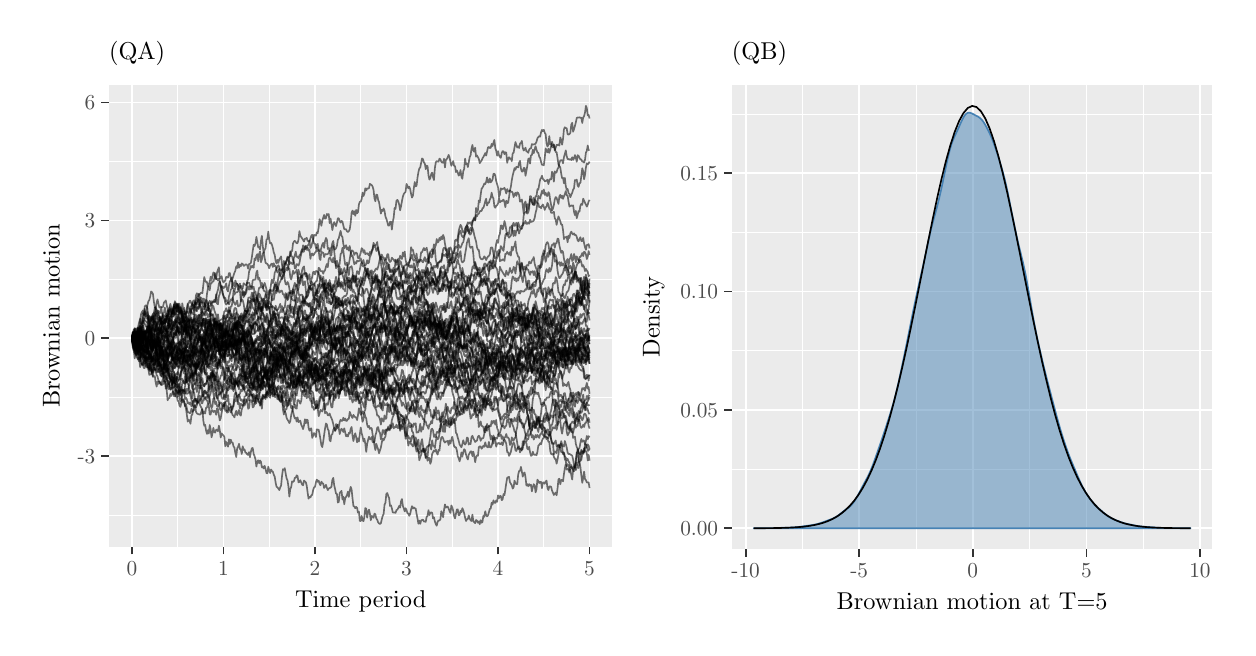
\begin{tikzpicture}[x=1pt,y=1pt]
\definecolor{fillColor}{RGB}{255,255,255}
\path[use as bounding box,fill=fillColor,fill opacity=0.00] (0,0) rectangle (433.62,216.81);
\begin{scope}
\path[clip] (  0.00,  0.00) rectangle (216.81,216.81);
\definecolor{drawColor}{RGB}{255,255,255}
\definecolor{fillColor}{RGB}{255,255,255}

\path[draw=drawColor,line width= 0.6pt,line join=round,line cap=round,fill=fillColor] (  0.00,  0.00) rectangle (216.81,216.81);
\end{scope}
\begin{scope}
\path[clip] ( 29.40, 29.26) rectangle (211.31,196.15);
\definecolor{fillColor}{gray}{0.92}

\path[fill=fillColor] ( 29.40, 29.26) rectangle (211.31,196.15);
\definecolor{drawColor}{RGB}{255,255,255}

\path[draw=drawColor,line width= 0.3pt,line join=round] ( 29.40, 40.64) --
	(211.31, 40.64);

\path[draw=drawColor,line width= 0.3pt,line join=round] ( 29.40, 83.26) --
	(211.31, 83.26);

\path[draw=drawColor,line width= 0.3pt,line join=round] ( 29.40,125.88) --
	(211.31,125.88);

\path[draw=drawColor,line width= 0.3pt,line join=round] ( 29.40,168.50) --
	(211.31,168.50);

\path[draw=drawColor,line width= 0.3pt,line join=round] ( 54.20, 29.26) --
	( 54.20,196.15);

\path[draw=drawColor,line width= 0.3pt,line join=round] ( 87.28, 29.26) --
	( 87.28,196.15);

\path[draw=drawColor,line width= 0.3pt,line join=round] (120.35, 29.26) --
	(120.35,196.15);

\path[draw=drawColor,line width= 0.3pt,line join=round] (153.43, 29.26) --
	(153.43,196.15);

\path[draw=drawColor,line width= 0.3pt,line join=round] (186.50, 29.26) --
	(186.50,196.15);

\path[draw=drawColor,line width= 0.6pt,line join=round] ( 29.40, 61.95) --
	(211.31, 61.95);

\path[draw=drawColor,line width= 0.6pt,line join=round] ( 29.40,104.57) --
	(211.31,104.57);

\path[draw=drawColor,line width= 0.6pt,line join=round] ( 29.40,147.19) --
	(211.31,147.19);

\path[draw=drawColor,line width= 0.6pt,line join=round] ( 29.40,189.80) --
	(211.31,189.80);

\path[draw=drawColor,line width= 0.6pt,line join=round] ( 37.67, 29.26) --
	( 37.67,196.15);

\path[draw=drawColor,line width= 0.6pt,line join=round] ( 70.74, 29.26) --
	( 70.74,196.15);

\path[draw=drawColor,line width= 0.6pt,line join=round] (103.82, 29.26) --
	(103.82,196.15);

\path[draw=drawColor,line width= 0.6pt,line join=round] (136.89, 29.26) --
	(136.89,196.15);

\path[draw=drawColor,line width= 0.6pt,line join=round] (169.97, 29.26) --
	(169.97,196.15);

\path[draw=drawColor,line width= 0.6pt,line join=round] (203.04, 29.26) --
	(203.04,196.15);
\definecolor{drawColor}{RGB}{0,0,0}

\path[draw=drawColor,draw opacity=0.55,line width= 0.6pt,line join=round] ( 37.67,104.57) --
	( 38.00,103.68) --
	( 38.33,103.94) --
	( 38.66,102.75) --
	( 38.99,105.02) --
	( 39.32,105.49) --
	( 39.65,104.32) --
	( 39.98,105.01) --
	( 40.31,106.06) --
	( 40.64,106.88) --
	( 40.97,106.45) --
	( 41.30,108.59) --
	( 41.64,109.15) --
	( 41.97,108.26) --
	( 42.30,105.12) --
	( 42.63,106.72) --
	( 42.96,106.65) --
	( 43.29,106.63) --
	( 43.62,107.97) --
	( 43.95,109.14) --
	( 44.28,109.98) --
	( 44.61,111.29) --
	( 44.94,112.40) --
	( 45.27,112.50) --
	( 45.60,109.68) --
	( 45.94,110.56) --
	( 46.27,110.48) --
	( 46.60,110.26) --
	( 46.93,108.17) --
	( 47.26,107.49) --
	( 47.59,108.08) --
	( 47.92,110.01) --
	( 48.25,109.87) --
	( 48.58,110.42) --
	( 48.91,110.34) --
	( 49.24,108.38) --
	( 49.57,107.79) --
	( 49.90,107.23) --
	( 50.24,107.15) --
	( 50.57,108.71) --
	( 50.90,109.80) --
	( 51.23,109.56) --
	( 51.56,109.20) --
	( 51.89,110.19) --
	( 52.22,110.98) --
	( 52.55,110.01) --
	( 52.88,109.00) --
	( 53.21,109.52) --
	( 53.54,110.61) --
	( 53.87,110.45) --
	( 54.20,111.70) --
	( 54.53,112.27) --
	( 54.87,111.40) --
	( 55.20,111.88) --
	( 55.53,110.28) --
	( 55.86,112.31) --
	( 56.19,115.13) --
	( 56.52,114.61) --
	( 56.85,113.12) --
	( 57.18,113.93) --
	( 57.51,113.74) --
	( 57.84,117.15) --
	( 58.17,117.10) --
	( 58.50,118.08) --
	( 58.83,118.12) --
	( 59.17,117.06) --
	( 59.50,117.33) --
	( 59.83,114.76) --
	( 60.16,116.85) --
	( 60.49,117.06) --
	( 60.82,120.15) --
	( 61.15,120.83) --
	( 61.48,119.82) --
	( 61.81,120.69) --
	( 62.14,119.36) --
	( 62.47,117.58) --
	( 62.80,117.99) --
	( 63.13,117.36) --
	( 63.47,117.36) --
	( 63.80,117.47) --
	( 64.13,116.63) --
	( 64.46,115.82) --
	( 64.79,115.63) --
	( 65.12,117.31) --
	( 65.45,115.14) --
	( 65.78,115.98) --
	( 66.11,116.46) --
	( 66.44,117.97) --
	( 66.77,117.54) --
	( 67.10,118.06) --
	( 67.43,118.44) --
	( 67.76,117.67) --
	( 68.10,119.39) --
	( 68.43,121.03) --
	( 68.76,122.03) --
	( 69.09,124.28) --
	( 69.42,125.08) --
	( 69.75,123.26) --
	( 70.08,122.45) --
	( 70.41,120.71) --
	( 70.74,120.04) --
	( 71.07,119.16) --
	( 71.40,119.22) --
	( 71.73,117.92) --
	( 72.06,118.15) --
	( 72.40,117.22) --
	( 72.73,119.73) --
	( 73.06,120.74) --
	( 73.39,122.04) --
	( 73.72,122.58) --
	( 74.05,124.97) --
	( 74.38,124.07) --
	( 74.71,123.41) --
	( 75.04,125.45) --
	( 75.37,124.52) --
	( 75.70,124.23) --
	( 76.03,123.67) --
	( 76.36,123.22) --
	( 76.70,122.82) --
	( 77.03,123.52) --
	( 77.36,123.27) --
	( 77.69,122.55) --
	( 78.02,124.46) --
	( 78.35,124.15) --
	( 78.68,123.90) --
	( 79.01,123.76) --
	( 79.34,124.77) --
	( 79.67,124.67) --
	( 80.00,124.61) --
	( 80.33,123.64) --
	( 80.66,123.18) --
	( 80.99,123.27) --
	( 81.33,122.43) --
	( 81.66,123.19) --
	( 81.99,121.03) --
	( 82.32,121.47) --
	( 82.65,119.28) --
	( 82.98,118.86) --
	( 83.31,118.10) --
	( 83.64,117.18) --
	( 83.97,117.10) --
	( 84.30,114.38) --
	( 84.63,116.05) --
	( 84.96,113.68) --
	( 85.29,113.03) --
	( 85.63,111.44) --
	( 85.96,110.37) --
	( 86.29,113.34) --
	( 86.62,113.36) --
	( 86.95,111.54) --
	( 87.28,109.21) --
	( 87.61,109.85) --
	( 87.94,109.82) --
	( 88.27,109.37) --
	( 88.60,108.05) --
	( 88.93,105.93) --
	( 89.26,104.41) --
	( 89.59,105.83) --
	( 89.93,104.94) --
	( 90.26,102.98) --
	( 90.59,105.63) --
	( 90.92,106.24) --
	( 91.25,105.90) --
	( 91.58,107.40) --
	( 91.91,108.66) --
	( 92.24,107.78) --
	( 92.57,110.92) --
	( 92.90,110.55) --
	( 93.23,108.53) --
	( 93.56,108.32) --
	( 93.89,108.62) --
	( 94.22,111.90) --
	( 94.56,112.05) --
	( 94.89,112.70) --
	( 95.22,112.59) --
	( 95.55,112.11) --
	( 95.88,112.06) --
	( 96.21,113.18) --
	( 96.54,116.13) --
	( 96.87,117.59) --
	( 97.20,119.31) --
	( 97.53,117.56) --
	( 97.86,118.95) --
	( 98.19,119.27) --
	( 98.52,117.18) --
	( 98.86,117.92) --
	( 99.19,117.70) --
	( 99.52,119.78) --
	( 99.85,118.69) --
	(100.18,118.08) --
	(100.51,116.76) --
	(100.84,116.51) --
	(101.17,117.08) --
	(101.50,116.04) --
	(101.83,117.22) --
	(102.16,115.51) --
	(102.49,114.02) --
	(102.82,116.06) --
	(103.15,114.62) --
	(103.49,115.21) --
	(103.82,114.67) --
	(104.15,115.25) --
	(104.48,117.65) --
	(104.81,119.90) --
	(105.14,119.43) --
	(105.47,116.18) --
	(105.80,119.73) --
	(106.13,120.68) --
	(106.46,121.45) --
	(106.79,121.43) --
	(107.12,122.15) --
	(107.45,121.92) --
	(107.79,122.52) --
	(108.12,121.95) --
	(108.45,120.00) --
	(108.78,121.41) --
	(109.11,123.57) --
	(109.44,123.13) --
	(109.77,121.35) --
	(110.10,122.26) --
	(110.43,122.20) --
	(110.76,119.73) --
	(111.09,119.74) --
	(111.42,118.84) --
	(111.75,118.36) --
	(112.09,116.71) --
	(112.42,119.27) --
	(112.75,118.80) --
	(113.08,116.52) --
	(113.41,116.80) --
	(113.74,117.18) --
	(114.07,115.78) --
	(114.40,111.67) --
	(114.73,110.76) --
	(115.06,111.57) --
	(115.39,111.49) --
	(115.72,111.35) --
	(116.05,112.15) --
	(116.38,110.46) --
	(116.72,112.02) --
	(117.05,112.01) --
	(117.38,113.02) --
	(117.71,114.49) --
	(118.04,114.80) --
	(118.37,113.55) --
	(118.70,115.21) --
	(119.03,112.36) --
	(119.36,111.59) --
	(119.69,111.23) --
	(120.02,110.99) --
	(120.35,112.44) --
	(120.68,112.63) --
	(121.02,113.21) --
	(121.35,113.11) --
	(121.68,112.76) --
	(122.01,113.75) --
	(122.34,115.38) --
	(122.67,111.97) --
	(123.00,112.78) --
	(123.33,113.31) --
	(123.66,112.71) --
	(123.99,114.06) --
	(124.32,113.51) --
	(124.65,113.10) --
	(124.98,114.32) --
	(125.32,116.76) --
	(125.65,117.15) --
	(125.98,116.55) --
	(126.31,114.86) --
	(126.64,114.39) --
	(126.97,113.05) --
	(127.30,112.68) --
	(127.63,113.24) --
	(127.96,112.03) --
	(128.29,115.80) --
	(128.62,116.02) --
	(128.95,117.62) --
	(129.28,114.37) --
	(129.61,115.42) --
	(129.95,113.56) --
	(130.28,114.86) --
	(130.61,115.43) --
	(130.94,114.85) --
	(131.27,116.73) --
	(131.60,115.73) --
	(131.93,114.91) --
	(132.26,113.49) --
	(132.59,112.54) --
	(132.92,113.88) --
	(133.25,114.50) --
	(133.58,115.92) --
	(133.91,115.37) --
	(134.25,115.90) --
	(134.58,116.25) --
	(134.91,114.23) --
	(135.24,116.75) --
	(135.57,116.94) --
	(135.90,118.03) --
	(136.23,119.39) --
	(136.56,119.32) --
	(136.89,118.88) --
	(137.22,120.15) --
	(137.55,118.66) --
	(137.88,121.46) --
	(138.21,120.92) --
	(138.55,123.27) --
	(138.88,125.42) --
	(139.21,125.53) --
	(139.54,126.34) --
	(139.87,124.88) --
	(140.20,125.34) --
	(140.53,126.83) --
	(140.86,126.97) --
	(141.19,126.32) --
	(141.52,125.39) --
	(141.85,125.34) --
	(142.18,126.86) --
	(142.51,126.17) --
	(142.84,126.00) --
	(143.18,124.16) --
	(143.51,124.86) --
	(143.84,126.72) --
	(144.17,128.85) --
	(144.50,130.00) --
	(144.83,127.35) --
	(145.16,128.03) --
	(145.49,128.68) --
	(145.82,128.18) --
	(146.15,128.42) --
	(146.48,127.19) --
	(146.81,128.16) --
	(147.14,127.69) --
	(147.48,125.46) --
	(147.81,124.94) --
	(148.14,126.88) --
	(148.47,126.41) --
	(148.80,127.45) --
	(149.13,128.79) --
	(149.46,128.80) --
	(149.79,128.30) --
	(150.12,127.54) --
	(150.45,128.60) --
	(150.78,127.08) --
	(151.11,127.43) --
	(151.44,127.02) --
	(151.78,123.81) --
	(152.11,121.80) --
	(152.44,123.11) --
	(152.77,122.83) --
	(153.10,123.98) --
	(153.43,126.66) --
	(153.76,128.75) --
	(154.09,129.71) --
	(154.42,130.25) --
	(154.75,129.98) --
	(155.08,132.22) --
	(155.41,133.07) --
	(155.74,131.40) --
	(156.07,131.18) --
	(156.41,128.45) --
	(156.74,128.18) --
	(157.07,124.49) --
	(157.40,126.36) --
	(157.73,125.46) --
	(158.06,124.85) --
	(158.39,124.61) --
	(158.72,125.47) --
	(159.05,126.44) --
	(159.38,127.25) --
	(159.71,126.43) --
	(160.04,124.50) --
	(160.37,123.94) --
	(160.71,124.34) --
	(161.04,123.17) --
	(161.37,123.07) --
	(161.70,121.41) --
	(162.03,121.40) --
	(162.36,121.58) --
	(162.69,121.38) --
	(163.02,121.14) --
	(163.35,123.65) --
	(163.68,124.73) --
	(164.01,126.31) --
	(164.34,125.00) --
	(164.67,125.23) --
	(165.01,126.87) --
	(165.34,126.79) --
	(165.67,123.77) --
	(166.00,124.26) --
	(166.33,121.55) --
	(166.66,120.40) --
	(166.99,122.28) --
	(167.32,123.15) --
	(167.65,124.71) --
	(167.98,125.14) --
	(168.31,124.98) --
	(168.64,123.67) --
	(168.97,125.93) --
	(169.30,126.00) --
	(169.64,124.98) --
	(169.97,126.21) --
	(170.30,127.74) --
	(170.63,130.43) --
	(170.96,129.57) --
	(171.29,129.02) --
	(171.62,128.43) --
	(171.95,127.89) --
	(172.28,127.37) --
	(172.61,126.95) --
	(172.94,129.00) --
	(173.27,128.01) --
	(173.60,127.46) --
	(173.94,128.39) --
	(174.27,129.98) --
	(174.60,128.89) --
	(174.93,128.17) --
	(175.26,128.91) --
	(175.59,130.35) --
	(175.92,130.00) --
	(176.25,127.97) --
	(176.58,130.39) --
	(176.91,132.43) --
	(177.24,131.42) --
	(177.57,131.33) --
	(177.90,128.83) --
	(178.24,129.64) --
	(178.57,131.93) --
	(178.90,129.61) --
	(179.23,128.50) --
	(179.56,127.59) --
	(179.89,126.62) --
	(180.22,123.73) --
	(180.55,124.44) --
	(180.88,122.27) --
	(181.21,122.23) --
	(181.54,123.07) --
	(181.87,122.79) --
	(182.20,124.06) --
	(182.53,124.02) --
	(182.87,123.10) --
	(183.20,124.02) --
	(183.53,123.41) --
	(183.86,125.92) --
	(184.19,125.90) --
	(184.52,127.11) --
	(184.85,127.40) --
	(185.18,123.13) --
	(185.51,121.19) --
	(185.84,120.58) --
	(186.17,120.92) --
	(186.50,117.59) --
	(186.83,118.96) --
	(187.17,118.10) --
	(187.50,117.03) --
	(187.83,114.82) --
	(188.16,112.75) --
	(188.49,112.83) --
	(188.82,113.56) --
	(189.15,110.58) --
	(189.48,109.15) --
	(189.81,109.91) --
	(190.14,109.27) --
	(190.47,112.35) --
	(190.80,114.11) --
	(191.13,114.96) --
	(191.47,114.97) --
	(191.80,115.36) --
	(192.13,114.36) --
	(192.46,115.25) --
	(192.79,117.36) --
	(193.12,118.90) --
	(193.45,117.74) --
	(193.78,115.44) --
	(194.11,115.29) --
	(194.44,115.91) --
	(194.77,117.83) --
	(195.10,115.96) --
	(195.43,116.48) --
	(195.76,116.81) --
	(196.10,118.50) --
	(196.43,118.46) --
	(196.76,117.96) --
	(197.09,116.33) --
	(197.42,115.59) --
	(197.75,115.08) --
	(198.08,118.42) --
	(198.41,121.89) --
	(198.74,121.65) --
	(199.07,120.17) --
	(199.40,117.37) --
	(199.73,118.10) --
	(200.06,116.55) --
	(200.40,119.80) --
	(200.73,118.54) --
	(201.06,118.70) --
	(201.39,124.11) --
	(201.72,122.53) --
	(202.05,122.97) --
	(202.38,121.40) --
	(202.71,121.89) --
	(203.04,120.65);

\path[draw=drawColor,draw opacity=0.55,line width= 0.6pt,line join=round] ( 37.67,104.57) --
	( 38.00,106.78) --
	( 38.33,105.75) --
	( 38.66,103.61) --
	( 38.99,102.80) --
	( 39.32, 99.81) --
	( 39.65,100.57) --
	( 39.98,102.87) --
	( 40.31,104.55) --
	( 40.64,107.21) --
	( 40.97,106.57) --
	( 41.30,107.52) --
	( 41.64,105.69) --
	( 41.97,105.13) --
	( 42.30,104.96) --
	( 42.63,103.60) --
	( 42.96,104.20) --
	( 43.29,104.05) --
	( 43.62,103.62) --
	( 43.95,104.06) --
	( 44.28,104.42) --
	( 44.61,104.67) --
	( 44.94,103.15) --
	( 45.27,103.29) --
	( 45.60,101.57) --
	( 45.94,102.19) --
	( 46.27, 99.04) --
	( 46.60,102.93) --
	( 46.93,103.31) --
	( 47.26,101.15) --
	( 47.59,101.14) --
	( 47.92, 97.67) --
	( 48.25, 98.10) --
	( 48.58, 94.88) --
	( 48.91, 94.28) --
	( 49.24, 94.11) --
	( 49.57, 93.57) --
	( 49.90, 92.38) --
	( 50.24, 93.35) --
	( 50.57, 94.51) --
	( 50.90, 92.21) --
	( 51.23, 92.08) --
	( 51.56, 90.44) --
	( 51.89, 89.40) --
	( 52.22, 90.63) --
	( 52.55, 88.31) --
	( 52.88, 89.20) --
	( 53.21, 88.30) --
	( 53.54, 88.41) --
	( 53.87, 90.38) --
	( 54.20, 90.56) --
	( 54.53, 89.46) --
	( 54.87, 90.74) --
	( 55.20, 89.82) --
	( 55.53, 91.80) --
	( 55.86, 93.46) --
	( 56.19, 94.07) --
	( 56.52, 94.49) --
	( 56.85, 94.09) --
	( 57.18, 91.52) --
	( 57.51, 93.36) --
	( 57.84, 93.47) --
	( 58.17, 92.38) --
	( 58.50, 91.68) --
	( 58.83, 90.28) --
	( 59.17, 90.32) --
	( 59.50, 89.18) --
	( 59.83, 85.25) --
	( 60.16, 85.01) --
	( 60.49, 82.44) --
	( 60.82, 82.12) --
	( 61.15, 80.84) --
	( 61.48, 81.70) --
	( 61.81, 81.71) --
	( 62.14, 83.74) --
	( 62.47, 83.57) --
	( 62.80, 81.08) --
	( 63.13, 81.08) --
	( 63.47, 82.55) --
	( 63.80, 82.33) --
	( 64.13, 83.09) --
	( 64.46, 83.02) --
	( 64.79, 83.47) --
	( 65.12, 84.15) --
	( 65.45, 83.72) --
	( 65.78, 82.49) --
	( 66.11, 80.26) --
	( 66.44, 79.31) --
	( 66.77, 80.11) --
	( 67.10, 82.78) --
	( 67.43, 82.97) --
	( 67.76, 80.80) --
	( 68.10, 81.68) --
	( 68.43, 80.04) --
	( 68.76, 79.82) --
	( 69.09, 80.39) --
	( 69.42, 81.13) --
	( 69.75, 81.42) --
	( 70.08, 80.96) --
	( 70.41, 79.85) --
	( 70.74, 81.24) --
	( 71.07, 80.35) --
	( 71.40, 78.33) --
	( 71.73, 78.50) --
	( 72.06, 77.68) --
	( 72.40, 77.83) --
	( 72.73, 79.42) --
	( 73.06, 79.54) --
	( 73.39, 79.75) --
	( 73.72, 78.83) --
	( 74.05, 80.00) --
	( 74.38, 79.95) --
	( 74.71, 82.21) --
	( 75.04, 81.79) --
	( 75.37, 83.67) --
	( 75.70, 81.96) --
	( 76.03, 80.76) --
	( 76.36, 81.22) --
	( 76.70, 79.15) --
	( 77.03, 80.89) --
	( 77.36, 80.65) --
	( 77.69, 80.18) --
	( 78.02, 80.83) --
	( 78.35, 80.23) --
	( 78.68, 81.03) --
	( 79.01, 81.65) --
	( 79.34, 82.50) --
	( 79.67, 83.47) --
	( 80.00, 82.08) --
	( 80.33, 84.23) --
	( 80.66, 84.35) --
	( 80.99, 83.91) --
	( 81.33, 84.12) --
	( 81.66, 81.90) --
	( 81.99, 81.55) --
	( 82.32, 80.81) --
	( 82.65, 84.34) --
	( 82.98, 86.79) --
	( 83.31, 87.35) --
	( 83.64, 86.78) --
	( 83.97, 87.86) --
	( 84.30, 87.67) --
	( 84.63, 88.16) --
	( 84.96, 86.40) --
	( 85.29, 89.92) --
	( 85.63, 92.01) --
	( 85.96, 92.29) --
	( 86.29, 92.23) --
	( 86.62, 90.99) --
	( 86.95, 90.96) --
	( 87.28, 90.76) --
	( 87.61, 90.82) --
	( 87.94, 91.50) --
	( 88.27, 92.25) --
	( 88.60, 95.07) --
	( 88.93, 95.59) --
	( 89.26, 95.98) --
	( 89.59, 95.39) --
	( 89.93, 95.66) --
	( 90.26, 94.27) --
	( 90.59, 93.43) --
	( 90.92, 94.74) --
	( 91.25, 94.03) --
	( 91.58, 94.11) --
	( 91.91, 93.60) --
	( 92.24, 93.77) --
	( 92.57, 92.83) --
	( 92.90, 94.17) --
	( 93.23, 94.52) --
	( 93.56, 94.77) --
	( 93.89, 93.30) --
	( 94.22, 94.05) --
	( 94.56, 93.61) --
	( 94.89, 96.84) --
	( 95.22, 99.70) --
	( 95.55,100.06) --
	( 95.88, 98.55) --
	( 96.21, 99.65) --
	( 96.54,100.46) --
	( 96.87, 99.59) --
	( 97.20,101.74) --
	( 97.53,101.11) --
	( 97.86, 99.75) --
	( 98.19,101.09) --
	( 98.52,101.45) --
	( 98.86, 99.57) --
	( 99.19, 98.67) --
	( 99.52, 97.71) --
	( 99.85, 96.38) --
	(100.18, 97.55) --
	(100.51, 97.48) --
	(100.84,100.59) --
	(101.17,101.47) --
	(101.50,103.35) --
	(101.83,104.84) --
	(102.16,104.68) --
	(102.49,105.01) --
	(102.82,107.08) --
	(103.15,107.33) --
	(103.49,106.54) --
	(103.82,107.38) --
	(104.15,107.31) --
	(104.48,108.12) --
	(104.81,109.11) --
	(105.14,110.87) --
	(105.47,110.77) --
	(105.80,110.44) --
	(106.13,112.66) --
	(106.46,113.21) --
	(106.79,112.34) --
	(107.12,112.13) --
	(107.45,111.63) --
	(107.79,110.87) --
	(108.12,108.56) --
	(108.45,109.98) --
	(108.78,107.62) --
	(109.11,108.62) --
	(109.44,106.18) --
	(109.77,103.41) --
	(110.10,102.10) --
	(110.43,102.69) --
	(110.76,104.34) --
	(111.09,105.70) --
	(111.42,103.56) --
	(111.75,104.44) --
	(112.09,104.56) --
	(112.42,104.98) --
	(112.75,103.29) --
	(113.08,101.73) --
	(113.41,103.62) --
	(113.74,103.85) --
	(114.07,104.98) --
	(114.40,105.01) --
	(114.73,104.66) --
	(115.06,101.23) --
	(115.39,103.03) --
	(115.72,105.77) --
	(116.05,108.09) --
	(116.38,108.53) --
	(116.72,110.68) --
	(117.05,112.05) --
	(117.38,112.63) --
	(117.71,114.07) --
	(118.04,114.01) --
	(118.37,111.30) --
	(118.70,112.62) --
	(119.03,113.94) --
	(119.36,115.50) --
	(119.69,113.17) --
	(120.02,112.11) --
	(120.35,111.90) --
	(120.68,114.54) --
	(121.02,113.69) --
	(121.35,112.49) --
	(121.68,115.85) --
	(122.01,115.87) --
	(122.34,115.94) --
	(122.67,114.83) --
	(123.00,116.16) --
	(123.33,118.19) --
	(123.66,116.52) --
	(123.99,116.74) --
	(124.32,117.88) --
	(124.65,119.50) --
	(124.98,118.78) --
	(125.32,115.12) --
	(125.65,114.85) --
	(125.98,115.33) --
	(126.31,116.47) --
	(126.64,114.37) --
	(126.97,113.60) --
	(127.30,113.06) --
	(127.63,112.34) --
	(127.96,113.90) --
	(128.29,112.03) --
	(128.62,111.10) --
	(128.95,109.42) --
	(129.28,107.32) --
	(129.61,108.85) --
	(129.95,108.01) --
	(130.28,108.50) --
	(130.61,107.04) --
	(130.94,108.82) --
	(131.27,105.86) --
	(131.60,106.20) --
	(131.93,105.47) --
	(132.26,106.43) --
	(132.59,104.87) --
	(132.92,106.44) --
	(133.25,105.23) --
	(133.58,103.64) --
	(133.91,104.78) --
	(134.25,106.32) --
	(134.58,106.87) --
	(134.91,106.22) --
	(135.24,105.93) --
	(135.57,105.68) --
	(135.90,103.59) --
	(136.23,103.74) --
	(136.56,103.94) --
	(136.89,102.98) --
	(137.22,101.36) --
	(137.55,103.03) --
	(137.88,102.36) --
	(138.21,104.69) --
	(138.55,104.22) --
	(138.88,104.44) --
	(139.21,105.51) --
	(139.54,106.83) --
	(139.87,108.53) --
	(140.20,108.87) --
	(140.53,109.80) --
	(140.86,111.85) --
	(141.19,112.35) --
	(141.52,114.51) --
	(141.85,114.94) --
	(142.18,113.62) --
	(142.51,114.41) --
	(142.84,112.28) --
	(143.18,113.01) --
	(143.51,111.29) --
	(143.84,110.83) --
	(144.17,111.79) --
	(144.50,110.73) --
	(144.83,108.66) --
	(145.16,108.52) --
	(145.49,107.67) --
	(145.82,109.29) --
	(146.15,107.73) --
	(146.48,105.74) --
	(146.81,104.66) --
	(147.14,106.70) --
	(147.48,107.93) --
	(147.81,106.88) --
	(148.14,104.69) --
	(148.47,105.23) --
	(148.80,103.17) --
	(149.13,102.96) --
	(149.46,101.99) --
	(149.79,101.43) --
	(150.12,101.99) --
	(150.45,102.85) --
	(150.78,103.26) --
	(151.11,100.95) --
	(151.44,101.87) --
	(151.78,101.33) --
	(152.11,102.91) --
	(152.44,103.46) --
	(152.77,102.83) --
	(153.10,105.75) --
	(153.43,106.39) --
	(153.76,104.91) --
	(154.09,104.83) --
	(154.42,103.40) --
	(154.75,101.46) --
	(155.08,101.78) --
	(155.41,102.13) --
	(155.74,103.28) --
	(156.07,105.42) --
	(156.41,106.03) --
	(156.74,106.04) --
	(157.07,106.16) --
	(157.40,107.39) --
	(157.73,106.01) --
	(158.06,104.74) --
	(158.39,103.29) --
	(158.72,104.60) --
	(159.05,105.57) --
	(159.38,103.26) --
	(159.71,104.29) --
	(160.04,102.64) --
	(160.37,102.88) --
	(160.71,104.37) --
	(161.04,103.26) --
	(161.37,104.06) --
	(161.70,103.61) --
	(162.03,105.33) --
	(162.36,106.26) --
	(162.69,107.09) --
	(163.02,104.60) --
	(163.35,103.96) --
	(163.68,101.34) --
	(164.01,101.03) --
	(164.34,100.70) --
	(164.67,100.18) --
	(165.01, 99.69) --
	(165.34, 99.24) --
	(165.67, 97.42) --
	(166.00, 96.40) --
	(166.33, 95.58) --
	(166.66, 96.01) --
	(166.99, 98.06) --
	(167.32, 97.19) --
	(167.65, 94.28) --
	(167.98, 93.79) --
	(168.31, 92.38) --
	(168.64, 93.10) --
	(168.97, 92.99) --
	(169.30, 93.71) --
	(169.64, 95.64) --
	(169.97, 95.30) --
	(170.30, 92.29) --
	(170.63, 91.35) --
	(170.96, 91.80) --
	(171.29, 91.66) --
	(171.62, 91.61) --
	(171.95, 90.26) --
	(172.28, 89.49) --
	(172.61, 90.31) --
	(172.94, 93.68) --
	(173.27, 95.08) --
	(173.60, 98.10) --
	(173.94, 97.28) --
	(174.27, 95.97) --
	(174.60, 95.80) --
	(174.93, 97.09) --
	(175.26, 98.90) --
	(175.59, 96.09) --
	(175.92, 95.23) --
	(176.25, 92.99) --
	(176.58, 94.59) --
	(176.91, 97.08) --
	(177.24, 98.76) --
	(177.57, 98.88) --
	(177.90, 96.64) --
	(178.24, 95.98) --
	(178.57, 93.99) --
	(178.90, 96.07) --
	(179.23, 94.30) --
	(179.56, 95.23) --
	(179.89, 94.76) --
	(180.22, 92.74) --
	(180.55, 92.41) --
	(180.88, 95.34) --
	(181.21, 97.75) --
	(181.54, 95.28) --
	(181.87, 93.48) --
	(182.20, 92.07) --
	(182.53, 93.60) --
	(182.87, 92.97) --
	(183.20, 92.78) --
	(183.53, 93.83) --
	(183.86, 92.73) --
	(184.19, 93.27) --
	(184.52, 93.77) --
	(184.85, 93.63) --
	(185.18, 95.64) --
	(185.51, 94.91) --
	(185.84, 94.88) --
	(186.17, 93.57) --
	(186.50, 92.99) --
	(186.83, 90.84) --
	(187.17, 91.20) --
	(187.50, 93.43) --
	(187.83, 91.52) --
	(188.16, 90.19) --
	(188.49, 90.13) --
	(188.82, 87.54) --
	(189.15, 86.65) --
	(189.48, 86.11) --
	(189.81, 84.55) --
	(190.14, 84.23) --
	(190.47, 85.42) --
	(190.80, 85.75) --
	(191.13, 85.33) --
	(191.47, 84.87) --
	(191.80, 82.42) --
	(192.13, 81.69) --
	(192.46, 81.90) --
	(192.79, 82.42) --
	(193.12, 81.51) --
	(193.45, 82.97) --
	(193.78, 84.67) --
	(194.11, 84.77) --
	(194.44, 82.97) --
	(194.77, 81.50) --
	(195.10, 81.96) --
	(195.43, 82.59) --
	(195.76, 83.08) --
	(196.10, 84.86) --
	(196.43, 84.83) --
	(196.76, 83.31) --
	(197.09, 85.03) --
	(197.42, 83.78) --
	(197.75, 83.95) --
	(198.08, 84.72) --
	(198.41, 84.53) --
	(198.74, 85.11) --
	(199.07, 85.06) --
	(199.40, 83.46) --
	(199.73, 82.53) --
	(200.06, 81.56) --
	(200.40, 82.59) --
	(200.73, 84.23) --
	(201.06, 81.67) --
	(201.39, 79.68) --
	(201.72, 79.91) --
	(202.05, 81.31) --
	(202.38, 80.32) --
	(202.71, 80.32) --
	(203.04, 80.56);

\path[draw=drawColor,draw opacity=0.55,line width= 0.6pt,line join=round] ( 37.67,104.57) --
	( 38.00,102.41) --
	( 38.33,103.31) --
	( 38.66,100.92) --
	( 38.99,102.60) --
	( 39.32,104.19) --
	( 39.65,102.43) --
	( 39.98,100.68) --
	( 40.31,101.53) --
	( 40.64,101.96) --
	( 40.97,101.80) --
	( 41.30,100.65) --
	( 41.64,100.81) --
	( 41.97,100.56) --
	( 42.30,100.64) --
	( 42.63,102.48) --
	( 42.96,101.87) --
	( 43.29,100.72) --
	( 43.62, 99.97) --
	( 43.95, 99.57) --
	( 44.28, 98.65) --
	( 44.61, 99.14) --
	( 44.94,101.20) --
	( 45.27,103.12) --
	( 45.60,103.79) --
	( 45.94,103.44) --
	( 46.27,101.39) --
	( 46.60, 99.99) --
	( 46.93, 98.30) --
	( 47.26, 98.21) --
	( 47.59,100.98) --
	( 47.92, 98.99) --
	( 48.25, 97.31) --
	( 48.58, 96.97) --
	( 48.91, 96.44) --
	( 49.24, 95.64) --
	( 49.57, 94.22) --
	( 49.90, 95.47) --
	( 50.24, 95.75) --
	( 50.57, 93.58) --
	( 50.90, 93.16) --
	( 51.23, 93.32) --
	( 51.56, 94.47) --
	( 51.89, 92.41) --
	( 52.22, 94.83) --
	( 52.55, 92.55) --
	( 52.88, 92.50) --
	( 53.21, 91.28) --
	( 53.54, 90.13) --
	( 53.87, 89.10) --
	( 54.20, 88.26) --
	( 54.53, 87.37) --
	( 54.87, 86.24) --
	( 55.20, 84.44) --
	( 55.53, 84.24) --
	( 55.86, 81.35) --
	( 56.19, 82.56) --
	( 56.52, 81.86) --
	( 56.85, 80.31) --
	( 57.18, 79.28) --
	( 57.51, 76.97) --
	( 57.84, 74.46) --
	( 58.17, 75.19) --
	( 58.50, 74.80) --
	( 58.83, 73.68) --
	( 59.17, 76.61) --
	( 59.50, 77.09) --
	( 59.83, 78.61) --
	( 60.16, 80.39) --
	( 60.49, 79.99) --
	( 60.82, 79.52) --
	( 61.15, 80.40) --
	( 61.48, 83.12) --
	( 61.81, 84.51) --
	( 62.14, 86.40) --
	( 62.47, 86.79) --
	( 62.80, 89.58) --
	( 63.13, 87.69) --
	( 63.47, 87.75) --
	( 63.80, 87.16) --
	( 64.13, 88.28) --
	( 64.46, 88.24) --
	( 64.79, 88.80) --
	( 65.12, 90.81) --
	( 65.45, 90.86) --
	( 65.78, 89.39) --
	( 66.11, 90.72) --
	( 66.44, 89.39) --
	( 66.77, 87.65) --
	( 67.10, 86.84) --
	( 67.43, 85.48) --
	( 67.76, 86.66) --
	( 68.10, 86.04) --
	( 68.43, 85.58) --
	( 68.76, 86.50) --
	( 69.09, 84.12) --
	( 69.42, 84.70) --
	( 69.75, 85.02) --
	( 70.08, 85.04) --
	( 70.41, 86.65) --
	( 70.74, 88.86) --
	( 71.07, 90.11) --
	( 71.40, 92.07) --
	( 71.73, 93.98) --
	( 72.06, 92.90) --
	( 72.40, 92.48) --
	( 72.73, 93.90) --
	( 73.06, 94.71) --
	( 73.39, 94.27) --
	( 73.72, 95.29) --
	( 74.05, 94.45) --
	( 74.38, 93.21) --
	( 74.71, 92.69) --
	( 75.04, 93.41) --
	( 75.37, 93.23) --
	( 75.70, 94.20) --
	( 76.03, 94.59) --
	( 76.36, 94.18) --
	( 76.70, 93.30) --
	( 77.03, 93.62) --
	( 77.36, 93.00) --
	( 77.69, 90.62) --
	( 78.02, 91.57) --
	( 78.35, 91.45) --
	( 78.68, 90.68) --
	( 79.01, 90.70) --
	( 79.34, 90.04) --
	( 79.67, 91.64) --
	( 80.00, 90.97) --
	( 80.33, 91.59) --
	( 80.66, 92.19) --
	( 80.99, 92.17) --
	( 81.33, 94.04) --
	( 81.66, 92.65) --
	( 81.99, 94.37) --
	( 82.32, 94.19) --
	( 82.65, 94.78) --
	( 82.98, 92.04) --
	( 83.31, 89.40) --
	( 83.64, 91.76) --
	( 83.97, 92.15) --
	( 84.30, 92.86) --
	( 84.63, 93.77) --
	( 84.96, 94.21) --
	( 85.29, 92.19) --
	( 85.63, 91.82) --
	( 85.96, 92.27) --
	( 86.29, 94.24) --
	( 86.62, 92.24) --
	( 86.95, 88.76) --
	( 87.28, 87.05) --
	( 87.61, 85.15) --
	( 87.94, 86.64) --
	( 88.27, 85.79) --
	( 88.60, 83.50) --
	( 88.93, 83.78) --
	( 89.26, 84.45) --
	( 89.59, 84.41) --
	( 89.93, 85.82) --
	( 90.26, 87.02) --
	( 90.59, 86.02) --
	( 90.92, 86.30) --
	( 91.25, 85.04) --
	( 91.58, 87.33) --
	( 91.91, 86.35) --
	( 92.24, 87.65) --
	( 92.57, 87.44) --
	( 92.90, 86.36) --
	( 93.23, 86.30) --
	( 93.56, 87.08) --
	( 93.89, 86.78) --
	( 94.22, 87.07) --
	( 94.56, 86.73) --
	( 94.89, 87.50) --
	( 95.22, 90.74) --
	( 95.55, 91.84) --
	( 95.88, 91.53) --
	( 96.21, 90.74) --
	( 96.54, 92.57) --
	( 96.87, 93.42) --
	( 97.20, 93.87) --
	( 97.53, 93.08) --
	( 97.86, 95.73) --
	( 98.19, 96.21) --
	( 98.52, 95.45) --
	( 98.86, 93.92) --
	( 99.19, 95.37) --
	( 99.52, 96.15) --
	( 99.85, 98.73) --
	(100.18,100.33) --
	(100.51, 98.33) --
	(100.84, 99.43) --
	(101.17, 98.14) --
	(101.50, 98.36) --
	(101.83, 97.68) --
	(102.16, 97.56) --
	(102.49, 97.96) --
	(102.82, 99.21) --
	(103.15, 99.89) --
	(103.49, 99.41) --
	(103.82, 98.57) --
	(104.15, 99.22) --
	(104.48,101.56) --
	(104.81,103.42) --
	(105.14,103.67) --
	(105.47,102.68) --
	(105.80,103.92) --
	(106.13,102.80) --
	(106.46,103.58) --
	(106.79,104.05) --
	(107.12,102.89) --
	(107.45,101.34) --
	(107.79,100.72) --
	(108.12,100.46) --
	(108.45,102.50) --
	(108.78,102.66) --
	(109.11,102.35) --
	(109.44,101.13) --
	(109.77,102.69) --
	(110.10,102.94) --
	(110.43,102.02) --
	(110.76,102.45) --
	(111.09,101.14) --
	(111.42,100.51) --
	(111.75, 99.98) --
	(112.09, 98.82) --
	(112.42, 98.00) --
	(112.75, 99.44) --
	(113.08, 99.53) --
	(113.41, 96.79) --
	(113.74, 95.77) --
	(114.07, 96.27) --
	(114.40, 96.89) --
	(114.73, 94.76) --
	(115.06, 94.83) --
	(115.39, 93.88) --
	(115.72, 93.38) --
	(116.05, 92.16) --
	(116.38, 93.08) --
	(116.72, 92.07) --
	(117.05, 91.51) --
	(117.38, 91.71) --
	(117.71, 94.74) --
	(118.04, 94.62) --
	(118.37, 92.53) --
	(118.70, 93.46) --
	(119.03, 94.71) --
	(119.36, 96.07) --
	(119.69, 94.99) --
	(120.02, 94.12) --
	(120.35, 92.94) --
	(120.68, 90.95) --
	(121.02, 91.55) --
	(121.35, 91.87) --
	(121.68, 90.92) --
	(122.01, 92.78) --
	(122.34, 92.31) --
	(122.67, 90.90) --
	(123.00, 89.10) --
	(123.33, 87.50) --
	(123.66, 87.94) --
	(123.99, 86.25) --
	(124.32, 88.31) --
	(124.65, 88.86) --
	(124.98, 90.30) --
	(125.32, 91.98) --
	(125.65, 90.32) --
	(125.98, 89.62) --
	(126.31, 89.09) --
	(126.64, 88.74) --
	(126.97, 89.64) --
	(127.30, 91.06) --
	(127.63, 91.85) --
	(127.96, 92.03) --
	(128.29, 91.97) --
	(128.62, 90.28) --
	(128.95, 90.14) --
	(129.28, 93.79) --
	(129.61, 97.23) --
	(129.95, 97.93) --
	(130.28,100.50) --
	(130.61,101.11) --
	(130.94,101.79) --
	(131.27,100.08) --
	(131.60,100.82) --
	(131.93,101.35) --
	(132.26,101.69) --
	(132.59, 99.56) --
	(132.92,100.05) --
	(133.25, 98.44) --
	(133.58, 97.69) --
	(133.91, 96.95) --
	(134.25, 98.27) --
	(134.58,100.73) --
	(134.91,101.79) --
	(135.24,101.27) --
	(135.57,100.93) --
	(135.90,102.22) --
	(136.23,101.90) --
	(136.56,101.34) --
	(136.89, 99.73) --
	(137.22, 97.68) --
	(137.55, 98.65) --
	(137.88, 98.72) --
	(138.21, 98.83) --
	(138.55, 98.67) --
	(138.88, 99.71) --
	(139.21,100.91) --
	(139.54, 99.18) --
	(139.87, 99.03) --
	(140.20, 98.06) --
	(140.53, 98.76) --
	(140.86,100.53) --
	(141.19,102.36) --
	(141.52,100.42) --
	(141.85,100.37) --
	(142.18, 98.80) --
	(142.51,100.25) --
	(142.84,100.82) --
	(143.18,100.05) --
	(143.51,102.02) --
	(143.84,100.22) --
	(144.17,101.52) --
	(144.50,100.54) --
	(144.83,102.99) --
	(145.16,104.29) --
	(145.49,102.80) --
	(145.82,102.78) --
	(146.15,103.76) --
	(146.48,104.25) --
	(146.81,105.57) --
	(147.14,104.39) --
	(147.48,104.87) --
	(147.81,104.90) --
	(148.14,104.25) --
	(148.47,107.34) --
	(148.80,106.17) --
	(149.13,106.30) --
	(149.46,106.07) --
	(149.79,106.76) --
	(150.12,104.24) --
	(150.45,105.29) --
	(150.78,104.66) --
	(151.11,104.82) --
	(151.44,106.00) --
	(151.78,105.63) --
	(152.11,104.57) --
	(152.44,106.36) --
	(152.77,105.12) --
	(153.10,106.25) --
	(153.43,105.68) --
	(153.76,107.46) --
	(154.09,106.73) --
	(154.42,106.99) --
	(154.75,105.83) --
	(155.08,103.71) --
	(155.41,104.93) --
	(155.74,106.32) --
	(156.07,107.05) --
	(156.41,109.33) --
	(156.74,108.60) --
	(157.07,108.75) --
	(157.40,105.96) --
	(157.73,104.46) --
	(158.06,101.68) --
	(158.39,101.70) --
	(158.72,103.92) --
	(159.05,103.62) --
	(159.38,103.57) --
	(159.71,103.50) --
	(160.04,102.46) --
	(160.37,102.86) --
	(160.71,104.88) --
	(161.04,105.49) --
	(161.37,107.68) --
	(161.70,105.25) --
	(162.03,105.52) --
	(162.36,105.61) --
	(162.69,107.99) --
	(163.02,109.25) --
	(163.35,109.67) --
	(163.68,108.62) --
	(164.01,110.10) --
	(164.34,110.42) --
	(164.67,109.57) --
	(165.01,107.93) --
	(165.34,108.14) --
	(165.67,107.36) --
	(166.00,103.81) --
	(166.33,103.39) --
	(166.66,103.45) --
	(166.99,103.64) --
	(167.32,101.62) --
	(167.65, 99.62) --
	(167.98, 98.62) --
	(168.31, 99.30) --
	(168.64, 98.98) --
	(168.97, 98.90) --
	(169.30, 98.77) --
	(169.64, 98.87) --
	(169.97, 99.11) --
	(170.30, 99.60) --
	(170.63,100.96) --
	(170.96, 97.79) --
	(171.29, 96.69) --
	(171.62, 96.59) --
	(171.95, 98.38) --
	(172.28, 98.23) --
	(172.61, 97.00) --
	(172.94, 97.05) --
	(173.27, 98.20) --
	(173.60,100.31) --
	(173.94,100.52) --
	(174.27,102.60) --
	(174.60,101.88) --
	(174.93,101.92) --
	(175.26,101.26) --
	(175.59,100.77) --
	(175.92,102.74) --
	(176.25,100.26) --
	(176.58,100.80) --
	(176.91,101.80) --
	(177.24,100.75) --
	(177.57,100.55) --
	(177.90,101.01) --
	(178.24, 99.87) --
	(178.57, 98.66) --
	(178.90,100.31) --
	(179.23, 99.34) --
	(179.56, 98.68) --
	(179.89, 97.55) --
	(180.22, 96.67) --
	(180.55, 97.48) --
	(180.88, 97.35) --
	(181.21, 99.00) --
	(181.54, 98.19) --
	(181.87, 94.05) --
	(182.20, 92.31) --
	(182.53, 94.16) --
	(182.87, 95.59) --
	(183.20, 97.65) --
	(183.53, 97.25) --
	(183.86, 99.37) --
	(184.19, 97.92) --
	(184.52, 99.36) --
	(184.85, 98.47) --
	(185.18, 98.07) --
	(185.51, 98.57) --
	(185.84, 96.64) --
	(186.17, 97.79) --
	(186.50, 98.06) --
	(186.83, 98.14) --
	(187.17, 99.32) --
	(187.50, 98.90) --
	(187.83,101.64) --
	(188.16,103.20) --
	(188.49, 99.68) --
	(188.82, 99.47) --
	(189.15, 98.54) --
	(189.48, 98.90) --
	(189.81, 98.25) --
	(190.14, 99.78) --
	(190.47, 99.87) --
	(190.80,102.06) --
	(191.13,102.36) --
	(191.47,102.93) --
	(191.80,103.39) --
	(192.13,104.78) --
	(192.46,105.33) --
	(192.79,104.97) --
	(193.12,105.63) --
	(193.45,105.02) --
	(193.78,107.74) --
	(194.11,106.68) --
	(194.44,106.47) --
	(194.77,103.73) --
	(195.10,102.91) --
	(195.43,103.17) --
	(195.76,101.66) --
	(196.10,100.45) --
	(196.43,100.58) --
	(196.76,100.84) --
	(197.09,101.97) --
	(197.42,101.40) --
	(197.75,101.77) --
	(198.08,100.95) --
	(198.41, 99.83) --
	(198.74,102.63) --
	(199.07,101.72) --
	(199.40,100.89) --
	(199.73,102.73) --
	(200.06,102.24) --
	(200.40,101.99) --
	(200.73,101.09) --
	(201.06,100.86) --
	(201.39,100.64) --
	(201.72,100.01) --
	(202.05, 97.84) --
	(202.38, 99.49) --
	(202.71, 97.79) --
	(203.04, 95.35);

\path[draw=drawColor,draw opacity=0.55,line width= 0.6pt,line join=round] ( 37.67,104.57) --
	( 38.00,102.95) --
	( 38.33,101.60) --
	( 38.66,103.90) --
	( 38.99,104.14) --
	( 39.32,102.85) --
	( 39.65,104.75) --
	( 39.98,104.79) --
	( 40.31,104.49) --
	( 40.64,102.90) --
	( 40.97,101.44) --
	( 41.30,101.89) --
	( 41.64,100.51) --
	( 41.97,100.11) --
	( 42.30, 99.71) --
	( 42.63, 99.54) --
	( 42.96,101.30) --
	( 43.29, 99.11) --
	( 43.62, 98.80) --
	( 43.95, 97.13) --
	( 44.28, 97.69) --
	( 44.61, 97.64) --
	( 44.94, 96.61) --
	( 45.27, 97.36) --
	( 45.60, 96.10) --
	( 45.94, 95.87) --
	( 46.27, 98.46) --
	( 46.60,100.95) --
	( 46.93,104.18) --
	( 47.26,104.84) --
	( 47.59,103.47) --
	( 47.92,102.96) --
	( 48.25,101.21) --
	( 48.58, 99.10) --
	( 48.91, 99.91) --
	( 49.24, 99.19) --
	( 49.57, 97.73) --
	( 49.90, 96.70) --
	( 50.24, 95.40) --
	( 50.57, 97.63) --
	( 50.90,101.70) --
	( 51.23,100.69) --
	( 51.56,101.66) --
	( 51.89,101.26) --
	( 52.22,100.93) --
	( 52.55,100.22) --
	( 52.88, 98.71) --
	( 53.21, 98.76) --
	( 53.54, 99.49) --
	( 53.87, 99.05) --
	( 54.20, 99.49) --
	( 54.53, 98.43) --
	( 54.87, 96.80) --
	( 55.20, 95.19) --
	( 55.53, 96.08) --
	( 55.86, 95.19) --
	( 56.19, 97.48) --
	( 56.52, 97.97) --
	( 56.85, 96.21) --
	( 57.18, 96.07) --
	( 57.51, 99.07) --
	( 57.84, 96.38) --
	( 58.17, 96.64) --
	( 58.50, 94.57) --
	( 58.83, 97.23) --
	( 59.17, 96.65) --
	( 59.50, 95.08) --
	( 59.83, 95.09) --
	( 60.16, 94.67) --
	( 60.49, 95.23) --
	( 60.82, 91.81) --
	( 61.15, 89.91) --
	( 61.48, 87.45) --
	( 61.81, 88.02) --
	( 62.14, 88.68) --
	( 62.47, 86.65) --
	( 62.80, 86.64) --
	( 63.13, 83.55) --
	( 63.47, 84.24) --
	( 63.80, 85.69) --
	( 64.13, 85.10) --
	( 64.46, 84.46) --
	( 64.79, 85.19) --
	( 65.12, 85.52) --
	( 65.45, 87.52) --
	( 65.78, 88.95) --
	( 66.11, 92.10) --
	( 66.44, 90.29) --
	( 66.77, 90.94) --
	( 67.10, 91.69) --
	( 67.43, 91.26) --
	( 67.76, 88.04) --
	( 68.10, 87.31) --
	( 68.43, 86.68) --
	( 68.76, 88.93) --
	( 69.09, 88.90) --
	( 69.42, 88.17) --
	( 69.75, 87.44) --
	( 70.08, 87.24) --
	( 70.41, 86.30) --
	( 70.74, 87.11) --
	( 71.07, 88.09) --
	( 71.40, 87.82) --
	( 71.73, 88.42) --
	( 72.06, 89.22) --
	( 72.40, 88.01) --
	( 72.73, 88.57) --
	( 73.06, 89.62) --
	( 73.39, 90.24) --
	( 73.72, 90.89) --
	( 74.05, 90.25) --
	( 74.38, 89.72) --
	( 74.71, 89.16) --
	( 75.04, 89.20) --
	( 75.37, 88.64) --
	( 75.70, 89.33) --
	( 76.03, 90.40) --
	( 76.36, 90.65) --
	( 76.70, 93.14) --
	( 77.03, 91.31) --
	( 77.36, 93.22) --
	( 77.69, 94.90) --
	( 78.02, 93.11) --
	( 78.35, 90.88) --
	( 78.68, 88.37) --
	( 79.01, 89.84) --
	( 79.34, 90.08) --
	( 79.67, 87.74) --
	( 80.00, 87.39) --
	( 80.33, 86.67) --
	( 80.66, 86.63) --
	( 80.99, 86.28) --
	( 81.33, 85.73) --
	( 81.66, 88.57) --
	( 81.99, 89.78) --
	( 82.32, 92.06) --
	( 82.65, 91.50) --
	( 82.98, 87.93) --
	( 83.31, 88.77) --
	( 83.64, 87.72) --
	( 83.97, 90.14) --
	( 84.30, 85.71) --
	( 84.63, 86.34) --
	( 84.96, 88.25) --
	( 85.29, 88.99) --
	( 85.63, 87.08) --
	( 85.96, 86.93) --
	( 86.29, 87.21) --
	( 86.62, 90.04) --
	( 86.95, 90.18) --
	( 87.28, 89.95) --
	( 87.61, 89.31) --
	( 87.94, 89.46) --
	( 88.27, 89.57) --
	( 88.60, 91.74) --
	( 88.93, 92.38) --
	( 89.26, 91.55) --
	( 89.59, 90.73) --
	( 89.93, 92.56) --
	( 90.26, 90.74) --
	( 90.59, 90.39) --
	( 90.92, 91.19) --
	( 91.25, 91.55) --
	( 91.58, 88.32) --
	( 91.91, 89.11) --
	( 92.24, 88.64) --
	( 92.57, 90.97) --
	( 92.90, 93.20) --
	( 93.23, 96.16) --
	( 93.56, 95.26) --
	( 93.89, 95.09) --
	( 94.22, 92.78) --
	( 94.56, 92.53) --
	( 94.89, 91.45) --
	( 95.22, 88.62) --
	( 95.55, 87.71) --
	( 95.88, 86.82) --
	( 96.21, 86.22) --
	( 96.54, 87.30) --
	( 96.87, 87.63) --
	( 97.20, 88.00) --
	( 97.53, 87.94) --
	( 97.86, 88.50) --
	( 98.19, 89.51) --
	( 98.52, 92.34) --
	( 98.86, 92.79) --
	( 99.19, 93.15) --
	( 99.52, 93.05) --
	( 99.85, 91.05) --
	(100.18, 91.38) --
	(100.51, 90.00) --
	(100.84, 91.50) --
	(101.17, 89.93) --
	(101.50, 88.55) --
	(101.83, 89.77) --
	(102.16, 91.05) --
	(102.49, 93.19) --
	(102.82, 95.73) --
	(103.15, 96.07) --
	(103.49, 96.68) --
	(103.82, 97.52) --
	(104.15, 97.05) --
	(104.48, 95.98) --
	(104.81, 96.02) --
	(105.14, 95.71) --
	(105.47, 94.57) --
	(105.80, 96.45) --
	(106.13, 93.67) --
	(106.46, 93.48) --
	(106.79, 92.64) --
	(107.12, 91.75) --
	(107.45, 92.02) --
	(107.79, 90.71) --
	(108.12, 92.77) --
	(108.45, 90.90) --
	(108.78, 92.70) --
	(109.11, 93.79) --
	(109.44, 96.51) --
	(109.77, 98.04) --
	(110.10, 99.73) --
	(110.43,102.45) --
	(110.76,101.68) --
	(111.09,101.38) --
	(111.42,102.19) --
	(111.75,102.82) --
	(112.09,105.08) --
	(112.42,104.11) --
	(112.75,102.58) --
	(113.08,104.60) --
	(113.41,104.75) --
	(113.74,105.40) --
	(114.07,106.65) --
	(114.40,105.87) --
	(114.73,106.49) --
	(115.06,105.19) --
	(115.39,105.22) --
	(115.72,106.12) --
	(116.05,105.38) --
	(116.38,105.12) --
	(116.72,107.25) --
	(117.05,106.60) --
	(117.38,106.88) --
	(117.71,106.41) --
	(118.04,104.53) --
	(118.37,105.05) --
	(118.70,102.71) --
	(119.03,102.88) --
	(119.36,103.36) --
	(119.69,101.75) --
	(120.02,102.21) --
	(120.35,101.19) --
	(120.68,102.43) --
	(121.02,102.93) --
	(121.35,104.40) --
	(121.68,103.79) --
	(122.01,105.05) --
	(122.34,105.00) --
	(122.67,108.14) --
	(123.00,107.81) --
	(123.33,106.42) --
	(123.66,108.44) --
	(123.99,108.07) --
	(124.32,108.70) --
	(124.65,109.06) --
	(124.98,109.02) --
	(125.32,108.41) --
	(125.65,109.15) --
	(125.98,110.00) --
	(126.31,109.87) --
	(126.64,112.49) --
	(126.97,112.45) --
	(127.30,113.33) --
	(127.63,112.99) --
	(127.96,112.19) --
	(128.29,112.45) --
	(128.62,111.84) --
	(128.95,113.94) --
	(129.28,116.58) --
	(129.61,113.93) --
	(129.95,112.32) --
	(130.28,113.73) --
	(130.61,113.05) --
	(130.94,115.00) --
	(131.27,116.48) --
	(131.60,116.20) --
	(131.93,113.44) --
	(132.26,114.53) --
	(132.59,114.18) --
	(132.92,113.21) --
	(133.25,113.73) --
	(133.58,114.69) --
	(133.91,113.50) --
	(134.25,112.07) --
	(134.58,109.67) --
	(134.91,108.65) --
	(135.24,107.81) --
	(135.57,107.77) --
	(135.90,105.91) --
	(136.23,105.92) --
	(136.56,107.50) --
	(136.89,109.40) --
	(137.22,109.21) --
	(137.55,108.77) --
	(137.88,109.45) --
	(138.21,109.86) --
	(138.55,109.24) --
	(138.88,108.20) --
	(139.21,109.86) --
	(139.54,110.44) --
	(139.87,110.12) --
	(140.20,110.21) --
	(140.53,105.95) --
	(140.86,104.69) --
	(141.19,103.61) --
	(141.52,105.94) --
	(141.85,105.57) --
	(142.18,104.82) --
	(142.51,106.11) --
	(142.84,106.71) --
	(143.18,106.77) --
	(143.51,110.28) --
	(143.84,113.24) --
	(144.17,114.29) --
	(144.50,113.68) --
	(144.83,113.95) --
	(145.16,113.18) --
	(145.49,110.17) --
	(145.82,109.93) --
	(146.15,109.44) --
	(146.48,109.78) --
	(146.81,110.51) --
	(147.14,112.09) --
	(147.48,110.86) --
	(147.81,110.86) --
	(148.14,111.43) --
	(148.47,110.87) --
	(148.80,109.28) --
	(149.13,108.59) --
	(149.46,107.96) --
	(149.79,107.70) --
	(150.12,106.73) --
	(150.45,105.79) --
	(150.78,105.95) --
	(151.11,105.70) --
	(151.44,103.21) --
	(151.78,105.24) --
	(152.11,105.15) --
	(152.44,105.95) --
	(152.77,105.15) --
	(153.10,104.20) --
	(153.43,104.29) --
	(153.76,106.91) --
	(154.09,107.37) --
	(154.42,109.19) --
	(154.75,107.83) --
	(155.08,106.75) --
	(155.41,105.73) --
	(155.74,108.33) --
	(156.07,107.62) --
	(156.41,106.52) --
	(156.74,106.21) --
	(157.07,106.19) --
	(157.40,107.07) --
	(157.73,108.89) --
	(158.06,107.83) --
	(158.39,107.00) --
	(158.72,108.47) --
	(159.05,109.14) --
	(159.38,106.37) --
	(159.71,106.59) --
	(160.04,105.54) --
	(160.37,106.68) --
	(160.71,105.26) --
	(161.04,104.81) --
	(161.37,104.42) --
	(161.70,104.81) --
	(162.03,106.50) --
	(162.36,106.43) --
	(162.69,104.69) --
	(163.02,101.77) --
	(163.35,100.86) --
	(163.68,103.52) --
	(164.01,101.84) --
	(164.34,100.43) --
	(164.67, 99.91) --
	(165.01, 99.25) --
	(165.34, 97.38) --
	(165.67, 96.87) --
	(166.00, 95.72) --
	(166.33, 94.40) --
	(166.66, 92.24) --
	(166.99, 91.10) --
	(167.32, 90.22) --
	(167.65, 89.93) --
	(167.98, 88.96) --
	(168.31, 91.67) --
	(168.64, 90.66) --
	(168.97, 91.34) --
	(169.30, 90.77) --
	(169.64, 90.72) --
	(169.97, 87.02) --
	(170.30, 87.00) --
	(170.63, 88.28) --
	(170.96, 87.06) --
	(171.29, 82.47) --
	(171.62, 82.26) --
	(171.95, 81.74) --
	(172.28, 81.94) --
	(172.61, 82.39) --
	(172.94, 82.68) --
	(173.27, 79.59) --
	(173.60, 77.63) --
	(173.94, 76.63) --
	(174.27, 79.10) --
	(174.60, 80.19) --
	(174.93, 80.18) --
	(175.26, 81.97) --
	(175.59, 82.35) --
	(175.92, 84.41) --
	(176.25, 84.15) --
	(176.58, 84.98) --
	(176.91, 86.70) --
	(177.24, 88.07) --
	(177.57, 88.31) --
	(177.90, 87.84) --
	(178.24, 87.60) --
	(178.57, 86.75) --
	(178.90, 84.99) --
	(179.23, 83.53) --
	(179.56, 83.24) --
	(179.89, 81.06) --
	(180.22, 81.94) --
	(180.55, 84.13) --
	(180.88, 82.70) --
	(181.21, 83.71) --
	(181.54, 84.68) --
	(181.87, 84.18) --
	(182.20, 84.56) --
	(182.53, 85.78) --
	(182.87, 87.13) --
	(183.20, 87.95) --
	(183.53, 89.27) --
	(183.86, 89.31) --
	(184.19, 88.77) --
	(184.52, 89.38) --
	(184.85, 90.47) --
	(185.18, 90.61) --
	(185.51, 89.12) --
	(185.84, 88.59) --
	(186.17, 89.81) --
	(186.50, 91.33) --
	(186.83, 89.15) --
	(187.17, 88.48) --
	(187.50, 88.41) --
	(187.83, 89.18) --
	(188.16, 87.53) --
	(188.49, 90.39) --
	(188.82, 91.07) --
	(189.15, 92.82) --
	(189.48, 92.33) --
	(189.81, 91.87) --
	(190.14, 92.66) --
	(190.47, 94.61) --
	(190.80, 95.73) --
	(191.13, 95.05) --
	(191.47, 95.39) --
	(191.80, 96.14) --
	(192.13, 95.98) --
	(192.46, 97.59) --
	(192.79, 99.62) --
	(193.12, 99.32) --
	(193.45,101.25) --
	(193.78, 99.90) --
	(194.11, 98.90) --
	(194.44,101.31) --
	(194.77,100.66) --
	(195.10, 99.85) --
	(195.43,101.35) --
	(195.76,103.79) --
	(196.10,105.14) --
	(196.43,101.71) --
	(196.76,103.08) --
	(197.09,103.78) --
	(197.42,104.52) --
	(197.75,105.29) --
	(198.08,103.04) --
	(198.41,102.99) --
	(198.74,104.26) --
	(199.07,102.58) --
	(199.40,100.16) --
	(199.73, 99.81) --
	(200.06, 99.68) --
	(200.40, 98.98) --
	(200.73, 98.34) --
	(201.06, 98.01) --
	(201.39, 98.50) --
	(201.72, 96.81) --
	(202.05, 96.34) --
	(202.38, 97.05) --
	(202.71, 96.80) --
	(203.04, 97.17);

\path[draw=drawColor,draw opacity=0.55,line width= 0.6pt,line join=round] ( 37.67,104.57) --
	( 38.00,103.69) --
	( 38.33,102.11) --
	( 38.66, 99.03) --
	( 38.99, 98.99) --
	( 39.32, 98.62) --
	( 39.65, 99.37) --
	( 39.98, 98.58) --
	( 40.31,100.86) --
	( 40.64,101.66) --
	( 40.97,101.92) --
	( 41.30,100.44) --
	( 41.64, 99.93) --
	( 41.97, 97.97) --
	( 42.30, 97.21) --
	( 42.63, 97.60) --
	( 42.96, 99.47) --
	( 43.29, 99.23) --
	( 43.62,101.28) --
	( 43.95,103.62) --
	( 44.28,105.06) --
	( 44.61,105.14) --
	( 44.94,106.55) --
	( 45.27,104.19) --
	( 45.60,104.40) --
	( 45.94,103.44) --
	( 46.27,101.39) --
	( 46.60,102.57) --
	( 46.93,102.94) --
	( 47.26,101.96) --
	( 47.59,101.94) --
	( 47.92,100.73) --
	( 48.25, 98.07) --
	( 48.58, 99.12) --
	( 48.91, 98.63) --
	( 49.24, 96.65) --
	( 49.57, 95.54) --
	( 49.90, 96.41) --
	( 50.24, 96.02) --
	( 50.57, 98.30) --
	( 50.90, 98.08) --
	( 51.23,100.23) --
	( 51.56,100.82) --
	( 51.89, 99.77) --
	( 52.22, 97.48) --
	( 52.55, 96.75) --
	( 52.88, 98.43) --
	( 53.21, 98.72) --
	( 53.54, 98.43) --
	( 53.87, 96.85) --
	( 54.20, 99.46) --
	( 54.53, 98.46) --
	( 54.87, 99.72) --
	( 55.20,100.87) --
	( 55.53,101.36) --
	( 55.86,103.28) --
	( 56.19,102.37) --
	( 56.52,104.36) --
	( 56.85,106.10) --
	( 57.18,106.52) --
	( 57.51,110.78) --
	( 57.84,110.92) --
	( 58.17,110.49) --
	( 58.50,110.89) --
	( 58.83,108.75) --
	( 59.17,107.06) --
	( 59.50,105.75) --
	( 59.83,105.95) --
	( 60.16,104.47) --
	( 60.49,103.81) --
	( 60.82,103.79) --
	( 61.15,105.39) --
	( 61.48,105.74) --
	( 61.81,106.75) --
	( 62.14,104.99) --
	( 62.47,103.52) --
	( 62.80,102.96) --
	( 63.13,102.33) --
	( 63.47,101.98) --
	( 63.80,103.29) --
	( 64.13,105.42) --
	( 64.46,105.82) --
	( 64.79,105.76) --
	( 65.12,105.71) --
	( 65.45,104.77) --
	( 65.78,106.11) --
	( 66.11,105.87) --
	( 66.44,107.00) --
	( 66.77,104.14) --
	( 67.10,103.25) --
	( 67.43,104.84) --
	( 67.76,103.67) --
	( 68.10,105.06) --
	( 68.43,102.58) --
	( 68.76,101.43) --
	( 69.09,100.71) --
	( 69.42, 98.54) --
	( 69.75, 98.83) --
	( 70.08, 98.03) --
	( 70.41, 97.23) --
	( 70.74, 96.82) --
	( 71.07, 98.48) --
	( 71.40,101.35) --
	( 71.73,100.98) --
	( 72.06,100.86) --
	( 72.40,100.49) --
	( 72.73,101.42) --
	( 73.06,102.78) --
	( 73.39,107.92) --
	( 73.72,106.82) --
	( 74.05,103.23) --
	( 74.38,101.51) --
	( 74.71,100.63) --
	( 75.04,102.63) --
	( 75.37,103.45) --
	( 75.70,103.80) --
	( 76.03,102.83) --
	( 76.36,104.76) --
	( 76.70,103.03) --
	( 77.03,102.30) --
	( 77.36,105.98) --
	( 77.69,104.93) --
	( 78.02,103.74) --
	( 78.35,103.44) --
	( 78.68,103.52) --
	( 79.01,102.37) --
	( 79.34,101.04) --
	( 79.67, 99.89) --
	( 80.00,103.20) --
	( 80.33,102.74) --
	( 80.66,105.17) --
	( 80.99,108.42) --
	( 81.33,109.31) --
	( 81.66,109.44) --
	( 81.99,109.77) --
	( 82.32,109.97) --
	( 82.65,111.13) --
	( 82.98,111.10) --
	( 83.31,111.93) --
	( 83.64,110.13) --
	( 83.97,107.66) --
	( 84.30,107.94) --
	( 84.63,109.40) --
	( 84.96,110.32) --
	( 85.29,109.26) --
	( 85.63,106.07) --
	( 85.96,103.92) --
	( 86.29,101.27) --
	( 86.62,103.47) --
	( 86.95,104.21) --
	( 87.28,103.93) --
	( 87.61,102.21) --
	( 87.94,101.61) --
	( 88.27,101.73) --
	( 88.60,100.29) --
	( 88.93,101.77) --
	( 89.26,100.63) --
	( 89.59, 99.68) --
	( 89.93,101.15) --
	( 90.26,100.67) --
	( 90.59, 98.66) --
	( 90.92, 99.10) --
	( 91.25, 98.15) --
	( 91.58, 97.79) --
	( 91.91, 96.27) --
	( 92.24, 96.55) --
	( 92.57, 93.39) --
	( 92.90, 90.74) --
	( 93.23, 92.69) --
	( 93.56, 93.63) --
	( 93.89, 93.45) --
	( 94.22, 93.83) --
	( 94.56, 93.37) --
	( 94.89, 95.47) --
	( 95.22, 95.38) --
	( 95.55, 95.03) --
	( 95.88, 96.65) --
	( 96.21, 98.18) --
	( 96.54, 98.04) --
	( 96.87, 99.03) --
	( 97.20, 98.81) --
	( 97.53, 99.35) --
	( 97.86, 98.36) --
	( 98.19, 98.75) --
	( 98.52, 97.88) --
	( 98.86, 97.64) --
	( 99.19, 96.99) --
	( 99.52,100.25) --
	( 99.85,100.45) --
	(100.18, 99.90) --
	(100.51,101.60) --
	(100.84,101.53) --
	(101.17,101.86) --
	(101.50,100.90) --
	(101.83,100.92) --
	(102.16,104.22) --
	(102.49,104.31) --
	(102.82,102.25) --
	(103.15,105.38) --
	(103.49,108.68) --
	(103.82,108.03) --
	(104.15,106.28) --
	(104.48,106.49) --
	(104.81,105.74) --
	(105.14,106.22) --
	(105.47,106.37) --
	(105.80,108.52) --
	(106.13,108.53) --
	(106.46,108.30) --
	(106.79,109.32) --
	(107.12,110.29) --
	(107.45,110.22) --
	(107.79,114.17) --
	(108.12,113.09) --
	(108.45,111.63) --
	(108.78,109.64) --
	(109.11,107.78) --
	(109.44,106.39) --
	(109.77,105.53) --
	(110.10,105.92) --
	(110.43,105.63) --
	(110.76,106.40) --
	(111.09,104.09) --
	(111.42,100.72) --
	(111.75, 99.50) --
	(112.09,100.03) --
	(112.42,100.42) --
	(112.75,100.33) --
	(113.08,101.40) --
	(113.41,102.37) --
	(113.74,100.89) --
	(114.07, 99.35) --
	(114.40, 96.96) --
	(114.73, 96.92) --
	(115.06, 98.30) --
	(115.39, 99.08) --
	(115.72, 99.27) --
	(116.05,100.19) --
	(116.38,101.94) --
	(116.72,102.75) --
	(117.05,100.83) --
	(117.38, 99.81) --
	(117.71, 99.67) --
	(118.04, 98.78) --
	(118.37, 97.71) --
	(118.70, 95.97) --
	(119.03, 95.73) --
	(119.36, 95.16) --
	(119.69, 92.70) --
	(120.02, 95.97) --
	(120.35, 96.80) --
	(120.68, 96.38) --
	(121.02, 99.52) --
	(121.35,101.62) --
	(121.68,101.04) --
	(122.01,100.93) --
	(122.34,101.13) --
	(122.67,101.37) --
	(123.00,100.36) --
	(123.33, 98.07) --
	(123.66, 96.86) --
	(123.99, 95.68) --
	(124.32, 95.55) --
	(124.65, 94.77) --
	(124.98, 94.35) --
	(125.32, 92.55) --
	(125.65, 94.10) --
	(125.98, 95.04) --
	(126.31, 93.55) --
	(126.64, 92.41) --
	(126.97, 88.07) --
	(127.30, 86.69) --
	(127.63, 85.60) --
	(127.96, 87.67) --
	(128.29, 91.50) --
	(128.62, 93.15) --
	(128.95, 94.20) --
	(129.28, 93.60) --
	(129.61, 90.99) --
	(129.95, 90.04) --
	(130.28, 87.33) --
	(130.61, 88.00) --
	(130.94, 87.49) --
	(131.27, 87.46) --
	(131.60, 86.09) --
	(131.93, 83.23) --
	(132.26, 86.40) --
	(132.59, 86.62) --
	(132.92, 85.65) --
	(133.25, 87.00) --
	(133.58, 88.56) --
	(133.91, 86.81) --
	(134.25, 85.30) --
	(134.58, 85.44) --
	(134.91, 87.86) --
	(135.24, 89.07) --
	(135.57, 90.71) --
	(135.90, 89.95) --
	(136.23, 87.50) --
	(136.56, 89.01) --
	(136.89, 89.80) --
	(137.22, 89.88) --
	(137.55, 90.69) --
	(137.88, 91.45) --
	(138.21, 90.11) --
	(138.55, 90.77) --
	(138.88, 92.34) --
	(139.21, 92.76) --
	(139.54, 96.40) --
	(139.87, 98.14) --
	(140.20, 98.32) --
	(140.53, 95.89) --
	(140.86, 93.66) --
	(141.19, 94.28) --
	(141.52, 94.19) --
	(141.85, 94.63) --
	(142.18, 96.37) --
	(142.51, 94.62) --
	(142.84, 95.07) --
	(143.18, 96.58) --
	(143.51, 96.14) --
	(143.84, 97.71) --
	(144.17, 94.69) --
	(144.50, 93.89) --
	(144.83, 95.51) --
	(145.16, 94.53) --
	(145.49, 95.13) --
	(145.82, 97.08) --
	(146.15, 94.56) --
	(146.48, 95.15) --
	(146.81, 92.18) --
	(147.14, 89.45) --
	(147.48, 88.48) --
	(147.81, 87.23) --
	(148.14, 86.83) --
	(148.47, 86.11) --
	(148.80, 87.37) --
	(149.13, 87.99) --
	(149.46, 89.21) --
	(149.79, 87.92) --
	(150.12, 88.64) --
	(150.45, 89.66) --
	(150.78, 89.38) --
	(151.11, 91.28) --
	(151.44, 91.20) --
	(151.78, 92.26) --
	(152.11, 91.38) --
	(152.44, 92.22) --
	(152.77, 91.57) --
	(153.10, 91.87) --
	(153.43, 90.19) --
	(153.76, 92.20) --
	(154.09, 90.59) --
	(154.42, 91.81) --
	(154.75, 94.12) --
	(155.08, 95.27) --
	(155.41, 94.51) --
	(155.74, 94.37) --
	(156.07, 93.38) --
	(156.41, 92.91) --
	(156.74, 91.32) --
	(157.07, 91.11) --
	(157.40, 89.95) --
	(157.73, 88.83) --
	(158.06, 91.51) --
	(158.39, 92.09) --
	(158.72, 92.80) --
	(159.05, 92.12) --
	(159.38, 89.62) --
	(159.71, 88.81) --
	(160.04, 88.73) --
	(160.37, 87.56) --
	(160.71, 86.57) --
	(161.04, 88.20) --
	(161.37, 88.47) --
	(161.70, 88.43) --
	(162.03, 92.73) --
	(162.36, 90.87) --
	(162.69, 90.84) --
	(163.02, 89.19) --
	(163.35, 88.73) --
	(163.68, 87.94) --
	(164.01, 89.40) --
	(164.34, 89.71) --
	(164.67, 89.68) --
	(165.01, 89.06) --
	(165.34, 87.02) --
	(165.67, 86.24) --
	(166.00, 85.63) --
	(166.33, 87.64) --
	(166.66, 86.96) --
	(166.99, 87.25) --
	(167.32, 90.76) --
	(167.65, 89.77) --
	(167.98, 88.93) --
	(168.31, 89.49) --
	(168.64, 91.06) --
	(168.97, 89.29) --
	(169.30, 91.33) --
	(169.64, 93.03) --
	(169.97, 95.48) --
	(170.30, 96.09) --
	(170.63, 95.80) --
	(170.96, 97.11) --
	(171.29, 95.17) --
	(171.62, 93.02) --
	(171.95, 93.14) --
	(172.28, 94.79) --
	(172.61, 94.66) --
	(172.94, 93.23) --
	(173.27, 92.18) --
	(173.60, 93.83) --
	(173.94, 94.26) --
	(174.27, 96.05) --
	(174.60, 94.76) --
	(174.93, 93.40) --
	(175.26, 92.94) --
	(175.59, 95.56) --
	(175.92, 95.47) --
	(176.25, 94.71) --
	(176.58, 93.37) --
	(176.91, 94.90) --
	(177.24, 94.01) --
	(177.57, 93.66) --
	(177.90, 92.92) --
	(178.24, 92.41) --
	(178.57, 92.45) --
	(178.90, 93.72) --
	(179.23, 92.26) --
	(179.56, 93.72) --
	(179.89, 93.06) --
	(180.22, 93.93) --
	(180.55, 97.21) --
	(180.88, 96.85) --
	(181.21, 97.91) --
	(181.54,100.16) --
	(181.87,100.56) --
	(182.20, 98.11) --
	(182.53, 98.71) --
	(182.87, 96.89) --
	(183.20, 97.46) --
	(183.53, 96.70) --
	(183.86, 96.06) --
	(184.19, 93.92) --
	(184.52, 92.54) --
	(184.85, 92.68) --
	(185.18, 91.31) --
	(185.51, 94.31) --
	(185.84, 92.64) --
	(186.17, 95.91) --
	(186.50, 96.56) --
	(186.83, 96.96) --
	(187.17, 97.99) --
	(187.50, 99.58) --
	(187.83,100.07) --
	(188.16, 97.24) --
	(188.49, 99.63) --
	(188.82, 98.63) --
	(189.15, 97.84) --
	(189.48, 99.35) --
	(189.81, 97.54) --
	(190.14, 99.48) --
	(190.47,100.06) --
	(190.80, 99.06) --
	(191.13, 99.80) --
	(191.47, 99.86) --
	(191.80,101.56) --
	(192.13,101.31) --
	(192.46, 99.27) --
	(192.79,100.18) --
	(193.12, 98.47) --
	(193.45,100.57) --
	(193.78, 98.96) --
	(194.11, 96.90) --
	(194.44, 93.72) --
	(194.77, 93.58) --
	(195.10, 95.82) --
	(195.43, 98.76) --
	(195.76,102.53) --
	(196.10,104.45) --
	(196.43,104.56) --
	(196.76,104.14) --
	(197.09,102.93) --
	(197.42,104.33) --
	(197.75,104.68) --
	(198.08,105.61) --
	(198.41,103.74) --
	(198.74,104.27) --
	(199.07,104.00) --
	(199.40,104.38) --
	(199.73,104.72) --
	(200.06,104.68) --
	(200.40,104.83) --
	(200.73,104.16) --
	(201.06,102.76) --
	(201.39,105.43) --
	(201.72,105.69) --
	(202.05,103.73) --
	(202.38,103.77) --
	(202.71,104.92) --
	(203.04,105.67);

\path[draw=drawColor,draw opacity=0.55,line width= 0.6pt,line join=round] ( 37.67,104.57) --
	( 38.00,105.83) --
	( 38.33,105.29) --
	( 38.66,105.45) --
	( 38.99,103.00) --
	( 39.32,104.06) --
	( 39.65,102.80) --
	( 39.98,103.27) --
	( 40.31,100.84) --
	( 40.64, 98.48) --
	( 40.97, 97.67) --
	( 41.30, 98.88) --
	( 41.64, 98.49) --
	( 41.97, 97.93) --
	( 42.30, 96.33) --
	( 42.63, 97.16) --
	( 42.96, 97.60) --
	( 43.29, 97.78) --
	( 43.62, 97.04) --
	( 43.95, 98.02) --
	( 44.28, 96.41) --
	( 44.61, 94.33) --
	( 44.94, 92.25) --
	( 45.27, 90.91) --
	( 45.60, 93.32) --
	( 45.94, 92.95) --
	( 46.27, 93.14) --
	( 46.60, 93.46) --
	( 46.93, 95.46) --
	( 47.26, 95.10) --
	( 47.59, 94.45) --
	( 47.92, 94.83) --
	( 48.25, 90.76) --
	( 48.58, 91.34) --
	( 48.91, 92.07) --
	( 49.24, 92.40) --
	( 49.57, 89.08) --
	( 49.90, 88.81) --
	( 50.24, 92.57) --
	( 50.57, 93.26) --
	( 50.90, 94.96) --
	( 51.23, 92.67) --
	( 51.56, 92.67) --
	( 51.89, 92.38) --
	( 52.22, 90.50) --
	( 52.55, 90.39) --
	( 52.88, 89.16) --
	( 53.21, 88.45) --
	( 53.54, 86.10) --
	( 53.87, 84.69) --
	( 54.20, 83.45) --
	( 54.53, 85.89) --
	( 54.87, 84.90) --
	( 55.20, 83.88) --
	( 55.53, 84.88) --
	( 55.86, 85.97) --
	( 56.19, 84.75) --
	( 56.52, 85.39) --
	( 56.85, 82.57) --
	( 57.18, 83.10) --
	( 57.51, 82.55) --
	( 57.84, 81.03) --
	( 58.17, 81.38) --
	( 58.50, 80.70) --
	( 58.83, 81.42) --
	( 59.17, 79.95) --
	( 59.50, 80.67) --
	( 59.83, 82.08) --
	( 60.16, 82.13) --
	( 60.49, 81.58) --
	( 60.82, 82.59) --
	( 61.15, 82.70) --
	( 61.48, 81.51) --
	( 61.81, 81.48) --
	( 62.14, 81.88) --
	( 62.47, 82.73) --
	( 62.80, 82.75) --
	( 63.13, 84.14) --
	( 63.47, 84.01) --
	( 63.80, 82.99) --
	( 64.13, 83.36) --
	( 64.46, 82.42) --
	( 64.79, 82.14) --
	( 65.12, 81.34) --
	( 65.45, 80.86) --
	( 65.78, 83.80) --
	( 66.11, 84.68) --
	( 66.44, 86.41) --
	( 66.77, 88.45) --
	( 67.10, 88.78) --
	( 67.43, 87.94) --
	( 67.76, 86.79) --
	( 68.10, 85.71) --
	( 68.43, 82.87) --
	( 68.76, 82.29) --
	( 69.09, 81.90) --
	( 69.42, 79.09) --
	( 69.75, 78.63) --
	( 70.08, 79.17) --
	( 70.41, 79.94) --
	( 70.74, 80.56) --
	( 71.07, 80.15) --
	( 71.40, 81.49) --
	( 71.73, 80.12) --
	( 72.06, 78.29) --
	( 72.40, 80.15) --
	( 72.73, 78.74) --
	( 73.06, 78.59) --
	( 73.39, 77.75) --
	( 73.72, 78.52) --
	( 74.05, 79.07) --
	( 74.38, 80.67) --
	( 74.71, 83.96) --
	( 75.04, 84.89) --
	( 75.37, 84.92) --
	( 75.70, 83.22) --
	( 76.03, 83.48) --
	( 76.36, 84.27) --
	( 76.70, 83.34) --
	( 77.03, 82.14) --
	( 77.36, 82.37) --
	( 77.69, 81.57) --
	( 78.02, 82.27) --
	( 78.35, 80.95) --
	( 78.68, 82.55) --
	( 79.01, 82.25) --
	( 79.34, 81.70) --
	( 79.67, 79.10) --
	( 80.00, 79.41) --
	( 80.33, 82.19) --
	( 80.66, 82.18) --
	( 80.99, 81.98) --
	( 81.33, 79.60) --
	( 81.66, 79.84) --
	( 81.99, 81.40) --
	( 82.32, 82.93) --
	( 82.65, 83.18) --
	( 82.98, 83.90) --
	( 83.31, 82.41) --
	( 83.64, 84.72) --
	( 83.97, 84.83) --
	( 84.30, 87.71) --
	( 84.63, 90.67) --
	( 84.96, 90.03) --
	( 85.29, 90.94) --
	( 85.63, 91.02) --
	( 85.96, 91.66) --
	( 86.29, 92.99) --
	( 86.62, 91.25) --
	( 86.95, 92.52) --
	( 87.28, 93.90) --
	( 87.61, 93.49) --
	( 87.94, 95.50) --
	( 88.27, 95.14) --
	( 88.60, 97.51) --
	( 88.93, 97.95) --
	( 89.26, 95.35) --
	( 89.59, 96.95) --
	( 89.93, 97.60) --
	( 90.26, 96.42) --
	( 90.59, 97.01) --
	( 90.92, 96.10) --
	( 91.25, 96.10) --
	( 91.58, 94.97) --
	( 91.91, 95.69) --
	( 92.24, 95.48) --
	( 92.57, 95.43) --
	( 92.90, 95.21) --
	( 93.23, 97.09) --
	( 93.56, 97.10) --
	( 93.89, 97.49) --
	( 94.22, 98.55) --
	( 94.56,100.02) --
	( 94.89, 99.33) --
	( 95.22, 98.28) --
	( 95.55, 99.72) --
	( 95.88, 99.85) --
	( 96.21,102.11) --
	( 96.54,101.11) --
	( 96.87,100.02) --
	( 97.20, 99.81) --
	( 97.53, 99.21) --
	( 97.86,101.34) --
	( 98.19, 99.44) --
	( 98.52, 97.82) --
	( 98.86, 98.24) --
	( 99.19, 99.13) --
	( 99.52, 97.64) --
	( 99.85, 97.83) --
	(100.18, 99.82) --
	(100.51,100.95) --
	(100.84, 98.51) --
	(101.17,101.51) --
	(101.50,100.36) --
	(101.83,100.71) --
	(102.16,101.46) --
	(102.49,102.15) --
	(102.82,102.59) --
	(103.15,105.11) --
	(103.49,103.99) --
	(103.82,105.25) --
	(104.15,106.48) --
	(104.48,106.84) --
	(104.81,105.83) --
	(105.14,106.66) --
	(105.47,109.00) --
	(105.80,108.92) --
	(106.13,110.28) --
	(106.46,111.90) --
	(106.79,109.01) --
	(107.12,107.85) --
	(107.45,108.85) --
	(107.79,108.29) --
	(108.12,105.87) --
	(108.45,106.92) --
	(108.78,105.81) --
	(109.11,107.44) --
	(109.44,106.30) --
	(109.77,105.89) --
	(110.10,106.88) --
	(110.43,107.60) --
	(110.76,107.04) --
	(111.09,107.91) --
	(111.42,107.58) --
	(111.75,108.92) --
	(112.09,108.92) --
	(112.42,109.34) --
	(112.75,109.13) --
	(113.08,108.20) --
	(113.41,108.25) --
	(113.74,109.77) --
	(114.07,109.37) --
	(114.40,112.36) --
	(114.73,111.80) --
	(115.06,112.86) --
	(115.39,112.56) --
	(115.72,114.48) --
	(116.05,114.17) --
	(116.38,113.64) --
	(116.72,112.64) --
	(117.05,111.74) --
	(117.38,114.94) --
	(117.71,115.57) --
	(118.04,113.83) --
	(118.37,112.08) --
	(118.70,110.57) --
	(119.03,107.92) --
	(119.36,105.30) --
	(119.69,106.39) --
	(120.02,107.45) --
	(120.35,108.74) --
	(120.68,108.93) --
	(121.02,108.57) --
	(121.35,109.69) --
	(121.68,110.79) --
	(122.01,110.38) --
	(122.34,111.78) --
	(122.67,111.98) --
	(123.00,112.21) --
	(123.33,114.19) --
	(123.66,115.02) --
	(123.99,118.10) --
	(124.32,118.30) --
	(124.65,116.46) --
	(124.98,113.36) --
	(125.32,112.91) --
	(125.65,111.35) --
	(125.98,111.66) --
	(126.31,110.40) --
	(126.64,111.46) --
	(126.97,111.48) --
	(127.30,113.02) --
	(127.63,114.11) --
	(127.96,113.52) --
	(128.29,115.29) --
	(128.62,116.10) --
	(128.95,117.51) --
	(129.28,116.29) --
	(129.61,115.72) --
	(129.95,116.47) --
	(130.28,115.66) --
	(130.61,116.08) --
	(130.94,117.32) --
	(131.27,115.95) --
	(131.60,114.30) --
	(131.93,112.93) --
	(132.26,111.81) --
	(132.59,108.81) --
	(132.92,107.00) --
	(133.25,103.70) --
	(133.58,103.92) --
	(133.91,106.69) --
	(134.25,106.14) --
	(134.58,107.96) --
	(134.91,110.29) --
	(135.24,111.26) --
	(135.57,111.32) --
	(135.90,112.38) --
	(136.23,113.55) --
	(136.56,114.12) --
	(136.89,114.40) --
	(137.22,114.61) --
	(137.55,115.46) --
	(137.88,114.14) --
	(138.21,113.71) --
	(138.55,112.62) --
	(138.88,110.15) --
	(139.21,110.52) --
	(139.54,109.18) --
	(139.87,111.50) --
	(140.20,111.15) --
	(140.53,110.25) --
	(140.86,111.14) --
	(141.19,110.13) --
	(141.52,109.81) --
	(141.85,107.31) --
	(142.18,106.79) --
	(142.51,108.31) --
	(142.84,110.71) --
	(143.18,110.21) --
	(143.51,111.31) --
	(143.84,111.84) --
	(144.17,112.72) --
	(144.50,114.69) --
	(144.83,115.62) --
	(145.16,114.54) --
	(145.49,113.90) --
	(145.82,114.42) --
	(146.15,115.12) --
	(146.48,113.13) --
	(146.81,111.01) --
	(147.14,110.92) --
	(147.48,112.40) --
	(147.81,112.88) --
	(148.14,111.07) --
	(148.47,110.00) --
	(148.80,107.08) --
	(149.13,105.15) --
	(149.46,105.46) --
	(149.79,106.28) --
	(150.12,107.81) --
	(150.45,104.63) --
	(150.78,104.91) --
	(151.11,103.94) --
	(151.44,104.47) --
	(151.78,104.86) --
	(152.11,104.48) --
	(152.44,103.39) --
	(152.77,102.72) --
	(153.10, 99.46) --
	(153.43, 99.59) --
	(153.76, 96.48) --
	(154.09, 99.86) --
	(154.42, 99.96) --
	(154.75, 99.71) --
	(155.08, 96.52) --
	(155.41, 94.62) --
	(155.74, 92.26) --
	(156.07, 89.12) --
	(156.41, 91.10) --
	(156.74, 90.92) --
	(157.07, 91.35) --
	(157.40, 92.69) --
	(157.73, 93.71) --
	(158.06, 91.89) --
	(158.39, 92.81) --
	(158.72, 93.73) --
	(159.05, 95.21) --
	(159.38, 94.29) --
	(159.71, 95.19) --
	(160.04, 92.01) --
	(160.37, 89.30) --
	(160.71, 89.87) --
	(161.04, 87.48) --
	(161.37, 86.29) --
	(161.70, 86.04) --
	(162.03, 87.24) --
	(162.36, 85.86) --
	(162.69, 87.88) --
	(163.02, 88.90) --
	(163.35, 87.55) --
	(163.68, 88.74) --
	(164.01, 88.33) --
	(164.34, 90.22) --
	(164.67, 88.77) --
	(165.01, 90.00) --
	(165.34, 91.65) --
	(165.67, 88.40) --
	(166.00, 88.57) --
	(166.33, 90.46) --
	(166.66, 87.96) --
	(166.99, 87.98) --
	(167.32, 89.52) --
	(167.65, 90.04) --
	(167.98, 90.78) --
	(168.31, 90.17) --
	(168.64, 89.99) --
	(168.97, 91.77) --
	(169.30, 90.90) --
	(169.64, 90.86) --
	(169.97, 91.32) --
	(170.30, 92.48) --
	(170.63, 92.74) --
	(170.96, 94.52) --
	(171.29, 95.39) --
	(171.62, 95.79) --
	(171.95, 95.35) --
	(172.28, 95.33) --
	(172.61, 97.44) --
	(172.94, 97.41) --
	(173.27, 99.09) --
	(173.60, 98.10) --
	(173.94, 99.73) --
	(174.27,100.27) --
	(174.60,102.12) --
	(174.93, 98.86) --
	(175.26, 98.37) --
	(175.59, 98.35) --
	(175.92, 96.39) --
	(176.25, 95.90) --
	(176.58, 96.74) --
	(176.91, 97.23) --
	(177.24, 94.87) --
	(177.57, 96.36) --
	(177.90, 94.89) --
	(178.24, 93.24) --
	(178.57, 93.87) --
	(178.90, 90.13) --
	(179.23, 88.28) --
	(179.56, 89.13) --
	(179.89, 89.39) --
	(180.22, 89.61) --
	(180.55, 88.90) --
	(180.88, 89.50) --
	(181.21, 90.14) --
	(181.54, 90.43) --
	(181.87, 90.86) --
	(182.20, 87.80) --
	(182.53, 88.47) --
	(182.87, 89.12) --
	(183.20, 88.96) --
	(183.53, 90.05) --
	(183.86, 89.36) --
	(184.19, 89.60) --
	(184.52, 89.37) --
	(184.85, 90.52) --
	(185.18, 91.44) --
	(185.51, 93.40) --
	(185.84, 93.79) --
	(186.17, 92.39) --
	(186.50, 91.44) --
	(186.83, 87.79) --
	(187.17, 85.78) --
	(187.50, 88.07) --
	(187.83, 88.84) --
	(188.16, 86.84) --
	(188.49, 86.97) --
	(188.82, 87.00) --
	(189.15, 86.01) --
	(189.48, 86.78) --
	(189.81, 85.56) --
	(190.14, 88.50) --
	(190.47, 88.08) --
	(190.80, 88.19) --
	(191.13, 88.46) --
	(191.47, 87.29) --
	(191.80, 85.31) --
	(192.13, 83.47) --
	(192.46, 84.10) --
	(192.79, 84.07) --
	(193.12, 83.04) --
	(193.45, 83.44) --
	(193.78, 81.90) --
	(194.11, 80.31) --
	(194.44, 78.85) --
	(194.77, 77.93) --
	(195.10, 77.93) --
	(195.43, 77.02) --
	(195.76, 76.49) --
	(196.10, 78.59) --
	(196.43, 79.31) --
	(196.76, 76.88) --
	(197.09, 75.92) --
	(197.42, 77.92) --
	(197.75, 76.54) --
	(198.08, 75.66) --
	(198.41, 77.58) --
	(198.74, 75.35) --
	(199.07, 75.20) --
	(199.40, 74.92) --
	(199.73, 72.75) --
	(200.06, 72.19) --
	(200.40, 72.50) --
	(200.73, 73.32) --
	(201.06, 72.52) --
	(201.39, 73.85) --
	(201.72, 74.02) --
	(202.05, 74.99) --
	(202.38, 74.96) --
	(202.71, 75.79) --
	(203.04, 74.07);

\path[draw=drawColor,draw opacity=0.55,line width= 0.6pt,line join=round] ( 37.67,104.57) --
	( 38.00,102.69) --
	( 38.33,104.04) --
	( 38.66,105.26) --
	( 38.99,106.77) --
	( 39.32,106.27) --
	( 39.65,106.08) --
	( 39.98,107.17) --
	( 40.31,106.47) --
	( 40.64,108.05) --
	( 40.97,110.12) --
	( 41.30,111.02) --
	( 41.64,113.60) --
	( 41.97,113.15) --
	( 42.30,115.19) --
	( 42.63,112.49) --
	( 42.96,112.84) --
	( 43.29,112.76) --
	( 43.62,110.56) --
	( 43.95,110.65) --
	( 44.28,111.62) --
	( 44.61,111.90) --
	( 44.94,112.23) --
	( 45.27,110.25) --
	( 45.60,110.70) --
	( 45.94,111.92) --
	( 46.27,111.49) --
	( 46.60,107.23) --
	( 46.93,107.41) --
	( 47.26,104.05) --
	( 47.59,102.91) --
	( 47.92,101.69) --
	( 48.25,103.30) --
	( 48.58,104.30) --
	( 48.91,105.49) --
	( 49.24,104.99) --
	( 49.57,105.26) --
	( 49.90,105.78) --
	( 50.24,104.21) --
	( 50.57,105.52) --
	( 50.90,105.17) --
	( 51.23,105.98) --
	( 51.56,106.71) --
	( 51.89,105.76) --
	( 52.22,105.22) --
	( 52.55,104.08) --
	( 52.88,103.20) --
	( 53.21,100.80) --
	( 53.54,101.92) --
	( 53.87,101.63) --
	( 54.20, 99.36) --
	( 54.53,101.64) --
	( 54.87,100.51) --
	( 55.20,102.40) --
	( 55.53,104.22) --
	( 55.86,103.85) --
	( 56.19,104.41) --
	( 56.52,102.71) --
	( 56.85,103.47) --
	( 57.18,105.63) --
	( 57.51,106.88) --
	( 57.84,106.07) --
	( 58.17,104.46) --
	( 58.50,104.81) --
	( 58.83,103.53) --
	( 59.17,101.71) --
	( 59.50,100.84) --
	( 59.83, 97.24) --
	( 60.16, 98.39) --
	( 60.49, 98.93) --
	( 60.82,100.64) --
	( 61.15, 97.97) --
	( 61.48, 97.96) --
	( 61.81, 98.53) --
	( 62.14, 98.46) --
	( 62.47, 97.72) --
	( 62.80, 99.85) --
	( 63.13,101.69) --
	( 63.47,103.17) --
	( 63.80,103.57) --
	( 64.13,102.10) --
	( 64.46,101.87) --
	( 64.79,102.14) --
	( 65.12,101.14) --
	( 65.45, 99.12) --
	( 65.78, 96.71) --
	( 66.11, 97.66) --
	( 66.44, 97.82) --
	( 66.77, 97.28) --
	( 67.10, 97.14) --
	( 67.43, 98.38) --
	( 67.76, 98.84) --
	( 68.10, 97.78) --
	( 68.43, 95.30) --
	( 68.76, 95.26) --
	( 69.09, 96.75) --
	( 69.42, 95.56) --
	( 69.75, 97.23) --
	( 70.08, 98.08) --
	( 70.41, 99.27) --
	( 70.74, 98.58) --
	( 71.07, 98.28) --
	( 71.40, 95.42) --
	( 71.73, 93.95) --
	( 72.06, 93.66) --
	( 72.40, 93.95) --
	( 72.73, 93.58) --
	( 73.06, 91.86) --
	( 73.39, 90.97) --
	( 73.72, 93.16) --
	( 74.05, 94.10) --
	( 74.38, 94.39) --
	( 74.71, 95.81) --
	( 75.04, 97.05) --
	( 75.37, 97.42) --
	( 75.70, 96.61) --
	( 76.03, 97.39) --
	( 76.36, 98.17) --
	( 76.70, 96.84) --
	( 77.03, 97.41) --
	( 77.36, 94.77) --
	( 77.69, 92.54) --
	( 78.02, 92.50) --
	( 78.35, 91.58) --
	( 78.68, 89.28) --
	( 79.01, 88.70) --
	( 79.34, 88.67) --
	( 79.67, 88.45) --
	( 80.00, 91.04) --
	( 80.33, 91.99) --
	( 80.66, 89.87) --
	( 80.99, 88.19) --
	( 81.33, 87.48) --
	( 81.66, 86.78) --
	( 81.99, 87.24) --
	( 82.32, 85.96) --
	( 82.65, 86.13) --
	( 82.98, 85.05) --
	( 83.31, 86.75) --
	( 83.64, 86.75) --
	( 83.97, 87.51) --
	( 84.30, 87.60) --
	( 84.63, 86.51) --
	( 84.96, 86.07) --
	( 85.29, 87.42) --
	( 85.63, 87.16) --
	( 85.96, 87.58) --
	( 86.29, 87.99) --
	( 86.62, 88.04) --
	( 86.95, 86.91) --
	( 87.28, 86.24) --
	( 87.61, 85.49) --
	( 87.94, 87.14) --
	( 88.27, 87.31) --
	( 88.60, 88.08) --
	( 88.93, 88.41) --
	( 89.26, 87.56) --
	( 89.59, 87.00) --
	( 89.93, 85.91) --
	( 90.26, 85.99) --
	( 90.59, 87.44) --
	( 90.92, 86.98) --
	( 91.25, 86.79) --
	( 91.58, 86.09) --
	( 91.91, 86.21) --
	( 92.24, 84.70) --
	( 92.57, 85.71) --
	( 92.90, 85.66) --
	( 93.23, 82.36) --
	( 93.56, 81.56) --
	( 93.89, 79.99) --
	( 94.22, 80.48) --
	( 94.56, 82.63) --
	( 94.89, 82.55) --
	( 95.22, 81.87) --
	( 95.55, 84.00) --
	( 95.88, 83.81) --
	( 96.21, 85.50) --
	( 96.54, 84.75) --
	( 96.87, 84.13) --
	( 97.20, 83.90) --
	( 97.53, 85.96) --
	( 97.86, 87.38) --
	( 98.19, 87.80) --
	( 98.52, 90.26) --
	( 98.86, 88.87) --
	( 99.19, 88.11) --
	( 99.52, 88.84) --
	( 99.85, 88.70) --
	(100.18, 89.03) --
	(100.51, 88.13) --
	(100.84, 87.79) --
	(101.17, 88.24) --
	(101.50, 91.11) --
	(101.83, 91.43) --
	(102.16, 91.58) --
	(102.49, 93.24) --
	(102.82, 95.32) --
	(103.15, 94.68) --
	(103.49, 93.43) --
	(103.82, 95.03) --
	(104.15, 95.14) --
	(104.48, 95.78) --
	(104.81, 95.55) --
	(105.14, 96.75) --
	(105.47, 96.72) --
	(105.80, 97.30) --
	(106.13, 97.09) --
	(106.46, 97.90) --
	(106.79, 97.71) --
	(107.12, 97.78) --
	(107.45, 98.57) --
	(107.79, 99.19) --
	(108.12, 97.45) --
	(108.45, 97.12) --
	(108.78, 98.96) --
	(109.11, 96.36) --
	(109.44, 97.60) --
	(109.77, 95.68) --
	(110.10, 95.41) --
	(110.43, 94.68) --
	(110.76, 92.35) --
	(111.09, 91.75) --
	(111.42, 92.64) --
	(111.75, 92.86) --
	(112.09, 92.13) --
	(112.42, 91.46) --
	(112.75, 90.28) --
	(113.08, 90.86) --
	(113.41, 88.87) --
	(113.74, 89.51) --
	(114.07, 87.99) --
	(114.40, 88.28) --
	(114.73, 89.16) --
	(115.06, 89.05) --
	(115.39, 89.36) --
	(115.72, 86.07) --
	(116.05, 84.77) --
	(116.38, 82.53) --
	(116.72, 83.46) --
	(117.05, 82.83) --
	(117.38, 81.36) --
	(117.71, 82.18) --
	(118.04, 82.56) --
	(118.37, 82.00) --
	(118.70, 81.92) --
	(119.03, 83.54) --
	(119.36, 82.43) --
	(119.69, 83.28) --
	(120.02, 84.52) --
	(120.35, 85.17) --
	(120.68, 84.75) --
	(121.02, 84.64) --
	(121.35, 85.43) --
	(121.68, 86.14) --
	(122.01, 86.04) --
	(122.34, 85.63) --
	(122.67, 84.40) --
	(123.00, 82.26) --
	(123.33, 82.25) --
	(123.66, 82.14) --
	(123.99, 82.28) --
	(124.32, 83.57) --
	(124.65, 82.98) --
	(124.98, 81.10) --
	(125.32, 82.88) --
	(125.65, 83.90) --
	(125.98, 85.82) --
	(126.31, 84.94) --
	(126.64, 85.68) --
	(126.97, 87.44) --
	(127.30, 89.62) --
	(127.63, 91.74) --
	(127.96, 89.92) --
	(128.29, 87.94) --
	(128.62, 85.11) --
	(128.95, 82.90) --
	(129.28, 82.28) --
	(129.61, 84.62) --
	(129.95, 86.72) --
	(130.28, 86.43) --
	(130.61, 85.59) --
	(130.94, 86.45) --
	(131.27, 86.86) --
	(131.60, 84.77) --
	(131.93, 82.08) --
	(132.26, 81.13) --
	(132.59, 79.80) --
	(132.92, 78.50) --
	(133.25, 78.08) --
	(133.58, 76.86) --
	(133.91, 74.33) --
	(134.25, 74.39) --
	(134.58, 71.76) --
	(134.91, 73.32) --
	(135.24, 71.73) --
	(135.57, 72.73) --
	(135.90, 72.53) --
	(136.23, 70.90) --
	(136.56, 69.07) --
	(136.89, 69.43) --
	(137.22, 71.19) --
	(137.55, 73.60) --
	(137.88, 72.96) --
	(138.21, 72.36) --
	(138.55, 72.84) --
	(138.88, 73.25) --
	(139.21, 72.50) --
	(139.54, 73.82) --
	(139.87, 73.31) --
	(140.20, 73.86) --
	(140.53, 70.46) --
	(140.86, 70.62) --
	(141.19, 70.59) --
	(141.52, 71.64) --
	(141.85, 73.68) --
	(142.18, 70.79) --
	(142.51, 72.43) --
	(142.84, 71.66) --
	(143.18, 73.28) --
	(143.51, 76.58) --
	(143.84, 78.73) --
	(144.17, 80.00) --
	(144.50, 81.64) --
	(144.83, 81.29) --
	(145.16, 78.40) --
	(145.49, 78.72) --
	(145.82, 76.17) --
	(146.15, 76.79) --
	(146.48, 75.81) --
	(146.81, 78.70) --
	(147.14, 76.77) --
	(147.48, 77.64) --
	(147.81, 75.24) --
	(148.14, 75.27) --
	(148.47, 75.14) --
	(148.80, 75.77) --
	(149.13, 74.61) --
	(149.46, 74.87) --
	(149.79, 77.82) --
	(150.12, 75.25) --
	(150.45, 74.33) --
	(150.78, 76.09) --
	(151.11, 76.93) --
	(151.44, 79.35) --
	(151.78, 79.83) --
	(152.11, 78.49) --
	(152.44, 77.99) --
	(152.77, 77.46) --
	(153.10, 79.25) --
	(153.43, 79.61) --
	(153.76, 79.12) --
	(154.09, 81.63) --
	(154.42, 78.96) --
	(154.75, 78.17) --
	(155.08, 76.81) --
	(155.41, 80.03) --
	(155.74, 79.54) --
	(156.07, 81.50) --
	(156.41, 81.64) --
	(156.74, 81.62) --
	(157.07, 80.49) --
	(157.40, 79.47) --
	(157.73, 79.53) --
	(158.06, 80.53) --
	(158.39, 79.28) --
	(158.72, 78.42) --
	(159.05, 80.21) --
	(159.38, 80.38) --
	(159.71, 81.16) --
	(160.04, 80.85) --
	(160.37, 79.11) --
	(160.71, 80.36) --
	(161.04, 79.61) --
	(161.37, 78.02) --
	(161.70, 79.22) --
	(162.03, 76.01) --
	(162.36, 76.83) --
	(162.69, 76.72) --
	(163.02, 77.54) --
	(163.35, 78.06) --
	(163.68, 80.30) --
	(164.01, 80.38) --
	(164.34, 80.53) --
	(164.67, 79.66) --
	(165.01, 79.08) --
	(165.34, 78.62) --
	(165.67, 79.85) --
	(166.00, 81.21) --
	(166.33, 82.94) --
	(166.66, 84.70) --
	(166.99, 85.50) --
	(167.32, 86.12) --
	(167.65, 85.96) --
	(167.98, 86.01) --
	(168.31, 88.75) --
	(168.64, 90.48) --
	(168.97, 91.82) --
	(169.30, 92.12) --
	(169.64, 94.13) --
	(169.97, 95.00) --
	(170.30, 95.98) --
	(170.63, 93.92) --
	(170.96, 94.09) --
	(171.29, 91.80) --
	(171.62, 93.02) --
	(171.95, 95.06) --
	(172.28, 93.46) --
	(172.61, 95.64) --
	(172.94, 96.18) --
	(173.27, 96.35) --
	(173.60, 94.96) --
	(173.94, 96.35) --
	(174.27, 94.52) --
	(174.60, 95.31) --
	(174.93, 93.05) --
	(175.26, 90.15) --
	(175.59, 92.44) --
	(175.92, 92.15) --
	(176.25, 92.53) --
	(176.58, 91.52) --
	(176.91, 91.47) --
	(177.24, 90.27) --
	(177.57, 89.08) --
	(177.90, 89.45) --
	(178.24, 88.67) --
	(178.57, 86.90) --
	(178.90, 88.76) --
	(179.23, 88.56) --
	(179.56, 90.17) --
	(179.89, 91.67) --
	(180.22, 92.51) --
	(180.55, 91.87) --
	(180.88, 93.14) --
	(181.21, 93.87) --
	(181.54, 96.35) --
	(181.87, 98.37) --
	(182.20,100.11) --
	(182.53,100.63) --
	(182.87, 97.19) --
	(183.20, 94.16) --
	(183.53, 91.70) --
	(183.86, 92.79) --
	(184.19, 92.19) --
	(184.52, 93.77) --
	(184.85, 91.94) --
	(185.18, 90.95) --
	(185.51, 91.46) --
	(185.84, 88.91) --
	(186.17, 90.30) --
	(186.50, 92.03) --
	(186.83, 92.08) --
	(187.17, 92.80) --
	(187.50, 92.42) --
	(187.83, 91.66) --
	(188.16, 93.12) --
	(188.49, 94.67) --
	(188.82, 97.24) --
	(189.15, 96.43) --
	(189.48, 95.46) --
	(189.81, 95.27) --
	(190.14, 97.54) --
	(190.47, 98.96) --
	(190.80, 99.23) --
	(191.13,100.60) --
	(191.47,102.49) --
	(191.80,102.84) --
	(192.13,103.16) --
	(192.46,103.45) --
	(192.79,104.15) --
	(193.12,102.38) --
	(193.45,103.20) --
	(193.78,104.46) --
	(194.11,104.70) --
	(194.44,103.62) --
	(194.77,105.65) --
	(195.10,105.87) --
	(195.43,104.74) --
	(195.76,107.30) --
	(196.10,106.85) --
	(196.43,106.88) --
	(196.76,103.67) --
	(197.09,101.29) --
	(197.42,100.03) --
	(197.75,100.27) --
	(198.08, 95.80) --
	(198.41, 95.84) --
	(198.74, 96.59) --
	(199.07, 95.84) --
	(199.40, 97.13) --
	(199.73, 96.87) --
	(200.06, 95.59) --
	(200.40, 97.81) --
	(200.73, 97.14) --
	(201.06, 97.31) --
	(201.39, 96.40) --
	(201.72, 95.95) --
	(202.05, 97.01) --
	(202.38, 97.55) --
	(202.71, 98.11) --
	(203.04, 99.65);

\path[draw=drawColor,draw opacity=0.55,line width= 0.6pt,line join=round] ( 37.67,104.57) --
	( 38.00,103.44) --
	( 38.33,104.30) --
	( 38.66,102.79) --
	( 38.99,104.24) --
	( 39.32,104.49) --
	( 39.65,103.03) --
	( 39.98,104.64) --
	( 40.31,104.69) --
	( 40.64,105.54) --
	( 40.97,103.65) --
	( 41.30,104.53) --
	( 41.64,105.62) --
	( 41.97,106.00) --
	( 42.30,104.67) --
	( 42.63,106.02) --
	( 42.96,102.95) --
	( 43.29,103.95) --
	( 43.62,105.18) --
	( 43.95,107.45) --
	( 44.28,108.74) --
	( 44.61,105.36) --
	( 44.94,104.87) --
	( 45.27,101.83) --
	( 45.60,103.47) --
	( 45.94,104.25) --
	( 46.27,104.30) --
	( 46.60,102.49) --
	( 46.93,101.89) --
	( 47.26,101.46) --
	( 47.59,103.08) --
	( 47.92,104.25) --
	( 48.25,102.74) --
	( 48.58,103.00) --
	( 48.91,102.34) --
	( 49.24,103.81) --
	( 49.57,103.41) --
	( 49.90,103.76) --
	( 50.24,103.72) --
	( 50.57,100.64) --
	( 50.90,101.77) --
	( 51.23,101.55) --
	( 51.56,101.43) --
	( 51.89,102.93) --
	( 52.22,104.17) --
	( 52.55,103.69) --
	( 52.88,106.45) --
	( 53.21,106.13) --
	( 53.54,106.40) --
	( 53.87,108.37) --
	( 54.20,107.23) --
	( 54.53,107.51) --
	( 54.87,105.67) --
	( 55.20,106.20) --
	( 55.53,107.10) --
	( 55.86,109.33) --
	( 56.19,108.31) --
	( 56.52,106.88) --
	( 56.85,108.17) --
	( 57.18,108.46) --
	( 57.51,106.75) --
	( 57.84,104.87) --
	( 58.17,106.43) --
	( 58.50,105.86) --
	( 58.83,104.18) --
	( 59.17,106.61) --
	( 59.50,107.31) --
	( 59.83,109.54) --
	( 60.16,107.62) --
	( 60.49,109.42) --
	( 60.82,110.34) --
	( 61.15,110.53) --
	( 61.48,109.99) --
	( 61.81,112.79) --
	( 62.14,113.04) --
	( 62.47,113.28) --
	( 62.80,114.09) --
	( 63.13,112.07) --
	( 63.47,110.68) --
	( 63.80,108.50) --
	( 64.13,108.53) --
	( 64.46,109.78) --
	( 64.79,108.68) --
	( 65.12,107.57) --
	( 65.45,108.25) --
	( 65.78,106.82) --
	( 66.11,107.26) --
	( 66.44,107.94) --
	( 66.77,107.74) --
	( 67.10,106.95) --
	( 67.43,110.07) --
	( 67.76,110.51) --
	( 68.10,109.64) --
	( 68.43,109.64) --
	( 68.76,109.20) --
	( 69.09,109.30) --
	( 69.42,108.47) --
	( 69.75,106.38) --
	( 70.08,106.89) --
	( 70.41,109.06) --
	( 70.74,112.67) --
	( 71.07,114.37) --
	( 71.40,114.32) --
	( 71.73,115.47) --
	( 72.06,114.24) --
	( 72.40,114.26) --
	( 72.73,114.73) --
	( 73.06,113.31) --
	( 73.39,112.75) --
	( 73.72,113.28) --
	( 74.05,112.47) --
	( 74.38,113.53) --
	( 74.71,115.30) --
	( 75.04,115.57) --
	( 75.37,115.23) --
	( 75.70,113.19) --
	( 76.03,113.25) --
	( 76.36,110.82) --
	( 76.70,109.33) --
	( 77.03,109.34) --
	( 77.36,108.49) --
	( 77.69,107.53) --
	( 78.02,106.67) --
	( 78.35,106.99) --
	( 78.68,105.94) --
	( 79.01,106.85) --
	( 79.34,104.90) --
	( 79.67,105.84) --
	( 80.00,105.72) --
	( 80.33,103.92) --
	( 80.66,102.47) --
	( 80.99,104.35) --
	( 81.33,103.31) --
	( 81.66,100.48) --
	( 81.99, 98.80) --
	( 82.32,100.86) --
	( 82.65,100.47) --
	( 82.98,100.40) --
	( 83.31,100.22) --
	( 83.64, 99.91) --
	( 83.97, 99.63) --
	( 84.30,100.16) --
	( 84.63, 99.72) --
	( 84.96, 99.38) --
	( 85.29, 99.15) --
	( 85.63, 97.65) --
	( 85.96, 97.93) --
	( 86.29, 99.38) --
	( 86.62, 97.38) --
	( 86.95, 96.49) --
	( 87.28, 96.68) --
	( 87.61, 97.98) --
	( 87.94, 96.74) --
	( 88.27, 94.55) --
	( 88.60, 94.62) --
	( 88.93, 94.01) --
	( 89.26, 92.75) --
	( 89.59, 95.67) --
	( 89.93, 95.70) --
	( 90.26, 97.95) --
	( 90.59, 99.27) --
	( 90.92, 99.14) --
	( 91.25, 98.21) --
	( 91.58, 96.29) --
	( 91.91, 96.71) --
	( 92.24, 97.96) --
	( 92.57,100.89) --
	( 92.90,104.34) --
	( 93.23,106.62) --
	( 93.56,104.57) --
	( 93.89,104.00) --
	( 94.22,103.61) --
	( 94.56,107.81) --
	( 94.89,106.84) --
	( 95.22,106.69) --
	( 95.55,104.77) --
	( 95.88,104.95) --
	( 96.21,106.96) --
	( 96.54,105.81) --
	( 96.87,105.31) --
	( 97.20,104.28) --
	( 97.53,105.42) --
	( 97.86,105.50) --
	( 98.19,106.10) --
	( 98.52,108.85) --
	( 98.86,109.22) --
	( 99.19,109.59) --
	( 99.52,112.56) --
	( 99.85,111.93) --
	(100.18,111.78) --
	(100.51,111.15) --
	(100.84,111.77) --
	(101.17,111.04) --
	(101.50,112.07) --
	(101.83,112.71) --
	(102.16,110.83) --
	(102.49,109.52) --
	(102.82,108.50) --
	(103.15,107.26) --
	(103.49,107.11) --
	(103.82,109.48) --
	(104.15,108.19) --
	(104.48,106.97) --
	(104.81,109.14) --
	(105.14,108.67) --
	(105.47,107.74) --
	(105.80,106.03) --
	(106.13,105.43) --
	(106.46,105.11) --
	(106.79,106.25) --
	(107.12,106.42) --
	(107.45,104.73) --
	(107.79,106.85) --
	(108.12,105.28) --
	(108.45,107.73) --
	(108.78,105.50) --
	(109.11,106.83) --
	(109.44,107.11) --
	(109.77,108.66) --
	(110.10,108.79) --
	(110.43,109.65) --
	(110.76,108.62) --
	(111.09,109.59) --
	(111.42,111.55) --
	(111.75,111.93) --
	(112.09,112.29) --
	(112.42,112.15) --
	(112.75,111.73) --
	(113.08,108.40) --
	(113.41,108.47) --
	(113.74,104.83) --
	(114.07,102.13) --
	(114.40,103.92) --
	(114.73,103.96) --
	(115.06,106.73) --
	(115.39,106.50) --
	(115.72,106.96) --
	(116.05,106.01) --
	(116.38,107.09) --
	(116.72,108.29) --
	(117.05,110.14) --
	(117.38,107.75) --
	(117.71,107.15) --
	(118.04,105.31) --
	(118.37,103.93) --
	(118.70,104.45) --
	(119.03,103.74) --
	(119.36,103.39) --
	(119.69,103.57) --
	(120.02,105.61) --
	(120.35,105.13) --
	(120.68,103.90) --
	(121.02,102.66) --
	(121.35,103.62) --
	(121.68,104.38) --
	(122.01,107.22) --
	(122.34,106.13) --
	(122.67,105.58) --
	(123.00,107.07) --
	(123.33,105.07) --
	(123.66,104.37) --
	(123.99,103.29) --
	(124.32,104.03) --
	(124.65,103.23) --
	(124.98,102.68) --
	(125.32,101.66) --
	(125.65,101.57) --
	(125.98,100.04) --
	(126.31,101.98) --
	(126.64,104.13) --
	(126.97,103.59) --
	(127.30,105.94) --
	(127.63,108.88) --
	(127.96,110.03) --
	(128.29,108.84) --
	(128.62,108.90) --
	(128.95,110.87) --
	(129.28,111.43) --
	(129.61,111.16) --
	(129.95,111.96) --
	(130.28,112.81) --
	(130.61,110.46) --
	(130.94,109.64) --
	(131.27,112.30) --
	(131.60,111.54) --
	(131.93,110.80) --
	(132.26,110.68) --
	(132.59,110.89) --
	(132.92,111.68) --
	(133.25,109.14) --
	(133.58,107.48) --
	(133.91,107.61) --
	(134.25,105.62) --
	(134.58,106.08) --
	(134.91,106.20) --
	(135.24,105.72) --
	(135.57,105.88) --
	(135.90,105.05) --
	(136.23,104.63) --
	(136.56,104.55) --
	(136.89,103.32) --
	(137.22,104.12) --
	(137.55,103.59) --
	(137.88,102.54) --
	(138.21,102.62) --
	(138.55,101.73) --
	(138.88,102.01) --
	(139.21,104.42) --
	(139.54,103.43) --
	(139.87,102.78) --
	(140.20,102.31) --
	(140.53,103.61) --
	(140.86,106.66) --
	(141.19,108.62) --
	(141.52,109.43) --
	(141.85,108.43) --
	(142.18,111.63) --
	(142.51,110.17) --
	(142.84,110.24) --
	(143.18,108.11) --
	(143.51,108.20) --
	(143.84,109.80) --
	(144.17,108.94) --
	(144.50,110.28) --
	(144.83,111.87) --
	(145.16,108.71) --
	(145.49,109.93) --
	(145.82,110.57) --
	(146.15,109.61) --
	(146.48,110.02) --
	(146.81,109.35) --
	(147.14,109.75) --
	(147.48,107.84) --
	(147.81,109.58) --
	(148.14,109.62) --
	(148.47,109.13) --
	(148.80,107.80) --
	(149.13,105.24) --
	(149.46,108.84) --
	(149.79,109.25) --
	(150.12,109.98) --
	(150.45,109.99) --
	(150.78,110.20) --
	(151.11,108.28) --
	(151.44,108.23) --
	(151.78,109.44) --
	(152.11,108.83) --
	(152.44,108.63) --
	(152.77,107.97) --
	(153.10,111.36) --
	(153.43,112.34) --
	(153.76,112.49) --
	(154.09,113.83) --
	(154.42,113.96) --
	(154.75,113.94) --
	(155.08,112.09) --
	(155.41,109.61) --
	(155.74,109.01) --
	(156.07,109.01) --
	(156.41,107.95) --
	(156.74,107.90) --
	(157.07,109.78) --
	(157.40,111.52) --
	(157.73,111.59) --
	(158.06,111.41) --
	(158.39,112.81) --
	(158.72,112.73) --
	(159.05,113.26) --
	(159.38,112.76) --
	(159.71,112.10) --
	(160.04,114.32) --
	(160.37,114.25) --
	(160.71,115.72) --
	(161.04,111.46) --
	(161.37,110.19) --
	(161.70,110.05) --
	(162.03,110.48) --
	(162.36,108.85) --
	(162.69,109.41) --
	(163.02,109.46) --
	(163.35,112.94) --
	(163.68,111.66) --
	(164.01,111.41) --
	(164.34,111.05) --
	(164.67,111.03) --
	(165.01,109.38) --
	(165.34,108.95) --
	(165.67,108.86) --
	(166.00,107.23) --
	(166.33,105.40) --
	(166.66,107.06) --
	(166.99,108.38) --
	(167.32,107.67) --
	(167.65,108.23) --
	(167.98,106.06) --
	(168.31,106.41) --
	(168.64,106.79) --
	(168.97,106.25) --
	(169.30,107.38) --
	(169.64,107.69) --
	(169.97,110.11) --
	(170.30,108.36) --
	(170.63,108.87) --
	(170.96,110.81) --
	(171.29,113.03) --
	(171.62,111.16) --
	(171.95,110.38) --
	(172.28,108.58) --
	(172.61,107.45) --
	(172.94,108.48) --
	(173.27,108.26) --
	(173.60,106.86) --
	(173.94,109.06) --
	(174.27,110.65) --
	(174.60,107.93) --
	(174.93,107.21) --
	(175.26,109.73) --
	(175.59,108.14) --
	(175.92,109.83) --
	(176.25,108.70) --
	(176.58,108.58) --
	(176.91,108.73) --
	(177.24,110.58) --
	(177.57,109.17) --
	(177.90,111.00) --
	(178.24,111.76) --
	(178.57,111.89) --
	(178.90,111.80) --
	(179.23,110.91) --
	(179.56,110.97) --
	(179.89,111.84) --
	(180.22,110.59) --
	(180.55,111.59) --
	(180.88,110.23) --
	(181.21,110.33) --
	(181.54,110.33) --
	(181.87,111.57) --
	(182.20,113.27) --
	(182.53,113.40) --
	(182.87,115.74) --
	(183.20,115.48) --
	(183.53,115.38) --
	(183.86,114.66) --
	(184.19,114.43) --
	(184.52,113.02) --
	(184.85,110.24) --
	(185.18,111.32) --
	(185.51,112.15) --
	(185.84,111.97) --
	(186.17,112.91) --
	(186.50,111.55) --
	(186.83,112.26) --
	(187.17,110.20) --
	(187.50,110.60) --
	(187.83,109.43) --
	(188.16,109.99) --
	(188.49,108.80) --
	(188.82,109.91) --
	(189.15,110.44) --
	(189.48,108.73) --
	(189.81,108.47) --
	(190.14,108.13) --
	(190.47,107.83) --
	(190.80,109.80) --
	(191.13,109.90) --
	(191.47,109.21) --
	(191.80,109.53) --
	(192.13,112.48) --
	(192.46,111.71) --
	(192.79,112.16) --
	(193.12,115.57) --
	(193.45,114.75) --
	(193.78,114.29) --
	(194.11,111.33) --
	(194.44,114.00) --
	(194.77,114.94) --
	(195.10,112.75) --
	(195.43,109.07) --
	(195.76,107.93) --
	(196.10,109.67) --
	(196.43,109.69) --
	(196.76,108.56) --
	(197.09,109.90) --
	(197.42,111.42) --
	(197.75,111.61) --
	(198.08,110.21) --
	(198.41,112.44) --
	(198.74,111.37) --
	(199.07,111.14) --
	(199.40,109.35) --
	(199.73,110.30) --
	(200.06,109.85) --
	(200.40,109.80) --
	(200.73,110.60) --
	(201.06,111.31) --
	(201.39,111.79) --
	(201.72,109.04) --
	(202.05,109.11) --
	(202.38,107.92) --
	(202.71,106.04) --
	(203.04,103.50);

\path[draw=drawColor,draw opacity=0.55,line width= 0.6pt,line join=round] ( 37.67,104.57) --
	( 38.00,104.94) --
	( 38.33,103.76) --
	( 38.66,101.69) --
	( 38.99,104.08) --
	( 39.32,101.89) --
	( 39.65,101.62) --
	( 39.98,103.06) --
	( 40.31,103.84) --
	( 40.64,104.91) --
	( 40.97,104.31) --
	( 41.30,106.88) --
	( 41.64,106.73) --
	( 41.97,107.24) --
	( 42.30,107.09) --
	( 42.63,106.10) --
	( 42.96,107.61) --
	( 43.29,108.69) --
	( 43.62,105.52) --
	( 43.95,106.08) --
	( 44.28,104.99) --
	( 44.61,104.77) --
	( 44.94,106.74) --
	( 45.27,106.87) --
	( 45.60,107.78) --
	( 45.94,106.99) --
	( 46.27,107.89) --
	( 46.60,107.21) --
	( 46.93,107.57) --
	( 47.26,108.40) --
	( 47.59,107.55) --
	( 47.92,106.87) --
	( 48.25,106.49) --
	( 48.58,106.37) --
	( 48.91,107.10) --
	( 49.24,106.78) --
	( 49.57,106.46) --
	( 49.90,106.22) --
	( 50.24,103.64) --
	( 50.57,104.86) --
	( 50.90,103.75) --
	( 51.23,102.69) --
	( 51.56,102.52) --
	( 51.89,103.39) --
	( 52.22,101.02) --
	( 52.55,100.60) --
	( 52.88,100.42) --
	( 53.21, 98.43) --
	( 53.54, 95.29) --
	( 53.87, 95.26) --
	( 54.20, 94.36) --
	( 54.53, 95.72) --
	( 54.87, 94.50) --
	( 55.20, 98.18) --
	( 55.53, 98.84) --
	( 55.86,100.45) --
	( 56.19,101.06) --
	( 56.52,102.94) --
	( 56.85,102.55) --
	( 57.18,102.05) --
	( 57.51,101.60) --
	( 57.84,101.33) --
	( 58.17,100.98) --
	( 58.50,101.36) --
	( 58.83,100.52) --
	( 59.17, 99.05) --
	( 59.50, 98.49) --
	( 59.83, 99.63) --
	( 60.16, 99.41) --
	( 60.49, 98.57) --
	( 60.82, 98.68) --
	( 61.15, 99.31) --
	( 61.48,100.15) --
	( 61.81, 99.61) --
	( 62.14, 99.89) --
	( 62.47,100.91) --
	( 62.80,100.52) --
	( 63.13,102.58) --
	( 63.47,103.35) --
	( 63.80,103.26) --
	( 64.13,102.84) --
	( 64.46,101.66) --
	( 64.79, 99.06) --
	( 65.12, 98.69) --
	( 65.45, 96.34) --
	( 65.78, 96.84) --
	( 66.11, 96.68) --
	( 66.44, 97.41) --
	( 66.77, 99.12) --
	( 67.10, 99.76) --
	( 67.43, 97.37) --
	( 67.76, 98.37) --
	( 68.10,100.09) --
	( 68.43, 99.85) --
	( 68.76,100.28) --
	( 69.09,100.27) --
	( 69.42, 98.79) --
	( 69.75,101.23) --
	( 70.08,100.37) --
	( 70.41,100.66) --
	( 70.74,102.18) --
	( 71.07,101.51) --
	( 71.40,101.30) --
	( 71.73,102.02) --
	( 72.06,102.94) --
	( 72.40,102.97) --
	( 72.73,102.13) --
	( 73.06,101.32) --
	( 73.39,102.24) --
	( 73.72,102.59) --
	( 74.05,101.63) --
	( 74.38,100.99) --
	( 74.71,102.22) --
	( 75.04,103.22) --
	( 75.37,101.95) --
	( 75.70, 99.95) --
	( 76.03, 98.59) --
	( 76.36, 99.77) --
	( 76.70,100.92) --
	( 77.03,100.91) --
	( 77.36, 99.34) --
	( 77.69, 97.05) --
	( 78.02, 97.54) --
	( 78.35, 98.77) --
	( 78.68, 98.94) --
	( 79.01, 95.74) --
	( 79.34, 95.55) --
	( 79.67, 97.68) --
	( 80.00, 97.20) --
	( 80.33, 96.20) --
	( 80.66, 97.69) --
	( 80.99, 97.80) --
	( 81.33, 97.83) --
	( 81.66, 98.11) --
	( 81.99, 99.63) --
	( 82.32, 99.57) --
	( 82.65, 99.37) --
	( 82.98,100.81) --
	( 83.31, 99.53) --
	( 83.64, 99.97) --
	( 83.97,101.65) --
	( 84.30,101.00) --
	( 84.63, 99.43) --
	( 84.96, 98.76) --
	( 85.29, 98.71) --
	( 85.63,100.61) --
	( 85.96,101.90) --
	( 86.29, 99.93) --
	( 86.62, 98.50) --
	( 86.95, 97.87) --
	( 87.28, 98.00) --
	( 87.61, 96.78) --
	( 87.94, 98.53) --
	( 88.27, 98.57) --
	( 88.60, 96.60) --
	( 88.93, 98.57) --
	( 89.26,101.23) --
	( 89.59, 98.63) --
	( 89.93, 99.14) --
	( 90.26, 99.55) --
	( 90.59,102.11) --
	( 90.92,101.10) --
	( 91.25,100.81) --
	( 91.58,101.13) --
	( 91.91,100.55) --
	( 92.24,101.34) --
	( 92.57,102.84) --
	( 92.90,102.72) --
	( 93.23,103.98) --
	( 93.56,103.70) --
	( 93.89,106.42) --
	( 94.22,104.27) --
	( 94.56,105.19) --
	( 94.89,103.75) --
	( 95.22,104.72) --
	( 95.55,103.69) --
	( 95.88,103.68) --
	( 96.21,103.56) --
	( 96.54,101.56) --
	( 96.87,103.47) --
	( 97.20,103.69) --
	( 97.53,102.44) --
	( 97.86, 99.87) --
	( 98.19, 98.31) --
	( 98.52, 97.90) --
	( 98.86, 96.96) --
	( 99.19, 98.31) --
	( 99.52, 99.61) --
	( 99.85,100.07) --
	(100.18,100.11) --
	(100.51,100.71) --
	(100.84, 98.78) --
	(101.17, 98.48) --
	(101.50, 99.39) --
	(101.83,100.82) --
	(102.16,104.55) --
	(102.49,101.80) --
	(102.82,100.12) --
	(103.15, 97.07) --
	(103.49, 96.22) --
	(103.82, 97.14) --
	(104.15, 97.51) --
	(104.48, 96.10) --
	(104.81,100.89) --
	(105.14,101.46) --
	(105.47,104.78) --
	(105.80,107.63) --
	(106.13,110.63) --
	(106.46,109.40) --
	(106.79,108.43) --
	(107.12,109.62) --
	(107.45,108.96) --
	(107.79,111.17) --
	(108.12,109.71) --
	(108.45,110.26) --
	(108.78,111.29) --
	(109.11,106.39) --
	(109.44,105.96) --
	(109.77,103.67) --
	(110.10,102.65) --
	(110.43,102.28) --
	(110.76,101.09) --
	(111.09,100.55) --
	(111.42,100.87) --
	(111.75,104.65) --
	(112.09,104.11) --
	(112.42,103.94) --
	(112.75,103.08) --
	(113.08,103.30) --
	(113.41,103.31) --
	(113.74,105.11) --
	(114.07,104.76) --
	(114.40,104.88) --
	(114.73,104.97) --
	(115.06,105.01) --
	(115.39,107.00) --
	(115.72,106.41) --
	(116.05,108.67) --
	(116.38,107.14) --
	(116.72,108.83) --
	(117.05,107.69) --
	(117.38,109.66) --
	(117.71,112.04) --
	(118.04,110.42) --
	(118.37,109.83) --
	(118.70,108.75) --
	(119.03,110.30) --
	(119.36,108.13) --
	(119.69,107.64) --
	(120.02,108.29) --
	(120.35,109.84) --
	(120.68,107.42) --
	(121.02,105.87) --
	(121.35,106.24) --
	(121.68,107.81) --
	(122.01,108.19) --
	(122.34,110.41) --
	(122.67,110.85) --
	(123.00,111.03) --
	(123.33,112.99) --
	(123.66,110.96) --
	(123.99,112.80) --
	(124.32,111.02) --
	(124.65,108.27) --
	(124.98,109.58) --
	(125.32,108.72) --
	(125.65,109.76) --
	(125.98,111.22) --
	(126.31,112.11) --
	(126.64,111.10) --
	(126.97,111.76) --
	(127.30,110.31) --
	(127.63,110.27) --
	(127.96,108.56) --
	(128.29,108.06) --
	(128.62,107.77) --
	(128.95,107.84) --
	(129.28,107.08) --
	(129.61,104.20) --
	(129.95,103.29) --
	(130.28,101.96) --
	(130.61,102.03) --
	(130.94, 99.04) --
	(131.27, 99.92) --
	(131.60,103.62) --
	(131.93,105.25) --
	(132.26,105.92) --
	(132.59,106.20) --
	(132.92,108.78) --
	(133.25,108.88) --
	(133.58,109.98) --
	(133.91,107.31) --
	(134.25,106.61) --
	(134.58,104.56) --
	(134.91,105.27) --
	(135.24,102.47) --
	(135.57,103.89) --
	(135.90,104.17) --
	(136.23,103.58) --
	(136.56,105.20) --
	(136.89,106.80) --
	(137.22,105.96) --
	(137.55,102.76) --
	(137.88,103.53) --
	(138.21,101.23) --
	(138.55,101.26) --
	(138.88,100.86) --
	(139.21,101.35) --
	(139.54,100.07) --
	(139.87,101.75) --
	(140.20,102.98) --
	(140.53,103.24) --
	(140.86,103.50) --
	(141.19,102.39) --
	(141.52,100.28) --
	(141.85,101.39) --
	(142.18, 99.90) --
	(142.51,102.18) --
	(142.84,102.65) --
	(143.18,104.19) --
	(143.51,102.11) --
	(143.84,102.35) --
	(144.17,101.05) --
	(144.50, 97.22) --
	(144.83, 94.75) --
	(145.16, 96.83) --
	(145.49, 97.51) --
	(145.82, 96.63) --
	(146.15, 96.18) --
	(146.48, 94.55) --
	(146.81, 92.78) --
	(147.14, 93.36) --
	(147.48, 91.72) --
	(147.81, 92.55) --
	(148.14, 90.23) --
	(148.47, 91.55) --
	(148.80, 92.46) --
	(149.13, 92.86) --
	(149.46, 90.22) --
	(149.79, 92.12) --
	(150.12, 93.53) --
	(150.45, 92.48) --
	(150.78, 93.16) --
	(151.11, 93.84) --
	(151.44, 93.34) --
	(151.78, 96.24) --
	(152.11, 92.88) --
	(152.44, 93.10) --
	(152.77, 94.04) --
	(153.10, 92.02) --
	(153.43, 91.20) --
	(153.76, 90.51) --
	(154.09, 89.30) --
	(154.42, 89.02) --
	(154.75, 87.48) --
	(155.08, 86.17) --
	(155.41, 86.57) --
	(155.74, 86.27) --
	(156.07, 87.35) --
	(156.41, 86.70) --
	(156.74, 87.62) --
	(157.07, 89.64) --
	(157.40, 89.30) --
	(157.73, 89.47) --
	(158.06, 88.56) --
	(158.39, 87.81) --
	(158.72, 88.59) --
	(159.05, 87.56) --
	(159.38, 86.45) --
	(159.71, 87.64) --
	(160.04, 89.59) --
	(160.37, 89.45) --
	(160.71, 88.78) --
	(161.04, 89.56) --
	(161.37, 91.33) --
	(161.70, 89.78) --
	(162.03, 88.65) --
	(162.36, 89.70) --
	(162.69, 86.46) --
	(163.02, 83.77) --
	(163.35, 83.19) --
	(163.68, 83.89) --
	(164.01, 83.05) --
	(164.34, 82.83) --
	(164.67, 81.56) --
	(165.01, 82.09) --
	(165.34, 84.29) --
	(165.67, 84.30) --
	(166.00, 84.61) --
	(166.33, 85.38) --
	(166.66, 86.39) --
	(166.99, 89.53) --
	(167.32, 87.38) --
	(167.65, 87.52) --
	(167.98, 90.36) --
	(168.31, 89.60) --
	(168.64, 90.01) --
	(168.97, 89.97) --
	(169.30, 86.56) --
	(169.64, 88.89) --
	(169.97, 88.65) --
	(170.30, 91.03) --
	(170.63, 90.70) --
	(170.96, 90.68) --
	(171.29, 91.09) --
	(171.62, 90.77) --
	(171.95, 90.21) --
	(172.28, 92.77) --
	(172.61, 93.43) --
	(172.94, 93.10) --
	(173.27, 94.45) --
	(173.60, 95.75) --
	(173.94, 95.86) --
	(174.27, 92.94) --
	(174.60, 92.27) --
	(174.93, 89.21) --
	(175.26, 88.35) --
	(175.59, 87.63) --
	(175.92, 83.97) --
	(176.25, 83.63) --
	(176.58, 85.67) --
	(176.91, 82.85) --
	(177.24, 82.55) --
	(177.57, 82.23) --
	(177.90, 81.66) --
	(178.24, 82.46) --
	(178.57, 84.88) --
	(178.90, 83.63) --
	(179.23, 83.42) --
	(179.56, 82.78) --
	(179.89, 81.93) --
	(180.22, 80.13) --
	(180.55, 77.48) --
	(180.88, 76.35) --
	(181.21, 73.67) --
	(181.54, 71.88) --
	(181.87, 72.26) --
	(182.20, 71.38) --
	(182.53, 72.87) --
	(182.87, 72.95) --
	(183.20, 72.57) --
	(183.53, 72.13) --
	(183.86, 74.59) --
	(184.19, 76.38) --
	(184.52, 76.08) --
	(184.85, 73.81) --
	(185.18, 72.95) --
	(185.51, 72.15) --
	(185.84, 71.98) --
	(186.17, 71.08) --
	(186.50, 72.42) --
	(186.83, 71.12) --
	(187.17, 68.99) --
	(187.50, 68.91) --
	(187.83, 68.59) --
	(188.16, 68.47) --
	(188.49, 70.72) --
	(188.82, 70.77) --
	(189.15, 67.93) --
	(189.48, 66.41) --
	(189.81, 66.61) --
	(190.14, 62.64) --
	(190.47, 63.69) --
	(190.80, 63.58) --
	(191.13, 63.09) --
	(191.47, 65.60) --
	(191.80, 66.14) --
	(192.13, 65.11) --
	(192.46, 65.10) --
	(192.79, 67.41) --
	(193.12, 66.17) --
	(193.45, 65.66) --
	(193.78, 65.46) --
	(194.11, 67.45) --
	(194.44, 66.35) --
	(194.77, 65.15) --
	(195.10, 63.32) --
	(195.43, 62.74) --
	(195.76, 62.80) --
	(196.10, 62.58) --
	(196.43, 62.36) --
	(196.76, 62.19) --
	(197.09, 60.76) --
	(197.42, 58.58) --
	(197.75, 57.91) --
	(198.08, 56.95) --
	(198.41, 57.79) --
	(198.74, 58.71) --
	(199.07, 57.69) --
	(199.40, 59.95) --
	(199.73, 60.25) --
	(200.06, 60.62) --
	(200.40, 62.55) --
	(200.73, 63.40) --
	(201.06, 64.86) --
	(201.39, 63.96) --
	(201.72, 63.75) --
	(202.05, 62.94) --
	(202.38, 60.43) --
	(202.71, 62.44) --
	(203.04, 60.34);

\path[draw=drawColor,draw opacity=0.55,line width= 0.6pt,line join=round] ( 37.67,104.57) --
	( 38.00,105.97) --
	( 38.33,105.88) --
	( 38.66,106.25) --
	( 38.99,105.36) --
	( 39.32,104.26) --
	( 39.65,104.71) --
	( 39.98,103.34) --
	( 40.31,101.70) --
	( 40.64,100.15) --
	( 40.97, 96.40) --
	( 41.30, 95.26) --
	( 41.64, 94.96) --
	( 41.97, 95.84) --
	( 42.30, 95.33) --
	( 42.63, 96.68) --
	( 42.96, 98.41) --
	( 43.29,101.58) --
	( 43.62,100.56) --
	( 43.95, 99.75) --
	( 44.28, 99.65) --
	( 44.61, 97.58) --
	( 44.94, 95.97) --
	( 45.27, 96.63) --
	( 45.60, 97.37) --
	( 45.94, 96.37) --
	( 46.27, 96.91) --
	( 46.60, 98.14) --
	( 46.93, 98.10) --
	( 47.26, 97.53) --
	( 47.59, 97.08) --
	( 47.92, 98.98) --
	( 48.25, 98.56) --
	( 48.58, 98.71) --
	( 48.91, 98.43) --
	( 49.24, 96.31) --
	( 49.57, 95.12) --
	( 49.90, 92.77) --
	( 50.24, 92.35) --
	( 50.57, 94.01) --
	( 50.90, 94.77) --
	( 51.23, 94.62) --
	( 51.56, 95.75) --
	( 51.89, 94.44) --
	( 52.22, 94.22) --
	( 52.55, 91.79) --
	( 52.88, 92.19) --
	( 53.21, 89.66) --
	( 53.54, 89.27) --
	( 53.87, 90.65) --
	( 54.20, 88.86) --
	( 54.53, 89.46) --
	( 54.87, 89.65) --
	( 55.20, 92.03) --
	( 55.53, 92.89) --
	( 55.86, 94.38) --
	( 56.19, 93.62) --
	( 56.52, 91.81) --
	( 56.85, 91.75) --
	( 57.18, 90.81) --
	( 57.51, 89.50) --
	( 57.84, 92.61) --
	( 58.17, 93.52) --
	( 58.50, 94.13) --
	( 58.83, 94.45) --
	( 59.17, 95.92) --
	( 59.50, 95.50) --
	( 59.83, 95.39) --
	( 60.16, 94.34) --
	( 60.49, 95.28) --
	( 60.82, 94.95) --
	( 61.15, 93.87) --
	( 61.48, 94.32) --
	( 61.81, 94.77) --
	( 62.14, 97.51) --
	( 62.47, 99.23) --
	( 62.80, 98.91) --
	( 63.13,100.10) --
	( 63.47,100.07) --
	( 63.80, 99.33) --
	( 64.13, 99.87) --
	( 64.46, 99.27) --
	( 64.79, 97.70) --
	( 65.12, 98.43) --
	( 65.45,100.48) --
	( 65.78, 99.56) --
	( 66.11,100.48) --
	( 66.44,101.78) --
	( 66.77,101.19) --
	( 67.10, 99.72) --
	( 67.43,101.05) --
	( 67.76,101.58) --
	( 68.10,101.23) --
	( 68.43,103.78) --
	( 68.76,103.95) --
	( 69.09,105.30) --
	( 69.42,104.70) --
	( 69.75,100.89) --
	( 70.08,102.05) --
	( 70.41,101.35) --
	( 70.74,100.10) --
	( 71.07, 98.19) --
	( 71.40, 98.93) --
	( 71.73,100.35) --
	( 72.06,101.43) --
	( 72.40,102.11) --
	( 72.73,101.45) --
	( 73.06,103.13) --
	( 73.39,102.34) --
	( 73.72,103.13) --
	( 74.05,103.29) --
	( 74.38,103.79) --
	( 74.71,102.06) --
	( 75.04,102.53) --
	( 75.37,102.06) --
	( 75.70,102.81) --
	( 76.03,104.39) --
	( 76.36,103.69) --
	( 76.70,104.61) --
	( 77.03,103.79) --
	( 77.36,103.80) --
	( 77.69,103.99) --
	( 78.02,105.47) --
	( 78.35,106.47) --
	( 78.68,105.32) --
	( 79.01,105.39) --
	( 79.34,103.35) --
	( 79.67,102.83) --
	( 80.00,103.03) --
	( 80.33,102.26) --
	( 80.66,103.93) --
	( 80.99,103.38) --
	( 81.33,100.37) --
	( 81.66, 99.98) --
	( 81.99,100.68) --
	( 82.32, 99.37) --
	( 82.65, 99.49) --
	( 82.98,100.77) --
	( 83.31, 99.23) --
	( 83.64,100.24) --
	( 83.97, 99.49) --
	( 84.30, 98.27) --
	( 84.63, 95.69) --
	( 84.96, 97.56) --
	( 85.29, 98.23) --
	( 85.63, 97.74) --
	( 85.96,100.71) --
	( 86.29,101.13) --
	( 86.62,102.47) --
	( 86.95,104.25) --
	( 87.28,102.78) --
	( 87.61,103.24) --
	( 87.94,103.01) --
	( 88.27,102.58) --
	( 88.60,100.02) --
	( 88.93,100.42) --
	( 89.26, 98.21) --
	( 89.59, 98.99) --
	( 89.93, 97.89) --
	( 90.26, 95.32) --
	( 90.59, 95.01) --
	( 90.92, 94.25) --
	( 91.25, 94.52) --
	( 91.58, 97.94) --
	( 91.91,100.68) --
	( 92.24, 97.54) --
	( 92.57, 97.16) --
	( 92.90, 96.01) --
	( 93.23, 96.68) --
	( 93.56, 94.23) --
	( 93.89, 93.61) --
	( 94.22, 95.36) --
	( 94.56, 96.90) --
	( 94.89, 94.99) --
	( 95.22, 94.91) --
	( 95.55, 94.99) --
	( 95.88, 95.54) --
	( 96.21, 92.57) --
	( 96.54, 93.49) --
	( 96.87, 91.21) --
	( 97.20, 89.21) --
	( 97.53, 90.10) --
	( 97.86, 90.80) --
	( 98.19, 88.61) --
	( 98.52, 86.75) --
	( 98.86, 85.40) --
	( 99.19, 85.14) --
	( 99.52, 85.67) --
	( 99.85, 83.92) --
	(100.18, 83.50) --
	(100.51, 84.45) --
	(100.84, 82.94) --
	(101.17, 83.70) --
	(101.50, 83.19) --
	(101.83, 83.94) --
	(102.16, 81.97) --
	(102.49, 81.96) --
	(102.82, 79.54) --
	(103.15, 79.80) --
	(103.49, 78.69) --
	(103.82, 79.23) --
	(104.15, 79.38) --
	(104.48, 79.85) --
	(104.81, 80.25) --
	(105.14, 80.96) --
	(105.47, 83.19) --
	(105.80, 83.49) --
	(106.13, 83.09) --
	(106.46, 83.32) --
	(106.79, 82.74) --
	(107.12, 82.04) --
	(107.45, 77.46) --
	(107.79, 77.97) --
	(108.12, 77.67) --
	(108.45, 76.72) --
	(108.78, 76.77) --
	(109.11, 77.39) --
	(109.44, 76.34) --
	(109.77, 75.75) --
	(110.10, 74.81) --
	(110.43, 73.55) --
	(110.76, 71.95) --
	(111.09, 71.32) --
	(111.42, 71.56) --
	(111.75, 72.73) --
	(112.09, 73.33) --
	(112.42, 72.47) --
	(112.75, 74.32) --
	(113.08, 75.11) --
	(113.41, 74.70) --
	(113.74, 74.77) --
	(114.07, 75.85) --
	(114.40, 74.92) --
	(114.73, 75.58) --
	(115.06, 74.69) --
	(115.39, 74.79) --
	(115.72, 75.39) --
	(116.05, 75.46) --
	(116.38, 77.99) --
	(116.72, 77.13) --
	(117.05, 76.27) --
	(117.38, 75.77) --
	(117.71, 76.92) --
	(118.04, 76.34) --
	(118.37, 76.06) --
	(118.70, 75.90) --
	(119.03, 75.01) --
	(119.36, 76.79) --
	(119.69, 79.28) --
	(120.02, 78.41) --
	(120.35, 76.95) --
	(120.68, 77.49) --
	(121.02, 78.14) --
	(121.35, 77.14) --
	(121.68, 78.19) --
	(122.01, 78.77) --
	(122.34, 81.49) --
	(122.67, 85.89) --
	(123.00, 85.77) --
	(123.33, 85.94) --
	(123.66, 86.01) --
	(123.99, 84.79) --
	(124.32, 84.93) --
	(124.65, 85.49) --
	(124.98, 83.94) --
	(125.32, 83.67) --
	(125.65, 80.09) --
	(125.98, 79.54) --
	(126.31, 79.98) --
	(126.64, 80.29) --
	(126.97, 79.90) --
	(127.30, 81.20) --
	(127.63, 79.30) --
	(127.96, 80.42) --
	(128.29, 81.72) --
	(128.62, 82.20) --
	(128.95, 83.78) --
	(129.28, 83.47) --
	(129.61, 82.38) --
	(129.95, 83.32) --
	(130.28, 84.44) --
	(130.61, 84.75) --
	(130.94, 86.49) --
	(131.27, 87.46) --
	(131.60, 87.31) --
	(131.93, 88.63) --
	(132.26, 87.87) --
	(132.59, 90.25) --
	(132.92, 89.56) --
	(133.25, 88.28) --
	(133.58, 87.46) --
	(133.91, 87.44) --
	(134.25, 88.48) --
	(134.58, 87.78) --
	(134.91, 88.10) --
	(135.24, 89.31) --
	(135.57, 89.55) --
	(135.90, 87.48) --
	(136.23, 86.41) --
	(136.56, 85.15) --
	(136.89, 85.69) --
	(137.22, 87.06) --
	(137.55, 84.89) --
	(137.88, 86.62) --
	(138.21, 86.17) --
	(138.55, 86.97) --
	(138.88, 85.67) --
	(139.21, 86.20) --
	(139.54, 86.17) --
	(139.87, 86.48) --
	(140.20, 85.17) --
	(140.53, 84.80) --
	(140.86, 86.41) --
	(141.19, 85.24) --
	(141.52, 86.72) --
	(141.85, 87.10) --
	(142.18, 88.74) --
	(142.51, 90.95) --
	(142.84, 90.91) --
	(143.18, 90.42) --
	(143.51, 90.65) --
	(143.84, 90.40) --
	(144.17, 91.14) --
	(144.50, 90.94) --
	(144.83, 90.90) --
	(145.16, 92.14) --
	(145.49, 91.57) --
	(145.82, 92.95) --
	(146.15, 92.09) --
	(146.48, 91.14) --
	(146.81, 92.33) --
	(147.14, 94.19) --
	(147.48, 96.25) --
	(147.81, 97.78) --
	(148.14, 98.19) --
	(148.47, 97.98) --
	(148.80, 98.67) --
	(149.13, 95.14) --
	(149.46, 96.32) --
	(149.79, 94.46) --
	(150.12, 92.60) --
	(150.45, 91.80) --
	(150.78, 92.16) --
	(151.11, 92.20) --
	(151.44, 90.75) --
	(151.78, 90.14) --
	(152.11, 88.78) --
	(152.44, 88.71) --
	(152.77, 87.72) --
	(153.10, 87.75) --
	(153.43, 87.31) --
	(153.76, 87.31) --
	(154.09, 87.97) --
	(154.42, 87.48) --
	(154.75, 90.52) --
	(155.08, 90.18) --
	(155.41, 90.28) --
	(155.74, 92.23) --
	(156.07, 90.34) --
	(156.41, 90.18) --
	(156.74, 88.68) --
	(157.07, 87.87) --
	(157.40, 87.37) --
	(157.73, 87.76) --
	(158.06, 87.82) --
	(158.39, 85.21) --
	(158.72, 86.77) --
	(159.05, 84.11) --
	(159.38, 82.79) --
	(159.71, 81.32) --
	(160.04, 79.40) --
	(160.37, 79.71) --
	(160.71, 80.78) --
	(161.04, 81.33) --
	(161.37, 83.17) --
	(161.70, 84.60) --
	(162.03, 85.87) --
	(162.36, 84.14) --
	(162.69, 84.47) --
	(163.02, 84.78) --
	(163.35, 82.96) --
	(163.68, 82.27) --
	(164.01, 84.62) --
	(164.34, 84.51) --
	(164.67, 82.52) --
	(165.01, 82.58) --
	(165.34, 82.88) --
	(165.67, 81.34) --
	(166.00, 81.93) --
	(166.33, 81.87) --
	(166.66, 82.04) --
	(166.99, 82.50) --
	(167.32, 83.40) --
	(167.65, 84.09) --
	(167.98, 86.41) --
	(168.31, 86.14) --
	(168.64, 88.55) --
	(168.97, 87.78) --
	(169.30, 88.41) --
	(169.64, 89.47) --
	(169.97, 87.14) --
	(170.30, 85.55) --
	(170.63, 85.72) --
	(170.96, 85.36) --
	(171.29, 84.02) --
	(171.62, 82.87) --
	(171.95, 81.92) --
	(172.28, 83.12) --
	(172.61, 82.59) --
	(172.94, 82.78) --
	(173.27, 84.45) --
	(173.60, 85.68) --
	(173.94, 87.08) --
	(174.27, 88.68) --
	(174.60, 89.65) --
	(174.93, 90.94) --
	(175.26, 92.49) --
	(175.59, 93.64) --
	(175.92, 94.12) --
	(176.25, 93.00) --
	(176.58, 95.02) --
	(176.91, 94.91) --
	(177.24, 97.06) --
	(177.57, 98.52) --
	(177.90, 99.58) --
	(178.24,103.12) --
	(178.57,107.24) --
	(178.90,107.41) --
	(179.23,107.24) --
	(179.56,107.28) --
	(179.89,108.63) --
	(180.22,110.06) --
	(180.55,108.95) --
	(180.88,109.16) --
	(181.21,109.92) --
	(181.54,110.69) --
	(181.87,111.44) --
	(182.20,112.82) --
	(182.53,110.22) --
	(182.87,110.22) --
	(183.20,113.12) --
	(183.53,112.26) --
	(183.86,112.07) --
	(184.19,109.69) --
	(184.52,106.55) --
	(184.85,103.91) --
	(185.18,106.31) --
	(185.51,105.57) --
	(185.84,106.07) --
	(186.17,105.22) --
	(186.50,104.48) --
	(186.83,106.87) --
	(187.17,105.87) --
	(187.50,105.30) --
	(187.83,104.98) --
	(188.16,106.93) --
	(188.49,107.35) --
	(188.82,104.65) --
	(189.15,104.79) --
	(189.48,103.56) --
	(189.81,103.09) --
	(190.14,103.25) --
	(190.47,103.69) --
	(190.80,104.13) --
	(191.13,103.14) --
	(191.47,104.14) --
	(191.80,103.28) --
	(192.13,103.29) --
	(192.46,105.69) --
	(192.79,105.53) --
	(193.12,107.45) --
	(193.45,107.20) --
	(193.78,109.08) --
	(194.11,110.84) --
	(194.44,111.28) --
	(194.77,110.25) --
	(195.10,110.95) --
	(195.43,111.67) --
	(195.76,110.75) --
	(196.10,110.61) --
	(196.43,109.79) --
	(196.76,108.68) --
	(197.09,109.00) --
	(197.42,109.18) --
	(197.75,108.45) --
	(198.08,108.13) --
	(198.41,109.24) --
	(198.74,109.66) --
	(199.07,112.30) --
	(199.40,111.47) --
	(199.73,113.32) --
	(200.06,112.07) --
	(200.40,113.00) --
	(200.73,113.39) --
	(201.06,113.60) --
	(201.39,111.90) --
	(201.72,110.50) --
	(202.05,110.66) --
	(202.38,114.79) --
	(202.71,114.84) --
	(203.04,118.47);

\path[draw=drawColor,draw opacity=0.55,line width= 0.6pt,line join=round] ( 37.67,104.57) --
	( 38.00,102.84) --
	( 38.33,101.49) --
	( 38.66,101.62) --
	( 38.99,102.62) --
	( 39.32,103.58) --
	( 39.65,105.38) --
	( 39.98,103.32) --
	( 40.31,105.33) --
	( 40.64,103.08) --
	( 40.97,103.43) --
	( 41.30,104.07) --
	( 41.64,105.42) --
	( 41.97,105.06) --
	( 42.30,105.18) --
	( 42.63,106.89) --
	( 42.96,107.13) --
	( 43.29,110.36) --
	( 43.62,112.25) --
	( 43.95,112.69) --
	( 44.28,111.78) --
	( 44.61,110.73) --
	( 44.94,112.69) --
	( 45.27,113.41) --
	( 45.60,113.71) --
	( 45.94,115.66) --
	( 46.27,115.75) --
	( 46.60,114.68) --
	( 46.93,114.16) --
	( 47.26,114.44) --
	( 47.59,113.53) --
	( 47.92,113.82) --
	( 48.25,115.64) --
	( 48.58,113.44) --
	( 48.91,112.51) --
	( 49.24,112.05) --
	( 49.57,112.49) --
	( 49.90,111.91) --
	( 50.24,113.24) --
	( 50.57,114.69) --
	( 50.90,113.97) --
	( 51.23,114.43) --
	( 51.56,115.00) --
	( 51.89,113.86) --
	( 52.22,113.42) --
	( 52.55,114.70) --
	( 52.88,116.49) --
	( 53.21,117.98) --
	( 53.54,116.81) --
	( 53.87,114.27) --
	( 54.20,114.98) --
	( 54.53,114.40) --
	( 54.87,113.73) --
	( 55.20,114.14) --
	( 55.53,114.52) --
	( 55.86,112.34) --
	( 56.19,109.92) --
	( 56.52,110.42) --
	( 56.85,112.31) --
	( 57.18,111.47) --
	( 57.51,109.37) --
	( 57.84,110.60) --
	( 58.17,110.07) --
	( 58.50,109.42) --
	( 58.83,107.48) --
	( 59.17,107.59) --
	( 59.50,106.64) --
	( 59.83,107.16) --
	( 60.16,106.50) --
	( 60.49,106.72) --
	( 60.82,107.87) --
	( 61.15,107.98) --
	( 61.48,106.97) --
	( 61.81,106.35) --
	( 62.14,104.01) --
	( 62.47,104.73) --
	( 62.80,104.28) --
	( 63.13,104.83) --
	( 63.47,104.46) --
	( 63.80,106.38) --
	( 64.13,106.06) --
	( 64.46,107.16) --
	( 64.79,106.58) --
	( 65.12,109.11) --
	( 65.45,111.30) --
	( 65.78,108.85) --
	( 66.11,111.43) --
	( 66.44,111.72) --
	( 66.77,110.87) --
	( 67.10,111.02) --
	( 67.43,111.66) --
	( 67.76,109.90) --
	( 68.10,108.92) --
	( 68.43,108.95) --
	( 68.76,108.89) --
	( 69.09,107.65) --
	( 69.42,106.69) --
	( 69.75,105.08) --
	( 70.08,104.51) --
	( 70.41,104.94) --
	( 70.74,105.24) --
	( 71.07,106.88) --
	( 71.40,108.75) --
	( 71.73,106.52) --
	( 72.06,106.64) --
	( 72.40,106.59) --
	( 72.73,107.33) --
	( 73.06,110.48) --
	( 73.39,110.27) --
	( 73.72,110.74) --
	( 74.05,110.18) --
	( 74.38,109.64) --
	( 74.71,109.56) --
	( 75.04,107.89) --
	( 75.37,109.89) --
	( 75.70,108.67) --
	( 76.03,106.80) --
	( 76.36,105.96) --
	( 76.70,106.19) --
	( 77.03,106.06) --
	( 77.36,106.13) --
	( 77.69,106.86) --
	( 78.02,105.61) --
	( 78.35,103.89) --
	( 78.68,101.26) --
	( 79.01,100.87) --
	( 79.34,100.99) --
	( 79.67, 99.61) --
	( 80.00,100.06) --
	( 80.33, 98.97) --
	( 80.66, 99.07) --
	( 80.99, 99.55) --
	( 81.33,101.85) --
	( 81.66,102.20) --
	( 81.99,103.16) --
	( 82.32,101.59) --
	( 82.65,100.06) --
	( 82.98,100.78) --
	( 83.31,101.23) --
	( 83.64,102.64) --
	( 83.97,103.10) --
	( 84.30,102.92) --
	( 84.63,105.00) --
	( 84.96,105.16) --
	( 85.29,104.25) --
	( 85.63,106.03) --
	( 85.96,104.56) --
	( 86.29,105.88) --
	( 86.62,104.44) --
	( 86.95,105.28) --
	( 87.28,104.26) --
	( 87.61,102.09) --
	( 87.94,103.54) --
	( 88.27,103.87) --
	( 88.60,104.71) --
	( 88.93,104.92) --
	( 89.26,102.46) --
	( 89.59,105.36) --
	( 89.93,105.93) --
	( 90.26,107.48) --
	( 90.59,106.81) --
	( 90.92,108.71) --
	( 91.25,108.04) --
	( 91.58,106.02) --
	( 91.91,107.75) --
	( 92.24,106.15) --
	( 92.57,107.21) --
	( 92.90,106.69) --
	( 93.23,107.69) --
	( 93.56,107.25) --
	( 93.89,108.69) --
	( 94.22,107.94) --
	( 94.56,106.73) --
	( 94.89,106.45) --
	( 95.22,106.17) --
	( 95.55,106.37) --
	( 95.88,104.59) --
	( 96.21,104.56) --
	( 96.54,105.43) --
	( 96.87,105.41) --
	( 97.20,107.69) --
	( 97.53,108.65) --
	( 97.86,108.73) --
	( 98.19,109.73) --
	( 98.52,108.87) --
	( 98.86,105.74) --
	( 99.19,107.93) --
	( 99.52,106.53) --
	( 99.85,105.68) --
	(100.18,105.80) --
	(100.51,107.16) --
	(100.84,108.52) --
	(101.17,108.09) --
	(101.50,108.28) --
	(101.83,108.96) --
	(102.16,107.65) --
	(102.49,109.53) --
	(102.82,108.84) --
	(103.15,110.72) --
	(103.49,109.60) --
	(103.82,106.96) --
	(104.15,105.93) --
	(104.48,105.85) --
	(104.81,110.06) --
	(105.14,109.50) --
	(105.47,108.48) --
	(105.80,104.59) --
	(106.13,103.51) --
	(106.46,103.71) --
	(106.79,104.74) --
	(107.12,103.77) --
	(107.45,106.36) --
	(107.79,106.19) --
	(108.12,106.25) --
	(108.45,107.81) --
	(108.78,105.80) --
	(109.11,109.01) --
	(109.44,108.79) --
	(109.77,108.36) --
	(110.10,107.13) --
	(110.43,108.36) --
	(110.76,108.72) --
	(111.09,107.90) --
	(111.42,106.29) --
	(111.75,107.26) --
	(112.09,108.49) --
	(112.42,107.33) --
	(112.75,109.20) --
	(113.08,110.21) --
	(113.41,112.29) --
	(113.74,112.95) --
	(114.07,113.46) --
	(114.40,112.48) --
	(114.73,112.35) --
	(115.06,113.02) --
	(115.39,111.96) --
	(115.72,112.44) --
	(116.05,112.81) --
	(116.38,110.56) --
	(116.72,111.32) --
	(117.05,109.88) --
	(117.38,110.51) --
	(117.71,108.86) --
	(118.04,107.99) --
	(118.37,108.66) --
	(118.70,108.18) --
	(119.03,110.44) --
	(119.36,110.69) --
	(119.69,110.65) --
	(120.02,107.95) --
	(120.35,107.22) --
	(120.68,107.40) --
	(121.02,105.66) --
	(121.35,105.53) --
	(121.68,104.79) --
	(122.01,106.05) --
	(122.34,108.87) --
	(122.67,107.74) --
	(123.00,108.24) --
	(123.33,108.27) --
	(123.66,108.13) --
	(123.99,110.48) --
	(124.32,111.01) --
	(124.65,112.67) --
	(124.98,110.40) --
	(125.32,113.63) --
	(125.65,112.56) --
	(125.98,111.16) --
	(126.31,112.22) --
	(126.64,112.55) --
	(126.97,114.54) --
	(127.30,115.31) --
	(127.63,116.90) --
	(127.96,116.76) --
	(128.29,117.09) --
	(128.62,116.69) --
	(128.95,117.98) --
	(129.28,117.20) --
	(129.61,117.47) --
	(129.95,118.78) --
	(130.28,121.59) --
	(130.61,120.67) --
	(130.94,119.83) --
	(131.27,120.10) --
	(131.60,121.75) --
	(131.93,124.26) --
	(132.26,124.38) --
	(132.59,125.16) --
	(132.92,125.81) --
	(133.25,126.80) --
	(133.58,125.20) --
	(133.91,125.02) --
	(134.25,122.06) --
	(134.58,120.39) --
	(134.91,119.53) --
	(135.24,119.80) --
	(135.57,120.16) --
	(135.90,117.85) --
	(136.23,119.04) --
	(136.56,118.10) --
	(136.89,118.85) --
	(137.22,118.03) --
	(137.55,118.72) --
	(137.88,117.86) --
	(138.21,117.36) --
	(138.55,116.69) --
	(138.88,119.39) --
	(139.21,116.80) --
	(139.54,120.02) --
	(139.87,119.86) --
	(140.20,118.87) --
	(140.53,116.98) --
	(140.86,117.54) --
	(141.19,116.91) --
	(141.52,119.62) --
	(141.85,118.13) --
	(142.18,120.25) --
	(142.51,120.68) --
	(142.84,122.04) --
	(143.18,123.16) --
	(143.51,123.38) --
	(143.84,122.78) --
	(144.17,124.20) --
	(144.50,126.80) --
	(144.83,126.35) --
	(145.16,124.80) --
	(145.49,124.13) --
	(145.82,123.48) --
	(146.15,122.16) --
	(146.48,120.96) --
	(146.81,122.73) --
	(147.14,122.46) --
	(147.48,122.07) --
	(147.81,121.91) --
	(148.14,120.46) --
	(148.47,121.01) --
	(148.80,122.64) --
	(149.13,121.65) --
	(149.46,121.95) --
	(149.79,121.60) --
	(150.12,122.50) --
	(150.45,123.59) --
	(150.78,125.48) --
	(151.11,125.97) --
	(151.44,125.80) --
	(151.78,125.10) --
	(152.11,124.58) --
	(152.44,125.03) --
	(152.77,125.16) --
	(153.10,122.96) --
	(153.43,122.72) --
	(153.76,122.94) --
	(154.09,122.94) --
	(154.42,122.29) --
	(154.75,122.24) --
	(155.08,120.40) --
	(155.41,121.58) --
	(155.74,121.88) --
	(156.07,121.96) --
	(156.41,122.67) --
	(156.74,121.75) --
	(157.07,121.85) --
	(157.40,121.93) --
	(157.73,121.00) --
	(158.06,121.92) --
	(158.39,123.98) --
	(158.72,123.62) --
	(159.05,124.28) --
	(159.38,123.20) --
	(159.71,122.33) --
	(160.04,120.68) --
	(160.37,121.78) --
	(160.71,119.20) --
	(161.04,117.28) --
	(161.37,117.30) --
	(161.70,116.42) --
	(162.03,114.18) --
	(162.36,114.67) --
	(162.69,112.91) --
	(163.02,112.91) --
	(163.35,110.71) --
	(163.68,110.49) --
	(164.01,109.05) --
	(164.34,107.69) --
	(164.67,105.46) --
	(165.01,107.45) --
	(165.34,107.15) --
	(165.67,105.26) --
	(166.00,105.31) --
	(166.33,106.16) --
	(166.66,106.47) --
	(166.99,105.76) --
	(167.32,106.31) --
	(167.65,106.58) --
	(167.98,106.78) --
	(168.31,105.27) --
	(168.64,106.38) --
	(168.97,109.95) --
	(169.30,107.99) --
	(169.64,107.22) --
	(169.97,106.04) --
	(170.30,107.61) --
	(170.63,107.91) --
	(170.96,106.81) --
	(171.29,106.69) --
	(171.62,104.90) --
	(171.95,105.05) --
	(172.28,104.52) --
	(172.61,105.04) --
	(172.94,106.41) --
	(173.27,106.43) --
	(173.60,108.23) --
	(173.94,110.46) --
	(174.27,111.40) --
	(174.60,110.52) --
	(174.93,113.70) --
	(175.26,110.10) --
	(175.59,108.38) --
	(175.92,106.70) --
	(176.25,105.52) --
	(176.58,105.00) --
	(176.91,104.95) --
	(177.24,107.31) --
	(177.57,107.26) --
	(177.90,108.67) --
	(178.24,109.56) --
	(178.57,109.30) --
	(178.90,109.49) --
	(179.23,108.14) --
	(179.56,109.79) --
	(179.89,110.57) --
	(180.22,107.42) --
	(180.55,108.91) --
	(180.88,112.83) --
	(181.21,113.34) --
	(181.54,112.03) --
	(181.87,112.61) --
	(182.20,113.56) --
	(182.53,113.06) --
	(182.87,112.78) --
	(183.20,111.81) --
	(183.53,111.28) --
	(183.86,111.30) --
	(184.19,107.85) --
	(184.52,107.56) --
	(184.85,108.31) --
	(185.18,108.56) --
	(185.51,108.77) --
	(185.84,108.51) --
	(186.17,112.04) --
	(186.50,113.51) --
	(186.83,113.32) --
	(187.17,111.46) --
	(187.50,111.73) --
	(187.83,112.21) --
	(188.16,109.65) --
	(188.49,108.30) --
	(188.82,109.70) --
	(189.15,108.69) --
	(189.48,109.62) --
	(189.81,111.79) --
	(190.14,110.29) --
	(190.47,110.13) --
	(190.80,113.24) --
	(191.13,113.30) --
	(191.47,110.64) --
	(191.80,110.36) --
	(192.13,110.41) --
	(192.46,108.06) --
	(192.79,109.25) --
	(193.12,112.02) --
	(193.45,110.82) --
	(193.78,110.79) --
	(194.11,109.75) --
	(194.44,109.68) --
	(194.77,111.55) --
	(195.10,111.47) --
	(195.43,113.59) --
	(195.76,114.08) --
	(196.10,114.23) --
	(196.43,114.87) --
	(196.76,115.38) --
	(197.09,116.51) --
	(197.42,116.94) --
	(197.75,116.55) --
	(198.08,116.91) --
	(198.41,118.81) --
	(198.74,119.74) --
	(199.07,119.05) --
	(199.40,120.99) --
	(199.73,117.81) --
	(200.06,116.98) --
	(200.40,119.39) --
	(200.73,120.12) --
	(201.06,118.75) --
	(201.39,121.53) --
	(201.72,121.21) --
	(202.05,121.56) --
	(202.38,119.98) --
	(202.71,121.65) --
	(203.04,121.04);

\path[draw=drawColor,draw opacity=0.55,line width= 0.6pt,line join=round] ( 37.67,104.57) --
	( 38.00,104.68) --
	( 38.33,104.26) --
	( 38.66,102.58) --
	( 38.99,102.59) --
	( 39.32,104.00) --
	( 39.65,106.26) --
	( 39.98,104.31) --
	( 40.31,103.96) --
	( 40.64,105.61) --
	( 40.97,104.02) --
	( 41.30,100.43) --
	( 41.64, 99.10) --
	( 41.97, 97.73) --
	( 42.30, 97.80) --
	( 42.63, 97.22) --
	( 42.96, 97.55) --
	( 43.29, 96.95) --
	( 43.62, 97.48) --
	( 43.95, 96.96) --
	( 44.28, 98.65) --
	( 44.61, 97.61) --
	( 44.94, 98.02) --
	( 45.27, 96.76) --
	( 45.60, 97.06) --
	( 45.94, 96.99) --
	( 46.27, 94.60) --
	( 46.60, 94.39) --
	( 46.93, 96.07) --
	( 47.26, 97.04) --
	( 47.59, 97.24) --
	( 47.92, 95.55) --
	( 48.25, 97.21) --
	( 48.58, 97.32) --
	( 48.91, 96.68) --
	( 49.24, 99.01) --
	( 49.57, 97.92) --
	( 49.90, 98.35) --
	( 50.24,100.17) --
	( 50.57,101.02) --
	( 50.90,100.59) --
	( 51.23, 99.99) --
	( 51.56,100.50) --
	( 51.89,101.23) --
	( 52.22,101.25) --
	( 52.55,103.13) --
	( 52.88,103.03) --
	( 53.21,102.04) --
	( 53.54,102.80) --
	( 53.87, 99.67) --
	( 54.20,100.23) --
	( 54.53,100.94) --
	( 54.87,100.62) --
	( 55.20, 99.03) --
	( 55.53, 98.47) --
	( 55.86,100.67) --
	( 56.19, 99.61) --
	( 56.52, 96.30) --
	( 56.85, 97.46) --
	( 57.18, 96.74) --
	( 57.51, 96.02) --
	( 57.84, 94.29) --
	( 58.17, 94.26) --
	( 58.50, 95.26) --
	( 58.83, 94.42) --
	( 59.17, 93.56) --
	( 59.50, 95.12) --
	( 59.83, 94.77) --
	( 60.16, 94.54) --
	( 60.49, 93.65) --
	( 60.82, 94.93) --
	( 61.15, 93.52) --
	( 61.48, 94.72) --
	( 61.81, 95.87) --
	( 62.14, 95.20) --
	( 62.47, 96.41) --
	( 62.80, 97.81) --
	( 63.13, 98.63) --
	( 63.47,101.50) --
	( 63.80, 98.72) --
	( 64.13, 97.06) --
	( 64.46, 95.11) --
	( 64.79, 95.34) --
	( 65.12, 97.60) --
	( 65.45, 99.98) --
	( 65.78,100.67) --
	( 66.11,101.92) --
	( 66.44,101.72) --
	( 66.77,102.38) --
	( 67.10,102.92) --
	( 67.43,101.83) --
	( 67.76,101.42) --
	( 68.10,101.23) --
	( 68.43,103.21) --
	( 68.76,101.73) --
	( 69.09, 98.73) --
	( 69.42, 99.82) --
	( 69.75, 98.66) --
	( 70.08, 98.04) --
	( 70.41, 99.33) --
	( 70.74, 98.24) --
	( 71.07, 97.76) --
	( 71.40, 99.89) --
	( 71.73,100.64) --
	( 72.06,101.41) --
	( 72.40,101.22) --
	( 72.73, 99.61) --
	( 73.06, 97.48) --
	( 73.39, 97.16) --
	( 73.72,100.01) --
	( 74.05,100.32) --
	( 74.38,100.55) --
	( 74.71,101.03) --
	( 75.04,100.48) --
	( 75.37, 98.49) --
	( 75.70,102.29) --
	( 76.03,101.69) --
	( 76.36,101.27) --
	( 76.70, 98.72) --
	( 77.03, 98.37) --
	( 77.36, 98.02) --
	( 77.69, 97.65) --
	( 78.02, 95.12) --
	( 78.35, 97.65) --
	( 78.68,100.16) --
	( 79.01,101.14) --
	( 79.34, 99.57) --
	( 79.67,100.59) --
	( 80.00,100.24) --
	( 80.33, 99.78) --
	( 80.66,101.72) --
	( 80.99, 99.97) --
	( 81.33, 99.25) --
	( 81.66, 98.21) --
	( 81.99, 98.24) --
	( 82.32, 96.00) --
	( 82.65, 95.00) --
	( 82.98, 96.02) --
	( 83.31, 96.68) --
	( 83.64, 95.30) --
	( 83.97, 96.09) --
	( 84.30, 92.64) --
	( 84.63, 92.15) --
	( 84.96, 93.17) --
	( 85.29, 92.23) --
	( 85.63, 92.18) --
	( 85.96, 89.91) --
	( 86.29, 91.12) --
	( 86.62, 88.49) --
	( 86.95, 88.03) --
	( 87.28, 87.67) --
	( 87.61, 87.75) --
	( 87.94, 86.58) --
	( 88.27, 89.18) --
	( 88.60, 87.15) --
	( 88.93, 87.51) --
	( 89.26, 83.34) --
	( 89.59, 83.34) --
	( 89.93, 84.07) --
	( 90.26, 82.52) --
	( 90.59, 83.53) --
	( 90.92, 84.00) --
	( 91.25, 85.38) --
	( 91.58, 84.18) --
	( 91.91, 82.81) --
	( 92.24, 80.29) --
	( 92.57, 79.83) --
	( 92.90, 77.93) --
	( 93.23, 78.91) --
	( 93.56, 79.01) --
	( 93.89, 82.12) --
	( 94.22, 80.47) --
	( 94.56, 82.15) --
	( 94.89, 81.40) --
	( 95.22, 79.33) --
	( 95.55, 80.15) --
	( 95.88, 78.11) --
	( 96.21, 76.61) --
	( 96.54, 75.57) --
	( 96.87, 75.87) --
	( 97.20, 74.45) --
	( 97.53, 75.98) --
	( 97.86, 74.28) --
	( 98.19, 74.59) --
	( 98.52, 74.79) --
	( 98.86, 73.28) --
	( 99.19, 72.67) --
	( 99.52, 71.74) --
	( 99.85, 73.10) --
	(100.18, 75.31) --
	(100.51, 73.83) --
	(100.84, 75.15) --
	(101.17, 75.05) --
	(101.50, 72.25) --
	(101.83, 71.18) --
	(102.16, 71.83) --
	(102.49, 72.04) --
	(102.82, 68.57) --
	(103.15, 69.39) --
	(103.49, 70.32) --
	(103.82, 69.89) --
	(104.15, 68.89) --
	(104.48, 71.69) --
	(104.81, 71.56) --
	(105.14, 71.54) --
	(105.47, 69.94) --
	(105.80, 68.03) --
	(106.13, 65.87) --
	(106.46, 65.27) --
	(106.79, 67.20) --
	(107.12, 69.70) --
	(107.45, 71.92) --
	(107.79, 73.77) --
	(108.12, 73.43) --
	(108.45, 71.69) --
	(108.78, 71.22) --
	(109.11, 67.80) --
	(109.44, 67.35) --
	(109.77, 69.71) --
	(110.10, 69.89) --
	(110.43, 71.45) --
	(110.76, 72.15) --
	(111.09, 71.04) --
	(111.42, 73.52) --
	(111.75, 73.41) --
	(112.09, 72.02) --
	(112.42, 72.12) --
	(112.75, 69.96) --
	(113.08, 71.19) --
	(113.41, 71.90) --
	(113.74, 71.40) --
	(114.07, 70.70) --
	(114.40, 72.03) --
	(114.73, 70.53) --
	(115.06, 69.13) --
	(115.39, 69.73) --
	(115.72, 69.09) --
	(116.05, 70.40) --
	(116.38, 70.12) --
	(116.72, 71.82) --
	(117.05, 72.52) --
	(117.38, 69.33) --
	(117.71, 67.44) --
	(118.04, 69.26) --
	(118.37, 70.24) --
	(118.70, 68.87) --
	(119.03, 66.95) --
	(119.36, 68.42) --
	(119.69, 67.27) --
	(120.02, 69.83) --
	(120.35, 72.35) --
	(120.68, 70.28) --
	(121.02, 69.08) --
	(121.35, 67.30) --
	(121.68, 68.25) --
	(122.01, 66.42) --
	(122.34, 63.52) --
	(122.67, 66.40) --
	(123.00, 67.82) --
	(123.33, 68.99) --
	(123.66, 68.04) --
	(123.99, 68.03) --
	(124.32, 68.91) --
	(124.65, 67.09) --
	(124.98, 66.91) --
	(125.32, 67.16) --
	(125.65, 69.56) --
	(125.98, 70.48) --
	(126.31, 72.30) --
	(126.64, 72.50) --
	(126.97, 70.92) --
	(127.30, 70.44) --
	(127.63, 68.07) --
	(127.96, 69.39) --
	(128.29, 71.40) --
	(128.62, 71.31) --
	(128.95, 69.92) --
	(129.28, 71.46) --
	(129.61, 71.66) --
	(129.95, 71.11) --
	(130.28, 72.71) --
	(130.61, 71.63) --
	(130.94, 73.26) --
	(131.27, 72.07) --
	(131.60, 72.62) --
	(131.93, 73.89) --
	(132.26, 71.99) --
	(132.59, 72.56) --
	(132.92, 72.40) --
	(133.25, 73.36) --
	(133.58, 72.24) --
	(133.91, 72.11) --
	(134.25, 74.08) --
	(134.58, 74.32) --
	(134.91, 75.49) --
	(135.24, 75.17) --
	(135.57, 73.71) --
	(135.90, 73.69) --
	(136.23, 71.95) --
	(136.56, 68.27) --
	(136.89, 69.93) --
	(137.22, 68.38) --
	(137.55, 65.79) --
	(137.88, 67.20) --
	(138.21, 67.19) --
	(138.55, 66.33) --
	(138.88, 66.08) --
	(139.21, 65.48) --
	(139.54, 66.89) --
	(139.87, 67.93) --
	(140.20, 65.47) --
	(140.53, 65.98) --
	(140.86, 67.01) --
	(141.19, 67.96) --
	(141.52, 64.51) --
	(141.85, 64.18) --
	(142.18, 66.99) --
	(142.51, 68.12) --
	(142.84, 65.69) --
	(143.18, 63.33) --
	(143.51, 64.03) --
	(143.84, 63.78) --
	(144.17, 65.15) --
	(144.50, 65.56) --
	(144.83, 65.68) --
	(145.16, 65.94) --
	(145.49, 66.18) --
	(145.82, 64.37) --
	(146.15, 67.71) --
	(146.48, 65.71) --
	(146.81, 65.68) --
	(147.14, 64.91) --
	(147.48, 67.47) --
	(147.81, 68.90) --
	(148.14, 68.10) --
	(148.47, 68.39) --
	(148.80, 70.05) --
	(149.13, 73.23) --
	(149.46, 73.65) --
	(149.79, 72.17) --
	(150.12, 70.78) --
	(150.45, 73.63) --
	(150.78, 70.68) --
	(151.11, 75.03) --
	(151.44, 74.65) --
	(151.78, 74.01) --
	(152.11, 74.23) --
	(152.44, 75.56) --
	(152.77, 75.99) --
	(153.10, 73.21) --
	(153.43, 73.71) --
	(153.76, 74.35) --
	(154.09, 75.29) --
	(154.42, 73.82) --
	(154.75, 70.46) --
	(155.08, 69.99) --
	(155.41, 68.65) --
	(155.74, 67.56) --
	(156.07, 66.21) --
	(156.41, 65.64) --
	(156.74, 65.20) --
	(157.07, 66.33) --
	(157.40, 67.73) --
	(157.73, 66.61) --
	(158.06, 66.17) --
	(158.39, 66.68) --
	(158.72, 68.67) --
	(159.05, 68.59) --
	(159.38, 66.17) --
	(159.71, 66.50) --
	(160.04, 66.33) --
	(160.37, 68.85) --
	(160.71, 69.34) --
	(161.04, 68.46) --
	(161.37, 67.83) --
	(161.70, 67.11) --
	(162.03, 67.38) --
	(162.36, 67.63) --
	(162.69, 68.93) --
	(163.02, 69.38) --
	(163.35, 68.86) --
	(163.68, 67.53) --
	(164.01, 68.43) --
	(164.34, 68.34) --
	(164.67, 68.60) --
	(165.01, 70.17) --
	(165.34, 72.66) --
	(165.67, 71.30) --
	(166.00, 73.64) --
	(166.33, 72.41) --
	(166.66, 72.78) --
	(166.99, 73.10) --
	(167.32, 72.71) --
	(167.65, 74.69) --
	(167.98, 73.75) --
	(168.31, 74.69) --
	(168.64, 74.67) --
	(168.97, 73.35) --
	(169.30, 75.07) --
	(169.64, 72.11) --
	(169.97, 71.36) --
	(170.30, 69.17) --
	(170.63, 69.45) --
	(170.96, 69.82) --
	(171.29, 68.23) --
	(171.62, 69.16) --
	(171.95, 67.69) --
	(172.28, 68.63) --
	(172.61, 68.96) --
	(172.94, 69.98) --
	(173.27, 68.65) --
	(173.60, 68.78) --
	(173.94, 68.12) --
	(174.27, 66.04) --
	(174.60, 66.25) --
	(174.93, 68.77) --
	(175.26, 67.85) --
	(175.59, 67.57) --
	(175.92, 68.55) --
	(176.25, 68.60) --
	(176.58, 71.36) --
	(176.91, 72.41) --
	(177.24, 75.71) --
	(177.57, 76.20) --
	(177.90, 74.59) --
	(178.24, 75.19) --
	(178.57, 73.88) --
	(178.90, 72.45) --
	(179.23, 72.18) --
	(179.56, 73.50) --
	(179.89, 73.99) --
	(180.22, 75.15) --
	(180.55, 76.45) --
	(180.88, 76.20) --
	(181.21, 72.79) --
	(181.54, 73.92) --
	(181.87, 77.00) --
	(182.20, 77.09) --
	(182.53, 75.16) --
	(182.87, 74.64) --
	(183.20, 73.31) --
	(183.53, 73.25) --
	(183.86, 74.21) --
	(184.19, 75.44) --
	(184.52, 75.78) --
	(184.85, 74.45) --
	(185.18, 75.61) --
	(185.51, 77.52) --
	(185.84, 80.72) --
	(186.17, 80.02) --
	(186.50, 80.69) --
	(186.83, 82.39) --
	(187.17, 82.22) --
	(187.50, 82.97) --
	(187.83, 83.27) --
	(188.16, 83.08) --
	(188.49, 83.32) --
	(188.82, 84.69) --
	(189.15, 85.27) --
	(189.48, 84.61) --
	(189.81, 81.43) --
	(190.14, 80.30) --
	(190.47, 80.27) --
	(190.80, 76.70) --
	(191.13, 79.84) --
	(191.47, 77.73) --
	(191.80, 76.08) --
	(192.13, 78.15) --
	(192.46, 75.04) --
	(192.79, 76.09) --
	(193.12, 75.60) --
	(193.45, 76.25) --
	(193.78, 77.49) --
	(194.11, 76.13) --
	(194.44, 75.13) --
	(194.77, 70.87) --
	(195.10, 69.51) --
	(195.43, 70.05) --
	(195.76, 70.76) --
	(196.10, 73.64) --
	(196.43, 73.73) --
	(196.76, 74.39) --
	(197.09, 74.50) --
	(197.42, 73.81) --
	(197.75, 74.87) --
	(198.08, 75.53) --
	(198.41, 75.72) --
	(198.74, 74.56) --
	(199.07, 74.50) --
	(199.40, 75.61) --
	(199.73, 76.57) --
	(200.06, 75.89) --
	(200.40, 74.93) --
	(200.73, 75.66) --
	(201.06, 77.15) --
	(201.39, 77.33) --
	(201.72, 76.88) --
	(202.05, 75.63) --
	(202.38, 75.03) --
	(202.71, 72.93) --
	(203.04, 71.94);

\path[draw=drawColor,draw opacity=0.55,line width= 0.6pt,line join=round] ( 37.67,104.57) --
	( 38.00,106.41) --
	( 38.33,104.38) --
	( 38.66,104.73) --
	( 38.99,104.43) --
	( 39.32,104.54) --
	( 39.65,106.74) --
	( 39.98,106.43) --
	( 40.31,105.34) --
	( 40.64,103.95) --
	( 40.97,104.33) --
	( 41.30,104.92) --
	( 41.64,103.79) --
	( 41.97,103.65) --
	( 42.30,104.17) --
	( 42.63,102.81) --
	( 42.96,101.19) --
	( 43.29, 98.99) --
	( 43.62,100.60) --
	( 43.95,102.94) --
	( 44.28,102.86) --
	( 44.61,101.46) --
	( 44.94, 99.98) --
	( 45.27,100.33) --
	( 45.60,102.49) --
	( 45.94,100.91) --
	( 46.27,101.16) --
	( 46.60,101.72) --
	( 46.93,104.83) --
	( 47.26,104.52) --
	( 47.59,107.02) --
	( 47.92,107.33) --
	( 48.25,108.27) --
	( 48.58,109.33) --
	( 48.91,110.41) --
	( 49.24,111.58) --
	( 49.57,109.89) --
	( 49.90,107.25) --
	( 50.24,107.90) --
	( 50.57,104.86) --
	( 50.90,103.13) --
	( 51.23,100.07) --
	( 51.56, 98.22) --
	( 51.89, 98.61) --
	( 52.22, 99.73) --
	( 52.55, 99.04) --
	( 52.88,101.19) --
	( 53.21,101.51) --
	( 53.54,100.77) --
	( 53.87,100.25) --
	( 54.20, 96.47) --
	( 54.53, 97.13) --
	( 54.87, 97.68) --
	( 55.20, 95.74) --
	( 55.53, 97.48) --
	( 55.86, 97.86) --
	( 56.19, 95.35) --
	( 56.52, 93.88) --
	( 56.85, 96.08) --
	( 57.18, 96.60) --
	( 57.51, 96.50) --
	( 57.84, 96.38) --
	( 58.17, 98.05) --
	( 58.50, 98.61) --
	( 58.83, 99.04) --
	( 59.17, 99.43) --
	( 59.50,100.28) --
	( 59.83, 99.87) --
	( 60.16, 99.09) --
	( 60.49, 99.41) --
	( 60.82,100.89) --
	( 61.15,102.32) --
	( 61.48,103.09) --
	( 61.81,104.87) --
	( 62.14,105.23) --
	( 62.47,104.84) --
	( 62.80,103.74) --
	( 63.13,104.15) --
	( 63.47,103.34) --
	( 63.80,102.89) --
	( 64.13,101.09) --
	( 64.46,101.02) --
	( 64.79,101.78) --
	( 65.12,101.26) --
	( 65.45,102.07) --
	( 65.78,101.64) --
	( 66.11,101.29) --
	( 66.44,102.14) --
	( 66.77,100.83) --
	( 67.10,100.86) --
	( 67.43,100.74) --
	( 67.76,102.85) --
	( 68.10,102.95) --
	( 68.43,103.27) --
	( 68.76,102.67) --
	( 69.09,102.29) --
	( 69.42,101.62) --
	( 69.75,100.65) --
	( 70.08,102.46) --
	( 70.41,103.07) --
	( 70.74,106.17) --
	( 71.07,107.73) --
	( 71.40,106.45) --
	( 71.73,104.83) --
	( 72.06,105.92) --
	( 72.40,104.40) --
	( 72.73,103.21) --
	( 73.06,103.29) --
	( 73.39,103.15) --
	( 73.72,102.76) --
	( 74.05,104.16) --
	( 74.38,105.53) --
	( 74.71,109.95) --
	( 75.04,110.36) --
	( 75.37,106.64) --
	( 75.70,105.40) --
	( 76.03,105.56) --
	( 76.36,106.09) --
	( 76.70,104.49) --
	( 77.03,105.00) --
	( 77.36,103.12) --
	( 77.69,104.22) --
	( 78.02,103.42) --
	( 78.35,103.33) --
	( 78.68,103.25) --
	( 79.01,103.15) --
	( 79.34,101.98) --
	( 79.67,102.44) --
	( 80.00,101.64) --
	( 80.33,102.08) --
	( 80.66,102.06) --
	( 80.99,102.98) --
	( 81.33,102.87) --
	( 81.66,101.93) --
	( 81.99,101.35) --
	( 82.32,100.72) --
	( 82.65, 98.51) --
	( 82.98, 98.95) --
	( 83.31, 99.04) --
	( 83.64,100.61) --
	( 83.97, 99.09) --
	( 84.30, 96.80) --
	( 84.63, 95.97) --
	( 84.96, 94.62) --
	( 85.29, 93.33) --
	( 85.63, 91.48) --
	( 85.96, 92.23) --
	( 86.29, 90.94) --
	( 86.62, 91.29) --
	( 86.95, 92.70) --
	( 87.28, 94.15) --
	( 87.61, 92.68) --
	( 87.94, 93.75) --
	( 88.27, 93.41) --
	( 88.60, 90.64) --
	( 88.93, 90.55) --
	( 89.26, 93.90) --
	( 89.59, 95.08) --
	( 89.93, 94.85) --
	( 90.26, 96.55) --
	( 90.59, 97.54) --
	( 90.92, 94.28) --
	( 91.25, 93.93) --
	( 91.58, 94.80) --
	( 91.91, 96.95) --
	( 92.24, 99.10) --
	( 92.57, 99.32) --
	( 92.90,100.46) --
	( 93.23, 99.66) --
	( 93.56,101.51) --
	( 93.89,103.51) --
	( 94.22,101.60) --
	( 94.56,102.94) --
	( 94.89,102.72) --
	( 95.22,103.18) --
	( 95.55,101.88) --
	( 95.88,102.27) --
	( 96.21,102.37) --
	( 96.54,102.13) --
	( 96.87,101.94) --
	( 97.20,101.97) --
	( 97.53,104.00) --
	( 97.86,104.04) --
	( 98.19,104.29) --
	( 98.52,106.36) --
	( 98.86,107.75) --
	( 99.19,109.39) --
	( 99.52,107.68) --
	( 99.85,109.65) --
	(100.18,106.67) --
	(100.51,107.05) --
	(100.84,108.27) --
	(101.17,110.09) --
	(101.50,109.11) --
	(101.83,107.31) --
	(102.16,108.18) --
	(102.49,108.33) --
	(102.82,105.46) --
	(103.15,107.16) --
	(103.49,105.80) --
	(103.82,102.80) --
	(104.15,103.84) --
	(104.48,102.30) --
	(104.81,101.92) --
	(105.14,101.21) --
	(105.47, 99.03) --
	(105.80, 99.42) --
	(106.13, 99.46) --
	(106.46, 98.44) --
	(106.79, 97.58) --
	(107.12, 99.12) --
	(107.45, 98.91) --
	(107.79, 99.27) --
	(108.12, 97.65) --
	(108.45, 98.87) --
	(108.78,100.19) --
	(109.11, 99.06) --
	(109.44,100.43) --
	(109.77, 99.46) --
	(110.10,100.44) --
	(110.43,102.20) --
	(110.76,101.12) --
	(111.09,101.74) --
	(111.42,101.13) --
	(111.75,102.19) --
	(112.09,102.64) --
	(112.42,102.79) --
	(112.75,104.92) --
	(113.08,107.58) --
	(113.41,107.20) --
	(113.74,107.33) --
	(114.07,109.23) --
	(114.40,109.02) --
	(114.73,108.29) --
	(115.06,107.65) --
	(115.39,109.33) --
	(115.72,109.13) --
	(116.05,110.88) --
	(116.38,112.81) --
	(116.72,111.88) --
	(117.05,112.80) --
	(117.38,112.69) --
	(117.71,113.43) --
	(118.04,110.68) --
	(118.37,111.00) --
	(118.70,110.56) --
	(119.03,109.87) --
	(119.36,108.62) --
	(119.69,107.06) --
	(120.02,107.69) --
	(120.35,108.48) --
	(120.68,110.48) --
	(121.02,109.06) --
	(121.35,108.28) --
	(121.68,109.87) --
	(122.01,111.17) --
	(122.34,113.53) --
	(122.67,113.60) --
	(123.00,114.73) --
	(123.33,111.45) --
	(123.66,111.33) --
	(123.99,113.14) --
	(124.32,111.14) --
	(124.65,113.07) --
	(124.98,112.53) --
	(125.32,114.11) --
	(125.65,117.40) --
	(125.98,117.99) --
	(126.31,118.65) --
	(126.64,120.37) --
	(126.97,121.74) --
	(127.30,119.50) --
	(127.63,121.33) --
	(127.96,122.42) --
	(128.29,121.28) --
	(128.62,122.98) --
	(128.95,122.20) --
	(129.28,117.67) --
	(129.61,119.11) --
	(129.95,119.48) --
	(130.28,120.11) --
	(130.61,118.96) --
	(130.94,117.17) --
	(131.27,117.44) --
	(131.60,119.44) --
	(131.93,117.55) --
	(132.26,117.62) --
	(132.59,114.90) --
	(132.92,114.07) --
	(133.25,113.53) --
	(133.58,113.07) --
	(133.91,113.90) --
	(134.25,113.70) --
	(134.58,113.52) --
	(134.91,112.28) --
	(135.24,111.67) --
	(135.57,111.42) --
	(135.90,109.21) --
	(136.23,106.99) --
	(136.56,108.73) --
	(136.89,108.09) --
	(137.22,106.66) --
	(137.55,104.98) --
	(137.88,103.29) --
	(138.21,104.81) --
	(138.55,103.45) --
	(138.88,104.82) --
	(139.21,107.03) --
	(139.54,106.94) --
	(139.87,105.53) --
	(140.20,105.45) --
	(140.53,106.22) --
	(140.86,105.65) --
	(141.19,102.70) --
	(141.52,101.87) --
	(141.85,102.01) --
	(142.18,103.68) --
	(142.51,102.11) --
	(142.84,101.89) --
	(143.18,102.85) --
	(143.51,101.31) --
	(143.84,101.43) --
	(144.17,102.72) --
	(144.50,102.49) --
	(144.83,100.44) --
	(145.16,100.38) --
	(145.49, 99.30) --
	(145.82, 98.37) --
	(146.15, 97.12) --
	(146.48, 98.17) --
	(146.81, 96.00) --
	(147.14, 96.04) --
	(147.48, 95.84) --
	(147.81, 95.55) --
	(148.14, 96.68) --
	(148.47, 97.07) --
	(148.80, 98.72) --
	(149.13,100.65) --
	(149.46,101.17) --
	(149.79, 99.56) --
	(150.12, 97.65) --
	(150.45, 97.03) --
	(150.78, 98.05) --
	(151.11, 98.24) --
	(151.44, 95.64) --
	(151.78, 95.94) --
	(152.11, 95.97) --
	(152.44, 98.60) --
	(152.77, 96.54) --
	(153.10, 94.16) --
	(153.43, 95.01) --
	(153.76, 94.59) --
	(154.09, 93.61) --
	(154.42, 96.36) --
	(154.75, 99.40) --
	(155.08,101.26) --
	(155.41,102.61) --
	(155.74,102.03) --
	(156.07,103.26) --
	(156.41,102.69) --
	(156.74,101.44) --
	(157.07,101.36) --
	(157.40,100.87) --
	(157.73,101.40) --
	(158.06,101.42) --
	(158.39,100.93) --
	(158.72,102.48) --
	(159.05,102.78) --
	(159.38,103.46) --
	(159.71,102.76) --
	(160.04,104.12) --
	(160.37,104.01) --
	(160.71,104.71) --
	(161.04,104.41) --
	(161.37,103.71) --
	(161.70,102.00) --
	(162.03,100.02) --
	(162.36,103.23) --
	(162.69,102.29) --
	(163.02,101.46) --
	(163.35,102.82) --
	(163.68,102.63) --
	(164.01,102.28) --
	(164.34,102.79) --
	(164.67,103.79) --
	(165.01,100.52) --
	(165.34,102.29) --
	(165.67,100.15) --
	(166.00,101.26) --
	(166.33, 99.75) --
	(166.66, 99.29) --
	(166.99, 97.15) --
	(167.32, 98.74) --
	(167.65, 98.42) --
	(167.98,100.25) --
	(168.31,101.33) --
	(168.64,101.27) --
	(168.97,100.29) --
	(169.30,100.86) --
	(169.64, 99.22) --
	(169.97, 99.73) --
	(170.30,100.61) --
	(170.63,101.44) --
	(170.96,100.49) --
	(171.29,102.24) --
	(171.62,103.58) --
	(171.95,105.64) --
	(172.28,104.40) --
	(172.61,105.81) --
	(172.94,105.49) --
	(173.27,106.75) --
	(173.60,106.71) --
	(173.94,107.01) --
	(174.27,105.53) --
	(174.60,106.83) --
	(174.93,104.72) --
	(175.26,105.60) --
	(175.59,105.48) --
	(175.92,103.45) --
	(176.25,100.84) --
	(176.58, 97.62) --
	(176.91, 98.86) --
	(177.24, 98.33) --
	(177.57, 99.88) --
	(177.90, 98.41) --
	(178.24, 98.99) --
	(178.57, 98.19) --
	(178.90, 97.52) --
	(179.23, 98.37) --
	(179.56,100.43) --
	(179.89,101.20) --
	(180.22,101.11) --
	(180.55,102.59) --
	(180.88,102.51) --
	(181.21,102.46) --
	(181.54,102.82) --
	(181.87,103.09) --
	(182.20,103.13) --
	(182.53,102.12) --
	(182.87,101.61) --
	(183.20,100.71) --
	(183.53,101.09) --
	(183.86,100.94) --
	(184.19,102.80) --
	(184.52,103.13) --
	(184.85,103.54) --
	(185.18,102.83) --
	(185.51,101.69) --
	(185.84,103.32) --
	(186.17,105.67) --
	(186.50,107.50) --
	(186.83,108.04) --
	(187.17,107.25) --
	(187.50,105.91) --
	(187.83,106.75) --
	(188.16,106.04) --
	(188.49,106.25) --
	(188.82,105.98) --
	(189.15,104.35) --
	(189.48,103.48) --
	(189.81,102.03) --
	(190.14,100.66) --
	(190.47, 97.96) --
	(190.80, 97.94) --
	(191.13, 97.59) --
	(191.47, 98.43) --
	(191.80, 99.59) --
	(192.13,100.78) --
	(192.46, 98.29) --
	(192.79, 98.15) --
	(193.12,100.19) --
	(193.45, 99.03) --
	(193.78, 97.45) --
	(194.11, 98.82) --
	(194.44, 98.02) --
	(194.77, 98.96) --
	(195.10, 97.11) --
	(195.43, 96.61) --
	(195.76, 98.73) --
	(196.10,100.19) --
	(196.43,101.59) --
	(196.76,100.20) --
	(197.09,100.17) --
	(197.42,101.24) --
	(197.75,100.72) --
	(198.08, 98.76) --
	(198.41, 99.09) --
	(198.74, 99.00) --
	(199.07, 97.57) --
	(199.40, 96.20) --
	(199.73, 94.84) --
	(200.06, 96.33) --
	(200.40, 96.30) --
	(200.73, 95.62) --
	(201.06, 95.57) --
	(201.39, 95.87) --
	(201.72, 97.24) --
	(202.05, 97.86) --
	(202.38, 98.57) --
	(202.71, 99.84) --
	(203.04,100.20);

\path[draw=drawColor,draw opacity=0.55,line width= 0.6pt,line join=round] ( 37.67,104.57) --
	( 38.00,103.43) --
	( 38.33,101.92) --
	( 38.66,100.45) --
	( 38.99, 98.77) --
	( 39.32, 98.06) --
	( 39.65, 97.31) --
	( 39.98, 96.88) --
	( 40.31, 97.55) --
	( 40.64, 97.20) --
	( 40.97, 98.99) --
	( 41.30, 99.49) --
	( 41.64,100.71) --
	( 41.97,100.03) --
	( 42.30, 98.35) --
	( 42.63, 97.96) --
	( 42.96, 97.85) --
	( 43.29, 97.68) --
	( 43.62, 97.53) --
	( 43.95, 96.35) --
	( 44.28, 98.99) --
	( 44.61, 98.28) --
	( 44.94, 96.48) --
	( 45.27, 95.14) --
	( 45.60, 95.90) --
	( 45.94, 93.61) --
	( 46.27, 93.15) --
	( 46.60, 92.56) --
	( 46.93, 92.30) --
	( 47.26, 93.44) --
	( 47.59, 92.37) --
	( 47.92, 92.62) --
	( 48.25, 92.92) --
	( 48.58, 94.06) --
	( 48.91, 91.79) --
	( 49.24, 94.07) --
	( 49.57, 94.77) --
	( 49.90, 95.30) --
	( 50.24, 94.71) --
	( 50.57, 96.03) --
	( 50.90, 97.26) --
	( 51.23, 98.29) --
	( 51.56, 98.67) --
	( 51.89, 99.12) --
	( 52.22,100.19) --
	( 52.55, 99.92) --
	( 52.88,100.46) --
	( 53.21, 99.88) --
	( 53.54, 99.50) --
	( 53.87, 99.62) --
	( 54.20, 99.34) --
	( 54.53,100.14) --
	( 54.87,100.77) --
	( 55.20,100.39) --
	( 55.53, 99.95) --
	( 55.86, 99.08) --
	( 56.19, 99.24) --
	( 56.52, 98.10) --
	( 56.85, 97.82) --
	( 57.18, 98.30) --
	( 57.51, 98.78) --
	( 57.84, 97.77) --
	( 58.17, 98.51) --
	( 58.50, 98.01) --
	( 58.83, 96.91) --
	( 59.17, 98.04) --
	( 59.50, 96.75) --
	( 59.83, 95.39) --
	( 60.16, 95.02) --
	( 60.49, 95.61) --
	( 60.82, 95.04) --
	( 61.15, 96.58) --
	( 61.48, 96.66) --
	( 61.81, 98.44) --
	( 62.14, 98.47) --
	( 62.47,100.05) --
	( 62.80, 99.54) --
	( 63.13,102.29) --
	( 63.47,102.13) --
	( 63.80,103.31) --
	( 64.13,104.70) --
	( 64.46,106.18) --
	( 64.79,106.10) --
	( 65.12,106.35) --
	( 65.45,105.06) --
	( 65.78,102.88) --
	( 66.11,104.36) --
	( 66.44,106.16) --
	( 66.77,105.11) --
	( 67.10,104.80) --
	( 67.43,102.75) --
	( 67.76,104.23) --
	( 68.10,104.49) --
	( 68.43,104.47) --
	( 68.76,102.87) --
	( 69.09,104.60) --
	( 69.42,104.31) --
	( 69.75,104.75) --
	( 70.08,104.60) --
	( 70.41,106.16) --
	( 70.74,105.80) --
	( 71.07,105.09) --
	( 71.40,106.93) --
	( 71.73,107.14) --
	( 72.06,106.70) --
	( 72.40,105.18) --
	( 72.73,105.99) --
	( 73.06,105.29) --
	( 73.39,105.65) --
	( 73.72,105.28) --
	( 74.05,105.65) --
	( 74.38,107.68) --
	( 74.71,108.25) --
	( 75.04,107.57) --
	( 75.37,110.11) --
	( 75.70,110.04) --
	( 76.03,108.99) --
	( 76.36,111.94) --
	( 76.70,112.48) --
	( 77.03,109.23) --
	( 77.36,110.91) --
	( 77.69,111.34) --
	( 78.02,112.26) --
	( 78.35,113.91) --
	( 78.68,115.24) --
	( 79.01,115.38) --
	( 79.34,116.47) --
	( 79.67,118.04) --
	( 80.00,117.50) --
	( 80.33,118.07) --
	( 80.66,117.68) --
	( 80.99,118.47) --
	( 81.33,118.19) --
	( 81.66,118.07) --
	( 81.99,119.01) --
	( 82.32,118.49) --
	( 82.65,119.34) --
	( 82.98,118.18) --
	( 83.31,116.89) --
	( 83.64,114.87) --
	( 83.97,115.37) --
	( 84.30,115.59) --
	( 84.63,112.65) --
	( 84.96,113.81) --
	( 85.29,112.97) --
	( 85.63,111.58) --
	( 85.96,111.81) --
	( 86.29,112.67) --
	( 86.62,111.73) --
	( 86.95,111.02) --
	( 87.28,110.32) --
	( 87.61,107.63) --
	( 87.94,106.90) --
	( 88.27,105.80) --
	( 88.60,106.84) --
	( 88.93,108.77) --
	( 89.26,108.79) --
	( 89.59,106.66) --
	( 89.93,107.92) --
	( 90.26,107.31) --
	( 90.59,107.91) --
	( 90.92,107.43) --
	( 91.25,106.72) --
	( 91.58,105.26) --
	( 91.91,106.32) --
	( 92.24,105.49) --
	( 92.57,107.41) --
	( 92.90,108.32) --
	( 93.23,109.90) --
	( 93.56,108.65) --
	( 93.89,107.17) --
	( 94.22,108.57) --
	( 94.56,107.58) --
	( 94.89,106.38) --
	( 95.22,105.78) --
	( 95.55,106.17) --
	( 95.88,108.71) --
	( 96.21,110.25) --
	( 96.54,108.76) --
	( 96.87,109.16) --
	( 97.20,110.74) --
	( 97.53,109.81) --
	( 97.86,110.98) --
	( 98.19,112.05) --
	( 98.52,112.37) --
	( 98.86,114.79) --
	( 99.19,115.24) --
	( 99.52,112.57) --
	( 99.85,113.43) --
	(100.18,114.68) --
	(100.51,113.13) --
	(100.84,112.79) --
	(101.17,112.09) --
	(101.50,112.97) --
	(101.83,112.62) --
	(102.16,113.93) --
	(102.49,112.91) --
	(102.82,113.81) --
	(103.15,115.70) --
	(103.49,117.02) --
	(103.82,119.31) --
	(104.15,118.94) --
	(104.48,118.05) --
	(104.81,117.62) --
	(105.14,117.38) --
	(105.47,118.79) --
	(105.80,120.48) --
	(106.13,119.21) --
	(106.46,119.27) --
	(106.79,118.36) --
	(107.12,118.48) --
	(107.45,121.81) --
	(107.79,121.42) --
	(108.12,117.48) --
	(108.45,117.70) --
	(108.78,117.29) --
	(109.11,117.73) --
	(109.44,117.16) --
	(109.77,116.93) --
	(110.10,117.91) --
	(110.43,119.72) --
	(110.76,120.81) --
	(111.09,119.43) --
	(111.42,115.48) --
	(111.75,115.36) --
	(112.09,117.14) --
	(112.42,116.90) --
	(112.75,115.21) --
	(113.08,113.70) --
	(113.41,113.73) --
	(113.74,113.30) --
	(114.07,111.11) --
	(114.40,112.11) --
	(114.73,110.24) --
	(115.06,110.89) --
	(115.39,111.23) --
	(115.72,112.80) --
	(116.05,112.75) --
	(116.38,111.88) --
	(116.72,111.37) --
	(117.05,112.25) --
	(117.38,111.07) --
	(117.71,111.66) --
	(118.04,111.83) --
	(118.37,109.26) --
	(118.70,107.87) --
	(119.03,107.78) --
	(119.36,108.27) --
	(119.69,106.74) --
	(120.02,107.21) --
	(120.35,106.43) --
	(120.68,107.13) --
	(121.02,109.23) --
	(121.35,108.62) --
	(121.68,108.27) --
	(122.01,106.44) --
	(122.34,104.82) --
	(122.67,106.67) --
	(123.00,105.62) --
	(123.33,105.99) --
	(123.66,105.63) --
	(123.99,105.17) --
	(124.32,106.82) --
	(124.65,107.26) --
	(124.98,108.88) --
	(125.32,109.77) --
	(125.65,108.98) --
	(125.98,106.87) --
	(126.31,106.28) --
	(126.64,105.98) --
	(126.97,106.97) --
	(127.30,109.07) --
	(127.63,107.89) --
	(127.96,109.41) --
	(128.29,111.74) --
	(128.62,109.22) --
	(128.95,109.60) --
	(129.28,108.69) --
	(129.61,108.43) --
	(129.95,108.25) --
	(130.28,106.70) --
	(130.61,105.71) --
	(130.94,106.44) --
	(131.27,106.64) --
	(131.60,104.72) --
	(131.93,103.74) --
	(132.26,104.72) --
	(132.59,106.15) --
	(132.92,102.88) --
	(133.25,103.29) --
	(133.58,104.24) --
	(133.91,102.05) --
	(134.25,102.77) --
	(134.58,102.07) --
	(134.91,101.76) --
	(135.24,102.53) --
	(135.57,104.29) --
	(135.90,104.56) --
	(136.23,106.16) --
	(136.56,107.33) --
	(136.89,108.51) --
	(137.22,108.02) --
	(137.55,108.39) --
	(137.88,109.62) --
	(138.21,112.75) --
	(138.55,110.67) --
	(138.88,111.26) --
	(139.21,110.25) --
	(139.54,108.51) --
	(139.87,108.07) --
	(140.20,109.67) --
	(140.53,111.19) --
	(140.86,112.40) --
	(141.19,112.01) --
	(141.52,110.28) --
	(141.85,111.73) --
	(142.18,112.50) --
	(142.51,112.67) --
	(142.84,114.70) --
	(143.18,115.11) --
	(143.51,112.32) --
	(143.84,110.76) --
	(144.17,109.81) --
	(144.50,109.16) --
	(144.83,108.25) --
	(145.16,106.73) --
	(145.49,110.81) --
	(145.82,109.99) --
	(146.15,108.83) --
	(146.48,107.81) --
	(146.81,108.06) --
	(147.14,106.19) --
	(147.48,107.48) --
	(147.81,107.82) --
	(148.14,109.43) --
	(148.47,108.39) --
	(148.80,110.57) --
	(149.13,113.67) --
	(149.46,114.37) --
	(149.79,115.51) --
	(150.12,114.84) --
	(150.45,116.18) --
	(150.78,113.95) --
	(151.11,116.08) --
	(151.44,117.46) --
	(151.78,115.79) --
	(152.11,115.47) --
	(152.44,115.56) --
	(152.77,117.44) --
	(153.10,117.95) --
	(153.43,115.23) --
	(153.76,114.90) --
	(154.09,115.92) --
	(154.42,115.67) --
	(154.75,119.41) --
	(155.08,118.91) --
	(155.41,117.46) --
	(155.74,117.64) --
	(156.07,117.34) --
	(156.41,116.01) --
	(156.74,117.00) --
	(157.07,115.90) --
	(157.40,117.28) --
	(157.73,119.42) --
	(158.06,118.56) --
	(158.39,118.42) --
	(158.72,119.67) --
	(159.05,119.11) --
	(159.38,117.22) --
	(159.71,114.74) --
	(160.04,116.71) --
	(160.37,117.13) --
	(160.71,117.03) --
	(161.04,118.37) --
	(161.37,118.65) --
	(161.70,118.27) --
	(162.03,116.60) --
	(162.36,116.07) --
	(162.69,112.15) --
	(163.02,113.34) --
	(163.35,115.14) --
	(163.68,112.91) --
	(164.01,113.45) --
	(164.34,112.91) --
	(164.67,111.85) --
	(165.01,111.91) --
	(165.34,112.63) --
	(165.67,113.90) --
	(166.00,114.64) --
	(166.33,114.58) --
	(166.66,114.68) --
	(166.99,113.27) --
	(167.32,111.21) --
	(167.65,111.84) --
	(167.98,112.81) --
	(168.31,112.74) --
	(168.64,110.65) --
	(168.97,111.12) --
	(169.30,108.47) --
	(169.64,109.38) --
	(169.97,108.64) --
	(170.30,107.93) --
	(170.63,107.38) --
	(170.96,107.27) --
	(171.29,105.98) --
	(171.62,106.21) --
	(171.95,106.05) --
	(172.28,105.55) --
	(172.61,105.14) --
	(172.94,103.52) --
	(173.27,103.52) --
	(173.60,104.80) --
	(173.94,104.92) --
	(174.27,105.88) --
	(174.60,105.90) --
	(174.93,104.18) --
	(175.26,103.56) --
	(175.59,104.73) --
	(175.92,106.10) --
	(176.25,105.58) --
	(176.58,107.52) --
	(176.91,106.79) --
	(177.24,106.79) --
	(177.57,107.10) --
	(177.90,106.91) --
	(178.24,104.43) --
	(178.57,104.19) --
	(178.90,107.88) --
	(179.23,107.17) --
	(179.56,107.52) --
	(179.89,106.38) --
	(180.22,105.61) --
	(180.55,103.86) --
	(180.88,105.54) --
	(181.21,103.54) --
	(181.54,103.48) --
	(181.87,102.73) --
	(182.20,101.64) --
	(182.53, 98.55) --
	(182.87, 97.09) --
	(183.20, 96.96) --
	(183.53, 97.24) --
	(183.86, 95.80) --
	(184.19, 97.07) --
	(184.52, 96.71) --
	(184.85, 97.99) --
	(185.18, 96.23) --
	(185.51, 94.77) --
	(185.84, 94.72) --
	(186.17, 94.10) --
	(186.50, 96.03) --
	(186.83, 97.54) --
	(187.17, 99.91) --
	(187.50, 98.92) --
	(187.83, 95.75) --
	(188.16, 93.66) --
	(188.49, 92.54) --
	(188.82, 92.94) --
	(189.15, 93.37) --
	(189.48, 95.68) --
	(189.81, 95.54) --
	(190.14, 96.04) --
	(190.47, 97.33) --
	(190.80, 99.23) --
	(191.13, 98.77) --
	(191.47,100.76) --
	(191.80,102.42) --
	(192.13,104.15) --
	(192.46,104.05) --
	(192.79,102.53) --
	(193.12,101.62) --
	(193.45,100.28) --
	(193.78,100.47) --
	(194.11,101.74) --
	(194.44,103.94) --
	(194.77,104.16) --
	(195.10,107.21) --
	(195.43,107.01) --
	(195.76,106.74) --
	(196.10,107.21) --
	(196.43,104.94) --
	(196.76,105.87) --
	(197.09,106.78) --
	(197.42,108.91) --
	(197.75,107.68) --
	(198.08,109.50) --
	(198.41,110.25) --
	(198.74,108.99) --
	(199.07,107.69) --
	(199.40,106.11) --
	(199.73,106.37) --
	(200.06,107.49) --
	(200.40,106.52) --
	(200.73,105.55) --
	(201.06,104.10) --
	(201.39,105.91) --
	(201.72,105.13) --
	(202.05,104.32) --
	(202.38,103.32) --
	(202.71,104.97) --
	(203.04,105.28);

\path[draw=drawColor,draw opacity=0.55,line width= 0.6pt,line join=round] ( 37.67,104.57) --
	( 38.00,105.57) --
	( 38.33,104.68) --
	( 38.66,104.22) --
	( 38.99,104.73) --
	( 39.32,103.40) --
	( 39.65,101.98) --
	( 39.98,101.84) --
	( 40.31,104.64) --
	( 40.64,103.11) --
	( 40.97,103.32) --
	( 41.30,105.43) --
	( 41.64,103.86) --
	( 41.97,102.16) --
	( 42.30,101.51) --
	( 42.63, 97.50) --
	( 42.96, 96.14) --
	( 43.29, 94.08) --
	( 43.62, 93.96) --
	( 43.95, 93.56) --
	( 44.28, 93.25) --
	( 44.61, 92.96) --
	( 44.94, 92.43) --
	( 45.27, 92.80) --
	( 45.60, 95.39) --
	( 45.94, 95.00) --
	( 46.27, 95.56) --
	( 46.60, 96.76) --
	( 46.93, 96.85) --
	( 47.26, 96.46) --
	( 47.59, 97.61) --
	( 47.92,100.23) --
	( 48.25,101.43) --
	( 48.58,100.94) --
	( 48.91, 99.97) --
	( 49.24, 98.38) --
	( 49.57, 98.34) --
	( 49.90,100.34) --
	( 50.24, 97.80) --
	( 50.57, 99.20) --
	( 50.90, 97.18) --
	( 51.23, 99.36) --
	( 51.56, 98.88) --
	( 51.89, 99.50) --
	( 52.22, 99.03) --
	( 52.55, 96.72) --
	( 52.88, 96.47) --
	( 53.21, 97.99) --
	( 53.54, 99.04) --
	( 53.87, 99.28) --
	( 54.20,101.29) --
	( 54.53, 99.46) --
	( 54.87, 98.66) --
	( 55.20,100.33) --
	( 55.53,100.28) --
	( 55.86,100.73) --
	( 56.19,100.84) --
	( 56.52, 98.93) --
	( 56.85,100.91) --
	( 57.18,100.63) --
	( 57.51,100.35) --
	( 57.84, 99.27) --
	( 58.17, 99.49) --
	( 58.50,101.68) --
	( 58.83,102.05) --
	( 59.17,102.62) --
	( 59.50,101.13) --
	( 59.83,101.02) --
	( 60.16,101.22) --
	( 60.49,101.48) --
	( 60.82,101.97) --
	( 61.15,101.83) --
	( 61.48,103.49) --
	( 61.81,104.29) --
	( 62.14,104.38) --
	( 62.47,105.91) --
	( 62.80,104.48) --
	( 63.13,104.60) --
	( 63.47,104.51) --
	( 63.80,105.53) --
	( 64.13,106.03) --
	( 64.46,106.07) --
	( 64.79,107.10) --
	( 65.12,107.91) --
	( 65.45,109.57) --
	( 65.78,108.77) --
	( 66.11,109.36) --
	( 66.44,108.04) --
	( 66.77,106.00) --
	( 67.10,103.99) --
	( 67.43,103.81) --
	( 67.76,101.35) --
	( 68.10,101.30) --
	( 68.43,102.06) --
	( 68.76,102.95) --
	( 69.09,103.46) --
	( 69.42,102.63) --
	( 69.75,102.42) --
	( 70.08,100.97) --
	( 70.41,101.43) --
	( 70.74,102.58) --
	( 71.07,103.82) --
	( 71.40,102.04) --
	( 71.73,101.67) --
	( 72.06,100.28) --
	( 72.40, 99.46) --
	( 72.73, 99.49) --
	( 73.06,100.26) --
	( 73.39,100.31) --
	( 73.72,101.13) --
	( 74.05,102.00) --
	( 74.38,100.92) --
	( 74.71,101.49) --
	( 75.04,102.10) --
	( 75.37, 99.38) --
	( 75.70, 99.30) --
	( 76.03, 97.87) --
	( 76.36, 95.94) --
	( 76.70, 97.47) --
	( 77.03, 97.21) --
	( 77.36, 96.83) --
	( 77.69, 98.47) --
	( 78.02, 95.79) --
	( 78.35, 94.24) --
	( 78.68, 97.58) --
	( 79.01, 97.77) --
	( 79.34, 97.95) --
	( 79.67, 99.55) --
	( 80.00, 99.83) --
	( 80.33, 99.70) --
	( 80.66,100.87) --
	( 80.99,101.99) --
	( 81.33,102.75) --
	( 81.66,102.66) --
	( 81.99,103.33) --
	( 82.32,103.86) --
	( 82.65,103.33) --
	( 82.98,104.50) --
	( 83.31,105.01) --
	( 83.64,103.85) --
	( 83.97,106.25) --
	( 84.30,105.36) --
	( 84.63,105.31) --
	( 84.96,105.80) --
	( 85.29,106.59) --
	( 85.63,108.25) --
	( 85.96,107.12) --
	( 86.29,107.86) --
	( 86.62,107.65) --
	( 86.95,108.10) --
	( 87.28,109.33) --
	( 87.61,108.76) --
	( 87.94,111.27) --
	( 88.27,111.78) --
	( 88.60,114.09) --
	( 88.93,114.20) --
	( 89.26,113.86) --
	( 89.59,113.29) --
	( 89.93,113.47) --
	( 90.26,112.94) --
	( 90.59,113.07) --
	( 90.92,111.62) --
	( 91.25,112.09) --
	( 91.58,111.98) --
	( 91.91,112.22) --
	( 92.24,111.90) --
	( 92.57,111.32) --
	( 92.90,111.65) --
	( 93.23,112.32) --
	( 93.56,110.71) --
	( 93.89,111.16) --
	( 94.22,113.37) --
	( 94.56,112.97) --
	( 94.89,113.96) --
	( 95.22,115.20) --
	( 95.55,116.05) --
	( 95.88,115.18) --
	( 96.21,113.43) --
	( 96.54,111.48) --
	( 96.87,111.28) --
	( 97.20,108.97) --
	( 97.53,110.22) --
	( 97.86,112.04) --
	( 98.19,110.29) --
	( 98.52,107.30) --
	( 98.86,103.67) --
	( 99.19,103.64) --
	( 99.52,103.59) --
	( 99.85,104.48) --
	(100.18,104.38) --
	(100.51,103.12) --
	(100.84,101.28) --
	(101.17,101.23) --
	(101.50,101.91) --
	(101.83,102.38) --
	(102.16,105.69) --
	(102.49,108.86) --
	(102.82,108.67) --
	(103.15,107.26) --
	(103.49,106.77) --
	(103.82,107.78) --
	(104.15,110.46) --
	(104.48,109.85) --
	(104.81,110.67) --
	(105.14,108.99) --
	(105.47,110.84) --
	(105.80,109.74) --
	(106.13,108.72) --
	(106.46,107.77) --
	(106.79,106.24) --
	(107.12,104.84) --
	(107.45,105.04) --
	(107.79,103.95) --
	(108.12,103.01) --
	(108.45,104.57) --
	(108.78,104.21) --
	(109.11,105.64) --
	(109.44,105.75) --
	(109.77,103.54) --
	(110.10,101.07) --
	(110.43,101.65) --
	(110.76,102.85) --
	(111.09,100.19) --
	(111.42, 98.96) --
	(111.75, 99.13) --
	(112.09, 99.31) --
	(112.42, 99.96) --
	(112.75,100.96) --
	(113.08,101.37) --
	(113.41,102.64) --
	(113.74,101.97) --
	(114.07,104.85) --
	(114.40,105.13) --
	(114.73,106.81) --
	(115.06,106.13) --
	(115.39,105.98) --
	(115.72,107.04) --
	(116.05,105.74) --
	(116.38,105.61) --
	(116.72,105.07) --
	(117.05,104.76) --
	(117.38,104.71) --
	(117.71,102.81) --
	(118.04, 99.66) --
	(118.37, 99.99) --
	(118.70, 99.89) --
	(119.03, 99.32) --
	(119.36, 99.39) --
	(119.69, 98.12) --
	(120.02, 97.40) --
	(120.35, 99.83) --
	(120.68, 98.40) --
	(121.02, 97.15) --
	(121.35, 97.98) --
	(121.68, 97.65) --
	(122.01, 96.63) --
	(122.34, 98.83) --
	(122.67,100.56) --
	(123.00,100.01) --
	(123.33,102.10) --
	(123.66,102.76) --
	(123.99,102.86) --
	(124.32,101.96) --
	(124.65,101.52) --
	(124.98,101.34) --
	(125.32,102.66) --
	(125.65,103.01) --
	(125.98,103.11) --
	(126.31,100.32) --
	(126.64,100.39) --
	(126.97, 99.16) --
	(127.30, 98.29) --
	(127.63, 98.79) --
	(127.96, 98.47) --
	(128.29, 99.03) --
	(128.62, 99.68) --
	(128.95, 99.83) --
	(129.28,101.48) --
	(129.61,101.52) --
	(129.95,101.03) --
	(130.28,100.10) --
	(130.61,101.44) --
	(130.94,102.22) --
	(131.27,101.69) --
	(131.60, 99.24) --
	(131.93,101.60) --
	(132.26,102.67) --
	(132.59,105.09) --
	(132.92,106.19) --
	(133.25,108.91) --
	(133.58,106.80) --
	(133.91,108.30) --
	(134.25,106.32) --
	(134.58,103.91) --
	(134.91,104.66) --
	(135.24,106.74) --
	(135.57,105.24) --
	(135.90,104.44) --
	(136.23,104.55) --
	(136.56,105.23) --
	(136.89,106.02) --
	(137.22,107.35) --
	(137.55,109.98) --
	(137.88,111.39) --
	(138.21,109.82) --
	(138.55,109.93) --
	(138.88,109.46) --
	(139.21,109.94) --
	(139.54,110.28) --
	(139.87,109.59) --
	(140.20,108.42) --
	(140.53,106.18) --
	(140.86,106.09) --
	(141.19,104.05) --
	(141.52,104.97) --
	(141.85,103.85) --
	(142.18,106.03) --
	(142.51,105.95) --
	(142.84,104.33) --
	(143.18,104.27) --
	(143.51,105.61) --
	(143.84,105.06) --
	(144.17,106.20) --
	(144.50,106.69) --
	(144.83,106.01) --
	(145.16,105.65) --
	(145.49,105.93) --
	(145.82,104.58) --
	(146.15,101.71) --
	(146.48,102.78) --
	(146.81,103.40) --
	(147.14,102.44) --
	(147.48,103.03) --
	(147.81,104.74) --
	(148.14,103.44) --
	(148.47,104.56) --
	(148.80,104.27) --
	(149.13,105.04) --
	(149.46,104.52) --
	(149.79,103.87) --
	(150.12, 97.76) --
	(150.45, 96.62) --
	(150.78, 96.25) --
	(151.11, 94.34) --
	(151.44, 93.19) --
	(151.78, 90.37) --
	(152.11, 89.03) --
	(152.44, 90.52) --
	(152.77, 91.72) --
	(153.10, 92.25) --
	(153.43, 91.71) --
	(153.76, 92.03) --
	(154.09, 92.81) --
	(154.42, 93.53) --
	(154.75, 90.75) --
	(155.08, 89.78) --
	(155.41, 89.38) --
	(155.74, 88.62) --
	(156.07, 89.13) --
	(156.41, 89.55) --
	(156.74, 89.11) --
	(157.07, 88.37) --
	(157.40, 86.61) --
	(157.73, 85.98) --
	(158.06, 85.07) --
	(158.39, 86.31) --
	(158.72, 85.08) --
	(159.05, 84.76) --
	(159.38, 83.75) --
	(159.71, 85.33) --
	(160.04, 85.14) --
	(160.37, 86.27) --
	(160.71, 85.79) --
	(161.04, 86.99) --
	(161.37, 87.53) --
	(161.70, 88.10) --
	(162.03, 89.72) --
	(162.36, 90.31) --
	(162.69, 90.33) --
	(163.02, 90.49) --
	(163.35, 90.76) --
	(163.68, 91.55) --
	(164.01, 91.44) --
	(164.34, 92.50) --
	(164.67, 92.01) --
	(165.01, 93.35) --
	(165.34, 95.63) --
	(165.67, 94.87) --
	(166.00, 94.68) --
	(166.33, 96.15) --
	(166.66, 97.24) --
	(166.99, 96.16) --
	(167.32, 96.15) --
	(167.65, 95.93) --
	(167.98, 97.83) --
	(168.31, 96.35) --
	(168.64, 98.07) --
	(168.97, 96.33) --
	(169.30, 97.17) --
	(169.64, 99.63) --
	(169.97,100.84) --
	(170.30, 99.83) --
	(170.63, 98.62) --
	(170.96, 99.60) --
	(171.29,101.40) --
	(171.62,102.11) --
	(171.95,101.64) --
	(172.28,100.76) --
	(172.61, 97.99) --
	(172.94, 98.02) --
	(173.27, 98.89) --
	(173.60, 99.23) --
	(173.94,100.34) --
	(174.27, 99.47) --
	(174.60,101.03) --
	(174.93,101.23) --
	(175.26,102.95) --
	(175.59,105.03) --
	(175.92,104.82) --
	(176.25,106.74) --
	(176.58,106.64) --
	(176.91,105.55) --
	(177.24,105.81) --
	(177.57,105.79) --
	(177.90,106.43) --
	(178.24,108.03) --
	(178.57,108.51) --
	(178.90,106.78) --
	(179.23,108.36) --
	(179.56,108.98) --
	(179.89,110.08) --
	(180.22,108.94) --
	(180.55,109.43) --
	(180.88,111.09) --
	(181.21,111.88) --
	(181.54,110.71) --
	(181.87,110.70) --
	(182.20,109.85) --
	(182.53,109.95) --
	(182.87,108.23) --
	(183.20,107.46) --
	(183.53,108.06) --
	(183.86,106.87) --
	(184.19,106.95) --
	(184.52,107.12) --
	(184.85,104.91) --
	(185.18,104.00) --
	(185.51,102.90) --
	(185.84,102.29) --
	(186.17,102.02) --
	(186.50,102.65) --
	(186.83,103.09) --
	(187.17,102.23) --
	(187.50,100.27) --
	(187.83,101.43) --
	(188.16,101.25) --
	(188.49,100.72) --
	(188.82,102.46) --
	(189.15,100.06) --
	(189.48,103.09) --
	(189.81,101.95) --
	(190.14,102.30) --
	(190.47,104.93) --
	(190.80,105.30) --
	(191.13,107.81) --
	(191.47,105.97) --
	(191.80,107.02) --
	(192.13,107.04) --
	(192.46,106.81) --
	(192.79,110.42) --
	(193.12,110.37) --
	(193.45,110.47) --
	(193.78,111.26) --
	(194.11,111.57) --
	(194.44,112.21) --
	(194.77,113.19) --
	(195.10,112.17) --
	(195.43,114.17) --
	(195.76,112.77) --
	(196.10,112.88) --
	(196.43,111.80) --
	(196.76,114.50) --
	(197.09,112.65) --
	(197.42,111.46) --
	(197.75,109.18) --
	(198.08,107.86) --
	(198.41,109.21) --
	(198.74,109.46) --
	(199.07,111.01) --
	(199.40,107.71) --
	(199.73,105.96) --
	(200.06,108.32) --
	(200.40,107.26) --
	(200.73,105.69) --
	(201.06,108.18) --
	(201.39,107.18) --
	(201.72,107.11) --
	(202.05,107.33) --
	(202.38,106.60) --
	(202.71,104.15) --
	(203.04,103.59);

\path[draw=drawColor,draw opacity=0.55,line width= 0.6pt,line join=round] ( 37.67,104.57) --
	( 38.00,102.56) --
	( 38.33,104.10) --
	( 38.66,105.76) --
	( 38.99,106.18) --
	( 39.32,105.40) --
	( 39.65,104.82) --
	( 39.98,103.02) --
	( 40.31,103.01) --
	( 40.64,103.49) --
	( 40.97,104.05) --
	( 41.30,102.97) --
	( 41.64,105.09) --
	( 41.97,106.73) --
	( 42.30,105.51) --
	( 42.63,106.32) --
	( 42.96,106.50) --
	( 43.29,107.71) --
	( 43.62,106.60) --
	( 43.95,107.83) --
	( 44.28,109.09) --
	( 44.61,106.39) --
	( 44.94,105.71) --
	( 45.27,106.24) --
	( 45.60,105.67) --
	( 45.94,102.19) --
	( 46.27,101.23) --
	( 46.60,100.87) --
	( 46.93, 97.25) --
	( 47.26, 96.81) --
	( 47.59, 95.48) --
	( 47.92, 94.65) --
	( 48.25, 94.87) --
	( 48.58, 93.04) --
	( 48.91, 92.32) --
	( 49.24, 89.00) --
	( 49.57, 89.25) --
	( 49.90, 86.39) --
	( 50.24, 86.46) --
	( 50.57, 89.33) --
	( 50.90, 88.02) --
	( 51.23, 88.83) --
	( 51.56, 86.21) --
	( 51.89, 86.30) --
	( 52.22, 88.45) --
	( 52.55, 88.94) --
	( 52.88, 90.35) --
	( 53.21, 89.73) --
	( 53.54, 89.04) --
	( 53.87, 90.05) --
	( 54.20, 92.34) --
	( 54.53, 91.36) --
	( 54.87, 91.04) --
	( 55.20, 91.56) --
	( 55.53, 93.00) --
	( 55.86, 94.41) --
	( 56.19, 93.57) --
	( 56.52, 94.59) --
	( 56.85, 93.51) --
	( 57.18, 91.53) --
	( 57.51, 88.68) --
	( 57.84, 88.29) --
	( 58.17, 87.52) --
	( 58.50, 84.94) --
	( 58.83, 85.69) --
	( 59.17, 84.61) --
	( 59.50, 82.84) --
	( 59.83, 85.67) --
	( 60.16, 86.14) --
	( 60.49, 86.46) --
	( 60.82, 86.96) --
	( 61.15, 85.15) --
	( 61.48, 87.40) --
	( 61.81, 86.63) --
	( 62.14, 87.43) --
	( 62.47, 86.37) --
	( 62.80, 87.48) --
	( 63.13, 86.45) --
	( 63.47, 83.58) --
	( 63.80, 84.80) --
	( 64.13, 85.72) --
	( 64.46, 84.71) --
	( 64.79, 84.93) --
	( 65.12, 82.91) --
	( 65.45, 85.05) --
	( 65.78, 87.31) --
	( 66.11, 87.72) --
	( 66.44, 90.14) --
	( 66.77, 91.98) --
	( 67.10, 93.18) --
	( 67.43, 93.68) --
	( 67.76, 93.67) --
	( 68.10, 93.59) --
	( 68.43, 93.68) --
	( 68.76, 95.48) --
	( 69.09, 97.00) --
	( 69.42, 95.42) --
	( 69.75, 93.72) --
	( 70.08, 94.35) --
	( 70.41, 93.67) --
	( 70.74, 94.10) --
	( 71.07, 93.14) --
	( 71.40, 91.61) --
	( 71.73, 91.25) --
	( 72.06, 91.24) --
	( 72.40, 94.68) --
	( 72.73, 92.69) --
	( 73.06, 92.61) --
	( 73.39, 92.41) --
	( 73.72, 88.59) --
	( 74.05, 87.76) --
	( 74.38, 88.28) --
	( 74.71, 88.92) --
	( 75.04, 86.10) --
	( 75.37, 84.12) --
	( 75.70, 83.72) --
	( 76.03, 81.59) --
	( 76.36, 84.27) --
	( 76.70, 84.53) --
	( 77.03, 86.06) --
	( 77.36, 85.37) --
	( 77.69, 86.14) --
	( 78.02, 87.65) --
	( 78.35, 85.45) --
	( 78.68, 85.07) --
	( 79.01, 84.22) --
	( 79.34, 83.95) --
	( 79.67, 84.53) --
	( 80.00, 83.64) --
	( 80.33, 85.69) --
	( 80.66, 86.71) --
	( 80.99, 84.46) --
	( 81.33, 81.78) --
	( 81.66, 82.51) --
	( 81.99, 83.01) --
	( 82.32, 83.90) --
	( 82.65, 82.97) --
	( 82.98, 84.26) --
	( 83.31, 82.15) --
	( 83.64, 81.75) --
	( 83.97, 80.17) --
	( 84.30, 82.30) --
	( 84.63, 82.52) --
	( 84.96, 84.20) --
	( 85.29, 83.59) --
	( 85.63, 83.57) --
	( 85.96, 83.11) --
	( 86.29, 85.04) --
	( 86.62, 83.15) --
	( 86.95, 85.85) --
	( 87.28, 86.79) --
	( 87.61, 87.22) --
	( 87.94, 87.28) --
	( 88.27, 88.73) --
	( 88.60, 89.56) --
	( 88.93, 91.07) --
	( 89.26, 89.80) --
	( 89.59, 90.44) --
	( 89.93, 90.98) --
	( 90.26, 93.81) --
	( 90.59, 92.31) --
	( 90.92, 93.35) --
	( 91.25, 90.36) --
	( 91.58, 90.86) --
	( 91.91, 89.94) --
	( 92.24, 88.26) --
	( 92.57, 89.58) --
	( 92.90, 89.30) --
	( 93.23, 88.44) --
	( 93.56, 88.13) --
	( 93.89, 88.59) --
	( 94.22, 90.50) --
	( 94.56, 90.04) --
	( 94.89, 90.24) --
	( 95.22, 91.10) --
	( 95.55, 90.91) --
	( 95.88, 89.11) --
	( 96.21, 88.09) --
	( 96.54, 88.01) --
	( 96.87, 89.01) --
	( 97.20, 86.99) --
	( 97.53, 87.42) --
	( 97.86, 88.52) --
	( 98.19, 91.13) --
	( 98.52, 91.20) --
	( 98.86, 90.51) --
	( 99.19, 91.27) --
	( 99.52, 89.39) --
	( 99.85, 89.88) --
	(100.18, 91.37) --
	(100.51, 91.75) --
	(100.84, 90.48) --
	(101.17, 91.57) --
	(101.50, 92.68) --
	(101.83, 93.01) --
	(102.16, 91.52) --
	(102.49, 93.21) --
	(102.82, 90.39) --
	(103.15, 89.90) --
	(103.49, 89.65) --
	(103.82, 89.19) --
	(104.15, 87.52) --
	(104.48, 85.51) --
	(104.81, 86.15) --
	(105.14, 85.41) --
	(105.47, 84.79) --
	(105.80, 86.89) --
	(106.13, 83.86) --
	(106.46, 84.43) --
	(106.79, 86.14) --
	(107.12, 85.76) --
	(107.45, 86.76) --
	(107.79, 86.70) --
	(108.12, 90.02) --
	(108.45, 88.65) --
	(108.78, 87.60) --
	(109.11, 88.77) --
	(109.44, 86.97) --
	(109.77, 88.15) --
	(110.10, 89.49) --
	(110.43, 92.45) --
	(110.76, 90.69) --
	(111.09, 88.23) --
	(111.42, 89.38) --
	(111.75, 90.61) --
	(112.09, 88.74) --
	(112.42, 89.40) --
	(112.75, 88.28) --
	(113.08, 86.81) --
	(113.41, 85.92) --
	(113.74, 87.76) --
	(114.07, 89.59) --
	(114.40, 92.48) --
	(114.73, 92.28) --
	(115.06, 92.66) --
	(115.39, 90.47) --
	(115.72, 90.84) --
	(116.05, 89.85) --
	(116.38, 88.15) --
	(116.72, 89.34) --
	(117.05, 86.27) --
	(117.38, 84.12) --
	(117.71, 86.61) --
	(118.04, 86.81) --
	(118.37, 86.81) --
	(118.70, 88.82) --
	(119.03, 89.83) --
	(119.36, 91.46) --
	(119.69, 91.20) --
	(120.02, 89.28) --
	(120.35, 90.55) --
	(120.68, 91.09) --
	(121.02, 91.96) --
	(121.35, 90.32) --
	(121.68, 91.82) --
	(122.01, 92.49) --
	(122.34, 91.52) --
	(122.67, 90.98) --
	(123.00, 90.14) --
	(123.33, 90.86) --
	(123.66, 89.72) --
	(123.99, 92.19) --
	(124.32, 90.74) --
	(124.65, 90.18) --
	(124.98, 86.96) --
	(125.32, 87.19) --
	(125.65, 88.54) --
	(125.98, 88.62) --
	(126.31, 86.79) --
	(126.64, 84.81) --
	(126.97, 83.98) --
	(127.30, 81.12) --
	(127.63, 81.31) --
	(127.96, 78.98) --
	(128.29, 78.46) --
	(128.62, 81.52) --
	(128.95, 80.38) --
	(129.28, 80.73) --
	(129.61, 80.33) --
	(129.95, 81.18) --
	(130.28, 80.18) --
	(130.61, 77.90) --
	(130.94, 78.61) --
	(131.27, 81.70) --
	(131.60, 81.32) --
	(131.93, 80.60) --
	(132.26, 79.01) --
	(132.59, 78.35) --
	(132.92, 79.10) --
	(133.25, 82.23) --
	(133.58, 82.77) --
	(133.91, 83.66) --
	(134.25, 84.24) --
	(134.58, 82.46) --
	(134.91, 81.90) --
	(135.24, 80.11) --
	(135.57, 81.35) --
	(135.90, 80.75) --
	(136.23, 80.16) --
	(136.56, 79.32) --
	(136.89, 79.06) --
	(137.22, 80.70) --
	(137.55, 81.48) --
	(137.88, 79.68) --
	(138.21, 78.05) --
	(138.55, 79.85) --
	(138.88, 81.56) --
	(139.21, 80.75) --
	(139.54, 79.37) --
	(139.87, 77.56) --
	(140.20, 77.03) --
	(140.53, 81.51) --
	(140.86, 81.96) --
	(141.19, 79.74) --
	(141.52, 78.73) --
	(141.85, 79.19) --
	(142.18, 80.21) --
	(142.51, 78.51) --
	(142.84, 78.69) --
	(143.18, 77.74) --
	(143.51, 78.53) --
	(143.84, 78.56) --
	(144.17, 77.32) --
	(144.50, 79.60) --
	(144.83, 82.80) --
	(145.16, 82.34) --
	(145.49, 83.89) --
	(145.82, 85.56) --
	(146.15, 86.88) --
	(146.48, 89.53) --
	(146.81, 88.82) --
	(147.14, 87.44) --
	(147.48, 87.56) --
	(147.81, 85.85) --
	(148.14, 85.75) --
	(148.47, 83.35) --
	(148.80, 83.68) --
	(149.13, 82.42) --
	(149.46, 83.34) --
	(149.79, 84.87) --
	(150.12, 83.71) --
	(150.45, 85.24) --
	(150.78, 86.10) --
	(151.11, 86.61) --
	(151.44, 89.54) --
	(151.78, 87.73) --
	(152.11, 90.73) --
	(152.44, 90.41) --
	(152.77, 90.79) --
	(153.10, 90.78) --
	(153.43, 89.28) --
	(153.76, 89.52) --
	(154.09, 87.89) --
	(154.42, 86.48) --
	(154.75, 85.13) --
	(155.08, 84.99) --
	(155.41, 86.62) --
	(155.74, 86.51) --
	(156.07, 88.08) --
	(156.41, 89.32) --
	(156.74, 88.22) --
	(157.07, 89.25) --
	(157.40, 87.80) --
	(157.73, 87.47) --
	(158.06, 88.64) --
	(158.39, 89.76) --
	(158.72, 88.56) --
	(159.05, 90.74) --
	(159.38, 89.73) --
	(159.71, 89.42) --
	(160.04, 87.70) --
	(160.37, 85.62) --
	(160.71, 85.48) --
	(161.04, 84.93) --
	(161.37, 83.55) --
	(161.70, 82.76) --
	(162.03, 80.25) --
	(162.36, 80.24) --
	(162.69, 78.52) --
	(163.02, 79.38) --
	(163.35, 77.99) --
	(163.68, 77.61) --
	(164.01, 76.58) --
	(164.34, 79.07) --
	(164.67, 79.99) --
	(165.01, 82.23) --
	(165.34, 79.79) --
	(165.67, 80.47) --
	(166.00, 81.18) --
	(166.33, 80.52) --
	(166.66, 80.88) --
	(166.99, 80.44) --
	(167.32, 79.16) --
	(167.65, 79.23) --
	(167.98, 78.19) --
	(168.31, 79.07) --
	(168.64, 78.61) --
	(168.97, 78.80) --
	(169.30, 78.96) --
	(169.64, 79.36) --
	(169.97, 78.18) --
	(170.30, 76.64) --
	(170.63, 75.79) --
	(170.96, 73.90) --
	(171.29, 72.94) --
	(171.62, 72.63) --
	(171.95, 72.91) --
	(172.28, 72.01) --
	(172.61, 72.78) --
	(172.94, 72.99) --
	(173.27, 75.29) --
	(173.60, 74.78) --
	(173.94, 73.98) --
	(174.27, 72.49) --
	(174.60, 75.18) --
	(174.93, 75.44) --
	(175.26, 74.60) --
	(175.59, 74.43) --
	(175.92, 75.84) --
	(176.25, 74.95) --
	(176.58, 74.56) --
	(176.91, 76.16) --
	(177.24, 77.14) --
	(177.57, 78.14) --
	(177.90, 74.40) --
	(178.24, 74.06) --
	(178.57, 73.83) --
	(178.90, 73.92) --
	(179.23, 73.42) --
	(179.56, 71.15) --
	(179.89, 69.95) --
	(180.22, 67.32) --
	(180.55, 68.23) --
	(180.88, 68.11) --
	(181.21, 69.83) --
	(181.54, 69.67) --
	(181.87, 70.93) --
	(182.20, 71.19) --
	(182.53, 73.93) --
	(182.87, 73.68) --
	(183.20, 72.11) --
	(183.53, 72.52) --
	(183.86, 72.25) --
	(184.19, 71.96) --
	(184.52, 70.69) --
	(184.85, 72.89) --
	(185.18, 74.83) --
	(185.51, 72.97) --
	(185.84, 71.49) --
	(186.17, 73.81) --
	(186.50, 76.30) --
	(186.83, 76.92) --
	(187.17, 77.54) --
	(187.50, 75.16) --
	(187.83, 74.66) --
	(188.16, 75.61) --
	(188.49, 73.62) --
	(188.82, 71.42) --
	(189.15, 73.29) --
	(189.48, 73.25) --
	(189.81, 74.65) --
	(190.14, 76.73) --
	(190.47, 76.70) --
	(190.80, 77.08) --
	(191.13, 73.88) --
	(191.47, 73.21) --
	(191.80, 74.36) --
	(192.13, 74.40) --
	(192.46, 74.66) --
	(192.79, 71.58) --
	(193.12, 70.10) --
	(193.45, 72.23) --
	(193.78, 73.71) --
	(194.11, 74.23) --
	(194.44, 74.59) --
	(194.77, 74.10) --
	(195.10, 72.98) --
	(195.43, 72.15) --
	(195.76, 72.02) --
	(196.10, 73.40) --
	(196.43, 70.70) --
	(196.76, 70.60) --
	(197.09, 70.43) --
	(197.42, 71.83) --
	(197.75, 73.61) --
	(198.08, 74.47) --
	(198.41, 76.05) --
	(198.74, 76.17) --
	(199.07, 78.32) --
	(199.40, 77.46) --
	(199.73, 78.19) --
	(200.06, 77.66) --
	(200.40, 78.34) --
	(200.73, 80.47) --
	(201.06, 79.97) --
	(201.39, 78.57) --
	(201.72, 80.73) --
	(202.05, 81.35) --
	(202.38, 81.82) --
	(202.71, 82.36) --
	(203.04, 83.36);

\path[draw=drawColor,draw opacity=0.55,line width= 0.6pt,line join=round] ( 37.67,104.57) --
	( 38.00,104.00) --
	( 38.33,102.57) --
	( 38.66,102.48) --
	( 38.99,102.89) --
	( 39.32,102.97) --
	( 39.65,103.48) --
	( 39.98,102.97) --
	( 40.31,102.69) --
	( 40.64,100.89) --
	( 40.97, 98.86) --
	( 41.30, 98.58) --
	( 41.64, 96.39) --
	( 41.97, 94.95) --
	( 42.30, 95.35) --
	( 42.63, 94.72) --
	( 42.96, 94.42) --
	( 43.29, 93.83) --
	( 43.62, 93.26) --
	( 43.95, 91.36) --
	( 44.28, 91.48) --
	( 44.61, 91.66) --
	( 44.94, 93.18) --
	( 45.27, 95.53) --
	( 45.60, 94.13) --
	( 45.94, 93.38) --
	( 46.27, 92.57) --
	( 46.60, 91.29) --
	( 46.93, 90.76) --
	( 47.26, 89.33) --
	( 47.59, 88.87) --
	( 47.92, 88.14) --
	( 48.25, 87.93) --
	( 48.58, 88.97) --
	( 48.91, 89.95) --
	( 49.24, 91.64) --
	( 49.57, 92.33) --
	( 49.90, 91.15) --
	( 50.24, 90.45) --
	( 50.57, 87.79) --
	( 50.90, 86.20) --
	( 51.23, 88.28) --
	( 51.56, 88.86) --
	( 51.89, 89.75) --
	( 52.22, 91.64) --
	( 52.55, 90.46) --
	( 52.88, 88.53) --
	( 53.21, 90.77) --
	( 53.54, 91.61) --
	( 53.87, 91.91) --
	( 54.20, 91.51) --
	( 54.53, 94.30) --
	( 54.87, 94.21) --
	( 55.20, 95.14) --
	( 55.53, 95.23) --
	( 55.86, 94.84) --
	( 56.19, 97.06) --
	( 56.52, 98.43) --
	( 56.85, 99.51) --
	( 57.18,101.07) --
	( 57.51,101.54) --
	( 57.84,103.65) --
	( 58.17,103.60) --
	( 58.50,103.31) --
	( 58.83,100.92) --
	( 59.17, 99.54) --
	( 59.50, 99.46) --
	( 59.83,100.59) --
	( 60.16,100.49) --
	( 60.49,104.09) --
	( 60.82,105.12) --
	( 61.15,105.04) --
	( 61.48,103.78) --
	( 61.81,102.15) --
	( 62.14,101.58) --
	( 62.47,101.54) --
	( 62.80,102.55) --
	( 63.13,104.61) --
	( 63.47,102.68) --
	( 63.80,102.38) --
	( 64.13,104.32) --
	( 64.46,104.58) --
	( 64.79,103.24) --
	( 65.12,105.29) --
	( 65.45,105.02) --
	( 65.78,106.17) --
	( 66.11,106.33) --
	( 66.44,106.04) --
	( 66.77,107.61) --
	( 67.10,104.11) --
	( 67.43,102.71) --
	( 67.76,100.43) --
	( 68.10, 99.49) --
	( 68.43,100.64) --
	( 68.76,101.92) --
	( 69.09,100.15) --
	( 69.42,102.78) --
	( 69.75,103.28) --
	( 70.08,103.40) --
	( 70.41,101.93) --
	( 70.74,101.55) --
	( 71.07,103.47) --
	( 71.40,102.14) --
	( 71.73,102.70) --
	( 72.06,103.61) --
	( 72.40,105.23) --
	( 72.73,105.69) --
	( 73.06,104.70) --
	( 73.39,103.24) --
	( 73.72,102.29) --
	( 74.05,100.79) --
	( 74.38,101.93) --
	( 74.71,102.46) --
	( 75.04,103.94) --
	( 75.37,103.18) --
	( 75.70,102.90) --
	( 76.03,103.73) --
	( 76.36,103.97) --
	( 76.70,103.64) --
	( 77.03,102.92) --
	( 77.36,103.51) --
	( 77.69,105.85) --
	( 78.02,106.22) --
	( 78.35,102.28) --
	( 78.68,100.74) --
	( 79.01,100.59) --
	( 79.34,101.76) --
	( 79.67,103.25) --
	( 80.00,103.45) --
	( 80.33,104.77) --
	( 80.66,105.34) --
	( 80.99,104.82) --
	( 81.33,103.67) --
	( 81.66,101.51) --
	( 81.99,102.92) --
	( 82.32,104.46) --
	( 82.65,102.63) --
	( 82.98,103.11) --
	( 83.31,101.61) --
	( 83.64, 98.36) --
	( 83.97, 99.48) --
	( 84.30,100.45) --
	( 84.63, 98.62) --
	( 84.96, 95.51) --
	( 85.29, 94.59) --
	( 85.63, 92.74) --
	( 85.96, 92.15) --
	( 86.29, 89.43) --
	( 86.62, 93.14) --
	( 86.95, 93.02) --
	( 87.28, 91.77) --
	( 87.61, 91.19) --
	( 87.94, 91.84) --
	( 88.27, 92.97) --
	( 88.60, 93.92) --
	( 88.93, 95.44) --
	( 89.26, 95.85) --
	( 89.59, 97.98) --
	( 89.93, 98.32) --
	( 90.26, 99.66) --
	( 90.59, 98.80) --
	( 90.92, 99.38) --
	( 91.25,101.93) --
	( 91.58,103.81) --
	( 91.91,103.93) --
	( 92.24,100.90) --
	( 92.57, 99.98) --
	( 92.90,100.08) --
	( 93.23,100.81) --
	( 93.56,101.50) --
	( 93.89,100.60) --
	( 94.22,101.86) --
	( 94.56,102.99) --
	( 94.89,103.05) --
	( 95.22,100.31) --
	( 95.55,101.65) --
	( 95.88,104.03) --
	( 96.21,104.23) --
	( 96.54,104.10) --
	( 96.87,106.57) --
	( 97.20,105.34) --
	( 97.53,104.64) --
	( 97.86,104.96) --
	( 98.19,103.98) --
	( 98.52,103.15) --
	( 98.86,101.30) --
	( 99.19, 99.45) --
	( 99.52, 99.20) --
	( 99.85, 98.49) --
	(100.18,100.95) --
	(100.51,102.08) --
	(100.84,100.77) --
	(101.17,102.34) --
	(101.50,103.25) --
	(101.83,105.96) --
	(102.16,105.16) --
	(102.49,105.32) --
	(102.82,107.06) --
	(103.15,104.50) --
	(103.49,104.45) --
	(103.82,104.02) --
	(104.15,104.59) --
	(104.48,103.68) --
	(104.81,104.56) --
	(105.14,104.84) --
	(105.47,103.91) --
	(105.80,104.94) --
	(106.13,102.86) --
	(106.46,101.43) --
	(106.79,102.63) --
	(107.12,103.25) --
	(107.45,103.02) --
	(107.79,103.92) --
	(108.12,103.65) --
	(108.45,102.50) --
	(108.78,102.85) --
	(109.11,103.26) --
	(109.44,102.62) --
	(109.77,103.90) --
	(110.10,103.59) --
	(110.43,104.72) --
	(110.76,103.77) --
	(111.09,104.59) --
	(111.42,106.31) --
	(111.75,106.48) --
	(112.09,106.93) --
	(112.42,104.90) --
	(112.75,104.12) --
	(113.08,103.90) --
	(113.41,106.17) --
	(113.74,105.97) --
	(114.07,108.62) --
	(114.40,106.57) --
	(114.73,107.89) --
	(115.06,109.75) --
	(115.39,108.75) --
	(115.72,109.55) --
	(116.05,107.81) --
	(116.38,109.51) --
	(116.72,107.34) --
	(117.05,106.63) --
	(117.38,106.16) --
	(117.71,105.22) --
	(118.04,103.50) --
	(118.37,102.38) --
	(118.70,102.77) --
	(119.03,103.89) --
	(119.36,103.00) --
	(119.69,103.26) --
	(120.02,102.35) --
	(120.35,105.93) --
	(120.68,106.18) --
	(121.02,104.31) --
	(121.35,105.62) --
	(121.68,106.42) --
	(122.01,105.60) --
	(122.34,104.72) --
	(122.67,102.11) --
	(123.00,101.34) --
	(123.33,101.95) --
	(123.66,103.51) --
	(123.99,104.97) --
	(124.32,103.96) --
	(124.65,103.18) --
	(124.98,101.37) --
	(125.32,101.60) --
	(125.65, 98.95) --
	(125.98, 98.57) --
	(126.31, 97.05) --
	(126.64, 94.51) --
	(126.97, 96.62) --
	(127.30, 95.36) --
	(127.63, 93.60) --
	(127.96, 91.69) --
	(128.29, 91.30) --
	(128.62, 89.06) --
	(128.95, 89.70) --
	(129.28, 94.32) --
	(129.61, 93.81) --
	(129.95, 95.89) --
	(130.28, 93.86) --
	(130.61, 93.74) --
	(130.94, 93.85) --
	(131.27, 93.21) --
	(131.60, 92.66) --
	(131.93, 93.98) --
	(132.26, 93.30) --
	(132.59, 92.88) --
	(132.92, 92.53) --
	(133.25, 90.98) --
	(133.58, 91.16) --
	(133.91, 89.45) --
	(134.25, 89.42) --
	(134.58, 89.86) --
	(134.91, 91.04) --
	(135.24, 93.13) --
	(135.57, 92.92) --
	(135.90, 91.15) --
	(136.23, 90.85) --
	(136.56, 89.15) --
	(136.89, 89.09) --
	(137.22, 86.20) --
	(137.55, 84.53) --
	(137.88, 83.17) --
	(138.21, 82.17) --
	(138.55, 85.52) --
	(138.88, 86.48) --
	(139.21, 84.84) --
	(139.54, 83.95) --
	(139.87, 83.12) --
	(140.20, 81.23) --
	(140.53, 80.55) --
	(140.86, 85.06) --
	(141.19, 84.42) --
	(141.52, 84.33) --
	(141.85, 84.21) --
	(142.18, 85.17) --
	(142.51, 82.87) --
	(142.84, 83.57) --
	(143.18, 82.80) --
	(143.51, 82.50) --
	(143.84, 81.46) --
	(144.17, 82.59) --
	(144.50, 79.79) --
	(144.83, 81.23) --
	(145.16, 81.29) --
	(145.49, 82.50) --
	(145.82, 84.33) --
	(146.15, 84.23) --
	(146.48, 85.88) --
	(146.81, 87.36) --
	(147.14, 88.19) --
	(147.48, 86.52) --
	(147.81, 88.09) --
	(148.14, 89.72) --
	(148.47, 91.62) --
	(148.80, 91.05) --
	(149.13, 91.98) --
	(149.46, 90.97) --
	(149.79, 91.51) --
	(150.12, 91.01) --
	(150.45, 90.48) --
	(150.78, 89.45) --
	(151.11, 90.73) --
	(151.44, 87.72) --
	(151.78, 87.46) --
	(152.11, 90.07) --
	(152.44, 87.48) --
	(152.77, 87.67) --
	(153.10, 87.50) --
	(153.43, 85.34) --
	(153.76, 83.97) --
	(154.09, 82.96) --
	(154.42, 80.59) --
	(154.75, 80.16) --
	(155.08, 79.30) --
	(155.41, 82.58) --
	(155.74, 83.17) --
	(156.07, 82.42) --
	(156.41, 79.30) --
	(156.74, 78.58) --
	(157.07, 77.97) --
	(157.40, 79.12) --
	(157.73, 79.56) --
	(158.06, 80.03) --
	(158.39, 82.09) --
	(158.72, 82.03) --
	(159.05, 81.00) --
	(159.38, 79.58) --
	(159.71, 78.12) --
	(160.04, 75.54) --
	(160.37, 75.88) --
	(160.71, 77.14) --
	(161.04, 76.79) --
	(161.37, 77.41) --
	(161.70, 79.98) --
	(162.03, 79.88) --
	(162.36, 78.40) --
	(162.69, 78.55) --
	(163.02, 77.61) --
	(163.35, 78.79) --
	(163.68, 77.91) --
	(164.01, 79.06) --
	(164.34, 80.60) --
	(164.67, 82.96) --
	(165.01, 80.53) --
	(165.34, 79.55) --
	(165.67, 82.55) --
	(166.00, 82.47) --
	(166.33, 83.95) --
	(166.66, 81.94) --
	(166.99, 81.43) --
	(167.32, 81.71) --
	(167.65, 80.46) --
	(167.98, 81.23) --
	(168.31, 81.54) --
	(168.64, 83.46) --
	(168.97, 83.07) --
	(169.30, 83.43) --
	(169.64, 81.41) --
	(169.97, 80.30) --
	(170.30, 83.06) --
	(170.63, 82.28) --
	(170.96, 83.76) --
	(171.29, 84.55) --
	(171.62, 87.06) --
	(171.95, 86.85) --
	(172.28, 84.24) --
	(172.61, 83.91) --
	(172.94, 84.18) --
	(173.27, 83.03) --
	(173.60, 83.05) --
	(173.94, 84.06) --
	(174.27, 84.67) --
	(174.60, 82.58) --
	(174.93, 83.55) --
	(175.26, 82.45) --
	(175.59, 82.11) --
	(175.92, 84.10) --
	(176.25, 82.61) --
	(176.58, 83.02) --
	(176.91, 84.12) --
	(177.24, 81.22) --
	(177.57, 80.12) --
	(177.90, 79.14) --
	(178.24, 80.42) --
	(178.57, 81.04) --
	(178.90, 81.13) --
	(179.23, 79.78) --
	(179.56, 81.35) --
	(179.89, 80.29) --
	(180.22, 81.11) --
	(180.55, 80.58) --
	(180.88, 78.78) --
	(181.21, 78.41) --
	(181.54, 78.80) --
	(181.87, 78.55) --
	(182.20, 79.60) --
	(182.53, 77.59) --
	(182.87, 78.79) --
	(183.20, 77.09) --
	(183.53, 77.08) --
	(183.86, 74.96) --
	(184.19, 73.31) --
	(184.52, 75.88) --
	(184.85, 76.19) --
	(185.18, 74.62) --
	(185.51, 74.62) --
	(185.84, 74.76) --
	(186.17, 74.57) --
	(186.50, 75.82) --
	(186.83, 74.25) --
	(187.17, 75.53) --
	(187.50, 76.12) --
	(187.83, 77.33) --
	(188.16, 75.72) --
	(188.49, 75.27) --
	(188.82, 75.68) --
	(189.15, 76.74) --
	(189.48, 76.40) --
	(189.81, 75.90) --
	(190.14, 78.01) --
	(190.47, 78.69) --
	(190.80, 82.24) --
	(191.13, 82.01) --
	(191.47, 79.83) --
	(191.80, 80.11) --
	(192.13, 78.47) --
	(192.46, 76.68) --
	(192.79, 76.74) --
	(193.12, 77.93) --
	(193.45, 78.60) --
	(193.78, 80.14) --
	(194.11, 78.60) --
	(194.44, 78.89) --
	(194.77, 81.20) --
	(195.10, 81.05) --
	(195.43, 78.55) --
	(195.76, 78.46) --
	(196.10, 81.59) --
	(196.43, 81.71) --
	(196.76, 82.29) --
	(197.09, 83.28) --
	(197.42, 80.43) --
	(197.75, 79.85) --
	(198.08, 82.04) --
	(198.41, 82.09) --
	(198.74, 81.15) --
	(199.07, 82.99) --
	(199.40, 82.11) --
	(199.73, 82.20) --
	(200.06, 82.25) --
	(200.40, 81.21) --
	(200.73, 81.30) --
	(201.06, 79.41) --
	(201.39, 79.77) --
	(201.72, 78.61) --
	(202.05, 79.40) --
	(202.38, 78.72) --
	(202.71, 77.65) --
	(203.04, 77.14);

\path[draw=drawColor,draw opacity=0.55,line width= 0.6pt,line join=round] ( 37.67,104.57) --
	( 38.00,103.23) --
	( 38.33,105.21) --
	( 38.66,107.52) --
	( 38.99,108.10) --
	( 39.32,107.97) --
	( 39.65,108.27) --
	( 39.98,108.14) --
	( 40.31,107.48) --
	( 40.64,108.29) --
	( 40.97,106.21) --
	( 41.30,105.15) --
	( 41.64,104.74) --
	( 41.97,105.92) --
	( 42.30,105.17) --
	( 42.63,102.57) --
	( 42.96,104.06) --
	( 43.29,103.32) --
	( 43.62,104.81) --
	( 43.95,106.75) --
	( 44.28,106.83) --
	( 44.61,106.99) --
	( 44.94,109.08) --
	( 45.27,109.62) --
	( 45.60,109.43) --
	( 45.94,110.36) --
	( 46.27,112.18) --
	( 46.60,113.55) --
	( 46.93,110.93) --
	( 47.26,109.76) --
	( 47.59,109.18) --
	( 47.92,106.97) --
	( 48.25,106.21) --
	( 48.58,109.64) --
	( 48.91,109.50) --
	( 49.24,109.93) --
	( 49.57,111.22) --
	( 49.90,110.84) --
	( 50.24,112.74) --
	( 50.57,112.46) --
	( 50.90,113.51) --
	( 51.23,115.76) --
	( 51.56,114.47) --
	( 51.89,115.35) --
	( 52.22,113.17) --
	( 52.55,114.82) --
	( 52.88,116.08) --
	( 53.21,115.56) --
	( 53.54,115.55) --
	( 53.87,115.84) --
	( 54.20,116.34) --
	( 54.53,114.72) --
	( 54.87,110.94) --
	( 55.20,113.68) --
	( 55.53,114.57) --
	( 55.86,113.69) --
	( 56.19,113.17) --
	( 56.52,111.24) --
	( 56.85,109.77) --
	( 57.18,106.12) --
	( 57.51,107.47) --
	( 57.84,106.86) --
	( 58.17,107.49) --
	( 58.50,105.52) --
	( 58.83,103.91) --
	( 59.17,104.57) --
	( 59.50,107.71) --
	( 59.83,108.67) --
	( 60.16,106.99) --
	( 60.49,108.24) --
	( 60.82,106.97) --
	( 61.15,105.77) --
	( 61.48,106.28) --
	( 61.81,107.47) --
	( 62.14,106.38) --
	( 62.47,107.39) --
	( 62.80,108.50) --
	( 63.13,107.32) --
	( 63.47,107.33) --
	( 63.80,106.36) --
	( 64.13,108.76) --
	( 64.46,107.52) --
	( 64.79,106.07) --
	( 65.12,105.40) --
	( 65.45,106.42) --
	( 65.78,105.98) --
	( 66.11,105.15) --
	( 66.44,107.22) --
	( 66.77,106.63) --
	( 67.10,108.90) --
	( 67.43,109.29) --
	( 67.76,107.81) --
	( 68.10,107.03) --
	( 68.43,104.14) --
	( 68.76,105.15) --
	( 69.09,106.50) --
	( 69.42,108.50) --
	( 69.75,110.04) --
	( 70.08,110.00) --
	( 70.41,108.20) --
	( 70.74,105.16) --
	( 71.07,105.31) --
	( 71.40,105.50) --
	( 71.73,105.61) --
	( 72.06,106.65) --
	( 72.40,107.47) --
	( 72.73,106.55) --
	( 73.06,106.16) --
	( 73.39,105.54) --
	( 73.72,105.02) --
	( 74.05,104.82) --
	( 74.38,104.27) --
	( 74.71,104.63) --
	( 75.04,103.79) --
	( 75.37,102.91) --
	( 75.70,104.32) --
	( 76.03,105.44) --
	( 76.36,103.14) --
	( 76.70,103.80) --
	( 77.03,102.90) --
	( 77.36,104.20) --
	( 77.69,105.72) --
	( 78.02,104.95) --
	( 78.35,102.22) --
	( 78.68,103.03) --
	( 79.01,105.50) --
	( 79.34,106.29) --
	( 79.67,105.31) --
	( 80.00,107.00) --
	( 80.33,106.37) --
	( 80.66,106.75) --
	( 80.99,107.55) --
	( 81.33,107.94) --
	( 81.66,109.92) --
	( 81.99,110.09) --
	( 82.32,110.33) --
	( 82.65,109.47) --
	( 82.98,109.34) --
	( 83.31,108.78) --
	( 83.64,108.89) --
	( 83.97,108.93) --
	( 84.30,107.67) --
	( 84.63,105.04) --
	( 84.96,106.11) --
	( 85.29,106.94) --
	( 85.63,104.30) --
	( 85.96,103.30) --
	( 86.29,103.41) --
	( 86.62,104.16) --
	( 86.95,105.73) --
	( 87.28,106.87) --
	( 87.61,106.94) --
	( 87.94,106.78) --
	( 88.27,108.61) --
	( 88.60,105.84) --
	( 88.93,107.77) --
	( 89.26,106.06) --
	( 89.59,105.50) --
	( 89.93,104.91) --
	( 90.26,105.44) --
	( 90.59,106.79) --
	( 90.92,105.82) --
	( 91.25,105.49) --
	( 91.58,107.73) --
	( 91.91,107.56) --
	( 92.24,108.48) --
	( 92.57,108.19) --
	( 92.90,110.06) --
	( 93.23,106.99) --
	( 93.56,105.53) --
	( 93.89,103.55) --
	( 94.22,104.25) --
	( 94.56,103.46) --
	( 94.89,104.40) --
	( 95.22,103.97) --
	( 95.55,103.47) --
	( 95.88,104.52) --
	( 96.21,103.60) --
	( 96.54,102.64) --
	( 96.87,103.35) --
	( 97.20,103.20) --
	( 97.53,100.06) --
	( 97.86, 99.33) --
	( 98.19, 97.94) --
	( 98.52, 98.42) --
	( 98.86, 97.39) --
	( 99.19, 97.45) --
	( 99.52, 98.13) --
	( 99.85, 96.81) --
	(100.18, 95.78) --
	(100.51, 97.36) --
	(100.84, 96.30) --
	(101.17, 95.28) --
	(101.50, 92.14) --
	(101.83, 91.72) --
	(102.16, 92.97) --
	(102.49, 92.10) --
	(102.82, 91.80) --
	(103.15, 92.08) --
	(103.49, 90.57) --
	(103.82, 93.46) --
	(104.15, 95.16) --
	(104.48, 94.85) --
	(104.81, 93.73) --
	(105.14, 92.40) --
	(105.47, 95.41) --
	(105.80, 94.90) --
	(106.13, 94.68) --
	(106.46, 93.90) --
	(106.79, 93.64) --
	(107.12, 95.00) --
	(107.45, 94.66) --
	(107.79, 94.65) --
	(108.12, 96.33) --
	(108.45, 96.38) --
	(108.78, 94.77) --
	(109.11, 94.50) --
	(109.44, 93.45) --
	(109.77, 94.28) --
	(110.10, 93.11) --
	(110.43, 92.41) --
	(110.76, 93.05) --
	(111.09, 91.70) --
	(111.42, 94.11) --
	(111.75, 94.28) --
	(112.09, 94.46) --
	(112.42, 95.25) --
	(112.75, 95.66) --
	(113.08, 96.19) --
	(113.41, 96.49) --
	(113.74, 96.55) --
	(114.07, 99.23) --
	(114.40,100.95) --
	(114.73, 99.41) --
	(115.06, 99.93) --
	(115.39, 98.84) --
	(115.72, 97.11) --
	(116.05, 96.00) --
	(116.38, 96.15) --
	(116.72, 96.54) --
	(117.05, 97.25) --
	(117.38, 95.77) --
	(117.71, 94.63) --
	(118.04, 93.59) --
	(118.37, 92.79) --
	(118.70, 93.91) --
	(119.03, 93.41) --
	(119.36, 92.55) --
	(119.69, 90.39) --
	(120.02, 90.06) --
	(120.35, 90.05) --
	(120.68, 91.42) --
	(121.02, 91.68) --
	(121.35, 91.39) --
	(121.68, 91.29) --
	(122.01, 91.20) --
	(122.34, 90.08) --
	(122.67, 89.46) --
	(123.00, 89.56) --
	(123.33, 89.38) --
	(123.66, 88.00) --
	(123.99, 90.06) --
	(124.32, 88.26) --
	(124.65, 87.22) --
	(124.98, 87.49) --
	(125.32, 87.69) --
	(125.65, 86.59) --
	(125.98, 87.15) --
	(126.31, 86.45) --
	(126.64, 87.35) --
	(126.97, 85.91) --
	(127.30, 85.00) --
	(127.63, 86.49) --
	(127.96, 85.36) --
	(128.29, 84.31) --
	(128.62, 84.76) --
	(128.95, 88.04) --
	(129.28, 88.66) --
	(129.61, 90.30) --
	(129.95, 91.67) --
	(130.28, 93.87) --
	(130.61, 92.58) --
	(130.94, 93.52) --
	(131.27, 93.17) --
	(131.60, 92.98) --
	(131.93, 91.48) --
	(132.26, 90.93) --
	(132.59, 89.84) --
	(132.92, 88.64) --
	(133.25, 88.19) --
	(133.58, 88.20) --
	(133.91, 87.59) --
	(134.25, 86.67) --
	(134.58, 87.20) --
	(134.91, 87.94) --
	(135.24, 85.60) --
	(135.57, 86.25) --
	(135.90, 84.28) --
	(136.23, 85.72) --
	(136.56, 88.43) --
	(136.89, 86.37) --
	(137.22, 88.34) --
	(137.55, 88.80) --
	(137.88, 88.08) --
	(138.21, 90.68) --
	(138.55, 89.45) --
	(138.88, 89.21) --
	(139.21, 88.28) --
	(139.54, 87.99) --
	(139.87, 86.99) --
	(140.20, 87.32) --
	(140.53, 86.36) --
	(140.86, 86.32) --
	(141.19, 83.82) --
	(141.52, 83.74) --
	(141.85, 85.25) --
	(142.18, 86.92) --
	(142.51, 87.82) --
	(142.84, 89.24) --
	(143.18, 87.51) --
	(143.51, 88.59) --
	(143.84, 90.35) --
	(144.17, 92.47) --
	(144.50, 91.46) --
	(144.83, 91.76) --
	(145.16, 91.74) --
	(145.49, 89.32) --
	(145.82, 88.90) --
	(146.15, 86.49) --
	(146.48, 86.01) --
	(146.81, 85.07) --
	(147.14, 86.81) --
	(147.48, 87.06) --
	(147.81, 89.74) --
	(148.14, 88.23) --
	(148.47, 89.74) --
	(148.80, 90.82) --
	(149.13, 90.28) --
	(149.46, 92.53) --
	(149.79, 93.12) --
	(150.12, 92.35) --
	(150.45, 90.74) --
	(150.78, 90.66) --
	(151.11, 92.91) --
	(151.44, 91.40) --
	(151.78, 90.74) --
	(152.11, 93.88) --
	(152.44, 91.92) --
	(152.77, 92.48) --
	(153.10, 94.91) --
	(153.43, 94.26) --
	(153.76, 92.54) --
	(154.09, 90.85) --
	(154.42, 94.64) --
	(154.75, 94.14) --
	(155.08, 93.89) --
	(155.41, 95.39) --
	(155.74, 97.19) --
	(156.07, 97.23) --
	(156.41, 96.42) --
	(156.74, 95.03) --
	(157.07, 93.71) --
	(157.40, 95.15) --
	(157.73, 95.62) --
	(158.06, 93.56) --
	(158.39, 96.73) --
	(158.72, 95.60) --
	(159.05, 95.68) --
	(159.38, 94.31) --
	(159.71, 94.61) --
	(160.04, 94.37) --
	(160.37, 94.70) --
	(160.71, 94.23) --
	(161.04, 95.15) --
	(161.37, 94.26) --
	(161.70, 93.49) --
	(162.03, 96.35) --
	(162.36, 97.94) --
	(162.69, 97.42) --
	(163.02, 95.20) --
	(163.35, 95.27) --
	(163.68, 95.68) --
	(164.01, 94.40) --
	(164.34, 94.26) --
	(164.67, 91.95) --
	(165.01, 92.62) --
	(165.34, 93.41) --
	(165.67, 95.62) --
	(166.00, 93.84) --
	(166.33, 92.08) --
	(166.66, 93.25) --
	(166.99, 93.43) --
	(167.32, 91.87) --
	(167.65, 91.76) --
	(167.98, 91.97) --
	(168.31, 93.98) --
	(168.64, 91.84) --
	(168.97, 91.76) --
	(169.30, 91.22) --
	(169.64, 91.53) --
	(169.97, 90.52) --
	(170.30, 92.29) --
	(170.63, 94.90) --
	(170.96, 94.90) --
	(171.29, 94.56) --
	(171.62, 95.79) --
	(171.95, 94.80) --
	(172.28, 94.36) --
	(172.61, 93.57) --
	(172.94, 93.04) --
	(173.27, 92.65) --
	(173.60, 92.82) --
	(173.94, 92.62) --
	(174.27, 93.47) --
	(174.60, 90.80) --
	(174.93, 91.27) --
	(175.26, 92.44) --
	(175.59, 92.92) --
	(175.92, 93.61) --
	(176.25, 90.86) --
	(176.58, 91.51) --
	(176.91, 92.05) --
	(177.24, 91.55) --
	(177.57, 91.70) --
	(177.90, 97.00) --
	(178.24, 98.59) --
	(178.57,100.63) --
	(178.90, 99.23) --
	(179.23, 99.84) --
	(179.56, 99.55) --
	(179.89, 99.03) --
	(180.22, 95.73) --
	(180.55, 95.71) --
	(180.88, 95.63) --
	(181.21, 96.23) --
	(181.54, 95.17) --
	(181.87, 95.27) --
	(182.20, 93.89) --
	(182.53, 94.26) --
	(182.87, 92.88) --
	(183.20, 95.50) --
	(183.53, 94.17) --
	(183.86, 94.58) --
	(184.19, 92.02) --
	(184.52, 92.03) --
	(184.85, 90.80) --
	(185.18, 91.62) --
	(185.51, 92.39) --
	(185.84, 93.65) --
	(186.17, 93.07) --
	(186.50, 90.68) --
	(186.83, 89.61) --
	(187.17, 89.98) --
	(187.50, 90.43) --
	(187.83, 90.88) --
	(188.16, 90.43) --
	(188.49, 89.76) --
	(188.82, 89.07) --
	(189.15, 88.81) --
	(189.48, 88.60) --
	(189.81, 88.91) --
	(190.14, 91.22) --
	(190.47, 89.27) --
	(190.80, 90.08) --
	(191.13, 88.45) --
	(191.47, 86.68) --
	(191.80, 91.72) --
	(192.13, 90.37) --
	(192.46, 92.95) --
	(192.79, 92.02) --
	(193.12, 90.76) --
	(193.45, 87.29) --
	(193.78, 88.23) --
	(194.11, 87.54) --
	(194.44, 87.83) --
	(194.77, 87.25) --
	(195.10, 88.25) --
	(195.43, 88.78) --
	(195.76, 86.86) --
	(196.10, 85.96) --
	(196.43, 82.81) --
	(196.76, 81.64) --
	(197.09, 83.88) --
	(197.42, 83.54) --
	(197.75, 82.04) --
	(198.08, 81.67) --
	(198.41, 84.16) --
	(198.74, 83.20) --
	(199.07, 85.13) --
	(199.40, 84.44) --
	(199.73, 83.70) --
	(200.06, 84.94) --
	(200.40, 86.58) --
	(200.73, 86.14) --
	(201.06, 86.63) --
	(201.39, 85.60) --
	(201.72, 87.13) --
	(202.05, 88.43) --
	(202.38, 86.38) --
	(202.71, 86.99) --
	(203.04, 84.51);

\path[draw=drawColor,draw opacity=0.55,line width= 0.6pt,line join=round] ( 37.67,104.57) --
	( 38.00,103.38) --
	( 38.33,102.51) --
	( 38.66,103.02) --
	( 38.99,104.35) --
	( 39.32,105.43) --
	( 39.65,103.52) --
	( 39.98,101.57) --
	( 40.31,100.95) --
	( 40.64,104.81) --
	( 40.97,104.83) --
	( 41.30,108.43) --
	( 41.64,108.48) --
	( 41.97,105.97) --
	( 42.30,106.32) --
	( 42.63,104.65) --
	( 42.96,103.04) --
	( 43.29,104.33) --
	( 43.62,105.73) --
	( 43.95,107.13) --
	( 44.28,108.79) --
	( 44.61,106.13) --
	( 44.94,105.02) --
	( 45.27,105.18) --
	( 45.60,104.72) --
	( 45.94,104.82) --
	( 46.27,104.11) --
	( 46.60,103.22) --
	( 46.93,104.45) --
	( 47.26,101.84) --
	( 47.59,101.36) --
	( 47.92,101.86) --
	( 48.25,101.28) --
	( 48.58,101.39) --
	( 48.91, 99.50) --
	( 49.24,100.58) --
	( 49.57,100.54) --
	( 49.90, 98.89) --
	( 50.24,100.07) --
	( 50.57, 98.56) --
	( 50.90, 95.32) --
	( 51.23, 95.75) --
	( 51.56, 95.03) --
	( 51.89, 96.93) --
	( 52.22, 96.59) --
	( 52.55, 96.50) --
	( 52.88, 97.64) --
	( 53.21, 96.97) --
	( 53.54, 97.52) --
	( 53.87, 96.98) --
	( 54.20, 98.36) --
	( 54.53, 97.01) --
	( 54.87, 97.37) --
	( 55.20, 97.48) --
	( 55.53, 98.74) --
	( 55.86, 99.60) --
	( 56.19, 99.37) --
	( 56.52, 98.04) --
	( 56.85, 98.72) --
	( 57.18, 98.26) --
	( 57.51, 97.50) --
	( 57.84, 95.22) --
	( 58.17, 94.59) --
	( 58.50, 92.01) --
	( 58.83, 93.33) --
	( 59.17, 90.87) --
	( 59.50, 91.70) --
	( 59.83, 90.94) --
	( 60.16, 92.03) --
	( 60.49, 92.77) --
	( 60.82, 91.61) --
	( 61.15, 93.35) --
	( 61.48, 95.28) --
	( 61.81, 95.04) --
	( 62.14, 93.27) --
	( 62.47, 93.96) --
	( 62.80, 93.98) --
	( 63.13, 96.18) --
	( 63.47, 95.30) --
	( 63.80, 93.49) --
	( 64.13, 92.22) --
	( 64.46, 92.58) --
	( 64.79, 94.59) --
	( 65.12, 94.56) --
	( 65.45, 95.14) --
	( 65.78, 96.06) --
	( 66.11, 96.15) --
	( 66.44, 97.43) --
	( 66.77, 95.09) --
	( 67.10, 94.77) --
	( 67.43, 94.46) --
	( 67.76, 95.20) --
	( 68.10, 94.28) --
	( 68.43, 95.85) --
	( 68.76, 94.69) --
	( 69.09, 95.49) --
	( 69.42, 96.28) --
	( 69.75, 96.46) --
	( 70.08, 96.01) --
	( 70.41, 96.14) --
	( 70.74, 98.27) --
	( 71.07, 99.06) --
	( 71.40, 99.73) --
	( 71.73, 99.92) --
	( 72.06,103.23) --
	( 72.40,102.43) --
	( 72.73,103.73) --
	( 73.06,102.67) --
	( 73.39,101.79) --
	( 73.72,101.37) --
	( 74.05, 99.33) --
	( 74.38, 98.03) --
	( 74.71, 99.08) --
	( 75.04, 98.71) --
	( 75.37, 97.49) --
	( 75.70, 95.82) --
	( 76.03, 96.07) --
	( 76.36, 95.44) --
	( 76.70, 95.47) --
	( 77.03, 94.42) --
	( 77.36, 94.78) --
	( 77.69, 91.98) --
	( 78.02, 94.38) --
	( 78.35, 94.97) --
	( 78.68, 92.07) --
	( 79.01, 93.37) --
	( 79.34, 93.48) --
	( 79.67, 91.72) --
	( 80.00, 91.86) --
	( 80.33, 93.04) --
	( 80.66, 92.53) --
	( 80.99, 93.88) --
	( 81.33, 94.41) --
	( 81.66, 94.97) --
	( 81.99, 92.68) --
	( 82.32, 92.55) --
	( 82.65, 92.71) --
	( 82.98, 90.10) --
	( 83.31, 89.07) --
	( 83.64, 86.73) --
	( 83.97, 87.77) --
	( 84.30, 88.33) --
	( 84.63, 90.09) --
	( 84.96, 88.36) --
	( 85.29, 90.39) --
	( 85.63, 92.19) --
	( 85.96, 94.07) --
	( 86.29, 92.69) --
	( 86.62, 93.28) --
	( 86.95, 94.63) --
	( 87.28, 94.27) --
	( 87.61, 91.62) --
	( 87.94, 91.60) --
	( 88.27, 90.14) --
	( 88.60, 88.66) --
	( 88.93, 87.89) --
	( 89.26, 90.69) --
	( 89.59, 92.00) --
	( 89.93, 93.38) --
	( 90.26, 96.52) --
	( 90.59, 98.14) --
	( 90.92, 96.66) --
	( 91.25, 98.13) --
	( 91.58, 98.56) --
	( 91.91, 95.60) --
	( 92.24, 96.43) --
	( 92.57, 96.93) --
	( 92.90, 99.11) --
	( 93.23,100.20) --
	( 93.56, 99.47) --
	( 93.89,100.57) --
	( 94.22, 98.74) --
	( 94.56, 99.29) --
	( 94.89, 98.79) --
	( 95.22, 97.89) --
	( 95.55, 99.85) --
	( 95.88, 98.97) --
	( 96.21, 99.52) --
	( 96.54,101.83) --
	( 96.87,102.34) --
	( 97.20,103.74) --
	( 97.53,106.64) --
	( 97.86,105.05) --
	( 98.19,105.10) --
	( 98.52,106.99) --
	( 98.86,107.83) --
	( 99.19,106.08) --
	( 99.52,105.81) --
	( 99.85,107.16) --
	(100.18,108.88) --
	(100.51,109.53) --
	(100.84,112.19) --
	(101.17,110.41) --
	(101.50,110.78) --
	(101.83,109.86) --
	(102.16,107.24) --
	(102.49,105.57) --
	(102.82,104.99) --
	(103.15,105.26) --
	(103.49,106.87) --
	(103.82,105.29) --
	(104.15,103.83) --
	(104.48,104.04) --
	(104.81,103.63) --
	(105.14,105.18) --
	(105.47,106.62) --
	(105.80,107.87) --
	(106.13,108.61) --
	(106.46,106.94) --
	(106.79,107.04) --
	(107.12,107.13) --
	(107.45,108.43) --
	(107.79,106.74) --
	(108.12,107.38) --
	(108.45,107.20) --
	(108.78,108.53) --
	(109.11,110.81) --
	(109.44,109.89) --
	(109.77,112.49) --
	(110.10,111.32) --
	(110.43,111.36) --
	(110.76,113.10) --
	(111.09,114.74) --
	(111.42,118.96) --
	(111.75,119.66) --
	(112.09,119.06) --
	(112.42,116.70) --
	(112.75,116.73) --
	(113.08,116.26) --
	(113.41,116.62) --
	(113.74,118.32) --
	(114.07,117.23) --
	(114.40,117.94) --
	(114.73,117.41) --
	(115.06,118.20) --
	(115.39,118.67) --
	(115.72,119.25) --
	(116.05,118.21) --
	(116.38,116.96) --
	(116.72,117.19) --
	(117.05,117.93) --
	(117.38,117.37) --
	(117.71,118.83) --
	(118.04,117.48) --
	(118.37,116.77) --
	(118.70,116.45) --
	(119.03,114.04) --
	(119.36,115.43) --
	(119.69,114.08) --
	(120.02,113.08) --
	(120.35,112.71) --
	(120.68,111.15) --
	(121.02,110.78) --
	(121.35,111.89) --
	(121.68,110.24) --
	(122.01,108.83) --
	(122.34,107.74) --
	(122.67,106.84) --
	(123.00,105.95) --
	(123.33,105.22) --
	(123.66,106.21) --
	(123.99,104.26) --
	(124.32,105.92) --
	(124.65,108.06) --
	(124.98,108.29) --
	(125.32,108.54) --
	(125.65,108.94) --
	(125.98,108.38) --
	(126.31,108.75) --
	(126.64,106.83) --
	(126.97,107.76) --
	(127.30,107.81) --
	(127.63,109.95) --
	(127.96,107.86) --
	(128.29,108.41) --
	(128.62,108.37) --
	(128.95,109.11) --
	(129.28,108.74) --
	(129.61,105.66) --
	(129.95,108.29) --
	(130.28,110.70) --
	(130.61,109.12) --
	(130.94,108.45) --
	(131.27,107.50) --
	(131.60,106.98) --
	(131.93,108.13) --
	(132.26,108.27) --
	(132.59,105.24) --
	(132.92,106.19) --
	(133.25,107.70) --
	(133.58,108.91) --
	(133.91,109.47) --
	(134.25,110.24) --
	(134.58,110.61) --
	(134.91,111.65) --
	(135.24,112.63) --
	(135.57,111.13) --
	(135.90,110.23) --
	(136.23,109.26) --
	(136.56,110.64) --
	(136.89,107.99) --
	(137.22,107.12) --
	(137.55,109.27) --
	(137.88,111.23) --
	(138.21,110.58) --
	(138.55,110.70) --
	(138.88,109.08) --
	(139.21,110.90) --
	(139.54,110.76) --
	(139.87,112.97) --
	(140.20,112.78) --
	(140.53,112.22) --
	(140.86,112.21) --
	(141.19,114.17) --
	(141.52,112.61) --
	(141.85,113.64) --
	(142.18,113.07) --
	(142.51,109.85) --
	(142.84,108.18) --
	(143.18,108.09) --
	(143.51,107.33) --
	(143.84,107.52) --
	(144.17,106.25) --
	(144.50,105.52) --
	(144.83,105.32) --
	(145.16,104.35) --
	(145.49,104.32) --
	(145.82,103.61) --
	(146.15,104.71) --
	(146.48,103.83) --
	(146.81,101.34) --
	(147.14,101.12) --
	(147.48, 99.88) --
	(147.81, 99.67) --
	(148.14, 99.13) --
	(148.47, 98.70) --
	(148.80,101.42) --
	(149.13,101.72) --
	(149.46,101.34) --
	(149.79,102.89) --
	(150.12,102.79) --
	(150.45,100.87) --
	(150.78,100.87) --
	(151.11,100.29) --
	(151.44,101.11) --
	(151.78, 99.78) --
	(152.11, 98.78) --
	(152.44, 97.70) --
	(152.77, 98.08) --
	(153.10, 98.54) --
	(153.43, 97.26) --
	(153.76, 98.13) --
	(154.09, 97.74) --
	(154.42, 97.16) --
	(154.75, 96.58) --
	(155.08, 96.41) --
	(155.41, 94.65) --
	(155.74, 94.72) --
	(156.07, 94.06) --
	(156.41, 92.78) --
	(156.74, 94.98) --
	(157.07, 94.98) --
	(157.40, 95.23) --
	(157.73, 93.78) --
	(158.06, 94.50) --
	(158.39, 93.75) --
	(158.72, 94.12) --
	(159.05, 93.82) --
	(159.38, 95.63) --
	(159.71, 94.78) --
	(160.04, 93.45) --
	(160.37, 90.95) --
	(160.71, 93.70) --
	(161.04, 94.53) --
	(161.37, 96.54) --
	(161.70, 96.57) --
	(162.03, 93.94) --
	(162.36, 91.80) --
	(162.69, 90.72) --
	(163.02, 90.50) --
	(163.35, 88.84) --
	(163.68, 90.94) --
	(164.01, 92.10) --
	(164.34, 92.37) --
	(164.67, 93.18) --
	(165.01, 94.89) --
	(165.34, 96.36) --
	(165.67, 99.01) --
	(166.00, 99.29) --
	(166.33, 98.07) --
	(166.66, 97.54) --
	(166.99, 96.69) --
	(167.32, 98.21) --
	(167.65, 98.96) --
	(167.98, 98.31) --
	(168.31, 96.32) --
	(168.64, 95.37) --
	(168.97, 94.31) --
	(169.30, 94.49) --
	(169.64, 94.42) --
	(169.97, 94.31) --
	(170.30, 93.18) --
	(170.63, 95.77) --
	(170.96, 99.68) --
	(171.29, 99.64) --
	(171.62, 98.52) --
	(171.95, 97.43) --
	(172.28, 99.47) --
	(172.61, 99.03) --
	(172.94, 99.45) --
	(173.27, 99.91) --
	(173.60, 99.60) --
	(173.94, 99.24) --
	(174.27,100.96) --
	(174.60,103.63) --
	(174.93,104.92) --
	(175.26,106.06) --
	(175.59,106.69) --
	(175.92,107.09) --
	(176.25,105.57) --
	(176.58,107.52) --
	(176.91,107.29) --
	(177.24,106.17) --
	(177.57,105.76) --
	(177.90,105.66) --
	(178.24,103.81) --
	(178.57,103.07) --
	(178.90,103.30) --
	(179.23,103.95) --
	(179.56,102.05) --
	(179.89, 99.80) --
	(180.22,100.02) --
	(180.55, 98.95) --
	(180.88,100.86) --
	(181.21,101.38) --
	(181.54,100.20) --
	(181.87, 97.97) --
	(182.20, 96.61) --
	(182.53, 95.96) --
	(182.87, 95.00) --
	(183.20, 97.61) --
	(183.53, 98.58) --
	(183.86, 97.69) --
	(184.19, 96.01) --
	(184.52, 95.30) --
	(184.85, 94.24) --
	(185.18, 96.19) --
	(185.51, 98.42) --
	(185.84,100.88) --
	(186.17,100.94) --
	(186.50,100.87) --
	(186.83,100.88) --
	(187.17,100.78) --
	(187.50,104.03) --
	(187.83,101.77) --
	(188.16,102.63) --
	(188.49,101.33) --
	(188.82,100.89) --
	(189.15, 98.10) --
	(189.48, 97.24) --
	(189.81,100.01) --
	(190.14,102.43) --
	(190.47,103.94) --
	(190.80,102.58) --
	(191.13,101.51) --
	(191.47, 98.61) --
	(191.80,100.81) --
	(192.13, 98.83) --
	(192.46, 97.90) --
	(192.79, 96.45) --
	(193.12, 97.89) --
	(193.45, 98.98) --
	(193.78,100.89) --
	(194.11,100.57) --
	(194.44,101.60) --
	(194.77, 98.46) --
	(195.10,100.19) --
	(195.43, 98.26) --
	(195.76, 97.06) --
	(196.10, 96.41) --
	(196.43, 96.25) --
	(196.76, 95.98) --
	(197.09, 97.48) --
	(197.42, 97.73) --
	(197.75, 99.34) --
	(198.08, 99.66) --
	(198.41, 99.33) --
	(198.74, 98.54) --
	(199.07,100.72) --
	(199.40,102.65) --
	(199.73,104.46) --
	(200.06,104.82) --
	(200.40,103.40) --
	(200.73,102.20) --
	(201.06,101.08) --
	(201.39,100.93) --
	(201.72,101.24) --
	(202.05,101.06) --
	(202.38,101.95) --
	(202.71,101.40) --
	(203.04, 99.38);

\path[draw=drawColor,draw opacity=0.55,line width= 0.6pt,line join=round] ( 37.67,104.57) --
	( 38.00,104.89) --
	( 38.33,103.73) --
	( 38.66,102.52) --
	( 38.99, 99.70) --
	( 39.32, 98.55) --
	( 39.65,100.63) --
	( 39.98,101.50) --
	( 40.31,101.92) --
	( 40.64,101.24) --
	( 40.97,104.73) --
	( 41.30,103.68) --
	( 41.64,102.89) --
	( 41.97,103.31) --
	( 42.30,104.30) --
	( 42.63,103.51) --
	( 42.96,103.36) --
	( 43.29,104.99) --
	( 43.62,105.27) --
	( 43.95,104.54) --
	( 44.28,103.91) --
	( 44.61,102.56) --
	( 44.94,104.42) --
	( 45.27,103.37) --
	( 45.60,103.14) --
	( 45.94,102.11) --
	( 46.27,101.97) --
	( 46.60,101.50) --
	( 46.93,102.99) --
	( 47.26,102.20) --
	( 47.59,104.93) --
	( 47.92,106.48) --
	( 48.25,106.40) --
	( 48.58,104.58) --
	( 48.91,102.49) --
	( 49.24,104.43) --
	( 49.57,100.15) --
	( 49.90,102.24) --
	( 50.24,101.23) --
	( 50.57,100.98) --
	( 50.90,102.74) --
	( 51.23,101.73) --
	( 51.56, 99.74) --
	( 51.89, 99.01) --
	( 52.22, 96.98) --
	( 52.55, 97.33) --
	( 52.88, 95.94) --
	( 53.21, 93.74) --
	( 53.54, 95.16) --
	( 53.87, 95.24) --
	( 54.20, 96.18) --
	( 54.53, 97.22) --
	( 54.87, 97.72) --
	( 55.20, 97.79) --
	( 55.53, 97.17) --
	( 55.86, 99.10) --
	( 56.19, 99.62) --
	( 56.52,100.97) --
	( 56.85,102.86) --
	( 57.18,101.34) --
	( 57.51, 99.99) --
	( 57.84, 99.95) --
	( 58.17,100.11) --
	( 58.50, 98.94) --
	( 58.83, 98.32) --
	( 59.17, 98.21) --
	( 59.50, 98.14) --
	( 59.83, 97.41) --
	( 60.16, 98.65) --
	( 60.49,100.53) --
	( 60.82,101.59) --
	( 61.15,101.19) --
	( 61.48,100.89) --
	( 61.81, 99.06) --
	( 62.14, 99.39) --
	( 62.47,100.33) --
	( 62.80,100.55) --
	( 63.13, 98.85) --
	( 63.47,100.72) --
	( 63.80, 98.71) --
	( 64.13, 98.00) --
	( 64.46, 99.18) --
	( 64.79,101.38) --
	( 65.12, 99.64) --
	( 65.45, 99.87) --
	( 65.78, 99.99) --
	( 66.11,100.22) --
	( 66.44,103.56) --
	( 66.77,102.83) --
	( 67.10,101.74) --
	( 67.43,101.87) --
	( 67.76,105.16) --
	( 68.10,104.36) --
	( 68.43,103.26) --
	( 68.76,102.12) --
	( 69.09,102.72) --
	( 69.42,102.10) --
	( 69.75,101.76) --
	( 70.08,100.54) --
	( 70.41, 99.75) --
	( 70.74,100.38) --
	( 71.07,100.30) --
	( 71.40, 99.92) --
	( 71.73,100.17) --
	( 72.06, 98.86) --
	( 72.40, 98.03) --
	( 72.73, 98.83) --
	( 73.06,100.93) --
	( 73.39,100.94) --
	( 73.72,100.43) --
	( 74.05, 99.88) --
	( 74.38, 98.74) --
	( 74.71, 96.82) --
	( 75.04, 95.75) --
	( 75.37, 92.96) --
	( 75.70, 95.26) --
	( 76.03, 95.66) --
	( 76.36, 96.84) --
	( 76.70, 97.30) --
	( 77.03, 97.04) --
	( 77.36, 96.39) --
	( 77.69, 97.69) --
	( 78.02, 98.66) --
	( 78.35, 97.60) --
	( 78.68, 97.35) --
	( 79.01, 95.35) --
	( 79.34, 93.90) --
	( 79.67, 93.83) --
	( 80.00, 97.72) --
	( 80.33, 98.64) --
	( 80.66,100.06) --
	( 80.99,102.25) --
	( 81.33,102.26) --
	( 81.66,100.23) --
	( 81.99,100.49) --
	( 82.32, 99.59) --
	( 82.65, 97.80) --
	( 82.98, 95.59) --
	( 83.31, 95.13) --
	( 83.64, 97.63) --
	( 83.97, 99.22) --
	( 84.30,100.31) --
	( 84.63, 99.87) --
	( 84.96, 99.49) --
	( 85.29,100.72) --
	( 85.63,100.69) --
	( 85.96, 99.42) --
	( 86.29, 98.85) --
	( 86.62, 99.35) --
	( 86.95,101.19) --
	( 87.28,101.50) --
	( 87.61,101.69) --
	( 87.94, 98.11) --
	( 88.27, 98.85) --
	( 88.60, 99.83) --
	( 88.93,101.09) --
	( 89.26,101.34) --
	( 89.59,101.08) --
	( 89.93,103.33) --
	( 90.26,102.37) --
	( 90.59,102.02) --
	( 90.92,101.23) --
	( 91.25,101.87) --
	( 91.58,102.94) --
	( 91.91,101.36) --
	( 92.24,100.37) --
	( 92.57, 99.86) --
	( 92.90, 99.98) --
	( 93.23, 99.25) --
	( 93.56, 97.60) --
	( 93.89, 99.40) --
	( 94.22, 99.96) --
	( 94.56,101.85) --
	( 94.89,100.95) --
	( 95.22,103.64) --
	( 95.55,102.71) --
	( 95.88,102.41) --
	( 96.21,103.19) --
	( 96.54,102.82) --
	( 96.87,103.27) --
	( 97.20,103.04) --
	( 97.53,102.72) --
	( 97.86,103.97) --
	( 98.19,102.90) --
	( 98.52,104.35) --
	( 98.86,105.57) --
	( 99.19,105.47) --
	( 99.52,104.71) --
	( 99.85,106.08) --
	(100.18,106.08) --
	(100.51,105.20) --
	(100.84,107.33) --
	(101.17,108.43) --
	(101.50,109.87) --
	(101.83,108.96) --
	(102.16,108.92) --
	(102.49,109.97) --
	(102.82,111.99) --
	(103.15,111.86) --
	(103.49,112.67) --
	(103.82,115.34) --
	(104.15,114.97) --
	(104.48,115.48) --
	(104.81,116.73) --
	(105.14,115.12) --
	(105.47,116.58) --
	(105.80,117.53) --
	(106.13,117.84) --
	(106.46,119.18) --
	(106.79,120.82) --
	(107.12,124.00) --
	(107.45,124.19) --
	(107.79,125.72) --
	(108.12,123.72) --
	(108.45,124.49) --
	(108.78,124.55) --
	(109.11,123.47) --
	(109.44,124.46) --
	(109.77,121.31) --
	(110.10,122.55) --
	(110.43,124.04) --
	(110.76,123.46) --
	(111.09,122.26) --
	(111.42,123.90) --
	(111.75,124.22) --
	(112.09,124.87) --
	(112.42,126.27) --
	(112.75,124.52) --
	(113.08,122.77) --
	(113.41,124.90) --
	(113.74,124.61) --
	(114.07,123.14) --
	(114.40,124.94) --
	(114.73,127.80) --
	(115.06,128.44) --
	(115.39,126.17) --
	(115.72,123.16) --
	(116.05,123.01) --
	(116.38,122.72) --
	(116.72,125.45) --
	(117.05,123.46) --
	(117.38,121.34) --
	(117.71,122.16) --
	(118.04,120.99) --
	(118.37,120.91) --
	(118.70,118.99) --
	(119.03,118.03) --
	(119.36,120.43) --
	(119.69,121.77) --
	(120.02,123.54) --
	(120.35,124.07) --
	(120.68,124.14) --
	(121.02,126.36) --
	(121.35,125.42) --
	(121.68,125.88) --
	(122.01,127.36) --
	(122.34,127.96) --
	(122.67,129.81) --
	(123.00,127.76) --
	(123.33,126.18) --
	(123.66,126.34) --
	(123.99,125.66) --
	(124.32,126.98) --
	(124.65,124.30) --
	(124.98,124.75) --
	(125.32,125.49) --
	(125.65,127.32) --
	(125.98,125.76) --
	(126.31,125.08) --
	(126.64,125.02) --
	(126.97,125.65) --
	(127.30,124.93) --
	(127.63,122.76) --
	(127.96,122.12) --
	(128.29,124.03) --
	(128.62,124.13) --
	(128.95,125.12) --
	(129.28,124.75) --
	(129.61,123.46) --
	(129.95,122.60) --
	(130.28,121.57) --
	(130.61,122.87) --
	(130.94,123.09) --
	(131.27,120.76) --
	(131.60,122.33) --
	(131.93,123.53) --
	(132.26,122.25) --
	(132.59,122.58) --
	(132.92,124.51) --
	(133.25,123.47) --
	(133.58,123.13) --
	(133.91,124.26) --
	(134.25,124.86) --
	(134.58,123.77) --
	(134.91,123.50) --
	(135.24,123.84) --
	(135.57,123.62) --
	(135.90,121.19) --
	(136.23,119.21) --
	(136.56,119.18) --
	(136.89,114.23) --
	(137.22,114.18) --
	(137.55,112.39) --
	(137.88,112.88) --
	(138.21,111.32) --
	(138.55,110.21) --
	(138.88,112.20) --
	(139.21,110.06) --
	(139.54,109.94) --
	(139.87,110.47) --
	(140.20,109.99) --
	(140.53,110.77) --
	(140.86,111.53) --
	(141.19,111.19) --
	(141.52,111.38) --
	(141.85,111.66) --
	(142.18,111.33) --
	(142.51,109.89) --
	(142.84,111.68) --
	(143.18,111.07) --
	(143.51,111.87) --
	(143.84,110.42) --
	(144.17,110.78) --
	(144.50,113.04) --
	(144.83,113.07) --
	(145.16,109.47) --
	(145.49,112.41) --
	(145.82,114.27) --
	(146.15,111.40) --
	(146.48,109.49) --
	(146.81,108.33) --
	(147.14,110.35) --
	(147.48,110.09) --
	(147.81,109.45) --
	(148.14,108.25) --
	(148.47,108.89) --
	(148.80,108.86) --
	(149.13,107.48) --
	(149.46,107.77) --
	(149.79,105.43) --
	(150.12,106.03) --
	(150.45,104.85) --
	(150.78,104.75) --
	(151.11,105.33) --
	(151.44,105.73) --
	(151.78,106.29) --
	(152.11,107.29) --
	(152.44,109.69) --
	(152.77,109.90) --
	(153.10,112.65) --
	(153.43,111.16) --
	(153.76,111.85) --
	(154.09,110.88) --
	(154.42,111.16) --
	(154.75,112.10) --
	(155.08,111.71) --
	(155.41,110.86) --
	(155.74,107.93) --
	(156.07,106.93) --
	(156.41,106.56) --
	(156.74,107.15) --
	(157.07,109.26) --
	(157.40,107.16) --
	(157.73,108.32) --
	(158.06,110.76) --
	(158.39,110.12) --
	(158.72,109.07) --
	(159.05,109.38) --
	(159.38,107.27) --
	(159.71,108.34) --
	(160.04,109.19) --
	(160.37,111.61) --
	(160.71,110.24) --
	(161.04,110.24) --
	(161.37,110.44) --
	(161.70,111.15) --
	(162.03,111.17) --
	(162.36,110.48) --
	(162.69,113.24) --
	(163.02,113.15) --
	(163.35,112.03) --
	(163.68,111.35) --
	(164.01,111.50) --
	(164.34,112.60) --
	(164.67,112.22) --
	(165.01,112.23) --
	(165.34,112.23) --
	(165.67,110.57) --
	(166.00,110.31) --
	(166.33,110.92) --
	(166.66,109.92) --
	(166.99,108.83) --
	(167.32,108.74) --
	(167.65,103.93) --
	(167.98,104.61) --
	(168.31,106.38) --
	(168.64,108.03) --
	(168.97,107.11) --
	(169.30,107.16) --
	(169.64,105.12) --
	(169.97,104.59) --
	(170.30,104.76) --
	(170.63,104.24) --
	(170.96,101.80) --
	(171.29,101.45) --
	(171.62,101.81) --
	(171.95,101.96) --
	(172.28,103.76) --
	(172.61,102.17) --
	(172.94,104.18) --
	(173.27,104.42) --
	(173.60,102.72) --
	(173.94,102.38) --
	(174.27,102.10) --
	(174.60,101.37) --
	(174.93,100.87) --
	(175.26,103.43) --
	(175.59,104.91) --
	(175.92,105.46) --
	(176.25,104.20) --
	(176.58,102.59) --
	(176.91,100.89) --
	(177.24,101.24) --
	(177.57,100.10) --
	(177.90,100.23) --
	(178.24,100.90) --
	(178.57,101.46) --
	(178.90,101.94) --
	(179.23,102.01) --
	(179.56,102.78) --
	(179.89,101.75) --
	(180.22,100.87) --
	(180.55,101.45) --
	(180.88, 99.82) --
	(181.21,102.41) --
	(181.54,104.66) --
	(181.87,103.79) --
	(182.20,105.36) --
	(182.53,105.76) --
	(182.87,107.23) --
	(183.20,105.76) --
	(183.53,104.44) --
	(183.86,104.36) --
	(184.19,108.28) --
	(184.52,105.89) --
	(184.85,105.26) --
	(185.18,107.05) --
	(185.51,108.47) --
	(185.84,106.40) --
	(186.17,109.87) --
	(186.50,111.06) --
	(186.83,111.65) --
	(187.17,111.86) --
	(187.50,112.04) --
	(187.83,112.25) --
	(188.16,110.37) --
	(188.49,113.06) --
	(188.82,113.20) --
	(189.15,113.75) --
	(189.48,112.29) --
	(189.81,110.72) --
	(190.14,109.22) --
	(190.47,108.88) --
	(190.80,109.24) --
	(191.13,109.54) --
	(191.47,107.65) --
	(191.80,108.32) --
	(192.13,107.14) --
	(192.46,107.24) --
	(192.79,108.54) --
	(193.12,107.58) --
	(193.45,106.81) --
	(193.78,108.43) --
	(194.11,107.14) --
	(194.44,106.28) --
	(194.77,107.01) --
	(195.10,106.84) --
	(195.43,108.64) --
	(195.76,109.04) --
	(196.10,107.51) --
	(196.43,107.43) --
	(196.76,109.04) --
	(197.09,106.33) --
	(197.42,106.11) --
	(197.75,105.86) --
	(198.08,104.89) --
	(198.41,103.90) --
	(198.74,105.73) --
	(199.07,105.60) --
	(199.40,103.38) --
	(199.73,102.14) --
	(200.06,105.41) --
	(200.40,104.25) --
	(200.73,102.90) --
	(201.06,101.38) --
	(201.39,100.68) --
	(201.72, 99.63) --
	(202.05,100.39) --
	(202.38,101.07) --
	(202.71,102.70) --
	(203.04,102.98);

\path[draw=drawColor,draw opacity=0.55,line width= 0.6pt,line join=round] ( 37.67,104.57) --
	( 38.00,105.57) --
	( 38.33,106.29) --
	( 38.66,103.25) --
	( 38.99,103.06) --
	( 39.32,102.89) --
	( 39.65,105.00) --
	( 39.98,103.74) --
	( 40.31,103.67) --
	( 40.64,102.25) --
	( 40.97,100.71) --
	( 41.30, 99.43) --
	( 41.64, 97.13) --
	( 41.97, 96.59) --
	( 42.30, 95.65) --
	( 42.63, 95.82) --
	( 42.96, 96.02) --
	( 43.29, 97.61) --
	( 43.62, 97.94) --
	( 43.95, 99.13) --
	( 44.28, 99.96) --
	( 44.61,100.66) --
	( 44.94,101.28) --
	( 45.27,100.98) --
	( 45.60,102.87) --
	( 45.94,103.09) --
	( 46.27,102.59) --
	( 46.60,100.65) --
	( 46.93,100.66) --
	( 47.26,101.68) --
	( 47.59, 99.75) --
	( 47.92, 97.68) --
	( 48.25, 98.56) --
	( 48.58, 99.11) --
	( 48.91,101.26) --
	( 49.24,103.80) --
	( 49.57,104.62) --
	( 49.90,105.12) --
	( 50.24,105.17) --
	( 50.57,104.36) --
	( 50.90,103.01) --
	( 51.23,103.38) --
	( 51.56,102.36) --
	( 51.89,100.97) --
	( 52.22,100.72) --
	( 52.55, 97.76) --
	( 52.88, 97.63) --
	( 53.21, 95.59) --
	( 53.54, 96.19) --
	( 53.87, 98.30) --
	( 54.20, 97.46) --
	( 54.53, 96.43) --
	( 54.87, 96.19) --
	( 55.20, 97.20) --
	( 55.53, 97.77) --
	( 55.86, 98.99) --
	( 56.19, 97.79) --
	( 56.52, 98.33) --
	( 56.85, 97.11) --
	( 57.18, 98.49) --
	( 57.51, 97.64) --
	( 57.84, 98.30) --
	( 58.17, 97.69) --
	( 58.50, 96.53) --
	( 58.83, 98.92) --
	( 59.17, 97.51) --
	( 59.50, 96.45) --
	( 59.83, 99.08) --
	( 60.16, 99.09) --
	( 60.49,101.53) --
	( 60.82,102.05) --
	( 61.15,103.43) --
	( 61.48,104.40) --
	( 61.81,103.04) --
	( 62.14,103.20) --
	( 62.47,105.07) --
	( 62.80,104.81) --
	( 63.13,104.97) --
	( 63.47,103.37) --
	( 63.80,103.45) --
	( 64.13,103.30) --
	( 64.46,102.82) --
	( 64.79,105.47) --
	( 65.12,102.93) --
	( 65.45,103.05) --
	( 65.78,102.01) --
	( 66.11,104.65) --
	( 66.44,105.56) --
	( 66.77,106.21) --
	( 67.10,105.01) --
	( 67.43,104.05) --
	( 67.76,103.84) --
	( 68.10,105.35) --
	( 68.43,106.05) --
	( 68.76,105.39) --
	( 69.09,104.44) --
	( 69.42,105.44) --
	( 69.75,106.44) --
	( 70.08,105.51) --
	( 70.41,105.66) --
	( 70.74,104.34) --
	( 71.07,104.87) --
	( 71.40,108.00) --
	( 71.73,108.00) --
	( 72.06,106.33) --
	( 72.40,106.13) --
	( 72.73,105.30) --
	( 73.06,105.00) --
	( 73.39,104.56) --
	( 73.72,104.51) --
	( 74.05,106.27) --
	( 74.38,108.00) --
	( 74.71,108.45) --
	( 75.04,109.53) --
	( 75.37,110.48) --
	( 75.70,109.99) --
	( 76.03,109.42) --
	( 76.36,110.51) --
	( 76.70,110.34) --
	( 77.03,109.47) --
	( 77.36,108.91) --
	( 77.69,109.36) --
	( 78.02,109.12) --
	( 78.35,109.60) --
	( 78.68,110.18) --
	( 79.01,112.53) --
	( 79.34,110.23) --
	( 79.67,111.11) --
	( 80.00,111.76) --
	( 80.33,112.09) --
	( 80.66,110.27) --
	( 80.99,112.87) --
	( 81.33,113.97) --
	( 81.66,112.88) --
	( 81.99,112.95) --
	( 82.32,115.09) --
	( 82.65,113.79) --
	( 82.98,113.26) --
	( 83.31,112.12) --
	( 83.64,111.49) --
	( 83.97,111.50) --
	( 84.30,112.50) --
	( 84.63,115.34) --
	( 84.96,116.85) --
	( 85.29,118.96) --
	( 85.63,118.01) --
	( 85.96,116.91) --
	( 86.29,114.67) --
	( 86.62,116.31) --
	( 86.95,116.70) --
	( 87.28,119.89) --
	( 87.61,121.52) --
	( 87.94,121.98) --
	( 88.27,121.60) --
	( 88.60,121.74) --
	( 88.93,122.55) --
	( 89.26,123.99) --
	( 89.59,123.88) --
	( 89.93,120.94) --
	( 90.26,124.63) --
	( 90.59,126.55) --
	( 90.92,128.28) --
	( 91.25,127.08) --
	( 91.58,126.81) --
	( 91.91,125.89) --
	( 92.24,127.73) --
	( 92.57,128.33) --
	( 92.90,125.61) --
	( 93.23,124.12) --
	( 93.56,123.99) --
	( 93.89,124.91) --
	( 94.22,124.31) --
	( 94.56,122.58) --
	( 94.89,120.46) --
	( 95.22,119.33) --
	( 95.55,118.68) --
	( 95.88,118.26) --
	( 96.21,118.20) --
	( 96.54,118.32) --
	( 96.87,117.28) --
	( 97.20,115.90) --
	( 97.53,114.25) --
	( 97.86,111.91) --
	( 98.19,114.73) --
	( 98.52,116.56) --
	( 98.86,115.99) --
	( 99.19,115.68) --
	( 99.52,118.02) --
	( 99.85,117.80) --
	(100.18,118.08) --
	(100.51,118.89) --
	(100.84,121.27) --
	(101.17,121.39) --
	(101.50,122.57) --
	(101.83,123.64) --
	(102.16,122.66) --
	(102.49,121.97) --
	(102.82,122.85) --
	(103.15,122.80) --
	(103.49,119.20) --
	(103.82,121.03) --
	(104.15,120.10) --
	(104.48,121.09) --
	(104.81,123.84) --
	(105.14,123.14) --
	(105.47,124.32) --
	(105.80,127.27) --
	(106.13,125.92) --
	(106.46,126.02) --
	(106.79,123.27) --
	(107.12,122.65) --
	(107.45,121.21) --
	(107.79,122.50) --
	(108.12,122.84) --
	(108.45,124.30) --
	(108.78,122.22) --
	(109.11,122.09) --
	(109.44,121.37) --
	(109.77,119.21) --
	(110.10,119.13) --
	(110.43,117.68) --
	(110.76,115.74) --
	(111.09,115.48) --
	(111.42,115.60) --
	(111.75,116.62) --
	(112.09,115.81) --
	(112.42,116.28) --
	(112.75,117.41) --
	(113.08,117.92) --
	(113.41,117.96) --
	(113.74,115.79) --
	(114.07,116.53) --
	(114.40,116.97) --
	(114.73,116.74) --
	(115.06,116.81) --
	(115.39,115.98) --
	(115.72,117.23) --
	(116.05,117.36) --
	(116.38,117.23) --
	(116.72,120.10) --
	(117.05,119.51) --
	(117.38,120.33) --
	(117.71,119.66) --
	(118.04,119.40) --
	(118.37,119.93) --
	(118.70,118.72) --
	(119.03,119.47) --
	(119.36,117.00) --
	(119.69,117.51) --
	(120.02,116.05) --
	(120.35,115.83) --
	(120.68,115.32) --
	(121.02,114.31) --
	(121.35,115.20) --
	(121.68,114.50) --
	(122.01,113.54) --
	(122.34,115.46) --
	(122.67,115.96) --
	(123.00,119.12) --
	(123.33,119.09) --
	(123.66,117.82) --
	(123.99,117.80) --
	(124.32,118.90) --
	(124.65,120.47) --
	(124.98,119.94) --
	(125.32,119.04) --
	(125.65,117.61) --
	(125.98,118.41) --
	(126.31,118.61) --
	(126.64,120.49) --
	(126.97,120.53) --
	(127.30,120.54) --
	(127.63,119.31) --
	(127.96,119.51) --
	(128.29,119.30) --
	(128.62,120.06) --
	(128.95,118.46) --
	(129.28,113.92) --
	(129.61,114.47) --
	(129.95,112.42) --
	(130.28,110.16) --
	(130.61,111.35) --
	(130.94,113.72) --
	(131.27,113.53) --
	(131.60,113.86) --
	(131.93,112.84) --
	(132.26,113.61) --
	(132.59,116.97) --
	(132.92,115.90) --
	(133.25,116.40) --
	(133.58,115.66) --
	(133.91,113.77) --
	(134.25,114.64) --
	(134.58,113.21) --
	(134.91,113.65) --
	(135.24,114.58) --
	(135.57,115.03) --
	(135.90,114.26) --
	(136.23,114.63) --
	(136.56,112.52) --
	(136.89,113.84) --
	(137.22,113.87) --
	(137.55,113.19) --
	(137.88,112.70) --
	(138.21,111.34) --
	(138.55,111.87) --
	(138.88,111.43) --
	(139.21,112.54) --
	(139.54,113.69) --
	(139.87,114.17) --
	(140.20,113.87) --
	(140.53,113.19) --
	(140.86,114.39) --
	(141.19,113.43) --
	(141.52,115.70) --
	(141.85,115.72) --
	(142.18,115.62) --
	(142.51,115.38) --
	(142.84,115.63) --
	(143.18,116.18) --
	(143.51,115.21) --
	(143.84,114.31) --
	(144.17,114.07) --
	(144.50,114.36) --
	(144.83,114.59) --
	(145.16,114.35) --
	(145.49,110.51) --
	(145.82,112.34) --
	(146.15,114.95) --
	(146.48,115.44) --
	(146.81,111.59) --
	(147.14,111.05) --
	(147.48,110.08) --
	(147.81,108.91) --
	(148.14,109.85) --
	(148.47,109.26) --
	(148.80,109.91) --
	(149.13,108.83) --
	(149.46,109.63) --
	(149.79,111.36) --
	(150.12,110.52) --
	(150.45,108.60) --
	(150.78,108.88) --
	(151.11,106.56) --
	(151.44,104.07) --
	(151.78,107.40) --
	(152.11,106.47) --
	(152.44,107.73) --
	(152.77,108.91) --
	(153.10,111.96) --
	(153.43,111.11) --
	(153.76,110.66) --
	(154.09,111.91) --
	(154.42,112.31) --
	(154.75,112.22) --
	(155.08,110.36) --
	(155.41,111.23) --
	(155.74,109.33) --
	(156.07,107.20) --
	(156.41,106.35) --
	(156.74,106.75) --
	(157.07,106.84) --
	(157.40,106.51) --
	(157.73,104.75) --
	(158.06,107.40) --
	(158.39,107.61) --
	(158.72,107.96) --
	(159.05,107.18) --
	(159.38,108.79) --
	(159.71,110.57) --
	(160.04,112.38) --
	(160.37,113.41) --
	(160.71,112.92) --
	(161.04,113.04) --
	(161.37,110.80) --
	(161.70,111.31) --
	(162.03,112.80) --
	(162.36,113.32) --
	(162.69,112.60) --
	(163.02,114.17) --
	(163.35,115.15) --
	(163.68,114.83) --
	(164.01,112.63) --
	(164.34,113.60) --
	(164.67,115.30) --
	(165.01,117.38) --
	(165.34,115.48) --
	(165.67,115.21) --
	(166.00,117.34) --
	(166.33,118.17) --
	(166.66,119.92) --
	(166.99,119.47) --
	(167.32,121.42) --
	(167.65,120.64) --
	(167.98,122.42) --
	(168.31,124.29) --
	(168.64,120.71) --
	(168.97,121.79) --
	(169.30,122.51) --
	(169.64,121.20) --
	(169.97,119.83) --
	(170.30,117.91) --
	(170.63,115.48) --
	(170.96,115.66) --
	(171.29,116.27) --
	(171.62,115.53) --
	(171.95,115.69) --
	(172.28,115.14) --
	(172.61,116.01) --
	(172.94,116.18) --
	(173.27,116.46) --
	(173.60,116.69) --
	(173.94,118.29) --
	(174.27,120.23) --
	(174.60,118.85) --
	(174.93,117.12) --
	(175.26,116.71) --
	(175.59,116.24) --
	(175.92,117.84) --
	(176.25,118.22) --
	(176.58,118.22) --
	(176.91,118.24) --
	(177.24,118.06) --
	(177.57,116.26) --
	(177.90,113.16) --
	(178.24,114.26) --
	(178.57,112.73) --
	(178.90,112.11) --
	(179.23,110.83) --
	(179.56,114.02) --
	(179.89,115.33) --
	(180.22,114.83) --
	(180.55,115.79) --
	(180.88,115.12) --
	(181.21,113.89) --
	(181.54,112.87) --
	(181.87,112.18) --
	(182.20,111.36) --
	(182.53,112.53) --
	(182.87,114.79) --
	(183.20,115.80) --
	(183.53,118.01) --
	(183.86,116.61) --
	(184.19,115.26) --
	(184.52,112.58) --
	(184.85,114.47) --
	(185.18,114.34) --
	(185.51,114.51) --
	(185.84,115.51) --
	(186.17,115.04) --
	(186.50,115.67) --
	(186.83,114.23) --
	(187.17,113.13) --
	(187.50,113.74) --
	(187.83,114.41) --
	(188.16,116.48) --
	(188.49,118.04) --
	(188.82,118.62) --
	(189.15,118.35) --
	(189.48,118.17) --
	(189.81,118.52) --
	(190.14,115.52) --
	(190.47,116.11) --
	(190.80,116.47) --
	(191.13,117.88) --
	(191.47,117.09) --
	(191.80,117.39) --
	(192.13,115.01) --
	(192.46,114.58) --
	(192.79,113.52) --
	(193.12,115.21) --
	(193.45,116.01) --
	(193.78,116.99) --
	(194.11,117.17) --
	(194.44,115.95) --
	(194.77,114.45) --
	(195.10,116.64) --
	(195.43,116.37) --
	(195.76,116.73) --
	(196.10,117.70) --
	(196.43,115.40) --
	(196.76,114.66) --
	(197.09,112.59) --
	(197.42,114.16) --
	(197.75,117.47) --
	(198.08,117.82) --
	(198.41,120.64) --
	(198.74,120.44) --
	(199.07,119.15) --
	(199.40,118.77) --
	(199.73,119.11) --
	(200.06,119.56) --
	(200.40,118.27) --
	(200.73,116.59) --
	(201.06,115.99) --
	(201.39,114.46) --
	(201.72,114.16) --
	(202.05,113.08) --
	(202.38,113.87) --
	(202.71,113.98) --
	(203.04,113.47);

\path[draw=drawColor,draw opacity=0.55,line width= 0.6pt,line join=round] ( 37.67,104.57) --
	( 38.00,105.31) --
	( 38.33,106.72) --
	( 38.66,107.11) --
	( 38.99,106.12) --
	( 39.32,105.10) --
	( 39.65,104.96) --
	( 39.98,105.26) --
	( 40.31,107.58) --
	( 40.64,107.94) --
	( 40.97,105.00) --
	( 41.30,103.06) --
	( 41.64,101.91) --
	( 41.97,103.09) --
	( 42.30,102.63) --
	( 42.63,102.84) --
	( 42.96,101.97) --
	( 43.29,104.37) --
	( 43.62,104.70) --
	( 43.95,103.35) --
	( 44.28,101.98) --
	( 44.61,100.24) --
	( 44.94, 99.84) --
	( 45.27,100.89) --
	( 45.60,100.46) --
	( 45.94, 99.67) --
	( 46.27, 98.53) --
	( 46.60, 98.82) --
	( 46.93,101.27) --
	( 47.26,100.35) --
	( 47.59,102.11) --
	( 47.92,103.58) --
	( 48.25,104.17) --
	( 48.58,104.19) --
	( 48.91,104.35) --
	( 49.24,103.95) --
	( 49.57,106.21) --
	( 49.90,106.24) --
	( 50.24,105.31) --
	( 50.57,106.23) --
	( 50.90,108.02) --
	( 51.23,108.68) --
	( 51.56,107.90) --
	( 51.89,107.73) --
	( 52.22,108.20) --
	( 52.55,109.06) --
	( 52.88,109.22) --
	( 53.21,110.24) --
	( 53.54,110.98) --
	( 53.87,109.69) --
	( 54.20,108.14) --
	( 54.53,104.60) --
	( 54.87,102.66) --
	( 55.20,101.95) --
	( 55.53,103.01) --
	( 55.86, 99.34) --
	( 56.19, 99.88) --
	( 56.52, 99.05) --
	( 56.85,100.38) --
	( 57.18,101.18) --
	( 57.51, 99.51) --
	( 57.84,100.20) --
	( 58.17, 99.08) --
	( 58.50, 97.65) --
	( 58.83, 98.62) --
	( 59.17, 97.33) --
	( 59.50, 97.99) --
	( 59.83, 99.06) --
	( 60.16, 96.36) --
	( 60.49, 97.43) --
	( 60.82, 98.69) --
	( 61.15,100.87) --
	( 61.48,100.78) --
	( 61.81, 99.88) --
	( 62.14, 99.67) --
	( 62.47, 98.82) --
	( 62.80,100.70) --
	( 63.13,100.77) --
	( 63.47, 99.88) --
	( 63.80,100.57) --
	( 64.13,101.57) --
	( 64.46,104.59) --
	( 64.79,106.76) --
	( 65.12,106.30) --
	( 65.45,106.94) --
	( 65.78,107.98) --
	( 66.11,106.16) --
	( 66.44,104.48) --
	( 66.77,105.70) --
	( 67.10,105.86) --
	( 67.43,106.56) --
	( 67.76,105.35) --
	( 68.10,104.51) --
	( 68.43,104.31) --
	( 68.76,103.06) --
	( 69.09,103.30) --
	( 69.42,105.52) --
	( 69.75,103.41) --
	( 70.08,102.80) --
	( 70.41,101.79) --
	( 70.74,101.29) --
	( 71.07,101.81) --
	( 71.40,103.16) --
	( 71.73,105.15) --
	( 72.06,104.61) --
	( 72.40,104.81) --
	( 72.73,104.08) --
	( 73.06,103.87) --
	( 73.39,102.77) --
	( 73.72,103.21) --
	( 74.05,103.40) --
	( 74.38,104.05) --
	( 74.71,103.72) --
	( 75.04,102.95) --
	( 75.37,100.08) --
	( 75.70, 99.39) --
	( 76.03,101.21) --
	( 76.36, 99.18) --
	( 76.70, 98.11) --
	( 77.03, 97.72) --
	( 77.36,100.96) --
	( 77.69,101.09) --
	( 78.02, 99.01) --
	( 78.35, 98.90) --
	( 78.68,100.00) --
	( 79.01, 99.46) --
	( 79.34, 98.68) --
	( 79.67, 99.06) --
	( 80.00, 96.09) --
	( 80.33, 92.67) --
	( 80.66, 93.79) --
	( 80.99, 92.23) --
	( 81.33, 92.32) --
	( 81.66, 93.77) --
	( 81.99, 92.49) --
	( 82.32, 94.05) --
	( 82.65, 95.16) --
	( 82.98, 93.47) --
	( 83.31, 92.52) --
	( 83.64, 91.80) --
	( 83.97, 92.74) --
	( 84.30, 91.58) --
	( 84.63, 90.65) --
	( 84.96, 90.26) --
	( 85.29, 90.06) --
	( 85.63, 91.12) --
	( 85.96, 91.89) --
	( 86.29, 89.65) --
	( 86.62, 88.59) --
	( 86.95, 90.07) --
	( 87.28, 89.57) --
	( 87.61, 91.17) --
	( 87.94, 90.55) --
	( 88.27, 92.10) --
	( 88.60, 93.83) --
	( 88.93, 95.05) --
	( 89.26, 94.34) --
	( 89.59, 94.18) --
	( 89.93, 93.26) --
	( 90.26, 92.93) --
	( 90.59, 93.17) --
	( 90.92, 92.35) --
	( 91.25, 90.96) --
	( 91.58, 90.67) --
	( 91.91, 90.25) --
	( 92.24, 91.93) --
	( 92.57, 92.42) --
	( 92.90, 90.81) --
	( 93.23, 88.96) --
	( 93.56, 86.67) --
	( 93.89, 87.39) --
	( 94.22, 88.72) --
	( 94.56, 86.24) --
	( 94.89, 87.88) --
	( 95.22, 88.50) --
	( 95.55, 87.55) --
	( 95.88, 86.67) --
	( 96.21, 86.77) --
	( 96.54, 86.97) --
	( 96.87, 86.55) --
	( 97.20, 88.06) --
	( 97.53, 90.72) --
	( 97.86, 91.02) --
	( 98.19, 92.40) --
	( 98.52, 90.44) --
	( 98.86, 88.10) --
	( 99.19, 86.78) --
	( 99.52, 88.43) --
	( 99.85, 91.28) --
	(100.18, 93.04) --
	(100.51, 91.63) --
	(100.84, 93.78) --
	(101.17, 94.87) --
	(101.50, 94.09) --
	(101.83, 94.98) --
	(102.16, 95.19) --
	(102.49, 91.78) --
	(102.82, 90.77) --
	(103.15, 90.53) --
	(103.49, 88.34) --
	(103.82, 89.10) --
	(104.15, 89.36) --
	(104.48, 89.31) --
	(104.81, 89.61) --
	(105.14, 91.38) --
	(105.47, 91.15) --
	(105.80, 90.22) --
	(106.13, 90.32) --
	(106.46, 91.41) --
	(106.79, 94.76) --
	(107.12, 95.36) --
	(107.45, 97.53) --
	(107.79, 96.99) --
	(108.12, 93.26) --
	(108.45, 92.45) --
	(108.78, 91.93) --
	(109.11, 93.20) --
	(109.44, 92.00) --
	(109.77, 93.13) --
	(110.10, 92.09) --
	(110.43, 91.62) --
	(110.76, 94.21) --
	(111.09, 93.58) --
	(111.42, 90.75) --
	(111.75, 87.63) --
	(112.09, 84.83) --
	(112.42, 85.19) --
	(112.75, 86.07) --
	(113.08, 85.55) --
	(113.41, 87.75) --
	(113.74, 88.90) --
	(114.07, 93.78) --
	(114.40, 94.51) --
	(114.73, 94.27) --
	(115.06, 95.07) --
	(115.39, 96.73) --
	(115.72, 97.51) --
	(116.05, 98.09) --
	(116.38, 97.50) --
	(116.72, 98.66) --
	(117.05, 99.30) --
	(117.38, 97.72) --
	(117.71, 97.22) --
	(118.04, 93.51) --
	(118.37, 93.94) --
	(118.70, 92.33) --
	(119.03, 92.08) --
	(119.36, 89.60) --
	(119.69, 89.43) --
	(120.02, 86.71) --
	(120.35, 87.74) --
	(120.68, 87.10) --
	(121.02, 88.27) --
	(121.35, 91.72) --
	(121.68, 93.43) --
	(122.01, 92.83) --
	(122.34, 93.55) --
	(122.67, 93.49) --
	(123.00, 92.01) --
	(123.33, 91.11) --
	(123.66, 88.94) --
	(123.99, 89.55) --
	(124.32, 91.10) --
	(124.65, 92.14) --
	(124.98, 91.99) --
	(125.32, 89.16) --
	(125.65, 89.87) --
	(125.98, 92.93) --
	(126.31, 92.91) --
	(126.64, 93.44) --
	(126.97, 92.34) --
	(127.30, 93.01) --
	(127.63, 92.58) --
	(127.96, 91.93) --
	(128.29, 90.10) --
	(128.62, 90.16) --
	(128.95, 90.90) --
	(129.28, 92.92) --
	(129.61, 93.39) --
	(129.95, 91.69) --
	(130.28, 91.40) --
	(130.61, 93.24) --
	(130.94, 93.28) --
	(131.27, 92.66) --
	(131.60, 91.48) --
	(131.93, 92.74) --
	(132.26, 94.49) --
	(132.59, 93.23) --
	(132.92, 92.41) --
	(133.25, 93.95) --
	(133.58, 94.07) --
	(133.91, 95.15) --
	(134.25, 94.76) --
	(134.58, 95.78) --
	(134.91, 96.42) --
	(135.24, 98.88) --
	(135.57, 98.55) --
	(135.90, 98.05) --
	(136.23, 99.19) --
	(136.56, 96.94) --
	(136.89, 99.38) --
	(137.22, 99.15) --
	(137.55, 97.83) --
	(137.88, 98.25) --
	(138.21, 97.52) --
	(138.55, 95.01) --
	(138.88, 95.97) --
	(139.21, 96.46) --
	(139.54, 97.75) --
	(139.87, 96.93) --
	(140.20, 96.81) --
	(140.53, 94.97) --
	(140.86, 95.68) --
	(141.19, 96.49) --
	(141.52, 94.11) --
	(141.85, 94.75) --
	(142.18, 95.93) --
	(142.51, 94.32) --
	(142.84, 94.22) --
	(143.18, 94.42) --
	(143.51, 94.61) --
	(143.84, 94.79) --
	(144.17, 94.89) --
	(144.50, 96.81) --
	(144.83, 96.56) --
	(145.16, 97.76) --
	(145.49, 98.33) --
	(145.82, 96.86) --
	(146.15, 98.89) --
	(146.48, 99.93) --
	(146.81,100.09) --
	(147.14, 99.26) --
	(147.48, 99.68) --
	(147.81,100.83) --
	(148.14, 98.12) --
	(148.47, 96.90) --
	(148.80, 97.09) --
	(149.13, 97.15) --
	(149.46, 97.30) --
	(149.79, 95.03) --
	(150.12, 96.14) --
	(150.45, 95.94) --
	(150.78, 96.74) --
	(151.11, 96.53) --
	(151.44, 95.66) --
	(151.78, 94.74) --
	(152.11, 93.70) --
	(152.44, 94.23) --
	(152.77, 93.80) --
	(153.10, 96.69) --
	(153.43, 96.37) --
	(153.76, 96.31) --
	(154.09, 99.33) --
	(154.42,100.14) --
	(154.75,101.28) --
	(155.08,101.54) --
	(155.41,101.70) --
	(155.74,100.45) --
	(156.07,102.16) --
	(156.41,102.18) --
	(156.74,101.86) --
	(157.07,100.02) --
	(157.40, 99.97) --
	(157.73, 98.55) --
	(158.06, 98.06) --
	(158.39, 98.55) --
	(158.72, 97.57) --
	(159.05, 96.68) --
	(159.38, 98.19) --
	(159.71, 99.14) --
	(160.04, 97.85) --
	(160.37, 95.54) --
	(160.71, 93.89) --
	(161.04, 93.22) --
	(161.37, 93.51) --
	(161.70, 95.00) --
	(162.03, 97.34) --
	(162.36, 97.49) --
	(162.69, 96.16) --
	(163.02, 96.53) --
	(163.35, 95.94) --
	(163.68, 93.51) --
	(164.01, 91.46) --
	(164.34, 90.22) --
	(164.67, 89.33) --
	(165.01, 86.33) --
	(165.34, 88.44) --
	(165.67, 85.64) --
	(166.00, 85.59) --
	(166.33, 85.57) --
	(166.66, 86.65) --
	(166.99, 85.23) --
	(167.32, 85.93) --
	(167.65, 87.29) --
	(167.98, 87.16) --
	(168.31, 88.57) --
	(168.64, 88.12) --
	(168.97, 86.66) --
	(169.30, 85.92) --
	(169.64, 86.66) --
	(169.97, 87.00) --
	(170.30, 85.36) --
	(170.63, 85.06) --
	(170.96, 84.88) --
	(171.29, 87.55) --
	(171.62, 85.44) --
	(171.95, 84.57) --
	(172.28, 83.71) --
	(172.61, 83.65) --
	(172.94, 83.11) --
	(173.27, 83.09) --
	(173.60, 84.57) --
	(173.94, 83.24) --
	(174.27, 83.14) --
	(174.60, 80.55) --
	(174.93, 79.95) --
	(175.26, 80.22) --
	(175.59, 81.48) --
	(175.92, 81.05) --
	(176.25, 79.21) --
	(176.58, 78.91) --
	(176.91, 78.84) --
	(177.24, 81.58) --
	(177.57, 80.31) --
	(177.90, 78.14) --
	(178.24, 79.85) --
	(178.57, 78.94) --
	(178.90, 78.29) --
	(179.23, 77.75) --
	(179.56, 80.53) --
	(179.89, 79.94) --
	(180.22, 79.07) --
	(180.55, 77.07) --
	(180.88, 76.68) --
	(181.21, 73.23) --
	(181.54, 71.84) --
	(181.87, 70.09) --
	(182.20, 68.73) --
	(182.53, 69.61) --
	(182.87, 67.96) --
	(183.20, 68.74) --
	(183.53, 69.63) --
	(183.86, 68.72) --
	(184.19, 69.63) --
	(184.52, 69.18) --
	(184.85, 68.56) --
	(185.18, 69.84) --
	(185.51, 70.07) --
	(185.84, 70.85) --
	(186.17, 69.65) --
	(186.50, 69.54) --
	(186.83, 68.89) --
	(187.17, 68.99) --
	(187.50, 68.10) --
	(187.83, 68.58) --
	(188.16, 67.12) --
	(188.49, 67.18) --
	(188.82, 63.89) --
	(189.15, 62.78) --
	(189.48, 62.62) --
	(189.81, 62.77) --
	(190.14, 61.80) --
	(190.47, 61.04) --
	(190.80, 60.89) --
	(191.13, 59.26) --
	(191.47, 60.83) --
	(191.80, 62.64) --
	(192.13, 65.59) --
	(192.46, 66.37) --
	(192.79, 66.41) --
	(193.12, 65.23) --
	(193.45, 62.69) --
	(193.78, 63.31) --
	(194.11, 61.95) --
	(194.44, 61.45) --
	(194.77, 60.47) --
	(195.10, 61.01) --
	(195.43, 59.99) --
	(195.76, 59.68) --
	(196.10, 57.87) --
	(196.43, 58.77) --
	(196.76, 57.53) --
	(197.09, 57.06) --
	(197.42, 56.46) --
	(197.75, 57.62) --
	(198.08, 59.54) --
	(198.41, 58.75) --
	(198.74, 59.70) --
	(199.07, 59.65) --
	(199.40, 63.02) --
	(199.73, 60.65) --
	(200.06, 64.31) --
	(200.40, 63.66) --
	(200.73, 63.68) --
	(201.06, 63.26) --
	(201.39, 66.18) --
	(201.72, 67.48) --
	(202.05, 69.28) --
	(202.38, 68.07) --
	(202.71, 69.22) --
	(203.04, 68.75);

\path[draw=drawColor,draw opacity=0.55,line width= 0.6pt,line join=round] ( 37.67,104.57) --
	( 38.00,106.18) --
	( 38.33,107.76) --
	( 38.66,106.52) --
	( 38.99,106.82) --
	( 39.32,106.92) --
	( 39.65,104.56) --
	( 39.98,105.71) --
	( 40.31,102.99) --
	( 40.64,101.22) --
	( 40.97,102.64) --
	( 41.30,101.87) --
	( 41.64,101.57) --
	( 41.97, 99.26) --
	( 42.30, 97.20) --
	( 42.63, 97.70) --
	( 42.96, 97.45) --
	( 43.29, 96.61) --
	( 43.62, 94.72) --
	( 43.95, 93.16) --
	( 44.28, 96.05) --
	( 44.61, 95.58) --
	( 44.94, 96.68) --
	( 45.27, 97.80) --
	( 45.60, 98.88) --
	( 45.94, 99.30) --
	( 46.27, 97.52) --
	( 46.60, 96.09) --
	( 46.93, 97.16) --
	( 47.26, 95.30) --
	( 47.59, 96.05) --
	( 47.92, 95.29) --
	( 48.25, 94.72) --
	( 48.58, 93.60) --
	( 48.91, 93.28) --
	( 49.24, 94.52) --
	( 49.57, 95.17) --
	( 49.90, 94.84) --
	( 50.24, 96.07) --
	( 50.57, 98.42) --
	( 50.90, 98.42) --
	( 51.23, 99.08) --
	( 51.56, 99.48) --
	( 51.89, 98.09) --
	( 52.22, 96.77) --
	( 52.55, 99.50) --
	( 52.88,100.75) --
	( 53.21,101.81) --
	( 53.54,102.02) --
	( 53.87,102.71) --
	( 54.20,102.92) --
	( 54.53,102.98) --
	( 54.87,103.30) --
	( 55.20,101.86) --
	( 55.53,105.27) --
	( 55.86,106.41) --
	( 56.19,106.06) --
	( 56.52,107.78) --
	( 56.85,106.89) --
	( 57.18,109.32) --
	( 57.51,108.76) --
	( 57.84,105.46) --
	( 58.17,107.40) --
	( 58.50,109.01) --
	( 58.83,107.91) --
	( 59.17,105.90) --
	( 59.50,103.30) --
	( 59.83,102.92) --
	( 60.16,100.31) --
	( 60.49, 99.15) --
	( 60.82, 99.39) --
	( 61.15,100.60) --
	( 61.48, 99.44) --
	( 61.81, 99.26) --
	( 62.14, 99.62) --
	( 62.47,102.06) --
	( 62.80,100.70) --
	( 63.13, 98.42) --
	( 63.47, 95.80) --
	( 63.80, 96.59) --
	( 64.13, 96.51) --
	( 64.46, 97.60) --
	( 64.79, 97.40) --
	( 65.12, 97.96) --
	( 65.45, 98.28) --
	( 65.78, 98.31) --
	( 66.11, 97.43) --
	( 66.44, 99.22) --
	( 66.77, 98.64) --
	( 67.10, 99.59) --
	( 67.43, 99.83) --
	( 67.76,102.36) --
	( 68.10,103.37) --
	( 68.43,102.89) --
	( 68.76,102.87) --
	( 69.09,102.70) --
	( 69.42, 99.73) --
	( 69.75,102.14) --
	( 70.08,103.65) --
	( 70.41,102.56) --
	( 70.74,103.10) --
	( 71.07,103.45) --
	( 71.40,101.84) --
	( 71.73,103.95) --
	( 72.06,103.60) --
	( 72.40,103.86) --
	( 72.73,104.44) --
	( 73.06,103.02) --
	( 73.39,101.48) --
	( 73.72,101.41) --
	( 74.05,102.23) --
	( 74.38,102.34) --
	( 74.71,103.34) --
	( 75.04,103.82) --
	( 75.37,104.59) --
	( 75.70,102.60) --
	( 76.03,103.56) --
	( 76.36,102.44) --
	( 76.70,101.78) --
	( 77.03,101.63) --
	( 77.36, 99.29) --
	( 77.69, 99.14) --
	( 78.02, 98.52) --
	( 78.35, 97.50) --
	( 78.68, 96.71) --
	( 79.01, 98.48) --
	( 79.34, 96.69) --
	( 79.67, 96.39) --
	( 80.00, 92.87) --
	( 80.33, 91.92) --
	( 80.66, 91.20) --
	( 80.99, 93.40) --
	( 81.33, 92.03) --
	( 81.66, 90.79) --
	( 81.99, 88.80) --
	( 82.32, 89.06) --
	( 82.65, 90.70) --
	( 82.98, 89.00) --
	( 83.31, 88.39) --
	( 83.64, 90.33) --
	( 83.97, 89.36) --
	( 84.30, 90.33) --
	( 84.63, 90.89) --
	( 84.96, 89.03) --
	( 85.29, 90.76) --
	( 85.63, 91.89) --
	( 85.96, 91.20) --
	( 86.29, 89.91) --
	( 86.62, 89.36) --
	( 86.95, 90.52) --
	( 87.28, 89.71) --
	( 87.61, 87.05) --
	( 87.94, 86.85) --
	( 88.27, 87.95) --
	( 88.60, 86.30) --
	( 88.93, 85.96) --
	( 89.26, 84.22) --
	( 89.59, 84.39) --
	( 89.93, 84.20) --
	( 90.26, 84.15) --
	( 90.59, 83.27) --
	( 90.92, 82.26) --
	( 91.25, 83.50) --
	( 91.58, 83.65) --
	( 91.91, 83.38) --
	( 92.24, 78.82) --
	( 92.57, 77.01) --
	( 92.90, 78.09) --
	( 93.23, 77.51) --
	( 93.56, 75.80) --
	( 93.89, 75.17) --
	( 94.22, 74.64) --
	( 94.56, 73.93) --
	( 94.89, 74.63) --
	( 95.22, 76.79) --
	( 95.55, 78.20) --
	( 95.88, 79.97) --
	( 96.21, 79.50) --
	( 96.54, 80.70) --
	( 96.87, 79.30) --
	( 97.20, 79.11) --
	( 97.53, 82.21) --
	( 97.86, 82.19) --
	( 98.19, 81.76) --
	( 98.52, 80.93) --
	( 98.86, 82.02) --
	( 99.19, 85.02) --
	( 99.52, 85.60) --
	( 99.85, 85.23) --
	(100.18, 88.18) --
	(100.51, 87.07) --
	(100.84, 88.68) --
	(101.17, 88.08) --
	(101.50, 86.63) --
	(101.83, 88.36) --
	(102.16, 85.80) --
	(102.49, 85.36) --
	(102.82, 85.39) --
	(103.15, 84.76) --
	(103.49, 82.43) --
	(103.82, 81.52) --
	(104.15, 79.31) --
	(104.48, 82.04) --
	(104.81, 79.40) --
	(105.14, 76.41) --
	(105.47, 77.40) --
	(105.80, 78.69) --
	(106.13, 78.41) --
	(106.46, 78.12) --
	(106.79, 79.15) --
	(107.12, 81.13) --
	(107.45, 78.88) --
	(107.79, 80.73) --
	(108.12, 81.01) --
	(108.45, 80.52) --
	(108.78, 82.32) --
	(109.11, 83.66) --
	(109.44, 85.47) --
	(109.77, 85.06) --
	(110.10, 86.16) --
	(110.43, 86.58) --
	(110.76, 85.85) --
	(111.09, 88.34) --
	(111.42, 88.57) --
	(111.75, 88.50) --
	(112.09, 89.25) --
	(112.42, 89.80) --
	(112.75, 88.80) --
	(113.08, 88.72) --
	(113.41, 92.42) --
	(113.74, 92.32) --
	(114.07, 91.90) --
	(114.40, 92.94) --
	(114.73, 93.51) --
	(115.06, 92.75) --
	(115.39, 91.21) --
	(115.72, 92.42) --
	(116.05, 92.58) --
	(116.38, 93.27) --
	(116.72, 92.86) --
	(117.05, 90.51) --
	(117.38, 90.61) --
	(117.71, 94.00) --
	(118.04, 91.93) --
	(118.37, 90.53) --
	(118.70, 88.63) --
	(119.03, 88.11) --
	(119.36, 90.07) --
	(119.69, 89.86) --
	(120.02, 89.49) --
	(120.35, 87.66) --
	(120.68, 87.75) --
	(121.02, 89.23) --
	(121.35, 92.44) --
	(121.68, 94.30) --
	(122.01, 93.07) --
	(122.34, 92.35) --
	(122.67, 93.22) --
	(123.00, 93.20) --
	(123.33, 93.59) --
	(123.66, 91.73) --
	(123.99, 91.12) --
	(124.32, 89.81) --
	(124.65, 88.49) --
	(124.98, 87.47) --
	(125.32, 86.88) --
	(125.65, 86.87) --
	(125.98, 87.77) --
	(126.31, 87.05) --
	(126.64, 85.83) --
	(126.97, 88.12) --
	(127.30, 89.54) --
	(127.63, 90.53) --
	(127.96, 92.94) --
	(128.29, 91.55) --
	(128.62, 94.46) --
	(128.95, 96.20) --
	(129.28, 96.64) --
	(129.61, 97.53) --
	(129.95, 97.62) --
	(130.28, 97.46) --
	(130.61, 95.22) --
	(130.94, 96.27) --
	(131.27, 99.32) --
	(131.60,102.29) --
	(131.93,102.53) --
	(132.26,102.37) --
	(132.59,102.63) --
	(132.92,104.26) --
	(133.25,106.36) --
	(133.58,106.94) --
	(133.91,108.52) --
	(134.25,108.48) --
	(134.58,109.19) --
	(134.91,110.87) --
	(135.24,116.04) --
	(135.57,115.97) --
	(135.90,115.02) --
	(136.23,115.65) --
	(136.56,115.08) --
	(136.89,115.98) --
	(137.22,116.46) --
	(137.55,118.33) --
	(137.88,116.97) --
	(138.21,115.26) --
	(138.55,117.48) --
	(138.88,117.80) --
	(139.21,116.49) --
	(139.54,114.97) --
	(139.87,114.18) --
	(140.20,115.02) --
	(140.53,114.27) --
	(140.86,116.18) --
	(141.19,116.53) --
	(141.52,116.80) --
	(141.85,116.78) --
	(142.18,116.36) --
	(142.51,116.12) --
	(142.84,117.76) --
	(143.18,115.86) --
	(143.51,117.41) --
	(143.84,116.91) --
	(144.17,117.95) --
	(144.50,117.87) --
	(144.83,115.96) --
	(145.16,116.45) --
	(145.49,115.54) --
	(145.82,117.14) --
	(146.15,115.96) --
	(146.48,113.42) --
	(146.81,112.21) --
	(147.14,111.40) --
	(147.48,110.22) --
	(147.81,109.89) --
	(148.14,109.04) --
	(148.47,108.46) --
	(148.80,108.92) --
	(149.13,107.27) --
	(149.46,108.35) --
	(149.79,108.35) --
	(150.12,108.29) --
	(150.45,105.40) --
	(150.78,104.97) --
	(151.11,104.18) --
	(151.44,105.39) --
	(151.78,107.36) --
	(152.11,109.11) --
	(152.44,107.53) --
	(152.77,106.40) --
	(153.10,106.27) --
	(153.43,104.77) --
	(153.76,102.49) --
	(154.09,103.61) --
	(154.42,103.71) --
	(154.75,104.58) --
	(155.08,102.87) --
	(155.41,102.39) --
	(155.74,100.72) --
	(156.07, 99.55) --
	(156.41, 99.87) --
	(156.74, 98.71) --
	(157.07, 97.30) --
	(157.40, 95.45) --
	(157.73, 93.41) --
	(158.06, 92.18) --
	(158.39, 94.60) --
	(158.72, 93.67) --
	(159.05, 92.09) --
	(159.38, 90.09) --
	(159.71, 89.88) --
	(160.04, 89.32) --
	(160.37, 89.68) --
	(160.71, 89.28) --
	(161.04, 90.51) --
	(161.37, 91.53) --
	(161.70, 93.03) --
	(162.03, 93.38) --
	(162.36, 94.96) --
	(162.69, 94.85) --
	(163.02, 96.18) --
	(163.35, 95.95) --
	(163.68, 94.99) --
	(164.01, 93.25) --
	(164.34, 92.25) --
	(164.67, 91.18) --
	(165.01, 92.00) --
	(165.34, 91.93) --
	(165.67, 91.03) --
	(166.00, 89.76) --
	(166.33, 91.90) --
	(166.66, 91.57) --
	(166.99, 89.79) --
	(167.32, 89.18) --
	(167.65, 89.32) --
	(167.98, 90.50) --
	(168.31, 90.38) --
	(168.64, 90.54) --
	(168.97, 89.06) --
	(169.30, 90.19) --
	(169.64, 90.33) --
	(169.97, 91.38) --
	(170.30, 93.58) --
	(170.63, 93.83) --
	(170.96, 93.43) --
	(171.29, 92.34) --
	(171.62, 91.52) --
	(171.95, 90.22) --
	(172.28, 90.75) --
	(172.61, 88.66) --
	(172.94, 86.18) --
	(173.27, 85.24) --
	(173.60, 86.78) --
	(173.94, 86.95) --
	(174.27, 86.25) --
	(174.60, 87.20) --
	(174.93, 86.70) --
	(175.26, 86.54) --
	(175.59, 86.64) --
	(175.92, 88.19) --
	(176.25, 90.02) --
	(176.58, 91.85) --
	(176.91, 93.24) --
	(177.24, 93.70) --
	(177.57, 96.37) --
	(177.90, 99.28) --
	(178.24,101.16) --
	(178.57,100.85) --
	(178.90, 99.37) --
	(179.23, 99.65) --
	(179.56, 98.86) --
	(179.89, 99.25) --
	(180.22, 98.47) --
	(180.55, 99.78) --
	(180.88,102.89) --
	(181.21,104.26) --
	(181.54,105.31) --
	(181.87,105.36) --
	(182.20,108.46) --
	(182.53,108.35) --
	(182.87,110.30) --
	(183.20,112.54) --
	(183.53,112.77) --
	(183.86,108.15) --
	(184.19,107.68) --
	(184.52,108.33) --
	(184.85,106.48) --
	(185.18,104.64) --
	(185.51,105.93) --
	(185.84,101.96) --
	(186.17,102.29) --
	(186.50,101.91) --
	(186.83,100.97) --
	(187.17,101.06) --
	(187.50,101.14) --
	(187.83,101.49) --
	(188.16,101.67) --
	(188.49,100.91) --
	(188.82,101.27) --
	(189.15,103.24) --
	(189.48,104.19) --
	(189.81,106.32) --
	(190.14,105.93) --
	(190.47,106.76) --
	(190.80,107.47) --
	(191.13,106.42) --
	(191.47,105.26) --
	(191.80,107.91) --
	(192.13,106.74) --
	(192.46,108.09) --
	(192.79,107.71) --
	(193.12,106.15) --
	(193.45,103.97) --
	(193.78,102.25) --
	(194.11, 99.48) --
	(194.44, 98.23) --
	(194.77, 99.61) --
	(195.10, 98.79) --
	(195.43,101.25) --
	(195.76,101.01) --
	(196.10, 99.68) --
	(196.43, 99.27) --
	(196.76, 98.43) --
	(197.09, 97.80) --
	(197.42, 97.89) --
	(197.75, 98.01) --
	(198.08, 99.08) --
	(198.41, 99.85) --
	(198.74,100.95) --
	(199.07,101.14) --
	(199.40,100.00) --
	(199.73,100.63) --
	(200.06,101.22) --
	(200.40,100.65) --
	(200.73,100.09) --
	(201.06,101.65) --
	(201.39,103.55) --
	(201.72,103.72) --
	(202.05,103.16) --
	(202.38,105.51) --
	(202.71,103.74) --
	(203.04,102.45);

\path[draw=drawColor,draw opacity=0.55,line width= 0.6pt,line join=round] ( 37.67,104.57) --
	( 38.00,103.76) --
	( 38.33,104.45) --
	( 38.66,101.23) --
	( 38.99, 99.28) --
	( 39.32,100.43) --
	( 39.65, 99.18) --
	( 39.98,100.47) --
	( 40.31,100.00) --
	( 40.64,102.56) --
	( 40.97,102.03) --
	( 41.30,101.89) --
	( 41.64,101.91) --
	( 41.97,101.78) --
	( 42.30,100.45) --
	( 42.63,101.33) --
	( 42.96,102.13) --
	( 43.29,103.75) --
	( 43.62,103.29) --
	( 43.95,103.81) --
	( 44.28,103.76) --
	( 44.61,103.99) --
	( 44.94,107.94) --
	( 45.27,109.05) --
	( 45.60,109.73) --
	( 45.94,107.24) --
	( 46.27,105.80) --
	( 46.60,107.43) --
	( 46.93,108.63) --
	( 47.26,107.47) --
	( 47.59,107.01) --
	( 47.92,107.37) --
	( 48.25,107.96) --
	( 48.58,107.30) --
	( 48.91,106.53) --
	( 49.24,109.04) --
	( 49.57,108.35) --
	( 49.90,107.64) --
	( 50.24,106.65) --
	( 50.57,106.99) --
	( 50.90,104.48) --
	( 51.23,105.09) --
	( 51.56,102.75) --
	( 51.89,101.36) --
	( 52.22, 97.89) --
	( 52.55, 96.94) --
	( 52.88, 96.20) --
	( 53.21, 95.26) --
	( 53.54, 95.99) --
	( 53.87, 94.34) --
	( 54.20, 94.96) --
	( 54.53, 93.85) --
	( 54.87, 93.91) --
	( 55.20, 93.80) --
	( 55.53, 94.48) --
	( 55.86, 95.29) --
	( 56.19, 96.71) --
	( 56.52, 98.45) --
	( 56.85, 98.07) --
	( 57.18, 96.01) --
	( 57.51, 95.62) --
	( 57.84, 96.20) --
	( 58.17, 96.12) --
	( 58.50, 96.42) --
	( 58.83, 96.97) --
	( 59.17, 96.14) --
	( 59.50, 96.26) --
	( 59.83, 94.30) --
	( 60.16, 94.78) --
	( 60.49, 95.16) --
	( 60.82, 93.13) --
	( 61.15, 90.97) --
	( 61.48, 91.64) --
	( 61.81, 91.06) --
	( 62.14, 90.81) --
	( 62.47, 92.38) --
	( 62.80, 93.80) --
	( 63.13, 96.38) --
	( 63.47, 98.28) --
	( 63.80, 99.96) --
	( 64.13, 98.17) --
	( 64.46, 96.89) --
	( 64.79, 97.26) --
	( 65.12, 98.89) --
	( 65.45, 99.53) --
	( 65.78,101.28) --
	( 66.11,101.38) --
	( 66.44,100.46) --
	( 66.77, 97.90) --
	( 67.10,100.33) --
	( 67.43, 98.88) --
	( 67.76, 97.20) --
	( 68.10, 96.55) --
	( 68.43, 97.85) --
	( 68.76, 97.37) --
	( 69.09, 95.61) --
	( 69.42, 96.60) --
	( 69.75, 97.76) --
	( 70.08, 98.38) --
	( 70.41, 97.05) --
	( 70.74, 96.16) --
	( 71.07, 95.85) --
	( 71.40, 98.08) --
	( 71.73, 99.20) --
	( 72.06, 98.05) --
	( 72.40, 98.44) --
	( 72.73, 98.53) --
	( 73.06, 98.64) --
	( 73.39, 98.46) --
	( 73.72, 97.41) --
	( 74.05, 98.03) --
	( 74.38, 97.78) --
	( 74.71, 98.53) --
	( 75.04, 96.86) --
	( 75.37, 98.51) --
	( 75.70,100.09) --
	( 76.03,104.15) --
	( 76.36,102.31) --
	( 76.70,101.47) --
	( 77.03,101.40) --
	( 77.36,103.48) --
	( 77.69,104.21) --
	( 78.02,104.02) --
	( 78.35,102.04) --
	( 78.68,104.53) --
	( 79.01,105.37) --
	( 79.34,105.08) --
	( 79.67,106.03) --
	( 80.00,107.40) --
	( 80.33,109.20) --
	( 80.66,109.04) --
	( 80.99,107.94) --
	( 81.33,109.78) --
	( 81.66,108.24) --
	( 81.99,106.37) --
	( 82.32,106.66) --
	( 82.65,107.27) --
	( 82.98,107.30) --
	( 83.31,108.40) --
	( 83.64,108.06) --
	( 83.97,106.28) --
	( 84.30,104.43) --
	( 84.63,103.19) --
	( 84.96,101.85) --
	( 85.29,103.40) --
	( 85.63,104.61) --
	( 85.96,105.06) --
	( 86.29,106.01) --
	( 86.62,107.20) --
	( 86.95,107.36) --
	( 87.28,105.70) --
	( 87.61,105.94) --
	( 87.94,105.43) --
	( 88.27,104.71) --
	( 88.60,105.59) --
	( 88.93,104.60) --
	( 89.26,105.62) --
	( 89.59,104.49) --
	( 89.93,105.47) --
	( 90.26,107.12) --
	( 90.59,106.66) --
	( 90.92,105.33) --
	( 91.25,106.00) --
	( 91.58,106.69) --
	( 91.91,108.91) --
	( 92.24,107.81) --
	( 92.57,106.08) --
	( 92.90,104.91) --
	( 93.23,104.32) --
	( 93.56,102.92) --
	( 93.89,100.73) --
	( 94.22,101.90) --
	( 94.56,101.08) --
	( 94.89,101.13) --
	( 95.22,101.45) --
	( 95.55, 98.49) --
	( 95.88, 96.77) --
	( 96.21, 97.11) --
	( 96.54, 98.33) --
	( 96.87,100.12) --
	( 97.20,100.58) --
	( 97.53,101.02) --
	( 97.86,101.50) --
	( 98.19, 99.31) --
	( 98.52,100.05) --
	( 98.86, 98.03) --
	( 99.19, 97.82) --
	( 99.52, 97.97) --
	( 99.85, 99.38) --
	(100.18, 97.86) --
	(100.51, 97.65) --
	(100.84, 97.43) --
	(101.17, 98.64) --
	(101.50, 99.18) --
	(101.83, 96.66) --
	(102.16, 95.11) --
	(102.49, 96.27) --
	(102.82, 95.32) --
	(103.15, 93.67) --
	(103.49, 92.10) --
	(103.82, 91.78) --
	(104.15, 92.79) --
	(104.48, 93.12) --
	(104.81, 91.56) --
	(105.14, 91.11) --
	(105.47, 90.59) --
	(105.80, 90.09) --
	(106.13, 88.88) --
	(106.46, 91.37) --
	(106.79, 89.94) --
	(107.12, 91.21) --
	(107.45, 91.88) --
	(107.79, 93.70) --
	(108.12, 92.09) --
	(108.45, 91.54) --
	(108.78, 92.11) --
	(109.11, 92.09) --
	(109.44, 90.75) --
	(109.77, 91.10) --
	(110.10, 93.11) --
	(110.43, 93.12) --
	(110.76, 92.05) --
	(111.09, 89.76) --
	(111.42, 89.88) --
	(111.75, 89.17) --
	(112.09, 87.78) --
	(112.42, 88.04) --
	(112.75, 88.64) --
	(113.08, 88.86) --
	(113.41, 86.42) --
	(113.74, 86.19) --
	(114.07, 86.70) --
	(114.40, 85.61) --
	(114.73, 86.89) --
	(115.06, 85.50) --
	(115.39, 87.73) --
	(115.72, 89.92) --
	(116.05, 89.16) --
	(116.38, 89.38) --
	(116.72, 89.82) --
	(117.05, 90.06) --
	(117.38, 87.40) --
	(117.71, 89.13) --
	(118.04, 87.00) --
	(118.37, 84.33) --
	(118.70, 82.51) --
	(119.03, 84.37) --
	(119.36, 85.07) --
	(119.69, 83.59) --
	(120.02, 83.56) --
	(120.35, 83.40) --
	(120.68, 81.51) --
	(121.02, 81.44) --
	(121.35, 80.27) --
	(121.68, 79.45) --
	(122.01, 82.65) --
	(122.34, 83.39) --
	(122.67, 85.21) --
	(123.00, 83.50) --
	(123.33, 85.72) --
	(123.66, 85.33) --
	(123.99, 84.56) --
	(124.32, 83.93) --
	(124.65, 82.84) --
	(124.98, 80.34) --
	(125.32, 79.75) --
	(125.65, 79.17) --
	(125.98, 78.54) --
	(126.31, 76.61) --
	(126.64, 76.68) --
	(126.97, 76.15) --
	(127.30, 75.29) --
	(127.63, 73.38) --
	(127.96, 75.69) --
	(128.29, 74.97) --
	(128.62, 74.45) --
	(128.95, 76.71) --
	(129.28, 75.44) --
	(129.61, 75.57) --
	(129.95, 79.35) --
	(130.28, 80.65) --
	(130.61, 80.60) --
	(130.94, 80.21) --
	(131.27, 78.62) --
	(131.60, 77.24) --
	(131.93, 77.10) --
	(132.26, 77.67) --
	(132.59, 78.95) --
	(132.92, 80.68) --
	(133.25, 78.16) --
	(133.58, 78.73) --
	(133.91, 77.33) --
	(134.25, 77.98) --
	(134.58, 76.94) --
	(134.91, 76.75) --
	(135.24, 76.38) --
	(135.57, 75.93) --
	(135.90, 75.28) --
	(136.23, 74.60) --
	(136.56, 73.95) --
	(136.89, 76.19) --
	(137.22, 75.45) --
	(137.55, 75.08) --
	(137.88, 73.82) --
	(138.21, 73.89) --
	(138.55, 73.57) --
	(138.88, 71.03) --
	(139.21, 70.64) --
	(139.54, 69.05) --
	(139.87, 68.43) --
	(140.20, 68.76) --
	(140.53, 67.64) --
	(140.86, 64.36) --
	(141.19, 63.82) --
	(141.52, 62.96) --
	(141.85, 63.71) --
	(142.18, 63.62) --
	(142.51, 63.90) --
	(142.84, 64.74) --
	(143.18, 64.10) --
	(143.51, 63.00) --
	(143.84, 61.22) --
	(144.17, 61.80) --
	(144.50, 60.33) --
	(144.83, 61.39) --
	(145.16, 61.22) --
	(145.49, 59.23) --
	(145.82, 60.20) --
	(146.15, 62.77) --
	(146.48, 63.42) --
	(146.81, 64.05) --
	(147.14, 63.65) --
	(147.48, 64.39) --
	(147.81, 63.25) --
	(148.14, 62.54) --
	(148.47, 64.28) --
	(148.80, 63.95) --
	(149.13, 67.00) --
	(149.46, 68.67) --
	(149.79, 68.96) --
	(150.12, 68.38) --
	(150.45, 67.31) --
	(150.78, 66.89) --
	(151.11, 67.27) --
	(151.44, 67.31) --
	(151.78, 67.47) --
	(152.11, 66.00) --
	(152.44, 67.62) --
	(152.77, 66.53) --
	(153.10, 67.98) --
	(153.43, 69.00) --
	(153.76, 67.31) --
	(154.09, 65.54) --
	(154.42, 65.23) --
	(154.75, 65.15) --
	(155.08, 64.10) --
	(155.41, 61.95) --
	(155.74, 61.23) --
	(156.07, 60.12) --
	(156.41, 61.40) --
	(156.74, 63.33) --
	(157.07, 61.79) --
	(157.40, 63.38) --
	(157.73, 64.51) --
	(158.06, 64.11) --
	(158.39, 62.55) --
	(158.72, 61.48) --
	(159.05, 60.76) --
	(159.38, 62.50) --
	(159.71, 63.05) --
	(160.04, 63.71) --
	(160.37, 63.72) --
	(160.71, 61.95) --
	(161.04, 63.57) --
	(161.37, 61.99) --
	(161.70, 59.78) --
	(162.03, 61.66) --
	(162.36, 62.25) --
	(162.69, 62.04) --
	(163.02, 65.19) --
	(163.35, 65.52) --
	(163.68, 65.50) --
	(164.01, 64.65) --
	(164.34, 65.06) --
	(164.67, 65.78) --
	(165.01, 65.37) --
	(165.34, 66.97) --
	(165.67, 65.74) --
	(166.00, 65.34) --
	(166.33, 65.12) --
	(166.66, 67.14) --
	(166.99, 65.28) --
	(167.32, 65.09) --
	(167.65, 65.66) --
	(167.98, 67.07) --
	(168.31, 69.44) --
	(168.64, 68.26) --
	(168.97, 67.88) --
	(169.30, 65.38) --
	(169.64, 66.66) --
	(169.97, 66.42) --
	(170.30, 66.78) --
	(170.63, 66.38) --
	(170.96, 66.33) --
	(171.29, 66.97) --
	(171.62, 65.92) --
	(171.95, 67.12) --
	(172.28, 67.95) --
	(172.61, 67.36) --
	(172.94, 66.42) --
	(173.27, 63.45) --
	(173.60, 63.41) --
	(173.94, 62.08) --
	(174.27, 62.74) --
	(174.60, 63.53) --
	(174.93, 65.17) --
	(175.26, 66.19) --
	(175.59, 66.96) --
	(175.92, 66.29) --
	(176.25, 64.06) --
	(176.58, 63.84) --
	(176.91, 64.85) --
	(177.24, 65.16) --
	(177.57, 65.54) --
	(177.90, 63.34) --
	(178.24, 64.02) --
	(178.57, 65.02) --
	(178.90, 64.55) --
	(179.23, 67.15) --
	(179.56, 67.95) --
	(179.89, 69.28) --
	(180.22, 70.22) --
	(180.55, 69.33) --
	(180.88, 71.44) --
	(181.21, 71.78) --
	(181.54, 73.55) --
	(181.87, 73.87) --
	(182.20, 72.67) --
	(182.53, 74.41) --
	(182.87, 74.15) --
	(183.20, 74.58) --
	(183.53, 72.45) --
	(183.86, 72.99) --
	(184.19, 73.78) --
	(184.52, 74.95) --
	(184.85, 74.03) --
	(185.18, 72.30) --
	(185.51, 72.97) --
	(185.84, 73.58) --
	(186.17, 72.98) --
	(186.50, 72.29) --
	(186.83, 72.25) --
	(187.17, 71.28) --
	(187.50, 70.58) --
	(187.83, 71.66) --
	(188.16, 71.54) --
	(188.49, 70.44) --
	(188.82, 69.58) --
	(189.15, 68.14) --
	(189.48, 66.91) --
	(189.81, 66.68) --
	(190.14, 66.39) --
	(190.47, 66.92) --
	(190.80, 67.63) --
	(191.13, 65.52) --
	(191.47, 65.82) --
	(191.80, 65.87) --
	(192.13, 65.64) --
	(192.46, 64.95) --
	(192.79, 63.45) --
	(193.12, 63.32) --
	(193.45, 63.35) --
	(193.78, 62.87) --
	(194.11, 60.86) --
	(194.44, 60.25) --
	(194.77, 58.36) --
	(195.10, 59.05) --
	(195.43, 58.67) --
	(195.76, 56.73) --
	(196.10, 56.98) --
	(196.43, 55.15) --
	(196.76, 53.53) --
	(197.09, 56.92) --
	(197.42, 57.75) --
	(197.75, 58.64) --
	(198.08, 60.76) --
	(198.41, 63.08) --
	(198.74, 64.53) --
	(199.07, 60.09) --
	(199.40, 59.74) --
	(199.73, 58.02) --
	(200.06, 55.08) --
	(200.40, 52.33) --
	(200.73, 54.10) --
	(201.06, 56.40) --
	(201.39, 53.71) --
	(201.72, 53.32) --
	(202.05, 52.50) --
	(202.38, 52.44) --
	(202.71, 52.52) --
	(203.04, 50.45);

\path[draw=drawColor,draw opacity=0.55,line width= 0.6pt,line join=round] ( 37.67,104.57) --
	( 38.00,104.26) --
	( 38.33,104.11) --
	( 38.66,103.45) --
	( 38.99,102.48) --
	( 39.32,101.36) --
	( 39.65,100.88) --
	( 39.98, 99.07) --
	( 40.31, 97.09) --
	( 40.64, 97.69) --
	( 40.97,102.26) --
	( 41.30,101.72) --
	( 41.64,104.11) --
	( 41.97,105.44) --
	( 42.30,106.99) --
	( 42.63,105.76) --
	( 42.96,104.69) --
	( 43.29,104.47) --
	( 43.62,104.39) --
	( 43.95,103.27) --
	( 44.28,104.08) --
	( 44.61,100.41) --
	( 44.94,102.41) --
	( 45.27,104.34) --
	( 45.60,103.06) --
	( 45.94,102.54) --
	( 46.27,101.00) --
	( 46.60, 98.95) --
	( 46.93, 97.79) --
	( 47.26, 96.20) --
	( 47.59, 93.54) --
	( 47.92, 91.23) --
	( 48.25, 91.97) --
	( 48.58, 90.64) --
	( 48.91, 91.97) --
	( 49.24, 90.35) --
	( 49.57, 91.08) --
	( 49.90, 89.83) --
	( 50.24, 90.36) --
	( 50.57, 89.46) --
	( 50.90, 89.02) --
	( 51.23, 86.82) --
	( 51.56, 85.94) --
	( 51.89, 86.68) --
	( 52.22, 86.51) --
	( 52.55, 86.60) --
	( 52.88, 86.93) --
	( 53.21, 85.45) --
	( 53.54, 86.29) --
	( 53.87, 85.82) --
	( 54.20, 84.83) --
	( 54.53, 85.75) --
	( 54.87, 82.91) --
	( 55.20, 81.87) --
	( 55.53, 82.63) --
	( 55.86, 83.77) --
	( 56.19, 85.67) --
	( 56.52, 85.58) --
	( 56.85, 87.19) --
	( 57.18, 89.25) --
	( 57.51, 90.67) --
	( 57.84, 91.92) --
	( 58.17, 89.98) --
	( 58.50, 91.32) --
	( 58.83, 90.31) --
	( 59.17, 91.19) --
	( 59.50, 90.11) --
	( 59.83, 92.57) --
	( 60.16, 94.26) --
	( 60.49, 96.37) --
	( 60.82, 95.33) --
	( 61.15, 95.47) --
	( 61.48, 94.43) --
	( 61.81, 94.35) --
	( 62.14, 94.98) --
	( 62.47, 93.45) --
	( 62.80, 92.01) --
	( 63.13, 93.37) --
	( 63.47, 94.20) --
	( 63.80, 93.48) --
	( 64.13, 95.80) --
	( 64.46, 96.43) --
	( 64.79, 96.96) --
	( 65.12, 95.95) --
	( 65.45, 95.10) --
	( 65.78, 95.37) --
	( 66.11, 95.52) --
	( 66.44, 95.23) --
	( 66.77, 92.60) --
	( 67.10, 89.99) --
	( 67.43, 89.18) --
	( 67.76, 89.83) --
	( 68.10, 90.88) --
	( 68.43, 88.81) --
	( 68.76, 89.44) --
	( 69.09, 89.02) --
	( 69.42, 89.77) --
	( 69.75, 90.95) --
	( 70.08, 91.30) --
	( 70.41, 93.32) --
	( 70.74, 91.11) --
	( 71.07, 89.53) --
	( 71.40, 90.61) --
	( 71.73, 90.89) --
	( 72.06, 89.33) --
	( 72.40, 91.00) --
	( 72.73, 90.71) --
	( 73.06, 89.03) --
	( 73.39, 89.81) --
	( 73.72, 88.21) --
	( 74.05, 88.24) --
	( 74.38, 87.87) --
	( 74.71, 89.88) --
	( 75.04, 88.49) --
	( 75.37, 88.57) --
	( 75.70, 87.90) --
	( 76.03, 87.26) --
	( 76.36, 86.14) --
	( 76.70, 89.75) --
	( 77.03, 90.23) --
	( 77.36, 91.18) --
	( 77.69, 89.46) --
	( 78.02, 90.42) --
	( 78.35, 91.01) --
	( 78.68, 90.90) --
	( 79.01, 91.28) --
	( 79.34, 94.31) --
	( 79.67, 93.76) --
	( 80.00, 94.34) --
	( 80.33, 93.46) --
	( 80.66, 91.94) --
	( 80.99, 93.86) --
	( 81.33, 94.02) --
	( 81.66, 93.87) --
	( 81.99, 97.00) --
	( 82.32, 99.16) --
	( 82.65, 98.23) --
	( 82.98, 99.37) --
	( 83.31, 96.37) --
	( 83.64, 97.52) --
	( 83.97, 96.37) --
	( 84.30, 93.85) --
	( 84.63, 93.15) --
	( 84.96, 92.83) --
	( 85.29, 93.27) --
	( 85.63, 92.72) --
	( 85.96, 94.68) --
	( 86.29, 94.71) --
	( 86.62, 96.17) --
	( 86.95, 96.09) --
	( 87.28, 95.40) --
	( 87.61, 94.40) --
	( 87.94, 91.76) --
	( 88.27, 93.07) --
	( 88.60, 95.63) --
	( 88.93, 94.88) --
	( 89.26, 95.13) --
	( 89.59, 94.65) --
	( 89.93, 95.22) --
	( 90.26, 94.21) --
	( 90.59, 95.56) --
	( 90.92, 96.55) --
	( 91.25, 99.37) --
	( 91.58, 98.08) --
	( 91.91, 97.64) --
	( 92.24, 98.45) --
	( 92.57, 98.02) --
	( 92.90, 97.25) --
	( 93.23, 96.26) --
	( 93.56, 94.46) --
	( 93.89, 94.47) --
	( 94.22, 93.81) --
	( 94.56, 93.18) --
	( 94.89, 90.92) --
	( 95.22, 92.74) --
	( 95.55, 92.13) --
	( 95.88, 90.67) --
	( 96.21, 87.08) --
	( 96.54, 86.71) --
	( 96.87, 86.92) --
	( 97.20, 89.09) --
	( 97.53, 87.96) --
	( 97.86, 92.17) --
	( 98.19, 90.87) --
	( 98.52, 91.44) --
	( 98.86, 91.26) --
	( 99.19, 91.72) --
	( 99.52, 92.08) --
	( 99.85, 93.10) --
	(100.18, 93.84) --
	(100.51, 93.82) --
	(100.84, 93.12) --
	(101.17, 92.96) --
	(101.50, 92.54) --
	(101.83, 92.14) --
	(102.16, 94.24) --
	(102.49, 95.07) --
	(102.82, 96.14) --
	(103.15, 95.19) --
	(103.49, 94.89) --
	(103.82, 93.20) --
	(104.15, 93.45) --
	(104.48, 91.66) --
	(104.81, 90.13) --
	(105.14, 92.64) --
	(105.47, 93.91) --
	(105.80, 96.11) --
	(106.13, 97.24) --
	(106.46, 95.47) --
	(106.79, 95.33) --
	(107.12, 93.90) --
	(107.45, 96.72) --
	(107.79, 95.01) --
	(108.12, 94.71) --
	(108.45, 95.31) --
	(108.78, 95.74) --
	(109.11, 93.47) --
	(109.44, 93.13) --
	(109.77, 92.85) --
	(110.10, 93.27) --
	(110.43, 93.23) --
	(110.76, 92.39) --
	(111.09, 90.60) --
	(111.42, 89.46) --
	(111.75, 90.15) --
	(112.09, 92.23) --
	(112.42, 90.93) --
	(112.75, 91.00) --
	(113.08, 91.15) --
	(113.41, 93.95) --
	(113.74, 91.90) --
	(114.07, 94.46) --
	(114.40, 94.09) --
	(114.73, 95.93) --
	(115.06, 94.04) --
	(115.39, 93.79) --
	(115.72, 94.18) --
	(116.05, 96.67) --
	(116.38, 94.99) --
	(116.72, 98.06) --
	(117.05, 97.65) --
	(117.38, 95.85) --
	(117.71, 95.91) --
	(118.04, 94.15) --
	(118.37, 96.51) --
	(118.70, 97.94) --
	(119.03, 97.83) --
	(119.36,100.19) --
	(119.69, 99.15) --
	(120.02,101.21) --
	(120.35,101.56) --
	(120.68,103.60) --
	(121.02,103.80) --
	(121.35,103.49) --
	(121.68,103.58) --
	(122.01,103.36) --
	(122.34,102.37) --
	(122.67,103.03) --
	(123.00,103.18) --
	(123.33,101.49) --
	(123.66,101.54) --
	(123.99,100.53) --
	(124.32,100.09) --
	(124.65, 98.65) --
	(124.98, 96.91) --
	(125.32, 99.04) --
	(125.65, 98.00) --
	(125.98, 99.75) --
	(126.31, 99.79) --
	(126.64, 96.20) --
	(126.97, 97.20) --
	(127.30, 99.46) --
	(127.63, 99.47) --
	(127.96, 98.80) --
	(128.29,101.34) --
	(128.62,101.03) --
	(128.95,102.29) --
	(129.28,103.53) --
	(129.61,103.12) --
	(129.95,102.15) --
	(130.28,104.39) --
	(130.61,104.94) --
	(130.94,103.95) --
	(131.27,103.98) --
	(131.60,102.74) --
	(131.93,100.05) --
	(132.26, 99.42) --
	(132.59,100.11) --
	(132.92,101.92) --
	(133.25,102.59) --
	(133.58,103.21) --
	(133.91,103.97) --
	(134.25,102.85) --
	(134.58,102.78) --
	(134.91,103.14) --
	(135.24,102.65) --
	(135.57,100.66) --
	(135.90,100.24) --
	(136.23,101.39) --
	(136.56,100.71) --
	(136.89,101.74) --
	(137.22,101.07) --
	(137.55,103.38) --
	(137.88,102.96) --
	(138.21,101.77) --
	(138.55,101.34) --
	(138.88, 99.74) --
	(139.21,101.76) --
	(139.54,104.83) --
	(139.87,107.70) --
	(140.20,106.03) --
	(140.53,106.52) --
	(140.86,106.48) --
	(141.19,104.71) --
	(141.52,105.11) --
	(141.85,102.67) --
	(142.18,101.24) --
	(142.51, 99.73) --
	(142.84, 98.65) --
	(143.18, 98.59) --
	(143.51,100.01) --
	(143.84,100.54) --
	(144.17,102.02) --
	(144.50,105.10) --
	(144.83,105.23) --
	(145.16,105.69) --
	(145.49,107.55) --
	(145.82,106.07) --
	(146.15,106.95) --
	(146.48,108.18) --
	(146.81,109.33) --
	(147.14,108.96) --
	(147.48,107.54) --
	(147.81,105.97) --
	(148.14,106.01) --
	(148.47,104.56) --
	(148.80,102.69) --
	(149.13,101.70) --
	(149.46,100.90) --
	(149.79,100.40) --
	(150.12, 98.69) --
	(150.45,100.11) --
	(150.78, 99.76) --
	(151.11,100.29) --
	(151.44, 98.47) --
	(151.78, 98.64) --
	(152.11, 99.00) --
	(152.44,100.50) --
	(152.77,101.84) --
	(153.10,103.67) --
	(153.43,103.28) --
	(153.76,105.43) --
	(154.09,105.26) --
	(154.42,106.35) --
	(154.75,107.34) --
	(155.08,107.11) --
	(155.41,106.56) --
	(155.74,105.76) --
	(156.07,106.81) --
	(156.41,109.00) --
	(156.74,108.47) --
	(157.07,110.27) --
	(157.40,110.26) --
	(157.73,109.07) --
	(158.06,111.61) --
	(158.39,111.77) --
	(158.72,110.54) --
	(159.05,112.16) --
	(159.38,114.22) --
	(159.71,114.53) --
	(160.04,117.19) --
	(160.37,117.09) --
	(160.71,118.09) --
	(161.04,119.09) --
	(161.37,117.51) --
	(161.70,118.21) --
	(162.03,117.58) --
	(162.36,117.63) --
	(162.69,116.97) --
	(163.02,117.47) --
	(163.35,116.33) --
	(163.68,115.66) --
	(164.01,113.53) --
	(164.34,114.32) --
	(164.67,113.25) --
	(165.01,113.67) --
	(165.34,113.51) --
	(165.67,116.18) --
	(166.00,114.83) --
	(166.33,115.57) --
	(166.66,114.76) --
	(166.99,113.62) --
	(167.32,113.18) --
	(167.65,112.99) --
	(167.98,113.89) --
	(168.31,116.42) --
	(168.64,115.46) --
	(168.97,115.21) --
	(169.30,115.35) --
	(169.64,114.32) --
	(169.97,114.91) --
	(170.30,113.55) --
	(170.63,113.58) --
	(170.96,111.58) --
	(171.29,111.54) --
	(171.62,112.46) --
	(171.95,111.04) --
	(172.28,112.86) --
	(172.61,113.40) --
	(172.94,113.41) --
	(173.27,115.70) --
	(173.60,114.37) --
	(173.94,113.45) --
	(174.27,112.76) --
	(174.60,112.08) --
	(174.93,110.96) --
	(175.26,112.50) --
	(175.59,113.45) --
	(175.92,115.27) --
	(176.25,114.82) --
	(176.58,115.70) --
	(176.91,114.54) --
	(177.24,112.56) --
	(177.57,112.97) --
	(177.90,111.26) --
	(178.24,112.03) --
	(178.57,112.44) --
	(178.90,113.70) --
	(179.23,112.44) --
	(179.56,111.06) --
	(179.89,109.17) --
	(180.22,106.57) --
	(180.55,107.82) --
	(180.88,109.19) --
	(181.21,110.80) --
	(181.54,111.11) --
	(181.87,112.18) --
	(182.20,111.26) --
	(182.53,114.78) --
	(182.87,116.82) --
	(183.20,116.39) --
	(183.53,115.52) --
	(183.86,114.30) --
	(184.19,112.06) --
	(184.52,111.52) --
	(184.85,109.96) --
	(185.18,108.90) --
	(185.51,107.95) --
	(185.84,106.26) --
	(186.17,106.90) --
	(186.50,107.51) --
	(186.83,107.84) --
	(187.17,110.26) --
	(187.50,109.82) --
	(187.83,108.46) --
	(188.16,107.63) --
	(188.49,108.29) --
	(188.82,108.80) --
	(189.15,107.46) --
	(189.48,106.14) --
	(189.81,105.38) --
	(190.14,102.23) --
	(190.47,102.36) --
	(190.80,101.13) --
	(191.13,101.24) --
	(191.47,101.54) --
	(191.80,100.01) --
	(192.13, 99.17) --
	(192.46, 98.48) --
	(192.79,101.16) --
	(193.12, 99.81) --
	(193.45, 98.03) --
	(193.78, 98.18) --
	(194.11, 98.80) --
	(194.44,102.47) --
	(194.77,104.24) --
	(195.10,103.75) --
	(195.43,103.94) --
	(195.76,102.91) --
	(196.10,104.84) --
	(196.43,103.06) --
	(196.76,103.78) --
	(197.09,105.14) --
	(197.42,105.22) --
	(197.75,105.15) --
	(198.08,106.74) --
	(198.41,104.97) --
	(198.74,105.71) --
	(199.07,105.58) --
	(199.40,106.77) --
	(199.73,104.10) --
	(200.06,103.72) --
	(200.40,103.88) --
	(200.73,104.73) --
	(201.06,105.79) --
	(201.39,104.94) --
	(201.72,105.92) --
	(202.05,107.66) --
	(202.38,108.08) --
	(202.71,107.46) --
	(203.04,108.28);

\path[draw=drawColor,draw opacity=0.55,line width= 0.6pt,line join=round] ( 37.67,104.57) --
	( 38.00,103.85) --
	( 38.33,104.75) --
	( 38.66,102.43) --
	( 38.99,104.44) --
	( 39.32,104.31) --
	( 39.65,102.55) --
	( 39.98, 99.77) --
	( 40.31,100.02) --
	( 40.64,100.45) --
	( 40.97,100.80) --
	( 41.30,100.83) --
	( 41.64,101.48) --
	( 41.97,100.68) --
	( 42.30, 99.75) --
	( 42.63,100.20) --
	( 42.96,100.30) --
	( 43.29, 99.01) --
	( 43.62, 96.66) --
	( 43.95, 95.94) --
	( 44.28, 93.63) --
	( 44.61, 96.03) --
	( 44.94, 98.59) --
	( 45.27,101.70) --
	( 45.60,102.77) --
	( 45.94,102.06) --
	( 46.27,101.31) --
	( 46.60, 98.53) --
	( 46.93, 99.25) --
	( 47.26, 97.92) --
	( 47.59, 99.03) --
	( 47.92, 97.23) --
	( 48.25,100.50) --
	( 48.58, 99.26) --
	( 48.91,100.19) --
	( 49.24, 99.39) --
	( 49.57, 99.66) --
	( 49.90,100.65) --
	( 50.24, 99.59) --
	( 50.57, 98.16) --
	( 50.90, 98.63) --
	( 51.23, 99.16) --
	( 51.56,100.44) --
	( 51.89,100.01) --
	( 52.22,100.34) --
	( 52.55,103.35) --
	( 52.88,105.25) --
	( 53.21,104.68) --
	( 53.54,104.79) --
	( 53.87,106.13) --
	( 54.20,104.41) --
	( 54.53,101.87) --
	( 54.87,101.07) --
	( 55.20, 99.60) --
	( 55.53, 99.58) --
	( 55.86, 99.82) --
	( 56.19, 99.54) --
	( 56.52, 99.08) --
	( 56.85,101.53) --
	( 57.18, 99.05) --
	( 57.51, 98.49) --
	( 57.84, 99.31) --
	( 58.17, 96.86) --
	( 58.50, 97.26) --
	( 58.83, 98.71) --
	( 59.17, 98.49) --
	( 59.50, 98.37) --
	( 59.83,100.68) --
	( 60.16, 98.36) --
	( 60.49, 99.03) --
	( 60.82, 96.88) --
	( 61.15, 97.87) --
	( 61.48, 99.72) --
	( 61.81, 95.89) --
	( 62.14, 95.81) --
	( 62.47, 95.29) --
	( 62.80, 94.43) --
	( 63.13, 94.99) --
	( 63.47, 96.38) --
	( 63.80, 98.07) --
	( 64.13, 99.29) --
	( 64.46,101.29) --
	( 64.79,100.73) --
	( 65.12, 99.70) --
	( 65.45, 99.28) --
	( 65.78, 99.03) --
	( 66.11, 98.07) --
	( 66.44, 97.02) --
	( 66.77, 98.88) --
	( 67.10, 96.13) --
	( 67.43, 96.37) --
	( 67.76, 96.22) --
	( 68.10, 99.71) --
	( 68.43,100.09) --
	( 68.76, 99.96) --
	( 69.09,100.56) --
	( 69.42,100.18) --
	( 69.75,101.73) --
	( 70.08,101.23) --
	( 70.41,100.19) --
	( 70.74,100.34) --
	( 71.07,100.53) --
	( 71.40,100.72) --
	( 71.73,101.34) --
	( 72.06,100.79) --
	( 72.40,101.69) --
	( 72.73,103.47) --
	( 73.06,101.92) --
	( 73.39,102.91) --
	( 73.72,103.11) --
	( 74.05,101.78) --
	( 74.38,101.80) --
	( 74.71,103.39) --
	( 75.04,106.88) --
	( 75.37,106.42) --
	( 75.70,105.05) --
	( 76.03,104.80) --
	( 76.36,103.03) --
	( 76.70,104.75) --
	( 77.03,103.83) --
	( 77.36,104.36) --
	( 77.69,105.18) --
	( 78.02,106.86) --
	( 78.35,104.07) --
	( 78.68,101.93) --
	( 79.01, 99.35) --
	( 79.34,100.76) --
	( 79.67, 97.13) --
	( 80.00, 97.96) --
	( 80.33, 98.81) --
	( 80.66, 98.92) --
	( 80.99, 98.72) --
	( 81.33, 99.97) --
	( 81.66, 98.23) --
	( 81.99, 96.20) --
	( 82.32, 94.41) --
	( 82.65, 92.94) --
	( 82.98, 92.91) --
	( 83.31, 91.83) --
	( 83.64, 90.82) --
	( 83.97, 90.80) --
	( 84.30, 92.25) --
	( 84.63, 91.00) --
	( 84.96, 89.10) --
	( 85.29, 88.67) --
	( 85.63, 88.89) --
	( 85.96, 88.51) --
	( 86.29, 87.88) --
	( 86.62, 87.08) --
	( 86.95, 88.68) --
	( 87.28, 87.16) --
	( 87.61, 83.93) --
	( 87.94, 84.87) --
	( 88.27, 84.72) --
	( 88.60, 84.11) --
	( 88.93, 86.53) --
	( 89.26, 84.31) --
	( 89.59, 85.68) --
	( 89.93, 85.45) --
	( 90.26, 85.22) --
	( 90.59, 83.79) --
	( 90.92, 84.01) --
	( 91.25, 81.97) --
	( 91.58, 81.83) --
	( 91.91, 84.10) --
	( 92.24, 82.12) --
	( 92.57, 81.73) --
	( 92.90, 80.01) --
	( 93.23, 81.73) --
	( 93.56, 82.73) --
	( 93.89, 85.52) --
	( 94.22, 82.94) --
	( 94.56, 82.16) --
	( 94.89, 83.14) --
	( 95.22, 85.11) --
	( 95.55, 84.88) --
	( 95.88, 83.25) --
	( 96.21, 80.69) --
	( 96.54, 81.89) --
	( 96.87, 85.68) --
	( 97.20, 87.14) --
	( 97.53, 88.23) --
	( 97.86, 89.46) --
	( 98.19, 89.21) --
	( 98.52, 88.91) --
	( 98.86, 88.73) --
	( 99.19, 87.65) --
	( 99.52, 86.87) --
	( 99.85, 87.39) --
	(100.18, 85.77) --
	(100.51, 85.28) --
	(100.84, 85.87) --
	(101.17, 84.23) --
	(101.50, 84.37) --
	(101.83, 85.64) --
	(102.16, 84.47) --
	(102.49, 87.63) --
	(102.82, 87.46) --
	(103.15, 88.47) --
	(103.49, 88.41) --
	(103.82, 89.21) --
	(104.15, 85.64) --
	(104.48, 85.77) --
	(104.81, 86.32) --
	(105.14, 86.10) --
	(105.47, 86.24) --
	(105.80, 86.55) --
	(106.13, 88.68) --
	(106.46, 87.87) --
	(106.79, 88.08) --
	(107.12, 87.87) --
	(107.45, 87.75) --
	(107.79, 87.24) --
	(108.12, 86.41) --
	(108.45, 88.13) --
	(108.78, 88.76) --
	(109.11, 89.20) --
	(109.44, 89.40) --
	(109.77, 91.77) --
	(110.10, 89.86) --
	(110.43, 88.05) --
	(110.76, 89.92) --
	(111.09, 89.17) --
	(111.42, 89.64) --
	(111.75, 90.64) --
	(112.09, 90.16) --
	(112.42, 90.58) --
	(112.75, 90.27) --
	(113.08, 90.69) --
	(113.41, 92.61) --
	(113.74, 91.81) --
	(114.07, 89.85) --
	(114.40, 91.22) --
	(114.73, 92.09) --
	(115.06, 89.29) --
	(115.39, 86.97) --
	(115.72, 90.03) --
	(116.05, 89.87) --
	(116.38, 89.25) --
	(116.72, 89.44) --
	(117.05, 87.74) --
	(117.38, 86.65) --
	(117.71, 87.60) --
	(118.04, 88.31) --
	(118.37, 87.72) --
	(118.70, 87.23) --
	(119.03, 85.18) --
	(119.36, 83.31) --
	(119.69, 81.09) --
	(120.02, 81.03) --
	(120.35, 82.43) --
	(120.68, 82.56) --
	(121.02, 83.48) --
	(121.35, 84.91) --
	(121.68, 82.97) --
	(122.01, 83.51) --
	(122.34, 85.05) --
	(122.67, 87.76) --
	(123.00, 90.24) --
	(123.33, 89.73) --
	(123.66, 88.93) --
	(123.99, 88.02) --
	(124.32, 89.33) --
	(124.65, 88.09) --
	(124.98, 92.44) --
	(125.32, 93.46) --
	(125.65, 94.04) --
	(125.98, 94.29) --
	(126.31, 97.56) --
	(126.64, 97.68) --
	(126.97, 98.96) --
	(127.30, 97.27) --
	(127.63, 99.89) --
	(127.96,100.99) --
	(128.29,100.49) --
	(128.62, 99.78) --
	(128.95,101.60) --
	(129.28, 99.63) --
	(129.61, 98.20) --
	(129.95, 98.27) --
	(130.28, 97.99) --
	(130.61, 99.75) --
	(130.94, 99.78) --
	(131.27, 99.75) --
	(131.60, 99.90) --
	(131.93,100.21) --
	(132.26,100.97) --
	(132.59,101.94) --
	(132.92, 98.96) --
	(133.25, 96.67) --
	(133.58, 96.43) --
	(133.91, 99.77) --
	(134.25,100.43) --
	(134.58, 99.33) --
	(134.91, 99.69) --
	(135.24, 99.10) --
	(135.57,100.90) --
	(135.90,101.66) --
	(136.23, 99.59) --
	(136.56,101.66) --
	(136.89, 99.31) --
	(137.22, 99.83) --
	(137.55,101.53) --
	(137.88,101.52) --
	(138.21,103.37) --
	(138.55,104.49) --
	(138.88,105.66) --
	(139.21,107.10) --
	(139.54,107.76) --
	(139.87,107.03) --
	(140.20,106.55) --
	(140.53,106.59) --
	(140.86,105.39) --
	(141.19,107.79) --
	(141.52,108.25) --
	(141.85,106.51) --
	(142.18,106.98) --
	(142.51,105.89) --
	(142.84,104.82) --
	(143.18,104.98) --
	(143.51,104.67) --
	(143.84,103.25) --
	(144.17,103.23) --
	(144.50,103.01) --
	(144.83,102.09) --
	(145.16,103.68) --
	(145.49,102.51) --
	(145.82,103.82) --
	(146.15,105.38) --
	(146.48,106.32) --
	(146.81,104.34) --
	(147.14,104.87) --
	(147.48,105.09) --
	(147.81,106.91) --
	(148.14,107.46) --
	(148.47,108.13) --
	(148.80,108.79) --
	(149.13,110.88) --
	(149.46,109.70) --
	(149.79,107.86) --
	(150.12,107.59) --
	(150.45,109.33) --
	(150.78,111.06) --
	(151.11,110.99) --
	(151.44,108.97) --
	(151.78,108.43) --
	(152.11,110.39) --
	(152.44,110.37) --
	(152.77,109.00) --
	(153.10,111.00) --
	(153.43,114.49) --
	(153.76,113.45) --
	(154.09,114.44) --
	(154.42,115.44) --
	(154.75,116.67) --
	(155.08,117.28) --
	(155.41,118.32) --
	(155.74,120.53) --
	(156.07,117.83) --
	(156.41,115.17) --
	(156.74,115.04) --
	(157.07,114.84) --
	(157.40,112.08) --
	(157.73,111.03) --
	(158.06,110.31) --
	(158.39,110.04) --
	(158.72,110.29) --
	(159.05,109.11) --
	(159.38,107.72) --
	(159.71,107.60) --
	(160.04,104.92) --
	(160.37,104.61) --
	(160.71,104.18) --
	(161.04,103.22) --
	(161.37,106.09) --
	(161.70,103.53) --
	(162.03,104.52) --
	(162.36,106.65) --
	(162.69,105.40) --
	(163.02,103.89) --
	(163.35,104.87) --
	(163.68,105.03) --
	(164.01,104.25) --
	(164.34,102.73) --
	(164.67,101.93) --
	(165.01,102.12) --
	(165.34, 99.79) --
	(165.67, 98.18) --
	(166.00, 96.49) --
	(166.33, 94.76) --
	(166.66, 95.54) --
	(166.99, 95.57) --
	(167.32, 96.41) --
	(167.65, 98.47) --
	(167.98, 97.04) --
	(168.31, 97.97) --
	(168.64, 97.42) --
	(168.97, 97.26) --
	(169.30, 98.18) --
	(169.64,101.70) --
	(169.97,101.65) --
	(170.30, 99.32) --
	(170.63, 99.70) --
	(170.96, 99.74) --
	(171.29, 99.84) --
	(171.62, 98.66) --
	(171.95, 94.42) --
	(172.28, 95.39) --
	(172.61, 96.06) --
	(172.94, 95.39) --
	(173.27, 95.41) --
	(173.60, 95.60) --
	(173.94, 95.61) --
	(174.27, 98.57) --
	(174.60, 96.24) --
	(174.93, 94.71) --
	(175.26, 93.69) --
	(175.59, 92.50) --
	(175.92, 92.13) --
	(176.25, 92.95) --
	(176.58, 93.42) --
	(176.91, 93.40) --
	(177.24, 97.70) --
	(177.57, 99.52) --
	(177.90, 97.77) --
	(178.24, 97.76) --
	(178.57, 97.27) --
	(178.90, 98.28) --
	(179.23, 98.76) --
	(179.56, 98.32) --
	(179.89, 97.23) --
	(180.22, 98.01) --
	(180.55, 99.42) --
	(180.88, 98.30) --
	(181.21, 98.22) --
	(181.54, 99.09) --
	(181.87, 99.27) --
	(182.20,100.33) --
	(182.53,101.96) --
	(182.87,100.23) --
	(183.20,100.70) --
	(183.53,101.43) --
	(183.86,101.28) --
	(184.19, 99.05) --
	(184.52,101.62) --
	(184.85,101.08) --
	(185.18,101.01) --
	(185.51,102.17) --
	(185.84,104.27) --
	(186.17,105.03) --
	(186.50,101.94) --
	(186.83,100.05) --
	(187.17,100.14) --
	(187.50, 99.69) --
	(187.83, 99.62) --
	(188.16, 98.62) --
	(188.49, 99.32) --
	(188.82, 99.55) --
	(189.15,100.86) --
	(189.48,101.90) --
	(189.81,102.23) --
	(190.14,101.71) --
	(190.47,104.93) --
	(190.80,105.34) --
	(191.13,105.06) --
	(191.47,104.20) --
	(191.80,104.41) --
	(192.13,104.39) --
	(192.46,105.19) --
	(192.79,106.29) --
	(193.12,103.69) --
	(193.45,103.14) --
	(193.78,102.22) --
	(194.11,103.04) --
	(194.44,100.31) --
	(194.77, 99.53) --
	(195.10,100.95) --
	(195.43,101.22) --
	(195.76,101.59) --
	(196.10,100.70) --
	(196.43, 98.69) --
	(196.76,100.27) --
	(197.09,102.24) --
	(197.42,102.66) --
	(197.75,101.41) --
	(198.08,100.44) --
	(198.41,100.70) --
	(198.74,100.61) --
	(199.07,100.16) --
	(199.40,100.09) --
	(199.73,101.06) --
	(200.06,101.35) --
	(200.40, 97.43) --
	(200.73, 96.82) --
	(201.06, 98.25) --
	(201.39,100.87) --
	(201.72, 98.42) --
	(202.05, 97.45) --
	(202.38, 97.56) --
	(202.71, 99.21) --
	(203.04, 99.83);

\path[draw=drawColor,draw opacity=0.55,line width= 0.6pt,line join=round] ( 37.67,104.57) --
	( 38.00,105.79) --
	( 38.33,103.48) --
	( 38.66,103.14) --
	( 38.99,101.68) --
	( 39.32,100.06) --
	( 39.65, 97.89) --
	( 39.98, 96.82) --
	( 40.31, 96.16) --
	( 40.64, 96.24) --
	( 40.97, 98.25) --
	( 41.30, 99.24) --
	( 41.64,100.70) --
	( 41.97, 99.40) --
	( 42.30, 96.70) --
	( 42.63, 96.33) --
	( 42.96, 97.12) --
	( 43.29, 96.45) --
	( 43.62, 96.32) --
	( 43.95, 94.92) --
	( 44.28, 93.10) --
	( 44.61, 93.96) --
	( 44.94, 92.50) --
	( 45.27, 92.13) --
	( 45.60, 93.99) --
	( 45.94, 93.39) --
	( 46.27, 94.00) --
	( 46.60, 93.94) --
	( 46.93, 92.90) --
	( 47.26, 92.42) --
	( 47.59, 93.73) --
	( 47.92, 93.73) --
	( 48.25, 93.97) --
	( 48.58, 91.88) --
	( 48.91, 91.57) --
	( 49.24, 96.54) --
	( 49.57, 96.12) --
	( 49.90, 97.39) --
	( 50.24, 99.22) --
	( 50.57, 97.15) --
	( 50.90, 96.13) --
	( 51.23, 96.05) --
	( 51.56, 95.49) --
	( 51.89, 95.56) --
	( 52.22, 95.47) --
	( 52.55, 95.22) --
	( 52.88, 93.77) --
	( 53.21, 94.14) --
	( 53.54, 94.82) --
	( 53.87, 96.12) --
	( 54.20, 96.77) --
	( 54.53, 98.78) --
	( 54.87, 98.00) --
	( 55.20,100.14) --
	( 55.53, 99.38) --
	( 55.86, 99.03) --
	( 56.19, 98.35) --
	( 56.52, 97.90) --
	( 56.85,100.26) --
	( 57.18,104.69) --
	( 57.51,107.12) --
	( 57.84,107.81) --
	( 58.17,107.68) --
	( 58.50,105.29) --
	( 58.83,104.13) --
	( 59.17,106.77) --
	( 59.50,108.86) --
	( 59.83,108.13) --
	( 60.16,108.25) --
	( 60.49,106.30) --
	( 60.82,108.75) --
	( 61.15,109.26) --
	( 61.48,108.40) --
	( 61.81,107.85) --
	( 62.14,106.69) --
	( 62.47,107.45) --
	( 62.80,109.17) --
	( 63.13,110.64) --
	( 63.47,111.54) --
	( 63.80,111.52) --
	( 64.13,110.50) --
	( 64.46,108.38) --
	( 64.79,106.85) --
	( 65.12,107.31) --
	( 65.45,106.05) --
	( 65.78,105.59) --
	( 66.11,107.87) --
	( 66.44,109.59) --
	( 66.77,109.41) --
	( 67.10,109.33) --
	( 67.43,109.08) --
	( 67.76,109.81) --
	( 68.10,108.06) --
	( 68.43,109.82) --
	( 68.76,113.24) --
	( 69.09,111.04) --
	( 69.42,108.55) --
	( 69.75,107.52) --
	( 70.08,107.63) --
	( 70.41,107.76) --
	( 70.74,106.21) --
	( 71.07,105.88) --
	( 71.40,105.61) --
	( 71.73,102.33) --
	( 72.06,102.42) --
	( 72.40,102.59) --
	( 72.73,102.37) --
	( 73.06,101.88) --
	( 73.39,101.80) --
	( 73.72,102.82) --
	( 74.05,102.11) --
	( 74.38,101.79) --
	( 74.71,102.46) --
	( 75.04,103.80) --
	( 75.37,102.79) --
	( 75.70,102.82) --
	( 76.03,101.98) --
	( 76.36,102.39) --
	( 76.70,100.74) --
	( 77.03,104.28) --
	( 77.36,101.99) --
	( 77.69,103.64) --
	( 78.02,101.16) --
	( 78.35,101.81) --
	( 78.68, 99.57) --
	( 79.01,100.15) --
	( 79.34, 98.42) --
	( 79.67, 96.31) --
	( 80.00, 96.86) --
	( 80.33, 97.31) --
	( 80.66, 94.98) --
	( 80.99, 93.52) --
	( 81.33, 94.79) --
	( 81.66, 92.06) --
	( 81.99, 95.90) --
	( 82.32, 95.73) --
	( 82.65, 96.94) --
	( 82.98, 96.30) --
	( 83.31, 97.80) --
	( 83.64, 98.76) --
	( 83.97,100.54) --
	( 84.30,101.69) --
	( 84.63,100.23) --
	( 84.96,101.19) --
	( 85.29, 99.85) --
	( 85.63,100.30) --
	( 85.96, 99.75) --
	( 86.29, 99.48) --
	( 86.62, 97.41) --
	( 86.95, 95.21) --
	( 87.28, 95.29) --
	( 87.61, 96.99) --
	( 87.94, 99.39) --
	( 88.27, 99.81) --
	( 88.60, 98.27) --
	( 88.93, 97.79) --
	( 89.26, 97.52) --
	( 89.59, 97.90) --
	( 89.93, 95.48) --
	( 90.26, 93.73) --
	( 90.59, 92.14) --
	( 90.92, 92.86) --
	( 91.25, 93.79) --
	( 91.58, 95.04) --
	( 91.91, 94.55) --
	( 92.24, 95.32) --
	( 92.57, 95.49) --
	( 92.90, 96.79) --
	( 93.23, 94.25) --
	( 93.56, 93.49) --
	( 93.89, 92.75) --
	( 94.22, 95.07) --
	( 94.56, 96.33) --
	( 94.89, 98.21) --
	( 95.22, 98.42) --
	( 95.55, 99.19) --
	( 95.88, 97.76) --
	( 96.21, 99.25) --
	( 96.54,100.62) --
	( 96.87,100.33) --
	( 97.20,100.25) --
	( 97.53,103.18) --
	( 97.86,103.83) --
	( 98.19,104.57) --
	( 98.52,106.20) --
	( 98.86,106.55) --
	( 99.19,106.20) --
	( 99.52,108.00) --
	( 99.85,106.88) --
	(100.18,106.54) --
	(100.51,106.37) --
	(100.84,106.86) --
	(101.17,107.28) --
	(101.50,105.94) --
	(101.83,103.85) --
	(102.16,105.03) --
	(102.49,104.93) --
	(102.82,106.09) --
	(103.15,107.07) --
	(103.49,108.01) --
	(103.82,108.76) --
	(104.15,107.93) --
	(104.48,112.09) --
	(104.81,111.54) --
	(105.14,112.48) --
	(105.47,112.76) --
	(105.80,112.16) --
	(106.13,114.14) --
	(106.46,115.14) --
	(106.79,118.05) --
	(107.12,118.04) --
	(107.45,115.47) --
	(107.79,115.12) --
	(108.12,114.08) --
	(108.45,114.37) --
	(108.78,114.10) --
	(109.11,114.07) --
	(109.44,114.76) --
	(109.77,113.71) --
	(110.10,113.57) --
	(110.43,110.22) --
	(110.76,108.82) --
	(111.09,106.76) --
	(111.42,107.78) --
	(111.75,108.84) --
	(112.09,106.83) --
	(112.42,106.72) --
	(112.75,109.00) --
	(113.08,109.21) --
	(113.41,107.67) --
	(113.74,105.58) --
	(114.07,104.92) --
	(114.40,104.64) --
	(114.73,103.33) --
	(115.06,102.42) --
	(115.39,101.75) --
	(115.72,101.47) --
	(116.05,101.37) --
	(116.38,101.79) --
	(116.72,103.20) --
	(117.05,102.13) --
	(117.38,102.31) --
	(117.71,103.51) --
	(118.04,101.96) --
	(118.37,100.97) --
	(118.70,103.00) --
	(119.03,103.65) --
	(119.36,102.75) --
	(119.69,101.77) --
	(120.02,100.96) --
	(120.35, 98.39) --
	(120.68,100.90) --
	(121.02,103.36) --
	(121.35,102.57) --
	(121.68,103.15) --
	(122.01,103.91) --
	(122.34,103.15) --
	(122.67,104.58) --
	(123.00,104.89) --
	(123.33,105.89) --
	(123.66,105.46) --
	(123.99,105.70) --
	(124.32,107.43) --
	(124.65,105.45) --
	(124.98,105.76) --
	(125.32,103.79) --
	(125.65,103.57) --
	(125.98,101.75) --
	(126.31,102.30) --
	(126.64, 99.34) --
	(126.97,100.39) --
	(127.30,102.35) --
	(127.63,102.11) --
	(127.96,103.66) --
	(128.29,102.45) --
	(128.62,100.97) --
	(128.95, 98.83) --
	(129.28,100.01) --
	(129.61,101.73) --
	(129.95,103.34) --
	(130.28,106.31) --
	(130.61,106.66) --
	(130.94,107.18) --
	(131.27,107.60) --
	(131.60,106.72) --
	(131.93,105.97) --
	(132.26,106.81) --
	(132.59,106.70) --
	(132.92,104.37) --
	(133.25,104.01) --
	(133.58,102.86) --
	(133.91,101.57) --
	(134.25,101.84) --
	(134.58,102.24) --
	(134.91,102.32) --
	(135.24,103.10) --
	(135.57,103.63) --
	(135.90,104.47) --
	(136.23,105.67) --
	(136.56,106.60) --
	(136.89,105.73) --
	(137.22,108.04) --
	(137.55,108.54) --
	(137.88,109.51) --
	(138.21,108.93) --
	(138.55,108.83) --
	(138.88,109.08) --
	(139.21,109.57) --
	(139.54,110.08) --
	(139.87,110.18) --
	(140.20,108.50) --
	(140.53,108.09) --
	(140.86,108.73) --
	(141.19,107.92) --
	(141.52,108.49) --
	(141.85,110.00) --
	(142.18,110.51) --
	(142.51,110.23) --
	(142.84,110.66) --
	(143.18,110.32) --
	(143.51,113.16) --
	(143.84,114.40) --
	(144.17,113.09) --
	(144.50,112.75) --
	(144.83,112.93) --
	(145.16,112.95) --
	(145.49,113.17) --
	(145.82,114.06) --
	(146.15,114.78) --
	(146.48,115.87) --
	(146.81,116.89) --
	(147.14,115.59) --
	(147.48,117.51) --
	(147.81,116.45) --
	(148.14,115.08) --
	(148.47,113.91) --
	(148.80,115.08) --
	(149.13,116.24) --
	(149.46,115.77) --
	(149.79,116.39) --
	(150.12,114.77) --
	(150.45,117.04) --
	(150.78,115.10) --
	(151.11,114.20) --
	(151.44,115.48) --
	(151.78,116.54) --
	(152.11,120.17) --
	(152.44,123.53) --
	(152.77,123.13) --
	(153.10,123.34) --
	(153.43,124.36) --
	(153.76,123.86) --
	(154.09,123.03) --
	(154.42,126.91) --
	(154.75,125.67) --
	(155.08,126.06) --
	(155.41,126.39) --
	(155.74,127.46) --
	(156.07,127.48) --
	(156.41,127.69) --
	(156.74,127.08) --
	(157.07,130.03) --
	(157.40,128.33) --
	(157.73,127.40) --
	(158.06,126.87) --
	(158.39,127.03) --
	(158.72,126.77) --
	(159.05,124.84) --
	(159.38,124.11) --
	(159.71,124.47) --
	(160.04,124.09) --
	(160.37,123.87) --
	(160.71,121.20) --
	(161.04,120.47) --
	(161.37,121.06) --
	(161.70,120.20) --
	(162.03,122.30) --
	(162.36,121.07) --
	(162.69,120.27) --
	(163.02,121.35) --
	(163.35,120.62) --
	(163.68,121.50) --
	(164.01,119.03) --
	(164.34,117.40) --
	(164.67,116.53) --
	(165.01,116.51) --
	(165.34,118.47) --
	(165.67,119.71) --
	(166.00,120.36) --
	(166.33,119.28) --
	(166.66,118.65) --
	(166.99,119.27) --
	(167.32,120.34) --
	(167.65,119.83) --
	(167.98,120.39) --
	(168.31,122.21) --
	(168.64,120.40) --
	(168.97,122.06) --
	(169.30,122.54) --
	(169.64,123.76) --
	(169.97,124.41) --
	(170.30,123.28) --
	(170.63,123.11) --
	(170.96,121.30) --
	(171.29,125.12) --
	(171.62,125.89) --
	(171.95,125.27) --
	(172.28,122.69) --
	(172.61,120.02) --
	(172.94,118.78) --
	(173.27,119.74) --
	(173.60,121.26) --
	(173.94,121.82) --
	(174.27,121.35) --
	(174.60,122.24) --
	(174.93,125.43) --
	(175.26,126.93) --
	(175.59,126.53) --
	(175.92,125.57) --
	(176.25,126.29) --
	(176.58,125.09) --
	(176.91,126.24) --
	(177.24,125.42) --
	(177.57,126.68) --
	(177.90,126.97) --
	(178.24,131.69) --
	(178.57,131.47) --
	(178.90,130.06) --
	(179.23,129.43) --
	(179.56,130.47) --
	(179.89,129.38) --
	(180.22,130.83) --
	(180.55,131.02) --
	(180.88,130.80) --
	(181.21,132.29) --
	(181.54,131.66) --
	(181.87,131.74) --
	(182.20,132.76) --
	(182.53,133.04) --
	(182.87,133.92) --
	(183.20,131.51) --
	(183.53,130.38) --
	(183.86,129.52) --
	(184.19,128.06) --
	(184.52,127.59) --
	(184.85,127.90) --
	(185.18,124.87) --
	(185.51,123.80) --
	(185.84,124.22) --
	(186.17,125.03) --
	(186.50,125.87) --
	(186.83,126.14) --
	(187.17,128.55) --
	(187.50,129.56) --
	(187.83,128.92) --
	(188.16,128.30) --
	(188.49,129.98) --
	(188.82,128.70) --
	(189.15,129.41) --
	(189.48,130.92) --
	(189.81,134.42) --
	(190.14,136.64) --
	(190.47,134.20) --
	(190.80,134.66) --
	(191.13,133.38) --
	(191.47,131.31) --
	(191.80,131.69) --
	(192.13,132.11) --
	(192.46,130.72) --
	(192.79,132.03) --
	(193.12,130.83) --
	(193.45,131.58) --
	(193.78,131.15) --
	(194.11,130.03) --
	(194.44,131.02) --
	(194.77,130.40) --
	(195.10,129.49) --
	(195.43,128.83) --
	(195.76,127.76) --
	(196.10,127.94) --
	(196.43,128.41) --
	(196.76,128.93) --
	(197.09,131.93) --
	(197.42,130.85) --
	(197.75,126.66) --
	(198.08,125.95) --
	(198.41,127.46) --
	(198.74,125.58) --
	(199.07,125.65) --
	(199.40,125.97) --
	(199.73,126.06) --
	(200.06,121.85) --
	(200.40,120.77) --
	(200.73,120.14) --
	(201.06,119.37) --
	(201.39,119.18) --
	(201.72,118.49) --
	(202.05,116.57) --
	(202.38,118.10) --
	(202.71,120.90) --
	(203.04,121.10);

\path[draw=drawColor,draw opacity=0.55,line width= 0.6pt,line join=round] ( 37.67,104.57) --
	( 38.00,103.54) --
	( 38.33,100.50) --
	( 38.66, 97.32) --
	( 38.99, 98.73) --
	( 39.32, 99.95) --
	( 39.65,100.64) --
	( 39.98, 98.68) --
	( 40.31, 97.20) --
	( 40.64, 94.12) --
	( 40.97, 95.34) --
	( 41.30, 94.99) --
	( 41.64, 95.67) --
	( 41.97, 96.67) --
	( 42.30, 97.03) --
	( 42.63, 95.79) --
	( 42.96, 95.49) --
	( 43.29, 95.03) --
	( 43.62, 94.06) --
	( 43.95, 95.47) --
	( 44.28, 93.94) --
	( 44.61, 93.37) --
	( 44.94, 95.04) --
	( 45.27, 94.83) --
	( 45.60, 94.77) --
	( 45.94, 95.29) --
	( 46.27, 96.50) --
	( 46.60, 97.14) --
	( 46.93, 95.52) --
	( 47.26, 93.39) --
	( 47.59, 93.78) --
	( 47.92, 94.83) --
	( 48.25, 92.59) --
	( 48.58, 92.65) --
	( 48.91, 93.28) --
	( 49.24, 94.02) --
	( 49.57, 95.09) --
	( 49.90, 94.25) --
	( 50.24, 93.71) --
	( 50.57, 93.07) --
	( 50.90, 93.51) --
	( 51.23, 91.15) --
	( 51.56, 89.15) --
	( 51.89, 89.46) --
	( 52.22, 89.07) --
	( 52.55, 86.89) --
	( 52.88, 87.01) --
	( 53.21, 87.64) --
	( 53.54, 88.04) --
	( 53.87, 86.72) --
	( 54.20, 87.10) --
	( 54.53, 86.22) --
	( 54.87, 87.29) --
	( 55.20, 89.01) --
	( 55.53, 89.96) --
	( 55.86, 89.93) --
	( 56.19, 89.07) --
	( 56.52, 88.39) --
	( 56.85, 88.07) --
	( 57.18, 89.84) --
	( 57.51, 88.53) --
	( 57.84, 89.68) --
	( 58.17, 90.59) --
	( 58.50, 88.91) --
	( 58.83, 89.33) --
	( 59.17, 88.09) --
	( 59.50, 86.27) --
	( 59.83, 87.55) --
	( 60.16, 88.13) --
	( 60.49, 88.33) --
	( 60.82, 87.40) --
	( 61.15, 89.71) --
	( 61.48, 89.30) --
	( 61.81, 90.25) --
	( 62.14, 88.56) --
	( 62.47, 89.81) --
	( 62.80, 91.07) --
	( 63.13, 93.44) --
	( 63.47, 93.45) --
	( 63.80, 92.30) --
	( 64.13, 91.82) --
	( 64.46, 91.89) --
	( 64.79, 89.12) --
	( 65.12, 89.28) --
	( 65.45, 90.98) --
	( 65.78, 90.02) --
	( 66.11, 91.29) --
	( 66.44, 92.00) --
	( 66.77, 90.79) --
	( 67.10, 90.97) --
	( 67.43, 92.90) --
	( 67.76, 90.68) --
	( 68.10, 92.13) --
	( 68.43, 92.31) --
	( 68.76, 95.57) --
	( 69.09, 94.96) --
	( 69.42, 95.91) --
	( 69.75, 94.56) --
	( 70.08, 95.74) --
	( 70.41, 94.40) --
	( 70.74, 93.17) --
	( 71.07, 91.79) --
	( 71.40, 89.54) --
	( 71.73, 88.64) --
	( 72.06, 88.24) --
	( 72.40, 89.83) --
	( 72.73, 90.36) --
	( 73.06, 90.55) --
	( 73.39, 91.66) --
	( 73.72, 90.83) --
	( 74.05, 91.81) --
	( 74.38, 91.99) --
	( 74.71, 92.12) --
	( 75.04, 89.74) --
	( 75.37, 88.56) --
	( 75.70, 88.55) --
	( 76.03, 87.05) --
	( 76.36, 89.11) --
	( 76.70, 90.21) --
	( 77.03, 91.77) --
	( 77.36, 89.00) --
	( 77.69, 87.64) --
	( 78.02, 90.61) --
	( 78.35, 89.68) --
	( 78.68, 90.75) --
	( 79.01, 88.53) --
	( 79.34, 88.86) --
	( 79.67, 87.62) --
	( 80.00, 88.14) --
	( 80.33, 86.73) --
	( 80.66, 86.86) --
	( 80.99, 88.28) --
	( 81.33, 85.98) --
	( 81.66, 88.74) --
	( 81.99, 88.04) --
	( 82.32, 85.64) --
	( 82.65, 87.13) --
	( 82.98, 87.06) --
	( 83.31, 87.58) --
	( 83.64, 87.64) --
	( 83.97, 85.84) --
	( 84.30, 87.10) --
	( 84.63, 88.60) --
	( 84.96, 87.74) --
	( 85.29, 89.01) --
	( 85.63, 87.65) --
	( 85.96, 86.91) --
	( 86.29, 84.34) --
	( 86.62, 85.19) --
	( 86.95, 84.46) --
	( 87.28, 84.47) --
	( 87.61, 85.29) --
	( 87.94, 85.91) --
	( 88.27, 86.01) --
	( 88.60, 86.38) --
	( 88.93, 88.22) --
	( 89.26, 89.16) --
	( 89.59, 90.72) --
	( 89.93, 91.36) --
	( 90.26, 89.40) --
	( 90.59, 88.96) --
	( 90.92, 90.54) --
	( 91.25, 90.13) --
	( 91.58, 91.57) --
	( 91.91, 91.37) --
	( 92.24, 89.38) --
	( 92.57, 90.17) --
	( 92.90, 89.94) --
	( 93.23, 91.08) --
	( 93.56, 91.51) --
	( 93.89, 92.24) --
	( 94.22, 91.75) --
	( 94.56, 93.08) --
	( 94.89, 92.61) --
	( 95.22, 93.54) --
	( 95.55, 94.84) --
	( 95.88, 94.77) --
	( 96.21, 94.21) --
	( 96.54, 96.69) --
	( 96.87, 98.33) --
	( 97.20, 97.90) --
	( 97.53, 95.59) --
	( 97.86, 94.44) --
	( 98.19, 94.23) --
	( 98.52, 94.66) --
	( 98.86, 95.99) --
	( 99.19, 95.56) --
	( 99.52, 97.67) --
	( 99.85, 95.78) --
	(100.18, 97.31) --
	(100.51,100.18) --
	(100.84,101.76) --
	(101.17,100.24) --
	(101.50,100.46) --
	(101.83,101.64) --
	(102.16,102.01) --
	(102.49,102.25) --
	(102.82,102.72) --
	(103.15,101.67) --
	(103.49,101.87) --
	(103.82,103.66) --
	(104.15,100.62) --
	(104.48,101.43) --
	(104.81,103.75) --
	(105.14,105.27) --
	(105.47,104.46) --
	(105.80,101.39) --
	(106.13, 97.45) --
	(106.46, 96.97) --
	(106.79, 96.84) --
	(107.12, 97.76) --
	(107.45, 98.23) --
	(107.79, 97.73) --
	(108.12, 97.95) --
	(108.45, 98.56) --
	(108.78,100.09) --
	(109.11, 99.64) --
	(109.44,101.06) --
	(109.77, 99.39) --
	(110.10,101.46) --
	(110.43,101.07) --
	(110.76,100.45) --
	(111.09,102.39) --
	(111.42,102.94) --
	(111.75,101.99) --
	(112.09,101.27) --
	(112.42, 99.83) --
	(112.75, 99.45) --
	(113.08, 99.09) --
	(113.41,101.01) --
	(113.74, 99.79) --
	(114.07, 99.70) --
	(114.40,100.86) --
	(114.73, 99.94) --
	(115.06, 98.32) --
	(115.39,100.15) --
	(115.72,101.35) --
	(116.05,101.65) --
	(116.38,102.24) --
	(116.72,104.77) --
	(117.05,103.19) --
	(117.38, 99.12) --
	(117.71, 98.37) --
	(118.04,100.07) --
	(118.37,101.03) --
	(118.70, 99.26) --
	(119.03, 99.58) --
	(119.36, 99.30) --
	(119.69,102.48) --
	(120.02,102.10) --
	(120.35,103.29) --
	(120.68, 99.51) --
	(121.02,100.75) --
	(121.35,102.35) --
	(121.68,101.46) --
	(122.01,102.47) --
	(122.34,102.63) --
	(122.67,103.47) --
	(123.00,106.85) --
	(123.33,106.78) --
	(123.66,107.31) --
	(123.99,108.41) --
	(124.32,106.16) --
	(124.65,108.00) --
	(124.98,109.41) --
	(125.32,110.06) --
	(125.65,109.19) --
	(125.98,108.77) --
	(126.31,109.87) --
	(126.64,110.20) --
	(126.97,108.86) --
	(127.30,108.58) --
	(127.63,106.61) --
	(127.96,107.50) --
	(128.29,106.79) --
	(128.62,107.08) --
	(128.95,107.13) --
	(129.28,109.72) --
	(129.61,111.51) --
	(129.95,112.83) --
	(130.28,114.69) --
	(130.61,114.38) --
	(130.94,113.89) --
	(131.27,116.21) --
	(131.60,116.04) --
	(131.93,115.57) --
	(132.26,114.08) --
	(132.59,113.59) --
	(132.92,113.38) --
	(133.25,114.48) --
	(133.58,114.67) --
	(133.91,113.80) --
	(134.25,115.61) --
	(134.58,115.59) --
	(134.91,116.04) --
	(135.24,118.10) --
	(135.57,117.30) --
	(135.90,119.70) --
	(136.23,120.02) --
	(136.56,118.82) --
	(136.89,119.33) --
	(137.22,121.30) --
	(137.55,122.98) --
	(137.88,123.58) --
	(138.21,121.09) --
	(138.55,120.34) --
	(138.88,121.09) --
	(139.21,121.69) --
	(139.54,121.39) --
	(139.87,121.60) --
	(140.20,120.50) --
	(140.53,122.09) --
	(140.86,123.51) --
	(141.19,126.78) --
	(141.52,126.18) --
	(141.85,126.71) --
	(142.18,124.93) --
	(142.51,122.66) --
	(142.84,121.32) --
	(143.18,122.64) --
	(143.51,121.84) --
	(143.84,121.86) --
	(144.17,121.72) --
	(144.50,120.20) --
	(144.83,120.46) --
	(145.16,121.21) --
	(145.49,124.80) --
	(145.82,125.13) --
	(146.15,126.66) --
	(146.48,124.77) --
	(146.81,124.97) --
	(147.14,122.75) --
	(147.48,122.38) --
	(147.81,124.50) --
	(148.14,125.26) --
	(148.47,125.18) --
	(148.80,124.20) --
	(149.13,127.14) --
	(149.46,126.17) --
	(149.79,126.49) --
	(150.12,123.94) --
	(150.45,123.54) --
	(150.78,123.66) --
	(151.11,121.57) --
	(151.44,122.83) --
	(151.78,123.94) --
	(152.11,122.83) --
	(152.44,120.13) --
	(152.77,119.65) --
	(153.10,120.42) --
	(153.43,121.05) --
	(153.76,120.65) --
	(154.09,120.20) --
	(154.42,121.62) --
	(154.75,122.76) --
	(155.08,123.27) --
	(155.41,122.43) --
	(155.74,124.18) --
	(156.07,124.94) --
	(156.41,120.88) --
	(156.74,120.06) --
	(157.07,124.46) --
	(157.40,124.01) --
	(157.73,122.26) --
	(158.06,123.36) --
	(158.39,124.16) --
	(158.72,124.02) --
	(159.05,123.45) --
	(159.38,124.48) --
	(159.71,125.45) --
	(160.04,126.26) --
	(160.37,128.23) --
	(160.71,130.32) --
	(161.04,130.67) --
	(161.37,129.71) --
	(161.70,132.18) --
	(162.03,130.83) --
	(162.36,129.13) --
	(162.69,129.32) --
	(163.02,129.90) --
	(163.35,130.06) --
	(163.68,128.37) --
	(164.01,128.65) --
	(164.34,129.99) --
	(164.67,129.68) --
	(165.01,129.60) --
	(165.34,130.54) --
	(165.67,130.71) --
	(166.00,130.76) --
	(166.33,131.36) --
	(166.66,132.16) --
	(166.99,132.08) --
	(167.32,132.75) --
	(167.65,131.54) --
	(167.98,131.50) --
	(168.31,133.75) --
	(168.64,135.12) --
	(168.97,136.48) --
	(169.30,138.76) --
	(169.64,140.08) --
	(169.97,139.03) --
	(170.30,141.54) --
	(170.63,142.25) --
	(170.96,145.29) --
	(171.29,145.31) --
	(171.62,143.92) --
	(171.95,144.79) --
	(172.28,146.94) --
	(172.61,145.78) --
	(172.94,143.72) --
	(173.27,141.54) --
	(173.60,141.86) --
	(173.94,140.91) --
	(174.27,141.33) --
	(174.60,141.66) --
	(174.93,143.12) --
	(175.26,145.55) --
	(175.59,146.31) --
	(175.92,145.17) --
	(176.25,145.40) --
	(176.58,146.30) --
	(176.91,144.82) --
	(177.24,143.59) --
	(177.57,142.43) --
	(177.90,143.65) --
	(178.24,144.04) --
	(178.57,144.10) --
	(178.90,145.22) --
	(179.23,148.90) --
	(179.56,150.07) --
	(179.89,150.21) --
	(180.22,149.92) --
	(180.55,153.05) --
	(180.88,151.38) --
	(181.21,152.88) --
	(181.54,154.87) --
	(181.87,154.61) --
	(182.20,153.67) --
	(182.53,153.04) --
	(182.87,152.70) --
	(183.20,153.83) --
	(183.53,155.96) --
	(183.86,155.88) --
	(184.19,158.43) --
	(184.52,158.29) --
	(184.85,160.11) --
	(185.18,161.94) --
	(185.51,162.45) --
	(185.84,163.30) --
	(186.17,162.17) --
	(186.50,161.86) --
	(186.83,161.33) --
	(187.17,161.35) --
	(187.50,161.54) --
	(187.83,161.88) --
	(188.16,160.28) --
	(188.49,161.61) --
	(188.82,162.16) --
	(189.15,162.00) --
	(189.48,164.73) --
	(189.81,164.07) --
	(190.14,161.16) --
	(190.47,164.87) --
	(190.80,164.34) --
	(191.13,164.61) --
	(191.47,165.77) --
	(191.80,166.19) --
	(192.13,167.97) --
	(192.46,168.81) --
	(192.79,168.94) --
	(193.12,168.90) --
	(193.45,167.80) --
	(193.78,170.02) --
	(194.11,171.15) --
	(194.44,172.46) --
	(194.77,170.41) --
	(195.10,169.32) --
	(195.43,169.33) --
	(195.76,169.14) --
	(196.10,169.35) --
	(196.43,168.96) --
	(196.76,169.98) --
	(197.09,169.06) --
	(197.42,169.62) --
	(197.75,170.77) --
	(198.08,169.79) --
	(198.41,168.34) --
	(198.74,170.73) --
	(199.07,170.48) --
	(199.40,169.76) --
	(199.73,169.24) --
	(200.06,169.16) --
	(200.40,168.44) --
	(200.73,168.50) --
	(201.06,168.04) --
	(201.39,169.13) --
	(201.72,171.64) --
	(202.05,172.35) --
	(202.38,174.23) --
	(202.71,172.55) --
	(203.04,172.59);

\path[draw=drawColor,draw opacity=0.55,line width= 0.6pt,line join=round] ( 37.67,104.57) --
	( 38.00,106.06) --
	( 38.33,106.47) --
	( 38.66,108.24) --
	( 38.99,107.26) --
	( 39.32,106.31) --
	( 39.65,107.65) --
	( 39.98,109.06) --
	( 40.31,110.52) --
	( 40.64,111.64) --
	( 40.97,109.68) --
	( 41.30,109.95) --
	( 41.64,110.52) --
	( 41.97,111.79) --
	( 42.30,111.04) --
	( 42.63,110.79) --
	( 42.96,110.40) --
	( 43.29,110.40) --
	( 43.62,109.74) --
	( 43.95,108.73) --
	( 44.28,106.12) --
	( 44.61,104.55) --
	( 44.94,103.40) --
	( 45.27,102.73) --
	( 45.60,104.55) --
	( 45.94,106.00) --
	( 46.27,105.25) --
	( 46.60,105.72) --
	( 46.93,107.06) --
	( 47.26,106.58) --
	( 47.59,109.13) --
	( 47.92,112.30) --
	( 48.25,111.87) --
	( 48.58,109.47) --
	( 48.91,110.07) --
	( 49.24,111.12) --
	( 49.57,111.29) --
	( 49.90,111.57) --
	( 50.24,111.68) --
	( 50.57,111.74) --
	( 50.90,112.58) --
	( 51.23,111.43) --
	( 51.56,110.16) --
	( 51.89,108.47) --
	( 52.22,107.92) --
	( 52.55,109.47) --
	( 52.88,108.95) --
	( 53.21,106.68) --
	( 53.54,107.04) --
	( 53.87,107.64) --
	( 54.20,108.97) --
	( 54.53,108.05) --
	( 54.87,108.22) --
	( 55.20,108.13) --
	( 55.53,107.56) --
	( 55.86,104.13) --
	( 56.19,106.20) --
	( 56.52,108.47) --
	( 56.85,109.02) --
	( 57.18,109.86) --
	( 57.51,110.12) --
	( 57.84,111.08) --
	( 58.17,111.07) --
	( 58.50,110.81) --
	( 58.83,111.39) --
	( 59.17,111.17) --
	( 59.50,109.36) --
	( 59.83,107.97) --
	( 60.16,108.06) --
	( 60.49,107.36) --
	( 60.82,104.69) --
	( 61.15,104.85) --
	( 61.48,104.64) --
	( 61.81,105.24) --
	( 62.14,107.48) --
	( 62.47,105.55) --
	( 62.80,101.69) --
	( 63.13,100.60) --
	( 63.47, 99.97) --
	( 63.80, 97.80) --
	( 64.13, 99.35) --
	( 64.46,101.76) --
	( 64.79,101.12) --
	( 65.12,102.74) --
	( 65.45,101.77) --
	( 65.78,105.13) --
	( 66.11,104.43) --
	( 66.44,105.15) --
	( 66.77,108.44) --
	( 67.10,107.35) --
	( 67.43,105.36) --
	( 67.76,104.38) --
	( 68.10,104.58) --
	( 68.43,107.98) --
	( 68.76,107.80) --
	( 69.09,108.65) --
	( 69.42,107.35) --
	( 69.75,107.35) --
	( 70.08,108.45) --
	( 70.41,108.72) --
	( 70.74,109.48) --
	( 71.07,110.41) --
	( 71.40,109.24) --
	( 71.73,111.90) --
	( 72.06,112.20) --
	( 72.40,114.04) --
	( 72.73,115.80) --
	( 73.06,114.13) --
	( 73.39,115.98) --
	( 73.72,116.22) --
	( 74.05,118.07) --
	( 74.38,121.70) --
	( 74.71,120.31) --
	( 75.04,120.99) --
	( 75.37,121.27) --
	( 75.70,121.17) --
	( 76.03,121.52) --
	( 76.36,123.76) --
	( 76.70,124.33) --
	( 77.03,122.49) --
	( 77.36,122.64) --
	( 77.69,121.07) --
	( 78.02,119.36) --
	( 78.35,121.18) --
	( 78.68,120.45) --
	( 79.01,121.14) --
	( 79.34,122.69) --
	( 79.67,123.36) --
	( 80.00,122.12) --
	( 80.33,123.33) --
	( 80.66,122.30) --
	( 80.99,123.08) --
	( 81.33,125.55) --
	( 81.66,125.70) --
	( 81.99,125.75) --
	( 82.32,125.85) --
	( 82.65,128.38) --
	( 82.98,129.02) --
	( 83.31,125.72) --
	( 83.64,126.45) --
	( 83.97,125.33) --
	( 84.30,123.75) --
	( 84.63,124.58) --
	( 84.96,123.72) --
	( 85.29,121.75) --
	( 85.63,121.66) --
	( 85.96,121.28) --
	( 86.29,119.14) --
	( 86.62,117.54) --
	( 86.95,117.21) --
	( 87.28,117.85) --
	( 87.61,116.86) --
	( 87.94,116.65) --
	( 88.27,116.37) --
	( 88.60,113.15) --
	( 88.93,113.57) --
	( 89.26,112.22) --
	( 89.59,112.53) --
	( 89.93,109.87) --
	( 90.26,109.30) --
	( 90.59,110.77) --
	( 90.92,110.63) --
	( 91.25,110.48) --
	( 91.58,108.25) --
	( 91.91,108.97) --
	( 92.24,110.02) --
	( 92.57,110.76) --
	( 92.90,113.15) --
	( 93.23,113.61) --
	( 93.56,114.74) --
	( 93.89,116.34) --
	( 94.22,116.42) --
	( 94.56,115.41) --
	( 94.89,116.76) --
	( 95.22,114.09) --
	( 95.55,113.84) --
	( 95.88,113.44) --
	( 96.21,115.81) --
	( 96.54,115.97) --
	( 96.87,113.46) --
	( 97.20,114.09) --
	( 97.53,113.08) --
	( 97.86,114.23) --
	( 98.19,116.15) --
	( 98.52,115.25) --
	( 98.86,116.49) --
	( 99.19,117.90) --
	( 99.52,117.32) --
	( 99.85,118.32) --
	(100.18,117.16) --
	(100.51,117.76) --
	(100.84,117.00) --
	(101.17,117.31) --
	(101.50,116.06) --
	(101.83,116.69) --
	(102.16,117.36) --
	(102.49,113.99) --
	(102.82,117.97) --
	(103.15,118.76) --
	(103.49,117.31) --
	(103.82,118.47) --
	(104.15,118.89) --
	(104.48,118.71) --
	(104.81,118.42) --
	(105.14,116.06) --
	(105.47,116.83) --
	(105.80,116.00) --
	(106.13,113.06) --
	(106.46,111.95) --
	(106.79,112.13) --
	(107.12,114.73) --
	(107.45,114.55) --
	(107.79,115.63) --
	(108.12,114.31) --
	(108.45,113.70) --
	(108.78,111.74) --
	(109.11,111.23) --
	(109.44,109.99) --
	(109.77,108.71) --
	(110.10,107.94) --
	(110.43,106.26) --
	(110.76,109.10) --
	(111.09,107.19) --
	(111.42,107.17) --
	(111.75,107.17) --
	(112.09,108.30) --
	(112.42,107.56) --
	(112.75,109.31) --
	(113.08,109.96) --
	(113.41,109.84) --
	(113.74,111.56) --
	(114.07,114.04) --
	(114.40,115.07) --
	(114.73,115.06) --
	(115.06,115.65) --
	(115.39,114.59) --
	(115.72,114.05) --
	(116.05,112.33) --
	(116.38,109.87) --
	(116.72,109.59) --
	(117.05,113.62) --
	(117.38,115.86) --
	(117.71,118.01) --
	(118.04,117.09) --
	(118.37,117.51) --
	(118.70,118.34) --
	(119.03,118.19) --
	(119.36,118.05) --
	(119.69,120.76) --
	(120.02,120.37) --
	(120.35,120.32) --
	(120.68,119.85) --
	(121.02,122.55) --
	(121.35,119.39) --
	(121.68,116.64) --
	(122.01,115.88) --
	(122.34,115.32) --
	(122.67,115.05) --
	(123.00,114.83) --
	(123.33,119.12) --
	(123.66,120.25) --
	(123.99,121.64) --
	(124.32,123.07) --
	(124.65,122.61) --
	(124.98,121.91) --
	(125.32,121.64) --
	(125.65,123.56) --
	(125.98,124.53) --
	(126.31,122.21) --
	(126.64,125.21) --
	(126.97,125.05) --
	(127.30,124.83) --
	(127.63,124.00) --
	(127.96,124.47) --
	(128.29,125.54) --
	(128.62,125.52) --
	(128.95,126.64) --
	(129.28,128.52) --
	(129.61,131.62) --
	(129.95,129.50) --
	(130.28,130.35) --
	(130.61,131.26) --
	(130.94,128.82) --
	(131.27,128.76) --
	(131.60,128.29) --
	(131.93,129.27) --
	(132.26,130.13) --
	(132.59,129.35) --
	(132.92,132.70) --
	(133.25,132.16) --
	(133.58,132.92) --
	(133.91,132.25) --
	(134.25,127.02) --
	(134.58,128.36) --
	(134.91,126.92) --
	(135.24,128.55) --
	(135.57,127.66) --
	(135.90,130.13) --
	(136.23,129.49) --
	(136.56,126.80) --
	(136.89,128.63) --
	(137.22,130.51) --
	(137.55,130.54) --
	(137.88,131.97) --
	(138.21,133.24) --
	(138.55,137.48) --
	(138.88,136.38) --
	(139.21,136.49) --
	(139.54,134.97) --
	(139.87,133.72) --
	(140.20,133.50) --
	(140.53,135.18) --
	(140.86,131.95) --
	(141.19,133.01) --
	(141.52,132.37) --
	(141.85,132.69) --
	(142.18,132.96) --
	(142.51,132.36) --
	(142.84,131.99) --
	(143.18,133.09) --
	(143.51,133.91) --
	(143.84,132.28) --
	(144.17,132.29) --
	(144.50,133.49) --
	(144.83,131.66) --
	(145.16,134.92) --
	(145.49,135.28) --
	(145.82,133.73) --
	(146.15,133.92) --
	(146.48,136.25) --
	(146.81,138.52) --
	(147.14,137.20) --
	(147.48,138.21) --
	(147.81,140.45) --
	(148.14,139.16) --
	(148.47,139.50) --
	(148.80,140.84) --
	(149.13,140.02) --
	(149.46,141.33) --
	(149.79,140.39) --
	(150.12,141.91) --
	(150.45,141.03) --
	(150.78,138.79) --
	(151.11,137.15) --
	(151.44,135.75) --
	(151.78,131.98) --
	(152.11,132.87) --
	(152.44,130.52) --
	(152.77,131.54) --
	(153.10,131.88) --
	(153.43,131.79) --
	(153.76,129.11) --
	(154.09,127.83) --
	(154.42,128.24) --
	(154.75,128.03) --
	(155.08,126.75) --
	(155.41,128.34) --
	(155.74,127.28) --
	(156.07,125.40) --
	(156.41,125.42) --
	(156.74,126.89) --
	(157.07,128.51) --
	(157.40,126.26) --
	(157.73,126.64) --
	(158.06,124.56) --
	(158.39,123.22) --
	(158.72,124.31) --
	(159.05,125.18) --
	(159.38,126.40) --
	(159.71,125.50) --
	(160.04,126.86) --
	(160.37,127.82) --
	(160.71,127.34) --
	(161.04,127.12) --
	(161.37,127.36) --
	(161.70,128.37) --
	(162.03,128.09) --
	(162.36,127.60) --
	(162.69,129.11) --
	(163.02,129.40) --
	(163.35,128.17) --
	(163.68,125.58) --
	(164.01,124.69) --
	(164.34,123.41) --
	(164.67,124.50) --
	(165.01,125.78) --
	(165.34,125.03) --
	(165.67,124.32) --
	(166.00,126.04) --
	(166.33,125.73) --
	(166.66,126.16) --
	(166.99,125.21) --
	(167.32,123.98) --
	(167.65,123.26) --
	(167.98,124.35) --
	(168.31,124.63) --
	(168.64,125.42) --
	(168.97,125.83) --
	(169.30,123.84) --
	(169.64,124.19) --
	(169.97,123.94) --
	(170.30,123.79) --
	(170.63,122.13) --
	(170.96,121.88) --
	(171.29,121.82) --
	(171.62,121.63) --
	(171.95,123.10) --
	(172.28,122.40) --
	(172.61,122.87) --
	(172.94,121.13) --
	(173.27,119.24) --
	(173.60,121.07) --
	(173.94,120.03) --
	(174.27,120.48) --
	(174.60,120.90) --
	(174.93,119.37) --
	(175.26,120.87) --
	(175.59,120.65) --
	(175.92,119.54) --
	(176.25,118.19) --
	(176.58,117.02) --
	(176.91,114.33) --
	(177.24,112.71) --
	(177.57,111.72) --
	(177.90,112.65) --
	(178.24,112.08) --
	(178.57,112.20) --
	(178.90,111.95) --
	(179.23,112.96) --
	(179.56,114.69) --
	(179.89,113.23) --
	(180.22,111.74) --
	(180.55,112.82) --
	(180.88,110.75) --
	(181.21,109.79) --
	(181.54,110.91) --
	(181.87,110.91) --
	(182.20,109.70) --
	(182.53,110.14) --
	(182.87,109.52) --
	(183.20,109.88) --
	(183.53,111.51) --
	(183.86,109.19) --
	(184.19,109.05) --
	(184.52,109.46) --
	(184.85,109.56) --
	(185.18,108.05) --
	(185.51,107.74) --
	(185.84,107.47) --
	(186.17,108.27) --
	(186.50,109.28) --
	(186.83,111.21) --
	(187.17,112.20) --
	(187.50,114.30) --
	(187.83,116.12) --
	(188.16,116.34) --
	(188.49,115.20) --
	(188.82,115.99) --
	(189.15,115.35) --
	(189.48,116.65) --
	(189.81,116.34) --
	(190.14,116.50) --
	(190.47,115.09) --
	(190.80,113.79) --
	(191.13,116.16) --
	(191.47,114.20) --
	(191.80,114.58) --
	(192.13,112.86) --
	(192.46,113.10) --
	(192.79,110.63) --
	(193.12,113.25) --
	(193.45,112.98) --
	(193.78,115.18) --
	(194.11,117.96) --
	(194.44,115.80) --
	(194.77,115.71) --
	(195.10,117.00) --
	(195.43,117.79) --
	(195.76,118.62) --
	(196.10,118.54) --
	(196.43,119.21) --
	(196.76,118.40) --
	(197.09,120.40) --
	(197.42,120.64) --
	(197.75,119.98) --
	(198.08,119.12) --
	(198.41,119.87) --
	(198.74,121.89) --
	(199.07,120.81) --
	(199.40,121.43) --
	(199.73,123.80) --
	(200.06,122.62) --
	(200.40,121.01) --
	(200.73,120.51) --
	(201.06,122.16) --
	(201.39,125.29) --
	(201.72,127.55) --
	(202.05,125.88) --
	(202.38,124.30) --
	(202.71,122.25) --
	(203.04,124.53);

\path[draw=drawColor,draw opacity=0.55,line width= 0.6pt,line join=round] ( 37.67,104.57) --
	( 38.00,101.06) --
	( 38.33,100.07) --
	( 38.66,102.41) --
	( 38.99,101.54) --
	( 39.32,100.82) --
	( 39.65,102.24) --
	( 39.98,103.93) --
	( 40.31,102.26) --
	( 40.64,103.88) --
	( 40.97,102.57) --
	( 41.30,103.98) --
	( 41.64,104.03) --
	( 41.97,102.22) --
	( 42.30,101.83) --
	( 42.63,101.56) --
	( 42.96,100.83) --
	( 43.29,103.47) --
	( 43.62,102.02) --
	( 43.95,101.90) --
	( 44.28,104.88) --
	( 44.61,106.44) --
	( 44.94,108.18) --
	( 45.27,108.33) --
	( 45.60,107.85) --
	( 45.94,107.06) --
	( 46.27,109.29) --
	( 46.60,109.57) --
	( 46.93,110.69) --
	( 47.26,110.54) --
	( 47.59,111.09) --
	( 47.92,111.22) --
	( 48.25,111.63) --
	( 48.58,110.73) --
	( 48.91,112.99) --
	( 49.24,112.74) --
	( 49.57,112.91) --
	( 49.90,112.55) --
	( 50.24,112.74) --
	( 50.57,112.60) --
	( 50.90,111.08) --
	( 51.23,110.86) --
	( 51.56,112.38) --
	( 51.89,112.23) --
	( 52.22,114.07) --
	( 52.55,115.65) --
	( 52.88,116.85) --
	( 53.21,113.94) --
	( 53.54,113.70) --
	( 53.87,116.95) --
	( 54.20,115.31) --
	( 54.53,113.16) --
	( 54.87,113.57) --
	( 55.20,115.11) --
	( 55.53,114.31) --
	( 55.86,111.78) --
	( 56.19,112.24) --
	( 56.52,110.60) --
	( 56.85,110.82) --
	( 57.18,109.79) --
	( 57.51,108.67) --
	( 57.84,108.56) --
	( 58.17,109.95) --
	( 58.50,112.76) --
	( 58.83,112.54) --
	( 59.17,115.11) --
	( 59.50,117.13) --
	( 59.83,118.11) --
	( 60.16,118.29) --
	( 60.49,116.93) --
	( 60.82,117.37) --
	( 61.15,117.38) --
	( 61.48,117.80) --
	( 61.81,118.52) --
	( 62.14,117.46) --
	( 62.47,116.21) --
	( 62.80,115.65) --
	( 63.13,114.14) --
	( 63.47,113.99) --
	( 63.80,113.19) --
	( 64.13,114.39) --
	( 64.46,114.66) --
	( 64.79,114.85) --
	( 65.12,114.62) --
	( 65.45,117.50) --
	( 65.78,118.13) --
	( 66.11,117.34) --
	( 66.44,116.34) --
	( 66.77,117.36) --
	( 67.10,117.84) --
	( 67.43,117.68) --
	( 67.76,117.78) --
	( 68.10,120.49) --
	( 68.43,117.09) --
	( 68.76,116.86) --
	( 69.09,119.77) --
	( 69.42,120.60) --
	( 69.75,122.76) --
	( 70.08,123.43) --
	( 70.41,121.83) --
	( 70.74,119.61) --
	( 71.07,118.87) --
	( 71.40,117.38) --
	( 71.73,116.77) --
	( 72.06,117.07) --
	( 72.40,117.51) --
	( 72.73,116.83) --
	( 73.06,117.79) --
	( 73.39,118.64) --
	( 73.72,118.31) --
	( 74.05,119.21) --
	( 74.38,117.93) --
	( 74.71,117.18) --
	( 75.04,116.65) --
	( 75.37,117.48) --
	( 75.70,118.19) --
	( 76.03,116.09) --
	( 76.36,116.24) --
	( 76.70,116.50) --
	( 77.03,117.82) --
	( 77.36,121.23) --
	( 77.69,120.22) --
	( 78.02,121.56) --
	( 78.35,119.89) --
	( 78.68,121.03) --
	( 79.01,122.51) --
	( 79.34,125.26) --
	( 79.67,125.94) --
	( 80.00,128.64) --
	( 80.33,129.52) --
	( 80.66,130.74) --
	( 80.99,130.15) --
	( 81.33,130.81) --
	( 81.66,130.04) --
	( 81.99,133.41) --
	( 82.32,132.81) --
	( 82.65,134.40) --
	( 82.98,134.98) --
	( 83.31,132.36) --
	( 83.64,135.10) --
	( 83.97,135.95) --
	( 84.30,132.05) --
	( 84.63,133.07) --
	( 84.96,135.07) --
	( 85.29,135.67) --
	( 85.63,133.65) --
	( 85.96,131.86) --
	( 86.29,131.57) --
	( 86.62,131.44) --
	( 86.95,130.86) --
	( 87.28,129.86) --
	( 87.61,130.91) --
	( 87.94,131.33) --
	( 88.27,131.54) --
	( 88.60,130.34) --
	( 88.93,131.67) --
	( 89.26,130.63) --
	( 89.59,130.77) --
	( 89.93,129.12) --
	( 90.26,128.35) --
	( 90.59,128.90) --
	( 90.92,129.68) --
	( 91.25,129.47) --
	( 91.58,129.16) --
	( 91.91,129.33) --
	( 92.24,129.85) --
	( 92.57,132.52) --
	( 92.90,131.57) --
	( 93.23,131.58) --
	( 93.56,132.58) --
	( 93.89,133.76) --
	( 94.22,133.47) --
	( 94.56,131.26) --
	( 94.89,132.06) --
	( 95.22,131.87) --
	( 95.55,131.41) --
	( 95.88,131.50) --
	( 96.21,133.73) --
	( 96.54,134.56) --
	( 96.87,135.88) --
	( 97.20,133.95) --
	( 97.53,134.09) --
	( 97.86,133.45) --
	( 98.19,134.58) --
	( 98.52,134.78) --
	( 98.86,136.07) --
	( 99.19,136.80) --
	( 99.52,135.76) --
	( 99.85,135.94) --
	(100.18,137.83) --
	(100.51,137.52) --
	(100.84,136.52) --
	(101.17,137.30) --
	(101.50,136.24) --
	(101.83,136.65) --
	(102.16,133.28) --
	(102.49,134.99) --
	(102.82,135.20) --
	(103.15,134.48) --
	(103.49,134.92) --
	(103.82,135.51) --
	(104.15,135.83) --
	(104.48,137.43) --
	(104.81,136.05) --
	(105.14,136.44) --
	(105.47,133.45) --
	(105.80,132.86) --
	(106.13,136.02) --
	(106.46,135.43) --
	(106.79,135.50) --
	(107.12,133.90) --
	(107.45,135.02) --
	(107.79,134.93) --
	(108.12,134.94) --
	(108.45,135.02) --
	(108.78,135.49) --
	(109.11,136.28) --
	(109.44,134.38) --
	(109.77,134.70) --
	(110.10,137.75) --
	(110.43,137.88) --
	(110.76,136.13) --
	(111.09,132.98) --
	(111.42,129.91) --
	(111.75,130.38) --
	(112.09,130.69) --
	(112.42,130.49) --
	(112.75,131.62) --
	(113.08,135.02) --
	(113.41,135.37) --
	(113.74,137.27) --
	(114.07,136.12) --
	(114.40,133.52) --
	(114.73,131.08) --
	(115.06,131.08) --
	(115.39,131.94) --
	(115.72,128.42) --
	(116.05,127.37) --
	(116.38,130.20) --
	(116.72,130.34) --
	(117.05,130.63) --
	(117.38,129.11) --
	(117.71,125.44) --
	(118.04,124.65) --
	(118.37,125.32) --
	(118.70,127.14) --
	(119.03,128.83) --
	(119.36,128.54) --
	(119.69,127.75) --
	(120.02,129.32) --
	(120.35,131.23) --
	(120.68,132.09) --
	(121.02,130.71) --
	(121.35,130.48) --
	(121.68,130.99) --
	(122.01,129.01) --
	(122.34,128.73) --
	(122.67,127.69) --
	(123.00,127.79) --
	(123.33,127.38) --
	(123.66,127.11) --
	(123.99,128.49) --
	(124.32,126.33) --
	(124.65,127.07) --
	(124.98,126.37) --
	(125.32,125.87) --
	(125.65,127.81) --
	(125.98,126.25) --
	(126.31,127.43) --
	(126.64,125.31) --
	(126.97,125.61) --
	(127.30,124.57) --
	(127.63,124.62) --
	(127.96,126.30) --
	(128.29,129.28) --
	(128.62,130.37) --
	(128.95,128.62) --
	(129.28,126.77) --
	(129.61,126.50) --
	(129.95,127.25) --
	(130.28,126.06) --
	(130.61,125.66) --
	(130.94,126.06) --
	(131.27,127.50) --
	(131.60,125.59) --
	(131.93,125.81) --
	(132.26,124.11) --
	(132.59,124.25) --
	(132.92,124.11) --
	(133.25,123.70) --
	(133.58,122.74) --
	(133.91,123.54) --
	(134.25,122.24) --
	(134.58,123.17) --
	(134.91,122.90) --
	(135.24,122.66) --
	(135.57,123.74) --
	(135.90,124.38) --
	(136.23,125.18) --
	(136.56,124.37) --
	(136.89,124.73) --
	(137.22,125.36) --
	(137.55,127.57) --
	(137.88,126.52) --
	(138.21,128.20) --
	(138.55,127.43) --
	(138.88,127.70) --
	(139.21,127.63) --
	(139.54,129.45) --
	(139.87,130.18) --
	(140.20,127.72) --
	(140.53,127.76) --
	(140.86,126.43) --
	(141.19,127.13) --
	(141.52,126.29) --
	(141.85,125.49) --
	(142.18,125.26) --
	(142.51,124.92) --
	(142.84,128.46) --
	(143.18,128.01) --
	(143.51,127.87) --
	(143.84,128.71) --
	(144.17,128.55) --
	(144.50,129.90) --
	(144.83,127.22) --
	(145.16,128.17) --
	(145.49,128.43) --
	(145.82,130.20) --
	(146.15,129.09) --
	(146.48,130.21) --
	(146.81,130.71) --
	(147.14,130.09) --
	(147.48,130.84) --
	(147.81,130.35) --
	(148.14,131.89) --
	(148.47,131.99) --
	(148.80,132.00) --
	(149.13,132.73) --
	(149.46,132.64) --
	(149.79,133.84) --
	(150.12,136.76) --
	(150.45,137.31) --
	(150.78,137.16) --
	(151.11,136.32) --
	(151.44,136.68) --
	(151.78,134.54) --
	(152.11,137.17) --
	(152.44,134.05) --
	(152.77,132.67) --
	(153.10,135.22) --
	(153.43,134.65) --
	(153.76,133.48) --
	(154.09,131.90) --
	(154.42,133.53) --
	(154.75,135.40) --
	(155.08,134.73) --
	(155.41,136.08) --
	(155.74,138.35) --
	(156.07,137.37) --
	(156.41,137.25) --
	(156.74,138.01) --
	(157.07,138.94) --
	(157.40,139.31) --
	(157.73,140.77) --
	(158.06,142.77) --
	(158.39,144.88) --
	(158.72,145.36) --
	(159.05,143.32) --
	(159.38,143.70) --
	(159.71,142.07) --
	(160.04,142.05) --
	(160.37,142.93) --
	(160.71,144.51) --
	(161.04,143.55) --
	(161.37,141.82) --
	(161.70,140.63) --
	(162.03,139.55) --
	(162.36,137.43) --
	(162.69,136.54) --
	(163.02,136.53) --
	(163.35,134.03) --
	(163.68,133.35) --
	(164.01,133.15) --
	(164.34,133.08) --
	(164.67,133.46) --
	(165.01,134.18) --
	(165.34,133.68) --
	(165.67,132.82) --
	(166.00,133.59) --
	(166.33,134.10) --
	(166.66,134.36) --
	(166.99,134.84) --
	(167.32,137.24) --
	(167.65,137.48) --
	(167.98,137.11) --
	(168.31,135.04) --
	(168.64,133.58) --
	(168.97,133.42) --
	(169.30,133.97) --
	(169.64,136.04) --
	(169.97,134.64) --
	(170.30,136.53) --
	(170.63,132.41) --
	(170.96,132.82) --
	(171.29,132.65) --
	(171.62,133.10) --
	(171.95,132.99) --
	(172.28,132.52) --
	(172.61,135.10) --
	(172.94,135.01) --
	(173.27,135.81) --
	(173.60,135.23) --
	(173.94,134.77) --
	(174.27,135.69) --
	(174.60,134.43) --
	(174.93,137.66) --
	(175.26,136.27) --
	(175.59,137.55) --
	(175.92,137.95) --
	(176.25,139.60) --
	(176.58,136.03) --
	(176.91,135.06) --
	(177.24,133.99) --
	(177.57,133.92) --
	(177.90,130.02) --
	(178.24,128.46) --
	(178.57,126.28) --
	(178.90,124.86) --
	(179.23,127.04) --
	(179.56,127.92) --
	(179.89,129.08) --
	(180.22,130.18) --
	(180.55,129.44) --
	(180.88,129.33) --
	(181.21,128.22) --
	(181.54,127.48) --
	(181.87,128.69) --
	(182.20,128.41) --
	(182.53,128.86) --
	(182.87,127.40) --
	(183.20,128.82) --
	(183.53,127.19) --
	(183.86,126.57) --
	(184.19,127.83) --
	(184.52,130.77) --
	(184.85,130.34) --
	(185.18,129.96) --
	(185.51,131.88) --
	(185.84,134.09) --
	(186.17,135.05) --
	(186.50,136.40) --
	(186.83,134.11) --
	(187.17,132.20) --
	(187.50,133.65) --
	(187.83,135.42) --
	(188.16,133.98) --
	(188.49,136.03) --
	(188.82,135.78) --
	(189.15,137.32) --
	(189.48,138.34) --
	(189.81,138.39) --
	(190.14,138.97) --
	(190.47,137.28) --
	(190.80,138.92) --
	(191.13,138.93) --
	(191.47,140.56) --
	(191.80,140.45) --
	(192.13,138.11) --
	(192.46,136.73) --
	(192.79,135.42) --
	(193.12,136.17) --
	(193.45,135.70) --
	(193.78,133.33) --
	(194.11,131.84) --
	(194.44,131.60) --
	(194.77,132.66) --
	(195.10,133.21) --
	(195.43,130.50) --
	(195.76,132.95) --
	(196.10,133.72) --
	(196.43,135.03) --
	(196.76,132.49) --
	(197.09,133.00) --
	(197.42,135.05) --
	(197.75,133.99) --
	(198.08,132.05) --
	(198.41,134.16) --
	(198.74,133.31) --
	(199.07,132.63) --
	(199.40,132.06) --
	(199.73,132.95) --
	(200.06,131.97) --
	(200.40,130.43) --
	(200.73,131.01) --
	(201.06,130.21) --
	(201.39,128.85) --
	(201.72,129.65) --
	(202.05,129.04) --
	(202.38,128.56) --
	(202.71,127.00) --
	(203.04,127.50);

\path[draw=drawColor,draw opacity=0.55,line width= 0.6pt,line join=round] ( 37.67,104.57) --
	( 38.00,105.92) --
	( 38.33,106.57) --
	( 38.66,106.06) --
	( 38.99,104.57) --
	( 39.32,105.01) --
	( 39.65,107.84) --
	( 39.98,105.24) --
	( 40.31,107.15) --
	( 40.64,105.05) --
	( 40.97,104.03) --
	( 41.30,102.89) --
	( 41.64,103.61) --
	( 41.97,104.70) --
	( 42.30,101.53) --
	( 42.63,101.45) --
	( 42.96,102.85) --
	( 43.29,103.15) --
	( 43.62,103.87) --
	( 43.95,104.04) --
	( 44.28,103.04) --
	( 44.61,103.71) --
	( 44.94,104.57) --
	( 45.27,105.66) --
	( 45.60,105.73) --
	( 45.94,107.13) --
	( 46.27,108.21) --
	( 46.60,109.15) --
	( 46.93,109.55) --
	( 47.26,110.47) --
	( 47.59,112.25) --
	( 47.92,112.21) --
	( 48.25,109.35) --
	( 48.58,108.72) --
	( 48.91,108.93) --
	( 49.24,106.90) --
	( 49.57,107.78) --
	( 49.90,108.68) --
	( 50.24,106.38) --
	( 50.57,107.13) --
	( 50.90,108.76) --
	( 51.23,109.36) --
	( 51.56,108.95) --
	( 51.89,107.54) --
	( 52.22,108.08) --
	( 52.55,108.02) --
	( 52.88,110.40) --
	( 53.21,111.24) --
	( 53.54,108.57) --
	( 53.87,109.40) --
	( 54.20,108.98) --
	( 54.53,107.73) --
	( 54.87,106.02) --
	( 55.20,106.78) --
	( 55.53,107.51) --
	( 55.86,109.28) --
	( 56.19,106.97) --
	( 56.52,107.88) --
	( 56.85,108.42) --
	( 57.18,105.88) --
	( 57.51,106.90) --
	( 57.84,102.38) --
	( 58.17,103.18) --
	( 58.50,104.25) --
	( 58.83,104.10) --
	( 59.17,103.97) --
	( 59.50,105.04) --
	( 59.83,105.93) --
	( 60.16,107.00) --
	( 60.49,106.91) --
	( 60.82,107.15) --
	( 61.15,107.79) --
	( 61.48,107.00) --
	( 61.81,108.69) --
	( 62.14,108.86) --
	( 62.47,109.11) --
	( 62.80,110.06) --
	( 63.13,109.31) --
	( 63.47,109.07) --
	( 63.80,109.19) --
	( 64.13,109.27) --
	( 64.46,111.91) --
	( 64.79,109.89) --
	( 65.12,111.01) --
	( 65.45,111.47) --
	( 65.78,109.34) --
	( 66.11,107.30) --
	( 66.44,107.71) --
	( 66.77,106.30) --
	( 67.10,107.29) --
	( 67.43,108.22) --
	( 67.76,110.36) --
	( 68.10,110.04) --
	( 68.43,109.67) --
	( 68.76,109.69) --
	( 69.09,109.07) --
	( 69.42,109.95) --
	( 69.75,109.94) --
	( 70.08,106.87) --
	( 70.41,105.82) --
	( 70.74,106.40) --
	( 71.07,105.49) --
	( 71.40,105.63) --
	( 71.73,105.57) --
	( 72.06,105.93) --
	( 72.40,107.04) --
	( 72.73,107.27) --
	( 73.06,109.67) --
	( 73.39,109.04) --
	( 73.72,107.45) --
	( 74.05,107.60) --
	( 74.38,106.13) --
	( 74.71,105.02) --
	( 75.04,104.86) --
	( 75.37,107.33) --
	( 75.70,109.26) --
	( 76.03,109.61) --
	( 76.36,108.68) --
	( 76.70,108.48) --
	( 77.03,109.47) --
	( 77.36,108.01) --
	( 77.69,107.81) --
	( 78.02,107.63) --
	( 78.35,106.16) --
	( 78.68,103.15) --
	( 79.01,102.23) --
	( 79.34,102.53) --
	( 79.67,106.02) --
	( 80.00,107.57) --
	( 80.33,105.49) --
	( 80.66,105.03) --
	( 80.99,104.56) --
	( 81.33,101.99) --
	( 81.66,103.04) --
	( 81.99,102.62) --
	( 82.32,102.97) --
	( 82.65,104.18) --
	( 82.98,105.52) --
	( 83.31,103.74) --
	( 83.64,105.15) --
	( 83.97,104.23) --
	( 84.30,102.62) --
	( 84.63,101.62) --
	( 84.96,104.74) --
	( 85.29,104.74) --
	( 85.63,102.40) --
	( 85.96,103.96) --
	( 86.29,107.44) --
	( 86.62,105.61) --
	( 86.95,109.28) --
	( 87.28,110.24) --
	( 87.61,110.63) --
	( 87.94,113.23) --
	( 88.27,112.37) --
	( 88.60,112.69) --
	( 88.93,113.00) --
	( 89.26,113.52) --
	( 89.59,112.26) --
	( 89.93,108.97) --
	( 90.26,108.55) --
	( 90.59,109.52) --
	( 90.92,108.57) --
	( 91.25,108.18) --
	( 91.58,105.51) --
	( 91.91,106.39) --
	( 92.24,104.63) --
	( 92.57,105.54) --
	( 92.90,105.63) --
	( 93.23,105.99) --
	( 93.56,106.83) --
	( 93.89,105.14) --
	( 94.22,105.26) --
	( 94.56,103.97) --
	( 94.89,104.31) --
	( 95.22,104.44) --
	( 95.55,104.11) --
	( 95.88,101.54) --
	( 96.21,101.00) --
	( 96.54, 99.59) --
	( 96.87,101.28) --
	( 97.20,101.79) --
	( 97.53,101.51) --
	( 97.86,102.66) --
	( 98.19,101.29) --
	( 98.52,100.90) --
	( 98.86,101.92) --
	( 99.19,102.32) --
	( 99.52,104.21) --
	( 99.85,100.93) --
	(100.18,100.79) --
	(100.51,100.32) --
	(100.84, 98.36) --
	(101.17, 97.01) --
	(101.50, 95.32) --
	(101.83, 96.85) --
	(102.16, 96.61) --
	(102.49, 95.56) --
	(102.82, 94.35) --
	(103.15, 93.14) --
	(103.49, 92.67) --
	(103.82, 91.83) --
	(104.15, 90.55) --
	(104.48, 88.97) --
	(104.81, 88.74) --
	(105.14, 89.92) --
	(105.47, 90.45) --
	(105.80, 93.21) --
	(106.13, 92.72) --
	(106.46, 92.30) --
	(106.79, 91.18) --
	(107.12, 88.33) --
	(107.45, 89.72) --
	(107.79, 91.76) --
	(108.12, 91.74) --
	(108.45, 91.57) --
	(108.78, 94.14) --
	(109.11, 94.03) --
	(109.44, 94.81) --
	(109.77, 96.12) --
	(110.10, 96.63) --
	(110.43, 97.28) --
	(110.76, 96.32) --
	(111.09, 95.18) --
	(111.42, 95.44) --
	(111.75, 95.03) --
	(112.09, 93.11) --
	(112.42, 92.11) --
	(112.75, 90.88) --
	(113.08, 92.55) --
	(113.41, 93.07) --
	(113.74, 93.24) --
	(114.07, 93.15) --
	(114.40, 92.26) --
	(114.73, 94.21) --
	(115.06, 95.15) --
	(115.39, 93.39) --
	(115.72, 92.21) --
	(116.05, 91.35) --
	(116.38, 91.43) --
	(116.72, 91.20) --
	(117.05, 92.30) --
	(117.38, 93.51) --
	(117.71, 94.57) --
	(118.04, 97.77) --
	(118.37, 97.88) --
	(118.70, 99.00) --
	(119.03, 99.30) --
	(119.36, 98.42) --
	(119.69, 97.55) --
	(120.02, 98.28) --
	(120.35, 98.40) --
	(120.68, 98.82) --
	(121.02, 97.40) --
	(121.35, 97.76) --
	(121.68, 98.39) --
	(122.01,100.55) --
	(122.34,100.84) --
	(122.67,101.37) --
	(123.00,100.96) --
	(123.33,100.50) --
	(123.66,104.05) --
	(123.99,101.58) --
	(124.32,102.48) --
	(124.65,101.86) --
	(124.98,102.56) --
	(125.32,105.48) --
	(125.65,104.17) --
	(125.98,106.81) --
	(126.31,107.36) --
	(126.64,108.75) --
	(126.97,108.30) --
	(127.30,106.59) --
	(127.63,107.98) --
	(127.96,108.28) --
	(128.29,108.21) --
	(128.62,108.62) --
	(128.95,109.46) --
	(129.28,107.52) --
	(129.61,105.49) --
	(129.95,106.17) --
	(130.28,104.84) --
	(130.61,106.28) --
	(130.94,107.45) --
	(131.27,108.34) --
	(131.60,108.57) --
	(131.93,111.35) --
	(132.26,111.38) --
	(132.59,112.06) --
	(132.92,113.36) --
	(133.25,113.98) --
	(133.58,114.04) --
	(133.91,114.70) --
	(134.25,115.51) --
	(134.58,116.38) --
	(134.91,115.81) --
	(135.24,115.90) --
	(135.57,115.20) --
	(135.90,115.34) --
	(136.23,114.08) --
	(136.56,115.78) --
	(136.89,114.92) --
	(137.22,116.07) --
	(137.55,114.92) --
	(137.88,114.75) --
	(138.21,113.25) --
	(138.55,112.63) --
	(138.88,111.83) --
	(139.21,109.41) --
	(139.54,109.25) --
	(139.87,107.33) --
	(140.20,109.18) --
	(140.53,109.08) --
	(140.86,110.90) --
	(141.19,111.10) --
	(141.52,109.58) --
	(141.85,109.76) --
	(142.18,109.13) --
	(142.51,108.66) --
	(142.84,107.46) --
	(143.18,109.15) --
	(143.51,110.88) --
	(143.84,109.19) --
	(144.17,110.73) --
	(144.50,110.28) --
	(144.83,111.94) --
	(145.16,110.84) --
	(145.49,110.73) --
	(145.82,107.35) --
	(146.15,109.28) --
	(146.48,110.08) --
	(146.81,110.46) --
	(147.14,111.47) --
	(147.48,109.18) --
	(147.81,108.50) --
	(148.14,107.47) --
	(148.47,110.34) --
	(148.80,111.05) --
	(149.13,110.39) --
	(149.46,108.65) --
	(149.79,107.12) --
	(150.12,108.05) --
	(150.45,107.04) --
	(150.78,104.39) --
	(151.11,104.06) --
	(151.44,107.12) --
	(151.78,108.32) --
	(152.11,108.24) --
	(152.44,110.47) --
	(152.77,109.71) --
	(153.10,110.13) --
	(153.43,111.18) --
	(153.76,110.46) --
	(154.09,108.87) --
	(154.42,108.06) --
	(154.75,108.55) --
	(155.08,112.03) --
	(155.41,114.75) --
	(155.74,114.12) --
	(156.07,115.01) --
	(156.41,114.82) --
	(156.74,116.61) --
	(157.07,117.68) --
	(157.40,117.14) --
	(157.73,116.20) --
	(158.06,116.29) --
	(158.39,114.32) --
	(158.72,114.98) --
	(159.05,113.31) --
	(159.38,115.90) --
	(159.71,114.94) --
	(160.04,116.09) --
	(160.37,114.67) --
	(160.71,114.14) --
	(161.04,114.97) --
	(161.37,113.61) --
	(161.70,114.68) --
	(162.03,113.55) --
	(162.36,112.90) --
	(162.69,113.15) --
	(163.02,114.15) --
	(163.35,113.98) --
	(163.68,113.64) --
	(164.01,113.55) --
	(164.34,112.85) --
	(164.67,113.64) --
	(165.01,114.77) --
	(165.34,116.95) --
	(165.67,116.93) --
	(166.00,116.77) --
	(166.33,119.32) --
	(166.66,119.10) --
	(166.99,116.30) --
	(167.32,116.30) --
	(167.65,115.83) --
	(167.98,114.78) --
	(168.31,115.39) --
	(168.64,118.53) --
	(168.97,119.10) --
	(169.30,118.27) --
	(169.64,117.25) --
	(169.97,116.70) --
	(170.30,115.40) --
	(170.63,113.95) --
	(170.96,112.26) --
	(171.29,114.05) --
	(171.62,116.46) --
	(171.95,117.48) --
	(172.28,115.58) --
	(172.61,115.52) --
	(172.94,116.33) --
	(173.27,117.75) --
	(173.60,117.16) --
	(173.94,114.03) --
	(174.27,113.25) --
	(174.60,113.88) --
	(174.93,113.39) --
	(175.26,111.99) --
	(175.59,112.46) --
	(175.92,112.64) --
	(176.25,112.48) --
	(176.58,112.75) --
	(176.91,114.00) --
	(177.24,116.70) --
	(177.57,116.61) --
	(177.90,116.05) --
	(178.24,117.70) --
	(178.57,115.72) --
	(178.90,113.44) --
	(179.23,114.48) --
	(179.56,112.39) --
	(179.89,110.92) --
	(180.22,110.19) --
	(180.55,108.35) --
	(180.88,107.89) --
	(181.21,106.25) --
	(181.54,105.49) --
	(181.87,105.59) --
	(182.20,104.10) --
	(182.53,105.21) --
	(182.87,102.59) --
	(183.20,101.80) --
	(183.53,102.96) --
	(183.86,102.46) --
	(184.19,104.26) --
	(184.52,101.86) --
	(184.85,102.19) --
	(185.18,100.93) --
	(185.51,102.20) --
	(185.84, 99.82) --
	(186.17,102.70) --
	(186.50,103.39) --
	(186.83,103.68) --
	(187.17,107.59) --
	(187.50,107.02) --
	(187.83,108.08) --
	(188.16,106.29) --
	(188.49,105.55) --
	(188.82,103.82) --
	(189.15,101.09) --
	(189.48, 99.27) --
	(189.81,100.11) --
	(190.14,100.44) --
	(190.47, 99.67) --
	(190.80, 95.88) --
	(191.13, 95.07) --
	(191.47, 98.65) --
	(191.80, 97.46) --
	(192.13, 97.60) --
	(192.46, 97.89) --
	(192.79, 96.54) --
	(193.12, 96.02) --
	(193.45, 98.55) --
	(193.78, 98.31) --
	(194.11, 95.99) --
	(194.44, 94.91) --
	(194.77, 94.93) --
	(195.10, 94.96) --
	(195.43, 95.12) --
	(195.76, 96.92) --
	(196.10, 95.20) --
	(196.43, 95.59) --
	(196.76, 96.45) --
	(197.09, 97.04) --
	(197.42, 97.44) --
	(197.75, 97.29) --
	(198.08, 94.82) --
	(198.41, 95.39) --
	(198.74, 94.63) --
	(199.07, 94.03) --
	(199.40, 93.44) --
	(199.73, 93.14) --
	(200.06, 92.92) --
	(200.40, 92.81) --
	(200.73, 93.69) --
	(201.06, 90.29) --
	(201.39, 89.90) --
	(201.72, 90.13) --
	(202.05, 90.11) --
	(202.38, 90.64) --
	(202.71, 91.08) --
	(203.04, 91.31);

\path[draw=drawColor,draw opacity=0.55,line width= 0.6pt,line join=round] ( 37.67,104.57) --
	( 38.00,102.74) --
	( 38.33,105.63) --
	( 38.66,103.44) --
	( 38.99,105.09) --
	( 39.32,105.16) --
	( 39.65,108.21) --
	( 39.98,108.18) --
	( 40.31,108.33) --
	( 40.64,109.04) --
	( 40.97,107.15) --
	( 41.30,108.82) --
	( 41.64,111.85) --
	( 41.97,112.92) --
	( 42.30,114.35) --
	( 42.63,113.16) --
	( 42.96,114.48) --
	( 43.29,116.61) --
	( 43.62,117.91) --
	( 43.95,118.42) --
	( 44.28,119.66) --
	( 44.61,121.49) --
	( 44.94,121.19) --
	( 45.27,120.59) --
	( 45.60,117.83) --
	( 45.94,115.84) --
	( 46.27,115.30) --
	( 46.60,113.59) --
	( 46.93,114.67) --
	( 47.26,112.97) --
	( 47.59,112.88) --
	( 47.92,111.18) --
	( 48.25,109.79) --
	( 48.58,112.66) --
	( 48.91,111.91) --
	( 49.24,111.74) --
	( 49.57,109.97) --
	( 49.90,110.76) --
	( 50.24,112.61) --
	( 50.57,112.74) --
	( 50.90,113.56) --
	( 51.23,112.35) --
	( 51.56,113.89) --
	( 51.89,112.44) --
	( 52.22,112.39) --
	( 52.55,112.55) --
	( 52.88,116.10) --
	( 53.21,114.42) --
	( 53.54,114.22) --
	( 53.87,116.05) --
	( 54.20,116.61) --
	( 54.53,116.79) --
	( 54.87,113.81) --
	( 55.20,114.53) --
	( 55.53,113.10) --
	( 55.86,117.19) --
	( 56.19,115.31) --
	( 56.52,115.60) --
	( 56.85,114.29) --
	( 57.18,113.90) --
	( 57.51,114.16) --
	( 57.84,113.82) --
	( 58.17,113.77) --
	( 58.50,114.58) --
	( 58.83,115.89) --
	( 59.17,116.30) --
	( 59.50,116.95) --
	( 59.83,116.50) --
	( 60.16,115.76) --
	( 60.49,116.08) --
	( 60.82,117.02) --
	( 61.15,114.33) --
	( 61.48,116.00) --
	( 61.81,115.15) --
	( 62.14,116.90) --
	( 62.47,117.66) --
	( 62.80,117.39) --
	( 63.13,116.78) --
	( 63.47,116.11) --
	( 63.80,117.06) --
	( 64.13,114.94) --
	( 64.46,115.30) --
	( 64.79,114.54) --
	( 65.12,115.68) --
	( 65.45,114.43) --
	( 65.78,115.14) --
	( 66.11,110.35) --
	( 66.44,109.07) --
	( 66.77,109.61) --
	( 67.10,109.03) --
	( 67.43,109.88) --
	( 67.76,111.94) --
	( 68.10,110.25) --
	( 68.43,108.94) --
	( 68.76,106.56) --
	( 69.09,106.43) --
	( 69.42,110.13) --
	( 69.75,109.47) --
	( 70.08,107.83) --
	( 70.41,106.65) --
	( 70.74,108.23) --
	( 71.07,107.30) --
	( 71.40,106.06) --
	( 71.73,106.60) --
	( 72.06,106.64) --
	( 72.40,105.54) --
	( 72.73,106.13) --
	( 73.06,103.92) --
	( 73.39,104.10) --
	( 73.72,103.73) --
	( 74.05,105.53) --
	( 74.38,105.03) --
	( 74.71,101.50) --
	( 75.04,100.53) --
	( 75.37, 98.63) --
	( 75.70,102.55) --
	( 76.03,102.46) --
	( 76.36,102.68) --
	( 76.70,103.05) --
	( 77.03,103.81) --
	( 77.36,104.26) --
	( 77.69,105.14) --
	( 78.02,103.80) --
	( 78.35,104.83) --
	( 78.68,105.43) --
	( 79.01,106.28) --
	( 79.34,107.39) --
	( 79.67,106.81) --
	( 80.00,107.05) --
	( 80.33,105.89) --
	( 80.66,109.47) --
	( 80.99,110.19) --
	( 81.33,110.39) --
	( 81.66,112.88) --
	( 81.99,113.64) --
	( 82.32,115.21) --
	( 82.65,114.12) --
	( 82.98,113.47) --
	( 83.31,115.25) --
	( 83.64,116.31) --
	( 83.97,115.22) --
	( 84.30,114.35) --
	( 84.63,115.40) --
	( 84.96,115.43) --
	( 85.29,117.25) --
	( 85.63,117.07) --
	( 85.96,115.91) --
	( 86.29,116.33) --
	( 86.62,117.29) --
	( 86.95,115.51) --
	( 87.28,115.40) --
	( 87.61,113.13) --
	( 87.94,110.54) --
	( 88.27,109.80) --
	( 88.60,110.56) --
	( 88.93,111.73) --
	( 89.26,113.58) --
	( 89.59,112.16) --
	( 89.93,112.09) --
	( 90.26,110.39) --
	( 90.59,111.58) --
	( 90.92,110.71) --
	( 91.25,109.52) --
	( 91.58,109.52) --
	( 91.91,108.30) --
	( 92.24,107.91) --
	( 92.57,107.45) --
	( 92.90,107.26) --
	( 93.23,108.28) --
	( 93.56,108.51) --
	( 93.89,107.83) --
	( 94.22,106.88) --
	( 94.56,104.99) --
	( 94.89,105.06) --
	( 95.22,106.01) --
	( 95.55,106.01) --
	( 95.88,107.97) --
	( 96.21,109.52) --
	( 96.54,109.96) --
	( 96.87,109.86) --
	( 97.20,110.92) --
	( 97.53,113.27) --
	( 97.86,112.15) --
	( 98.19,111.52) --
	( 98.52,109.72) --
	( 98.86,110.87) --
	( 99.19,111.26) --
	( 99.52,111.94) --
	( 99.85,111.37) --
	(100.18,112.46) --
	(100.51,111.03) --
	(100.84,113.06) --
	(101.17,112.45) --
	(101.50,111.24) --
	(101.83,109.62) --
	(102.16,109.65) --
	(102.49,108.27) --
	(102.82,107.38) --
	(103.15,105.79) --
	(103.49,106.38) --
	(103.82,107.06) --
	(104.15,106.65) --
	(104.48,107.07) --
	(104.81,107.76) --
	(105.14,108.54) --
	(105.47,107.56) --
	(105.80,109.58) --
	(106.13,112.39) --
	(106.46,111.60) --
	(106.79,110.60) --
	(107.12,107.54) --
	(107.45,105.16) --
	(107.79,105.80) --
	(108.12,105.43) --
	(108.45,105.31) --
	(108.78,104.87) --
	(109.11,103.65) --
	(109.44,104.61) --
	(109.77,105.92) --
	(110.10,107.35) --
	(110.43,106.04) --
	(110.76,106.51) --
	(111.09,108.12) --
	(111.42,107.34) --
	(111.75,108.99) --
	(112.09,110.21) --
	(112.42,113.02) --
	(112.75,113.62) --
	(113.08,112.73) --
	(113.41,114.54) --
	(113.74,113.53) --
	(114.07,112.63) --
	(114.40,112.10) --
	(114.73,111.52) --
	(115.06,111.30) --
	(115.39,111.21) --
	(115.72,111.22) --
	(116.05,111.68) --
	(116.38,110.80) --
	(116.72,110.38) --
	(117.05,111.39) --
	(117.38,110.39) --
	(117.71,110.16) --
	(118.04,110.49) --
	(118.37,112.13) --
	(118.70,110.49) --
	(119.03,110.41) --
	(119.36,110.01) --
	(119.69,110.28) --
	(120.02,109.16) --
	(120.35,107.93) --
	(120.68,109.84) --
	(121.02,108.29) --
	(121.35,108.73) --
	(121.68,109.40) --
	(122.01,110.21) --
	(122.34,110.85) --
	(122.67,111.15) --
	(123.00,111.80) --
	(123.33,113.09) --
	(123.66,111.51) --
	(123.99,112.42) --
	(124.32,112.97) --
	(124.65,112.68) --
	(124.98,113.29) --
	(125.32,113.22) --
	(125.65,114.88) --
	(125.98,115.76) --
	(126.31,114.40) --
	(126.64,118.48) --
	(126.97,120.25) --
	(127.30,123.67) --
	(127.63,124.39) --
	(127.96,125.46) --
	(128.29,126.64) --
	(128.62,125.75) --
	(128.95,126.94) --
	(129.28,128.16) --
	(129.61,128.60) --
	(129.95,126.94) --
	(130.28,127.33) --
	(130.61,125.96) --
	(130.94,126.12) --
	(131.27,125.93) --
	(131.60,127.03) --
	(131.93,127.41) --
	(132.26,128.11) --
	(132.59,127.84) --
	(132.92,129.27) --
	(133.25,129.77) --
	(133.58,129.55) --
	(133.91,130.07) --
	(134.25,130.96) --
	(134.58,132.43) --
	(134.91,132.06) --
	(135.24,130.34) --
	(135.57,130.69) --
	(135.90,128.87) --
	(136.23,128.66) --
	(136.56,126.71) --
	(136.89,126.60) --
	(137.22,128.14) --
	(137.55,126.22) --
	(137.88,126.16) --
	(138.21,127.31) --
	(138.55,126.11) --
	(138.88,127.02) --
	(139.21,127.12) --
	(139.54,125.37) --
	(139.87,125.32) --
	(140.20,123.44) --
	(140.53,123.84) --
	(140.86,124.26) --
	(141.19,125.88) --
	(141.52,124.40) --
	(141.85,123.72) --
	(142.18,124.13) --
	(142.51,120.60) --
	(142.84,124.03) --
	(143.18,125.00) --
	(143.51,123.66) --
	(143.84,123.72) --
	(144.17,122.00) --
	(144.50,124.18) --
	(144.83,124.00) --
	(145.16,124.80) --
	(145.49,124.47) --
	(145.82,124.39) --
	(146.15,125.36) --
	(146.48,126.04) --
	(146.81,124.95) --
	(147.14,124.07) --
	(147.48,124.00) --
	(147.81,124.16) --
	(148.14,123.33) --
	(148.47,121.49) --
	(148.80,121.63) --
	(149.13,122.61) --
	(149.46,122.84) --
	(149.79,124.34) --
	(150.12,122.29) --
	(150.45,123.83) --
	(150.78,123.74) --
	(151.11,123.97) --
	(151.44,123.44) --
	(151.78,123.12) --
	(152.11,123.04) --
	(152.44,123.20) --
	(152.77,122.24) --
	(153.10,125.84) --
	(153.43,124.93) --
	(153.76,124.70) --
	(154.09,125.38) --
	(154.42,124.69) --
	(154.75,125.57) --
	(155.08,124.20) --
	(155.41,123.82) --
	(155.74,122.17) --
	(156.07,122.02) --
	(156.41,122.64) --
	(156.74,122.61) --
	(157.07,124.00) --
	(157.40,122.54) --
	(157.73,122.56) --
	(158.06,120.96) --
	(158.39,119.19) --
	(158.72,119.04) --
	(159.05,116.96) --
	(159.38,116.41) --
	(159.71,117.81) --
	(160.04,117.87) --
	(160.37,115.02) --
	(160.71,114.01) --
	(161.04,116.53) --
	(161.37,119.98) --
	(161.70,120.45) --
	(162.03,121.40) --
	(162.36,122.49) --
	(162.69,122.95) --
	(163.02,123.27) --
	(163.35,125.20) --
	(163.68,123.53) --
	(164.01,126.23) --
	(164.34,124.90) --
	(164.67,125.40) --
	(165.01,126.10) --
	(165.34,123.85) --
	(165.67,124.35) --
	(166.00,124.52) --
	(166.33,123.25) --
	(166.66,121.15) --
	(166.99,120.49) --
	(167.32,120.14) --
	(167.65,120.88) --
	(167.98,120.70) --
	(168.31,121.12) --
	(168.64,120.47) --
	(168.97,121.70) --
	(169.30,122.24) --
	(169.64,122.66) --
	(169.97,124.15) --
	(170.30,122.83) --
	(170.63,121.61) --
	(170.96,122.17) --
	(171.29,120.57) --
	(171.62,120.99) --
	(171.95,119.98) --
	(172.28,120.09) --
	(172.61,120.62) --
	(172.94,118.79) --
	(173.27,119.01) --
	(173.60,120.07) --
	(173.94,119.99) --
	(174.27,120.83) --
	(174.60,119.01) --
	(174.93,119.42) --
	(175.26,118.18) --
	(175.59,119.51) --
	(175.92,119.27) --
	(176.25,120.58) --
	(176.58,120.73) --
	(176.91,121.53) --
	(177.24,121.09) --
	(177.57,121.57) --
	(177.90,120.71) --
	(178.24,121.74) --
	(178.57,121.46) --
	(178.90,121.55) --
	(179.23,121.44) --
	(179.56,121.71) --
	(179.89,122.35) --
	(180.22,122.11) --
	(180.55,124.07) --
	(180.88,125.51) --
	(181.21,125.37) --
	(181.54,122.58) --
	(181.87,122.14) --
	(182.20,122.54) --
	(182.53,124.40) --
	(182.87,124.71) --
	(183.20,124.94) --
	(183.53,124.97) --
	(183.86,125.78) --
	(184.19,126.96) --
	(184.52,128.22) --
	(184.85,128.04) --
	(185.18,131.05) --
	(185.51,130.24) --
	(185.84,131.22) --
	(186.17,132.98) --
	(186.50,135.20) --
	(186.83,135.17) --
	(187.17,138.13) --
	(187.50,138.98) --
	(187.83,139.32) --
	(188.16,138.58) --
	(188.49,136.30) --
	(188.82,134.74) --
	(189.15,137.06) --
	(189.48,136.75) --
	(189.81,135.00) --
	(190.14,135.29) --
	(190.47,132.23) --
	(190.80,132.77) --
	(191.13,132.17) --
	(191.47,129.01) --
	(191.80,127.23) --
	(192.13,126.29) --
	(192.46,126.53) --
	(192.79,127.26) --
	(193.12,127.67) --
	(193.45,128.24) --
	(193.78,129.85) --
	(194.11,129.01) --
	(194.44,131.42) --
	(194.77,128.84) --
	(195.10,127.38) --
	(195.43,130.20) --
	(195.76,129.82) --
	(196.10,130.79) --
	(196.43,130.19) --
	(196.76,128.23) --
	(197.09,126.93) --
	(197.42,125.76) --
	(197.75,127.81) --
	(198.08,129.86) --
	(198.41,130.85) --
	(198.74,131.91) --
	(199.07,131.63) --
	(199.40,133.92) --
	(199.73,133.93) --
	(200.06,134.50) --
	(200.40,135.38) --
	(200.73,134.25) --
	(201.06,135.84) --
	(201.39,135.63) --
	(201.72,134.89) --
	(202.05,133.19) --
	(202.38,134.09) --
	(202.71,136.11) --
	(203.04,134.72);

\path[draw=drawColor,draw opacity=0.55,line width= 0.6pt,line join=round] ( 37.67,104.57) --
	( 38.00,101.62) --
	( 38.33,100.97) --
	( 38.66,100.74) --
	( 38.99,102.01) --
	( 39.32,101.97) --
	( 39.65,104.61) --
	( 39.98,102.89) --
	( 40.31,100.47) --
	( 40.64, 99.32) --
	( 40.97,101.12) --
	( 41.30,101.73) --
	( 41.64,100.88) --
	( 41.97,100.13) --
	( 42.30,100.52) --
	( 42.63, 99.53) --
	( 42.96,100.98) --
	( 43.29,101.58) --
	( 43.62,100.66) --
	( 43.95,101.17) --
	( 44.28,101.85) --
	( 44.61,100.91) --
	( 44.94,100.87) --
	( 45.27,100.44) --
	( 45.60,101.63) --
	( 45.94,102.57) --
	( 46.27,101.21) --
	( 46.60, 99.23) --
	( 46.93, 98.97) --
	( 47.26, 98.66) --
	( 47.59, 99.50) --
	( 47.92, 99.85) --
	( 48.25,100.01) --
	( 48.58, 98.85) --
	( 48.91, 96.66) --
	( 49.24, 96.94) --
	( 49.57, 96.19) --
	( 49.90, 95.98) --
	( 50.24, 94.19) --
	( 50.57, 93.67) --
	( 50.90, 91.12) --
	( 51.23, 91.26) --
	( 51.56, 89.10) --
	( 51.89, 89.27) --
	( 52.22, 87.00) --
	( 52.55, 84.88) --
	( 52.88, 84.31) --
	( 53.21, 84.84) --
	( 53.54, 83.46) --
	( 53.87, 83.66) --
	( 54.20, 81.95) --
	( 54.53, 81.87) --
	( 54.87, 80.25) --
	( 55.20, 79.77) --
	( 55.53, 81.41) --
	( 55.86, 82.34) --
	( 56.19, 82.20) --
	( 56.52, 81.72) --
	( 56.85, 80.07) --
	( 57.18, 80.83) --
	( 57.51, 79.31) --
	( 57.84, 77.85) --
	( 58.17, 77.86) --
	( 58.50, 77.56) --
	( 58.83, 77.50) --
	( 59.17, 79.11) --
	( 59.50, 78.02) --
	( 59.83, 78.50) --
	( 60.16, 78.71) --
	( 60.49, 80.49) --
	( 60.82, 78.03) --
	( 61.15, 77.43) --
	( 61.48, 77.21) --
	( 61.81, 77.14) --
	( 62.14, 76.96) --
	( 62.47, 77.14) --
	( 62.80, 78.23) --
	( 63.13, 78.91) --
	( 63.47, 74.82) --
	( 63.80, 72.97) --
	( 64.13, 73.28) --
	( 64.46, 71.26) --
	( 64.79, 70.02) --
	( 65.12, 71.36) --
	( 65.45, 70.13) --
	( 65.78, 73.23) --
	( 66.11, 71.70) --
	( 66.44, 68.78) --
	( 66.77, 70.19) --
	( 67.10, 72.19) --
	( 67.43, 70.65) --
	( 67.76, 70.52) --
	( 68.10, 71.53) --
	( 68.43, 71.59) --
	( 68.76, 70.97) --
	( 69.09, 72.97) --
	( 69.42, 71.36) --
	( 69.75, 68.72) --
	( 70.08, 70.22) --
	( 70.41, 69.73) --
	( 70.74, 69.46) --
	( 71.07, 68.97) --
	( 71.40, 65.54) --
	( 71.73, 67.11) --
	( 72.06, 66.28) --
	( 72.40, 65.39) --
	( 72.73, 68.07) --
	( 73.06, 66.37) --
	( 73.39, 67.94) --
	( 73.72, 66.92) --
	( 74.05, 66.90) --
	( 74.38, 65.53) --
	( 74.71, 65.08) --
	( 75.04, 63.08) --
	( 75.37, 61.66) --
	( 75.70, 64.81) --
	( 76.03, 65.35) --
	( 76.36, 66.43) --
	( 76.70, 64.55) --
	( 77.03, 64.43) --
	( 77.36, 62.74) --
	( 77.69, 65.54) --
	( 78.02, 64.20) --
	( 78.35, 64.41) --
	( 78.68, 63.31) --
	( 79.01, 63.15) --
	( 79.34, 62.62) --
	( 79.67, 62.41) --
	( 80.00, 63.43) --
	( 80.33, 61.60) --
	( 80.66, 63.56) --
	( 80.99, 64.82) --
	( 81.33, 64.92) --
	( 81.66, 62.78) --
	( 81.99, 61.94) --
	( 82.32, 60.80) --
	( 82.65, 58.23) --
	( 82.98, 60.04) --
	( 83.31, 60.48) --
	( 83.64, 59.42) --
	( 83.97, 60.41) --
	( 84.30, 59.89) --
	( 84.63, 57.93) --
	( 84.96, 58.22) --
	( 85.29, 57.54) --
	( 85.63, 58.47) --
	( 85.96, 57.34) --
	( 86.29, 55.89) --
	( 86.62, 55.79) --
	( 86.95, 58.15) --
	( 87.28, 56.86) --
	( 87.61, 55.87) --
	( 87.94, 57.16) --
	( 88.27, 56.61) --
	( 88.60, 56.35) --
	( 88.93, 55.26) --
	( 89.26, 54.58) --
	( 89.59, 52.49) --
	( 89.93, 50.91) --
	( 90.26, 50.71) --
	( 90.59, 50.24) --
	( 90.92, 49.74) --
	( 91.25, 50.72) --
	( 91.58, 51.40) --
	( 91.91, 54.82) --
	( 92.24, 57.25) --
	( 92.57, 57.05) --
	( 92.90, 57.63) --
	( 93.23, 55.66) --
	( 93.56, 53.95) --
	( 93.89, 53.21) --
	( 94.22, 51.08) --
	( 94.56, 47.35) --
	( 94.89, 50.17) --
	( 95.22, 50.80) --
	( 95.55, 52.88) --
	( 95.88, 52.64) --
	( 96.21, 52.96) --
	( 96.54, 54.18) --
	( 96.87, 54.15) --
	( 97.20, 55.04) --
	( 97.53, 54.77) --
	( 97.86, 52.54) --
	( 98.19, 52.65) --
	( 98.52, 53.30) --
	( 98.86, 52.42) --
	( 99.19, 51.70) --
	( 99.52, 51.43) --
	( 99.85, 53.14) --
	(100.18, 52.82) --
	(100.51, 52.55) --
	(100.84, 51.25) --
	(101.17, 48.75) --
	(101.50, 46.62) --
	(101.83, 47.26) --
	(102.16, 47.07) --
	(102.49, 47.78) --
	(102.82, 47.99) --
	(103.15, 49.72) --
	(103.49, 50.68) --
	(103.82, 50.92) --
	(104.15, 52.49) --
	(104.48, 53.50) --
	(104.81, 52.71) --
	(105.14, 53.13) --
	(105.47, 52.00) --
	(105.80, 51.45) --
	(106.13, 52.76) --
	(106.46, 52.21) --
	(106.79, 52.04) --
	(107.12, 50.48) --
	(107.45, 51.03) --
	(107.79, 51.62) --
	(108.12, 50.52) --
	(108.45, 49.72) --
	(108.78, 50.24) --
	(109.11, 50.44) --
	(109.44, 50.58) --
	(109.77, 50.96) --
	(110.10, 53.43) --
	(110.43, 54.12) --
	(110.76, 51.45) --
	(111.09, 50.02) --
	(111.42, 48.46) --
	(111.75, 48.30) --
	(112.09, 45.22) --
	(112.42, 45.43) --
	(112.75, 48.65) --
	(113.08, 49.05) --
	(113.41, 49.44) --
	(113.74, 46.34) --
	(114.07, 47.35) --
	(114.40, 44.59) --
	(114.73, 46.75) --
	(115.06, 47.30) --
	(115.39, 47.96) --
	(115.72, 49.15) --
	(116.05, 47.24) --
	(116.38, 49.43) --
	(116.72, 50.88) --
	(117.05, 49.89) --
	(117.38, 46.73) --
	(117.71, 43.93) --
	(118.04, 43.75) --
	(118.37, 43.16) --
	(118.70, 43.65) --
	(119.03, 43.31) --
	(119.36, 41.54) --
	(119.69, 41.93) --
	(120.02, 38.57) --
	(120.35, 38.55) --
	(120.68, 40.41) --
	(121.02, 38.69) --
	(121.35, 38.53) --
	(121.68, 40.21) --
	(122.01, 43.23) --
	(122.34, 42.96) --
	(122.67, 39.73) --
	(123.00, 41.73) --
	(123.33, 42.64) --
	(123.66, 41.21) --
	(123.99, 38.83) --
	(124.32, 40.38) --
	(124.65, 40.18) --
	(124.98, 39.73) --
	(125.32, 41.22) --
	(125.65, 40.90) --
	(125.98, 39.47) --
	(126.31, 38.98) --
	(126.64, 38.05) --
	(126.97, 37.66) --
	(127.30, 37.45) --
	(127.63, 37.73) --
	(127.96, 39.15) --
	(128.29, 40.45) --
	(128.62, 41.03) --
	(128.95, 44.45) --
	(129.28, 45.13) --
	(129.61, 48.40) --
	(129.95, 48.65) --
	(130.28, 47.55) --
	(130.61, 46.83) --
	(130.94, 43.97) --
	(131.27, 44.23) --
	(131.60, 43.12) --
	(131.93, 41.66) --
	(132.26, 41.57) --
	(132.59, 41.61) --
	(132.92, 41.47) --
	(133.25, 42.48) --
	(133.58, 42.65) --
	(133.91, 43.21) --
	(134.25, 44.01) --
	(134.58, 43.39) --
	(134.91, 45.62) --
	(135.24, 46.46) --
	(135.57, 44.00) --
	(135.90, 43.14) --
	(136.23, 42.01) --
	(136.56, 43.14) --
	(136.89, 42.53) --
	(137.22, 41.30) --
	(137.55, 41.28) --
	(137.88, 40.42) --
	(138.21, 41.08) --
	(138.55, 42.79) --
	(138.88, 43.90) --
	(139.21, 43.04) --
	(139.54, 43.43) --
	(139.87, 43.10) --
	(140.20, 43.07) --
	(140.53, 41.14) --
	(140.86, 39.51) --
	(141.19, 37.56) --
	(141.52, 38.68) --
	(141.85, 37.52) --
	(142.18, 38.75) --
	(142.51, 38.93) --
	(142.84, 39.01) --
	(143.18, 38.37) --
	(143.51, 38.34) --
	(143.84, 38.24) --
	(144.17, 40.09) --
	(144.50, 40.37) --
	(144.83, 42.47) --
	(145.16, 40.65) --
	(145.49, 41.53) --
	(145.82, 41.67) --
	(146.15, 41.54) --
	(146.48, 39.50) --
	(146.81, 39.85) --
	(147.14, 38.38) --
	(147.48, 37.37) --
	(147.81, 36.84) --
	(148.14, 38.27) --
	(148.47, 38.77) --
	(148.80, 38.69) --
	(149.13, 39.16) --
	(149.46, 42.10) --
	(149.79, 41.27) --
	(150.12, 39.91) --
	(150.45, 42.51) --
	(150.78, 44.52) --
	(151.11, 43.42) --
	(151.44, 43.56) --
	(151.78, 43.77) --
	(152.11, 43.04) --
	(152.44, 42.15) --
	(152.77, 41.48) --
	(153.10, 44.16) --
	(153.43, 43.40) --
	(153.76, 42.23) --
	(154.09, 40.32) --
	(154.42, 39.51) --
	(154.75, 41.07) --
	(155.08, 42.69) --
	(155.41, 42.75) --
	(155.74, 40.62) --
	(156.07, 40.71) --
	(156.41, 42.25) --
	(156.74, 41.70) --
	(157.07, 43.18) --
	(157.40, 42.40) --
	(157.73, 41.31) --
	(158.06, 39.76) --
	(158.39, 38.55) --
	(158.72, 39.16) --
	(159.05, 39.24) --
	(159.38, 40.54) --
	(159.71, 39.46) --
	(160.04, 38.82) --
	(160.37, 38.54) --
	(160.71, 40.85) --
	(161.04, 38.47) --
	(161.37, 38.10) --
	(161.70, 37.78) --
	(162.03, 38.92) --
	(162.36, 38.64) --
	(162.69, 37.93) --
	(163.02, 38.39) --
	(163.35, 37.39) --
	(163.68, 38.82) --
	(164.01, 37.92) --
	(164.34, 38.22) --
	(164.67, 40.47) --
	(165.01, 40.02) --
	(165.34, 42.06) --
	(165.67, 40.68) --
	(166.00, 40.23) --
	(166.33, 40.59) --
	(166.66, 41.66) --
	(166.99, 42.88) --
	(167.32, 43.07) --
	(167.65, 45.14) --
	(167.98, 44.50) --
	(168.31, 46.02) --
	(168.64, 45.21) --
	(168.97, 45.07) --
	(169.30, 45.98) --
	(169.64, 45.47) --
	(169.97, 47.81) --
	(170.30, 46.81) --
	(170.63, 47.55) --
	(170.96, 47.60) --
	(171.29, 46.08) --
	(171.62, 46.35) --
	(171.95, 48.30) --
	(172.28, 47.89) --
	(172.61, 49.91) --
	(172.94, 52.21) --
	(173.27, 54.15) --
	(173.60, 54.38) --
	(173.94, 54.48) --
	(174.27, 52.58) --
	(174.60, 51.99) --
	(174.93, 51.46) --
	(175.26, 50.28) --
	(175.59, 50.70) --
	(175.92, 53.13) --
	(176.25, 52.25) --
	(176.58, 51.86) --
	(176.91, 51.87) --
	(177.24, 55.31) --
	(177.57, 56.59) --
	(177.90, 56.67) --
	(178.24, 58.09) --
	(178.57, 56.43) --
	(178.90, 54.58) --
	(179.23, 55.79) --
	(179.56, 56.07) --
	(179.89, 54.39) --
	(180.22, 51.35) --
	(180.55, 51.84) --
	(180.88, 51.12) --
	(181.21, 51.87) --
	(181.54, 51.36) --
	(181.87, 51.66) --
	(182.20, 49.25) --
	(182.53, 50.83) --
	(182.87, 51.84) --
	(183.20, 51.43) --
	(183.53, 48.90) --
	(183.86, 50.05) --
	(184.19, 53.49) --
	(184.52, 53.01) --
	(184.85, 52.25) --
	(185.18, 52.68) --
	(185.51, 52.69) --
	(185.84, 50.43) --
	(186.17, 52.44) --
	(186.50, 52.43) --
	(186.83, 52.02) --
	(187.17, 52.76) --
	(187.50, 53.16) --
	(187.83, 50.44) --
	(188.16, 49.75) --
	(188.49, 50.98) --
	(188.82, 51.08) --
	(189.15, 50.86) --
	(189.48, 49.52) --
	(189.81, 48.76) --
	(190.14, 47.95) --
	(190.47, 48.40) --
	(190.80, 48.86) --
	(191.13, 47.85) --
	(191.47, 50.33) --
	(191.80, 53.60) --
	(192.13, 53.82) --
	(192.46, 51.82) --
	(192.79, 53.34) --
	(193.12, 53.42) --
	(193.45, 52.87) --
	(193.78, 55.50) --
	(194.11, 57.69) --
	(194.44, 59.05) --
	(194.77, 57.14) --
	(195.10, 57.40) --
	(195.43, 57.01) --
	(195.76, 56.07) --
	(196.10, 57.87) --
	(196.43, 58.15) --
	(196.76, 57.38) --
	(197.09, 57.88) --
	(197.42, 58.24) --
	(197.75, 57.99) --
	(198.08, 59.21) --
	(198.41, 63.25) --
	(198.74, 62.97) --
	(199.07, 64.68) --
	(199.40, 64.89) --
	(199.73, 66.88) --
	(200.06, 68.20) --
	(200.40, 67.16) --
	(200.73, 67.67) --
	(201.06, 67.53) --
	(201.39, 66.30) --
	(201.72, 66.20) --
	(202.05, 65.47) --
	(202.38, 63.88) --
	(202.71, 64.08) --
	(203.04, 64.59);

\path[draw=drawColor,draw opacity=0.55,line width= 0.6pt,line join=round] ( 37.67,104.57) --
	( 38.00,105.78) --
	( 38.33,104.46) --
	( 38.66,105.73) --
	( 38.99,104.39) --
	( 39.32,105.16) --
	( 39.65,104.90) --
	( 39.98,106.17) --
	( 40.31,108.06) --
	( 40.64,107.91) --
	( 40.97,108.78) --
	( 41.30,106.23) --
	( 41.64,105.85) --
	( 41.97,104.13) --
	( 42.30,104.42) --
	( 42.63,104.40) --
	( 42.96,104.07) --
	( 43.29,103.80) --
	( 43.62,105.15) --
	( 43.95,104.94) --
	( 44.28,107.57) --
	( 44.61,104.86) --
	( 44.94,105.37) --
	( 45.27,108.38) --
	( 45.60,106.77) --
	( 45.94,105.63) --
	( 46.27,105.07) --
	( 46.60,105.20) --
	( 46.93,104.86) --
	( 47.26,104.20) --
	( 47.59,106.94) --
	( 47.92,107.11) --
	( 48.25,108.67) --
	( 48.58,104.44) --
	( 48.91,106.05) --
	( 49.24,107.91) --
	( 49.57,107.22) --
	( 49.90,106.91) --
	( 50.24,109.27) --
	( 50.57,109.33) --
	( 50.90,110.81) --
	( 51.23,111.64) --
	( 51.56,111.42) --
	( 51.89,111.00) --
	( 52.22,108.99) --
	( 52.55,105.95) --
	( 52.88,105.92) --
	( 53.21,106.30) --
	( 53.54,105.58) --
	( 53.87,106.48) --
	( 54.20,107.15) --
	( 54.53,106.67) --
	( 54.87,106.74) --
	( 55.20,108.58) --
	( 55.53,109.03) --
	( 55.86,110.17) --
	( 56.19,110.86) --
	( 56.52,113.31) --
	( 56.85,113.45) --
	( 57.18,112.05) --
	( 57.51,111.39) --
	( 57.84,111.73) --
	( 58.17,111.35) --
	( 58.50,111.11) --
	( 58.83,112.05) --
	( 59.17,110.95) --
	( 59.50,108.22) --
	( 59.83,111.09) --
	( 60.16,111.71) --
	( 60.49,113.20) --
	( 60.82,112.76) --
	( 61.15,112.89) --
	( 61.48,109.83) --
	( 61.81,110.34) --
	( 62.14,111.01) --
	( 62.47,109.72) --
	( 62.80,108.97) --
	( 63.13,110.88) --
	( 63.47,111.54) --
	( 63.80,111.18) --
	( 64.13,111.71) --
	( 64.46,109.79) --
	( 64.79,111.46) --
	( 65.12,108.75) --
	( 65.45,107.32) --
	( 65.78,108.28) --
	( 66.11,109.92) --
	( 66.44,107.46) --
	( 66.77,108.31) --
	( 67.10,108.80) --
	( 67.43,108.75) --
	( 67.76,107.86) --
	( 68.10,106.64) --
	( 68.43,106.86) --
	( 68.76,108.57) --
	( 69.09,106.46) --
	( 69.42,104.96) --
	( 69.75,107.29) --
	( 70.08,105.58) --
	( 70.41,101.85) --
	( 70.74,101.87) --
	( 71.07,102.36) --
	( 71.40,102.38) --
	( 71.73,101.14) --
	( 72.06,101.62) --
	( 72.40,101.37) --
	( 72.73,102.68) --
	( 73.06,103.11) --
	( 73.39,104.09) --
	( 73.72,104.55) --
	( 74.05,105.13) --
	( 74.38,106.21) --
	( 74.71,102.96) --
	( 75.04,103.70) --
	( 75.37,101.79) --
	( 75.70,102.30) --
	( 76.03,104.17) --
	( 76.36,103.53) --
	( 76.70,102.39) --
	( 77.03,102.26) --
	( 77.36,104.52) --
	( 77.69,104.66) --
	( 78.02,104.87) --
	( 78.35,104.09) --
	( 78.68,103.34) --
	( 79.01,103.15) --
	( 79.34,100.89) --
	( 79.67,102.64) --
	( 80.00,102.16) --
	( 80.33, 99.32) --
	( 80.66, 99.30) --
	( 80.99, 98.95) --
	( 81.33, 96.41) --
	( 81.66, 99.32) --
	( 81.99, 97.73) --
	( 82.32, 95.81) --
	( 82.65, 96.45) --
	( 82.98, 97.92) --
	( 83.31, 97.64) --
	( 83.64, 97.96) --
	( 83.97, 96.40) --
	( 84.30, 97.76) --
	( 84.63, 98.20) --
	( 84.96, 98.34) --
	( 85.29, 99.41) --
	( 85.63,100.83) --
	( 85.96, 99.78) --
	( 86.29,100.47) --
	( 86.62, 99.06) --
	( 86.95,102.23) --
	( 87.28,102.88) --
	( 87.61,102.83) --
	( 87.94,102.13) --
	( 88.27,101.82) --
	( 88.60,100.25) --
	( 88.93,100.34) --
	( 89.26,101.17) --
	( 89.59,100.44) --
	( 89.93, 99.29) --
	( 90.26, 96.97) --
	( 90.59, 97.78) --
	( 90.92, 98.26) --
	( 91.25, 97.96) --
	( 91.58, 97.17) --
	( 91.91, 97.54) --
	( 92.24, 95.59) --
	( 92.57, 93.49) --
	( 92.90, 91.44) --
	( 93.23, 90.93) --
	( 93.56, 92.05) --
	( 93.89, 93.07) --
	( 94.22, 92.26) --
	( 94.56, 94.28) --
	( 94.89, 92.65) --
	( 95.22, 91.95) --
	( 95.55, 90.91) --
	( 95.88, 91.14) --
	( 96.21, 88.65) --
	( 96.54, 90.33) --
	( 96.87, 92.05) --
	( 97.20, 93.43) --
	( 97.53, 93.32) --
	( 97.86, 94.96) --
	( 98.19, 95.65) --
	( 98.52, 97.01) --
	( 98.86, 97.27) --
	( 99.19, 97.68) --
	( 99.52, 94.68) --
	( 99.85, 93.92) --
	(100.18, 95.36) --
	(100.51, 95.50) --
	(100.84, 93.77) --
	(101.17, 92.41) --
	(101.50, 91.62) --
	(101.83, 94.63) --
	(102.16, 94.38) --
	(102.49, 93.46) --
	(102.82, 90.49) --
	(103.15, 87.79) --
	(103.49, 89.52) --
	(103.82, 88.31) --
	(104.15, 90.62) --
	(104.48, 90.15) --
	(104.81, 86.84) --
	(105.14, 89.96) --
	(105.47, 88.42) --
	(105.80, 87.70) --
	(106.13, 87.84) --
	(106.46, 87.67) --
	(106.79, 85.51) --
	(107.12, 83.36) --
	(107.45, 85.35) --
	(107.79, 84.34) --
	(108.12, 85.52) --
	(108.45, 87.94) --
	(108.78, 86.84) --
	(109.11, 85.83) --
	(109.44, 83.00) --
	(109.77, 85.70) --
	(110.10, 84.63) --
	(110.43, 84.09) --
	(110.76, 82.15) --
	(111.09, 83.20) --
	(111.42, 85.49) --
	(111.75, 85.82) --
	(112.09, 85.25) --
	(112.42, 82.88) --
	(112.75, 84.99) --
	(113.08, 85.98) --
	(113.41, 85.92) --
	(113.74, 87.63) --
	(114.07, 89.47) --
	(114.40, 88.82) --
	(114.73, 87.07) --
	(115.06, 88.44) --
	(115.39, 89.43) --
	(115.72, 88.72) --
	(116.05, 93.20) --
	(116.38, 89.57) --
	(116.72, 89.56) --
	(117.05, 91.18) --
	(117.38, 93.29) --
	(117.71, 94.67) --
	(118.04, 94.88) --
	(118.37, 96.00) --
	(118.70, 96.80) --
	(119.03, 96.76) --
	(119.36, 95.51) --
	(119.69, 97.24) --
	(120.02, 96.74) --
	(120.35, 96.32) --
	(120.68, 96.68) --
	(121.02, 96.70) --
	(121.35, 93.89) --
	(121.68, 93.29) --
	(122.01, 94.16) --
	(122.34, 95.90) --
	(122.67, 94.10) --
	(123.00, 93.17) --
	(123.33, 89.70) --
	(123.66, 91.12) --
	(123.99, 91.13) --
	(124.32, 92.25) --
	(124.65, 91.45) --
	(124.98, 91.75) --
	(125.32, 93.14) --
	(125.65, 92.81) --
	(125.98, 94.02) --
	(126.31, 94.94) --
	(126.64, 92.68) --
	(126.97, 93.12) --
	(127.30, 89.59) --
	(127.63, 89.20) --
	(127.96, 88.41) --
	(128.29, 89.66) --
	(128.62, 90.07) --
	(128.95, 89.23) --
	(129.28, 89.00) --
	(129.61, 89.26) --
	(129.95, 87.82) --
	(130.28, 86.86) --
	(130.61, 85.09) --
	(130.94, 82.91) --
	(131.27, 82.17) --
	(131.60, 82.14) --
	(131.93, 79.91) --
	(132.26, 80.58) --
	(132.59, 79.63) --
	(132.92, 80.07) --
	(133.25, 80.27) --
	(133.58, 79.74) --
	(133.91, 76.98) --
	(134.25, 74.71) --
	(134.58, 71.10) --
	(134.91, 73.04) --
	(135.24, 72.52) --
	(135.57, 75.27) --
	(135.90, 73.21) --
	(136.23, 75.31) --
	(136.56, 76.84) --
	(136.89, 75.76) --
	(137.22, 76.78) --
	(137.55, 77.60) --
	(137.88, 77.40) --
	(138.21, 79.54) --
	(138.55, 79.14) --
	(138.88, 82.02) --
	(139.21, 80.32) --
	(139.54, 82.19) --
	(139.87, 81.44) --
	(140.20, 81.94) --
	(140.53, 81.84) --
	(140.86, 81.65) --
	(141.19, 81.53) --
	(141.52, 82.83) --
	(141.85, 82.88) --
	(142.18, 84.81) --
	(142.51, 84.97) --
	(142.84, 85.22) --
	(143.18, 85.14) --
	(143.51, 84.54) --
	(143.84, 84.83) --
	(144.17, 86.24) --
	(144.50, 87.40) --
	(144.83, 88.81) --
	(145.16, 91.28) --
	(145.49, 91.78) --
	(145.82, 92.00) --
	(146.15, 94.21) --
	(146.48, 94.12) --
	(146.81, 92.69) --
	(147.14, 91.42) --
	(147.48, 90.49) --
	(147.81, 88.45) --
	(148.14, 90.47) --
	(148.47, 89.62) --
	(148.80, 91.21) --
	(149.13, 94.60) --
	(149.46, 94.03) --
	(149.79, 94.55) --
	(150.12, 93.73) --
	(150.45, 97.88) --
	(150.78, 96.35) --
	(151.11, 98.02) --
	(151.44, 99.26) --
	(151.78,100.58) --
	(152.11,102.04) --
	(152.44,102.91) --
	(152.77,103.77) --
	(153.10,102.50) --
	(153.43,103.15) --
	(153.76,102.61) --
	(154.09,106.65) --
	(154.42,107.69) --
	(154.75,108.88) --
	(155.08,105.73) --
	(155.41,103.84) --
	(155.74,102.46) --
	(156.07,101.62) --
	(156.41,100.81) --
	(156.74,101.73) --
	(157.07,101.39) --
	(157.40,100.97) --
	(157.73,102.66) --
	(158.06, 99.66) --
	(158.39, 99.56) --
	(158.72,100.78) --
	(159.05,102.31) --
	(159.38,102.02) --
	(159.71,101.40) --
	(160.04,101.14) --
	(160.37,100.53) --
	(160.71, 99.93) --
	(161.04, 98.00) --
	(161.37, 97.73) --
	(161.70, 98.06) --
	(162.03, 97.27) --
	(162.36, 95.69) --
	(162.69, 93.37) --
	(163.02, 92.82) --
	(163.35, 95.26) --
	(163.68, 94.47) --
	(164.01, 93.57) --
	(164.34, 97.52) --
	(164.67, 94.74) --
	(165.01, 94.94) --
	(165.34, 95.88) --
	(165.67, 95.20) --
	(166.00, 96.89) --
	(166.33, 98.03) --
	(166.66, 98.11) --
	(166.99, 96.45) --
	(167.32, 96.91) --
	(167.65, 96.45) --
	(167.98, 95.19) --
	(168.31, 95.41) --
	(168.64, 96.23) --
	(168.97, 96.12) --
	(169.30, 97.32) --
	(169.64, 93.76) --
	(169.97, 94.81) --
	(170.30, 93.99) --
	(170.63, 94.40) --
	(170.96, 96.03) --
	(171.29, 96.23) --
	(171.62, 96.36) --
	(171.95, 92.62) --
	(172.28, 90.89) --
	(172.61, 91.96) --
	(172.94, 89.94) --
	(173.27, 89.78) --
	(173.60, 90.22) --
	(173.94, 89.71) --
	(174.27, 88.50) --
	(174.60, 86.43) --
	(174.93, 86.80) --
	(175.26, 84.09) --
	(175.59, 82.78) --
	(175.92, 82.62) --
	(176.25, 81.25) --
	(176.58, 81.02) --
	(176.91, 82.24) --
	(177.24, 82.27) --
	(177.57, 82.46) --
	(177.90, 84.73) --
	(178.24, 84.57) --
	(178.57, 84.98) --
	(178.90, 82.16) --
	(179.23, 82.21) --
	(179.56, 81.13) --
	(179.89, 79.39) --
	(180.22, 80.81) --
	(180.55, 80.78) --
	(180.88, 82.12) --
	(181.21, 80.83) --
	(181.54, 77.42) --
	(181.87, 77.65) --
	(182.20, 78.99) --
	(182.53, 82.61) --
	(182.87, 83.87) --
	(183.20, 85.37) --
	(183.53, 84.50) --
	(183.86, 85.00) --
	(184.19, 84.32) --
	(184.52, 84.92) --
	(184.85, 83.24) --
	(185.18, 82.70) --
	(185.51, 80.62) --
	(185.84, 80.69) --
	(186.17, 81.33) --
	(186.50, 81.41) --
	(186.83, 80.51) --
	(187.17, 80.17) --
	(187.50, 77.83) --
	(187.83, 77.52) --
	(188.16, 74.99) --
	(188.49, 74.97) --
	(188.82, 77.46) --
	(189.15, 78.46) --
	(189.48, 80.56) --
	(189.81, 82.49) --
	(190.14, 82.02) --
	(190.47, 82.53) --
	(190.80, 79.94) --
	(191.13, 81.21) --
	(191.47, 80.19) --
	(191.80, 81.52) --
	(192.13, 78.86) --
	(192.46, 80.49) --
	(192.79, 79.78) --
	(193.12, 81.80) --
	(193.45, 81.78) --
	(193.78, 80.87) --
	(194.11, 81.58) --
	(194.44, 81.49) --
	(194.77, 80.61) --
	(195.10, 79.33) --
	(195.43, 82.76) --
	(195.76, 81.41) --
	(196.10, 82.20) --
	(196.43, 81.90) --
	(196.76, 80.46) --
	(197.09, 78.48) --
	(197.42, 76.37) --
	(197.75, 74.37) --
	(198.08, 72.24) --
	(198.41, 73.22) --
	(198.74, 72.88) --
	(199.07, 75.72) --
	(199.40, 76.62) --
	(199.73, 78.96) --
	(200.06, 79.68) --
	(200.40, 80.88) --
	(200.73, 81.54) --
	(201.06, 80.97) --
	(201.39, 82.28) --
	(201.72, 82.27) --
	(202.05, 83.74) --
	(202.38, 82.61) --
	(202.71, 84.03) --
	(203.04, 83.59);

\path[draw=drawColor,draw opacity=0.55,line width= 0.6pt,line join=round] ( 37.67,104.57) --
	( 38.00,103.21) --
	( 38.33,105.27) --
	( 38.66,105.64) --
	( 38.99,107.32) --
	( 39.32,106.39) --
	( 39.65,105.09) --
	( 39.98,102.65) --
	( 40.31,104.59) --
	( 40.64,103.54) --
	( 40.97,102.53) --
	( 41.30,100.14) --
	( 41.64,100.69) --
	( 41.97,100.22) --
	( 42.30, 99.31) --
	( 42.63, 99.59) --
	( 42.96, 98.81) --
	( 43.29,100.17) --
	( 43.62,100.64) --
	( 43.95,101.29) --
	( 44.28,102.67) --
	( 44.61,101.30) --
	( 44.94,101.35) --
	( 45.27,103.09) --
	( 45.60,102.93) --
	( 45.94,102.37) --
	( 46.27,103.51) --
	( 46.60,104.94) --
	( 46.93,105.92) --
	( 47.26,106.50) --
	( 47.59,106.47) --
	( 47.92,106.49) --
	( 48.25,108.38) --
	( 48.58,106.42) --
	( 48.91,105.79) --
	( 49.24,104.74) --
	( 49.57,106.48) --
	( 49.90,105.76) --
	( 50.24,107.65) --
	( 50.57,109.08) --
	( 50.90,108.20) --
	( 51.23,111.55) --
	( 51.56,112.43) --
	( 51.89,113.38) --
	( 52.22,113.87) --
	( 52.55,113.84) --
	( 52.88,113.20) --
	( 53.21,113.22) --
	( 53.54,113.27) --
	( 53.87,113.87) --
	( 54.20,115.32) --
	( 54.53,117.07) --
	( 54.87,117.03) --
	( 55.20,115.12) --
	( 55.53,113.99) --
	( 55.86,111.66) --
	( 56.19,110.02) --
	( 56.52,109.71) --
	( 56.85,108.02) --
	( 57.18,107.95) --
	( 57.51,109.71) --
	( 57.84,109.37) --
	( 58.17,107.06) --
	( 58.50,106.60) --
	( 58.83,103.99) --
	( 59.17,101.69) --
	( 59.50,101.02) --
	( 59.83,101.35) --
	( 60.16,101.74) --
	( 60.49,104.02) --
	( 60.82,104.59) --
	( 61.15,106.73) --
	( 61.48,106.03) --
	( 61.81,104.78) --
	( 62.14,104.18) --
	( 62.47,103.69) --
	( 62.80,101.85) --
	( 63.13,103.57) --
	( 63.47,104.46) --
	( 63.80,104.30) --
	( 64.13,104.66) --
	( 64.46,106.72) --
	( 64.79,105.11) --
	( 65.12,105.33) --
	( 65.45,103.11) --
	( 65.78,103.98) --
	( 66.11,104.70) --
	( 66.44,104.18) --
	( 66.77,102.86) --
	( 67.10,104.27) --
	( 67.43,101.68) --
	( 67.76,100.45) --
	( 68.10,100.40) --
	( 68.43,101.07) --
	( 68.76,102.02) --
	( 69.09,101.15) --
	( 69.42, 97.80) --
	( 69.75,101.38) --
	( 70.08,102.42) --
	( 70.41,105.44) --
	( 70.74,104.23) --
	( 71.07,105.35) --
	( 71.40,106.08) --
	( 71.73,107.65) --
	( 72.06,106.94) --
	( 72.40,106.96) --
	( 72.73,105.22) --
	( 73.06,106.61) --
	( 73.39,107.11) --
	( 73.72,107.48) --
	( 74.05,108.97) --
	( 74.38,107.42) --
	( 74.71,109.54) --
	( 75.04,108.23) --
	( 75.37,108.89) --
	( 75.70,111.02) --
	( 76.03,108.40) --
	( 76.36,106.56) --
	( 76.70,107.01) --
	( 77.03,108.06) --
	( 77.36,109.01) --
	( 77.69,108.91) --
	( 78.02,108.18) --
	( 78.35,108.93) --
	( 78.68,110.47) --
	( 79.01,110.97) --
	( 79.34,110.86) --
	( 79.67,110.45) --
	( 80.00,110.61) --
	( 80.33,108.95) --
	( 80.66,108.82) --
	( 80.99,106.27) --
	( 81.33,106.00) --
	( 81.66,106.29) --
	( 81.99,106.20) --
	( 82.32,109.57) --
	( 82.65,109.40) --
	( 82.98,109.84) --
	( 83.31,112.36) --
	( 83.64,112.24) --
	( 83.97,111.92) --
	( 84.30,111.94) --
	( 84.63,111.54) --
	( 84.96,111.73) --
	( 85.29,110.55) --
	( 85.63,110.53) --
	( 85.96,111.32) --
	( 86.29,111.22) --
	( 86.62,109.59) --
	( 86.95,110.65) --
	( 87.28,110.92) --
	( 87.61,110.56) --
	( 87.94,111.64) --
	( 88.27,111.85) --
	( 88.60,111.53) --
	( 88.93,113.93) --
	( 89.26,114.99) --
	( 89.59,116.33) --
	( 89.93,115.46) --
	( 90.26,113.92) --
	( 90.59,112.03) --
	( 90.92,113.63) --
	( 91.25,114.10) --
	( 91.58,115.04) --
	( 91.91,114.01) --
	( 92.24,114.55) --
	( 92.57,115.62) --
	( 92.90,115.64) --
	( 93.23,118.53) --
	( 93.56,120.54) --
	( 93.89,118.79) --
	( 94.22,121.14) --
	( 94.56,120.86) --
	( 94.89,120.97) --
	( 95.22,120.81) --
	( 95.55,120.54) --
	( 95.88,122.37) --
	( 96.21,123.44) --
	( 96.54,124.60) --
	( 96.87,123.54) --
	( 97.20,123.21) --
	( 97.53,124.14) --
	( 97.86,129.33) --
	( 98.19,128.06) --
	( 98.52,127.61) --
	( 98.86,126.55) --
	( 99.19,126.57) --
	( 99.52,127.69) --
	( 99.85,128.04) --
	(100.18,127.97) --
	(100.51,128.30) --
	(100.84,127.41) --
	(101.17,125.76) --
	(101.50,126.66) --
	(101.83,127.73) --
	(102.16,124.40) --
	(102.49,125.60) --
	(102.82,126.81) --
	(103.15,128.48) --
	(103.49,128.63) --
	(103.82,127.62) --
	(104.15,128.87) --
	(104.48,128.83) --
	(104.81,128.55) --
	(105.14,128.26) --
	(105.47,126.78) --
	(105.80,125.97) --
	(106.13,125.19) --
	(106.46,124.80) --
	(106.79,126.84) --
	(107.12,125.24) --
	(107.45,121.89) --
	(107.79,119.69) --
	(108.12,119.07) --
	(108.45,119.68) --
	(108.78,117.99) --
	(109.11,118.97) --
	(109.44,116.82) --
	(109.77,116.98) --
	(110.10,117.71) --
	(110.43,119.30) --
	(110.76,119.66) --
	(111.09,117.59) --
	(111.42,117.36) --
	(111.75,117.96) --
	(112.09,117.55) --
	(112.42,117.14) --
	(112.75,116.81) --
	(113.08,116.33) --
	(113.41,116.42) --
	(113.74,119.22) --
	(114.07,119.32) --
	(114.40,119.85) --
	(114.73,119.79) --
	(115.06,120.02) --
	(115.39,120.64) --
	(115.72,123.53) --
	(116.05,125.53) --
	(116.38,122.70) --
	(116.72,121.88) --
	(117.05,124.62) --
	(117.38,124.70) --
	(117.71,126.15) --
	(118.04,125.21) --
	(118.37,124.92) --
	(118.70,125.93) --
	(119.03,125.85) --
	(119.36,126.26) --
	(119.69,125.80) --
	(120.02,124.66) --
	(120.35,123.87) --
	(120.68,122.89) --
	(121.02,122.66) --
	(121.35,121.10) --
	(121.68,120.74) --
	(122.01,122.01) --
	(122.34,122.50) --
	(122.67,122.29) --
	(123.00,121.14) --
	(123.33,120.14) --
	(123.66,118.79) --
	(123.99,120.89) --
	(124.32,122.84) --
	(124.65,125.44) --
	(124.98,124.37) --
	(125.32,124.72) --
	(125.65,125.82) --
	(125.98,127.01) --
	(126.31,126.94) --
	(126.64,123.15) --
	(126.97,121.04) --
	(127.30,122.86) --
	(127.63,121.41) --
	(127.96,119.74) --
	(128.29,118.83) --
	(128.62,118.01) --
	(128.95,116.30) --
	(129.28,115.31) --
	(129.61,114.65) --
	(129.95,113.09) --
	(130.28,114.41) --
	(130.61,114.30) --
	(130.94,115.72) --
	(131.27,116.16) --
	(131.60,115.94) --
	(131.93,115.87) --
	(132.26,114.39) --
	(132.59,112.50) --
	(132.92,111.72) --
	(133.25,110.90) --
	(133.58,109.03) --
	(133.91,109.59) --
	(134.25,111.29) --
	(134.58,111.67) --
	(134.91,114.15) --
	(135.24,114.55) --
	(135.57,116.92) --
	(135.90,116.81) --
	(136.23,115.82) --
	(136.56,116.59) --
	(136.89,118.82) --
	(137.22,118.88) --
	(137.55,119.99) --
	(137.88,118.23) --
	(138.21,118.11) --
	(138.55,117.29) --
	(138.88,118.89) --
	(139.21,118.57) --
	(139.54,120.71) --
	(139.87,122.23) --
	(140.20,117.51) --
	(140.53,119.19) --
	(140.86,116.99) --
	(141.19,119.10) --
	(141.52,119.76) --
	(141.85,118.00) --
	(142.18,117.50) --
	(142.51,120.10) --
	(142.84,121.81) --
	(143.18,119.42) --
	(143.51,116.38) --
	(143.84,118.56) --
	(144.17,116.82) --
	(144.50,117.58) --
	(144.83,114.42) --
	(145.16,114.18) --
	(145.49,111.81) --
	(145.82,109.38) --
	(146.15,108.92) --
	(146.48,108.92) --
	(146.81,110.72) --
	(147.14,108.73) --
	(147.48,108.74) --
	(147.81,109.96) --
	(148.14,109.67) --
	(148.47,109.17) --
	(148.80,110.39) --
	(149.13,110.86) --
	(149.46,108.38) --
	(149.79,108.00) --
	(150.12,110.42) --
	(150.45,107.91) --
	(150.78,110.93) --
	(151.11,111.55) --
	(151.44,111.55) --
	(151.78,111.24) --
	(152.11,109.40) --
	(152.44,112.60) --
	(152.77,112.88) --
	(153.10,109.98) --
	(153.43,109.36) --
	(153.76,112.08) --
	(154.09,112.61) --
	(154.42,113.66) --
	(154.75,112.87) --
	(155.08,112.44) --
	(155.41,110.38) --
	(155.74,111.80) --
	(156.07,112.08) --
	(156.41,109.78) --
	(156.74,110.08) --
	(157.07,112.07) --
	(157.40,114.12) --
	(157.73,114.08) --
	(158.06,114.39) --
	(158.39,113.77) --
	(158.72,115.80) --
	(159.05,115.97) --
	(159.38,114.02) --
	(159.71,114.05) --
	(160.04,113.34) --
	(160.37,113.43) --
	(160.71,114.09) --
	(161.04,113.20) --
	(161.37,113.40) --
	(161.70,112.80) --
	(162.03,113.51) --
	(162.36,113.55) --
	(162.69,113.95) --
	(163.02,114.42) --
	(163.35,112.39) --
	(163.68,111.00) --
	(164.01,113.00) --
	(164.34,111.88) --
	(164.67,112.06) --
	(165.01,111.92) --
	(165.34,110.99) --
	(165.67,110.64) --
	(166.00,109.82) --
	(166.33,110.29) --
	(166.66,114.14) --
	(166.99,115.09) --
	(167.32,114.66) --
	(167.65,115.48) --
	(167.98,117.11) --
	(168.31,115.89) --
	(168.64,119.00) --
	(168.97,118.09) --
	(169.30,117.17) --
	(169.64,117.05) --
	(169.97,115.92) --
	(170.30,112.94) --
	(170.63,113.25) --
	(170.96,112.23) --
	(171.29,114.80) --
	(171.62,112.55) --
	(171.95,112.21) --
	(172.28,116.61) --
	(172.61,118.06) --
	(172.94,116.68) --
	(173.27,117.16) --
	(173.60,118.54) --
	(173.94,116.50) --
	(174.27,116.00) --
	(174.60,116.81) --
	(174.93,115.72) --
	(175.26,113.51) --
	(175.59,112.09) --
	(175.92,112.81) --
	(176.25,113.51) --
	(176.58,112.01) --
	(176.91,111.90) --
	(177.24,110.17) --
	(177.57,111.72) --
	(177.90,111.38) --
	(178.24,112.30) --
	(178.57,112.19) --
	(178.90,111.08) --
	(179.23,109.31) --
	(179.56,109.97) --
	(179.89,107.82) --
	(180.22,110.09) --
	(180.55,109.32) --
	(180.88,108.50) --
	(181.21,109.49) --
	(181.54,105.68) --
	(181.87,104.74) --
	(182.20,103.93) --
	(182.53,102.59) --
	(182.87,103.29) --
	(183.20,103.68) --
	(183.53,102.25) --
	(183.86,100.86) --
	(184.19,103.29) --
	(184.52,103.81) --
	(184.85,105.75) --
	(185.18,106.91) --
	(185.51,104.39) --
	(185.84,103.75) --
	(186.17,104.85) --
	(186.50,104.35) --
	(186.83,104.71) --
	(187.17,104.47) --
	(187.50,104.53) --
	(187.83,106.43) --
	(188.16,105.11) --
	(188.49,104.30) --
	(188.82,104.67) --
	(189.15,102.75) --
	(189.48,102.07) --
	(189.81, 99.23) --
	(190.14, 99.31) --
	(190.47, 99.83) --
	(190.80, 99.47) --
	(191.13, 99.61) --
	(191.47, 99.92) --
	(191.80, 99.98) --
	(192.13, 99.37) --
	(192.46, 98.55) --
	(192.79, 97.07) --
	(193.12, 98.56) --
	(193.45, 96.94) --
	(193.78, 96.23) --
	(194.11, 98.03) --
	(194.44, 98.32) --
	(194.77, 98.73) --
	(195.10, 97.85) --
	(195.43, 99.05) --
	(195.76, 99.71) --
	(196.10, 99.60) --
	(196.43,101.46) --
	(196.76,101.62) --
	(197.09,102.41) --
	(197.42,104.06) --
	(197.75,103.76) --
	(198.08,103.21) --
	(198.41,102.18) --
	(198.74,100.65) --
	(199.07,102.30) --
	(199.40,102.37) --
	(199.73,100.55) --
	(200.06, 98.88) --
	(200.40, 99.54) --
	(200.73, 98.68) --
	(201.06, 98.31) --
	(201.39, 98.09) --
	(201.72,100.33) --
	(202.05, 99.18) --
	(202.38, 99.57) --
	(202.71, 97.78) --
	(203.04, 98.49);

\path[draw=drawColor,draw opacity=0.55,line width= 0.6pt,line join=round] ( 37.67,104.57) --
	( 38.00,104.90) --
	( 38.33,105.25) --
	( 38.66,104.34) --
	( 38.99,101.59) --
	( 39.32,103.06) --
	( 39.65,102.66) --
	( 39.98,100.66) --
	( 40.31,101.69) --
	( 40.64,104.57) --
	( 40.97,105.61) --
	( 41.30,106.86) --
	( 41.64,107.65) --
	( 41.97,107.24) --
	( 42.30,106.28) --
	( 42.63,105.27) --
	( 42.96,104.88) --
	( 43.29,105.33) --
	( 43.62,107.70) --
	( 43.95,108.97) --
	( 44.28,107.52) --
	( 44.61,108.02) --
	( 44.94,109.14) --
	( 45.27,109.99) --
	( 45.60,113.70) --
	( 45.94,112.58) --
	( 46.27,113.11) --
	( 46.60,113.22) --
	( 46.93,111.63) --
	( 47.26,111.28) --
	( 47.59,112.06) --
	( 47.92,111.72) --
	( 48.25,109.96) --
	( 48.58,110.78) --
	( 48.91,110.22) --
	( 49.24,110.13) --
	( 49.57,109.92) --
	( 49.90,110.23) --
	( 50.24,111.49) --
	( 50.57,111.29) --
	( 50.90,108.30) --
	( 51.23,110.96) --
	( 51.56,110.73) --
	( 51.89,111.35) --
	( 52.22,114.24) --
	( 52.55,114.47) --
	( 52.88,113.54) --
	( 53.21,115.25) --
	( 53.54,116.37) --
	( 53.87,117.20) --
	( 54.20,115.51) --
	( 54.53,116.10) --
	( 54.87,114.46) --
	( 55.20,115.72) --
	( 55.53,113.68) --
	( 55.86,114.30) --
	( 56.19,113.79) --
	( 56.52,114.31) --
	( 56.85,113.37) --
	( 57.18,113.60) --
	( 57.51,111.21) --
	( 57.84,110.69) --
	( 58.17,113.21) --
	( 58.50,113.86) --
	( 58.83,113.45) --
	( 59.17,115.33) --
	( 59.50,115.32) --
	( 59.83,115.48) --
	( 60.16,116.56) --
	( 60.49,117.65) --
	( 60.82,117.10) --
	( 61.15,116.70) --
	( 61.48,118.95) --
	( 61.81,116.94) --
	( 62.14,117.00) --
	( 62.47,115.53) --
	( 62.80,113.60) --
	( 63.13,114.66) --
	( 63.47,116.04) --
	( 63.80,114.93) --
	( 64.13,116.25) --
	( 64.46,118.41) --
	( 64.79,118.10) --
	( 65.12,117.31) --
	( 65.45,114.39) --
	( 65.78,115.22) --
	( 66.11,113.15) --
	( 66.44,112.95) --
	( 66.77,112.91) --
	( 67.10,113.23) --
	( 67.43,110.50) --
	( 67.76,109.94) --
	( 68.10,110.48) --
	( 68.43,110.62) --
	( 68.76,110.36) --
	( 69.09,110.89) --
	( 69.42,110.80) --
	( 69.75,111.27) --
	( 70.08,111.45) --
	( 70.41,111.46) --
	( 70.74,112.87) --
	( 71.07,111.66) --
	( 71.40,112.83) --
	( 71.73,111.67) --
	( 72.06,113.18) --
	( 72.40,112.09) --
	( 72.73,113.94) --
	( 73.06,114.62) --
	( 73.39,113.68) --
	( 73.72,112.18) --
	( 74.05,110.83) --
	( 74.38,111.77) --
	( 74.71,111.61) --
	( 75.04,112.17) --
	( 75.37,111.54) --
	( 75.70,110.14) --
	( 76.03,111.08) --
	( 76.36,111.46) --
	( 76.70,111.44) --
	( 77.03,113.28) --
	( 77.36,113.57) --
	( 77.69,112.00) --
	( 78.02,110.85) --
	( 78.35,111.85) --
	( 78.68,112.50) --
	( 79.01,114.40) --
	( 79.34,111.95) --
	( 79.67,112.39) --
	( 80.00,113.18) --
	( 80.33,113.32) --
	( 80.66,112.24) --
	( 80.99,113.16) --
	( 81.33,111.23) --
	( 81.66,111.63) --
	( 81.99,111.29) --
	( 82.32,113.40) --
	( 82.65,113.37) --
	( 82.98,115.54) --
	( 83.31,115.63) --
	( 83.64,117.24) --
	( 83.97,115.23) --
	( 84.30,116.16) --
	( 84.63,114.72) --
	( 84.96,114.57) --
	( 85.29,117.13) --
	( 85.63,116.75) --
	( 85.96,115.63) --
	( 86.29,115.91) --
	( 86.62,118.15) --
	( 86.95,115.99) --
	( 87.28,115.77) --
	( 87.61,113.54) --
	( 87.94,117.23) --
	( 88.27,119.44) --
	( 88.60,120.29) --
	( 88.93,121.52) --
	( 89.26,123.80) --
	( 89.59,124.82) --
	( 89.93,123.24) --
	( 90.26,121.49) --
	( 90.59,123.20) --
	( 90.92,124.58) --
	( 91.25,125.02) --
	( 91.58,125.92) --
	( 91.91,126.24) --
	( 92.24,127.11) --
	( 92.57,127.53) --
	( 92.90,128.51) --
	( 93.23,129.31) --
	( 93.56,130.03) --
	( 93.89,129.05) --
	( 94.22,130.01) --
	( 94.56,134.01) --
	( 94.89,134.52) --
	( 95.22,135.98) --
	( 95.55,136.05) --
	( 95.88,138.85) --
	( 96.21,139.55) --
	( 96.54,139.79) --
	( 96.87,139.37) --
	( 97.20,138.88) --
	( 97.53,138.99) --
	( 97.86,140.23) --
	( 98.19,143.26) --
	( 98.52,141.60) --
	( 98.86,141.14) --
	( 99.19,140.63) --
	( 99.52,140.08) --
	( 99.85,139.53) --
	(100.18,140.58) --
	(100.51,140.54) --
	(100.84,140.88) --
	(101.17,139.73) --
	(101.50,139.76) --
	(101.83,139.46) --
	(102.16,140.65) --
	(102.49,141.60) --
	(102.82,141.95) --
	(103.15,140.18) --
	(103.49,138.79) --
	(103.82,138.74) --
	(104.15,137.14) --
	(104.48,138.37) --
	(104.81,138.66) --
	(105.14,136.61) --
	(105.47,136.03) --
	(105.80,136.30) --
	(106.13,137.28) --
	(106.46,138.47) --
	(106.79,139.06) --
	(107.12,137.23) --
	(107.45,139.63) --
	(107.79,140.81) --
	(108.12,140.24) --
	(108.45,136.82) --
	(108.78,137.25) --
	(109.11,136.13) --
	(109.44,137.01) --
	(109.77,137.32) --
	(110.10,139.04) --
	(110.43,139.73) --
	(110.76,137.02) --
	(111.09,136.65) --
	(111.42,137.15) --
	(111.75,138.00) --
	(112.09,140.15) --
	(112.42,140.69) --
	(112.75,142.20) --
	(113.08,143.35) --
	(113.41,141.64) --
	(113.74,141.13) --
	(114.07,138.62) --
	(114.40,137.02) --
	(114.73,137.84) --
	(115.06,138.18) --
	(115.39,136.66) --
	(115.72,137.39) --
	(116.05,136.24) --
	(116.38,137.93) --
	(116.72,135.69) --
	(117.05,134.14) --
	(117.38,134.50) --
	(117.71,132.93) --
	(118.04,131.30) --
	(118.37,132.04) --
	(118.70,131.58) --
	(119.03,132.62) --
	(119.36,132.35) --
	(119.69,132.53) --
	(120.02,132.54) --
	(120.35,133.50) --
	(120.68,132.23) --
	(121.02,131.55) --
	(121.35,132.87) --
	(121.68,131.00) --
	(122.01,130.90) --
	(122.34,131.45) --
	(122.67,132.80) --
	(123.00,131.62) --
	(123.33,131.99) --
	(123.66,133.96) --
	(123.99,134.63) --
	(124.32,135.54) --
	(124.65,137.13) --
	(124.98,139.05) --
	(125.32,138.22) --
	(125.65,138.18) --
	(125.98,138.46) --
	(126.31,139.37) --
	(126.64,136.56) --
	(126.97,135.58) --
	(127.30,134.51) --
	(127.63,132.93) --
	(127.96,134.83) --
	(128.29,133.87) --
	(128.62,133.79) --
	(128.95,132.73) --
	(129.28,133.50) --
	(129.61,132.99) --
	(129.95,134.96) --
	(130.28,134.93) --
	(130.61,132.61) --
	(130.94,132.13) --
	(131.27,132.46) --
	(131.60,133.70) --
	(131.93,133.27) --
	(132.26,133.01) --
	(132.59,132.33) --
	(132.92,133.00) --
	(133.25,131.08) --
	(133.58,131.24) --
	(133.91,133.33) --
	(134.25,132.70) --
	(134.58,134.41) --
	(134.91,133.80) --
	(135.24,133.22) --
	(135.57,135.57) --
	(135.90,134.14) --
	(136.23,135.90) --
	(136.56,132.95) --
	(136.89,131.44) --
	(137.22,130.91) --
	(137.55,131.12) --
	(137.88,130.82) --
	(138.21,130.17) --
	(138.55,130.97) --
	(138.88,130.15) --
	(139.21,130.17) --
	(139.54,131.66) --
	(139.87,130.98) --
	(140.20,129.27) --
	(140.53,129.13) --
	(140.86,129.26) --
	(141.19,129.66) --
	(141.52,127.36) --
	(141.85,127.11) --
	(142.18,128.66) --
	(142.51,129.28) --
	(142.84,128.41) --
	(143.18,129.23) --
	(143.51,128.35) --
	(143.84,126.36) --
	(144.17,128.47) --
	(144.50,126.31) --
	(144.83,125.87) --
	(145.16,124.77) --
	(145.49,127.63) --
	(145.82,127.05) --
	(146.15,124.83) --
	(146.48,126.05) --
	(146.81,125.17) --
	(147.14,124.13) --
	(147.48,123.33) --
	(147.81,124.61) --
	(148.14,124.64) --
	(148.47,125.77) --
	(148.80,125.64) --
	(149.13,129.21) --
	(149.46,130.35) --
	(149.79,130.53) --
	(150.12,129.95) --
	(150.45,130.99) --
	(150.78,128.80) --
	(151.11,127.93) --
	(151.44,128.25) --
	(151.78,128.48) --
	(152.11,130.43) --
	(152.44,130.93) --
	(152.77,133.12) --
	(153.10,132.08) --
	(153.43,133.53) --
	(153.76,135.73) --
	(154.09,136.29) --
	(154.42,139.87) --
	(154.75,140.19) --
	(155.08,139.76) --
	(155.41,140.86) --
	(155.74,143.34) --
	(156.07,144.66) --
	(156.41,145.54) --
	(156.74,145.02) --
	(157.07,143.54) --
	(157.40,142.79) --
	(157.73,142.73) --
	(158.06,144.30) --
	(158.39,144.71) --
	(158.72,145.37) --
	(159.05,146.45) --
	(159.38,145.95) --
	(159.71,146.44) --
	(160.04,146.45) --
	(160.37,145.42) --
	(160.71,147.02) --
	(161.04,147.11) --
	(161.37,147.88) --
	(161.70,147.30) --
	(162.03,151.67) --
	(162.36,150.14) --
	(162.69,150.83) --
	(163.02,154.36) --
	(163.35,153.69) --
	(163.68,156.36) --
	(164.01,158.59) --
	(164.34,159.00) --
	(164.67,159.64) --
	(165.01,160.50) --
	(165.34,160.28) --
	(165.67,161.11) --
	(166.00,162.71) --
	(166.33,160.90) --
	(166.66,160.83) --
	(166.99,162.30) --
	(167.32,160.92) --
	(167.65,161.33) --
	(167.98,161.95) --
	(168.31,163.95) --
	(168.64,164.07) --
	(168.97,163.34) --
	(169.30,161.34) --
	(169.64,160.28) --
	(169.97,159.08) --
	(170.30,155.78) --
	(170.63,156.37) --
	(170.96,158.78) --
	(171.29,158.33) --
	(171.62,158.59) --
	(171.95,158.54) --
	(172.28,158.97) --
	(172.61,158.03) --
	(172.94,156.87) --
	(173.27,158.50) --
	(173.60,157.62) --
	(173.94,157.64) --
	(174.27,157.97) --
	(174.60,159.31) --
	(174.93,161.63) --
	(175.26,163.42) --
	(175.59,164.66) --
	(175.92,166.05) --
	(176.25,165.47) --
	(176.58,166.54) --
	(176.91,166.44) --
	(177.24,166.35) --
	(177.57,167.94) --
	(177.90,168.67) --
	(178.24,165.85) --
	(178.57,164.84) --
	(178.90,164.78) --
	(179.23,166.12) --
	(179.56,166.12) --
	(179.89,163.28) --
	(180.22,165.04) --
	(180.55,166.92) --
	(180.88,169.31) --
	(181.21,169.59) --
	(181.54,167.71) --
	(181.87,170.72) --
	(182.20,170.76) --
	(182.53,172.70) --
	(182.87,171.45) --
	(183.20,172.91) --
	(183.53,173.97) --
	(183.86,172.70) --
	(184.19,171.70) --
	(184.52,171.60) --
	(184.85,170.17) --
	(185.18,169.70) --
	(185.51,168.29) --
	(185.84,167.23) --
	(186.17,167.32) --
	(186.50,167.06) --
	(186.83,169.61) --
	(187.17,173.17) --
	(187.50,172.31) --
	(187.83,171.76) --
	(188.16,173.09) --
	(188.49,171.55) --
	(188.82,172.67) --
	(189.15,173.96) --
	(189.48,175.58) --
	(189.81,174.48) --
	(190.14,174.28) --
	(190.47,172.46) --
	(190.80,173.46) --
	(191.13,174.44) --
	(191.47,174.32) --
	(191.80,174.60) --
	(192.13,174.20) --
	(192.46,177.12) --
	(192.79,176.15) --
	(193.12,174.52) --
	(193.45,176.66) --
	(193.78,180.10) --
	(194.11,180.81) --
	(194.44,180.51) --
	(194.77,180.52) --
	(195.10,178.33) --
	(195.43,178.17) --
	(195.76,178.37) --
	(196.10,178.79) --
	(196.43,181.79) --
	(196.76,182.44) --
	(197.09,179.21) --
	(197.42,180.15) --
	(197.75,181.32) --
	(198.08,182.57) --
	(198.41,184.18) --
	(198.74,184.34) --
	(199.07,184.30) --
	(199.40,184.44) --
	(199.73,184.25) --
	(200.06,184.30) --
	(200.40,182.38) --
	(200.73,184.32) --
	(201.06,184.84) --
	(201.39,186.18) --
	(201.72,188.56) --
	(202.05,187.72) --
	(202.38,185.13) --
	(202.71,185.26) --
	(203.04,183.98);

\path[draw=drawColor,draw opacity=0.55,line width= 0.6pt,line join=round] ( 37.67,104.57) --
	( 38.00,105.42) --
	( 38.33,105.89) --
	( 38.66,104.75) --
	( 38.99,103.42) --
	( 39.32,102.48) --
	( 39.65,102.32) --
	( 39.98,105.12) --
	( 40.31,106.25) --
	( 40.64,106.47) --
	( 40.97,103.94) --
	( 41.30,104.43) --
	( 41.64,106.86) --
	( 41.97,106.50) --
	( 42.30,106.00) --
	( 42.63,102.53) --
	( 42.96,102.02) --
	( 43.29,102.62) --
	( 43.62,103.54) --
	( 43.95,103.73) --
	( 44.28,102.07) --
	( 44.61,100.77) --
	( 44.94,103.60) --
	( 45.27,101.71) --
	( 45.60,101.56) --
	( 45.94,101.43) --
	( 46.27,100.31) --
	( 46.60,100.82) --
	( 46.93,103.10) --
	( 47.26,102.73) --
	( 47.59,101.48) --
	( 47.92, 99.62) --
	( 48.25, 99.13) --
	( 48.58, 98.34) --
	( 48.91, 99.24) --
	( 49.24, 95.46) --
	( 49.57, 91.93) --
	( 49.90, 93.73) --
	( 50.24, 93.04) --
	( 50.57, 92.68) --
	( 50.90, 90.69) --
	( 51.23, 90.98) --
	( 51.56, 89.71) --
	( 51.89, 89.72) --
	( 52.22, 87.80) --
	( 52.55, 89.31) --
	( 52.88, 91.34) --
	( 53.21, 86.99) --
	( 53.54, 87.97) --
	( 53.87, 86.83) --
	( 54.20, 87.33) --
	( 54.53, 88.02) --
	( 54.87, 87.93) --
	( 55.20, 85.39) --
	( 55.53, 86.00) --
	( 55.86, 88.43) --
	( 56.19, 89.13) --
	( 56.52, 88.31) --
	( 56.85, 90.92) --
	( 57.18, 88.62) --
	( 57.51, 89.39) --
	( 57.84, 89.09) --
	( 58.17, 89.48) --
	( 58.50, 90.25) --
	( 58.83, 90.85) --
	( 59.17, 92.22) --
	( 59.50, 91.59) --
	( 59.83, 89.20) --
	( 60.16, 89.43) --
	( 60.49, 93.29) --
	( 60.82, 93.47) --
	( 61.15, 95.02) --
	( 61.48, 96.78) --
	( 61.81, 97.12) --
	( 62.14, 97.84) --
	( 62.47, 97.44) --
	( 62.80,101.91) --
	( 63.13,104.00) --
	( 63.47,105.86) --
	( 63.80,106.92) --
	( 64.13,104.19) --
	( 64.46,102.12) --
	( 64.79,100.93) --
	( 65.12, 99.98) --
	( 65.45,101.49) --
	( 65.78,101.04) --
	( 66.11,101.52) --
	( 66.44, 99.77) --
	( 66.77,101.30) --
	( 67.10,101.99) --
	( 67.43,102.71) --
	( 67.76,103.36) --
	( 68.10,103.70) --
	( 68.43,102.96) --
	( 68.76,101.41) --
	( 69.09,103.12) --
	( 69.42,104.35) --
	( 69.75,104.46) --
	( 70.08,105.94) --
	( 70.41,103.93) --
	( 70.74,102.96) --
	( 71.07,100.43) --
	( 71.40, 97.58) --
	( 71.73, 95.77) --
	( 72.06, 94.77) --
	( 72.40, 96.24) --
	( 72.73, 95.90) --
	( 73.06, 97.19) --
	( 73.39, 96.97) --
	( 73.72, 96.26) --
	( 74.05, 99.96) --
	( 74.38, 98.43) --
	( 74.71, 98.45) --
	( 75.04, 98.59) --
	( 75.37,100.08) --
	( 75.70, 99.56) --
	( 76.03,100.23) --
	( 76.36,101.07) --
	( 76.70, 97.83) --
	( 77.03, 97.34) --
	( 77.36, 97.12) --
	( 77.69, 97.62) --
	( 78.02, 98.44) --
	( 78.35, 98.00) --
	( 78.68, 97.75) --
	( 79.01, 98.95) --
	( 79.34, 98.31) --
	( 79.67, 96.92) --
	( 80.00, 94.75) --
	( 80.33, 95.34) --
	( 80.66, 97.16) --
	( 80.99, 98.40) --
	( 81.33, 97.41) --
	( 81.66, 93.51) --
	( 81.99, 93.94) --
	( 82.32, 93.61) --
	( 82.65, 94.91) --
	( 82.98, 92.08) --
	( 83.31, 94.50) --
	( 83.64, 96.12) --
	( 83.97, 97.39) --
	( 84.30, 97.33) --
	( 84.63, 99.23) --
	( 84.96, 98.41) --
	( 85.29, 98.91) --
	( 85.63, 98.81) --
	( 85.96, 98.34) --
	( 86.29, 98.00) --
	( 86.62, 96.49) --
	( 86.95, 97.09) --
	( 87.28, 98.07) --
	( 87.61,100.28) --
	( 87.94, 99.38) --
	( 88.27, 96.76) --
	( 88.60, 96.30) --
	( 88.93, 97.10) --
	( 89.26, 97.82) --
	( 89.59,100.26) --
	( 89.93,100.60) --
	( 90.26,101.91) --
	( 90.59,101.37) --
	( 90.92,102.91) --
	( 91.25,102.37) --
	( 91.58,100.58) --
	( 91.91,101.20) --
	( 92.24,100.77) --
	( 92.57,101.58) --
	( 92.90,101.46) --
	( 93.23, 99.18) --
	( 93.56, 99.25) --
	( 93.89, 99.15) --
	( 94.22, 98.84) --
	( 94.56, 97.59) --
	( 94.89, 96.05) --
	( 95.22, 94.49) --
	( 95.55, 92.72) --
	( 95.88, 90.99) --
	( 96.21, 90.54) --
	( 96.54, 91.23) --
	( 96.87, 92.44) --
	( 97.20, 93.24) --
	( 97.53, 93.36) --
	( 97.86, 92.53) --
	( 98.19, 94.38) --
	( 98.52, 90.93) --
	( 98.86, 89.94) --
	( 99.19, 90.43) --
	( 99.52, 90.71) --
	( 99.85, 90.70) --
	(100.18, 91.81) --
	(100.51, 92.79) --
	(100.84, 91.90) --
	(101.17, 92.26) --
	(101.50, 94.27) --
	(101.83, 95.84) --
	(102.16, 94.99) --
	(102.49, 94.04) --
	(102.82, 93.51) --
	(103.15, 93.02) --
	(103.49, 93.06) --
	(103.82, 93.96) --
	(104.15, 95.11) --
	(104.48, 92.74) --
	(104.81, 92.63) --
	(105.14, 94.09) --
	(105.47, 93.22) --
	(105.80, 93.26) --
	(106.13, 93.68) --
	(106.46, 92.44) --
	(106.79, 94.27) --
	(107.12, 94.13) --
	(107.45, 93.61) --
	(107.79, 94.93) --
	(108.12, 94.95) --
	(108.45, 96.78) --
	(108.78, 99.05) --
	(109.11, 99.79) --
	(109.44,100.48) --
	(109.77,103.08) --
	(110.10,103.89) --
	(110.43,105.35) --
	(110.76,105.02) --
	(111.09,104.42) --
	(111.42,102.68) --
	(111.75,102.03) --
	(112.09,102.78) --
	(112.42,103.63) --
	(112.75,102.93) --
	(113.08,102.43) --
	(113.41,101.78) --
	(113.74,103.25) --
	(114.07,101.98) --
	(114.40, 99.30) --
	(114.73, 99.02) --
	(115.06, 96.52) --
	(115.39, 96.79) --
	(115.72, 96.13) --
	(116.05, 95.23) --
	(116.38, 92.77) --
	(116.72, 89.87) --
	(117.05, 90.81) --
	(117.38, 88.73) --
	(117.71, 88.16) --
	(118.04, 87.04) --
	(118.37, 86.90) --
	(118.70, 89.57) --
	(119.03, 90.80) --
	(119.36, 90.19) --
	(119.69, 89.61) --
	(120.02, 90.47) --
	(120.35, 91.84) --
	(120.68, 93.64) --
	(121.02, 93.77) --
	(121.35, 93.30) --
	(121.68, 94.21) --
	(122.01, 91.99) --
	(122.34, 90.94) --
	(122.67, 91.60) --
	(123.00, 90.86) --
	(123.33, 91.63) --
	(123.66, 90.69) --
	(123.99, 89.52) --
	(124.32, 91.00) --
	(124.65, 89.18) --
	(124.98, 87.59) --
	(125.32, 87.81) --
	(125.65, 89.89) --
	(125.98, 86.84) --
	(126.31, 85.10) --
	(126.64, 83.31) --
	(126.97, 82.89) --
	(127.30, 82.25) --
	(127.63, 84.80) --
	(127.96, 83.62) --
	(128.29, 87.09) --
	(128.62, 87.83) --
	(128.95, 86.29) --
	(129.28, 85.30) --
	(129.61, 85.10) --
	(129.95, 84.64) --
	(130.28, 85.90) --
	(130.61, 87.28) --
	(130.94, 86.45) --
	(131.27, 84.60) --
	(131.60, 85.63) --
	(131.93, 86.89) --
	(132.26, 86.77) --
	(132.59, 84.16) --
	(132.92, 85.27) --
	(133.25, 85.26) --
	(133.58, 86.15) --
	(133.91, 86.15) --
	(134.25, 84.91) --
	(134.58, 83.45) --
	(134.91, 84.05) --
	(135.24, 83.46) --
	(135.57, 85.15) --
	(135.90, 86.20) --
	(136.23, 84.28) --
	(136.56, 81.71) --
	(136.89, 80.17) --
	(137.22, 78.03) --
	(137.55, 78.86) --
	(137.88, 79.19) --
	(138.21, 78.30) --
	(138.55, 79.97) --
	(138.88, 78.05) --
	(139.21, 78.27) --
	(139.54, 79.99) --
	(139.87, 77.56) --
	(140.20, 79.16) --
	(140.53, 80.10) --
	(140.86, 79.05) --
	(141.19, 77.26) --
	(141.52, 76.11) --
	(141.85, 78.19) --
	(142.18, 76.65) --
	(142.51, 76.48) --
	(142.84, 75.34) --
	(143.18, 75.44) --
	(143.51, 74.40) --
	(143.84, 74.55) --
	(144.17, 73.09) --
	(144.50, 72.85) --
	(144.83, 71.84) --
	(145.16, 73.44) --
	(145.49, 73.46) --
	(145.82, 74.65) --
	(146.15, 73.85) --
	(146.48, 76.48) --
	(146.81, 75.77) --
	(147.14, 77.73) --
	(147.48, 79.69) --
	(147.81, 77.97) --
	(148.14, 77.41) --
	(148.47, 78.52) --
	(148.80, 76.82) --
	(149.13, 74.05) --
	(149.46, 76.23) --
	(149.79, 76.16) --
	(150.12, 76.42) --
	(150.45, 77.94) --
	(150.78, 78.66) --
	(151.11, 80.95) --
	(151.44, 78.77) --
	(151.78, 76.43) --
	(152.11, 73.50) --
	(152.44, 74.50) --
	(152.77, 73.16) --
	(153.10, 75.22) --
	(153.43, 76.06) --
	(153.76, 76.45) --
	(154.09, 76.87) --
	(154.42, 77.23) --
	(154.75, 78.43) --
	(155.08, 80.01) --
	(155.41, 79.11) --
	(155.74, 78.67) --
	(156.07, 77.12) --
	(156.41, 77.01) --
	(156.74, 77.24) --
	(157.07, 77.11) --
	(157.40, 77.93) --
	(157.73, 81.74) --
	(158.06, 83.03) --
	(158.39, 82.56) --
	(158.72, 82.93) --
	(159.05, 84.97) --
	(159.38, 86.61) --
	(159.71, 85.29) --
	(160.04, 88.71) --
	(160.37, 90.32) --
	(160.71, 90.75) --
	(161.04, 90.78) --
	(161.37, 92.04) --
	(161.70, 91.62) --
	(162.03, 92.59) --
	(162.36, 92.85) --
	(162.69, 93.32) --
	(163.02, 95.08) --
	(163.35, 95.32) --
	(163.68, 96.37) --
	(164.01, 97.83) --
	(164.34,101.11) --
	(164.67, 97.98) --
	(165.01, 97.59) --
	(165.34, 95.73) --
	(165.67, 96.82) --
	(166.00, 98.93) --
	(166.33,100.19) --
	(166.66, 97.16) --
	(166.99, 95.05) --
	(167.32, 95.62) --
	(167.65, 93.92) --
	(167.98, 93.22) --
	(168.31, 95.64) --
	(168.64, 94.67) --
	(168.97, 96.23) --
	(169.30, 92.88) --
	(169.64, 92.23) --
	(169.97, 91.04) --
	(170.30, 93.48) --
	(170.63, 95.50) --
	(170.96, 94.59) --
	(171.29, 93.96) --
	(171.62, 94.83) --
	(171.95, 94.07) --
	(172.28, 94.63) --
	(172.61, 94.37) --
	(172.94, 94.06) --
	(173.27, 94.18) --
	(173.60, 94.70) --
	(173.94, 93.97) --
	(174.27, 93.96) --
	(174.60, 93.63) --
	(174.93, 92.69) --
	(175.26, 94.07) --
	(175.59, 95.29) --
	(175.92, 98.10) --
	(176.25, 97.85) --
	(176.58,100.43) --
	(176.91, 98.29) --
	(177.24, 97.06) --
	(177.57, 94.76) --
	(177.90, 95.41) --
	(178.24, 94.90) --
	(178.57, 95.59) --
	(178.90, 94.41) --
	(179.23, 94.12) --
	(179.56, 95.48) --
	(179.89, 97.15) --
	(180.22, 98.51) --
	(180.55, 97.81) --
	(180.88, 98.49) --
	(181.21, 98.60) --
	(181.54,101.31) --
	(181.87,101.15) --
	(182.20, 99.41) --
	(182.53, 98.16) --
	(182.87, 98.63) --
	(183.20, 96.80) --
	(183.53, 95.40) --
	(183.86, 95.94) --
	(184.19, 95.69) --
	(184.52, 97.02) --
	(184.85, 96.98) --
	(185.18, 99.54) --
	(185.51, 99.00) --
	(185.84, 97.14) --
	(186.17, 96.75) --
	(186.50, 97.28) --
	(186.83, 96.08) --
	(187.17, 97.72) --
	(187.50, 99.51) --
	(187.83, 99.48) --
	(188.16,100.00) --
	(188.49,102.17) --
	(188.82,103.25) --
	(189.15,102.54) --
	(189.48,102.50) --
	(189.81,102.56) --
	(190.14,104.85) --
	(190.47,105.62) --
	(190.80,108.67) --
	(191.13,108.62) --
	(191.47,107.36) --
	(191.80,107.02) --
	(192.13,106.13) --
	(192.46,105.52) --
	(192.79,108.51) --
	(193.12,109.90) --
	(193.45,110.28) --
	(193.78,111.92) --
	(194.11,114.94) --
	(194.44,115.35) --
	(194.77,115.67) --
	(195.10,115.67) --
	(195.43,113.23) --
	(195.76,113.58) --
	(196.10,114.15) --
	(196.43,114.20) --
	(196.76,112.44) --
	(197.09,114.28) --
	(197.42,113.38) --
	(197.75,114.94) --
	(198.08,115.24) --
	(198.41,114.13) --
	(198.74,115.41) --
	(199.07,118.73) --
	(199.40,118.24) --
	(199.73,120.59) --
	(200.06,120.59) --
	(200.40,123.16) --
	(200.73,125.43) --
	(201.06,124.41) --
	(201.39,122.34) --
	(201.72,120.13) --
	(202.05,120.74) --
	(202.38,119.32) --
	(202.71,119.94) --
	(203.04,117.46);

\path[draw=drawColor,draw opacity=0.55,line width= 0.6pt,line join=round] ( 37.67,104.57) --
	( 38.00,105.42) --
	( 38.33,101.49) --
	( 38.66,101.75) --
	( 38.99,104.96) --
	( 39.32,105.97) --
	( 39.65,107.62) --
	( 39.98,107.97) --
	( 40.31,106.41) --
	( 40.64,106.94) --
	( 40.97,104.41) --
	( 41.30,105.12) --
	( 41.64,104.58) --
	( 41.97,104.97) --
	( 42.30,105.01) --
	( 42.63,106.92) --
	( 42.96,104.52) --
	( 43.29,101.83) --
	( 43.62, 99.87) --
	( 43.95, 98.68) --
	( 44.28, 98.68) --
	( 44.61, 96.16) --
	( 44.94, 97.58) --
	( 45.27, 97.22) --
	( 45.60, 98.32) --
	( 45.94, 98.17) --
	( 46.27, 96.04) --
	( 46.60, 96.19) --
	( 46.93, 98.26) --
	( 47.26, 97.07) --
	( 47.59, 98.74) --
	( 47.92, 98.81) --
	( 48.25,102.15) --
	( 48.58,101.34) --
	( 48.91, 98.86) --
	( 49.24, 98.56) --
	( 49.57, 98.53) --
	( 49.90, 96.43) --
	( 50.24,100.30) --
	( 50.57,100.72) --
	( 50.90,102.78) --
	( 51.23,101.88) --
	( 51.56,101.77) --
	( 51.89,101.44) --
	( 52.22,104.83) --
	( 52.55,103.21) --
	( 52.88,101.40) --
	( 53.21,100.33) --
	( 53.54,100.57) --
	( 53.87, 97.84) --
	( 54.20, 99.15) --
	( 54.53, 98.65) --
	( 54.87, 98.91) --
	( 55.20, 99.21) --
	( 55.53, 97.28) --
	( 55.86, 96.17) --
	( 56.19, 97.54) --
	( 56.52, 97.89) --
	( 56.85, 96.30) --
	( 57.18, 94.57) --
	( 57.51, 95.46) --
	( 57.84, 97.07) --
	( 58.17, 94.96) --
	( 58.50, 95.21) --
	( 58.83, 94.14) --
	( 59.17, 94.89) --
	( 59.50, 96.14) --
	( 59.83, 96.77) --
	( 60.16, 96.09) --
	( 60.49, 95.33) --
	( 60.82, 95.19) --
	( 61.15, 96.79) --
	( 61.48, 94.81) --
	( 61.81, 95.33) --
	( 62.14, 97.15) --
	( 62.47, 97.40) --
	( 62.80, 95.91) --
	( 63.13, 97.78) --
	( 63.47, 98.85) --
	( 63.80, 96.68) --
	( 64.13, 96.87) --
	( 64.46, 95.05) --
	( 64.79, 96.28) --
	( 65.12, 94.07) --
	( 65.45, 94.92) --
	( 65.78, 94.33) --
	( 66.11, 96.95) --
	( 66.44, 98.56) --
	( 66.77, 96.06) --
	( 67.10, 95.47) --
	( 67.43, 95.86) --
	( 67.76, 96.74) --
	( 68.10, 94.15) --
	( 68.43, 94.80) --
	( 68.76, 93.49) --
	( 69.09, 94.35) --
	( 69.42, 95.23) --
	( 69.75, 99.47) --
	( 70.08,100.34) --
	( 70.41,101.86) --
	( 70.74,100.41) --
	( 71.07,101.55) --
	( 71.40,101.68) --
	( 71.73,102.12) --
	( 72.06,104.04) --
	( 72.40,105.19) --
	( 72.73,105.51) --
	( 73.06,105.23) --
	( 73.39,105.20) --
	( 73.72,104.60) --
	( 74.05,105.68) --
	( 74.38,108.36) --
	( 74.71,109.79) --
	( 75.04,109.07) --
	( 75.37,109.53) --
	( 75.70,108.15) --
	( 76.03,107.23) --
	( 76.36,107.50) --
	( 76.70,110.25) --
	( 77.03,110.90) --
	( 77.36,112.47) --
	( 77.69,112.82) --
	( 78.02,111.95) --
	( 78.35,112.70) --
	( 78.68,112.64) --
	( 79.01,113.56) --
	( 79.34,113.46) --
	( 79.67,114.76) --
	( 80.00,113.18) --
	( 80.33,114.33) --
	( 80.66,115.39) --
	( 80.99,117.09) --
	( 81.33,115.62) --
	( 81.66,115.36) --
	( 81.99,114.62) --
	( 82.32,116.70) --
	( 82.65,116.44) --
	( 82.98,116.14) --
	( 83.31,116.70) --
	( 83.64,117.06) --
	( 83.97,117.88) --
	( 84.30,116.85) --
	( 84.63,119.03) --
	( 84.96,117.98) --
	( 85.29,117.50) --
	( 85.63,118.10) --
	( 85.96,118.04) --
	( 86.29,115.34) --
	( 86.62,114.83) --
	( 86.95,116.15) --
	( 87.28,115.27) --
	( 87.61,116.07) --
	( 87.94,115.91) --
	( 88.27,115.69) --
	( 88.60,116.12) --
	( 88.93,115.59) --
	( 89.26,115.53) --
	( 89.59,114.95) --
	( 89.93,114.73) --
	( 90.26,114.87) --
	( 90.59,115.15) --
	( 90.92,116.03) --
	( 91.25,117.01) --
	( 91.58,115.48) --
	( 91.91,116.18) --
	( 92.24,115.10) --
	( 92.57,114.25) --
	( 92.90,113.27) --
	( 93.23,113.21) --
	( 93.56,113.74) --
	( 93.89,114.80) --
	( 94.22,114.06) --
	( 94.56,114.86) --
	( 94.89,116.37) --
	( 95.22,119.36) --
	( 95.55,119.83) --
	( 95.88,122.24) --
	( 96.21,121.10) --
	( 96.54,118.22) --
	( 96.87,119.21) --
	( 97.20,120.83) --
	( 97.53,122.72) --
	( 97.86,120.99) --
	( 98.19,119.81) --
	( 98.52,120.18) --
	( 98.86,120.29) --
	( 99.19,120.29) --
	( 99.52,118.74) --
	( 99.85,116.27) --
	(100.18,118.97) --
	(100.51,119.70) --
	(100.84,119.59) --
	(101.17,119.66) --
	(101.50,120.69) --
	(101.83,121.59) --
	(102.16,123.18) --
	(102.49,125.07) --
	(102.82,124.67) --
	(103.15,123.96) --
	(103.49,124.32) --
	(103.82,123.60) --
	(104.15,120.30) --
	(104.48,119.74) --
	(104.81,122.40) --
	(105.14,122.91) --
	(105.47,124.28) --
	(105.80,123.16) --
	(106.13,123.68) --
	(106.46,124.15) --
	(106.79,122.49) --
	(107.12,124.32) --
	(107.45,124.46) --
	(107.79,123.14) --
	(108.12,121.46) --
	(108.45,121.05) --
	(108.78,120.11) --
	(109.11,120.43) --
	(109.44,120.58) --
	(109.77,120.09) --
	(110.10,119.11) --
	(110.43,120.68) --
	(110.76,120.57) --
	(111.09,121.20) --
	(111.42,121.77) --
	(111.75,123.19) --
	(112.09,123.20) --
	(112.42,126.66) --
	(112.75,130.42) --
	(113.08,127.77) --
	(113.41,128.12) --
	(113.74,127.98) --
	(114.07,128.41) --
	(114.40,129.94) --
	(114.73,128.56) --
	(115.06,128.51) --
	(115.39,129.39) --
	(115.72,131.08) --
	(116.05,131.37) --
	(116.38,133.21) --
	(116.72,135.26) --
	(117.05,136.30) --
	(117.38,136.27) --
	(117.71,135.81) --
	(118.04,134.69) --
	(118.37,135.35) --
	(118.70,135.56) --
	(119.03,135.18) --
	(119.36,133.59) --
	(119.69,133.46) --
	(120.02,134.37) --
	(120.35,135.51) --
	(120.68,137.12) --
	(121.02,136.83) --
	(121.35,135.50) --
	(121.68,136.37) --
	(122.01,134.96) --
	(122.34,135.18) --
	(122.67,135.33) --
	(123.00,134.95) --
	(123.33,134.47) --
	(123.66,135.78) --
	(123.99,135.27) --
	(124.32,136.36) --
	(124.65,136.52) --
	(124.98,138.09) --
	(125.32,137.56) --
	(125.65,137.82) --
	(125.98,136.08) --
	(126.31,136.73) --
	(126.64,137.44) --
	(126.97,134.91) --
	(127.30,133.91) --
	(127.63,131.84) --
	(127.96,129.56) --
	(128.29,127.34) --
	(128.62,127.74) --
	(128.95,125.62) --
	(129.28,123.65) --
	(129.61,123.64) --
	(129.95,125.16) --
	(130.28,122.95) --
	(130.61,123.22) --
	(130.94,121.37) --
	(131.27,121.71) --
	(131.60,123.07) --
	(131.93,123.98) --
	(132.26,122.49) --
	(132.59,122.94) --
	(132.92,122.32) --
	(133.25,119.75) --
	(133.58,118.76) --
	(133.91,119.13) --
	(134.25,118.60) --
	(134.58,119.55) --
	(134.91,118.58) --
	(135.24,119.85) --
	(135.57,121.14) --
	(135.90,121.45) --
	(136.23,121.41) --
	(136.56,121.87) --
	(136.89,121.55) --
	(137.22,122.43) --
	(137.55,123.32) --
	(137.88,123.52) --
	(138.21,122.04) --
	(138.55,122.32) --
	(138.88,121.45) --
	(139.21,122.75) --
	(139.54,124.04) --
	(139.87,124.50) --
	(140.20,125.94) --
	(140.53,127.39) --
	(140.86,125.80) --
	(141.19,126.38) --
	(141.52,128.86) --
	(141.85,127.57) --
	(142.18,127.36) --
	(142.51,126.09) --
	(142.84,126.55) --
	(143.18,127.01) --
	(143.51,127.02) --
	(143.84,129.85) --
	(144.17,131.02) --
	(144.50,131.94) --
	(144.83,132.28) --
	(145.16,134.97) --
	(145.49,135.94) --
	(145.82,136.01) --
	(146.15,136.80) --
	(146.48,135.00) --
	(146.81,136.44) --
	(147.14,136.82) --
	(147.48,132.84) --
	(147.81,131.56) --
	(148.14,129.94) --
	(148.47,131.76) --
	(148.80,132.29) --
	(149.13,132.28) --
	(149.46,132.19) --
	(149.79,135.23) --
	(150.12,134.33) --
	(150.45,134.71) --
	(150.78,134.31) --
	(151.11,135.06) --
	(151.44,133.87) --
	(151.78,133.68) --
	(152.11,133.80) --
	(152.44,137.06) --
	(152.77,137.42) --
	(153.10,136.65) --
	(153.43,135.50) --
	(153.76,135.34) --
	(154.09,135.26) --
	(154.42,137.21) --
	(154.75,137.70) --
	(155.08,137.23) --
	(155.41,138.40) --
	(155.74,141.93) --
	(156.07,142.94) --
	(156.41,143.45) --
	(156.74,141.96) --
	(157.07,141.28) --
	(157.40,141.03) --
	(157.73,141.79) --
	(158.06,142.32) --
	(158.39,143.03) --
	(158.72,143.78) --
	(159.05,145.01) --
	(159.38,142.51) --
	(159.71,143.79) --
	(160.04,144.51) --
	(160.37,143.44) --
	(160.71,146.26) --
	(161.04,147.54) --
	(161.37,148.29) --
	(161.70,147.08) --
	(162.03,149.12) --
	(162.36,148.66) --
	(162.69,149.46) --
	(163.02,149.60) --
	(163.35,150.36) --
	(163.68,150.62) --
	(164.01,150.57) --
	(164.34,151.54) --
	(164.67,151.72) --
	(165.01,152.74) --
	(165.34,154.08) --
	(165.67,155.00) --
	(166.00,152.56) --
	(166.33,153.57) --
	(166.66,153.49) --
	(166.99,154.67) --
	(167.32,155.28) --
	(167.65,157.18) --
	(167.98,155.67) --
	(168.31,155.09) --
	(168.64,152.19) --
	(168.97,151.75) --
	(169.30,152.40) --
	(169.64,152.66) --
	(169.97,153.33) --
	(170.30,155.34) --
	(170.63,153.69) --
	(170.96,154.19) --
	(171.29,154.02) --
	(171.62,154.41) --
	(171.95,154.68) --
	(172.28,153.76) --
	(172.61,151.93) --
	(172.94,154.28) --
	(173.27,153.43) --
	(173.60,153.48) --
	(173.94,155.58) --
	(174.27,157.98) --
	(174.60,157.44) --
	(174.93,157.63) --
	(175.26,157.15) --
	(175.59,155.60) --
	(175.92,156.51) --
	(176.25,157.16) --
	(176.58,156.01) --
	(176.91,157.33) --
	(177.24,157.06) --
	(177.57,156.32) --
	(177.90,153.92) --
	(178.24,154.25) --
	(178.57,154.71) --
	(178.90,152.42) --
	(179.23,149.74) --
	(179.56,153.27) --
	(179.89,154.01) --
	(180.22,151.97) --
	(180.55,149.61) --
	(180.88,150.06) --
	(181.21,151.41) --
	(181.54,155.91) --
	(181.87,155.87) --
	(182.20,154.31) --
	(182.53,152.92) --
	(182.87,155.36) --
	(183.20,152.74) --
	(183.53,154.44) --
	(183.86,153.77) --
	(184.19,153.41) --
	(184.52,153.24) --
	(184.85,151.93) --
	(185.18,152.12) --
	(185.51,151.57) --
	(185.84,152.42) --
	(186.17,152.92) --
	(186.50,152.10) --
	(186.83,150.95) --
	(187.17,151.94) --
	(187.50,152.12) --
	(187.83,153.47) --
	(188.16,152.94) --
	(188.49,151.29) --
	(188.82,151.33) --
	(189.15,149.89) --
	(189.48,149.92) --
	(189.81,149.96) --
	(190.14,150.30) --
	(190.47,147.96) --
	(190.80,147.42) --
	(191.13,145.54) --
	(191.47,147.28) --
	(191.80,148.60) --
	(192.13,147.73) --
	(192.46,146.91) --
	(192.79,145.65) --
	(193.12,145.69) --
	(193.45,143.67) --
	(193.78,140.42) --
	(194.11,141.15) --
	(194.44,141.05) --
	(194.77,141.32) --
	(195.10,139.26) --
	(195.43,141.67) --
	(195.76,140.78) --
	(196.10,142.50) --
	(196.43,143.11) --
	(196.76,142.42) --
	(197.09,142.04) --
	(197.42,142.49) --
	(197.75,141.83) --
	(198.08,141.92) --
	(198.41,141.20) --
	(198.74,139.92) --
	(199.07,139.62) --
	(199.40,140.48) --
	(199.73,141.09) --
	(200.06,139.72) --
	(200.40,139.69) --
	(200.73,140.81) --
	(201.06,138.87) --
	(201.39,137.45) --
	(201.72,136.55) --
	(202.05,138.33) --
	(202.38,138.32) --
	(202.71,138.61) --
	(203.04,137.04);

\path[draw=drawColor,draw opacity=0.55,line width= 0.6pt,line join=round] ( 37.67,104.57) --
	( 38.00,103.76) --
	( 38.33,103.92) --
	( 38.66,103.56) --
	( 38.99,103.57) --
	( 39.32,102.99) --
	( 39.65,101.71) --
	( 39.98,101.44) --
	( 40.31,101.78) --
	( 40.64,102.21) --
	( 40.97,102.74) --
	( 41.30,103.57) --
	( 41.64,103.87) --
	( 41.97,101.14) --
	( 42.30,101.74) --
	( 42.63,102.00) --
	( 42.96,103.28) --
	( 43.29,102.04) --
	( 43.62,102.61) --
	( 43.95,102.40) --
	( 44.28,103.46) --
	( 44.61,100.96) --
	( 44.94,103.31) --
	( 45.27,100.52) --
	( 45.60,102.49) --
	( 45.94,103.38) --
	( 46.27,101.77) --
	( 46.60, 99.68) --
	( 46.93, 99.56) --
	( 47.26,100.90) --
	( 47.59, 99.73) --
	( 47.92, 98.80) --
	( 48.25,100.41) --
	( 48.58,101.22) --
	( 48.91,102.33) --
	( 49.24,101.78) --
	( 49.57,102.78) --
	( 49.90,103.73) --
	( 50.24,103.17) --
	( 50.57,103.16) --
	( 50.90,104.11) --
	( 51.23,103.20) --
	( 51.56,102.40) --
	( 51.89,102.74) --
	( 52.22,101.89) --
	( 52.55,101.24) --
	( 52.88,100.39) --
	( 53.21,101.57) --
	( 53.54,101.67) --
	( 53.87,101.31) --
	( 54.20,102.55) --
	( 54.53,101.97) --
	( 54.87,103.21) --
	( 55.20,102.42) --
	( 55.53,103.72) --
	( 55.86,101.19) --
	( 56.19,101.00) --
	( 56.52,100.60) --
	( 56.85, 99.74) --
	( 57.18, 99.33) --
	( 57.51, 99.54) --
	( 57.84,100.25) --
	( 58.17,100.23) --
	( 58.50, 99.55) --
	( 58.83, 97.89) --
	( 59.17, 99.92) --
	( 59.50,100.82) --
	( 59.83,102.06) --
	( 60.16,101.76) --
	( 60.49,101.44) --
	( 60.82,100.58) --
	( 61.15,101.12) --
	( 61.48,101.54) --
	( 61.81,101.48) --
	( 62.14,101.27) --
	( 62.47, 99.89) --
	( 62.80,100.60) --
	( 63.13,102.87) --
	( 63.47,102.63) --
	( 63.80,101.60) --
	( 64.13,102.67) --
	( 64.46,101.93) --
	( 64.79,101.34) --
	( 65.12,100.92) --
	( 65.45,102.01) --
	( 65.78,103.79) --
	( 66.11,102.69) --
	( 66.44,101.50) --
	( 66.77,102.06) --
	( 67.10,102.51) --
	( 67.43,102.61) --
	( 67.76,103.79) --
	( 68.10,102.87) --
	( 68.43,102.77) --
	( 68.76,101.50) --
	( 69.09,100.44) --
	( 69.42,100.49) --
	( 69.75,100.05) --
	( 70.08,101.06) --
	( 70.41, 98.45) --
	( 70.74, 97.56) --
	( 71.07, 99.94) --
	( 71.40,100.60) --
	( 71.73,102.93) --
	( 72.06,104.17) --
	( 72.40,100.32) --
	( 72.73,102.13) --
	( 73.06,101.83) --
	( 73.39,102.04) --
	( 73.72,104.81) --
	( 74.05,105.96) --
	( 74.38,106.44) --
	( 74.71,104.55) --
	( 75.04,105.64) --
	( 75.37,103.52) --
	( 75.70,103.32) --
	( 76.03,103.20) --
	( 76.36,104.75) --
	( 76.70,105.64) --
	( 77.03,107.28) --
	( 77.36,106.42) --
	( 77.69,109.93) --
	( 78.02,112.33) --
	( 78.35,114.47) --
	( 78.68,114.49) --
	( 79.01,114.19) --
	( 79.34,114.25) --
	( 79.67,114.47) --
	( 80.00,115.26) --
	( 80.33,115.49) --
	( 80.66,117.25) --
	( 80.99,117.43) --
	( 81.33,118.74) --
	( 81.66,117.95) --
	( 81.99,118.55) --
	( 82.32,117.96) --
	( 82.65,116.90) --
	( 82.98,119.55) --
	( 83.31,121.24) --
	( 83.64,122.83) --
	( 83.97,122.84) --
	( 84.30,123.40) --
	( 84.63,123.14) --
	( 84.96,122.57) --
	( 85.29,123.59) --
	( 85.63,124.57) --
	( 85.96,123.50) --
	( 86.29,122.27) --
	( 86.62,120.53) --
	( 86.95,120.62) --
	( 87.28,121.86) --
	( 87.61,121.89) --
	( 87.94,124.14) --
	( 88.27,125.82) --
	( 88.60,124.49) --
	( 88.93,125.50) --
	( 89.26,128.25) --
	( 89.59,128.91) --
	( 89.93,129.71) --
	( 90.26,130.47) --
	( 90.59,130.95) --
	( 90.92,130.29) --
	( 91.25,127.17) --
	( 91.58,127.90) --
	( 91.91,129.63) --
	( 92.24,128.93) --
	( 92.57,128.20) --
	( 92.90,131.31) --
	( 93.23,131.81) --
	( 93.56,131.19) --
	( 93.89,130.99) --
	( 94.22,129.54) --
	( 94.56,129.78) --
	( 94.89,126.66) --
	( 95.22,125.81) --
	( 95.55,127.25) --
	( 95.88,128.99) --
	( 96.21,127.88) --
	( 96.54,128.44) --
	( 96.87,128.28) --
	( 97.20,129.39) --
	( 97.53,126.76) --
	( 97.86,124.52) --
	( 98.19,126.57) --
	( 98.52,124.23) --
	( 98.86,126.84) --
	( 99.19,127.27) --
	( 99.52,123.68) --
	( 99.85,124.43) --
	(100.18,125.16) --
	(100.51,121.91) --
	(100.84,119.11) --
	(101.17,120.22) --
	(101.50,122.85) --
	(101.83,122.37) --
	(102.16,122.47) --
	(102.49,122.23) --
	(102.82,122.67) --
	(103.15,119.77) --
	(103.49,118.55) --
	(103.82,120.10) --
	(104.15,120.86) --
	(104.48,122.07) --
	(104.81,120.84) --
	(105.14,120.93) --
	(105.47,122.24) --
	(105.80,122.80) --
	(106.13,122.73) --
	(106.46,124.26) --
	(106.79,124.15) --
	(107.12,124.48) --
	(107.45,122.30) --
	(107.79,122.88) --
	(108.12,122.83) --
	(108.45,122.60) --
	(108.78,124.31) --
	(109.11,125.68) --
	(109.44,123.52) --
	(109.77,121.47) --
	(110.10,121.19) --
	(110.43,123.58) --
	(110.76,123.25) --
	(111.09,125.20) --
	(111.42,126.75) --
	(111.75,124.53) --
	(112.09,123.38) --
	(112.42,123.34) --
	(112.75,124.75) --
	(113.08,123.47) --
	(113.41,124.15) --
	(113.74,122.87) --
	(114.07,122.36) --
	(114.40,122.16) --
	(114.73,121.53) --
	(115.06,124.52) --
	(115.39,124.70) --
	(115.72,124.85) --
	(116.05,125.56) --
	(116.38,124.91) --
	(116.72,125.57) --
	(117.05,124.87) --
	(117.38,127.46) --
	(117.71,125.74) --
	(118.04,127.27) --
	(118.37,126.60) --
	(118.70,127.04) --
	(119.03,123.63) --
	(119.36,121.52) --
	(119.69,120.59) --
	(120.02,123.13) --
	(120.35,123.80) --
	(120.68,125.28) --
	(121.02,124.00) --
	(121.35,123.66) --
	(121.68,124.97) --
	(122.01,125.70) --
	(122.34,128.06) --
	(122.67,127.59) --
	(123.00,129.73) --
	(123.33,126.96) --
	(123.66,128.62) --
	(123.99,128.98) --
	(124.32,129.15) --
	(124.65,127.54) --
	(124.98,128.55) --
	(125.32,128.70) --
	(125.65,129.45) --
	(125.98,129.81) --
	(126.31,129.37) --
	(126.64,130.35) --
	(126.97,131.80) --
	(127.30,133.52) --
	(127.63,134.09) --
	(127.96,133.46) --
	(128.29,131.78) --
	(128.62,130.87) --
	(128.95,131.89) --
	(129.28,133.10) --
	(129.61,131.87) --
	(129.95,131.91) --
	(130.28,131.25) --
	(130.61,129.41) --
	(130.94,128.36) --
	(131.27,129.50) --
	(131.60,129.02) --
	(131.93,128.90) --
	(132.26,128.50) --
	(132.59,126.80) --
	(132.92,124.50) --
	(133.25,125.36) --
	(133.58,124.74) --
	(133.91,123.83) --
	(134.25,124.20) --
	(134.58,124.35) --
	(134.91,127.42) --
	(135.24,127.78) --
	(135.57,129.88) --
	(135.90,130.32) --
	(136.23,130.87) --
	(136.56,130.96) --
	(136.89,131.27) --
	(137.22,131.52) --
	(137.55,131.98) --
	(137.88,131.91) --
	(138.21,133.11) --
	(138.55,133.60) --
	(138.88,134.77) --
	(139.21,133.02) --
	(139.54,132.57) --
	(139.87,132.90) --
	(140.20,133.15) --
	(140.53,131.64) --
	(140.86,130.35) --
	(141.19,132.41) --
	(141.52,132.02) --
	(141.85,133.31) --
	(142.18,135.71) --
	(142.51,135.68) --
	(142.84,136.52) --
	(143.18,137.20) --
	(143.51,136.35) --
	(143.84,136.75) --
	(144.17,137.30) --
	(144.50,135.45) --
	(144.83,132.68) --
	(145.16,131.92) --
	(145.49,131.87) --
	(145.82,131.03) --
	(146.15,129.73) --
	(146.48,129.92) --
	(146.81,128.71) --
	(147.14,127.68) --
	(147.48,125.88) --
	(147.81,125.78) --
	(148.14,125.33) --
	(148.47,123.24) --
	(148.80,121.64) --
	(149.13,121.74) --
	(149.46,122.40) --
	(149.79,123.61) --
	(150.12,123.58) --
	(150.45,127.05) --
	(150.78,127.96) --
	(151.11,128.30) --
	(151.44,126.53) --
	(151.78,126.04) --
	(152.11,124.90) --
	(152.44,123.85) --
	(152.77,124.92) --
	(153.10,120.62) --
	(153.43,119.21) --
	(153.76,120.10) --
	(154.09,119.93) --
	(154.42,121.07) --
	(154.75,122.49) --
	(155.08,122.83) --
	(155.41,122.51) --
	(155.74,122.02) --
	(156.07,122.34) --
	(156.41,121.50) --
	(156.74,119.86) --
	(157.07,119.43) --
	(157.40,120.76) --
	(157.73,117.62) --
	(158.06,116.34) --
	(158.39,118.59) --
	(158.72,118.02) --
	(159.05,115.85) --
	(159.38,115.18) --
	(159.71,113.07) --
	(160.04,114.46) --
	(160.37,114.97) --
	(160.71,114.28) --
	(161.04,114.64) --
	(161.37,114.99) --
	(161.70,112.76) --
	(162.03,113.34) --
	(162.36,114.58) --
	(162.69,114.88) --
	(163.02,114.63) --
	(163.35,114.09) --
	(163.68,113.94) --
	(164.01,113.09) --
	(164.34,113.52) --
	(164.67,115.38) --
	(165.01,115.34) --
	(165.34,113.83) --
	(165.67,113.99) --
	(166.00,112.95) --
	(166.33,111.06) --
	(166.66,112.80) --
	(166.99,115.52) --
	(167.32,113.58) --
	(167.65,113.75) --
	(167.98,111.60) --
	(168.31,112.74) --
	(168.64,112.04) --
	(168.97,112.38) --
	(169.30,113.72) --
	(169.64,113.89) --
	(169.97,111.88) --
	(170.30,111.58) --
	(170.63,113.19) --
	(170.96,113.45) --
	(171.29,113.11) --
	(171.62,110.67) --
	(171.95,108.86) --
	(172.28,110.20) --
	(172.61,112.06) --
	(172.94,111.00) --
	(173.27,108.14) --
	(173.60,110.51) --
	(173.94,112.42) --
	(174.27,113.27) --
	(174.60,110.17) --
	(174.93,109.75) --
	(175.26,110.72) --
	(175.59,110.70) --
	(175.92,111.56) --
	(176.25,111.49) --
	(176.58,110.73) --
	(176.91,110.95) --
	(177.24,111.76) --
	(177.57,109.84) --
	(177.90,111.38) --
	(178.24,110.94) --
	(178.57,109.46) --
	(178.90,111.37) --
	(179.23,112.06) --
	(179.56,111.86) --
	(179.89,111.97) --
	(180.22,111.98) --
	(180.55,113.44) --
	(180.88,112.13) --
	(181.21,108.86) --
	(181.54,108.61) --
	(181.87,108.64) --
	(182.20,109.10) --
	(182.53,107.52) --
	(182.87,106.60) --
	(183.20,105.39) --
	(183.53,105.68) --
	(183.86,104.93) --
	(184.19,105.45) --
	(184.52,105.02) --
	(184.85,102.92) --
	(185.18,101.18) --
	(185.51, 99.69) --
	(185.84, 99.72) --
	(186.17, 98.74) --
	(186.50, 98.10) --
	(186.83, 98.26) --
	(187.17, 98.10) --
	(187.50, 96.46) --
	(187.83, 96.88) --
	(188.16, 95.94) --
	(188.49, 96.96) --
	(188.82, 95.74) --
	(189.15, 93.22) --
	(189.48, 92.39) --
	(189.81, 92.77) --
	(190.14, 90.98) --
	(190.47, 91.11) --
	(190.80, 91.86) --
	(191.13, 94.37) --
	(191.47, 97.11) --
	(191.80, 98.64) --
	(192.13, 99.45) --
	(192.46,101.29) --
	(192.79,100.65) --
	(193.12, 97.69) --
	(193.45, 98.91) --
	(193.78, 99.69) --
	(194.11,100.50) --
	(194.44,101.30) --
	(194.77, 98.33) --
	(195.10, 98.91) --
	(195.43, 98.69) --
	(195.76, 98.66) --
	(196.10, 99.31) --
	(196.43, 99.75) --
	(196.76, 99.03) --
	(197.09, 98.31) --
	(197.42, 99.34) --
	(197.75,101.22) --
	(198.08,100.03) --
	(198.41, 99.90) --
	(198.74,100.04) --
	(199.07, 98.10) --
	(199.40, 96.86) --
	(199.73, 98.82) --
	(200.06, 95.91) --
	(200.40, 94.00) --
	(200.73, 94.32) --
	(201.06, 92.47) --
	(201.39, 90.51) --
	(201.72, 89.82) --
	(202.05, 91.35) --
	(202.38, 91.19) --
	(202.71, 89.29) --
	(203.04, 91.42);

\path[draw=drawColor,draw opacity=0.55,line width= 0.6pt,line join=round] ( 37.67,104.57) --
	( 38.00,104.28) --
	( 38.33,104.26) --
	( 38.66,104.60) --
	( 38.99,104.41) --
	( 39.32,104.41) --
	( 39.65,104.48) --
	( 39.98,105.13) --
	( 40.31,106.52) --
	( 40.64,104.51) --
	( 40.97,105.48) --
	( 41.30,106.41) --
	( 41.64,105.22) --
	( 41.97,101.18) --
	( 42.30, 99.53) --
	( 42.63,101.62) --
	( 42.96,100.95) --
	( 43.29,101.82) --
	( 43.62,100.71) --
	( 43.95, 98.23) --
	( 44.28, 97.91) --
	( 44.61, 98.66) --
	( 44.94, 99.63) --
	( 45.27,101.97) --
	( 45.60,103.75) --
	( 45.94,103.45) --
	( 46.27,103.66) --
	( 46.60,105.31) --
	( 46.93,106.71) --
	( 47.26,103.73) --
	( 47.59,104.89) --
	( 47.92,103.15) --
	( 48.25,100.20) --
	( 48.58, 99.84) --
	( 48.91, 96.96) --
	( 49.24, 94.49) --
	( 49.57, 93.45) --
	( 49.90, 94.65) --
	( 50.24, 92.96) --
	( 50.57, 91.83) --
	( 50.90, 90.01) --
	( 51.23, 91.75) --
	( 51.56, 91.81) --
	( 51.89, 91.69) --
	( 52.22, 89.45) --
	( 52.55, 88.06) --
	( 52.88, 88.61) --
	( 53.21, 88.83) --
	( 53.54, 88.05) --
	( 53.87, 88.52) --
	( 54.20, 87.14) --
	( 54.53, 84.99) --
	( 54.87, 85.33) --
	( 55.20, 85.98) --
	( 55.53, 84.61) --
	( 55.86, 85.85) --
	( 56.19, 85.80) --
	( 56.52, 85.64) --
	( 56.85, 84.53) --
	( 57.18, 85.32) --
	( 57.51, 86.34) --
	( 57.84, 85.53) --
	( 58.17, 86.85) --
	( 58.50, 88.81) --
	( 58.83, 90.28) --
	( 59.17, 91.93) --
	( 59.50, 90.76) --
	( 59.83, 90.42) --
	( 60.16, 88.85) --
	( 60.49, 87.98) --
	( 60.82, 89.64) --
	( 61.15, 90.32) --
	( 61.48, 90.58) --
	( 61.81, 92.27) --
	( 62.14, 91.52) --
	( 62.47, 88.51) --
	( 62.80, 90.14) --
	( 63.13, 90.17) --
	( 63.47, 88.00) --
	( 63.80, 87.18) --
	( 64.13, 88.10) --
	( 64.46, 87.90) --
	( 64.79, 89.27) --
	( 65.12, 88.86) --
	( 65.45, 86.30) --
	( 65.78, 86.13) --
	( 66.11, 87.30) --
	( 66.44, 87.70) --
	( 66.77, 86.05) --
	( 67.10, 84.69) --
	( 67.43, 82.68) --
	( 67.76, 84.67) --
	( 68.10, 85.04) --
	( 68.43, 83.16) --
	( 68.76, 82.88) --
	( 69.09, 84.26) --
	( 69.42, 84.32) --
	( 69.75, 84.76) --
	( 70.08, 83.22) --
	( 70.41, 82.73) --
	( 70.74, 82.67) --
	( 71.07, 84.26) --
	( 71.40, 83.52) --
	( 71.73, 83.20) --
	( 72.06, 85.44) --
	( 72.40, 86.82) --
	( 72.73, 86.82) --
	( 73.06, 87.55) --
	( 73.39, 88.21) --
	( 73.72, 89.24) --
	( 74.05, 92.09) --
	( 74.38, 87.91) --
	( 74.71, 87.16) --
	( 75.04, 87.63) --
	( 75.37, 88.68) --
	( 75.70, 88.17) --
	( 76.03, 90.16) --
	( 76.36, 91.52) --
	( 76.70, 91.15) --
	( 77.03, 91.21) --
	( 77.36, 90.72) --
	( 77.69, 90.91) --
	( 78.02, 90.96) --
	( 78.35, 91.92) --
	( 78.68, 92.46) --
	( 79.01, 90.24) --
	( 79.34, 90.63) --
	( 79.67, 89.62) --
	( 80.00, 88.84) --
	( 80.33, 88.08) --
	( 80.66, 88.50) --
	( 80.99, 88.03) --
	( 81.33, 86.60) --
	( 81.66, 86.84) --
	( 81.99, 90.05) --
	( 82.32, 89.52) --
	( 82.65, 90.41) --
	( 82.98, 90.05) --
	( 83.31, 88.16) --
	( 83.64, 87.47) --
	( 83.97, 87.66) --
	( 84.30, 87.97) --
	( 84.63, 88.15) --
	( 84.96, 89.92) --
	( 85.29, 91.32) --
	( 85.63, 90.98) --
	( 85.96, 90.34) --
	( 86.29, 89.98) --
	( 86.62, 90.61) --
	( 86.95, 93.06) --
	( 87.28, 92.67) --
	( 87.61, 92.38) --
	( 87.94, 93.03) --
	( 88.27, 93.60) --
	( 88.60, 93.16) --
	( 88.93, 92.09) --
	( 89.26, 93.21) --
	( 89.59, 92.62) --
	( 89.93, 94.25) --
	( 90.26, 94.94) --
	( 90.59, 95.35) --
	( 90.92, 97.96) --
	( 91.25, 96.51) --
	( 91.58, 98.87) --
	( 91.91, 99.15) --
	( 92.24, 98.70) --
	( 92.57, 97.29) --
	( 92.90, 96.93) --
	( 93.23, 95.07) --
	( 93.56, 93.76) --
	( 93.89, 92.27) --
	( 94.22, 90.45) --
	( 94.56, 89.54) --
	( 94.89, 89.47) --
	( 95.22, 89.15) --
	( 95.55, 88.31) --
	( 95.88, 89.08) --
	( 96.21, 88.80) --
	( 96.54, 87.91) --
	( 96.87, 87.22) --
	( 97.20, 89.66) --
	( 97.53, 90.28) --
	( 97.86, 88.93) --
	( 98.19, 91.82) --
	( 98.52, 90.65) --
	( 98.86, 90.75) --
	( 99.19, 90.10) --
	( 99.52, 91.10) --
	( 99.85, 88.20) --
	(100.18, 87.38) --
	(100.51, 88.89) --
	(100.84, 87.71) --
	(101.17, 86.74) --
	(101.50, 86.20) --
	(101.83, 84.72) --
	(102.16, 84.54) --
	(102.49, 84.62) --
	(102.82, 81.06) --
	(103.15, 83.03) --
	(103.49, 81.16) --
	(103.82, 80.59) --
	(104.15, 79.17) --
	(104.48, 80.78) --
	(104.81, 79.40) --
	(105.14, 79.34) --
	(105.47, 81.38) --
	(105.80, 82.61) --
	(106.13, 84.15) --
	(106.46, 83.61) --
	(106.79, 81.90) --
	(107.12, 82.20) --
	(107.45, 84.79) --
	(107.79, 83.63) --
	(108.12, 84.28) --
	(108.45, 84.74) --
	(108.78, 84.51) --
	(109.11, 82.59) --
	(109.44, 83.56) --
	(109.77, 84.19) --
	(110.10, 84.21) --
	(110.43, 84.46) --
	(110.76, 86.08) --
	(111.09, 89.49) --
	(111.42, 87.73) --
	(111.75, 89.87) --
	(112.09, 88.35) --
	(112.42, 87.01) --
	(112.75, 88.10) --
	(113.08, 87.87) --
	(113.41, 89.20) --
	(113.74, 90.43) --
	(114.07, 90.97) --
	(114.40, 92.64) --
	(114.73, 92.90) --
	(115.06, 93.74) --
	(115.39, 95.52) --
	(115.72, 95.97) --
	(116.05, 95.69) --
	(116.38, 95.68) --
	(116.72, 95.88) --
	(117.05, 96.61) --
	(117.38, 97.97) --
	(117.71, 98.32) --
	(118.04, 97.91) --
	(118.37, 96.02) --
	(118.70, 95.22) --
	(119.03, 94.31) --
	(119.36, 94.54) --
	(119.69, 94.34) --
	(120.02, 94.54) --
	(120.35, 94.13) --
	(120.68, 94.09) --
	(121.02, 94.44) --
	(121.35, 94.42) --
	(121.68, 93.61) --
	(122.01, 91.91) --
	(122.34, 93.22) --
	(122.67, 92.02) --
	(123.00, 92.38) --
	(123.33, 93.41) --
	(123.66, 94.75) --
	(123.99, 94.61) --
	(124.32, 95.15) --
	(124.65, 97.19) --
	(124.98, 97.37) --
	(125.32, 96.91) --
	(125.65, 99.36) --
	(125.98, 99.49) --
	(126.31, 98.38) --
	(126.64, 97.67) --
	(126.97, 96.92) --
	(127.30, 99.46) --
	(127.63, 98.59) --
	(127.96, 97.76) --
	(128.29, 97.63) --
	(128.62, 96.75) --
	(128.95, 95.69) --
	(129.28, 97.76) --
	(129.61, 99.04) --
	(129.95, 98.97) --
	(130.28, 99.02) --
	(130.61, 98.55) --
	(130.94,100.57) --
	(131.27,101.59) --
	(131.60,100.76) --
	(131.93,100.98) --
	(132.26, 99.74) --
	(132.59,101.62) --
	(132.92,101.52) --
	(133.25, 98.73) --
	(133.58, 99.80) --
	(133.91,102.41) --
	(134.25,102.19) --
	(134.58,100.08) --
	(134.91, 99.23) --
	(135.24,100.84) --
	(135.57, 98.00) --
	(135.90, 97.44) --
	(136.23, 95.44) --
	(136.56, 96.51) --
	(136.89, 96.59) --
	(137.22, 94.72) --
	(137.55, 96.41) --
	(137.88, 97.17) --
	(138.21, 97.19) --
	(138.55, 95.68) --
	(138.88, 97.22) --
	(139.21, 99.84) --
	(139.54, 99.07) --
	(139.87, 98.88) --
	(140.20, 97.98) --
	(140.53, 98.30) --
	(140.86, 99.36) --
	(141.19,101.07) --
	(141.52,100.96) --
	(141.85, 99.45) --
	(142.18,100.95) --
	(142.51, 99.82) --
	(142.84,100.44) --
	(143.18,100.66) --
	(143.51, 98.17) --
	(143.84, 99.24) --
	(144.17, 98.77) --
	(144.50,100.23) --
	(144.83,100.33) --
	(145.16,100.43) --
	(145.49,100.88) --
	(145.82, 99.52) --
	(146.15,102.00) --
	(146.48,105.01) --
	(146.81,104.06) --
	(147.14,101.38) --
	(147.48,101.22) --
	(147.81,101.78) --
	(148.14,100.00) --
	(148.47,100.86) --
	(148.80,100.40) --
	(149.13,101.15) --
	(149.46, 99.50) --
	(149.79,102.25) --
	(150.12,100.81) --
	(150.45,101.13) --
	(150.78,100.10) --
	(151.11,101.07) --
	(151.44,100.48) --
	(151.78,101.63) --
	(152.11,101.01) --
	(152.44, 98.42) --
	(152.77,100.61) --
	(153.10,101.46) --
	(153.43,100.92) --
	(153.76, 97.94) --
	(154.09, 95.45) --
	(154.42, 97.92) --
	(154.75, 98.95) --
	(155.08,100.35) --
	(155.41, 99.95) --
	(155.74, 97.85) --
	(156.07, 96.81) --
	(156.41, 95.43) --
	(156.74, 93.48) --
	(157.07, 91.77) --
	(157.40, 90.77) --
	(157.73, 92.16) --
	(158.06, 90.83) --
	(158.39, 89.76) --
	(158.72, 87.18) --
	(159.05, 87.13) --
	(159.38, 87.50) --
	(159.71, 88.79) --
	(160.04, 89.71) --
	(160.37, 88.00) --
	(160.71, 91.27) --
	(161.04, 90.15) --
	(161.37, 88.78) --
	(161.70, 89.23) --
	(162.03, 93.02) --
	(162.36, 93.30) --
	(162.69, 93.62) --
	(163.02, 92.77) --
	(163.35, 92.80) --
	(163.68, 93.07) --
	(164.01, 93.31) --
	(164.34, 92.14) --
	(164.67, 92.86) --
	(165.01, 94.93) --
	(165.34, 93.58) --
	(165.67, 95.64) --
	(166.00, 95.99) --
	(166.33, 96.96) --
	(166.66, 98.52) --
	(166.99, 99.46) --
	(167.32, 98.72) --
	(167.65, 98.80) --
	(167.98, 98.34) --
	(168.31,100.84) --
	(168.64, 97.87) --
	(168.97, 95.62) --
	(169.30, 97.32) --
	(169.64, 97.46) --
	(169.97, 97.13) --
	(170.30, 96.08) --
	(170.63, 96.06) --
	(170.96, 95.19) --
	(171.29, 96.17) --
	(171.62, 95.41) --
	(171.95, 96.60) --
	(172.28, 96.04) --
	(172.61, 96.18) --
	(172.94, 97.90) --
	(173.27, 98.57) --
	(173.60, 96.21) --
	(173.94, 95.88) --
	(174.27, 94.28) --
	(174.60, 93.58) --
	(174.93, 97.55) --
	(175.26, 98.25) --
	(175.59, 96.76) --
	(175.92, 96.73) --
	(176.25, 94.58) --
	(176.58, 92.44) --
	(176.91, 93.42) --
	(177.24, 93.59) --
	(177.57, 93.29) --
	(177.90, 93.52) --
	(178.24, 92.03) --
	(178.57, 91.13) --
	(178.90, 88.84) --
	(179.23, 89.92) --
	(179.56, 91.12) --
	(179.89, 90.21) --
	(180.22, 90.66) --
	(180.55, 91.07) --
	(180.88, 93.52) --
	(181.21, 93.85) --
	(181.54, 94.81) --
	(181.87, 94.46) --
	(182.20, 91.90) --
	(182.53, 96.00) --
	(182.87, 96.17) --
	(183.20, 97.05) --
	(183.53, 99.22) --
	(183.86, 98.90) --
	(184.19, 95.62) --
	(184.52, 96.16) --
	(184.85, 97.73) --
	(185.18, 97.00) --
	(185.51, 94.83) --
	(185.84, 95.92) --
	(186.17, 94.17) --
	(186.50, 94.82) --
	(186.83, 92.95) --
	(187.17, 91.61) --
	(187.50, 91.92) --
	(187.83, 89.85) --
	(188.16, 90.45) --
	(188.49, 91.35) --
	(188.82, 90.13) --
	(189.15, 89.93) --
	(189.48, 88.52) --
	(189.81, 91.03) --
	(190.14, 91.90) --
	(190.47, 90.64) --
	(190.80, 92.97) --
	(191.13, 94.51) --
	(191.47, 94.49) --
	(191.80, 95.11) --
	(192.13, 95.48) --
	(192.46, 95.71) --
	(192.79, 94.30) --
	(193.12, 95.23) --
	(193.45, 93.99) --
	(193.78, 95.94) --
	(194.11, 96.60) --
	(194.44, 96.90) --
	(194.77, 96.24) --
	(195.10, 99.43) --
	(195.43,100.40) --
	(195.76, 98.98) --
	(196.10, 98.71) --
	(196.43, 99.28) --
	(196.76, 97.90) --
	(197.09, 99.62) --
	(197.42,100.79) --
	(197.75, 99.64) --
	(198.08, 97.92) --
	(198.41, 96.29) --
	(198.74, 99.86) --
	(199.07, 99.48) --
	(199.40,101.44) --
	(199.73,103.17) --
	(200.06,103.34) --
	(200.40,103.59) --
	(200.73,102.31) --
	(201.06,100.69) --
	(201.39,100.22) --
	(201.72,101.52) --
	(202.05,101.03) --
	(202.38, 97.71) --
	(202.71, 96.99) --
	(203.04, 97.82);

\path[draw=drawColor,draw opacity=0.55,line width= 0.6pt,line join=round] ( 37.67,104.57) --
	( 38.00,106.80) --
	( 38.33,106.10) --
	( 38.66,102.55) --
	( 38.99,103.97) --
	( 39.32,104.29) --
	( 39.65,105.65) --
	( 39.98,105.49) --
	( 40.31,106.62) --
	( 40.64,105.37) --
	( 40.97,106.06) --
	( 41.30,104.26) --
	( 41.64,106.02) --
	( 41.97,105.31) --
	( 42.30,105.20) --
	( 42.63,104.55) --
	( 42.96,102.47) --
	( 43.29,102.74) --
	( 43.62, 99.74) --
	( 43.95, 97.14) --
	( 44.28, 97.30) --
	( 44.61, 96.12) --
	( 44.94, 96.75) --
	( 45.27, 97.94) --
	( 45.60, 95.22) --
	( 45.94, 95.47) --
	( 46.27, 95.53) --
	( 46.60, 94.60) --
	( 46.93, 94.56) --
	( 47.26, 94.50) --
	( 47.59, 95.83) --
	( 47.92, 94.64) --
	( 48.25, 94.53) --
	( 48.58, 95.07) --
	( 48.91, 94.90) --
	( 49.24, 94.26) --
	( 49.57, 93.10) --
	( 49.90, 93.86) --
	( 50.24, 94.95) --
	( 50.57, 94.75) --
	( 50.90, 95.22) --
	( 51.23, 96.03) --
	( 51.56, 95.88) --
	( 51.89, 95.95) --
	( 52.22, 96.33) --
	( 52.55, 97.82) --
	( 52.88, 97.19) --
	( 53.21, 98.08) --
	( 53.54, 96.97) --
	( 53.87, 96.38) --
	( 54.20, 95.60) --
	( 54.53, 97.13) --
	( 54.87, 95.42) --
	( 55.20, 95.59) --
	( 55.53, 95.56) --
	( 55.86, 96.02) --
	( 56.19, 96.74) --
	( 56.52, 95.66) --
	( 56.85, 94.90) --
	( 57.18, 96.34) --
	( 57.51, 97.09) --
	( 57.84, 98.27) --
	( 58.17, 98.37) --
	( 58.50, 98.18) --
	( 58.83, 96.34) --
	( 59.17, 94.39) --
	( 59.50, 91.80) --
	( 59.83, 91.30) --
	( 60.16, 90.93) --
	( 60.49, 92.37) --
	( 60.82, 95.53) --
	( 61.15, 94.39) --
	( 61.48, 94.17) --
	( 61.81, 96.03) --
	( 62.14, 95.42) --
	( 62.47, 96.13) --
	( 62.80, 97.29) --
	( 63.13, 96.08) --
	( 63.47, 96.06) --
	( 63.80, 95.03) --
	( 64.13, 91.46) --
	( 64.46, 91.94) --
	( 64.79, 92.12) --
	( 65.12, 90.09) --
	( 65.45, 89.94) --
	( 65.78, 90.42) --
	( 66.11, 90.79) --
	( 66.44, 92.04) --
	( 66.77, 92.16) --
	( 67.10, 89.23) --
	( 67.43, 91.21) --
	( 67.76, 89.31) --
	( 68.10, 90.69) --
	( 68.43, 92.05) --
	( 68.76, 90.68) --
	( 69.09, 86.40) --
	( 69.42, 85.54) --
	( 69.75, 84.51) --
	( 70.08, 85.19) --
	( 70.41, 85.80) --
	( 70.74, 85.59) --
	( 71.07, 86.36) --
	( 71.40, 87.40) --
	( 71.73, 86.35) --
	( 72.06, 86.27) --
	( 72.40, 85.70) --
	( 72.73, 86.50) --
	( 73.06, 86.33) --
	( 73.39, 87.48) --
	( 73.72, 86.26) --
	( 74.05, 87.12) --
	( 74.38, 86.21) --
	( 74.71, 86.76) --
	( 75.04, 88.60) --
	( 75.37, 88.32) --
	( 75.70, 88.38) --
	( 76.03, 88.94) --
	( 76.36, 89.40) --
	( 76.70, 88.99) --
	( 77.03, 88.33) --
	( 77.36, 87.71) --
	( 77.69, 87.16) --
	( 78.02, 87.31) --
	( 78.35, 85.87) --
	( 78.68, 86.80) --
	( 79.01, 87.36) --
	( 79.34, 86.84) --
	( 79.67, 85.56) --
	( 80.00, 86.79) --
	( 80.33, 87.50) --
	( 80.66, 89.37) --
	( 80.99, 90.33) --
	( 81.33, 90.36) --
	( 81.66, 91.88) --
	( 81.99, 93.68) --
	( 82.32, 91.71) --
	( 82.65, 90.40) --
	( 82.98, 91.88) --
	( 83.31, 90.92) --
	( 83.64, 89.35) --
	( 83.97, 89.21) --
	( 84.30, 88.52) --
	( 84.63, 89.83) --
	( 84.96, 90.58) --
	( 85.29, 91.00) --
	( 85.63, 91.11) --
	( 85.96, 92.61) --
	( 86.29, 93.10) --
	( 86.62, 92.35) --
	( 86.95, 91.11) --
	( 87.28, 89.62) --
	( 87.61, 89.88) --
	( 87.94, 92.88) --
	( 88.27, 91.63) --
	( 88.60, 92.55) --
	( 88.93, 96.76) --
	( 89.26, 96.91) --
	( 89.59, 96.39) --
	( 89.93, 98.79) --
	( 90.26, 98.07) --
	( 90.59, 94.80) --
	( 90.92, 96.25) --
	( 91.25, 97.13) --
	( 91.58, 96.43) --
	( 91.91, 96.90) --
	( 92.24, 97.12) --
	( 92.57, 96.89) --
	( 92.90, 96.66) --
	( 93.23, 98.87) --
	( 93.56, 96.65) --
	( 93.89, 96.97) --
	( 94.22, 94.94) --
	( 94.56, 96.72) --
	( 94.89, 95.74) --
	( 95.22, 97.86) --
	( 95.55, 95.11) --
	( 95.88, 93.78) --
	( 96.21, 95.05) --
	( 96.54, 93.57) --
	( 96.87, 94.50) --
	( 97.20, 92.70) --
	( 97.53, 92.60) --
	( 97.86, 92.11) --
	( 98.19, 94.22) --
	( 98.52, 94.23) --
	( 98.86, 95.03) --
	( 99.19, 94.33) --
	( 99.52, 93.12) --
	( 99.85, 94.55) --
	(100.18, 93.15) --
	(100.51, 94.23) --
	(100.84, 95.01) --
	(101.17, 94.94) --
	(101.50, 93.65) --
	(101.83, 93.02) --
	(102.16, 93.83) --
	(102.49, 92.82) --
	(102.82, 93.17) --
	(103.15, 92.74) --
	(103.49, 93.36) --
	(103.82, 93.07) --
	(104.15, 91.11) --
	(104.48, 91.10) --
	(104.81, 91.83) --
	(105.14, 91.43) --
	(105.47, 92.04) --
	(105.80, 91.89) --
	(106.13, 94.12) --
	(106.46, 93.82) --
	(106.79, 94.11) --
	(107.12, 93.76) --
	(107.45, 95.19) --
	(107.79, 93.69) --
	(108.12, 91.49) --
	(108.45, 91.02) --
	(108.78, 91.22) --
	(109.11, 90.16) --
	(109.44, 90.59) --
	(109.77, 92.94) --
	(110.10, 92.82) --
	(110.43, 93.08) --
	(110.76, 93.63) --
	(111.09, 93.82) --
	(111.42, 94.59) --
	(111.75, 92.20) --
	(112.09, 92.06) --
	(112.42, 90.60) --
	(112.75, 91.59) --
	(113.08, 91.19) --
	(113.41, 90.58) --
	(113.74, 91.10) --
	(114.07, 91.36) --
	(114.40, 93.22) --
	(114.73, 91.90) --
	(115.06, 91.89) --
	(115.39, 91.78) --
	(115.72, 93.15) --
	(116.05, 93.06) --
	(116.38, 92.84) --
	(116.72, 92.77) --
	(117.05, 91.27) --
	(117.38, 90.50) --
	(117.71, 89.99) --
	(118.04, 89.94) --
	(118.37, 90.03) --
	(118.70, 90.62) --
	(119.03, 89.79) --
	(119.36, 89.36) --
	(119.69, 87.85) --
	(120.02, 87.76) --
	(120.35, 87.96) --
	(120.68, 90.93) --
	(121.02, 89.86) --
	(121.35, 89.10) --
	(121.68, 90.88) --
	(122.01, 87.91) --
	(122.34, 88.66) --
	(122.67, 93.72) --
	(123.00, 94.17) --
	(123.33, 95.01) --
	(123.66, 93.12) --
	(123.99, 93.44) --
	(124.32, 93.13) --
	(124.65, 94.30) --
	(124.98, 91.24) --
	(125.32, 90.14) --
	(125.65, 89.86) --
	(125.98, 91.40) --
	(126.31, 92.89) --
	(126.64, 93.02) --
	(126.97, 93.38) --
	(127.30, 95.33) --
	(127.63, 97.05) --
	(127.96, 97.85) --
	(128.29, 97.51) --
	(128.62, 98.89) --
	(128.95, 98.87) --
	(129.28, 99.41) --
	(129.61, 97.24) --
	(129.95, 96.97) --
	(130.28, 95.37) --
	(130.61, 99.04) --
	(130.94, 98.58) --
	(131.27,100.34) --
	(131.60,100.75) --
	(131.93, 99.04) --
	(132.26, 97.65) --
	(132.59, 98.07) --
	(132.92, 95.77) --
	(133.25, 98.35) --
	(133.58, 97.86) --
	(133.91, 97.46) --
	(134.25, 99.59) --
	(134.58, 99.19) --
	(134.91, 97.41) --
	(135.24, 97.64) --
	(135.57, 99.60) --
	(135.90, 99.06) --
	(136.23, 97.28) --
	(136.56, 96.82) --
	(136.89, 96.14) --
	(137.22, 97.27) --
	(137.55, 96.28) --
	(137.88, 98.00) --
	(138.21, 97.54) --
	(138.55, 94.41) --
	(138.88, 94.97) --
	(139.21, 96.52) --
	(139.54, 97.39) --
	(139.87, 94.99) --
	(140.20, 97.07) --
	(140.53, 96.79) --
	(140.86, 98.98) --
	(141.19, 99.18) --
	(141.52,100.01) --
	(141.85,101.41) --
	(142.18, 98.48) --
	(142.51, 98.51) --
	(142.84, 98.26) --
	(143.18, 98.02) --
	(143.51, 98.93) --
	(143.84, 98.68) --
	(144.17, 98.13) --
	(144.50, 98.41) --
	(144.83, 93.89) --
	(145.16, 91.91) --
	(145.49, 93.30) --
	(145.82, 93.66) --
	(146.15, 94.61) --
	(146.48, 95.62) --
	(146.81, 96.61) --
	(147.14, 98.76) --
	(147.48, 98.92) --
	(147.81, 98.13) --
	(148.14, 97.57) --
	(148.47, 98.20) --
	(148.80, 99.44) --
	(149.13, 99.42) --
	(149.46, 97.19) --
	(149.79, 97.68) --
	(150.12, 98.58) --
	(150.45, 97.32) --
	(150.78, 97.19) --
	(151.11, 96.89) --
	(151.44, 98.25) --
	(151.78, 96.50) --
	(152.11, 96.31) --
	(152.44, 93.51) --
	(152.77, 93.53) --
	(153.10, 93.33) --
	(153.43, 94.97) --
	(153.76, 92.35) --
	(154.09, 92.11) --
	(154.42, 94.75) --
	(154.75, 96.20) --
	(155.08, 96.28) --
	(155.41, 98.55) --
	(155.74,101.16) --
	(156.07,100.90) --
	(156.41,103.27) --
	(156.74,106.19) --
	(157.07,107.73) --
	(157.40,107.85) --
	(157.73,105.80) --
	(158.06,107.04) --
	(158.39,106.94) --
	(158.72,105.57) --
	(159.05,107.49) --
	(159.38,107.84) --
	(159.71,106.60) --
	(160.04,104.15) --
	(160.37,102.43) --
	(160.71, 97.94) --
	(161.04, 96.61) --
	(161.37, 97.75) --
	(161.70, 98.88) --
	(162.03, 97.92) --
	(162.36, 99.32) --
	(162.69, 98.31) --
	(163.02,100.92) --
	(163.35, 99.93) --
	(163.68,100.34) --
	(164.01, 98.50) --
	(164.34, 97.60) --
	(164.67,100.39) --
	(165.01, 99.99) --
	(165.34,100.33) --
	(165.67, 99.16) --
	(166.00, 99.78) --
	(166.33,101.41) --
	(166.66,100.89) --
	(166.99,102.56) --
	(167.32,103.95) --
	(167.65,104.17) --
	(167.98,102.62) --
	(168.31,102.78) --
	(168.64,102.20) --
	(168.97,101.55) --
	(169.30,102.14) --
	(169.64,102.27) --
	(169.97,101.89) --
	(170.30,101.27) --
	(170.63,102.24) --
	(170.96,103.48) --
	(171.29,106.64) --
	(171.62,103.67) --
	(171.95,102.52) --
	(172.28,101.34) --
	(172.61,101.89) --
	(172.94,101.40) --
	(173.27,103.43) --
	(173.60,104.70) --
	(173.94,106.32) --
	(174.27,105.63) --
	(174.60,109.17) --
	(174.93,110.52) --
	(175.26,112.47) --
	(175.59,111.16) --
	(175.92,110.28) --
	(176.25,111.05) --
	(176.58,111.56) --
	(176.91,111.73) --
	(177.24,112.33) --
	(177.57,110.97) --
	(177.90,113.45) --
	(178.24,112.05) --
	(178.57,112.20) --
	(178.90,109.89) --
	(179.23,110.37) --
	(179.56,108.61) --
	(179.89,108.20) --
	(180.22,109.70) --
	(180.55,108.34) --
	(180.88,108.47) --
	(181.21,109.04) --
	(181.54,108.84) --
	(181.87,109.98) --
	(182.20,110.07) --
	(182.53,110.16) --
	(182.87,110.61) --
	(183.20,108.71) --
	(183.53,108.33) --
	(183.86,111.36) --
	(184.19,110.81) --
	(184.52,110.91) --
	(184.85,111.41) --
	(185.18,112.53) --
	(185.51,113.96) --
	(185.84,114.19) --
	(186.17,113.63) --
	(186.50,112.97) --
	(186.83,114.60) --
	(187.17,118.98) --
	(187.50,120.79) --
	(187.83,120.96) --
	(188.16,123.03) --
	(188.49,122.15) --
	(188.82,119.98) --
	(189.15,121.42) --
	(189.48,122.30) --
	(189.81,120.74) --
	(190.14,119.32) --
	(190.47,119.60) --
	(190.80,117.75) --
	(191.13,117.48) --
	(191.47,118.80) --
	(191.80,117.70) --
	(192.13,118.39) --
	(192.46,118.10) --
	(192.79,120.03) --
	(193.12,119.85) --
	(193.45,120.76) --
	(193.78,119.29) --
	(194.11,119.07) --
	(194.44,119.92) --
	(194.77,121.15) --
	(195.10,121.47) --
	(195.43,121.90) --
	(195.76,123.49) --
	(196.10,125.46) --
	(196.43,125.39) --
	(196.76,126.62) --
	(197.09,124.62) --
	(197.42,126.92) --
	(197.75,128.33) --
	(198.08,128.58) --
	(198.41,126.75) --
	(198.74,126.37) --
	(199.07,126.52) --
	(199.40,125.01) --
	(199.73,126.39) --
	(200.06,122.30) --
	(200.40,121.66) --
	(200.73,123.89) --
	(201.06,126.80) --
	(201.39,124.43) --
	(201.72,124.47) --
	(202.05,121.91) --
	(202.38,125.45) --
	(202.71,123.93) --
	(203.04,126.13);

\path[draw=drawColor,draw opacity=0.55,line width= 0.6pt,line join=round] ( 37.67,104.57) --
	( 38.00,106.73) --
	( 38.33,106.90) --
	( 38.66,106.55) --
	( 38.99,106.21) --
	( 39.32,104.42) --
	( 39.65,106.04) --
	( 39.98,103.25) --
	( 40.31,106.64) --
	( 40.64,108.22) --
	( 40.97,106.88) --
	( 41.30,106.12) --
	( 41.64,105.34) --
	( 41.97,106.59) --
	( 42.30,106.58) --
	( 42.63,106.15) --
	( 42.96,106.37) --
	( 43.29,107.81) --
	( 43.62,108.79) --
	( 43.95,109.45) --
	( 44.28,110.68) --
	( 44.61,109.20) --
	( 44.94,108.34) --
	( 45.27,108.77) --
	( 45.60,110.29) --
	( 45.94,112.18) --
	( 46.27,114.10) --
	( 46.60,113.82) --
	( 46.93,113.96) --
	( 47.26,112.74) --
	( 47.59,111.96) --
	( 47.92,109.68) --
	( 48.25,111.13) --
	( 48.58,111.86) --
	( 48.91,113.62) --
	( 49.24,113.85) --
	( 49.57,115.67) --
	( 49.90,113.27) --
	( 50.24,113.36) --
	( 50.57,111.65) --
	( 50.90,111.34) --
	( 51.23,108.55) --
	( 51.56,109.06) --
	( 51.89,109.75) --
	( 52.22,112.00) --
	( 52.55,112.47) --
	( 52.88,113.11) --
	( 53.21,113.82) --
	( 53.54,113.25) --
	( 53.87,112.94) --
	( 54.20,110.97) --
	( 54.53,110.65) --
	( 54.87,109.65) --
	( 55.20,111.63) --
	( 55.53,109.15) --
	( 55.86,107.16) --
	( 56.19,106.06) --
	( 56.52,107.03) --
	( 56.85,110.96) --
	( 57.18,109.29) --
	( 57.51,107.57) --
	( 57.84,108.78) --
	( 58.17,108.49) --
	( 58.50,108.06) --
	( 58.83,109.00) --
	( 59.17,107.62) --
	( 59.50,108.79) --
	( 59.83,108.37) --
	( 60.16,109.65) --
	( 60.49,111.01) --
	( 60.82,112.26) --
	( 61.15,110.04) --
	( 61.48,108.90) --
	( 61.81,108.54) --
	( 62.14,112.51) --
	( 62.47,113.00) --
	( 62.80,111.18) --
	( 63.13,111.03) --
	( 63.47,109.68) --
	( 63.80,110.20) --
	( 64.13,108.31) --
	( 64.46,107.19) --
	( 64.79,108.06) --
	( 65.12,108.85) --
	( 65.45,110.59) --
	( 65.78,110.22) --
	( 66.11,111.08) --
	( 66.44,109.91) --
	( 66.77,108.61) --
	( 67.10,109.02) --
	( 67.43,111.28) --
	( 67.76,111.56) --
	( 68.10,108.56) --
	( 68.43,110.38) --
	( 68.76,109.97) --
	( 69.09,109.24) --
	( 69.42,108.89) --
	( 69.75,110.08) --
	( 70.08,109.22) --
	( 70.41,108.90) --
	( 70.74,107.06) --
	( 71.07,104.43) --
	( 71.40,105.13) --
	( 71.73,107.83) --
	( 72.06,109.07) --
	( 72.40,106.67) --
	( 72.73,105.58) --
	( 73.06,105.91) --
	( 73.39,105.36) --
	( 73.72,106.49) --
	( 74.05,109.30) --
	( 74.38,109.73) --
	( 74.71,110.73) --
	( 75.04,112.33) --
	( 75.37,113.88) --
	( 75.70,112.15) --
	( 76.03,111.79) --
	( 76.36,112.18) --
	( 76.70,112.70) --
	( 77.03,112.42) --
	( 77.36,111.58) --
	( 77.69,110.86) --
	( 78.02,109.97) --
	( 78.35,111.48) --
	( 78.68,113.30) --
	( 79.01,113.19) --
	( 79.34,114.80) --
	( 79.67,119.10) --
	( 80.00,119.32) --
	( 80.33,119.32) --
	( 80.66,119.04) --
	( 80.99,121.02) --
	( 81.33,120.78) --
	( 81.66,118.51) --
	( 81.99,117.22) --
	( 82.32,116.33) --
	( 82.65,115.40) --
	( 82.98,115.77) --
	( 83.31,115.37) --
	( 83.64,114.33) --
	( 83.97,112.79) --
	( 84.30,111.25) --
	( 84.63,110.09) --
	( 84.96,109.34) --
	( 85.29,107.30) --
	( 85.63,106.22) --
	( 85.96,106.87) --
	( 86.29,105.59) --
	( 86.62,108.10) --
	( 86.95,108.32) --
	( 87.28,109.35) --
	( 87.61,109.04) --
	( 87.94,108.31) --
	( 88.27,110.12) --
	( 88.60,111.80) --
	( 88.93,111.49) --
	( 89.26,112.23) --
	( 89.59,108.78) --
	( 89.93,109.92) --
	( 90.26,108.74) --
	( 90.59,109.92) --
	( 90.92,109.25) --
	( 91.25,108.61) --
	( 91.58,107.09) --
	( 91.91,109.19) --
	( 92.24,107.19) --
	( 92.57,107.77) --
	( 92.90,106.96) --
	( 93.23,104.30) --
	( 93.56,104.37) --
	( 93.89,104.45) --
	( 94.22,105.03) --
	( 94.56,103.94) --
	( 94.89,104.34) --
	( 95.22,107.45) --
	( 95.55,105.94) --
	( 95.88,107.08) --
	( 96.21,106.41) --
	( 96.54,107.16) --
	( 96.87,110.80) --
	( 97.20,111.33) --
	( 97.53,112.50) --
	( 97.86,116.19) --
	( 98.19,115.94) --
	( 98.52,114.56) --
	( 98.86,114.49) --
	( 99.19,114.46) --
	( 99.52,111.54) --
	( 99.85,110.53) --
	(100.18,111.77) --
	(100.51,111.72) --
	(100.84,110.35) --
	(101.17,111.64) --
	(101.50,112.44) --
	(101.83,111.95) --
	(102.16,112.77) --
	(102.49,113.53) --
	(102.82,114.38) --
	(103.15,112.10) --
	(103.49,112.88) --
	(103.82,114.65) --
	(104.15,114.36) --
	(104.48,113.23) --
	(104.81,112.89) --
	(105.14,112.02) --
	(105.47,110.46) --
	(105.80,111.89) --
	(106.13,109.77) --
	(106.46,111.73) --
	(106.79,111.49) --
	(107.12,111.23) --
	(107.45,111.35) --
	(107.79,111.59) --
	(108.12,112.26) --
	(108.45,111.58) --
	(108.78,108.90) --
	(109.11,110.68) --
	(109.44,109.96) --
	(109.77,111.21) --
	(110.10,113.90) --
	(110.43,116.38) --
	(110.76,116.42) --
	(111.09,117.28) --
	(111.42,117.39) --
	(111.75,119.11) --
	(112.09,118.13) --
	(112.42,119.04) --
	(112.75,118.19) --
	(113.08,117.67) --
	(113.41,117.61) --
	(113.74,116.38) --
	(114.07,116.77) --
	(114.40,117.59) --
	(114.73,118.76) --
	(115.06,116.59) --
	(115.39,118.28) --
	(115.72,117.58) --
	(116.05,117.61) --
	(116.38,117.53) --
	(116.72,114.87) --
	(117.05,115.32) --
	(117.38,115.87) --
	(117.71,116.02) --
	(118.04,115.57) --
	(118.37,114.98) --
	(118.70,115.65) --
	(119.03,114.71) --
	(119.36,114.30) --
	(119.69,114.85) --
	(120.02,115.48) --
	(120.35,113.88) --
	(120.68,115.18) --
	(121.02,114.40) --
	(121.35,115.84) --
	(121.68,113.77) --
	(122.01,112.29) --
	(122.34,112.12) --
	(122.67,110.32) --
	(123.00,109.00) --
	(123.33,110.58) --
	(123.66,111.12) --
	(123.99,110.30) --
	(124.32,113.05) --
	(124.65,111.74) --
	(124.98,111.80) --
	(125.32,112.31) --
	(125.65,108.76) --
	(125.98,106.11) --
	(126.31,105.83) --
	(126.64,105.59) --
	(126.97,104.91) --
	(127.30,102.81) --
	(127.63,101.47) --
	(127.96, 99.57) --
	(128.29,100.53) --
	(128.62,100.56) --
	(128.95,100.46) --
	(129.28,102.23) --
	(129.61,100.91) --
	(129.95, 99.84) --
	(130.28, 95.71) --
	(130.61, 96.26) --
	(130.94, 95.62) --
	(131.27, 92.53) --
	(131.60, 94.01) --
	(131.93, 92.87) --
	(132.26, 91.59) --
	(132.59, 94.90) --
	(132.92, 95.05) --
	(133.25, 95.04) --
	(133.58, 94.85) --
	(133.91, 96.86) --
	(134.25, 97.57) --
	(134.58, 97.40) --
	(134.91, 94.78) --
	(135.24, 96.50) --
	(135.57, 94.74) --
	(135.90, 96.35) --
	(136.23, 96.50) --
	(136.56, 98.50) --
	(136.89, 98.06) --
	(137.22, 99.65) --
	(137.55,101.42) --
	(137.88,101.00) --
	(138.21, 98.43) --
	(138.55, 98.07) --
	(138.88, 95.02) --
	(139.21, 94.34) --
	(139.54, 95.90) --
	(139.87, 93.63) --
	(140.20, 93.72) --
	(140.53, 91.24) --
	(140.86, 90.19) --
	(141.19, 89.38) --
	(141.52, 88.57) --
	(141.85, 88.33) --
	(142.18, 87.85) --
	(142.51, 88.48) --
	(142.84, 87.05) --
	(143.18, 90.03) --
	(143.51, 89.33) --
	(143.84, 87.47) --
	(144.17, 87.46) --
	(144.50, 86.63) --
	(144.83, 87.25) --
	(145.16, 87.49) --
	(145.49, 86.48) --
	(145.82, 86.23) --
	(146.15, 84.39) --
	(146.48, 86.05) --
	(146.81, 86.53) --
	(147.14, 86.38) --
	(147.48, 84.62) --
	(147.81, 82.75) --
	(148.14, 82.46) --
	(148.47, 84.17) --
	(148.80, 84.68) --
	(149.13, 85.00) --
	(149.46, 85.00) --
	(149.79, 84.86) --
	(150.12, 84.69) --
	(150.45, 85.70) --
	(150.78, 87.73) --
	(151.11, 88.69) --
	(151.44, 88.95) --
	(151.78, 89.62) --
	(152.11, 88.73) --
	(152.44, 89.74) --
	(152.77, 87.43) --
	(153.10, 87.23) --
	(153.43, 87.19) --
	(153.76, 86.29) --
	(154.09, 86.67) --
	(154.42, 86.83) --
	(154.75, 87.08) --
	(155.08, 86.80) --
	(155.41, 84.73) --
	(155.74, 83.52) --
	(156.07, 83.05) --
	(156.41, 83.35) --
	(156.74, 82.83) --
	(157.07, 83.63) --
	(157.40, 82.66) --
	(157.73, 82.62) --
	(158.06, 81.98) --
	(158.39, 83.31) --
	(158.72, 83.58) --
	(159.05, 85.40) --
	(159.38, 86.64) --
	(159.71, 84.79) --
	(160.04, 81.79) --
	(160.37, 82.33) --
	(160.71, 82.46) --
	(161.04, 81.69) --
	(161.37, 81.84) --
	(161.70, 82.90) --
	(162.03, 80.39) --
	(162.36, 79.83) --
	(162.69, 81.07) --
	(163.02, 81.95) --
	(163.35, 79.77) --
	(163.68, 81.21) --
	(164.01, 82.21) --
	(164.34, 82.78) --
	(164.67, 80.61) --
	(165.01, 82.07) --
	(165.34, 83.67) --
	(165.67, 82.77) --
	(166.00, 80.69) --
	(166.33, 80.80) --
	(166.66, 81.11) --
	(166.99, 80.37) --
	(167.32, 82.47) --
	(167.65, 80.18) --
	(167.98, 78.93) --
	(168.31, 79.09) --
	(168.64, 80.47) --
	(168.97, 82.97) --
	(169.30, 82.80) --
	(169.64, 82.43) --
	(169.97, 79.68) --
	(170.30, 77.89) --
	(170.63, 77.17) --
	(170.96, 75.51) --
	(171.29, 75.19) --
	(171.62, 76.42) --
	(171.95, 76.39) --
	(172.28, 77.25) --
	(172.61, 77.20) --
	(172.94, 77.22) --
	(173.27, 79.14) --
	(173.60, 80.53) --
	(173.94, 81.74) --
	(174.27, 79.75) --
	(174.60, 77.69) --
	(174.93, 79.80) --
	(175.26, 78.63) --
	(175.59, 81.39) --
	(175.92, 82.28) --
	(176.25, 81.72) --
	(176.58, 80.09) --
	(176.91, 81.46) --
	(177.24, 80.52) --
	(177.57, 80.76) --
	(177.90, 82.14) --
	(178.24, 79.92) --
	(178.57, 79.11) --
	(178.90, 79.50) --
	(179.23, 82.40) --
	(179.56, 83.74) --
	(179.89, 83.58) --
	(180.22, 83.31) --
	(180.55, 83.42) --
	(180.88, 84.33) --
	(181.21, 85.45) --
	(181.54, 85.16) --
	(181.87, 86.87) --
	(182.20, 86.82) --
	(182.53, 84.78) --
	(182.87, 86.01) --
	(183.20, 85.04) --
	(183.53, 88.91) --
	(183.86, 90.83) --
	(184.19, 90.41) --
	(184.52, 89.31) --
	(184.85, 88.18) --
	(185.18, 88.53) --
	(185.51, 92.73) --
	(185.84, 93.38) --
	(186.17, 93.61) --
	(186.50, 94.72) --
	(186.83, 93.83) --
	(187.17, 94.02) --
	(187.50, 95.28) --
	(187.83, 95.48) --
	(188.16, 93.98) --
	(188.49, 94.71) --
	(188.82, 93.46) --
	(189.15, 95.06) --
	(189.48, 96.90) --
	(189.81, 97.90) --
	(190.14, 98.82) --
	(190.47, 97.72) --
	(190.80, 96.30) --
	(191.13, 95.08) --
	(191.47, 96.57) --
	(191.80, 96.53) --
	(192.13, 93.14) --
	(192.46, 91.99) --
	(192.79, 92.49) --
	(193.12, 89.87) --
	(193.45, 91.14) --
	(193.78, 91.85) --
	(194.11, 93.83) --
	(194.44, 94.75) --
	(194.77, 96.43) --
	(195.10, 96.24) --
	(195.43, 97.67) --
	(195.76, 97.41) --
	(196.10, 97.82) --
	(196.43, 95.30) --
	(196.76, 95.28) --
	(197.09, 95.09) --
	(197.42, 95.81) --
	(197.75, 96.07) --
	(198.08, 97.88) --
	(198.41,100.67) --
	(198.74,101.33) --
	(199.07, 99.69) --
	(199.40, 98.90) --
	(199.73, 96.92) --
	(200.06, 97.87) --
	(200.40, 97.92) --
	(200.73, 96.70) --
	(201.06, 96.06) --
	(201.39, 96.82) --
	(201.72, 95.10) --
	(202.05, 96.62) --
	(202.38, 96.91) --
	(202.71, 96.41) --
	(203.04, 95.34);

\path[draw=drawColor,draw opacity=0.55,line width= 0.6pt,line join=round] ( 37.67,104.57) --
	( 38.00,103.46) --
	( 38.33,102.59) --
	( 38.66,105.10) --
	( 38.99,105.10) --
	( 39.32,103.53) --
	( 39.65,101.43) --
	( 39.98,102.25) --
	( 40.31,102.14) --
	( 40.64,103.01) --
	( 40.97,104.07) --
	( 41.30,104.58) --
	( 41.64,105.75) --
	( 41.97,106.12) --
	( 42.30,106.75) --
	( 42.63,107.36) --
	( 42.96,107.41) --
	( 43.29,108.28) --
	( 43.62,109.69) --
	( 43.95,111.86) --
	( 44.28,112.38) --
	( 44.61,111.07) --
	( 44.94,111.78) --
	( 45.27,111.36) --
	( 45.60,112.54) --
	( 45.94,112.96) --
	( 46.27,115.51) --
	( 46.60,117.49) --
	( 46.93,118.62) --
	( 47.26,116.99) --
	( 47.59,115.68) --
	( 47.92,115.94) --
	( 48.25,115.93) --
	( 48.58,115.66) --
	( 48.91,115.98) --
	( 49.24,117.54) --
	( 49.57,117.75) --
	( 49.90,118.23) --
	( 50.24,116.58) --
	( 50.57,115.08) --
	( 50.90,113.15) --
	( 51.23,113.10) --
	( 51.56,115.00) --
	( 51.89,114.26) --
	( 52.22,114.47) --
	( 52.55,114.75) --
	( 52.88,116.07) --
	( 53.21,117.39) --
	( 53.54,115.50) --
	( 53.87,116.29) --
	( 54.20,117.03) --
	( 54.53,115.73) --
	( 54.87,114.87) --
	( 55.20,115.74) --
	( 55.53,115.19) --
	( 55.86,111.09) --
	( 56.19,110.21) --
	( 56.52,111.47) --
	( 56.85,110.95) --
	( 57.18,110.84) --
	( 57.51,110.23) --
	( 57.84,109.92) --
	( 58.17,108.54) --
	( 58.50,110.65) --
	( 58.83,111.54) --
	( 59.17,112.06) --
	( 59.50,110.58) --
	( 59.83,111.19) --
	( 60.16,108.39) --
	( 60.49,111.76) --
	( 60.82,110.36) --
	( 61.15,111.08) --
	( 61.48,111.34) --
	( 61.81,113.07) --
	( 62.14,112.43) --
	( 62.47,110.38) --
	( 62.80,112.97) --
	( 63.13,114.06) --
	( 63.47,112.80) --
	( 63.80,113.60) --
	( 64.13,112.69) --
	( 64.46,114.22) --
	( 64.79,113.52) --
	( 65.12,112.10) --
	( 65.45,113.27) --
	( 65.78,112.49) --
	( 66.11,114.09) --
	( 66.44,114.73) --
	( 66.77,116.39) --
	( 67.10,116.12) --
	( 67.43,114.76) --
	( 67.76,113.75) --
	( 68.10,112.98) --
	( 68.43,110.16) --
	( 68.76,109.53) --
	( 69.09,109.39) --
	( 69.42,109.66) --
	( 69.75,109.10) --
	( 70.08,109.20) --
	( 70.41,108.51) --
	( 70.74,110.38) --
	( 71.07,112.44) --
	( 71.40,111.18) --
	( 71.73,110.15) --
	( 72.06,110.67) --
	( 72.40,111.10) --
	( 72.73,110.85) --
	( 73.06,111.94) --
	( 73.39,112.80) --
	( 73.72,111.59) --
	( 74.05,112.41) --
	( 74.38,111.76) --
	( 74.71,113.50) --
	( 75.04,109.64) --
	( 75.37,108.23) --
	( 75.70,108.57) --
	( 76.03,106.30) --
	( 76.36,105.00) --
	( 76.70,106.91) --
	( 77.03,107.22) --
	( 77.36,105.07) --
	( 77.69,107.70) --
	( 78.02,109.05) --
	( 78.35,106.83) --
	( 78.68,106.49) --
	( 79.01,106.20) --
	( 79.34,106.80) --
	( 79.67,107.84) --
	( 80.00,111.50) --
	( 80.33,109.32) --
	( 80.66,109.05) --
	( 80.99,109.04) --
	( 81.33,108.19) --
	( 81.66,109.59) --
	( 81.99,110.61) --
	( 82.32,109.98) --
	( 82.65,109.93) --
	( 82.98,109.45) --
	( 83.31,107.10) --
	( 83.64,108.06) --
	( 83.97,108.91) --
	( 84.30,109.59) --
	( 84.63,109.83) --
	( 84.96,108.66) --
	( 85.29,104.09) --
	( 85.63,102.73) --
	( 85.96,102.59) --
	( 86.29,101.13) --
	( 86.62,103.14) --
	( 86.95,102.72) --
	( 87.28,102.86) --
	( 87.61,103.77) --
	( 87.94,105.76) --
	( 88.27,106.94) --
	( 88.60,102.48) --
	( 88.93,102.90) --
	( 89.26,103.17) --
	( 89.59,102.62) --
	( 89.93,102.28) --
	( 90.26,102.45) --
	( 90.59,102.40) --
	( 90.92,100.73) --
	( 91.25,101.89) --
	( 91.58,102.65) --
	( 91.91,100.97) --
	( 92.24,100.92) --
	( 92.57,101.18) --
	( 92.90, 99.49) --
	( 93.23, 99.25) --
	( 93.56, 97.12) --
	( 93.89, 96.32) --
	( 94.22, 97.02) --
	( 94.56, 96.38) --
	( 94.89, 97.32) --
	( 95.22,100.08) --
	( 95.55,101.71) --
	( 95.88,100.20) --
	( 96.21, 98.67) --
	( 96.54, 99.43) --
	( 96.87,101.38) --
	( 97.20,101.10) --
	( 97.53,103.67) --
	( 97.86,104.54) --
	( 98.19,100.98) --
	( 98.52, 98.52) --
	( 98.86, 99.44) --
	( 99.19,100.67) --
	( 99.52,102.92) --
	( 99.85,103.26) --
	(100.18,101.70) --
	(100.51,102.94) --
	(100.84,102.80) --
	(101.17,102.81) --
	(101.50,103.26) --
	(101.83,102.85) --
	(102.16,102.18) --
	(102.49,102.46) --
	(102.82,103.35) --
	(103.15,103.47) --
	(103.49,104.51) --
	(103.82,105.87) --
	(104.15,105.18) --
	(104.48,103.98) --
	(104.81,104.17) --
	(105.14,105.73) --
	(105.47,105.11) --
	(105.80,105.94) --
	(106.13,104.65) --
	(106.46,104.22) --
	(106.79,102.62) --
	(107.12,103.65) --
	(107.45,106.01) --
	(107.79,105.84) --
	(108.12,102.83) --
	(108.45,102.68) --
	(108.78,103.26) --
	(109.11,103.72) --
	(109.44,102.06) --
	(109.77,102.39) --
	(110.10,101.80) --
	(110.43,101.91) --
	(110.76,103.17) --
	(111.09,103.55) --
	(111.42,104.95) --
	(111.75,103.41) --
	(112.09,104.61) --
	(112.42,103.52) --
	(112.75,101.94) --
	(113.08, 99.81) --
	(113.41,101.34) --
	(113.74,102.24) --
	(114.07,101.51) --
	(114.40,100.35) --
	(114.73,100.52) --
	(115.06, 98.53) --
	(115.39,100.23) --
	(115.72, 98.99) --
	(116.05, 99.39) --
	(116.38, 97.13) --
	(116.72, 96.13) --
	(117.05, 96.05) --
	(117.38, 94.45) --
	(117.71, 96.13) --
	(118.04, 96.55) --
	(118.37, 96.74) --
	(118.70, 94.94) --
	(119.03, 97.56) --
	(119.36, 98.61) --
	(119.69,100.42) --
	(120.02, 97.89) --
	(120.35, 97.01) --
	(120.68, 97.96) --
	(121.02,101.47) --
	(121.35,100.81) --
	(121.68, 98.40) --
	(122.01, 99.68) --
	(122.34, 99.49) --
	(122.67,100.44) --
	(123.00,101.35) --
	(123.33, 99.26) --
	(123.66,100.36) --
	(123.99, 98.94) --
	(124.32, 99.36) --
	(124.65,103.44) --
	(124.98,103.49) --
	(125.32,106.33) --
	(125.65,105.90) --
	(125.98,106.49) --
	(126.31,107.83) --
	(126.64,106.15) --
	(126.97,103.85) --
	(127.30,102.50) --
	(127.63,103.98) --
	(127.96,105.89) --
	(128.29,107.83) --
	(128.62,109.16) --
	(128.95,108.50) --
	(129.28,107.88) --
	(129.61,107.96) --
	(129.95,109.70) --
	(130.28,108.95) --
	(130.61,109.53) --
	(130.94,110.76) --
	(131.27,107.03) --
	(131.60,107.01) --
	(131.93,109.54) --
	(132.26,107.58) --
	(132.59,106.89) --
	(132.92,108.40) --
	(133.25,107.58) --
	(133.58,106.89) --
	(133.91,106.96) --
	(134.25,103.76) --
	(134.58,104.34) --
	(134.91,107.78) --
	(135.24,110.26) --
	(135.57,108.08) --
	(135.90,108.58) --
	(136.23,110.86) --
	(136.56,111.29) --
	(136.89,111.94) --
	(137.22,112.50) --
	(137.55,111.99) --
	(137.88,111.30) --
	(138.21,112.76) --
	(138.55,112.49) --
	(138.88,110.29) --
	(139.21,110.18) --
	(139.54,112.09) --
	(139.87,112.90) --
	(140.20,112.65) --
	(140.53,111.38) --
	(140.86,112.22) --
	(141.19,110.50) --
	(141.52,110.89) --
	(141.85,114.06) --
	(142.18,113.67) --
	(142.51,113.03) --
	(142.84,112.95) --
	(143.18,110.80) --
	(143.51,110.65) --
	(143.84,109.19) --
	(144.17,109.72) --
	(144.50,110.50) --
	(144.83,107.90) --
	(145.16,108.15) --
	(145.49,107.95) --
	(145.82,111.17) --
	(146.15,110.06) --
	(146.48,109.65) --
	(146.81,110.44) --
	(147.14,108.03) --
	(147.48,108.74) --
	(147.81,107.01) --
	(148.14,105.21) --
	(148.47,106.37) --
	(148.80,106.97) --
	(149.13,106.85) --
	(149.46,107.68) --
	(149.79,104.88) --
	(150.12,105.74) --
	(150.45,106.12) --
	(150.78,107.01) --
	(151.11,106.87) --
	(151.44,107.69) --
	(151.78,106.71) --
	(152.11,106.08) --
	(152.44,108.28) --
	(152.77,110.87) --
	(153.10,111.37) --
	(153.43,112.32) --
	(153.76,113.81) --
	(154.09,115.00) --
	(154.42,113.81) --
	(154.75,113.22) --
	(155.08,115.74) --
	(155.41,116.01) --
	(155.74,114.74) --
	(156.07,115.43) --
	(156.41,114.77) --
	(156.74,116.92) --
	(157.07,116.26) --
	(157.40,118.70) --
	(157.73,119.22) --
	(158.06,119.03) --
	(158.39,119.71) --
	(158.72,120.07) --
	(159.05,120.31) --
	(159.38,118.63) --
	(159.71,118.13) --
	(160.04,120.88) --
	(160.37,123.08) --
	(160.71,125.05) --
	(161.04,124.81) --
	(161.37,127.50) --
	(161.70,125.69) --
	(162.03,126.22) --
	(162.36,127.74) --
	(162.69,128.29) --
	(163.02,126.89) --
	(163.35,127.07) --
	(163.68,128.21) --
	(164.01,128.46) --
	(164.34,128.98) --
	(164.67,130.26) --
	(165.01,131.55) --
	(165.34,131.59) --
	(165.67,131.18) --
	(166.00,130.96) --
	(166.33,129.39) --
	(166.66,128.80) --
	(166.99,132.23) --
	(167.32,131.14) --
	(167.65,130.73) --
	(167.98,130.57) --
	(168.31,129.82) --
	(168.64,130.99) --
	(168.97,130.61) --
	(169.30,132.91) --
	(169.64,133.66) --
	(169.97,134.30) --
	(170.30,135.20) --
	(170.63,135.60) --
	(170.96,137.86) --
	(171.29,137.47) --
	(171.62,136.67) --
	(171.95,136.14) --
	(172.28,139.11) --
	(172.61,141.86) --
	(172.94,142.41) --
	(173.27,142.22) --
	(173.60,142.79) --
	(173.94,142.17) --
	(174.27,144.70) --
	(174.60,144.58) --
	(174.93,145.30) --
	(175.26,142.88) --
	(175.59,141.46) --
	(175.92,143.48) --
	(176.25,141.63) --
	(176.58,143.41) --
	(176.91,143.70) --
	(177.24,146.41) --
	(177.57,145.39) --
	(177.90,144.50) --
	(178.24,144.19) --
	(178.57,145.30) --
	(178.90,145.30) --
	(179.23,146.18) --
	(179.56,146.01) --
	(179.89,147.01) --
	(180.22,145.96) --
	(180.55,145.91) --
	(180.88,146.44) --
	(181.21,145.97) --
	(181.54,147.41) --
	(181.87,146.58) --
	(182.20,146.79) --
	(182.53,146.78) --
	(182.87,147.12) --
	(183.20,148.07) --
	(183.53,149.89) --
	(183.86,151.09) --
	(184.19,153.42) --
	(184.52,156.02) --
	(184.85,155.44) --
	(185.18,155.04) --
	(185.51,156.51) --
	(185.84,157.86) --
	(186.17,156.82) --
	(186.50,158.36) --
	(186.83,156.39) --
	(187.17,157.17) --
	(187.50,156.08) --
	(187.83,155.99) --
	(188.16,157.39) --
	(188.49,156.85) --
	(188.82,154.42) --
	(189.15,152.76) --
	(189.48,150.75) --
	(189.81,151.47) --
	(190.14,152.74) --
	(190.47,154.75) --
	(190.80,155.59) --
	(191.13,155.32) --
	(191.47,154.13) --
	(191.80,153.12) --
	(192.13,155.92) --
	(192.46,156.41) --
	(192.79,155.27) --
	(193.12,156.11) --
	(193.45,154.95) --
	(193.78,155.88) --
	(194.11,156.64) --
	(194.44,157.75) --
	(194.77,156.22) --
	(195.10,156.22) --
	(195.43,153.98) --
	(195.76,152.17) --
	(196.10,152.38) --
	(196.43,152.59) --
	(196.76,152.38) --
	(197.09,152.60) --
	(197.42,150.29) --
	(197.75,149.07) --
	(198.08,150.63) --
	(198.41,147.97) --
	(198.74,149.21) --
	(199.07,150.55) --
	(199.40,150.36) --
	(199.73,152.51) --
	(200.06,153.12) --
	(200.40,152.77) --
	(200.73,155.03) --
	(201.06,154.30) --
	(201.39,153.53) --
	(201.72,152.92) --
	(202.05,152.15) --
	(202.38,152.88) --
	(202.71,154.00) --
	(203.04,154.60);

\path[draw=drawColor,draw opacity=0.55,line width= 0.6pt,line join=round] ( 37.67,104.57) --
	( 38.00,105.53) --
	( 38.33,104.61) --
	( 38.66,102.55) --
	( 38.99, 99.94) --
	( 39.32,100.67) --
	( 39.65,100.97) --
	( 39.98,103.96) --
	( 40.31,107.43) --
	( 40.64,109.14) --
	( 40.97,107.98) --
	( 41.30,109.59) --
	( 41.64,110.88) --
	( 41.97,110.05) --
	( 42.30,109.90) --
	( 42.63,108.74) --
	( 42.96,108.89) --
	( 43.29,108.84) --
	( 43.62,108.90) --
	( 43.95,107.58) --
	( 44.28,106.07) --
	( 44.61,103.60) --
	( 44.94,105.61) --
	( 45.27,105.12) --
	( 45.60,106.07) --
	( 45.94,104.71) --
	( 46.27,102.36) --
	( 46.60,104.98) --
	( 46.93,104.15) --
	( 47.26,104.66) --
	( 47.59,104.87) --
	( 47.92,104.41) --
	( 48.25,105.76) --
	( 48.58,105.15) --
	( 48.91,105.38) --
	( 49.24,105.69) --
	( 49.57,105.37) --
	( 49.90,105.01) --
	( 50.24,103.87) --
	( 50.57,107.08) --
	( 50.90,105.68) --
	( 51.23,107.19) --
	( 51.56,103.94) --
	( 51.89,105.87) --
	( 52.22,108.89) --
	( 52.55,110.49) --
	( 52.88,110.19) --
	( 53.21,110.79) --
	( 53.54,111.84) --
	( 53.87,110.41) --
	( 54.20,110.16) --
	( 54.53,110.35) --
	( 54.87,110.11) --
	( 55.20,109.49) --
	( 55.53,110.63) --
	( 55.86,110.38) --
	( 56.19,111.52) --
	( 56.52,113.56) --
	( 56.85,111.98) --
	( 57.18,112.40) --
	( 57.51,115.30) --
	( 57.84,116.88) --
	( 58.17,115.94) --
	( 58.50,114.24) --
	( 58.83,115.03) --
	( 59.17,113.79) --
	( 59.50,113.96) --
	( 59.83,113.22) --
	( 60.16,115.11) --
	( 60.49,115.82) --
	( 60.82,114.43) --
	( 61.15,115.78) --
	( 61.48,115.42) --
	( 61.81,115.61) --
	( 62.14,117.72) --
	( 62.47,119.37) --
	( 62.80,119.05) --
	( 63.13,117.57) --
	( 63.47,118.92) --
	( 63.80,118.69) --
	( 64.13,116.00) --
	( 64.46,117.19) --
	( 64.79,120.60) --
	( 65.12,122.57) --
	( 65.45,123.42) --
	( 65.78,121.93) --
	( 66.11,124.33) --
	( 66.44,124.45) --
	( 66.77,125.11) --
	( 67.10,125.03) --
	( 67.43,126.16) --
	( 67.76,128.11) --
	( 68.10,125.97) --
	( 68.43,126.06) --
	( 68.76,125.46) --
	( 69.09,126.08) --
	( 69.42,125.11) --
	( 69.75,123.81) --
	( 70.08,123.12) --
	( 70.41,123.34) --
	( 70.74,122.65) --
	( 71.07,122.97) --
	( 71.40,123.36) --
	( 71.73,124.42) --
	( 72.06,122.06) --
	( 72.40,121.49) --
	( 72.73,123.61) --
	( 73.06,125.10) --
	( 73.39,125.61) --
	( 73.72,126.57) --
	( 74.05,122.86) --
	( 74.38,122.44) --
	( 74.71,121.56) --
	( 75.04,122.85) --
	( 75.37,124.14) --
	( 75.70,124.27) --
	( 76.03,122.21) --
	( 76.36,122.44) --
	( 76.70,121.60) --
	( 77.03,117.85) --
	( 77.36,118.62) --
	( 77.69,118.36) --
	( 78.02,117.14) --
	( 78.35,114.93) --
	( 78.68,114.40) --
	( 79.01,114.62) --
	( 79.34,113.76) --
	( 79.67,115.44) --
	( 80.00,115.79) --
	( 80.33,117.49) --
	( 80.66,118.76) --
	( 80.99,118.64) --
	( 81.33,119.07) --
	( 81.66,121.19) --
	( 81.99,118.26) --
	( 82.32,117.08) --
	( 82.65,117.34) --
	( 82.98,120.18) --
	( 83.31,117.73) --
	( 83.64,120.76) --
	( 83.97,120.19) --
	( 84.30,119.17) --
	( 84.63,118.06) --
	( 84.96,118.19) --
	( 85.29,118.65) --
	( 85.63,118.93) --
	( 85.96,120.50) --
	( 86.29,119.46) --
	( 86.62,120.07) --
	( 86.95,118.35) --
	( 87.28,120.93) --
	( 87.61,122.20) --
	( 87.94,120.63) --
	( 88.27,118.24) --
	( 88.60,118.71) --
	( 88.93,118.47) --
	( 89.26,120.47) --
	( 89.59,121.68) --
	( 89.93,121.92) --
	( 90.26,123.24) --
	( 90.59,122.34) --
	( 90.92,121.05) --
	( 91.25,121.33) --
	( 91.58,121.83) --
	( 91.91,121.71) --
	( 92.24,120.46) --
	( 92.57,120.42) --
	( 92.90,119.18) --
	( 93.23,120.93) --
	( 93.56,119.84) --
	( 93.89,118.34) --
	( 94.22,118.87) --
	( 94.56,120.47) --
	( 94.89,121.11) --
	( 95.22,121.75) --
	( 95.55,120.91) --
	( 95.88,121.38) --
	( 96.21,120.91) --
	( 96.54,122.01) --
	( 96.87,123.07) --
	( 97.20,124.00) --
	( 97.53,121.98) --
	( 97.86,122.31) --
	( 98.19,124.93) --
	( 98.52,125.82) --
	( 98.86,127.11) --
	( 99.19,129.29) --
	( 99.52,130.15) --
	( 99.85,130.53) --
	(100.18,127.71) --
	(100.51,126.87) --
	(100.84,128.01) --
	(101.17,124.90) --
	(101.50,123.36) --
	(101.83,122.93) --
	(102.16,123.43) --
	(102.49,123.67) --
	(102.82,124.00) --
	(103.15,123.16) --
	(103.49,123.71) --
	(103.82,124.63) --
	(104.15,125.12) --
	(104.48,125.27) --
	(104.81,126.94) --
	(105.14,130.05) --
	(105.47,129.81) --
	(105.80,128.88) --
	(106.13,128.83) --
	(106.46,128.86) --
	(106.79,127.90) --
	(107.12,128.79) --
	(107.45,129.14) --
	(107.79,130.50) --
	(108.12,131.40) --
	(108.45,130.24) --
	(108.78,133.12) --
	(109.11,133.74) --
	(109.44,133.49) --
	(109.77,132.47) --
	(110.10,132.06) --
	(110.43,133.67) --
	(110.76,131.93) --
	(111.09,132.34) --
	(111.42,130.68) --
	(111.75,132.59) --
	(112.09,131.54) --
	(112.42,128.64) --
	(112.75,127.56) --
	(113.08,127.81) --
	(113.41,129.61) --
	(113.74,127.63) --
	(114.07,126.55) --
	(114.40,125.48) --
	(114.73,123.75) --
	(115.06,125.48) --
	(115.39,126.39) --
	(115.72,125.41) --
	(116.05,126.57) --
	(116.38,125.29) --
	(116.72,126.21) --
	(117.05,125.86) --
	(117.38,126.73) --
	(117.71,126.95) --
	(118.04,126.89) --
	(118.37,125.95) --
	(118.70,123.26) --
	(119.03,123.35) --
	(119.36,123.71) --
	(119.69,125.13) --
	(120.02,125.18) --
	(120.35,126.67) --
	(120.68,125.53) --
	(121.02,124.91) --
	(121.35,127.53) --
	(121.68,128.80) --
	(122.01,130.03) --
	(122.34,129.09) --
	(122.67,127.05) --
	(123.00,126.70) --
	(123.33,126.03) --
	(123.66,125.07) --
	(123.99,123.39) --
	(124.32,123.69) --
	(124.65,126.29) --
	(124.98,124.76) --
	(125.32,125.86) --
	(125.65,124.72) --
	(125.98,124.80) --
	(126.31,125.80) --
	(126.64,125.74) --
	(126.97,123.39) --
	(127.30,122.26) --
	(127.63,122.27) --
	(127.96,121.75) --
	(128.29,120.02) --
	(128.62,120.42) --
	(128.95,122.54) --
	(129.28,123.45) --
	(129.61,124.88) --
	(129.95,126.07) --
	(130.28,125.67) --
	(130.61,125.92) --
	(130.94,126.81) --
	(131.27,124.61) --
	(131.60,125.55) --
	(131.93,126.19) --
	(132.26,128.82) --
	(132.59,129.36) --
	(132.92,128.57) --
	(133.25,128.81) --
	(133.58,129.38) --
	(133.91,130.08) --
	(134.25,130.45) --
	(134.58,128.43) --
	(134.91,126.39) --
	(135.24,125.18) --
	(135.57,123.24) --
	(135.90,121.60) --
	(136.23,121.17) --
	(136.56,120.36) --
	(136.89,121.08) --
	(137.22,119.48) --
	(137.55,121.27) --
	(137.88,121.17) --
	(138.21,121.14) --
	(138.55,121.33) --
	(138.88,123.76) --
	(139.21,123.21) --
	(139.54,123.86) --
	(139.87,124.78) --
	(140.20,123.23) --
	(140.53,121.54) --
	(140.86,123.49) --
	(141.19,123.32) --
	(141.52,122.60) --
	(141.85,122.82) --
	(142.18,122.99) --
	(142.51,121.64) --
	(142.84,120.44) --
	(143.18,120.39) --
	(143.51,118.69) --
	(143.84,118.59) --
	(144.17,117.96) --
	(144.50,115.46) --
	(144.83,116.59) --
	(145.16,116.61) --
	(145.49,115.49) --
	(145.82,114.35) --
	(146.15,116.90) --
	(146.48,117.41) --
	(146.81,116.14) --
	(147.14,113.67) --
	(147.48,115.11) --
	(147.81,112.63) --
	(148.14,111.79) --
	(148.47,112.09) --
	(148.80,111.49) --
	(149.13,112.05) --
	(149.46,113.51) --
	(149.79,110.81) --
	(150.12,110.56) --
	(150.45,110.22) --
	(150.78,107.12) --
	(151.11,107.62) --
	(151.44,106.03) --
	(151.78,105.47) --
	(152.11,106.65) --
	(152.44,108.50) --
	(152.77,107.75) --
	(153.10,109.52) --
	(153.43,108.88) --
	(153.76,107.98) --
	(154.09,109.65) --
	(154.42,109.28) --
	(154.75,107.20) --
	(155.08,104.43) --
	(155.41,105.71) --
	(155.74,105.55) --
	(156.07,104.93) --
	(156.41,104.20) --
	(156.74,102.43) --
	(157.07,100.94) --
	(157.40,101.87) --
	(157.73,100.89) --
	(158.06,101.25) --
	(158.39,102.37) --
	(158.72,102.60) --
	(159.05,100.72) --
	(159.38, 99.54) --
	(159.71, 98.97) --
	(160.04, 97.30) --
	(160.37, 97.58) --
	(160.71, 98.03) --
	(161.04, 98.99) --
	(161.37, 99.91) --
	(161.70,100.68) --
	(162.03, 99.57) --
	(162.36, 98.71) --
	(162.69, 99.58) --
	(163.02, 98.70) --
	(163.35, 97.02) --
	(163.68, 98.52) --
	(164.01, 99.70) --
	(164.34,101.12) --
	(164.67,103.11) --
	(165.01,101.82) --
	(165.34, 99.37) --
	(165.67, 97.80) --
	(166.00, 96.51) --
	(166.33, 95.07) --
	(166.66, 94.52) --
	(166.99, 95.62) --
	(167.32, 94.65) --
	(167.65, 95.22) --
	(167.98, 96.04) --
	(168.31, 96.38) --
	(168.64, 97.09) --
	(168.97, 99.41) --
	(169.30, 98.52) --
	(169.64, 99.33) --
	(169.97, 97.82) --
	(170.30, 95.11) --
	(170.63, 93.72) --
	(170.96, 96.71) --
	(171.29, 97.93) --
	(171.62, 97.94) --
	(171.95, 97.95) --
	(172.28, 97.99) --
	(172.61, 97.29) --
	(172.94, 98.19) --
	(173.27, 97.85) --
	(173.60, 97.38) --
	(173.94, 96.24) --
	(174.27, 98.36) --
	(174.60, 98.03) --
	(174.93, 98.86) --
	(175.26, 97.63) --
	(175.59, 96.92) --
	(175.92, 96.14) --
	(176.25, 95.60) --
	(176.58, 97.25) --
	(176.91, 97.46) --
	(177.24, 96.65) --
	(177.57, 95.29) --
	(177.90, 95.33) --
	(178.24, 94.92) --
	(178.57, 95.37) --
	(178.90, 93.88) --
	(179.23, 94.86) --
	(179.56, 94.13) --
	(179.89, 92.95) --
	(180.22, 92.97) --
	(180.55, 93.82) --
	(180.88, 92.57) --
	(181.21, 92.94) --
	(181.54, 92.69) --
	(181.87, 93.82) --
	(182.20, 92.41) --
	(182.53, 93.47) --
	(182.87, 91.21) --
	(183.20, 92.00) --
	(183.53, 90.76) --
	(183.86, 91.18) --
	(184.19, 92.50) --
	(184.52, 93.30) --
	(184.85, 93.76) --
	(185.18, 93.84) --
	(185.51, 93.28) --
	(185.84, 90.29) --
	(186.17, 90.65) --
	(186.50, 89.53) --
	(186.83, 89.41) --
	(187.17, 89.00) --
	(187.50, 87.81) --
	(187.83, 91.98) --
	(188.16, 92.07) --
	(188.49, 92.83) --
	(188.82, 92.42) --
	(189.15, 94.49) --
	(189.48, 93.93) --
	(189.81, 94.18) --
	(190.14, 93.74) --
	(190.47, 93.97) --
	(190.80, 97.15) --
	(191.13, 95.82) --
	(191.47, 95.96) --
	(191.80, 96.74) --
	(192.13, 98.06) --
	(192.46, 97.51) --
	(192.79, 96.73) --
	(193.12, 96.88) --
	(193.45, 96.78) --
	(193.78, 96.93) --
	(194.11, 96.00) --
	(194.44, 97.11) --
	(194.77, 99.87) --
	(195.10, 98.38) --
	(195.43, 96.65) --
	(195.76, 97.72) --
	(196.10, 99.26) --
	(196.43, 96.93) --
	(196.76, 95.34) --
	(197.09, 95.35) --
	(197.42, 99.16) --
	(197.75,100.72) --
	(198.08, 99.89) --
	(198.41,101.67) --
	(198.74,102.36) --
	(199.07,102.85) --
	(199.40,103.41) --
	(199.73,104.61) --
	(200.06,103.56) --
	(200.40,101.22) --
	(200.73,101.17) --
	(201.06,104.21) --
	(201.39,104.35) --
	(201.72,106.26) --
	(202.05,106.27) --
	(202.38,104.72) --
	(202.71,104.29) --
	(203.04,104.94);

\path[draw=drawColor,draw opacity=0.55,line width= 0.6pt,line join=round] ( 37.67,104.57) --
	( 38.00,103.31) --
	( 38.33,100.58) --
	( 38.66,102.88) --
	( 38.99,103.62) --
	( 39.32,103.54) --
	( 39.65,104.53) --
	( 39.98,104.60) --
	( 40.31,102.74) --
	( 40.64, 99.73) --
	( 40.97, 99.43) --
	( 41.30, 98.99) --
	( 41.64, 97.48) --
	( 41.97, 98.08) --
	( 42.30, 97.63) --
	( 42.63, 98.80) --
	( 42.96,100.63) --
	( 43.29, 99.75) --
	( 43.62, 98.50) --
	( 43.95, 98.71) --
	( 44.28,100.73) --
	( 44.61, 98.27) --
	( 44.94, 97.08) --
	( 45.27, 96.06) --
	( 45.60, 96.59) --
	( 45.94, 99.98) --
	( 46.27, 99.32) --
	( 46.60, 98.71) --
	( 46.93, 96.29) --
	( 47.26, 94.81) --
	( 47.59, 95.91) --
	( 47.92, 94.85) --
	( 48.25, 94.16) --
	( 48.58, 93.66) --
	( 48.91, 93.57) --
	( 49.24, 95.87) --
	( 49.57, 97.64) --
	( 49.90,100.49) --
	( 50.24, 97.86) --
	( 50.57, 97.20) --
	( 50.90, 98.68) --
	( 51.23, 98.25) --
	( 51.56, 98.70) --
	( 51.89, 97.78) --
	( 52.22, 95.13) --
	( 52.55, 93.41) --
	( 52.88, 96.11) --
	( 53.21, 95.73) --
	( 53.54, 98.27) --
	( 53.87, 99.51) --
	( 54.20,100.50) --
	( 54.53,102.81) --
	( 54.87,100.55) --
	( 55.20, 99.69) --
	( 55.53, 99.24) --
	( 55.86, 97.93) --
	( 56.19, 97.57) --
	( 56.52, 94.61) --
	( 56.85, 92.59) --
	( 57.18, 93.46) --
	( 57.51, 93.80) --
	( 57.84, 95.66) --
	( 58.17, 95.18) --
	( 58.50, 94.64) --
	( 58.83, 94.04) --
	( 59.17, 92.68) --
	( 59.50, 93.03) --
	( 59.83, 91.35) --
	( 60.16, 92.06) --
	( 60.49, 91.81) --
	( 60.82, 92.91) --
	( 61.15, 94.68) --
	( 61.48, 94.09) --
	( 61.81, 93.48) --
	( 62.14, 93.41) --
	( 62.47, 92.48) --
	( 62.80, 94.75) --
	( 63.13, 94.66) --
	( 63.47, 95.90) --
	( 63.80, 96.43) --
	( 64.13, 98.45) --
	( 64.46, 98.15) --
	( 64.79, 94.34) --
	( 65.12, 95.21) --
	( 65.45, 93.74) --
	( 65.78, 94.45) --
	( 66.11, 93.06) --
	( 66.44, 92.93) --
	( 66.77, 92.14) --
	( 67.10, 91.79) --
	( 67.43, 90.86) --
	( 67.76, 89.47) --
	( 68.10, 89.75) --
	( 68.43, 88.02) --
	( 68.76, 87.61) --
	( 69.09, 87.19) --
	( 69.42, 86.28) --
	( 69.75, 88.75) --
	( 70.08, 86.10) --
	( 70.41, 86.14) --
	( 70.74, 84.42) --
	( 71.07, 82.52) --
	( 71.40, 82.45) --
	( 71.73, 85.56) --
	( 72.06, 87.58) --
	( 72.40, 87.84) --
	( 72.73, 86.92) --
	( 73.06, 89.82) --
	( 73.39, 89.48) --
	( 73.72, 88.22) --
	( 74.05, 86.29) --
	( 74.38, 85.46) --
	( 74.71, 87.83) --
	( 75.04, 89.37) --
	( 75.37, 90.16) --
	( 75.70, 87.84) --
	( 76.03, 87.45) --
	( 76.36, 89.00) --
	( 76.70, 88.56) --
	( 77.03, 87.59) --
	( 77.36, 87.66) --
	( 77.69, 86.66) --
	( 78.02, 86.15) --
	( 78.35, 89.55) --
	( 78.68, 90.34) --
	( 79.01, 92.11) --
	( 79.34, 92.18) --
	( 79.67, 91.53) --
	( 80.00, 92.47) --
	( 80.33, 90.36) --
	( 80.66, 92.45) --
	( 80.99, 92.13) --
	( 81.33, 87.84) --
	( 81.66, 86.60) --
	( 81.99, 86.01) --
	( 82.32, 88.84) --
	( 82.65, 88.73) --
	( 82.98, 86.62) --
	( 83.31, 86.21) --
	( 83.64, 84.93) --
	( 83.97, 82.70) --
	( 84.30, 81.75) --
	( 84.63, 79.11) --
	( 84.96, 82.92) --
	( 85.29, 83.32) --
	( 85.63, 84.21) --
	( 85.96, 82.57) --
	( 86.29, 84.41) --
	( 86.62, 85.15) --
	( 86.95, 83.82) --
	( 87.28, 83.67) --
	( 87.61, 83.10) --
	( 87.94, 84.93) --
	( 88.27, 84.69) --
	( 88.60, 86.24) --
	( 88.93, 87.27) --
	( 89.26, 86.85) --
	( 89.59, 86.78) --
	( 89.93, 85.55) --
	( 90.26, 84.84) --
	( 90.59, 82.86) --
	( 90.92, 82.26) --
	( 91.25, 81.74) --
	( 91.58, 81.43) --
	( 91.91, 84.98) --
	( 92.24, 85.19) --
	( 92.57, 83.09) --
	( 92.90, 84.41) --
	( 93.23, 84.00) --
	( 93.56, 86.00) --
	( 93.89, 86.08) --
	( 94.22, 88.36) --
	( 94.56, 88.34) --
	( 94.89, 87.56) --
	( 95.22, 90.38) --
	( 95.55, 88.43) --
	( 95.88, 89.04) --
	( 96.21, 87.65) --
	( 96.54, 89.35) --
	( 96.87, 89.97) --
	( 97.20, 89.36) --
	( 97.53, 88.83) --
	( 97.86, 90.09) --
	( 98.19, 88.58) --
	( 98.52, 87.47) --
	( 98.86, 88.05) --
	( 99.19, 89.12) --
	( 99.52, 86.68) --
	( 99.85, 86.95) --
	(100.18, 85.30) --
	(100.51, 84.39) --
	(100.84, 86.26) --
	(101.17, 87.68) --
	(101.50, 87.40) --
	(101.83, 86.08) --
	(102.16, 86.52) --
	(102.49, 88.77) --
	(102.82, 90.06) --
	(103.15, 90.63) --
	(103.49, 90.73) --
	(103.82, 92.24) --
	(104.15, 93.54) --
	(104.48, 94.69) --
	(104.81, 93.68) --
	(105.14, 89.86) --
	(105.47, 89.05) --
	(105.80, 90.90) --
	(106.13, 90.63) --
	(106.46, 89.72) --
	(106.79, 86.83) --
	(107.12, 85.97) --
	(107.45, 84.82) --
	(107.79, 83.96) --
	(108.12, 84.09) --
	(108.45, 83.75) --
	(108.78, 85.55) --
	(109.11, 83.32) --
	(109.44, 81.20) --
	(109.77, 79.64) --
	(110.10, 79.60) --
	(110.43, 82.69) --
	(110.76, 84.64) --
	(111.09, 84.10) --
	(111.42, 82.99) --
	(111.75, 84.79) --
	(112.09, 85.23) --
	(112.42, 84.63) --
	(112.75, 84.58) --
	(113.08, 86.27) --
	(113.41, 86.12) --
	(113.74, 86.40) --
	(114.07, 87.51) --
	(114.40, 86.74) --
	(114.73, 83.86) --
	(115.06, 83.83) --
	(115.39, 85.57) --
	(115.72, 85.32) --
	(116.05, 86.26) --
	(116.38, 85.49) --
	(116.72, 84.18) --
	(117.05, 84.80) --
	(117.38, 84.26) --
	(117.71, 85.45) --
	(118.04, 86.81) --
	(118.37, 86.22) --
	(118.70, 86.37) --
	(119.03, 87.68) --
	(119.36, 89.75) --
	(119.69, 89.19) --
	(120.02, 88.50) --
	(120.35, 88.05) --
	(120.68, 89.77) --
	(121.02, 88.70) --
	(121.35, 87.78) --
	(121.68, 87.42) --
	(122.01, 85.57) --
	(122.34, 84.97) --
	(122.67, 84.40) --
	(123.00, 84.49) --
	(123.33, 85.46) --
	(123.66, 87.68) --
	(123.99, 88.84) --
	(124.32, 87.03) --
	(124.65, 89.17) --
	(124.98, 90.32) --
	(125.32, 90.41) --
	(125.65, 92.32) --
	(125.98, 93.09) --
	(126.31, 92.87) --
	(126.64, 92.04) --
	(126.97, 93.30) --
	(127.30, 90.16) --
	(127.63, 89.94) --
	(127.96, 88.34) --
	(128.29, 85.47) --
	(128.62, 85.78) --
	(128.95, 85.60) --
	(129.28, 82.73) --
	(129.61, 82.33) --
	(129.95, 82.93) --
	(130.28, 83.84) --
	(130.61, 84.26) --
	(130.94, 85.28) --
	(131.27, 85.55) --
	(131.60, 86.08) --
	(131.93, 85.91) --
	(132.26, 84.44) --
	(132.59, 84.80) --
	(132.92, 86.11) --
	(133.25, 89.34) --
	(133.58, 88.72) --
	(133.91, 88.73) --
	(134.25, 85.71) --
	(134.58, 84.59) --
	(134.91, 86.42) --
	(135.24, 86.06) --
	(135.57, 86.86) --
	(135.90, 87.81) --
	(136.23, 86.46) --
	(136.56, 86.48) --
	(136.89, 86.82) --
	(137.22, 86.37) --
	(137.55, 86.66) --
	(137.88, 85.74) --
	(138.21, 84.10) --
	(138.55, 84.85) --
	(138.88, 86.83) --
	(139.21, 87.08) --
	(139.54, 86.99) --
	(139.87, 86.57) --
	(140.20, 88.58) --
	(140.53, 90.14) --
	(140.86, 92.13) --
	(141.19, 93.02) --
	(141.52, 93.41) --
	(141.85, 94.12) --
	(142.18, 94.49) --
	(142.51, 92.79) --
	(142.84, 95.84) --
	(143.18, 94.22) --
	(143.51, 95.57) --
	(143.84, 93.81) --
	(144.17, 92.54) --
	(144.50, 91.54) --
	(144.83, 89.84) --
	(145.16, 89.74) --
	(145.49, 88.53) --
	(145.82, 88.75) --
	(146.15, 91.62) --
	(146.48, 92.67) --
	(146.81, 90.26) --
	(147.14, 90.94) --
	(147.48, 91.05) --
	(147.81, 93.81) --
	(148.14, 94.53) --
	(148.47, 94.16) --
	(148.80, 92.37) --
	(149.13, 92.43) --
	(149.46, 94.12) --
	(149.79, 92.85) --
	(150.12, 91.76) --
	(150.45, 93.16) --
	(150.78, 94.47) --
	(151.11, 94.05) --
	(151.44, 93.36) --
	(151.78, 92.98) --
	(152.11, 94.55) --
	(152.44, 94.63) --
	(152.77, 95.00) --
	(153.10, 97.32) --
	(153.43, 98.55) --
	(153.76,100.28) --
	(154.09,102.72) --
	(154.42,102.28) --
	(154.75,102.13) --
	(155.08,102.37) --
	(155.41,103.02) --
	(155.74,102.31) --
	(156.07,102.63) --
	(156.41,101.62) --
	(156.74,102.13) --
	(157.07,100.78) --
	(157.40,100.45) --
	(157.73,102.43) --
	(158.06,101.94) --
	(158.39,100.95) --
	(158.72,101.78) --
	(159.05, 97.52) --
	(159.38, 97.67) --
	(159.71, 97.96) --
	(160.04,101.29) --
	(160.37,100.50) --
	(160.71, 99.36) --
	(161.04,102.60) --
	(161.37,103.12) --
	(161.70,103.12) --
	(162.03,103.84) --
	(162.36,103.21) --
	(162.69,101.49) --
	(163.02,102.58) --
	(163.35,102.71) --
	(163.68,102.57) --
	(164.01,100.70) --
	(164.34, 99.57) --
	(164.67,100.25) --
	(165.01, 98.90) --
	(165.34, 99.61) --
	(165.67,101.38) --
	(166.00,102.72) --
	(166.33,100.84) --
	(166.66,101.02) --
	(166.99,101.03) --
	(167.32,102.32) --
	(167.65,102.86) --
	(167.98,101.00) --
	(168.31,100.52) --
	(168.64,102.12) --
	(168.97,103.45) --
	(169.30,106.05) --
	(169.64,104.66) --
	(169.97,103.70) --
	(170.30,103.17) --
	(170.63,104.59) --
	(170.96,104.73) --
	(171.29,106.84) --
	(171.62,107.63) --
	(171.95,107.84) --
	(172.28,110.44) --
	(172.61,111.17) --
	(172.94,112.15) --
	(173.27,112.19) --
	(173.60,111.96) --
	(173.94,110.94) --
	(174.27,109.11) --
	(174.60,108.80) --
	(174.93,108.84) --
	(175.26,111.43) --
	(175.59,113.11) --
	(175.92,112.60) --
	(176.25,113.93) --
	(176.58,112.39) --
	(176.91,112.56) --
	(177.24,113.23) --
	(177.57,110.81) --
	(177.90,112.51) --
	(178.24,111.53) --
	(178.57,108.96) --
	(178.90,107.19) --
	(179.23,104.40) --
	(179.56,103.81) --
	(179.89,104.98) --
	(180.22,104.19) --
	(180.55,102.44) --
	(180.88,101.97) --
	(181.21,101.98) --
	(181.54,102.33) --
	(181.87,102.96) --
	(182.20,102.62) --
	(182.53,102.51) --
	(182.87,104.10) --
	(183.20,106.35) --
	(183.53,105.17) --
	(183.86,105.87) --
	(184.19,105.90) --
	(184.52,107.77) --
	(184.85,109.09) --
	(185.18,110.62) --
	(185.51,110.20) --
	(185.84,111.68) --
	(186.17,112.69) --
	(186.50,110.88) --
	(186.83,109.56) --
	(187.17,111.51) --
	(187.50,110.86) --
	(187.83,112.73) --
	(188.16,113.66) --
	(188.49,112.14) --
	(188.82,111.37) --
	(189.15,109.53) --
	(189.48,109.80) --
	(189.81,104.77) --
	(190.14,106.49) --
	(190.47,106.91) --
	(190.80,108.07) --
	(191.13,107.75) --
	(191.47,109.79) --
	(191.80,110.06) --
	(192.13,108.66) --
	(192.46,108.55) --
	(192.79,109.83) --
	(193.12,107.78) --
	(193.45,107.67) --
	(193.78,106.54) --
	(194.11,104.35) --
	(194.44,107.33) --
	(194.77,107.56) --
	(195.10,108.29) --
	(195.43,108.47) --
	(195.76,106.23) --
	(196.10,106.33) --
	(196.43,108.24) --
	(196.76,110.20) --
	(197.09,109.46) --
	(197.42,111.62) --
	(197.75,113.75) --
	(198.08,114.90) --
	(198.41,117.27) --
	(198.74,118.71) --
	(199.07,119.46) --
	(199.40,116.70) --
	(199.73,117.68) --
	(200.06,117.78) --
	(200.40,116.59) --
	(200.73,116.38) --
	(201.06,114.97) --
	(201.39,116.69) --
	(201.72,116.45) --
	(202.05,114.56) --
	(202.38,114.76) --
	(202.71,112.92) --
	(203.04,111.03);

\path[draw=drawColor,draw opacity=0.55,line width= 0.6pt,line join=round] ( 37.67,104.57) --
	( 38.00,103.25) --
	( 38.33,103.51) --
	( 38.66,104.61) --
	( 38.99,103.87) --
	( 39.32,103.60) --
	( 39.65,104.36) --
	( 39.98,103.95) --
	( 40.31,104.09) --
	( 40.64,106.36) --
	( 40.97,106.44) --
	( 41.30,107.93) --
	( 41.64,108.88) --
	( 41.97,110.34) --
	( 42.30,112.72) --
	( 42.63,113.64) --
	( 42.96,111.65) --
	( 43.29,114.01) --
	( 43.62,112.62) --
	( 43.95,108.86) --
	( 44.28,105.55) --
	( 44.61,106.81) --
	( 44.94,108.02) --
	( 45.27,107.45) --
	( 45.60,109.06) --
	( 45.94,107.38) --
	( 46.27,109.45) --
	( 46.60,109.96) --
	( 46.93,108.65) --
	( 47.26,107.12) --
	( 47.59,105.85) --
	( 47.92,106.16) --
	( 48.25,108.72) --
	( 48.58,110.55) --
	( 48.91,109.58) --
	( 49.24,110.74) --
	( 49.57,111.59) --
	( 49.90,110.16) --
	( 50.24,110.94) --
	( 50.57,110.75) --
	( 50.90,109.29) --
	( 51.23,109.78) --
	( 51.56,106.65) --
	( 51.89,107.01) --
	( 52.22,107.57) --
	( 52.55,107.41) --
	( 52.88,107.90) --
	( 53.21,108.38) --
	( 53.54,110.50) --
	( 53.87,110.85) --
	( 54.20,109.69) --
	( 54.53,109.96) --
	( 54.87,110.25) --
	( 55.20,109.72) --
	( 55.53,108.32) --
	( 55.86,108.74) --
	( 56.19,108.22) --
	( 56.52,107.20) --
	( 56.85,107.36) --
	( 57.18,108.20) --
	( 57.51,106.83) --
	( 57.84,106.60) --
	( 58.17,106.33) --
	( 58.50,105.57) --
	( 58.83,103.95) --
	( 59.17,103.00) --
	( 59.50,102.11) --
	( 59.83,100.99) --
	( 60.16,104.61) --
	( 60.49,107.43) --
	( 60.82,106.78) --
	( 61.15,107.92) --
	( 61.48,108.24) --
	( 61.81,109.59) --
	( 62.14,110.02) --
	( 62.47,109.96) --
	( 62.80,110.25) --
	( 63.13,107.68) --
	( 63.47,107.44) --
	( 63.80,106.72) --
	( 64.13,107.83) --
	( 64.46,105.73) --
	( 64.79,106.95) --
	( 65.12,108.66) --
	( 65.45,108.21) --
	( 65.78,109.63) --
	( 66.11,112.80) --
	( 66.44,113.53) --
	( 66.77,112.84) --
	( 67.10,110.21) --
	( 67.43,109.84) --
	( 67.76,108.66) --
	( 68.10,107.61) --
	( 68.43,109.25) --
	( 68.76,108.68) --
	( 69.09,109.57) --
	( 69.42,109.56) --
	( 69.75,107.70) --
	( 70.08,107.14) --
	( 70.41,104.87) --
	( 70.74,103.17) --
	( 71.07,102.98) --
	( 71.40,104.71) --
	( 71.73,105.55) --
	( 72.06,107.92) --
	( 72.40,110.64) --
	( 72.73,111.75) --
	( 73.06,112.13) --
	( 73.39,109.82) --
	( 73.72,110.09) --
	( 74.05,108.60) --
	( 74.38,108.66) --
	( 74.71,108.97) --
	( 75.04,110.16) --
	( 75.37,109.36) --
	( 75.70,110.25) --
	( 76.03,110.99) --
	( 76.36,109.61) --
	( 76.70,108.41) --
	( 77.03,108.76) --
	( 77.36,109.09) --
	( 77.69,107.99) --
	( 78.02,107.11) --
	( 78.35,107.15) --
	( 78.68,107.58) --
	( 79.01,106.85) --
	( 79.34,108.33) --
	( 79.67,107.14) --
	( 80.00,106.71) --
	( 80.33,106.02) --
	( 80.66,105.21) --
	( 80.99,102.81) --
	( 81.33,102.18) --
	( 81.66,102.74) --
	( 81.99,101.09) --
	( 82.32, 98.61) --
	( 82.65,100.07) --
	( 82.98,101.62) --
	( 83.31,101.42) --
	( 83.64,102.88) --
	( 83.97,102.14) --
	( 84.30,101.59) --
	( 84.63,102.65) --
	( 84.96,101.99) --
	( 85.29,102.94) --
	( 85.63,102.91) --
	( 85.96,103.30) --
	( 86.29,104.88) --
	( 86.62,105.78) --
	( 86.95,105.33) --
	( 87.28,103.69) --
	( 87.61,102.75) --
	( 87.94,101.25) --
	( 88.27,102.06) --
	( 88.60,102.06) --
	( 88.93,103.20) --
	( 89.26,103.55) --
	( 89.59,103.97) --
	( 89.93,105.64) --
	( 90.26,106.52) --
	( 90.59,105.09) --
	( 90.92,104.63) --
	( 91.25,104.07) --
	( 91.58,106.74) --
	( 91.91,108.04) --
	( 92.24,108.87) --
	( 92.57,110.07) --
	( 92.90,112.41) --
	( 93.23,111.16) --
	( 93.56,113.50) --
	( 93.89,111.40) --
	( 94.22,110.68) --
	( 94.56,110.93) --
	( 94.89,109.25) --
	( 95.22,109.48) --
	( 95.55,106.56) --
	( 95.88,107.03) --
	( 96.21,105.16) --
	( 96.54,105.71) --
	( 96.87,105.03) --
	( 97.20,104.85) --
	( 97.53,107.24) --
	( 97.86,105.90) --
	( 98.19,104.26) --
	( 98.52,103.04) --
	( 98.86,103.55) --
	( 99.19,103.44) --
	( 99.52,106.68) --
	( 99.85,106.98) --
	(100.18,108.15) --
	(100.51,107.45) --
	(100.84,107.10) --
	(101.17,108.03) --
	(101.50,106.99) --
	(101.83,107.87) --
	(102.16,106.91) --
	(102.49,109.27) --
	(102.82,109.86) --
	(103.15,107.34) --
	(103.49,106.60) --
	(103.82,108.89) --
	(104.15,107.87) --
	(104.48,107.77) --
	(104.81,106.70) --
	(105.14,107.77) --
	(105.47,107.10) --
	(105.80,108.19) --
	(106.13,107.96) --
	(106.46,109.43) --
	(106.79,106.05) --
	(107.12,109.71) --
	(107.45,112.62) --
	(107.79,111.30) --
	(108.12,109.46) --
	(108.45,109.62) --
	(108.78,110.73) --
	(109.11,108.74) --
	(109.44,106.03) --
	(109.77,106.03) --
	(110.10,107.74) --
	(110.43,107.93) --
	(110.76,107.93) --
	(111.09,108.02) --
	(111.42,107.52) --
	(111.75,109.04) --
	(112.09,109.02) --
	(112.42,108.37) --
	(112.75,108.91) --
	(113.08,107.52) --
	(113.41,108.27) --
	(113.74,109.17) --
	(114.07,107.19) --
	(114.40,109.17) --
	(114.73,107.23) --
	(115.06,105.02) --
	(115.39,105.61) --
	(115.72,106.76) --
	(116.05,106.22) --
	(116.38,104.74) --
	(116.72,101.95) --
	(117.05,102.03) --
	(117.38,102.51) --
	(117.71,101.45) --
	(118.04,101.95) --
	(118.37,100.91) --
	(118.70,101.97) --
	(119.03,102.05) --
	(119.36,104.14) --
	(119.69,104.22) --
	(120.02,105.24) --
	(120.35,108.06) --
	(120.68,108.85) --
	(121.02,111.14) --
	(121.35,110.44) --
	(121.68,111.41) --
	(122.01,114.92) --
	(122.34,114.60) --
	(122.67,116.80) --
	(123.00,115.12) --
	(123.33,113.31) --
	(123.66,115.10) --
	(123.99,116.18) --
	(124.32,115.52) --
	(124.65,115.73) --
	(124.98,116.23) --
	(125.32,115.54) --
	(125.65,115.19) --
	(125.98,114.47) --
	(126.31,113.22) --
	(126.64,112.14) --
	(126.97,112.43) --
	(127.30,113.35) --
	(127.63,114.57) --
	(127.96,117.03) --
	(128.29,116.04) --
	(128.62,117.35) --
	(128.95,118.85) --
	(129.28,120.29) --
	(129.61,121.84) --
	(129.95,122.01) --
	(130.28,121.76) --
	(130.61,120.24) --
	(130.94,119.30) --
	(131.27,119.64) --
	(131.60,121.41) --
	(131.93,124.07) --
	(132.26,124.26) --
	(132.59,124.69) --
	(132.92,124.71) --
	(133.25,123.54) --
	(133.58,123.85) --
	(133.91,123.70) --
	(134.25,123.81) --
	(134.58,124.69) --
	(134.91,123.48) --
	(135.24,123.61) --
	(135.57,125.39) --
	(135.90,125.47) --
	(136.23,124.74) --
	(136.56,126.76) --
	(136.89,125.76) --
	(137.22,124.10) --
	(137.55,124.39) --
	(137.88,125.89) --
	(138.21,124.39) --
	(138.55,122.40) --
	(138.88,121.43) --
	(139.21,121.97) --
	(139.54,121.57) --
	(139.87,121.89) --
	(140.20,122.66) --
	(140.53,119.57) --
	(140.86,118.95) --
	(141.19,118.22) --
	(141.52,120.38) --
	(141.85,122.35) --
	(142.18,122.85) --
	(142.51,121.92) --
	(142.84,121.56) --
	(143.18,120.92) --
	(143.51,124.16) --
	(143.84,123.35) --
	(144.17,124.19) --
	(144.50,122.46) --
	(144.83,123.30) --
	(145.16,123.81) --
	(145.49,124.48) --
	(145.82,124.27) --
	(146.15,123.68) --
	(146.48,125.67) --
	(146.81,123.93) --
	(147.14,124.45) --
	(147.48,124.94) --
	(147.81,125.61) --
	(148.14,126.13) --
	(148.47,126.69) --
	(148.80,127.17) --
	(149.13,129.93) --
	(149.46,127.62) --
	(149.79,126.87) --
	(150.12,126.17) --
	(150.45,126.75) --
	(150.78,126.69) --
	(151.11,129.30) --
	(151.44,129.09) --
	(151.78,130.76) --
	(152.11,132.10) --
	(152.44,133.10) --
	(152.77,132.81) --
	(153.10,133.67) --
	(153.43,131.60) --
	(153.76,132.15) --
	(154.09,131.96) --
	(154.42,132.73) --
	(154.75,133.29) --
	(155.08,134.36) --
	(155.41,135.05) --
	(155.74,133.58) --
	(156.07,135.39) --
	(156.41,136.06) --
	(156.74,132.60) --
	(157.07,132.00) --
	(157.40,132.20) --
	(157.73,132.64) --
	(158.06,134.96) --
	(158.39,136.78) --
	(158.72,139.07) --
	(159.05,139.98) --
	(159.38,140.73) --
	(159.71,137.82) --
	(160.04,137.23) --
	(160.37,137.66) --
	(160.71,137.64) --
	(161.04,134.95) --
	(161.37,131.04) --
	(161.70,131.74) --
	(162.03,129.62) --
	(162.36,130.34) --
	(162.69,127.63) --
	(163.02,128.21) --
	(163.35,128.03) --
	(163.68,126.67) --
	(164.01,127.52) --
	(164.34,127.46) --
	(164.67,128.05) --
	(165.01,130.20) --
	(165.34,128.07) --
	(165.67,127.60) --
	(166.00,125.57) --
	(166.33,124.99) --
	(166.66,127.73) --
	(166.99,130.69) --
	(167.32,129.44) --
	(167.65,131.77) --
	(167.98,129.81) --
	(168.31,132.81) --
	(168.64,132.15) --
	(168.97,130.41) --
	(169.30,130.11) --
	(169.64,129.46) --
	(169.97,127.31) --
	(170.30,126.24) --
	(170.63,123.99) --
	(170.96,122.95) --
	(171.29,123.99) --
	(171.62,125.64) --
	(171.95,124.57) --
	(172.28,124.36) --
	(172.61,124.81) --
	(172.94,124.56) --
	(173.27,120.23) --
	(173.60,120.44) --
	(173.94,120.28) --
	(174.27,120.14) --
	(174.60,119.70) --
	(174.93,117.20) --
	(175.26,116.39) --
	(175.59,112.24) --
	(175.92,111.26) --
	(176.25,112.22) --
	(176.58,110.54) --
	(176.91,110.87) --
	(177.24,110.67) --
	(177.57,110.19) --
	(177.90,109.86) --
	(178.24,109.23) --
	(178.57,109.08) --
	(178.90,109.85) --
	(179.23,109.94) --
	(179.56,110.59) --
	(179.89,111.13) --
	(180.22,111.53) --
	(180.55,111.02) --
	(180.88,112.78) --
	(181.21,113.18) --
	(181.54,113.37) --
	(181.87,112.61) --
	(182.20,113.59) --
	(182.53,115.62) --
	(182.87,114.79) --
	(183.20,113.23) --
	(183.53,111.53) --
	(183.86,113.46) --
	(184.19,114.38) --
	(184.52,113.93) --
	(184.85,113.65) --
	(185.18,113.47) --
	(185.51,112.75) --
	(185.84,112.99) --
	(186.17,112.97) --
	(186.50,113.43) --
	(186.83,113.77) --
	(187.17,112.71) --
	(187.50,109.56) --
	(187.83,108.78) --
	(188.16,109.90) --
	(188.49,109.44) --
	(188.82,111.06) --
	(189.15,110.19) --
	(189.48,110.92) --
	(189.81,111.16) --
	(190.14,111.70) --
	(190.47,113.67) --
	(190.80,116.15) --
	(191.13,116.70) --
	(191.47,117.03) --
	(191.80,116.61) --
	(192.13,115.51) --
	(192.46,115.76) --
	(192.79,114.78) --
	(193.12,117.85) --
	(193.45,118.23) --
	(193.78,115.71) --
	(194.11,117.00) --
	(194.44,116.75) --
	(194.77,117.49) --
	(195.10,119.59) --
	(195.43,118.15) --
	(195.76,118.65) --
	(196.10,116.36) --
	(196.43,116.63) --
	(196.76,116.18) --
	(197.09,115.84) --
	(197.42,116.01) --
	(197.75,114.28) --
	(198.08,115.16) --
	(198.41,116.91) --
	(198.74,118.30) --
	(199.07,119.06) --
	(199.40,117.73) --
	(199.73,116.30) --
	(200.06,116.94) --
	(200.40,118.86) --
	(200.73,120.46) --
	(201.06,121.57) --
	(201.39,123.79) --
	(201.72,126.56) --
	(202.05,126.23) --
	(202.38,123.27) --
	(202.71,123.60) --
	(203.04,122.66);

\path[draw=drawColor,draw opacity=0.55,line width= 0.6pt,line join=round] ( 37.67,104.57) --
	( 38.00,102.00) --
	( 38.33,101.04) --
	( 38.66,100.37) --
	( 38.99,101.83) --
	( 39.32,100.98) --
	( 39.65,102.63) --
	( 39.98,100.73) --
	( 40.31, 99.42) --
	( 40.64, 97.89) --
	( 40.97, 95.83) --
	( 41.30, 94.99) --
	( 41.64, 94.83) --
	( 41.97, 93.81) --
	( 42.30, 93.81) --
	( 42.63, 95.21) --
	( 42.96, 96.57) --
	( 43.29, 94.14) --
	( 43.62, 94.56) --
	( 43.95, 92.92) --
	( 44.28, 92.68) --
	( 44.61, 92.73) --
	( 44.94, 91.78) --
	( 45.27, 90.62) --
	( 45.60, 90.79) --
	( 45.94, 90.89) --
	( 46.27, 88.43) --
	( 46.60, 87.10) --
	( 46.93, 88.95) --
	( 47.26, 88.11) --
	( 47.59, 88.90) --
	( 47.92, 88.62) --
	( 48.25, 87.64) --
	( 48.58, 87.76) --
	( 48.91, 88.00) --
	( 49.24, 89.15) --
	( 49.57, 88.84) --
	( 49.90, 87.63) --
	( 50.24, 85.79) --
	( 50.57, 82.18) --
	( 50.90, 82.94) --
	( 51.23, 82.97) --
	( 51.56, 84.46) --
	( 51.89, 83.74) --
	( 52.22, 84.66) --
	( 52.55, 85.35) --
	( 52.88, 83.64) --
	( 53.21, 83.63) --
	( 53.54, 85.89) --
	( 53.87, 84.47) --
	( 54.20, 84.56) --
	( 54.53, 85.49) --
	( 54.87, 85.16) --
	( 55.20, 86.22) --
	( 55.53, 86.99) --
	( 55.86, 85.80) --
	( 56.19, 86.00) --
	( 56.52, 85.59) --
	( 56.85, 86.25) --
	( 57.18, 84.68) --
	( 57.51, 84.53) --
	( 57.84, 84.60) --
	( 58.17, 85.04) --
	( 58.50, 85.30) --
	( 58.83, 83.79) --
	( 59.17, 82.41) --
	( 59.50, 81.61) --
	( 59.83, 79.79) --
	( 60.16, 82.61) --
	( 60.49, 82.71) --
	( 60.82, 82.14) --
	( 61.15, 81.86) --
	( 61.48, 81.30) --
	( 61.81, 81.18) --
	( 62.14, 80.90) --
	( 62.47, 80.00) --
	( 62.80, 79.47) --
	( 63.13, 78.43) --
	( 63.47, 77.28) --
	( 63.80, 78.11) --
	( 64.13, 77.36) --
	( 64.46, 79.45) --
	( 64.79, 79.62) --
	( 65.12, 80.87) --
	( 65.45, 80.19) --
	( 65.78, 77.01) --
	( 66.11, 77.03) --
	( 66.44, 78.64) --
	( 66.77, 78.53) --
	( 67.10, 77.90) --
	( 67.43, 78.27) --
	( 67.76, 78.29) --
	( 68.10, 76.92) --
	( 68.43, 79.27) --
	( 68.76, 78.95) --
	( 69.09, 76.80) --
	( 69.42, 74.90) --
	( 69.75, 75.65) --
	( 70.08, 77.63) --
	( 70.41, 79.23) --
	( 70.74, 79.21) --
	( 71.07, 80.55) --
	( 71.40, 81.67) --
	( 71.73, 81.79) --
	( 72.06, 81.84) --
	( 72.40, 84.05) --
	( 72.73, 80.63) --
	( 73.06, 80.87) --
	( 73.39, 80.29) --
	( 73.72, 77.81) --
	( 74.05, 76.83) --
	( 74.38, 76.63) --
	( 74.71, 75.98) --
	( 75.04, 77.38) --
	( 75.37, 78.35) --
	( 75.70, 76.78) --
	( 76.03, 77.55) --
	( 76.36, 78.65) --
	( 76.70, 76.96) --
	( 77.03, 76.61) --
	( 77.36, 78.96) --
	( 77.69, 79.67) --
	( 78.02, 80.97) --
	( 78.35, 83.46) --
	( 78.68, 83.64) --
	( 79.01, 84.02) --
	( 79.34, 85.55) --
	( 79.67, 85.57) --
	( 80.00, 86.11) --
	( 80.33, 85.36) --
	( 80.66, 84.19) --
	( 80.99, 84.12) --
	( 81.33, 83.32) --
	( 81.66, 84.44) --
	( 81.99, 83.52) --
	( 82.32, 82.41) --
	( 82.65, 81.13) --
	( 82.98, 82.73) --
	( 83.31, 82.19) --
	( 83.64, 81.35) --
	( 83.97, 81.17) --
	( 84.30, 80.48) --
	( 84.63, 82.86) --
	( 84.96, 83.83) --
	( 85.29, 82.80) --
	( 85.63, 83.23) --
	( 85.96, 83.59) --
	( 86.29, 85.19) --
	( 86.62, 84.75) --
	( 86.95, 85.92) --
	( 87.28, 87.59) --
	( 87.61, 90.40) --
	( 87.94, 90.35) --
	( 88.27, 90.45) --
	( 88.60, 92.20) --
	( 88.93, 92.61) --
	( 89.26, 92.91) --
	( 89.59, 94.87) --
	( 89.93, 96.13) --
	( 90.26, 96.15) --
	( 90.59, 93.83) --
	( 90.92, 93.69) --
	( 91.25, 95.29) --
	( 91.58, 94.57) --
	( 91.91, 91.29) --
	( 92.24, 91.68) --
	( 92.57, 90.79) --
	( 92.90, 90.63) --
	( 93.23, 90.47) --
	( 93.56, 88.79) --
	( 93.89, 88.54) --
	( 94.22, 87.80) --
	( 94.56, 87.48) --
	( 94.89, 86.70) --
	( 95.22, 86.08) --
	( 95.55, 85.27) --
	( 95.88, 87.85) --
	( 96.21, 88.70) --
	( 96.54, 89.13) --
	( 96.87, 91.57) --
	( 97.20, 90.31) --
	( 97.53, 91.12) --
	( 97.86, 89.68) --
	( 98.19, 89.00) --
	( 98.52, 89.72) --
	( 98.86, 88.93) --
	( 99.19, 88.24) --
	( 99.52, 90.33) --
	( 99.85, 92.60) --
	(100.18, 91.56) --
	(100.51, 91.51) --
	(100.84, 92.92) --
	(101.17, 90.26) --
	(101.50, 89.64) --
	(101.83, 90.97) --
	(102.16, 91.52) --
	(102.49, 91.09) --
	(102.82, 89.66) --
	(103.15, 90.81) --
	(103.49, 92.89) --
	(103.82, 89.77) --
	(104.15, 89.20) --
	(104.48, 91.95) --
	(104.81, 92.64) --
	(105.14, 92.36) --
	(105.47, 90.69) --
	(105.80, 90.17) --
	(106.13, 91.25) --
	(106.46, 91.53) --
	(106.79, 90.88) --
	(107.12, 89.58) --
	(107.45, 89.42) --
	(107.79, 87.71) --
	(108.12, 91.51) --
	(108.45, 93.75) --
	(108.78, 94.71) --
	(109.11, 94.88) --
	(109.44, 94.21) --
	(109.77, 96.84) --
	(110.10, 95.00) --
	(110.43, 96.37) --
	(110.76, 96.70) --
	(111.09, 97.92) --
	(111.42, 99.93) --
	(111.75, 99.91) --
	(112.09,100.20) --
	(112.42, 96.24) --
	(112.75, 96.01) --
	(113.08, 97.20) --
	(113.41,100.30) --
	(113.74, 98.68) --
	(114.07, 99.00) --
	(114.40, 99.04) --
	(114.73,101.00) --
	(115.06,100.65) --
	(115.39,100.64) --
	(115.72, 99.27) --
	(116.05, 99.24) --
	(116.38, 97.60) --
	(116.72, 97.37) --
	(117.05, 96.52) --
	(117.38, 96.29) --
	(117.71, 95.32) --
	(118.04, 97.68) --
	(118.37, 96.87) --
	(118.70, 96.82) --
	(119.03, 96.25) --
	(119.36, 97.27) --
	(119.69, 99.07) --
	(120.02, 98.56) --
	(120.35, 97.10) --
	(120.68, 97.69) --
	(121.02, 98.44) --
	(121.35, 97.92) --
	(121.68, 98.89) --
	(122.01, 99.18) --
	(122.34, 97.36) --
	(122.67, 98.22) --
	(123.00, 96.52) --
	(123.33, 98.40) --
	(123.66, 98.93) --
	(123.99,101.26) --
	(124.32,101.12) --
	(124.65, 98.91) --
	(124.98, 96.93) --
	(125.32, 98.76) --
	(125.65, 97.90) --
	(125.98, 96.51) --
	(126.31, 96.93) --
	(126.64, 96.57) --
	(126.97, 95.05) --
	(127.30, 91.46) --
	(127.63, 90.82) --
	(127.96, 91.32) --
	(128.29, 90.82) --
	(128.62, 90.62) --
	(128.95, 89.97) --
	(129.28, 90.31) --
	(129.61, 91.30) --
	(129.95, 93.19) --
	(130.28, 90.95) --
	(130.61, 91.26) --
	(130.94, 90.90) --
	(131.27, 92.40) --
	(131.60, 95.56) --
	(131.93, 95.55) --
	(132.26, 96.15) --
	(132.59, 97.66) --
	(132.92, 99.82) --
	(133.25,101.52) --
	(133.58, 98.60) --
	(133.91, 96.95) --
	(134.25, 96.52) --
	(134.58, 99.22) --
	(134.91, 99.42) --
	(135.24, 99.55) --
	(135.57, 99.69) --
	(135.90,100.53) --
	(136.23,102.35) --
	(136.56,103.78) --
	(136.89,100.42) --
	(137.22, 97.43) --
	(137.55, 97.31) --
	(137.88, 98.39) --
	(138.21, 96.14) --
	(138.55, 97.15) --
	(138.88, 95.66) --
	(139.21, 96.03) --
	(139.54, 96.02) --
	(139.87, 94.35) --
	(140.20, 96.83) --
	(140.53, 97.85) --
	(140.86,101.92) --
	(141.19,102.94) --
	(141.52,102.47) --
	(141.85,102.29) --
	(142.18,101.51) --
	(142.51, 99.69) --
	(142.84, 96.60) --
	(143.18, 96.61) --
	(143.51, 98.80) --
	(143.84, 99.35) --
	(144.17, 98.90) --
	(144.50,100.03) --
	(144.83,100.30) --
	(145.16,101.13) --
	(145.49,101.86) --
	(145.82,101.62) --
	(146.15,103.09) --
	(146.48,103.55) --
	(146.81,101.34) --
	(147.14,102.23) --
	(147.48,105.03) --
	(147.81,105.46) --
	(148.14,108.29) --
	(148.47,108.97) --
	(148.80,109.75) --
	(149.13,109.42) --
	(149.46,106.49) --
	(149.79,104.86) --
	(150.12,104.61) --
	(150.45,103.05) --
	(150.78,100.82) --
	(151.11,100.75) --
	(151.44, 99.90) --
	(151.78,103.33) --
	(152.11,103.49) --
	(152.44,104.13) --
	(152.77,104.82) --
	(153.10,104.90) --
	(153.43,105.83) --
	(153.76,106.58) --
	(154.09,107.68) --
	(154.42,109.09) --
	(154.75,110.57) --
	(155.08,110.65) --
	(155.41,108.86) --
	(155.74,105.09) --
	(156.07,104.45) --
	(156.41,102.29) --
	(156.74,101.84) --
	(157.07,101.50) --
	(157.40,101.91) --
	(157.73,104.29) --
	(158.06,106.70) --
	(158.39,108.00) --
	(158.72,108.33) --
	(159.05,108.93) --
	(159.38,108.87) --
	(159.71,106.60) --
	(160.04,109.37) --
	(160.37,111.06) --
	(160.71,112.73) --
	(161.04,112.01) --
	(161.37,112.83) --
	(161.70,113.53) --
	(162.03,111.30) --
	(162.36,111.06) --
	(162.69,111.60) --
	(163.02,112.17) --
	(163.35,111.28) --
	(163.68,113.95) --
	(164.01,116.59) --
	(164.34,117.58) --
	(164.67,116.67) --
	(165.01,115.34) --
	(165.34,113.49) --
	(165.67,112.56) --
	(166.00,109.95) --
	(166.33,110.66) --
	(166.66,108.58) --
	(166.99,106.87) --
	(167.32,107.84) --
	(167.65,108.42) --
	(167.98,110.04) --
	(168.31,110.75) --
	(168.64,110.66) --
	(168.97,111.28) --
	(169.30,109.12) --
	(169.64,109.27) --
	(169.97,109.54) --
	(170.30,110.65) --
	(170.63,110.59) --
	(170.96,110.72) --
	(171.29,108.83) --
	(171.62,109.60) --
	(171.95,106.90) --
	(172.28,107.19) --
	(172.61,107.77) --
	(172.94,109.80) --
	(173.27,111.11) --
	(173.60,112.56) --
	(173.94,110.01) --
	(174.27,112.29) --
	(174.60,111.67) --
	(174.93,115.43) --
	(175.26,114.47) --
	(175.59,112.80) --
	(175.92,113.81) --
	(176.25,113.79) --
	(176.58,115.58) --
	(176.91,114.91) --
	(177.24,113.57) --
	(177.57,114.65) --
	(177.90,114.29) --
	(178.24,115.82) --
	(178.57,116.74) --
	(178.90,116.41) --
	(179.23,116.66) --
	(179.56,117.19) --
	(179.89,115.53) --
	(180.22,114.70) --
	(180.55,115.13) --
	(180.88,117.76) --
	(181.21,118.90) --
	(181.54,119.60) --
	(181.87,120.91) --
	(182.20,121.56) --
	(182.53,120.64) --
	(182.87,122.37) --
	(183.20,120.82) --
	(183.53,119.44) --
	(183.86,119.88) --
	(184.19,122.28) --
	(184.52,121.47) --
	(184.85,122.97) --
	(185.18,122.71) --
	(185.51,123.40) --
	(185.84,121.36) --
	(186.17,119.85) --
	(186.50,122.54) --
	(186.83,122.57) --
	(187.17,122.67) --
	(187.50,119.01) --
	(187.83,120.75) --
	(188.16,120.56) --
	(188.49,121.20) --
	(188.82,121.72) --
	(189.15,122.27) --
	(189.48,121.70) --
	(189.81,124.38) --
	(190.14,124.57) --
	(190.47,124.33) --
	(190.80,126.64) --
	(191.13,126.11) --
	(191.47,124.19) --
	(191.80,121.23) --
	(192.13,121.08) --
	(192.46,120.24) --
	(192.79,119.93) --
	(193.12,120.04) --
	(193.45,123.12) --
	(193.78,124.03) --
	(194.11,123.75) --
	(194.44,125.56) --
	(194.77,125.13) --
	(195.10,125.87) --
	(195.43,127.52) --
	(195.76,127.39) --
	(196.10,124.69) --
	(196.43,123.98) --
	(196.76,126.63) --
	(197.09,126.33) --
	(197.42,127.94) --
	(197.75,128.57) --
	(198.08,128.67) --
	(198.41,124.94) --
	(198.74,125.96) --
	(199.07,125.10) --
	(199.40,124.58) --
	(199.73,123.82) --
	(200.06,126.39) --
	(200.40,124.69) --
	(200.73,120.87) --
	(201.06,121.64) --
	(201.39,122.74) --
	(201.72,122.47) --
	(202.05,122.15) --
	(202.38,124.46) --
	(202.71,121.39) --
	(203.04,119.86);

\path[draw=drawColor,draw opacity=0.55,line width= 0.6pt,line join=round] ( 37.67,104.57) --
	( 38.00,105.62) --
	( 38.33,106.17) --
	( 38.66,108.01) --
	( 38.99,106.87) --
	( 39.32,104.59) --
	( 39.65,105.92) --
	( 39.98,108.48) --
	( 40.31,108.40) --
	( 40.64,111.08) --
	( 40.97,113.32) --
	( 41.30,114.04) --
	( 41.64,114.65) --
	( 41.97,112.85) --
	( 42.30,116.03) --
	( 42.63,116.50) --
	( 42.96,116.30) --
	( 43.29,115.26) --
	( 43.62,111.31) --
	( 43.95,110.85) --
	( 44.28,109.38) --
	( 44.61,109.46) --
	( 44.94,111.65) --
	( 45.27,113.02) --
	( 45.60,110.42) --
	( 45.94,110.61) --
	( 46.27,109.14) --
	( 46.60,106.68) --
	( 46.93,105.04) --
	( 47.26,103.06) --
	( 47.59,101.63) --
	( 47.92,103.55) --
	( 48.25,101.03) --
	( 48.58,101.55) --
	( 48.91,101.61) --
	( 49.24,101.42) --
	( 49.57,101.40) --
	( 49.90,100.88) --
	( 50.24,100.73) --
	( 50.57,103.09) --
	( 50.90,105.30) --
	( 51.23,105.93) --
	( 51.56,105.31) --
	( 51.89,107.03) --
	( 52.22,105.01) --
	( 52.55,104.92) --
	( 52.88,105.21) --
	( 53.21,106.27) --
	( 53.54,105.73) --
	( 53.87,109.11) --
	( 54.20,107.85) --
	( 54.53,106.38) --
	( 54.87,109.74) --
	( 55.20,110.54) --
	( 55.53,109.90) --
	( 55.86,108.58) --
	( 56.19,109.26) --
	( 56.52,109.59) --
	( 56.85,107.69) --
	( 57.18,107.54) --
	( 57.51,108.36) --
	( 57.84,109.00) --
	( 58.17,107.31) --
	( 58.50,110.12) --
	( 58.83,108.59) --
	( 59.17,108.86) --
	( 59.50,110.41) --
	( 59.83,110.52) --
	( 60.16,112.61) --
	( 60.49,116.46) --
	( 60.82,118.05) --
	( 61.15,119.45) --
	( 61.48,118.00) --
	( 61.81,120.40) --
	( 62.14,120.34) --
	( 62.47,120.92) --
	( 62.80,121.09) --
	( 63.13,120.83) --
	( 63.47,123.79) --
	( 63.80,126.70) --
	( 64.13,125.50) --
	( 64.46,124.90) --
	( 64.79,124.90) --
	( 65.12,123.16) --
	( 65.45,124.04) --
	( 65.78,124.88) --
	( 66.11,126.81) --
	( 66.44,125.62) --
	( 66.77,127.04) --
	( 67.10,128.35) --
	( 67.43,128.14) --
	( 67.76,126.35) --
	( 68.10,125.99) --
	( 68.43,128.35) --
	( 68.76,129.38) --
	( 69.09,130.22) --
	( 69.42,126.13) --
	( 69.75,126.15) --
	( 70.08,127.02) --
	( 70.41,125.41) --
	( 70.74,124.73) --
	( 71.07,125.18) --
	( 71.40,125.41) --
	( 71.73,126.77) --
	( 72.06,126.59) --
	( 72.40,126.52) --
	( 72.73,128.06) --
	( 73.06,128.14) --
	( 73.39,126.32) --
	( 73.72,125.05) --
	( 74.05,126.15) --
	( 74.38,127.24) --
	( 74.71,128.23) --
	( 75.04,129.00) --
	( 75.37,130.60) --
	( 75.70,129.98) --
	( 76.03,131.97) --
	( 76.36,130.07) --
	( 76.70,131.16) --
	( 77.03,130.60) --
	( 77.36,131.60) --
	( 77.69,131.44) --
	( 78.02,130.75) --
	( 78.35,130.82) --
	( 78.68,131.26) --
	( 79.01,131.26) --
	( 79.34,130.98) --
	( 79.67,129.71) --
	( 80.00,131.42) --
	( 80.33,131.48) --
	( 80.66,131.85) --
	( 80.99,133.76) --
	( 81.33,136.17) --
	( 81.66,138.38) --
	( 81.99,137.92) --
	( 82.32,138.86) --
	( 82.65,141.19) --
	( 82.98,139.32) --
	( 83.31,137.38) --
	( 83.64,137.55) --
	( 83.97,136.71) --
	( 84.30,139.81) --
	( 84.63,141.59) --
	( 84.96,137.78) --
	( 85.29,135.42) --
	( 85.63,136.61) --
	( 85.96,137.16) --
	( 86.29,140.20) --
	( 86.62,140.50) --
	( 86.95,143.12) --
	( 87.28,140.33) --
	( 87.61,138.81) --
	( 87.94,139.05) --
	( 88.27,138.36) --
	( 88.60,137.21) --
	( 88.93,135.53) --
	( 89.26,134.77) --
	( 89.59,132.56) --
	( 89.93,131.60) --
	( 90.26,132.90) --
	( 90.59,131.81) --
	( 90.92,133.12) --
	( 91.25,133.58) --
	( 91.58,134.15) --
	( 91.91,131.10) --
	( 92.24,128.38) --
	( 92.57,128.58) --
	( 92.90,131.07) --
	( 93.23,132.41) --
	( 93.56,132.25) --
	( 93.89,134.05) --
	( 94.22,133.86) --
	( 94.56,133.85) --
	( 94.89,136.02) --
	( 95.22,134.33) --
	( 95.55,134.13) --
	( 95.88,132.90) --
	( 96.21,132.12) --
	( 96.54,129.81) --
	( 96.87,129.98) --
	( 97.20,131.38) --
	( 97.53,131.26) --
	( 97.86,130.83) --
	( 98.19,131.70) --
	( 98.52,133.62) --
	( 98.86,135.02) --
	( 99.19,136.16) --
	( 99.52,138.17) --
	( 99.85,136.76) --
	(100.18,136.67) --
	(100.51,138.01) --
	(100.84,137.17) --
	(101.17,138.19) --
	(101.50,138.31) --
	(101.83,139.78) --
	(102.16,137.15) --
	(102.49,137.63) --
	(102.82,139.08) --
	(103.15,139.86) --
	(103.49,141.91) --
	(103.82,141.80) --
	(104.15,141.64) --
	(104.48,142.86) --
	(104.81,142.59) --
	(105.14,144.62) --
	(105.47,147.58) --
	(105.80,146.77) --
	(106.13,145.23) --
	(106.46,147.11) --
	(106.79,148.13) --
	(107.12,149.15) --
	(107.45,147.78) --
	(107.79,148.01) --
	(108.12,149.52) --
	(108.45,149.00) --
	(108.78,149.48) --
	(109.11,146.19) --
	(109.44,147.88) --
	(109.77,145.90) --
	(110.10,143.65) --
	(110.43,145.50) --
	(110.76,146.55) --
	(111.09,145.74) --
	(111.42,145.14) --
	(111.75,146.41) --
	(112.09,147.96) --
	(112.42,147.89) --
	(112.75,146.94) --
	(113.08,146.37) --
	(113.41,146.99) --
	(113.74,146.72) --
	(114.07,145.31) --
	(114.40,144.00) --
	(114.73,143.96) --
	(115.06,143.95) --
	(115.39,143.24) --
	(115.72,142.98) --
	(116.05,143.25) --
	(116.38,143.96) --
	(116.72,146.34) --
	(117.05,149.96) --
	(117.38,150.70) --
	(117.71,149.44) --
	(118.04,150.47) --
	(118.37,148.82) --
	(118.70,150.94) --
	(119.03,149.74) --
	(119.36,150.18) --
	(119.69,152.92) --
	(120.02,153.92) --
	(120.35,153.94) --
	(120.68,154.86) --
	(121.02,157.21) --
	(121.35,155.99) --
	(121.68,156.86) --
	(122.01,158.76) --
	(122.34,158.00) --
	(122.67,158.75) --
	(123.00,158.65) --
	(123.33,158.80) --
	(123.66,160.37) --
	(123.99,160.15) --
	(124.32,159.93) --
	(124.65,159.38) --
	(124.98,158.17) --
	(125.32,155.09) --
	(125.65,154.07) --
	(125.98,156.48) --
	(126.31,156.38) --
	(126.64,154.57) --
	(126.97,153.75) --
	(127.30,151.78) --
	(127.63,149.64) --
	(127.96,150.96) --
	(128.29,150.55) --
	(128.62,151.51) --
	(128.95,150.62) --
	(129.28,148.57) --
	(129.61,147.73) --
	(129.95,146.61) --
	(130.28,145.29) --
	(130.61,145.26) --
	(130.94,146.67) --
	(131.27,146.73) --
	(131.60,143.86) --
	(131.93,146.55) --
	(132.26,148.23) --
	(132.59,151.66) --
	(132.92,151.31) --
	(133.25,154.26) --
	(133.58,154.59) --
	(133.91,154.06) --
	(134.25,152.87) --
	(134.58,150.79) --
	(134.91,152.27) --
	(135.24,154.10) --
	(135.57,155.73) --
	(135.90,156.73) --
	(136.23,157.14) --
	(136.56,157.50) --
	(136.89,160.34) --
	(137.22,159.71) --
	(137.55,158.74) --
	(137.88,159.33) --
	(138.21,158.50) --
	(138.55,156.69) --
	(138.88,155.41) --
	(139.21,156.13) --
	(139.54,158.82) --
	(139.87,161.04) --
	(140.20,159.47) --
	(140.53,159.72) --
	(140.86,162.61) --
	(141.19,164.61) --
	(141.52,165.96) --
	(141.85,166.26) --
	(142.18,167.99) --
	(142.51,169.54) --
	(142.84,169.26) --
	(143.18,168.13) --
	(143.51,167.72) --
	(143.84,165.68) --
	(144.17,166.93) --
	(144.50,166.78) --
	(144.83,163.46) --
	(145.16,161.90) --
	(145.49,162.45) --
	(145.82,163.90) --
	(146.15,164.43) --
	(146.48,162.81) --
	(146.81,161.75) --
	(147.14,166.10) --
	(147.48,168.14) --
	(147.81,168.60) --
	(148.14,168.45) --
	(148.47,168.37) --
	(148.80,169.49) --
	(149.13,169.19) --
	(149.46,168.41) --
	(149.79,168.02) --
	(150.12,168.06) --
	(150.45,169.44) --
	(150.78,166.31) --
	(151.11,169.08) --
	(151.44,169.34) --
	(151.78,169.93) --
	(152.11,170.85) --
	(152.44,169.92) --
	(152.77,168.33) --
	(153.10,166.90) --
	(153.43,167.70) --
	(153.76,168.60) --
	(154.09,166.88) --
	(154.42,166.75) --
	(154.75,164.65) --
	(155.08,165.20) --
	(155.41,164.48) --
	(155.74,163.34) --
	(156.07,163.73) --
	(156.41,165.35) --
	(156.74,162.94) --
	(157.07,162.23) --
	(157.40,164.96) --
	(157.73,165.76) --
	(158.06,169.48) --
	(158.39,167.49) --
	(158.72,167.71) --
	(159.05,166.42) --
	(159.38,168.11) --
	(159.71,170.01) --
	(160.04,170.66) --
	(160.37,173.04) --
	(160.71,174.42) --
	(161.04,172.37) --
	(161.37,171.99) --
	(161.70,173.45) --
	(162.03,170.18) --
	(162.36,170.64) --
	(162.69,170.01) --
	(163.02,169.41) --
	(163.35,167.84) --
	(163.68,168.36) --
	(164.01,168.75) --
	(164.34,169.59) --
	(164.67,170.11) --
	(165.01,170.75) --
	(165.34,171.50) --
	(165.67,170.58) --
	(166.00,172.03) --
	(166.33,173.58) --
	(166.66,173.69) --
	(166.99,173.30) --
	(167.32,173.41) --
	(167.65,174.79) --
	(167.98,174.05) --
	(168.31,175.23) --
	(168.64,176.23) --
	(168.97,173.31) --
	(169.30,172.34) --
	(169.64,170.55) --
	(169.97,172.19) --
	(170.30,170.70) --
	(170.63,170.10) --
	(170.96,169.76) --
	(171.29,171.45) --
	(171.62,172.22) --
	(171.95,172.09) --
	(172.28,171.08) --
	(172.61,171.80) --
	(172.94,171.65) --
	(173.27,167.98) --
	(173.60,169.33) --
	(173.94,170.00) --
	(174.27,169.38) --
	(174.60,169.60) --
	(174.93,168.53) --
	(175.26,171.42) --
	(175.59,171.58) --
	(175.92,173.55) --
	(176.25,175.48) --
	(176.58,174.47) --
	(176.91,173.49) --
	(177.24,173.88) --
	(177.57,173.34) --
	(177.90,174.92) --
	(178.24,175.17) --
	(178.57,175.89) --
	(178.90,173.38) --
	(179.23,172.43) --
	(179.56,172.82) --
	(179.89,173.44) --
	(180.22,172.07) --
	(180.55,172.11) --
	(180.88,171.59) --
	(181.21,172.73) --
	(181.54,173.16) --
	(181.87,173.19) --
	(182.20,174.75) --
	(182.53,174.52) --
	(182.87,174.65) --
	(183.20,174.67) --
	(183.53,174.89) --
	(183.86,175.57) --
	(184.19,176.83) --
	(184.52,177.27) --
	(184.85,177.60) --
	(185.18,177.44) --
	(185.51,179.01) --
	(185.84,179.85) --
	(186.17,179.40) --
	(186.50,179.92) --
	(186.83,178.84) --
	(187.17,178.29) --
	(187.50,174.95) --
	(187.83,173.86) --
	(188.16,174.52) --
	(188.49,177.61) --
	(188.82,174.71) --
	(189.15,174.94) --
	(189.48,173.86) --
	(189.81,173.57) --
	(190.14,174.64) --
	(190.47,173.22) --
	(190.80,171.88) --
	(191.13,171.83) --
	(191.47,169.68) --
	(191.80,167.38) --
	(192.13,166.83) --
	(192.46,166.29) --
	(192.79,164.03) --
	(193.12,162.45) --
	(193.45,162.53) --
	(193.78,160.58) --
	(194.11,162.53) --
	(194.44,159.60) --
	(194.77,158.19) --
	(195.10,158.55) --
	(195.43,157.04) --
	(195.76,156.73) --
	(196.10,155.54) --
	(196.43,156.48) --
	(196.76,157.12) --
	(197.09,158.26) --
	(197.42,158.77) --
	(197.75,161.74) --
	(198.08,161.64) --
	(198.41,161.92) --
	(198.74,159.75) --
	(199.07,159.27) --
	(199.40,160.63) --
	(199.73,160.74) --
	(200.06,163.17) --
	(200.40,166.02) --
	(200.73,164.90) --
	(201.06,162.04) --
	(201.39,163.66) --
	(201.72,166.31) --
	(202.05,167.76) --
	(202.38,167.46) --
	(202.71,167.76) --
	(203.04,168.39);

\path[draw=drawColor,draw opacity=0.55,line width= 0.6pt,line join=round] ( 37.67,104.57) --
	( 38.00,105.31) --
	( 38.33,105.84) --
	( 38.66,104.96) --
	( 38.99,104.14) --
	( 39.32,104.59) --
	( 39.65,103.58) --
	( 39.98,104.32) --
	( 40.31,104.96) --
	( 40.64,104.24) --
	( 40.97,103.95) --
	( 41.30,103.99) --
	( 41.64,106.91) --
	( 41.97,105.82) --
	( 42.30,105.01) --
	( 42.63,107.38) --
	( 42.96,105.19) --
	( 43.29,106.82) --
	( 43.62,104.60) --
	( 43.95,105.27) --
	( 44.28,105.32) --
	( 44.61,104.82) --
	( 44.94,103.48) --
	( 45.27,104.00) --
	( 45.60,101.35) --
	( 45.94,101.51) --
	( 46.27,100.82) --
	( 46.60,102.52) --
	( 46.93,104.67) --
	( 47.26,103.63) --
	( 47.59,103.28) --
	( 47.92,103.47) --
	( 48.25,105.01) --
	( 48.58,106.86) --
	( 48.91,108.69) --
	( 49.24,108.20) --
	( 49.57,109.06) --
	( 49.90,110.37) --
	( 50.24,112.71) --
	( 50.57,111.45) --
	( 50.90,114.53) --
	( 51.23,115.55) --
	( 51.56,117.02) --
	( 51.89,115.50) --
	( 52.22,114.82) --
	( 52.55,114.72) --
	( 52.88,113.64) --
	( 53.21,112.83) --
	( 53.54,111.22) --
	( 53.87,111.40) --
	( 54.20,113.14) --
	( 54.53,112.31) --
	( 54.87,109.70) --
	( 55.20,110.40) --
	( 55.53,111.12) --
	( 55.86,111.87) --
	( 56.19,112.76) --
	( 56.52,108.52) --
	( 56.85,111.20) --
	( 57.18,111.85) --
	( 57.51,112.41) --
	( 57.84,110.72) --
	( 58.17,111.36) --
	( 58.50,110.28) --
	( 58.83,110.58) --
	( 59.17,110.39) --
	( 59.50,110.41) --
	( 59.83,111.37) --
	( 60.16,111.30) --
	( 60.49,110.59) --
	( 60.82,109.41) --
	( 61.15,109.00) --
	( 61.48,108.30) --
	( 61.81,109.69) --
	( 62.14,109.82) --
	( 62.47,109.12) --
	( 62.80,109.72) --
	( 63.13,108.98) --
	( 63.47,111.71) --
	( 63.80,109.94) --
	( 64.13,109.71) --
	( 64.46,111.16) --
	( 64.79,110.26) --
	( 65.12,109.98) --
	( 65.45,110.56) --
	( 65.78,109.12) --
	( 66.11,110.54) --
	( 66.44,108.22) --
	( 66.77,107.88) --
	( 67.10,105.53) --
	( 67.43,104.35) --
	( 67.76,107.63) --
	( 68.10,107.26) --
	( 68.43,110.09) --
	( 68.76,109.75) --
	( 69.09,108.96) --
	( 69.42,108.21) --
	( 69.75,109.21) --
	( 70.08,107.87) --
	( 70.41,109.12) --
	( 70.74,108.06) --
	( 71.07,110.52) --
	( 71.40,109.36) --
	( 71.73,106.96) --
	( 72.06,109.08) --
	( 72.40,110.08) --
	( 72.73,108.71) --
	( 73.06,107.01) --
	( 73.39,107.01) --
	( 73.72,108.00) --
	( 74.05,107.65) --
	( 74.38,107.64) --
	( 74.71,107.85) --
	( 75.04,108.60) --
	( 75.37,106.93) --
	( 75.70,110.46) --
	( 76.03,108.57) --
	( 76.36,106.64) --
	( 76.70,106.30) --
	( 77.03,106.17) --
	( 77.36,106.46) --
	( 77.69,106.08) --
	( 78.02,105.93) --
	( 78.35,105.62) --
	( 78.68,106.70) --
	( 79.01,106.48) --
	( 79.34,106.12) --
	( 79.67,103.77) --
	( 80.00,101.27) --
	( 80.33,100.71) --
	( 80.66, 99.38) --
	( 80.99, 96.88) --
	( 81.33, 94.38) --
	( 81.66, 95.40) --
	( 81.99, 95.55) --
	( 82.32, 96.11) --
	( 82.65, 93.77) --
	( 82.98, 92.84) --
	( 83.31, 92.71) --
	( 83.64, 91.74) --
	( 83.97, 91.94) --
	( 84.30, 91.18) --
	( 84.63, 93.19) --
	( 84.96, 93.94) --
	( 85.29, 93.43) --
	( 85.63, 94.03) --
	( 85.96, 93.45) --
	( 86.29, 94.97) --
	( 86.62, 96.46) --
	( 86.95, 95.94) --
	( 87.28, 95.59) --
	( 87.61, 99.33) --
	( 87.94, 99.45) --
	( 88.27, 98.04) --
	( 88.60, 98.53) --
	( 88.93, 98.60) --
	( 89.26, 95.04) --
	( 89.59, 95.50) --
	( 89.93, 97.09) --
	( 90.26, 96.53) --
	( 90.59, 98.31) --
	( 90.92, 98.49) --
	( 91.25,100.03) --
	( 91.58, 99.98) --
	( 91.91,100.11) --
	( 92.24, 99.39) --
	( 92.57,100.68) --
	( 92.90,100.13) --
	( 93.23,103.06) --
	( 93.56,102.44) --
	( 93.89,101.55) --
	( 94.22,100.44) --
	( 94.56,100.60) --
	( 94.89,101.84) --
	( 95.22,103.85) --
	( 95.55,104.84) --
	( 95.88,101.62) --
	( 96.21,102.64) --
	( 96.54,104.82) --
	( 96.87,105.27) --
	( 97.20,100.71) --
	( 97.53,101.34) --
	( 97.86,100.46) --
	( 98.19,100.41) --
	( 98.52, 99.13) --
	( 98.86, 98.40) --
	( 99.19, 98.61) --
	( 99.52, 96.70) --
	( 99.85, 96.93) --
	(100.18, 96.16) --
	(100.51, 96.76) --
	(100.84, 95.01) --
	(101.17, 96.58) --
	(101.50, 96.66) --
	(101.83, 92.11) --
	(102.16, 90.75) --
	(102.49, 90.46) --
	(102.82, 90.96) --
	(103.15, 91.80) --
	(103.49, 94.04) --
	(103.82, 93.14) --
	(104.15, 94.38) --
	(104.48, 92.27) --
	(104.81, 91.70) --
	(105.14, 90.79) --
	(105.47, 91.10) --
	(105.80, 89.31) --
	(106.13, 92.13) --
	(106.46, 93.53) --
	(106.79, 93.09) --
	(107.12, 91.22) --
	(107.45, 89.94) --
	(107.79, 89.80) --
	(108.12, 86.25) --
	(108.45, 85.42) --
	(108.78, 87.01) --
	(109.11, 88.67) --
	(109.44, 88.35) --
	(109.77, 88.74) --
	(110.10, 87.44) --
	(110.43, 86.39) --
	(110.76, 85.78) --
	(111.09, 86.85) --
	(111.42, 87.77) --
	(111.75, 87.14) --
	(112.09, 88.64) --
	(112.42, 84.81) --
	(112.75, 84.35) --
	(113.08, 86.22) --
	(113.41, 88.44) --
	(113.74, 89.66) --
	(114.07, 89.86) --
	(114.40, 90.15) --
	(114.73, 89.44) --
	(115.06, 87.80) --
	(115.39, 86.94) --
	(115.72, 86.73) --
	(116.05, 84.69) --
	(116.38, 84.35) --
	(116.72, 87.22) --
	(117.05, 85.78) --
	(117.38, 83.92) --
	(117.71, 83.04) --
	(118.04, 84.50) --
	(118.37, 83.31) --
	(118.70, 85.36) --
	(119.03, 83.56) --
	(119.36, 83.11) --
	(119.69, 82.24) --
	(120.02, 81.44) --
	(120.35, 80.64) --
	(120.68, 76.27) --
	(121.02, 74.41) --
	(121.35, 75.37) --
	(121.68, 77.64) --
	(122.01, 76.25) --
	(122.34, 75.64) --
	(122.67, 73.33) --
	(123.00, 72.41) --
	(123.33, 72.93) --
	(123.66, 71.81) --
	(123.99, 72.18) --
	(124.32, 72.02) --
	(124.65, 69.70) --
	(124.98, 68.30) --
	(125.32, 65.77) --
	(125.65, 64.19) --
	(125.98, 66.44) --
	(126.31, 65.34) --
	(126.64, 64.41) --
	(126.97, 63.03) --
	(127.30, 64.10) --
	(127.63, 65.06) --
	(127.96, 66.90) --
	(128.29, 68.32) --
	(128.62, 67.65) --
	(128.95, 68.47) --
	(129.28, 69.07) --
	(129.61, 71.30) --
	(129.95, 71.64) --
	(130.28, 72.09) --
	(130.61, 71.32) --
	(130.94, 71.49) --
	(131.27, 72.85) --
	(131.60, 74.97) --
	(131.93, 76.08) --
	(132.26, 76.84) --
	(132.59, 77.64) --
	(132.92, 77.86) --
	(133.25, 77.29) --
	(133.58, 77.40) --
	(133.91, 75.69) --
	(134.25, 75.16) --
	(134.58, 76.09) --
	(134.91, 76.97) --
	(135.24, 76.33) --
	(135.57, 76.56) --
	(135.90, 75.82) --
	(136.23, 74.23) --
	(136.56, 73.59) --
	(136.89, 70.59) --
	(137.22, 69.56) --
	(137.55, 69.21) --
	(137.88, 68.34) --
	(138.21, 68.49) --
	(138.55, 67.35) --
	(138.88, 69.23) --
	(139.21, 69.27) --
	(139.54, 68.10) --
	(139.87, 66.87) --
	(140.20, 65.09) --
	(140.53, 63.60) --
	(140.86, 64.77) --
	(141.19, 63.58) --
	(141.52, 60.50) --
	(141.85, 61.60) --
	(142.18, 62.45) --
	(142.51, 64.15) --
	(142.84, 63.63) --
	(143.18, 64.62) --
	(143.51, 64.73) --
	(143.84, 61.52) --
	(144.17, 63.01) --
	(144.50, 61.74) --
	(144.83, 65.15) --
	(145.16, 66.94) --
	(145.49, 68.78) --
	(145.82, 71.60) --
	(146.15, 71.90) --
	(146.48, 71.27) --
	(146.81, 68.91) --
	(147.14, 69.74) --
	(147.48, 68.73) --
	(147.81, 70.67) --
	(148.14, 70.76) --
	(148.47, 70.40) --
	(148.80, 71.83) --
	(149.13, 70.90) --
	(149.46, 74.64) --
	(149.79, 74.21) --
	(150.12, 74.35) --
	(150.45, 73.37) --
	(150.78, 73.82) --
	(151.11, 75.12) --
	(151.44, 72.98) --
	(151.78, 72.96) --
	(152.11, 73.82) --
	(152.44, 72.37) --
	(152.77, 73.96) --
	(153.10, 73.59) --
	(153.43, 75.06) --
	(153.76, 75.76) --
	(154.09, 73.87) --
	(154.42, 75.45) --
	(154.75, 74.94) --
	(155.08, 77.39) --
	(155.41, 76.24) --
	(155.74, 78.27) --
	(156.07, 76.73) --
	(156.41, 77.54) --
	(156.74, 79.57) --
	(157.07, 78.99) --
	(157.40, 79.06) --
	(157.73, 77.59) --
	(158.06, 79.06) --
	(158.39, 80.19) --
	(158.72, 79.24) --
	(159.05, 79.57) --
	(159.38, 82.22) --
	(159.71, 82.14) --
	(160.04, 80.75) --
	(160.37, 82.10) --
	(160.71, 82.37) --
	(161.04, 80.93) --
	(161.37, 80.95) --
	(161.70, 78.79) --
	(162.03, 77.83) --
	(162.36, 76.77) --
	(162.69, 76.72) --
	(163.02, 72.50) --
	(163.35, 73.48) --
	(163.68, 74.52) --
	(164.01, 72.91) --
	(164.34, 72.83) --
	(164.67, 72.46) --
	(165.01, 70.69) --
	(165.34, 70.54) --
	(165.67, 72.91) --
	(166.00, 71.10) --
	(166.33, 72.16) --
	(166.66, 72.85) --
	(166.99, 70.02) --
	(167.32, 68.02) --
	(167.65, 69.32) --
	(167.98, 68.26) --
	(168.31, 66.50) --
	(168.64, 68.79) --
	(168.97, 68.24) --
	(169.30, 68.61) --
	(169.64, 68.32) --
	(169.97, 69.83) --
	(170.30, 70.20) --
	(170.63, 70.35) --
	(170.96, 71.53) --
	(171.29, 72.75) --
	(171.62, 73.22) --
	(171.95, 74.77) --
	(172.28, 75.62) --
	(172.61, 76.33) --
	(172.94, 75.68) --
	(173.27, 76.98) --
	(173.60, 76.40) --
	(173.94, 75.22) --
	(174.27, 75.29) --
	(174.60, 75.33) --
	(174.93, 74.05) --
	(175.26, 73.13) --
	(175.59, 72.34) --
	(175.92, 70.85) --
	(176.25, 70.70) --
	(176.58, 68.67) --
	(176.91, 66.70) --
	(177.24, 64.57) --
	(177.57, 64.61) --
	(177.90, 64.75) --
	(178.24, 64.58) --
	(178.57, 64.01) --
	(178.90, 67.34) --
	(179.23, 65.96) --
	(179.56, 67.23) --
	(179.89, 67.10) --
	(180.22, 66.65) --
	(180.55, 64.66) --
	(180.88, 64.44) --
	(181.21, 65.35) --
	(181.54, 63.35) --
	(181.87, 62.09) --
	(182.20, 62.26) --
	(182.53, 63.57) --
	(182.87, 62.61) --
	(183.20, 62.42) --
	(183.53, 62.60) --
	(183.86, 62.30) --
	(184.19, 63.54) --
	(184.52, 65.75) --
	(184.85, 66.06) --
	(185.18, 66.64) --
	(185.51, 66.27) --
	(185.84, 67.53) --
	(186.17, 68.33) --
	(186.50, 68.58) --
	(186.83, 70.64) --
	(187.17, 71.17) --
	(187.50, 70.61) --
	(187.83, 69.93) --
	(188.16, 69.70) --
	(188.49, 69.43) --
	(188.82, 69.69) --
	(189.15, 70.86) --
	(189.48, 71.42) --
	(189.81, 72.47) --
	(190.14, 72.09) --
	(190.47, 72.00) --
	(190.80, 73.21) --
	(191.13, 71.49) --
	(191.47, 72.99) --
	(191.80, 76.37) --
	(192.13, 75.80) --
	(192.46, 77.21) --
	(192.79, 78.57) --
	(193.12, 78.72) --
	(193.45, 77.79) --
	(193.78, 75.85) --
	(194.11, 76.50) --
	(194.44, 76.51) --
	(194.77, 75.06) --
	(195.10, 72.76) --
	(195.43, 71.54) --
	(195.76, 72.77) --
	(196.10, 71.34) --
	(196.43, 71.14) --
	(196.76, 71.96) --
	(197.09, 68.55) --
	(197.42, 68.95) --
	(197.75, 69.01) --
	(198.08, 66.38) --
	(198.41, 65.25) --
	(198.74, 64.55) --
	(199.07, 63.58) --
	(199.40, 62.79) --
	(199.73, 62.64) --
	(200.06, 63.82) --
	(200.40, 63.63) --
	(200.73, 62.80) --
	(201.06, 63.75) --
	(201.39, 65.18) --
	(201.72, 64.97) --
	(202.05, 66.20) --
	(202.38, 66.17) --
	(202.71, 65.79) --
	(203.04, 64.50);

\path[draw=drawColor,draw opacity=0.55,line width= 0.6pt,line join=round] ( 37.67,104.57) --
	( 38.00,102.96) --
	( 38.33,104.04) --
	( 38.66,104.85) --
	( 38.99,102.93) --
	( 39.32,100.05) --
	( 39.65,100.89) --
	( 39.98, 98.88) --
	( 40.31,101.17) --
	( 40.64,103.78) --
	( 40.97,105.73) --
	( 41.30,103.94) --
	( 41.64,101.98) --
	( 41.97,101.95) --
	( 42.30,102.18) --
	( 42.63,101.99) --
	( 42.96,101.87) --
	( 43.29,101.05) --
	( 43.62,103.42) --
	( 43.95,102.60) --
	( 44.28,103.03) --
	( 44.61,102.48) --
	( 44.94,101.33) --
	( 45.27,100.41) --
	( 45.60, 97.81) --
	( 45.94, 97.67) --
	( 46.27, 97.86) --
	( 46.60, 98.45) --
	( 46.93,100.31) --
	( 47.26, 97.96) --
	( 47.59, 97.17) --
	( 47.92, 94.84) --
	( 48.25, 95.25) --
	( 48.58, 98.51) --
	( 48.91, 99.74) --
	( 49.24, 99.22) --
	( 49.57,101.06) --
	( 49.90,100.84) --
	( 50.24,101.29) --
	( 50.57,101.19) --
	( 50.90,101.45) --
	( 51.23,102.56) --
	( 51.56,100.78) --
	( 51.89,103.61) --
	( 52.22,103.11) --
	( 52.55,103.68) --
	( 52.88,106.71) --
	( 53.21,106.61) --
	( 53.54,105.75) --
	( 53.87,108.67) --
	( 54.20,107.26) --
	( 54.53,107.45) --
	( 54.87,106.80) --
	( 55.20,106.73) --
	( 55.53,106.46) --
	( 55.86,105.01) --
	( 56.19,102.96) --
	( 56.52,104.05) --
	( 56.85,105.04) --
	( 57.18,103.54) --
	( 57.51,101.44) --
	( 57.84,101.40) --
	( 58.17,102.74) --
	( 58.50,101.84) --
	( 58.83,100.95) --
	( 59.17, 99.49) --
	( 59.50,100.61) --
	( 59.83,102.32) --
	( 60.16,104.10) --
	( 60.49,103.11) --
	( 60.82,102.35) --
	( 61.15,102.48) --
	( 61.48,103.94) --
	( 61.81,104.68) --
	( 62.14,103.94) --
	( 62.47,104.86) --
	( 62.80,105.32) --
	( 63.13,106.06) --
	( 63.47,103.94) --
	( 63.80,103.86) --
	( 64.13,104.10) --
	( 64.46,102.75) --
	( 64.79,103.41) --
	( 65.12,104.71) --
	( 65.45,103.56) --
	( 65.78,103.87) --
	( 66.11,102.27) --
	( 66.44,102.74) --
	( 66.77,102.63) --
	( 67.10,103.94) --
	( 67.43,102.88) --
	( 67.76,104.09) --
	( 68.10,103.51) --
	( 68.43,103.46) --
	( 68.76,103.97) --
	( 69.09,105.86) --
	( 69.42,105.29) --
	( 69.75,106.31) --
	( 70.08,104.17) --
	( 70.41,102.77) --
	( 70.74,102.74) --
	( 71.07,103.32) --
	( 71.40,103.92) --
	( 71.73,102.36) --
	( 72.06,101.89) --
	( 72.40,102.21) --
	( 72.73,100.55) --
	( 73.06,101.39) --
	( 73.39,101.60) --
	( 73.72,102.09) --
	( 74.05,102.78) --
	( 74.38,101.58) --
	( 74.71,102.47) --
	( 75.04,103.15) --
	( 75.37,105.22) --
	( 75.70,101.32) --
	( 76.03,102.41) --
	( 76.36, 99.06) --
	( 76.70, 97.25) --
	( 77.03, 96.65) --
	( 77.36, 96.02) --
	( 77.69, 95.37) --
	( 78.02, 93.76) --
	( 78.35, 91.88) --
	( 78.68, 92.09) --
	( 79.01, 89.81) --
	( 79.34, 90.43) --
	( 79.67, 90.11) --
	( 80.00, 90.89) --
	( 80.33, 90.90) --
	( 80.66, 88.41) --
	( 80.99, 87.77) --
	( 81.33, 88.52) --
	( 81.66, 89.11) --
	( 81.99, 90.54) --
	( 82.32, 91.52) --
	( 82.65, 90.17) --
	( 82.98, 89.51) --
	( 83.31, 91.29) --
	( 83.64, 91.77) --
	( 83.97, 92.06) --
	( 84.30, 94.07) --
	( 84.63, 94.77) --
	( 84.96, 93.87) --
	( 85.29, 96.00) --
	( 85.63, 99.38) --
	( 85.96, 99.40) --
	( 86.29,101.04) --
	( 86.62, 99.79) --
	( 86.95, 97.69) --
	( 87.28, 97.41) --
	( 87.61, 95.28) --
	( 87.94, 98.08) --
	( 88.27, 98.92) --
	( 88.60, 97.65) --
	( 88.93,100.59) --
	( 89.26,100.00) --
	( 89.59,100.07) --
	( 89.93, 99.86) --
	( 90.26, 99.91) --
	( 90.59,100.59) --
	( 90.92, 99.03) --
	( 91.25, 99.50) --
	( 91.58, 97.69) --
	( 91.91, 96.98) --
	( 92.24, 96.89) --
	( 92.57, 94.53) --
	( 92.90, 94.52) --
	( 93.23, 95.83) --
	( 93.56, 96.37) --
	( 93.89, 95.34) --
	( 94.22, 96.34) --
	( 94.56, 95.74) --
	( 94.89, 97.83) --
	( 95.22, 97.94) --
	( 95.55, 97.72) --
	( 95.88, 99.17) --
	( 96.21, 99.63) --
	( 96.54, 98.81) --
	( 96.87,100.67) --
	( 97.20, 99.06) --
	( 97.53, 97.81) --
	( 97.86, 97.12) --
	( 98.19, 97.44) --
	( 98.52, 97.35) --
	( 98.86, 97.85) --
	( 99.19, 98.82) --
	( 99.52, 98.40) --
	( 99.85,101.36) --
	(100.18, 98.22) --
	(100.51, 96.46) --
	(100.84, 97.54) --
	(101.17, 97.75) --
	(101.50, 98.10) --
	(101.83, 98.77) --
	(102.16, 98.06) --
	(102.49, 97.19) --
	(102.82, 97.22) --
	(103.15, 96.63) --
	(103.49, 97.22) --
	(103.82, 95.31) --
	(104.15, 93.21) --
	(104.48, 94.67) --
	(104.81, 91.52) --
	(105.14, 89.19) --
	(105.47, 89.70) --
	(105.80, 89.74) --
	(106.13, 89.53) --
	(106.46, 90.67) --
	(106.79, 89.86) --
	(107.12, 90.69) --
	(107.45, 89.30) --
	(107.79, 91.91) --
	(108.12, 93.62) --
	(108.45, 95.14) --
	(108.78, 96.04) --
	(109.11, 97.87) --
	(109.44, 98.75) --
	(109.77, 99.70) --
	(110.10, 95.97) --
	(110.43, 95.12) --
	(110.76, 96.56) --
	(111.09, 96.36) --
	(111.42, 96.41) --
	(111.75, 97.14) --
	(112.09, 97.03) --
	(112.42, 96.04) --
	(112.75, 94.47) --
	(113.08, 91.31) --
	(113.41, 91.05) --
	(113.74, 91.76) --
	(114.07, 90.93) --
	(114.40, 91.72) --
	(114.73, 92.83) --
	(115.06, 93.40) --
	(115.39, 90.16) --
	(115.72, 89.86) --
	(116.05, 90.24) --
	(116.38, 90.39) --
	(116.72, 91.30) --
	(117.05, 91.04) --
	(117.38, 91.90) --
	(117.71, 90.82) --
	(118.04, 91.77) --
	(118.37, 91.72) --
	(118.70, 91.42) --
	(119.03, 95.07) --
	(119.36, 94.12) --
	(119.69, 97.37) --
	(120.02, 98.08) --
	(120.35, 98.36) --
	(120.68, 99.07) --
	(121.02, 97.06) --
	(121.35, 99.69) --
	(121.68,102.82) --
	(122.01,102.65) --
	(122.34,101.30) --
	(122.67, 99.69) --
	(123.00, 98.74) --
	(123.33, 97.77) --
	(123.66, 98.24) --
	(123.99, 97.65) --
	(124.32, 92.43) --
	(124.65, 90.97) --
	(124.98, 90.37) --
	(125.32, 91.68) --
	(125.65, 90.70) --
	(125.98, 89.10) --
	(126.31, 90.93) --
	(126.64, 92.31) --
	(126.97, 90.29) --
	(127.30, 90.50) --
	(127.63, 87.71) --
	(127.96, 88.94) --
	(128.29, 86.07) --
	(128.62, 84.95) --
	(128.95, 86.02) --
	(129.28, 84.42) --
	(129.61, 85.05) --
	(129.95, 86.08) --
	(130.28, 85.09) --
	(130.61, 85.51) --
	(130.94, 86.44) --
	(131.27, 85.64) --
	(131.60, 85.95) --
	(131.93, 84.29) --
	(132.26, 84.75) --
	(132.59, 83.43) --
	(132.92, 83.57) --
	(133.25, 83.06) --
	(133.58, 81.80) --
	(133.91, 84.35) --
	(134.25, 84.65) --
	(134.58, 86.79) --
	(134.91, 86.55) --
	(135.24, 85.33) --
	(135.57, 84.69) --
	(135.90, 84.80) --
	(136.23, 87.93) --
	(136.56, 87.53) --
	(136.89, 89.21) --
	(137.22, 88.63) --
	(137.55, 90.05) --
	(137.88, 88.67) --
	(138.21, 89.75) --
	(138.55, 89.87) --
	(138.88, 88.49) --
	(139.21, 89.92) --
	(139.54, 89.61) --
	(139.87, 88.38) --
	(140.20, 86.29) --
	(140.53, 89.35) --
	(140.86, 91.61) --
	(141.19, 91.58) --
	(141.52, 94.05) --
	(141.85, 94.52) --
	(142.18, 93.04) --
	(142.51, 93.73) --
	(142.84, 93.26) --
	(143.18, 94.56) --
	(143.51, 94.06) --
	(143.84, 95.73) --
	(144.17, 97.01) --
	(144.50, 96.65) --
	(144.83, 97.59) --
	(145.16, 94.96) --
	(145.49, 94.07) --
	(145.82, 94.81) --
	(146.15, 93.62) --
	(146.48, 90.19) --
	(146.81, 89.74) --
	(147.14, 89.33) --
	(147.48, 88.47) --
	(147.81, 86.06) --
	(148.14, 86.67) --
	(148.47, 88.20) --
	(148.80, 88.82) --
	(149.13, 89.73) --
	(149.46, 91.41) --
	(149.79, 91.69) --
	(150.12, 92.91) --
	(150.45, 92.88) --
	(150.78, 90.85) --
	(151.11, 90.63) --
	(151.44, 90.44) --
	(151.78, 93.58) --
	(152.11, 92.64) --
	(152.44, 93.54) --
	(152.77, 93.15) --
	(153.10, 92.13) --
	(153.43, 91.85) --
	(153.76, 93.72) --
	(154.09, 93.74) --
	(154.42, 92.14) --
	(154.75, 93.36) --
	(155.08, 93.80) --
	(155.41, 94.28) --
	(155.74, 94.65) --
	(156.07, 95.11) --
	(156.41, 94.68) --
	(156.74, 95.41) --
	(157.07, 93.76) --
	(157.40, 95.57) --
	(157.73, 94.93) --
	(158.06, 95.09) --
	(158.39, 97.03) --
	(158.72, 95.52) --
	(159.05, 95.58) --
	(159.38, 96.40) --
	(159.71, 97.25) --
	(160.04, 96.75) --
	(160.37, 95.29) --
	(160.71, 96.17) --
	(161.04, 94.85) --
	(161.37, 94.84) --
	(161.70, 95.16) --
	(162.03, 95.44) --
	(162.36, 95.70) --
	(162.69, 96.10) --
	(163.02, 96.44) --
	(163.35, 97.33) --
	(163.68, 95.33) --
	(164.01, 96.14) --
	(164.34, 98.04) --
	(164.67, 97.38) --
	(165.01, 97.11) --
	(165.34, 94.15) --
	(165.67, 91.44) --
	(166.00, 93.44) --
	(166.33, 94.19) --
	(166.66, 95.11) --
	(166.99, 96.39) --
	(167.32, 96.04) --
	(167.65, 98.04) --
	(167.98, 99.59) --
	(168.31, 98.79) --
	(168.64, 99.23) --
	(168.97, 99.93) --
	(169.30, 97.93) --
	(169.64, 98.08) --
	(169.97, 98.66) --
	(170.30, 97.47) --
	(170.63, 98.10) --
	(170.96, 97.58) --
	(171.29, 98.35) --
	(171.62, 97.20) --
	(171.95, 96.51) --
	(172.28, 95.08) --
	(172.61, 95.24) --
	(172.94, 92.84) --
	(173.27, 93.08) --
	(173.60, 92.12) --
	(173.94, 91.11) --
	(174.27, 89.67) --
	(174.60, 90.14) --
	(174.93, 91.56) --
	(175.26, 91.13) --
	(175.59, 89.70) --
	(175.92, 91.54) --
	(176.25, 89.64) --
	(176.58, 89.58) --
	(176.91, 89.28) --
	(177.24, 90.27) --
	(177.57, 90.20) --
	(177.90, 91.49) --
	(178.24, 93.43) --
	(178.57, 94.30) --
	(178.90, 93.19) --
	(179.23, 94.47) --
	(179.56, 94.29) --
	(179.89, 94.20) --
	(180.22, 94.25) --
	(180.55, 95.65) --
	(180.88, 98.78) --
	(181.21, 99.62) --
	(181.54, 98.98) --
	(181.87, 99.16) --
	(182.20, 99.55) --
	(182.53,101.37) --
	(182.87,100.78) --
	(183.20,101.32) --
	(183.53,100.53) --
	(183.86,100.33) --
	(184.19,101.03) --
	(184.52, 98.37) --
	(184.85, 99.75) --
	(185.18, 99.44) --
	(185.51, 98.91) --
	(185.84, 96.98) --
	(186.17, 97.13) --
	(186.50, 98.42) --
	(186.83,100.12) --
	(187.17, 97.72) --
	(187.50, 97.39) --
	(187.83, 96.94) --
	(188.16, 97.62) --
	(188.49, 99.40) --
	(188.82, 98.40) --
	(189.15, 99.27) --
	(189.48, 97.72) --
	(189.81, 96.57) --
	(190.14, 98.71) --
	(190.47, 98.26) --
	(190.80, 95.56) --
	(191.13, 95.45) --
	(191.47, 95.81) --
	(191.80, 93.92) --
	(192.13, 97.15) --
	(192.46, 97.36) --
	(192.79, 96.74) --
	(193.12, 95.19) --
	(193.45, 93.93) --
	(193.78, 95.16) --
	(194.11, 94.61) --
	(194.44, 97.01) --
	(194.77, 95.21) --
	(195.10, 95.00) --
	(195.43, 92.64) --
	(195.76, 92.17) --
	(196.10, 94.03) --
	(196.43, 93.68) --
	(196.76, 94.92) --
	(197.09, 96.25) --
	(197.42, 96.94) --
	(197.75, 96.39) --
	(198.08, 96.96) --
	(198.41, 98.40) --
	(198.74, 98.01) --
	(199.07, 98.33) --
	(199.40, 96.08) --
	(199.73, 96.26) --
	(200.06, 96.30) --
	(200.40, 98.68) --
	(200.73, 98.56) --
	(201.06,100.05) --
	(201.39,100.59) --
	(201.72,102.57) --
	(202.05,102.98) --
	(202.38,101.68) --
	(202.71,100.94) --
	(203.04,100.07);
\end{scope}
\begin{scope}
\path[clip] (  0.00,  0.00) rectangle (433.62,216.81);
\definecolor{drawColor}{gray}{0.30}

\node[text=drawColor,anchor=base east,inner sep=0pt, outer sep=0pt, scale=  0.77] at ( 24.45, 59.30) {-3};

\node[text=drawColor,anchor=base east,inner sep=0pt, outer sep=0pt, scale=  0.77] at ( 24.45,101.92) {0};

\node[text=drawColor,anchor=base east,inner sep=0pt, outer sep=0pt, scale=  0.77] at ( 24.45,144.53) {3};

\node[text=drawColor,anchor=base east,inner sep=0pt, outer sep=0pt, scale=  0.77] at ( 24.45,187.15) {6};
\end{scope}
\begin{scope}
\path[clip] (  0.00,  0.00) rectangle (433.62,216.81);
\definecolor{drawColor}{gray}{0.20}

\path[draw=drawColor,line width= 0.6pt,line join=round] ( 26.65, 61.95) --
	( 29.40, 61.95);

\path[draw=drawColor,line width= 0.6pt,line join=round] ( 26.65,104.57) --
	( 29.40,104.57);

\path[draw=drawColor,line width= 0.6pt,line join=round] ( 26.65,147.19) --
	( 29.40,147.19);

\path[draw=drawColor,line width= 0.6pt,line join=round] ( 26.65,189.80) --
	( 29.40,189.80);
\end{scope}
\begin{scope}
\path[clip] (  0.00,  0.00) rectangle (433.62,216.81);
\definecolor{drawColor}{gray}{0.20}

\path[draw=drawColor,line width= 0.6pt,line join=round] ( 37.67, 26.51) --
	( 37.67, 29.26);

\path[draw=drawColor,line width= 0.6pt,line join=round] ( 70.74, 26.51) --
	( 70.74, 29.26);

\path[draw=drawColor,line width= 0.6pt,line join=round] (103.82, 26.51) --
	(103.82, 29.26);

\path[draw=drawColor,line width= 0.6pt,line join=round] (136.89, 26.51) --
	(136.89, 29.26);

\path[draw=drawColor,line width= 0.6pt,line join=round] (169.97, 26.51) --
	(169.97, 29.26);

\path[draw=drawColor,line width= 0.6pt,line join=round] (203.04, 26.51) --
	(203.04, 29.26);
\end{scope}
\begin{scope}
\path[clip] (  0.00,  0.00) rectangle (433.62,216.81);
\definecolor{drawColor}{gray}{0.30}

\node[text=drawColor,anchor=base,inner sep=0pt, outer sep=0pt, scale=  0.77] at ( 37.67, 19.00) {0};

\node[text=drawColor,anchor=base,inner sep=0pt, outer sep=0pt, scale=  0.77] at ( 70.74, 19.00) {1};

\node[text=drawColor,anchor=base,inner sep=0pt, outer sep=0pt, scale=  0.77] at (103.82, 19.00) {2};

\node[text=drawColor,anchor=base,inner sep=0pt, outer sep=0pt, scale=  0.77] at (136.89, 19.00) {3};

\node[text=drawColor,anchor=base,inner sep=0pt, outer sep=0pt, scale=  0.77] at (169.97, 19.00) {4};

\node[text=drawColor,anchor=base,inner sep=0pt, outer sep=0pt, scale=  0.77] at (203.04, 19.00) {5};
\end{scope}
\begin{scope}
\path[clip] (  0.00,  0.00) rectangle (433.62,216.81);
\definecolor{drawColor}{RGB}{0,0,0}

\node[text=drawColor,anchor=base,inner sep=0pt, outer sep=0pt, scale=  0.88] at (120.35,  7.44) {Time period};
\end{scope}
\begin{scope}
\path[clip] (  0.00,  0.00) rectangle (433.62,216.81);
\definecolor{drawColor}{RGB}{0,0,0}

\node[text=drawColor,rotate= 90.00,anchor=base,inner sep=0pt, outer sep=0pt, scale=  0.88] at ( 11.56,112.70) {Brownian motion};
\end{scope}
\begin{scope}
\path[clip] (  0.00,  0.00) rectangle (433.62,216.81);
\definecolor{drawColor}{RGB}{0,0,0}

\node[text=drawColor,anchor=base west,inner sep=0pt, outer sep=0pt, scale=  0.88] at ( 29.40,205.25) {(QA)};
\end{scope}
\begin{scope}
\path[clip] (216.81,  0.00) rectangle (433.62,216.81);
\definecolor{drawColor}{RGB}{255,255,255}
\definecolor{fillColor}{RGB}{255,255,255}

\path[draw=drawColor,line width= 0.6pt,line join=round,line cap=round,fill=fillColor] (216.81,  0.00) rectangle (433.62,216.81);
\end{scope}
\begin{scope}
\path[clip] (254.45, 28.29) rectangle (428.12,196.15);
\definecolor{fillColor}{gray}{0.92}

\path[fill=fillColor] (254.45, 28.29) rectangle (428.12,196.15);
\definecolor{drawColor}{RGB}{255,255,255}

\path[draw=drawColor,line width= 0.3pt,line join=round] (254.45, 57.30) --
	(428.12, 57.30);

\path[draw=drawColor,line width= 0.3pt,line join=round] (254.45,100.07) --
	(428.12,100.07);

\path[draw=drawColor,line width= 0.3pt,line join=round] (254.45,142.84) --
	(428.12,142.84);

\path[draw=drawColor,line width= 0.3pt,line join=round] (254.45,185.61) --
	(428.12,185.61);

\path[draw=drawColor,line width= 0.3pt,line join=round] (279.97, 28.29) --
	(279.97,196.15);

\path[draw=drawColor,line width= 0.3pt,line join=round] (321.01, 28.29) --
	(321.01,196.15);

\path[draw=drawColor,line width= 0.3pt,line join=round] (362.04, 28.29) --
	(362.04,196.15);

\path[draw=drawColor,line width= 0.3pt,line join=round] (403.08, 28.29) --
	(403.08,196.15);

\path[draw=drawColor,line width= 0.6pt,line join=round] (254.45, 35.92) --
	(428.12, 35.92);

\path[draw=drawColor,line width= 0.6pt,line join=round] (254.45, 78.69) --
	(428.12, 78.69);

\path[draw=drawColor,line width= 0.6pt,line join=round] (254.45,121.46) --
	(428.12,121.46);

\path[draw=drawColor,line width= 0.6pt,line join=round] (254.45,164.23) --
	(428.12,164.23);

\path[draw=drawColor,line width= 0.6pt,line join=round] (259.45, 28.29) --
	(259.45,196.15);

\path[draw=drawColor,line width= 0.6pt,line join=round] (300.49, 28.29) --
	(300.49,196.15);

\path[draw=drawColor,line width= 0.6pt,line join=round] (341.52, 28.29) --
	(341.52,196.15);

\path[draw=drawColor,line width= 0.6pt,line join=round] (382.56, 28.29) --
	(382.56,196.15);

\path[draw=drawColor,line width= 0.6pt,line join=round] (423.59, 28.29) --
	(423.59,196.15);
\definecolor{drawColor}{RGB}{70,130,180}
\definecolor{fillColor}{RGB}{70,130,180}

\path[draw=drawColor,line width= 0.6pt,line join=round,line cap=round,fill=fillColor,fill opacity=0.50] (262.34, 35.93) --
	(262.65, 35.93) --
	(262.96, 35.93) --
	(263.27, 35.93) --
	(263.58, 35.93) --
	(263.89, 35.93) --
	(264.20, 35.93) --
	(264.51, 35.92) --
	(264.82, 35.92) --
	(265.13, 35.92) --
	(265.43, 35.92) --
	(265.74, 35.92) --
	(266.05, 35.92) --
	(266.36, 35.92) --
	(266.67, 35.92) --
	(266.98, 35.93) --
	(267.29, 35.93) --
	(267.60, 35.94) --
	(267.91, 35.94) --
	(268.21, 35.95) --
	(268.52, 35.96) --
	(268.83, 35.96) --
	(269.14, 35.97) --
	(269.45, 35.98) --
	(269.76, 35.99) --
	(270.07, 36.00) --
	(270.38, 36.01) --
	(270.69, 36.02) --
	(271.00, 36.03) --
	(271.30, 36.05) --
	(271.61, 36.06) --
	(271.92, 36.07) --
	(272.23, 36.08) --
	(272.54, 36.09) --
	(272.85, 36.10) --
	(273.16, 36.10) --
	(273.47, 36.11) --
	(273.78, 36.12) --
	(274.09, 36.13) --
	(274.39, 36.13) --
	(274.70, 36.14) --
	(275.01, 36.15) --
	(275.32, 36.16) --
	(275.63, 36.17) --
	(275.94, 36.19) --
	(276.25, 36.20) --
	(276.56, 36.22) --
	(276.87, 36.24) --
	(277.17, 36.26) --
	(277.48, 36.29) --
	(277.79, 36.32) --
	(278.10, 36.35) --
	(278.41, 36.38) --
	(278.72, 36.42) --
	(279.03, 36.45) --
	(279.34, 36.49) --
	(279.65, 36.53) --
	(279.96, 36.57) --
	(280.26, 36.62) --
	(280.57, 36.66) --
	(280.88, 36.71) --
	(281.19, 36.75) --
	(281.50, 36.80) --
	(281.81, 36.84) --
	(282.12, 36.88) --
	(282.43, 36.92) --
	(282.74, 36.97) --
	(283.05, 37.01) --
	(283.35, 37.06) --
	(283.66, 37.11) --
	(283.97, 37.16) --
	(284.28, 37.22) --
	(284.59, 37.29) --
	(284.90, 37.36) --
	(285.21, 37.43) --
	(285.52, 37.52) --
	(285.83, 37.60) --
	(286.13, 37.70) --
	(286.44, 37.79) --
	(286.75, 37.89) --
	(287.06, 38.00) --
	(287.37, 38.10) --
	(287.68, 38.21) --
	(287.99, 38.32) --
	(288.30, 38.44) --
	(288.61, 38.55) --
	(288.92, 38.67) --
	(289.22, 38.78) --
	(289.53, 38.89) --
	(289.84, 39.00) --
	(290.15, 39.12) --
	(290.46, 39.24) --
	(290.77, 39.36) --
	(291.08, 39.49) --
	(291.39, 39.64) --
	(291.70, 39.79) --
	(292.01, 39.96) --
	(292.31, 40.15) --
	(292.62, 40.35) --
	(292.93, 40.57) --
	(293.24, 40.81) --
	(293.55, 41.05) --
	(293.86, 41.30) --
	(294.17, 41.56) --
	(294.48, 41.81) --
	(294.79, 42.06) --
	(295.09, 42.30) --
	(295.40, 42.53) --
	(295.71, 42.76) --
	(296.02, 42.97) --
	(296.33, 43.19) --
	(296.64, 43.42) --
	(296.95, 43.67) --
	(297.26, 43.93) --
	(297.57, 44.23) --
	(297.88, 44.57) --
	(298.18, 44.95) --
	(298.49, 45.36) --
	(298.80, 45.81) --
	(299.11, 46.30) --
	(299.42, 46.82) --
	(299.73, 47.36) --
	(300.04, 47.92) --
	(300.35, 48.49) --
	(300.66, 49.08) --
	(300.97, 49.67) --
	(301.27, 50.26) --
	(301.58, 50.85) --
	(301.89, 51.43) --
	(302.20, 52.01) --
	(302.51, 52.58) --
	(302.82, 53.16) --
	(303.13, 53.73) --
	(303.44, 54.32) --
	(303.75, 54.93) --
	(304.05, 55.56) --
	(304.36, 56.23) --
	(304.67, 56.94) --
	(304.98, 57.69) --
	(305.29, 58.48) --
	(305.60, 59.31) --
	(305.91, 60.16) --
	(306.22, 61.03) --
	(306.53, 61.91) --
	(306.84, 62.80) --
	(307.14, 63.68) --
	(307.45, 64.57) --
	(307.76, 65.45) --
	(308.07, 66.33) --
	(308.38, 67.22) --
	(308.69, 68.12) --
	(309.00, 69.03) --
	(309.31, 69.95) --
	(309.62, 70.88) --
	(309.93, 71.82) --
	(310.23, 72.77) --
	(310.54, 73.73) --
	(310.85, 74.69) --
	(311.16, 75.66) --
	(311.47, 76.64) --
	(311.78, 77.62) --
	(312.09, 78.63) --
	(312.40, 79.66) --
	(312.71, 80.73) --
	(313.01, 81.84) --
	(313.32, 82.99) --
	(313.63, 84.19) --
	(313.94, 85.45) --
	(314.25, 86.75) --
	(314.56, 88.10) --
	(314.87, 89.48) --
	(315.18, 90.89) --
	(315.49, 92.32) --
	(315.80, 93.77) --
	(316.10, 95.24) --
	(316.41, 96.72) --
	(316.72, 98.21) --
	(317.03, 99.71) --
	(317.34,101.22) --
	(317.65,102.74) --
	(317.96,104.28) --
	(318.27,105.83) --
	(318.58,107.38) --
	(318.89,108.93) --
	(319.19,110.48) --
	(319.50,112.02) --
	(319.81,113.55) --
	(320.12,115.06) --
	(320.43,116.55) --
	(320.74,118.02) --
	(321.05,119.47) --
	(321.36,120.90) --
	(321.67,122.31) --
	(321.97,123.70) --
	(322.28,125.08) --
	(322.59,126.45) --
	(322.90,127.83) --
	(323.21,129.20) --
	(323.52,130.60) --
	(323.83,132.01) --
	(324.14,133.44) --
	(324.45,134.89) --
	(324.76,136.36) --
	(325.06,137.83) --
	(325.37,139.28) --
	(325.68,140.70) --
	(325.99,142.08) --
	(326.30,143.39) --
	(326.61,144.65) --
	(326.92,145.86) --
	(327.23,147.02) --
	(327.54,148.16) --
	(327.85,149.29) --
	(328.15,150.43) --
	(328.46,151.59) --
	(328.77,152.79) --
	(329.08,154.02) --
	(329.39,155.31) --
	(329.70,156.63) --
	(330.01,158.00) --
	(330.32,159.41) --
	(330.63,160.85) --
	(330.93,162.32) --
	(331.24,163.80) --
	(331.55,165.29) --
	(331.86,166.76) --
	(332.17,168.21) --
	(332.48,169.61) --
	(332.79,170.94) --
	(333.10,172.19) --
	(333.41,173.33) --
	(333.72,174.35) --
	(334.02,175.27) --
	(334.33,176.10) --
	(334.64,176.85) --
	(334.95,177.55) --
	(335.26,178.22) --
	(335.57,178.87) --
	(335.88,179.53) --
	(336.19,180.21) --
	(336.50,180.90) --
	(336.81,181.60) --
	(337.11,182.30) --
	(337.42,182.99) --
	(337.73,183.63) --
	(338.04,184.22) --
	(338.35,184.74) --
	(338.66,185.18) --
	(338.97,185.53) --
	(339.28,185.79) --
	(339.59,185.97) --
	(339.89,186.06) --
	(340.20,186.09) --
	(340.51,186.05) --
	(340.82,185.96) --
	(341.13,185.83) --
	(341.44,185.68) --
	(341.75,185.52) --
	(342.06,185.36) --
	(342.37,185.20) --
	(342.68,185.04) --
	(342.98,184.88) --
	(343.29,184.71) --
	(343.60,184.53) --
	(343.91,184.32) --
	(344.22,184.07) --
	(344.53,183.78) --
	(344.84,183.44) --
	(345.15,183.05) --
	(345.46,182.61) --
	(345.77,182.12) --
	(346.07,181.60) --
	(346.38,181.04) --
	(346.69,180.46) --
	(347.00,179.86) --
	(347.31,179.23) --
	(347.62,178.58) --
	(347.93,177.90) --
	(348.24,177.19) --
	(348.55,176.45) --
	(348.85,175.66) --
	(349.16,174.83) --
	(349.47,173.96) --
	(349.78,173.06) --
	(350.09,172.13) --
	(350.40,171.18) --
	(350.71,170.21) --
	(351.02,169.23) --
	(351.33,168.23) --
	(351.64,167.21) --
	(351.94,166.16) --
	(352.25,165.08) --
	(352.56,163.95) --
	(352.87,162.75) --
	(353.18,161.50) --
	(353.49,160.17) --
	(353.80,158.78) --
	(354.11,157.34) --
	(354.42,155.86) --
	(354.73,154.34) --
	(355.03,152.80) --
	(355.34,151.26) --
	(355.65,149.71) --
	(355.96,148.17) --
	(356.27,146.65) --
	(356.58,145.14) --
	(356.89,143.67) --
	(357.20,142.23) --
	(357.51,140.84) --
	(357.81,139.49) --
	(358.12,138.18) --
	(358.43,136.91) --
	(358.74,135.66) --
	(359.05,134.40) --
	(359.36,133.14) --
	(359.67,131.83) --
	(359.98,130.47) --
	(360.29,129.03) --
	(360.60,127.52) --
	(360.90,125.93) --
	(361.21,124.26) --
	(361.52,122.52) --
	(361.83,120.73) --
	(362.14,118.93) --
	(362.45,117.12) --
	(362.76,115.33) --
	(363.07,113.57) --
	(363.38,111.85) --
	(363.69,110.19) --
	(363.99,108.59) --
	(364.30,107.04) --
	(364.61,105.54) --
	(364.92,104.09) --
	(365.23,102.68) --
	(365.54,101.29) --
	(365.85, 99.94) --
	(366.16, 98.60) --
	(366.47, 97.28) --
	(366.77, 95.97) --
	(367.08, 94.68) --
	(367.39, 93.41) --
	(367.70, 92.16) --
	(368.01, 90.92) --
	(368.32, 89.70) --
	(368.63, 88.50) --
	(368.94, 87.31) --
	(369.25, 86.13) --
	(369.56, 84.96) --
	(369.86, 83.78) --
	(370.17, 82.61) --
	(370.48, 81.43) --
	(370.79, 80.26) --
	(371.10, 79.09) --
	(371.41, 77.93) --
	(371.72, 76.78) --
	(372.03, 75.65) --
	(372.34, 74.54) --
	(372.65, 73.45) --
	(372.95, 72.38) --
	(373.26, 71.33) --
	(373.57, 70.31) --
	(373.88, 69.30) --
	(374.19, 68.32) --
	(374.50, 67.35) --
	(374.81, 66.42) --
	(375.12, 65.51) --
	(375.43, 64.62) --
	(375.73, 63.76) --
	(376.04, 62.94) --
	(376.35, 62.13) --
	(376.66, 61.35) --
	(376.97, 60.58) --
	(377.28, 59.83) --
	(377.59, 59.09) --
	(377.90, 58.35) --
	(378.21, 57.62) --
	(378.52, 56.89) --
	(378.82, 56.16) --
	(379.13, 55.43) --
	(379.44, 54.70) --
	(379.75, 53.99) --
	(380.06, 53.29) --
	(380.37, 52.60) --
	(380.68, 51.94) --
	(380.99, 51.29) --
	(381.30, 50.68) --
	(381.61, 50.10) --
	(381.91, 49.54) --
	(382.22, 49.01) --
	(382.53, 48.51) --
	(382.84, 48.03) --
	(383.15, 47.56) --
	(383.46, 47.12) --
	(383.77, 46.69) --
	(384.08, 46.27) --
	(384.39, 45.87) --
	(384.69, 45.49) --
	(385.00, 45.12) --
	(385.31, 44.76) --
	(385.62, 44.43) --
	(385.93, 44.10) --
	(386.24, 43.80) --
	(386.55, 43.50) --
	(386.86, 43.22) --
	(387.17, 42.94) --
	(387.48, 42.67) --
	(387.78, 42.40) --
	(388.09, 42.13) --
	(388.40, 41.86) --
	(388.71, 41.59) --
	(389.02, 41.32) --
	(389.33, 41.06) --
	(389.64, 40.81) --
	(389.95, 40.57) --
	(390.26, 40.34) --
	(390.57, 40.13) --
	(390.87, 39.94) --
	(391.18, 39.76) --
	(391.49, 39.59) --
	(391.80, 39.44) --
	(392.11, 39.29) --
	(392.42, 39.16) --
	(392.73, 39.03) --
	(393.04, 38.90) --
	(393.35, 38.78) --
	(393.65, 38.66) --
	(393.96, 38.54) --
	(394.27, 38.42) --
	(394.58, 38.30) --
	(394.89, 38.18) --
	(395.20, 38.07) --
	(395.51, 37.96) --
	(395.82, 37.86) --
	(396.13, 37.76) --
	(396.44, 37.68) --
	(396.74, 37.60) --
	(397.05, 37.54) --
	(397.36, 37.48) --
	(397.67, 37.42) --
	(397.98, 37.36) --
	(398.29, 37.30) --
	(398.60, 37.24) --
	(398.91, 37.17) --
	(399.22, 37.10) --
	(399.53, 37.03) --
	(399.83, 36.96) --
	(400.14, 36.89) --
	(400.45, 36.83) --
	(400.76, 36.77) --
	(401.07, 36.71) --
	(401.38, 36.67) --
	(401.69, 36.62) --
	(402.00, 36.59) --
	(402.31, 36.56) --
	(402.61, 36.53) --
	(402.92, 36.51) --
	(403.23, 36.49) --
	(403.54, 36.46) --
	(403.85, 36.44) --
	(404.16, 36.43) --
	(404.47, 36.41) --
	(404.78, 36.39) --
	(405.09, 36.36) --
	(405.40, 36.34) --
	(405.70, 36.32) --
	(406.01, 36.30) --
	(406.32, 36.27) --
	(406.63, 36.24) --
	(406.94, 36.22) --
	(407.25, 36.19) --
	(407.56, 36.17) --
	(407.87, 36.14) --
	(408.18, 36.12) --
	(408.49, 36.10) --
	(408.79, 36.08) --
	(409.10, 36.06) --
	(409.41, 36.04) --
	(409.72, 36.03) --
	(410.03, 36.01) --
	(410.34, 36.00) --
	(410.65, 35.99) --
	(410.96, 35.98) --
	(411.27, 35.97) --
	(411.57, 35.97) --
	(411.88, 35.96) --
	(412.19, 35.96) --
	(412.50, 35.96) --
	(412.81, 35.96) --
	(413.12, 35.96) --
	(413.43, 35.96) --
	(413.74, 35.96) --
	(414.05, 35.97) --
	(414.36, 35.97) --
	(414.66, 35.97) --
	(414.97, 35.97) --
	(415.28, 35.97) --
	(415.59, 35.97) --
	(415.90, 35.97) --
	(416.21, 35.97) --
	(416.52, 35.97) --
	(416.83, 35.97) --
	(417.14, 35.97) --
	(417.45, 35.97) --
	(417.75, 35.97) --
	(418.06, 35.97) --
	(418.37, 35.97) --
	(418.68, 35.97) --
	(418.99, 35.97) --
	(419.30, 35.97) --
	(419.61, 35.96) --
	(419.92, 35.96) --
	(420.23, 35.96) --
	(420.23, 35.92) --
	(419.92, 35.92) --
	(419.61, 35.92) --
	(419.30, 35.92) --
	(418.99, 35.92) --
	(418.68, 35.92) --
	(418.37, 35.92) --
	(418.06, 35.92) --
	(417.75, 35.92) --
	(417.45, 35.92) --
	(417.14, 35.92) --
	(416.83, 35.92) --
	(416.52, 35.92) --
	(416.21, 35.92) --
	(415.90, 35.92) --
	(415.59, 35.92) --
	(415.28, 35.92) --
	(414.97, 35.92) --
	(414.66, 35.92) --
	(414.36, 35.92) --
	(414.05, 35.92) --
	(413.74, 35.92) --
	(413.43, 35.92) --
	(413.12, 35.92) --
	(412.81, 35.92) --
	(412.50, 35.92) --
	(412.19, 35.92) --
	(411.88, 35.92) --
	(411.57, 35.92) --
	(411.27, 35.92) --
	(410.96, 35.92) --
	(410.65, 35.92) --
	(410.34, 35.92) --
	(410.03, 35.92) --
	(409.72, 35.92) --
	(409.41, 35.92) --
	(409.10, 35.92) --
	(408.79, 35.92) --
	(408.49, 35.92) --
	(408.18, 35.92) --
	(407.87, 35.92) --
	(407.56, 35.92) --
	(407.25, 35.92) --
	(406.94, 35.92) --
	(406.63, 35.92) --
	(406.32, 35.92) --
	(406.01, 35.92) --
	(405.70, 35.92) --
	(405.40, 35.92) --
	(405.09, 35.92) --
	(404.78, 35.92) --
	(404.47, 35.92) --
	(404.16, 35.92) --
	(403.85, 35.92) --
	(403.54, 35.92) --
	(403.23, 35.92) --
	(402.92, 35.92) --
	(402.61, 35.92) --
	(402.31, 35.92) --
	(402.00, 35.92) --
	(401.69, 35.92) --
	(401.38, 35.92) --
	(401.07, 35.92) --
	(400.76, 35.92) --
	(400.45, 35.92) --
	(400.14, 35.92) --
	(399.83, 35.92) --
	(399.53, 35.92) --
	(399.22, 35.92) --
	(398.91, 35.92) --
	(398.60, 35.92) --
	(398.29, 35.92) --
	(397.98, 35.92) --
	(397.67, 35.92) --
	(397.36, 35.92) --
	(397.05, 35.92) --
	(396.74, 35.92) --
	(396.44, 35.92) --
	(396.13, 35.92) --
	(395.82, 35.92) --
	(395.51, 35.92) --
	(395.20, 35.92) --
	(394.89, 35.92) --
	(394.58, 35.92) --
	(394.27, 35.92) --
	(393.96, 35.92) --
	(393.65, 35.92) --
	(393.35, 35.92) --
	(393.04, 35.92) --
	(392.73, 35.92) --
	(392.42, 35.92) --
	(392.11, 35.92) --
	(391.80, 35.92) --
	(391.49, 35.92) --
	(391.18, 35.92) --
	(390.87, 35.92) --
	(390.57, 35.92) --
	(390.26, 35.92) --
	(389.95, 35.92) --
	(389.64, 35.92) --
	(389.33, 35.92) --
	(389.02, 35.92) --
	(388.71, 35.92) --
	(388.40, 35.92) --
	(388.09, 35.92) --
	(387.78, 35.92) --
	(387.48, 35.92) --
	(387.17, 35.92) --
	(386.86, 35.92) --
	(386.55, 35.92) --
	(386.24, 35.92) --
	(385.93, 35.92) --
	(385.62, 35.92) --
	(385.31, 35.92) --
	(385.00, 35.92) --
	(384.69, 35.92) --
	(384.39, 35.92) --
	(384.08, 35.92) --
	(383.77, 35.92) --
	(383.46, 35.92) --
	(383.15, 35.92) --
	(382.84, 35.92) --
	(382.53, 35.92) --
	(382.22, 35.92) --
	(381.91, 35.92) --
	(381.61, 35.92) --
	(381.30, 35.92) --
	(380.99, 35.92) --
	(380.68, 35.92) --
	(380.37, 35.92) --
	(380.06, 35.92) --
	(379.75, 35.92) --
	(379.44, 35.92) --
	(379.13, 35.92) --
	(378.82, 35.92) --
	(378.52, 35.92) --
	(378.21, 35.92) --
	(377.90, 35.92) --
	(377.59, 35.92) --
	(377.28, 35.92) --
	(376.97, 35.92) --
	(376.66, 35.92) --
	(376.35, 35.92) --
	(376.04, 35.92) --
	(375.73, 35.92) --
	(375.43, 35.92) --
	(375.12, 35.92) --
	(374.81, 35.92) --
	(374.50, 35.92) --
	(374.19, 35.92) --
	(373.88, 35.92) --
	(373.57, 35.92) --
	(373.26, 35.92) --
	(372.95, 35.92) --
	(372.65, 35.92) --
	(372.34, 35.92) --
	(372.03, 35.92) --
	(371.72, 35.92) --
	(371.41, 35.92) --
	(371.10, 35.92) --
	(370.79, 35.92) --
	(370.48, 35.92) --
	(370.17, 35.92) --
	(369.86, 35.92) --
	(369.56, 35.92) --
	(369.25, 35.92) --
	(368.94, 35.92) --
	(368.63, 35.92) --
	(368.32, 35.92) --
	(368.01, 35.92) --
	(367.70, 35.92) --
	(367.39, 35.92) --
	(367.08, 35.92) --
	(366.77, 35.92) --
	(366.47, 35.92) --
	(366.16, 35.92) --
	(365.85, 35.92) --
	(365.54, 35.92) --
	(365.23, 35.92) --
	(364.92, 35.92) --
	(364.61, 35.92) --
	(364.30, 35.92) --
	(363.99, 35.92) --
	(363.69, 35.92) --
	(363.38, 35.92) --
	(363.07, 35.92) --
	(362.76, 35.92) --
	(362.45, 35.92) --
	(362.14, 35.92) --
	(361.83, 35.92) --
	(361.52, 35.92) --
	(361.21, 35.92) --
	(360.90, 35.92) --
	(360.60, 35.92) --
	(360.29, 35.92) --
	(359.98, 35.92) --
	(359.67, 35.92) --
	(359.36, 35.92) --
	(359.05, 35.92) --
	(358.74, 35.92) --
	(358.43, 35.92) --
	(358.12, 35.92) --
	(357.81, 35.92) --
	(357.51, 35.92) --
	(357.20, 35.92) --
	(356.89, 35.92) --
	(356.58, 35.92) --
	(356.27, 35.92) --
	(355.96, 35.92) --
	(355.65, 35.92) --
	(355.34, 35.92) --
	(355.03, 35.92) --
	(354.73, 35.92) --
	(354.42, 35.92) --
	(354.11, 35.92) --
	(353.80, 35.92) --
	(353.49, 35.92) --
	(353.18, 35.92) --
	(352.87, 35.92) --
	(352.56, 35.92) --
	(352.25, 35.92) --
	(351.94, 35.92) --
	(351.64, 35.92) --
	(351.33, 35.92) --
	(351.02, 35.92) --
	(350.71, 35.92) --
	(350.40, 35.92) --
	(350.09, 35.92) --
	(349.78, 35.92) --
	(349.47, 35.92) --
	(349.16, 35.92) --
	(348.85, 35.92) --
	(348.55, 35.92) --
	(348.24, 35.92) --
	(347.93, 35.92) --
	(347.62, 35.92) --
	(347.31, 35.92) --
	(347.00, 35.92) --
	(346.69, 35.92) --
	(346.38, 35.92) --
	(346.07, 35.92) --
	(345.77, 35.92) --
	(345.46, 35.92) --
	(345.15, 35.92) --
	(344.84, 35.92) --
	(344.53, 35.92) --
	(344.22, 35.92) --
	(343.91, 35.92) --
	(343.60, 35.92) --
	(343.29, 35.92) --
	(342.98, 35.92) --
	(342.68, 35.92) --
	(342.37, 35.92) --
	(342.06, 35.92) --
	(341.75, 35.92) --
	(341.44, 35.92) --
	(341.13, 35.92) --
	(340.82, 35.92) --
	(340.51, 35.92) --
	(340.20, 35.92) --
	(339.89, 35.92) --
	(339.59, 35.92) --
	(339.28, 35.92) --
	(338.97, 35.92) --
	(338.66, 35.92) --
	(338.35, 35.92) --
	(338.04, 35.92) --
	(337.73, 35.92) --
	(337.42, 35.92) --
	(337.11, 35.92) --
	(336.81, 35.92) --
	(336.50, 35.92) --
	(336.19, 35.92) --
	(335.88, 35.92) --
	(335.57, 35.92) --
	(335.26, 35.92) --
	(334.95, 35.92) --
	(334.64, 35.92) --
	(334.33, 35.92) --
	(334.02, 35.92) --
	(333.72, 35.92) --
	(333.41, 35.92) --
	(333.10, 35.92) --
	(332.79, 35.92) --
	(332.48, 35.92) --
	(332.17, 35.92) --
	(331.86, 35.92) --
	(331.55, 35.92) --
	(331.24, 35.92) --
	(330.93, 35.92) --
	(330.63, 35.92) --
	(330.32, 35.92) --
	(330.01, 35.92) --
	(329.70, 35.92) --
	(329.39, 35.92) --
	(329.08, 35.92) --
	(328.77, 35.92) --
	(328.46, 35.92) --
	(328.15, 35.92) --
	(327.85, 35.92) --
	(327.54, 35.92) --
	(327.23, 35.92) --
	(326.92, 35.92) --
	(326.61, 35.92) --
	(326.30, 35.92) --
	(325.99, 35.92) --
	(325.68, 35.92) --
	(325.37, 35.92) --
	(325.06, 35.92) --
	(324.76, 35.92) --
	(324.45, 35.92) --
	(324.14, 35.92) --
	(323.83, 35.92) --
	(323.52, 35.92) --
	(323.21, 35.92) --
	(322.90, 35.92) --
	(322.59, 35.92) --
	(322.28, 35.92) --
	(321.97, 35.92) --
	(321.67, 35.92) --
	(321.36, 35.92) --
	(321.05, 35.92) --
	(320.74, 35.92) --
	(320.43, 35.92) --
	(320.12, 35.92) --
	(319.81, 35.92) --
	(319.50, 35.92) --
	(319.19, 35.92) --
	(318.89, 35.92) --
	(318.58, 35.92) --
	(318.27, 35.92) --
	(317.96, 35.92) --
	(317.65, 35.92) --
	(317.34, 35.92) --
	(317.03, 35.92) --
	(316.72, 35.92) --
	(316.41, 35.92) --
	(316.10, 35.92) --
	(315.80, 35.92) --
	(315.49, 35.92) --
	(315.18, 35.92) --
	(314.87, 35.92) --
	(314.56, 35.92) --
	(314.25, 35.92) --
	(313.94, 35.92) --
	(313.63, 35.92) --
	(313.32, 35.92) --
	(313.01, 35.92) --
	(312.71, 35.92) --
	(312.40, 35.92) --
	(312.09, 35.92) --
	(311.78, 35.92) --
	(311.47, 35.92) --
	(311.16, 35.92) --
	(310.85, 35.92) --
	(310.54, 35.92) --
	(310.23, 35.92) --
	(309.93, 35.92) --
	(309.62, 35.92) --
	(309.31, 35.92) --
	(309.00, 35.92) --
	(308.69, 35.92) --
	(308.38, 35.92) --
	(308.07, 35.92) --
	(307.76, 35.92) --
	(307.45, 35.92) --
	(307.14, 35.92) --
	(306.84, 35.92) --
	(306.53, 35.92) --
	(306.22, 35.92) --
	(305.91, 35.92) --
	(305.60, 35.92) --
	(305.29, 35.92) --
	(304.98, 35.92) --
	(304.67, 35.92) --
	(304.36, 35.92) --
	(304.05, 35.92) --
	(303.75, 35.92) --
	(303.44, 35.92) --
	(303.13, 35.92) --
	(302.82, 35.92) --
	(302.51, 35.92) --
	(302.20, 35.92) --
	(301.89, 35.92) --
	(301.58, 35.92) --
	(301.27, 35.92) --
	(300.97, 35.92) --
	(300.66, 35.92) --
	(300.35, 35.92) --
	(300.04, 35.92) --
	(299.73, 35.92) --
	(299.42, 35.92) --
	(299.11, 35.92) --
	(298.80, 35.92) --
	(298.49, 35.92) --
	(298.18, 35.92) --
	(297.88, 35.92) --
	(297.57, 35.92) --
	(297.26, 35.92) --
	(296.95, 35.92) --
	(296.64, 35.92) --
	(296.33, 35.92) --
	(296.02, 35.92) --
	(295.71, 35.92) --
	(295.40, 35.92) --
	(295.09, 35.92) --
	(294.79, 35.92) --
	(294.48, 35.92) --
	(294.17, 35.92) --
	(293.86, 35.92) --
	(293.55, 35.92) --
	(293.24, 35.92) --
	(292.93, 35.92) --
	(292.62, 35.92) --
	(292.31, 35.92) --
	(292.01, 35.92) --
	(291.70, 35.92) --
	(291.39, 35.92) --
	(291.08, 35.92) --
	(290.77, 35.92) --
	(290.46, 35.92) --
	(290.15, 35.92) --
	(289.84, 35.92) --
	(289.53, 35.92) --
	(289.22, 35.92) --
	(288.92, 35.92) --
	(288.61, 35.92) --
	(288.30, 35.92) --
	(287.99, 35.92) --
	(287.68, 35.92) --
	(287.37, 35.92) --
	(287.06, 35.92) --
	(286.75, 35.92) --
	(286.44, 35.92) --
	(286.13, 35.92) --
	(285.83, 35.92) --
	(285.52, 35.92) --
	(285.21, 35.92) --
	(284.90, 35.92) --
	(284.59, 35.92) --
	(284.28, 35.92) --
	(283.97, 35.92) --
	(283.66, 35.92) --
	(283.35, 35.92) --
	(283.05, 35.92) --
	(282.74, 35.92) --
	(282.43, 35.92) --
	(282.12, 35.92) --
	(281.81, 35.92) --
	(281.50, 35.92) --
	(281.19, 35.92) --
	(280.88, 35.92) --
	(280.57, 35.92) --
	(280.26, 35.92) --
	(279.96, 35.92) --
	(279.65, 35.92) --
	(279.34, 35.92) --
	(279.03, 35.92) --
	(278.72, 35.92) --
	(278.41, 35.92) --
	(278.10, 35.92) --
	(277.79, 35.92) --
	(277.48, 35.92) --
	(277.17, 35.92) --
	(276.87, 35.92) --
	(276.56, 35.92) --
	(276.25, 35.92) --
	(275.94, 35.92) --
	(275.63, 35.92) --
	(275.32, 35.92) --
	(275.01, 35.92) --
	(274.70, 35.92) --
	(274.39, 35.92) --
	(274.09, 35.92) --
	(273.78, 35.92) --
	(273.47, 35.92) --
	(273.16, 35.92) --
	(272.85, 35.92) --
	(272.54, 35.92) --
	(272.23, 35.92) --
	(271.92, 35.92) --
	(271.61, 35.92) --
	(271.30, 35.92) --
	(271.00, 35.92) --
	(270.69, 35.92) --
	(270.38, 35.92) --
	(270.07, 35.92) --
	(269.76, 35.92) --
	(269.45, 35.92) --
	(269.14, 35.92) --
	(268.83, 35.92) --
	(268.52, 35.92) --
	(268.21, 35.92) --
	(267.91, 35.92) --
	(267.60, 35.92) --
	(267.29, 35.92) --
	(266.98, 35.92) --
	(266.67, 35.92) --
	(266.36, 35.92) --
	(266.05, 35.92) --
	(265.74, 35.92) --
	(265.43, 35.92) --
	(265.13, 35.92) --
	(264.82, 35.92) --
	(264.51, 35.92) --
	(264.20, 35.92) --
	(263.89, 35.92) --
	(263.58, 35.92) --
	(263.27, 35.92) --
	(262.96, 35.92) --
	(262.65, 35.92) --
	(262.34, 35.92) --
	cycle;
\definecolor{drawColor}{RGB}{0,0,0}

\path[draw=drawColor,line width= 0.6pt,line join=round] (262.34, 35.93) --
	(263.92, 35.94) --
	(265.50, 35.94) --
	(267.08, 35.96) --
	(268.66, 35.97) --
	(270.24, 36.00) --
	(271.82, 36.03) --
	(273.40, 36.07) --
	(274.97, 36.13) --
	(276.55, 36.21) --
	(278.13, 36.31) --
	(279.71, 36.44) --
	(281.29, 36.61) --
	(282.87, 36.84) --
	(284.45, 37.13) --
	(286.03, 37.49) --
	(287.61, 37.95) --
	(289.18, 38.53) --
	(290.76, 39.24) --
	(292.34, 40.12) --
	(293.92, 41.19) --
	(295.50, 42.49) --
	(297.08, 44.04) --
	(298.66, 45.89) --
	(300.24, 48.06) --
	(301.81, 50.60) --
	(303.39, 53.54) --
	(304.97, 56.91) --
	(306.55, 60.75) --
	(308.13, 65.06) --
	(309.71, 69.88) --
	(311.29, 75.19) --
	(312.87, 81.01) --
	(314.45, 87.30) --
	(316.02, 94.04) --
	(317.60,101.18) --
	(319.18,108.65) --
	(320.76,116.39) --
	(322.34,124.29) --
	(323.92,132.24) --
	(325.50,140.15) --
	(327.08,147.86) --
	(328.65,155.27) --
	(330.23,162.22) --
	(331.81,168.59) --
	(333.39,174.26) --
	(334.97,179.11) --
	(336.55,183.03) --
	(338.13,185.94) --
	(339.71,187.79) --
	(341.29,188.52) --
	(342.86,188.13) --
	(344.44,186.61) --
	(346.02,184.02) --
	(347.60,180.39) --
	(349.18,175.81) --
	(350.76,170.38) --
	(352.34,164.21) --
	(353.92,157.42) --
	(355.49,150.13) --
	(357.07,142.50) --
	(358.65,134.64) --
	(360.23,126.68) --
	(361.81,118.76) --
	(363.39,110.96) --
	(364.97,103.40) --
	(366.55, 96.15) --
	(368.13, 89.29) --
	(369.70, 82.86) --
	(371.28, 76.89) --
	(372.86, 71.43) --
	(374.44, 66.46) --
	(376.02, 62.00) --
	(377.60, 58.02) --
	(379.18, 54.51) --
	(380.76, 51.45) --
	(382.33, 48.79) --
	(383.91, 46.51) --
	(385.49, 44.57) --
	(387.07, 42.93) --
	(388.65, 41.56) --
	(390.23, 40.42) --
	(391.81, 39.49) --
	(393.39, 38.73) --
	(394.96, 38.11) --
	(396.54, 37.62) --
	(398.12, 37.23) --
	(399.70, 36.92) --
	(401.28, 36.68) --
	(402.86, 36.49) --
	(404.44, 36.34) --
	(406.02, 36.23) --
	(407.60, 36.15) --
	(409.17, 36.09) --
	(410.75, 36.04) --
	(412.33, 36.01) --
	(413.91, 35.98) --
	(415.49, 35.96) --
	(417.07, 35.95) --
	(418.65, 35.94) --
	(420.23, 35.93);
\end{scope}
\begin{scope}
\path[clip] (  0.00,  0.00) rectangle (433.62,216.81);
\definecolor{drawColor}{gray}{0.30}

\node[text=drawColor,anchor=base east,inner sep=0pt, outer sep=0pt, scale=  0.77] at (249.50, 33.26) {0.00};

\node[text=drawColor,anchor=base east,inner sep=0pt, outer sep=0pt, scale=  0.77] at (249.50, 76.04) {0.05};

\node[text=drawColor,anchor=base east,inner sep=0pt, outer sep=0pt, scale=  0.77] at (249.50,118.81) {0.10};

\node[text=drawColor,anchor=base east,inner sep=0pt, outer sep=0pt, scale=  0.77] at (249.50,161.58) {0.15};
\end{scope}
\begin{scope}
\path[clip] (  0.00,  0.00) rectangle (433.62,216.81);
\definecolor{drawColor}{gray}{0.20}

\path[draw=drawColor,line width= 0.6pt,line join=round] (251.70, 35.92) --
	(254.45, 35.92);

\path[draw=drawColor,line width= 0.6pt,line join=round] (251.70, 78.69) --
	(254.45, 78.69);

\path[draw=drawColor,line width= 0.6pt,line join=round] (251.70,121.46) --
	(254.45,121.46);

\path[draw=drawColor,line width= 0.6pt,line join=round] (251.70,164.23) --
	(254.45,164.23);
\end{scope}
\begin{scope}
\path[clip] (  0.00,  0.00) rectangle (433.62,216.81);
\definecolor{drawColor}{gray}{0.20}

\path[draw=drawColor,line width= 0.6pt,line join=round] (259.45, 25.54) --
	(259.45, 28.29);

\path[draw=drawColor,line width= 0.6pt,line join=round] (300.49, 25.54) --
	(300.49, 28.29);

\path[draw=drawColor,line width= 0.6pt,line join=round] (341.52, 25.54) --
	(341.52, 28.29);

\path[draw=drawColor,line width= 0.6pt,line join=round] (382.56, 25.54) --
	(382.56, 28.29);

\path[draw=drawColor,line width= 0.6pt,line join=round] (423.59, 25.54) --
	(423.59, 28.29);
\end{scope}
\begin{scope}
\path[clip] (  0.00,  0.00) rectangle (433.62,216.81);
\definecolor{drawColor}{gray}{0.30}

\node[text=drawColor,anchor=base,inner sep=0pt, outer sep=0pt, scale=  0.77] at (259.45, 18.03) {-10};

\node[text=drawColor,anchor=base,inner sep=0pt, outer sep=0pt, scale=  0.77] at (300.49, 18.03) {-5};

\node[text=drawColor,anchor=base,inner sep=0pt, outer sep=0pt, scale=  0.77] at (341.52, 18.03) {0};

\node[text=drawColor,anchor=base,inner sep=0pt, outer sep=0pt, scale=  0.77] at (382.56, 18.03) {5};

\node[text=drawColor,anchor=base,inner sep=0pt, outer sep=0pt, scale=  0.77] at (423.59, 18.03) {10};
\end{scope}
\begin{scope}
\path[clip] (  0.00,  0.00) rectangle (433.62,216.81);
\definecolor{drawColor}{RGB}{0,0,0}

\node[text=drawColor,anchor=base,inner sep=0pt, outer sep=0pt, scale=  0.88] at (341.29,  6.47) {Brownian motion at T=5};
\end{scope}
\begin{scope}
\path[clip] (  0.00,  0.00) rectangle (433.62,216.81);
\definecolor{drawColor}{RGB}{0,0,0}

\node[text=drawColor,rotate= 90.00,anchor=base,inner sep=0pt, outer sep=0pt, scale=  0.88] at (228.37,112.22) {Density};
\end{scope}
\begin{scope}
\path[clip] (  0.00,  0.00) rectangle (433.62,216.81);
\definecolor{drawColor}{RGB}{0,0,0}

\node[text=drawColor,anchor=base west,inner sep=0pt, outer sep=0pt, scale=  0.88] at (254.45,205.25) {(QB)};
\end{scope}
\end{tikzpicture}

\caption{Multiple Brownian Motion}
\floatfoot{\textit{Note.} (QA): Simulation of one hundred Brownian motions using the R package \citet{randomwalk} with a timeframe of five units (five years) with a time-step of one over one hundred.
(QB): Density computed on a simulation of one hundred thousand Brownian motions. The calculation has been made by taking all the final value $W(5)$ and by plotting them as a density function. The Black bell curve is the normal density with mean zero and a standard deviation of square root of five, as expected (\cref{eq:upstream:incrementsdist}).}
\label{fig:upstream:brownian}
\end{figure}

Lastly, \citet{shreve} demonstrates that a Brownian motion has no tendency to rise or fall as time passes thanks to its martingale property. Therefore, because its initial value is zero, a Wiener process only brings noise by being incorporated into other stochastic series.

%%%%%%%%%%%%%%%%%%%%%%%%%%%%%%%%%%%%%%%%%%%%%%%%
% SUBSECTION: Correlated Brownian Motion
%%%%%%%%%%%%%%%%%%%%%%%%%%%%%%%%%%%%%%%%%%%%%%%%
\subsection{Correlated Brownian Motions}
\label{sub:upstream:brownian:correlated}

Correlated Brownian motions are Wiener processes that related together according to the factor $\rho$ \cref{eq:upstream:brownian:corr}.
Following \citet{shreve}, these processes happens to be modeled by \cref{eq:upstream:brownian:corr:1,eq:upstream:brownian:corr:2}.

\begin{align}
  dB_1(t) dB_2(t) &= \rho(t) dt \label{eq:upstream:brownian:corr} \\
  \intertext{Where $dB_1(t)$ and $dB_2(t)$ are Wiener process }
  B_1(t) &= W_1(t) \label{eq:upstream:brownian:corr:1} \\
  B_2(t) &= \int_0^t \rho(s) dW_1(s) + \int_0^t \sqrt{1 - \rho^2(s)} dW_2(s) \label{eq:upstream:brownian:corr:2}
\end{align}

When $\rho$ is constant over time however, the simple form of \cref{eq:upstream:brownian:corr:deterministic:2} is enough.

\begin{align}
B_2(t) &= \rho W_1(s) + \sqrt{1 - \rho^2} W_2(s) \label{eq:upstream:brownian:corr:deterministic:2}
\end{align}


%%%%%%%%%%%%%%%%%%%%%%%%%%%%%%%%%%%%%%%%%%%%%%%%
% SECTION: Cox--Ingersoll--Ross
%%%%%%%%%%%%%%%%%%%%%%%%%%%%%%%%%%%%%%%%%%%%%%%%
\section{Ito's lemma}
\label{sec:upstream:ito}

Based on Taylor approximation theorem, Ito formulae are meant to provide the differential form of such a function $f \circ g$ where the function $f$ can be differentiate with respect to its independent variable whilst g cannot.

\begin{align}
  f(T, W(T)) &= f(0, W(0))
               + \int_0^T \frac{\partial f(t, W(t))}{\partial t} dt
               + \int_0^T \frac{\partial f(t, W(t))}{\partial W(t)} dW(t)
               + \frac{1}{2} \int_0^T \frac{\partial^2 f(t, W(t))}{\partial W(t)^2} dt \label{eq:upstream:itodiff:brownian}
\end{align}

Whilst the \cref{eq:upstream:itodiff:brownian} shows the formula for Brownian motion, the \cref{eq:upstream:itodiff:itopro} represents the form used to differentiate the more complex Ito process (\ref{eq:upstream:itopro}).

\begin{align}
  X(T) &= X(0)
         + \int_0^T \Delta(u) dW(u)
         + \int_0^T \Theta(u) du \label{eq:upstream:itopro} \\
  \intertext{
  Where $\Delta(u)$ and $\Theta(u)$ are stochastic process, adapted to a filtration f(t)
  }
  f(T, X(T)) &= \ldots
\end{align}

Ito formulae it thereafter applied to derive such a process like the geometric Brownian motion [REF] or the Black--Scholes--Merton partial differential equation. 



%%%%%%%%%%%%%%%%%%%%%%%%%%%%%%%%%%%%%%%%%%%%%%%%
% SECTION: Cox--Ingersoll--Ross
%%%%%%%%%%%%%%%%%%%%%%%%%%%%%%%%%%%%%%%%%%%%%%%%
\section{Cox--Ingersoll--Ross}
\label{sec:CoxIngersollRoss}

The Cox--Ingersoll--Ross (CIR) stochastic model $R(t)$, defined by the differential \cref{eq:upstream:CIR}), can be used to simulate interest rates' evolution over time thanks to some of its related properties. Indeed it gives a good fit owing to two of them, namely the mean--reversion and its ability to only be positive (\citet{shreve}).

\begin{align}
dR(t) &= (\alpha - \beta R(t)) dt + \sigma \sqrt{R(t)} dW(t)
\label{eq:upstream:CIR}
\end{align}

A mean--reverting stochastic process tends to navigate, such a pointy sinusoidal motion, around its mean (see [FIGURE]).
The CIR inherits this behaviour from the construction of its differential's drift part, i.e. $(\alpha - \beta R(t))dt$.
Indeed when $R(t) = \sfrac{\alpha}{\beta}$, then the drift term $dt = 0$ with the consequence of status quo.
In addition, whether $R(t) > \sfrac{\alpha}{\beta}$ or $R(t) < \sfrac{\alpha}{\beta}$, the next value of $R(t + \epsilon) = R(t) + dR(t)$ is pushed back toward $\sfrac{\alpha}{\beta}$.
Actually, as showing by \cref{eq:upstream:CIR:exp}, the long--run expected value for the process $R(t)$ is $\sfrac{\alpha}{\beta}$ (\citet{shreve}).

\begin{align}
\lim_{t \to \infty}  \mathop{\mathbb{E}} R(t) = \frac{\alpha}{\beta} \label{eq:upstream:CIR:exp}
\end{align}

On the other hand, the non-negativity property is explained by the fact that if $R(t) \to 0$ then $dR(t) \simeq \alpha dt > 0$ making $R(t+\epsilon)$ bounced off the x axis, running it away from negative realm (\citet{shreve}).

Ultimately though, the CIR mean--reverting \cref{eq:upstream:CIR} is used by \citet{heston1993} in its model in order to drive stochastic interest rates.
Heston's model is covered throughout \cref{sec:othermodel:heston}.



%%%%%%%%%%%%%%%%%%%%%%%%%%%%%%%%%%%%%%%%%%%%%%%%
% SECTION: Moments
%%%%%%%%%%%%%%%%%%%%%%%%%%%%%%%%%%%%%%%%%%%%%%%%
\section{Skewness and Kurtosis}
\label{sec:Moments}

%%%%%%%%%%%%%%%%%%%%%%%%%%%%%%%%%%%%%%%%%%%%%%%%
% SUBSECTION: Definition
%%%%%%%%%%%%%%%%%%%%%%%%%%%%%%%%%%%%%%%%%%%%%%%%
\subsection{Definition}
\label{sub:Definition}


The skewness and kurtosis for a random variable's distribution, are respectivaly the third and fourth moment characterizing either the asymetry and the degree of flatness.

The theoretical moments are defined by \cref{eq:upstream:moment:theoretical} while the empirical ones can be estimated using \cref{eq:upstream:moment:empirical}, with $r = 3$ to compute the skewness or $r= 4$ for the kurtosis.

\begin{align}
\gamma_r = \mathop{{}\mathbb{E}} \left[ \left( \frac{X - \mu}{\sigma} \right) ^r \right] \label{eq:upstream:moment:theoretical}
\intertext{where $X$ is any random variable}
m_r = \frac{1}{n} \sum_{i = 1}^n (x_i - \overline{\rm x}) ^r \label{eq:upstream:moment:empirical}
\end{align}
with $\{x_i\}_{i \in n}$ being a set of outcomes, belonging to the sample set.

%%%%%%%%%%%%%%%%%%%%%%%%%%%%%%%%%%%%%%%%%%%%%%%%
% SUBSECTION: Estimation
%%%%%%%%%%%%%%%%%%%%%%%%%%%%%%%%%%%%%%%%%%%%%%%%
\subsection{Estimation}
\label{sub:Estimation}

Sampled skewness and kurtosis formulae exist in different fashion with their precisions depending on the size of the sample along with the skewed of the theoretical distribution to be estimated (\citet{sk}).

The chosen method to use to estimate the skewness and kurtosis needs a prudent selection especially for small sized sample. Actually, in order to minimize the mean--squared error and the associated variance, the \cref{eq:upstream:skewness:normal,eq:upstream:kurtosis:normal} are used as an reliable  unbiased estimator for sample with normal shaped theoretical distribution.

\begin{align}
  b_{skewness} &= \frac{m_3}{S^3} \label{eq:upstream:skewness:normal} \\ 
  b_{kurtosis} &= \frac{m_4}{S^4} \label{eq:upstream:kurtosis:normal} \\
  \intertext{
  where
  }
  S^2 &= \frac{1}{n - 1} \sum_{i = 1}^n \left( x_i - \overline{\rm x} \right)^2 \\
  \intertext{
  Conversely, \cref{eq:upstream:skewness:skewed,eq:upstream:kurtosis:skewed} are the ones providing a better unbiased estimation than the latters for more skewed distribution, such as for log--normal random variable's sample.
  }
  G_{skewness} &= \frac{k_3}{\sqrt{k_2^3}} \label{eq:upstream:skewness:skewed} \\ 
  G_{kurtosis} &= \frac{k_4}{k_2^2} \label{eq:upstream:kurtosis:normal}  \\
  \intertext{
  where
  }
  K_2 &= \frac{n}{n-1} m_2 \\
  K_3 &= \frac{n}{(n-1)(n-2)} m_3 \\
  K_4 &= \frac{n}{\prod_{i = 1}^3 n - i} \Big[ (n+1)m_4 - 3(n-1) m_2 ^2 \Big]
\end{align}

Consequently the algorithm to apply in order to estimate the skewness and kurtosis from samples should therefore be chosen with respect to the theoretical underpinned distribution. 

%%%%%%%%%%%%%%%%%%%%%%%%%%%%%%%%%%%%%%%%%%%%%%%%
% SECTION: Log--return and compounded interest rate
%%%%%%%%%%%%%%%%%%%%%%%%%%%%%%%%%%%%%%%%%%%%%%%%
\section{Log--return and compounded interest rate}
\label{sec:upstream:logreturn}

The concept of log--return and continuously compounded interest rates are closely related together as attested by \crefrange{eq:upstream:stock:valued}{eq:upstream:logreturn}

\begin{align}
&S(0) e^{Rt} = \St \label{eq:upstream:stock:valued} \\
\Longleftrightarrow  &\ln{S(0)} + Rt = \ln{\St} \\
\Longleftrightarrow  &\ln{\frac{\St}{S(0)}} = Rt \label{eq:upstream:logreturn}
\end{align}
Where $R$ is the interest rate with continuous compounding, $t$ denotes the time period across which the interest are compounded (in year) and the left--hand side of \cref{eq:upstream:logreturn} stands for the natural logarithm of the stock return occuring during the period $t$, the so--called log--return.

For what matter in this current document, the focus is set to the sample's log--returns which are used to estimate the volatility term appearing, inter alia, in \cref{eq:upstream:Scontinuous} to simulate geometric Brownian motion.

Following \citet{hull}, if $S_i$ and $n$ respectively denote the stock price at the end of interval $i$ and the total number of observation then the log--return of the ordered sample set $\{S-i\}_{i \in n}$ is give by \cref{eq:upstream:logreturn:sample}.

\begin{align}
  u_i &= \ln \frac{S_i}{S_{i-1}} \label{eq:upstream:logreturn:sample} \\
  \intertext{
  Whilst the estimation of the standard deviation of all the $u_i$ is defined such as in \cref{eq:upstream:logreturn:sample:sd}
  }
  s = \sqrt{\frac{1}{n - 1} \sum_{i = 1}^n \left(u_i - \bar{u} \right) ^2} \label{eq:upstream:logreturn:sd} \\
\end{align}

Consequently if the volatility of a stochastic process, simulatating a stock price motion, is given by $\sigma \sqrt{t}$, then it could therefore be estimated using market data throughout \cref{eq:upstream:volatility:estimator}

\begin{align}
  \hat{\sigma} = \frac{s}{\sqrt{t}} \label{eq:upstream:volatility:estimator}
\end{align}

%%%%%%%%%%%%%%%%%%%%%%%%%%%%%%%%%%%%%%%%%%%%%%%%
% SECTION: Arbitrage strategy
%%%%%%%%%%%%%%%%%%%%%%%%%%%%%%%%%%%%%%%%%%%%%%%%
\section{Arbitrage strategy}
\label{sec:upstreamarbitrage}

The 
%\SweaveUTF8
%%%%%%%%%%%%%%%%%%%%%%%%%%%%%%%%%%%%%%%%%%%%%%%%%%%%%%%%%%%%%%%%%%%%%%%%%%%%%%%% 
%
%  CHAPTER:The underlying models
%
%%%%%%%%%%%%%%%%%%%%%%%%%%%%%%%%%%%%%%%%%%%%%%%%%%%%%%%%%%%%%%%%%%%%%%%%%%%%%%%%
\chapter{The underlying model}
\label{cha:underlying}
  


%%%%%%%%%%%%%%%%%%%%%%%%%%%%%%%%%%%%%%%%%%%%%%%%
% SECTION: Overview
%%%%%%%%%%%%%%%%%%%%%%%%%%%%%%%%%%%%%%%%%%%%%%%%
\section{Overview}
\label{sec:underlying:overview}

This chapter highlights one specific model used to model the motion that a stock price time serie would follow. It is the one used in the Black--Scholes--Merton model, \citet{hull}.

Following \citet{shreve}, The \cref{eq:underlying:geometric:closed}, called a geometric Brownian motion, features a stochastic process where the only random component is the Brownian motion $\Bm$. Whilst the others parameters, $\alpha$ and $\sigma$, stand respectively for the annualized expected return and volatility of the theoretical stock price process, \citet{hull}.

\begin{center}
  \begin{equation}
    \Scontinuous
    \label{eq:underlying:geometric:closed}
  \end{equation}
\end{center}
 
In order to match with the constraints introduced by the Black and Scholes' pricing formula (\cref{sec:bsm:assumption}), the value the stock price may achieve at the end of a given period, according to constant mean rate of return and volatility, should be random and log--normally distributed (\citet{bs}).

Furthermore, the path following by any walks of the stock price motion should be  a continuous process, as the time frame decrease $\Dt \to 0$.
Therefore in addition to develop the model, all the aforementioned characteristics are shown to be true within this chapter.


%%%%%%%%%%%%%%%%%%%%%%%%%%%%%%%%%%%%%%%%%%%%%%%%
% SECTION: Derivation
%%%%%%%%%%%%%%%%%%%%%%%%%%%%%%%%%%%%%%%%%%%%%%%%
\section{Derivation}
\label{sec:underlying:derivation}

In order to get the differential form of equation \ref{eq:underlying:geometric:closed}, the Itô's formula (\cref{sec:upstream:ito}) is used. By applying the tranformation incurred by Itô, the \cref{eq:underlying:geometric:diff,eq:underlying:geometric:rate,eq:underlying:geometric:diff} emerge:
 
\begin{center}
  \begin{subequations}
    \begin{align}
      \Scontinousdiff \label{eq:underlying:geometric:diff} \\
      \Scontinuousrate \label{eq:underlying:geometric:rate}
    \end{align}
  \end{subequations}
\end{center}

The \cref{eq:underlying:geometric:closed} shows that any change occuring in the stock price $S$ over a small amount of time is due to the deterministic expected drift rate ($\alpha \St$) along with some amounts of added noise included by the random part ($\sigma d\Bm$). The \cref{eq:underlying:geometric:closed} denotes the stock return stochastic process, \citet{hull}.

\begin{align}
  d\ln{\St} &= (\alpha - \frac{\sigma ^2}{2}) dt 
              + \sigma d\Bm \label{eq:underlying:logreturn:diff} \\
  \ln{\frac{\St}{S(0)}} &= (\alpha - \frac{\sigma ^2}{2}) t 
              + \sigma \Bm \label{eq:underlying:log:return}
\end{align}

The \cref{eq:underlying:logreturn} exibits the natual logarithm of the stock price return occuring all over the period $t$. In other words, the expectation of this process, given by $(\alpha - \frac{\sigma ^2}{2}) \times t$ happens to be the expected value of the continously compounded rate of return for the aformentioned period of time, \citet{hull}.


\begin{figure}[h]
\centering
% Created by tikzDevice version 0.10.1 on 2018-03-12 20:18:39
% !TEX encoding = UTF-8 Unicode
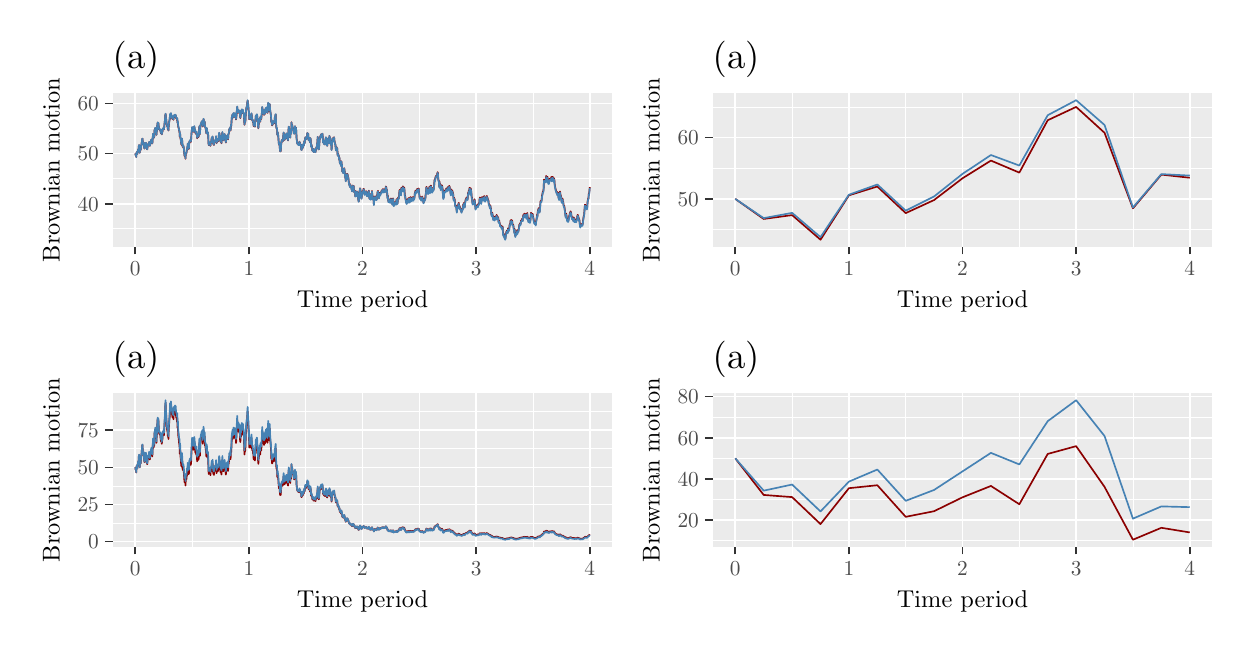
\begin{tikzpicture}[x=1pt,y=1pt]
\definecolor{fillColor}{RGB}{255,255,255}
\path[use as bounding box,fill=fillColor,fill opacity=0.00] (0,0) rectangle (433.62,216.81);
\begin{scope}
\path[clip] (  0.00,108.41) rectangle (216.81,216.81);
\definecolor{drawColor}{RGB}{255,255,255}
\definecolor{fillColor}{RGB}{255,255,255}

\path[draw=drawColor,line width= 0.6pt,line join=round,line cap=round,fill=fillColor] (  0.00,108.41) rectangle (216.81,216.81);
\end{scope}
\begin{scope}
\path[clip] ( 30.68,137.66) rectangle (211.31,193.12);
\definecolor{fillColor}{gray}{0.92}

\path[fill=fillColor] ( 30.68,137.66) rectangle (211.31,193.12);
\definecolor{drawColor}{RGB}{255,255,255}

\path[draw=drawColor,line width= 0.3pt,line join=round] ( 30.68,144.11) --
	(211.31,144.11);

\path[draw=drawColor,line width= 0.3pt,line join=round] ( 30.68,162.24) --
	(211.31,162.24);

\path[draw=drawColor,line width= 0.3pt,line join=round] ( 30.68,180.37) --
	(211.31,180.37);

\path[draw=drawColor,line width= 0.3pt,line join=round] ( 59.42,137.66) --
	( 59.42,193.12);

\path[draw=drawColor,line width= 0.3pt,line join=round] (100.47,137.66) --
	(100.47,193.12);

\path[draw=drawColor,line width= 0.3pt,line join=round] (141.52,137.66) --
	(141.52,193.12);

\path[draw=drawColor,line width= 0.3pt,line join=round] (182.57,137.66) --
	(182.57,193.12);

\path[draw=drawColor,line width= 0.6pt,line join=round] ( 30.68,153.17) --
	(211.31,153.17);

\path[draw=drawColor,line width= 0.6pt,line join=round] ( 30.68,171.30) --
	(211.31,171.30);

\path[draw=drawColor,line width= 0.6pt,line join=round] ( 30.68,189.44) --
	(211.31,189.44);

\path[draw=drawColor,line width= 0.6pt,line join=round] ( 38.89,137.66) --
	( 38.89,193.12);

\path[draw=drawColor,line width= 0.6pt,line join=round] ( 79.94,137.66) --
	( 79.94,193.12);

\path[draw=drawColor,line width= 0.6pt,line join=round] (121.00,137.66) --
	(121.00,193.12);

\path[draw=drawColor,line width= 0.6pt,line join=round] (162.05,137.66) --
	(162.05,193.12);

\path[draw=drawColor,line width= 0.6pt,line join=round] (203.10,137.66) --
	(203.10,193.12);
\definecolor{drawColor}{RGB}{139,0,0}

\path[draw=drawColor,line width= 0.6pt,line join=round] ( 38.89,171.30) --
	( 39.01,170.70) --
	( 39.12,170.87) --
	( 39.23,170.08) --
	( 39.35,171.59) --
	( 39.46,171.90) --
	( 39.58,171.11) --
	( 39.69,171.57) --
	( 39.80,172.27) --
	( 39.92,172.83) --
	( 40.03,172.53) --
	( 40.15,174.00) --
	( 40.26,174.38) --
	( 40.37,173.76) --
	( 40.49,171.60) --
	( 40.60,172.68) --
	( 40.72,172.64) --
	( 40.83,172.62) --
	( 40.94,173.53) --
	( 41.06,174.33) --
	( 41.17,174.91) --
	( 41.29,175.83) --
	( 41.40,176.61) --
	( 41.51,176.68) --
	( 41.63,174.68) --
	( 41.74,175.29) --
	( 41.86,175.23) --
	( 41.97,175.07) --
	( 42.08,173.61) --
	( 42.20,173.14) --
	( 42.31,173.54) --
	( 42.43,174.88) --
	( 42.54,174.77) --
	( 42.65,175.15) --
	( 42.77,175.09) --
	( 42.88,173.73) --
	( 43.00,173.32) --
	( 43.11,172.93) --
	( 43.22,172.86) --
	( 43.34,173.93) --
	( 43.45,174.68) --
	( 43.57,174.51) --
	( 43.68,174.26) --
	( 43.79,174.94) --
	( 43.91,175.49) --
	( 44.02,174.80) --
	( 44.14,174.10) --
	( 44.25,174.45) --
	( 44.36,175.21) --
	( 44.48,175.09) --
	( 44.59,175.97) --
	( 44.71,176.36) --
	( 44.82,175.74) --
	( 44.94,176.08) --
	( 45.05,174.95) --
	( 45.16,176.38) --
	( 45.28,178.39) --
	( 45.39,178.01) --
	( 45.51,176.94) --
	( 45.62,177.51) --
	( 45.73,177.37) --
	( 45.85,179.84) --
	( 45.96,179.79) --
	( 46.08,180.51) --
	( 46.19,180.54) --
	( 46.30,179.75) --
	( 46.42,179.94) --
	( 46.53,178.07) --
	( 46.65,179.58) --
	( 46.76,179.73) --
	( 46.87,182.02) --
	( 46.99,182.53) --
	( 47.10,181.76) --
	( 47.22,182.41) --
	( 47.33,181.40) --
	( 47.44,180.08) --
	( 47.56,180.38) --
	( 47.67,179.91) --
	( 47.79,179.90) --
	( 47.90,179.97) --
	( 48.01,179.35) --
	( 48.13,178.76) --
	( 48.24,178.61) --
	( 48.36,179.83) --
	( 48.47,178.25) --
	( 48.58,178.85) --
	( 48.70,179.19) --
	( 48.81,180.30) --
	( 48.93,179.97) --
	( 49.04,180.36) --
	( 49.15,180.63) --
	( 49.27,180.06) --
	( 49.38,181.32) --
	( 49.50,182.56) --
	( 49.61,183.31) --
	( 49.72,185.03) --
	( 49.84,185.64) --
	( 49.95,184.23) --
	( 50.07,183.60) --
	( 50.18,182.28) --
	( 50.29,181.77) --
	( 50.41,181.10) --
	( 50.52,181.14) --
	( 50.64,180.18) --
	( 50.75,180.34) --
	( 50.86,179.64) --
	( 50.98,181.50) --
	( 51.09,182.26) --
	( 51.21,183.23) --
	( 51.32,183.64) --
	( 51.44,185.48) --
	( 51.55,184.78) --
	( 51.66,184.26) --
	( 51.78,185.83) --
	( 51.89,185.11) --
	( 52.01,184.88) --
	( 52.12,184.44) --
	( 52.23,184.08) --
	( 52.35,183.77) --
	( 52.46,184.31) --
	( 52.58,184.11) --
	( 52.69,183.55) --
	( 52.80,185.01) --
	( 52.92,184.77) --
	( 53.03,184.57) --
	( 53.15,184.45) --
	( 53.26,185.23) --
	( 53.37,185.14) --
	( 53.49,185.10) --
	( 53.60,184.34) --
	( 53.72,183.98) --
	( 53.83,184.04) --
	( 53.94,183.40) --
	( 54.06,183.97) --
	( 54.17,182.32) --
	( 54.29,182.65) --
	( 54.40,181.00) --
	( 54.51,180.68) --
	( 54.63,180.12) --
	( 54.74,179.43) --
	( 54.86,179.37) --
	( 54.97,177.39) --
	( 55.08,178.59) --
	( 55.20,176.88) --
	( 55.31,176.41) --
	( 55.43,175.28) --
	( 55.54,174.53) --
	( 55.65,176.61) --
	( 55.77,176.63) --
	( 55.88,175.33) --
	( 56.00,173.70) --
	( 56.11,174.14) --
	( 56.22,174.11) --
	( 56.34,173.80) --
	( 56.45,172.88) --
	( 56.57,171.44) --
	( 56.68,170.41) --
	( 56.79,171.36) --
	( 56.91,170.76) --
	( 57.02,169.45) --
	( 57.14,171.21) --
	( 57.25,171.62) --
	( 57.36,171.38) --
	( 57.48,172.40) --
	( 57.59,173.25) --
	( 57.71,172.64) --
	( 57.82,174.80) --
	( 57.93,174.55) --
	( 58.05,173.14) --
	( 58.16,173.00) --
	( 58.28,173.19) --
	( 58.39,175.47) --
	( 58.51,175.57) --
	( 58.62,176.02) --
	( 58.73,175.94) --
	( 58.85,175.60) --
	( 58.96,175.56) --
	( 59.08,176.34) --
	( 59.19,178.45) --
	( 59.30,179.51) --
	( 59.42,180.77) --
	( 59.53,179.48) --
	( 59.65,180.50) --
	( 59.76,180.73) --
	( 59.87,179.19) --
	( 59.99,179.72) --
	( 60.10,179.55) --
	( 60.22,181.09) --
	( 60.33,180.27) --
	( 60.44,179.82) --
	( 60.56,178.85) --
	( 60.67,178.66) --
	( 60.79,179.07) --
	( 60.90,178.31) --
	( 61.01,179.16) --
	( 61.13,177.91) --
	( 61.24,176.84) --
	( 61.36,178.30) --
	( 61.47,177.26) --
	( 61.58,177.67) --
	( 61.70,177.28) --
	( 61.81,177.69) --
	( 61.93,179.43) --
	( 62.04,181.09) --
	( 62.15,180.73) --
	( 62.27,178.35) --
	( 62.38,180.95) --
	( 62.50,181.65) --
	( 62.61,182.22) --
	( 62.72,182.20) --
	( 62.84,182.74) --
	( 62.95,182.56) --
	( 63.07,183.01) --
	( 63.18,182.57) --
	( 63.29,181.10) --
	( 63.41,182.15) --
	( 63.52,183.78) --
	( 63.64,183.44) --
	( 63.75,182.09) --
	( 63.86,182.77) --
	( 63.98,182.72) --
	( 64.09,180.86) --
	( 64.21,180.86) --
	( 64.32,180.19) --
	( 64.43,179.83) --
	( 64.55,178.62) --
	( 64.66,180.50) --
	( 64.78,180.14) --
	( 64.89,178.47) --
	( 65.00,178.67) --
	( 65.12,178.93) --
	( 65.23,177.91) --
	( 65.35,174.99) --
	( 65.46,174.35) --
	( 65.58,174.91) --
	( 65.69,174.84) --
	( 65.80,174.74) --
	( 65.92,175.29) --
	( 66.03,174.11) --
	( 66.15,175.19) --
	( 66.26,175.18) --
	( 66.37,175.89) --
	( 66.49,176.92) --
	( 66.60,177.15) --
	( 66.72,176.25) --
	( 66.83,177.42) --
	( 66.94,175.40) --
	( 67.06,174.85) --
	( 67.17,174.59) --
	( 67.29,174.42) --
	( 67.40,175.43) --
	( 67.51,175.56) --
	( 67.63,175.97) --
	( 67.74,175.89) --
	( 67.86,175.64) --
	( 67.97,176.33) --
	( 68.08,177.49) --
	( 68.20,175.06) --
	( 68.31,175.63) --
	( 68.43,176.00) --
	( 68.54,175.57) --
	( 68.65,176.52) --
	( 68.77,176.12) --
	( 68.88,175.83) --
	( 69.00,176.69) --
	( 69.11,178.44) --
	( 69.22,178.71) --
	( 69.34,178.27) --
	( 69.45,177.05) --
	( 69.57,176.71) --
	( 69.68,175.76) --
	( 69.79,175.49) --
	( 69.91,175.88) --
	( 70.02,175.03) --
	( 70.14,177.69) --
	( 70.25,177.85) --
	( 70.36,179.01) --
	( 70.48,176.66) --
	( 70.59,177.40) --
	( 70.71,176.07) --
	( 70.82,176.99) --
	( 70.93,177.39) --
	( 71.05,176.97) --
	( 71.16,178.32) --
	( 71.28,177.59) --
	( 71.39,177.00) --
	( 71.50,175.98) --
	( 71.62,175.31) --
	( 71.73,176.25) --
	( 71.85,176.68) --
	( 71.96,177.70) --
	( 72.08,177.29) --
	( 72.19,177.67) --
	( 72.30,177.92) --
	( 72.42,176.46) --
	( 72.53,178.27) --
	( 72.65,178.40) --
	( 72.76,179.19) --
	( 72.87,180.18) --
	( 72.99,180.12) --
	( 73.10,179.80) --
	( 73.22,180.73) --
	( 73.33,179.62) --
	( 73.44,181.70) --
	( 73.56,181.28) --
	( 73.67,183.05) --
	( 73.79,184.69) --
	( 73.90,184.77) --
	( 74.01,185.39) --
	( 74.13,184.26) --
	( 74.24,184.61) --
	( 74.36,185.75) --
	( 74.47,185.86) --
	( 74.58,185.35) --
	( 74.70,184.62) --
	( 74.81,184.58) --
	( 74.93,185.75) --
	( 75.04,185.21) --
	( 75.15,185.07) --
	( 75.27,183.65) --
	( 75.38,184.18) --
	( 75.50,185.61) --
	( 75.61,187.27) --
	( 75.72,188.19) --
	( 75.84,186.08) --
	( 75.95,186.62) --
	( 76.07,187.12) --
	( 76.18,186.72) --
	( 76.29,186.90) --
	( 76.41,185.93) --
	( 76.52,186.68) --
	( 76.64,186.31) --
	( 76.75,184.57) --
	( 76.86,184.17) --
	( 76.98,185.66) --
	( 77.09,185.29) --
	( 77.21,186.09) --
	( 77.32,187.14) --
	( 77.43,187.14) --
	( 77.55,186.74) --
	( 77.66,186.14) --
	( 77.78,186.96) --
	( 77.89,185.77) --
	( 78.00,186.04) --
	( 78.12,185.71) --
	( 78.23,183.23) --
	( 78.35,181.71) --
	( 78.46,182.69) --
	( 78.57,182.48) --
	( 78.69,183.34) --
	( 78.80,185.39) --
	( 78.92,187.03) --
	( 79.03,187.78) --
	( 79.15,188.21) --
	( 79.26,187.98) --
	( 79.37,189.78) --
	( 79.49,190.46) --
	( 79.60,189.10) --
	( 79.72,188.92) --
	( 79.83,186.75) --
	( 79.94,186.52) --
	( 80.06,183.66) --
	( 80.17,185.09) --
	( 80.29,184.39) --
	( 80.40,183.91) --
	( 80.51,183.72) --
	( 80.63,184.39) --
	( 80.74,185.12) --
	( 80.86,185.75) --
	( 80.97,185.11) --
	( 81.08,183.61) --
	( 81.20,183.19) --
	( 81.31,183.48) --
	( 81.43,182.59) --
	( 81.54,182.51) --
	( 81.65,181.26) --
	( 81.77,181.24) --
	( 81.88,181.37) --
	( 82.00,181.21) --
	( 82.11,181.03) --
	( 82.22,182.91) --
	( 82.34,183.73) --
	( 82.45,184.94) --
	( 82.57,183.92) --
	( 82.68,184.10) --
	( 82.79,185.36) --
	( 82.91,185.29) --
	( 83.02,182.96) --
	( 83.14,183.33) --
	( 83.25,181.28) --
	( 83.36,180.42) --
	( 83.48,181.82) --
	( 83.59,182.47) --
	( 83.71,183.64) --
	( 83.82,183.97) --
	( 83.93,183.84) --
	( 84.05,182.84) --
	( 84.16,184.56) --
	( 84.28,184.61) --
	( 84.39,183.82) --
	( 84.50,184.76) --
	( 84.62,185.94) --
	( 84.73,188.06) --
	( 84.85,187.37) --
	( 84.96,186.93) --
	( 85.07,186.45) --
	( 85.19,186.03) --
	( 85.30,185.62) --
	( 85.42,185.29) --
	( 85.53,186.88) --
	( 85.65,186.10) --
	( 85.76,185.66) --
	( 85.87,186.38) --
	( 85.99,187.64) --
	( 86.10,186.76) --
	( 86.22,186.19) --
	( 86.33,186.77) --
	( 86.44,187.91) --
	( 86.56,187.62) --
	( 86.67,186.01) --
	( 86.79,187.92) --
	( 86.90,189.55) --
	( 87.01,188.73) --
	( 87.13,188.65) --
	( 87.24,186.66) --
	( 87.36,187.29) --
	( 87.47,189.12) --
	( 87.58,187.25) --
	( 87.70,186.38) --
	( 87.81,185.66) --
	( 87.93,184.90) --
	( 88.04,182.68) --
	( 88.15,183.22) --
	( 88.27,181.57) --
	( 88.38,181.54) --
	( 88.50,182.16) --
	( 88.61,181.95) --
	( 88.72,182.90) --
	( 88.84,182.87) --
	( 88.95,182.16) --
	( 89.07,182.85) --
	( 89.18,182.38) --
	( 89.29,184.29) --
	( 89.41,184.27) --
	( 89.52,185.20) --
	( 89.64,185.42) --
	( 89.75,182.14) --
	( 89.86,180.69) --
	( 89.98,180.23) --
	( 90.09,180.48) --
	( 90.21,178.04) --
	( 90.32,179.02) --
	( 90.43,178.39) --
	( 90.55,177.62) --
	( 90.66,176.03) --
	( 90.78,174.58) --
	( 90.89,174.63) --
	( 91.00,175.13) --
	( 91.12,173.06) --
	( 91.23,172.08) --
	( 91.35,172.59) --
	( 91.46,172.15) --
	( 91.57,174.26) --
	( 91.69,175.49) --
	( 91.80,176.08) --
	( 91.92,176.08) --
	( 92.03,176.36) --
	( 92.14,175.64) --
	( 92.26,176.27) --
	( 92.37,177.76) --
	( 92.49,178.87) --
	( 92.60,178.03) --
	( 92.72,176.38) --
	( 92.83,176.26) --
	( 92.94,176.70) --
	( 93.06,178.07) --
	( 93.17,176.72) --
	( 93.29,177.09) --
	( 93.40,177.32) --
	( 93.51,178.54) --
	( 93.63,178.51) --
	( 93.74,178.13) --
	( 93.86,176.96) --
	( 93.97,176.43) --
	( 94.08,176.06) --
	( 94.20,178.44) --
	( 94.31,180.99) --
	( 94.43,180.81) --
	( 94.54,179.71) --
	( 94.65,177.67) --
	( 94.77,178.19) --
	( 94.88,177.07) --
	( 95.00,179.41) --
	( 95.11,178.49) --
	( 95.22,178.60) --
	( 95.34,182.61) --
	( 95.45,181.42) --
	( 95.57,181.74) --
	( 95.68,180.56) --
	( 95.79,180.92) --
	( 95.91,180.00) --
	( 96.02,180.07) --
	( 96.14,179.76) --
	( 96.25,178.52) --
	( 96.36,178.53) --
	( 96.48,179.55) --
	( 96.59,181.22) --
	( 96.71,179.77) --
	( 96.82,179.51) --
	( 96.93,180.72) --
	( 97.05,179.54) --
	( 97.16,176.94) --
	( 97.28,175.99) --
	( 97.39,175.01) --
	( 97.50,175.05) --
	( 97.62,174.65) --
	( 97.73,174.87) --
	( 97.85,174.45) --
	( 97.96,174.81) --
	( 98.07,174.45) --
	( 98.19,175.63) --
	( 98.30,174.89) --
	( 98.42,175.17) --
	( 98.53,174.29) --
	( 98.64,174.49) --
	( 98.76,174.43) --
	( 98.87,172.78) --
	( 98.99,172.63) --
	( 99.10,173.78) --
	( 99.22,174.45) --
	( 99.33,174.58) --
	( 99.44,173.40) --
	( 99.56,174.55) --
	( 99.67,174.62) --
	( 99.79,174.17) --
	( 99.90,175.80) --
	(100.01,175.02) --
	(100.13,175.32) --
	(100.24,176.60) --
	(100.36,177.21) --
	(100.47,176.89) --
	(100.58,176.46) --
	(100.70,176.82) --
	(100.81,177.33) --
	(100.93,177.35) --
	(101.04,178.70) --
	(101.15,178.62) --
	(101.27,177.90) --
	(101.38,178.44) --
	(101.50,176.19) --
	(101.61,176.58) --
	(101.72,177.08) --
	(101.84,176.85) --
	(101.95,175.72) --
	(102.07,175.32) --
	(102.18,176.87) --
	(102.29,176.11) --
	(102.41,173.79) --
	(102.52,174.59) --
	(102.64,174.09) --
	(102.75,173.58) --
	(102.86,172.39) --
	(102.98,172.37) --
	(103.09,173.04) --
	(103.21,172.47) --
	(103.32,171.87) --
	(103.43,172.93) --
	(103.55,172.68) --
	(103.66,172.52) --
	(103.78,171.92) --
	(103.89,172.78) --
	(104.00,171.82) --
	(104.12,172.63) --
	(104.23,173.41) --
	(104.35,172.95) --
	(104.46,173.77) --
	(104.57,174.74) --
	(104.69,175.31) --
	(104.80,177.34) --
	(104.92,175.36) --
	(105.03,174.20) --
	(105.14,172.85) --
	(105.26,173.00) --
	(105.37,174.55) --
	(105.49,176.22) --
	(105.60,176.71) --
	(105.71,177.60) --
	(105.83,177.45) --
	(105.94,177.92) --
	(106.06,178.30) --
	(106.17,177.52) --
	(106.29,177.21) --
	(106.40,177.07) --
	(106.51,178.49) --
	(106.63,177.42) --
	(106.74,175.28) --
	(106.86,176.05) --
	(106.97,175.23) --
	(107.08,174.79) --
	(107.20,175.68) --
	(107.31,174.92) --
	(107.43,174.57) --
	(107.54,176.07) --
	(107.65,176.60) --
	(107.77,177.14) --
	(107.88,177.00) --
	(108.00,175.84) --
	(108.11,174.35) --
	(108.22,174.12) --
	(108.34,176.11) --
	(108.45,176.33) --
	(108.57,176.49) --
	(108.68,176.82) --
	(108.79,176.43) --
	(108.91,175.02) --
	(109.02,177.71) --
	(109.14,177.27) --
	(109.25,176.97) --
	(109.36,175.16) --
	(109.48,174.91) --
	(109.59,174.65) --
	(109.71,174.40) --
	(109.82,172.64) --
	(109.93,174.38) --
	(110.05,176.14) --
	(110.16,176.83) --
	(110.28,175.71) --
	(110.39,176.43) --
	(110.50,176.17) --
	(110.62,175.85) --
	(110.73,177.22) --
	(110.85,175.97) --
	(110.96,175.45) --
	(111.07,174.72) --
	(111.19,174.74) --
	(111.30,173.18) --
	(111.42,172.49) --
	(111.53,173.19) --
	(111.64,173.64) --
	(111.76,172.68) --
	(111.87,173.22) --
	(111.99,170.87) --
	(112.10,170.54) --
	(112.21,171.22) --
	(112.33,170.58) --
	(112.44,170.54) --
	(112.56,169.04) --
	(112.67,169.83) --
	(112.79,168.10) --
	(112.90,167.80) --
	(113.01,167.56) --
	(113.13,167.61) --
	(113.24,166.86) --
	(113.36,168.53) --
	(113.47,167.21) --
	(113.58,167.44) --
	(113.70,164.78) --
	(113.81,164.78) --
	(113.93,165.23) --
	(114.04,164.26) --
	(114.15,164.88) --
	(114.27,165.17) --
	(114.38,166.04) --
	(114.50,165.28) --
	(114.61,164.42) --
	(114.72,162.86) --
	(114.84,162.58) --
	(114.95,161.43) --
	(115.07,162.01) --
	(115.18,162.07) --
	(115.29,163.96) --
	(115.41,162.95) --
	(115.52,163.97) --
	(115.64,163.51) --
	(115.75,162.24) --
	(115.86,162.73) --
	(115.98,161.50) --
	(116.09,160.60) --
	(116.21,159.98) --
	(116.32,160.15) --
	(116.43,159.31) --
	(116.55,160.21) --
	(116.66,159.20) --
	(116.78,159.38) --
	(116.89,159.49) --
	(117.00,158.61) --
	(117.12,158.25) --
	(117.23,157.71) --
	(117.35,158.49) --
	(117.46,159.77) --
	(117.57,158.91) --
	(117.69,159.67) --
	(117.80,159.61) --
	(117.92,157.98) --
	(118.03,157.36) --
	(118.14,157.73) --
	(118.26,157.85) --
	(118.37,155.88) --
	(118.49,156.34) --
	(118.60,156.86) --
	(118.71,156.61) --
	(118.83,156.04) --
	(118.94,157.62) --
	(119.06,157.54) --
	(119.17,157.53) --
	(119.28,156.62) --
	(119.40,155.54) --
	(119.51,154.35) --
	(119.63,154.02) --
	(119.74,155.07) --
	(119.86,156.46) --
	(119.97,157.72) --
	(120.08,158.77) --
	(120.20,158.57) --
	(120.31,157.57) --
	(120.43,157.30) --
	(120.54,155.37) --
	(120.65,155.12) --
	(120.77,156.43) --
	(120.88,156.53) --
	(121.00,157.41) --
	(121.11,157.80) --
	(121.22,157.17) --
	(121.34,158.58) --
	(121.45,158.51) --
	(121.57,157.71) --
	(121.68,157.76) --
	(121.79,156.54) --
	(121.91,157.23) --
	(122.02,157.63) --
	(122.14,157.34) --
	(122.25,156.94) --
	(122.36,157.69) --
	(122.48,156.83) --
	(122.59,156.04) --
	(122.71,156.37) --
	(122.82,156.01) --
	(122.93,156.74) --
	(123.05,156.58) --
	(123.16,157.54) --
	(123.28,157.94) --
	(123.39,156.12) --
	(123.50,155.06) --
	(123.62,156.07) --
	(123.73,156.62) --
	(123.85,155.85) --
	(123.96,154.78) --
	(124.07,155.59) --
	(124.19,154.95) --
	(124.30,156.37) --
	(124.42,157.79) --
	(124.53,156.61) --
	(124.64,155.93) --
	(124.76,154.94) --
	(124.87,155.46) --
	(124.99,154.45) --
	(125.10,152.88) --
	(125.21,154.43) --
	(125.33,155.21) --
	(125.44,155.85) --
	(125.56,155.33) --
	(125.67,155.31) --
	(125.78,155.80) --
	(125.90,154.79) --
	(126.01,154.68) --
	(126.13,154.82) --
	(126.24,156.15) --
	(126.36,156.66) --
	(126.47,157.69) --
	(126.58,157.80) --
	(126.70,156.89) --
	(126.81,156.62) --
	(126.93,155.29) --
	(127.04,156.02) --
	(127.15,157.15) --
	(127.27,157.10) --
	(127.38,156.31) --
	(127.50,157.17) --
	(127.61,157.28) --
	(127.72,156.97) --
	(127.84,157.87) --
	(127.95,157.25) --
	(128.07,158.18) --
	(128.18,157.49) --
	(128.29,157.80) --
	(128.41,158.53) --
	(128.52,157.43) --
	(128.64,157.75) --
	(128.75,157.66) --
	(128.86,158.20) --
	(128.98,157.56) --
	(129.09,157.48) --
	(129.21,158.61) --
	(129.32,158.74) --
	(129.43,159.42) --
	(129.55,159.23) --
	(129.66,158.38) --
	(129.78,158.36) --
	(129.89,157.36) --
	(130.00,155.29) --
	(130.12,156.21) --
	(130.23,155.34) --
	(130.35,153.92) --
	(130.46,154.68) --
	(130.57,154.67) --
	(130.69,154.20) --
	(130.80,154.06) --
	(130.92,153.73) --
	(131.03,154.49) --
	(131.14,155.06) --
	(131.26,153.71) --
	(131.37,153.98) --
	(131.49,154.54) --
	(131.60,155.06) --
	(131.71,153.18) --
	(131.83,152.99) --
	(131.94,154.51) --
	(132.06,155.13) --
	(132.17,153.80) --
	(132.28,152.52) --
	(132.40,152.89) --
	(132.51,152.76) --
	(132.63,153.49) --
	(132.74,153.71) --
	(132.85,153.77) --
	(132.97,153.90) --
	(133.08,154.03) --
	(133.20,153.05) --
	(133.31,154.86) --
	(133.43,153.76) --
	(133.54,153.74) --
	(133.65,153.32) --
	(133.77,154.71) --
	(133.88,155.50) --
	(134.00,155.05) --
	(134.11,155.21) --
	(134.22,156.13) --
	(134.34,157.92) --
	(134.45,158.16) --
	(134.57,157.31) --
	(134.68,156.52) --
	(134.79,158.13) --
	(134.91,156.46) --
	(135.02,158.93) --
	(135.14,158.72) --
	(135.25,158.34) --
	(135.36,158.46) --
	(135.48,159.23) --
	(135.59,159.47) --
	(135.71,157.86) --
	(135.82,158.15) --
	(135.93,158.51) --
	(136.05,159.05) --
	(136.16,158.20) --
	(136.28,156.28) --
	(136.39,156.02) --
	(136.50,155.27) --
	(136.62,154.66) --
	(136.73,153.92) --
	(136.85,153.61) --
	(136.96,153.36) --
	(137.07,153.97) --
	(137.19,154.73) --
	(137.30,154.11) --
	(137.42,153.87) --
	(137.53,154.14) --
	(137.64,155.23) --
	(137.76,155.18) --
	(137.87,153.86) --
	(137.99,154.03) --
	(138.10,153.94) --
	(138.21,155.31) --
	(138.33,155.58) --
	(138.44,155.09) --
	(138.56,154.74) --
	(138.67,154.34) --
	(138.78,154.48) --
	(138.90,154.61) --
	(139.01,155.33) --
	(139.13,155.58) --
	(139.24,155.28) --
	(139.35,154.54) --
	(139.47,155.03) --
	(139.58,154.98) --
	(139.70,155.12) --
	(139.81,155.99) --
	(139.93,157.39) --
	(140.04,156.62) --
	(140.15,157.94) --
	(140.27,157.23) --
	(140.38,157.44) --
	(140.50,157.62) --
	(140.61,157.39) --
	(140.72,158.52) --
	(140.84,157.98) --
	(140.95,158.51) --
	(141.07,158.50) --
	(141.18,157.73) --
	(141.29,158.72) --
	(141.41,157.02) --
	(141.52,156.59) --
	(141.64,155.36) --
	(141.75,155.51) --
	(141.86,155.72) --
	(141.98,154.83) --
	(142.09,155.34) --
	(142.21,154.53) --
	(142.32,155.04) --
	(142.43,155.22) --
	(142.55,155.78) --
	(142.66,155.04) --
	(142.78,155.11) --
	(142.89,154.74) --
	(143.00,153.60) --
	(143.12,153.71) --
	(143.23,155.09) --
	(143.35,154.58) --
	(143.46,154.42) --
	(143.57,154.95) --
	(143.69,154.98) --
	(143.80,156.51) --
	(143.92,157.10) --
	(144.03,158.99) --
	(144.14,159.27) --
	(144.26,158.33) --
	(144.37,158.67) --
	(144.49,157.91) --
	(144.60,157.09) --
	(144.71,156.94) --
	(144.83,157.69) --
	(144.94,157.96) --
	(145.06,158.62) --
	(145.17,159.38) --
	(145.28,159.23) --
	(145.40,157.26) --
	(145.51,157.90) --
	(145.63,159.68) --
	(145.74,159.73) --
	(145.85,158.60) --
	(145.97,158.30) --
	(146.08,157.53) --
	(146.20,157.49) --
	(146.31,158.04) --
	(146.42,158.74) --
	(146.54,158.93) --
	(146.65,158.16) --
	(146.77,158.82) --
	(146.88,159.94) --
	(147.00,161.84) --
	(147.11,161.41) --
	(147.22,161.81) --
	(147.34,162.84) --
	(147.45,162.73) --
	(147.57,163.18) --
	(147.68,163.36) --
	(147.79,163.24) --
	(147.91,163.39) --
	(148.02,164.23) --
	(148.14,164.58) --
	(148.25,164.17) --
	(148.36,162.21) --
	(148.48,161.53) --
	(148.59,161.51) --
	(148.71,159.39) --
	(148.82,161.24) --
	(148.93,159.98) --
	(149.05,159.01) --
	(149.16,160.22) --
	(149.28,158.40) --
	(149.39,159.00) --
	(149.50,158.72) --
	(149.62,159.09) --
	(149.73,159.81) --
	(149.85,159.01) --
	(149.96,158.43) --
	(150.07,156.00) --
	(150.19,155.24) --
	(150.30,155.54) --
	(150.42,155.93) --
	(150.53,157.55) --
	(150.64,157.60) --
	(150.76,157.97) --
	(150.87,158.03) --
	(150.99,157.63) --
	(151.10,158.24) --
	(151.21,158.61) --
	(151.33,158.71) --
	(151.44,158.04) --
	(151.56,158.00) --
	(151.67,158.64) --
	(151.78,159.19) --
	(151.90,158.79) --
	(152.01,158.24) --
	(152.13,158.65) --
	(152.24,159.52) --
	(152.35,159.61) --
	(152.47,159.35) --
	(152.58,158.62) --
	(152.70,158.27) --
	(152.81,157.06) --
	(152.92,156.50) --
	(153.04,157.41) --
	(153.15,158.31) --
	(153.27,157.59) --
	(153.38,157.76) --
	(153.50,157.81) --
	(153.61,156.47) --
	(153.72,157.11) --
	(153.84,155.58) --
	(153.95,154.60) --
	(154.07,155.38) --
	(154.18,154.95) --
	(154.29,154.78) --
	(154.41,153.52) --
	(154.52,152.41) --
	(154.64,152.67) --
	(154.75,152.53) --
	(154.86,152.08) --
	(154.98,151.08) --
	(155.09,150.26) --
	(155.21,151.77) --
	(155.32,151.52) --
	(155.43,152.10) --
	(155.55,152.69) --
	(155.66,153.27) --
	(155.78,153.49) --
	(155.89,152.53) --
	(156.00,151.77) --
	(156.12,152.33) --
	(156.23,151.34) --
	(156.35,151.73) --
	(156.46,151.33) --
	(156.57,151.03) --
	(156.69,150.44) --
	(156.80,150.27) --
	(156.92,150.91) --
	(157.03,151.24) --
	(157.14,151.07) --
	(157.26,151.71) --
	(157.37,152.96) --
	(157.49,152.95) --
	(157.60,153.31) --
	(157.71,153.52) --
	(157.83,152.76) --
	(157.94,152.06) --
	(158.06,153.51) --
	(158.17,154.19) --
	(158.28,154.76) --
	(158.40,154.88) --
	(158.51,155.25) --
	(158.63,155.37) --
	(158.74,155.40) --
	(158.85,155.57) --
	(158.97,154.77) --
	(159.08,156.67) --
	(159.20,157.31) --
	(159.31,157.10) --
	(159.42,158.08) --
	(159.54,157.57) --
	(159.65,158.96) --
	(159.77,158.63) --
	(159.88,156.74) --
	(159.99,157.84) --
	(160.11,158.76) --
	(160.22,158.12) --
	(160.34,156.98) --
	(160.45,155.51) --
	(160.57,155.29) --
	(160.68,153.86) --
	(160.79,153.23) --
	(160.91,153.35) --
	(161.02,154.01) --
	(161.14,153.37) --
	(161.25,153.27) --
	(161.36,153.46) --
	(161.48,154.79) --
	(161.59,154.04) --
	(161.71,152.81) --
	(161.82,151.41) --
	(161.93,151.82) --
	(162.05,151.78) --
	(162.16,152.35) --
	(162.28,152.24) --
	(162.39,152.54) --
	(162.50,152.70) --
	(162.62,152.72) --
	(162.73,152.24) --
	(162.85,153.19) --
	(162.96,152.88) --
	(163.07,153.39) --
	(163.19,153.51) --
	(163.30,154.89) --
	(163.42,155.44) --
	(163.53,155.17) --
	(163.64,155.16) --
	(163.76,155.06) --
	(163.87,153.43) --
	(163.99,154.74) --
	(164.10,155.57) --
	(164.21,154.96) --
	(164.33,155.26) --
	(164.44,155.45) --
	(164.56,154.55) --
	(164.67,155.72) --
	(164.78,155.52) --
	(164.90,155.66) --
	(165.01,155.98) --
	(165.13,155.19) --
	(165.24,154.34) --
	(165.35,154.29) --
	(165.47,154.74) --
	(165.58,154.79) --
	(165.70,155.34) --
	(165.81,155.60) --
	(165.92,156.03) --
	(166.04,154.92) --
	(166.15,155.45) --
	(166.27,154.82) --
	(166.38,154.46) --
	(166.49,154.37) --
	(166.61,153.10) --
	(166.72,153.02) --
	(166.84,152.68) --
	(166.95,152.13) --
	(167.06,151.71) --
	(167.18,152.64) --
	(167.29,151.69) --
	(167.41,151.53) --
	(167.52,149.70) --
	(167.64,149.21) --
	(167.75,148.84) --
	(167.86,149.96) --
	(167.98,149.25) --
	(168.09,148.62) --
	(168.21,147.62) --
	(168.32,147.75) --
	(168.43,148.56) --
	(168.55,147.71) --
	(168.66,147.40) --
	(168.78,148.37) --
	(168.89,147.88) --
	(169.00,148.36) --
	(169.12,148.64) --
	(169.23,147.70) --
	(169.35,148.57) --
	(169.46,149.13) --
	(169.57,148.78) --
	(169.69,148.13) --
	(169.80,147.85) --
	(169.92,148.42) --
	(170.03,148.02) --
	(170.14,146.70) --
	(170.26,146.59) --
	(170.37,147.13) --
	(170.49,146.32) --
	(170.60,146.15) --
	(170.71,145.31) --
	(170.83,145.38) --
	(170.94,145.29) --
	(171.06,145.26) --
	(171.17,144.84) --
	(171.28,144.35) --
	(171.40,144.94) --
	(171.51,145.01) --
	(171.63,144.88) --
	(171.74,142.73) --
	(171.85,141.90) --
	(171.97,142.39) --
	(172.08,142.12) --
	(172.20,141.34) --
	(172.31,141.06) --
	(172.42,140.82) --
	(172.54,140.50) --
	(172.65,140.81) --
	(172.77,141.78) --
	(172.88,142.41) --
	(172.99,143.23) --
	(173.11,143.01) --
	(173.22,143.56) --
	(173.34,142.91) --
	(173.45,142.81) --
	(173.56,144.26) --
	(173.68,144.25) --
	(173.79,144.04) --
	(173.91,143.65) --
	(174.02,144.16) --
	(174.14,145.58) --
	(174.25,145.86) --
	(174.36,145.68) --
	(174.48,147.11) --
	(174.59,146.56) --
	(174.71,147.35) --
	(174.82,147.05) --
	(174.93,146.33) --
	(175.05,147.18) --
	(175.16,145.93) --
	(175.28,145.71) --
	(175.39,145.72) --
	(175.50,145.41) --
	(175.62,144.30) --
	(175.73,143.87) --
	(175.85,142.83) --
	(175.96,144.10) --
	(176.07,142.87) --
	(176.19,141.50) --
	(176.30,141.95) --
	(176.42,142.53) --
	(176.53,142.40) --
	(176.64,142.26) --
	(176.76,142.73) --
	(176.87,143.65) --
	(176.99,142.60) --
	(177.10,143.46) --
	(177.21,143.58) --
	(177.33,143.35) --
	(177.44,144.19) --
	(177.56,144.82) --
	(177.67,145.69) --
	(177.78,145.48) --
	(177.90,146.01) --
	(178.01,146.21) --
	(178.13,145.85) --
	(178.24,147.07) --
	(178.35,147.18) --
	(178.47,147.14) --
	(178.58,147.50) --
	(178.70,147.78) --
	(178.81,147.28) --
	(178.92,147.23) --
	(179.04,149.08) --
	(179.15,149.03) --
	(179.27,148.81) --
	(179.38,149.34) --
	(179.49,149.63) --
	(179.61,149.23) --
	(179.72,148.45) --
	(179.84,149.05) --
	(179.95,149.14) --
	(180.06,149.48) --
	(180.18,149.27) --
	(180.29,148.08) --
	(180.41,148.12) --
	(180.52,149.84) --
	(180.63,148.78) --
	(180.75,148.07) --
	(180.86,147.13) --
	(180.98,146.87) --
	(181.09,147.83) --
	(181.21,147.72) --
	(181.32,147.54) --
	(181.43,146.63) --
	(181.55,146.67) --
	(181.66,147.39) --
	(181.78,149.00) --
	(181.89,149.95) --
	(182.00,149.31) --
	(182.12,148.95) --
	(182.23,149.38) --
	(182.35,149.37) --
	(182.46,149.57) --
	(182.57,148.62) --
	(182.69,148.31) --
	(182.80,147.65) --
	(182.92,146.99) --
	(183.03,146.48) --
	(183.14,146.19) --
	(183.26,146.19) --
	(183.37,146.62) --
	(183.49,146.26) --
	(183.60,145.67) --
	(183.71,146.78) --
	(183.83,147.48) --
	(183.94,147.97) --
	(184.06,149.18) --
	(184.17,148.47) --
	(184.28,149.95) --
	(184.40,150.85) --
	(184.51,151.07) --
	(184.63,151.53) --
	(184.74,151.57) --
	(184.85,151.49) --
	(184.97,150.32) --
	(185.08,150.86) --
	(185.20,152.46) --
	(185.31,154.06) --
	(185.42,154.18) --
	(185.54,154.10) --
	(185.65,154.23) --
	(185.77,155.12) --
	(185.88,156.29) --
	(185.99,156.61) --
	(186.11,157.50) --
	(186.22,157.48) --
	(186.34,157.88) --
	(186.45,158.84) --
	(186.56,161.90) --
	(186.68,161.85) --
	(186.79,161.27) --
	(186.91,161.65) --
	(187.02,161.30) --
	(187.13,161.83) --
	(187.25,162.12) --
	(187.36,163.25) --
	(187.48,162.42) --
	(187.59,161.38) --
	(187.71,162.72) --
	(187.82,162.91) --
	(187.93,162.11) --
	(188.05,161.19) --
	(188.16,160.72) --
	(188.28,161.21) --
	(188.39,160.76) --
	(188.50,161.90) --
	(188.62,162.10) --
	(188.73,162.27) --
	(188.85,162.25) --
	(188.96,161.99) --
	(189.07,161.84) --
	(189.19,162.83) --
	(189.30,161.68) --
	(189.42,162.61) --
	(189.53,162.30) --
	(189.64,162.93) --
	(189.76,162.87) --
	(189.87,161.71) --
	(189.99,162.00) --
	(190.10,161.45) --
	(190.21,162.41) --
	(190.33,161.70) --
	(190.44,160.18) --
	(190.56,159.46) --
	(190.67,158.99) --
	(190.78,158.30) --
	(190.90,158.10) --
	(191.01,157.61) --
	(191.13,157.28) --
	(191.24,157.54) --
	(191.35,156.60) --
	(191.47,157.20) --
	(191.58,157.20) --
	(191.70,157.16) --
	(191.81,155.53) --
	(191.92,155.29) --
	(192.04,154.85) --
	(192.15,155.51) --
	(192.27,156.62) --
	(192.38,157.60) --
	(192.49,156.70) --
	(192.61,156.06) --
	(192.72,155.99) --
	(192.84,155.15) --
	(192.95,153.89) --
	(193.06,154.50) --
	(193.18,154.55) --
	(193.29,155.03) --
	(193.41,154.09) --
	(193.52,153.82) --
	(193.63,152.92) --
	(193.75,152.28) --
	(193.86,152.45) --
	(193.98,151.83) --
	(194.09,151.09) --
	(194.20,150.12) --
	(194.32,149.08) --
	(194.43,148.45) --
	(194.55,149.68) --
	(194.66,149.20) --
	(194.78,148.39) --
	(194.89,147.39) --
	(195.00,147.28) --
	(195.12,147.00) --
	(195.23,147.18) --
	(195.35,146.98) --
	(195.46,147.58) --
	(195.57,148.09) --
	(195.69,148.84) --
	(195.80,149.01) --
	(195.92,149.81) --
	(196.03,149.75) --
	(196.14,150.43) --
	(196.26,150.31) --
	(196.37,149.81) --
	(196.49,148.92) --
	(196.60,148.41) --
	(196.71,147.88) --
	(196.83,148.28) --
	(196.94,148.24) --
	(197.06,147.79) --
	(197.17,147.15) --
	(197.28,148.22) --
	(197.40,148.05) --
	(197.51,147.16) --
	(197.63,146.86) --
	(197.74,146.92) --
	(197.85,147.50) --
	(197.97,147.43) --
	(198.08,147.51) --
	(198.20,146.78) --
	(198.31,147.33) --
	(198.42,147.40) --
	(198.54,147.91) --
	(198.65,149.02) --
	(198.77,149.14) --
	(198.88,148.93) --
	(198.99,148.38) --
	(199.11,147.97) --
	(199.22,147.32) --
	(199.34,147.57) --
	(199.45,146.54) --
	(199.56,145.34) --
	(199.68,144.88) --
	(199.79,145.62) --
	(199.91,145.70) --
	(200.02,145.35) --
	(200.13,145.81) --
	(200.25,145.56) --
	(200.36,145.48) --
	(200.48,145.53) --
	(200.59,146.27) --
	(200.70,147.17) --
	(200.82,148.07) --
	(200.93,148.77) --
	(201.05,149.00) --
	(201.16,150.36) --
	(201.28,151.88) --
	(201.39,152.88) --
	(201.50,152.71) --
	(201.62,151.92) --
	(201.73,152.06) --
	(201.85,151.64) --
	(201.96,151.84) --
	(202.07,151.42) --
	(202.19,152.11) --
	(202.30,153.78) --
	(202.42,154.52) --
	(202.53,155.09) --
	(202.64,155.12) --
	(202.76,156.85) --
	(202.87,156.78) --
	(202.99,157.89) --
	(203.10,159.18);
\definecolor{drawColor}{RGB}{70,130,180}

\path[draw=drawColor,line width= 0.6pt,line join=round] ( 38.89,171.30) --
	( 39.01,170.71) --
	( 39.12,170.88) --
	( 39.23,170.09) --
	( 39.35,171.59) --
	( 39.46,171.90) --
	( 39.58,171.12) --
	( 39.69,171.58) --
	( 39.80,172.29) --
	( 39.92,172.84) --
	( 40.03,172.55) --
	( 40.15,174.01) --
	( 40.26,174.40) --
	( 40.37,173.78) --
	( 40.49,171.61) --
	( 40.60,172.69) --
	( 40.72,172.64) --
	( 40.83,172.63) --
	( 40.94,173.54) --
	( 41.06,174.35) --
	( 41.17,174.93) --
	( 41.29,175.85) --
	( 41.40,176.63) --
	( 41.51,176.71) --
	( 41.63,174.69) --
	( 41.74,175.31) --
	( 41.86,175.25) --
	( 41.97,175.10) --
	( 42.08,173.63) --
	( 42.20,173.16) --
	( 42.31,173.57) --
	( 42.43,174.90) --
	( 42.54,174.80) --
	( 42.65,175.18) --
	( 42.77,175.13) --
	( 42.88,173.76) --
	( 43.00,173.35) --
	( 43.11,172.97) --
	( 43.22,172.91) --
	( 43.34,173.98) --
	( 43.45,174.73) --
	( 43.57,174.57) --
	( 43.68,174.31) --
	( 43.79,175.00) --
	( 43.91,175.56) --
	( 44.02,174.87) --
	( 44.14,174.16) --
	( 44.25,174.52) --
	( 44.36,175.28) --
	( 44.48,175.17) --
	( 44.59,176.05) --
	( 44.71,176.45) --
	( 44.82,175.83) --
	( 44.94,176.17) --
	( 45.05,175.04) --
	( 45.16,176.46) --
	( 45.28,178.46) --
	( 45.39,178.08) --
	( 45.51,177.01) --
	( 45.62,177.59) --
	( 45.73,177.45) --
	( 45.85,179.90) --
	( 45.96,179.86) --
	( 46.08,180.58) --
	( 46.19,180.61) --
	( 46.30,179.83) --
	( 46.42,180.02) --
	( 46.53,178.13) --
	( 46.65,179.64) --
	( 46.76,179.80) --
	( 46.87,182.07) --
	( 46.99,182.58) --
	( 47.10,181.81) --
	( 47.22,182.46) --
	( 47.33,181.46) --
	( 47.44,180.13) --
	( 47.56,180.44) --
	( 47.67,179.97) --
	( 47.79,179.97) --
	( 47.90,180.05) --
	( 48.01,179.43) --
	( 48.13,178.84) --
	( 48.24,178.70) --
	( 48.36,179.92) --
	( 48.47,178.32) --
	( 48.58,178.94) --
	( 48.70,179.28) --
	( 48.81,180.38) --
	( 48.93,180.06) --
	( 49.04,180.45) --
	( 49.15,180.73) --
	( 49.27,180.16) --
	( 49.38,181.43) --
	( 49.50,182.66) --
	( 49.61,183.41) --
	( 49.72,185.13) --
	( 49.84,185.74) --
	( 49.95,184.33) --
	( 50.07,183.70) --
	( 50.18,182.37) --
	( 50.29,181.87) --
	( 50.41,181.21) --
	( 50.52,181.25) --
	( 50.64,180.29) --
	( 50.75,180.45) --
	( 50.86,179.76) --
	( 50.98,181.61) --
	( 51.09,182.37) --
	( 51.21,183.34) --
	( 51.32,183.76) --
	( 51.44,185.59) --
	( 51.55,184.88) --
	( 51.66,184.38) --
	( 51.78,185.94) --
	( 51.89,185.22) --
	( 52.01,184.99) --
	( 52.12,184.56) --
	( 52.23,184.21) --
	( 52.35,183.91) --
	( 52.46,184.44) --
	( 52.58,184.25) --
	( 52.69,183.70) --
	( 52.80,185.15) --
	( 52.92,184.92) --
	( 53.03,184.72) --
	( 53.15,184.61) --
	( 53.26,185.39) --
	( 53.37,185.31) --
	( 53.49,185.27) --
	( 53.60,184.52) --
	( 53.72,184.16) --
	( 53.83,184.23) --
	( 53.94,183.59) --
	( 54.06,184.16) --
	( 54.17,182.51) --
	( 54.29,182.84) --
	( 54.40,181.19) --
	( 54.51,180.87) --
	( 54.63,180.31) --
	( 54.74,179.63) --
	( 54.86,179.57) --
	( 54.97,177.58) --
	( 55.08,178.78) --
	( 55.20,177.06) --
	( 55.31,176.59) --
	( 55.43,175.46) --
	( 55.54,174.71) --
	( 55.65,176.78) --
	( 55.77,176.79) --
	( 55.88,175.49) --
	( 56.00,173.86) --
	( 56.11,174.30) --
	( 56.22,174.28) --
	( 56.34,173.97) --
	( 56.45,173.05) --
	( 56.57,171.61) --
	( 56.68,170.58) --
	( 56.79,171.52) --
	( 56.91,170.93) --
	( 57.02,169.61) --
	( 57.14,171.36) --
	( 57.25,171.77) --
	( 57.36,171.54) --
	( 57.48,172.55) --
	( 57.59,173.41) --
	( 57.71,172.81) --
	( 57.82,174.95) --
	( 57.93,174.69) --
	( 58.05,173.28) --
	( 58.16,173.14) --
	( 58.28,173.34) --
	( 58.39,175.60) --
	( 58.51,175.70) --
	( 58.62,176.16) --
	( 58.73,176.08) --
	( 58.85,175.75) --
	( 58.96,175.71) --
	( 59.08,176.50) --
	( 59.19,178.59) --
	( 59.30,179.65) --
	( 59.42,180.91) --
	( 59.53,179.61) --
	( 59.65,180.64) --
	( 59.76,180.87) --
	( 59.87,179.32) --
	( 59.99,179.86) --
	( 60.10,179.69) --
	( 60.22,181.22) --
	( 60.33,180.41) --
	( 60.44,179.96) --
	( 60.56,178.99) --
	( 60.67,178.81) --
	( 60.79,179.22) --
	( 60.90,178.46) --
	( 61.01,179.32) --
	( 61.13,178.06) --
	( 61.24,176.99) --
	( 61.36,178.45) --
	( 61.47,177.40) --
	( 61.58,177.82) --
	( 61.70,177.43) --
	( 61.81,177.85) --
	( 61.93,179.58) --
	( 62.04,181.23) --
	( 62.15,180.88) --
	( 62.27,178.47) --
	( 62.38,181.04) --
	( 62.50,181.75) --
	( 62.61,182.32) --
	( 62.72,182.31) --
	( 62.84,182.86) --
	( 62.95,182.68) --
	( 63.07,183.13) --
	( 63.18,182.70) --
	( 63.29,181.23) --
	( 63.41,182.27) --
	( 63.52,183.90) --
	( 63.64,183.56) --
	( 63.75,182.20) --
	( 63.86,182.89) --
	( 63.98,182.84) --
	( 64.09,180.98) --
	( 64.21,180.98) --
	( 64.32,180.31) --
	( 64.43,179.96) --
	( 64.55,178.75) --
	( 64.66,180.61) --
	( 64.78,180.26) --
	( 64.89,178.58) --
	( 65.00,178.78) --
	( 65.12,179.05) --
	( 65.23,178.03) --
	( 65.35,175.07) --
	( 65.46,174.43) --
	( 65.58,175.00) --
	( 65.69,174.94) --
	( 65.80,174.84) --
	( 65.92,175.40) --
	( 66.03,174.21) --
	( 66.15,175.29) --
	( 66.26,175.29) --
	( 66.37,175.99) --
	( 66.49,177.03) --
	( 66.60,177.26) --
	( 66.72,176.36) --
	( 66.83,177.54) --
	( 66.94,175.49) --
	( 67.06,174.95) --
	( 67.17,174.70) --
	( 67.29,174.53) --
	( 67.40,175.54) --
	( 67.51,175.68) --
	( 67.63,176.08) --
	( 67.74,176.01) --
	( 67.86,175.77) --
	( 67.97,176.46) --
	( 68.08,177.62) --
	( 68.20,175.17) --
	( 68.31,175.74) --
	( 68.43,176.11) --
	( 68.54,175.68) --
	( 68.65,176.63) --
	( 68.77,176.24) --
	( 68.88,175.96) --
	( 69.00,176.82) --
	( 69.11,178.56) --
	( 69.22,178.83) --
	( 69.34,178.40) --
	( 69.45,177.17) --
	( 69.57,176.84) --
	( 69.68,175.89) --
	( 69.79,175.63) --
	( 69.91,176.02) --
	( 70.02,175.17) --
	( 70.14,177.80) --
	( 70.25,177.96) --
	( 70.36,179.12) --
	( 70.48,176.75) --
	( 70.59,177.50) --
	( 70.71,176.15) --
	( 70.82,177.08) --
	( 70.93,177.48) --
	( 71.05,177.07) --
	( 71.16,178.41) --
	( 71.28,177.69) --
	( 71.39,177.10) --
	( 71.50,176.08) --
	( 71.62,175.41) --
	( 71.73,176.35) --
	( 71.85,176.79) --
	( 71.96,177.81) --
	( 72.08,177.41) --
	( 72.19,177.79) --
	( 72.30,178.04) --
	( 72.42,176.58) --
	( 72.53,178.37) --
	( 72.65,178.51) --
	( 72.76,179.30) --
	( 72.87,180.29) --
	( 72.99,180.24) --
	( 73.10,179.92) --
	( 73.22,180.85) --
	( 73.33,179.75) --
	( 73.44,181.81) --
	( 73.56,181.40) --
	( 73.67,183.15) --
	( 73.79,184.78) --
	( 73.90,184.87) --
	( 74.01,185.50) --
	( 74.13,184.37) --
	( 74.24,184.72) --
	( 74.36,185.86) --
	( 74.47,185.97) --
	( 74.58,185.47) --
	( 74.70,184.74) --
	( 74.81,184.71) --
	( 74.93,185.88) --
	( 75.04,185.34) --
	( 75.15,185.21) --
	( 75.27,183.78) --
	( 75.38,184.32) --
	( 75.50,185.75) --
	( 75.61,187.40) --
	( 75.72,188.32) --
	( 75.84,186.20) --
	( 75.95,186.73) --
	( 76.07,187.24) --
	( 76.18,186.85) --
	( 76.29,187.04) --
	( 76.41,186.07) --
	( 76.52,186.82) --
	( 76.64,186.46) --
	( 76.75,184.71) --
	( 76.86,184.31) --
	( 76.98,185.80) --
	( 77.09,185.43) --
	( 77.21,186.24) --
	( 77.32,187.29) --
	( 77.43,187.29) --
	( 77.55,186.90) --
	( 77.66,186.30) --
	( 77.78,187.13) --
	( 77.89,185.94) --
	( 78.00,186.21) --
	( 78.12,185.89) --
	( 78.23,183.38) --
	( 78.35,181.85) --
	( 78.46,182.83) --
	( 78.57,182.63) --
	( 78.69,183.49) --
	( 78.80,185.53) --
	( 78.92,187.16) --
	( 79.03,187.92) --
	( 79.15,188.35) --
	( 79.26,188.13) --
	( 79.37,189.91) --
	( 79.49,190.60) --
	( 79.60,189.24) --
	( 79.72,189.06) --
	( 79.83,186.87) --
	( 79.94,186.65) --
	( 80.06,183.76) --
	( 80.17,185.19) --
	( 80.29,184.49) --
	( 80.40,184.02) --
	( 80.51,183.83) --
	( 80.63,184.50) --
	( 80.74,185.24) --
	( 80.86,185.87) --
	( 80.97,185.23) --
	( 81.08,183.73) --
	( 81.20,183.31) --
	( 81.31,183.61) --
	( 81.43,182.72) --
	( 81.54,182.64) --
	( 81.65,181.39) --
	( 81.77,181.38) --
	( 81.88,181.52) --
	( 82.00,181.36) --
	( 82.11,181.19) --
	( 82.22,183.05) --
	( 82.34,183.88) --
	( 82.45,185.08) --
	( 82.57,184.07) --
	( 82.68,184.25) --
	( 82.79,185.51) --
	( 82.91,185.45) --
	( 83.02,183.10) --
	( 83.14,183.47) --
	( 83.25,181.41) --
	( 83.36,180.55) --
	( 83.48,181.94) --
	( 83.59,182.59) --
	( 83.71,183.77) --
	( 83.82,184.10) --
	( 83.93,183.98) --
	( 84.05,182.97) --
	( 84.16,184.69) --
	( 84.28,184.74) --
	( 84.39,183.96) --
	( 84.50,184.90) --
	( 84.62,186.08) --
	( 84.73,188.18) --
	( 84.85,187.50) --
	( 84.96,187.06) --
	( 85.07,186.59) --
	( 85.19,186.17) --
	( 85.30,185.76) --
	( 85.42,185.44) --
	( 85.53,187.03) --
	( 85.65,186.25) --
	( 85.76,185.82) --
	( 85.87,186.54) --
	( 85.99,187.79) --
	( 86.10,186.92) --
	( 86.22,186.35) --
	( 86.33,186.93) --
	( 86.44,188.07) --
	( 86.56,187.79) --
	( 86.67,186.18) --
	( 86.79,188.07) --
	( 86.90,189.70) --
	( 87.01,188.88) --
	( 87.13,188.81) --
	( 87.24,186.80) --
	( 87.36,187.44) --
	( 87.47,189.25) --
	( 87.58,187.38) --
	( 87.70,186.51) --
	( 87.81,185.79) --
	( 87.93,185.04) --
	( 88.04,182.80) --
	( 88.15,183.34) --
	( 88.27,181.69) --
	( 88.38,181.66) --
	( 88.50,182.29) --
	( 88.61,182.08) --
	( 88.72,183.03) --
	( 88.84,183.00) --
	( 88.95,182.30) --
	( 89.07,183.00) --
	( 89.18,182.53) --
	( 89.29,184.43) --
	( 89.41,184.41) --
	( 89.52,185.34) --
	( 89.64,185.57) --
	( 89.75,182.25) --
	( 89.86,180.78) --
	( 89.98,180.34) --
	( 90.09,180.59) --
	( 90.21,178.12) --
	( 90.32,179.11) --
	( 90.43,178.48) --
	( 90.55,177.70) --
	( 90.66,176.11) --
	( 90.78,174.65) --
	( 90.89,174.71) --
	( 91.00,175.21) --
	( 91.12,173.12) --
	( 91.23,172.15) --
	( 91.35,172.66) --
	( 91.46,172.22) --
	( 91.57,174.31) --
	( 91.69,175.54) --
	( 91.80,176.14) --
	( 91.92,176.14) --
	( 92.03,176.42) --
	( 92.14,175.71) --
	( 92.26,176.34) --
	( 92.37,177.83) --
	( 92.49,178.94) --
	( 92.60,178.10) --
	( 92.72,176.44) --
	( 92.83,176.33) --
	( 92.94,176.77) --
	( 93.06,178.14) --
	( 93.17,176.78) --
	( 93.29,177.15) --
	( 93.40,177.39) --
	( 93.51,178.61) --
	( 93.63,178.58) --
	( 93.74,178.21) --
	( 93.86,177.03) --
	( 93.97,176.51) --
	( 94.08,176.14) --
	( 94.20,178.50) --
	( 94.31,181.03) --
	( 94.43,180.85) --
	( 94.54,179.75) --
	( 94.65,177.69) --
	( 94.77,178.21) --
	( 94.88,177.09) --
	( 95.00,179.41) --
	( 95.11,178.49) --
	( 95.22,178.61) --
	( 95.34,182.54) --
	( 95.45,181.35) --
	( 95.57,181.68) --
	( 95.68,180.50) --
	( 95.79,180.86) --
	( 95.91,179.94) --
	( 96.02,180.02) --
	( 96.14,179.71) --
	( 96.25,178.47) --
	( 96.36,178.48) --
	( 96.48,179.51) --
	( 96.59,181.17) --
	( 96.71,179.71) --
	( 96.82,179.45) --
	( 96.93,180.66) --
	( 97.05,179.49) --
	( 97.16,176.85) --
	( 97.28,175.90) --
	( 97.39,174.93) --
	( 97.50,174.98) --
	( 97.62,174.57) --
	( 97.73,174.80) --
	( 97.85,174.38) --
	( 97.96,174.75) --
	( 98.07,174.39) --
	( 98.19,175.57) --
	( 98.30,174.83) --
	( 98.42,175.12) --
	( 98.53,174.24) --
	( 98.64,174.44) --
	( 98.76,174.39) --
	( 98.87,172.73) --
	( 98.99,172.59) --
	( 99.10,173.73) --
	( 99.22,174.40) --
	( 99.33,174.54) --
	( 99.44,173.36) --
	( 99.56,174.51) --
	( 99.67,174.58) --
	( 99.79,174.14) --
	( 99.90,175.76) --
	(100.01,174.98) --
	(100.13,175.29) --
	(100.24,176.57) --
	(100.36,177.17) --
	(100.47,176.86) --
	(100.58,176.44) --
	(100.70,176.80) --
	(100.81,177.32) --
	(100.93,177.34) --
	(101.04,178.68) --
	(101.15,178.61) --
	(101.27,177.89) --
	(101.38,178.44) --
	(101.50,176.17) --
	(101.61,176.56) --
	(101.72,177.07) --
	(101.84,176.84) --
	(101.95,175.71) --
	(102.07,175.31) --
	(102.18,176.86) --
	(102.29,176.10) --
	(102.41,173.76) --
	(102.52,174.55) --
	(102.64,174.06) --
	(102.75,173.55) --
	(102.86,172.36) --
	(102.98,172.34) --
	(103.09,173.02) --
	(103.21,172.45) --
	(103.32,171.86) --
	(103.43,172.91) --
	(103.55,172.67) --
	(103.66,172.52) --
	(103.78,171.91) --
	(103.89,172.78) --
	(104.00,171.81) --
	(104.12,172.63) --
	(104.23,173.41) --
	(104.35,172.95) --
	(104.46,173.78) --
	(104.57,174.75) --
	(104.69,175.32) --
	(104.80,177.34) --
	(104.92,175.34) --
	(105.03,174.17) --
	(105.14,172.82) --
	(105.26,172.98) --
	(105.37,174.52) --
	(105.49,176.18) --
	(105.60,176.68) --
	(105.71,177.57) --
	(105.83,177.42) --
	(105.94,177.90) --
	(106.06,178.28) --
	(106.17,177.50) --
	(106.29,177.20) --
	(106.40,177.06) --
	(106.51,178.48) --
	(106.63,177.41) --
	(106.74,175.25) --
	(106.86,176.02) --
	(106.97,175.20) --
	(107.08,174.76) --
	(107.20,175.66) --
	(107.31,174.90) --
	(107.43,174.56) --
	(107.54,176.04) --
	(107.65,176.58) --
	(107.77,177.12) --
	(107.88,176.99) --
	(108.00,175.83) --
	(108.11,174.33) --
	(108.22,174.11) --
	(108.34,176.08) --
	(108.45,176.30) --
	(108.57,176.47) --
	(108.68,176.81) --
	(108.79,176.42) --
	(108.91,175.00) --
	(109.02,177.67) --
	(109.14,177.23) --
	(109.25,176.93) --
	(109.36,175.11) --
	(109.48,174.86) --
	(109.59,174.61) --
	(109.71,174.36) --
	(109.82,172.60) --
	(109.93,174.33) --
	(110.05,176.07) --
	(110.16,176.76) --
	(110.28,175.65) --
	(110.39,176.36) --
	(110.50,176.11) --
	(110.62,175.79) --
	(110.73,177.16) --
	(110.85,175.91) --
	(110.96,175.40) --
	(111.07,174.67) --
	(111.19,174.69) --
	(111.30,173.13) --
	(111.42,172.44) --
	(111.53,173.13) --
	(111.64,173.59) --
	(111.76,172.63) --
	(111.87,173.17) --
	(111.99,170.80) --
	(112.10,170.48) --
	(112.21,171.15) --
	(112.33,170.52) --
	(112.44,170.49) --
	(112.56,168.98) --
	(112.67,169.77) --
	(112.79,168.03) --
	(112.90,167.73) --
	(113.01,167.50) --
	(113.13,167.55) --
	(113.24,166.80) --
	(113.36,168.46) --
	(113.47,167.14) --
	(113.58,167.37) --
	(113.70,164.68) --
	(113.81,164.68) --
	(113.93,165.13) --
	(114.04,164.16) --
	(114.15,164.79) --
	(114.27,165.08) --
	(114.38,165.95) --
	(114.50,165.19) --
	(114.61,164.32) --
	(114.72,162.76) --
	(114.84,162.48) --
	(114.95,161.32) --
	(115.07,161.91) --
	(115.18,161.97) --
	(115.29,163.85) --
	(115.41,162.83) --
	(115.52,163.86) --
	(115.64,163.40) --
	(115.75,162.12) --
	(115.86,162.62) --
	(115.98,161.38) --
	(116.09,160.48) --
	(116.21,159.86) --
	(116.32,160.04) --
	(116.43,159.20) --
	(116.55,160.09) --
	(116.66,159.09) --
	(116.78,159.27) --
	(116.89,159.39) --
	(117.00,158.50) --
	(117.12,158.15) --
	(117.23,157.61) --
	(117.35,158.39) --
	(117.46,159.67) --
	(117.57,158.80) --
	(117.69,159.57) --
	(117.80,159.50) --
	(117.92,157.87) --
	(118.03,157.25) --
	(118.14,157.62) --
	(118.26,157.74) --
	(118.37,155.75) --
	(118.49,156.21) --
	(118.60,156.74) --
	(118.71,156.49) --
	(118.83,155.92) --
	(118.94,157.49) --
	(119.06,157.42) --
	(119.17,157.41) --
	(119.28,156.50) --
	(119.40,155.42) --
	(119.51,154.22) --
	(119.63,153.89) --
	(119.74,154.94) --
	(119.86,156.32) --
	(119.97,157.57) --
	(120.08,158.63) --
	(120.20,158.43) --
	(120.31,157.42) --
	(120.43,157.16) --
	(120.54,155.21) --
	(120.65,154.96) --
	(120.77,156.26) --
	(120.88,156.37) --
	(121.00,157.25) --
	(121.11,157.64) --
	(121.22,157.01) --
	(121.34,158.41) --
	(121.45,158.35) --
	(121.57,157.55) --
	(121.68,157.61) --
	(121.79,156.37) --
	(121.91,157.06) --
	(122.02,157.47) --
	(122.14,157.18) --
	(122.25,156.79) --
	(122.36,157.54) --
	(122.48,156.68) --
	(122.59,155.89) --
	(122.71,156.22) --
	(122.82,155.86) --
	(122.93,156.60) --
	(123.05,156.44) --
	(123.16,157.39) --
	(123.28,157.80) --
	(123.39,155.97) --
	(123.50,154.90) --
	(123.62,155.91) --
	(123.73,156.46) --
	(123.85,155.69) --
	(123.96,154.62) --
	(124.07,155.43) --
	(124.19,154.79) --
	(124.30,156.20) --
	(124.42,157.61) --
	(124.53,156.43) --
	(124.64,155.75) --
	(124.76,154.76) --
	(124.87,155.28) --
	(124.99,154.26) --
	(125.10,152.68) --
	(125.21,154.22) --
	(125.33,155.00) --
	(125.44,155.64) --
	(125.56,155.12) --
	(125.67,155.11) --
	(125.78,155.60) --
	(125.90,154.58) --
	(126.01,154.48) --
	(126.13,154.62) --
	(126.24,155.94) --
	(126.36,156.46) --
	(126.47,157.48) --
	(126.58,157.60) --
	(126.70,156.69) --
	(126.81,156.42) --
	(126.93,155.09) --
	(127.04,155.82) --
	(127.15,156.94) --
	(127.27,156.89) --
	(127.38,156.10) --
	(127.50,156.97) --
	(127.61,157.08) --
	(127.72,156.77) --
	(127.84,157.67) --
	(127.95,157.05) --
	(128.07,157.98) --
	(128.18,157.29) --
	(128.29,157.61) --
	(128.41,158.34) --
	(128.52,157.24) --
	(128.64,157.56) --
	(128.75,157.47) --
	(128.86,158.02) --
	(128.98,157.37) --
	(129.09,157.30) --
	(129.21,158.42) --
	(129.32,158.56) --
	(129.43,159.24) --
	(129.55,159.06) --
	(129.66,158.20) --
	(129.78,158.20) --
	(129.89,157.19) --
	(130.00,155.09) --
	(130.12,156.01) --
	(130.23,155.15) --
	(130.35,153.71) --
	(130.46,154.48) --
	(130.57,154.47) --
	(130.69,154.00) --
	(130.80,153.86) --
	(130.92,153.53) --
	(131.03,154.30) --
	(131.14,154.87) --
	(131.26,153.51) --
	(131.37,153.78) --
	(131.49,154.35) --
	(131.60,154.87) --
	(131.71,152.97) --
	(131.83,152.79) --
	(131.94,154.29) --
	(132.06,154.92) --
	(132.17,153.57) --
	(132.28,152.29) --
	(132.40,152.66) --
	(132.51,152.53) --
	(132.63,153.26) --
	(132.74,153.49) --
	(132.85,153.55) --
	(132.97,153.69) --
	(133.08,153.82) --
	(133.20,152.84) --
	(133.31,154.63) --
	(133.43,153.53) --
	(133.54,153.51) --
	(133.65,153.09) --
	(133.77,154.47) --
	(133.88,155.26) --
	(134.00,154.82) --
	(134.11,154.98) --
	(134.22,155.89) --
	(134.34,157.67) --
	(134.45,157.92) --
	(134.57,157.07) --
	(134.68,156.27) --
	(134.79,157.88) --
	(134.91,156.19) --
	(135.02,158.63) --
	(135.14,158.41) --
	(135.25,158.04) --
	(135.36,158.17) --
	(135.48,158.93) --
	(135.59,159.18) --
	(135.71,157.56) --
	(135.82,157.85) --
	(135.93,158.21) --
	(136.05,158.75) --
	(136.16,157.90) --
	(136.28,155.96) --
	(136.39,155.71) --
	(136.50,154.96) --
	(136.62,154.35) --
	(136.73,153.61) --
	(136.85,153.30) --
	(136.96,153.06) --
	(137.07,153.67) --
	(137.19,154.43) --
	(137.30,153.81) --
	(137.42,153.57) --
	(137.53,153.85) --
	(137.64,154.94) --
	(137.76,154.89) --
	(137.87,153.56) --
	(137.99,153.74) --
	(138.10,153.65) --
	(138.21,155.01) --
	(138.33,155.28) --
	(138.44,154.79) --
	(138.56,154.45) --
	(138.67,154.05) --
	(138.78,154.20) --
	(138.90,154.34) --
	(139.01,155.05) --
	(139.13,155.30) --
	(139.24,155.01) --
	(139.35,154.27) --
	(139.47,154.77) --
	(139.58,154.72) --
	(139.70,154.86) --
	(139.81,155.73) --
	(139.93,157.12) --
	(140.04,156.35) --
	(140.15,157.66) --
	(140.27,156.96) --
	(140.38,157.17) --
	(140.50,157.35) --
	(140.61,157.13) --
	(140.72,158.26) --
	(140.84,157.71) --
	(140.95,158.25) --
	(141.07,158.24) --
	(141.18,157.48) --
	(141.29,158.46) --
	(141.41,156.75) --
	(141.52,156.32) --
	(141.64,155.09) --
	(141.75,155.24) --
	(141.86,155.45) --
	(141.98,154.56) --
	(142.09,155.07) --
	(142.21,154.26) --
	(142.32,154.77) --
	(142.43,154.96) --
	(142.55,155.52) --
	(142.66,154.78) --
	(142.78,154.85) --
	(142.89,154.49) --
	(143.00,153.34) --
	(143.12,153.46) --
	(143.23,154.83) --
	(143.35,154.32) --
	(143.46,154.16) --
	(143.57,154.70) --
	(143.69,154.73) --
	(143.80,156.25) --
	(143.92,156.84) --
	(144.03,158.71) --
	(144.14,159.00) --
	(144.26,158.06) --
	(144.37,158.40) --
	(144.49,157.64) --
	(144.60,156.82) --
	(144.71,156.67) --
	(144.83,157.42) --
	(144.94,157.70) --
	(145.06,158.36) --
	(145.17,159.12) --
	(145.28,158.97) --
	(145.40,156.98) --
	(145.51,157.63) --
	(145.63,159.39) --
	(145.74,159.44) --
	(145.85,158.31) --
	(145.97,158.01) --
	(146.08,157.25) --
	(146.20,157.21) --
	(146.31,157.76) --
	(146.42,158.47) --
	(146.54,158.66) --
	(146.65,157.89) --
	(146.77,158.55) --
	(146.88,159.66) --
	(147.00,161.55) --
	(147.11,161.12) --
	(147.22,161.53) --
	(147.34,162.55) --
	(147.45,162.45) --
	(147.57,162.90) --
	(147.68,163.09) --
	(147.79,162.97) --
	(147.91,163.12) --
	(148.02,163.96) --
	(148.14,164.32) --
	(148.25,163.91) --
	(148.36,161.94) --
	(148.48,161.25) --
	(148.59,161.23) --
	(148.71,159.09) --
	(148.82,160.93) --
	(148.93,159.66) --
	(149.05,158.69) --
	(149.16,159.90) --
	(149.28,158.06) --
	(149.39,158.66) --
	(149.50,158.38) --
	(149.62,158.76) --
	(149.73,159.48) --
	(149.85,158.68) --
	(149.96,158.10) --
	(150.07,155.64) --
	(150.19,154.88) --
	(150.30,155.18) --
	(150.42,155.58) --
	(150.53,157.18) --
	(150.64,157.24) --
	(150.76,157.61) --
	(150.87,157.67) --
	(150.99,157.28) --
	(151.10,157.88) --
	(151.21,158.26) --
	(151.33,158.37) --
	(151.44,157.70) --
	(151.56,157.67) --
	(151.67,158.30) --
	(151.78,158.86) --
	(151.90,158.46) --
	(152.01,157.91) --
	(152.13,158.33) --
	(152.24,159.19) --
	(152.35,159.29) --
	(152.47,159.03) --
	(152.58,158.30) --
	(152.70,157.96) --
	(152.81,156.74) --
	(152.92,156.18) --
	(153.04,157.09) --
	(153.15,157.99) --
	(153.27,157.27) --
	(153.38,157.45) --
	(153.50,157.50) --
	(153.61,156.15) --
	(153.72,156.80) --
	(153.84,155.26) --
	(153.95,154.27) --
	(154.07,155.05) --
	(154.18,154.62) --
	(154.29,154.45) --
	(154.41,153.19) --
	(154.52,152.07) --
	(154.64,152.34) --
	(154.75,152.21) --
	(154.86,151.76) --
	(154.98,150.75) --
	(155.09,149.94) --
	(155.21,151.43) --
	(155.32,151.19) --
	(155.43,151.77) --
	(155.55,152.36) --
	(155.66,152.94) --
	(155.78,153.16) --
	(155.89,152.20) --
	(156.00,151.44) --
	(156.12,152.00) --
	(156.23,151.01) --
	(156.35,151.40) --
	(156.46,151.00) --
	(156.57,150.71) --
	(156.69,150.12) --
	(156.80,149.95) --
	(156.92,150.60) --
	(157.03,150.93) --
	(157.14,150.76) --
	(157.26,151.40) --
	(157.37,152.65) --
	(157.49,152.64) --
	(157.60,153.00) --
	(157.71,153.21) --
	(157.83,152.46) --
	(157.94,151.76) --
	(158.06,153.20) --
	(158.17,153.88) --
	(158.28,154.45) --
	(158.40,154.57) --
	(158.51,154.95) --
	(158.63,155.07) --
	(158.74,155.10) --
	(158.85,155.28) --
	(158.97,154.48) --
	(159.08,156.36) --
	(159.20,157.00) --
	(159.31,156.80) --
	(159.42,157.77) --
	(159.54,157.26) --
	(159.65,158.65) --
	(159.77,158.32) --
	(159.88,156.41) --
	(159.99,157.51) --
	(160.11,158.43) --
	(160.22,157.79) --
	(160.34,156.64) --
	(160.45,155.16) --
	(160.57,154.95) --
	(160.68,153.51) --
	(160.79,152.88) --
	(160.91,153.01) --
	(161.02,153.66) --
	(161.14,153.03) --
	(161.25,152.93) --
	(161.36,153.13) --
	(161.48,154.45) --
	(161.59,153.70) --
	(161.71,152.46) --
	(161.82,151.05) --
	(161.93,151.47) --
	(162.05,151.42) --
	(162.16,152.00) --
	(162.28,151.89) --
	(162.39,152.19) --
	(162.50,152.36) --
	(162.62,152.38) --
	(162.73,151.91) --
	(162.85,152.86) --
	(162.96,152.55) --
	(163.07,153.06) --
	(163.19,153.18) --
	(163.30,154.55) --
	(163.42,155.11) --
	(163.53,154.84) --
	(163.64,154.83) --
	(163.76,154.73) --
	(163.87,153.09) --
	(163.99,154.40) --
	(164.10,155.23) --
	(164.21,154.62) --
	(164.33,154.92) --
	(164.44,155.11) --
	(164.56,154.22) --
	(164.67,155.38) --
	(164.78,155.18) --
	(164.90,155.33) --
	(165.01,155.65) --
	(165.13,154.86) --
	(165.24,154.01) --
	(165.35,153.97) --
	(165.47,154.42) --
	(165.58,154.47) --
	(165.70,155.02) --
	(165.81,155.29) --
	(165.92,155.72) --
	(166.04,154.60) --
	(166.15,155.13) --
	(166.27,154.51) --
	(166.38,154.15) --
	(166.49,154.07) --
	(166.61,152.79) --
	(166.72,152.71) --
	(166.84,152.37) --
	(166.95,151.83) --
	(167.06,151.41) --
	(167.18,152.34) --
	(167.29,151.39) --
	(167.41,151.23) --
	(167.52,149.38) --
	(167.64,148.89) --
	(167.75,148.53) --
	(167.86,149.64) --
	(167.98,148.93) --
	(168.09,148.30) --
	(168.21,147.30) --
	(168.32,147.43) --
	(168.43,148.24) --
	(168.55,147.39) --
	(168.66,147.09) --
	(168.78,148.05) --
	(168.89,147.56) --
	(169.00,148.04) --
	(169.12,148.32) --
	(169.23,147.39) --
	(169.35,148.25) --
	(169.46,148.82) --
	(169.57,148.46) --
	(169.69,147.81) --
	(169.80,147.54) --
	(169.92,148.11) --
	(170.03,147.71) --
	(170.14,146.38) --
	(170.26,146.28) --
	(170.37,146.82) --
	(170.49,146.00) --
	(170.60,145.84) --
	(170.71,145.00) --
	(170.83,145.07) --
	(170.94,144.98) --
	(171.06,144.96) --
	(171.17,144.54) --
	(171.28,144.06) --
	(171.40,144.64) --
	(171.51,144.71) --
	(171.63,144.59) --
	(171.74,142.41) --
	(171.85,141.58) --
	(171.97,142.07) --
	(172.08,141.80) --
	(172.20,141.02) --
	(172.31,140.74) --
	(172.42,140.50) --
	(172.54,140.18) --
	(172.65,140.50) --
	(172.77,141.46) --
	(172.88,142.10) --
	(172.99,142.91) --
	(173.11,142.69) --
	(173.22,143.25) --
	(173.34,142.60) --
	(173.45,142.50) --
	(173.56,143.94) --
	(173.68,143.93) --
	(173.79,143.72) --
	(173.91,143.33) --
	(174.02,143.85) --
	(174.14,145.26) --
	(174.25,145.54) --
	(174.36,145.36) --
	(174.48,146.78) --
	(174.59,146.23) --
	(174.71,147.02) --
	(174.82,146.72) --
	(174.93,146.01) --
	(175.05,146.85) --
	(175.16,145.59) --
	(175.28,145.38) --
	(175.39,145.39) --
	(175.50,145.09) --
	(175.62,143.97) --
	(175.73,143.54) --
	(175.85,142.50) --
	(175.96,143.76) --
	(176.07,142.52) --
	(176.19,141.14) --
	(176.30,141.58) --
	(176.42,142.17) --
	(176.53,142.04) --
	(176.64,141.91) --
	(176.76,142.38) --
	(176.87,143.29) --
	(176.99,142.24) --
	(177.10,143.09) --
	(177.21,143.22) --
	(177.33,142.99) --
	(177.44,143.83) --
	(177.56,144.46) --
	(177.67,145.32) --
	(177.78,145.12) --
	(177.90,145.66) --
	(178.01,145.86) --
	(178.13,145.50) --
	(178.24,146.71) --
	(178.35,146.82) --
	(178.47,146.78) --
	(178.58,147.15) --
	(178.70,147.43) --
	(178.81,146.93) --
	(178.92,146.89) --
	(179.04,148.72) --
	(179.15,148.67) --
	(179.27,148.46) --
	(179.38,148.98) --
	(179.49,149.27) --
	(179.61,148.88) --
	(179.72,148.10) --
	(179.84,148.71) --
	(179.95,148.79) --
	(180.06,149.14) --
	(180.18,148.93) --
	(180.29,147.73) --
	(180.41,147.78) --
	(180.52,149.48) --
	(180.63,148.42) --
	(180.75,147.71) --
	(180.86,146.76) --
	(180.98,146.50) --
	(181.09,147.47) --
	(181.21,147.36) --
	(181.32,147.18) --
	(181.43,146.27) --
	(181.55,146.32) --
	(181.66,147.04) --
	(181.78,148.63) --
	(181.89,149.57) --
	(182.00,148.94) --
	(182.12,148.57) --
	(182.23,149.01) --
	(182.35,149.00) --
	(182.46,149.20) --
	(182.57,148.25) --
	(182.69,147.95) --
	(182.80,147.28) --
	(182.92,146.63) --
	(183.03,146.13) --
	(183.14,145.84) --
	(183.26,145.83) --
	(183.37,146.27) --
	(183.49,145.92) --
	(183.60,145.32) --
	(183.71,146.43) --
	(183.83,147.13) --
	(183.94,147.62) --
	(184.06,148.82) --
	(184.17,148.12) --
	(184.28,149.58) --
	(184.40,150.48) --
	(184.51,150.70) --
	(184.63,151.17) --
	(184.74,151.21) --
	(184.85,151.13) --
	(184.97,149.95) --
	(185.08,150.50) --
	(185.20,152.08) --
	(185.31,153.67) --
	(185.42,153.80) --
	(185.54,153.71) --
	(185.65,153.86) --
	(185.77,154.74) --
	(185.88,155.90) --
	(185.99,156.23) --
	(186.11,157.12) --
	(186.22,157.10) --
	(186.34,157.50) --
	(186.45,158.47) --
	(186.56,161.47) --
	(186.68,161.42) --
	(186.79,160.85) --
	(186.91,161.23) --
	(187.02,160.88) --
	(187.13,161.42) --
	(187.25,161.71) --
	(187.36,162.84) --
	(187.48,162.01) --
	(187.59,160.97) --
	(187.71,162.30) --
	(187.82,162.50) --
	(187.93,161.70) --
	(188.05,160.78) --
	(188.16,160.31) --
	(188.28,160.81) --
	(188.39,160.36) --
	(188.50,161.49) --
	(188.62,161.70) --
	(188.73,161.87) --
	(188.85,161.85) --
	(188.96,161.60) --
	(189.07,161.45) --
	(189.19,162.44) --
	(189.30,161.28) --
	(189.42,162.21) --
	(189.53,161.91) --
	(189.64,162.54) --
	(189.76,162.49) --
	(189.87,161.33) --
	(189.99,161.62) --
	(190.10,161.07) --
	(190.21,162.03) --
	(190.33,161.32) --
	(190.44,159.79) --
	(190.56,159.08) --
	(190.67,158.60) --
	(190.78,157.92) --
	(190.90,157.72) --
	(191.01,157.24) --
	(191.13,156.90) --
	(191.24,157.17) --
	(191.35,156.23) --
	(191.47,156.83) --
	(191.58,156.83) --
	(191.70,156.80) --
	(191.81,155.16) --
	(191.92,154.92) --
	(192.04,154.48) --
	(192.15,155.15) --
	(192.27,156.24) --
	(192.38,157.23) --
	(192.49,156.33) --
	(192.61,155.69) --
	(192.72,155.62) --
	(192.84,154.78) --
	(192.95,153.52) --
	(193.06,154.13) --
	(193.18,154.18) --
	(193.29,154.66) --
	(193.41,153.72) --
	(193.52,153.45) --
	(193.63,152.55) --
	(193.75,151.92) --
	(193.86,152.09) --
	(193.98,151.47) --
	(194.09,150.73) --
	(194.20,149.76) --
	(194.32,148.71) --
	(194.43,148.09) --
	(194.55,149.30) --
	(194.66,148.83) --
	(194.78,148.02) --
	(194.89,147.02) --
	(195.00,146.91) --
	(195.12,146.64) --
	(195.23,146.81) --
	(195.35,146.61) --
	(195.46,147.22) --
	(195.57,147.73) --
	(195.69,148.48) --
	(195.80,148.65) --
	(195.92,149.46) --
	(196.03,149.40) --
	(196.14,150.08) --
	(196.26,149.96) --
	(196.37,149.46) --
	(196.49,148.57) --
	(196.60,148.06) --
	(196.71,147.53) --
	(196.83,147.94) --
	(196.94,147.90) --
	(197.06,147.45) --
	(197.17,146.82) --
	(197.28,147.88) --
	(197.40,147.71) --
	(197.51,146.82) --
	(197.63,146.52) --
	(197.74,146.58) --
	(197.85,147.17) --
	(197.97,147.11) --
	(198.08,147.19) --
	(198.20,146.45) --
	(198.31,147.01) --
	(198.42,147.08) --
	(198.54,147.60) --
	(198.65,148.69) --
	(198.77,148.82) --
	(198.88,148.62) --
	(198.99,148.07) --
	(199.11,147.65) --
	(199.22,147.01) --
	(199.34,147.27) --
	(199.45,146.23) --
	(199.56,145.02) --
	(199.68,144.56) --
	(199.79,145.30) --
	(199.91,145.38) --
	(200.02,145.04) --
	(200.13,145.50) --
	(200.25,145.26) --
	(200.36,145.18) --
	(200.48,145.23) --
	(200.59,145.97) --
	(200.70,146.87) --
	(200.82,147.77) --
	(200.93,148.46) --
	(201.05,148.70) --
	(201.16,150.05) --
	(201.28,151.55) --
	(201.39,152.55) --
	(201.50,152.38) --
	(201.62,151.59) --
	(201.73,151.74) --
	(201.85,151.32) --
	(201.96,151.53) --
	(202.07,151.11) --
	(202.19,151.80) --
	(202.30,153.45) --
	(202.42,154.19) --
	(202.53,154.77) --
	(202.64,154.80) --
	(202.76,156.51) --
	(202.87,156.45) --
	(202.99,157.55) --
	(203.10,158.84);
\end{scope}
\begin{scope}
\path[clip] (  0.00,  0.00) rectangle (433.62,216.81);
\definecolor{drawColor}{gray}{0.30}

\node[text=drawColor,anchor=base east,inner sep=0pt, outer sep=0pt, scale=  0.77] at ( 25.73,150.52) {40};

\node[text=drawColor,anchor=base east,inner sep=0pt, outer sep=0pt, scale=  0.77] at ( 25.73,168.65) {50};

\node[text=drawColor,anchor=base east,inner sep=0pt, outer sep=0pt, scale=  0.77] at ( 25.73,186.78) {60};
\end{scope}
\begin{scope}
\path[clip] (  0.00,  0.00) rectangle (433.62,216.81);
\definecolor{drawColor}{gray}{0.20}

\path[draw=drawColor,line width= 0.6pt,line join=round] ( 27.93,153.17) --
	( 30.68,153.17);

\path[draw=drawColor,line width= 0.6pt,line join=round] ( 27.93,171.30) --
	( 30.68,171.30);

\path[draw=drawColor,line width= 0.6pt,line join=round] ( 27.93,189.44) --
	( 30.68,189.44);
\end{scope}
\begin{scope}
\path[clip] (  0.00,  0.00) rectangle (433.62,216.81);
\definecolor{drawColor}{gray}{0.20}

\path[draw=drawColor,line width= 0.6pt,line join=round] ( 38.89,134.91) --
	( 38.89,137.66);

\path[draw=drawColor,line width= 0.6pt,line join=round] ( 79.94,134.91) --
	( 79.94,137.66);

\path[draw=drawColor,line width= 0.6pt,line join=round] (121.00,134.91) --
	(121.00,137.66);

\path[draw=drawColor,line width= 0.6pt,line join=round] (162.05,134.91) --
	(162.05,137.66);

\path[draw=drawColor,line width= 0.6pt,line join=round] (203.10,134.91) --
	(203.10,137.66);
\end{scope}
\begin{scope}
\path[clip] (  0.00,  0.00) rectangle (433.62,216.81);
\definecolor{drawColor}{gray}{0.30}

\node[text=drawColor,anchor=base,inner sep=0pt, outer sep=0pt, scale=  0.77] at ( 38.89,127.41) {0};

\node[text=drawColor,anchor=base,inner sep=0pt, outer sep=0pt, scale=  0.77] at ( 79.94,127.41) {1};

\node[text=drawColor,anchor=base,inner sep=0pt, outer sep=0pt, scale=  0.77] at (121.00,127.41) {2};

\node[text=drawColor,anchor=base,inner sep=0pt, outer sep=0pt, scale=  0.77] at (162.05,127.41) {3};

\node[text=drawColor,anchor=base,inner sep=0pt, outer sep=0pt, scale=  0.77] at (203.10,127.41) {4};
\end{scope}
\begin{scope}
\path[clip] (  0.00,  0.00) rectangle (433.62,216.81);
\definecolor{drawColor}{RGB}{0,0,0}

\node[text=drawColor,anchor=base,inner sep=0pt, outer sep=0pt, scale=  0.88] at (121.00,115.85) {Time period};
\end{scope}
\begin{scope}
\path[clip] (  0.00,  0.00) rectangle (433.62,216.81);
\definecolor{drawColor}{RGB}{0,0,0}

\node[text=drawColor,rotate= 90.00,anchor=base,inner sep=0pt, outer sep=0pt, scale=  0.88] at ( 11.56,165.39) {Brownian motion};
\end{scope}
\begin{scope}
\path[clip] (  0.00,  0.00) rectangle (433.62,216.81);
\definecolor{drawColor}{RGB}{0,0,0}

\node[text=drawColor,anchor=base west,inner sep=0pt, outer sep=0pt, scale=  1.32] at ( 30.68,202.22) {(a)};
\end{scope}
\begin{scope}
\path[clip] (216.81,108.41) rectangle (433.62,216.81);
\definecolor{drawColor}{RGB}{255,255,255}
\definecolor{fillColor}{RGB}{255,255,255}

\path[draw=drawColor,line width= 0.6pt,line join=round,line cap=round,fill=fillColor] (216.81,108.41) rectangle (433.62,216.81);
\end{scope}
\begin{scope}
\path[clip] (247.49,137.66) rectangle (428.12,193.12);
\definecolor{fillColor}{gray}{0.92}

\path[fill=fillColor] (247.49,137.66) rectangle (428.12,193.12);
\definecolor{drawColor}{RGB}{255,255,255}

\path[draw=drawColor,line width= 0.3pt,line join=round] (247.49,143.85) --
	(428.12,143.85);

\path[draw=drawColor,line width= 0.3pt,line join=round] (247.49,166.01) --
	(428.12,166.01);

\path[draw=drawColor,line width= 0.3pt,line join=round] (247.49,188.17) --
	(428.12,188.17);

\path[draw=drawColor,line width= 0.3pt,line join=round] (276.23,137.66) --
	(276.23,193.12);

\path[draw=drawColor,line width= 0.3pt,line join=round] (317.28,137.66) --
	(317.28,193.12);

\path[draw=drawColor,line width= 0.3pt,line join=round] (358.33,137.66) --
	(358.33,193.12);

\path[draw=drawColor,line width= 0.3pt,line join=round] (399.38,137.66) --
	(399.38,193.12);

\path[draw=drawColor,line width= 0.6pt,line join=round] (247.49,154.93) --
	(428.12,154.93);

\path[draw=drawColor,line width= 0.6pt,line join=round] (247.49,177.09) --
	(428.12,177.09);

\path[draw=drawColor,line width= 0.6pt,line join=round] (255.70,137.66) --
	(255.70,193.12);

\path[draw=drawColor,line width= 0.6pt,line join=round] (296.75,137.66) --
	(296.75,193.12);

\path[draw=drawColor,line width= 0.6pt,line join=round] (337.81,137.66) --
	(337.81,193.12);

\path[draw=drawColor,line width= 0.6pt,line join=round] (378.86,137.66) --
	(378.86,193.12);

\path[draw=drawColor,line width= 0.6pt,line join=round] (419.91,137.66) --
	(419.91,193.12);
\definecolor{drawColor}{RGB}{139,0,0}

\path[draw=drawColor,line width= 0.6pt,line join=round] (255.70,154.93) --
	(265.96,147.69) --
	(276.23,149.08) --
	(286.49,140.18) --
	(296.75,156.23) --
	(307.02,159.41) --
	(317.28,149.80) --
	(327.54,154.53) --
	(337.81,162.39) --
	(348.07,168.78) --
	(358.33,164.43) --
	(368.59,183.36) --
	(378.86,188.17) --
	(389.12,178.82) --
	(399.38,151.53) --
	(409.65,163.71) --
	(419.91,162.58);
\definecolor{drawColor}{RGB}{70,130,180}

\path[draw=drawColor,line width= 0.6pt,line join=round] (255.70,154.93) --
	(265.96,147.99) --
	(276.23,149.89) --
	(286.49,141.12) --
	(296.75,156.45) --
	(307.02,160.14) --
	(317.28,150.68) --
	(327.54,155.83) --
	(337.81,163.98) --
	(348.07,170.79) --
	(358.33,166.99) --
	(368.59,185.17) --
	(378.86,190.60) --
	(389.12,181.65) --
	(399.38,151.82) --
	(409.65,163.90) --
	(419.91,163.36);
\end{scope}
\begin{scope}
\path[clip] (  0.00,  0.00) rectangle (433.62,216.81);
\definecolor{drawColor}{gray}{0.30}

\node[text=drawColor,anchor=base east,inner sep=0pt, outer sep=0pt, scale=  0.77] at (242.54,152.28) {50};

\node[text=drawColor,anchor=base east,inner sep=0pt, outer sep=0pt, scale=  0.77] at (242.54,174.44) {60};
\end{scope}
\begin{scope}
\path[clip] (  0.00,  0.00) rectangle (433.62,216.81);
\definecolor{drawColor}{gray}{0.20}

\path[draw=drawColor,line width= 0.6pt,line join=round] (244.74,154.93) --
	(247.49,154.93);

\path[draw=drawColor,line width= 0.6pt,line join=round] (244.74,177.09) --
	(247.49,177.09);
\end{scope}
\begin{scope}
\path[clip] (  0.00,  0.00) rectangle (433.62,216.81);
\definecolor{drawColor}{gray}{0.20}

\path[draw=drawColor,line width= 0.6pt,line join=round] (255.70,134.91) --
	(255.70,137.66);

\path[draw=drawColor,line width= 0.6pt,line join=round] (296.75,134.91) --
	(296.75,137.66);

\path[draw=drawColor,line width= 0.6pt,line join=round] (337.81,134.91) --
	(337.81,137.66);

\path[draw=drawColor,line width= 0.6pt,line join=round] (378.86,134.91) --
	(378.86,137.66);

\path[draw=drawColor,line width= 0.6pt,line join=round] (419.91,134.91) --
	(419.91,137.66);
\end{scope}
\begin{scope}
\path[clip] (  0.00,  0.00) rectangle (433.62,216.81);
\definecolor{drawColor}{gray}{0.30}

\node[text=drawColor,anchor=base,inner sep=0pt, outer sep=0pt, scale=  0.77] at (255.70,127.41) {0};

\node[text=drawColor,anchor=base,inner sep=0pt, outer sep=0pt, scale=  0.77] at (296.75,127.41) {1};

\node[text=drawColor,anchor=base,inner sep=0pt, outer sep=0pt, scale=  0.77] at (337.81,127.41) {2};

\node[text=drawColor,anchor=base,inner sep=0pt, outer sep=0pt, scale=  0.77] at (378.86,127.41) {3};

\node[text=drawColor,anchor=base,inner sep=0pt, outer sep=0pt, scale=  0.77] at (419.91,127.41) {4};
\end{scope}
\begin{scope}
\path[clip] (  0.00,  0.00) rectangle (433.62,216.81);
\definecolor{drawColor}{RGB}{0,0,0}

\node[text=drawColor,anchor=base,inner sep=0pt, outer sep=0pt, scale=  0.88] at (337.81,115.85) {Time period};
\end{scope}
\begin{scope}
\path[clip] (  0.00,  0.00) rectangle (433.62,216.81);
\definecolor{drawColor}{RGB}{0,0,0}

\node[text=drawColor,rotate= 90.00,anchor=base,inner sep=0pt, outer sep=0pt, scale=  0.88] at (228.37,165.39) {Brownian motion};
\end{scope}
\begin{scope}
\path[clip] (  0.00,  0.00) rectangle (433.62,216.81);
\definecolor{drawColor}{RGB}{0,0,0}

\node[text=drawColor,anchor=base west,inner sep=0pt, outer sep=0pt, scale=  1.32] at (247.49,202.22) {(a)};
\end{scope}
\begin{scope}
\path[clip] (  0.00,  0.00) rectangle (216.81,108.41);
\definecolor{drawColor}{RGB}{255,255,255}
\definecolor{fillColor}{RGB}{255,255,255}

\path[draw=drawColor,line width= 0.6pt,line join=round,line cap=round,fill=fillColor] (  0.00,  0.00) rectangle (216.81,108.41);
\end{scope}
\begin{scope}
\path[clip] ( 30.68, 29.26) rectangle (211.31, 84.71);
\definecolor{fillColor}{gray}{0.92}

\path[fill=fillColor] ( 30.68, 29.26) rectangle (211.31, 84.71);
\definecolor{drawColor}{RGB}{255,255,255}

\path[draw=drawColor,line width= 0.3pt,line join=round] ( 30.68, 37.81) --
	(211.31, 37.81);

\path[draw=drawColor,line width= 0.3pt,line join=round] ( 30.68, 51.22) --
	(211.31, 51.22);

\path[draw=drawColor,line width= 0.3pt,line join=round] ( 30.68, 64.63) --
	(211.31, 64.63);

\path[draw=drawColor,line width= 0.3pt,line join=round] ( 30.68, 78.04) --
	(211.31, 78.04);

\path[draw=drawColor,line width= 0.3pt,line join=round] ( 59.42, 29.26) --
	( 59.42, 84.71);

\path[draw=drawColor,line width= 0.3pt,line join=round] (100.47, 29.26) --
	(100.47, 84.71);

\path[draw=drawColor,line width= 0.3pt,line join=round] (141.52, 29.26) --
	(141.52, 84.71);

\path[draw=drawColor,line width= 0.3pt,line join=round] (182.57, 29.26) --
	(182.57, 84.71);

\path[draw=drawColor,line width= 0.6pt,line join=round] ( 30.68, 31.10) --
	(211.31, 31.10);

\path[draw=drawColor,line width= 0.6pt,line join=round] ( 30.68, 44.51) --
	(211.31, 44.51);

\path[draw=drawColor,line width= 0.6pt,line join=round] ( 30.68, 57.92) --
	(211.31, 57.92);

\path[draw=drawColor,line width= 0.6pt,line join=round] ( 30.68, 71.33) --
	(211.31, 71.33);

\path[draw=drawColor,line width= 0.6pt,line join=round] ( 38.89, 29.26) --
	( 38.89, 84.71);

\path[draw=drawColor,line width= 0.6pt,line join=round] ( 79.94, 29.26) --
	( 79.94, 84.71);

\path[draw=drawColor,line width= 0.6pt,line join=round] (121.00, 29.26) --
	(121.00, 84.71);

\path[draw=drawColor,line width= 0.6pt,line join=round] (162.05, 29.26) --
	(162.05, 84.71);

\path[draw=drawColor,line width= 0.6pt,line join=round] (203.10, 29.26) --
	(203.10, 84.71);
\definecolor{drawColor}{RGB}{139,0,0}

\path[draw=drawColor,line width= 0.6pt,line join=round] ( 38.89, 57.92) --
	( 39.01, 57.02) --
	( 39.12, 57.23) --
	( 39.23, 56.07) --
	( 39.35, 58.22) --
	( 39.46, 58.66) --
	( 39.58, 57.46) --
	( 39.69, 58.11) --
	( 39.80, 59.14) --
	( 39.92, 59.96) --
	( 40.03, 59.46) --
	( 40.15, 61.77) --
	( 40.26, 62.37) --
	( 40.37, 61.32) --
	( 40.49, 57.95) --
	( 40.60, 59.55) --
	( 40.72, 59.44) --
	( 40.83, 59.38) --
	( 40.94, 60.78) --
	( 41.06, 62.05) --
	( 41.17, 62.99) --
	( 41.29, 64.53) --
	( 41.40, 65.89) --
	( 41.51, 65.97) --
	( 41.63, 62.46) --
	( 41.74, 63.46) --
	( 41.86, 63.32) --
	( 41.97, 63.01) --
	( 42.08, 60.59) --
	( 42.20, 59.81) --
	( 42.31, 60.41) --
	( 42.43, 62.54) --
	( 42.54, 62.33) --
	( 42.65, 62.93) --
	( 42.77, 62.80) --
	( 42.88, 60.54) --
	( 43.00, 59.86) --
	( 43.11, 59.23) --
	( 43.22, 59.10) --
	( 43.34, 60.73) --
	( 43.45, 61.91) --
	( 43.57, 61.60) --
	( 43.68, 61.15) --
	( 43.79, 62.23) --
	( 43.91, 63.12) --
	( 44.02, 61.93) --
	( 44.14, 60.76) --
	( 44.25, 61.30) --
	( 44.36, 62.50) --
	( 44.48, 62.27) --
	( 44.59, 63.71) --
	( 44.71, 64.35) --
	( 44.82, 63.25) --
	( 44.94, 63.79) --
	( 45.05, 61.86) --
	( 45.16, 64.22) --
	( 45.28, 67.82) --
	( 45.39, 67.06) --
	( 45.51, 65.09) --
	( 45.62, 66.08) --
	( 45.73, 65.78) --
	( 45.85, 70.41) --
	( 45.96, 70.27) --
	( 46.08, 71.67) --
	( 46.19, 71.67) --
	( 46.30, 70.06) --
	( 46.42, 70.39) --
	( 46.53, 66.78) --
	( 46.65, 69.59) --
	( 46.76, 69.85) --
	( 46.87, 74.49) --
	( 46.99, 75.52) --
	( 47.10, 73.83) --
	( 47.22, 75.17) --
	( 47.33, 73.00) --
	( 47.44, 70.26) --
	( 47.56, 70.81) --
	( 47.67, 69.84) --
	( 47.79, 69.79) --
	( 47.90, 69.89) --
	( 48.01, 68.65) --
	( 48.13, 67.49) --
	( 48.24, 67.18) --
	( 48.36, 69.44) --
	( 48.47, 66.43) --
	( 48.58, 67.51) --
	( 48.70, 68.10) --
	( 48.81, 70.18) --
	( 48.93, 69.50) --
	( 49.04, 70.20) --
	( 49.15, 70.70) --
	( 49.27, 69.53) --
	( 49.38, 72.00) --
	( 49.50, 74.52) --
	( 49.61, 76.09) --
	( 49.72, 79.95) --
	( 49.84, 81.34) --
	( 49.95, 78.00) --
	( 50.07, 76.54) --
	( 50.18, 73.65) --
	( 50.29, 72.54) --
	( 50.41, 71.15) --
	( 50.52, 71.18) --
	( 50.64, 69.25) --
	( 50.75, 69.52) --
	( 50.86, 68.16) --
	( 50.98, 71.73) --
	( 51.09, 73.23) --
	( 51.21, 75.24) --
	( 51.32, 76.08) --
	( 51.44, 80.18) --
	( 51.55, 78.50) --
	( 51.66, 77.29) --
	( 51.78, 80.85) --
	( 51.89, 79.10) --
	( 52.01, 78.52) --
	( 52.12, 77.48) --
	( 52.23, 76.64) --
	( 52.35, 75.91) --
	( 52.46, 77.03) --
	( 52.58, 76.54) --
	( 52.69, 75.28) --
	( 52.80, 78.46) --
	( 52.92, 77.86) --
	( 53.03, 77.36) --
	( 53.15, 77.05) --
	( 53.26, 78.74) --
	( 53.37, 78.49) --
	( 53.49, 78.33) --
	( 53.60, 76.60) --
	( 53.72, 75.77) --
	( 53.83, 75.85) --
	( 53.94, 74.42) --
	( 54.06, 75.59) --
	( 54.17, 72.11) --
	( 54.29, 72.72) --
	( 54.40, 69.43) --
	( 54.51, 68.78) --
	( 54.63, 67.69) --
	( 54.74, 66.41) --
	( 54.86, 66.25) --
	( 54.97, 62.83) --
	( 55.08, 64.82) --
	( 55.20, 61.94) --
	( 55.31, 61.16) --
	( 55.43, 59.40) --
	( 55.54, 58.26) --
	( 55.65, 61.38) --
	( 55.77, 61.37) --
	( 55.88, 59.34) --
	( 56.00, 56.97) --
	( 56.11, 57.55) --
	( 56.22, 57.49) --
	( 56.34, 57.02) --
	( 56.45, 55.74) --
	( 56.57, 53.85) --
	( 56.68, 52.57) --
	( 56.79, 53.70) --
	( 56.91, 52.94) --
	( 57.02, 51.38) --
	( 57.14, 53.45) --
	( 57.25, 53.92) --
	( 57.36, 53.60) --
	( 57.48, 54.86) --
	( 57.59, 55.96) --
	( 57.71, 55.13) --
	( 57.82, 58.06) --
	( 57.93, 57.66) --
	( 58.05, 55.70) --
	( 58.16, 55.48) --
	( 58.28, 55.72) --
	( 58.39, 58.86) --
	( 58.51, 58.98) --
	( 58.62, 59.62) --
	( 58.73, 59.46) --
	( 58.85, 58.93) --
	( 58.96, 58.84) --
	( 59.08, 59.98) --
	( 59.19, 63.27) --
	( 59.30, 65.01) --
	( 59.42, 67.19) --
	( 59.53, 64.88) --
	( 59.65, 66.62) --
	( 59.76, 66.99) --
	( 59.87, 64.27) --
	( 59.99, 65.15) --
	( 60.10, 64.82) --
	( 60.22, 67.47) --
	( 60.33, 65.99) --
	( 60.44, 65.16) --
	( 60.56, 63.49) --
	( 60.67, 63.14) --
	( 60.79, 63.78) --
	( 60.90, 62.50) --
	( 61.01, 63.86) --
	( 61.13, 61.80) --
	( 61.24, 60.11) --
	( 61.36, 62.36) --
	( 61.47, 60.69) --
	( 61.58, 61.29) --
	( 61.70, 60.65) --
	( 61.81, 61.25) --
	( 61.93, 64.01) --
	( 62.04, 66.84) --
	( 62.15, 66.17) --
	( 62.27, 62.15) --
	( 62.38, 66.47) --
	( 62.50, 67.68) --
	( 62.61, 68.69) --
	( 62.72, 68.61) --
	( 62.84, 69.58) --
	( 62.95, 69.19) --
	( 63.07, 69.99) --
	( 63.18, 69.13) --
	( 63.29, 66.43) --
	( 63.41, 68.26) --
	( 63.52, 71.31) --
	( 63.64, 70.60) --
	( 63.75, 68.03) --
	( 63.86, 69.25) --
	( 63.98, 69.10) --
	( 64.09, 65.74) --
	( 64.21, 65.69) --
	( 64.32, 64.52) --
	( 64.43, 63.88) --
	( 64.55, 61.90) --
	( 64.66, 64.92) --
	( 64.78, 64.29) --
	( 64.89, 61.55) --
	( 65.00, 61.83) --
	( 65.12, 62.21) --
	( 65.23, 60.60) --
	( 65.35, 56.40) --
	( 65.46, 55.52) --
	( 65.58, 56.23) --
	( 65.69, 56.12) --
	( 65.80, 55.96) --
	( 65.92, 56.67) --
	( 66.03, 55.08) --
	( 66.15, 56.48) --
	( 66.26, 56.43) --
	( 66.37, 57.36) --
	( 66.49, 58.79) --
	( 66.60, 59.08) --
	( 66.72, 57.78) --
	( 66.83, 59.42) --
	( 66.94, 56.55) --
	( 67.06, 55.80) --
	( 67.17, 55.44) --
	( 67.29, 55.19) --
	( 67.40, 56.49) --
	( 67.51, 56.63) --
	( 67.63, 57.15) --
	( 67.74, 57.02) --
	( 67.86, 56.65) --
	( 67.97, 57.56) --
	( 68.08, 59.17) --
	( 68.20, 55.80) --
	( 68.31, 56.52) --
	( 68.43, 56.99) --
	( 68.54, 56.38) --
	( 68.65, 57.65) --
	( 68.77, 57.07) --
	( 68.88, 56.65) --
	( 69.00, 57.79) --
	( 69.11, 60.28) --
	( 69.22, 60.66) --
	( 69.34, 59.97) --
	( 69.45, 58.18) --
	( 69.57, 57.67) --
	( 69.68, 56.36) --
	( 69.79, 55.98) --
	( 69.91, 56.47) --
	( 70.02, 55.32) --
	( 70.14, 58.91) --
	( 70.25, 59.10) --
	( 70.36, 60.78) --
	( 70.48, 57.37) --
	( 70.59, 58.38) --
	( 70.71, 56.51) --
	( 70.82, 57.74) --
	( 70.93, 58.26) --
	( 71.05, 57.65) --
	( 71.16, 59.53) --
	( 71.28, 58.46) --
	( 71.39, 57.60) --
	( 71.50, 56.20) --
	( 71.62, 55.30) --
	( 71.73, 56.50) --
	( 71.85, 57.05) --
	( 71.96, 58.43) --
	( 72.08, 57.83) --
	( 72.19, 58.33) --
	( 72.30, 58.64) --
	( 72.42, 56.61) --
	( 72.53, 59.08) --
	( 72.65, 59.24) --
	( 72.76, 60.36) --
	( 72.87, 61.83) --
	( 72.99, 61.70) --
	( 73.10, 61.17) --
	( 73.22, 62.58) --
	( 73.33, 60.85) --
	( 73.44, 64.06) --
	( 73.56, 63.35) --
	( 73.67, 66.24) --
	( 73.79, 69.11) --
	( 73.90, 69.22) --
	( 74.01, 70.32) --
	( 74.13, 68.21) --
	( 74.24, 68.79) --
	( 74.36, 70.87) --
	( 74.47, 71.02) --
	( 74.58, 70.02) --
	( 74.70, 68.65) --
	( 74.81, 68.53) --
	( 74.93, 70.64) --
	( 75.04, 69.59) --
	( 75.15, 69.29) --
	( 75.27, 66.73) --
	( 75.38, 67.61) --
	( 75.50, 70.17) --
	( 75.61, 73.31) --
	( 75.72, 75.11) --
	( 75.84, 70.92) --
	( 75.95, 71.89) --
	( 76.07, 72.82) --
	( 76.18, 72.00) --
	( 76.29, 72.31) --
	( 76.41, 70.42) --
	( 76.52, 71.80) --
	( 76.64, 71.04) --
	( 76.75, 67.82) --
	( 76.86, 67.07) --
	( 76.98, 69.70) --
	( 77.09, 68.97) --
	( 77.21, 70.41) --
	( 77.32, 72.36) --
	( 77.43, 72.31) --
	( 77.55, 71.50) --
	( 77.66, 70.33) --
	( 77.78, 71.83) --
	( 77.89, 69.56) --
	( 78.00, 70.01) --
	( 78.12, 69.37) --
	( 78.23, 65.01) --
	( 78.35, 62.54) --
	( 78.46, 64.05) --
	( 78.57, 63.68) --
	( 78.69, 65.04) --
	( 78.80, 68.54) --
	( 78.92, 71.50) --
	( 79.03, 72.91) --
	( 79.15, 73.70) --
	( 79.26, 73.21) --
	( 79.37, 76.80) --
	( 79.49, 78.19) --
	( 79.60, 75.31) --
	( 79.72, 74.88) --
	( 79.83, 70.62) --
	( 79.94, 70.16) --
	( 80.06, 65.12) --
	( 80.17, 67.51) --
	( 80.29, 66.27) --
	( 80.40, 65.43) --
	( 80.51, 65.08) --
	( 80.63, 66.14) --
	( 80.74, 67.37) --
	( 80.86, 68.42) --
	( 80.97, 67.26) --
	( 81.08, 64.70) --
	( 81.20, 63.98) --
	( 81.31, 64.42) --
	( 81.43, 62.96) --
	( 81.54, 62.80) --
	( 81.65, 60.87) --
	( 81.77, 60.81) --
	( 81.88, 60.97) --
	( 82.00, 60.70) --
	( 82.11, 60.41) --
	( 82.22, 63.22) --
	( 82.34, 64.49) --
	( 82.45, 66.45) --
	( 82.57, 64.73) --
	( 82.68, 64.97) --
	( 82.79, 67.05) --
	( 82.91, 66.89) --
	( 83.02, 63.05) --
	( 83.14, 63.59) --
	( 83.25, 60.44) --
	( 83.36, 59.18) --
	( 83.48, 61.16) --
	( 83.59, 62.11) --
	( 83.71, 63.90) --
	( 83.82, 64.39) --
	( 83.93, 64.15) --
	( 84.05, 62.54) --
	( 84.16, 65.24) --
	( 84.28, 65.28) --
	( 84.39, 63.97) --
	( 84.50, 65.45) --
	( 84.62, 67.40) --
	( 84.73, 71.16) --
	( 84.85, 69.85) --
	( 84.96, 69.01) --
	( 85.07, 68.14) --
	( 85.19, 67.36) --
	( 85.30, 66.62) --
	( 85.42, 66.02) --
	( 85.53, 68.73) --
	( 85.65, 67.32) --
	( 85.76, 66.53) --
	( 85.87, 67.72) --
	( 85.99, 69.91) --
	( 86.10, 68.31) --
	( 86.22, 67.27) --
	( 86.33, 68.23) --
	( 86.44, 70.23) --
	( 86.56, 69.66) --
	( 86.67, 66.81) --
	( 86.79, 70.12) --
	( 86.90, 73.13) --
	( 87.01, 71.53) --
	( 87.13, 71.33) --
	( 87.24, 67.72) --
	( 87.36, 68.78) --
	( 87.47, 72.07) --
	( 87.58, 68.63) --
	( 87.70, 67.07) --
	( 87.81, 65.83) --
	( 87.93, 64.55) --
	( 88.04, 61.11) --
	( 88.15, 61.87) --
	( 88.27, 59.45) --
	( 88.38, 59.37) --
	( 88.50, 60.23) --
	( 88.61, 59.89) --
	( 88.72, 61.23) --
	( 88.84, 61.15) --
	( 88.95, 60.10) --
	( 89.07, 61.06) --
	( 89.18, 60.34) --
	( 89.29, 63.16) --
	( 89.41, 63.09) --
	( 89.52, 64.51) --
	( 89.64, 64.83) --
	( 89.75, 59.84) --
	( 89.86, 57.81) --
	( 89.98, 57.18) --
	( 90.09, 57.47) --
	( 90.21, 54.38) --
	( 90.32, 55.55) --
	( 90.43, 54.75) --
	( 90.55, 53.80) --
	( 90.66, 51.99) --
	( 90.78, 50.42) --
	( 90.89, 50.45) --
	( 91.00, 50.95) --
	( 91.12, 48.85) --
	( 91.23, 47.91) --
	( 91.35, 48.37) --
	( 91.46, 47.94) --
	( 91.57, 49.94) --
	( 91.69, 51.20) --
	( 91.80, 51.81) --
	( 91.92, 51.78) --
	( 92.03, 52.06) --
	( 92.14, 51.27) --
	( 92.26, 51.92) --
	( 92.37, 53.58) --
	( 92.49, 54.86) --
	( 92.60, 53.83) --
	( 92.72, 51.95) --
	( 92.83, 51.80) --
	( 92.94, 52.25) --
	( 93.06, 53.78) --
	( 93.17, 52.23) --
	( 93.29, 52.61) --
	( 93.40, 52.85) --
	( 93.51, 54.23) --
	( 93.63, 54.16) --
	( 93.74, 53.70) --
	( 93.86, 52.35) --
	( 93.97, 51.75) --
	( 94.08, 51.33) --
	( 94.20, 53.96) --
	( 94.31, 57.07) --
	( 94.43, 56.81) --
	( 94.54, 55.40) --
	( 94.65, 52.97) --
	( 94.77, 53.54) --
	( 94.88, 52.26) --
	( 95.00, 54.93) --
	( 95.11, 53.81) --
	( 95.22, 53.91) --
	( 95.34, 58.95) --
	( 95.45, 57.33) --
	( 95.57, 57.72) --
	( 95.68, 56.18) --
	( 95.79, 56.61) --
	( 95.91, 55.43) --
	( 96.02, 55.49) --
	( 96.14, 55.08) --
	( 96.25, 53.60) --
	( 96.36, 53.58) --
	( 96.48, 54.76) --
	( 96.59, 56.79) --
	( 96.71, 54.97) --
	( 96.82, 54.62) --
	( 96.93, 56.07) --
	( 97.05, 54.61) --
	( 97.16, 51.65) --
	( 97.28, 50.63) --
	( 97.39, 49.64) --
	( 97.50, 49.66) --
	( 97.62, 49.24) --
	( 97.73, 49.44) --
	( 97.85, 49.01) --
	( 97.96, 49.34) --
	( 98.07, 48.97) --
	( 98.19, 50.10) --
	( 98.30, 49.35) --
	( 98.42, 49.61) --
	( 98.53, 48.74) --
	( 98.64, 48.91) --
	( 98.76, 48.84) --
	( 98.87, 47.31) --
	( 98.99, 47.16) --
	( 99.10, 48.17) --
	( 99.22, 48.77) --
	( 99.33, 48.88) --
	( 99.44, 47.77) --
	( 99.56, 48.81) --
	( 99.67, 48.86) --
	( 99.79, 48.42) --
	( 99.90, 49.96) --
	(100.01, 49.18) --
	(100.13, 49.45) --
	(100.24, 50.70) --
	(100.36, 51.31) --
	(100.47, 50.95) --
	(100.58, 50.49) --
	(100.70, 50.83) --
	(100.81, 51.35) --
	(100.93, 51.34) --
	(101.04, 52.76) --
	(101.15, 52.66) --
	(101.27, 51.85) --
	(101.38, 52.42) --
	(101.50, 50.05) --
	(101.61, 50.42) --
	(101.72, 50.91) --
	(101.84, 50.65) --
	(101.95, 49.50) --
	(102.07, 49.10) --
	(102.18, 50.60) --
	(102.29, 49.83) --
	(102.41, 47.64) --
	(102.52, 48.34) --
	(102.64, 47.87) --
	(102.75, 47.40) --
	(102.86, 46.37) --
	(102.98, 46.33) --
	(103.09, 46.88) --
	(103.21, 46.38) --
	(103.32, 45.88) --
	(103.43, 46.73) --
	(103.55, 46.51) --
	(103.66, 46.36) --
	(103.78, 45.84) --
	(103.89, 46.54) --
	(104.00, 45.73) --
	(104.12, 46.38) --
	(104.23, 47.02) --
	(104.35, 46.61) --
	(104.46, 47.30) --
	(104.57, 48.14) --
	(104.69, 48.64) --
	(104.80, 50.58) --
	(104.92, 48.65) --
	(105.03, 47.58) --
	(105.14, 46.40) --
	(105.26, 46.52) --
	(105.37, 47.84) --
	(105.49, 49.36) --
	(105.60, 49.81) --
	(105.71, 50.67) --
	(105.83, 50.49) --
	(105.94, 50.95) --
	(106.06, 51.32) --
	(106.17, 50.50) --
	(106.29, 50.18) --
	(106.40, 50.01) --
	(106.51, 51.43) --
	(106.63, 50.32) --
	(106.74, 48.27) --
	(106.86, 48.95) --
	(106.97, 48.18) --
	(107.08, 47.77) --
	(107.20, 48.56) --
	(107.31, 47.85) --
	(107.43, 47.52) --
	(107.54, 48.85) --
	(107.65, 49.33) --
	(107.77, 49.83) --
	(107.88, 49.67) --
	(108.00, 48.57) --
	(108.11, 47.22) --
	(108.22, 47.01) --
	(108.34, 48.75) --
	(108.45, 48.94) --
	(108.57, 49.07) --
	(108.68, 49.36) --
	(108.79, 48.97) --
	(108.91, 47.68) --
	(109.02, 50.16) --
	(109.14, 49.71) --
	(109.25, 49.40) --
	(109.36, 47.72) --
	(109.48, 47.49) --
	(109.59, 47.25) --
	(109.71, 47.01) --
	(109.82, 45.56) --
	(109.93, 46.97) --
	(110.05, 48.49) --
	(110.16, 49.11) --
	(110.28, 48.07) --
	(110.39, 48.69) --
	(110.50, 48.44) --
	(110.62, 48.13) --
	(110.73, 49.37) --
	(110.85, 48.20) --
	(110.96, 47.73) --
	(111.07, 47.08) --
	(111.19, 47.07) --
	(111.30, 45.78) --
	(111.42, 45.23) --
	(111.53, 45.75) --
	(111.64, 46.09) --
	(111.76, 45.32) --
	(111.87, 45.73) --
	(111.99, 43.95) --
	(112.10, 43.70) --
	(112.21, 44.17) --
	(112.33, 43.70) --
	(112.44, 43.66) --
	(112.56, 42.64) --
	(112.67, 43.15) --
	(112.79, 42.01) --
	(112.90, 41.81) --
	(113.01, 41.65) --
	(113.13, 41.67) --
	(113.24, 41.21) --
	(113.36, 42.22) --
	(113.47, 41.40) --
	(113.58, 41.52) --
	(113.70, 40.01) --
	(113.81, 40.00) --
	(113.93, 40.23) --
	(114.04, 39.71) --
	(114.15, 40.03) --
	(114.27, 40.17) --
	(114.38, 40.64) --
	(114.50, 40.21) --
	(114.61, 39.74) --
	(114.72, 38.96) --
	(114.84, 38.82) --
	(114.95, 38.28) --
	(115.07, 38.54) --
	(115.18, 38.56) --
	(115.29, 39.46) --
	(115.41, 38.95) --
	(115.52, 39.44) --
	(115.64, 39.20) --
	(115.75, 38.59) --
	(115.86, 38.81) --
	(115.98, 38.24) --
	(116.09, 37.85) --
	(116.21, 37.58) --
	(116.32, 37.65) --
	(116.43, 37.30) --
	(116.55, 37.65) --
	(116.66, 37.25) --
	(116.78, 37.31) --
	(116.89, 37.35) --
	(117.00, 37.00) --
	(117.12, 36.86) --
	(117.23, 36.65) --
	(117.35, 36.93) --
	(117.46, 37.42) --
	(117.57, 37.08) --
	(117.69, 37.37) --
	(117.80, 37.34) --
	(117.92, 36.71) --
	(118.03, 36.49) --
	(118.14, 36.61) --
	(118.26, 36.65) --
	(118.37, 35.97) --
	(118.49, 36.11) --
	(118.60, 36.28) --
	(118.71, 36.19) --
	(118.83, 36.00) --
	(118.94, 36.53) --
	(119.06, 36.50) --
	(119.17, 36.48) --
	(119.28, 36.17) --
	(119.40, 35.82) --
	(119.51, 35.45) --
	(119.63, 35.34) --
	(119.74, 35.65) --
	(119.86, 36.09) --
	(119.97, 36.51) --
	(120.08, 36.88) --
	(120.20, 36.80) --
	(120.31, 36.44) --
	(120.43, 36.34) --
	(120.54, 35.71) --
	(120.65, 35.63) --
	(120.77, 36.03) --
	(120.88, 36.06) --
	(121.00, 36.35) --
	(121.11, 36.48) --
	(121.22, 36.26) --
	(121.34, 36.74) --
	(121.45, 36.71) --
	(121.57, 36.42) --
	(121.68, 36.44) --
	(121.79, 36.02) --
	(121.91, 36.24) --
	(122.02, 36.37) --
	(122.14, 36.27) --
	(122.25, 36.13) --
	(122.36, 36.38) --
	(122.48, 36.08) --
	(122.59, 35.82) --
	(122.71, 35.92) --
	(122.82, 35.80) --
	(122.93, 36.03) --
	(123.05, 35.97) --
	(123.16, 36.28) --
	(123.28, 36.41) --
	(123.39, 35.81) --
	(123.50, 35.49) --
	(123.62, 35.79) --
	(123.73, 35.95) --
	(123.85, 35.71) --
	(123.96, 35.39) --
	(124.07, 35.62) --
	(124.19, 35.42) --
	(124.30, 35.85) --
	(124.42, 36.30) --
	(124.53, 35.91) --
	(124.64, 35.70) --
	(124.76, 35.40) --
	(124.87, 35.55) --
	(124.99, 35.25) --
	(125.10, 34.82) --
	(125.21, 35.23) --
	(125.33, 35.45) --
	(125.44, 35.64) --
	(125.56, 35.48) --
	(125.67, 35.47) --
	(125.78, 35.61) --
	(125.90, 35.31) --
	(126.01, 35.27) --
	(126.13, 35.31) --
	(126.24, 35.69) --
	(126.36, 35.84) --
	(126.47, 36.17) --
	(126.58, 36.20) --
	(126.70, 35.90) --
	(126.81, 35.81) --
	(126.93, 35.41) --
	(127.04, 35.62) --
	(127.15, 35.96) --
	(127.27, 35.94) --
	(127.38, 35.69) --
	(127.50, 35.95) --
	(127.61, 35.98) --
	(127.72, 35.88) --
	(127.84, 36.16) --
	(127.95, 35.96) --
	(128.07, 36.25) --
	(128.18, 36.02) --
	(128.29, 36.12) --
	(128.41, 36.35) --
	(128.52, 35.99) --
	(128.64, 36.08) --
	(128.75, 36.05) --
	(128.86, 36.22) --
	(128.98, 36.00) --
	(129.09, 35.98) --
	(129.21, 36.34) --
	(129.32, 36.38) --
	(129.43, 36.60) --
	(129.55, 36.53) --
	(129.66, 36.24) --
	(129.78, 36.23) --
	(129.89, 35.90) --
	(130.00, 35.28) --
	(130.12, 35.54) --
	(130.23, 35.29) --
	(130.35, 34.90) --
	(130.46, 35.10) --
	(130.57, 35.09) --
	(130.69, 34.96) --
	(130.80, 34.92) --
	(130.92, 34.83) --
	(131.03, 35.02) --
	(131.14, 35.17) --
	(131.26, 34.81) --
	(131.37, 34.88) --
	(131.49, 35.02) --
	(131.60, 35.15) --
	(131.71, 34.66) --
	(131.83, 34.61) --
	(131.94, 34.99) --
	(132.06, 35.16) --
	(132.17, 34.80) --
	(132.28, 34.49) --
	(132.40, 34.57) --
	(132.51, 34.53) --
	(132.63, 34.71) --
	(132.74, 34.76) --
	(132.85, 34.77) --
	(132.97, 34.80) --
	(133.08, 34.83) --
	(133.20, 34.58) --
	(133.31, 35.03) --
	(133.43, 34.75) --
	(133.54, 34.74) --
	(133.65, 34.63) --
	(133.77, 34.98) --
	(133.88, 35.18) --
	(134.00, 35.06) --
	(134.11, 35.10) --
	(134.22, 35.34) --
	(134.34, 35.87) --
	(134.45, 35.94) --
	(134.57, 35.67) --
	(134.68, 35.43) --
	(134.79, 35.91) --
	(134.91, 35.41) --
	(135.02, 36.15) --
	(135.14, 36.08) --
	(135.25, 35.95) --
	(135.36, 35.99) --
	(135.48, 36.22) --
	(135.59, 36.30) --
	(135.71, 35.78) --
	(135.82, 35.87) --
	(135.93, 35.97) --
	(136.05, 36.14) --
	(136.16, 35.87) --
	(136.28, 35.30) --
	(136.39, 35.22) --
	(136.50, 35.02) --
	(136.62, 34.86) --
	(136.73, 34.67) --
	(136.85, 34.59) --
	(136.96, 34.53) --
	(137.07, 34.67) --
	(137.19, 34.86) --
	(137.30, 34.70) --
	(137.42, 34.63) --
	(137.53, 34.70) --
	(137.64, 34.97) --
	(137.76, 34.95) --
	(137.87, 34.62) --
	(137.99, 34.65) --
	(138.10, 34.63) --
	(138.21, 34.97) --
	(138.33, 35.03) --
	(138.44, 34.90) --
	(138.56, 34.81) --
	(138.67, 34.70) --
	(138.78, 34.74) --
	(138.90, 34.76) --
	(139.01, 34.94) --
	(139.13, 35.00) --
	(139.24, 34.92) --
	(139.35, 34.73) --
	(139.47, 34.85) --
	(139.58, 34.83) --
	(139.70, 34.86) --
	(139.81, 35.08) --
	(139.93, 35.46) --
	(140.04, 35.24) --
	(140.15, 35.61) --
	(140.27, 35.40) --
	(140.38, 35.46) --
	(140.50, 35.50) --
	(140.61, 35.43) --
	(140.72, 35.76) --
	(140.84, 35.59) --
	(140.95, 35.74) --
	(141.07, 35.73) --
	(141.18, 35.51) --
	(141.29, 35.79) --
	(141.41, 35.30) --
	(141.52, 35.18) --
	(141.64, 34.85) --
	(141.75, 34.89) --
	(141.86, 34.93) --
	(141.98, 34.71) --
	(142.09, 34.83) --
	(142.21, 34.63) --
	(142.32, 34.75) --
	(142.43, 34.79) --
	(142.55, 34.92) --
	(142.66, 34.73) --
	(142.78, 34.75) --
	(142.89, 34.66) --
	(143.00, 34.39) --
	(143.12, 34.41) --
	(143.23, 34.73) --
	(143.35, 34.60) --
	(143.46, 34.56) --
	(143.57, 34.68) --
	(143.69, 34.68) --
	(143.80, 35.06) --
	(143.92, 35.22) --
	(144.03, 35.74) --
	(144.14, 35.82) --
	(144.26, 35.54) --
	(144.37, 35.64) --
	(144.49, 35.42) --
	(144.60, 35.19) --
	(144.71, 35.14) --
	(144.83, 35.34) --
	(144.94, 35.41) --
	(145.06, 35.59) --
	(145.17, 35.81) --
	(145.28, 35.76) --
	(145.40, 35.20) --
	(145.51, 35.37) --
	(145.63, 35.88) --
	(145.74, 35.89) --
	(145.85, 35.55) --
	(145.97, 35.46) --
	(146.08, 35.24) --
	(146.20, 35.23) --
	(146.31, 35.37) --
	(146.42, 35.57) --
	(146.54, 35.62) --
	(146.65, 35.39) --
	(146.77, 35.58) --
	(146.88, 35.90) --
	(147.00, 36.49) --
	(147.11, 36.35) --
	(147.22, 36.47) --
	(147.34, 36.81) --
	(147.45, 36.77) --
	(147.57, 36.92) --
	(147.68, 36.98) --
	(147.79, 36.93) --
	(147.91, 36.97) --
	(148.02, 37.27) --
	(148.14, 37.40) --
	(148.25, 37.24) --
	(148.36, 36.55) --
	(148.48, 36.32) --
	(148.59, 36.30) --
	(148.71, 35.65) --
	(148.82, 36.21) --
	(148.93, 35.81) --
	(149.05, 35.53) --
	(149.16, 35.88) --
	(149.28, 35.35) --
	(149.39, 35.51) --
	(149.50, 35.43) --
	(149.62, 35.53) --
	(149.73, 35.73) --
	(149.85, 35.50) --
	(149.96, 35.33) --
	(150.07, 34.71) --
	(150.19, 34.52) --
	(150.30, 34.59) --
	(150.42, 34.68) --
	(150.53, 35.07) --
	(150.64, 35.08) --
	(150.76, 35.18) --
	(150.87, 35.19) --
	(150.99, 35.08) --
	(151.10, 35.23) --
	(151.21, 35.33) --
	(151.33, 35.35) --
	(151.44, 35.17) --
	(151.56, 35.15) --
	(151.67, 35.32) --
	(151.78, 35.46) --
	(151.90, 35.35) --
	(152.01, 35.20) --
	(152.13, 35.30) --
	(152.24, 35.53) --
	(152.35, 35.56) --
	(152.47, 35.48) --
	(152.58, 35.27) --
	(152.70, 35.18) --
	(152.81, 34.86) --
	(152.92, 34.72) --
	(153.04, 34.94) --
	(153.15, 35.17) --
	(153.27, 34.98) --
	(153.38, 35.02) --
	(153.50, 35.03) --
	(153.61, 34.69) --
	(153.72, 34.84) --
	(153.84, 34.48) --
	(153.95, 34.26) --
	(154.07, 34.43) --
	(154.18, 34.33) --
	(154.29, 34.29) --
	(154.41, 34.02) --
	(154.52, 33.81) --
	(154.64, 33.85) --
	(154.75, 33.82) --
	(154.86, 33.74) --
	(154.98, 33.55) --
	(155.09, 33.41) --
	(155.21, 33.67) --
	(155.32, 33.62) --
	(155.43, 33.72) --
	(155.55, 33.83) --
	(155.66, 33.94) --
	(155.78, 33.98) --
	(155.89, 33.79) --
	(156.00, 33.65) --
	(156.12, 33.75) --
	(156.23, 33.57) --
	(156.35, 33.64) --
	(156.46, 33.56) --
	(156.57, 33.51) --
	(156.69, 33.41) --
	(156.80, 33.38) --
	(156.92, 33.48) --
	(157.03, 33.53) --
	(157.14, 33.50) --
	(157.26, 33.61) --
	(157.37, 33.83) --
	(157.49, 33.83) --
	(157.60, 33.89) --
	(157.71, 33.93) --
	(157.83, 33.79) --
	(157.94, 33.65) --
	(158.06, 33.92) --
	(158.17, 34.05) --
	(158.28, 34.17) --
	(158.40, 34.18) --
	(158.51, 34.26) --
	(158.63, 34.28) --
	(158.74, 34.28) --
	(158.85, 34.32) --
	(158.97, 34.15) --
	(159.08, 34.55) --
	(159.20, 34.70) --
	(159.31, 34.64) --
	(159.42, 34.87) --
	(159.54, 34.74) --
	(159.65, 35.08) --
	(159.77, 34.99) --
	(159.88, 34.54) --
	(159.99, 34.79) --
	(160.11, 35.01) --
	(160.22, 34.85) --
	(160.34, 34.58) --
	(160.45, 34.26) --
	(160.57, 34.21) --
	(160.68, 33.92) --
	(160.79, 33.79) --
	(160.91, 33.81) --
	(161.02, 33.94) --
	(161.14, 33.81) --
	(161.25, 33.79) --
	(161.36, 33.82) --
	(161.48, 34.08) --
	(161.59, 33.93) --
	(161.71, 33.69) --
	(161.82, 33.45) --
	(161.93, 33.52) --
	(162.05, 33.51) --
	(162.16, 33.60) --
	(162.28, 33.58) --
	(162.39, 33.63) --
	(162.50, 33.66) --
	(162.62, 33.65) --
	(162.73, 33.57) --
	(162.85, 33.73) --
	(162.96, 33.68) --
	(163.07, 33.76) --
	(163.19, 33.78) --
	(163.30, 34.04) --
	(163.42, 34.15) --
	(163.53, 34.09) --
	(163.64, 34.09) --
	(163.76, 34.06) --
	(163.87, 33.75) --
	(163.99, 34.00) --
	(164.10, 34.16) --
	(164.21, 34.03) --
	(164.33, 34.09) --
	(164.44, 34.12) --
	(164.56, 33.94) --
	(164.67, 34.17) --
	(164.78, 34.13) --
	(164.90, 34.15) --
	(165.01, 34.21) --
	(165.13, 34.05) --
	(165.24, 33.88) --
	(165.35, 33.87) --
	(165.47, 33.95) --
	(165.58, 33.96) --
	(165.70, 34.06) --
	(165.81, 34.11) --
	(165.92, 34.20) --
	(166.04, 33.97) --
	(166.15, 34.07) --
	(166.27, 33.95) --
	(166.38, 33.87) --
	(166.49, 33.86) --
	(166.61, 33.62) --
	(166.72, 33.61) --
	(166.84, 33.55) --
	(166.95, 33.45) --
	(167.06, 33.38) --
	(167.18, 33.53) --
	(167.29, 33.37) --
	(167.41, 33.34) --
	(167.52, 33.07) --
	(167.64, 33.00) --
	(167.75, 32.94) --
	(167.86, 33.10) --
	(167.98, 33.00) --
	(168.09, 32.91) --
	(168.21, 32.78) --
	(168.32, 32.79) --
	(168.43, 32.90) --
	(168.55, 32.78) --
	(168.66, 32.74) --
	(168.78, 32.86) --
	(168.89, 32.80) --
	(169.00, 32.86) --
	(169.12, 32.89) --
	(169.23, 32.77) --
	(169.35, 32.88) --
	(169.46, 32.95) --
	(169.57, 32.90) --
	(169.69, 32.82) --
	(169.80, 32.78) --
	(169.92, 32.85) --
	(170.03, 32.80) --
	(170.14, 32.64) --
	(170.26, 32.62) --
	(170.37, 32.68) --
	(170.49, 32.59) --
	(170.60, 32.57) --
	(170.71, 32.47) --
	(170.83, 32.48) --
	(170.94, 32.47) --
	(171.06, 32.47) --
	(171.17, 32.42) --
	(171.28, 32.37) --
	(171.40, 32.43) --
	(171.51, 32.43) --
	(171.63, 32.42) --
	(171.74, 32.21) --
	(171.85, 32.14) --
	(171.97, 32.18) --
	(172.08, 32.16) --
	(172.20, 32.09) --
	(172.31, 32.07) --
	(172.42, 32.04) --
	(172.54, 32.02) --
	(172.65, 32.04) --
	(172.77, 32.12) --
	(172.88, 32.17) --
	(172.99, 32.24) --
	(173.11, 32.22) --
	(173.22, 32.27) --
	(173.34, 32.21) --
	(173.45, 32.20) --
	(173.56, 32.33) --
	(173.68, 32.33) --
	(173.79, 32.31) --
	(173.91, 32.27) --
	(174.02, 32.32) --
	(174.14, 32.46) --
	(174.25, 32.49) --
	(174.36, 32.47) --
	(174.48, 32.62) --
	(174.59, 32.56) --
	(174.71, 32.64) --
	(174.82, 32.61) --
	(174.93, 32.53) --
	(175.05, 32.62) --
	(175.16, 32.48) --
	(175.28, 32.46) --
	(175.39, 32.46) --
	(175.50, 32.42) --
	(175.62, 32.31) --
	(175.73, 32.27) --
	(175.85, 32.18) --
	(175.96, 32.29) --
	(176.07, 32.18) --
	(176.19, 32.06) --
	(176.30, 32.10) --
	(176.42, 32.15) --
	(176.53, 32.13) --
	(176.64, 32.12) --
	(176.76, 32.16) --
	(176.87, 32.24) --
	(176.99, 32.15) --
	(177.10, 32.22) --
	(177.21, 32.23) --
	(177.33, 32.21) --
	(177.44, 32.28) --
	(177.56, 32.34) --
	(177.67, 32.42) --
	(177.78, 32.40) --
	(177.90, 32.45) --
	(178.01, 32.47) --
	(178.13, 32.43) --
	(178.24, 32.56) --
	(178.35, 32.57) --
	(178.47, 32.57) --
	(178.58, 32.60) --
	(178.70, 32.63) --
	(178.81, 32.58) --
	(178.92, 32.57) --
	(179.04, 32.78) --
	(179.15, 32.77) --
	(179.27, 32.75) --
	(179.38, 32.81) --
	(179.49, 32.84) --
	(179.61, 32.79) --
	(179.72, 32.70) --
	(179.84, 32.77) --
	(179.95, 32.77) --
	(180.06, 32.81) --
	(180.18, 32.79) --
	(180.29, 32.64) --
	(180.41, 32.65) --
	(180.52, 32.85) --
	(180.63, 32.72) --
	(180.75, 32.64) --
	(180.86, 32.53) --
	(180.98, 32.50) --
	(181.09, 32.60) --
	(181.21, 32.59) --
	(181.32, 32.57) --
	(181.43, 32.47) --
	(181.55, 32.47) --
	(181.66, 32.55) --
	(181.78, 32.73) --
	(181.89, 32.84) --
	(182.00, 32.76) --
	(182.12, 32.72) --
	(182.23, 32.77) --
	(182.35, 32.76) --
	(182.46, 32.79) --
	(182.57, 32.67) --
	(182.69, 32.63) --
	(182.80, 32.56) --
	(182.92, 32.49) --
	(183.03, 32.43) --
	(183.14, 32.40) --
	(183.26, 32.40) --
	(183.37, 32.44) --
	(183.49, 32.41) --
	(183.60, 32.35) --
	(183.71, 32.46) --
	(183.83, 32.53) --
	(183.94, 32.58) --
	(184.06, 32.71) --
	(184.17, 32.63) --
	(184.28, 32.80) --
	(184.40, 32.91) --
	(184.51, 32.94) --
	(184.63, 33.00) --
	(184.74, 33.00) --
	(184.85, 32.99) --
	(184.97, 32.84) --
	(185.08, 32.90) --
	(185.20, 33.12) --
	(185.31, 33.35) --
	(185.42, 33.36) --
	(185.54, 33.35) --
	(185.65, 33.37) --
	(185.77, 33.50) --
	(185.88, 33.69) --
	(185.99, 33.75) --
	(186.11, 33.90) --
	(186.22, 33.89) --
	(186.34, 33.96) --
	(186.45, 34.14) --
	(186.56, 34.78) --
	(186.68, 34.77) --
	(186.79, 34.64) --
	(186.91, 34.71) --
	(187.02, 34.63) --
	(187.13, 34.75) --
	(187.25, 34.81) --
	(187.36, 35.07) --
	(187.48, 34.87) --
	(187.59, 34.63) --
	(187.71, 34.93) --
	(187.82, 34.97) --
	(187.93, 34.78) --
	(188.05, 34.58) --
	(188.16, 34.47) --
	(188.28, 34.57) --
	(188.39, 34.47) --
	(188.50, 34.71) --
	(188.62, 34.76) --
	(188.73, 34.79) --
	(188.85, 34.78) --
	(188.96, 34.72) --
	(189.07, 34.68) --
	(189.19, 34.90) --
	(189.30, 34.64) --
	(189.42, 34.84) --
	(189.53, 34.77) --
	(189.64, 34.91) --
	(189.76, 34.89) --
	(189.87, 34.63) --
	(189.99, 34.69) --
	(190.10, 34.56) --
	(190.21, 34.77) --
	(190.33, 34.61) --
	(190.44, 34.29) --
	(190.56, 34.14) --
	(190.67, 34.05) --
	(190.78, 33.92) --
	(190.90, 33.88) --
	(191.01, 33.79) --
	(191.13, 33.73) --
	(191.24, 33.77) --
	(191.35, 33.61) --
	(191.47, 33.71) --
	(191.58, 33.71) --
	(191.70, 33.70) --
	(191.81, 33.43) --
	(191.92, 33.39) --
	(192.04, 33.32) --
	(192.15, 33.42) --
	(192.27, 33.59) --
	(192.38, 33.75) --
	(192.49, 33.60) --
	(192.61, 33.49) --
	(192.72, 33.48) --
	(192.84, 33.35) --
	(192.95, 33.16) --
	(193.06, 33.25) --
	(193.18, 33.25) --
	(193.29, 33.32) --
	(193.41, 33.18) --
	(193.52, 33.14) --
	(193.63, 33.02) --
	(193.75, 32.93) --
	(193.86, 32.95) --
	(193.98, 32.87) --
	(194.09, 32.78) --
	(194.20, 32.67) --
	(194.32, 32.55) --
	(194.43, 32.48) --
	(194.55, 32.61) --
	(194.66, 32.56) --
	(194.78, 32.47) --
	(194.89, 32.37) --
	(195.00, 32.36) --
	(195.12, 32.33) --
	(195.23, 32.35) --
	(195.35, 32.33) --
	(195.46, 32.38) --
	(195.57, 32.43) --
	(195.69, 32.51) --
	(195.80, 32.52) --
	(195.92, 32.61) --
	(196.03, 32.60) --
	(196.14, 32.67) --
	(196.26, 32.66) --
	(196.37, 32.60) --
	(196.49, 32.50) --
	(196.60, 32.45) --
	(196.71, 32.40) --
	(196.83, 32.43) --
	(196.94, 32.43) --
	(197.06, 32.38) --
	(197.17, 32.32) --
	(197.28, 32.42) --
	(197.40, 32.40) --
	(197.51, 32.32) --
	(197.63, 32.29) --
	(197.74, 32.30) --
	(197.85, 32.35) --
	(197.97, 32.34) --
	(198.08, 32.35) --
	(198.20, 32.28) --
	(198.31, 32.33) --
	(198.42, 32.33) --
	(198.54, 32.38) --
	(198.65, 32.48) --
	(198.77, 32.50) --
	(198.88, 32.47) --
	(198.99, 32.42) --
	(199.11, 32.38) --
	(199.22, 32.31) --
	(199.34, 32.34) --
	(199.45, 32.24) --
	(199.56, 32.14) --
	(199.68, 32.10) --
	(199.79, 32.16) --
	(199.91, 32.17) --
	(200.02, 32.14) --
	(200.13, 32.17) --
	(200.25, 32.15) --
	(200.36, 32.14) --
	(200.48, 32.15) --
	(200.59, 32.21) --
	(200.70, 32.28) --
	(200.82, 32.36) --
	(200.93, 32.43) --
	(201.05, 32.45) --
	(201.16, 32.59) --
	(201.28, 32.76) --
	(201.39, 32.87) --
	(201.50, 32.85) --
	(201.62, 32.75) --
	(201.73, 32.77) --
	(201.85, 32.72) --
	(201.96, 32.74) --
	(202.07, 32.69) --
	(202.19, 32.77) --
	(202.30, 32.97) --
	(202.42, 33.06) --
	(202.53, 33.14) --
	(202.64, 33.14) --
	(202.76, 33.38) --
	(202.87, 33.37) --
	(202.99, 33.54) --
	(203.10, 33.75);
\definecolor{drawColor}{RGB}{70,130,180}

\path[draw=drawColor,line width= 0.6pt,line join=round] ( 38.89, 57.92) --
	( 39.01, 57.04) --
	( 39.12, 57.29) --
	( 39.23, 56.14) --
	( 39.35, 58.24) --
	( 39.46, 58.71) --
	( 39.58, 57.52) --
	( 39.69, 58.19) --
	( 39.80, 59.24) --
	( 39.92, 60.10) --
	( 40.03, 59.63) --
	( 40.15, 61.89) --
	( 40.26, 62.52) --
	( 40.37, 61.50) --
	( 40.49, 57.97) --
	( 40.60, 59.56) --
	( 40.72, 59.50) --
	( 40.83, 59.47) --
	( 40.94, 60.88) --
	( 41.06, 62.16) --
	( 41.17, 63.13) --
	( 41.29, 64.68) --
	( 41.40, 66.05) --
	( 41.51, 66.19) --
	( 41.63, 62.53) --
	( 41.74, 63.56) --
	( 41.86, 63.46) --
	( 41.97, 63.20) --
	( 42.08, 60.72) --
	( 42.20, 59.98) --
	( 42.31, 60.61) --
	( 42.43, 62.71) --
	( 42.54, 62.54) --
	( 42.65, 63.18) --
	( 42.77, 63.09) --
	( 42.88, 60.79) --
	( 43.00, 60.15) --
	( 43.11, 59.55) --
	( 43.22, 59.46) --
	( 43.34, 61.08) --
	( 43.45, 62.28) --
	( 43.57, 62.01) --
	( 43.68, 61.60) --
	( 43.79, 62.71) --
	( 43.91, 63.62) --
	( 44.02, 62.46) --
	( 44.14, 61.31) --
	( 44.25, 61.88) --
	( 44.36, 63.10) --
	( 44.48, 62.91) --
	( 44.59, 64.36) --
	( 44.71, 65.05) --
	( 44.82, 63.97) --
	( 44.94, 64.55) --
	( 45.05, 62.61) --
	( 45.16, 64.93) --
	( 45.28, 68.39) --
	( 45.39, 67.67) --
	( 45.51, 65.70) --
	( 45.62, 66.72) --
	( 45.73, 66.47) --
	( 45.85, 70.86) --
	( 45.96, 70.78) --
	( 46.08, 72.20) --
	( 46.19, 72.26) --
	( 46.30, 70.67) --
	( 46.42, 71.06) --
	( 46.53, 67.32) --
	( 46.65, 70.08) --
	( 46.76, 70.39) --
	( 46.87, 74.82) --
	( 46.99, 75.91) --
	( 47.10, 74.25) --
	( 47.22, 75.62) --
	( 47.33, 73.45) --
	( 47.44, 70.69) --
	( 47.56, 71.29) --
	( 47.67, 70.36) --
	( 47.79, 70.36) --
	( 47.90, 70.51) --
	( 48.01, 69.31) --
	( 48.13, 68.18) --
	( 48.24, 67.92) --
	( 48.36, 70.16) --
	( 48.47, 67.09) --
	( 48.58, 68.19) --
	( 48.70, 68.83) --
	( 48.81, 70.90) --
	( 48.93, 70.28) --
	( 49.04, 71.03) --
	( 49.15, 71.58) --
	( 49.27, 70.44) --
	( 49.38, 72.89) --
	( 49.50, 75.39) --
	( 49.61, 76.99) --
	( 49.72, 80.76) --
	( 49.84, 82.19) --
	( 49.95, 78.81) --
	( 50.07, 77.40) --
	( 50.18, 74.46) --
	( 50.29, 73.40) --
	( 50.41, 72.05) --
	( 50.52, 72.14) --
	( 50.64, 70.21) --
	( 50.75, 70.53) --
	( 50.86, 69.21) --
	( 50.98, 72.66) --
	( 51.09, 74.19) --
	( 51.21, 76.21) --
	( 51.32, 77.11) --
	( 51.44, 81.09) --
	( 51.55, 79.45) --
	( 51.66, 78.30) --
	( 51.78, 81.78) --
	( 51.89, 80.08) --
	( 52.01, 79.55) --
	( 52.12, 78.57) --
	( 52.23, 77.79) --
	( 52.35, 77.12) --
	( 52.46, 78.29) --
	( 52.58, 77.86) --
	( 52.69, 76.64) --
	( 52.80, 79.77) --
	( 52.92, 79.24) --
	( 53.03, 78.79) --
	( 53.15, 78.55) --
	( 53.26, 80.28) --
	( 53.37, 80.09) --
	( 53.49, 80.00) --
	( 53.60, 78.30) --
	( 53.72, 77.52) --
	( 53.83, 77.66) --
	( 53.94, 76.28) --
	( 54.06, 77.49) --
	( 54.17, 73.93) --
	( 54.29, 74.59) --
	( 54.40, 71.22) --
	( 54.51, 70.61) --
	( 54.63, 69.56) --
	( 54.74, 68.31) --
	( 54.86, 68.20) --
	( 54.97, 64.65) --
	( 55.08, 66.62) --
	( 55.20, 63.66) --
	( 55.31, 62.91) --
	( 55.43, 61.14) --
	( 55.54, 60.02) --
	( 55.65, 63.01) --
	( 55.77, 63.04) --
	( 55.88, 60.99) --
	( 56.00, 58.55) --
	( 56.11, 59.16) --
	( 56.22, 59.13) --
	( 56.34, 58.69) --
	( 56.45, 57.42) --
	( 56.57, 55.49) --
	( 56.68, 54.20) --
	( 56.79, 55.33) --
	( 56.91, 54.59) --
	( 57.02, 53.00) --
	( 57.14, 55.00) --
	( 57.25, 55.50) --
	( 57.36, 55.21) --
	( 57.48, 56.47) --
	( 57.59, 57.58) --
	( 57.71, 56.76) --
	( 57.82, 59.56) --
	( 57.93, 59.20) --
	( 58.05, 57.20) --
	( 58.16, 57.01) --
	( 58.28, 57.28) --
	( 58.39, 60.28) --
	( 58.51, 60.43) --
	( 58.62, 61.10) --
	( 58.73, 60.99) --
	( 58.85, 60.49) --
	( 58.96, 60.44) --
	( 59.08, 61.59) --
	( 59.19, 64.74) --
	( 59.30, 66.49) --
	( 59.42, 68.64) --
	( 59.53, 66.30) --
	( 59.65, 68.05) --
	( 59.76, 68.47) --
	( 59.87, 65.69) --
	( 59.99, 66.60) --
	( 60.10, 66.32) --
	( 60.22, 68.92) --
	( 60.33, 67.45) --
	( 60.44, 66.66) --
	( 60.56, 65.00) --
	( 60.67, 64.70) --
	( 60.79, 65.37) --
	( 60.90, 64.11) --
	( 61.01, 65.49) --
	( 61.13, 63.40) --
	( 61.24, 61.71) --
	( 61.36, 63.91) --
	( 61.47, 62.24) --
	( 61.58, 62.88) --
	( 61.70, 62.27) --
	( 61.81, 62.91) --
	( 61.93, 65.59) --
	( 62.04, 68.35) --
	( 62.15, 67.72) --
	( 62.27, 63.50) --
	( 62.38, 67.59) --
	( 62.50, 68.83) --
	( 62.61, 69.87) --
	( 62.72, 69.85) --
	( 62.84, 70.85) --
	( 62.95, 70.52) --
	( 63.07, 71.37) --
	( 63.18, 70.55) --
	( 63.29, 67.80) --
	( 63.41, 69.64) --
	( 63.52, 72.62) --
	( 63.64, 71.96) --
	( 63.75, 69.35) --
	( 63.86, 70.60) --
	( 63.98, 70.51) --
	( 64.09, 67.04) --
	( 64.21, 67.04) --
	( 64.32, 65.90) --
	( 64.43, 65.30) --
	( 64.55, 63.30) --
	( 64.66, 66.22) --
	( 64.78, 65.63) --
	( 64.89, 62.83) --
	( 65.00, 63.14) --
	( 65.12, 63.57) --
	( 65.23, 61.95) --
	( 65.35, 57.46) --
	( 65.46, 56.61) --
	( 65.58, 57.34) --
	( 65.69, 57.26) --
	( 65.80, 57.13) --
	( 65.92, 57.87) --
	( 66.03, 56.27) --
	( 66.15, 57.66) --
	( 66.26, 57.65) --
	( 66.37, 58.59) --
	( 66.49, 60.02) --
	( 66.60, 60.35) --
	( 66.72, 59.05) --
	( 66.83, 60.69) --
	( 66.94, 57.70) --
	( 67.06, 56.97) --
	( 67.17, 56.64) --
	( 67.29, 56.43) --
	( 67.40, 57.72) --
	( 67.51, 57.90) --
	( 67.63, 58.45) --
	( 67.74, 58.36) --
	( 67.86, 58.02) --
	( 67.97, 58.96) --
	( 68.08, 60.55) --
	( 68.20, 57.00) --
	( 68.31, 57.74) --
	( 68.43, 58.25) --
	( 68.54, 57.67) --
	( 68.65, 58.93) --
	( 68.77, 58.39) --
	( 68.88, 58.00) --
	( 69.00, 59.15) --
	( 69.11, 61.57) --
	( 69.22, 61.99) --
	( 69.34, 61.33) --
	( 69.45, 59.52) --
	( 69.57, 59.05) --
	( 69.68, 57.73) --
	( 69.79, 57.39) --
	( 69.91, 57.90) --
	( 70.02, 56.77) --
	( 70.14, 60.15) --
	( 70.25, 60.38) --
	( 70.36, 62.04) --
	( 70.48, 58.46) --
	( 70.59, 59.49) --
	( 70.71, 57.60) --
	( 70.82, 58.83) --
	( 70.93, 59.39) --
	( 71.05, 58.80) --
	( 71.16, 60.66) --
	( 71.28, 59.61) --
	( 71.39, 58.77) --
	( 71.50, 57.37) --
	( 71.62, 56.49) --
	( 71.73, 57.69) --
	( 71.85, 58.27) --
	( 71.96, 59.65) --
	( 72.08, 59.09) --
	( 72.19, 59.62) --
	( 72.30, 59.97) --
	( 72.42, 57.90) --
	( 72.53, 60.29) --
	( 72.65, 60.49) --
	( 72.76, 61.62) --
	( 72.87, 63.09) --
	( 72.99, 63.01) --
	( 73.10, 62.52) --
	( 73.22, 63.94) --
	( 73.33, 62.20) --
	( 73.44, 65.29) --
	( 73.56, 64.62) --
	( 73.67, 67.43) --
	( 73.79, 70.23) --
	( 73.90, 70.40) --
	( 74.01, 71.54) --
	( 74.13, 69.42) --
	( 74.24, 70.05) --
	( 74.36, 72.13) --
	( 74.47, 72.33) --
	( 74.58, 71.38) --
	( 74.70, 70.03) --
	( 74.81, 69.96) --
	( 74.93, 72.07) --
	( 75.04, 71.06) --
	( 75.15, 70.82) --
	( 75.27, 68.21) --
	( 75.38, 69.14) --
	( 75.50, 71.66) --
	( 75.61, 74.74) --
	( 75.72, 76.55) --
	( 75.84, 72.22) --
	( 75.95, 73.23) --
	( 76.07, 74.21) --
	( 76.18, 73.43) --
	( 76.29, 73.80) --
	( 76.41, 71.92) --
	( 76.52, 73.33) --
	( 76.64, 72.63) --
	( 76.75, 69.33) --
	( 76.86, 68.61) --
	( 76.98, 71.20) --
	( 77.09, 70.52) --
	( 77.21, 71.98) --
	( 77.32, 73.94) --
	( 77.43, 73.95) --
	( 77.55, 73.19) --
	( 77.66, 72.06) --
	( 77.78, 73.59) --
	( 77.89, 71.31) --
	( 78.00, 71.81) --
	( 78.12, 71.21) --
	( 78.23, 66.64) --
	( 78.35, 64.13) --
	( 78.46, 65.64) --
	( 78.57, 65.31) --
	( 78.69, 66.69) --
	( 78.80, 70.07) --
	( 78.92, 72.97) --
	( 79.03, 74.42) --
	( 79.15, 75.25) --
	( 79.26, 74.82) --
	( 79.37, 78.32) --
	( 79.49, 79.76) --
	( 79.60, 76.85) --
	( 79.72, 76.48) --
	( 79.83, 72.06) --
	( 79.94, 71.65) --
	( 80.06, 66.31) --
	( 80.17, 68.67) --
	( 80.29, 67.45) --
	( 80.40, 66.65) --
	( 80.51, 66.35) --
	( 80.63, 67.44) --
	( 80.74, 68.70) --
	( 80.86, 69.78) --
	( 80.97, 68.66) --
	( 81.08, 66.06) --
	( 81.20, 65.37) --
	( 81.31, 65.85) --
	( 81.43, 64.41) --
	( 81.54, 64.29) --
	( 81.65, 62.34) --
	( 81.77, 62.33) --
	( 81.88, 62.53) --
	( 82.00, 62.30) --
	( 82.11, 62.04) --
	( 82.22, 64.77) --
	( 82.34, 66.06) --
	( 82.45, 68.01) --
	( 82.57, 66.29) --
	( 82.68, 66.58) --
	( 82.79, 68.65) --
	( 82.91, 68.54) --
	( 83.02, 64.52) --
	( 83.14, 65.10) --
	( 83.25, 61.84) --
	( 83.36, 60.59) --
	( 83.48, 62.55) --
	( 83.59, 63.52) --
	( 83.71, 65.31) --
	( 83.82, 65.84) --
	( 83.93, 65.64) --
	( 84.05, 64.03) --
	( 84.16, 66.67) --
	( 84.28, 66.75) --
	( 84.39, 65.46) --
	( 84.50, 66.96) --
	( 84.62, 68.91) --
	( 84.73, 72.53) --
	( 84.85, 71.26) --
	( 84.96, 70.46) --
	( 85.07, 69.63) --
	( 85.19, 68.90) --
	( 85.30, 68.20) --
	( 85.42, 67.64) --
	( 85.53, 70.30) --
	( 85.65, 68.91) --
	( 85.76, 68.17) --
	( 85.87, 69.39) --
	( 85.99, 71.56) --
	( 86.10, 69.98) --
	( 86.22, 68.99) --
	( 86.33, 69.99) --
	( 86.44, 71.98) --
	( 86.56, 71.46) --
	( 86.67, 68.55) --
	( 86.79, 71.77) --
	( 86.90, 74.72) --
	( 87.01, 73.15) --
	( 87.13, 73.01) --
	( 87.24, 69.28) --
	( 87.36, 70.38) --
	( 87.47, 73.58) --
	( 87.58, 70.04) --
	( 87.70, 68.50) --
	( 87.81, 67.29) --
	( 87.93, 66.04) --
	( 88.04, 62.46) --
	( 88.15, 63.25) --
	( 88.27, 60.77) --
	( 88.38, 60.73) --
	( 88.50, 61.61) --
	( 88.61, 61.31) --
	( 88.72, 62.66) --
	( 88.84, 62.62) --
	( 88.95, 61.59) --
	( 89.07, 62.58) --
	( 89.18, 61.90) --
	( 89.29, 64.63) --
	( 89.41, 64.60) --
	( 89.52, 66.03) --
	( 89.64, 66.40) --
	( 89.75, 61.05) --
	( 89.86, 58.98) --
	( 89.98, 58.38) --
	( 90.09, 58.71) --
	( 90.21, 55.45) --
	( 90.32, 56.63) --
	( 90.43, 55.85) --
	( 90.55, 54.92) --
	( 90.66, 53.05) --
	( 90.78, 51.45) --
	( 90.89, 51.51) --
	( 91.00, 52.03) --
	( 91.12, 49.84) --
	( 91.23, 48.90) --
	( 91.35, 49.37) --
	( 91.46, 48.96) --
	( 91.57, 50.88) --
	( 91.69, 52.12) --
	( 91.80, 52.75) --
	( 91.92, 52.75) --
	( 92.03, 53.06) --
	( 92.14, 52.28) --
	( 92.26, 52.95) --
	( 92.37, 54.57) --
	( 92.49, 55.85) --
	( 92.60, 54.83) --
	( 92.72, 52.90) --
	( 92.83, 52.77) --
	( 92.94, 53.26) --
	( 93.06, 54.76) --
	( 93.17, 53.19) --
	( 93.29, 53.59) --
	( 93.40, 53.86) --
	( 93.51, 55.22) --
	( 93.63, 55.19) --
	( 93.74, 54.76) --
	( 93.86, 53.39) --
	( 93.97, 52.81) --
	( 94.08, 52.42) --
	( 94.20, 54.92) --
	( 94.31, 57.87) --
	( 94.43, 57.64) --
	( 94.54, 56.23) --
	( 94.65, 53.70) --
	( 94.77, 54.29) --
	( 94.88, 53.00) --
	( 95.00, 55.55) --
	( 95.11, 54.44) --
	( 95.22, 54.57) --
	( 95.34, 59.15) --
	( 95.45, 57.53) --
	( 95.57, 57.95) --
	( 95.68, 56.40) --
	( 95.79, 56.86) --
	( 95.91, 55.68) --
	( 96.02, 55.78) --
	( 96.14, 55.40) --
	( 96.25, 53.91) --
	( 96.36, 53.92) --
	( 96.48, 55.09) --
	( 96.59, 57.08) --
	( 96.71, 55.22) --
	( 96.82, 54.91) --
	( 96.93, 56.35) --
	( 97.05, 54.88) --
	( 97.16, 51.75) --
	( 97.28, 50.73) --
	( 97.39, 49.74) --
	( 97.50, 49.78) --
	( 97.62, 49.39) --
	( 97.73, 49.61) --
	( 97.85, 49.20) --
	( 97.96, 49.56) --
	( 98.07, 49.20) --
	( 98.19, 50.32) --
	( 98.30, 49.59) --
	( 98.42, 49.87) --
	( 98.53, 49.00) --
	( 98.64, 49.20) --
	( 98.76, 49.15) --
	( 98.87, 47.58) --
	( 98.99, 47.45) --
	( 99.10, 48.45) --
	( 99.22, 49.07) --
	( 99.33, 49.20) --
	( 99.44, 48.08) --
	( 99.56, 49.11) --
	( 99.67, 49.18) --
	( 99.79, 48.76) --
	( 99.90, 50.26) --
	(100.01, 49.49) --
	(100.13, 49.78) --
	(100.24, 51.02) --
	(100.36, 51.64) --
	(100.47, 51.32) --
	(100.58, 50.88) --
	(100.70, 51.24) --
	(100.81, 51.78) --
	(100.93, 51.80) --
	(101.04, 53.20) --
	(101.15, 53.13) --
	(101.27, 52.33) --
	(101.38, 52.92) --
	(101.50, 50.45) --
	(101.61, 50.84) --
	(101.72, 51.34) --
	(101.84, 51.11) --
	(101.95, 49.96) --
	(102.07, 49.58) --
	(102.18, 51.05) --
	(102.29, 50.28) --
	(102.41, 47.98) --
	(102.52, 48.69) --
	(102.64, 48.23) --
	(102.75, 47.78) --
	(102.86, 46.74) --
	(102.98, 46.72) --
	(103.09, 47.28) --
	(103.21, 46.79) --
	(103.32, 46.30) --
	(103.43, 47.16) --
	(103.55, 46.95) --
	(103.66, 46.83) --
	(103.78, 46.32) --
	(103.89, 47.02) --
	(104.00, 46.21) --
	(104.12, 46.87) --
	(104.23, 47.52) --
	(104.35, 47.12) --
	(104.46, 47.82) --
	(104.57, 48.66) --
	(104.69, 49.18) --
	(104.80, 51.05) --
	(104.92, 49.03) --
	(105.03, 47.96) --
	(105.14, 46.76) --
	(105.26, 46.90) --
	(105.37, 48.18) --
	(105.49, 49.66) --
	(105.60, 50.13) --
	(105.71, 51.00) --
	(105.83, 50.85) --
	(105.94, 51.33) --
	(106.06, 51.72) --
	(106.17, 50.91) --
	(106.29, 50.61) --
	(106.40, 50.48) --
	(106.51, 51.86) --
	(106.63, 50.75) --
	(106.74, 48.61) --
	(106.86, 49.31) --
	(106.97, 48.54) --
	(107.08, 48.15) --
	(107.20, 48.94) --
	(107.31, 48.24) --
	(107.43, 47.94) --
	(107.54, 49.24) --
	(107.65, 49.73) --
	(107.77, 50.25) --
	(107.88, 50.12) --
	(108.00, 49.01) --
	(108.11, 47.63) --
	(108.22, 47.44) --
	(108.34, 49.12) --
	(108.45, 49.32) --
	(108.57, 49.48) --
	(108.68, 49.79) --
	(108.79, 49.42) --
	(108.91, 48.11) --
	(109.02, 50.44) --
	(109.14, 50.02) --
	(109.25, 49.72) --
	(109.36, 48.00) --
	(109.48, 47.78) --
	(109.59, 47.57) --
	(109.71, 47.35) --
	(109.82, 45.85) --
	(109.93, 47.21) --
	(110.05, 48.68) --
	(110.16, 49.32) --
	(110.28, 48.27) --
	(110.39, 48.91) --
	(110.50, 48.68) --
	(110.62, 48.39) --
	(110.73, 49.61) --
	(110.85, 48.43) --
	(110.96, 47.97) --
	(111.07, 47.33) --
	(111.19, 47.35) --
	(111.30, 46.02) --
	(111.42, 45.48) --
	(111.53, 46.01) --
	(111.64, 46.37) --
	(111.76, 45.60) --
	(111.87, 46.02) --
	(111.99, 44.15) --
	(112.10, 43.92) --
	(112.21, 44.39) --
	(112.33, 43.93) --
	(112.44, 43.91) --
	(112.56, 42.86) --
	(112.67, 43.37) --
	(112.79, 42.20) --
	(112.90, 42.01) --
	(113.01, 41.87) --
	(113.13, 41.90) --
	(113.24, 41.44) --
	(113.36, 42.42) --
	(113.47, 41.58) --
	(113.58, 41.72) --
	(113.70, 40.10) --
	(113.81, 40.10) --
	(113.93, 40.34) --
	(114.04, 39.82) --
	(114.15, 40.14) --
	(114.27, 40.30) --
	(114.38, 40.76) --
	(114.50, 40.34) --
	(114.61, 39.87) --
	(114.72, 39.07) --
	(114.84, 38.93) --
	(114.95, 38.39) --
	(115.07, 38.65) --
	(115.18, 38.68) --
	(115.29, 39.54) --
	(115.41, 39.03) --
	(115.52, 39.52) --
	(115.64, 39.29) --
	(115.75, 38.66) --
	(115.86, 38.89) --
	(115.98, 38.31) --
	(116.09, 37.91) --
	(116.21, 37.65) --
	(116.32, 37.72) --
	(116.43, 37.38) --
	(116.55, 37.73) --
	(116.66, 37.32) --
	(116.78, 37.39) --
	(116.89, 37.43) --
	(117.00, 37.08) --
	(117.12, 36.95) --
	(117.23, 36.75) --
	(117.35, 37.03) --
	(117.46, 37.51) --
	(117.57, 37.16) --
	(117.69, 37.45) --
	(117.80, 37.43) --
	(117.92, 36.78) --
	(118.03, 36.56) --
	(118.14, 36.69) --
	(118.26, 36.73) --
	(118.37, 36.02) --
	(118.49, 36.17) --
	(118.60, 36.34) --
	(118.71, 36.26) --
	(118.83, 36.07) --
	(118.94, 36.58) --
	(119.06, 36.55) --
	(119.17, 36.55) --
	(119.28, 36.23) --
	(119.40, 35.87) --
	(119.51, 35.49) --
	(119.63, 35.40) --
	(119.74, 35.70) --
	(119.86, 36.12) --
	(119.97, 36.53) --
	(120.08, 36.90) --
	(120.20, 36.83) --
	(120.31, 36.46) --
	(120.43, 36.37) --
	(120.54, 35.70) --
	(120.65, 35.63) --
	(120.77, 36.02) --
	(120.88, 36.06) --
	(121.00, 36.34) --
	(121.11, 36.48) --
	(121.22, 36.26) --
	(121.34, 36.73) --
	(121.45, 36.71) --
	(121.57, 36.42) --
	(121.68, 36.44) --
	(121.79, 36.01) --
	(121.91, 36.24) --
	(122.02, 36.37) --
	(122.14, 36.27) --
	(122.25, 36.14) --
	(122.36, 36.39) --
	(122.48, 36.09) --
	(122.59, 35.84) --
	(122.71, 35.94) --
	(122.82, 35.83) --
	(122.93, 36.06) --
	(123.05, 36.00) --
	(123.16, 36.31) --
	(123.28, 36.45) --
	(123.39, 35.82) --
	(123.50, 35.49) --
	(123.62, 35.78) --
	(123.73, 35.95) --
	(123.85, 35.71) --
	(123.96, 35.38) --
	(124.07, 35.61) --
	(124.19, 35.42) --
	(124.30, 35.83) --
	(124.42, 36.27) --
	(124.53, 35.87) --
	(124.64, 35.66) --
	(124.76, 35.36) --
	(124.87, 35.51) --
	(124.99, 35.21) --
	(125.10, 34.76) --
	(125.21, 35.16) --
	(125.33, 35.38) --
	(125.44, 35.56) --
	(125.56, 35.41) --
	(125.67, 35.40) --
	(125.78, 35.55) --
	(125.90, 35.24) --
	(126.01, 35.21) --
	(126.13, 35.25) --
	(126.24, 35.63) --
	(126.36, 35.78) --
	(126.47, 36.10) --
	(126.58, 36.14) --
	(126.70, 35.84) --
	(126.81, 35.76) --
	(126.93, 35.34) --
	(127.04, 35.55) --
	(127.15, 35.89) --
	(127.27, 35.87) --
	(127.38, 35.62) --
	(127.50, 35.89) --
	(127.61, 35.92) --
	(127.72, 35.82) --
	(127.84, 36.11) --
	(127.95, 35.90) --
	(128.07, 36.20) --
	(128.18, 35.97) --
	(128.29, 36.07) --
	(128.41, 36.31) --
	(128.52, 35.94) --
	(128.64, 36.04) --
	(128.75, 36.01) --
	(128.86, 36.19) --
	(128.98, 35.97) --
	(129.09, 35.95) --
	(129.21, 36.31) --
	(129.32, 36.35) --
	(129.43, 36.58) --
	(129.55, 36.52) --
	(129.66, 36.22) --
	(129.78, 36.22) --
	(129.89, 35.89) --
	(130.00, 35.23) --
	(130.12, 35.49) --
	(130.23, 35.24) --
	(130.35, 34.83) --
	(130.46, 35.03) --
	(130.57, 35.03) --
	(130.69, 34.90) --
	(130.80, 34.87) --
	(130.92, 34.78) --
	(131.03, 34.98) --
	(131.14, 35.13) --
	(131.26, 34.76) --
	(131.37, 34.83) --
	(131.49, 34.97) --
	(131.60, 35.11) --
	(131.71, 34.59) --
	(131.83, 34.55) --
	(131.94, 34.91) --
	(132.06, 35.08) --
	(132.17, 34.71) --
	(132.28, 34.39) --
	(132.40, 34.48) --
	(132.51, 34.44) --
	(132.63, 34.62) --
	(132.74, 34.67) --
	(132.85, 34.69) --
	(132.97, 34.72) --
	(133.08, 34.76) --
	(133.20, 34.51) --
	(133.31, 34.94) --
	(133.43, 34.65) --
	(133.54, 34.64) --
	(133.65, 34.54) --
	(133.77, 34.87) --
	(133.88, 35.08) --
	(134.00, 34.96) --
	(134.11, 35.00) --
	(134.22, 35.25) --
	(134.34, 35.75) --
	(134.45, 35.82) --
	(134.57, 35.56) --
	(134.68, 35.32) --
	(134.79, 35.78) --
	(134.91, 35.25) --
	(135.02, 35.95) --
	(135.14, 35.88) --
	(135.25, 35.76) --
	(135.36, 35.80) --
	(135.48, 36.04) --
	(135.59, 36.12) --
	(135.71, 35.58) --
	(135.82, 35.67) --
	(135.93, 35.78) --
	(136.05, 35.95) --
	(136.16, 35.68) --
	(136.28, 35.08) --
	(136.39, 35.01) --
	(136.50, 34.81) --
	(136.62, 34.65) --
	(136.73, 34.46) --
	(136.85, 34.39) --
	(136.96, 34.33) --
	(137.07, 34.47) --
	(137.19, 34.66) --
	(137.30, 34.50) --
	(137.42, 34.44) --
	(137.53, 34.51) --
	(137.64, 34.77) --
	(137.76, 34.76) --
	(137.87, 34.42) --
	(137.99, 34.46) --
	(138.10, 34.44) --
	(138.21, 34.77) --
	(138.33, 34.84) --
	(138.44, 34.71) --
	(138.56, 34.62) --
	(138.67, 34.52) --
	(138.78, 34.56) --
	(138.90, 34.59) --
	(139.01, 34.77) --
	(139.13, 34.83) --
	(139.24, 34.76) --
	(139.35, 34.57) --
	(139.47, 34.69) --
	(139.58, 34.68) --
	(139.70, 34.71) --
	(139.81, 34.93) --
	(139.93, 35.30) --
	(140.04, 35.08) --
	(140.15, 35.44) --
	(140.27, 35.23) --
	(140.38, 35.29) --
	(140.50, 35.34) --
	(140.61, 35.28) --
	(140.72, 35.60) --
	(140.84, 35.44) --
	(140.95, 35.59) --
	(141.07, 35.59) --
	(141.18, 35.36) --
	(141.29, 35.64) --
	(141.41, 35.13) --
	(141.52, 35.01) --
	(141.64, 34.68) --
	(141.75, 34.72) --
	(141.86, 34.77) --
	(141.98, 34.55) --
	(142.09, 34.67) --
	(142.21, 34.47) --
	(142.32, 34.59) --
	(142.43, 34.64) --
	(142.55, 34.77) --
	(142.66, 34.59) --
	(142.78, 34.60) --
	(142.89, 34.52) --
	(143.00, 34.24) --
	(143.12, 34.27) --
	(143.23, 34.58) --
	(143.35, 34.45) --
	(143.46, 34.42) --
	(143.57, 34.54) --
	(143.69, 34.55) --
	(143.80, 34.91) --
	(143.92, 35.07) --
	(144.03, 35.57) --
	(144.14, 35.66) --
	(144.26, 35.37) --
	(144.37, 35.47) --
	(144.49, 35.25) --
	(144.60, 35.02) --
	(144.71, 34.98) --
	(144.83, 35.18) --
	(144.94, 35.26) --
	(145.06, 35.44) --
	(145.17, 35.66) --
	(145.28, 35.62) --
	(145.40, 35.03) --
	(145.51, 35.20) --
	(145.63, 35.69) --
	(145.74, 35.70) --
	(145.85, 35.36) --
	(145.97, 35.27) --
	(146.08, 35.06) --
	(146.20, 35.05) --
	(146.31, 35.20) --
	(146.42, 35.39) --
	(146.54, 35.45) --
	(146.65, 35.22) --
	(146.77, 35.41) --
	(146.88, 35.73) --
	(147.00, 36.30) --
	(147.11, 36.15) --
	(147.22, 36.29) --
	(147.34, 36.62) --
	(147.45, 36.59) --
	(147.57, 36.75) --
	(147.68, 36.81) --
	(147.79, 36.77) --
	(147.91, 36.82) --
	(148.02, 37.12) --
	(148.14, 37.25) --
	(148.25, 37.10) --
	(148.36, 36.37) --
	(148.48, 36.15) --
	(148.59, 36.14) --
	(148.71, 35.45) --
	(148.82, 35.98) --
	(148.93, 35.58) --
	(149.05, 35.29) --
	(149.16, 35.63) --
	(149.28, 35.08) --
	(149.39, 35.25) --
	(149.50, 35.17) --
	(149.62, 35.27) --
	(149.73, 35.48) --
	(149.85, 35.24) --
	(149.96, 35.08) --
	(150.07, 34.41) --
	(150.19, 34.23) --
	(150.30, 34.30) --
	(150.42, 34.39) --
	(150.53, 34.77) --
	(150.64, 34.79) --
	(150.76, 34.88) --
	(150.87, 34.90) --
	(150.99, 34.79) --
	(151.10, 34.95) --
	(151.21, 35.05) --
	(151.33, 35.08) --
	(151.44, 34.90) --
	(151.56, 34.89) --
	(151.67, 35.06) --
	(151.78, 35.21) --
	(151.90, 35.10) --
	(152.01, 34.95) --
	(152.13, 35.06) --
	(152.24, 35.29) --
	(152.35, 35.32) --
	(152.47, 35.24) --
	(152.58, 35.04) --
	(152.70, 34.95) --
	(152.81, 34.63) --
	(152.92, 34.49) --
	(153.04, 34.71) --
	(153.15, 34.93) --
	(153.27, 34.75) --
	(153.38, 34.79) --
	(153.50, 34.80) --
	(153.61, 34.46) --
	(153.72, 34.61) --
	(153.84, 34.24) --
	(153.95, 34.02) --
	(154.07, 34.18) --
	(154.18, 34.09) --
	(154.29, 34.05) --
	(154.41, 33.78) --
	(154.52, 33.55) --
	(154.64, 33.60) --
	(154.75, 33.58) --
	(154.86, 33.49) --
	(154.98, 33.31) --
	(155.09, 33.17) --
	(155.21, 33.42) --
	(155.32, 33.37) --
	(155.43, 33.47) --
	(155.55, 33.58) --
	(155.66, 33.69) --
	(155.78, 33.74) --
	(155.89, 33.55) --
	(156.00, 33.40) --
	(156.12, 33.50) --
	(156.23, 33.32) --
	(156.35, 33.39) --
	(156.46, 33.32) --
	(156.57, 33.27) --
	(156.69, 33.17) --
	(156.80, 33.14) --
	(156.92, 33.24) --
	(157.03, 33.30) --
	(157.14, 33.27) --
	(157.26, 33.38) --
	(157.37, 33.60) --
	(157.49, 33.60) --
	(157.60, 33.67) --
	(157.71, 33.71) --
	(157.83, 33.56) --
	(157.94, 33.43) --
	(158.06, 33.69) --
	(158.17, 33.82) --
	(158.28, 33.94) --
	(158.40, 33.96) --
	(158.51, 34.04) --
	(158.63, 34.06) --
	(158.74, 34.07) --
	(158.85, 34.11) --
	(158.97, 33.94) --
	(159.08, 34.32) --
	(159.20, 34.47) --
	(159.31, 34.42) --
	(159.42, 34.65) --
	(159.54, 34.52) --
	(159.65, 34.85) --
	(159.77, 34.77) --
	(159.88, 34.29) --
	(159.99, 34.54) --
	(160.11, 34.76) --
	(160.22, 34.60) --
	(160.34, 34.32) --
	(160.45, 33.98) --
	(160.57, 33.94) --
	(160.68, 33.64) --
	(160.79, 33.52) --
	(160.91, 33.54) --
	(161.02, 33.66) --
	(161.14, 33.54) --
	(161.25, 33.52) --
	(161.36, 33.56) --
	(161.48, 33.81) --
	(161.59, 33.66) --
	(161.71, 33.42) --
	(161.82, 33.17) --
	(161.93, 33.23) --
	(162.05, 33.23) --
	(162.16, 33.32) --
	(162.28, 33.31) --
	(162.39, 33.36) --
	(162.50, 33.39) --
	(162.62, 33.39) --
	(162.73, 33.31) --
	(162.85, 33.47) --
	(162.96, 33.41) --
	(163.07, 33.50) --
	(163.19, 33.53) --
	(163.30, 33.78) --
	(163.42, 33.89) --
	(163.53, 33.84) --
	(163.64, 33.83) --
	(163.76, 33.81) --
	(163.87, 33.49) --
	(163.99, 33.73) --
	(164.10, 33.89) --
	(164.21, 33.76) --
	(164.33, 33.82) --
	(164.44, 33.86) --
	(164.56, 33.68) --
	(164.67, 33.90) --
	(164.78, 33.86) --
	(164.90, 33.89) --
	(165.01, 33.96) --
	(165.13, 33.79) --
	(165.24, 33.63) --
	(165.35, 33.62) --
	(165.47, 33.70) --
	(165.58, 33.71) --
	(165.70, 33.82) --
	(165.81, 33.87) --
	(165.92, 33.96) --
	(166.04, 33.73) --
	(166.15, 33.83) --
	(166.27, 33.71) --
	(166.38, 33.64) --
	(166.49, 33.62) --
	(166.61, 33.39) --
	(166.72, 33.37) --
	(166.84, 33.31) --
	(166.95, 33.22) --
	(167.06, 33.15) --
	(167.18, 33.30) --
	(167.29, 33.14) --
	(167.41, 33.12) --
	(167.52, 32.82) --
	(167.64, 32.75) --
	(167.75, 32.70) --
	(167.86, 32.85) --
	(167.98, 32.75) --
	(168.09, 32.67) --
	(168.21, 32.53) --
	(168.32, 32.55) --
	(168.43, 32.65) --
	(168.55, 32.54) --
	(168.66, 32.50) --
	(168.78, 32.62) --
	(168.89, 32.56) --
	(169.00, 32.62) --
	(169.12, 32.65) --
	(169.23, 32.53) --
	(169.35, 32.64) --
	(169.46, 32.71) --
	(169.57, 32.66) --
	(169.69, 32.58) --
	(169.80, 32.54) --
	(169.92, 32.61) --
	(170.03, 32.56) --
	(170.14, 32.39) --
	(170.26, 32.38) --
	(170.37, 32.44) --
	(170.49, 32.35) --
	(170.60, 32.33) --
	(170.71, 32.24) --
	(170.83, 32.24) --
	(170.94, 32.23) --
	(171.06, 32.23) --
	(171.17, 32.19) --
	(171.28, 32.14) --
	(171.40, 32.20) --
	(171.51, 32.20) --
	(171.63, 32.19) --
	(171.74, 31.97) --
	(171.85, 31.89) --
	(171.97, 31.94) --
	(172.08, 31.91) --
	(172.20, 31.85) --
	(172.31, 31.82) --
	(172.42, 31.80) --
	(172.54, 31.78) --
	(172.65, 31.80) --
	(172.77, 31.88) --
	(172.88, 31.93) --
	(172.99, 32.00) --
	(173.11, 31.98) --
	(173.22, 32.03) --
	(173.34, 31.97) --
	(173.45, 31.96) --
	(173.56, 32.09) --
	(173.68, 32.09) --
	(173.79, 32.07) --
	(173.91, 32.03) --
	(174.02, 32.08) --
	(174.14, 32.21) --
	(174.25, 32.24) --
	(174.36, 32.22) --
	(174.48, 32.37) --
	(174.59, 32.31) --
	(174.71, 32.40) --
	(174.82, 32.36) --
	(174.93, 32.28) --
	(175.05, 32.37) --
	(175.16, 32.23) --
	(175.28, 32.21) --
	(175.39, 32.21) --
	(175.50, 32.18) --
	(175.62, 32.06) --
	(175.73, 32.02) --
	(175.85, 31.93) --
	(175.96, 32.03) --
	(176.07, 31.92) --
	(176.19, 31.80) --
	(176.30, 31.83) --
	(176.42, 31.88) --
	(176.53, 31.87) --
	(176.64, 31.86) --
	(176.76, 31.90) --
	(176.87, 31.98) --
	(176.99, 31.88) --
	(177.10, 31.95) --
	(177.21, 31.96) --
	(177.33, 31.94) --
	(177.44, 32.02) --
	(177.56, 32.08) --
	(177.67, 32.16) --
	(177.78, 32.14) --
	(177.90, 32.19) --
	(178.01, 32.21) --
	(178.13, 32.18) --
	(178.24, 32.30) --
	(178.35, 32.31) --
	(178.47, 32.31) --
	(178.58, 32.35) --
	(178.70, 32.38) --
	(178.81, 32.32) --
	(178.92, 32.32) --
	(179.04, 32.52) --
	(179.15, 32.51) --
	(179.27, 32.49) --
	(179.38, 32.55) --
	(179.49, 32.59) --
	(179.61, 32.54) --
	(179.72, 32.44) --
	(179.84, 32.51) --
	(179.95, 32.52) --
	(180.06, 32.56) --
	(180.18, 32.54) --
	(180.29, 32.39) --
	(180.41, 32.40) --
	(180.52, 32.59) --
	(180.63, 32.46) --
	(180.75, 32.37) --
	(180.86, 32.27) --
	(180.98, 32.24) --
	(181.09, 32.34) --
	(181.21, 32.33) --
	(181.32, 32.31) --
	(181.43, 32.21) --
	(181.55, 32.21) --
	(181.66, 32.29) --
	(181.78, 32.46) --
	(181.89, 32.57) --
	(182.00, 32.49) --
	(182.12, 32.45) --
	(182.23, 32.50) --
	(182.35, 32.50) --
	(182.46, 32.52) --
	(182.57, 32.41) --
	(182.69, 32.37) --
	(182.80, 32.30) --
	(182.92, 32.23) --
	(183.03, 32.17) --
	(183.14, 32.14) --
	(183.26, 32.14) --
	(183.37, 32.19) --
	(183.49, 32.15) --
	(183.60, 32.09) --
	(183.71, 32.20) --
	(183.83, 32.27) --
	(183.94, 32.32) --
	(184.06, 32.45) --
	(184.17, 32.37) --
	(184.28, 32.54) --
	(184.40, 32.65) --
	(184.51, 32.67) --
	(184.63, 32.73) --
	(184.74, 32.74) --
	(184.85, 32.73) --
	(184.97, 32.57) --
	(185.08, 32.64) --
	(185.20, 32.84) --
	(185.31, 33.07) --
	(185.42, 33.09) --
	(185.54, 33.07) --
	(185.65, 33.09) --
	(185.77, 33.23) --
	(185.88, 33.42) --
	(185.99, 33.47) --
	(186.11, 33.63) --
	(186.22, 33.62) --
	(186.34, 33.70) --
	(186.45, 33.88) --
	(186.56, 34.46) --
	(186.68, 34.45) --
	(186.79, 34.32) --
	(186.91, 34.40) --
	(187.02, 34.33) --
	(187.13, 34.44) --
	(187.25, 34.51) --
	(187.36, 34.77) --
	(187.48, 34.57) --
	(187.59, 34.33) --
	(187.71, 34.62) --
	(187.82, 34.66) --
	(187.93, 34.48) --
	(188.05, 34.27) --
	(188.16, 34.17) --
	(188.28, 34.27) --
	(188.39, 34.17) --
	(188.50, 34.41) --
	(188.62, 34.46) --
	(188.73, 34.50) --
	(188.85, 34.49) --
	(188.96, 34.44) --
	(189.07, 34.40) --
	(189.19, 34.62) --
	(189.30, 34.35) --
	(189.42, 34.56) --
	(189.53, 34.49) --
	(189.64, 34.63) --
	(189.76, 34.62) --
	(189.87, 34.35) --
	(189.99, 34.41) --
	(190.10, 34.29) --
	(190.21, 34.50) --
	(190.33, 34.34) --
	(190.44, 34.01) --
	(190.56, 33.87) --
	(190.67, 33.77) --
	(190.78, 33.65) --
	(190.90, 33.61) --
	(191.01, 33.52) --
	(191.13, 33.47) --
	(191.24, 33.51) --
	(191.35, 33.35) --
	(191.47, 33.45) --
	(191.58, 33.45) --
	(191.70, 33.44) --
	(191.81, 33.16) --
	(191.92, 33.13) --
	(192.04, 33.06) --
	(192.15, 33.16) --
	(192.27, 33.33) --
	(192.38, 33.49) --
	(192.49, 33.33) --
	(192.61, 33.23) --
	(192.72, 33.22) --
	(192.84, 33.09) --
	(192.95, 32.90) --
	(193.06, 32.98) --
	(193.18, 32.99) --
	(193.29, 33.06) --
	(193.41, 32.92) --
	(193.52, 32.88) --
	(193.63, 32.76) --
	(193.75, 32.67) --
	(193.86, 32.69) --
	(193.98, 32.61) --
	(194.09, 32.52) --
	(194.20, 32.41) --
	(194.32, 32.29) --
	(194.43, 32.22) --
	(194.55, 32.35) --
	(194.66, 32.30) --
	(194.78, 32.21) --
	(194.89, 32.11) --
	(195.00, 32.10) --
	(195.12, 32.07) --
	(195.23, 32.09) --
	(195.35, 32.07) --
	(195.46, 32.13) --
	(195.57, 32.17) --
	(195.69, 32.25) --
	(195.80, 32.27) --
	(195.92, 32.35) --
	(196.03, 32.34) --
	(196.14, 32.42) --
	(196.26, 32.40) --
	(196.37, 32.35) --
	(196.49, 32.25) --
	(196.60, 32.20) --
	(196.71, 32.15) --
	(196.83, 32.19) --
	(196.94, 32.18) --
	(197.06, 32.14) --
	(197.17, 32.08) --
	(197.28, 32.18) --
	(197.40, 32.16) --
	(197.51, 32.07) --
	(197.63, 32.05) --
	(197.74, 32.05) --
	(197.85, 32.10) --
	(197.97, 32.10) --
	(198.08, 32.11) --
	(198.20, 32.04) --
	(198.31, 32.09) --
	(198.42, 32.09) --
	(198.54, 32.14) --
	(198.65, 32.24) --
	(198.77, 32.26) --
	(198.88, 32.24) --
	(198.99, 32.18) --
	(199.11, 32.14) --
	(199.22, 32.08) --
	(199.34, 32.10) --
	(199.45, 32.01) --
	(199.56, 31.90) --
	(199.68, 31.87) --
	(199.79, 31.92) --
	(199.91, 31.93) --
	(200.02, 31.90) --
	(200.13, 31.94) --
	(200.25, 31.92) --
	(200.36, 31.91) --
	(200.48, 31.92) --
	(200.59, 31.98) --
	(200.70, 32.05) --
	(200.82, 32.13) --
	(200.93, 32.20) --
	(201.05, 32.22) --
	(201.16, 32.35) --
	(201.28, 32.51) --
	(201.39, 32.63) --
	(201.50, 32.61) --
	(201.62, 32.51) --
	(201.73, 32.53) --
	(201.85, 32.48) --
	(201.96, 32.50) --
	(202.07, 32.46) --
	(202.19, 32.53) --
	(202.30, 32.73) --
	(202.42, 32.82) --
	(202.53, 32.90) --
	(202.64, 32.90) --
	(202.76, 33.14) --
	(202.87, 33.13) --
	(202.99, 33.29) --
	(203.10, 33.49);
\end{scope}
\begin{scope}
\path[clip] (  0.00,  0.00) rectangle (433.62,216.81);
\definecolor{drawColor}{gray}{0.30}

\node[text=drawColor,anchor=base east,inner sep=0pt, outer sep=0pt, scale=  0.77] at ( 25.73, 28.45) {0};

\node[text=drawColor,anchor=base east,inner sep=0pt, outer sep=0pt, scale=  0.77] at ( 25.73, 41.86) {25};

\node[text=drawColor,anchor=base east,inner sep=0pt, outer sep=0pt, scale=  0.77] at ( 25.73, 55.27) {50};

\node[text=drawColor,anchor=base east,inner sep=0pt, outer sep=0pt, scale=  0.77] at ( 25.73, 68.68) {75};
\end{scope}
\begin{scope}
\path[clip] (  0.00,  0.00) rectangle (433.62,216.81);
\definecolor{drawColor}{gray}{0.20}

\path[draw=drawColor,line width= 0.6pt,line join=round] ( 27.93, 31.10) --
	( 30.68, 31.10);

\path[draw=drawColor,line width= 0.6pt,line join=round] ( 27.93, 44.51) --
	( 30.68, 44.51);

\path[draw=drawColor,line width= 0.6pt,line join=round] ( 27.93, 57.92) --
	( 30.68, 57.92);

\path[draw=drawColor,line width= 0.6pt,line join=round] ( 27.93, 71.33) --
	( 30.68, 71.33);
\end{scope}
\begin{scope}
\path[clip] (  0.00,  0.00) rectangle (433.62,216.81);
\definecolor{drawColor}{gray}{0.20}

\path[draw=drawColor,line width= 0.6pt,line join=round] ( 38.89, 26.51) --
	( 38.89, 29.26);

\path[draw=drawColor,line width= 0.6pt,line join=round] ( 79.94, 26.51) --
	( 79.94, 29.26);

\path[draw=drawColor,line width= 0.6pt,line join=round] (121.00, 26.51) --
	(121.00, 29.26);

\path[draw=drawColor,line width= 0.6pt,line join=round] (162.05, 26.51) --
	(162.05, 29.26);

\path[draw=drawColor,line width= 0.6pt,line join=round] (203.10, 26.51) --
	(203.10, 29.26);
\end{scope}
\begin{scope}
\path[clip] (  0.00,  0.00) rectangle (433.62,216.81);
\definecolor{drawColor}{gray}{0.30}

\node[text=drawColor,anchor=base,inner sep=0pt, outer sep=0pt, scale=  0.77] at ( 38.89, 19.00) {0};

\node[text=drawColor,anchor=base,inner sep=0pt, outer sep=0pt, scale=  0.77] at ( 79.94, 19.00) {1};

\node[text=drawColor,anchor=base,inner sep=0pt, outer sep=0pt, scale=  0.77] at (121.00, 19.00) {2};

\node[text=drawColor,anchor=base,inner sep=0pt, outer sep=0pt, scale=  0.77] at (162.05, 19.00) {3};

\node[text=drawColor,anchor=base,inner sep=0pt, outer sep=0pt, scale=  0.77] at (203.10, 19.00) {4};
\end{scope}
\begin{scope}
\path[clip] (  0.00,  0.00) rectangle (433.62,216.81);
\definecolor{drawColor}{RGB}{0,0,0}

\node[text=drawColor,anchor=base,inner sep=0pt, outer sep=0pt, scale=  0.88] at (121.00,  7.44) {Time period};
\end{scope}
\begin{scope}
\path[clip] (  0.00,  0.00) rectangle (433.62,216.81);
\definecolor{drawColor}{RGB}{0,0,0}

\node[text=drawColor,rotate= 90.00,anchor=base,inner sep=0pt, outer sep=0pt, scale=  0.88] at ( 11.56, 56.99) {Brownian motion};
\end{scope}
\begin{scope}
\path[clip] (  0.00,  0.00) rectangle (433.62,216.81);
\definecolor{drawColor}{RGB}{0,0,0}

\node[text=drawColor,anchor=base west,inner sep=0pt, outer sep=0pt, scale=  1.32] at ( 30.68, 93.81) {(a)};
\end{scope}
\begin{scope}
\path[clip] (216.81,  0.00) rectangle (433.62,108.41);
\definecolor{drawColor}{RGB}{255,255,255}
\definecolor{fillColor}{RGB}{255,255,255}

\path[draw=drawColor,line width= 0.6pt,line join=round,line cap=round,fill=fillColor] (216.81,  0.00) rectangle (433.62,108.41);
\end{scope}
\begin{scope}
\path[clip] (247.49, 29.26) rectangle (428.12, 84.71);
\definecolor{fillColor}{gray}{0.92}

\path[fill=fillColor] (247.49, 29.26) rectangle (428.12, 84.71);
\definecolor{drawColor}{RGB}{255,255,255}

\path[draw=drawColor,line width= 0.3pt,line join=round] (247.49, 31.37) --
	(428.12, 31.37);

\path[draw=drawColor,line width= 0.3pt,line join=round] (247.49, 46.28) --
	(428.12, 46.28);

\path[draw=drawColor,line width= 0.3pt,line join=round] (247.49, 61.18) --
	(428.12, 61.18);

\path[draw=drawColor,line width= 0.3pt,line join=round] (247.49, 76.09) --
	(428.12, 76.09);

\path[draw=drawColor,line width= 0.3pt,line join=round] (276.23, 29.26) --
	(276.23, 84.71);

\path[draw=drawColor,line width= 0.3pt,line join=round] (317.28, 29.26) --
	(317.28, 84.71);

\path[draw=drawColor,line width= 0.3pt,line join=round] (358.33, 29.26) --
	(358.33, 84.71);

\path[draw=drawColor,line width= 0.3pt,line join=round] (399.38, 29.26) --
	(399.38, 84.71);

\path[draw=drawColor,line width= 0.6pt,line join=round] (247.49, 38.82) --
	(428.12, 38.82);

\path[draw=drawColor,line width= 0.6pt,line join=round] (247.49, 53.73) --
	(428.12, 53.73);

\path[draw=drawColor,line width= 0.6pt,line join=round] (247.49, 68.64) --
	(428.12, 68.64);

\path[draw=drawColor,line width= 0.6pt,line join=round] (247.49, 83.54) --
	(428.12, 83.54);

\path[draw=drawColor,line width= 0.6pt,line join=round] (255.70, 29.26) --
	(255.70, 84.71);

\path[draw=drawColor,line width= 0.6pt,line join=round] (296.75, 29.26) --
	(296.75, 84.71);

\path[draw=drawColor,line width= 0.6pt,line join=round] (337.81, 29.26) --
	(337.81, 84.71);

\path[draw=drawColor,line width= 0.6pt,line join=round] (378.86, 29.26) --
	(378.86, 84.71);

\path[draw=drawColor,line width= 0.6pt,line join=round] (419.91, 29.26) --
	(419.91, 84.71);
\definecolor{drawColor}{RGB}{139,0,0}

\path[draw=drawColor,line width= 0.6pt,line join=round] (255.70, 61.18) --
	(265.96, 47.96) --
	(276.23, 47.18) --
	(286.49, 37.43) --
	(296.75, 50.40) --
	(307.02, 51.47) --
	(317.28, 40.05) --
	(327.54, 42.09) --
	(337.81, 47.11) --
	(348.07, 51.21) --
	(358.33, 44.60) --
	(368.59, 62.78) --
	(378.86, 65.59) --
	(389.12, 50.88) --
	(399.38, 31.78) --
	(409.65, 36.09) --
	(419.91, 34.42);
\definecolor{drawColor}{RGB}{70,130,180}

\path[draw=drawColor,line width= 0.6pt,line join=round] (255.70, 61.18) --
	(265.96, 49.51) --
	(276.23, 51.72) --
	(286.49, 42.00) --
	(296.75, 52.78) --
	(307.02, 57.14) --
	(317.28, 45.84) --
	(327.54, 49.77) --
	(337.81, 56.48) --
	(348.07, 63.16) --
	(358.33, 58.99) --
	(368.59, 74.62) --
	(378.86, 82.19) --
	(389.12, 69.25) --
	(399.38, 39.40) --
	(409.65, 43.82) --
	(419.91, 43.55);
\end{scope}
\begin{scope}
\path[clip] (  0.00,  0.00) rectangle (433.62,216.81);
\definecolor{drawColor}{gray}{0.30}

\node[text=drawColor,anchor=base east,inner sep=0pt, outer sep=0pt, scale=  0.77] at (242.54, 36.17) {20};

\node[text=drawColor,anchor=base east,inner sep=0pt, outer sep=0pt, scale=  0.77] at (242.54, 51.08) {40};

\node[text=drawColor,anchor=base east,inner sep=0pt, outer sep=0pt, scale=  0.77] at (242.54, 65.98) {60};

\node[text=drawColor,anchor=base east,inner sep=0pt, outer sep=0pt, scale=  0.77] at (242.54, 80.89) {80};
\end{scope}
\begin{scope}
\path[clip] (  0.00,  0.00) rectangle (433.62,216.81);
\definecolor{drawColor}{gray}{0.20}

\path[draw=drawColor,line width= 0.6pt,line join=round] (244.74, 38.82) --
	(247.49, 38.82);

\path[draw=drawColor,line width= 0.6pt,line join=round] (244.74, 53.73) --
	(247.49, 53.73);

\path[draw=drawColor,line width= 0.6pt,line join=round] (244.74, 68.64) --
	(247.49, 68.64);

\path[draw=drawColor,line width= 0.6pt,line join=round] (244.74, 83.54) --
	(247.49, 83.54);
\end{scope}
\begin{scope}
\path[clip] (  0.00,  0.00) rectangle (433.62,216.81);
\definecolor{drawColor}{gray}{0.20}

\path[draw=drawColor,line width= 0.6pt,line join=round] (255.70, 26.51) --
	(255.70, 29.26);

\path[draw=drawColor,line width= 0.6pt,line join=round] (296.75, 26.51) --
	(296.75, 29.26);

\path[draw=drawColor,line width= 0.6pt,line join=round] (337.81, 26.51) --
	(337.81, 29.26);

\path[draw=drawColor,line width= 0.6pt,line join=round] (378.86, 26.51) --
	(378.86, 29.26);

\path[draw=drawColor,line width= 0.6pt,line join=round] (419.91, 26.51) --
	(419.91, 29.26);
\end{scope}
\begin{scope}
\path[clip] (  0.00,  0.00) rectangle (433.62,216.81);
\definecolor{drawColor}{gray}{0.30}

\node[text=drawColor,anchor=base,inner sep=0pt, outer sep=0pt, scale=  0.77] at (255.70, 19.00) {0};

\node[text=drawColor,anchor=base,inner sep=0pt, outer sep=0pt, scale=  0.77] at (296.75, 19.00) {1};

\node[text=drawColor,anchor=base,inner sep=0pt, outer sep=0pt, scale=  0.77] at (337.81, 19.00) {2};

\node[text=drawColor,anchor=base,inner sep=0pt, outer sep=0pt, scale=  0.77] at (378.86, 19.00) {3};

\node[text=drawColor,anchor=base,inner sep=0pt, outer sep=0pt, scale=  0.77] at (419.91, 19.00) {4};
\end{scope}
\begin{scope}
\path[clip] (  0.00,  0.00) rectangle (433.62,216.81);
\definecolor{drawColor}{RGB}{0,0,0}

\node[text=drawColor,anchor=base,inner sep=0pt, outer sep=0pt, scale=  0.88] at (337.81,  7.44) {Time period};
\end{scope}
\begin{scope}
\path[clip] (  0.00,  0.00) rectangle (433.62,216.81);
\definecolor{drawColor}{RGB}{0,0,0}

\node[text=drawColor,rotate= 90.00,anchor=base,inner sep=0pt, outer sep=0pt, scale=  0.88] at (228.37, 56.99) {Brownian motion};
\end{scope}
\begin{scope}
\path[clip] (  0.00,  0.00) rectangle (433.62,216.81);
\definecolor{drawColor}{RGB}{0,0,0}

\node[text=drawColor,anchor=base west,inner sep=0pt, outer sep=0pt, scale=  1.32] at (247.49, 93.81) {(a)};
\end{scope}
\end{tikzpicture}

\caption{Accuracy of Itô approximation}
\floatfoot{
  The above processes have been constructed over four distinctive groups of two "equivalent" geometric Brownian motions, following \cref{eq:underlying:geometric:closed,eq:underlying:geometric:diff}, respectively for the red and blue coloured path. 
The only parameters that change over the group are the couples $(dt, \sigma)$ which are set to $QA \equiv (360, 0.2)$, $QB \equiv (4, 0.2)$, $QC \equiv (360, 1)$ and $QD \equiv (4, 1)$. 
All the processes cover a period of four years and begin with initial value set to $50$.
}
\label{p:itoaccuracy}
\end{figure}

The approximation of the stochastic process \ref{eq:Scontinuous} achieved using the Itô's lemma depends exclusively on two factors; the volatility parameter $\sigma$ and the time period occuring between two measures $dt$. 
As shown throughout the \cref{p:itoaccuracy}, the less the volatility or time step, the better the approximation.
It is therefore key, during an analysis process to choose an appropriate time step according to a given volatility in order to provide accurate retults.


%%%%%%%%%%%%%%%%%%%%%%%%%%%%%%%%%%%%%%%%%%%%%%%%
% SUBSECTION: Distribution of the stock price process
%%%%%%%%%%%%%%%%%%%%%%%%%%%%%%%%%%%%%%%%%%%%%%%%
\subsection{Distribution of the stock price process}
\label{sub:Distribution of the stock price process}

The distributions here developed concern the \cref{eq:Scontinuous,eq:Scontinuousdiffrate,eq:underlyinglogreturn}. They are described using the first two moments, namely the expectation and variance.

The first distribution (\ref{eq:scontinuousdist}) is related to \cref{eq:Scontinuousdiffrate}. What is learnt from it, is that the process followed by \cref{eq:Scontinuous} has normally distributed returns with expected value and variance relying on the time period $dt$, \citet{shreve}.

\begin{center}
\begin{equation}
\dSr \sim N(\alpha dt, \sigma^2 dt)
\label{eq:scontinuousdist}
\end{equation}
\end{center}  
According to the (\cref{p:returndensity}), the normality qualification from equation \ref{eq:scontinuousdist} holds.

 
\begin{figure}[!h]
\centering
% Created by tikzDevice version 0.11 on 2018-04-13 09:25:50
% !TEX encoding = UTF-8 Unicode
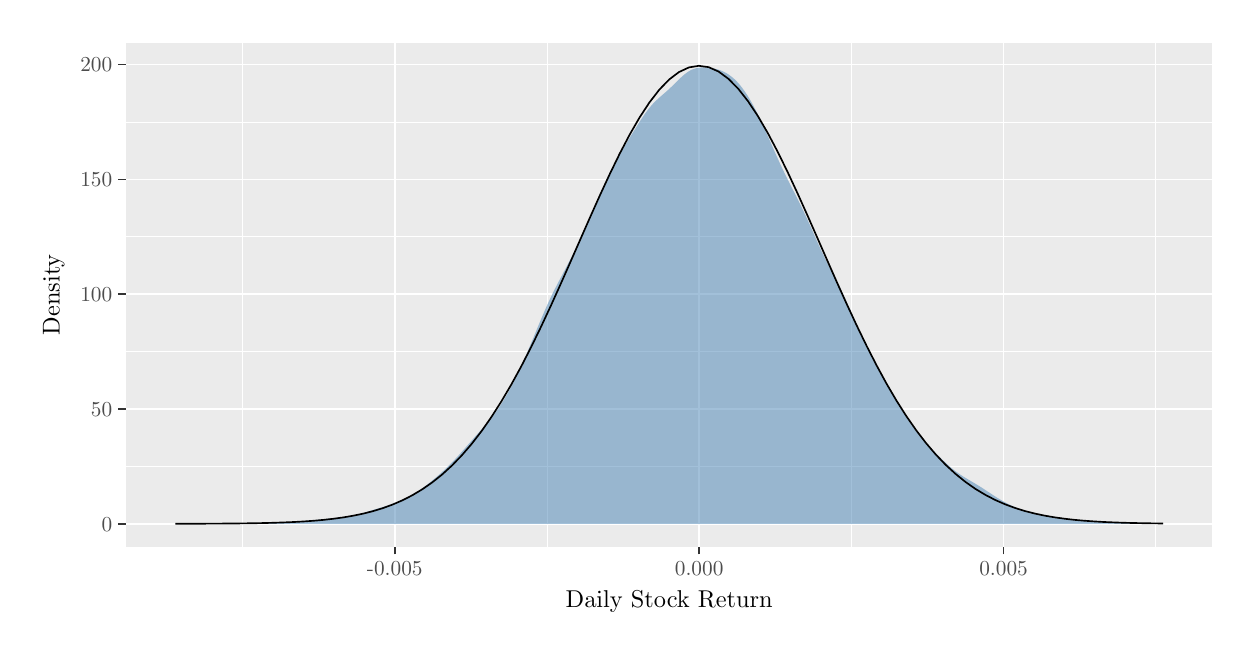
\begin{tikzpicture}[x=1pt,y=1pt]
\definecolor{fillColor}{RGB}{255,255,255}
\path[use as bounding box,fill=fillColor,fill opacity=0.00] (0,0) rectangle (433.62,216.81);
\begin{scope}
\path[clip] (  0.00,  0.00) rectangle (433.62,216.81);
\definecolor{drawColor}{RGB}{255,255,255}
\definecolor{fillColor}{RGB}{255,255,255}

\path[draw=drawColor,line width= 0.6pt,line join=round,line cap=round,fill=fillColor] (  0.00,  0.00) rectangle (433.62,216.81);
\end{scope}
\begin{scope}
\path[clip] ( 35.50, 29.26) rectangle (428.12,211.31);
\definecolor{fillColor}{gray}{0.92}

\path[fill=fillColor] ( 35.50, 29.26) rectangle (428.12,211.31);
\definecolor{drawColor}{RGB}{255,255,255}

\path[draw=drawColor,line width= 0.3pt,line join=round] ( 35.50, 58.28) --
	(428.12, 58.28);

\path[draw=drawColor,line width= 0.3pt,line join=round] ( 35.50, 99.76) --
	(428.12, 99.76);

\path[draw=drawColor,line width= 0.3pt,line join=round] ( 35.50,141.25) --
	(428.12,141.25);

\path[draw=drawColor,line width= 0.3pt,line join=round] ( 35.50,182.73) --
	(428.12,182.73);

\path[draw=drawColor,line width= 0.3pt,line join=round] ( 77.67, 29.26) --
	( 77.67,211.31);

\path[draw=drawColor,line width= 0.3pt,line join=round] (187.65, 29.26) --
	(187.65,211.31);

\path[draw=drawColor,line width= 0.3pt,line join=round] (297.64, 29.26) --
	(297.64,211.31);

\path[draw=drawColor,line width= 0.3pt,line join=round] (407.62, 29.26) --
	(407.62,211.31);

\path[draw=drawColor,line width= 0.6pt,line join=round] ( 35.50, 37.53) --
	(428.12, 37.53);

\path[draw=drawColor,line width= 0.6pt,line join=round] ( 35.50, 79.02) --
	(428.12, 79.02);

\path[draw=drawColor,line width= 0.6pt,line join=round] ( 35.50,120.50) --
	(428.12,120.50);

\path[draw=drawColor,line width= 0.6pt,line join=round] ( 35.50,161.99) --
	(428.12,161.99);

\path[draw=drawColor,line width= 0.6pt,line join=round] ( 35.50,203.47) --
	(428.12,203.47);

\path[draw=drawColor,line width= 0.6pt,line join=round] (132.66, 29.26) --
	(132.66,211.31);

\path[draw=drawColor,line width= 0.6pt,line join=round] (242.64, 29.26) --
	(242.64,211.31);

\path[draw=drawColor,line width= 0.6pt,line join=round] (352.63, 29.26) --
	(352.63,211.31);
\definecolor{fillColor}{RGB}{70,130,180}

\path[fill=fillColor,fill opacity=0.50] ( 53.35, 37.57) --
	( 54.05, 37.57) --
	( 54.75, 37.57) --
	( 55.44, 37.57) --
	( 56.14, 37.57) --
	( 56.84, 37.56) --
	( 57.54, 37.56) --
	( 58.24, 37.56) --
	( 58.94, 37.55) --
	( 59.63, 37.55) --
	( 60.33, 37.55) --
	( 61.03, 37.54) --
	( 61.73, 37.54) --
	( 62.43, 37.54) --
	( 63.13, 37.54) --
	( 63.83, 37.54) --
	( 64.52, 37.54) --
	( 65.22, 37.54) --
	( 65.92, 37.54) --
	( 66.62, 37.55) --
	( 67.32, 37.55) --
	( 68.02, 37.56) --
	( 68.71, 37.56) --
	( 69.41, 37.57) --
	( 70.11, 37.58) --
	( 70.81, 37.58) --
	( 71.51, 37.59) --
	( 72.21, 37.61) --
	( 72.91, 37.62) --
	( 73.60, 37.63) --
	( 74.30, 37.64) --
	( 75.00, 37.66) --
	( 75.70, 37.67) --
	( 76.40, 37.69) --
	( 77.10, 37.70) --
	( 77.80, 37.71) --
	( 78.49, 37.73) --
	( 79.19, 37.74) --
	( 79.89, 37.75) --
	( 80.59, 37.76) --
	( 81.29, 37.77) --
	( 81.99, 37.78) --
	( 82.68, 37.78) --
	( 83.38, 37.79) --
	( 84.08, 37.80) --
	( 84.78, 37.81) --
	( 85.48, 37.81) --
	( 86.18, 37.82) --
	( 86.88, 37.83) --
	( 87.57, 37.85) --
	( 88.27, 37.86) --
	( 88.97, 37.88) --
	( 89.67, 37.90) --
	( 90.37, 37.92) --
	( 91.07, 37.94) --
	( 91.76, 37.97) --
	( 92.46, 38.00) --
	( 93.16, 38.03) --
	( 93.86, 38.07) --
	( 94.56, 38.10) --
	( 95.26, 38.15) --
	( 95.96, 38.19) --
	( 96.65, 38.24) --
	( 97.35, 38.29) --
	( 98.05, 38.34) --
	( 98.75, 38.40) --
	( 99.45, 38.46) --
	(100.15, 38.52) --
	(100.85, 38.58) --
	(101.54, 38.64) --
	(102.24, 38.71) --
	(102.94, 38.77) --
	(103.64, 38.84) --
	(104.34, 38.91) --
	(105.04, 38.99) --
	(105.73, 39.06) --
	(106.43, 39.14) --
	(107.13, 39.22) --
	(107.83, 39.30) --
	(108.53, 39.38) --
	(109.23, 39.45) --
	(109.93, 39.53) --
	(110.62, 39.60) --
	(111.32, 39.67) --
	(112.02, 39.74) --
	(112.72, 39.81) --
	(113.42, 39.88) --
	(114.12, 39.95) --
	(114.81, 40.03) --
	(115.51, 40.12) --
	(116.21, 40.22) --
	(116.91, 40.33) --
	(117.61, 40.47) --
	(118.31, 40.61) --
	(119.01, 40.77) --
	(119.70, 40.95) --
	(120.40, 41.15) --
	(121.10, 41.35) --
	(121.80, 41.56) --
	(122.50, 41.78) --
	(123.20, 42.01) --
	(123.90, 42.23) --
	(124.59, 42.45) --
	(125.29, 42.67) --
	(125.99, 42.89) --
	(126.69, 43.10) --
	(127.39, 43.31) --
	(128.09, 43.51) --
	(128.78, 43.71) --
	(129.48, 43.92) --
	(130.18, 44.13) --
	(130.88, 44.35) --
	(131.58, 44.57) --
	(132.28, 44.81) --
	(132.98, 45.06) --
	(133.67, 45.33) --
	(134.37, 45.61) --
	(135.07, 45.91) --
	(135.77, 46.22) --
	(136.47, 46.56) --
	(137.17, 46.91) --
	(137.86, 47.29) --
	(138.56, 47.69) --
	(139.26, 48.11) --
	(139.96, 48.54) --
	(140.66, 49.00) --
	(141.36, 49.48) --
	(142.06, 49.97) --
	(142.75, 50.48) --
	(143.45, 51.00) --
	(144.15, 51.53) --
	(144.85, 52.08) --
	(145.55, 52.64) --
	(146.25, 53.21) --
	(146.95, 53.78) --
	(147.64, 54.37) --
	(148.34, 54.98) --
	(149.04, 55.59) --
	(149.74, 56.22) --
	(150.44, 56.86) --
	(151.14, 57.52) --
	(151.83, 58.20) --
	(152.53, 58.89) --
	(153.23, 59.60) --
	(153.93, 60.33) --
	(154.63, 61.08) --
	(155.33, 61.83) --
	(156.03, 62.60) --
	(156.72, 63.38) --
	(157.42, 64.17) --
	(158.12, 64.96) --
	(158.82, 65.76) --
	(159.52, 66.56) --
	(160.22, 67.36) --
	(160.91, 68.15) --
	(161.61, 68.95) --
	(162.31, 69.74) --
	(163.01, 70.52) --
	(163.71, 71.31) --
	(164.41, 72.10) --
	(165.11, 72.90) --
	(165.80, 73.70) --
	(166.50, 74.52) --
	(167.20, 75.37) --
	(167.90, 76.25) --
	(168.60, 77.16) --
	(169.30, 78.11) --
	(170.00, 79.10) --
	(170.69, 80.15) --
	(171.39, 81.24) --
	(172.09, 82.37) --
	(172.79, 83.56) --
	(173.49, 84.80) --
	(174.19, 86.09) --
	(174.88, 87.42) --
	(175.58, 88.80) --
	(176.28, 90.21) --
	(176.98, 91.66) --
	(177.68, 93.15) --
	(178.38, 94.66) --
	(179.08, 96.21) --
	(179.77, 97.79) --
	(180.47, 99.40) --
	(181.17,101.03) --
	(181.87,102.68) --
	(182.57,104.35) --
	(183.27,106.04) --
	(183.96,107.73) --
	(184.66,109.42) --
	(185.36,111.10) --
	(186.06,112.75) --
	(186.76,114.38) --
	(187.46,115.97) --
	(188.16,117.52) --
	(188.85,119.02) --
	(189.55,120.48) --
	(190.25,121.89) --
	(190.95,123.27) --
	(191.65,124.62) --
	(192.35,125.95) --
	(193.05,127.27) --
	(193.74,128.59) --
	(194.44,129.92) --
	(195.14,131.25) --
	(195.84,132.60) --
	(196.54,133.96) --
	(197.24,135.35) --
	(197.93,136.75) --
	(198.63,138.18) --
	(199.33,139.62) --
	(200.03,141.09) --
	(200.73,142.59) --
	(201.43,144.11) --
	(202.13,145.65) --
	(202.82,147.23) --
	(203.52,148.83) --
	(204.22,150.45) --
	(204.92,152.09) --
	(205.62,153.74) --
	(206.32,155.38) --
	(207.01,157.02) --
	(207.71,158.63) --
	(208.41,160.22) --
	(209.11,161.76) --
	(209.81,163.27) --
	(210.51,164.72) --
	(211.21,166.11) --
	(211.90,167.46) --
	(212.60,168.75) --
	(213.30,170.00) --
	(214.00,171.22) --
	(214.70,172.40) --
	(215.40,173.56) --
	(216.10,174.70) --
	(216.79,175.84) --
	(217.49,176.97) --
	(218.19,178.10) --
	(218.89,179.22) --
	(219.59,180.35) --
	(220.29,181.47) --
	(220.98,182.57) --
	(221.68,183.65) --
	(222.38,184.71) --
	(223.08,185.72) --
	(223.78,186.69) --
	(224.48,187.60) --
	(225.18,188.44) --
	(225.87,189.23) --
	(226.57,189.96) --
	(227.27,190.64) --
	(227.97,191.29) --
	(228.67,191.90) --
	(229.37,192.51) --
	(230.06,193.11) --
	(230.76,193.72) --
	(231.46,194.34) --
	(232.16,194.99) --
	(232.86,195.66) --
	(233.56,196.34) --
	(234.26,197.04) --
	(234.95,197.73) --
	(235.65,198.41) --
	(236.35,199.06) --
	(237.05,199.67) --
	(237.75,200.24) --
	(238.45,200.75) --
	(239.15,201.19) --
	(239.84,201.56) --
	(240.54,201.85) --
	(241.24,202.08) --
	(241.94,202.25) --
	(242.64,202.36) --
	(243.34,202.42) --
	(244.03,202.44) --
	(244.73,202.43) --
	(245.43,202.39) --
	(246.13,202.32) --
	(246.83,202.24) --
	(247.53,202.12) --
	(248.23,201.99) --
	(248.92,201.82) --
	(249.62,201.62) --
	(250.32,201.38) --
	(251.02,201.11) --
	(251.72,200.78) --
	(252.42,200.41) --
	(253.11,199.99) --
	(253.81,199.50) --
	(254.51,198.96) --
	(255.21,198.36) --
	(255.91,197.69) --
	(256.61,196.96) --
	(257.31,196.16) --
	(258.00,195.29) --
	(258.70,194.35) --
	(259.40,193.35) --
	(260.10,192.28) --
	(260.80,191.14) --
	(261.50,189.94) --
	(262.20,188.68) --
	(262.89,187.36) --
	(263.59,185.99) --
	(264.29,184.57) --
	(264.99,183.10) --
	(265.69,181.60) --
	(266.39,180.05) --
	(267.08,178.49) --
	(267.78,176.90) --
	(268.48,175.30) --
	(269.18,173.70) --
	(269.88,172.11) --
	(270.58,170.53) --
	(271.28,168.98) --
	(271.97,167.45) --
	(272.67,165.96) --
	(273.37,164.50) --
	(274.07,163.07) --
	(274.77,161.66) --
	(275.47,160.27) --
	(276.16,158.90) --
	(276.86,157.53) --
	(277.56,156.16) --
	(278.26,154.77) --
	(278.96,153.37) --
	(279.66,151.94) --
	(280.36,150.48) --
	(281.05,148.99) --
	(281.75,147.47) --
	(282.45,145.93) --
	(283.15,144.36) --
	(283.85,142.78) --
	(284.55,141.20) --
	(285.25,139.62) --
	(285.94,138.07) --
	(286.64,136.55) --
	(287.34,135.06) --
	(288.04,133.61) --
	(288.74,132.19) --
	(289.44,130.81) --
	(290.13,129.45) --
	(290.83,128.11) --
	(291.53,126.76) --
	(292.23,125.41) --
	(292.93,124.03) --
	(293.63,122.63) --
	(294.33,121.18) --
	(295.02,119.70) --
	(295.72,118.17) --
	(296.42,116.62) --
	(297.12,115.03) --
	(297.82,113.42) --
	(298.52,111.80) --
	(299.21,110.18) --
	(299.91,108.58) --
	(300.61,106.99) --
	(301.31,105.43) --
	(302.01,103.90) --
	(302.71,102.40) --
	(303.41,100.94) --
	(304.10, 99.52) --
	(304.80, 98.13) --
	(305.50, 96.78) --
	(306.20, 95.46) --
	(306.90, 94.17) --
	(307.60, 92.90) --
	(308.30, 91.65) --
	(308.99, 90.41) --
	(309.69, 89.19) --
	(310.39, 87.98) --
	(311.09, 86.78) --
	(311.79, 85.58) --
	(312.49, 84.39) --
	(313.18, 83.20) --
	(313.88, 82.01) --
	(314.58, 80.84) --
	(315.28, 79.67) --
	(315.98, 78.52) --
	(316.68, 77.38) --
	(317.38, 76.26) --
	(318.07, 75.18) --
	(318.77, 74.12) --
	(319.47, 73.10) --
	(320.17, 72.12) --
	(320.87, 71.18) --
	(321.57, 70.28) --
	(322.26, 69.41) --
	(322.96, 68.58) --
	(323.66, 67.78) --
	(324.36, 67.01) --
	(325.06, 66.25) --
	(325.76, 65.51) --
	(326.46, 64.79) --
	(327.15, 64.07) --
	(327.85, 63.36) --
	(328.55, 62.66) --
	(329.25, 61.96) --
	(329.95, 61.27) --
	(330.65, 60.58) --
	(331.35, 59.91) --
	(332.04, 59.26) --
	(332.74, 58.62) --
	(333.44, 58.01) --
	(334.14, 57.42) --
	(334.84, 56.86) --
	(335.54, 56.33) --
	(336.23, 55.83) --
	(336.93, 55.35) --
	(337.63, 54.89) --
	(338.33, 54.46) --
	(339.03, 54.03) --
	(339.73, 53.62) --
	(340.43, 53.21) --
	(341.12, 52.80) --
	(341.82, 52.39) --
	(342.52, 51.97) --
	(343.22, 51.55) --
	(343.92, 51.12) --
	(344.62, 50.68) --
	(345.31, 50.23) --
	(346.01, 49.77) --
	(346.71, 49.31) --
	(347.41, 48.85) --
	(348.11, 48.39) --
	(348.81, 47.93) --
	(349.51, 47.48) --
	(350.20, 47.04) --
	(350.90, 46.60) --
	(351.60, 46.18) --
	(352.30, 45.78) --
	(353.00, 45.38) --
	(353.70, 45.01) --
	(354.39, 44.65) --
	(355.09, 44.31) --
	(355.79, 43.98) --
	(356.49, 43.67) --
	(357.19, 43.37) --
	(357.89, 43.09) --
	(358.59, 42.82) --
	(359.28, 42.56) --
	(359.98, 42.32) --
	(360.68, 42.10) --
	(361.38, 41.88) --
	(362.08, 41.68) --
	(362.78, 41.50) --
	(363.48, 41.32) --
	(364.17, 41.16) --
	(364.87, 41.01) --
	(365.57, 40.86) --
	(366.27, 40.73) --
	(366.97, 40.60) --
	(367.67, 40.48) --
	(368.36, 40.36) --
	(369.06, 40.25) --
	(369.76, 40.15) --
	(370.46, 40.05) --
	(371.16, 39.95) --
	(371.86, 39.85) --
	(372.56, 39.76) --
	(373.25, 39.67) --
	(373.95, 39.58) --
	(374.65, 39.49) --
	(375.35, 39.40) --
	(376.05, 39.32) --
	(376.75, 39.23) --
	(377.44, 39.15) --
	(378.14, 39.06) --
	(378.84, 38.98) --
	(379.54, 38.90) --
	(380.24, 38.82) --
	(380.94, 38.74) --
	(381.64, 38.66) --
	(382.33, 38.59) --
	(383.03, 38.53) --
	(383.73, 38.46) --
	(384.43, 38.40) --
	(385.13, 38.35) --
	(385.83, 38.29) --
	(386.53, 38.25) --
	(387.22, 38.20) --
	(387.92, 38.16) --
	(388.62, 38.12) --
	(389.32, 38.08) --
	(390.02, 38.04) --
	(390.72, 38.01) --
	(391.41, 37.98) --
	(392.11, 37.95) --
	(392.81, 37.93) --
	(393.51, 37.90) --
	(394.21, 37.89) --
	(394.91, 37.87) --
	(395.61, 37.86) --
	(396.30, 37.85) --
	(397.00, 37.84) --
	(397.70, 37.84) --
	(398.40, 37.83) --
	(399.10, 37.83) --
	(399.80, 37.83) --
	(400.49, 37.83) --
	(401.19, 37.83) --
	(401.89, 37.83) --
	(402.59, 37.82) --
	(403.29, 37.82) --
	(403.99, 37.81) --
	(404.69, 37.80) --
	(405.38, 37.79) --
	(406.08, 37.78) --
	(406.78, 37.76) --
	(407.48, 37.75) --
	(408.18, 37.73) --
	(408.88, 37.72) --
	(409.58, 37.70) --
	(410.27, 37.69) --
	(410.27, 37.53) --
	(409.58, 37.53) --
	(408.88, 37.53) --
	(408.18, 37.53) --
	(407.48, 37.53) --
	(406.78, 37.53) --
	(406.08, 37.53) --
	(405.38, 37.53) --
	(404.69, 37.53) --
	(403.99, 37.53) --
	(403.29, 37.53) --
	(402.59, 37.53) --
	(401.89, 37.53) --
	(401.19, 37.53) --
	(400.49, 37.53) --
	(399.80, 37.53) --
	(399.10, 37.53) --
	(398.40, 37.53) --
	(397.70, 37.53) --
	(397.00, 37.53) --
	(396.30, 37.53) --
	(395.61, 37.53) --
	(394.91, 37.53) --
	(394.21, 37.53) --
	(393.51, 37.53) --
	(392.81, 37.53) --
	(392.11, 37.53) --
	(391.41, 37.53) --
	(390.72, 37.53) --
	(390.02, 37.53) --
	(389.32, 37.53) --
	(388.62, 37.53) --
	(387.92, 37.53) --
	(387.22, 37.53) --
	(386.53, 37.53) --
	(385.83, 37.53) --
	(385.13, 37.53) --
	(384.43, 37.53) --
	(383.73, 37.53) --
	(383.03, 37.53) --
	(382.33, 37.53) --
	(381.64, 37.53) --
	(380.94, 37.53) --
	(380.24, 37.53) --
	(379.54, 37.53) --
	(378.84, 37.53) --
	(378.14, 37.53) --
	(377.44, 37.53) --
	(376.75, 37.53) --
	(376.05, 37.53) --
	(375.35, 37.53) --
	(374.65, 37.53) --
	(373.95, 37.53) --
	(373.25, 37.53) --
	(372.56, 37.53) --
	(371.86, 37.53) --
	(371.16, 37.53) --
	(370.46, 37.53) --
	(369.76, 37.53) --
	(369.06, 37.53) --
	(368.36, 37.53) --
	(367.67, 37.53) --
	(366.97, 37.53) --
	(366.27, 37.53) --
	(365.57, 37.53) --
	(364.87, 37.53) --
	(364.17, 37.53) --
	(363.48, 37.53) --
	(362.78, 37.53) --
	(362.08, 37.53) --
	(361.38, 37.53) --
	(360.68, 37.53) --
	(359.98, 37.53) --
	(359.28, 37.53) --
	(358.59, 37.53) --
	(357.89, 37.53) --
	(357.19, 37.53) --
	(356.49, 37.53) --
	(355.79, 37.53) --
	(355.09, 37.53) --
	(354.39, 37.53) --
	(353.70, 37.53) --
	(353.00, 37.53) --
	(352.30, 37.53) --
	(351.60, 37.53) --
	(350.90, 37.53) --
	(350.20, 37.53) --
	(349.51, 37.53) --
	(348.81, 37.53) --
	(348.11, 37.53) --
	(347.41, 37.53) --
	(346.71, 37.53) --
	(346.01, 37.53) --
	(345.31, 37.53) --
	(344.62, 37.53) --
	(343.92, 37.53) --
	(343.22, 37.53) --
	(342.52, 37.53) --
	(341.82, 37.53) --
	(341.12, 37.53) --
	(340.43, 37.53) --
	(339.73, 37.53) --
	(339.03, 37.53) --
	(338.33, 37.53) --
	(337.63, 37.53) --
	(336.93, 37.53) --
	(336.23, 37.53) --
	(335.54, 37.53) --
	(334.84, 37.53) --
	(334.14, 37.53) --
	(333.44, 37.53) --
	(332.74, 37.53) --
	(332.04, 37.53) --
	(331.35, 37.53) --
	(330.65, 37.53) --
	(329.95, 37.53) --
	(329.25, 37.53) --
	(328.55, 37.53) --
	(327.85, 37.53) --
	(327.15, 37.53) --
	(326.46, 37.53) --
	(325.76, 37.53) --
	(325.06, 37.53) --
	(324.36, 37.53) --
	(323.66, 37.53) --
	(322.96, 37.53) --
	(322.26, 37.53) --
	(321.57, 37.53) --
	(320.87, 37.53) --
	(320.17, 37.53) --
	(319.47, 37.53) --
	(318.77, 37.53) --
	(318.07, 37.53) --
	(317.38, 37.53) --
	(316.68, 37.53) --
	(315.98, 37.53) --
	(315.28, 37.53) --
	(314.58, 37.53) --
	(313.88, 37.53) --
	(313.18, 37.53) --
	(312.49, 37.53) --
	(311.79, 37.53) --
	(311.09, 37.53) --
	(310.39, 37.53) --
	(309.69, 37.53) --
	(308.99, 37.53) --
	(308.30, 37.53) --
	(307.60, 37.53) --
	(306.90, 37.53) --
	(306.20, 37.53) --
	(305.50, 37.53) --
	(304.80, 37.53) --
	(304.10, 37.53) --
	(303.41, 37.53) --
	(302.71, 37.53) --
	(302.01, 37.53) --
	(301.31, 37.53) --
	(300.61, 37.53) --
	(299.91, 37.53) --
	(299.21, 37.53) --
	(298.52, 37.53) --
	(297.82, 37.53) --
	(297.12, 37.53) --
	(296.42, 37.53) --
	(295.72, 37.53) --
	(295.02, 37.53) --
	(294.33, 37.53) --
	(293.63, 37.53) --
	(292.93, 37.53) --
	(292.23, 37.53) --
	(291.53, 37.53) --
	(290.83, 37.53) --
	(290.13, 37.53) --
	(289.44, 37.53) --
	(288.74, 37.53) --
	(288.04, 37.53) --
	(287.34, 37.53) --
	(286.64, 37.53) --
	(285.94, 37.53) --
	(285.25, 37.53) --
	(284.55, 37.53) --
	(283.85, 37.53) --
	(283.15, 37.53) --
	(282.45, 37.53) --
	(281.75, 37.53) --
	(281.05, 37.53) --
	(280.36, 37.53) --
	(279.66, 37.53) --
	(278.96, 37.53) --
	(278.26, 37.53) --
	(277.56, 37.53) --
	(276.86, 37.53) --
	(276.16, 37.53) --
	(275.47, 37.53) --
	(274.77, 37.53) --
	(274.07, 37.53) --
	(273.37, 37.53) --
	(272.67, 37.53) --
	(271.97, 37.53) --
	(271.28, 37.53) --
	(270.58, 37.53) --
	(269.88, 37.53) --
	(269.18, 37.53) --
	(268.48, 37.53) --
	(267.78, 37.53) --
	(267.08, 37.53) --
	(266.39, 37.53) --
	(265.69, 37.53) --
	(264.99, 37.53) --
	(264.29, 37.53) --
	(263.59, 37.53) --
	(262.89, 37.53) --
	(262.20, 37.53) --
	(261.50, 37.53) --
	(260.80, 37.53) --
	(260.10, 37.53) --
	(259.40, 37.53) --
	(258.70, 37.53) --
	(258.00, 37.53) --
	(257.31, 37.53) --
	(256.61, 37.53) --
	(255.91, 37.53) --
	(255.21, 37.53) --
	(254.51, 37.53) --
	(253.81, 37.53) --
	(253.11, 37.53) --
	(252.42, 37.53) --
	(251.72, 37.53) --
	(251.02, 37.53) --
	(250.32, 37.53) --
	(249.62, 37.53) --
	(248.92, 37.53) --
	(248.23, 37.53) --
	(247.53, 37.53) --
	(246.83, 37.53) --
	(246.13, 37.53) --
	(245.43, 37.53) --
	(244.73, 37.53) --
	(244.03, 37.53) --
	(243.34, 37.53) --
	(242.64, 37.53) --
	(241.94, 37.53) --
	(241.24, 37.53) --
	(240.54, 37.53) --
	(239.84, 37.53) --
	(239.15, 37.53) --
	(238.45, 37.53) --
	(237.75, 37.53) --
	(237.05, 37.53) --
	(236.35, 37.53) --
	(235.65, 37.53) --
	(234.95, 37.53) --
	(234.26, 37.53) --
	(233.56, 37.53) --
	(232.86, 37.53) --
	(232.16, 37.53) --
	(231.46, 37.53) --
	(230.76, 37.53) --
	(230.06, 37.53) --
	(229.37, 37.53) --
	(228.67, 37.53) --
	(227.97, 37.53) --
	(227.27, 37.53) --
	(226.57, 37.53) --
	(225.87, 37.53) --
	(225.18, 37.53) --
	(224.48, 37.53) --
	(223.78, 37.53) --
	(223.08, 37.53) --
	(222.38, 37.53) --
	(221.68, 37.53) --
	(220.98, 37.53) --
	(220.29, 37.53) --
	(219.59, 37.53) --
	(218.89, 37.53) --
	(218.19, 37.53) --
	(217.49, 37.53) --
	(216.79, 37.53) --
	(216.10, 37.53) --
	(215.40, 37.53) --
	(214.70, 37.53) --
	(214.00, 37.53) --
	(213.30, 37.53) --
	(212.60, 37.53) --
	(211.90, 37.53) --
	(211.21, 37.53) --
	(210.51, 37.53) --
	(209.81, 37.53) --
	(209.11, 37.53) --
	(208.41, 37.53) --
	(207.71, 37.53) --
	(207.01, 37.53) --
	(206.32, 37.53) --
	(205.62, 37.53) --
	(204.92, 37.53) --
	(204.22, 37.53) --
	(203.52, 37.53) --
	(202.82, 37.53) --
	(202.13, 37.53) --
	(201.43, 37.53) --
	(200.73, 37.53) --
	(200.03, 37.53) --
	(199.33, 37.53) --
	(198.63, 37.53) --
	(197.93, 37.53) --
	(197.24, 37.53) --
	(196.54, 37.53) --
	(195.84, 37.53) --
	(195.14, 37.53) --
	(194.44, 37.53) --
	(193.74, 37.53) --
	(193.05, 37.53) --
	(192.35, 37.53) --
	(191.65, 37.53) --
	(190.95, 37.53) --
	(190.25, 37.53) --
	(189.55, 37.53) --
	(188.85, 37.53) --
	(188.16, 37.53) --
	(187.46, 37.53) --
	(186.76, 37.53) --
	(186.06, 37.53) --
	(185.36, 37.53) --
	(184.66, 37.53) --
	(183.96, 37.53) --
	(183.27, 37.53) --
	(182.57, 37.53) --
	(181.87, 37.53) --
	(181.17, 37.53) --
	(180.47, 37.53) --
	(179.77, 37.53) --
	(179.08, 37.53) --
	(178.38, 37.53) --
	(177.68, 37.53) --
	(176.98, 37.53) --
	(176.28, 37.53) --
	(175.58, 37.53) --
	(174.88, 37.53) --
	(174.19, 37.53) --
	(173.49, 37.53) --
	(172.79, 37.53) --
	(172.09, 37.53) --
	(171.39, 37.53) --
	(170.69, 37.53) --
	(170.00, 37.53) --
	(169.30, 37.53) --
	(168.60, 37.53) --
	(167.90, 37.53) --
	(167.20, 37.53) --
	(166.50, 37.53) --
	(165.80, 37.53) --
	(165.11, 37.53) --
	(164.41, 37.53) --
	(163.71, 37.53) --
	(163.01, 37.53) --
	(162.31, 37.53) --
	(161.61, 37.53) --
	(160.91, 37.53) --
	(160.22, 37.53) --
	(159.52, 37.53) --
	(158.82, 37.53) --
	(158.12, 37.53) --
	(157.42, 37.53) --
	(156.72, 37.53) --
	(156.03, 37.53) --
	(155.33, 37.53) --
	(154.63, 37.53) --
	(153.93, 37.53) --
	(153.23, 37.53) --
	(152.53, 37.53) --
	(151.83, 37.53) --
	(151.14, 37.53) --
	(150.44, 37.53) --
	(149.74, 37.53) --
	(149.04, 37.53) --
	(148.34, 37.53) --
	(147.64, 37.53) --
	(146.95, 37.53) --
	(146.25, 37.53) --
	(145.55, 37.53) --
	(144.85, 37.53) --
	(144.15, 37.53) --
	(143.45, 37.53) --
	(142.75, 37.53) --
	(142.06, 37.53) --
	(141.36, 37.53) --
	(140.66, 37.53) --
	(139.96, 37.53) --
	(139.26, 37.53) --
	(138.56, 37.53) --
	(137.86, 37.53) --
	(137.17, 37.53) --
	(136.47, 37.53) --
	(135.77, 37.53) --
	(135.07, 37.53) --
	(134.37, 37.53) --
	(133.67, 37.53) --
	(132.98, 37.53) --
	(132.28, 37.53) --
	(131.58, 37.53) --
	(130.88, 37.53) --
	(130.18, 37.53) --
	(129.48, 37.53) --
	(128.78, 37.53) --
	(128.09, 37.53) --
	(127.39, 37.53) --
	(126.69, 37.53) --
	(125.99, 37.53) --
	(125.29, 37.53) --
	(124.59, 37.53) --
	(123.90, 37.53) --
	(123.20, 37.53) --
	(122.50, 37.53) --
	(121.80, 37.53) --
	(121.10, 37.53) --
	(120.40, 37.53) --
	(119.70, 37.53) --
	(119.01, 37.53) --
	(118.31, 37.53) --
	(117.61, 37.53) --
	(116.91, 37.53) --
	(116.21, 37.53) --
	(115.51, 37.53) --
	(114.81, 37.53) --
	(114.12, 37.53) --
	(113.42, 37.53) --
	(112.72, 37.53) --
	(112.02, 37.53) --
	(111.32, 37.53) --
	(110.62, 37.53) --
	(109.93, 37.53) --
	(109.23, 37.53) --
	(108.53, 37.53) --
	(107.83, 37.53) --
	(107.13, 37.53) --
	(106.43, 37.53) --
	(105.73, 37.53) --
	(105.04, 37.53) --
	(104.34, 37.53) --
	(103.64, 37.53) --
	(102.94, 37.53) --
	(102.24, 37.53) --
	(101.54, 37.53) --
	(100.85, 37.53) --
	(100.15, 37.53) --
	( 99.45, 37.53) --
	( 98.75, 37.53) --
	( 98.05, 37.53) --
	( 97.35, 37.53) --
	( 96.65, 37.53) --
	( 95.96, 37.53) --
	( 95.26, 37.53) --
	( 94.56, 37.53) --
	( 93.86, 37.53) --
	( 93.16, 37.53) --
	( 92.46, 37.53) --
	( 91.76, 37.53) --
	( 91.07, 37.53) --
	( 90.37, 37.53) --
	( 89.67, 37.53) --
	( 88.97, 37.53) --
	( 88.27, 37.53) --
	( 87.57, 37.53) --
	( 86.88, 37.53) --
	( 86.18, 37.53) --
	( 85.48, 37.53) --
	( 84.78, 37.53) --
	( 84.08, 37.53) --
	( 83.38, 37.53) --
	( 82.68, 37.53) --
	( 81.99, 37.53) --
	( 81.29, 37.53) --
	( 80.59, 37.53) --
	( 79.89, 37.53) --
	( 79.19, 37.53) --
	( 78.49, 37.53) --
	( 77.80, 37.53) --
	( 77.10, 37.53) --
	( 76.40, 37.53) --
	( 75.70, 37.53) --
	( 75.00, 37.53) --
	( 74.30, 37.53) --
	( 73.60, 37.53) --
	( 72.91, 37.53) --
	( 72.21, 37.53) --
	( 71.51, 37.53) --
	( 70.81, 37.53) --
	( 70.11, 37.53) --
	( 69.41, 37.53) --
	( 68.71, 37.53) --
	( 68.02, 37.53) --
	( 67.32, 37.53) --
	( 66.62, 37.53) --
	( 65.92, 37.53) --
	( 65.22, 37.53) --
	( 64.52, 37.53) --
	( 63.83, 37.53) --
	( 63.13, 37.53) --
	( 62.43, 37.53) --
	( 61.73, 37.53) --
	( 61.03, 37.53) --
	( 60.33, 37.53) --
	( 59.63, 37.53) --
	( 58.94, 37.53) --
	( 58.24, 37.53) --
	( 57.54, 37.53) --
	( 56.84, 37.53) --
	( 56.14, 37.53) --
	( 55.44, 37.53) --
	( 54.75, 37.53) --
	( 54.05, 37.53) --
	( 53.35, 37.53) --
	cycle;
\definecolor{drawColor}{RGB}{0,0,0}

\path[draw=drawColor,line width= 0.6pt,line join=round] ( 53.35, 37.55) --
	( 56.92, 37.56) --
	( 60.49, 37.56) --
	( 64.06, 37.58) --
	( 67.63, 37.59) --
	( 71.19, 37.62) --
	( 74.76, 37.65) --
	( 78.33, 37.69) --
	( 81.90, 37.74) --
	( 85.47, 37.81) --
	( 89.04, 37.91) --
	( 92.61, 38.03) --
	( 96.18, 38.18) --
	( 99.75, 38.38) --
	(103.32, 38.63) --
	(106.89, 38.95) --
	(110.46, 39.35) --
	(114.03, 39.84) --
	(117.59, 40.45) --
	(121.16, 41.19) --
	(124.73, 42.09) --
	(128.30, 43.18) --
	(131.87, 44.49) --
	(135.44, 46.03) --
	(139.01, 47.86) --
	(142.58, 49.99) --
	(146.15, 52.47) --
	(149.72, 55.31) --
	(153.29, 58.57) --
	(156.86, 62.26) --
	(160.43, 66.40) --
	(164.00, 71.01) --
	(167.56, 76.11) --
	(171.13, 81.70) --
	(174.70, 87.76) --
	(178.27, 94.27) --
	(181.84,101.22) --
	(185.41,108.54) --
	(188.98,116.18) --
	(192.55,124.08) --
	(196.12,132.14) --
	(199.69,140.28) --
	(203.26,148.39) --
	(206.83,156.35) --
	(210.40,164.04) --
	(213.96,171.35) --
	(217.53,178.16) --
	(221.10,184.34) --
	(224.67,189.79) --
	(228.24,194.40) --
	(231.81,198.09) --
	(235.38,200.79) --
	(238.95,202.45) --
	(242.52,203.03) --
	(246.09,202.53) --
	(249.66,200.95) --
	(253.23,198.32) --
	(256.80,194.69) --
	(260.37,190.14) --
	(263.93,184.75) --
	(267.50,178.62) --
	(271.07,171.85) --
	(274.64,164.57) --
	(278.21,156.90) --
	(281.78,148.95) --
	(285.35,140.86) --
	(288.92,132.72) --
	(292.49,124.64) --
	(296.06,116.73) --
	(299.63,109.07) --
	(303.20,101.72) --
	(306.77, 94.75) --
	(310.33, 88.20) --
	(313.90, 82.11) --
	(317.47, 76.49) --
	(321.04, 71.36) --
	(324.61, 66.71) --
	(328.18, 62.53) --
	(331.75, 58.81) --
	(335.32, 55.53) --
	(338.89, 52.65) --
	(342.46, 50.15) --
	(346.03, 48.00) --
	(349.60, 46.15) --
	(353.17, 44.59) --
	(356.73, 43.27) --
	(360.30, 42.16) --
	(363.87, 41.25) --
	(367.44, 40.49) --
	(371.01, 39.88) --
	(374.58, 39.38) --
	(378.15, 38.97) --
	(381.72, 38.65) --
	(385.29, 38.40) --
	(388.86, 38.19) --
	(392.43, 38.04) --
	(396.00, 37.91) --
	(399.57, 37.82) --
	(403.14, 37.75) --
	(406.70, 37.69) --
	(410.27, 37.65);
\end{scope}
\begin{scope}
\path[clip] (  0.00,  0.00) rectangle (433.62,216.81);
\definecolor{drawColor}{gray}{0.30}

\node[text=drawColor,anchor=base east,inner sep=0pt, outer sep=0pt, scale=  0.77] at ( 30.55, 34.88) {0};

\node[text=drawColor,anchor=base east,inner sep=0pt, outer sep=0pt, scale=  0.77] at ( 30.55, 76.37) {50};

\node[text=drawColor,anchor=base east,inner sep=0pt, outer sep=0pt, scale=  0.77] at ( 30.55,117.85) {100};

\node[text=drawColor,anchor=base east,inner sep=0pt, outer sep=0pt, scale=  0.77] at ( 30.55,159.34) {150};

\node[text=drawColor,anchor=base east,inner sep=0pt, outer sep=0pt, scale=  0.77] at ( 30.55,200.82) {200};
\end{scope}
\begin{scope}
\path[clip] (  0.00,  0.00) rectangle (433.62,216.81);
\definecolor{drawColor}{gray}{0.20}

\path[draw=drawColor,line width= 0.6pt,line join=round] ( 32.75, 37.53) --
	( 35.50, 37.53);

\path[draw=drawColor,line width= 0.6pt,line join=round] ( 32.75, 79.02) --
	( 35.50, 79.02);

\path[draw=drawColor,line width= 0.6pt,line join=round] ( 32.75,120.50) --
	( 35.50,120.50);

\path[draw=drawColor,line width= 0.6pt,line join=round] ( 32.75,161.99) --
	( 35.50,161.99);

\path[draw=drawColor,line width= 0.6pt,line join=round] ( 32.75,203.47) --
	( 35.50,203.47);
\end{scope}
\begin{scope}
\path[clip] (  0.00,  0.00) rectangle (433.62,216.81);
\definecolor{drawColor}{gray}{0.20}

\path[draw=drawColor,line width= 0.6pt,line join=round] (132.66, 26.51) --
	(132.66, 29.26);

\path[draw=drawColor,line width= 0.6pt,line join=round] (242.64, 26.51) --
	(242.64, 29.26);

\path[draw=drawColor,line width= 0.6pt,line join=round] (352.63, 26.51) --
	(352.63, 29.26);
\end{scope}
\begin{scope}
\path[clip] (  0.00,  0.00) rectangle (433.62,216.81);
\definecolor{drawColor}{gray}{0.30}

\node[text=drawColor,anchor=base,inner sep=0pt, outer sep=0pt, scale=  0.77] at (132.66, 19.00) {-0.005};

\node[text=drawColor,anchor=base,inner sep=0pt, outer sep=0pt, scale=  0.77] at (242.64, 19.00) {0.000};

\node[text=drawColor,anchor=base,inner sep=0pt, outer sep=0pt, scale=  0.77] at (352.63, 19.00) {0.005};
\end{scope}
\begin{scope}
\path[clip] (  0.00,  0.00) rectangle (433.62,216.81);
\definecolor{drawColor}{RGB}{0,0,0}

\node[text=drawColor,anchor=base,inner sep=0pt, outer sep=0pt, scale=  0.88] at (231.81,  7.44) {Daily Stock Return};
\end{scope}
\begin{scope}
\path[clip] (  0.00,  0.00) rectangle (433.62,216.81);
\definecolor{drawColor}{RGB}{0,0,0}

\node[text=drawColor,rotate= 90.00,anchor=base,inner sep=0pt, outer sep=0pt, scale=  0.88] at ( 11.56,120.28) {Density};
\end{scope}
\end{tikzpicture}

\caption{Daily Basis Stock Return Density}
\label{p:returndensity}
\floatfoot{
The above density function has been constructed over 10000 samples of a unique process. The samples has been constructed following \cref{eq:Scontinuousdiffrate}. The arguments are set with the following value, $\alpha = 0$, $\sigma = 30\%$. The black density belongs to the normal bell curve with mean $\alpha$ and standard deviation of $\sigma \times \sqrt{dt}$. The period between each measure, namely $dt$ has been set to $10000^{-1}$. 
}
\end{figure}


%%%%%%%%%%%%%%%%%%%%%%%%%
%  Log-return
%%%%%%%%%%%%%%%%%%%%%%%%%

According to \cref{eq:underlyinglogreturn}, The distribution of the natural logarithm of the stock price return recorded over a time period of $t$ is characterized by \cref{eq:logreturndist}

\begin{center}
\begin{equation}
\ln{\frac{\St}{S\left(0\right)}} 
  \sim N((\alpha - \frac{\sigma^2}{2}) t, \sigma^2 t)
\label{eq:logreturndist}
\end{equation}
\end{center}  

\begin{figure}[!h]
\centering
% Created by tikzDevice version 0.11 on 2018-04-13 09:41:17
% !TEX encoding = UTF-8 Unicode
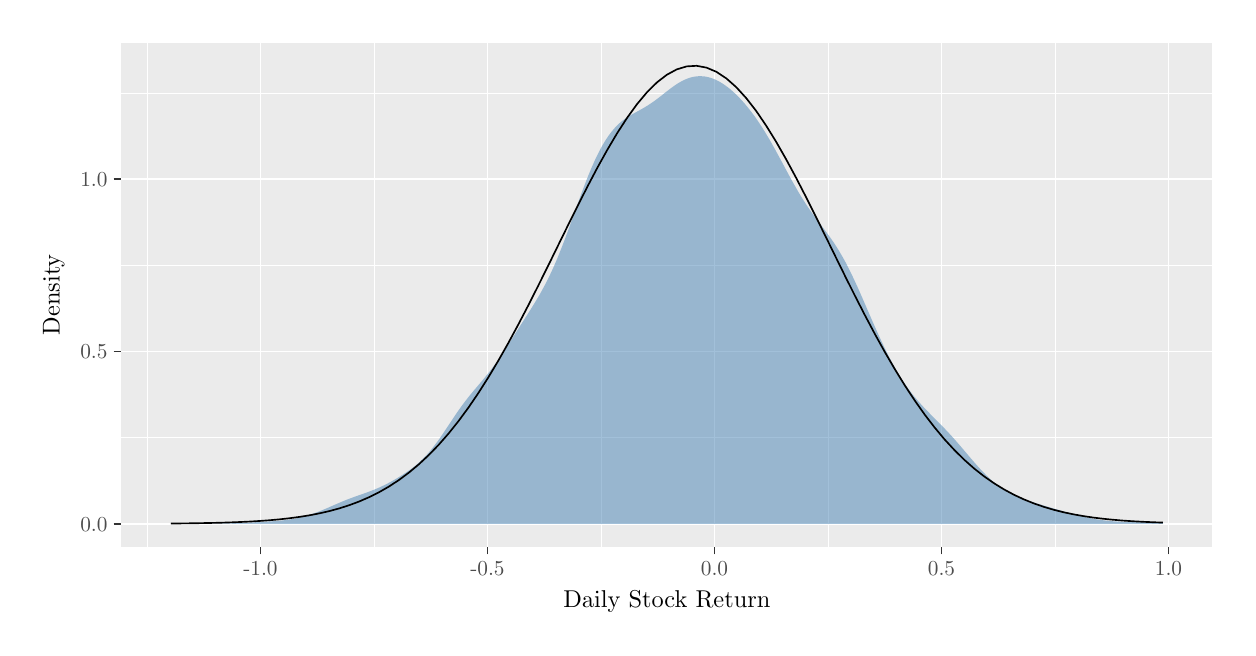
\begin{tikzpicture}[x=1pt,y=1pt]
\definecolor{fillColor}{RGB}{255,255,255}
\path[use as bounding box,fill=fillColor,fill opacity=0.00] (0,0) rectangle (433.62,216.81);
\begin{scope}
\path[clip] (  0.00,  0.00) rectangle (433.62,216.81);
\definecolor{drawColor}{RGB}{255,255,255}
\definecolor{fillColor}{RGB}{255,255,255}

\path[draw=drawColor,line width= 0.6pt,line join=round,line cap=round,fill=fillColor] (  0.00,  0.00) rectangle (433.62,216.81);
\end{scope}
\begin{scope}
\path[clip] ( 33.79, 29.26) rectangle (428.12,211.31);
\definecolor{fillColor}{gray}{0.92}

\path[fill=fillColor] ( 33.79, 29.26) rectangle (428.12,211.31);
\definecolor{drawColor}{RGB}{255,255,255}

\path[draw=drawColor,line width= 0.3pt,line join=round] ( 33.79, 68.65) --
	(428.12, 68.65);

\path[draw=drawColor,line width= 0.3pt,line join=round] ( 33.79,130.89) --
	(428.12,130.89);

\path[draw=drawColor,line width= 0.3pt,line join=round] ( 33.79,193.13) --
	(428.12,193.13);

\path[draw=drawColor,line width= 0.3pt,line join=round] ( 43.10, 29.26) --
	( 43.10,211.31);

\path[draw=drawColor,line width= 0.3pt,line join=round] (125.13, 29.26) --
	(125.13,211.31);

\path[draw=drawColor,line width= 0.3pt,line join=round] (207.16, 29.26) --
	(207.16,211.31);

\path[draw=drawColor,line width= 0.3pt,line join=round] (289.19, 29.26) --
	(289.19,211.31);

\path[draw=drawColor,line width= 0.3pt,line join=round] (371.23, 29.26) --
	(371.23,211.31);

\path[draw=drawColor,line width= 0.6pt,line join=round] ( 33.79, 37.53) --
	(428.12, 37.53);

\path[draw=drawColor,line width= 0.6pt,line join=round] ( 33.79, 99.77) --
	(428.12, 99.77);

\path[draw=drawColor,line width= 0.6pt,line join=round] ( 33.79,162.01) --
	(428.12,162.01);

\path[draw=drawColor,line width= 0.6pt,line join=round] ( 84.11, 29.26) --
	( 84.11,211.31);

\path[draw=drawColor,line width= 0.6pt,line join=round] (166.15, 29.26) --
	(166.15,211.31);

\path[draw=drawColor,line width= 0.6pt,line join=round] (248.18, 29.26) --
	(248.18,211.31);

\path[draw=drawColor,line width= 0.6pt,line join=round] (330.21, 29.26) --
	(330.21,211.31);

\path[draw=drawColor,line width= 0.6pt,line join=round] (412.24, 29.26) --
	(412.24,211.31);
\definecolor{fillColor}{RGB}{70,130,180}

\path[fill=fillColor,fill opacity=0.50] ( 51.72, 37.73) --
	( 52.42, 37.73) --
	( 53.12, 37.73) --
	( 53.82, 37.73) --
	( 54.52, 37.72) --
	( 55.22, 37.72) --
	( 55.92, 37.71) --
	( 56.63, 37.70) --
	( 57.33, 37.69) --
	( 58.03, 37.68) --
	( 58.73, 37.67) --
	( 59.43, 37.67) --
	( 60.13, 37.66) --
	( 60.84, 37.65) --
	( 61.54, 37.64) --
	( 62.24, 37.63) --
	( 62.94, 37.62) --
	( 63.64, 37.62) --
	( 64.34, 37.61) --
	( 65.04, 37.61) --
	( 65.75, 37.61) --
	( 66.45, 37.61) --
	( 67.15, 37.61) --
	( 67.85, 37.62) --
	( 68.55, 37.62) --
	( 69.25, 37.63) --
	( 69.96, 37.64) --
	( 70.66, 37.65) --
	( 71.36, 37.67) --
	( 72.06, 37.68) --
	( 72.76, 37.70) --
	( 73.46, 37.72) --
	( 74.16, 37.74) --
	( 74.87, 37.77) --
	( 75.57, 37.79) --
	( 76.27, 37.82) --
	( 76.97, 37.85) --
	( 77.67, 37.88) --
	( 78.37, 37.91) --
	( 79.07, 37.94) --
	( 79.78, 37.98) --
	( 80.48, 38.01) --
	( 81.18, 38.05) --
	( 81.88, 38.08) --
	( 82.58, 38.12) --
	( 83.28, 38.15) --
	( 83.99, 38.19) --
	( 84.69, 38.23) --
	( 85.39, 38.27) --
	( 86.09, 38.31) --
	( 86.79, 38.35) --
	( 87.49, 38.39) --
	( 88.19, 38.43) --
	( 88.90, 38.48) --
	( 89.60, 38.54) --
	( 90.30, 38.59) --
	( 91.00, 38.66) --
	( 91.70, 38.72) --
	( 92.40, 38.80) --
	( 93.11, 38.88) --
	( 93.81, 38.97) --
	( 94.51, 39.07) --
	( 95.21, 39.18) --
	( 95.91, 39.30) --
	( 96.61, 39.43) --
	( 97.31, 39.57) --
	( 98.02, 39.72) --
	( 98.72, 39.89) --
	( 99.42, 40.06) --
	(100.12, 40.25) --
	(100.82, 40.45) --
	(101.52, 40.67) --
	(102.23, 40.89) --
	(102.93, 41.13) --
	(103.63, 41.37) --
	(104.33, 41.63) --
	(105.03, 41.90) --
	(105.73, 42.18) --
	(106.43, 42.46) --
	(107.14, 42.75) --
	(107.84, 43.05) --
	(108.54, 43.35) --
	(109.24, 43.66) --
	(109.94, 43.96) --
	(110.64, 44.27) --
	(111.35, 44.58) --
	(112.05, 44.88) --
	(112.75, 45.18) --
	(113.45, 45.48) --
	(114.15, 45.77) --
	(114.85, 46.05) --
	(115.55, 46.33) --
	(116.26, 46.60) --
	(116.96, 46.86) --
	(117.66, 47.12) --
	(118.36, 47.37) --
	(119.06, 47.62) --
	(119.76, 47.87) --
	(120.47, 48.11) --
	(121.17, 48.36) --
	(121.87, 48.61) --
	(122.57, 48.86) --
	(123.27, 49.12) --
	(123.97, 49.38) --
	(124.67, 49.65) --
	(125.38, 49.93) --
	(126.08, 50.23) --
	(126.78, 50.53) --
	(127.48, 50.85) --
	(128.18, 51.18) --
	(128.88, 51.52) --
	(129.58, 51.87) --
	(130.29, 52.23) --
	(130.99, 52.60) --
	(131.69, 52.99) --
	(132.39, 53.38) --
	(133.09, 53.79) --
	(133.79, 54.20) --
	(134.50, 54.63) --
	(135.20, 55.07) --
	(135.90, 55.52) --
	(136.60, 55.98) --
	(137.30, 56.46) --
	(138.00, 56.95) --
	(138.70, 57.47) --
	(139.41, 58.00) --
	(140.11, 58.57) --
	(140.81, 59.16) --
	(141.51, 59.77) --
	(142.21, 60.42) --
	(142.91, 61.10) --
	(143.62, 61.82) --
	(144.32, 62.58) --
	(145.02, 63.38) --
	(145.72, 64.21) --
	(146.42, 65.09) --
	(147.12, 65.99) --
	(147.82, 66.93) --
	(148.53, 67.90) --
	(149.23, 68.91) --
	(149.93, 69.93) --
	(150.63, 70.97) --
	(151.33, 72.02) --
	(152.03, 73.08) --
	(152.74, 74.14) --
	(153.44, 75.20) --
	(154.14, 76.25) --
	(154.84, 77.29) --
	(155.54, 78.30) --
	(156.24, 79.30) --
	(156.94, 80.27) --
	(157.65, 81.22) --
	(158.35, 82.14) --
	(159.05, 83.04) --
	(159.75, 83.92) --
	(160.45, 84.78) --
	(161.15, 85.62) --
	(161.86, 86.45) --
	(162.56, 87.27) --
	(163.26, 88.10) --
	(163.96, 88.92) --
	(164.66, 89.76) --
	(165.36, 90.61) --
	(166.06, 91.47) --
	(166.77, 92.36) --
	(167.47, 93.27) --
	(168.17, 94.21) --
	(168.87, 95.17) --
	(169.57, 96.16) --
	(170.27, 97.16) --
	(170.98, 98.20) --
	(171.68, 99.25) --
	(172.38,100.32) --
	(173.08,101.40) --
	(173.78,102.50) --
	(174.48,103.60) --
	(175.18,104.70) --
	(175.89,105.81) --
	(176.59,106.91) --
	(177.29,108.01) --
	(177.99,109.11) --
	(178.69,110.21) --
	(179.39,111.31) --
	(180.09,112.40) --
	(180.80,113.50) --
	(181.50,114.61) --
	(182.20,115.72) --
	(182.90,116.86) --
	(183.60,118.01) --
	(184.30,119.18) --
	(185.01,120.38) --
	(185.71,121.63) --
	(186.41,122.91) --
	(187.11,124.24) --
	(187.81,125.61) --
	(188.51,127.03) --
	(189.21,128.51) --
	(189.92,130.05) --
	(190.62,131.65) --
	(191.32,133.30) --
	(192.02,135.01) --
	(192.72,136.76) --
	(193.42,138.57) --
	(194.13,140.41) --
	(194.83,142.30) --
	(195.53,144.22) --
	(196.23,146.16) --
	(196.93,148.12) --
	(197.63,150.08) --
	(198.33,152.04) --
	(199.04,153.99) --
	(199.74,155.92) --
	(200.44,157.82) --
	(201.14,159.68) --
	(201.84,161.50) --
	(202.54,163.27) --
	(203.25,164.99) --
	(203.95,166.64) --
	(204.65,168.22) --
	(205.35,169.74) --
	(206.05,171.18) --
	(206.75,172.55) --
	(207.45,173.85) --
	(208.16,175.07) --
	(208.86,176.20) --
	(209.56,177.27) --
	(210.26,178.26) --
	(210.96,179.18) --
	(211.66,180.03) --
	(212.37,180.82) --
	(213.07,181.54) --
	(213.77,182.20) --
	(214.47,182.81) --
	(215.17,183.37) --
	(215.87,183.89) --
	(216.57,184.37) --
	(217.28,184.82) --
	(217.98,185.24) --
	(218.68,185.64) --
	(219.38,186.03) --
	(220.08,186.42) --
	(220.78,186.80) --
	(221.49,187.19) --
	(222.19,187.58) --
	(222.89,187.99) --
	(223.59,188.41) --
	(224.29,188.85) --
	(224.99,189.31) --
	(225.69,189.78) --
	(226.40,190.28) --
	(227.10,190.79) --
	(227.80,191.32) --
	(228.50,191.86) --
	(229.20,192.41) --
	(229.90,192.97) --
	(230.60,193.52) --
	(231.31,194.07) --
	(232.01,194.61) --
	(232.71,195.13) --
	(233.41,195.64) --
	(234.11,196.12) --
	(234.81,196.58) --
	(235.52,197.01) --
	(236.22,197.41) --
	(236.92,197.77) --
	(237.62,198.09) --
	(238.32,198.38) --
	(239.02,198.63) --
	(239.72,198.84) --
	(240.43,199.01) --
	(241.13,199.14) --
	(241.83,199.22) --
	(242.53,199.27) --
	(243.23,199.27) --
	(243.93,199.24) --
	(244.64,199.17) --
	(245.34,199.05) --
	(246.04,198.89) --
	(246.74,198.69) --
	(247.44,198.45) --
	(248.14,198.18) --
	(248.84,197.87) --
	(249.55,197.52) --
	(250.25,197.13) --
	(250.95,196.70) --
	(251.65,196.24) --
	(252.35,195.74) --
	(253.05,195.22) --
	(253.76,194.66) --
	(254.46,194.06) --
	(255.16,193.43) --
	(255.86,192.77) --
	(256.56,192.08) --
	(257.26,191.36) --
	(257.96,190.61) --
	(258.67,189.83) --
	(259.37,189.02) --
	(260.07,188.18) --
	(260.77,187.30) --
	(261.47,186.40) --
	(262.17,185.47) --
	(262.88,184.50) --
	(263.58,183.50) --
	(264.28,182.47) --
	(264.98,181.40) --
	(265.68,180.31) --
	(266.38,179.18) --
	(267.08,178.02) --
	(267.79,176.84) --
	(268.49,175.62) --
	(269.19,174.39) --
	(269.89,173.13) --
	(270.59,171.85) --
	(271.29,170.56) --
	(272.00,169.26) --
	(272.70,167.95) --
	(273.40,166.64) --
	(274.10,165.33) --
	(274.80,164.03) --
	(275.50,162.74) --
	(276.20,161.46) --
	(276.91,160.21) --
	(277.61,158.98) --
	(278.31,157.77) --
	(279.01,156.59) --
	(279.71,155.44) --
	(280.41,154.32) --
	(281.11,153.23) --
	(281.82,152.17) --
	(282.52,151.15) --
	(283.22,150.14) --
	(283.92,149.16) --
	(284.62,148.20) --
	(285.32,147.26) --
	(286.03,146.32) --
	(286.73,145.40) --
	(287.43,144.47) --
	(288.13,143.54) --
	(288.83,142.59) --
	(289.53,141.63) --
	(290.23,140.65) --
	(290.94,139.64) --
	(291.64,138.59) --
	(292.34,137.50) --
	(293.04,136.38) --
	(293.74,135.21) --
	(294.44,134.00) --
	(295.15,132.74) --
	(295.85,131.42) --
	(296.55,130.06) --
	(297.25,128.65) --
	(297.95,127.20) --
	(298.65,125.72) --
	(299.35,124.20) --
	(300.06,122.65) --
	(300.76,121.07) --
	(301.46,119.47) --
	(302.16,117.86) --
	(302.86,116.24) --
	(303.56,114.62) --
	(304.27,113.00) --
	(304.97,111.39) --
	(305.67,109.79) --
	(306.37,108.20) --
	(307.07,106.64) --
	(307.77,105.10) --
	(308.47,103.59) --
	(309.18,102.10) --
	(309.88,100.66) --
	(310.58, 99.24) --
	(311.28, 97.86) --
	(311.98, 96.52) --
	(312.68, 95.22) --
	(313.39, 93.95) --
	(314.09, 92.73) --
	(314.79, 91.55) --
	(315.49, 90.41) --
	(316.19, 89.31) --
	(316.89, 88.24) --
	(317.59, 87.22) --
	(318.30, 86.23) --
	(319.00, 85.29) --
	(319.70, 84.38) --
	(320.40, 83.50) --
	(321.10, 82.66) --
	(321.80, 81.83) --
	(322.51, 81.04) --
	(323.21, 80.27) --
	(323.91, 79.51) --
	(324.61, 78.78) --
	(325.31, 78.05) --
	(326.01, 77.34) --
	(326.71, 76.63) --
	(327.42, 75.92) --
	(328.12, 75.22) --
	(328.82, 74.52) --
	(329.52, 73.81) --
	(330.22, 73.09) --
	(330.92, 72.37) --
	(331.62, 71.64) --
	(332.33, 70.89) --
	(333.03, 70.14) --
	(333.73, 69.37) --
	(334.43, 68.60) --
	(335.13, 67.81) --
	(335.83, 67.01) --
	(336.54, 66.20) --
	(337.24, 65.39) --
	(337.94, 64.57) --
	(338.64, 63.74) --
	(339.34, 62.91) --
	(340.04, 62.09) --
	(340.74, 61.26) --
	(341.45, 60.44) --
	(342.15, 59.63) --
	(342.85, 58.83) --
	(343.55, 58.05) --
	(344.25, 57.28) --
	(344.95, 56.53) --
	(345.66, 55.80) --
	(346.36, 55.09) --
	(347.06, 54.41) --
	(347.76, 53.75) --
	(348.46, 53.12) --
	(349.16, 52.52) --
	(349.86, 51.95) --
	(350.57, 51.40) --
	(351.27, 50.89) --
	(351.97, 50.40) --
	(352.67, 49.94) --
	(353.37, 49.50) --
	(354.07, 49.09) --
	(354.78, 48.70) --
	(355.48, 48.33) --
	(356.18, 47.99) --
	(356.88, 47.66) --
	(357.58, 47.35) --
	(358.28, 47.06) --
	(358.98, 46.78) --
	(359.69, 46.51) --
	(360.39, 46.26) --
	(361.09, 46.02) --
	(361.79, 45.78) --
	(362.49, 45.55) --
	(363.19, 45.33) --
	(363.90, 45.11) --
	(364.60, 44.89) --
	(365.30, 44.68) --
	(366.00, 44.47) --
	(366.70, 44.26) --
	(367.40, 44.05) --
	(368.10, 43.84) --
	(368.81, 43.63) --
	(369.51, 43.43) --
	(370.21, 43.22) --
	(370.91, 43.01) --
	(371.61, 42.80) --
	(372.31, 42.59) --
	(373.01, 42.39) --
	(373.72, 42.18) --
	(374.42, 41.98) --
	(375.12, 41.77) --
	(375.82, 41.57) --
	(376.52, 41.38) --
	(377.22, 41.18) --
	(377.93, 40.99) --
	(378.63, 40.81) --
	(379.33, 40.63) --
	(380.03, 40.45) --
	(380.73, 40.28) --
	(381.43, 40.12) --
	(382.13, 39.96) --
	(382.84, 39.81) --
	(383.54, 39.66) --
	(384.24, 39.52) --
	(384.94, 39.39) --
	(385.64, 39.26) --
	(386.34, 39.14) --
	(387.05, 39.03) --
	(387.75, 38.93) --
	(388.45, 38.83) --
	(389.15, 38.75) --
	(389.85, 38.66) --
	(390.55, 38.59) --
	(391.25, 38.53) --
	(391.96, 38.47) --
	(392.66, 38.42) --
	(393.36, 38.37) --
	(394.06, 38.34) --
	(394.76, 38.30) --
	(395.46, 38.28) --
	(396.17, 38.26) --
	(396.87, 38.24) --
	(397.57, 38.23) --
	(398.27, 38.22) --
	(398.97, 38.21) --
	(399.67, 38.21) --
	(400.37, 38.21) --
	(401.08, 38.21) --
	(401.78, 38.21) --
	(402.48, 38.20) --
	(403.18, 38.20) --
	(403.88, 38.20) --
	(404.58, 38.19) --
	(405.29, 38.19) --
	(405.99, 38.18) --
	(406.69, 38.17) --
	(407.39, 38.16) --
	(408.09, 38.14) --
	(408.79, 38.12) --
	(409.49, 38.10) --
	(410.20, 38.08) --
	(410.20, 37.53) --
	(409.49, 37.53) --
	(408.79, 37.53) --
	(408.09, 37.53) --
	(407.39, 37.53) --
	(406.69, 37.53) --
	(405.99, 37.53) --
	(405.29, 37.53) --
	(404.58, 37.53) --
	(403.88, 37.53) --
	(403.18, 37.53) --
	(402.48, 37.53) --
	(401.78, 37.53) --
	(401.08, 37.53) --
	(400.37, 37.53) --
	(399.67, 37.53) --
	(398.97, 37.53) --
	(398.27, 37.53) --
	(397.57, 37.53) --
	(396.87, 37.53) --
	(396.17, 37.53) --
	(395.46, 37.53) --
	(394.76, 37.53) --
	(394.06, 37.53) --
	(393.36, 37.53) --
	(392.66, 37.53) --
	(391.96, 37.53) --
	(391.25, 37.53) --
	(390.55, 37.53) --
	(389.85, 37.53) --
	(389.15, 37.53) --
	(388.45, 37.53) --
	(387.75, 37.53) --
	(387.05, 37.53) --
	(386.34, 37.53) --
	(385.64, 37.53) --
	(384.94, 37.53) --
	(384.24, 37.53) --
	(383.54, 37.53) --
	(382.84, 37.53) --
	(382.13, 37.53) --
	(381.43, 37.53) --
	(380.73, 37.53) --
	(380.03, 37.53) --
	(379.33, 37.53) --
	(378.63, 37.53) --
	(377.93, 37.53) --
	(377.22, 37.53) --
	(376.52, 37.53) --
	(375.82, 37.53) --
	(375.12, 37.53) --
	(374.42, 37.53) --
	(373.72, 37.53) --
	(373.01, 37.53) --
	(372.31, 37.53) --
	(371.61, 37.53) --
	(370.91, 37.53) --
	(370.21, 37.53) --
	(369.51, 37.53) --
	(368.81, 37.53) --
	(368.10, 37.53) --
	(367.40, 37.53) --
	(366.70, 37.53) --
	(366.00, 37.53) --
	(365.30, 37.53) --
	(364.60, 37.53) --
	(363.90, 37.53) --
	(363.19, 37.53) --
	(362.49, 37.53) --
	(361.79, 37.53) --
	(361.09, 37.53) --
	(360.39, 37.53) --
	(359.69, 37.53) --
	(358.98, 37.53) --
	(358.28, 37.53) --
	(357.58, 37.53) --
	(356.88, 37.53) --
	(356.18, 37.53) --
	(355.48, 37.53) --
	(354.78, 37.53) --
	(354.07, 37.53) --
	(353.37, 37.53) --
	(352.67, 37.53) --
	(351.97, 37.53) --
	(351.27, 37.53) --
	(350.57, 37.53) --
	(349.86, 37.53) --
	(349.16, 37.53) --
	(348.46, 37.53) --
	(347.76, 37.53) --
	(347.06, 37.53) --
	(346.36, 37.53) --
	(345.66, 37.53) --
	(344.95, 37.53) --
	(344.25, 37.53) --
	(343.55, 37.53) --
	(342.85, 37.53) --
	(342.15, 37.53) --
	(341.45, 37.53) --
	(340.74, 37.53) --
	(340.04, 37.53) --
	(339.34, 37.53) --
	(338.64, 37.53) --
	(337.94, 37.53) --
	(337.24, 37.53) --
	(336.54, 37.53) --
	(335.83, 37.53) --
	(335.13, 37.53) --
	(334.43, 37.53) --
	(333.73, 37.53) --
	(333.03, 37.53) --
	(332.33, 37.53) --
	(331.62, 37.53) --
	(330.92, 37.53) --
	(330.22, 37.53) --
	(329.52, 37.53) --
	(328.82, 37.53) --
	(328.12, 37.53) --
	(327.42, 37.53) --
	(326.71, 37.53) --
	(326.01, 37.53) --
	(325.31, 37.53) --
	(324.61, 37.53) --
	(323.91, 37.53) --
	(323.21, 37.53) --
	(322.51, 37.53) --
	(321.80, 37.53) --
	(321.10, 37.53) --
	(320.40, 37.53) --
	(319.70, 37.53) --
	(319.00, 37.53) --
	(318.30, 37.53) --
	(317.59, 37.53) --
	(316.89, 37.53) --
	(316.19, 37.53) --
	(315.49, 37.53) --
	(314.79, 37.53) --
	(314.09, 37.53) --
	(313.39, 37.53) --
	(312.68, 37.53) --
	(311.98, 37.53) --
	(311.28, 37.53) --
	(310.58, 37.53) --
	(309.88, 37.53) --
	(309.18, 37.53) --
	(308.47, 37.53) --
	(307.77, 37.53) --
	(307.07, 37.53) --
	(306.37, 37.53) --
	(305.67, 37.53) --
	(304.97, 37.53) --
	(304.27, 37.53) --
	(303.56, 37.53) --
	(302.86, 37.53) --
	(302.16, 37.53) --
	(301.46, 37.53) --
	(300.76, 37.53) --
	(300.06, 37.53) --
	(299.35, 37.53) --
	(298.65, 37.53) --
	(297.95, 37.53) --
	(297.25, 37.53) --
	(296.55, 37.53) --
	(295.85, 37.53) --
	(295.15, 37.53) --
	(294.44, 37.53) --
	(293.74, 37.53) --
	(293.04, 37.53) --
	(292.34, 37.53) --
	(291.64, 37.53) --
	(290.94, 37.53) --
	(290.23, 37.53) --
	(289.53, 37.53) --
	(288.83, 37.53) --
	(288.13, 37.53) --
	(287.43, 37.53) --
	(286.73, 37.53) --
	(286.03, 37.53) --
	(285.32, 37.53) --
	(284.62, 37.53) --
	(283.92, 37.53) --
	(283.22, 37.53) --
	(282.52, 37.53) --
	(281.82, 37.53) --
	(281.11, 37.53) --
	(280.41, 37.53) --
	(279.71, 37.53) --
	(279.01, 37.53) --
	(278.31, 37.53) --
	(277.61, 37.53) --
	(276.91, 37.53) --
	(276.20, 37.53) --
	(275.50, 37.53) --
	(274.80, 37.53) --
	(274.10, 37.53) --
	(273.40, 37.53) --
	(272.70, 37.53) --
	(272.00, 37.53) --
	(271.29, 37.53) --
	(270.59, 37.53) --
	(269.89, 37.53) --
	(269.19, 37.53) --
	(268.49, 37.53) --
	(267.79, 37.53) --
	(267.08, 37.53) --
	(266.38, 37.53) --
	(265.68, 37.53) --
	(264.98, 37.53) --
	(264.28, 37.53) --
	(263.58, 37.53) --
	(262.88, 37.53) --
	(262.17, 37.53) --
	(261.47, 37.53) --
	(260.77, 37.53) --
	(260.07, 37.53) --
	(259.37, 37.53) --
	(258.67, 37.53) --
	(257.96, 37.53) --
	(257.26, 37.53) --
	(256.56, 37.53) --
	(255.86, 37.53) --
	(255.16, 37.53) --
	(254.46, 37.53) --
	(253.76, 37.53) --
	(253.05, 37.53) --
	(252.35, 37.53) --
	(251.65, 37.53) --
	(250.95, 37.53) --
	(250.25, 37.53) --
	(249.55, 37.53) --
	(248.84, 37.53) --
	(248.14, 37.53) --
	(247.44, 37.53) --
	(246.74, 37.53) --
	(246.04, 37.53) --
	(245.34, 37.53) --
	(244.64, 37.53) --
	(243.93, 37.53) --
	(243.23, 37.53) --
	(242.53, 37.53) --
	(241.83, 37.53) --
	(241.13, 37.53) --
	(240.43, 37.53) --
	(239.72, 37.53) --
	(239.02, 37.53) --
	(238.32, 37.53) --
	(237.62, 37.53) --
	(236.92, 37.53) --
	(236.22, 37.53) --
	(235.52, 37.53) --
	(234.81, 37.53) --
	(234.11, 37.53) --
	(233.41, 37.53) --
	(232.71, 37.53) --
	(232.01, 37.53) --
	(231.31, 37.53) --
	(230.60, 37.53) --
	(229.90, 37.53) --
	(229.20, 37.53) --
	(228.50, 37.53) --
	(227.80, 37.53) --
	(227.10, 37.53) --
	(226.40, 37.53) --
	(225.69, 37.53) --
	(224.99, 37.53) --
	(224.29, 37.53) --
	(223.59, 37.53) --
	(222.89, 37.53) --
	(222.19, 37.53) --
	(221.49, 37.53) --
	(220.78, 37.53) --
	(220.08, 37.53) --
	(219.38, 37.53) --
	(218.68, 37.53) --
	(217.98, 37.53) --
	(217.28, 37.53) --
	(216.57, 37.53) --
	(215.87, 37.53) --
	(215.17, 37.53) --
	(214.47, 37.53) --
	(213.77, 37.53) --
	(213.07, 37.53) --
	(212.37, 37.53) --
	(211.66, 37.53) --
	(210.96, 37.53) --
	(210.26, 37.53) --
	(209.56, 37.53) --
	(208.86, 37.53) --
	(208.16, 37.53) --
	(207.45, 37.53) --
	(206.75, 37.53) --
	(206.05, 37.53) --
	(205.35, 37.53) --
	(204.65, 37.53) --
	(203.95, 37.53) --
	(203.25, 37.53) --
	(202.54, 37.53) --
	(201.84, 37.53) --
	(201.14, 37.53) --
	(200.44, 37.53) --
	(199.74, 37.53) --
	(199.04, 37.53) --
	(198.33, 37.53) --
	(197.63, 37.53) --
	(196.93, 37.53) --
	(196.23, 37.53) --
	(195.53, 37.53) --
	(194.83, 37.53) --
	(194.13, 37.53) --
	(193.42, 37.53) --
	(192.72, 37.53) --
	(192.02, 37.53) --
	(191.32, 37.53) --
	(190.62, 37.53) --
	(189.92, 37.53) --
	(189.21, 37.53) --
	(188.51, 37.53) --
	(187.81, 37.53) --
	(187.11, 37.53) --
	(186.41, 37.53) --
	(185.71, 37.53) --
	(185.01, 37.53) --
	(184.30, 37.53) --
	(183.60, 37.53) --
	(182.90, 37.53) --
	(182.20, 37.53) --
	(181.50, 37.53) --
	(180.80, 37.53) --
	(180.09, 37.53) --
	(179.39, 37.53) --
	(178.69, 37.53) --
	(177.99, 37.53) --
	(177.29, 37.53) --
	(176.59, 37.53) --
	(175.89, 37.53) --
	(175.18, 37.53) --
	(174.48, 37.53) --
	(173.78, 37.53) --
	(173.08, 37.53) --
	(172.38, 37.53) --
	(171.68, 37.53) --
	(170.98, 37.53) --
	(170.27, 37.53) --
	(169.57, 37.53) --
	(168.87, 37.53) --
	(168.17, 37.53) --
	(167.47, 37.53) --
	(166.77, 37.53) --
	(166.06, 37.53) --
	(165.36, 37.53) --
	(164.66, 37.53) --
	(163.96, 37.53) --
	(163.26, 37.53) --
	(162.56, 37.53) --
	(161.86, 37.53) --
	(161.15, 37.53) --
	(160.45, 37.53) --
	(159.75, 37.53) --
	(159.05, 37.53) --
	(158.35, 37.53) --
	(157.65, 37.53) --
	(156.94, 37.53) --
	(156.24, 37.53) --
	(155.54, 37.53) --
	(154.84, 37.53) --
	(154.14, 37.53) --
	(153.44, 37.53) --
	(152.74, 37.53) --
	(152.03, 37.53) --
	(151.33, 37.53) --
	(150.63, 37.53) --
	(149.93, 37.53) --
	(149.23, 37.53) --
	(148.53, 37.53) --
	(147.82, 37.53) --
	(147.12, 37.53) --
	(146.42, 37.53) --
	(145.72, 37.53) --
	(145.02, 37.53) --
	(144.32, 37.53) --
	(143.62, 37.53) --
	(142.91, 37.53) --
	(142.21, 37.53) --
	(141.51, 37.53) --
	(140.81, 37.53) --
	(140.11, 37.53) --
	(139.41, 37.53) --
	(138.70, 37.53) --
	(138.00, 37.53) --
	(137.30, 37.53) --
	(136.60, 37.53) --
	(135.90, 37.53) --
	(135.20, 37.53) --
	(134.50, 37.53) --
	(133.79, 37.53) --
	(133.09, 37.53) --
	(132.39, 37.53) --
	(131.69, 37.53) --
	(130.99, 37.53) --
	(130.29, 37.53) --
	(129.58, 37.53) --
	(128.88, 37.53) --
	(128.18, 37.53) --
	(127.48, 37.53) --
	(126.78, 37.53) --
	(126.08, 37.53) --
	(125.38, 37.53) --
	(124.67, 37.53) --
	(123.97, 37.53) --
	(123.27, 37.53) --
	(122.57, 37.53) --
	(121.87, 37.53) --
	(121.17, 37.53) --
	(120.47, 37.53) --
	(119.76, 37.53) --
	(119.06, 37.53) --
	(118.36, 37.53) --
	(117.66, 37.53) --
	(116.96, 37.53) --
	(116.26, 37.53) --
	(115.55, 37.53) --
	(114.85, 37.53) --
	(114.15, 37.53) --
	(113.45, 37.53) --
	(112.75, 37.53) --
	(112.05, 37.53) --
	(111.35, 37.53) --
	(110.64, 37.53) --
	(109.94, 37.53) --
	(109.24, 37.53) --
	(108.54, 37.53) --
	(107.84, 37.53) --
	(107.14, 37.53) --
	(106.43, 37.53) --
	(105.73, 37.53) --
	(105.03, 37.53) --
	(104.33, 37.53) --
	(103.63, 37.53) --
	(102.93, 37.53) --
	(102.23, 37.53) --
	(101.52, 37.53) --
	(100.82, 37.53) --
	(100.12, 37.53) --
	( 99.42, 37.53) --
	( 98.72, 37.53) --
	( 98.02, 37.53) --
	( 97.31, 37.53) --
	( 96.61, 37.53) --
	( 95.91, 37.53) --
	( 95.21, 37.53) --
	( 94.51, 37.53) --
	( 93.81, 37.53) --
	( 93.11, 37.53) --
	( 92.40, 37.53) --
	( 91.70, 37.53) --
	( 91.00, 37.53) --
	( 90.30, 37.53) --
	( 89.60, 37.53) --
	( 88.90, 37.53) --
	( 88.19, 37.53) --
	( 87.49, 37.53) --
	( 86.79, 37.53) --
	( 86.09, 37.53) --
	( 85.39, 37.53) --
	( 84.69, 37.53) --
	( 83.99, 37.53) --
	( 83.28, 37.53) --
	( 82.58, 37.53) --
	( 81.88, 37.53) --
	( 81.18, 37.53) --
	( 80.48, 37.53) --
	( 79.78, 37.53) --
	( 79.07, 37.53) --
	( 78.37, 37.53) --
	( 77.67, 37.53) --
	( 76.97, 37.53) --
	( 76.27, 37.53) --
	( 75.57, 37.53) --
	( 74.87, 37.53) --
	( 74.16, 37.53) --
	( 73.46, 37.53) --
	( 72.76, 37.53) --
	( 72.06, 37.53) --
	( 71.36, 37.53) --
	( 70.66, 37.53) --
	( 69.96, 37.53) --
	( 69.25, 37.53) --
	( 68.55, 37.53) --
	( 67.85, 37.53) --
	( 67.15, 37.53) --
	( 66.45, 37.53) --
	( 65.75, 37.53) --
	( 65.04, 37.53) --
	( 64.34, 37.53) --
	( 63.64, 37.53) --
	( 62.94, 37.53) --
	( 62.24, 37.53) --
	( 61.54, 37.53) --
	( 60.84, 37.53) --
	( 60.13, 37.53) --
	( 59.43, 37.53) --
	( 58.73, 37.53) --
	( 58.03, 37.53) --
	( 57.33, 37.53) --
	( 56.63, 37.53) --
	( 55.92, 37.53) --
	( 55.22, 37.53) --
	( 54.52, 37.53) --
	( 53.82, 37.53) --
	( 53.12, 37.53) --
	( 52.42, 37.53) --
	( 51.72, 37.53) --
	cycle;
\definecolor{drawColor}{RGB}{0,0,0}

\path[draw=drawColor,line width= 0.6pt,line join=round] ( 51.72, 37.64) --
	( 55.30, 37.67) --
	( 58.88, 37.71) --
	( 62.47, 37.77) --
	( 66.05, 37.84) --
	( 69.64, 37.92) --
	( 73.22, 38.04) --
	( 76.81, 38.18) --
	( 80.39, 38.35) --
	( 83.98, 38.57) --
	( 87.56, 38.83) --
	( 91.15, 39.16) --
	( 94.73, 39.56) --
	( 98.32, 40.04) --
	(101.90, 40.62) --
	(105.49, 41.32) --
	(109.07, 42.14) --
	(112.66, 43.12) --
	(116.24, 44.27) --
	(119.83, 45.61) --
	(123.41, 47.17) --
	(127.00, 48.96) --
	(130.58, 51.02) --
	(134.17, 53.37) --
	(137.75, 56.03) --
	(141.34, 59.02) --
	(144.92, 62.36) --
	(148.51, 66.07) --
	(152.09, 70.16) --
	(155.67, 74.64) --
	(159.26, 79.51) --
	(162.84, 84.76) --
	(166.43, 90.40) --
	(170.01, 96.39) --
	(173.60,102.72) --
	(177.18,109.34) --
	(180.77,116.22) --
	(184.35,123.30) --
	(187.94,130.52) --
	(191.52,137.82) --
	(195.11,145.12) --
	(198.69,152.34) --
	(202.28,159.40) --
	(205.86,166.21) --
	(209.45,172.67) --
	(213.03,178.72) --
	(216.62,184.25) --
	(220.20,189.19) --
	(223.79,193.47) --
	(227.37,197.02) --
	(230.96,199.79) --
	(234.54,201.73) --
	(238.13,202.82) --
	(241.71,203.03) --
	(245.29,202.37) --
	(248.88,200.85) --
	(252.46,198.48) --
	(256.05,195.30) --
	(259.63,191.37) --
	(263.22,186.75) --
	(266.80,181.49) --
	(270.39,175.69) --
	(273.97,169.42) --
	(277.56,162.77) --
	(281.14,155.82) --
	(284.73,148.67) --
	(288.31,141.40) --
	(291.90,134.09) --
	(295.48,126.82) --
	(299.07,119.66) --
	(302.65,112.68) --
	(306.24,105.92) --
	(309.82, 99.45) --
	(313.41, 93.29) --
	(316.99, 87.47) --
	(320.58, 82.03) --
	(324.16, 76.97) --
	(327.75, 72.30) --
	(331.33, 68.02) --
	(334.92, 64.13) --
	(338.50, 60.61) --
	(342.08, 57.45) --
	(345.67, 54.63) --
	(349.25, 52.14) --
	(352.84, 49.94) --
	(356.42, 48.01) --
	(360.01, 46.34) --
	(363.59, 44.90) --
	(367.18, 43.66) --
	(370.76, 42.60) --
	(374.35, 41.70) --
	(377.93, 40.95) --
	(381.52, 40.31) --
	(385.10, 39.78) --
	(388.69, 39.35) --
	(392.27, 38.99) --
	(395.86, 38.69) --
	(399.44, 38.45) --
	(403.03, 38.26) --
	(406.61, 38.10) --
	(410.20, 37.98);
\end{scope}
\begin{scope}
\path[clip] (  0.00,  0.00) rectangle (433.62,216.81);
\definecolor{drawColor}{gray}{0.30}

\node[text=drawColor,anchor=base east,inner sep=0pt, outer sep=0pt, scale=  0.77] at ( 28.84, 34.88) {0.0};

\node[text=drawColor,anchor=base east,inner sep=0pt, outer sep=0pt, scale=  0.77] at ( 28.84, 97.12) {0.5};

\node[text=drawColor,anchor=base east,inner sep=0pt, outer sep=0pt, scale=  0.77] at ( 28.84,159.36) {1.0};
\end{scope}
\begin{scope}
\path[clip] (  0.00,  0.00) rectangle (433.62,216.81);
\definecolor{drawColor}{gray}{0.20}

\path[draw=drawColor,line width= 0.6pt,line join=round] ( 31.04, 37.53) --
	( 33.79, 37.53);

\path[draw=drawColor,line width= 0.6pt,line join=round] ( 31.04, 99.77) --
	( 33.79, 99.77);

\path[draw=drawColor,line width= 0.6pt,line join=round] ( 31.04,162.01) --
	( 33.79,162.01);
\end{scope}
\begin{scope}
\path[clip] (  0.00,  0.00) rectangle (433.62,216.81);
\definecolor{drawColor}{gray}{0.20}

\path[draw=drawColor,line width= 0.6pt,line join=round] ( 84.11, 26.51) --
	( 84.11, 29.26);

\path[draw=drawColor,line width= 0.6pt,line join=round] (166.15, 26.51) --
	(166.15, 29.26);

\path[draw=drawColor,line width= 0.6pt,line join=round] (248.18, 26.51) --
	(248.18, 29.26);

\path[draw=drawColor,line width= 0.6pt,line join=round] (330.21, 26.51) --
	(330.21, 29.26);

\path[draw=drawColor,line width= 0.6pt,line join=round] (412.24, 26.51) --
	(412.24, 29.26);
\end{scope}
\begin{scope}
\path[clip] (  0.00,  0.00) rectangle (433.62,216.81);
\definecolor{drawColor}{gray}{0.30}

\node[text=drawColor,anchor=base,inner sep=0pt, outer sep=0pt, scale=  0.77] at ( 84.11, 19.00) {-1.0};

\node[text=drawColor,anchor=base,inner sep=0pt, outer sep=0pt, scale=  0.77] at (166.15, 19.00) {-0.5};

\node[text=drawColor,anchor=base,inner sep=0pt, outer sep=0pt, scale=  0.77] at (248.18, 19.00) {0.0};

\node[text=drawColor,anchor=base,inner sep=0pt, outer sep=0pt, scale=  0.77] at (330.21, 19.00) {0.5};

\node[text=drawColor,anchor=base,inner sep=0pt, outer sep=0pt, scale=  0.77] at (412.24, 19.00) {1.0};
\end{scope}
\begin{scope}
\path[clip] (  0.00,  0.00) rectangle (433.62,216.81);
\definecolor{drawColor}{RGB}{0,0,0}

\node[text=drawColor,anchor=base,inner sep=0pt, outer sep=0pt, scale=  0.88] at (230.96,  7.44) {Daily Stock Return};
\end{scope}
\begin{scope}
\path[clip] (  0.00,  0.00) rectangle (433.62,216.81);
\definecolor{drawColor}{RGB}{0,0,0}

\node[text=drawColor,rotate= 90.00,anchor=base,inner sep=0pt, outer sep=0pt, scale=  0.88] at ( 11.56,120.28) {Density};
\end{scope}
\end{tikzpicture}

\caption{Daily Basis Stock Return Density}
\label{p:logreturndensity}
\floatfoot{
The above density function has been constructed over three distinctive groups of 10000 samples eachs. All samples have been constructed following \cref{eq:underlyinglogreturn}. The arguments are set with the following value, $\alpha = 0$, $\sigma = 30\%$. The black density belongs to the normal bell curve with mean $(\alpha - \frac{\sigma^2}{2}) \times t$ and standard deviation of $\sigma \times \sqrt{dt}$. The time frame is one year ($t = 1$) and period between each measure, namely $dt$ has been set to $500^{-1}$. 
}
\end{figure}

From \cref{eq:underlyinglogreturn}, it could also be shown, by setting $X = \ln{\St}$ and $Y = \St$, that the randomly simulated stock price outcomes' distribution, following \cref{eq:Scontinuous}, match with the log--normal law [REF].
The above point directly echoes the upstream ideal conditions set by \citet{bs} , especially the one relating the stock price process.

The following equations shows the relation between the distribution of the log--return and the stock process itself. Let
\begin{align}
  X &= \ln{\St} \sim N\left(\mu \equiv \ln{S(0)} + \left(\alpha - \frac{\sigma^2}{2}\right) t, \delta^2 \equiv \sigma^2 t\right)
  \intertext{and}
  Y &= \St
  \intertext{
  By the existing relation between the log--normal law with respect to the normal law, the following relations emerges.
  }
  \mathop{\mathbb{E}} Y &= e^{\ln{S(0) + (\alpha - \frac{\sigma^2}{2}) t + \frac{\sigma ^2 t}{2}}} \\
  &= S(0) e^{\alpha t}
  \intertext{
  and
  }
  var(Y) &= (e^{\sigma^2 t} - 1) * e^{2 \mu * \delta^2} \\
  &= S(0)^2 e^{2 \alpha t} (e^{\sigma^2 t} - 1)
  \intertext{
  Consequently the stock price random variable $\St$ as relation [REF] for distribution.
  }
  \St \sim lognormal(\mu, \delta^2)
\end{align}

\begin{align}
\ln{\frac{\St}{S\left(0\right)}}  \sim N((\alpha - \frac{\sigma^2}{2}) t, \sigma^2 t)
\label{eq:logdist}
\end{align}

The \cref{p:logreturndensty,p:logdensity} refers respectively to distributions (\ref{eq:logreturndist}) and (\ref{eq:logdist}).

\begin{figure}[!h]
\centering 
% Created by tikzDevice version 0.11 on 2018-04-13 11:21:11
% !TEX encoding = UTF-8 Unicode
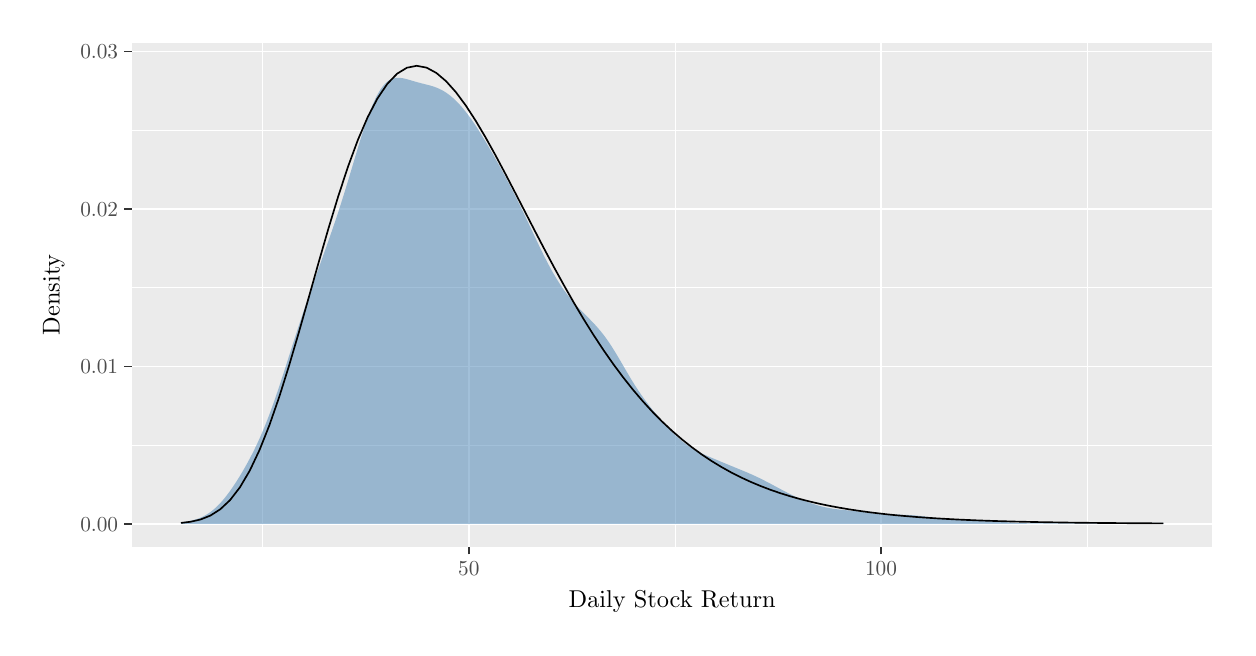
\begin{tikzpicture}[x=1pt,y=1pt]
\definecolor{fillColor}{RGB}{255,255,255}
\path[use as bounding box,fill=fillColor,fill opacity=0.00] (0,0) rectangle (433.62,216.81);
\begin{scope}
\path[clip] (  0.00,  0.00) rectangle (433.62,216.81);
\definecolor{drawColor}{RGB}{255,255,255}
\definecolor{fillColor}{RGB}{255,255,255}

\path[draw=drawColor,line width= 0.6pt,line join=round,line cap=round,fill=fillColor] (  0.00,  0.00) rectangle (433.62,216.81);
\end{scope}
\begin{scope}
\path[clip] ( 37.64, 29.26) rectangle (428.12,211.31);
\definecolor{fillColor}{gray}{0.92}

\path[fill=fillColor] ( 37.64, 29.26) rectangle (428.12,211.31);
\definecolor{drawColor}{RGB}{255,255,255}

\path[draw=drawColor,line width= 0.3pt,line join=round] ( 37.64, 65.97) --
	(428.12, 65.97);

\path[draw=drawColor,line width= 0.3pt,line join=round] ( 37.64,122.84) --
	(428.12,122.84);

\path[draw=drawColor,line width= 0.3pt,line join=round] ( 37.64,179.71) --
	(428.12,179.71);

\path[draw=drawColor,line width= 0.3pt,line join=round] ( 84.90, 29.26) --
	( 84.90,211.31);

\path[draw=drawColor,line width= 0.3pt,line join=round] (233.88, 29.26) --
	(233.88,211.31);

\path[draw=drawColor,line width= 0.3pt,line join=round] (382.87, 29.26) --
	(382.87,211.31);

\path[draw=drawColor,line width= 0.6pt,line join=round] ( 37.64, 37.53) --
	(428.12, 37.53);

\path[draw=drawColor,line width= 0.6pt,line join=round] ( 37.64, 94.40) --
	(428.12, 94.40);

\path[draw=drawColor,line width= 0.6pt,line join=round] ( 37.64,151.28) --
	(428.12,151.28);

\path[draw=drawColor,line width= 0.6pt,line join=round] ( 37.64,208.15) --
	(428.12,208.15);

\path[draw=drawColor,line width= 0.6pt,line join=round] (159.39, 29.26) --
	(159.39,211.31);

\path[draw=drawColor,line width= 0.6pt,line join=round] (308.37, 29.26) --
	(308.37,211.31);
\definecolor{fillColor}{RGB}{70,130,180}

\path[fill=fillColor,fill opacity=0.50] ( 55.39, 38.09) --
	( 56.08, 38.17) --
	( 56.78, 38.26) --
	( 57.47, 38.36) --
	( 58.17, 38.49) --
	( 58.86, 38.63) --
	( 59.56, 38.79) --
	( 60.25, 38.97) --
	( 60.95, 39.18) --
	( 61.64, 39.42) --
	( 62.34, 39.69) --
	( 63.03, 40.00) --
	( 63.73, 40.34) --
	( 64.42, 40.73) --
	( 65.11, 41.16) --
	( 65.81, 41.63) --
	( 66.50, 42.14) --
	( 67.20, 42.70) --
	( 67.89, 43.31) --
	( 68.59, 43.98) --
	( 69.28, 44.68) --
	( 69.98, 45.44) --
	( 70.67, 46.24) --
	( 71.37, 47.08) --
	( 72.06, 47.96) --
	( 72.76, 48.89) --
	( 73.45, 49.86) --
	( 74.15, 50.87) --
	( 74.84, 51.90) --
	( 75.54, 52.98) --
	( 76.23, 54.08) --
	( 76.92, 55.21) --
	( 77.62, 56.38) --
	( 78.31, 57.58) --
	( 79.01, 58.81) --
	( 79.70, 60.08) --
	( 80.40, 61.38) --
	( 81.09, 62.72) --
	( 81.79, 64.11) --
	( 82.48, 65.53) --
	( 83.18, 67.02) --
	( 83.87, 68.55) --
	( 84.57, 70.14) --
	( 85.26, 71.78) --
	( 85.96, 73.48) --
	( 86.65, 75.24) --
	( 87.34, 77.05) --
	( 88.04, 78.93) --
	( 88.73, 80.87) --
	( 89.43, 82.85) --
	( 90.12, 84.88) --
	( 90.82, 86.94) --
	( 91.51, 89.05) --
	( 92.21, 91.18) --
	( 92.90, 93.33) --
	( 93.60, 95.50) --
	( 94.29, 97.68) --
	( 94.99, 99.85) --
	( 95.68,102.03) --
	( 96.38,104.19) --
	( 97.07,106.34) --
	( 97.76,108.47) --
	( 98.46,110.58) --
	( 99.15,112.67) --
	( 99.85,114.73) --
	(100.54,116.78) --
	(101.24,118.80) --
	(101.93,120.81) --
	(102.63,122.80) --
	(103.32,124.77) --
	(104.02,126.72) --
	(104.71,128.67) --
	(105.41,130.62) --
	(106.10,132.55) --
	(106.80,134.49) --
	(107.49,136.44) --
	(108.19,138.39) --
	(108.88,140.36) --
	(109.57,142.35) --
	(110.27,144.36) --
	(110.96,146.40) --
	(111.66,148.47) --
	(112.35,150.57) --
	(113.05,152.72) --
	(113.74,154.91) --
	(114.44,157.13) --
	(115.13,159.39) --
	(115.83,161.68) --
	(116.52,163.99) --
	(117.22,166.32) --
	(117.91,168.65) --
	(118.61,170.98) --
	(119.30,173.29) --
	(119.99,175.57) --
	(120.69,177.81) --
	(121.38,179.98) --
	(122.08,182.08) --
	(122.77,184.09) --
	(123.47,185.98) --
	(124.16,187.77) --
	(124.86,189.42) --
	(125.55,190.95) --
	(126.25,192.35) --
	(126.94,193.60) --
	(127.64,194.70) --
	(128.33,195.64) --
	(129.03,196.45) --
	(129.72,197.11) --
	(130.41,197.65) --
	(131.11,198.07) --
	(131.80,198.38) --
	(132.50,198.59) --
	(133.19,198.69) --
	(133.89,198.71) --
	(134.58,198.67) --
	(135.28,198.58) --
	(135.97,198.45) --
	(136.67,198.28) --
	(137.36,198.09) --
	(138.06,197.89) --
	(138.75,197.69) --
	(139.45,197.48) --
	(140.14,197.28) --
	(140.84,197.09) --
	(141.53,196.90) --
	(142.22,196.72) --
	(142.92,196.55) --
	(143.61,196.37) --
	(144.31,196.20) --
	(145.00,196.02) --
	(145.70,195.82) --
	(146.39,195.61) --
	(147.09,195.38) --
	(147.78,195.12) --
	(148.48,194.83) --
	(149.17,194.50) --
	(149.87,194.14) --
	(150.56,193.73) --
	(151.26,193.29) --
	(151.95,192.81) --
	(152.64,192.28) --
	(153.34,191.70) --
	(154.03,191.08) --
	(154.73,190.42) --
	(155.42,189.72) --
	(156.12,188.98) --
	(156.81,188.20) --
	(157.51,187.38) --
	(158.20,186.51) --
	(158.90,185.61) --
	(159.59,184.68) --
	(160.29,183.71) --
	(160.98,182.71) --
	(161.68,181.68) --
	(162.37,180.63) --
	(163.06,179.55) --
	(163.76,178.44) --
	(164.45,177.31) --
	(165.15,176.16) --
	(165.84,174.99) --
	(166.54,173.81) --
	(167.23,172.61) --
	(167.93,171.40) --
	(168.62,170.18) --
	(169.32,168.94) --
	(170.01,167.69) --
	(170.71,166.43) --
	(171.40,165.16) --
	(172.10,163.87) --
	(172.79,162.57) --
	(173.49,161.26) --
	(174.18,159.93) --
	(174.87,158.59) --
	(175.57,157.23) --
	(176.26,155.86) --
	(176.96,154.47) --
	(177.65,153.06) --
	(178.35,151.64) --
	(179.04,150.20) --
	(179.74,148.75) --
	(180.43,147.28) --
	(181.13,145.81) --
	(181.82,144.33) --
	(182.52,142.85) --
	(183.21,141.37) --
	(183.91,139.89) --
	(184.60,138.43) --
	(185.29,136.99) --
	(185.99,135.56) --
	(186.68,134.16) --
	(187.38,132.79) --
	(188.07,131.45) --
	(188.77,130.15) --
	(189.46,128.89) --
	(190.16,127.68) --
	(190.85,126.50) --
	(191.55,125.36) --
	(192.24,124.27) --
	(192.94,123.22) --
	(193.63,122.21) --
	(194.33,121.25) --
	(195.02,120.32) --
	(195.71,119.43) --
	(196.41,118.57) --
	(197.10,117.74) --
	(197.80,116.95) --
	(198.49,116.18) --
	(199.19,115.43) --
	(199.88,114.71) --
	(200.58,113.99) --
	(201.27,113.29) --
	(201.97,112.59) --
	(202.66,111.90) --
	(203.36,111.19) --
	(204.05,110.48) --
	(204.75,109.74) --
	(205.44,108.99) --
	(206.13,108.20) --
	(206.83,107.38) --
	(207.52,106.53) --
	(208.22,105.64) --
	(208.91,104.70) --
	(209.61,103.72) --
	(210.30,102.70) --
	(211.00,101.64) --
	(211.69,100.54) --
	(212.39, 99.42) --
	(213.08, 98.26) --
	(213.78, 97.09) --
	(214.47, 95.90) --
	(215.17, 94.71) --
	(215.86, 93.51) --
	(216.56, 92.32) --
	(217.25, 91.15) --
	(217.94, 89.99) --
	(218.64, 88.85) --
	(219.33, 87.74) --
	(220.03, 86.66) --
	(220.72, 85.60) --
	(221.42, 84.58) --
	(222.11, 83.58) --
	(222.81, 82.61) --
	(223.50, 81.66) --
	(224.20, 80.75) --
	(224.89, 79.85) --
	(225.59, 78.97) --
	(226.28, 78.11) --
	(226.98, 77.26) --
	(227.67, 76.43) --
	(228.36, 75.61) --
	(229.06, 74.81) --
	(229.75, 74.02) --
	(230.45, 73.25) --
	(231.14, 72.49) --
	(231.84, 71.75) --
	(232.53, 71.03) --
	(233.23, 70.33) --
	(233.92, 69.65) --
	(234.62, 69.00) --
	(235.31, 68.37) --
	(236.01, 67.77) --
	(236.70, 67.20) --
	(237.40, 66.65) --
	(238.09, 66.13) --
	(238.78, 65.65) --
	(239.48, 65.19) --
	(240.17, 64.76) --
	(240.87, 64.35) --
	(241.56, 63.97) --
	(242.26, 63.60) --
	(242.95, 63.25) --
	(243.65, 62.92) --
	(244.34, 62.60) --
	(245.04, 62.29) --
	(245.73, 61.99) --
	(246.43, 61.69) --
	(247.12, 61.40) --
	(247.82, 61.11) --
	(248.51, 60.82) --
	(249.21, 60.53) --
	(249.90, 60.24) --
	(250.59, 59.95) --
	(251.29, 59.66) --
	(251.98, 59.38) --
	(252.68, 59.09) --
	(253.37, 58.80) --
	(254.07, 58.51) --
	(254.76, 58.23) --
	(255.46, 57.94) --
	(256.15, 57.66) --
	(256.85, 57.37) --
	(257.54, 57.09) --
	(258.24, 56.81) --
	(258.93, 56.52) --
	(259.63, 56.23) --
	(260.32, 55.93) --
	(261.01, 55.63) --
	(261.71, 55.32) --
	(262.40, 55.01) --
	(263.10, 54.69) --
	(263.79, 54.36) --
	(264.49, 54.02) --
	(265.18, 53.68) --
	(265.88, 53.33) --
	(266.57, 52.97) --
	(267.27, 52.61) --
	(267.96, 52.25) --
	(268.66, 51.88) --
	(269.35, 51.51) --
	(270.05, 51.13) --
	(270.74, 50.76) --
	(271.43, 50.39) --
	(272.13, 50.02) --
	(272.82, 49.65) --
	(273.52, 49.29) --
	(274.21, 48.93) --
	(274.91, 48.57) --
	(275.60, 48.22) --
	(276.30, 47.88) --
	(276.99, 47.54) --
	(277.69, 47.21) --
	(278.38, 46.89) --
	(279.08, 46.57) --
	(279.77, 46.27) --
	(280.47, 45.98) --
	(281.16, 45.69) --
	(281.86, 45.42) --
	(282.55, 45.16) --
	(283.24, 44.91) --
	(283.94, 44.67) --
	(284.63, 44.45) --
	(285.33, 44.24) --
	(286.02, 44.04) --
	(286.72, 43.86) --
	(287.41, 43.68) --
	(288.11, 43.52) --
	(288.80, 43.38) --
	(289.50, 43.25) --
	(290.19, 43.12) --
	(290.89, 43.01) --
	(291.58, 42.91) --
	(292.28, 42.82) --
	(292.97, 42.73) --
	(293.66, 42.66) --
	(294.36, 42.58) --
	(295.05, 42.51) --
	(295.75, 42.44) --
	(296.44, 42.38) --
	(297.14, 42.31) --
	(297.83, 42.24) --
	(298.53, 42.17) --
	(299.22, 42.09) --
	(299.92, 42.01) --
	(300.61, 41.93) --
	(301.31, 41.85) --
	(302.00, 41.76) --
	(302.70, 41.67) --
	(303.39, 41.58) --
	(304.08, 41.49) --
	(304.78, 41.41) --
	(305.47, 41.32) --
	(306.17, 41.24) --
	(306.86, 41.17) --
	(307.56, 41.10) --
	(308.25, 41.04) --
	(308.95, 40.99) --
	(309.64, 40.95) --
	(310.34, 40.92) --
	(311.03, 40.89) --
	(311.73, 40.87) --
	(312.42, 40.85) --
	(313.12, 40.84) --
	(313.81, 40.83) --
	(314.51, 40.82) --
	(315.20, 40.81) --
	(315.89, 40.80) --
	(316.59, 40.78) --
	(317.28, 40.76) --
	(317.98, 40.73) --
	(318.67, 40.69) --
	(319.37, 40.65) --
	(320.06, 40.60) --
	(320.76, 40.54) --
	(321.45, 40.47) --
	(322.15, 40.40) --
	(322.84, 40.32) --
	(323.54, 40.24) --
	(324.23, 40.15) --
	(324.93, 40.06) --
	(325.62, 39.97) --
	(326.31, 39.88) --
	(327.01, 39.79) --
	(327.70, 39.70) --
	(328.40, 39.61) --
	(329.09, 39.52) --
	(329.79, 39.44) --
	(330.48, 39.37) --
	(331.18, 39.29) --
	(331.87, 39.23) --
	(332.57, 39.16) --
	(333.26, 39.11) --
	(333.96, 39.05) --
	(334.65, 39.01) --
	(335.35, 38.97) --
	(336.04, 38.93) --
	(336.73, 38.90) --
	(337.43, 38.87) --
	(338.12, 38.84) --
	(338.82, 38.82) --
	(339.51, 38.80) --
	(340.21, 38.78) --
	(340.90, 38.76) --
	(341.60, 38.75) --
	(342.29, 38.73) --
	(342.99, 38.71) --
	(343.68, 38.69) --
	(344.38, 38.66) --
	(345.07, 38.64) --
	(345.77, 38.61) --
	(346.46, 38.58) --
	(347.16, 38.54) --
	(347.85, 38.51) --
	(348.54, 38.47) --
	(349.24, 38.42) --
	(349.93, 38.38) --
	(350.63, 38.33) --
	(351.32, 38.28) --
	(352.02, 38.23) --
	(352.71, 38.18) --
	(353.41, 38.13) --
	(354.10, 38.09) --
	(354.80, 38.04) --
	(355.49, 37.99) --
	(356.19, 37.95) --
	(356.88, 37.91) --
	(357.58, 37.87) --
	(358.27, 37.84) --
	(358.96, 37.80) --
	(359.66, 37.78) --
	(360.35, 37.75) --
	(361.05, 37.73) --
	(361.74, 37.72) --
	(362.44, 37.70) --
	(363.13, 37.69) --
	(363.83, 37.69) --
	(364.52, 37.68) --
	(365.22, 37.68) --
	(365.91, 37.68) --
	(366.61, 37.68) --
	(367.30, 37.69) --
	(368.00, 37.69) --
	(368.69, 37.70) --
	(369.38, 37.70) --
	(370.08, 37.71) --
	(370.77, 37.72) --
	(371.47, 37.72) --
	(372.16, 37.73) --
	(372.86, 37.73) --
	(373.55, 37.73) --
	(374.25, 37.73) --
	(374.94, 37.73) --
	(375.64, 37.73) --
	(376.33, 37.73) --
	(377.03, 37.73) --
	(377.72, 37.72) --
	(378.42, 37.72) --
	(379.11, 37.71) --
	(379.81, 37.71) --
	(380.50, 37.71) --
	(381.19, 37.70) --
	(381.89, 37.70) --
	(382.58, 37.70) --
	(383.28, 37.70) --
	(383.97, 37.71) --
	(384.67, 37.71) --
	(385.36, 37.72) --
	(386.06, 37.72) --
	(386.75, 37.73) --
	(387.45, 37.74) --
	(388.14, 37.75) --
	(388.84, 37.76) --
	(389.53, 37.77) --
	(390.23, 37.78) --
	(390.92, 37.79) --
	(391.61, 37.79) --
	(392.31, 37.80) --
	(393.00, 37.81) --
	(393.70, 37.82) --
	(394.39, 37.83) --
	(395.09, 37.84) --
	(395.78, 37.85) --
	(396.48, 37.85) --
	(397.17, 37.86) --
	(397.87, 37.87) --
	(398.56, 37.87) --
	(399.26, 37.88) --
	(399.95, 37.88) --
	(400.65, 37.89) --
	(401.34, 37.89) --
	(402.03, 37.89) --
	(402.73, 37.89) --
	(403.42, 37.89) --
	(404.12, 37.89) --
	(404.81, 37.89) --
	(405.51, 37.89) --
	(406.20, 37.89) --
	(406.90, 37.88) --
	(407.59, 37.88) --
	(408.29, 37.87) --
	(408.98, 37.86) --
	(409.68, 37.85) --
	(410.37, 37.83) --
	(410.37, 37.53) --
	(409.68, 37.53) --
	(408.98, 37.53) --
	(408.29, 37.53) --
	(407.59, 37.53) --
	(406.90, 37.53) --
	(406.20, 37.53) --
	(405.51, 37.53) --
	(404.81, 37.53) --
	(404.12, 37.53) --
	(403.42, 37.53) --
	(402.73, 37.53) --
	(402.03, 37.53) --
	(401.34, 37.53) --
	(400.65, 37.53) --
	(399.95, 37.53) --
	(399.26, 37.53) --
	(398.56, 37.53) --
	(397.87, 37.53) --
	(397.17, 37.53) --
	(396.48, 37.53) --
	(395.78, 37.53) --
	(395.09, 37.53) --
	(394.39, 37.53) --
	(393.70, 37.53) --
	(393.00, 37.53) --
	(392.31, 37.53) --
	(391.61, 37.53) --
	(390.92, 37.53) --
	(390.23, 37.53) --
	(389.53, 37.53) --
	(388.84, 37.53) --
	(388.14, 37.53) --
	(387.45, 37.53) --
	(386.75, 37.53) --
	(386.06, 37.53) --
	(385.36, 37.53) --
	(384.67, 37.53) --
	(383.97, 37.53) --
	(383.28, 37.53) --
	(382.58, 37.53) --
	(381.89, 37.53) --
	(381.19, 37.53) --
	(380.50, 37.53) --
	(379.81, 37.53) --
	(379.11, 37.53) --
	(378.42, 37.53) --
	(377.72, 37.53) --
	(377.03, 37.53) --
	(376.33, 37.53) --
	(375.64, 37.53) --
	(374.94, 37.53) --
	(374.25, 37.53) --
	(373.55, 37.53) --
	(372.86, 37.53) --
	(372.16, 37.53) --
	(371.47, 37.53) --
	(370.77, 37.53) --
	(370.08, 37.53) --
	(369.38, 37.53) --
	(368.69, 37.53) --
	(368.00, 37.53) --
	(367.30, 37.53) --
	(366.61, 37.53) --
	(365.91, 37.53) --
	(365.22, 37.53) --
	(364.52, 37.53) --
	(363.83, 37.53) --
	(363.13, 37.53) --
	(362.44, 37.53) --
	(361.74, 37.53) --
	(361.05, 37.53) --
	(360.35, 37.53) --
	(359.66, 37.53) --
	(358.96, 37.53) --
	(358.27, 37.53) --
	(357.58, 37.53) --
	(356.88, 37.53) --
	(356.19, 37.53) --
	(355.49, 37.53) --
	(354.80, 37.53) --
	(354.10, 37.53) --
	(353.41, 37.53) --
	(352.71, 37.53) --
	(352.02, 37.53) --
	(351.32, 37.53) --
	(350.63, 37.53) --
	(349.93, 37.53) --
	(349.24, 37.53) --
	(348.54, 37.53) --
	(347.85, 37.53) --
	(347.16, 37.53) --
	(346.46, 37.53) --
	(345.77, 37.53) --
	(345.07, 37.53) --
	(344.38, 37.53) --
	(343.68, 37.53) --
	(342.99, 37.53) --
	(342.29, 37.53) --
	(341.60, 37.53) --
	(340.90, 37.53) --
	(340.21, 37.53) --
	(339.51, 37.53) --
	(338.82, 37.53) --
	(338.12, 37.53) --
	(337.43, 37.53) --
	(336.73, 37.53) --
	(336.04, 37.53) --
	(335.35, 37.53) --
	(334.65, 37.53) --
	(333.96, 37.53) --
	(333.26, 37.53) --
	(332.57, 37.53) --
	(331.87, 37.53) --
	(331.18, 37.53) --
	(330.48, 37.53) --
	(329.79, 37.53) --
	(329.09, 37.53) --
	(328.40, 37.53) --
	(327.70, 37.53) --
	(327.01, 37.53) --
	(326.31, 37.53) --
	(325.62, 37.53) --
	(324.93, 37.53) --
	(324.23, 37.53) --
	(323.54, 37.53) --
	(322.84, 37.53) --
	(322.15, 37.53) --
	(321.45, 37.53) --
	(320.76, 37.53) --
	(320.06, 37.53) --
	(319.37, 37.53) --
	(318.67, 37.53) --
	(317.98, 37.53) --
	(317.28, 37.53) --
	(316.59, 37.53) --
	(315.89, 37.53) --
	(315.20, 37.53) --
	(314.51, 37.53) --
	(313.81, 37.53) --
	(313.12, 37.53) --
	(312.42, 37.53) --
	(311.73, 37.53) --
	(311.03, 37.53) --
	(310.34, 37.53) --
	(309.64, 37.53) --
	(308.95, 37.53) --
	(308.25, 37.53) --
	(307.56, 37.53) --
	(306.86, 37.53) --
	(306.17, 37.53) --
	(305.47, 37.53) --
	(304.78, 37.53) --
	(304.08, 37.53) --
	(303.39, 37.53) --
	(302.70, 37.53) --
	(302.00, 37.53) --
	(301.31, 37.53) --
	(300.61, 37.53) --
	(299.92, 37.53) --
	(299.22, 37.53) --
	(298.53, 37.53) --
	(297.83, 37.53) --
	(297.14, 37.53) --
	(296.44, 37.53) --
	(295.75, 37.53) --
	(295.05, 37.53) --
	(294.36, 37.53) --
	(293.66, 37.53) --
	(292.97, 37.53) --
	(292.28, 37.53) --
	(291.58, 37.53) --
	(290.89, 37.53) --
	(290.19, 37.53) --
	(289.50, 37.53) --
	(288.80, 37.53) --
	(288.11, 37.53) --
	(287.41, 37.53) --
	(286.72, 37.53) --
	(286.02, 37.53) --
	(285.33, 37.53) --
	(284.63, 37.53) --
	(283.94, 37.53) --
	(283.24, 37.53) --
	(282.55, 37.53) --
	(281.86, 37.53) --
	(281.16, 37.53) --
	(280.47, 37.53) --
	(279.77, 37.53) --
	(279.08, 37.53) --
	(278.38, 37.53) --
	(277.69, 37.53) --
	(276.99, 37.53) --
	(276.30, 37.53) --
	(275.60, 37.53) --
	(274.91, 37.53) --
	(274.21, 37.53) --
	(273.52, 37.53) --
	(272.82, 37.53) --
	(272.13, 37.53) --
	(271.43, 37.53) --
	(270.74, 37.53) --
	(270.05, 37.53) --
	(269.35, 37.53) --
	(268.66, 37.53) --
	(267.96, 37.53) --
	(267.27, 37.53) --
	(266.57, 37.53) --
	(265.88, 37.53) --
	(265.18, 37.53) --
	(264.49, 37.53) --
	(263.79, 37.53) --
	(263.10, 37.53) --
	(262.40, 37.53) --
	(261.71, 37.53) --
	(261.01, 37.53) --
	(260.32, 37.53) --
	(259.63, 37.53) --
	(258.93, 37.53) --
	(258.24, 37.53) --
	(257.54, 37.53) --
	(256.85, 37.53) --
	(256.15, 37.53) --
	(255.46, 37.53) --
	(254.76, 37.53) --
	(254.07, 37.53) --
	(253.37, 37.53) --
	(252.68, 37.53) --
	(251.98, 37.53) --
	(251.29, 37.53) --
	(250.59, 37.53) --
	(249.90, 37.53) --
	(249.21, 37.53) --
	(248.51, 37.53) --
	(247.82, 37.53) --
	(247.12, 37.53) --
	(246.43, 37.53) --
	(245.73, 37.53) --
	(245.04, 37.53) --
	(244.34, 37.53) --
	(243.65, 37.53) --
	(242.95, 37.53) --
	(242.26, 37.53) --
	(241.56, 37.53) --
	(240.87, 37.53) --
	(240.17, 37.53) --
	(239.48, 37.53) --
	(238.78, 37.53) --
	(238.09, 37.53) --
	(237.40, 37.53) --
	(236.70, 37.53) --
	(236.01, 37.53) --
	(235.31, 37.53) --
	(234.62, 37.53) --
	(233.92, 37.53) --
	(233.23, 37.53) --
	(232.53, 37.53) --
	(231.84, 37.53) --
	(231.14, 37.53) --
	(230.45, 37.53) --
	(229.75, 37.53) --
	(229.06, 37.53) --
	(228.36, 37.53) --
	(227.67, 37.53) --
	(226.98, 37.53) --
	(226.28, 37.53) --
	(225.59, 37.53) --
	(224.89, 37.53) --
	(224.20, 37.53) --
	(223.50, 37.53) --
	(222.81, 37.53) --
	(222.11, 37.53) --
	(221.42, 37.53) --
	(220.72, 37.53) --
	(220.03, 37.53) --
	(219.33, 37.53) --
	(218.64, 37.53) --
	(217.94, 37.53) --
	(217.25, 37.53) --
	(216.56, 37.53) --
	(215.86, 37.53) --
	(215.17, 37.53) --
	(214.47, 37.53) --
	(213.78, 37.53) --
	(213.08, 37.53) --
	(212.39, 37.53) --
	(211.69, 37.53) --
	(211.00, 37.53) --
	(210.30, 37.53) --
	(209.61, 37.53) --
	(208.91, 37.53) --
	(208.22, 37.53) --
	(207.52, 37.53) --
	(206.83, 37.53) --
	(206.13, 37.53) --
	(205.44, 37.53) --
	(204.75, 37.53) --
	(204.05, 37.53) --
	(203.36, 37.53) --
	(202.66, 37.53) --
	(201.97, 37.53) --
	(201.27, 37.53) --
	(200.58, 37.53) --
	(199.88, 37.53) --
	(199.19, 37.53) --
	(198.49, 37.53) --
	(197.80, 37.53) --
	(197.10, 37.53) --
	(196.41, 37.53) --
	(195.71, 37.53) --
	(195.02, 37.53) --
	(194.33, 37.53) --
	(193.63, 37.53) --
	(192.94, 37.53) --
	(192.24, 37.53) --
	(191.55, 37.53) --
	(190.85, 37.53) --
	(190.16, 37.53) --
	(189.46, 37.53) --
	(188.77, 37.53) --
	(188.07, 37.53) --
	(187.38, 37.53) --
	(186.68, 37.53) --
	(185.99, 37.53) --
	(185.29, 37.53) --
	(184.60, 37.53) --
	(183.91, 37.53) --
	(183.21, 37.53) --
	(182.52, 37.53) --
	(181.82, 37.53) --
	(181.13, 37.53) --
	(180.43, 37.53) --
	(179.74, 37.53) --
	(179.04, 37.53) --
	(178.35, 37.53) --
	(177.65, 37.53) --
	(176.96, 37.53) --
	(176.26, 37.53) --
	(175.57, 37.53) --
	(174.87, 37.53) --
	(174.18, 37.53) --
	(173.49, 37.53) --
	(172.79, 37.53) --
	(172.10, 37.53) --
	(171.40, 37.53) --
	(170.71, 37.53) --
	(170.01, 37.53) --
	(169.32, 37.53) --
	(168.62, 37.53) --
	(167.93, 37.53) --
	(167.23, 37.53) --
	(166.54, 37.53) --
	(165.84, 37.53) --
	(165.15, 37.53) --
	(164.45, 37.53) --
	(163.76, 37.53) --
	(163.06, 37.53) --
	(162.37, 37.53) --
	(161.68, 37.53) --
	(160.98, 37.53) --
	(160.29, 37.53) --
	(159.59, 37.53) --
	(158.90, 37.53) --
	(158.20, 37.53) --
	(157.51, 37.53) --
	(156.81, 37.53) --
	(156.12, 37.53) --
	(155.42, 37.53) --
	(154.73, 37.53) --
	(154.03, 37.53) --
	(153.34, 37.53) --
	(152.64, 37.53) --
	(151.95, 37.53) --
	(151.26, 37.53) --
	(150.56, 37.53) --
	(149.87, 37.53) --
	(149.17, 37.53) --
	(148.48, 37.53) --
	(147.78, 37.53) --
	(147.09, 37.53) --
	(146.39, 37.53) --
	(145.70, 37.53) --
	(145.00, 37.53) --
	(144.31, 37.53) --
	(143.61, 37.53) --
	(142.92, 37.53) --
	(142.22, 37.53) --
	(141.53, 37.53) --
	(140.84, 37.53) --
	(140.14, 37.53) --
	(139.45, 37.53) --
	(138.75, 37.53) --
	(138.06, 37.53) --
	(137.36, 37.53) --
	(136.67, 37.53) --
	(135.97, 37.53) --
	(135.28, 37.53) --
	(134.58, 37.53) --
	(133.89, 37.53) --
	(133.19, 37.53) --
	(132.50, 37.53) --
	(131.80, 37.53) --
	(131.11, 37.53) --
	(130.41, 37.53) --
	(129.72, 37.53) --
	(129.03, 37.53) --
	(128.33, 37.53) --
	(127.64, 37.53) --
	(126.94, 37.53) --
	(126.25, 37.53) --
	(125.55, 37.53) --
	(124.86, 37.53) --
	(124.16, 37.53) --
	(123.47, 37.53) --
	(122.77, 37.53) --
	(122.08, 37.53) --
	(121.38, 37.53) --
	(120.69, 37.53) --
	(119.99, 37.53) --
	(119.30, 37.53) --
	(118.61, 37.53) --
	(117.91, 37.53) --
	(117.22, 37.53) --
	(116.52, 37.53) --
	(115.83, 37.53) --
	(115.13, 37.53) --
	(114.44, 37.53) --
	(113.74, 37.53) --
	(113.05, 37.53) --
	(112.35, 37.53) --
	(111.66, 37.53) --
	(110.96, 37.53) --
	(110.27, 37.53) --
	(109.57, 37.53) --
	(108.88, 37.53) --
	(108.19, 37.53) --
	(107.49, 37.53) --
	(106.80, 37.53) --
	(106.10, 37.53) --
	(105.41, 37.53) --
	(104.71, 37.53) --
	(104.02, 37.53) --
	(103.32, 37.53) --
	(102.63, 37.53) --
	(101.93, 37.53) --
	(101.24, 37.53) --
	(100.54, 37.53) --
	( 99.85, 37.53) --
	( 99.15, 37.53) --
	( 98.46, 37.53) --
	( 97.76, 37.53) --
	( 97.07, 37.53) --
	( 96.38, 37.53) --
	( 95.68, 37.53) --
	( 94.99, 37.53) --
	( 94.29, 37.53) --
	( 93.60, 37.53) --
	( 92.90, 37.53) --
	( 92.21, 37.53) --
	( 91.51, 37.53) --
	( 90.82, 37.53) --
	( 90.12, 37.53) --
	( 89.43, 37.53) --
	( 88.73, 37.53) --
	( 88.04, 37.53) --
	( 87.34, 37.53) --
	( 86.65, 37.53) --
	( 85.96, 37.53) --
	( 85.26, 37.53) --
	( 84.57, 37.53) --
	( 83.87, 37.53) --
	( 83.18, 37.53) --
	( 82.48, 37.53) --
	( 81.79, 37.53) --
	( 81.09, 37.53) --
	( 80.40, 37.53) --
	( 79.70, 37.53) --
	( 79.01, 37.53) --
	( 78.31, 37.53) --
	( 77.62, 37.53) --
	( 76.92, 37.53) --
	( 76.23, 37.53) --
	( 75.54, 37.53) --
	( 74.84, 37.53) --
	( 74.15, 37.53) --
	( 73.45, 37.53) --
	( 72.76, 37.53) --
	( 72.06, 37.53) --
	( 71.37, 37.53) --
	( 70.67, 37.53) --
	( 69.98, 37.53) --
	( 69.28, 37.53) --
	( 68.59, 37.53) --
	( 67.89, 37.53) --
	( 67.20, 37.53) --
	( 66.50, 37.53) --
	( 65.81, 37.53) --
	( 65.11, 37.53) --
	( 64.42, 37.53) --
	( 63.73, 37.53) --
	( 63.03, 37.53) --
	( 62.34, 37.53) --
	( 61.64, 37.53) --
	( 60.95, 37.53) --
	( 60.25, 37.53) --
	( 59.56, 37.53) --
	( 58.86, 37.53) --
	( 58.17, 37.53) --
	( 57.47, 37.53) --
	( 56.78, 37.53) --
	( 56.08, 37.53) --
	( 55.39, 37.53) --
	cycle;
\definecolor{drawColor}{RGB}{0,0,0}

\path[draw=drawColor,line width= 0.6pt,line join=round] ( 55.39, 37.85) --
	( 58.94, 38.28) --
	( 62.49, 39.10) --
	( 66.04, 40.52) --
	( 69.59, 42.78) --
	( 73.14, 46.11) --
	( 76.69, 50.71) --
	( 80.24, 56.73) --
	( 83.79, 64.22) --
	( 87.34, 73.14) --
	( 90.89, 83.36) --
	( 94.44, 94.65) --
	( 97.99,106.71) --
	(101.54,119.22) --
	(105.09,131.80) --
	(108.64,144.10) --
	(112.19,155.78) --
	(115.74,166.55) --
	(119.29,176.17) --
	(122.84,184.43) --
	(126.39,191.23) --
	(129.94,196.48) --
	(133.49,200.18) --
	(137.04,202.34) --
	(140.58,203.03) --
	(144.13,202.37) --
	(147.68,200.45) --
	(151.23,197.43) --
	(154.78,193.45) --
	(158.33,188.66) --
	(161.88,183.19) --
	(165.43,177.20) --
	(168.98,170.82) --
	(172.53,164.15) --
	(176.08,157.32) --
	(179.63,150.43) --
	(183.18,143.54) --
	(186.73,136.74) --
	(190.28,130.09) --
	(193.83,123.63) --
	(197.38,117.40) --
	(200.93,111.43) --
	(204.48,105.75) --
	(208.03,100.36) --
	(211.58, 95.28) --
	(215.13, 90.51) --
	(218.68, 86.04) --
	(222.23, 81.87) --
	(225.78, 77.99) --
	(229.33, 74.40) --
	(232.88, 71.08) --
	(236.43, 68.02) --
	(239.98, 65.21) --
	(243.53, 62.62) --
	(247.08, 60.25) --
	(250.63, 58.09) --
	(254.18, 56.11) --
	(257.73, 54.31) --
	(261.28, 52.67) --
	(264.83, 51.19) --
	(268.38, 49.83) --
	(271.93, 48.61) --
	(275.48, 47.50) --
	(279.03, 46.50) --
	(282.58, 45.59) --
	(286.13, 44.77) --
	(289.68, 44.03) --
	(293.23, 43.37) --
	(296.78, 42.77) --
	(300.33, 42.23) --
	(303.88, 41.74) --
	(307.43, 41.31) --
	(310.98, 40.91) --
	(314.53, 40.56) --
	(318.08, 40.25) --
	(321.63, 39.96) --
	(325.18, 39.71) --
	(328.73, 39.48) --
	(332.27, 39.28) --
	(335.82, 39.09) --
	(339.37, 38.93) --
	(342.92, 38.78) --
	(346.47, 38.65) --
	(350.02, 38.53) --
	(353.57, 38.43) --
	(357.12, 38.33) --
	(360.67, 38.25) --
	(364.22, 38.17) --
	(367.77, 38.11) --
	(371.32, 38.05) --
	(374.87, 37.99) --
	(378.42, 37.94) --
	(381.97, 37.90) --
	(385.52, 37.86) --
	(389.07, 37.83) --
	(392.62, 37.80) --
	(396.17, 37.77) --
	(399.72, 37.74) --
	(403.27, 37.72) --
	(406.82, 37.70) --
	(410.37, 37.68);
\end{scope}
\begin{scope}
\path[clip] (  0.00,  0.00) rectangle (433.62,216.81);
\definecolor{drawColor}{gray}{0.30}

\node[text=drawColor,anchor=base east,inner sep=0pt, outer sep=0pt, scale=  0.77] at ( 32.69, 34.88) {0.00};

\node[text=drawColor,anchor=base east,inner sep=0pt, outer sep=0pt, scale=  0.77] at ( 32.69, 91.75) {0.01};

\node[text=drawColor,anchor=base east,inner sep=0pt, outer sep=0pt, scale=  0.77] at ( 32.69,148.63) {0.02};

\node[text=drawColor,anchor=base east,inner sep=0pt, outer sep=0pt, scale=  0.77] at ( 32.69,205.50) {0.03};
\end{scope}
\begin{scope}
\path[clip] (  0.00,  0.00) rectangle (433.62,216.81);
\definecolor{drawColor}{gray}{0.20}

\path[draw=drawColor,line width= 0.6pt,line join=round] ( 34.89, 37.53) --
	( 37.64, 37.53);

\path[draw=drawColor,line width= 0.6pt,line join=round] ( 34.89, 94.40) --
	( 37.64, 94.40);

\path[draw=drawColor,line width= 0.6pt,line join=round] ( 34.89,151.28) --
	( 37.64,151.28);

\path[draw=drawColor,line width= 0.6pt,line join=round] ( 34.89,208.15) --
	( 37.64,208.15);
\end{scope}
\begin{scope}
\path[clip] (  0.00,  0.00) rectangle (433.62,216.81);
\definecolor{drawColor}{gray}{0.20}

\path[draw=drawColor,line width= 0.6pt,line join=round] (159.39, 26.51) --
	(159.39, 29.26);

\path[draw=drawColor,line width= 0.6pt,line join=round] (308.37, 26.51) --
	(308.37, 29.26);
\end{scope}
\begin{scope}
\path[clip] (  0.00,  0.00) rectangle (433.62,216.81);
\definecolor{drawColor}{gray}{0.30}

\node[text=drawColor,anchor=base,inner sep=0pt, outer sep=0pt, scale=  0.77] at (159.39, 19.00) {50};

\node[text=drawColor,anchor=base,inner sep=0pt, outer sep=0pt, scale=  0.77] at (308.37, 19.00) {100};
\end{scope}
\begin{scope}
\path[clip] (  0.00,  0.00) rectangle (433.62,216.81);
\definecolor{drawColor}{RGB}{0,0,0}

\node[text=drawColor,anchor=base,inner sep=0pt, outer sep=0pt, scale=  0.88] at (232.88,  7.44) {Daily Stock Return};
\end{scope}
\begin{scope}
\path[clip] (  0.00,  0.00) rectangle (433.62,216.81);
\definecolor{drawColor}{RGB}{0,0,0}

\node[text=drawColor,rotate= 90.00,anchor=base,inner sep=0pt, outer sep=0pt, scale=  0.88] at ( 11.56,120.28) {Density};
\end{scope}
\end{tikzpicture}

\caption{Daily Basis Stock Return Density}
\label{p:logdensity}
\floatfoot{
The above density function has been constructed over three distinctive groups of 10000 samples eachs. All samples have been constructed following \cref{eq:Scontinuous}. The arguments are set with the following value, $\alpha = 0$, $\sigma = 30\%$. The black density belongs to the log--normal curve with mean and standard deviation such as described in [REF]. The time frame is one year ($t = 1$) and period between each measure, namely $dt$ has been set to $500^{-1}$. 
}
\end{figure}

%%%%%%%%%%%%%%%%%%%%%%%%%%%%%%%%%%%%%%%%%%%%%%%%
% SUBSECTION: Flaws
%%%%%%%%%%%%%%%%%%%%%%%%%%%%%%%%%%%%%%%%%%%%%%%%
\section{Flaws}
\label{sec:Flaws}

Even if the \cref{eq:Scontinuous} is used to model the stock price process, it exists some lacks with the observed real processes. The analysis ([CHA REF]) mainly covers the following discrepancy of the model against empirical results.
  
The volatility appearing in the aformentioned underlying model (\ref{eq:Scontinuous}) is constant as time passes.
Even if this consideration can be considered as true for short period of time, it is not the case over the long--run \citet{teneng2011limitations}.
Other model substitutes the process defined throughout this chapter with other ones including stochastic volatility processes, making it changing over time.
For this purpose, the Heston's model is developed in this current master thesis, which encompasses two stochastic processes, a geometric Brownian motion [???? + REF] for the stock price diffusion model [DIFUSION??] and a mean-reverting CIR model to compute the volatility as a stochastic process.
This model is exposed in \cref{sec:Heston}.

Following [REF and REF], the uderlying log--returns distribution is characterized by the normal law. Consequently, the random variable $\St$, at the fixed time $t$, is normal. 
However, according to empirical results, the random variable $d\St$ do not fit with the normal bell curve (\citet{clark1973}).
Therefore if the price changes are not normally distribution neither is the log--return and thus $\St$, at a fixed time $t$, is not log--normally distributed.
Along with the Heston model, another one is considerd; the Merton's jump--diffusion model. Both are able to modify the skewness and kurtosis of the log--return distibution curve. The Merton framework is developed in \cref{sec:MixedJump}. 
%%%%%%%%%%%%%%%%%%%%%%%%%%%%%%%%%%%%%%%%%%%%%%%%%%%%%%%%%%%%%%%%%%%%%%%%%%%%%%%%
%
%  CHAPTER:The \BSM model
%
%%%%%%%%%%%%%%%%%%%%%%%%%%%%%%%%%%%%%%%%%%%%%%%%%%%%%%%%%%%%%%%%%%%%%%%%%%%%%%%%
\chapter{The \BSM model}
\label{cha:bsm}


%%%%%%%%%%%%%%%%%%%%%%%%%%%%%%%%%%%%%%%%%%%%%%%%
% SECTION: OverView
%%%%%%%%%%%%%%%%%%%%%%%%%%%%%%%%%%%%%%%%%%%%%%%%
\section{Overview}
\label{sec:bsm:overview}

In this present section the Black--Scholes--Merton model is explained and developed. Stricly speaking, it would be talked about the BSM (Black--Scholes--Merton) model but not BSM equation. In turn the equation would be refered to as the BS (Black and Scholes) equation. This distinction is made because the model encompasses the derivation of the BS equation, either using the CAPM (Capital Asset Pricing Model) for \citet{bs} or  by setting up a riskless portfolio providing an expected return identiacal to risk-free rate for \citet{merton73}.

The BSM model is meant to provide the non arbitrage price of derivative assets such as european stock option (\citet{hull}). In the present master thesis the model derived from the BS formula is focused on the pricing of one of a kind trivial derivative, the vanilla call option.

In order to price call option throughout the model highlighted in this present chapter, some contraints have been set by \citet{bs}. 
The section \ref{sec:Assumptions} quotes the assumptions made to keep the model usage between boundaries. In latter chapter however it will be shown how the model is relevant by going on the edge and even beyond these constraints.


%%%%%%%%%%%%%%%%%%%%%%%%%%%%%%%%%%%%%%%%%%%%%%%%
% SECTION: Assumptions
%%%%%%%%%%%%%%%%%%%%%%%%%%%%%%%%%%%%%%%%%%%%%%%%
\section{Assumptions}
\label{sec:bsm:assumptions}

\citet{bs} have provided a framework defining a bunch of constraints qualified as "ideal conditions" under which the market would behave in order to make the BS equation works with accuracy. All of these conditions are below--mentioned.

\begin{enumerate}
  \item The short-term risk free rate $r$ is known and constant
  \item The stock return involving in the computation of BS equation is lognormally distributed with constant mean and variance rate
  \item No dividend are provided with the considered share of stock
  \item The option considered within the computation is european
  \item The price for bid and ask quote are identical. It means that there is no bid--ask spread to be considerered
  \item Share of stock can be divided into any portions such as needed for the computation
  \item Short selling is allowed with no penalties
\end{enumerate}


%%%%%%%%%%%%%%%%%%%%%%%%%%%%%%%%%%%%%%%%%%%%%%%%
% SECTION: The partial differential BSM equation
%%%%%%%%%%%%%%%%%%%%%%%%%%%%%%%%%%%%%%%%%%%%%%%%
\section{The \BSM equation}
\label{sec:bsm:equation}

The pricing method of an option underpinned by the BSM model is closely related to an underlying for which its price $\St$ is random and log--normally distributed, such the one developed in chapter \ref{cha:underlying} throughout equation \ref{eq:Scontinuous} (\citet{bs}).

In order to provide a unique fair price to a stock option (e.g. a vanilla european call option) which depends on an underlying such as described above, all the uncertainty associated to the stock price motion has to disappear. To do so, one have to first construct such a portofolio $X(t)$ which encompasses the same source on uncertainty as the option itself, i.e., the geometric brownian motion $\St$ and then choosing the adequate position $\Delta(t)$ to take  so that all randomness cancels out (\citet{shreve}).
 
\begin{align}
  \dportfolio \label{eq:dportfolio} \\ 
  \intertext{The goal is to hedge dynamically the position taken in the option. It means that the position has to be frequently rebalanced. Consequently, at any times, the present value of the changes occuring in the portfolio, due to stock price evolution should be equal to the one occuring in the derivative. The only way to achieve this equality is to adapt the delta (\citet{shreve}).}
   d\left(e^{-rt} X\left(t\right)\right) &= d\left(e^{-rt} \ct \right)
\intertext{In that way, one can take a position in the derivatives (short / long) and hedge them by taking $\pm \Delta(t)$ shares of stock. $X(0)$ being the price of the call at time zero}
 X\left(0\right) &= c\left(0, S\left(0\right)\right)
\end{align}




Following the method forementioned, the BSM differential equation is given by equation (\ref{eq:bsm:bsm:eq}),  with terminal condition (\ref{eq:BSMterminal}) and boundary condition (\ref{eq:BSMboundary0}) -- (\ref{eq:BSMboundaryinf}), (\citet{shreve}).

\begin{center}
  \begin{equation}
     \BSMeq{x}
    \label{eq:bsm:bsm:eq}
  \end{equation}
\end{center}
 
\begin{center}
  \begin{equation}
    \call{T}{x} = \left(x - K\right) ^+
    \label{eq:BSMterminal}
  \end{equation}
\end{center}

Whilst the terminal condition focuses on the value taken at maturity, the boundary conditions fix some constraints on the extreme values likely to be taken by the shares of stock at any times during the option life. 
In that regard, the boundary condition (\ref{eq:BSMboundary0}) shows that an option with an worthless underlying is itself valueless, while whenever the option is deep in the money, simulated with $x = \infty$ (\ref{eq:BSMboundaryinf}), the value of the derivative is equal to the value of a forward contract involving the same underlying and with the same maturity date.

\begin{center}
  \begin{equation}
    \call{t}{0} = 0
    \label{eq:BSMboundary0}
  \end{equation}
\end{center}

\begin{center}
  \begin{equation}
    \lim_{x\to\infty} \left[ \call{t}{x} - \left(x - e^{-r \left(T - t \right)} \right) \right] = 0
    \label{eq:BSMboundaryinf}
  \end{equation}
\end{center}
 
%%%%%%%%%%%%%%%%%%%%%%%%%%%%%%%%%%%%%%%%%%%%%%%%
% SECTION: Solution for vanilla option pricing method
%%%%%%%%%%%%%%%%%%%%%%%%%%%%%%%%%%%%%%%%%%%%%%%%
\section{Solution for vanilla option pricing method}
\label{sec:Solution for vanilla option pricing method}


According to the terminal (\ref{eq:BSMterminal}) and boundaries conditions (\ref{eq:BSMboundary0}, \ref{eq:BSMboundaryinf}), the Black--Scholes--Merton solution for call option happens to be given by equation (\ref{eq:bsm:bsm:sol}), (\citet{shreve}). 
The right hand side of the equation, $\ct$, denotes the price of a call option depending on the time to maturity and the stock price at that time.
In addition to these arguments, two other parameters are required, the strike ($k$) and the riskless interest rate ($r$).

\begin{align}
    \BSMsol
    \label{eq:bsm:bsm:sol}
\intertext{with}
    \dpm
    \label{eq:dpm}
\end{align}








% \begin{figure}[!h]
% \centering
% % Created by tikzDevice version 0.11 on 2018-04-08 08:39:42
% !TEX encoding = UTF-8 Unicode
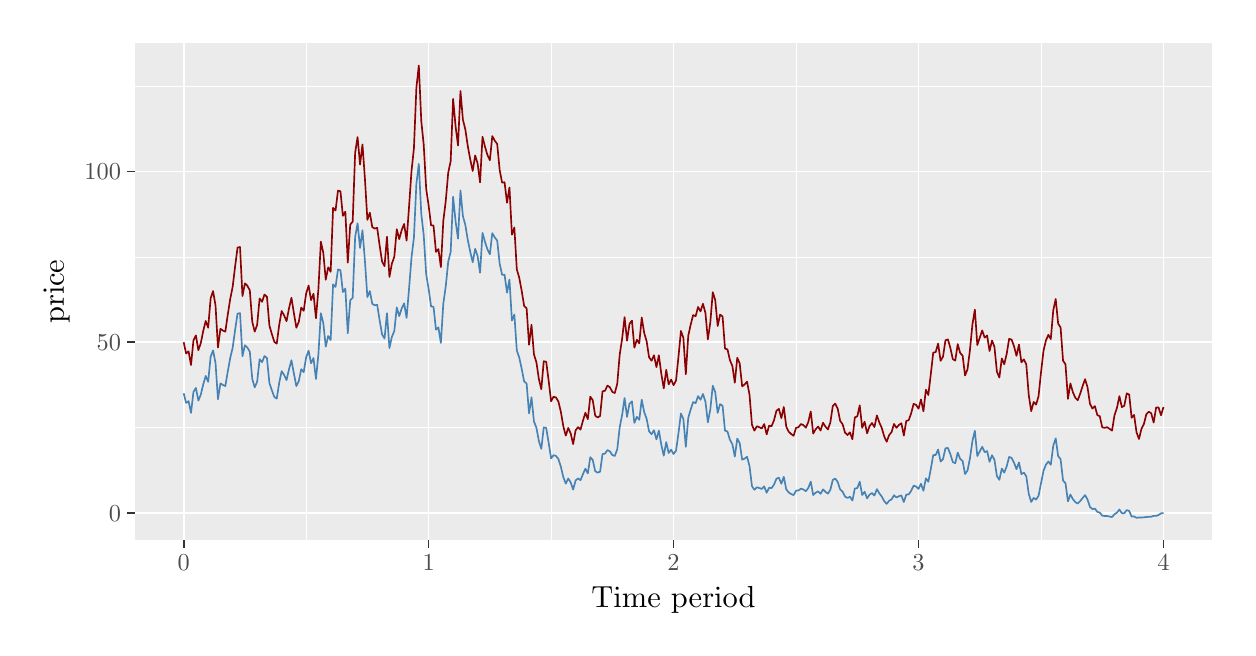
\begin{tikzpicture}[x=1pt,y=1pt]
\definecolor{fillColor}{RGB}{255,255,255}
\path[use as bounding box,fill=fillColor,fill opacity=0.00] (0,0) rectangle (433.62,216.81);
\begin{scope}
\path[clip] (  0.00,  0.00) rectangle (433.62,216.81);
\definecolor{drawColor}{RGB}{255,255,255}
\definecolor{fillColor}{RGB}{255,255,255}

\path[draw=drawColor,line width= 0.6pt,line join=round,line cap=round,fill=fillColor] (  0.00,  0.00) rectangle (433.62,216.81);
\end{scope}
\begin{scope}
\path[clip] ( 38.67, 31.53) rectangle (428.12,211.31);
\definecolor{fillColor}{gray}{0.92}

\path[fill=fillColor] ( 38.67, 31.53) rectangle (428.12,211.31);
\definecolor{drawColor}{RGB}{255,255,255}

\path[draw=drawColor,line width= 0.3pt,line join=round] ( 38.67, 72.27) --
	(428.12, 72.27);

\path[draw=drawColor,line width= 0.3pt,line join=round] ( 38.67,133.96) --
	(428.12,133.96);

\path[draw=drawColor,line width= 0.3pt,line join=round] ( 38.67,195.66) --
	(428.12,195.66);

\path[draw=drawColor,line width= 0.3pt,line join=round] (100.63, 31.53) --
	(100.63,211.31);

\path[draw=drawColor,line width= 0.3pt,line join=round] (189.14, 31.53) --
	(189.14,211.31);

\path[draw=drawColor,line width= 0.3pt,line join=round] (277.65, 31.53) --
	(277.65,211.31);

\path[draw=drawColor,line width= 0.3pt,line join=round] (366.16, 31.53) --
	(366.16,211.31);

\path[draw=drawColor,line width= 0.6pt,line join=round] ( 38.67, 41.43) --
	(428.12, 41.43);

\path[draw=drawColor,line width= 0.6pt,line join=round] ( 38.67,103.12) --
	(428.12,103.12);

\path[draw=drawColor,line width= 0.6pt,line join=round] ( 38.67,164.81) --
	(428.12,164.81);

\path[draw=drawColor,line width= 0.6pt,line join=round] ( 56.37, 31.53) --
	( 56.37,211.31);

\path[draw=drawColor,line width= 0.6pt,line join=round] (144.88, 31.53) --
	(144.88,211.31);

\path[draw=drawColor,line width= 0.6pt,line join=round] (233.39, 31.53) --
	(233.39,211.31);

\path[draw=drawColor,line width= 0.6pt,line join=round] (321.91, 31.53) --
	(321.91,211.31);

\path[draw=drawColor,line width= 0.6pt,line join=round] (410.42, 31.53) --
	(410.42,211.31);
\definecolor{drawColor}{RGB}{70,130,180}

\path[draw=drawColor,line width= 0.6pt,line join=round] ( 56.37, 84.70) --
	( 57.25, 81.22) --
	( 58.14, 81.84) --
	( 59.02, 77.61) --
	( 59.91, 85.17) --
	( 60.79, 86.64) --
	( 61.68, 82.04) --
	( 62.57, 84.24) --
	( 63.45, 87.95) --
	( 64.34, 90.96) --
	( 65.22, 88.84) --
	( 66.11, 97.91) --
	( 66.99,100.19) --
	( 67.88, 95.63) --
	( 68.76, 82.55) --
	( 69.65, 88.29) --
	( 70.53, 87.71) --
	( 71.42, 87.30) --
	( 72.30, 92.52) --
	( 73.19, 97.44) --
	( 74.07,101.15) --
	( 74.96,107.58) --
	( 75.84,113.49) --
	( 76.73,113.64) --
	( 77.61, 98.09) --
	( 78.50,102.04) --
	( 79.38,101.23) --
	( 80.27, 99.73) --
	( 81.15, 89.90) --
	( 82.04, 86.83) --
	( 82.92, 88.88) --
	( 83.81, 97.00) --
	( 84.69, 95.94) --
	( 85.58, 98.16) --
	( 86.46, 97.41) --
	( 87.35, 88.45) --
	( 88.23, 85.79) --
	( 89.12, 83.37) --
	( 90.00, 82.76) --
	( 90.89, 88.45) --
	( 91.77, 92.70) --
	( 92.66, 91.33) --
	( 93.54, 89.46) --
	( 94.43, 93.37) --
	( 95.31, 96.62) --
	( 96.20, 91.83) --
	( 97.08, 87.30) --
	( 97.97, 89.07) --
	( 98.85, 93.41) --
	( 99.74, 92.34) --
	(100.63, 97.72) --
	(101.51,100.10) --
	(102.40, 95.52) --
	(103.28, 97.42) --
	(104.17, 89.84) --
	(105.05, 98.72) --
	(105.94,113.61) --
	(106.82,110.05) --
	(107.71,101.55) --
	(108.59,105.39) --
	(109.48,103.92) --
	(110.36,124.06) --
	(111.25,123.13) --
	(112.13,129.45) --
	(113.02,129.16) --
	(113.90,121.29) --
	(114.79,122.55) --
	(115.67,106.40) --
	(116.56,118.32) --
	(117.44,119.21) --
	(118.33,141.15) --
	(119.21,146.13) --
	(120.10,137.22) --
	(120.98,143.61) --
	(121.87,132.47) --
	(122.75,119.42) --
	(123.64,121.63) --
	(124.52,117.00) --
	(125.41,116.50) --
	(126.29,116.66) --
	(127.18,111.05) --
	(128.06,105.97) --
	(128.95,104.48) --
	(129.83,113.64) --
	(130.72,101.03) --
	(131.60,105.07) --
	(132.49,107.24) --
	(133.37,115.74) --
	(134.26,112.58) --
	(135.14,115.31) --
	(136.03,117.20) --
	(136.92,111.92) --
	(137.80,122.38) --
	(138.69,133.71) --
	(139.57,140.98) --
	(140.46,160.42) --
	(141.34,167.55) --
	(142.23,149.49) --
	(143.11,141.82) --
	(144.00,127.71) --
	(144.88,122.42) --
	(145.77,116.09) --
	(146.65,115.95) --
	(147.54,107.67) --
	(148.42,108.49) --
	(149.31,102.87) --
	(150.19,117.14) --
	(151.08,123.41) --
	(151.96,132.21) --
	(152.85,135.82) --
	(153.73,155.72) --
	(154.62,146.83) --
	(155.50,140.58) --
	(156.39,157.99) --
	(157.27,148.73) --
	(158.16,145.45) --
	(159.04,140.07) --
	(159.93,135.76) --
	(160.81,132.06) --
	(161.70,136.91) --
	(162.58,134.29) --
	(163.47,128.24) --
	(164.35,142.64) --
	(165.24,139.44) --
	(166.12,136.72) --
	(167.01,134.95) --
	(167.89,142.56) --
	(168.78,141.01) --
	(169.66,139.90) --
	(170.55,131.57) --
	(171.43,127.52) --
	(172.32,127.56) --
	(173.21,121.06) --
	(174.09,125.78) --
	(174.98,110.98) --
	(175.86,113.15) --
	(176.75,100.20) --
	(177.63, 97.58) --
	(178.52, 93.52) --
	(179.40, 88.95) --
	(180.29, 88.23) --
	(181.17, 77.44) --
	(182.06, 83.24) --
	(182.94, 74.55) --
	(183.83, 72.23) --
	(184.71, 67.51) --
	(185.60, 64.61) --
	(186.48, 72.37) --
	(187.37, 72.18) --
	(188.25, 66.82) --
	(189.14, 61.15) --
	(190.02, 62.33) --
	(190.91, 62.07) --
	(191.79, 60.90) --
	(192.68, 58.11) --
	(193.56, 54.37) --
	(194.45, 52.04) --
	(195.33, 53.91) --
	(196.22, 52.50) --
	(197.10, 49.91) --
	(197.99, 53.19) --
	(198.87, 53.94) --
	(199.76, 53.29) --
	(200.64, 55.46) --
	(201.53, 57.48) --
	(202.41, 55.77) --
	(203.30, 61.60) --
	(204.18, 60.62) --
	(205.07, 56.55) --
	(205.95, 56.03) --
	(206.84, 56.37) --
	(207.72, 62.75) --
	(208.61, 62.88) --
	(209.50, 64.19) --
	(210.38, 63.70) --
	(211.27, 62.38) --
	(212.15, 62.05) --
	(213.04, 64.46) --
	(213.92, 72.38) --
	(214.81, 76.90) --
	(215.69, 82.98) --
	(216.58, 76.16) --
	(217.46, 80.91) --
	(218.35, 81.78) --
	(219.23, 73.99) --
	(220.12, 76.18) --
	(221.00, 75.10) --
	(221.89, 82.39) --
	(222.77, 77.93) --
	(223.66, 75.47) --
	(224.54, 70.94) --
	(225.43, 69.91) --
	(226.31, 71.35) --
	(227.20, 68.03) --
	(228.08, 71.21) --
	(228.97, 66.06) --
	(229.85, 62.15) --
	(230.74, 67.05) --
	(231.62, 63.12) --
	(232.51, 64.32) --
	(233.39, 62.77) --
	(234.28, 63.94) --
	(235.16, 70.24) --
	(236.05, 77.39) --
	(236.93, 75.40) --
	(237.82, 65.34) --
	(238.70, 75.81) --
	(239.59, 78.92) --
	(240.47, 81.54) --
	(241.36, 81.11) --
	(242.24, 83.68) --
	(243.13, 82.35) --
	(244.01, 84.45) --
	(244.90, 81.73) --
	(245.79, 74.20) --
	(246.67, 78.90) --
	(247.56, 87.45) --
	(248.44, 85.12) --
	(249.33, 77.64) --
	(250.21, 80.78) --
	(251.10, 80.17) --
	(251.98, 71.17) --
	(252.87, 70.88) --
	(253.75, 67.90) --
	(254.64, 66.26) --
	(255.52, 61.82) --
	(256.41, 68.32) --
	(257.29, 66.70) --
	(258.18, 60.69) --
	(259.06, 61.10) --
	(259.95, 61.74) --
	(260.83, 58.41) --
	(261.72, 51.17) --
	(262.60, 49.81) --
	(263.49, 50.73) --
	(264.37, 50.47) --
	(265.26, 50.13) --
	(266.14, 51.07) --
	(267.03, 48.75) --
	(267.91, 50.58) --
	(268.80, 50.42) --
	(269.68, 51.68) --
	(270.57, 53.83) --
	(271.45, 54.19) --
	(272.34, 52.00) --
	(273.22, 54.52) --
	(274.11, 49.99) --
	(274.99, 48.87) --
	(275.88, 48.30) --
	(276.76, 47.90) --
	(277.65, 49.50) --
	(278.53, 49.60) --
	(279.42, 50.22) --
	(280.30, 49.93) --
	(281.19, 49.32) --
	(282.08, 50.49) --
	(282.96, 52.78) --
	(283.85, 47.93) --
	(284.73, 48.76) --
	(285.62, 49.28) --
	(286.50, 48.39) --
	(287.39, 49.96) --
	(288.27, 49.08) --
	(289.16, 48.43) --
	(290.04, 49.84) --
	(290.93, 53.41) --
	(291.81, 53.88) --
	(292.70, 52.67) --
	(293.58, 49.94) --
	(294.47, 49.15) --
	(295.35, 47.39) --
	(296.24, 46.85) --
	(297.12, 47.33) --
	(298.01, 45.94) --
	(298.89, 50.27) --
	(299.78, 50.42) --
	(300.66, 52.75) --
	(301.55, 47.93) --
	(302.43, 49.10) --
	(303.32, 46.72) --
	(304.20, 48.07) --
	(305.09, 48.63) --
	(305.97, 47.76) --
	(306.86, 50.07) --
	(307.74, 48.54) --
	(308.63, 47.38) --
	(309.51, 45.72) --
	(310.40, 44.72) --
	(311.28, 45.85) --
	(312.17, 46.36) --
	(313.05, 47.84) --
	(313.94, 47.03) --
	(314.82, 47.51) --
	(315.71, 47.77) --
	(316.59, 45.41) --
	(317.48, 48.08) --
	(318.36, 48.16) --
	(319.25, 49.46) --
	(320.14, 51.35) --
	(321.02, 51.03) --
	(321.91, 50.16) --
	(322.79, 52.01) --
	(323.68, 49.47) --
	(324.56, 53.96) --
	(325.45, 52.72) --
	(326.33, 57.24) --
	(327.22, 62.36) --
	(328.10, 62.38) --
	(328.99, 64.38) --
	(329.87, 60.03) --
	(330.76, 60.93) --
	(331.64, 64.84) --
	(332.53, 64.94) --
	(333.41, 62.69) --
	(334.30, 59.85) --
	(335.18, 59.42) --
	(336.07, 63.26) --
	(336.95, 60.99) --
	(337.84, 60.22) --
	(338.72, 55.50) --
	(339.61, 56.81) --
	(340.49, 61.22) --
	(341.38, 67.41) --
	(342.26, 71.15) --
	(343.15, 62.01) --
	(344.03, 63.69) --
	(344.92, 65.37) --
	(345.80, 63.43) --
	(346.69, 63.82) --
	(347.57, 59.92) --
	(348.46, 62.31) --
	(349.34, 60.63) --
	(350.23, 54.78) --
	(351.11, 53.40) --
	(352.00, 57.50) --
	(352.88, 56.04) --
	(353.77, 58.31) --
	(354.65, 61.70) --
	(355.54, 61.36) --
	(356.43, 59.58) --
	(357.31, 57.25) --
	(358.20, 59.71) --
	(359.08, 55.49) --
	(359.97, 56.01) --
	(360.85, 54.73) --
	(361.74, 48.35) --
	(362.62, 45.42) --
	(363.51, 46.88) --
	(364.39, 46.30) --
	(365.28, 47.67) --
	(366.16, 52.12) --
	(367.05, 56.63) --
	(367.93, 58.87) --
	(368.82, 60.05) --
	(369.70, 58.87) --
	(370.59, 65.69) --
	(371.47, 68.41) --
	(372.36, 62.00) --
	(373.24, 60.87) --
	(374.13, 53.16) --
	(375.01, 52.21) --
	(375.90, 45.63) --
	(376.78, 48.13) --
	(377.67, 46.47) --
	(378.55, 45.39) --
	(379.44, 44.85) --
	(380.32, 45.74) --
	(381.21, 46.87) --
	(382.09, 47.89) --
	(382.98, 46.31) --
	(383.86, 43.61) --
	(384.75, 42.85) --
	(385.63, 43.03) --
	(386.52, 41.83) --
	(387.40, 41.59) --
	(388.29, 40.48) --
	(389.17, 40.36) --
	(390.06, 40.33) --
	(390.94, 40.15) --
	(391.83, 39.98) --
	(392.72, 41.00) --
	(393.60, 41.56) --
	(394.49, 42.71) --
	(395.37, 41.37) --
	(396.26, 41.34) --
	(397.14, 42.50) --
	(398.03, 42.16) --
	(398.91, 40.13) --
	(399.80, 40.20) --
	(400.68, 39.70) --
	(401.57, 39.81) --
	(402.45, 39.80) --
	(403.34, 39.87) --
	(404.22, 39.99) --
	(405.11, 40.05) --
	(405.99, 40.10) --
	(406.88, 40.41) --
	(407.76, 40.38) --
	(408.65, 40.71) --
	(409.53, 41.32) --
	(410.42, 41.43);
\definecolor{drawColor}{RGB}{139,0,0}

\path[draw=drawColor,line width= 0.6pt,line join=round] ( 56.37,103.12) --
	( 57.25, 99.08) --
	( 58.14, 99.86) --
	( 59.02, 94.91) --
	( 59.91,103.84) --
	( 60.79,105.61) --
	( 61.68,100.26) --
	( 62.57,102.89) --
	( 63.45,107.27) --
	( 64.34,110.83) --
	( 65.22,108.40) --
	( 66.11,118.95) --
	( 66.99,121.63) --
	( 67.88,116.42) --
	( 68.76,101.22) --
	( 69.65,108.01) --
	( 70.53,107.38) --
	( 71.42,106.94) --
	( 72.30,113.07) --
	( 73.19,118.81) --
	( 74.07,123.14) --
	( 74.96,130.56) --
	( 75.84,137.33) --
	( 76.73,137.56) --
	( 77.61,119.83) --
	( 78.50,124.42) --
	( 79.38,123.55) --
	( 80.27,121.88) --
	( 81.15,110.53) --
	( 82.04,106.97) --
	( 82.92,109.43) --
	( 83.81,118.94) --
	( 84.69,117.76) --
	( 85.58,120.38) --
	( 86.46,119.57) --
	( 87.35,109.17) --
	( 88.23,106.10) --
	( 89.12,103.29) --
	( 90.00,102.61) --
	( 90.89,109.39) --
	( 91.77,114.41) --
	( 92.66,112.86) --
	( 93.54,110.73) --
	( 94.43,115.36) --
	( 95.31,119.20) --
	( 96.20,113.66) --
	( 97.08,108.39) --
	( 97.97,110.53) --
	( 98.85,115.68) --
	( 99.74,114.49) --
	(100.63,120.82) --
	(101.51,123.63) --
	(102.40,118.36) --
	(103.28,120.64) --
	(104.17,111.83) --
	(105.05,122.27) --
	(105.94,139.48) --
	(106.82,135.47) --
	(107.71,125.73) --
	(108.59,130.22) --
	(109.48,128.60) --
	(110.36,151.71) --
	(111.25,150.73) --
	(112.13,157.95) --
	(113.02,157.69) --
	(113.90,148.82) --
	(114.79,150.32) --
	(115.67,131.89) --
	(116.56,145.64) --
	(117.44,146.72) --
	(118.33,171.63) --
	(119.21,177.28) --
	(120.10,167.34) --
	(120.98,174.61) --
	(121.87,162.12) --
	(122.75,147.37) --
	(123.64,149.96) --
	(124.52,144.74) --
	(125.41,144.23) --
	(126.29,144.48) --
	(127.18,138.10) --
	(128.06,132.30) --
	(128.95,130.63) --
	(129.83,141.28) --
	(130.72,126.74) --
	(131.60,131.51) --
	(132.49,134.10) --
	(133.37,143.98) --
	(134.26,140.41) --
	(135.14,143.63) --
	(136.03,145.87) --
	(136.92,139.86) --
	(137.80,151.95) --
	(138.69,164.93) --
	(139.57,173.23) --
	(140.46,195.12) --
	(141.34,203.14) --
	(142.23,183.05) --
	(143.11,174.49) --
	(144.00,158.57) --
	(144.88,152.59) --
	(145.77,145.38) --
	(146.65,145.30) --
	(147.54,135.79) --
	(148.42,136.81) --
	(149.31,130.32) --
	(150.19,146.98) --
	(151.08,154.25) --
	(151.96,164.39) --
	(152.85,168.57) --
	(153.73,191.11) --
	(154.62,181.19) --
	(155.50,174.22) --
	(156.39,193.90) --
	(157.27,183.58) --
	(158.16,179.97) --
	(159.04,173.97) --
	(159.93,169.16) --
	(160.81,165.02) --
	(161.70,170.63) --
	(162.58,167.73) --
	(163.47,160.90) --
	(164.35,177.39) --
	(165.24,173.84) --
	(166.12,170.84) --
	(167.01,168.91) --
	(167.89,177.64) --
	(168.78,175.97) --
	(169.66,174.79) --
	(170.55,165.38) --
	(171.43,160.83) --
	(172.32,160.95) --
	(173.21,153.55) --
	(174.09,159.09) --
	(174.98,142.01) --
	(175.86,144.62) --
	(176.75,129.48) --
	(177.63,126.44) --
	(178.52,121.67) --
	(179.40,116.23) --
	(180.29,115.43) --
	(181.17,102.23) --
	(182.06,109.48) --
	(182.94, 98.76) --
	(183.83, 95.89) --
	(184.71, 89.89) --
	(185.60, 86.16) --
	(186.48, 96.27) --
	(187.37, 96.09) --
	(188.25, 89.26) --
	(189.14, 81.82) --
	(190.02, 83.47) --
	(190.91, 83.18) --
	(191.79, 81.67) --
	(192.68, 77.92) --
	(193.56, 72.72) --
	(194.45, 69.39) --
	(195.33, 72.17) --
	(196.22, 70.18) --
	(197.10, 66.33) --
	(197.99, 71.30) --
	(198.87, 72.45) --
	(199.76, 71.56) --
	(200.64, 74.76) --
	(201.53, 77.67) --
	(202.41, 75.32) --
	(203.30, 83.48) --
	(204.18, 82.22) --
	(205.07, 76.62) --
	(205.95, 75.95) --
	(206.84, 76.49) --
	(207.72, 85.38) --
	(208.61, 85.62) --
	(209.50, 87.46) --
	(210.38, 86.88) --
	(211.27, 85.17) --
	(212.15, 84.80) --
	(213.04, 88.12) --
	(213.92, 98.60) --
	(214.81,104.47) --
	(215.69,112.21) --
	(216.58,103.70) --
	(217.46,109.79) --
	(218.35,110.96) --
	(219.23,101.17) --
	(220.12,104.06) --
	(221.00,102.76) --
	(221.89,112.08) --
	(222.77,106.54) --
	(223.66,103.49) --
	(224.54, 97.72) --
	(225.43, 96.46) --
	(226.31, 98.43) --
	(227.20, 94.14) --
	(228.08, 98.42) --
	(228.97, 91.68) --
	(229.85, 86.46) --
	(230.74, 93.18) --
	(231.62, 87.94) --
	(232.51, 89.66) --
	(233.39, 87.62) --
	(234.28, 89.31) --
	(235.16, 97.84) --
	(236.05,107.21) --
	(236.93,104.75) --
	(237.82, 91.57) --
	(238.70,105.47) --
	(239.59,109.55) --
	(240.47,112.98) --
	(241.36,112.53) --
	(242.24,115.87) --
	(243.13,114.29) --
	(244.01,117.05) --
	(244.90,113.72) --
	(245.79,104.15) --
	(246.67,110.31) --
	(247.56,121.22) --
	(248.44,118.41) --
	(249.33,109.00) --
	(250.21,113.12) --
	(251.10,112.45) --
	(251.98,100.85) --
	(252.87,100.56) --
	(253.75, 96.68) --
	(254.64, 94.56) --
	(255.52, 88.52) --
	(256.41, 97.54) --
	(257.29, 95.44) --
	(258.18, 87.20) --
	(259.06, 87.88) --
	(259.95, 88.88) --
	(260.83, 84.21) --
	(261.72, 73.32) --
	(262.60, 71.19) --
	(263.49, 72.78) --
	(264.37, 72.44) --
	(265.26, 71.98) --
	(266.14, 73.58) --
	(267.03, 69.84) --
	(267.91, 72.98) --
	(268.80, 72.80) --
	(269.68, 74.94) --
	(270.57, 78.40) --
	(271.45, 79.05) --
	(272.34, 75.71) --
	(273.22, 79.75) --
	(274.11, 72.64) --
	(274.99, 70.84) --
	(275.88, 69.96) --
	(276.76, 69.35) --
	(277.65, 72.19) --
	(278.53, 72.46) --
	(279.42, 73.59) --
	(280.30, 73.20) --
	(281.19, 72.27) --
	(282.08, 74.33) --
	(282.96, 78.14) --
	(283.85, 70.15) --
	(284.73, 71.70) --
	(285.62, 72.69) --
	(286.50, 71.24) --
	(287.39, 74.05) --
	(288.27, 72.65) --
	(289.16, 71.63) --
	(290.04, 74.16) --
	(290.93, 80.11) --
	(291.81, 80.97) --
	(292.70, 79.15) --
	(293.58, 74.75) --
	(294.47, 73.51) --
	(295.35, 70.48) --
	(296.24, 69.60) --
	(297.12, 70.59) --
	(298.01, 68.07) --
	(298.89, 75.98) --
	(299.78, 76.35) --
	(300.66, 80.33) --
	(301.55, 72.22) --
	(302.43, 74.42) --
	(303.32, 70.21) --
	(304.20, 72.82) --
	(305.09, 73.94) --
	(305.97, 72.48) --
	(306.86, 76.70) --
	(307.74, 74.15) --
	(308.63, 72.15) --
	(309.51, 69.08) --
	(310.40, 67.17) --
	(311.28, 69.58) --
	(312.17, 70.68) --
	(313.05, 73.61) --
	(313.94, 72.23) --
	(314.82, 73.25) --
	(315.71, 73.87) --
	(316.59, 69.42) --
	(317.48, 74.70) --
	(318.36, 74.98) --
	(319.25, 77.47) --
	(320.14, 80.89) --
	(321.02, 80.49) --
	(321.91, 79.13) --
	(322.79, 82.45) --
	(323.68, 78.18) --
	(324.56, 85.97) --
	(325.45, 84.08) --
	(326.33, 91.50) --
	(327.22, 99.38) --
	(328.10, 99.58) --
	(328.99,102.66) --
	(329.87, 96.42) --
	(330.76, 97.95) --
	(331.64,103.85) --
	(332.53,104.16) --
	(333.41,101.07) --
	(334.30, 97.01) --
	(335.18, 96.53) --
	(336.07,102.45) --
	(336.95, 99.27) --
	(337.84, 98.29) --
	(338.72, 91.14) --
	(339.61, 93.40) --
	(340.49,100.36) --
	(341.38,109.54) --
	(342.26,114.95) --
	(343.15,102.11) --
	(344.03,104.79) --
	(344.92,107.42) --
	(345.80,104.81) --
	(346.69,105.58) --
	(347.57, 99.97) --
	(348.46,103.77) --
	(349.34,101.47) --
	(350.23, 92.49) --
	(351.11, 90.40) --
	(352.00, 97.28) --
	(352.88, 95.18) --
	(353.77, 98.98) --
	(354.65,104.38) --
	(355.54,104.09) --
	(356.43,101.62) --
	(357.31, 98.23) --
	(358.20,102.28) --
	(359.08, 95.87) --
	(359.97, 96.95) --
	(360.85, 95.10) --
	(361.74, 84.00) --
	(362.62, 78.23) --
	(363.51, 81.55) --
	(364.39, 80.60) --
	(365.28, 83.66) --
	(366.16, 92.18) --
	(367.05, 99.95) --
	(367.93,103.74) --
	(368.82,105.83) --
	(369.70,104.28) --
	(370.59,114.66) --
	(371.47,118.77) --
	(372.36,109.86) --
	(373.24,108.47) --
	(374.13, 96.49) --
	(375.01, 95.15) --
	(375.90, 82.68) --
	(376.78, 88.24) --
	(377.67, 85.13) --
	(378.55, 83.09) --
	(379.44, 82.18) --
	(380.32, 84.54) --
	(381.21, 87.34) --
	(382.09, 89.78) --
	(382.98, 86.86) --
	(383.86, 80.87) --
	(384.75, 79.18) --
	(385.63, 80.05) --
	(386.52, 76.82) --
	(387.40, 76.40) --
	(388.29, 72.39) --
	(389.17, 72.21) --
	(390.06, 72.45) --
	(390.94, 71.85) --
	(391.83, 71.21) --
	(392.72, 76.77) --
	(393.60, 79.39) --
	(394.49, 83.64) --
	(395.37, 79.72) --
	(396.26, 80.16) --
	(397.14, 84.69) --
	(398.03, 84.23) --
	(398.91, 75.85) --
	(399.80, 76.88) --
	(400.68, 70.58) --
	(401.57, 68.18) --
	(402.45, 71.81) --
	(403.34, 73.58) --
	(404.22, 77.11) --
	(405.11, 78.04) --
	(405.99, 77.46) --
	(406.88, 74.11) --
	(407.76, 79.56) --
	(408.65, 79.54) --
	(409.53, 76.74) --
	(410.42, 79.74);
\end{scope}
\begin{scope}
\path[clip] (  0.00,  0.00) rectangle (433.62,216.81);
\definecolor{drawColor}{gray}{0.30}

\node[text=drawColor,anchor=base east,inner sep=0pt, outer sep=0pt, scale=  0.88] at ( 33.72, 38.40) {0};

\node[text=drawColor,anchor=base east,inner sep=0pt, outer sep=0pt, scale=  0.88] at ( 33.72,100.09) {50};

\node[text=drawColor,anchor=base east,inner sep=0pt, outer sep=0pt, scale=  0.88] at ( 33.72,161.78) {100};
\end{scope}
\begin{scope}
\path[clip] (  0.00,  0.00) rectangle (433.62,216.81);
\definecolor{drawColor}{gray}{0.20}

\path[draw=drawColor,line width= 0.6pt,line join=round] ( 35.92, 41.43) --
	( 38.67, 41.43);

\path[draw=drawColor,line width= 0.6pt,line join=round] ( 35.92,103.12) --
	( 38.67,103.12);

\path[draw=drawColor,line width= 0.6pt,line join=round] ( 35.92,164.81) --
	( 38.67,164.81);
\end{scope}
\begin{scope}
\path[clip] (  0.00,  0.00) rectangle (433.62,216.81);
\definecolor{drawColor}{gray}{0.20}

\path[draw=drawColor,line width= 0.6pt,line join=round] ( 56.37, 28.78) --
	( 56.37, 31.53);

\path[draw=drawColor,line width= 0.6pt,line join=round] (144.88, 28.78) --
	(144.88, 31.53);

\path[draw=drawColor,line width= 0.6pt,line join=round] (233.39, 28.78) --
	(233.39, 31.53);

\path[draw=drawColor,line width= 0.6pt,line join=round] (321.91, 28.78) --
	(321.91, 31.53);

\path[draw=drawColor,line width= 0.6pt,line join=round] (410.42, 28.78) --
	(410.42, 31.53);
\end{scope}
\begin{scope}
\path[clip] (  0.00,  0.00) rectangle (433.62,216.81);
\definecolor{drawColor}{gray}{0.30}

\node[text=drawColor,anchor=base,inner sep=0pt, outer sep=0pt, scale=  0.88] at ( 56.37, 20.52) {0};

\node[text=drawColor,anchor=base,inner sep=0pt, outer sep=0pt, scale=  0.88] at (144.88, 20.52) {1};

\node[text=drawColor,anchor=base,inner sep=0pt, outer sep=0pt, scale=  0.88] at (233.39, 20.52) {2};

\node[text=drawColor,anchor=base,inner sep=0pt, outer sep=0pt, scale=  0.88] at (321.91, 20.52) {3};

\node[text=drawColor,anchor=base,inner sep=0pt, outer sep=0pt, scale=  0.88] at (410.42, 20.52) {4};
\end{scope}
\begin{scope}
\path[clip] (  0.00,  0.00) rectangle (433.62,216.81);
\definecolor{drawColor}{RGB}{0,0,0}

\node[text=drawColor,anchor=base,inner sep=0pt, outer sep=0pt, scale=  1.10] at (233.39,  7.44) {Time period};
\end{scope}
\begin{scope}
\path[clip] (  0.00,  0.00) rectangle (433.62,216.81);
\definecolor{drawColor}{RGB}{0,0,0}

\node[text=drawColor,rotate= 90.00,anchor=base,inner sep=0pt, outer sep=0pt, scale=  1.10] at ( 13.08,121.42) {price};
\end{scope}
\end{tikzpicture}

% \caption{Relation between call price and underlying}
% \label{plot:BSMvsSt}
% \end{figure}




%%%%%%%%%%%%%%%%%%%%%%%%%%%%%%%%%%%%%%%%%%%%%%%%
% SECTION: The greeks
%%%%%%%%%%%%%%%%%%%%%%%%%%%%%%%%%%%%%%%%%%%%%%%%
\section{The greeks}
\label{sec:greeks}

%%%%%%%%%%%%%%%%%%%%%%%%%%%%%%%%%%%%%%%%%%%%%%%%
% SUBSECTION: Overview
%%%%%%%%%%%%%%%%%%%%%%%%%%%%%%%%%%%%%%%%%%%%%%%%
\subsection{Overview}
\label{sub:GreeksOverview}

The Black--Scholes--Merton equation (\ref{eq:bsm:bsm:eq}) can be divided into differents parts.
Each one is identified through a greek letter. These letters are the purpose of this section and would be therefore described here.

The Greeks will be next used to show hown the hedge of a call option behave under some variation from the former conditions defined by Black and Scholes. Hence, only the Greeks for call options are considered.

%%%%%%%%%%%%%%%%%%%%%%%%%%%%%%%%%%%%%%%%%%%%%%%%
% SUBSECTION: Delta
%%%%%%%%%%%%%%%%%%%%%%%%%%%%%%%%%%%%%%%%%%%%%%%%
\subsection{Delta}
\label{sub:Delta}

Delta is the derivative of the call function (\ref{eq:bsm:bsm:sol}) with respect to the stock price, as shown by equation (\ref{eq:call}).
It therefore represents the instantaneous rate of change in a call value as the price of its underlying evolves (\citet{hull}).

\begin{align}
    \Delta \left(t, \St \right) &= \frac{\partial \call{t}{\St}}{\partial \St}
    \label{eq:call}
    \intertext{Whereas pratically, the derivation of delta for a call is given by equation \ref{eq:deltaCall}, (\citet{shreve}).}
    \Delta_{call} \left(t, \St \right) &= \N{\dsub{+}}
    \label{eq:deltaCall}
\end{align}

At any time $t$, in order to hedge a short call one should hold $\Delta(t)$ share of stock. Consequently a portfolio comprised of one short position in a call along with $\Delta$ shares of stock is said to be delta neutral, because each movement in the stock price is compensated as well by  the position in the call as the one in the stock (\citet{hull}).

The delta neutrality could otherwise be explained using the slope-intercept form of the tangent line below the function $\call{t}{x}$, keeping t constant. If the stock price is equal to $S$ and the corresponding call price, for a fixed time $t$ and stroke at $k$, is $c$, we consequently get (\ref{eq:slopeInterceptCallStock}) as equation of the tangent line below $\call{t}{x}$.
\begin{center}
  \begin{equation}
       y  =  \frac{\partial \call{t}{\St}}{\partial \St}  ( x - S) + c
       \label{eq:slopeInterceptCallStock}
  \end{equation}
\end{center}
According to \ref{eq:slopeInterceptCallStock}, the price of the call, for a stock price $S$ at a fixed time $t$ is given by $y = c$.
If -- over an infinitesimally small delta time -- a positive stock price movement occurs, says that the stock price rises from $S \to S + \epsilon$. The price of the call is therefore going to change as well, from $y = c$ to $y = \Delta \epsilon + c$.
Consequently, in odrer to hedge a short position in the call, $\Delta$ shares of stock should be owned. Indeed, by kepping $\Delta$ shares, the loss incured by the higher value of the call $y = c + \Delta \epsilon$ will be offset by an inscrease of $\Delta \epsilon$ thanks to the $\Delta$ shares held.
It makes sense that the hedge of a long call is achieved by setting up a short position in the underlying, according to the same parameter $\Delta$.

The hedge works well for small price movement in the underlying and closely depends on the curvature of the function $\call{t}{c}$, keeping $t$ constant (\citet{shreve}).
It would therefore be interesting to look at the second derivative of the call function with respect to the stock price, in order to get the rate of the rate of change of the call with respect to the underlying price.
It is the purpose of the next subsection (\ref{sub:Gamma}).


%%%%%%%%%%%%%%%%%%%%%%%%%%%%%%%%%%%%%%%%%%%%%%%%
% SUBSECTION: Gamma
%%%%%%%%%%%%%%%%%%%%%%%%%%%%%%%%%%%%%%%%%%%%%%%%
\subsection{Gamma}
\label{sub:Gamma}

Gamma is the second derivative of the option's price function with respect to the underlying price, time keeping constant (\ref{eq:GammaDerivative}). 

\begin{align}
    \Gamma \left(t, \St \right) &= \frac{\partial^2\call{t}{\St}}{\partial \St^2}
    \label{eq:GammaDerivative}
    \intertext{Whereas pratically, the derivation of gamma for a call is given by equation \ref{eq:gammaCall}, (\citet{shreve}).}
    \Gamma_{call} \left(t, \St \right) &= \frac{1}{\sigma \St \sqrt{\Delta t}} N^\prime \left( \dsub{+} \right)
    \label{eq:gammaCall}
\end{align}

It gives the acceleration at which the price of a call moves along with the underlying price, ceteris paribus. It gives information on the curvature of the function to be approximated using the differential form. 
It is crutial to know how big is the value of gamma in order to adequatly hedge a position in a call. Indeed, if gamma is low, the rebalancing of the hedge does not have to occur frequently but if gamma 
It gives as information the frequency needed in order to lower the error due to too large price movement.
With the delta hedging rule, the more the price moves from its current value the more 
Consequently, by gathering gamma and delta both together, a given more precise information on hedging against the only stock price movement is achieved.

%%%%%%%%%%%%%%%%%%%%%%%%%%%%%%%%%%%%%%%%%%%%%%%%
% SUBSECTION: Theta
%%%%%%%%%%%%%%%%%%%%%%%%%%%%%%%%%%%%%%%%%%%%%%%%
\subsection{Theta}
\label{sub:Theta}

Theta is the derivative of the price of an option with respect to the time, stock price unchanges (\ref{eq:ThetaDerivative})

\begin{center}
  \begin{equation}
    \Theta (t) = \frac{\partial \call{t}{\St}}{\partial t}
    \label{eq:ThetaDerivative}
  \end{equation}
\end{center}

(Hull), Theta can be used as a proxy for Gamma in a delta neutral portfolio.
No need to hedge against time therefore no need to neutralize theta.


%%%%%%%%%%%%%%%%%%%%%%%%%%%%%%%%%%%%%%%%%%%%%%%%
% SECTION: Relation between BSM and the greeks
%%%%%%%%%%%%%%%%%%%%%%%%%%%%%%%%%%%%%%%%%%%%%%%%
\section{Relation between BSM and the greeks}
\label{sec:BSMGreeks}

The Black--Scholes--Merton equation and the greeks are closely related together.
In deed the BSM partial derivative formula (\ref{eq:bsm:bsm:eq}) could equally be written using the greeks (\ref{eq:BSMGreeks})

\begin{center}
  \begin{equation}
    \BSMGreeks{\St}
    \label{eq:BSMGreeks}
  \end{equation}
\end{center}



%%%%%%%%%%%%%%%%%%%%%%%%%%%%%%%%%%%%%%%%%%%%%%%%
% SECTION: The delta hedging rules
%%%%%%%%%%%%%%%%%%%%%%%%%%%%%%%%%%%%%%%%%%%%%%%%
\section{The delta hedging rules}
\label{sec:bsm:delta:hedge}

The purpose of the delta hedging rules is to fully replicate the reverse position taken in an option in order to cover oneself against lost. The technique is achieved by continuously rebalancing its position in order to keep an amount of $\Delta(t)$ share of stock at each time $t$.

One scenario could be the following. One party write an option at some initial time $t_0$ at a certain price (given by the Black--Scholes--Merton equation (REF)) $X(0)$, and he / she puts that earning money into a bank account, in which the annual interest rate in action is given by $r$.

\begin{align}
X(0) = BSM(S_0, T, \sigma, k)
\end{align}

Incidentally, following (EQUATION DELTA), he / she computes the delta at time zero and buys exactly that amount of share of stock. Additionaly, he / she divides the whole time frame into $n$ smaller time steps $\delta t$ in order to subsequently rebalance its position in the stock, according to the evolution of the underlying.

\begin{align}
\left\{
  \begin{array}{l}
    p(0) = \Delta(t_0) S(t_0) \\
    p(1) = \left(\Delta(t_1) - \Delta(t_0) \right) S(t_1) \\
    p(2) = \left(\Delta(t_2) - \Delta(t_1) \right) S(t_2) \\
    \vdots \\
    p(i) = \left(\Delta(t_i) - \Delta(t_{i + 1}) \right) S(t_i) \\
    \vdots \\
    p(n) = \left(\Delta(t_i) - \Delta(t_{n + 1}) \right) S(t_n) \\
  \end{array}
\right.
\end{align}

Finally, to see if the hedge works, we value all operation made up to T and sum the whole part

\begin{align}
 \left\{
  \begin{array}{l}
    P(0) = p(0) e ^{r \times (T - t_0)} = p(0) e ^{r \times T} \\
    P(1) = p(1) e ^{r \times (T - t_1)} \\
    P(2) = p(2) e ^{r \times (T - t_2)} \\
    \vdots \\
    P(i) = p(i) e ^{r \times (T - t_i)} \\
    \vdots \\
    P(n) = p(n) e ^{r \times (T - t_n)} = p(n) \\
  \end{array}
\right.
\end{align}

Now we get the valued portfolio, we have to compare it with something. At the beging we got an amount of money, priced at $X(0)$ which were the Black -- Scholes -- Merton Price. This amount of money has been put in a money market account with an interest rate of $r$. 
At maturity we therefore get the amout of money given by (REFENCE EQUATION).

\begin{align}
  X(T) = X(0)  e ^{r T}
\end{align}

At maturity, another operation occurs. If the option is in-the-market, it will be exercised and furthermore $\Delta(T) = 1$, meaning that we have one share of stock to honour the transaction. In exchange we get \$$K$ from the counterparty. It means that in the end we have a positive amount of:

\begin{align}
  X(T) + \Delta(T) * k
\end{align}

Consequently to check if the hedge works well, we should get the following relation:

\begin{align}
 \sum_{i = 0}^{n = T} P(i) \cong X(T) + \Delta(T) * k
\end{align}

Because the position could vary, we have to adapt the relation above (REF) in order to remove all unit from the comparison.
According to hull, a measure of performance of the hedge could be to take the ratio of the standard deviation of the cost to hedge to the option price. In that case, the measure could be comparated among themselve even if the position taken into the underlying difer.

\begin{align}
  \frac{sd(hedge)}{C_0 e ^{r T}}
  \label{bsm:delta:hedge:perf}
\end{align}
where hedge is a vector containing $n$ sample generated, and $C_0$ is the price of the call option at time zero value up to maturity.
































%%%%%%%%%%%%%%%%%%%%%%%%%%%%%%%%%%%%%%%%%%%%%%%%%%%%%%%%%%%%%%%%%%%%%%%%%%%%%%%%
%
%  CHAPTER:Other Models to be considered
%
%%%%%%%%%%%%%%%%%%%%%%%%%%%%%%%%%%%%%%%%%%%%%%%%%%%%%%%%%%%%%%%%%%%%%%%%%%%%%%%%
\chapter{Other Models to be considered}
\label{cha:OtherModel}


%%%%%%%%%%%%%%%%%%%%%%%%%%%%%%%%%%%%%%%%%%%%%%%%
% SUBSECTION: Overview
%%%%%%%%%%%%%%%%%%%%%%%%%%%%%%%%%%%%%%%%%%%%%%%%
\section{Overview}
\label{sub:OverviewJump}
% Jump processes could be separated into two different category. 
% In one hand there are jump-diffusion model, and in other hand it exists pure jump model.
% Difference is related to the frequency of jump occurence. for the first, the occurence is defined by a parameter and could therefore occurs more of less frequently depending on the parameter set up.
% In the contrary for the latter, jump arrive as frequenty as the stock price goes through time.
% The purpose of this section is to describe these process and give a mathematecally model in order to practice it.

%%%%%%%%%%%%%%%%%%%%%%%%%%%%%%%%%%%%%%%%%%%%%%%%
% SUBSECTION: Mixed jump-diffusionModel
%%%%%%%%%%%%%%%%%%%%%%%%%%%%%%%%%%%%%%%%%%%%%%%%
\section{Merton Mixed jump-diffusion Model}
\label{sec:other:merton}

In his paper, \citet{merton76} provides a model for stock price evolution involving jumps (\cref{eq:other:merton:pde}). 


\begin{align}
  \St &= S\left(0\right) e^{\left(\alpha - \frac{\sigma^2}{2} - \lambda \kappa\right) t + \sigma \Bm + \sum_{i=1}^{N_t} Y_i}
  \label{eq:other:merton:pde}
\end{align}
  
According to \citet{merton76}, there are two specific sources of uncertainty explained by the model (\cref{eq:other:merton:pde}). 
The first one is qualified to be normal, arising repeatedly with low effects and keeping the stock price motion continuous from time to time. These small changes on the price are modeled by a Wiener process, such as it was the case in equation \ref{eq:Scontinuous}. The cause of these changes is explained by a temporary unbalanced between the supply and demand \citet{merton76}.
Another type of changes, occuring during the stock lifecycle, are qualified as abnormal. Such "abnormalities" happen less frequently, are unpredictable in their frequency and produce bigger effect on the stock price by giving rise to jumps in the course of stock path and therefore breaking its continuity (\citet{merton76}). The jump process is constructed on double basis. 

Firstly, the occurence (i.e. the number of jumps arising throughout a given period of time) is computed thanks to a Poisson--driven process according to a parameter $\lambda$. 
$\lambda$ denotes the number of jumps per unit of time. Consequently, the probability that a jump occurs during a time range of $\Delta t$ is equal to $\lambda dt$ (event $A$, eq. \ref{eq:PA}), whereas the probability that there are no jump during the same range of time is $1 - \lambda dt$, (event $B$, eq. \ref{eq:PB}) (\citet{matsuda2004}). While C, eq. \ref{eq:PC}, refers to the event that more than one jump occur during the same small delta time.

\begin{align}
  \mathop{\mathbb{P}} \{A\}&\cong \lambda dt  \label{eq:PA}\\
  \mathop{\mathbb{P}} \{B\}&\cong 1 - \lambda dt  \label{eq:PB}\\
  \mathop{\mathbb{P}} \{C\}&\cong   0 \label{eq:PC}
\end{align}

On the other hand, after the occurence comes the size of the jump. Such as the frequency, the importance of the jump can be characterized by a statistic law. Following \citet{heston}, the log--normal law is used. \citet{matsuda2004}, gives a summary in oder to grips with the concept of jump size  \crefrange{eq:yt}{eq:lny}.
 
\begin{align}
  y_t  &\sim lognormal( e^{\mu + \frac{1}{2} \delta^2}, 
                        e^{2 \mu + \delta ^2} (e^{\delta^2} - 1)) 
  \label{eq:yt} \\
  y_t - 1 &\sim lognormal( \kappa \equiv e^{\mu + \frac{1}{2} \delta^2} - 1, 
                        e^{2 \mu + \delta ^2} (e^{\delta^2} - 1)) 
  \label{eq:ytminus1} \\
  \ln{y_t} &\sim normal(\mu, \delta^ 2)
  \label{eq:lny}
\end{align}
with $y_t$, $y_t - 1$ and $\ln{y_t} \equiv Y_t$ standing respectively for "absolute price jump size", "relative price jump size" and "log price jump size" (\citet{matsuda2004}).

 
The Merton's jump-diffusion process is be able to capture positive / negative skewness (see \cref{sub:MertonSkewness}) and excess kurtosis (see \cref{sub:MertonKurtosis}) of the log--return density function \citet{merton76}. 


%%%%%%%%%%%%%%%%%%%%%%%%%%%%%%%%%%%%%%%%%%%%%%%%
% SUBSECTION: Risk-neutralized process
%%%%%%%%%%%%%%%%%%%%%%%%%%%%%%%%%%%%%%%%%%%%%%%%
\subsection{Risk-neutralized process}
\label{sub:other:merton:risk}

In order to find the fair price of an option depending on an underlying that follows such a jump-diffusion process, \citet{merton76} turns \cref{eq:other:merton:pde} into one risk-neutral.

\begin{align}
  \St &= S\left(0\right) e^{\left(r - \frac{\sigma^2}{2} - \lambda \kappa\right) t + \sigma \Bm + \sum_{i=1}^{N_t} Y_i}
  \label{eq:other:merton:pde:riskneutral}
\end{align}

\citet{merton76} argues in his paper that the jump component of \cref{eq:other:merton:pde} can be diversified in a well-balanced portfolio and consequently does not need to be risk-neutralized.

However, likewise it was done by \citet{bs}, the drift part of \cref{eq:other:merton:pde} is risk-neutralized by turning the rate $\alpha$ into its riskfree counterpart $r$, as shown by \cref{eq:other:merton:pde:riskneutral}.



%%%%%%%%%%%%%%%%%%%%%%%%%%%%%%%%%%%%%%%%%%%%%%%%
% SUBSECTION: Graphical representation
%%%%%%%%%%%%%%%%%%%%%%%%%%%%%%%%%%%%%%%%%%%%%%%%
\subsection{Graphical representation}
\label{sub:other:merton:graphical}   

\Cref{p:other:merton:path} shows a unique time serie generated using an implementation of \cref{eq:other:merton:pde}. A jump is clearly noticed at day 363. While
\Cref{t:other:merton:path}, which is a subset of the time serie drawn in \cref{p:other:merton:path}, illustrates numerically when the jump occurs.

\begin{table}[ht]
\centering
\begin{tabular}{ll}
  \hline
 time periods (days)& stock price\\ 
  \hline
  0   &50.00 \\ 
  1   &49.72 \\ 
  2   &49.87 \\ 
  \vdots & \vdots \\
  323 &83.44 \\ 
  324 &94.98 \\ 
  \vdots & \vdots \\
  363 &97.41 \\ 
  364 &97.07 \\ 
  365 &97.00 \\ 
   \hline
\end{tabular}
\caption{Merton Mixed jump-diffusion time serie}
\label{t:other:merton:path}
\end{table}

\begin{figure}[ht]
  \centering
  % Created by tikzDevice version 0.11 on 2018-07-12 22:38:50
% !TEX encoding = UTF-8 Unicode
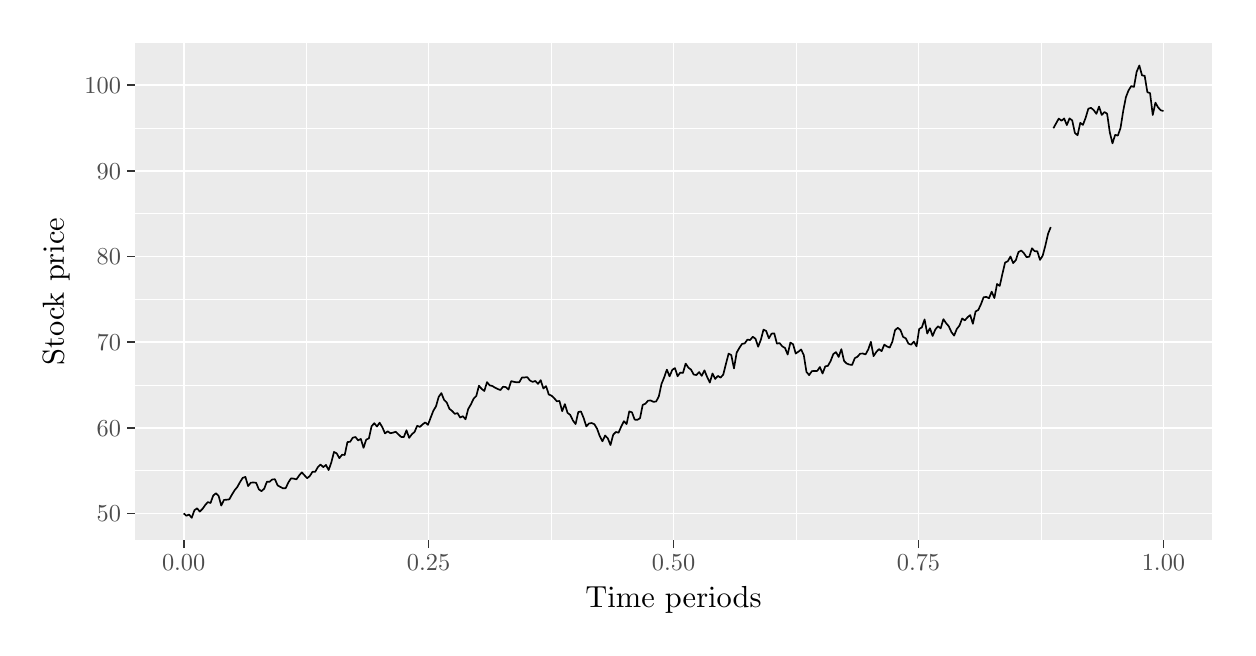
\begin{tikzpicture}[x=1pt,y=1pt]
\definecolor{fillColor}{RGB}{255,255,255}
\path[use as bounding box,fill=fillColor,fill opacity=0.00] (0,0) rectangle (433.62,216.81);
\begin{scope}
\path[clip] (  0.00,  0.00) rectangle (433.62,216.81);
\definecolor{drawColor}{RGB}{255,255,255}
\definecolor{fillColor}{RGB}{255,255,255}

\path[draw=drawColor,line width= 0.6pt,line join=round,line cap=round,fill=fillColor] (  0.00,  0.00) rectangle (433.62,216.81);
\end{scope}
\begin{scope}
\path[clip] ( 38.67, 31.53) rectangle (428.12,211.31);
\definecolor{fillColor}{gray}{0.92}

\path[fill=fillColor] ( 38.67, 31.53) rectangle (428.12,211.31);
\definecolor{drawColor}{RGB}{255,255,255}

\path[draw=drawColor,line width= 0.3pt,line join=round] ( 38.67, 56.77) --
	(428.12, 56.77);

\path[draw=drawColor,line width= 0.3pt,line join=round] ( 38.67, 87.71) --
	(428.12, 87.71);

\path[draw=drawColor,line width= 0.3pt,line join=round] ( 38.67,118.64) --
	(428.12,118.64);

\path[draw=drawColor,line width= 0.3pt,line join=round] ( 38.67,149.58) --
	(428.12,149.58);

\path[draw=drawColor,line width= 0.3pt,line join=round] ( 38.67,180.52) --
	(428.12,180.52);

\path[draw=drawColor,line width= 0.3pt,line join=round] (100.63, 31.53) --
	(100.63,211.31);

\path[draw=drawColor,line width= 0.3pt,line join=round] (189.14, 31.53) --
	(189.14,211.31);

\path[draw=drawColor,line width= 0.3pt,line join=round] (277.65, 31.53) --
	(277.65,211.31);

\path[draw=drawColor,line width= 0.3pt,line join=round] (366.16, 31.53) --
	(366.16,211.31);

\path[draw=drawColor,line width= 0.6pt,line join=round] ( 38.67, 41.30) --
	(428.12, 41.30);

\path[draw=drawColor,line width= 0.6pt,line join=round] ( 38.67, 72.24) --
	(428.12, 72.24);

\path[draw=drawColor,line width= 0.6pt,line join=round] ( 38.67,103.17) --
	(428.12,103.17);

\path[draw=drawColor,line width= 0.6pt,line join=round] ( 38.67,134.11) --
	(428.12,134.11);

\path[draw=drawColor,line width= 0.6pt,line join=round] ( 38.67,165.05) --
	(428.12,165.05);

\path[draw=drawColor,line width= 0.6pt,line join=round] ( 38.67,195.99) --
	(428.12,195.99);

\path[draw=drawColor,line width= 0.6pt,line join=round] ( 56.37, 31.53) --
	( 56.37,211.31);

\path[draw=drawColor,line width= 0.6pt,line join=round] (144.88, 31.53) --
	(144.88,211.31);

\path[draw=drawColor,line width= 0.6pt,line join=round] (233.39, 31.53) --
	(233.39,211.31);

\path[draw=drawColor,line width= 0.6pt,line join=round] (321.91, 31.53) --
	(321.91,211.31);

\path[draw=drawColor,line width= 0.6pt,line join=round] (410.42, 31.53) --
	(410.42,211.31);
\definecolor{drawColor}{RGB}{0,0,0}

\path[draw=drawColor,line width= 0.6pt,line join=round] ( 56.37, 41.30) --
	( 57.34, 40.44) --
	( 58.31, 40.89) --
	( 59.28, 39.70) --
	( 60.25, 42.44) --
	( 61.22, 43.13) --
	( 62.19, 41.95) --
	( 63.16, 42.90) --
	( 64.13, 44.27) --
	( 65.10, 45.39) --
	( 66.07, 45.04) --
	( 67.04, 47.73) --
	( 68.01, 48.55) --
	( 68.98, 47.66) --
	( 69.95, 44.13) --
	( 70.92, 46.15) --
	( 71.89, 46.24) --
	( 72.86, 46.37) --
	( 73.83, 48.12) --
	( 74.80, 49.68) --
	( 75.77, 50.86) --
	( 76.74, 52.62) --
	( 77.71, 54.15) --
	( 78.68, 54.45) --
	( 79.65, 51.16) --
	( 80.62, 52.39) --
	( 81.59, 52.46) --
	( 82.56, 52.36) --
	( 83.53, 49.99) --
	( 84.50, 49.34) --
	( 85.47, 50.22) --
	( 86.44, 52.73) --
	( 87.41, 52.72) --
	( 88.38, 53.56) --
	( 89.35, 53.63) --
	( 90.32, 51.41) --
	( 91.29, 50.86) --
	( 92.26, 50.35) --
	( 93.23, 50.41) --
	( 94.20, 52.47) --
	( 95.17, 53.97) --
	( 96.14, 53.85) --
	( 97.11, 53.58) --
	( 98.08, 54.97) --
	( 99.05, 56.12) --
	(100.02, 55.07) --
	(100.99, 54.00) --
	(101.96, 54.81) --
	(102.93, 56.34) --
	(103.90, 56.31) --
	(104.87, 58.05) --
	(105.84, 58.94) --
	(106.81, 58.01) --
	(107.78, 58.80) --
	(108.75, 56.95) --
	(109.72, 59.70) --
	(110.69, 63.50) --
	(111.66, 63.00) --
	(112.63, 61.26) --
	(113.60, 62.48) --
	(114.57, 62.41) --
	(115.54, 67.06) --
	(116.51, 67.17) --
	(117.48, 68.66) --
	(118.45, 68.90) --
	(119.42, 67.67) --
	(120.39, 68.21) --
	(121.36, 64.99) --
	(122.33, 67.93) --
	(123.30, 68.40) --
	(124.27, 72.77) --
	(125.24, 73.89) --
	(126.21, 72.69) --
	(127.18, 74.07) --
	(128.15, 72.43) --
	(129.12, 70.19) --
	(130.09, 70.94) --
	(131.06, 70.27) --
	(132.03, 70.46) --
	(133.00, 70.79) --
	(133.97, 69.84) --
	(134.94, 68.93) --
	(135.91, 68.86) --
	(136.88, 71.31) --
	(137.85, 68.57) --
	(138.82, 69.89) --
	(139.79, 70.71) --
	(140.76, 72.96) --
	(141.73, 72.55) --
	(142.70, 73.46) --
	(143.67, 74.17) --
	(144.64, 73.30) --
	(145.61, 75.86) --
	(146.58, 78.37) --
	(147.55, 79.97) --
	(148.52, 83.41) --
	(149.49, 84.76) --
	(150.46, 82.33) --
	(151.43, 81.36) --
	(152.40, 79.07) --
	(153.37, 78.31) --
	(154.34, 77.26) --
	(155.31, 77.54) --
	(156.28, 75.91) --
	(157.25, 76.42) --
	(158.22, 75.31) --
	(159.19, 79.03) --
	(160.16, 80.67) --
	(161.13, 82.73) --
	(162.10, 83.72) --
	(163.07, 87.42) --
	(164.04, 86.29) --
	(165.01, 85.53) --
	(165.98, 88.73) --
	(166.95, 87.56) --
	(167.92, 87.33) --
	(168.89, 86.71) --
	(169.86, 86.24) --
	(170.83, 85.86) --
	(171.80, 87.09) --
	(172.77, 86.92) --
	(173.74, 86.06) --
	(174.71, 89.09) --
	(175.68, 88.84) --
	(176.65, 88.66) --
	(177.62, 88.65) --
	(178.59, 90.37) --
	(179.56, 90.42) --
	(180.53, 90.54) --
	(181.50, 89.30) --
	(182.47, 88.81) --
	(183.44, 89.14) --
	(184.41, 88.10) --
	(185.38, 89.43) --
	(186.35, 86.43) --
	(187.32, 87.28) --
	(188.29, 84.27) --
	(189.26, 83.85) --
	(190.23, 82.96) --
	(191.20, 81.82) --
	(192.17, 81.90) --
	(193.14, 78.22) --
	(194.11, 80.79) --
	(195.08, 77.62) --
	(196.05, 76.89) --
	(197.02, 74.87) --
	(197.99, 73.58) --
	(198.96, 77.91) --
	(199.93, 78.13) --
	(200.90, 75.76) --
	(201.87, 72.73) --
	(202.84, 73.79) --
	(203.81, 73.95) --
	(204.78, 73.51) --
	(205.75, 71.89) --
	(206.72, 69.21) --
	(207.69, 67.35) --
	(208.66, 69.43) --
	(209.63, 68.43) --
	(210.60, 65.99) --
	(211.57, 69.72) --
	(212.54, 70.72) --
	(213.51, 70.45) --
	(214.48, 72.69) --
	(215.45, 74.61) --
	(216.42, 73.58) --
	(217.39, 78.14) --
	(218.36, 77.82) --
	(219.33, 75.18) --
	(220.30, 75.09) --
	(221.27, 75.69) --
	(222.24, 80.51) --
	(223.21, 80.92) --
	(224.18, 82.04) --
	(225.15, 82.08) --
	(226.12, 81.60) --
	(227.09, 81.72) --
	(228.06, 83.54) --
	(229.03, 88.06) --
	(230.00, 90.45) --
	(230.97, 93.25) --
	(231.94, 90.81) --
	(232.91, 93.13) --
	(233.88, 93.81) --
	(234.85, 90.86) --
	(235.82, 92.18) --
	(236.79, 92.05) --
	(237.76, 95.43) --
	(238.73, 93.97) --
	(239.70, 93.25) --
	(240.67, 91.46) --
	(241.64, 91.29) --
	(242.61, 92.36) --
	(243.58, 90.99) --
	(244.55, 92.98) --
	(245.52, 90.59) --
	(246.49, 88.57) --
	(247.46, 91.85) --
	(248.43, 89.88) --
	(249.40, 90.97) --
	(250.37, 90.36) --
	(251.34, 91.44) --
	(252.31, 95.30) --
	(253.28, 99.01) --
	(254.25, 98.49) --
	(255.22, 93.69) --
	(256.19, 99.39) --
	(257.16,101.09) --
	(258.13,102.53) --
	(259.10,102.72) --
	(260.07,104.09) --
	(261.04,103.94) --
	(262.01,105.11) --
	(262.98,104.42) --
	(263.95,101.53) --
	(264.92,103.99) --
	(265.89,107.69) --
	(266.86,107.20) --
	(267.83,104.55) --
	(268.80,106.24) --
	(269.77,106.36) --
	(270.74,102.62) --
	(271.71,102.84) --
	(272.68,101.64) --
	(273.65,101.09) --
	(274.62, 98.72) --
	(275.59,102.98) --
	(276.56,102.45) --
	(277.53, 99.06) --
	(278.50, 99.72) --
	(279.47,100.52) --
	(280.44, 98.53) --
	(281.41, 92.43) --
	(282.38, 91.26) --
	(283.35, 92.69) --
	(284.32, 92.77) --
	(285.29, 92.77) --
	(286.26, 94.19) --
	(287.23, 91.83) --
	(288.20, 94.41) --
	(289.17, 94.61) --
	(290.14, 96.36) --
	(291.11, 98.86) --
	(292.08, 99.57) --
	(293.05, 97.83) --
	(294.02,100.64) --
	(294.99, 96.41) --
	(295.96, 95.43) --
	(296.93, 95.08) --
	(297.90, 94.93) --
	(298.87, 97.38) --
	(299.84, 97.89) --
	(300.81, 99.01) --
	(301.78, 99.06) --
	(302.75, 98.73) --
	(303.72,100.49) --
	(304.69,103.29) --
	(305.66, 98.12) --
	(306.63, 99.61) --
	(307.60,100.66) --
	(308.57, 99.92) --
	(309.54,102.27) --
	(310.51,101.61) --
	(311.48,101.19) --
	(312.45,103.34) --
	(313.42,107.50) --
	(314.39,108.35) --
	(315.36,107.59) --
	(316.33,105.08) --
	(317.30,104.54) --
	(318.27,102.63) --
	(319.24,102.26) --
	(320.21,103.37) --
	(321.18,101.66) --
	(322.15,107.93) --
	(323.12,108.51) --
	(324.09,111.38) --
	(325.06,106.28) --
	(326.03,108.21) --
	(327.00,105.40) --
	(327.97,107.74) --
	(328.94,108.89) --
	(329.91,108.16) --
	(330.88,111.48) --
	(331.85,110.06) --
	(332.82,108.93) --
	(333.79,106.83) --
	(334.76,105.52) --
	(335.73,107.92) --
	(336.70,109.15) --
	(337.67,111.73) --
	(338.64,111.04) --
	(339.61,112.15) --
	(340.58,112.95) --
	(341.55,109.82) --
	(342.52,114.25) --
	(343.49,114.80) --
	(344.46,116.86) --
	(345.43,119.41) --
	(346.40,119.52) --
	(347.37,119.01) --
	(348.34,121.43) --
	(349.31,119.10) --
	(350.28,124.19) --
	(351.25,123.48) --
	(352.22,127.86) --
	(353.19,131.95) --
	(354.16,132.41) --
	(355.13,134.13) --
	(356.10,131.73) --
	(357.07,132.81) --
	(358.04,135.76) --
	(359.01,136.27) --
	(359.98,135.34) --
	(360.95,133.89) --
	(361.92,134.04) --
	(362.89,137.08) --
	(363.86,136.06) --
	(364.83,136.00) --
	(365.80,132.89) --
	(366.77,134.42) --
	(367.74,138.09) --
	(368.71,142.31) --
	(369.68,144.76);

\path[draw=drawColor,line width= 0.6pt,line join=round] (370.65,180.47) --
	(371.62,182.25) --
	(372.59,183.97) --
	(373.56,183.17) --
	(374.53,184.00) --
	(375.50,181.61) --
	(376.47,184.02) --
	(377.44,183.30) --
	(378.41,178.76) --
	(379.38,177.93) --
	(380.35,182.42) --
	(381.32,181.68) --
	(382.29,184.25) --
	(383.26,187.52) --
	(384.23,187.84) --
	(385.20,187.03) --
	(386.17,185.67) --
	(387.14,188.30) --
	(388.11,185.26) --
	(389.08,186.33) --
	(390.05,185.72) --
	(391.02,179.01) --
	(391.99,175.01) --
	(392.96,178.09) --
	(393.93,177.80) --
	(394.90,180.55) --
	(395.87,186.72) --
	(396.84,191.69) --
	(397.81,194.17) --
	(398.78,195.71) --
	(399.75,195.39) --
	(400.72,200.85) --
	(401.69,203.14) --
	(402.66,199.59) --
	(403.63,199.39) --
	(404.60,193.48) --
	(405.57,193.16) --
	(406.54,185.25) --
	(407.51,189.70) --
	(408.48,187.99) --
	(409.45,186.94) --
	(410.42,186.71);
\end{scope}
\begin{scope}
\path[clip] (  0.00,  0.00) rectangle (433.62,216.81);
\definecolor{drawColor}{gray}{0.30}

\node[text=drawColor,anchor=base east,inner sep=0pt, outer sep=0pt, scale=  0.88] at ( 33.72, 38.27) {50};

\node[text=drawColor,anchor=base east,inner sep=0pt, outer sep=0pt, scale=  0.88] at ( 33.72, 69.21) {60};

\node[text=drawColor,anchor=base east,inner sep=0pt, outer sep=0pt, scale=  0.88] at ( 33.72,100.14) {70};

\node[text=drawColor,anchor=base east,inner sep=0pt, outer sep=0pt, scale=  0.88] at ( 33.72,131.08) {80};

\node[text=drawColor,anchor=base east,inner sep=0pt, outer sep=0pt, scale=  0.88] at ( 33.72,162.02) {90};

\node[text=drawColor,anchor=base east,inner sep=0pt, outer sep=0pt, scale=  0.88] at ( 33.72,192.96) {100};
\end{scope}
\begin{scope}
\path[clip] (  0.00,  0.00) rectangle (433.62,216.81);
\definecolor{drawColor}{gray}{0.20}

\path[draw=drawColor,line width= 0.6pt,line join=round] ( 35.92, 41.30) --
	( 38.67, 41.30);

\path[draw=drawColor,line width= 0.6pt,line join=round] ( 35.92, 72.24) --
	( 38.67, 72.24);

\path[draw=drawColor,line width= 0.6pt,line join=round] ( 35.92,103.17) --
	( 38.67,103.17);

\path[draw=drawColor,line width= 0.6pt,line join=round] ( 35.92,134.11) --
	( 38.67,134.11);

\path[draw=drawColor,line width= 0.6pt,line join=round] ( 35.92,165.05) --
	( 38.67,165.05);

\path[draw=drawColor,line width= 0.6pt,line join=round] ( 35.92,195.99) --
	( 38.67,195.99);
\end{scope}
\begin{scope}
\path[clip] (  0.00,  0.00) rectangle (433.62,216.81);
\definecolor{drawColor}{gray}{0.20}

\path[draw=drawColor,line width= 0.6pt,line join=round] ( 56.37, 28.78) --
	( 56.37, 31.53);

\path[draw=drawColor,line width= 0.6pt,line join=round] (144.88, 28.78) --
	(144.88, 31.53);

\path[draw=drawColor,line width= 0.6pt,line join=round] (233.39, 28.78) --
	(233.39, 31.53);

\path[draw=drawColor,line width= 0.6pt,line join=round] (321.91, 28.78) --
	(321.91, 31.53);

\path[draw=drawColor,line width= 0.6pt,line join=round] (410.42, 28.78) --
	(410.42, 31.53);
\end{scope}
\begin{scope}
\path[clip] (  0.00,  0.00) rectangle (433.62,216.81);
\definecolor{drawColor}{gray}{0.30}

\node[text=drawColor,anchor=base,inner sep=0pt, outer sep=0pt, scale=  0.88] at ( 56.37, 20.52) {0.00};

\node[text=drawColor,anchor=base,inner sep=0pt, outer sep=0pt, scale=  0.88] at (144.88, 20.52) {0.25};

\node[text=drawColor,anchor=base,inner sep=0pt, outer sep=0pt, scale=  0.88] at (233.39, 20.52) {0.50};

\node[text=drawColor,anchor=base,inner sep=0pt, outer sep=0pt, scale=  0.88] at (321.91, 20.52) {0.75};

\node[text=drawColor,anchor=base,inner sep=0pt, outer sep=0pt, scale=  0.88] at (410.42, 20.52) {1.00};
\end{scope}
\begin{scope}
\path[clip] (  0.00,  0.00) rectangle (433.62,216.81);
\definecolor{drawColor}{RGB}{0,0,0}

\node[text=drawColor,anchor=base,inner sep=0pt, outer sep=0pt, scale=  1.10] at (233.39,  7.44) {Time periods};
\end{scope}
\begin{scope}
\path[clip] (  0.00,  0.00) rectangle (433.62,216.81);
\definecolor{drawColor}{RGB}{0,0,0}

\node[text=drawColor,rotate= 90.00,anchor=base,inner sep=0pt, outer sep=0pt, scale=  1.10] at ( 13.08,121.42) {Stock price};
\end{scope}
\end{tikzpicture}
 
  \floatfoot{Simulation of one Merton mixed jump-diffusion time serie. Data have been output by the R function \textit{sstoch\_jump()} which is an implementation of equation \cref{eq:other:merton:pde} (see appendix \ref{sub:r:time:merton}, for more information). The parameters passed to the function are:  $S(0) = 50$,   $T = 1$ (in year, along with a time step of 365 measures per year),  $\sigma = 0.2$, $\alpha = 0.5$,  $\lambda = 2$,  $\mu = 0.05$, and $\delta = 0.1$.}
  \caption{Merton mixed jump-diffusion time serie}
  \label{p:other:merton:path}
\end{figure}




%%%%%%%%%%%%%%%%%%%%%%%%%%%%%%%%%%%%%%%%%%%%%%%%
% SUBSECTION: Skewness
%%%%%%%%%%%%%%%%%%%%%%%%%%%%%%%%%%%%%%%%%%%%%%%%
\subsection{Impact on the skewness log--return}
\label{sub:MertonSkewness}

The way to influence the direction of the distibution's shape is achieved by moving the cursor of the expected value of jump impact, in other word, by changing the value of the parameter $\mu$. The figure [REF] shows how the density's shape of the log--return may vary along with this parameter.


\begin{figure}[ht]
\centering
% Created by tikzDevice version 0.11 on 2018-04-10 23:12:32
% !TEX encoding = UTF-8 Unicode
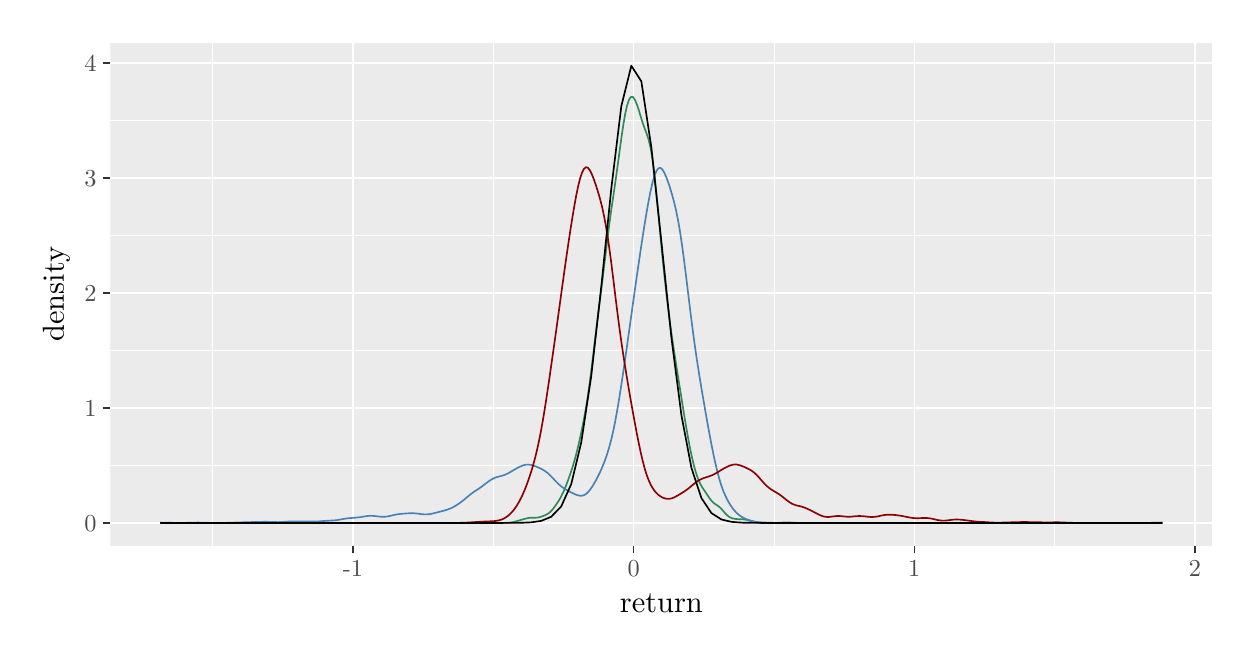
\begin{tikzpicture}[x=1pt,y=1pt]
\definecolor{fillColor}{RGB}{255,255,255}
\path[use as bounding box,fill=fillColor,fill opacity=0.00] (0,0) rectangle (433.62,216.81);
\begin{scope}
\path[clip] (  0.00,  0.00) rectangle (433.62,216.81);
\definecolor{drawColor}{RGB}{255,255,255}
\definecolor{fillColor}{RGB}{255,255,255}

\path[draw=drawColor,line width= 0.6pt,line join=round,line cap=round,fill=fillColor] (  0.00,  0.00) rectangle (433.62,216.81);
\end{scope}
\begin{scope}
\path[clip] ( 29.87, 29.59) rectangle (428.12,211.31);
\definecolor{fillColor}{gray}{0.92}

\path[fill=fillColor] ( 29.87, 29.59) rectangle (428.12,211.31);
\definecolor{drawColor}{RGB}{255,255,255}

\path[draw=drawColor,line width= 0.3pt,line join=round] ( 29.87, 58.62) --
	(428.12, 58.62);

\path[draw=drawColor,line width= 0.3pt,line join=round] ( 29.87,100.17) --
	(428.12,100.17);

\path[draw=drawColor,line width= 0.3pt,line join=round] ( 29.87,141.71) --
	(428.12,141.71);

\path[draw=drawColor,line width= 0.3pt,line join=round] ( 29.87,183.26) --
	(428.12,183.26);

\path[draw=drawColor,line width= 0.3pt,line join=round] ( 66.80, 29.59) --
	( 66.80,211.31);

\path[draw=drawColor,line width= 0.3pt,line join=round] (168.24, 29.59) --
	(168.24,211.31);

\path[draw=drawColor,line width= 0.3pt,line join=round] (269.68, 29.59) --
	(269.68,211.31);

\path[draw=drawColor,line width= 0.3pt,line join=round] (371.11, 29.59) --
	(371.11,211.31);

\path[draw=drawColor,line width= 0.6pt,line join=round] ( 29.87, 37.85) --
	(428.12, 37.85);

\path[draw=drawColor,line width= 0.6pt,line join=round] ( 29.87, 79.39) --
	(428.12, 79.39);

\path[draw=drawColor,line width= 0.6pt,line join=round] ( 29.87,120.94) --
	(428.12,120.94);

\path[draw=drawColor,line width= 0.6pt,line join=round] ( 29.87,162.49) --
	(428.12,162.49);

\path[draw=drawColor,line width= 0.6pt,line join=round] ( 29.87,204.03) --
	(428.12,204.03);

\path[draw=drawColor,line width= 0.6pt,line join=round] (117.52, 29.59) --
	(117.52,211.31);

\path[draw=drawColor,line width= 0.6pt,line join=round] (218.96, 29.59) --
	(218.96,211.31);

\path[draw=drawColor,line width= 0.6pt,line join=round] (320.39, 29.59) --
	(320.39,211.31);

\path[draw=drawColor,line width= 0.6pt,line join=round] (421.83, 29.59) --
	(421.83,211.31);
\definecolor{drawColor}{RGB}{46,139,87}

\path[draw=drawColor,line width= 0.6pt,line join=round] ( 47.97, 37.85) --
	( 48.68, 37.85) --
	( 49.39, 37.85) --
	( 50.10, 37.85) --
	( 50.81, 37.85) --
	( 51.51, 37.85) --
	( 52.22, 37.85) --
	( 52.93, 37.85) --
	( 53.64, 37.85) --
	( 54.35, 37.85) --
	( 55.06, 37.85) --
	( 55.76, 37.85) --
	( 56.47, 37.85) --
	( 57.18, 37.85) --
	( 57.89, 37.85) --
	( 58.60, 37.85) --
	( 59.31, 37.85) --
	( 60.02, 37.85) --
	( 60.72, 37.85) --
	( 61.43, 37.85) --
	( 62.14, 37.85) --
	( 62.85, 37.85) --
	( 63.56, 37.85) --
	( 64.27, 37.85) --
	( 64.98, 37.85) --
	( 65.68, 37.85) --
	( 66.39, 37.85) --
	( 67.10, 37.85) --
	( 67.81, 37.85) --
	( 68.52, 37.85) --
	( 69.23, 37.85) --
	( 69.93, 37.85) --
	( 70.64, 37.85) --
	( 71.35, 37.85) --
	( 72.06, 37.85) --
	( 72.77, 37.85) --
	( 73.48, 37.85) --
	( 74.19, 37.85) --
	( 74.89, 37.85) --
	( 75.60, 37.85) --
	( 76.31, 37.85) --
	( 77.02, 37.85) --
	( 77.73, 37.85) --
	( 78.44, 37.85) --
	( 79.15, 37.85) --
	( 79.85, 37.85) --
	( 80.56, 37.85) --
	( 81.27, 37.85) --
	( 81.98, 37.85) --
	( 82.69, 37.85) --
	( 83.40, 37.85) --
	( 84.10, 37.85) --
	( 84.81, 37.85) --
	( 85.52, 37.85) --
	( 86.23, 37.85) --
	( 86.94, 37.85) --
	( 87.65, 37.85) --
	( 88.36, 37.85) --
	( 89.06, 37.85) --
	( 89.77, 37.85) --
	( 90.48, 37.85) --
	( 91.19, 37.85) --
	( 91.90, 37.85) --
	( 92.61, 37.85) --
	( 93.32, 37.85) --
	( 94.02, 37.85) --
	( 94.73, 37.85) --
	( 95.44, 37.85) --
	( 96.15, 37.85) --
	( 96.86, 37.85) --
	( 97.57, 37.85) --
	( 98.28, 37.85) --
	( 98.98, 37.85) --
	( 99.69, 37.85) --
	(100.40, 37.85) --
	(101.11, 37.85) --
	(101.82, 37.85) --
	(102.53, 37.85) --
	(103.23, 37.85) --
	(103.94, 37.85) --
	(104.65, 37.85) --
	(105.36, 37.85) --
	(106.07, 37.85) --
	(106.78, 37.85) --
	(107.49, 37.85) --
	(108.19, 37.85) --
	(108.90, 37.85) --
	(109.61, 37.85) --
	(110.32, 37.85) --
	(111.03, 37.85) --
	(111.74, 37.85) --
	(112.45, 37.85) --
	(113.15, 37.85) --
	(113.86, 37.85) --
	(114.57, 37.85) --
	(115.28, 37.85) --
	(115.99, 37.85) --
	(116.70, 37.85) --
	(117.40, 37.85) --
	(118.11, 37.85) --
	(118.82, 37.85) --
	(119.53, 37.85) --
	(120.24, 37.85) --
	(120.95, 37.85) --
	(121.66, 37.85) --
	(122.36, 37.85) --
	(123.07, 37.85) --
	(123.78, 37.85) --
	(124.49, 37.85) --
	(125.20, 37.85) --
	(125.91, 37.85) --
	(126.62, 37.85) --
	(127.32, 37.85) --
	(128.03, 37.85) --
	(128.74, 37.85) --
	(129.45, 37.85) --
	(130.16, 37.85) --
	(130.87, 37.85) --
	(131.57, 37.85) --
	(132.28, 37.85) --
	(132.99, 37.85) --
	(133.70, 37.85) --
	(134.41, 37.85) --
	(135.12, 37.85) --
	(135.83, 37.85) --
	(136.53, 37.85) --
	(137.24, 37.85) --
	(137.95, 37.85) --
	(138.66, 37.85) --
	(139.37, 37.85) --
	(140.08, 37.85) --
	(140.79, 37.85) --
	(141.49, 37.85) --
	(142.20, 37.85) --
	(142.91, 37.85) --
	(143.62, 37.85) --
	(144.33, 37.85) --
	(145.04, 37.85) --
	(145.74, 37.85) --
	(146.45, 37.85) --
	(147.16, 37.85) --
	(147.87, 37.85) --
	(148.58, 37.85) --
	(149.29, 37.85) --
	(150.00, 37.85) --
	(150.70, 37.85) --
	(151.41, 37.85) --
	(152.12, 37.85) --
	(152.83, 37.85) --
	(153.54, 37.85) --
	(154.25, 37.85) --
	(154.96, 37.85) --
	(155.66, 37.85) --
	(156.37, 37.85) --
	(157.08, 37.85) --
	(157.79, 37.85) --
	(158.50, 37.86) --
	(159.21, 37.87) --
	(159.92, 37.89) --
	(160.62, 37.93) --
	(161.33, 37.97) --
	(162.04, 38.01) --
	(162.75, 38.03) --
	(163.46, 38.02) --
	(164.17, 38.00) --
	(164.87, 37.96) --
	(165.58, 37.92) --
	(166.29, 37.88) --
	(167.00, 37.86) --
	(167.71, 37.85) --
	(168.42, 37.85) --
	(169.13, 37.85) --
	(169.83, 37.85) --
	(170.54, 37.85) --
	(171.25, 37.85) --
	(171.96, 37.85) --
	(172.67, 37.87) --
	(173.38, 37.89) --
	(174.09, 37.95) --
	(174.79, 38.04) --
	(175.50, 38.18) --
	(176.21, 38.35) --
	(176.92, 38.55) --
	(177.63, 38.76) --
	(178.34, 38.97) --
	(179.04, 39.16) --
	(179.75, 39.35) --
	(180.46, 39.53) --
	(181.17, 39.67) --
	(181.88, 39.74) --
	(182.59, 39.74) --
	(183.30, 39.73) --
	(184.00, 39.76) --
	(184.71, 39.87) --
	(185.42, 40.06) --
	(186.13, 40.31) --
	(186.84, 40.59) --
	(187.55, 40.92) --
	(188.26, 41.35) --
	(188.96, 41.95) --
	(189.67, 42.72) --
	(190.38, 43.64) --
	(191.09, 44.65) --
	(191.80, 45.73) --
	(192.51, 46.92) --
	(193.21, 48.27) --
	(193.92, 49.81) --
	(194.63, 51.56) --
	(195.34, 53.46) --
	(196.05, 55.49) --
	(196.76, 57.64) --
	(197.47, 59.97) --
	(198.17, 62.53) --
	(198.88, 65.35) --
	(199.59, 68.45) --
	(200.30, 71.81) --
	(201.01, 75.44) --
	(201.72, 79.40) --
	(202.43, 83.82) --
	(203.13, 88.81) --
	(203.84, 94.36) --
	(204.55,100.28) --
	(205.26,106.28) --
	(205.97,112.07) --
	(206.68,117.64) --
	(207.39,123.17) --
	(208.09,128.86) --
	(208.80,134.75) --
	(209.51,140.63) --
	(210.22,146.18) --
	(210.93,151.28) --
	(211.64,156.10) --
	(212.34,160.94) --
	(213.05,166.00) --
	(213.76,171.26) --
	(214.47,176.49) --
	(215.18,181.37) --
	(215.89,185.54) --
	(216.60,188.75) --
	(217.30,190.84) --
	(218.01,191.81) --
	(218.72,191.74) --
	(219.43,190.77) --
	(220.14,189.08) --
	(220.85,186.92) --
	(221.56,184.56) --
	(222.26,182.32) --
	(222.97,180.34) --
	(223.68,178.49) --
	(224.39,176.31) --
	(225.10,173.28) --
	(225.81,168.97) --
	(226.51,163.33) --
	(227.22,156.61) --
	(227.93,149.23) --
	(228.64,141.66) --
	(229.35,134.28) --
	(230.06,127.33) --
	(230.77,120.90) --
	(231.47,114.98) --
	(232.18,109.53) --
	(232.89,104.47) --
	(233.60, 99.71) --
	(234.31, 95.15) --
	(235.02, 90.69) --
	(235.73, 86.25) --
	(236.43, 81.81) --
	(237.14, 77.38) --
	(237.85, 73.08) --
	(238.56, 69.00) --
	(239.27, 65.24) --
	(239.98, 61.85) --
	(240.68, 58.86) --
	(241.39, 56.28) --
	(242.10, 54.14) --
	(242.81, 52.43) --
	(243.52, 51.09) --
	(244.23, 49.97) --
	(244.94, 48.94) --
	(245.64, 47.88) --
	(246.35, 46.83) --
	(247.06, 45.89) --
	(247.77, 45.16) --
	(248.48, 44.63) --
	(249.19, 44.18) --
	(249.90, 43.66) --
	(250.60, 42.98) --
	(251.31, 42.18) --
	(252.02, 41.36) --
	(252.73, 40.64) --
	(253.44, 40.08) --
	(254.15, 39.69) --
	(254.85, 39.46) --
	(255.56, 39.32) --
	(256.27, 39.24) --
	(256.98, 39.20) --
	(257.69, 39.18) --
	(258.40, 39.16) --
	(259.11, 39.09) --
	(259.81, 38.96) --
	(260.52, 38.76) --
	(261.23, 38.54) --
	(261.94, 38.31) --
	(262.65, 38.13) --
	(263.36, 38.00) --
	(264.07, 37.92) --
	(264.77, 37.88) --
	(265.48, 37.86) --
	(266.19, 37.85) --
	(266.90, 37.85) --
	(267.61, 37.85) --
	(268.32, 37.85) --
	(269.03, 37.85) --
	(269.73, 37.85) --
	(270.44, 37.87) --
	(271.15, 37.89) --
	(271.86, 37.92) --
	(272.57, 37.96) --
	(273.28, 38.00) --
	(273.98, 38.03) --
	(274.69, 38.03) --
	(275.40, 38.00) --
	(276.11, 37.96) --
	(276.82, 37.92) --
	(277.53, 37.89) --
	(278.24, 37.87) --
	(278.94, 37.85) --
	(279.65, 37.85) --
	(280.36, 37.85) --
	(281.07, 37.85) --
	(281.78, 37.85) --
	(282.49, 37.85) --
	(283.20, 37.85) --
	(283.90, 37.85) --
	(284.61, 37.85) --
	(285.32, 37.85) --
	(286.03, 37.85) --
	(286.74, 37.85) --
	(287.45, 37.85) --
	(288.15, 37.85) --
	(288.86, 37.85) --
	(289.57, 37.85) --
	(290.28, 37.85) --
	(290.99, 37.85) --
	(291.70, 37.85) --
	(292.41, 37.85) --
	(293.11, 37.85) --
	(293.82, 37.85) --
	(294.53, 37.85) --
	(295.24, 37.85) --
	(295.95, 37.85) --
	(296.66, 37.85) --
	(297.37, 37.85) --
	(298.07, 37.85) --
	(298.78, 37.85) --
	(299.49, 37.85) --
	(300.20, 37.85) --
	(300.91, 37.85) --
	(301.62, 37.85) --
	(302.32, 37.85) --
	(303.03, 37.85) --
	(303.74, 37.85) --
	(304.45, 37.85) --
	(305.16, 37.85) --
	(305.87, 37.85) --
	(306.58, 37.85) --
	(307.28, 37.85) --
	(307.99, 37.85) --
	(308.70, 37.85) --
	(309.41, 37.85) --
	(310.12, 37.85) --
	(310.83, 37.85) --
	(311.54, 37.85) --
	(312.24, 37.85) --
	(312.95, 37.85) --
	(313.66, 37.85) --
	(314.37, 37.85) --
	(315.08, 37.85) --
	(315.79, 37.85) --
	(316.49, 37.85) --
	(317.20, 37.85) --
	(317.91, 37.85) --
	(318.62, 37.85) --
	(319.33, 37.85) --
	(320.04, 37.85) --
	(320.75, 37.85) --
	(321.45, 37.85) --
	(322.16, 37.85) --
	(322.87, 37.85) --
	(323.58, 37.85) --
	(324.29, 37.85) --
	(325.00, 37.85) --
	(325.71, 37.85) --
	(326.41, 37.85) --
	(327.12, 37.85) --
	(327.83, 37.85) --
	(328.54, 37.85) --
	(329.25, 37.85) --
	(329.96, 37.85) --
	(330.67, 37.85) --
	(331.37, 37.85) --
	(332.08, 37.85) --
	(332.79, 37.85) --
	(333.50, 37.85) --
	(334.21, 37.85) --
	(334.92, 37.85) --
	(335.62, 37.85) --
	(336.33, 37.85) --
	(337.04, 37.85) --
	(337.75, 37.85) --
	(338.46, 37.85) --
	(339.17, 37.85) --
	(339.88, 37.85) --
	(340.58, 37.85) --
	(341.29, 37.85) --
	(342.00, 37.85) --
	(342.71, 37.85) --
	(343.42, 37.85) --
	(344.13, 37.85) --
	(344.84, 37.85) --
	(345.54, 37.85) --
	(346.25, 37.85) --
	(346.96, 37.85) --
	(347.67, 37.85) --
	(348.38, 37.85) --
	(349.09, 37.85) --
	(349.79, 37.85) --
	(350.50, 37.85) --
	(351.21, 37.85) --
	(351.92, 37.85) --
	(352.63, 37.85) --
	(353.34, 37.85) --
	(354.05, 37.85) --
	(354.75, 37.85) --
	(355.46, 37.85) --
	(356.17, 37.85) --
	(356.88, 37.85) --
	(357.59, 37.85) --
	(358.30, 37.85) --
	(359.01, 37.85) --
	(359.71, 37.85) --
	(360.42, 37.85) --
	(361.13, 37.85) --
	(361.84, 37.85) --
	(362.55, 37.85) --
	(363.26, 37.85) --
	(363.96, 37.85) --
	(364.67, 37.85) --
	(365.38, 37.85) --
	(366.09, 37.85) --
	(366.80, 37.85) --
	(367.51, 37.85) --
	(368.22, 37.85) --
	(368.92, 37.85) --
	(369.63, 37.85) --
	(370.34, 37.85) --
	(371.05, 37.85) --
	(371.76, 37.85) --
	(372.47, 37.85) --
	(373.18, 37.85) --
	(373.88, 37.85) --
	(374.59, 37.85) --
	(375.30, 37.85) --
	(376.01, 37.85) --
	(376.72, 37.85) --
	(377.43, 37.85) --
	(378.13, 37.85) --
	(378.84, 37.85) --
	(379.55, 37.85) --
	(380.26, 37.85) --
	(380.97, 37.85) --
	(381.68, 37.85) --
	(382.39, 37.85) --
	(383.09, 37.85) --
	(383.80, 37.85) --
	(384.51, 37.85) --
	(385.22, 37.85) --
	(385.93, 37.85) --
	(386.64, 37.85) --
	(387.35, 37.85) --
	(388.05, 37.85) --
	(388.76, 37.85) --
	(389.47, 37.85) --
	(390.18, 37.85) --
	(390.89, 37.85) --
	(391.60, 37.85) --
	(392.31, 37.85) --
	(393.01, 37.85) --
	(393.72, 37.85) --
	(394.43, 37.85) --
	(395.14, 37.85) --
	(395.85, 37.85) --
	(396.56, 37.85) --
	(397.26, 37.85) --
	(397.97, 37.85) --
	(398.68, 37.85) --
	(399.39, 37.85) --
	(400.10, 37.85) --
	(400.81, 37.85) --
	(401.52, 37.85) --
	(402.22, 37.85) --
	(402.93, 37.85) --
	(403.64, 37.85) --
	(404.35, 37.85) --
	(405.06, 37.85) --
	(405.77, 37.85) --
	(406.48, 37.85) --
	(407.18, 37.85) --
	(407.89, 37.85) --
	(408.60, 37.85) --
	(409.31, 37.85) --
	(410.02, 37.85);
\definecolor{drawColor}{RGB}{70,130,180}

\path[draw=drawColor,line width= 0.6pt,line join=round] ( 47.97, 37.98) --
	( 48.68, 37.97) --
	( 49.39, 37.96) --
	( 50.10, 37.94) --
	( 50.81, 37.92) --
	( 51.51, 37.90) --
	( 52.22, 37.88) --
	( 52.93, 37.87) --
	( 53.64, 37.86) --
	( 54.35, 37.86) --
	( 55.06, 37.86) --
	( 55.76, 37.86) --
	( 56.47, 37.87) --
	( 57.18, 37.88) --
	( 57.89, 37.90) --
	( 58.60, 37.91) --
	( 59.31, 37.94) --
	( 60.02, 37.96) --
	( 60.72, 37.97) --
	( 61.43, 37.98) --
	( 62.14, 37.97) --
	( 62.85, 37.96) --
	( 63.56, 37.94) --
	( 64.27, 37.92) --
	( 64.98, 37.90) --
	( 65.68, 37.88) --
	( 66.39, 37.87) --
	( 67.10, 37.86) --
	( 67.81, 37.86) --
	( 68.52, 37.85) --
	( 69.23, 37.85) --
	( 69.93, 37.86) --
	( 70.64, 37.86) --
	( 71.35, 37.87) --
	( 72.06, 37.89) --
	( 72.77, 37.91) --
	( 73.48, 37.93) --
	( 74.19, 37.96) --
	( 74.89, 37.98) --
	( 75.60, 38.01) --
	( 76.31, 38.03) --
	( 77.02, 38.05) --
	( 77.73, 38.07) --
	( 78.44, 38.09) --
	( 79.15, 38.12) --
	( 79.85, 38.14) --
	( 80.56, 38.15) --
	( 81.27, 38.17) --
	( 81.98, 38.18) --
	( 82.69, 38.19) --
	( 83.40, 38.20) --
	( 84.10, 38.22) --
	( 84.81, 38.24) --
	( 85.52, 38.26) --
	( 86.23, 38.26) --
	( 86.94, 38.25) --
	( 87.65, 38.23) --
	( 88.36, 38.20) --
	( 89.06, 38.18) --
	( 89.77, 38.16) --
	( 90.48, 38.15) --
	( 91.19, 38.17) --
	( 91.90, 38.20) --
	( 92.61, 38.24) --
	( 93.32, 38.29) --
	( 94.02, 38.33) --
	( 94.73, 38.36) --
	( 95.44, 38.38) --
	( 96.15, 38.39) --
	( 96.86, 38.39) --
	( 97.57, 38.39) --
	( 98.28, 38.40) --
	( 98.98, 38.40) --
	( 99.69, 38.41) --
	(100.40, 38.40) --
	(101.11, 38.39) --
	(101.82, 38.38) --
	(102.53, 38.37) --
	(103.23, 38.36) --
	(103.94, 38.36) --
	(104.65, 38.38) --
	(105.36, 38.42) --
	(106.07, 38.47) --
	(106.78, 38.53) --
	(107.49, 38.58) --
	(108.19, 38.63) --
	(108.90, 38.67) --
	(109.61, 38.70) --
	(110.32, 38.74) --
	(111.03, 38.80) --
	(111.74, 38.88) --
	(112.45, 38.99) --
	(113.15, 39.11) --
	(113.86, 39.24) --
	(114.57, 39.37) --
	(115.28, 39.47) --
	(115.99, 39.56) --
	(116.70, 39.62) --
	(117.40, 39.67) --
	(118.11, 39.72) --
	(118.82, 39.78) --
	(119.53, 39.86) --
	(120.24, 39.95) --
	(120.95, 40.07) --
	(121.66, 40.19) --
	(122.36, 40.30) --
	(123.07, 40.38) --
	(123.78, 40.42) --
	(124.49, 40.41) --
	(125.20, 40.36) --
	(125.91, 40.28) --
	(126.62, 40.19) --
	(127.32, 40.12) --
	(128.03, 40.07) --
	(128.74, 40.07) --
	(129.45, 40.12) --
	(130.16, 40.23) --
	(130.87, 40.37) --
	(131.57, 40.54) --
	(132.28, 40.70) --
	(132.99, 40.86) --
	(133.70, 40.98) --
	(134.41, 41.07) --
	(135.12, 41.14) --
	(135.83, 41.20) --
	(136.53, 41.25) --
	(137.24, 41.30) --
	(137.95, 41.34) --
	(138.66, 41.36) --
	(139.37, 41.34) --
	(140.08, 41.30) --
	(140.79, 41.23) --
	(141.49, 41.14) --
	(142.20, 41.04) --
	(142.91, 40.97) --
	(143.62, 40.93) --
	(144.33, 40.95) --
	(145.04, 41.01) --
	(145.74, 41.12) --
	(146.45, 41.27) --
	(147.16, 41.45) --
	(147.87, 41.63) --
	(148.58, 41.82) --
	(149.29, 42.00) --
	(150.00, 42.18) --
	(150.70, 42.37) --
	(151.41, 42.58) --
	(152.12, 42.83) --
	(152.83, 43.11) --
	(153.54, 43.45) --
	(154.25, 43.83) --
	(154.96, 44.25) --
	(155.66, 44.72) --
	(156.37, 45.22) --
	(157.08, 45.76) --
	(157.79, 46.33) --
	(158.50, 46.92) --
	(159.21, 47.51) --
	(159.92, 48.09) --
	(160.62, 48.63) --
	(161.33, 49.13) --
	(162.04, 49.60) --
	(162.75, 50.06) --
	(163.46, 50.54) --
	(164.17, 51.05) --
	(164.87, 51.59) --
	(165.58, 52.14) --
	(166.29, 52.67) --
	(167.00, 53.17) --
	(167.71, 53.60) --
	(168.42, 53.96) --
	(169.13, 54.25) --
	(169.83, 54.48) --
	(170.54, 54.68) --
	(171.25, 54.87) --
	(171.96, 55.08) --
	(172.67, 55.35) --
	(173.38, 55.67) --
	(174.09, 56.05) --
	(174.79, 56.46) --
	(175.50, 56.88) --
	(176.21, 57.29) --
	(176.92, 57.69) --
	(177.63, 58.06) --
	(178.34, 58.38) --
	(179.04, 58.65) --
	(179.75, 58.84) --
	(180.46, 58.93) --
	(181.17, 58.92) --
	(181.88, 58.81) --
	(182.59, 58.63) --
	(183.30, 58.38) --
	(184.00, 58.11) --
	(184.71, 57.80) --
	(185.42, 57.47) --
	(186.13, 57.09) --
	(186.84, 56.66) --
	(187.55, 56.15) --
	(188.26, 55.56) --
	(188.96, 54.88) --
	(189.67, 54.14) --
	(190.38, 53.37) --
	(191.09, 52.62) --
	(191.80, 51.92) --
	(192.51, 51.29) --
	(193.21, 50.74) --
	(193.92, 50.26) --
	(194.63, 49.83) --
	(195.34, 49.43) --
	(196.05, 49.06) --
	(196.76, 48.69) --
	(197.47, 48.35) --
	(198.17, 48.05) --
	(198.88, 47.82) --
	(199.59, 47.68) --
	(200.30, 47.69) --
	(201.01, 47.88) --
	(201.72, 48.29) --
	(202.43, 48.91) --
	(203.13, 49.74) --
	(203.84, 50.74) --
	(204.55, 51.87) --
	(205.26, 53.11) --
	(205.97, 54.45) --
	(206.68, 55.88) --
	(207.39, 57.44) --
	(208.09, 59.14) --
	(208.80, 61.02) --
	(209.51, 63.12) --
	(210.22, 65.49) --
	(210.93, 68.20) --
	(211.64, 71.28) --
	(212.34, 74.77) --
	(213.05, 78.66) --
	(213.76, 82.91) --
	(214.47, 87.43) --
	(215.18, 92.16) --
	(215.89, 97.03) --
	(216.60,101.99) --
	(217.30,107.01) --
	(218.01,112.07) --
	(218.72,117.14) --
	(219.43,122.19) --
	(220.14,127.18) --
	(220.85,132.08) --
	(221.56,136.87) --
	(222.26,141.52) --
	(222.97,146.01) --
	(223.68,150.28) --
	(224.39,154.27) --
	(225.10,157.86) --
	(225.81,160.94) --
	(226.51,163.38) --
	(227.22,165.09) --
	(227.93,166.01) --
	(228.64,166.16) --
	(229.35,165.57) --
	(230.06,164.38) --
	(230.77,162.75) --
	(231.47,160.83) --
	(232.18,158.68) --
	(232.89,156.32) --
	(233.60,153.69) --
	(234.31,150.69) --
	(235.02,147.18) --
	(235.73,143.08) --
	(236.43,138.36) --
	(237.14,133.10) --
	(237.85,127.45) --
	(238.56,121.61) --
	(239.27,115.78) --
	(239.98,110.13) --
	(240.68,104.76) --
	(241.39, 99.72) --
	(242.10, 94.97) --
	(242.81, 90.49) --
	(243.52, 86.18) --
	(244.23, 82.01) --
	(244.94, 77.92) --
	(245.64, 73.93) --
	(246.35, 70.04) --
	(247.06, 66.30) --
	(247.77, 62.75) --
	(248.48, 59.47) --
	(249.19, 56.48) --
	(249.90, 53.84) --
	(250.60, 51.54) --
	(251.31, 49.55) --
	(252.02, 47.85) --
	(252.73, 46.38) --
	(253.44, 45.11) --
	(254.15, 43.98) --
	(254.85, 42.99) --
	(255.56, 42.13) --
	(256.27, 41.39) --
	(256.98, 40.76) --
	(257.69, 40.25) --
	(258.40, 39.82) --
	(259.11, 39.47) --
	(259.81, 39.17) --
	(260.52, 38.92) --
	(261.23, 38.70) --
	(261.94, 38.51) --
	(262.65, 38.36) --
	(263.36, 38.24) --
	(264.07, 38.15) --
	(264.77, 38.09) --
	(265.48, 38.04) --
	(266.19, 38.00) --
	(266.90, 37.97) --
	(267.61, 37.94) --
	(268.32, 37.91) --
	(269.03, 37.89) --
	(269.73, 37.87) --
	(270.44, 37.86) --
	(271.15, 37.86) --
	(271.86, 37.85) --
	(272.57, 37.85) --
	(273.28, 37.85) --
	(273.98, 37.85) --
	(274.69, 37.85) --
	(275.40, 37.85) --
	(276.11, 37.85) --
	(276.82, 37.85) --
	(277.53, 37.85) --
	(278.24, 37.85) --
	(278.94, 37.85) --
	(279.65, 37.85) --
	(280.36, 37.85) --
	(281.07, 37.85) --
	(281.78, 37.85) --
	(282.49, 37.85) --
	(283.20, 37.85) --
	(283.90, 37.85) --
	(284.61, 37.85) --
	(285.32, 37.85) --
	(286.03, 37.85) --
	(286.74, 37.85) --
	(287.45, 37.85) --
	(288.15, 37.85) --
	(288.86, 37.85) --
	(289.57, 37.85) --
	(290.28, 37.85) --
	(290.99, 37.85) --
	(291.70, 37.85) --
	(292.41, 37.85) --
	(293.11, 37.85) --
	(293.82, 37.85) --
	(294.53, 37.85) --
	(295.24, 37.85) --
	(295.95, 37.85) --
	(296.66, 37.85) --
	(297.37, 37.85) --
	(298.07, 37.85) --
	(298.78, 37.85) --
	(299.49, 37.85) --
	(300.20, 37.85) --
	(300.91, 37.85) --
	(301.62, 37.85) --
	(302.32, 37.85) --
	(303.03, 37.85) --
	(303.74, 37.85) --
	(304.45, 37.85) --
	(305.16, 37.85) --
	(305.87, 37.85) --
	(306.58, 37.85) --
	(307.28, 37.85) --
	(307.99, 37.85) --
	(308.70, 37.85) --
	(309.41, 37.85) --
	(310.12, 37.85) --
	(310.83, 37.85) --
	(311.54, 37.85) --
	(312.24, 37.85) --
	(312.95, 37.85) --
	(313.66, 37.85) --
	(314.37, 37.85) --
	(315.08, 37.85) --
	(315.79, 37.85) --
	(316.49, 37.85) --
	(317.20, 37.85) --
	(317.91, 37.85) --
	(318.62, 37.85) --
	(319.33, 37.85) --
	(320.04, 37.85) --
	(320.75, 37.85) --
	(321.45, 37.85) --
	(322.16, 37.85) --
	(322.87, 37.85) --
	(323.58, 37.85) --
	(324.29, 37.85) --
	(325.00, 37.85) --
	(325.71, 37.85) --
	(326.41, 37.85) --
	(327.12, 37.85) --
	(327.83, 37.85) --
	(328.54, 37.85) --
	(329.25, 37.85) --
	(329.96, 37.85) --
	(330.67, 37.85) --
	(331.37, 37.85) --
	(332.08, 37.85) --
	(332.79, 37.85) --
	(333.50, 37.85) --
	(334.21, 37.85) --
	(334.92, 37.85) --
	(335.62, 37.85) --
	(336.33, 37.85) --
	(337.04, 37.85) --
	(337.75, 37.85) --
	(338.46, 37.85) --
	(339.17, 37.85) --
	(339.88, 37.85) --
	(340.58, 37.85) --
	(341.29, 37.85) --
	(342.00, 37.85) --
	(342.71, 37.85) --
	(343.42, 37.85) --
	(344.13, 37.85) --
	(344.84, 37.85) --
	(345.54, 37.85) --
	(346.25, 37.85) --
	(346.96, 37.85) --
	(347.67, 37.85) --
	(348.38, 37.85) --
	(349.09, 37.85) --
	(349.79, 37.85) --
	(350.50, 37.85) --
	(351.21, 37.85) --
	(351.92, 37.85) --
	(352.63, 37.85) --
	(353.34, 37.85) --
	(354.05, 37.85) --
	(354.75, 37.85) --
	(355.46, 37.85) --
	(356.17, 37.85) --
	(356.88, 37.85) --
	(357.59, 37.85) --
	(358.30, 37.85) --
	(359.01, 37.85) --
	(359.71, 37.85) --
	(360.42, 37.85) --
	(361.13, 37.85) --
	(361.84, 37.85) --
	(362.55, 37.85) --
	(363.26, 37.85) --
	(363.96, 37.85) --
	(364.67, 37.85) --
	(365.38, 37.85) --
	(366.09, 37.85) --
	(366.80, 37.85) --
	(367.51, 37.85) --
	(368.22, 37.85) --
	(368.92, 37.85) --
	(369.63, 37.85) --
	(370.34, 37.85) --
	(371.05, 37.85) --
	(371.76, 37.85) --
	(372.47, 37.85) --
	(373.18, 37.85) --
	(373.88, 37.85) --
	(374.59, 37.85) --
	(375.30, 37.85) --
	(376.01, 37.85) --
	(376.72, 37.85) --
	(377.43, 37.85) --
	(378.13, 37.85) --
	(378.84, 37.85) --
	(379.55, 37.85) --
	(380.26, 37.85) --
	(380.97, 37.85) --
	(381.68, 37.85) --
	(382.39, 37.85) --
	(383.09, 37.85) --
	(383.80, 37.85) --
	(384.51, 37.85) --
	(385.22, 37.85) --
	(385.93, 37.85) --
	(386.64, 37.85) --
	(387.35, 37.85) --
	(388.05, 37.85) --
	(388.76, 37.85) --
	(389.47, 37.85) --
	(390.18, 37.85) --
	(390.89, 37.85) --
	(391.60, 37.85) --
	(392.31, 37.85) --
	(393.01, 37.85) --
	(393.72, 37.85) --
	(394.43, 37.85) --
	(395.14, 37.85) --
	(395.85, 37.85) --
	(396.56, 37.85) --
	(397.26, 37.85) --
	(397.97, 37.85) --
	(398.68, 37.85) --
	(399.39, 37.85) --
	(400.10, 37.85) --
	(400.81, 37.85) --
	(401.52, 37.85) --
	(402.22, 37.85) --
	(402.93, 37.85) --
	(403.64, 37.85) --
	(404.35, 37.85) --
	(405.06, 37.85) --
	(405.77, 37.85) --
	(406.48, 37.85) --
	(407.18, 37.85) --
	(407.89, 37.85) --
	(408.60, 37.85) --
	(409.31, 37.85) --
	(410.02, 37.85);
\definecolor{drawColor}{RGB}{139,0,0}

\path[draw=drawColor,line width= 0.6pt,line join=round] ( 47.97, 37.85) --
	( 48.68, 37.85) --
	( 49.39, 37.85) --
	( 50.10, 37.85) --
	( 50.81, 37.85) --
	( 51.51, 37.85) --
	( 52.22, 37.85) --
	( 52.93, 37.85) --
	( 53.64, 37.85) --
	( 54.35, 37.85) --
	( 55.06, 37.85) --
	( 55.76, 37.85) --
	( 56.47, 37.85) --
	( 57.18, 37.85) --
	( 57.89, 37.85) --
	( 58.60, 37.85) --
	( 59.31, 37.85) --
	( 60.02, 37.85) --
	( 60.72, 37.85) --
	( 61.43, 37.85) --
	( 62.14, 37.85) --
	( 62.85, 37.85) --
	( 63.56, 37.85) --
	( 64.27, 37.85) --
	( 64.98, 37.85) --
	( 65.68, 37.85) --
	( 66.39, 37.85) --
	( 67.10, 37.85) --
	( 67.81, 37.85) --
	( 68.52, 37.85) --
	( 69.23, 37.85) --
	( 69.93, 37.85) --
	( 70.64, 37.85) --
	( 71.35, 37.85) --
	( 72.06, 37.85) --
	( 72.77, 37.85) --
	( 73.48, 37.85) --
	( 74.19, 37.85) --
	( 74.89, 37.85) --
	( 75.60, 37.85) --
	( 76.31, 37.85) --
	( 77.02, 37.85) --
	( 77.73, 37.85) --
	( 78.44, 37.85) --
	( 79.15, 37.85) --
	( 79.85, 37.85) --
	( 80.56, 37.85) --
	( 81.27, 37.85) --
	( 81.98, 37.85) --
	( 82.69, 37.85) --
	( 83.40, 37.85) --
	( 84.10, 37.85) --
	( 84.81, 37.85) --
	( 85.52, 37.85) --
	( 86.23, 37.85) --
	( 86.94, 37.85) --
	( 87.65, 37.85) --
	( 88.36, 37.85) --
	( 89.06, 37.85) --
	( 89.77, 37.85) --
	( 90.48, 37.85) --
	( 91.19, 37.85) --
	( 91.90, 37.85) --
	( 92.61, 37.85) --
	( 93.32, 37.85) --
	( 94.02, 37.85) --
	( 94.73, 37.85) --
	( 95.44, 37.85) --
	( 96.15, 37.85) --
	( 96.86, 37.85) --
	( 97.57, 37.85) --
	( 98.28, 37.85) --
	( 98.98, 37.85) --
	( 99.69, 37.85) --
	(100.40, 37.85) --
	(101.11, 37.85) --
	(101.82, 37.85) --
	(102.53, 37.85) --
	(103.23, 37.85) --
	(103.94, 37.85) --
	(104.65, 37.85) --
	(105.36, 37.85) --
	(106.07, 37.85) --
	(106.78, 37.85) --
	(107.49, 37.85) --
	(108.19, 37.85) --
	(108.90, 37.85) --
	(109.61, 37.85) --
	(110.32, 37.85) --
	(111.03, 37.85) --
	(111.74, 37.85) --
	(112.45, 37.85) --
	(113.15, 37.85) --
	(113.86, 37.85) --
	(114.57, 37.85) --
	(115.28, 37.85) --
	(115.99, 37.85) --
	(116.70, 37.85) --
	(117.40, 37.85) --
	(118.11, 37.85) --
	(118.82, 37.85) --
	(119.53, 37.85) --
	(120.24, 37.85) --
	(120.95, 37.85) --
	(121.66, 37.85) --
	(122.36, 37.85) --
	(123.07, 37.85) --
	(123.78, 37.85) --
	(124.49, 37.85) --
	(125.20, 37.85) --
	(125.91, 37.85) --
	(126.62, 37.85) --
	(127.32, 37.85) --
	(128.03, 37.85) --
	(128.74, 37.85) --
	(129.45, 37.85) --
	(130.16, 37.85) --
	(130.87, 37.85) --
	(131.57, 37.85) --
	(132.28, 37.85) --
	(132.99, 37.85) --
	(133.70, 37.85) --
	(134.41, 37.85) --
	(135.12, 37.85) --
	(135.83, 37.85) --
	(136.53, 37.85) --
	(137.24, 37.85) --
	(137.95, 37.85) --
	(138.66, 37.85) --
	(139.37, 37.85) --
	(140.08, 37.85) --
	(140.79, 37.85) --
	(141.49, 37.85) --
	(142.20, 37.85) --
	(142.91, 37.85) --
	(143.62, 37.85) --
	(144.33, 37.85) --
	(145.04, 37.85) --
	(145.74, 37.85) --
	(146.45, 37.85) --
	(147.16, 37.85) --
	(147.87, 37.85) --
	(148.58, 37.85) --
	(149.29, 37.85) --
	(150.00, 37.85) --
	(150.70, 37.85) --
	(151.41, 37.85) --
	(152.12, 37.85) --
	(152.83, 37.85) --
	(153.54, 37.85) --
	(154.25, 37.85) --
	(154.96, 37.86) --
	(155.66, 37.87) --
	(156.37, 37.89) --
	(157.08, 37.91) --
	(157.79, 37.94) --
	(158.50, 37.97) --
	(159.21, 38.00) --
	(159.92, 38.04) --
	(160.62, 38.08) --
	(161.33, 38.13) --
	(162.04, 38.17) --
	(162.75, 38.22) --
	(163.46, 38.27) --
	(164.17, 38.31) --
	(164.87, 38.34) --
	(165.58, 38.37) --
	(166.29, 38.40) --
	(167.00, 38.42) --
	(167.71, 38.45) --
	(168.42, 38.50) --
	(169.13, 38.57) --
	(169.83, 38.69) --
	(170.54, 38.85) --
	(171.25, 39.08) --
	(171.96, 39.38) --
	(172.67, 39.78) --
	(173.38, 40.27) --
	(174.09, 40.86) --
	(174.79, 41.56) --
	(175.50, 42.37) --
	(176.21, 43.31) --
	(176.92, 44.39) --
	(177.63, 45.60) --
	(178.34, 46.97) --
	(179.04, 48.49) --
	(179.75, 50.17) --
	(180.46, 52.01) --
	(181.17, 54.01) --
	(181.88, 56.17) --
	(182.59, 58.53) --
	(183.30, 61.12) --
	(184.00, 63.99) --
	(184.71, 67.20) --
	(185.42, 70.77) --
	(186.13, 74.72) --
	(186.84, 79.01) --
	(187.55, 83.58) --
	(188.26, 88.33) --
	(188.96, 93.19) --
	(189.67, 98.14) --
	(190.38,103.15) --
	(191.09,108.22) --
	(191.80,113.35) --
	(192.51,118.51) --
	(193.21,123.65) --
	(193.92,128.74) --
	(194.63,133.73) --
	(195.34,138.58) --
	(196.05,143.27) --
	(196.76,147.77) --
	(197.47,152.01) --
	(198.17,155.91) --
	(198.88,159.36) --
	(199.59,162.23) --
	(200.30,164.40) --
	(201.01,165.80) --
	(201.72,166.39) --
	(202.43,166.20) --
	(203.13,165.30) --
	(203.84,163.88) --
	(204.55,162.09) --
	(205.26,160.06) --
	(205.97,157.85) --
	(206.68,155.44) --
	(207.39,152.75) --
	(208.09,149.63) --
	(208.80,145.96) --
	(209.51,141.68) --
	(210.22,136.79) --
	(210.93,131.41) --
	(211.64,125.72) --
	(212.34,119.93) --
	(213.05,114.24) --
	(213.76,108.80) --
	(214.47,103.66) --
	(215.18, 98.84) --
	(215.89, 94.28) --
	(216.60, 89.94) --
	(217.30, 85.75) --
	(218.01, 81.66) --
	(218.72, 77.67) --
	(219.43, 73.78) --
	(220.14, 70.03) --
	(220.85, 66.47) --
	(221.56, 63.15) --
	(222.26, 60.14) --
	(222.97, 57.48) --
	(223.68, 55.20) --
	(224.39, 53.29) --
	(225.10, 51.73) --
	(225.81, 50.47) --
	(226.51, 49.45) --
	(227.22, 48.64) --
	(227.93, 47.98) --
	(228.64, 47.45) --
	(229.35, 47.05) --
	(230.06, 46.77) --
	(230.77, 46.59) --
	(231.47, 46.54) --
	(232.18, 46.61) --
	(232.89, 46.79) --
	(233.60, 47.08) --
	(234.31, 47.44) --
	(235.02, 47.84) --
	(235.73, 48.27) --
	(236.43, 48.70) --
	(237.14, 49.15) --
	(237.85, 49.63) --
	(238.56, 50.15) --
	(239.27, 50.71) --
	(239.98, 51.30) --
	(240.68, 51.89) --
	(241.39, 52.45) --
	(242.10, 52.96) --
	(242.81, 53.39) --
	(243.52, 53.75) --
	(244.23, 54.03) --
	(244.94, 54.28) --
	(245.64, 54.49) --
	(246.35, 54.72) --
	(247.06, 54.99) --
	(247.77, 55.31) --
	(248.48, 55.68) --
	(249.19, 56.09) --
	(249.90, 56.53) --
	(250.60, 56.96) --
	(251.31, 57.37) --
	(252.02, 57.77) --
	(252.73, 58.13) --
	(253.44, 58.46) --
	(254.15, 58.72) --
	(254.85, 58.90) --
	(255.56, 58.97) --
	(256.27, 58.93) --
	(256.98, 58.78) --
	(257.69, 58.57) --
	(258.40, 58.30) --
	(259.11, 58.00) --
	(259.81, 57.67) --
	(260.52, 57.32) --
	(261.23, 56.92) --
	(261.94, 56.46) --
	(262.65, 55.90) --
	(263.36, 55.24) --
	(264.07, 54.50) --
	(264.77, 53.69) --
	(265.48, 52.87) --
	(266.19, 52.07) --
	(266.90, 51.35) --
	(267.61, 50.73) --
	(268.32, 50.19) --
	(269.03, 49.73) --
	(269.73, 49.31) --
	(270.44, 48.89) --
	(271.15, 48.45) --
	(271.86, 47.97) --
	(272.57, 47.45) --
	(273.28, 46.89) --
	(273.98, 46.31) --
	(274.69, 45.76) --
	(275.40, 45.26) --
	(276.11, 44.83) --
	(276.82, 44.50) --
	(277.53, 44.26) --
	(278.24, 44.08) --
	(278.94, 43.92) --
	(279.65, 43.74) --
	(280.36, 43.51) --
	(281.07, 43.24) --
	(281.78, 42.93) --
	(282.49, 42.60) --
	(283.20, 42.25) --
	(283.90, 41.89) --
	(284.61, 41.52) --
	(285.32, 41.15) --
	(286.03, 40.80) --
	(286.74, 40.49) --
	(287.45, 40.24) --
	(288.15, 40.08) --
	(288.86, 40.01) --
	(289.57, 40.02) --
	(290.28, 40.09) --
	(290.99, 40.19) --
	(291.70, 40.28) --
	(292.41, 40.34) --
	(293.11, 40.35) --
	(293.82, 40.31) --
	(294.53, 40.24) --
	(295.24, 40.16) --
	(295.95, 40.11) --
	(296.66, 40.08) --
	(297.37, 40.11) --
	(298.07, 40.16) --
	(298.78, 40.23) --
	(299.49, 40.29) --
	(300.20, 40.33) --
	(300.91, 40.33) --
	(301.62, 40.29) --
	(302.32, 40.23) --
	(303.03, 40.15) --
	(303.74, 40.07) --
	(304.45, 40.02) --
	(305.16, 40.00) --
	(305.87, 40.03) --
	(306.58, 40.11) --
	(307.28, 40.24) --
	(307.99, 40.39) --
	(308.70, 40.55) --
	(309.41, 40.68) --
	(310.12, 40.77) --
	(310.83, 40.82) --
	(311.54, 40.83) --
	(312.24, 40.80) --
	(312.95, 40.75) --
	(313.66, 40.69) --
	(314.37, 40.60) --
	(315.08, 40.50) --
	(315.79, 40.39) --
	(316.49, 40.25) --
	(317.20, 40.11) --
	(317.91, 39.96) --
	(318.62, 39.82) --
	(319.33, 39.70) --
	(320.04, 39.61) --
	(320.75, 39.56) --
	(321.45, 39.55) --
	(322.16, 39.57) --
	(322.87, 39.60) --
	(323.58, 39.63) --
	(324.29, 39.64) --
	(325.00, 39.62) --
	(325.71, 39.55) --
	(326.41, 39.44) --
	(327.12, 39.29) --
	(327.83, 39.13) --
	(328.54, 38.96) --
	(329.25, 38.82) --
	(329.96, 38.72) --
	(330.67, 38.67) --
	(331.37, 38.68) --
	(332.08, 38.74) --
	(332.79, 38.83) --
	(333.50, 38.92) --
	(334.21, 39.01) --
	(334.92, 39.06) --
	(335.62, 39.08) --
	(336.33, 39.07) --
	(337.04, 39.02) --
	(337.75, 38.96) --
	(338.46, 38.88) --
	(339.17, 38.79) --
	(339.88, 38.69) --
	(340.58, 38.60) --
	(341.29, 38.50) --
	(342.00, 38.41) --
	(342.71, 38.34) --
	(343.42, 38.28) --
	(344.13, 38.24) --
	(344.84, 38.20) --
	(345.54, 38.17) --
	(346.25, 38.13) --
	(346.96, 38.09) --
	(347.67, 38.04) --
	(348.38, 38.00) --
	(349.09, 37.97) --
	(349.79, 37.95) --
	(350.50, 37.94) --
	(351.21, 37.95) --
	(351.92, 37.97) --
	(352.63, 37.99) --
	(353.34, 38.01) --
	(354.05, 38.03) --
	(354.75, 38.05) --
	(355.46, 38.07) --
	(356.17, 38.09) --
	(356.88, 38.11) --
	(357.59, 38.13) --
	(358.30, 38.15) --
	(359.01, 38.16) --
	(359.71, 38.16) --
	(360.42, 38.16) --
	(361.13, 38.16) --
	(361.84, 38.15) --
	(362.55, 38.15) --
	(363.26, 38.15) --
	(363.96, 38.14) --
	(364.67, 38.13) --
	(365.38, 38.10) --
	(366.09, 38.08) --
	(366.80, 38.05) --
	(367.51, 38.04) --
	(368.22, 38.03) --
	(368.92, 38.03) --
	(369.63, 38.04) --
	(370.34, 38.06) --
	(371.05, 38.07) --
	(371.76, 38.07) --
	(372.47, 38.07) --
	(373.18, 38.06) --
	(373.88, 38.03) --
	(374.59, 38.00) --
	(375.30, 37.97) --
	(376.01, 37.94) --
	(376.72, 37.91) --
	(377.43, 37.89) --
	(378.13, 37.87) --
	(378.84, 37.86) --
	(379.55, 37.86) --
	(380.26, 37.85) --
	(380.97, 37.85) --
	(381.68, 37.85) --
	(382.39, 37.85) --
	(383.09, 37.85) --
	(383.80, 37.85) --
	(384.51, 37.85) --
	(385.22, 37.85) --
	(385.93, 37.85) --
	(386.64, 37.85) --
	(387.35, 37.85) --
	(388.05, 37.85) --
	(388.76, 37.85) --
	(389.47, 37.85) --
	(390.18, 37.85) --
	(390.89, 37.85) --
	(391.60, 37.85) --
	(392.31, 37.85) --
	(393.01, 37.85) --
	(393.72, 37.85) --
	(394.43, 37.85) --
	(395.14, 37.85) --
	(395.85, 37.85) --
	(396.56, 37.85) --
	(397.26, 37.85) --
	(397.97, 37.85) --
	(398.68, 37.85) --
	(399.39, 37.85) --
	(400.10, 37.85) --
	(400.81, 37.85) --
	(401.52, 37.85) --
	(402.22, 37.85) --
	(402.93, 37.85) --
	(403.64, 37.85) --
	(404.35, 37.86) --
	(405.06, 37.87) --
	(405.77, 37.88) --
	(406.48, 37.90) --
	(407.18, 37.92) --
	(407.89, 37.94) --
	(408.60, 37.96) --
	(409.31, 37.97) --
	(410.02, 37.98);
\definecolor{drawColor}{RGB}{0,0,0}

\path[draw=drawColor,line width= 0.6pt,line join=round] ( 47.97, 37.85) --
	( 51.59, 37.85) --
	( 55.21, 37.85) --
	( 58.83, 37.85) --
	( 62.45, 37.85) --
	( 66.07, 37.85) --
	( 69.69, 37.85) --
	( 73.31, 37.85) --
	( 76.93, 37.85) --
	( 80.56, 37.85) --
	( 84.18, 37.85) --
	( 87.80, 37.85) --
	( 91.42, 37.85) --
	( 95.04, 37.85) --
	( 98.66, 37.85) --
	(102.28, 37.85) --
	(105.90, 37.85) --
	(109.52, 37.85) --
	(113.14, 37.85) --
	(116.76, 37.85) --
	(120.38, 37.85) --
	(124.00, 37.85) --
	(127.62, 37.85) --
	(131.24, 37.85) --
	(134.86, 37.85) --
	(138.48, 37.85) --
	(142.10, 37.85) --
	(145.72, 37.85) --
	(149.34, 37.85) --
	(152.96, 37.85) --
	(156.59, 37.85) --
	(160.21, 37.85) --
	(163.83, 37.85) --
	(167.45, 37.85) --
	(171.07, 37.85) --
	(174.69, 37.86) --
	(178.31, 37.90) --
	(181.93, 38.06) --
	(185.55, 38.58) --
	(189.17, 40.07) --
	(192.79, 43.80) --
	(196.41, 51.86) --
	(200.03, 66.92) --
	(203.65, 90.94) --
	(207.27,123.21) --
	(210.89,158.68) --
	(214.51,188.43) --
	(218.13,203.05) --
	(221.75,197.41) --
	(225.37,173.54) --
	(228.99,139.43) --
	(232.61,104.80) --
	(236.24, 76.70) --
	(239.86, 57.69) --
	(243.48, 46.77) --
	(247.10, 41.38) --
	(250.72, 39.08) --
	(254.34, 38.23) --
	(257.96, 37.95) --
	(261.58, 37.87) --
	(265.20, 37.85) --
	(268.82, 37.85) --
	(272.44, 37.85) --
	(276.06, 37.85) --
	(279.68, 37.85) --
	(283.30, 37.85) --
	(286.92, 37.85) --
	(290.54, 37.85) --
	(294.16, 37.85) --
	(297.78, 37.85) --
	(301.40, 37.85) --
	(305.02, 37.85) --
	(308.64, 37.85) --
	(312.27, 37.85) --
	(315.89, 37.85) --
	(319.51, 37.85) --
	(323.13, 37.85) --
	(326.75, 37.85) --
	(330.37, 37.85) --
	(333.99, 37.85) --
	(337.61, 37.85) --
	(341.23, 37.85) --
	(344.85, 37.85) --
	(348.47, 37.85) --
	(352.09, 37.85) --
	(355.71, 37.85) --
	(359.33, 37.85) --
	(362.95, 37.85) --
	(366.57, 37.85) --
	(370.19, 37.85) --
	(373.81, 37.85) --
	(377.43, 37.85) --
	(381.05, 37.85) --
	(384.67, 37.85) --
	(388.29, 37.85) --
	(391.92, 37.85) --
	(395.54, 37.85) --
	(399.16, 37.85) --
	(402.78, 37.85) --
	(406.40, 37.85) --
	(410.02, 37.85);
\end{scope}
\begin{scope}
\path[clip] (  0.00,  0.00) rectangle (433.62,216.81);
\definecolor{drawColor}{gray}{0.30}

\node[text=drawColor,anchor=base east,inner sep=0pt, outer sep=0pt, scale=  0.88] at ( 24.92, 34.82) {0};

\node[text=drawColor,anchor=base east,inner sep=0pt, outer sep=0pt, scale=  0.88] at ( 24.92, 76.36) {1};

\node[text=drawColor,anchor=base east,inner sep=0pt, outer sep=0pt, scale=  0.88] at ( 24.92,117.91) {2};

\node[text=drawColor,anchor=base east,inner sep=0pt, outer sep=0pt, scale=  0.88] at ( 24.92,159.46) {3};

\node[text=drawColor,anchor=base east,inner sep=0pt, outer sep=0pt, scale=  0.88] at ( 24.92,201.00) {4};
\end{scope}
\begin{scope}
\path[clip] (  0.00,  0.00) rectangle (433.62,216.81);
\definecolor{drawColor}{gray}{0.20}

\path[draw=drawColor,line width= 0.6pt,line join=round] ( 27.12, 37.85) --
	( 29.87, 37.85);

\path[draw=drawColor,line width= 0.6pt,line join=round] ( 27.12, 79.39) --
	( 29.87, 79.39);

\path[draw=drawColor,line width= 0.6pt,line join=round] ( 27.12,120.94) --
	( 29.87,120.94);

\path[draw=drawColor,line width= 0.6pt,line join=round] ( 27.12,162.49) --
	( 29.87,162.49);

\path[draw=drawColor,line width= 0.6pt,line join=round] ( 27.12,204.03) --
	( 29.87,204.03);
\end{scope}
\begin{scope}
\path[clip] (  0.00,  0.00) rectangle (433.62,216.81);
\definecolor{drawColor}{gray}{0.20}

\path[draw=drawColor,line width= 0.6pt,line join=round] (117.52, 26.84) --
	(117.52, 29.59);

\path[draw=drawColor,line width= 0.6pt,line join=round] (218.96, 26.84) --
	(218.96, 29.59);

\path[draw=drawColor,line width= 0.6pt,line join=round] (320.39, 26.84) --
	(320.39, 29.59);

\path[draw=drawColor,line width= 0.6pt,line join=round] (421.83, 26.84) --
	(421.83, 29.59);
\end{scope}
\begin{scope}
\path[clip] (  0.00,  0.00) rectangle (433.62,216.81);
\definecolor{drawColor}{gray}{0.30}

\node[text=drawColor,anchor=base,inner sep=0pt, outer sep=0pt, scale=  0.88] at (117.52, 18.58) {-1};

\node[text=drawColor,anchor=base,inner sep=0pt, outer sep=0pt, scale=  0.88] at (218.96, 18.58) {0};

\node[text=drawColor,anchor=base,inner sep=0pt, outer sep=0pt, scale=  0.88] at (320.39, 18.58) {1};

\node[text=drawColor,anchor=base,inner sep=0pt, outer sep=0pt, scale=  0.88] at (421.83, 18.58) {2};
\end{scope}
\begin{scope}
\path[clip] (  0.00,  0.00) rectangle (433.62,216.81);
\definecolor{drawColor}{RGB}{0,0,0}

\node[text=drawColor,anchor=base,inner sep=0pt, outer sep=0pt, scale=  1.10] at (228.99,  5.50) {return};
\end{scope}
\begin{scope}
\path[clip] (  0.00,  0.00) rectangle (433.62,216.81);
\definecolor{drawColor}{RGB}{0,0,0}

\node[text=drawColor,rotate= 90.00,anchor=base,inner sep=0pt, outer sep=0pt, scale=  1.10] at ( 13.08,120.45) {density};
\end{scope}
\end{tikzpicture}

\caption{Merton: Daily Basis Stock Return Density}
\floatfoot{
The above density function has been constructed over three distinctive groups of 5000 samples eachs. All samples have been constructed following \cref{eq:other:merton:pde}. The only parameter that changes over the group is $\mu$ which is set to ($-0.5$, $0$, $0.5$) respectively for the blue, green and red density function. The black density belongs to the normal curve with mean 0 and standard deviation of $\sqrt{dt} \times \sigma$. 
}
\label{plot:MertonReturnDensity}
\end{figure}

%%%%%%%%%%%%%%%%%%%%%%%%%%%%%%%%%%%%%%%%%%%%%%%%
% SUBSECTION: kurtosis
%%%%%%%%%%%%%%%%%%%%%%%%%%%%%%%%%%%%%%%%%%%%%%%%
\subsection{Impact on kurtosis log--return}
\label{sub:MertonKurtosis}

The way to influence the aspect of the distibution's tails is achieved by moving the cursor of the expected value of jump occurence, in other word, by changing the value of the parameter $\lambda$. The \cref{p:MertonReturnDensityTails} shows how the distribution's tails of the log--return may vary along with this parameter.

\begin{figure}[ht]
\centering
% Created by tikzDevice version 0.11 on 2018-04-10 23:11:48
% !TEX encoding = UTF-8 Unicode
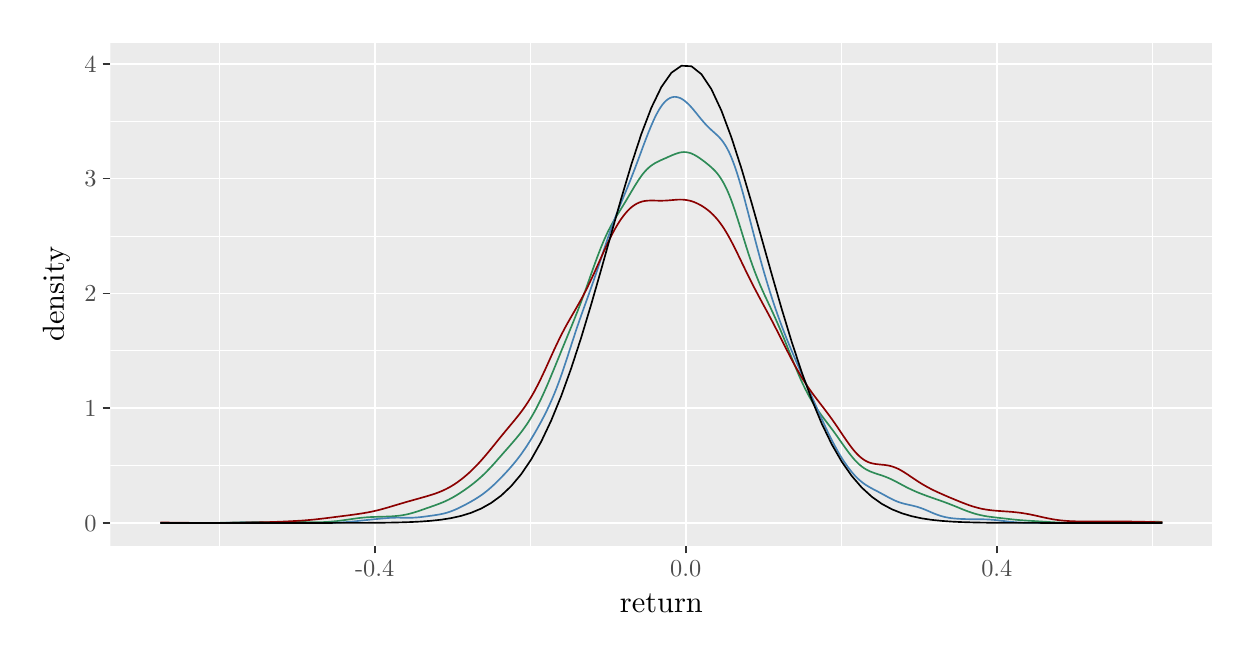
\begin{tikzpicture}[x=1pt,y=1pt]
\definecolor{fillColor}{RGB}{255,255,255}
\path[use as bounding box,fill=fillColor,fill opacity=0.00] (0,0) rectangle (433.62,216.81);
\begin{scope}
\path[clip] (  0.00,  0.00) rectangle (433.62,216.81);
\definecolor{drawColor}{RGB}{255,255,255}
\definecolor{fillColor}{RGB}{255,255,255}

\path[draw=drawColor,line width= 0.6pt,line join=round,line cap=round,fill=fillColor] (  0.00,  0.00) rectangle (433.62,216.81);
\end{scope}
\begin{scope}
\path[clip] ( 29.87, 29.59) rectangle (428.12,211.31);
\definecolor{fillColor}{gray}{0.92}

\path[fill=fillColor] ( 29.87, 29.59) rectangle (428.12,211.31);
\definecolor{drawColor}{RGB}{255,255,255}

\path[draw=drawColor,line width= 0.3pt,line join=round] ( 29.87, 58.58) --
	(428.12, 58.58);

\path[draw=drawColor,line width= 0.3pt,line join=round] ( 29.87,100.06) --
	(428.12,100.06);

\path[draw=drawColor,line width= 0.3pt,line join=round] ( 29.87,141.53) --
	(428.12,141.53);

\path[draw=drawColor,line width= 0.3pt,line join=round] ( 29.87,183.01) --
	(428.12,183.01);

\path[draw=drawColor,line width= 0.3pt,line join=round] ( 69.21, 29.59) --
	( 69.21,211.31);

\path[draw=drawColor,line width= 0.3pt,line join=round] (181.61, 29.59) --
	(181.61,211.31);

\path[draw=drawColor,line width= 0.3pt,line join=round] (294.01, 29.59) --
	(294.01,211.31);

\path[draw=drawColor,line width= 0.3pt,line join=round] (406.41, 29.59) --
	(406.41,211.31);

\path[draw=drawColor,line width= 0.6pt,line join=round] ( 29.87, 37.85) --
	(428.12, 37.85);

\path[draw=drawColor,line width= 0.6pt,line join=round] ( 29.87, 79.32) --
	(428.12, 79.32);

\path[draw=drawColor,line width= 0.6pt,line join=round] ( 29.87,120.80) --
	(428.12,120.80);

\path[draw=drawColor,line width= 0.6pt,line join=round] ( 29.87,162.27) --
	(428.12,162.27);

\path[draw=drawColor,line width= 0.6pt,line join=round] ( 29.87,203.75) --
	(428.12,203.75);

\path[draw=drawColor,line width= 0.6pt,line join=round] (125.41, 29.59) --
	(125.41,211.31);

\path[draw=drawColor,line width= 0.6pt,line join=round] (237.81, 29.59) --
	(237.81,211.31);

\path[draw=drawColor,line width= 0.6pt,line join=round] (350.21, 29.59) --
	(350.21,211.31);
\definecolor{drawColor}{RGB}{46,139,87}

\path[draw=drawColor,line width= 0.6pt,line join=round] ( 47.97, 37.85) --
	( 48.68, 37.85) --
	( 49.39, 37.85) --
	( 50.10, 37.85) --
	( 50.81, 37.85) --
	( 51.51, 37.85) --
	( 52.22, 37.85) --
	( 52.93, 37.85) --
	( 53.64, 37.85) --
	( 54.35, 37.85) --
	( 55.06, 37.85) --
	( 55.76, 37.85) --
	( 56.47, 37.85) --
	( 57.18, 37.85) --
	( 57.89, 37.85) --
	( 58.60, 37.85) --
	( 59.31, 37.85) --
	( 60.02, 37.85) --
	( 60.72, 37.85) --
	( 61.43, 37.85) --
	( 62.14, 37.85) --
	( 62.85, 37.85) --
	( 63.56, 37.85) --
	( 64.27, 37.85) --
	( 64.98, 37.85) --
	( 65.68, 37.85) --
	( 66.39, 37.86) --
	( 67.10, 37.86) --
	( 67.81, 37.86) --
	( 68.52, 37.87) --
	( 69.23, 37.88) --
	( 69.93, 37.89) --
	( 70.64, 37.90) --
	( 71.35, 37.91) --
	( 72.06, 37.92) --
	( 72.77, 37.94) --
	( 73.48, 37.96) --
	( 74.19, 37.98) --
	( 74.89, 38.00) --
	( 75.60, 38.02) --
	( 76.31, 38.05) --
	( 77.02, 38.07) --
	( 77.73, 38.09) --
	( 78.44, 38.11) --
	( 79.15, 38.13) --
	( 79.85, 38.14) --
	( 80.56, 38.15) --
	( 81.27, 38.16) --
	( 81.98, 38.17) --
	( 82.69, 38.17) --
	( 83.40, 38.17) --
	( 84.10, 38.16) --
	( 84.81, 38.16) --
	( 85.52, 38.15) --
	( 86.23, 38.14) --
	( 86.94, 38.13) --
	( 87.65, 38.12) --
	( 88.36, 38.12) --
	( 89.06, 38.12) --
	( 89.77, 38.12) --
	( 90.48, 38.12) --
	( 91.19, 38.13) --
	( 91.90, 38.14) --
	( 92.61, 38.15) --
	( 93.32, 38.16) --
	( 94.02, 38.17) --
	( 94.73, 38.18) --
	( 95.44, 38.19) --
	( 96.15, 38.19) --
	( 96.86, 38.19) --
	( 97.57, 38.19) --
	( 98.28, 38.19) --
	( 98.98, 38.18) --
	( 99.69, 38.17) --
	(100.40, 38.16) --
	(101.11, 38.14) --
	(101.82, 38.13) --
	(102.53, 38.12) --
	(103.23, 38.11) --
	(103.94, 38.11) --
	(104.65, 38.11) --
	(105.36, 38.12) --
	(106.07, 38.13) --
	(106.78, 38.15) --
	(107.49, 38.18) --
	(108.19, 38.22) --
	(108.90, 38.26) --
	(109.61, 38.32) --
	(110.32, 38.38) --
	(111.03, 38.45) --
	(111.74, 38.52) --
	(112.45, 38.61) --
	(113.15, 38.70) --
	(113.86, 38.79) --
	(114.57, 38.89) --
	(115.28, 38.99) --
	(115.99, 39.10) --
	(116.70, 39.20) --
	(117.40, 39.30) --
	(118.11, 39.40) --
	(118.82, 39.50) --
	(119.53, 39.59) --
	(120.24, 39.67) --
	(120.95, 39.74) --
	(121.66, 39.81) --
	(122.36, 39.87) --
	(123.07, 39.92) --
	(123.78, 39.96) --
	(124.49, 39.99) --
	(125.20, 40.02) --
	(125.91, 40.04) --
	(126.62, 40.06) --
	(127.32, 40.08) --
	(128.03, 40.10) --
	(128.74, 40.12) --
	(129.45, 40.14) --
	(130.16, 40.16) --
	(130.87, 40.20) --
	(131.57, 40.23) --
	(132.28, 40.28) --
	(132.99, 40.34) --
	(133.70, 40.41) --
	(134.41, 40.49) --
	(135.12, 40.59) --
	(135.83, 40.71) --
	(136.53, 40.84) --
	(137.24, 40.99) --
	(137.95, 41.16) --
	(138.66, 41.35) --
	(139.37, 41.55) --
	(140.08, 41.77) --
	(140.79, 41.99) --
	(141.49, 42.23) --
	(142.20, 42.47) --
	(142.91, 42.72) --
	(143.62, 42.97) --
	(144.33, 43.22) --
	(145.04, 43.46) --
	(145.74, 43.71) --
	(146.45, 43.96) --
	(147.16, 44.21) --
	(147.87, 44.47) --
	(148.58, 44.73) --
	(149.29, 45.01) --
	(150.00, 45.30) --
	(150.70, 45.60) --
	(151.41, 45.93) --
	(152.12, 46.27) --
	(152.83, 46.64) --
	(153.54, 47.02) --
	(154.25, 47.43) --
	(154.96, 47.85) --
	(155.66, 48.29) --
	(156.37, 48.74) --
	(157.08, 49.21) --
	(157.79, 49.70) --
	(158.50, 50.20) --
	(159.21, 50.71) --
	(159.92, 51.23) --
	(160.62, 51.77) --
	(161.33, 52.33) --
	(162.04, 52.91) --
	(162.75, 53.51) --
	(163.46, 54.13) --
	(164.17, 54.77) --
	(164.87, 55.44) --
	(165.58, 56.14) --
	(166.29, 56.87) --
	(167.00, 57.61) --
	(167.71, 58.37) --
	(168.42, 59.15) --
	(169.13, 59.94) --
	(169.83, 60.75) --
	(170.54, 61.55) --
	(171.25, 62.36) --
	(171.96, 63.17) --
	(172.67, 63.97) --
	(173.38, 64.78) --
	(174.09, 65.58) --
	(174.79, 66.39) --
	(175.50, 67.21) --
	(176.21, 68.04) --
	(176.92, 68.89) --
	(177.63, 69.76) --
	(178.34, 70.66) --
	(179.04, 71.61) --
	(179.75, 72.59) --
	(180.46, 73.63) --
	(181.17, 74.71) --
	(181.88, 75.86) --
	(182.59, 77.06) --
	(183.30, 78.32) --
	(184.00, 79.65) --
	(184.71, 81.05) --
	(185.42, 82.50) --
	(186.13, 84.02) --
	(186.84, 85.58) --
	(187.55, 87.19) --
	(188.26, 88.84) --
	(188.96, 90.53) --
	(189.67, 92.24) --
	(190.38, 93.96) --
	(191.09, 95.70) --
	(191.80, 97.44) --
	(192.51, 99.17) --
	(193.21,100.90) --
	(193.92,102.63) --
	(194.63,104.35) --
	(195.34,106.07) --
	(196.05,107.79) --
	(196.76,109.52) --
	(197.47,111.27) --
	(198.17,113.04) --
	(198.88,114.84) --
	(199.59,116.69) --
	(200.30,118.56) --
	(201.01,120.48) --
	(201.72,122.43) --
	(202.43,124.41) --
	(203.13,126.42) --
	(203.84,128.42) --
	(204.55,130.42) --
	(205.26,132.38) --
	(205.97,134.30) --
	(206.68,136.15) --
	(207.39,137.94) --
	(208.09,139.63) --
	(208.80,141.24) --
	(209.51,142.75) --
	(210.22,144.16) --
	(210.93,145.49) --
	(211.64,146.75) --
	(212.34,147.96) --
	(213.05,149.13) --
	(213.76,150.28) --
	(214.47,151.43) --
	(215.18,152.58) --
	(215.89,153.75) --
	(216.60,154.93) --
	(217.30,156.13) --
	(218.01,157.33) --
	(218.72,158.53) --
	(219.43,159.70) --
	(220.14,160.84) --
	(220.85,161.93) --
	(221.56,162.96) --
	(222.26,163.91) --
	(222.97,164.76) --
	(223.68,165.52) --
	(224.39,166.20) --
	(225.10,166.79) --
	(225.81,167.30) --
	(226.51,167.75) --
	(227.22,168.15) --
	(227.93,168.50) --
	(228.64,168.84) --
	(229.35,169.16) --
	(230.06,169.47) --
	(230.77,169.78) --
	(231.47,170.10) --
	(232.18,170.41) --
	(232.89,170.72) --
	(233.60,171.01) --
	(234.31,171.28) --
	(235.02,171.51) --
	(235.73,171.70) --
	(236.43,171.81) --
	(237.14,171.86) --
	(237.85,171.83) --
	(238.56,171.72) --
	(239.27,171.54) --
	(239.98,171.29) --
	(240.68,170.96) --
	(241.39,170.58) --
	(242.10,170.14) --
	(242.81,169.67) --
	(243.52,169.16) --
	(244.23,168.64) --
	(244.94,168.09) --
	(245.64,167.53) --
	(246.35,166.94) --
	(247.06,166.32) --
	(247.77,165.65) --
	(248.48,164.93) --
	(249.19,164.11) --
	(249.90,163.19) --
	(250.60,162.14) --
	(251.31,160.96) --
	(252.02,159.63) --
	(252.73,158.15) --
	(253.44,156.51) --
	(254.15,154.72) --
	(254.85,152.78) --
	(255.56,150.71) --
	(256.27,148.54) --
	(256.98,146.30) --
	(257.69,144.02) --
	(258.40,141.71) --
	(259.11,139.42) --
	(259.81,137.17) --
	(260.52,134.97) --
	(261.23,132.84) --
	(261.94,130.81) --
	(262.65,128.88) --
	(263.36,127.03) --
	(264.07,125.27) --
	(264.77,123.59) --
	(265.48,121.97) --
	(266.19,120.40) --
	(266.90,118.87) --
	(267.61,117.35) --
	(268.32,115.84) --
	(269.03,114.31) --
	(269.73,112.76) --
	(270.44,111.18) --
	(271.15,109.56) --
	(271.86,107.91) --
	(272.57,106.22) --
	(273.28,104.49) --
	(273.98,102.74) --
	(274.69,100.97) --
	(275.40, 99.20) --
	(276.11, 97.43) --
	(276.82, 95.67) --
	(277.53, 93.95) --
	(278.24, 92.26) --
	(278.94, 90.62) --
	(279.65, 89.04) --
	(280.36, 87.52) --
	(281.07, 86.07) --
	(281.78, 84.70) --
	(282.49, 83.40) --
	(283.20, 82.17) --
	(283.90, 81.01) --
	(284.61, 79.91) --
	(285.32, 78.85) --
	(286.03, 77.85) --
	(286.74, 76.87) --
	(287.45, 75.93) --
	(288.15, 74.99) --
	(288.86, 74.06) --
	(289.57, 73.13) --
	(290.28, 72.19) --
	(290.99, 71.23) --
	(291.70, 70.26) --
	(292.41, 69.27) --
	(293.11, 68.27) --
	(293.82, 67.26) --
	(294.53, 66.25) --
	(295.24, 65.25) --
	(295.95, 64.27) --
	(296.66, 63.31) --
	(297.37, 62.39) --
	(298.07, 61.52) --
	(298.78, 60.69) --
	(299.49, 59.93) --
	(300.20, 59.24) --
	(300.91, 58.62) --
	(301.62, 58.07) --
	(302.32, 57.58) --
	(303.03, 57.15) --
	(303.74, 56.78) --
	(304.45, 56.45) --
	(305.16, 56.17) --
	(305.87, 55.91) --
	(306.58, 55.67) --
	(307.28, 55.44) --
	(307.99, 55.21) --
	(308.70, 54.98) --
	(309.41, 54.73) --
	(310.12, 54.46) --
	(310.83, 54.17) --
	(311.54, 53.86) --
	(312.24, 53.53) --
	(312.95, 53.18) --
	(313.66, 52.82) --
	(314.37, 52.45) --
	(315.08, 52.07) --
	(315.79, 51.69) --
	(316.49, 51.31) --
	(317.20, 50.94) --
	(317.91, 50.58) --
	(318.62, 50.23) --
	(319.33, 49.89) --
	(320.04, 49.57) --
	(320.75, 49.25) --
	(321.45, 48.95) --
	(322.16, 48.66) --
	(322.87, 48.38) --
	(323.58, 48.11) --
	(324.29, 47.84) --
	(325.00, 47.58) --
	(325.71, 47.33) --
	(326.41, 47.08) --
	(327.12, 46.83) --
	(327.83, 46.58) --
	(328.54, 46.34) --
	(329.25, 46.09) --
	(329.96, 45.84) --
	(330.67, 45.59) --
	(331.37, 45.33) --
	(332.08, 45.07) --
	(332.79, 44.80) --
	(333.50, 44.52) --
	(334.21, 44.24) --
	(334.92, 43.96) --
	(335.62, 43.67) --
	(336.33, 43.38) --
	(337.04, 43.09) --
	(337.75, 42.80) --
	(338.46, 42.52) --
	(339.17, 42.24) --
	(339.88, 41.98) --
	(340.58, 41.73) --
	(341.29, 41.49) --
	(342.00, 41.27) --
	(342.71, 41.06) --
	(343.42, 40.88) --
	(344.13, 40.71) --
	(344.84, 40.55) --
	(345.54, 40.42) --
	(346.25, 40.29) --
	(346.96, 40.18) --
	(347.67, 40.08) --
	(348.38, 39.99) --
	(349.09, 39.90) --
	(349.79, 39.82) --
	(350.50, 39.73) --
	(351.21, 39.65) --
	(351.92, 39.57) --
	(352.63, 39.49) --
	(353.34, 39.41) --
	(354.05, 39.33) --
	(354.75, 39.25) --
	(355.46, 39.17) --
	(356.17, 39.09) --
	(356.88, 39.02) --
	(357.59, 38.95) --
	(358.30, 38.89) --
	(359.01, 38.83) --
	(359.71, 38.78) --
	(360.42, 38.73) --
	(361.13, 38.68) --
	(361.84, 38.64) --
	(362.55, 38.59) --
	(363.26, 38.55) --
	(363.96, 38.51) --
	(364.67, 38.47) --
	(365.38, 38.42) --
	(366.09, 38.38) --
	(366.80, 38.33) --
	(367.51, 38.29) --
	(368.22, 38.24) --
	(368.92, 38.19) --
	(369.63, 38.15) --
	(370.34, 38.11) --
	(371.05, 38.07) --
	(371.76, 38.03) --
	(372.47, 38.00) --
	(373.18, 37.97) --
	(373.88, 37.95) --
	(374.59, 37.92) --
	(375.30, 37.91) --
	(376.01, 37.89) --
	(376.72, 37.88) --
	(377.43, 37.87) --
	(378.13, 37.87) --
	(378.84, 37.86) --
	(379.55, 37.86) --
	(380.26, 37.85) --
	(380.97, 37.85) --
	(381.68, 37.85) --
	(382.39, 37.85) --
	(383.09, 37.85) --
	(383.80, 37.85) --
	(384.51, 37.85) --
	(385.22, 37.85) --
	(385.93, 37.85) --
	(386.64, 37.85) --
	(387.35, 37.85) --
	(388.05, 37.86) --
	(388.76, 37.86) --
	(389.47, 37.86) --
	(390.18, 37.87) --
	(390.89, 37.88) --
	(391.60, 37.88) --
	(392.31, 37.89) --
	(393.01, 37.91) --
	(393.72, 37.92) --
	(394.43, 37.93) --
	(395.14, 37.95) --
	(395.85, 37.97) --
	(396.56, 37.99) --
	(397.26, 38.01) --
	(397.97, 38.03) --
	(398.68, 38.05) --
	(399.39, 38.08) --
	(400.10, 38.10) --
	(400.81, 38.12) --
	(401.52, 38.15) --
	(402.22, 38.17) --
	(402.93, 38.19) --
	(403.64, 38.21) --
	(404.35, 38.22) --
	(405.06, 38.24) --
	(405.77, 38.25) --
	(406.48, 38.25) --
	(407.18, 38.26) --
	(407.89, 38.25) --
	(408.60, 38.25) --
	(409.31, 38.24) --
	(410.02, 38.22);
\definecolor{drawColor}{RGB}{70,130,180}

\path[draw=drawColor,line width= 0.6pt,line join=round] ( 47.97, 37.85) --
	( 48.68, 37.85) --
	( 49.39, 37.85) --
	( 50.10, 37.85) --
	( 50.81, 37.85) --
	( 51.51, 37.85) --
	( 52.22, 37.85) --
	( 52.93, 37.85) --
	( 53.64, 37.85) --
	( 54.35, 37.85) --
	( 55.06, 37.85) --
	( 55.76, 37.85) --
	( 56.47, 37.85) --
	( 57.18, 37.85) --
	( 57.89, 37.85) --
	( 58.60, 37.85) --
	( 59.31, 37.85) --
	( 60.02, 37.85) --
	( 60.72, 37.85) --
	( 61.43, 37.85) --
	( 62.14, 37.85) --
	( 62.85, 37.85) --
	( 63.56, 37.85) --
	( 64.27, 37.85) --
	( 64.98, 37.85) --
	( 65.68, 37.85) --
	( 66.39, 37.85) --
	( 67.10, 37.85) --
	( 67.81, 37.85) --
	( 68.52, 37.86) --
	( 69.23, 37.86) --
	( 69.93, 37.86) --
	( 70.64, 37.87) --
	( 71.35, 37.88) --
	( 72.06, 37.89) --
	( 72.77, 37.90) --
	( 73.48, 37.91) --
	( 74.19, 37.93) --
	( 74.89, 37.94) --
	( 75.60, 37.96) --
	( 76.31, 37.97) --
	( 77.02, 37.99) --
	( 77.73, 38.00) --
	( 78.44, 38.02) --
	( 79.15, 38.02) --
	( 79.85, 38.03) --
	( 80.56, 38.03) --
	( 81.27, 38.03) --
	( 81.98, 38.03) --
	( 82.69, 38.02) --
	( 83.40, 38.01) --
	( 84.10, 38.00) --
	( 84.81, 37.98) --
	( 85.52, 37.96) --
	( 86.23, 37.95) --
	( 86.94, 37.93) --
	( 87.65, 37.92) --
	( 88.36, 37.90) --
	( 89.06, 37.89) --
	( 89.77, 37.88) --
	( 90.48, 37.87) --
	( 91.19, 37.87) --
	( 91.90, 37.86) --
	( 92.61, 37.86) --
	( 93.32, 37.85) --
	( 94.02, 37.85) --
	( 94.73, 37.85) --
	( 95.44, 37.85) --
	( 96.15, 37.85) --
	( 96.86, 37.85) --
	( 97.57, 37.85) --
	( 98.28, 37.85) --
	( 98.98, 37.85) --
	( 99.69, 37.85) --
	(100.40, 37.85) --
	(101.11, 37.85) --
	(101.82, 37.85) --
	(102.53, 37.85) --
	(103.23, 37.85) --
	(103.94, 37.85) --
	(104.65, 37.85) --
	(105.36, 37.85) --
	(106.07, 37.85) --
	(106.78, 37.86) --
	(107.49, 37.86) --
	(108.19, 37.87) --
	(108.90, 37.88) --
	(109.61, 37.89) --
	(110.32, 37.91) --
	(111.03, 37.93) --
	(111.74, 37.96) --
	(112.45, 37.99) --
	(113.15, 38.02) --
	(113.86, 38.06) --
	(114.57, 38.11) --
	(115.28, 38.17) --
	(115.99, 38.23) --
	(116.70, 38.29) --
	(117.40, 38.36) --
	(118.11, 38.43) --
	(118.82, 38.50) --
	(119.53, 38.58) --
	(120.24, 38.66) --
	(120.95, 38.73) --
	(121.66, 38.81) --
	(122.36, 38.88) --
	(123.07, 38.95) --
	(123.78, 39.03) --
	(124.49, 39.10) --
	(125.20, 39.17) --
	(125.91, 39.24) --
	(126.62, 39.31) --
	(127.32, 39.38) --
	(128.03, 39.44) --
	(128.74, 39.51) --
	(129.45, 39.57) --
	(130.16, 39.62) --
	(130.87, 39.67) --
	(131.57, 39.70) --
	(132.28, 39.73) --
	(132.99, 39.75) --
	(133.70, 39.75) --
	(134.41, 39.75) --
	(135.12, 39.74) --
	(135.83, 39.73) --
	(136.53, 39.72) --
	(137.24, 39.71) --
	(137.95, 39.71) --
	(138.66, 39.73) --
	(139.37, 39.75) --
	(140.08, 39.79) --
	(140.79, 39.84) --
	(141.49, 39.91) --
	(142.20, 39.98) --
	(142.91, 40.07) --
	(143.62, 40.16) --
	(144.33, 40.25) --
	(145.04, 40.35) --
	(145.74, 40.45) --
	(146.45, 40.54) --
	(147.16, 40.65) --
	(147.87, 40.76) --
	(148.58, 40.88) --
	(149.29, 41.01) --
	(150.00, 41.16) --
	(150.70, 41.33) --
	(151.41, 41.53) --
	(152.12, 41.74) --
	(152.83, 41.99) --
	(153.54, 42.26) --
	(154.25, 42.55) --
	(154.96, 42.86) --
	(155.66, 43.19) --
	(156.37, 43.53) --
	(157.08, 43.89) --
	(157.79, 44.25) --
	(158.50, 44.63) --
	(159.21, 45.01) --
	(159.92, 45.40) --
	(160.62, 45.81) --
	(161.33, 46.22) --
	(162.04, 46.65) --
	(162.75, 47.10) --
	(163.46, 47.57) --
	(164.17, 48.06) --
	(164.87, 48.58) --
	(165.58, 49.13) --
	(166.29, 49.70) --
	(167.00, 50.31) --
	(167.71, 50.94) --
	(168.42, 51.59) --
	(169.13, 52.27) --
	(169.83, 52.96) --
	(170.54, 53.67) --
	(171.25, 54.40) --
	(171.96, 55.14) --
	(172.67, 55.89) --
	(173.38, 56.66) --
	(174.09, 57.45) --
	(174.79, 58.26) --
	(175.50, 59.09) --
	(176.21, 59.95) --
	(176.92, 60.84) --
	(177.63, 61.76) --
	(178.34, 62.72) --
	(179.04, 63.72) --
	(179.75, 64.75) --
	(180.46, 65.82) --
	(181.17, 66.93) --
	(181.88, 68.07) --
	(182.59, 69.24) --
	(183.30, 70.44) --
	(184.00, 71.67) --
	(184.71, 72.94) --
	(185.42, 74.23) --
	(186.13, 75.57) --
	(186.84, 76.95) --
	(187.55, 78.38) --
	(188.26, 79.87) --
	(188.96, 81.42) --
	(189.67, 83.03) --
	(190.38, 84.73) --
	(191.09, 86.51) --
	(191.80, 88.37) --
	(192.51, 90.32) --
	(193.21, 92.34) --
	(193.92, 94.44) --
	(194.63, 96.59) --
	(195.34, 98.77) --
	(196.05,100.96) --
	(196.76,103.15) --
	(197.47,105.33) --
	(198.17,107.47) --
	(198.88,109.57) --
	(199.59,111.62) --
	(200.30,113.64) --
	(201.01,115.62) --
	(201.72,117.58) --
	(202.43,119.55) --
	(203.13,121.52) --
	(203.84,123.52) --
	(204.55,125.55) --
	(205.26,127.62) --
	(205.97,129.72) --
	(206.68,131.86) --
	(207.39,134.01) --
	(208.09,136.16) --
	(208.80,138.30) --
	(209.51,140.41) --
	(210.22,142.47) --
	(210.93,144.47) --
	(211.64,146.42) --
	(212.34,148.30) --
	(213.05,150.12) --
	(213.76,151.89) --
	(214.47,153.62) --
	(215.18,155.34) --
	(215.89,157.05) --
	(216.60,158.77) --
	(217.30,160.52) --
	(218.01,162.29) --
	(218.72,164.11) --
	(219.43,165.95) --
	(220.14,167.83) --
	(220.85,169.74) --
	(221.56,171.65) --
	(222.26,173.57) --
	(222.97,175.46) --
	(223.68,177.32) --
	(224.39,179.13) --
	(225.10,180.86) --
	(225.81,182.51) --
	(226.51,184.06) --
	(227.22,185.49) --
	(227.93,186.79) --
	(228.64,187.96) --
	(229.35,188.96) --
	(230.06,189.81) --
	(230.77,190.50) --
	(231.47,191.04) --
	(232.18,191.43) --
	(232.89,191.68) --
	(233.60,191.80) --
	(234.31,191.78) --
	(235.02,191.64) --
	(235.73,191.39) --
	(236.43,191.03) --
	(237.14,190.56) --
	(237.85,190.00) --
	(238.56,189.35) --
	(239.27,188.64) --
	(239.98,187.86) --
	(240.68,187.04) --
	(241.39,186.18) --
	(242.10,185.30) --
	(242.81,184.42) --
	(243.52,183.55) --
	(244.23,182.72) --
	(244.94,181.93) --
	(245.64,181.19) --
	(246.35,180.49) --
	(247.06,179.83) --
	(247.77,179.19) --
	(248.48,178.55) --
	(249.19,177.90) --
	(249.90,177.19) --
	(250.60,176.40) --
	(251.31,175.49) --
	(252.02,174.43) --
	(252.73,173.21) --
	(253.44,171.82) --
	(254.15,170.24) --
	(254.85,168.48) --
	(255.56,166.54) --
	(256.27,164.42) --
	(256.98,162.16) --
	(257.69,159.75) --
	(258.40,157.22) --
	(259.11,154.60) --
	(259.81,151.92) --
	(260.52,149.20) --
	(261.23,146.46) --
	(261.94,143.72) --
	(262.65,140.99) --
	(263.36,138.30) --
	(264.07,135.65) --
	(264.77,133.05) --
	(265.48,130.51) --
	(266.19,128.04) --
	(266.90,125.64) --
	(267.61,123.30) --
	(268.32,121.04) --
	(269.03,118.84) --
	(269.73,116.70) --
	(270.44,114.63) --
	(271.15,112.61) --
	(271.86,110.66) --
	(272.57,108.76) --
	(273.28,106.91) --
	(273.98,105.11) --
	(274.69,103.35) --
	(275.40,101.63) --
	(276.11, 99.94) --
	(276.82, 98.27) --
	(277.53, 96.63) --
	(278.24, 95.00) --
	(278.94, 93.39) --
	(279.65, 91.80) --
	(280.36, 90.20) --
	(281.07, 88.61) --
	(281.78, 87.02) --
	(282.49, 85.43) --
	(283.20, 83.83) --
	(283.90, 82.24) --
	(284.61, 80.64) --
	(285.32, 79.04) --
	(286.03, 77.44) --
	(286.74, 75.86) --
	(287.45, 74.30) --
	(288.15, 72.76) --
	(288.86, 71.25) --
	(289.57, 69.78) --
	(290.28, 68.35) --
	(290.99, 66.96) --
	(291.70, 65.62) --
	(292.41, 64.32) --
	(293.11, 63.08) --
	(293.82, 61.89) --
	(294.53, 60.76) --
	(295.24, 59.68) --
	(295.95, 58.65) --
	(296.66, 57.68) --
	(297.37, 56.76) --
	(298.07, 55.90) --
	(298.78, 55.10) --
	(299.49, 54.35) --
	(300.20, 53.67) --
	(300.91, 53.04) --
	(301.62, 52.47) --
	(302.32, 51.95) --
	(303.03, 51.47) --
	(303.74, 51.04) --
	(304.45, 50.63) --
	(305.16, 50.24) --
	(305.87, 49.86) --
	(306.58, 49.49) --
	(307.28, 49.13) --
	(307.99, 48.75) --
	(308.70, 48.37) --
	(309.41, 47.99) --
	(310.12, 47.60) --
	(310.83, 47.21) --
	(311.54, 46.84) --
	(312.24, 46.47) --
	(312.95, 46.13) --
	(313.66, 45.81) --
	(314.37, 45.52) --
	(315.08, 45.27) --
	(315.79, 45.04) --
	(316.49, 44.85) --
	(317.20, 44.67) --
	(317.91, 44.51) --
	(318.62, 44.35) --
	(319.33, 44.20) --
	(320.04, 44.03) --
	(320.75, 43.85) --
	(321.45, 43.66) --
	(322.16, 43.43) --
	(322.87, 43.19) --
	(323.58, 42.92) --
	(324.29, 42.63) --
	(325.00, 42.34) --
	(325.71, 42.03) --
	(326.41, 41.72) --
	(327.12, 41.42) --
	(327.83, 41.13) --
	(328.54, 40.86) --
	(329.25, 40.61) --
	(329.96, 40.38) --
	(330.67, 40.18) --
	(331.37, 40.00) --
	(332.08, 39.85) --
	(332.79, 39.72) --
	(333.50, 39.61) --
	(334.21, 39.52) --
	(334.92, 39.45) --
	(335.62, 39.39) --
	(336.33, 39.34) --
	(337.04, 39.30) --
	(337.75, 39.27) --
	(338.46, 39.25) --
	(339.17, 39.23) --
	(339.88, 39.21) --
	(340.58, 39.20) --
	(341.29, 39.19) --
	(342.00, 39.19) --
	(342.71, 39.19) --
	(343.42, 39.18) --
	(344.13, 39.18) --
	(344.84, 39.17) --
	(345.54, 39.15) --
	(346.25, 39.13) --
	(346.96, 39.10) --
	(347.67, 39.06) --
	(348.38, 39.01) --
	(349.09, 38.95) --
	(349.79, 38.88) --
	(350.50, 38.81) --
	(351.21, 38.73) --
	(351.92, 38.64) --
	(352.63, 38.56) --
	(353.34, 38.47) --
	(354.05, 38.39) --
	(354.75, 38.31) --
	(355.46, 38.23) --
	(356.17, 38.17) --
	(356.88, 38.11) --
	(357.59, 38.05) --
	(358.30, 38.01) --
	(359.01, 37.97) --
	(359.71, 37.94) --
	(360.42, 37.92) --
	(361.13, 37.90) --
	(361.84, 37.89) --
	(362.55, 37.87) --
	(363.26, 37.87) --
	(363.96, 37.86) --
	(364.67, 37.86) --
	(365.38, 37.85) --
	(366.09, 37.85) --
	(366.80, 37.85) --
	(367.51, 37.85) --
	(368.22, 37.85) --
	(368.92, 37.85) --
	(369.63, 37.85) --
	(370.34, 37.85) --
	(371.05, 37.85) --
	(371.76, 37.85) --
	(372.47, 37.85) --
	(373.18, 37.85) --
	(373.88, 37.85) --
	(374.59, 37.85) --
	(375.30, 37.85) --
	(376.01, 37.85) --
	(376.72, 37.86) --
	(377.43, 37.86) --
	(378.13, 37.86) --
	(378.84, 37.87) --
	(379.55, 37.88) --
	(380.26, 37.88) --
	(380.97, 37.90) --
	(381.68, 37.91) --
	(382.39, 37.92) --
	(383.09, 37.94) --
	(383.80, 37.95) --
	(384.51, 37.97) --
	(385.22, 37.98) --
	(385.93, 38.00) --
	(386.64, 38.01) --
	(387.35, 38.02) --
	(388.05, 38.03) --
	(388.76, 38.03) --
	(389.47, 38.03) --
	(390.18, 38.03) --
	(390.89, 38.02) --
	(391.60, 38.01) --
	(392.31, 38.00) --
	(393.01, 37.99) --
	(393.72, 37.97) --
	(394.43, 37.95) --
	(395.14, 37.94) --
	(395.85, 37.92) --
	(396.56, 37.91) --
	(397.26, 37.90) --
	(397.97, 37.89) --
	(398.68, 37.88) --
	(399.39, 37.87) --
	(400.10, 37.86) --
	(400.81, 37.86) --
	(401.52, 37.86) --
	(402.22, 37.85) --
	(402.93, 37.85) --
	(403.64, 37.85) --
	(404.35, 37.85) --
	(405.06, 37.85) --
	(405.77, 37.85) --
	(406.48, 37.85) --
	(407.18, 37.85) --
	(407.89, 37.85) --
	(408.60, 37.85) --
	(409.31, 37.85) --
	(410.02, 37.85);
\definecolor{drawColor}{RGB}{139,0,0}

\path[draw=drawColor,line width= 0.6pt,line join=round] ( 47.97, 37.99) --
	( 48.68, 37.99) --
	( 49.39, 37.99) --
	( 50.10, 37.99) --
	( 50.81, 37.98) --
	( 51.51, 37.97) --
	( 52.22, 37.96) --
	( 52.93, 37.95) --
	( 53.64, 37.95) --
	( 54.35, 37.94) --
	( 55.06, 37.93) --
	( 55.76, 37.92) --
	( 56.47, 37.91) --
	( 57.18, 37.90) --
	( 57.89, 37.89) --
	( 58.60, 37.88) --
	( 59.31, 37.88) --
	( 60.02, 37.87) --
	( 60.72, 37.87) --
	( 61.43, 37.86) --
	( 62.14, 37.86) --
	( 62.85, 37.86) --
	( 63.56, 37.86) --
	( 64.27, 37.85) --
	( 64.98, 37.85) --
	( 65.68, 37.85) --
	( 66.39, 37.85) --
	( 67.10, 37.85) --
	( 67.81, 37.86) --
	( 68.52, 37.86) --
	( 69.23, 37.86) --
	( 69.93, 37.86) --
	( 70.64, 37.87) --
	( 71.35, 37.87) --
	( 72.06, 37.88) --
	( 72.77, 37.88) --
	( 73.48, 37.89) --
	( 74.19, 37.90) --
	( 74.89, 37.91) --
	( 75.60, 37.92) --
	( 76.31, 37.93) --
	( 77.02, 37.94) --
	( 77.73, 37.95) --
	( 78.44, 37.97) --
	( 79.15, 37.98) --
	( 79.85, 37.99) --
	( 80.56, 38.01) --
	( 81.27, 38.02) --
	( 81.98, 38.03) --
	( 82.69, 38.05) --
	( 83.40, 38.06) --
	( 84.10, 38.07) --
	( 84.81, 38.09) --
	( 85.52, 38.11) --
	( 86.23, 38.12) --
	( 86.94, 38.14) --
	( 87.65, 38.16) --
	( 88.36, 38.18) --
	( 89.06, 38.21) --
	( 89.77, 38.23) --
	( 90.48, 38.26) --
	( 91.19, 38.29) --
	( 91.90, 38.32) --
	( 92.61, 38.35) --
	( 93.32, 38.38) --
	( 94.02, 38.42) --
	( 94.73, 38.45) --
	( 95.44, 38.49) --
	( 96.15, 38.53) --
	( 96.86, 38.56) --
	( 97.57, 38.61) --
	( 98.28, 38.65) --
	( 98.98, 38.69) --
	( 99.69, 38.74) --
	(100.40, 38.80) --
	(101.11, 38.85) --
	(101.82, 38.92) --
	(102.53, 38.98) --
	(103.23, 39.05) --
	(103.94, 39.12) --
	(104.65, 39.20) --
	(105.36, 39.28) --
	(106.07, 39.36) --
	(106.78, 39.45) --
	(107.49, 39.53) --
	(108.19, 39.62) --
	(108.90, 39.71) --
	(109.61, 39.80) --
	(110.32, 39.89) --
	(111.03, 39.98) --
	(111.74, 40.07) --
	(112.45, 40.16) --
	(113.15, 40.25) --
	(113.86, 40.34) --
	(114.57, 40.43) --
	(115.28, 40.52) --
	(115.99, 40.61) --
	(116.70, 40.71) --
	(117.40, 40.80) --
	(118.11, 40.90) --
	(118.82, 41.00) --
	(119.53, 41.10) --
	(120.24, 41.21) --
	(120.95, 41.32) --
	(121.66, 41.44) --
	(122.36, 41.56) --
	(123.07, 41.69) --
	(123.78, 41.83) --
	(124.49, 41.97) --
	(125.20, 42.13) --
	(125.91, 42.29) --
	(126.62, 42.46) --
	(127.32, 42.64) --
	(128.03, 42.83) --
	(128.74, 43.03) --
	(129.45, 43.23) --
	(130.16, 43.43) --
	(130.87, 43.64) --
	(131.57, 43.85) --
	(132.28, 44.07) --
	(132.99, 44.28) --
	(133.70, 44.49) --
	(134.41, 44.70) --
	(135.12, 44.91) --
	(135.83, 45.12) --
	(136.53, 45.33) --
	(137.24, 45.53) --
	(137.95, 45.73) --
	(138.66, 45.93) --
	(139.37, 46.13) --
	(140.08, 46.33) --
	(140.79, 46.52) --
	(141.49, 46.72) --
	(142.20, 46.92) --
	(142.91, 47.12) --
	(143.62, 47.32) --
	(144.33, 47.53) --
	(145.04, 47.74) --
	(145.74, 47.96) --
	(146.45, 48.18) --
	(147.16, 48.42) --
	(147.87, 48.67) --
	(148.58, 48.94) --
	(149.29, 49.23) --
	(150.00, 49.53) --
	(150.70, 49.86) --
	(151.41, 50.21) --
	(152.12, 50.58) --
	(152.83, 50.98) --
	(153.54, 51.40) --
	(154.25, 51.85) --
	(154.96, 52.32) --
	(155.66, 52.83) --
	(156.37, 53.35) --
	(157.08, 53.90) --
	(157.79, 54.48) --
	(158.50, 55.08) --
	(159.21, 55.70) --
	(159.92, 56.35) --
	(160.62, 57.03) --
	(161.33, 57.73) --
	(162.04, 58.45) --
	(162.75, 59.19) --
	(163.46, 59.96) --
	(164.17, 60.75) --
	(164.87, 61.56) --
	(165.58, 62.39) --
	(166.29, 63.23) --
	(167.00, 64.09) --
	(167.71, 64.96) --
	(168.42, 65.83) --
	(169.13, 66.71) --
	(169.83, 67.59) --
	(170.54, 68.46) --
	(171.25, 69.33) --
	(171.96, 70.19) --
	(172.67, 71.05) --
	(173.38, 71.90) --
	(174.09, 72.75) --
	(174.79, 73.60) --
	(175.50, 74.45) --
	(176.21, 75.31) --
	(176.92, 76.19) --
	(177.63, 77.08) --
	(178.34, 78.01) --
	(179.04, 78.97) --
	(179.75, 79.97) --
	(180.46, 81.02) --
	(181.17, 82.12) --
	(181.88, 83.27) --
	(182.59, 84.48) --
	(183.30, 85.76) --
	(184.00, 87.10) --
	(184.71, 88.49) --
	(185.42, 89.93) --
	(186.13, 91.42) --
	(186.84, 92.94) --
	(187.55, 94.49) --
	(188.26, 96.05) --
	(188.96, 97.62) --
	(189.67, 99.18) --
	(190.38,100.72) --
	(191.09,102.23) --
	(191.80,103.71) --
	(192.51,105.15) --
	(193.21,106.54) --
	(193.92,107.90) --
	(194.63,109.21) --
	(195.34,110.48) --
	(196.05,111.72) --
	(196.76,112.95) --
	(197.47,114.17) --
	(198.17,115.39) --
	(198.88,116.63) --
	(199.59,117.89) --
	(200.30,119.18) --
	(201.01,120.52) --
	(201.72,121.90) --
	(202.43,123.32) --
	(203.13,124.78) --
	(203.84,126.29) --
	(204.55,127.82) --
	(205.26,129.39) --
	(205.97,130.97) --
	(206.68,132.56) --
	(207.39,134.15) --
	(208.09,135.72) --
	(208.80,137.26) --
	(209.51,138.77) --
	(210.22,140.24) --
	(210.93,141.65) --
	(211.64,143.01) --
	(212.34,144.29) --
	(213.05,145.50) --
	(213.76,146.64) --
	(214.47,147.70) --
	(215.18,148.68) --
	(215.89,149.58) --
	(216.60,150.40) --
	(217.30,151.14) --
	(218.01,151.79) --
	(218.72,152.35) --
	(219.43,152.83) --
	(220.14,153.24) --
	(220.85,153.57) --
	(221.56,153.84) --
	(222.26,154.04) --
	(222.97,154.18) --
	(223.68,154.27) --
	(224.39,154.32) --
	(225.10,154.34) --
	(225.81,154.34) --
	(226.51,154.33) --
	(227.22,154.31) --
	(227.93,154.29) --
	(228.64,154.28) --
	(229.35,154.29) --
	(230.06,154.31) --
	(230.77,154.34) --
	(231.47,154.39) --
	(232.18,154.45) --
	(232.89,154.51) --
	(233.60,154.57) --
	(234.31,154.63) --
	(235.02,154.67) --
	(235.73,154.69) --
	(236.43,154.68) --
	(237.14,154.63) --
	(237.85,154.55) --
	(238.56,154.44) --
	(239.27,154.28) --
	(239.98,154.08) --
	(240.68,153.84) --
	(241.39,153.55) --
	(242.10,153.22) --
	(242.81,152.86) --
	(243.52,152.46) --
	(244.23,152.02) --
	(244.94,151.53) --
	(245.64,151.01) --
	(246.35,150.44) --
	(247.06,149.80) --
	(247.77,149.11) --
	(248.48,148.36) --
	(249.19,147.55) --
	(249.90,146.66) --
	(250.60,145.70) --
	(251.31,144.68) --
	(252.02,143.57) --
	(252.73,142.39) --
	(253.44,141.14) --
	(254.15,139.83) --
	(254.85,138.47) --
	(255.56,137.07) --
	(256.27,135.63) --
	(256.98,134.17) --
	(257.69,132.70) --
	(258.40,131.22) --
	(259.11,129.75) --
	(259.81,128.29) --
	(260.52,126.85) --
	(261.23,125.43) --
	(261.94,124.03) --
	(262.65,122.66) --
	(263.36,121.31) --
	(264.07,119.97) --
	(264.77,118.66) --
	(265.48,117.34) --
	(266.19,116.03) --
	(266.90,114.72) --
	(267.61,113.40) --
	(268.32,112.07) --
	(269.03,110.73) --
	(269.73,109.37) --
	(270.44,107.99) --
	(271.15,106.60) --
	(271.86,105.19) --
	(272.57,103.79) --
	(273.28,102.38) --
	(273.98,100.97) --
	(274.69, 99.57) --
	(275.40, 98.19) --
	(276.11, 96.84) --
	(276.82, 95.51) --
	(277.53, 94.21) --
	(278.24, 92.95) --
	(278.94, 91.73) --
	(279.65, 90.54) --
	(280.36, 89.39) --
	(281.07, 88.29) --
	(281.78, 87.23) --
	(282.49, 86.20) --
	(283.20, 85.20) --
	(283.90, 84.23) --
	(284.61, 83.28) --
	(285.32, 82.35) --
	(286.03, 81.43) --
	(286.74, 80.51) --
	(287.45, 79.59) --
	(288.15, 78.66) --
	(288.86, 77.72) --
	(289.57, 76.77) --
	(290.28, 75.79) --
	(290.99, 74.80) --
	(291.70, 73.79) --
	(292.41, 72.75) --
	(293.11, 71.71) --
	(293.82, 70.65) --
	(294.53, 69.60) --
	(295.24, 68.55) --
	(295.95, 67.52) --
	(296.66, 66.52) --
	(297.37, 65.55) --
	(298.07, 64.63) --
	(298.78, 63.78) --
	(299.49, 62.99) --
	(300.20, 62.27) --
	(300.91, 61.62) --
	(301.62, 61.06) --
	(302.32, 60.57) --
	(303.03, 60.16) --
	(303.74, 59.83) --
	(304.45, 59.57) --
	(305.16, 59.37) --
	(305.87, 59.22) --
	(306.58, 59.11) --
	(307.28, 59.03) --
	(307.99, 58.96) --
	(308.70, 58.89) --
	(309.41, 58.83) --
	(310.12, 58.74) --
	(310.83, 58.62) --
	(311.54, 58.47) --
	(312.24, 58.28) --
	(312.95, 58.05) --
	(313.66, 57.78) --
	(314.37, 57.47) --
	(315.08, 57.11) --
	(315.79, 56.72) --
	(316.49, 56.30) --
	(317.20, 55.85) --
	(317.91, 55.39) --
	(318.62, 54.91) --
	(319.33, 54.43) --
	(320.04, 53.95) --
	(320.75, 53.47) --
	(321.45, 53.00) --
	(322.16, 52.55) --
	(322.87, 52.11) --
	(323.58, 51.68) --
	(324.29, 51.27) --
	(325.00, 50.87) --
	(325.71, 50.49) --
	(326.41, 50.12) --
	(327.12, 49.77) --
	(327.83, 49.42) --
	(328.54, 49.09) --
	(329.25, 48.76) --
	(329.96, 48.45) --
	(330.67, 48.13) --
	(331.37, 47.82) --
	(332.08, 47.52) --
	(332.79, 47.21) --
	(333.50, 46.91) --
	(334.21, 46.62) --
	(334.92, 46.32) --
	(335.62, 46.03) --
	(336.33, 45.74) --
	(337.04, 45.45) --
	(337.75, 45.17) --
	(338.46, 44.90) --
	(339.17, 44.63) --
	(339.88, 44.37) --
	(340.58, 44.13) --
	(341.29, 43.89) --
	(342.00, 43.67) --
	(342.71, 43.47) --
	(343.42, 43.28) --
	(344.13, 43.10) --
	(344.84, 42.95) --
	(345.54, 42.81) --
	(346.25, 42.69) --
	(346.96, 42.58) --
	(347.67, 42.49) --
	(348.38, 42.40) --
	(349.09, 42.33) --
	(349.79, 42.27) --
	(350.50, 42.21) --
	(351.21, 42.16) --
	(351.92, 42.11) --
	(352.63, 42.06) --
	(353.34, 42.01) --
	(354.05, 41.97) --
	(354.75, 41.91) --
	(355.46, 41.86) --
	(356.17, 41.79) --
	(356.88, 41.72) --
	(357.59, 41.64) --
	(358.30, 41.56) --
	(359.01, 41.46) --
	(359.71, 41.36) --
	(360.42, 41.24) --
	(361.13, 41.12) --
	(361.84, 40.99) --
	(362.55, 40.85) --
	(363.26, 40.70) --
	(363.96, 40.55) --
	(364.67, 40.39) --
	(365.38, 40.23) --
	(366.09, 40.07) --
	(366.80, 39.91) --
	(367.51, 39.75) --
	(368.22, 39.60) --
	(368.92, 39.46) --
	(369.63, 39.32) --
	(370.34, 39.19) --
	(371.05, 39.07) --
	(371.76, 38.97) --
	(372.47, 38.87) --
	(373.18, 38.78) --
	(373.88, 38.71) --
	(374.59, 38.64) --
	(375.30, 38.59) --
	(376.01, 38.54) --
	(376.72, 38.50) --
	(377.43, 38.47) --
	(378.13, 38.44) --
	(378.84, 38.42) --
	(379.55, 38.40) --
	(380.26, 38.39) --
	(380.97, 38.38) --
	(381.68, 38.38) --
	(382.39, 38.38) --
	(383.09, 38.38) --
	(383.80, 38.38) --
	(384.51, 38.39) --
	(385.22, 38.39) --
	(385.93, 38.40) --
	(386.64, 38.40) --
	(387.35, 38.41) --
	(388.05, 38.41) --
	(388.76, 38.42) --
	(389.47, 38.42) --
	(390.18, 38.42) --
	(390.89, 38.42) --
	(391.60, 38.42) --
	(392.31, 38.42) --
	(393.01, 38.41) --
	(393.72, 38.41) --
	(394.43, 38.40) --
	(395.14, 38.39) --
	(395.85, 38.38) --
	(396.56, 38.37) --
	(397.26, 38.36) --
	(397.97, 38.35) --
	(398.68, 38.34) --
	(399.39, 38.33) --
	(400.10, 38.32) --
	(400.81, 38.30) --
	(401.52, 38.29) --
	(402.22, 38.28) --
	(402.93, 38.26) --
	(403.64, 38.25) --
	(404.35, 38.23) --
	(405.06, 38.21) --
	(405.77, 38.20) --
	(406.48, 38.18) --
	(407.18, 38.16) --
	(407.89, 38.14) --
	(408.60, 38.13) --
	(409.31, 38.11) --
	(410.02, 38.09);
\definecolor{drawColor}{RGB}{0,0,0}

\path[draw=drawColor,line width= 0.6pt,line join=round] ( 47.97, 37.85) --
	( 51.59, 37.85) --
	( 55.21, 37.85) --
	( 58.83, 37.85) --
	( 62.45, 37.85) --
	( 66.07, 37.85) --
	( 69.69, 37.85) --
	( 73.31, 37.85) --
	( 76.93, 37.85) --
	( 80.56, 37.85) --
	( 84.18, 37.85) --
	( 87.80, 37.85) --
	( 91.42, 37.85) --
	( 95.04, 37.85) --
	( 98.66, 37.85) --
	(102.28, 37.85) --
	(105.90, 37.85) --
	(109.52, 37.85) --
	(113.14, 37.86) --
	(116.76, 37.86) --
	(120.38, 37.87) --
	(124.00, 37.89) --
	(127.62, 37.92) --
	(131.24, 37.97) --
	(134.86, 38.05) --
	(138.48, 38.17) --
	(142.10, 38.35) --
	(145.72, 38.62) --
	(149.34, 39.01) --
	(152.96, 39.58) --
	(156.59, 40.38) --
	(160.21, 41.50) --
	(163.83, 43.02) --
	(167.45, 45.05) --
	(171.07, 47.70) --
	(174.69, 51.12) --
	(178.31, 55.43) --
	(181.93, 60.76) --
	(185.55, 67.20) --
	(189.17, 74.84) --
	(192.79, 83.70) --
	(196.41, 93.75) --
	(200.03,104.87) --
	(203.65,116.89) --
	(207.27,129.53) --
	(210.89,142.43) --
	(214.51,155.19) --
	(218.13,167.34) --
	(221.75,178.39) --
	(225.37,187.88) --
	(228.99,195.37) --
	(232.61,200.51) --
	(236.24,203.05) --
	(239.86,202.87) --
	(243.48,199.97) --
	(247.10,194.51) --
	(250.72,186.74) --
	(254.34,177.02) --
	(257.96,165.79) --
	(261.58,153.54) --
	(265.20,140.73) --
	(268.82,127.84) --
	(272.44,115.26) --
	(276.06,103.35) --
	(279.68, 92.36) --
	(283.30, 82.46) --
	(286.92, 73.76) --
	(290.54, 66.28) --
	(294.16, 59.99) --
	(297.78, 54.81) --
	(301.40, 50.62) --
	(305.02, 47.31) --
	(308.64, 44.74) --
	(312.27, 42.79) --
	(315.89, 41.33) --
	(319.51, 40.26) --
	(323.13, 39.49) --
	(326.75, 38.95) --
	(330.37, 38.58) --
	(333.99, 38.32) --
	(337.61, 38.15) --
	(341.23, 38.04) --
	(344.85, 37.96) --
	(348.47, 37.92) --
	(352.09, 37.89) --
	(355.71, 37.87) --
	(359.33, 37.86) --
	(362.95, 37.86) --
	(366.57, 37.85) --
	(370.19, 37.85) --
	(373.81, 37.85) --
	(377.43, 37.85) --
	(381.05, 37.85) --
	(384.67, 37.85) --
	(388.29, 37.85) --
	(391.92, 37.85) --
	(395.54, 37.85) --
	(399.16, 37.85) --
	(402.78, 37.85) --
	(406.40, 37.85) --
	(410.02, 37.85);
\end{scope}
\begin{scope}
\path[clip] (  0.00,  0.00) rectangle (433.62,216.81);
\definecolor{drawColor}{gray}{0.30}

\node[text=drawColor,anchor=base east,inner sep=0pt, outer sep=0pt, scale=  0.88] at ( 24.92, 34.82) {0};

\node[text=drawColor,anchor=base east,inner sep=0pt, outer sep=0pt, scale=  0.88] at ( 24.92, 76.29) {1};

\node[text=drawColor,anchor=base east,inner sep=0pt, outer sep=0pt, scale=  0.88] at ( 24.92,117.77) {2};

\node[text=drawColor,anchor=base east,inner sep=0pt, outer sep=0pt, scale=  0.88] at ( 24.92,159.24) {3};

\node[text=drawColor,anchor=base east,inner sep=0pt, outer sep=0pt, scale=  0.88] at ( 24.92,200.72) {4};
\end{scope}
\begin{scope}
\path[clip] (  0.00,  0.00) rectangle (433.62,216.81);
\definecolor{drawColor}{gray}{0.20}

\path[draw=drawColor,line width= 0.6pt,line join=round] ( 27.12, 37.85) --
	( 29.87, 37.85);

\path[draw=drawColor,line width= 0.6pt,line join=round] ( 27.12, 79.32) --
	( 29.87, 79.32);

\path[draw=drawColor,line width= 0.6pt,line join=round] ( 27.12,120.80) --
	( 29.87,120.80);

\path[draw=drawColor,line width= 0.6pt,line join=round] ( 27.12,162.27) --
	( 29.87,162.27);

\path[draw=drawColor,line width= 0.6pt,line join=round] ( 27.12,203.75) --
	( 29.87,203.75);
\end{scope}
\begin{scope}
\path[clip] (  0.00,  0.00) rectangle (433.62,216.81);
\definecolor{drawColor}{gray}{0.20}

\path[draw=drawColor,line width= 0.6pt,line join=round] (125.41, 26.84) --
	(125.41, 29.59);

\path[draw=drawColor,line width= 0.6pt,line join=round] (237.81, 26.84) --
	(237.81, 29.59);

\path[draw=drawColor,line width= 0.6pt,line join=round] (350.21, 26.84) --
	(350.21, 29.59);
\end{scope}
\begin{scope}
\path[clip] (  0.00,  0.00) rectangle (433.62,216.81);
\definecolor{drawColor}{gray}{0.30}

\node[text=drawColor,anchor=base,inner sep=0pt, outer sep=0pt, scale=  0.88] at (125.41, 18.58) {-0.4};

\node[text=drawColor,anchor=base,inner sep=0pt, outer sep=0pt, scale=  0.88] at (237.81, 18.58) {0.0};

\node[text=drawColor,anchor=base,inner sep=0pt, outer sep=0pt, scale=  0.88] at (350.21, 18.58) {0.4};
\end{scope}
\begin{scope}
\path[clip] (  0.00,  0.00) rectangle (433.62,216.81);
\definecolor{drawColor}{RGB}{0,0,0}

\node[text=drawColor,anchor=base,inner sep=0pt, outer sep=0pt, scale=  1.10] at (228.99,  5.50) {return};
\end{scope}
\begin{scope}
\path[clip] (  0.00,  0.00) rectangle (433.62,216.81);
\definecolor{drawColor}{RGB}{0,0,0}

\node[text=drawColor,rotate= 90.00,anchor=base,inner sep=0pt, outer sep=0pt, scale=  1.10] at ( 13.08,120.45) {density};
\end{scope}
\end{tikzpicture}

\caption{Merton: Daily Basis Stock Return Density}
\floatfoot{
The above density function has been constructed over three distinctive groups of 5000 samples eachs. All samples have been constructed following \cref{eq:other:merton:pde}. The only parameter that changes over the group is $\lambda$ which is set to ($1$, $3$, $5$) respectively for the blue, green and red density function. The black density belongs to the normal curve with mean 0 and standard deviation of $\sqrt{dt} \times \sigma$. 
}
\label{plot:MertonReturnDensityTails}
\end{figure}













%%%%%%%%%%%%%%%%%%%%%%%%%%%%%%%%%%%%%%%%%%%%%%%%
% SECTION: Heston stochastic volatility model
%%%%%%%%%%%%%%%%%%%%%%%%%%%%%%%%%%%%%%%%%%%%%%%%
\section{Heston stochastic volatility model}
\label{sec:other:heston}

In his paper, \citet{heston1993} tackles with another discrepancy against the real world behaviour introduced by the geometric Brownian motion, namely, its deterministic and immutable volatility $\sigma$.

In addition to provide a model where the volatility is stochastic (\cref{eq:other:hsvvol}), \citet{heston1993} gives the possibility to make that volatility in correlation with the stock price process (\cref{eq:other:hsvstock}), according to the parameter $\rho$ defining how the Brownian motions from both processes relates together.

\begin{align}
    \HSVvol \label{eq:other:hsvvol} \\
    \HSVstock \label{eq:other:hsvstock} \\
    \intertext{
    The drift part of the risk stochastic process (\ref{eq:other:hsvvol} is made up of the long--run mean $\theta$ togehter with the mean reversion speed, given by $\kappa$, \citet{heston1993}.
    }
    d\Bmsub{v} d\Bmsub{s} &= \rho \label{eq:other:rho}
\end{align}

\Cref{eq:other:hsvstock} represents the evolution of an asset though time given, by its differential form. Such as \cref{eq:underlying:geometric:closed}, developed by \citet{bs}, the parameter $\alpha$ gives the drift rate of return. The difference between both models lies in the way the volatility is perceived. In \citet{heston1993}, the asset volatility is given by the stochastic \cref{eq:other:hsvvol}. More specifically, the volatility thus defined follows a Cox--Ingersoll--Ross process.

\Crefrange{eq:other:hsvvol}{eq:other:hsvstock} will be used to build Monte Carlo simulations with the goal of getting samples of dummy stock price motions under real--world assumptions. The framework to use for option pricing purpose is given in \cref{sub:other:heston:risk}.

\subsection{Model parameters}
\label{sub:other:heston:model}

Here are described all the parameters appearing in the Heston stochastic volatility model.

\begin{tabular}{ll}
  $S(t)$ & Price of the stock at time t \\
  $\alpha$ &  Annualized -- and deterministic -- expected return \\
  $V(t)$ & Observed volatility of the stock at time t \\
  $\kappa$ & Mean-reversion speed \\
  $\theta$ & Volatility's long-run mean \\
  $\sigma$ & Volatility of the volatility 
\end{tabular}

\subsection{Feller condition}
\label{sub:other:heston:feller}

Due to the time discretisation brung by The Monte Carlo simulation, the stochastic process \ref{eq:other:hsvvol} may turn out to be negative sometime. If such a negative value is appear at time $t$, the next value computed for $t+\epsilon$ will raise an error, due to the term $\sqrt{V(t)}$ that obviously does not exist for negative value.

In his paper, \citet{feller1951} demonstrates that a process such the one described by \cref{eq:other:hsvvol} does not reach negative value if the following relation \ref{eq:other:feller} is respected.

\begin{align}
  &\lim_{V\to 0} \left( \kappa \theta - V - \frac{1}{2} \frac{\partial(\sigma \sqrt{V})^2}{\partial V} \right) \geq 0 \label{eq:other:feller} \\
  \iff &\lim_{V\to 0} \left( \kappa \theta - V - \frac{1}{2} \sigma^2 \right) \geq 0 \notag \\
  \iff &\kappa \theta  - \frac{1}{2} \sigma^2  \geq 0 \notag \\
  \iff & 2 \kappa \theta  - \sigma^2  \geq 0 \label{eq:other:feller:heston}
\end{align}

Consequently, if the condition related by \cref{eq:other:feller:heston} is respected, no negative values would occur by using a Monte Carlo simulation to compute the CIR stochastic volatility.

\subsection{Risk--neutralized processes}
\label{sub:other:heston:risk}

Likewise it has been done by \citet{bs}, \citet{heston1993} used a risk-neutral framework to price options.
To do so, Heston modified the drift parameters of both price and volatility stochastic processes.

The drift part of the price diffusion (\cref{eq:other:hsvstock}) is risk--neutralized by turning the rate $\alpha$ into its riskless counterpart $r$, as shown by \cref{eq:other:hsvstock:riskless}.

\begin{align}
    \HSVstockriskless \label{eq:other:hsvstock:riskless}
\end{align}

In order to make the volatility process risk--neutralized, Heston added the risk premium parameter, $\lambda$, to the drift part of \cref{eq:other:hsvvol}. The risk--neutralized CIR process is given by cref{eq:other:hsvvol:riskless}.

\begin{align}
    \HSVvolriskless \label{eq:other:hsvvol:riskless} \\
    \intertext{where}
    \kappa^{*} & = \kappa + \lambda \label{eq:other:kappa:riskless} \\
    \intertext{and}
    \theta^{*} & = \frac{\kappa \theta}{\kappa^{*}} \label{eq:other:theta:riskless}
\end{align}

Consequently the parameters $\kappa^{*}$ and $\theta^{*}$, which respectively denote the long--run mean and mean--reversion speed, are the ones to estimate while dealing with pricing options purposes. 

%%%%%%%%%%%%%%%%%%%%%%%%%%%%%%%%%%%%%%%%%%%%%%%%
% SUBSECTION: Graphical representation
%%%%%%%%%%%%%%%%%%%%%%%%%%%%%%%%%%%%%%%%%%%%%%%%
\subsection{Graphical representation}
\label{sub:other:heston:graphical}   

Figures \ref{p:other:uncorrelatedheston} and \ref{p:other:correlatedheston}, get a hands-on insight into how the correlation between the underlying Brownian motions of the stock and volatility time series affect both processes.
\cref{p:other:uncorrelatedheston} shows a correlation between the Wiener processes $B_1$ and $B_2$ sets to $\rho = -1$, making the two Markov motions perfectly negatively correlated. 
It directly affects the course of the stocks serie, which is altogether correlated in the same negative direction with respect to the CIR volatility process as well.
Likewise, \cref{p:other:correlatedheston} points out the fully positive correlation occuring between the processes \ref{eq:other:hsvvol} and \ref{eq:other:hsvstock} whilst the Brownian motions correlation is set to one. 

\begin{figure}[ht]
\centering
% Created by tikzDevice version 0.11 on 2018-08-25 23:12:29
% !TEX encoding = UTF-8 Unicode
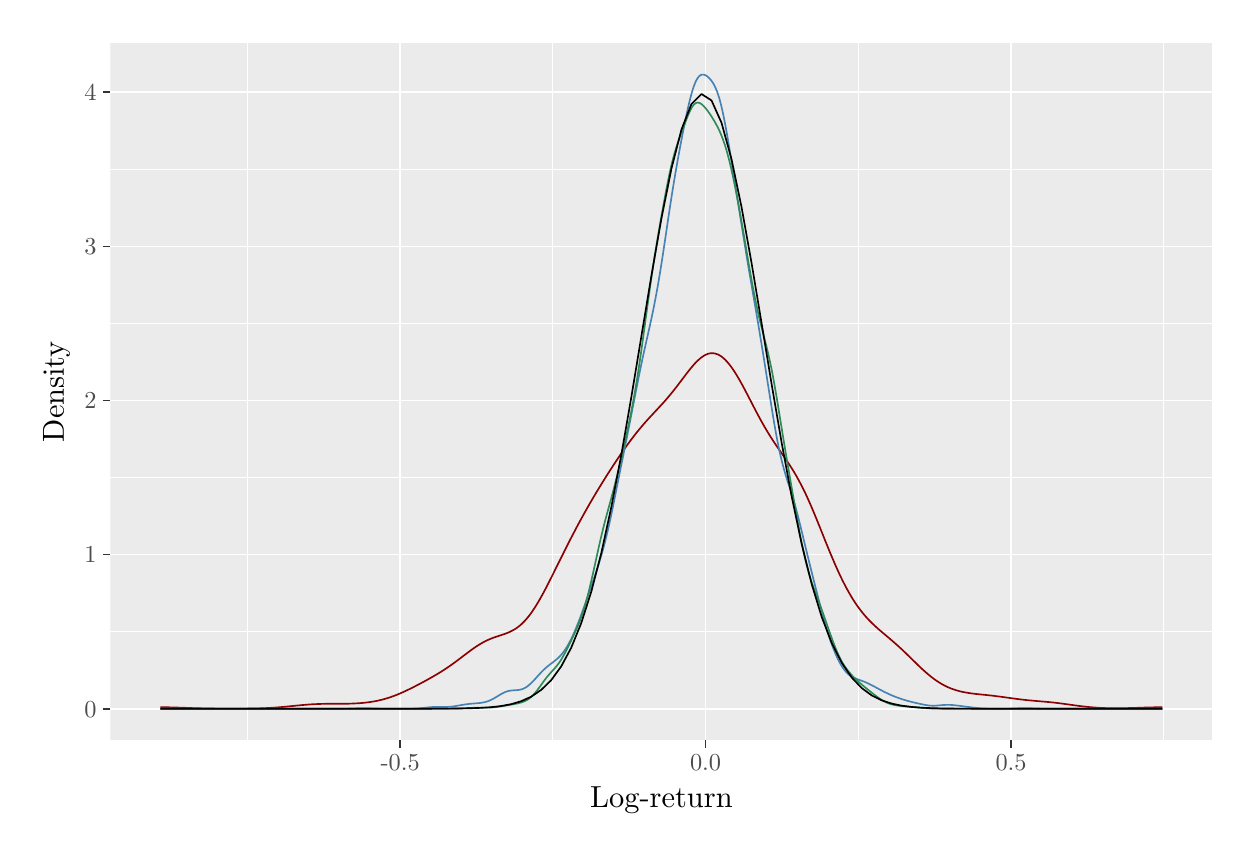
\begin{tikzpicture}[x=1pt,y=1pt]
\definecolor{fillColor}{RGB}{255,255,255}
\path[use as bounding box,fill=fillColor,fill opacity=0.00] (0,0) rectangle (433.62,289.08);
\begin{scope}
\path[clip] (  0.00,  0.00) rectangle (433.62,289.08);
\definecolor{drawColor}{RGB}{255,255,255}
\definecolor{fillColor}{RGB}{255,255,255}

\path[draw=drawColor,line width= 0.6pt,line join=round,line cap=round,fill=fillColor] (  0.00,  0.00) rectangle (433.62,289.08);
\end{scope}
\begin{scope}
\path[clip] ( 29.87, 31.53) rectangle (428.12,283.58);
\definecolor{fillColor}{gray}{0.92}

\path[fill=fillColor] ( 29.87, 31.53) rectangle (428.12,283.58);
\definecolor{drawColor}{RGB}{255,255,255}

\path[draw=drawColor,line width= 0.3pt,line join=round] ( 29.87, 70.83) --
	(428.12, 70.83);

\path[draw=drawColor,line width= 0.3pt,line join=round] ( 29.87,126.52) --
	(428.12,126.52);

\path[draw=drawColor,line width= 0.3pt,line join=round] ( 29.87,182.21) --
	(428.12,182.21);

\path[draw=drawColor,line width= 0.3pt,line join=round] ( 29.87,237.89) --
	(428.12,237.89);

\path[draw=drawColor,line width= 0.3pt,line join=round] ( 79.41, 31.53) --
	( 79.41,283.58);

\path[draw=drawColor,line width= 0.3pt,line join=round] (189.78, 31.53) --
	(189.78,283.58);

\path[draw=drawColor,line width= 0.3pt,line join=round] (300.16, 31.53) --
	(300.16,283.58);

\path[draw=drawColor,line width= 0.3pt,line join=round] (410.53, 31.53) --
	(410.53,283.58);

\path[draw=drawColor,line width= 0.6pt,line join=round] ( 29.87, 42.99) --
	(428.12, 42.99);

\path[draw=drawColor,line width= 0.6pt,line join=round] ( 29.87, 98.67) --
	(428.12, 98.67);

\path[draw=drawColor,line width= 0.6pt,line join=round] ( 29.87,154.36) --
	(428.12,154.36);

\path[draw=drawColor,line width= 0.6pt,line join=round] ( 29.87,210.05) --
	(428.12,210.05);

\path[draw=drawColor,line width= 0.6pt,line join=round] ( 29.87,265.74) --
	(428.12,265.74);

\path[draw=drawColor,line width= 0.6pt,line join=round] (134.60, 31.53) --
	(134.60,283.58);

\path[draw=drawColor,line width= 0.6pt,line join=round] (244.97, 31.53) --
	(244.97,283.58);

\path[draw=drawColor,line width= 0.6pt,line join=round] (355.35, 31.53) --
	(355.35,283.58);
\definecolor{drawColor}{RGB}{139,0,0}

\path[draw=drawColor,line width= 0.6pt,line join=round] ( 47.97, 43.52) --
	( 48.68, 43.52) --
	( 49.39, 43.51) --
	( 50.10, 43.50) --
	( 50.81, 43.49) --
	( 51.51, 43.48) --
	( 52.22, 43.46) --
	( 52.93, 43.44) --
	( 53.64, 43.42) --
	( 54.35, 43.40) --
	( 55.06, 43.37) --
	( 55.76, 43.35) --
	( 56.47, 43.32) --
	( 57.18, 43.30) --
	( 57.89, 43.27) --
	( 58.60, 43.25) --
	( 59.31, 43.22) --
	( 60.02, 43.20) --
	( 60.72, 43.18) --
	( 61.43, 43.16) --
	( 62.14, 43.14) --
	( 62.85, 43.12) --
	( 63.56, 43.10) --
	( 64.27, 43.09) --
	( 64.98, 43.07) --
	( 65.68, 43.06) --
	( 66.39, 43.05) --
	( 67.10, 43.04) --
	( 67.81, 43.03) --
	( 68.52, 43.02) --
	( 69.23, 43.02) --
	( 69.93, 43.01) --
	( 70.64, 43.01) --
	( 71.35, 43.01) --
	( 72.06, 43.00) --
	( 72.77, 43.00) --
	( 73.48, 43.00) --
	( 74.19, 43.00) --
	( 74.89, 43.00) --
	( 75.60, 43.00) --
	( 76.31, 43.01) --
	( 77.02, 43.01) --
	( 77.73, 43.01) --
	( 78.44, 43.02) --
	( 79.15, 43.03) --
	( 79.85, 43.04) --
	( 80.56, 43.05) --
	( 81.27, 43.06) --
	( 81.98, 43.07) --
	( 82.69, 43.09) --
	( 83.40, 43.11) --
	( 84.10, 43.13) --
	( 84.81, 43.15) --
	( 85.52, 43.18) --
	( 86.23, 43.21) --
	( 86.94, 43.25) --
	( 87.65, 43.29) --
	( 88.36, 43.33) --
	( 89.06, 43.37) --
	( 89.77, 43.42) --
	( 90.48, 43.48) --
	( 91.19, 43.54) --
	( 91.90, 43.60) --
	( 92.61, 43.66) --
	( 93.32, 43.73) --
	( 94.02, 43.80) --
	( 94.73, 43.87) --
	( 95.44, 43.94) --
	( 96.15, 44.01) --
	( 96.86, 44.08) --
	( 97.57, 44.15) --
	( 98.28, 44.22) --
	( 98.98, 44.29) --
	( 99.69, 44.35) --
	(100.40, 44.41) --
	(101.11, 44.47) --
	(101.82, 44.52) --
	(102.53, 44.57) --
	(103.23, 44.61) --
	(103.94, 44.64) --
	(104.65, 44.67) --
	(105.36, 44.70) --
	(106.07, 44.72) --
	(106.78, 44.74) --
	(107.49, 44.75) --
	(108.19, 44.75) --
	(108.90, 44.76) --
	(109.61, 44.76) --
	(110.32, 44.76) --
	(111.03, 44.76) --
	(111.74, 44.76) --
	(112.45, 44.76) --
	(113.15, 44.76) --
	(113.86, 44.77) --
	(114.57, 44.78) --
	(115.28, 44.79) --
	(115.99, 44.80) --
	(116.70, 44.82) --
	(117.40, 44.85) --
	(118.11, 44.88) --
	(118.82, 44.92) --
	(119.53, 44.96) --
	(120.24, 45.01) --
	(120.95, 45.07) --
	(121.66, 45.14) --
	(122.36, 45.22) --
	(123.07, 45.31) --
	(123.78, 45.41) --
	(124.49, 45.52) --
	(125.20, 45.64) --
	(125.91, 45.77) --
	(126.62, 45.92) --
	(127.32, 46.08) --
	(128.03, 46.25) --
	(128.74, 46.44) --
	(129.45, 46.64) --
	(130.16, 46.86) --
	(130.87, 47.09) --
	(131.57, 47.33) --
	(132.28, 47.59) --
	(132.99, 47.86) --
	(133.70, 48.14) --
	(134.41, 48.44) --
	(135.12, 48.75) --
	(135.83, 49.07) --
	(136.53, 49.39) --
	(137.24, 49.73) --
	(137.95, 50.07) --
	(138.66, 50.42) --
	(139.37, 50.78) --
	(140.08, 51.14) --
	(140.79, 51.51) --
	(141.49, 51.88) --
	(142.20, 52.25) --
	(142.91, 52.63) --
	(143.62, 53.02) --
	(144.33, 53.40) --
	(145.04, 53.80) --
	(145.74, 54.19) --
	(146.45, 54.60) --
	(147.16, 55.01) --
	(147.87, 55.43) --
	(148.58, 55.85) --
	(149.29, 56.29) --
	(150.00, 56.74) --
	(150.70, 57.20) --
	(151.41, 57.67) --
	(152.12, 58.15) --
	(152.83, 58.64) --
	(153.54, 59.14) --
	(154.25, 59.66) --
	(154.96, 60.18) --
	(155.66, 60.71) --
	(156.37, 61.25) --
	(157.08, 61.79) --
	(157.79, 62.33) --
	(158.50, 62.86) --
	(159.21, 63.40) --
	(159.92, 63.92) --
	(160.62, 64.44) --
	(161.33, 64.94) --
	(162.04, 65.42) --
	(162.75, 65.88) --
	(163.46, 66.32) --
	(164.17, 66.74) --
	(164.87, 67.12) --
	(165.58, 67.48) --
	(166.29, 67.82) --
	(167.00, 68.13) --
	(167.71, 68.42) --
	(168.42, 68.69) --
	(169.13, 68.93) --
	(169.83, 69.17) --
	(170.54, 69.40) --
	(171.25, 69.64) --
	(171.96, 69.87) --
	(172.67, 70.12) --
	(173.38, 70.39) --
	(174.09, 70.70) --
	(174.79, 71.03) --
	(175.50, 71.41) --
	(176.21, 71.83) --
	(176.92, 72.31) --
	(177.63, 72.85) --
	(178.34, 73.46) --
	(179.04, 74.13) --
	(179.75, 74.87) --
	(180.46, 75.68) --
	(181.17, 76.55) --
	(181.88, 77.50) --
	(182.59, 78.52) --
	(183.30, 79.60) --
	(184.00, 80.73) --
	(184.71, 81.92) --
	(185.42, 83.15) --
	(186.13, 84.44) --
	(186.84, 85.76) --
	(187.55, 87.12) --
	(188.26, 88.50) --
	(188.96, 89.90) --
	(189.67, 91.31) --
	(190.38, 92.74) --
	(191.09, 94.18) --
	(191.80, 95.61) --
	(192.51, 97.04) --
	(193.21, 98.47) --
	(193.92, 99.89) --
	(194.63,101.31) --
	(195.34,102.70) --
	(196.05,104.09) --
	(196.76,105.47) --
	(197.47,106.82) --
	(198.17,108.17) --
	(198.88,109.50) --
	(199.59,110.81) --
	(200.30,112.10) --
	(201.01,113.39) --
	(201.72,114.65) --
	(202.43,115.90) --
	(203.13,117.14) --
	(203.84,118.36) --
	(204.55,119.56) --
	(205.26,120.76) --
	(205.97,121.94) --
	(206.68,123.10) --
	(207.39,124.26) --
	(208.09,125.40) --
	(208.80,126.53) --
	(209.51,127.65) --
	(210.22,128.76) --
	(210.93,129.86) --
	(211.64,130.95) --
	(212.34,132.02) --
	(213.05,133.09) --
	(213.76,134.14) --
	(214.47,135.18) --
	(215.18,136.20) --
	(215.89,137.21) --
	(216.60,138.20) --
	(217.30,139.18) --
	(218.01,140.13) --
	(218.72,141.07) --
	(219.43,141.99) --
	(220.14,142.88) --
	(220.85,143.76) --
	(221.56,144.61) --
	(222.26,145.44) --
	(222.97,146.26) --
	(223.68,147.05) --
	(224.39,147.84) --
	(225.10,148.61) --
	(225.81,149.37) --
	(226.51,150.13) --
	(227.22,150.88) --
	(227.93,151.64) --
	(228.64,152.41) --
	(229.35,153.18) --
	(230.06,153.97) --
	(230.77,154.78) --
	(231.47,155.60) --
	(232.18,156.45) --
	(232.89,157.31) --
	(233.60,158.20) --
	(234.31,159.10) --
	(235.02,160.02) --
	(235.73,160.96) --
	(236.43,161.89) --
	(237.14,162.83) --
	(237.85,163.77) --
	(238.56,164.69) --
	(239.27,165.58) --
	(239.98,166.44) --
	(240.68,167.27) --
	(241.39,168.05) --
	(242.10,168.76) --
	(242.81,169.40) --
	(243.52,169.97) --
	(244.23,170.45) --
	(244.94,170.85) --
	(245.64,171.16) --
	(246.35,171.37) --
	(247.06,171.45) --
	(247.77,171.43) --
	(248.48,171.31) --
	(249.19,171.08) --
	(249.90,170.75) --
	(250.60,170.32) --
	(251.31,169.76) --
	(252.02,169.11) --
	(252.73,168.36) --
	(253.44,167.52) --
	(254.15,166.61) --
	(254.85,165.61) --
	(255.56,164.53) --
	(256.27,163.39) --
	(256.98,162.19) --
	(257.69,160.94) --
	(258.40,159.65) --
	(259.11,158.33) --
	(259.81,156.98) --
	(260.52,155.61) --
	(261.23,154.24) --
	(261.94,152.87) --
	(262.65,151.50) --
	(263.36,150.14) --
	(264.07,148.81) --
	(264.77,147.50) --
	(265.48,146.23) --
	(266.19,144.98) --
	(266.90,143.77) --
	(267.61,142.59) --
	(268.32,141.45) --
	(269.03,140.34) --
	(269.73,139.26) --
	(270.44,138.20) --
	(271.15,137.16) --
	(271.86,136.14) --
	(272.57,135.12) --
	(273.28,134.10) --
	(273.98,133.07) --
	(274.69,132.02) --
	(275.40,130.94) --
	(276.11,129.84) --
	(276.82,128.69) --
	(277.53,127.49) --
	(278.24,126.24) --
	(278.94,124.94) --
	(279.65,123.58) --
	(280.36,122.17) --
	(281.07,120.70) --
	(281.78,119.17) --
	(282.49,117.58) --
	(283.20,115.96) --
	(283.90,114.29) --
	(284.61,112.59) --
	(285.32,110.85) --
	(286.03,109.10) --
	(286.74,107.33) --
	(287.45,105.56) --
	(288.15,103.79) --
	(288.86,102.04) --
	(289.57,100.30) --
	(290.28, 98.59) --
	(290.99, 96.91) --
	(291.70, 95.27) --
	(292.41, 93.66) --
	(293.11, 92.11) --
	(293.82, 90.60) --
	(294.53, 89.15) --
	(295.24, 87.76) --
	(295.95, 86.42) --
	(296.66, 85.14) --
	(297.37, 83.91) --
	(298.07, 82.74) --
	(298.78, 81.63) --
	(299.49, 80.58) --
	(300.20, 79.58) --
	(300.91, 78.63) --
	(301.62, 77.72) --
	(302.32, 76.87) --
	(303.03, 76.06) --
	(303.74, 75.29) --
	(304.45, 74.55) --
	(305.16, 73.85) --
	(305.87, 73.17) --
	(306.58, 72.52) --
	(307.28, 71.88) --
	(307.99, 71.27) --
	(308.70, 70.66) --
	(309.41, 70.06) --
	(310.12, 69.47) --
	(310.83, 68.87) --
	(311.54, 68.27) --
	(312.24, 67.67) --
	(312.95, 67.05) --
	(313.66, 66.43) --
	(314.37, 65.80) --
	(315.08, 65.15) --
	(315.79, 64.50) --
	(316.49, 63.83) --
	(317.20, 63.15) --
	(317.91, 62.46) --
	(318.62, 61.77) --
	(319.33, 61.08) --
	(320.04, 60.38) --
	(320.75, 59.69) --
	(321.45, 59.00) --
	(322.16, 58.32) --
	(322.87, 57.65) --
	(323.58, 57.00) --
	(324.29, 56.36) --
	(325.00, 55.74) --
	(325.71, 55.15) --
	(326.41, 54.57) --
	(327.12, 54.02) --
	(327.83, 53.50) --
	(328.54, 53.01) --
	(329.25, 52.54) --
	(329.96, 52.11) --
	(330.67, 51.70) --
	(331.37, 51.33) --
	(332.08, 50.98) --
	(332.79, 50.65) --
	(333.50, 50.36) --
	(334.21, 50.09) --
	(334.92, 49.85) --
	(335.62, 49.63) --
	(336.33, 49.42) --
	(337.04, 49.24) --
	(337.75, 49.08) --
	(338.46, 48.94) --
	(339.17, 48.81) --
	(339.88, 48.69) --
	(340.58, 48.58) --
	(341.29, 48.48) --
	(342.00, 48.40) --
	(342.71, 48.31) --
	(343.42, 48.24) --
	(344.13, 48.16) --
	(344.84, 48.09) --
	(345.54, 48.02) --
	(346.25, 47.95) --
	(346.96, 47.87) --
	(347.67, 47.80) --
	(348.38, 47.72) --
	(349.09, 47.64) --
	(349.79, 47.55) --
	(350.50, 47.46) --
	(351.21, 47.37) --
	(351.92, 47.28) --
	(352.63, 47.18) --
	(353.34, 47.08) --
	(354.05, 46.98) --
	(354.75, 46.88) --
	(355.46, 46.78) --
	(356.17, 46.69) --
	(356.88, 46.59) --
	(357.59, 46.50) --
	(358.30, 46.41) --
	(359.01, 46.32) --
	(359.71, 46.24) --
	(360.42, 46.16) --
	(361.13, 46.09) --
	(361.84, 46.02) --
	(362.55, 45.95) --
	(363.26, 45.89) --
	(363.96, 45.82) --
	(364.67, 45.76) --
	(365.38, 45.70) --
	(366.09, 45.64) --
	(366.80, 45.58) --
	(367.51, 45.52) --
	(368.22, 45.46) --
	(368.92, 45.39) --
	(369.63, 45.32) --
	(370.34, 45.25) --
	(371.05, 45.17) --
	(371.76, 45.09) --
	(372.47, 45.00) --
	(373.18, 44.91) --
	(373.88, 44.82) --
	(374.59, 44.72) --
	(375.30, 44.63) --
	(376.01, 44.53) --
	(376.72, 44.43) --
	(377.43, 44.33) --
	(378.13, 44.23) --
	(378.84, 44.14) --
	(379.55, 44.04) --
	(380.26, 43.95) --
	(380.97, 43.86) --
	(381.68, 43.78) --
	(382.39, 43.70) --
	(383.09, 43.63) --
	(383.80, 43.56) --
	(384.51, 43.50) --
	(385.22, 43.44) --
	(385.93, 43.39) --
	(386.64, 43.34) --
	(387.35, 43.30) --
	(388.05, 43.26) --
	(388.76, 43.23) --
	(389.47, 43.21) --
	(390.18, 43.19) --
	(390.89, 43.17) --
	(391.60, 43.16) --
	(392.31, 43.15) --
	(393.01, 43.15) --
	(393.72, 43.15) --
	(394.43, 43.15) --
	(395.14, 43.16) --
	(395.85, 43.17) --
	(396.56, 43.18) --
	(397.26, 43.20) --
	(397.97, 43.22) --
	(398.68, 43.24) --
	(399.39, 43.26) --
	(400.10, 43.28) --
	(400.81, 43.30) --
	(401.52, 43.33) --
	(402.22, 43.35) --
	(402.93, 43.38) --
	(403.64, 43.40) --
	(404.35, 43.42) --
	(405.06, 43.44) --
	(405.77, 43.46) --
	(406.48, 43.48) --
	(407.18, 43.49) --
	(407.89, 43.50) --
	(408.60, 43.51) --
	(409.31, 43.52) --
	(410.02, 43.52);
\definecolor{drawColor}{RGB}{70,130,180}

\path[draw=drawColor,line width= 0.6pt,line join=round] ( 47.97, 42.99) --
	( 48.68, 42.99) --
	( 49.39, 42.99) --
	( 50.10, 42.99) --
	( 50.81, 42.99) --
	( 51.51, 42.99) --
	( 52.22, 42.99) --
	( 52.93, 42.99) --
	( 53.64, 42.99) --
	( 54.35, 42.99) --
	( 55.06, 42.99) --
	( 55.76, 42.99) --
	( 56.47, 42.99) --
	( 57.18, 42.99) --
	( 57.89, 42.99) --
	( 58.60, 42.99) --
	( 59.31, 42.99) --
	( 60.02, 42.99) --
	( 60.72, 42.99) --
	( 61.43, 42.99) --
	( 62.14, 42.99) --
	( 62.85, 42.99) --
	( 63.56, 42.99) --
	( 64.27, 42.99) --
	( 64.98, 42.99) --
	( 65.68, 42.99) --
	( 66.39, 42.99) --
	( 67.10, 42.99) --
	( 67.81, 42.99) --
	( 68.52, 42.99) --
	( 69.23, 42.99) --
	( 69.93, 42.99) --
	( 70.64, 42.99) --
	( 71.35, 42.99) --
	( 72.06, 42.99) --
	( 72.77, 42.99) --
	( 73.48, 42.99) --
	( 74.19, 42.99) --
	( 74.89, 42.99) --
	( 75.60, 42.99) --
	( 76.31, 42.99) --
	( 77.02, 42.99) --
	( 77.73, 42.99) --
	( 78.44, 42.99) --
	( 79.15, 42.99) --
	( 79.85, 42.99) --
	( 80.56, 42.99) --
	( 81.27, 42.99) --
	( 81.98, 42.99) --
	( 82.69, 42.99) --
	( 83.40, 42.99) --
	( 84.10, 42.99) --
	( 84.81, 42.99) --
	( 85.52, 42.99) --
	( 86.23, 42.99) --
	( 86.94, 42.99) --
	( 87.65, 42.99) --
	( 88.36, 42.99) --
	( 89.06, 42.99) --
	( 89.77, 42.99) --
	( 90.48, 42.99) --
	( 91.19, 42.99) --
	( 91.90, 42.99) --
	( 92.61, 42.99) --
	( 93.32, 42.99) --
	( 94.02, 42.99) --
	( 94.73, 42.99) --
	( 95.44, 42.99) --
	( 96.15, 42.99) --
	( 96.86, 42.99) --
	( 97.57, 42.99) --
	( 98.28, 42.99) --
	( 98.98, 42.99) --
	( 99.69, 42.99) --
	(100.40, 42.99) --
	(101.11, 42.99) --
	(101.82, 42.99) --
	(102.53, 42.99) --
	(103.23, 42.99) --
	(103.94, 42.99) --
	(104.65, 42.99) --
	(105.36, 42.99) --
	(106.07, 42.99) --
	(106.78, 42.99) --
	(107.49, 42.99) --
	(108.19, 42.99) --
	(108.90, 42.99) --
	(109.61, 42.99) --
	(110.32, 42.99) --
	(111.03, 42.99) --
	(111.74, 42.99) --
	(112.45, 42.99) --
	(113.15, 43.00) --
	(113.86, 43.00) --
	(114.57, 43.01) --
	(115.28, 43.02) --
	(115.99, 43.04) --
	(116.70, 43.06) --
	(117.40, 43.08) --
	(118.11, 43.10) --
	(118.82, 43.13) --
	(119.53, 43.15) --
	(120.24, 43.17) --
	(120.95, 43.17) --
	(121.66, 43.18) --
	(122.36, 43.17) --
	(123.07, 43.15) --
	(123.78, 43.13) --
	(124.49, 43.11) --
	(125.20, 43.08) --
	(125.91, 43.06) --
	(126.62, 43.04) --
	(127.32, 43.02) --
	(128.03, 43.01) --
	(128.74, 43.00) --
	(129.45, 43.00) --
	(130.16, 42.99) --
	(130.87, 42.99) --
	(131.57, 42.99) --
	(132.28, 42.99) --
	(132.99, 42.99) --
	(133.70, 42.99) --
	(134.41, 42.99) --
	(135.12, 42.99) --
	(135.83, 42.99) --
	(136.53, 42.99) --
	(137.24, 43.00) --
	(137.95, 43.00) --
	(138.66, 43.01) --
	(139.37, 43.03) --
	(140.08, 43.06) --
	(140.79, 43.09) --
	(141.49, 43.14) --
	(142.20, 43.20) --
	(142.91, 43.27) --
	(143.62, 43.34) --
	(144.33, 43.42) --
	(145.04, 43.49) --
	(145.74, 43.55) --
	(146.45, 43.60) --
	(147.16, 43.62) --
	(147.87, 43.63) --
	(148.58, 43.62) --
	(149.29, 43.61) --
	(150.00, 43.60) --
	(150.70, 43.60) --
	(151.41, 43.61) --
	(152.12, 43.65) --
	(152.83, 43.70) --
	(153.54, 43.78) --
	(154.25, 43.88) --
	(154.96, 44.00) --
	(155.66, 44.12) --
	(156.37, 44.25) --
	(157.08, 44.37) --
	(157.79, 44.49) --
	(158.50, 44.59) --
	(159.21, 44.68) --
	(159.92, 44.76) --
	(160.62, 44.82) --
	(161.33, 44.88) --
	(162.04, 44.93) --
	(162.75, 44.99) --
	(163.46, 45.06) --
	(164.17, 45.16) --
	(164.87, 45.30) --
	(165.58, 45.47) --
	(166.29, 45.70) --
	(167.00, 45.98) --
	(167.71, 46.32) --
	(168.42, 46.69) --
	(169.13, 47.10) --
	(169.83, 47.53) --
	(170.54, 47.96) --
	(171.25, 48.37) --
	(171.96, 48.74) --
	(172.67, 49.05) --
	(173.38, 49.29) --
	(174.09, 49.46) --
	(174.79, 49.57) --
	(175.50, 49.63) --
	(176.21, 49.67) --
	(176.92, 49.71) --
	(177.63, 49.79) --
	(178.34, 49.95) --
	(179.04, 50.19) --
	(179.75, 50.53) --
	(180.46, 50.99) --
	(181.17, 51.54) --
	(181.88, 52.18) --
	(182.59, 52.89) --
	(183.30, 53.65) --
	(184.00, 54.43) --
	(184.71, 55.21) --
	(185.42, 55.98) --
	(186.13, 56.71) --
	(186.84, 57.39) --
	(187.55, 58.02) --
	(188.26, 58.60) --
	(188.96, 59.15) --
	(189.67, 59.68) --
	(190.38, 60.23) --
	(191.09, 60.80) --
	(191.80, 61.43) --
	(192.51, 62.15) --
	(193.21, 62.97) --
	(193.92, 63.90) --
	(194.63, 64.96) --
	(195.34, 66.16) --
	(196.05, 67.48) --
	(196.76, 68.91) --
	(197.47, 70.47) --
	(198.17, 72.13) --
	(198.88, 73.89) --
	(199.59, 75.74) --
	(200.30, 77.66) --
	(201.01, 79.63) --
	(201.72, 81.64) --
	(202.43, 83.68) --
	(203.13, 85.72) --
	(203.84, 87.77) --
	(204.55, 89.84) --
	(205.26, 91.94) --
	(205.97, 94.10) --
	(206.68, 96.35) --
	(207.39, 98.72) --
	(208.09,101.25) --
	(208.80,103.97) --
	(209.51,106.90) --
	(210.22,110.01) --
	(210.93,113.30) --
	(211.64,116.73) --
	(212.34,120.24) --
	(213.05,123.80) --
	(213.76,127.36) --
	(214.47,130.89) --
	(215.18,134.40) --
	(215.89,137.90) --
	(216.60,141.42) --
	(217.30,144.98) --
	(218.01,148.59) --
	(218.72,152.25) --
	(219.43,155.92) --
	(220.14,159.56) --
	(220.85,163.12) --
	(221.56,166.57) --
	(222.26,169.91) --
	(222.97,173.14) --
	(223.68,176.30) --
	(224.39,179.44) --
	(225.10,182.63) --
	(225.81,185.94) --
	(226.51,189.44) --
	(227.22,193.16) --
	(227.93,197.16) --
	(228.64,201.43) --
	(229.35,205.94) --
	(230.06,210.64) --
	(230.77,215.42) --
	(231.47,220.19) --
	(232.18,224.88) --
	(232.89,229.43) --
	(233.60,233.80) --
	(234.31,237.97) --
	(235.02,241.98) --
	(235.73,245.83) --
	(236.43,249.55) --
	(237.14,253.15) --
	(237.85,256.62) --
	(238.56,259.90) --
	(239.27,262.93) --
	(239.98,265.61) --
	(240.68,267.85) --
	(241.39,269.62) --
	(242.10,270.90) --
	(242.81,271.71) --
	(243.52,272.09) --
	(244.23,272.12) --
	(244.94,271.88) --
	(245.64,271.42) --
	(246.35,270.77) --
	(247.06,269.94) --
	(247.77,268.88) --
	(248.48,267.53) --
	(249.19,265.81) --
	(249.90,263.66) --
	(250.60,260.99) --
	(251.31,257.86) --
	(252.02,254.30) --
	(252.73,250.39) --
	(253.44,246.23) --
	(254.15,241.90) --
	(254.85,237.48) --
	(255.56,233.00) --
	(256.27,228.50) --
	(256.98,224.01) --
	(257.69,219.54) --
	(258.40,215.10) --
	(259.11,210.72) --
	(259.81,206.40) --
	(260.52,202.17) --
	(261.23,198.01) --
	(261.94,193.89) --
	(262.65,189.78) --
	(263.36,185.65) --
	(264.07,181.47) --
	(264.77,177.22) --
	(265.48,172.89) --
	(266.19,168.48) --
	(266.90,164.00) --
	(267.61,159.49) --
	(268.32,155.00) --
	(269.03,150.57) --
	(269.73,146.30) --
	(270.44,142.25) --
	(271.15,138.52) --
	(271.86,135.17) --
	(272.57,132.18) --
	(273.28,129.52) --
	(273.98,127.12) --
	(274.69,124.88) --
	(275.40,122.70) --
	(276.11,120.47) --
	(276.82,118.12) --
	(277.53,115.62) --
	(278.24,112.96) --
	(278.94,110.17) --
	(279.65,107.27) --
	(280.36,104.33) --
	(281.07,101.39) --
	(281.78, 98.47) --
	(282.49, 95.59) --
	(283.20, 92.75) --
	(283.90, 89.94) --
	(284.61, 87.14) --
	(285.32, 84.36) --
	(286.03, 81.62) --
	(286.74, 78.92) --
	(287.45, 76.30) --
	(288.15, 73.78) --
	(288.86, 71.38) --
	(289.57, 69.13) --
	(290.28, 67.03) --
	(290.99, 65.09) --
	(291.70, 63.31) --
	(292.41, 61.69) --
	(293.11, 60.23) --
	(293.82, 58.93) --
	(294.53, 57.79) --
	(295.24, 56.82) --
	(295.95, 56.01) --
	(296.66, 55.34) --
	(297.37, 54.81) --
	(298.07, 54.38) --
	(298.78, 54.04) --
	(299.49, 53.75) --
	(300.20, 53.50) --
	(300.91, 53.25) --
	(301.62, 52.99) --
	(302.32, 52.72) --
	(303.03, 52.42) --
	(303.74, 52.09) --
	(304.45, 51.75) --
	(305.16, 51.39) --
	(305.87, 51.02) --
	(306.58, 50.64) --
	(307.28, 50.26) --
	(307.99, 49.88) --
	(308.70, 49.51) --
	(309.41, 49.14) --
	(310.12, 48.79) --
	(310.83, 48.45) --
	(311.54, 48.12) --
	(312.24, 47.81) --
	(312.95, 47.52) --
	(313.66, 47.24) --
	(314.37, 46.98) --
	(315.08, 46.73) --
	(315.79, 46.49) --
	(316.49, 46.26) --
	(317.20, 46.05) --
	(317.91, 45.84) --
	(318.62, 45.64) --
	(319.33, 45.46) --
	(320.04, 45.29) --
	(320.75, 45.12) --
	(321.45, 44.96) --
	(322.16, 44.80) --
	(322.87, 44.65) --
	(323.58, 44.50) --
	(324.29, 44.36) --
	(325.00, 44.24) --
	(325.71, 44.15) --
	(326.41, 44.09) --
	(327.12, 44.07) --
	(327.83, 44.08) --
	(328.54, 44.12) --
	(329.25, 44.18) --
	(329.96, 44.25) --
	(330.67, 44.31) --
	(331.37, 44.35) --
	(332.08, 44.38) --
	(332.79, 44.38) --
	(333.50, 44.36) --
	(334.21, 44.31) --
	(334.92, 44.24) --
	(335.62, 44.16) --
	(336.33, 44.08) --
	(337.04, 43.99) --
	(337.75, 43.90) --
	(338.46, 43.80) --
	(339.17, 43.71) --
	(339.88, 43.62) --
	(340.58, 43.53) --
	(341.29, 43.44) --
	(342.00, 43.36) --
	(342.71, 43.28) --
	(343.42, 43.21) --
	(344.13, 43.15) --
	(344.84, 43.10) --
	(345.54, 43.07) --
	(346.25, 43.04) --
	(346.96, 43.02) --
	(347.67, 43.01) --
	(348.38, 43.00) --
	(349.09, 42.99) --
	(349.79, 42.99) --
	(350.50, 42.99) --
	(351.21, 42.99) --
	(351.92, 43.00) --
	(352.63, 43.00) --
	(353.34, 43.01) --
	(354.05, 43.02) --
	(354.75, 43.03) --
	(355.46, 43.05) --
	(356.17, 43.07) --
	(356.88, 43.10) --
	(357.59, 43.12) --
	(358.30, 43.14) --
	(359.01, 43.16) --
	(359.71, 43.17) --
	(360.42, 43.18) --
	(361.13, 43.17) --
	(361.84, 43.16) --
	(362.55, 43.14) --
	(363.26, 43.12) --
	(363.96, 43.09) --
	(364.67, 43.07) --
	(365.38, 43.05) --
	(366.09, 43.03) --
	(366.80, 43.02) --
	(367.51, 43.01) --
	(368.22, 43.00) --
	(368.92, 42.99) --
	(369.63, 42.99) --
	(370.34, 42.99) --
	(371.05, 42.99) --
	(371.76, 42.99) --
	(372.47, 42.99) --
	(373.18, 42.99) --
	(373.88, 42.99) --
	(374.59, 42.99) --
	(375.30, 42.99) --
	(376.01, 42.99) --
	(376.72, 42.99) --
	(377.43, 42.99) --
	(378.13, 42.99) --
	(378.84, 42.99) --
	(379.55, 42.99) --
	(380.26, 42.99) --
	(380.97, 42.99) --
	(381.68, 42.99) --
	(382.39, 42.99) --
	(383.09, 42.99) --
	(383.80, 42.99) --
	(384.51, 42.99) --
	(385.22, 42.99) --
	(385.93, 42.99) --
	(386.64, 42.99) --
	(387.35, 42.99) --
	(388.05, 42.99) --
	(388.76, 42.99) --
	(389.47, 42.99) --
	(390.18, 42.99) --
	(390.89, 42.99) --
	(391.60, 42.99) --
	(392.31, 42.99) --
	(393.01, 42.99) --
	(393.72, 42.99) --
	(394.43, 42.99) --
	(395.14, 42.99) --
	(395.85, 42.99) --
	(396.56, 42.99) --
	(397.26, 42.99) --
	(397.97, 42.99) --
	(398.68, 42.99) --
	(399.39, 42.99) --
	(400.10, 42.99) --
	(400.81, 42.99) --
	(401.52, 42.99) --
	(402.22, 42.99) --
	(402.93, 42.99) --
	(403.64, 42.99) --
	(404.35, 42.99) --
	(405.06, 42.99) --
	(405.77, 42.99) --
	(406.48, 42.99) --
	(407.18, 42.99) --
	(407.89, 42.99) --
	(408.60, 42.99) --
	(409.31, 42.99) --
	(410.02, 42.99);
\definecolor{drawColor}{RGB}{46,139,87}

\path[draw=drawColor,line width= 0.6pt,line join=round] ( 47.97, 42.99) --
	( 48.68, 42.99) --
	( 49.39, 42.99) --
	( 50.10, 42.99) --
	( 50.81, 42.99) --
	( 51.51, 42.99) --
	( 52.22, 42.99) --
	( 52.93, 42.99) --
	( 53.64, 42.99) --
	( 54.35, 42.99) --
	( 55.06, 42.99) --
	( 55.76, 42.99) --
	( 56.47, 42.99) --
	( 57.18, 42.99) --
	( 57.89, 42.99) --
	( 58.60, 42.99) --
	( 59.31, 42.99) --
	( 60.02, 42.99) --
	( 60.72, 42.99) --
	( 61.43, 42.99) --
	( 62.14, 42.99) --
	( 62.85, 42.99) --
	( 63.56, 42.99) --
	( 64.27, 42.99) --
	( 64.98, 42.99) --
	( 65.68, 42.99) --
	( 66.39, 42.99) --
	( 67.10, 42.99) --
	( 67.81, 42.99) --
	( 68.52, 42.99) --
	( 69.23, 42.99) --
	( 69.93, 42.99) --
	( 70.64, 42.99) --
	( 71.35, 42.99) --
	( 72.06, 42.99) --
	( 72.77, 42.99) --
	( 73.48, 42.99) --
	( 74.19, 42.99) --
	( 74.89, 42.99) --
	( 75.60, 42.99) --
	( 76.31, 42.99) --
	( 77.02, 42.99) --
	( 77.73, 42.99) --
	( 78.44, 42.99) --
	( 79.15, 42.99) --
	( 79.85, 42.99) --
	( 80.56, 42.99) --
	( 81.27, 42.99) --
	( 81.98, 42.99) --
	( 82.69, 42.99) --
	( 83.40, 42.99) --
	( 84.10, 42.99) --
	( 84.81, 42.99) --
	( 85.52, 42.99) --
	( 86.23, 42.99) --
	( 86.94, 42.99) --
	( 87.65, 42.99) --
	( 88.36, 42.99) --
	( 89.06, 42.99) --
	( 89.77, 42.99) --
	( 90.48, 42.99) --
	( 91.19, 42.99) --
	( 91.90, 42.99) --
	( 92.61, 42.99) --
	( 93.32, 42.99) --
	( 94.02, 42.99) --
	( 94.73, 42.99) --
	( 95.44, 42.99) --
	( 96.15, 42.99) --
	( 96.86, 42.99) --
	( 97.57, 42.99) --
	( 98.28, 42.99) --
	( 98.98, 42.99) --
	( 99.69, 42.99) --
	(100.40, 42.99) --
	(101.11, 42.99) --
	(101.82, 42.99) --
	(102.53, 42.99) --
	(103.23, 42.99) --
	(103.94, 42.99) --
	(104.65, 42.99) --
	(105.36, 42.99) --
	(106.07, 42.99) --
	(106.78, 42.99) --
	(107.49, 42.99) --
	(108.19, 42.99) --
	(108.90, 42.99) --
	(109.61, 42.99) --
	(110.32, 42.99) --
	(111.03, 42.99) --
	(111.74, 42.99) --
	(112.45, 42.99) --
	(113.15, 42.99) --
	(113.86, 42.99) --
	(114.57, 42.99) --
	(115.28, 42.99) --
	(115.99, 42.99) --
	(116.70, 42.99) --
	(117.40, 42.99) --
	(118.11, 42.99) --
	(118.82, 42.99) --
	(119.53, 42.99) --
	(120.24, 42.99) --
	(120.95, 42.99) --
	(121.66, 42.99) --
	(122.36, 42.99) --
	(123.07, 42.99) --
	(123.78, 42.99) --
	(124.49, 42.99) --
	(125.20, 42.99) --
	(125.91, 42.99) --
	(126.62, 42.99) --
	(127.32, 42.99) --
	(128.03, 42.99) --
	(128.74, 42.99) --
	(129.45, 42.99) --
	(130.16, 42.99) --
	(130.87, 42.99) --
	(131.57, 42.99) --
	(132.28, 42.99) --
	(132.99, 42.99) --
	(133.70, 42.99) --
	(134.41, 42.99) --
	(135.12, 42.99) --
	(135.83, 42.99) --
	(136.53, 42.99) --
	(137.24, 42.99) --
	(137.95, 42.99) --
	(138.66, 42.99) --
	(139.37, 42.99) --
	(140.08, 42.99) --
	(140.79, 42.99) --
	(141.49, 42.99) --
	(142.20, 42.99) --
	(142.91, 42.99) --
	(143.62, 42.99) --
	(144.33, 42.99) --
	(145.04, 42.99) --
	(145.74, 42.99) --
	(146.45, 42.99) --
	(147.16, 42.99) --
	(147.87, 42.99) --
	(148.58, 42.99) --
	(149.29, 42.99) --
	(150.00, 42.99) --
	(150.70, 42.99) --
	(151.41, 43.00) --
	(152.12, 43.00) --
	(152.83, 43.01) --
	(153.54, 43.03) --
	(154.25, 43.04) --
	(154.96, 43.06) --
	(155.66, 43.09) --
	(156.37, 43.12) --
	(157.08, 43.15) --
	(157.79, 43.18) --
	(158.50, 43.21) --
	(159.21, 43.24) --
	(159.92, 43.27) --
	(160.62, 43.30) --
	(161.33, 43.32) --
	(162.04, 43.34) --
	(162.75, 43.36) --
	(163.46, 43.37) --
	(164.17, 43.37) --
	(164.87, 43.37) --
	(165.58, 43.37) --
	(166.29, 43.38) --
	(167.00, 43.40) --
	(167.71, 43.43) --
	(168.42, 43.49) --
	(169.13, 43.56) --
	(169.83, 43.65) --
	(170.54, 43.76) --
	(171.25, 43.87) --
	(171.96, 43.99) --
	(172.67, 44.12) --
	(173.38, 44.24) --
	(174.09, 44.37) --
	(174.79, 44.49) --
	(175.50, 44.61) --
	(176.21, 44.74) --
	(176.92, 44.88) --
	(177.63, 45.04) --
	(178.34, 45.24) --
	(179.04, 45.48) --
	(179.75, 45.77) --
	(180.46, 46.15) --
	(181.17, 46.61) --
	(181.88, 47.17) --
	(182.59, 47.85) --
	(183.30, 48.62) --
	(184.00, 49.49) --
	(184.71, 50.44) --
	(185.42, 51.42) --
	(186.13, 52.42) --
	(186.84, 53.39) --
	(187.55, 54.31) --
	(188.26, 55.16) --
	(188.96, 55.96) --
	(189.67, 56.74) --
	(190.38, 57.52) --
	(191.09, 58.35) --
	(191.80, 59.26) --
	(192.51, 60.29) --
	(193.21, 61.43) --
	(193.92, 62.69) --
	(194.63, 64.03) --
	(195.34, 65.45) --
	(196.05, 66.90) --
	(196.76, 68.38) --
	(197.47, 69.89) --
	(198.17, 71.45) --
	(198.88, 73.10) --
	(199.59, 74.88) --
	(200.30, 76.84) --
	(201.01, 79.01) --
	(201.72, 81.42) --
	(202.43, 84.06) --
	(203.13, 86.92) --
	(203.84, 89.96) --
	(204.55, 93.13) --
	(205.26, 96.36) --
	(205.97, 99.60) --
	(206.68,102.76) --
	(207.39,105.81) --
	(208.09,108.69) --
	(208.80,111.44) --
	(209.51,114.07) --
	(210.22,116.65) --
	(210.93,119.23) --
	(211.64,121.86) --
	(212.34,124.58) --
	(213.05,127.42) --
	(213.76,130.36) --
	(214.47,133.40) --
	(215.18,136.52) --
	(215.89,139.71) --
	(216.60,142.98) --
	(217.30,146.35) --
	(218.01,149.86) --
	(218.72,153.57) --
	(219.43,157.53) --
	(220.14,161.77) --
	(220.85,166.31) --
	(221.56,171.12) --
	(222.26,176.15) --
	(222.97,181.33) --
	(223.68,186.56) --
	(224.39,191.73) --
	(225.10,196.75) --
	(225.81,201.57) --
	(226.51,206.17) --
	(227.22,210.56) --
	(227.93,214.78) --
	(228.64,218.87) --
	(229.35,222.87) --
	(230.06,226.77) --
	(230.77,230.55) --
	(231.47,234.14) --
	(232.18,237.48) --
	(232.89,240.50) --
	(233.60,243.20) --
	(234.31,245.60) --
	(235.02,247.75) --
	(235.73,249.75) --
	(236.43,251.67) --
	(237.14,253.56) --
	(237.85,255.44) --
	(238.56,257.25) --
	(239.27,258.89) --
	(239.98,260.26) --
	(240.68,261.25) --
	(241.39,261.83) --
	(242.10,262.02) --
	(242.81,261.87) --
	(243.52,261.43) --
	(244.23,260.79) --
	(244.94,260.00) --
	(245.64,259.10) --
	(246.35,258.12) --
	(247.06,257.06) --
	(247.77,255.93) --
	(248.48,254.71) --
	(249.19,253.40) --
	(249.90,251.96) --
	(250.60,250.35) --
	(251.31,248.52) --
	(252.02,246.42) --
	(252.73,244.05) --
	(253.44,241.39) --
	(254.15,238.45) --
	(254.85,235.27) --
	(255.56,231.86) --
	(256.27,228.24) --
	(256.98,224.45) --
	(257.69,220.50) --
	(258.40,216.43) --
	(259.11,212.26) --
	(259.81,208.06) --
	(260.52,203.88) --
	(261.23,199.79) --
	(261.94,195.86) --
	(262.65,192.15) --
	(263.36,188.69) --
	(264.07,185.47) --
	(264.77,182.48) --
	(265.48,179.65) --
	(266.19,176.89) --
	(266.90,174.10) --
	(267.61,171.17) --
	(268.32,168.00) --
	(269.03,164.52) --
	(269.73,160.73) --
	(270.44,156.66) --
	(271.15,152.39) --
	(271.86,148.01) --
	(272.57,143.61) --
	(273.28,139.28) --
	(273.98,135.03) --
	(274.69,130.85) --
	(275.40,126.73) --
	(276.11,122.63) --
	(276.82,118.55) --
	(277.53,114.49) --
	(278.24,110.51) --
	(278.94,106.66) --
	(279.65,103.01) --
	(280.36, 99.62) --
	(281.07, 96.52) --
	(281.78, 93.73) --
	(282.49, 91.23) --
	(283.20, 88.98) --
	(283.90, 86.92) --
	(284.61, 84.97) --
	(285.32, 83.08) --
	(286.03, 81.20) --
	(286.74, 79.29) --
	(287.45, 77.33) --
	(288.15, 75.33) --
	(288.86, 73.29) --
	(289.57, 71.25) --
	(290.28, 69.24) --
	(290.99, 67.29) --
	(291.70, 65.44) --
	(292.41, 63.72) --
	(293.11, 62.13) --
	(293.82, 60.71) --
	(294.53, 59.44) --
	(295.24, 58.31) --
	(295.95, 57.31) --
	(296.66, 56.40) --
	(297.37, 55.58) --
	(298.07, 54.81) --
	(298.78, 54.10) --
	(299.49, 53.41) --
	(300.20, 52.76) --
	(300.91, 52.13) --
	(301.62, 51.52) --
	(302.32, 50.93) --
	(303.03, 50.35) --
	(303.74, 49.78) --
	(304.45, 49.21) --
	(305.16, 48.66) --
	(305.87, 48.10) --
	(306.58, 47.57) --
	(307.28, 47.05) --
	(307.99, 46.56) --
	(308.70, 46.10) --
	(309.41, 45.70) --
	(310.12, 45.34) --
	(310.83, 45.03) --
	(311.54, 44.77) --
	(312.24, 44.56) --
	(312.95, 44.38) --
	(313.66, 44.24) --
	(314.37, 44.12) --
	(315.08, 44.03) --
	(315.79, 43.95) --
	(316.49, 43.88) --
	(317.20, 43.81) --
	(317.91, 43.75) --
	(318.62, 43.70) --
	(319.33, 43.64) --
	(320.04, 43.58) --
	(320.75, 43.52) --
	(321.45, 43.45) --
	(322.16, 43.39) --
	(322.87, 43.32) --
	(323.58, 43.26) --
	(324.29, 43.20) --
	(325.00, 43.15) --
	(325.71, 43.10) --
	(326.41, 43.07) --
	(327.12, 43.04) --
	(327.83, 43.02) --
	(328.54, 43.01) --
	(329.25, 43.00) --
	(329.96, 43.00) --
	(330.67, 42.99) --
	(331.37, 42.99) --
	(332.08, 42.99) --
	(332.79, 42.99) --
	(333.50, 42.99) --
	(334.21, 42.99) --
	(334.92, 42.99) --
	(335.62, 42.99) --
	(336.33, 42.99) --
	(337.04, 42.99) --
	(337.75, 42.99) --
	(338.46, 42.99) --
	(339.17, 42.99) --
	(339.88, 42.99) --
	(340.58, 42.99) --
	(341.29, 42.99) --
	(342.00, 42.99) --
	(342.71, 42.99) --
	(343.42, 42.99) --
	(344.13, 42.99) --
	(344.84, 42.99) --
	(345.54, 42.99) --
	(346.25, 42.99) --
	(346.96, 42.99) --
	(347.67, 42.99) --
	(348.38, 42.99) --
	(349.09, 42.99) --
	(349.79, 42.99) --
	(350.50, 42.99) --
	(351.21, 42.99) --
	(351.92, 42.99) --
	(352.63, 42.99) --
	(353.34, 42.99) --
	(354.05, 42.99) --
	(354.75, 42.99) --
	(355.46, 42.99) --
	(356.17, 42.99) --
	(356.88, 42.99) --
	(357.59, 42.99) --
	(358.30, 42.99) --
	(359.01, 42.99) --
	(359.71, 42.99) --
	(360.42, 42.99) --
	(361.13, 42.99) --
	(361.84, 42.99) --
	(362.55, 42.99) --
	(363.26, 42.99) --
	(363.96, 42.99) --
	(364.67, 42.99) --
	(365.38, 42.99) --
	(366.09, 42.99) --
	(366.80, 42.99) --
	(367.51, 42.99) --
	(368.22, 42.99) --
	(368.92, 42.99) --
	(369.63, 42.99) --
	(370.34, 42.99) --
	(371.05, 42.99) --
	(371.76, 42.99) --
	(372.47, 42.99) --
	(373.18, 42.99) --
	(373.88, 42.99) --
	(374.59, 42.99) --
	(375.30, 42.99) --
	(376.01, 42.99) --
	(376.72, 42.99) --
	(377.43, 42.99) --
	(378.13, 42.99) --
	(378.84, 42.99) --
	(379.55, 42.99) --
	(380.26, 42.99) --
	(380.97, 42.99) --
	(381.68, 42.99) --
	(382.39, 42.99) --
	(383.09, 42.99) --
	(383.80, 42.99) --
	(384.51, 42.99) --
	(385.22, 42.99) --
	(385.93, 42.99) --
	(386.64, 42.99) --
	(387.35, 42.99) --
	(388.05, 42.99) --
	(388.76, 42.99) --
	(389.47, 42.99) --
	(390.18, 42.99) --
	(390.89, 42.99) --
	(391.60, 42.99) --
	(392.31, 42.99) --
	(393.01, 42.99) --
	(393.72, 42.99) --
	(394.43, 42.99) --
	(395.14, 42.99) --
	(395.85, 42.99) --
	(396.56, 42.99) --
	(397.26, 42.99) --
	(397.97, 42.99) --
	(398.68, 42.99) --
	(399.39, 42.99) --
	(400.10, 42.99) --
	(400.81, 42.99) --
	(401.52, 42.99) --
	(402.22, 42.99) --
	(402.93, 42.99) --
	(403.64, 42.99) --
	(404.35, 42.99) --
	(405.06, 42.99) --
	(405.77, 42.99) --
	(406.48, 42.99) --
	(407.18, 42.99) --
	(407.89, 42.99) --
	(408.60, 42.99) --
	(409.31, 42.99) --
	(410.02, 42.99);
\definecolor{drawColor}{RGB}{0,0,0}

\path[draw=drawColor,line width= 0.6pt,line join=round] ( 47.97, 42.99) --
	( 51.59, 42.99) --
	( 55.21, 42.99) --
	( 58.83, 42.99) --
	( 62.45, 42.99) --
	( 66.07, 42.99) --
	( 69.69, 42.99) --
	( 73.31, 42.99) --
	( 76.93, 42.99) --
	( 80.56, 42.99) --
	( 84.18, 42.99) --
	( 87.80, 42.99) --
	( 91.42, 42.99) --
	( 95.04, 42.99) --
	( 98.66, 42.99) --
	(102.28, 42.99) --
	(105.90, 42.99) --
	(109.52, 42.99) --
	(113.14, 42.99) --
	(116.76, 42.99) --
	(120.38, 42.99) --
	(124.00, 42.99) --
	(127.62, 42.99) --
	(131.24, 42.99) --
	(134.86, 42.99) --
	(138.48, 42.99) --
	(142.10, 42.99) --
	(145.72, 43.00) --
	(149.34, 43.01) --
	(152.96, 43.03) --
	(156.59, 43.08) --
	(160.21, 43.16) --
	(163.83, 43.30) --
	(167.45, 43.54) --
	(171.07, 43.95) --
	(174.69, 44.62) --
	(178.31, 45.69) --
	(181.93, 47.32) --
	(185.55, 49.77) --
	(189.17, 53.30) --
	(192.79, 58.27) --
	(196.41, 65.02) --
	(200.03, 73.92) --
	(203.65, 85.25) --
	(207.27, 99.21) --
	(210.89,115.79) --
	(214.51,134.75) --
	(218.13,155.59) --
	(221.75,177.50) --
	(225.37,199.40) --
	(228.99,220.04) --
	(232.61,238.08) --
	(236.24,252.26) --
	(239.86,261.51) --
	(243.48,265.11) --
	(247.10,262.78) --
	(250.72,254.71) --
	(254.34,241.51) --
	(257.96,224.20) --
	(261.58,204.01) --
	(265.20,182.27) --
	(268.82,160.27) --
	(272.44,139.12) --
	(276.06,119.70) --
	(279.68,102.57) --
	(283.30, 88.04) --
	(286.92, 76.15) --
	(290.54, 66.75) --
	(294.16, 59.56) --
	(297.78, 54.24) --
	(301.40, 50.43) --
	(305.02, 47.77) --
	(308.64, 45.99) --
	(312.27, 44.82) --
	(315.89, 44.07) --
	(319.51, 43.61) --
	(323.13, 43.34) --
	(326.75, 43.18) --
	(330.37, 43.09) --
	(333.99, 43.04) --
	(337.61, 43.01) --
	(341.23, 43.00) --
	(344.85, 42.99) --
	(348.47, 42.99) --
	(352.09, 42.99) --
	(355.71, 42.99) --
	(359.33, 42.99) --
	(362.95, 42.99) --
	(366.57, 42.99) --
	(370.19, 42.99) --
	(373.81, 42.99) --
	(377.43, 42.99) --
	(381.05, 42.99) --
	(384.67, 42.99) --
	(388.29, 42.99) --
	(391.92, 42.99) --
	(395.54, 42.99) --
	(399.16, 42.99) --
	(402.78, 42.99) --
	(406.40, 42.99) --
	(410.02, 42.99);
\end{scope}
\begin{scope}
\path[clip] (  0.00,  0.00) rectangle (433.62,289.08);
\definecolor{drawColor}{gray}{0.30}

\node[text=drawColor,anchor=base east,inner sep=0pt, outer sep=0pt, scale=  0.88] at ( 24.92, 39.96) {0};

\node[text=drawColor,anchor=base east,inner sep=0pt, outer sep=0pt, scale=  0.88] at ( 24.92, 95.64) {1};

\node[text=drawColor,anchor=base east,inner sep=0pt, outer sep=0pt, scale=  0.88] at ( 24.92,151.33) {2};

\node[text=drawColor,anchor=base east,inner sep=0pt, outer sep=0pt, scale=  0.88] at ( 24.92,207.02) {3};

\node[text=drawColor,anchor=base east,inner sep=0pt, outer sep=0pt, scale=  0.88] at ( 24.92,262.71) {4};
\end{scope}
\begin{scope}
\path[clip] (  0.00,  0.00) rectangle (433.62,289.08);
\definecolor{drawColor}{gray}{0.20}

\path[draw=drawColor,line width= 0.6pt,line join=round] ( 27.12, 42.99) --
	( 29.87, 42.99);

\path[draw=drawColor,line width= 0.6pt,line join=round] ( 27.12, 98.67) --
	( 29.87, 98.67);

\path[draw=drawColor,line width= 0.6pt,line join=round] ( 27.12,154.36) --
	( 29.87,154.36);

\path[draw=drawColor,line width= 0.6pt,line join=round] ( 27.12,210.05) --
	( 29.87,210.05);

\path[draw=drawColor,line width= 0.6pt,line join=round] ( 27.12,265.74) --
	( 29.87,265.74);
\end{scope}
\begin{scope}
\path[clip] (  0.00,  0.00) rectangle (433.62,289.08);
\definecolor{drawColor}{gray}{0.20}

\path[draw=drawColor,line width= 0.6pt,line join=round] (134.60, 28.78) --
	(134.60, 31.53);

\path[draw=drawColor,line width= 0.6pt,line join=round] (244.97, 28.78) --
	(244.97, 31.53);

\path[draw=drawColor,line width= 0.6pt,line join=round] (355.35, 28.78) --
	(355.35, 31.53);
\end{scope}
\begin{scope}
\path[clip] (  0.00,  0.00) rectangle (433.62,289.08);
\definecolor{drawColor}{gray}{0.30}

\node[text=drawColor,anchor=base,inner sep=0pt, outer sep=0pt, scale=  0.88] at (134.60, 20.52) {-0.5};

\node[text=drawColor,anchor=base,inner sep=0pt, outer sep=0pt, scale=  0.88] at (244.97, 20.52) {0.0};

\node[text=drawColor,anchor=base,inner sep=0pt, outer sep=0pt, scale=  0.88] at (355.35, 20.52) {0.5};
\end{scope}
\begin{scope}
\path[clip] (  0.00,  0.00) rectangle (433.62,289.08);
\definecolor{drawColor}{RGB}{0,0,0}

\node[text=drawColor,anchor=base,inner sep=0pt, outer sep=0pt, scale=  1.10] at (228.99,  7.44) {Log-return};
\end{scope}
\begin{scope}
\path[clip] (  0.00,  0.00) rectangle (433.62,289.08);
\definecolor{drawColor}{RGB}{0,0,0}

\node[text=drawColor,rotate= 90.00,anchor=base,inner sep=0pt, outer sep=0pt, scale=  1.10] at ( 13.08,157.56) {Density};
\end{scope}
\end{tikzpicture}
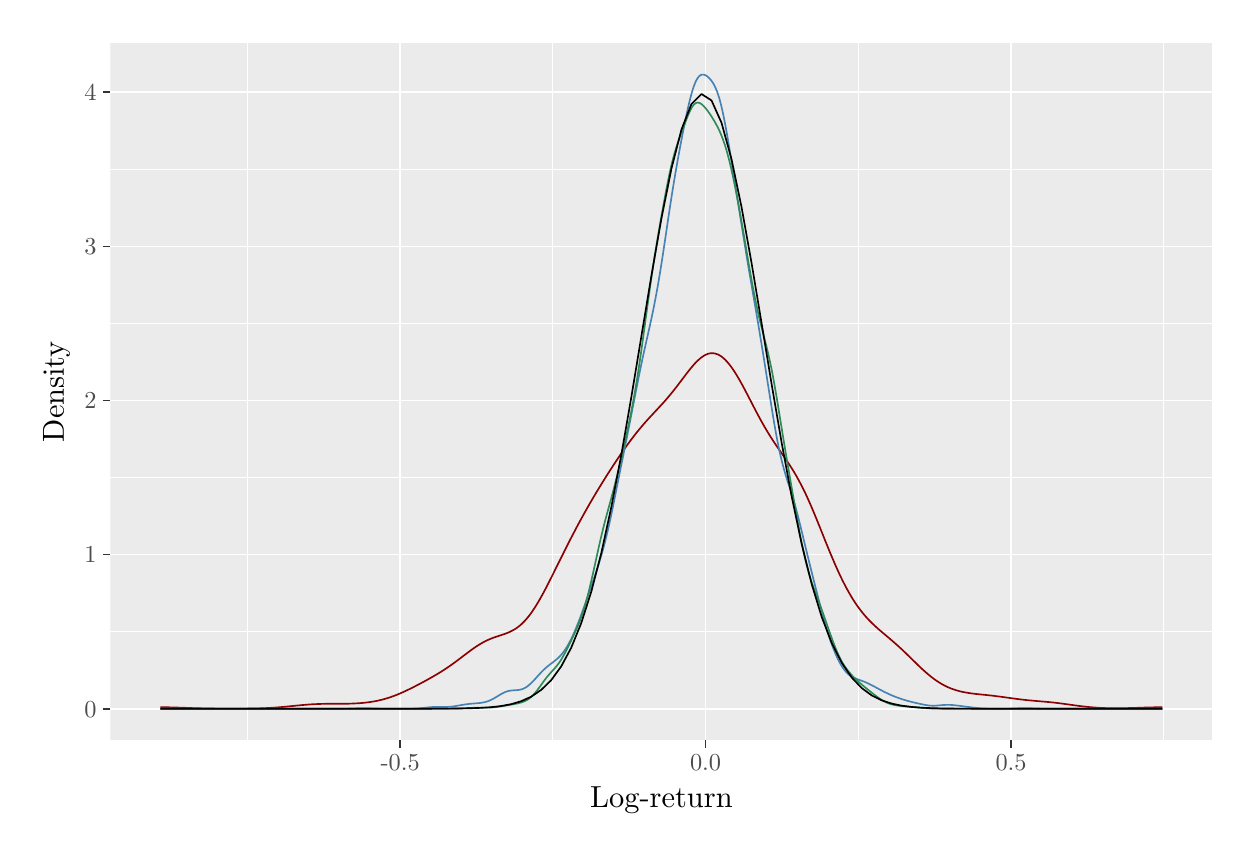
\begin{tikzpicture}[x=1pt,y=1pt]
\definecolor{fillColor}{RGB}{255,255,255}
\path[use as bounding box,fill=fillColor,fill opacity=0.00] (0,0) rectangle (433.62,289.08);
\begin{scope}
\path[clip] (  0.00,  0.00) rectangle (433.62,289.08);
\definecolor{drawColor}{RGB}{255,255,255}
\definecolor{fillColor}{RGB}{255,255,255}

\path[draw=drawColor,line width= 0.6pt,line join=round,line cap=round,fill=fillColor] (  0.00,  0.00) rectangle (433.62,289.08);
\end{scope}
\begin{scope}
\path[clip] ( 29.87, 31.53) rectangle (428.12,283.58);
\definecolor{fillColor}{gray}{0.92}

\path[fill=fillColor] ( 29.87, 31.53) rectangle (428.12,283.58);
\definecolor{drawColor}{RGB}{255,255,255}

\path[draw=drawColor,line width= 0.3pt,line join=round] ( 29.87, 70.83) --
	(428.12, 70.83);

\path[draw=drawColor,line width= 0.3pt,line join=round] ( 29.87,126.52) --
	(428.12,126.52);

\path[draw=drawColor,line width= 0.3pt,line join=round] ( 29.87,182.21) --
	(428.12,182.21);

\path[draw=drawColor,line width= 0.3pt,line join=round] ( 29.87,237.89) --
	(428.12,237.89);

\path[draw=drawColor,line width= 0.3pt,line join=round] ( 79.41, 31.53) --
	( 79.41,283.58);

\path[draw=drawColor,line width= 0.3pt,line join=round] (189.78, 31.53) --
	(189.78,283.58);

\path[draw=drawColor,line width= 0.3pt,line join=round] (300.16, 31.53) --
	(300.16,283.58);

\path[draw=drawColor,line width= 0.3pt,line join=round] (410.53, 31.53) --
	(410.53,283.58);

\path[draw=drawColor,line width= 0.6pt,line join=round] ( 29.87, 42.99) --
	(428.12, 42.99);

\path[draw=drawColor,line width= 0.6pt,line join=round] ( 29.87, 98.67) --
	(428.12, 98.67);

\path[draw=drawColor,line width= 0.6pt,line join=round] ( 29.87,154.36) --
	(428.12,154.36);

\path[draw=drawColor,line width= 0.6pt,line join=round] ( 29.87,210.05) --
	(428.12,210.05);

\path[draw=drawColor,line width= 0.6pt,line join=round] ( 29.87,265.74) --
	(428.12,265.74);

\path[draw=drawColor,line width= 0.6pt,line join=round] (134.60, 31.53) --
	(134.60,283.58);

\path[draw=drawColor,line width= 0.6pt,line join=round] (244.97, 31.53) --
	(244.97,283.58);

\path[draw=drawColor,line width= 0.6pt,line join=round] (355.35, 31.53) --
	(355.35,283.58);
\definecolor{drawColor}{RGB}{139,0,0}

\path[draw=drawColor,line width= 0.6pt,line join=round] ( 47.97, 43.52) --
	( 48.68, 43.52) --
	( 49.39, 43.51) --
	( 50.10, 43.50) --
	( 50.81, 43.49) --
	( 51.51, 43.48) --
	( 52.22, 43.46) --
	( 52.93, 43.44) --
	( 53.64, 43.42) --
	( 54.35, 43.40) --
	( 55.06, 43.37) --
	( 55.76, 43.35) --
	( 56.47, 43.32) --
	( 57.18, 43.30) --
	( 57.89, 43.27) --
	( 58.60, 43.25) --
	( 59.31, 43.22) --
	( 60.02, 43.20) --
	( 60.72, 43.18) --
	( 61.43, 43.16) --
	( 62.14, 43.14) --
	( 62.85, 43.12) --
	( 63.56, 43.10) --
	( 64.27, 43.09) --
	( 64.98, 43.07) --
	( 65.68, 43.06) --
	( 66.39, 43.05) --
	( 67.10, 43.04) --
	( 67.81, 43.03) --
	( 68.52, 43.02) --
	( 69.23, 43.02) --
	( 69.93, 43.01) --
	( 70.64, 43.01) --
	( 71.35, 43.01) --
	( 72.06, 43.00) --
	( 72.77, 43.00) --
	( 73.48, 43.00) --
	( 74.19, 43.00) --
	( 74.89, 43.00) --
	( 75.60, 43.00) --
	( 76.31, 43.01) --
	( 77.02, 43.01) --
	( 77.73, 43.01) --
	( 78.44, 43.02) --
	( 79.15, 43.03) --
	( 79.85, 43.04) --
	( 80.56, 43.05) --
	( 81.27, 43.06) --
	( 81.98, 43.07) --
	( 82.69, 43.09) --
	( 83.40, 43.11) --
	( 84.10, 43.13) --
	( 84.81, 43.15) --
	( 85.52, 43.18) --
	( 86.23, 43.21) --
	( 86.94, 43.25) --
	( 87.65, 43.29) --
	( 88.36, 43.33) --
	( 89.06, 43.37) --
	( 89.77, 43.42) --
	( 90.48, 43.48) --
	( 91.19, 43.54) --
	( 91.90, 43.60) --
	( 92.61, 43.66) --
	( 93.32, 43.73) --
	( 94.02, 43.80) --
	( 94.73, 43.87) --
	( 95.44, 43.94) --
	( 96.15, 44.01) --
	( 96.86, 44.08) --
	( 97.57, 44.15) --
	( 98.28, 44.22) --
	( 98.98, 44.29) --
	( 99.69, 44.35) --
	(100.40, 44.41) --
	(101.11, 44.47) --
	(101.82, 44.52) --
	(102.53, 44.57) --
	(103.23, 44.61) --
	(103.94, 44.64) --
	(104.65, 44.67) --
	(105.36, 44.70) --
	(106.07, 44.72) --
	(106.78, 44.74) --
	(107.49, 44.75) --
	(108.19, 44.75) --
	(108.90, 44.76) --
	(109.61, 44.76) --
	(110.32, 44.76) --
	(111.03, 44.76) --
	(111.74, 44.76) --
	(112.45, 44.76) --
	(113.15, 44.76) --
	(113.86, 44.77) --
	(114.57, 44.78) --
	(115.28, 44.79) --
	(115.99, 44.80) --
	(116.70, 44.82) --
	(117.40, 44.85) --
	(118.11, 44.88) --
	(118.82, 44.92) --
	(119.53, 44.96) --
	(120.24, 45.01) --
	(120.95, 45.07) --
	(121.66, 45.14) --
	(122.36, 45.22) --
	(123.07, 45.31) --
	(123.78, 45.41) --
	(124.49, 45.52) --
	(125.20, 45.64) --
	(125.91, 45.77) --
	(126.62, 45.92) --
	(127.32, 46.08) --
	(128.03, 46.25) --
	(128.74, 46.44) --
	(129.45, 46.64) --
	(130.16, 46.86) --
	(130.87, 47.09) --
	(131.57, 47.33) --
	(132.28, 47.59) --
	(132.99, 47.86) --
	(133.70, 48.14) --
	(134.41, 48.44) --
	(135.12, 48.75) --
	(135.83, 49.07) --
	(136.53, 49.39) --
	(137.24, 49.73) --
	(137.95, 50.07) --
	(138.66, 50.42) --
	(139.37, 50.78) --
	(140.08, 51.14) --
	(140.79, 51.51) --
	(141.49, 51.88) --
	(142.20, 52.25) --
	(142.91, 52.63) --
	(143.62, 53.02) --
	(144.33, 53.40) --
	(145.04, 53.80) --
	(145.74, 54.19) --
	(146.45, 54.60) --
	(147.16, 55.01) --
	(147.87, 55.43) --
	(148.58, 55.85) --
	(149.29, 56.29) --
	(150.00, 56.74) --
	(150.70, 57.20) --
	(151.41, 57.67) --
	(152.12, 58.15) --
	(152.83, 58.64) --
	(153.54, 59.14) --
	(154.25, 59.66) --
	(154.96, 60.18) --
	(155.66, 60.71) --
	(156.37, 61.25) --
	(157.08, 61.79) --
	(157.79, 62.33) --
	(158.50, 62.86) --
	(159.21, 63.40) --
	(159.92, 63.92) --
	(160.62, 64.44) --
	(161.33, 64.94) --
	(162.04, 65.42) --
	(162.75, 65.88) --
	(163.46, 66.32) --
	(164.17, 66.74) --
	(164.87, 67.12) --
	(165.58, 67.48) --
	(166.29, 67.82) --
	(167.00, 68.13) --
	(167.71, 68.42) --
	(168.42, 68.69) --
	(169.13, 68.93) --
	(169.83, 69.17) --
	(170.54, 69.40) --
	(171.25, 69.64) --
	(171.96, 69.87) --
	(172.67, 70.12) --
	(173.38, 70.39) --
	(174.09, 70.70) --
	(174.79, 71.03) --
	(175.50, 71.41) --
	(176.21, 71.83) --
	(176.92, 72.31) --
	(177.63, 72.85) --
	(178.34, 73.46) --
	(179.04, 74.13) --
	(179.75, 74.87) --
	(180.46, 75.68) --
	(181.17, 76.55) --
	(181.88, 77.50) --
	(182.59, 78.52) --
	(183.30, 79.60) --
	(184.00, 80.73) --
	(184.71, 81.92) --
	(185.42, 83.15) --
	(186.13, 84.44) --
	(186.84, 85.76) --
	(187.55, 87.12) --
	(188.26, 88.50) --
	(188.96, 89.90) --
	(189.67, 91.31) --
	(190.38, 92.74) --
	(191.09, 94.18) --
	(191.80, 95.61) --
	(192.51, 97.04) --
	(193.21, 98.47) --
	(193.92, 99.89) --
	(194.63,101.31) --
	(195.34,102.70) --
	(196.05,104.09) --
	(196.76,105.47) --
	(197.47,106.82) --
	(198.17,108.17) --
	(198.88,109.50) --
	(199.59,110.81) --
	(200.30,112.10) --
	(201.01,113.39) --
	(201.72,114.65) --
	(202.43,115.90) --
	(203.13,117.14) --
	(203.84,118.36) --
	(204.55,119.56) --
	(205.26,120.76) --
	(205.97,121.94) --
	(206.68,123.10) --
	(207.39,124.26) --
	(208.09,125.40) --
	(208.80,126.53) --
	(209.51,127.65) --
	(210.22,128.76) --
	(210.93,129.86) --
	(211.64,130.95) --
	(212.34,132.02) --
	(213.05,133.09) --
	(213.76,134.14) --
	(214.47,135.18) --
	(215.18,136.20) --
	(215.89,137.21) --
	(216.60,138.20) --
	(217.30,139.18) --
	(218.01,140.13) --
	(218.72,141.07) --
	(219.43,141.99) --
	(220.14,142.88) --
	(220.85,143.76) --
	(221.56,144.61) --
	(222.26,145.44) --
	(222.97,146.26) --
	(223.68,147.05) --
	(224.39,147.84) --
	(225.10,148.61) --
	(225.81,149.37) --
	(226.51,150.13) --
	(227.22,150.88) --
	(227.93,151.64) --
	(228.64,152.41) --
	(229.35,153.18) --
	(230.06,153.97) --
	(230.77,154.78) --
	(231.47,155.60) --
	(232.18,156.45) --
	(232.89,157.31) --
	(233.60,158.20) --
	(234.31,159.10) --
	(235.02,160.02) --
	(235.73,160.96) --
	(236.43,161.89) --
	(237.14,162.83) --
	(237.85,163.77) --
	(238.56,164.69) --
	(239.27,165.58) --
	(239.98,166.44) --
	(240.68,167.27) --
	(241.39,168.05) --
	(242.10,168.76) --
	(242.81,169.40) --
	(243.52,169.97) --
	(244.23,170.45) --
	(244.94,170.85) --
	(245.64,171.16) --
	(246.35,171.37) --
	(247.06,171.45) --
	(247.77,171.43) --
	(248.48,171.31) --
	(249.19,171.08) --
	(249.90,170.75) --
	(250.60,170.32) --
	(251.31,169.76) --
	(252.02,169.11) --
	(252.73,168.36) --
	(253.44,167.52) --
	(254.15,166.61) --
	(254.85,165.61) --
	(255.56,164.53) --
	(256.27,163.39) --
	(256.98,162.19) --
	(257.69,160.94) --
	(258.40,159.65) --
	(259.11,158.33) --
	(259.81,156.98) --
	(260.52,155.61) --
	(261.23,154.24) --
	(261.94,152.87) --
	(262.65,151.50) --
	(263.36,150.14) --
	(264.07,148.81) --
	(264.77,147.50) --
	(265.48,146.23) --
	(266.19,144.98) --
	(266.90,143.77) --
	(267.61,142.59) --
	(268.32,141.45) --
	(269.03,140.34) --
	(269.73,139.26) --
	(270.44,138.20) --
	(271.15,137.16) --
	(271.86,136.14) --
	(272.57,135.12) --
	(273.28,134.10) --
	(273.98,133.07) --
	(274.69,132.02) --
	(275.40,130.94) --
	(276.11,129.84) --
	(276.82,128.69) --
	(277.53,127.49) --
	(278.24,126.24) --
	(278.94,124.94) --
	(279.65,123.58) --
	(280.36,122.17) --
	(281.07,120.70) --
	(281.78,119.17) --
	(282.49,117.58) --
	(283.20,115.96) --
	(283.90,114.29) --
	(284.61,112.59) --
	(285.32,110.85) --
	(286.03,109.10) --
	(286.74,107.33) --
	(287.45,105.56) --
	(288.15,103.79) --
	(288.86,102.04) --
	(289.57,100.30) --
	(290.28, 98.59) --
	(290.99, 96.91) --
	(291.70, 95.27) --
	(292.41, 93.66) --
	(293.11, 92.11) --
	(293.82, 90.60) --
	(294.53, 89.15) --
	(295.24, 87.76) --
	(295.95, 86.42) --
	(296.66, 85.14) --
	(297.37, 83.91) --
	(298.07, 82.74) --
	(298.78, 81.63) --
	(299.49, 80.58) --
	(300.20, 79.58) --
	(300.91, 78.63) --
	(301.62, 77.72) --
	(302.32, 76.87) --
	(303.03, 76.06) --
	(303.74, 75.29) --
	(304.45, 74.55) --
	(305.16, 73.85) --
	(305.87, 73.17) --
	(306.58, 72.52) --
	(307.28, 71.88) --
	(307.99, 71.27) --
	(308.70, 70.66) --
	(309.41, 70.06) --
	(310.12, 69.47) --
	(310.83, 68.87) --
	(311.54, 68.27) --
	(312.24, 67.67) --
	(312.95, 67.05) --
	(313.66, 66.43) --
	(314.37, 65.80) --
	(315.08, 65.15) --
	(315.79, 64.50) --
	(316.49, 63.83) --
	(317.20, 63.15) --
	(317.91, 62.46) --
	(318.62, 61.77) --
	(319.33, 61.08) --
	(320.04, 60.38) --
	(320.75, 59.69) --
	(321.45, 59.00) --
	(322.16, 58.32) --
	(322.87, 57.65) --
	(323.58, 57.00) --
	(324.29, 56.36) --
	(325.00, 55.74) --
	(325.71, 55.15) --
	(326.41, 54.57) --
	(327.12, 54.02) --
	(327.83, 53.50) --
	(328.54, 53.01) --
	(329.25, 52.54) --
	(329.96, 52.11) --
	(330.67, 51.70) --
	(331.37, 51.33) --
	(332.08, 50.98) --
	(332.79, 50.65) --
	(333.50, 50.36) --
	(334.21, 50.09) --
	(334.92, 49.85) --
	(335.62, 49.63) --
	(336.33, 49.42) --
	(337.04, 49.24) --
	(337.75, 49.08) --
	(338.46, 48.94) --
	(339.17, 48.81) --
	(339.88, 48.69) --
	(340.58, 48.58) --
	(341.29, 48.48) --
	(342.00, 48.40) --
	(342.71, 48.31) --
	(343.42, 48.24) --
	(344.13, 48.16) --
	(344.84, 48.09) --
	(345.54, 48.02) --
	(346.25, 47.95) --
	(346.96, 47.87) --
	(347.67, 47.80) --
	(348.38, 47.72) --
	(349.09, 47.64) --
	(349.79, 47.55) --
	(350.50, 47.46) --
	(351.21, 47.37) --
	(351.92, 47.28) --
	(352.63, 47.18) --
	(353.34, 47.08) --
	(354.05, 46.98) --
	(354.75, 46.88) --
	(355.46, 46.78) --
	(356.17, 46.69) --
	(356.88, 46.59) --
	(357.59, 46.50) --
	(358.30, 46.41) --
	(359.01, 46.32) --
	(359.71, 46.24) --
	(360.42, 46.16) --
	(361.13, 46.09) --
	(361.84, 46.02) --
	(362.55, 45.95) --
	(363.26, 45.89) --
	(363.96, 45.82) --
	(364.67, 45.76) --
	(365.38, 45.70) --
	(366.09, 45.64) --
	(366.80, 45.58) --
	(367.51, 45.52) --
	(368.22, 45.46) --
	(368.92, 45.39) --
	(369.63, 45.32) --
	(370.34, 45.25) --
	(371.05, 45.17) --
	(371.76, 45.09) --
	(372.47, 45.00) --
	(373.18, 44.91) --
	(373.88, 44.82) --
	(374.59, 44.72) --
	(375.30, 44.63) --
	(376.01, 44.53) --
	(376.72, 44.43) --
	(377.43, 44.33) --
	(378.13, 44.23) --
	(378.84, 44.14) --
	(379.55, 44.04) --
	(380.26, 43.95) --
	(380.97, 43.86) --
	(381.68, 43.78) --
	(382.39, 43.70) --
	(383.09, 43.63) --
	(383.80, 43.56) --
	(384.51, 43.50) --
	(385.22, 43.44) --
	(385.93, 43.39) --
	(386.64, 43.34) --
	(387.35, 43.30) --
	(388.05, 43.26) --
	(388.76, 43.23) --
	(389.47, 43.21) --
	(390.18, 43.19) --
	(390.89, 43.17) --
	(391.60, 43.16) --
	(392.31, 43.15) --
	(393.01, 43.15) --
	(393.72, 43.15) --
	(394.43, 43.15) --
	(395.14, 43.16) --
	(395.85, 43.17) --
	(396.56, 43.18) --
	(397.26, 43.20) --
	(397.97, 43.22) --
	(398.68, 43.24) --
	(399.39, 43.26) --
	(400.10, 43.28) --
	(400.81, 43.30) --
	(401.52, 43.33) --
	(402.22, 43.35) --
	(402.93, 43.38) --
	(403.64, 43.40) --
	(404.35, 43.42) --
	(405.06, 43.44) --
	(405.77, 43.46) --
	(406.48, 43.48) --
	(407.18, 43.49) --
	(407.89, 43.50) --
	(408.60, 43.51) --
	(409.31, 43.52) --
	(410.02, 43.52);
\definecolor{drawColor}{RGB}{70,130,180}

\path[draw=drawColor,line width= 0.6pt,line join=round] ( 47.97, 42.99) --
	( 48.68, 42.99) --
	( 49.39, 42.99) --
	( 50.10, 42.99) --
	( 50.81, 42.99) --
	( 51.51, 42.99) --
	( 52.22, 42.99) --
	( 52.93, 42.99) --
	( 53.64, 42.99) --
	( 54.35, 42.99) --
	( 55.06, 42.99) --
	( 55.76, 42.99) --
	( 56.47, 42.99) --
	( 57.18, 42.99) --
	( 57.89, 42.99) --
	( 58.60, 42.99) --
	( 59.31, 42.99) --
	( 60.02, 42.99) --
	( 60.72, 42.99) --
	( 61.43, 42.99) --
	( 62.14, 42.99) --
	( 62.85, 42.99) --
	( 63.56, 42.99) --
	( 64.27, 42.99) --
	( 64.98, 42.99) --
	( 65.68, 42.99) --
	( 66.39, 42.99) --
	( 67.10, 42.99) --
	( 67.81, 42.99) --
	( 68.52, 42.99) --
	( 69.23, 42.99) --
	( 69.93, 42.99) --
	( 70.64, 42.99) --
	( 71.35, 42.99) --
	( 72.06, 42.99) --
	( 72.77, 42.99) --
	( 73.48, 42.99) --
	( 74.19, 42.99) --
	( 74.89, 42.99) --
	( 75.60, 42.99) --
	( 76.31, 42.99) --
	( 77.02, 42.99) --
	( 77.73, 42.99) --
	( 78.44, 42.99) --
	( 79.15, 42.99) --
	( 79.85, 42.99) --
	( 80.56, 42.99) --
	( 81.27, 42.99) --
	( 81.98, 42.99) --
	( 82.69, 42.99) --
	( 83.40, 42.99) --
	( 84.10, 42.99) --
	( 84.81, 42.99) --
	( 85.52, 42.99) --
	( 86.23, 42.99) --
	( 86.94, 42.99) --
	( 87.65, 42.99) --
	( 88.36, 42.99) --
	( 89.06, 42.99) --
	( 89.77, 42.99) --
	( 90.48, 42.99) --
	( 91.19, 42.99) --
	( 91.90, 42.99) --
	( 92.61, 42.99) --
	( 93.32, 42.99) --
	( 94.02, 42.99) --
	( 94.73, 42.99) --
	( 95.44, 42.99) --
	( 96.15, 42.99) --
	( 96.86, 42.99) --
	( 97.57, 42.99) --
	( 98.28, 42.99) --
	( 98.98, 42.99) --
	( 99.69, 42.99) --
	(100.40, 42.99) --
	(101.11, 42.99) --
	(101.82, 42.99) --
	(102.53, 42.99) --
	(103.23, 42.99) --
	(103.94, 42.99) --
	(104.65, 42.99) --
	(105.36, 42.99) --
	(106.07, 42.99) --
	(106.78, 42.99) --
	(107.49, 42.99) --
	(108.19, 42.99) --
	(108.90, 42.99) --
	(109.61, 42.99) --
	(110.32, 42.99) --
	(111.03, 42.99) --
	(111.74, 42.99) --
	(112.45, 42.99) --
	(113.15, 43.00) --
	(113.86, 43.00) --
	(114.57, 43.01) --
	(115.28, 43.02) --
	(115.99, 43.04) --
	(116.70, 43.06) --
	(117.40, 43.08) --
	(118.11, 43.10) --
	(118.82, 43.13) --
	(119.53, 43.15) --
	(120.24, 43.17) --
	(120.95, 43.17) --
	(121.66, 43.18) --
	(122.36, 43.17) --
	(123.07, 43.15) --
	(123.78, 43.13) --
	(124.49, 43.11) --
	(125.20, 43.08) --
	(125.91, 43.06) --
	(126.62, 43.04) --
	(127.32, 43.02) --
	(128.03, 43.01) --
	(128.74, 43.00) --
	(129.45, 43.00) --
	(130.16, 42.99) --
	(130.87, 42.99) --
	(131.57, 42.99) --
	(132.28, 42.99) --
	(132.99, 42.99) --
	(133.70, 42.99) --
	(134.41, 42.99) --
	(135.12, 42.99) --
	(135.83, 42.99) --
	(136.53, 42.99) --
	(137.24, 43.00) --
	(137.95, 43.00) --
	(138.66, 43.01) --
	(139.37, 43.03) --
	(140.08, 43.06) --
	(140.79, 43.09) --
	(141.49, 43.14) --
	(142.20, 43.20) --
	(142.91, 43.27) --
	(143.62, 43.34) --
	(144.33, 43.42) --
	(145.04, 43.49) --
	(145.74, 43.55) --
	(146.45, 43.60) --
	(147.16, 43.62) --
	(147.87, 43.63) --
	(148.58, 43.62) --
	(149.29, 43.61) --
	(150.00, 43.60) --
	(150.70, 43.60) --
	(151.41, 43.61) --
	(152.12, 43.65) --
	(152.83, 43.70) --
	(153.54, 43.78) --
	(154.25, 43.88) --
	(154.96, 44.00) --
	(155.66, 44.12) --
	(156.37, 44.25) --
	(157.08, 44.37) --
	(157.79, 44.49) --
	(158.50, 44.59) --
	(159.21, 44.68) --
	(159.92, 44.76) --
	(160.62, 44.82) --
	(161.33, 44.88) --
	(162.04, 44.93) --
	(162.75, 44.99) --
	(163.46, 45.06) --
	(164.17, 45.16) --
	(164.87, 45.30) --
	(165.58, 45.47) --
	(166.29, 45.70) --
	(167.00, 45.98) --
	(167.71, 46.32) --
	(168.42, 46.69) --
	(169.13, 47.10) --
	(169.83, 47.53) --
	(170.54, 47.96) --
	(171.25, 48.37) --
	(171.96, 48.74) --
	(172.67, 49.05) --
	(173.38, 49.29) --
	(174.09, 49.46) --
	(174.79, 49.57) --
	(175.50, 49.63) --
	(176.21, 49.67) --
	(176.92, 49.71) --
	(177.63, 49.79) --
	(178.34, 49.95) --
	(179.04, 50.19) --
	(179.75, 50.53) --
	(180.46, 50.99) --
	(181.17, 51.54) --
	(181.88, 52.18) --
	(182.59, 52.89) --
	(183.30, 53.65) --
	(184.00, 54.43) --
	(184.71, 55.21) --
	(185.42, 55.98) --
	(186.13, 56.71) --
	(186.84, 57.39) --
	(187.55, 58.02) --
	(188.26, 58.60) --
	(188.96, 59.15) --
	(189.67, 59.68) --
	(190.38, 60.23) --
	(191.09, 60.80) --
	(191.80, 61.43) --
	(192.51, 62.15) --
	(193.21, 62.97) --
	(193.92, 63.90) --
	(194.63, 64.96) --
	(195.34, 66.16) --
	(196.05, 67.48) --
	(196.76, 68.91) --
	(197.47, 70.47) --
	(198.17, 72.13) --
	(198.88, 73.89) --
	(199.59, 75.74) --
	(200.30, 77.66) --
	(201.01, 79.63) --
	(201.72, 81.64) --
	(202.43, 83.68) --
	(203.13, 85.72) --
	(203.84, 87.77) --
	(204.55, 89.84) --
	(205.26, 91.94) --
	(205.97, 94.10) --
	(206.68, 96.35) --
	(207.39, 98.72) --
	(208.09,101.25) --
	(208.80,103.97) --
	(209.51,106.90) --
	(210.22,110.01) --
	(210.93,113.30) --
	(211.64,116.73) --
	(212.34,120.24) --
	(213.05,123.80) --
	(213.76,127.36) --
	(214.47,130.89) --
	(215.18,134.40) --
	(215.89,137.90) --
	(216.60,141.42) --
	(217.30,144.98) --
	(218.01,148.59) --
	(218.72,152.25) --
	(219.43,155.92) --
	(220.14,159.56) --
	(220.85,163.12) --
	(221.56,166.57) --
	(222.26,169.91) --
	(222.97,173.14) --
	(223.68,176.30) --
	(224.39,179.44) --
	(225.10,182.63) --
	(225.81,185.94) --
	(226.51,189.44) --
	(227.22,193.16) --
	(227.93,197.16) --
	(228.64,201.43) --
	(229.35,205.94) --
	(230.06,210.64) --
	(230.77,215.42) --
	(231.47,220.19) --
	(232.18,224.88) --
	(232.89,229.43) --
	(233.60,233.80) --
	(234.31,237.97) --
	(235.02,241.98) --
	(235.73,245.83) --
	(236.43,249.55) --
	(237.14,253.15) --
	(237.85,256.62) --
	(238.56,259.90) --
	(239.27,262.93) --
	(239.98,265.61) --
	(240.68,267.85) --
	(241.39,269.62) --
	(242.10,270.90) --
	(242.81,271.71) --
	(243.52,272.09) --
	(244.23,272.12) --
	(244.94,271.88) --
	(245.64,271.42) --
	(246.35,270.77) --
	(247.06,269.94) --
	(247.77,268.88) --
	(248.48,267.53) --
	(249.19,265.81) --
	(249.90,263.66) --
	(250.60,260.99) --
	(251.31,257.86) --
	(252.02,254.30) --
	(252.73,250.39) --
	(253.44,246.23) --
	(254.15,241.90) --
	(254.85,237.48) --
	(255.56,233.00) --
	(256.27,228.50) --
	(256.98,224.01) --
	(257.69,219.54) --
	(258.40,215.10) --
	(259.11,210.72) --
	(259.81,206.40) --
	(260.52,202.17) --
	(261.23,198.01) --
	(261.94,193.89) --
	(262.65,189.78) --
	(263.36,185.65) --
	(264.07,181.47) --
	(264.77,177.22) --
	(265.48,172.89) --
	(266.19,168.48) --
	(266.90,164.00) --
	(267.61,159.49) --
	(268.32,155.00) --
	(269.03,150.57) --
	(269.73,146.30) --
	(270.44,142.25) --
	(271.15,138.52) --
	(271.86,135.17) --
	(272.57,132.18) --
	(273.28,129.52) --
	(273.98,127.12) --
	(274.69,124.88) --
	(275.40,122.70) --
	(276.11,120.47) --
	(276.82,118.12) --
	(277.53,115.62) --
	(278.24,112.96) --
	(278.94,110.17) --
	(279.65,107.27) --
	(280.36,104.33) --
	(281.07,101.39) --
	(281.78, 98.47) --
	(282.49, 95.59) --
	(283.20, 92.75) --
	(283.90, 89.94) --
	(284.61, 87.14) --
	(285.32, 84.36) --
	(286.03, 81.62) --
	(286.74, 78.92) --
	(287.45, 76.30) --
	(288.15, 73.78) --
	(288.86, 71.38) --
	(289.57, 69.13) --
	(290.28, 67.03) --
	(290.99, 65.09) --
	(291.70, 63.31) --
	(292.41, 61.69) --
	(293.11, 60.23) --
	(293.82, 58.93) --
	(294.53, 57.79) --
	(295.24, 56.82) --
	(295.95, 56.01) --
	(296.66, 55.34) --
	(297.37, 54.81) --
	(298.07, 54.38) --
	(298.78, 54.04) --
	(299.49, 53.75) --
	(300.20, 53.50) --
	(300.91, 53.25) --
	(301.62, 52.99) --
	(302.32, 52.72) --
	(303.03, 52.42) --
	(303.74, 52.09) --
	(304.45, 51.75) --
	(305.16, 51.39) --
	(305.87, 51.02) --
	(306.58, 50.64) --
	(307.28, 50.26) --
	(307.99, 49.88) --
	(308.70, 49.51) --
	(309.41, 49.14) --
	(310.12, 48.79) --
	(310.83, 48.45) --
	(311.54, 48.12) --
	(312.24, 47.81) --
	(312.95, 47.52) --
	(313.66, 47.24) --
	(314.37, 46.98) --
	(315.08, 46.73) --
	(315.79, 46.49) --
	(316.49, 46.26) --
	(317.20, 46.05) --
	(317.91, 45.84) --
	(318.62, 45.64) --
	(319.33, 45.46) --
	(320.04, 45.29) --
	(320.75, 45.12) --
	(321.45, 44.96) --
	(322.16, 44.80) --
	(322.87, 44.65) --
	(323.58, 44.50) --
	(324.29, 44.36) --
	(325.00, 44.24) --
	(325.71, 44.15) --
	(326.41, 44.09) --
	(327.12, 44.07) --
	(327.83, 44.08) --
	(328.54, 44.12) --
	(329.25, 44.18) --
	(329.96, 44.25) --
	(330.67, 44.31) --
	(331.37, 44.35) --
	(332.08, 44.38) --
	(332.79, 44.38) --
	(333.50, 44.36) --
	(334.21, 44.31) --
	(334.92, 44.24) --
	(335.62, 44.16) --
	(336.33, 44.08) --
	(337.04, 43.99) --
	(337.75, 43.90) --
	(338.46, 43.80) --
	(339.17, 43.71) --
	(339.88, 43.62) --
	(340.58, 43.53) --
	(341.29, 43.44) --
	(342.00, 43.36) --
	(342.71, 43.28) --
	(343.42, 43.21) --
	(344.13, 43.15) --
	(344.84, 43.10) --
	(345.54, 43.07) --
	(346.25, 43.04) --
	(346.96, 43.02) --
	(347.67, 43.01) --
	(348.38, 43.00) --
	(349.09, 42.99) --
	(349.79, 42.99) --
	(350.50, 42.99) --
	(351.21, 42.99) --
	(351.92, 43.00) --
	(352.63, 43.00) --
	(353.34, 43.01) --
	(354.05, 43.02) --
	(354.75, 43.03) --
	(355.46, 43.05) --
	(356.17, 43.07) --
	(356.88, 43.10) --
	(357.59, 43.12) --
	(358.30, 43.14) --
	(359.01, 43.16) --
	(359.71, 43.17) --
	(360.42, 43.18) --
	(361.13, 43.17) --
	(361.84, 43.16) --
	(362.55, 43.14) --
	(363.26, 43.12) --
	(363.96, 43.09) --
	(364.67, 43.07) --
	(365.38, 43.05) --
	(366.09, 43.03) --
	(366.80, 43.02) --
	(367.51, 43.01) --
	(368.22, 43.00) --
	(368.92, 42.99) --
	(369.63, 42.99) --
	(370.34, 42.99) --
	(371.05, 42.99) --
	(371.76, 42.99) --
	(372.47, 42.99) --
	(373.18, 42.99) --
	(373.88, 42.99) --
	(374.59, 42.99) --
	(375.30, 42.99) --
	(376.01, 42.99) --
	(376.72, 42.99) --
	(377.43, 42.99) --
	(378.13, 42.99) --
	(378.84, 42.99) --
	(379.55, 42.99) --
	(380.26, 42.99) --
	(380.97, 42.99) --
	(381.68, 42.99) --
	(382.39, 42.99) --
	(383.09, 42.99) --
	(383.80, 42.99) --
	(384.51, 42.99) --
	(385.22, 42.99) --
	(385.93, 42.99) --
	(386.64, 42.99) --
	(387.35, 42.99) --
	(388.05, 42.99) --
	(388.76, 42.99) --
	(389.47, 42.99) --
	(390.18, 42.99) --
	(390.89, 42.99) --
	(391.60, 42.99) --
	(392.31, 42.99) --
	(393.01, 42.99) --
	(393.72, 42.99) --
	(394.43, 42.99) --
	(395.14, 42.99) --
	(395.85, 42.99) --
	(396.56, 42.99) --
	(397.26, 42.99) --
	(397.97, 42.99) --
	(398.68, 42.99) --
	(399.39, 42.99) --
	(400.10, 42.99) --
	(400.81, 42.99) --
	(401.52, 42.99) --
	(402.22, 42.99) --
	(402.93, 42.99) --
	(403.64, 42.99) --
	(404.35, 42.99) --
	(405.06, 42.99) --
	(405.77, 42.99) --
	(406.48, 42.99) --
	(407.18, 42.99) --
	(407.89, 42.99) --
	(408.60, 42.99) --
	(409.31, 42.99) --
	(410.02, 42.99);
\definecolor{drawColor}{RGB}{46,139,87}

\path[draw=drawColor,line width= 0.6pt,line join=round] ( 47.97, 42.99) --
	( 48.68, 42.99) --
	( 49.39, 42.99) --
	( 50.10, 42.99) --
	( 50.81, 42.99) --
	( 51.51, 42.99) --
	( 52.22, 42.99) --
	( 52.93, 42.99) --
	( 53.64, 42.99) --
	( 54.35, 42.99) --
	( 55.06, 42.99) --
	( 55.76, 42.99) --
	( 56.47, 42.99) --
	( 57.18, 42.99) --
	( 57.89, 42.99) --
	( 58.60, 42.99) --
	( 59.31, 42.99) --
	( 60.02, 42.99) --
	( 60.72, 42.99) --
	( 61.43, 42.99) --
	( 62.14, 42.99) --
	( 62.85, 42.99) --
	( 63.56, 42.99) --
	( 64.27, 42.99) --
	( 64.98, 42.99) --
	( 65.68, 42.99) --
	( 66.39, 42.99) --
	( 67.10, 42.99) --
	( 67.81, 42.99) --
	( 68.52, 42.99) --
	( 69.23, 42.99) --
	( 69.93, 42.99) --
	( 70.64, 42.99) --
	( 71.35, 42.99) --
	( 72.06, 42.99) --
	( 72.77, 42.99) --
	( 73.48, 42.99) --
	( 74.19, 42.99) --
	( 74.89, 42.99) --
	( 75.60, 42.99) --
	( 76.31, 42.99) --
	( 77.02, 42.99) --
	( 77.73, 42.99) --
	( 78.44, 42.99) --
	( 79.15, 42.99) --
	( 79.85, 42.99) --
	( 80.56, 42.99) --
	( 81.27, 42.99) --
	( 81.98, 42.99) --
	( 82.69, 42.99) --
	( 83.40, 42.99) --
	( 84.10, 42.99) --
	( 84.81, 42.99) --
	( 85.52, 42.99) --
	( 86.23, 42.99) --
	( 86.94, 42.99) --
	( 87.65, 42.99) --
	( 88.36, 42.99) --
	( 89.06, 42.99) --
	( 89.77, 42.99) --
	( 90.48, 42.99) --
	( 91.19, 42.99) --
	( 91.90, 42.99) --
	( 92.61, 42.99) --
	( 93.32, 42.99) --
	( 94.02, 42.99) --
	( 94.73, 42.99) --
	( 95.44, 42.99) --
	( 96.15, 42.99) --
	( 96.86, 42.99) --
	( 97.57, 42.99) --
	( 98.28, 42.99) --
	( 98.98, 42.99) --
	( 99.69, 42.99) --
	(100.40, 42.99) --
	(101.11, 42.99) --
	(101.82, 42.99) --
	(102.53, 42.99) --
	(103.23, 42.99) --
	(103.94, 42.99) --
	(104.65, 42.99) --
	(105.36, 42.99) --
	(106.07, 42.99) --
	(106.78, 42.99) --
	(107.49, 42.99) --
	(108.19, 42.99) --
	(108.90, 42.99) --
	(109.61, 42.99) --
	(110.32, 42.99) --
	(111.03, 42.99) --
	(111.74, 42.99) --
	(112.45, 42.99) --
	(113.15, 42.99) --
	(113.86, 42.99) --
	(114.57, 42.99) --
	(115.28, 42.99) --
	(115.99, 42.99) --
	(116.70, 42.99) --
	(117.40, 42.99) --
	(118.11, 42.99) --
	(118.82, 42.99) --
	(119.53, 42.99) --
	(120.24, 42.99) --
	(120.95, 42.99) --
	(121.66, 42.99) --
	(122.36, 42.99) --
	(123.07, 42.99) --
	(123.78, 42.99) --
	(124.49, 42.99) --
	(125.20, 42.99) --
	(125.91, 42.99) --
	(126.62, 42.99) --
	(127.32, 42.99) --
	(128.03, 42.99) --
	(128.74, 42.99) --
	(129.45, 42.99) --
	(130.16, 42.99) --
	(130.87, 42.99) --
	(131.57, 42.99) --
	(132.28, 42.99) --
	(132.99, 42.99) --
	(133.70, 42.99) --
	(134.41, 42.99) --
	(135.12, 42.99) --
	(135.83, 42.99) --
	(136.53, 42.99) --
	(137.24, 42.99) --
	(137.95, 42.99) --
	(138.66, 42.99) --
	(139.37, 42.99) --
	(140.08, 42.99) --
	(140.79, 42.99) --
	(141.49, 42.99) --
	(142.20, 42.99) --
	(142.91, 42.99) --
	(143.62, 42.99) --
	(144.33, 42.99) --
	(145.04, 42.99) --
	(145.74, 42.99) --
	(146.45, 42.99) --
	(147.16, 42.99) --
	(147.87, 42.99) --
	(148.58, 42.99) --
	(149.29, 42.99) --
	(150.00, 42.99) --
	(150.70, 42.99) --
	(151.41, 43.00) --
	(152.12, 43.00) --
	(152.83, 43.01) --
	(153.54, 43.03) --
	(154.25, 43.04) --
	(154.96, 43.06) --
	(155.66, 43.09) --
	(156.37, 43.12) --
	(157.08, 43.15) --
	(157.79, 43.18) --
	(158.50, 43.21) --
	(159.21, 43.24) --
	(159.92, 43.27) --
	(160.62, 43.30) --
	(161.33, 43.32) --
	(162.04, 43.34) --
	(162.75, 43.36) --
	(163.46, 43.37) --
	(164.17, 43.37) --
	(164.87, 43.37) --
	(165.58, 43.37) --
	(166.29, 43.38) --
	(167.00, 43.40) --
	(167.71, 43.43) --
	(168.42, 43.49) --
	(169.13, 43.56) --
	(169.83, 43.65) --
	(170.54, 43.76) --
	(171.25, 43.87) --
	(171.96, 43.99) --
	(172.67, 44.12) --
	(173.38, 44.24) --
	(174.09, 44.37) --
	(174.79, 44.49) --
	(175.50, 44.61) --
	(176.21, 44.74) --
	(176.92, 44.88) --
	(177.63, 45.04) --
	(178.34, 45.24) --
	(179.04, 45.48) --
	(179.75, 45.77) --
	(180.46, 46.15) --
	(181.17, 46.61) --
	(181.88, 47.17) --
	(182.59, 47.85) --
	(183.30, 48.62) --
	(184.00, 49.49) --
	(184.71, 50.44) --
	(185.42, 51.42) --
	(186.13, 52.42) --
	(186.84, 53.39) --
	(187.55, 54.31) --
	(188.26, 55.16) --
	(188.96, 55.96) --
	(189.67, 56.74) --
	(190.38, 57.52) --
	(191.09, 58.35) --
	(191.80, 59.26) --
	(192.51, 60.29) --
	(193.21, 61.43) --
	(193.92, 62.69) --
	(194.63, 64.03) --
	(195.34, 65.45) --
	(196.05, 66.90) --
	(196.76, 68.38) --
	(197.47, 69.89) --
	(198.17, 71.45) --
	(198.88, 73.10) --
	(199.59, 74.88) --
	(200.30, 76.84) --
	(201.01, 79.01) --
	(201.72, 81.42) --
	(202.43, 84.06) --
	(203.13, 86.92) --
	(203.84, 89.96) --
	(204.55, 93.13) --
	(205.26, 96.36) --
	(205.97, 99.60) --
	(206.68,102.76) --
	(207.39,105.81) --
	(208.09,108.69) --
	(208.80,111.44) --
	(209.51,114.07) --
	(210.22,116.65) --
	(210.93,119.23) --
	(211.64,121.86) --
	(212.34,124.58) --
	(213.05,127.42) --
	(213.76,130.36) --
	(214.47,133.40) --
	(215.18,136.52) --
	(215.89,139.71) --
	(216.60,142.98) --
	(217.30,146.35) --
	(218.01,149.86) --
	(218.72,153.57) --
	(219.43,157.53) --
	(220.14,161.77) --
	(220.85,166.31) --
	(221.56,171.12) --
	(222.26,176.15) --
	(222.97,181.33) --
	(223.68,186.56) --
	(224.39,191.73) --
	(225.10,196.75) --
	(225.81,201.57) --
	(226.51,206.17) --
	(227.22,210.56) --
	(227.93,214.78) --
	(228.64,218.87) --
	(229.35,222.87) --
	(230.06,226.77) --
	(230.77,230.55) --
	(231.47,234.14) --
	(232.18,237.48) --
	(232.89,240.50) --
	(233.60,243.20) --
	(234.31,245.60) --
	(235.02,247.75) --
	(235.73,249.75) --
	(236.43,251.67) --
	(237.14,253.56) --
	(237.85,255.44) --
	(238.56,257.25) --
	(239.27,258.89) --
	(239.98,260.26) --
	(240.68,261.25) --
	(241.39,261.83) --
	(242.10,262.02) --
	(242.81,261.87) --
	(243.52,261.43) --
	(244.23,260.79) --
	(244.94,260.00) --
	(245.64,259.10) --
	(246.35,258.12) --
	(247.06,257.06) --
	(247.77,255.93) --
	(248.48,254.71) --
	(249.19,253.40) --
	(249.90,251.96) --
	(250.60,250.35) --
	(251.31,248.52) --
	(252.02,246.42) --
	(252.73,244.05) --
	(253.44,241.39) --
	(254.15,238.45) --
	(254.85,235.27) --
	(255.56,231.86) --
	(256.27,228.24) --
	(256.98,224.45) --
	(257.69,220.50) --
	(258.40,216.43) --
	(259.11,212.26) --
	(259.81,208.06) --
	(260.52,203.88) --
	(261.23,199.79) --
	(261.94,195.86) --
	(262.65,192.15) --
	(263.36,188.69) --
	(264.07,185.47) --
	(264.77,182.48) --
	(265.48,179.65) --
	(266.19,176.89) --
	(266.90,174.10) --
	(267.61,171.17) --
	(268.32,168.00) --
	(269.03,164.52) --
	(269.73,160.73) --
	(270.44,156.66) --
	(271.15,152.39) --
	(271.86,148.01) --
	(272.57,143.61) --
	(273.28,139.28) --
	(273.98,135.03) --
	(274.69,130.85) --
	(275.40,126.73) --
	(276.11,122.63) --
	(276.82,118.55) --
	(277.53,114.49) --
	(278.24,110.51) --
	(278.94,106.66) --
	(279.65,103.01) --
	(280.36, 99.62) --
	(281.07, 96.52) --
	(281.78, 93.73) --
	(282.49, 91.23) --
	(283.20, 88.98) --
	(283.90, 86.92) --
	(284.61, 84.97) --
	(285.32, 83.08) --
	(286.03, 81.20) --
	(286.74, 79.29) --
	(287.45, 77.33) --
	(288.15, 75.33) --
	(288.86, 73.29) --
	(289.57, 71.25) --
	(290.28, 69.24) --
	(290.99, 67.29) --
	(291.70, 65.44) --
	(292.41, 63.72) --
	(293.11, 62.13) --
	(293.82, 60.71) --
	(294.53, 59.44) --
	(295.24, 58.31) --
	(295.95, 57.31) --
	(296.66, 56.40) --
	(297.37, 55.58) --
	(298.07, 54.81) --
	(298.78, 54.10) --
	(299.49, 53.41) --
	(300.20, 52.76) --
	(300.91, 52.13) --
	(301.62, 51.52) --
	(302.32, 50.93) --
	(303.03, 50.35) --
	(303.74, 49.78) --
	(304.45, 49.21) --
	(305.16, 48.66) --
	(305.87, 48.10) --
	(306.58, 47.57) --
	(307.28, 47.05) --
	(307.99, 46.56) --
	(308.70, 46.10) --
	(309.41, 45.70) --
	(310.12, 45.34) --
	(310.83, 45.03) --
	(311.54, 44.77) --
	(312.24, 44.56) --
	(312.95, 44.38) --
	(313.66, 44.24) --
	(314.37, 44.12) --
	(315.08, 44.03) --
	(315.79, 43.95) --
	(316.49, 43.88) --
	(317.20, 43.81) --
	(317.91, 43.75) --
	(318.62, 43.70) --
	(319.33, 43.64) --
	(320.04, 43.58) --
	(320.75, 43.52) --
	(321.45, 43.45) --
	(322.16, 43.39) --
	(322.87, 43.32) --
	(323.58, 43.26) --
	(324.29, 43.20) --
	(325.00, 43.15) --
	(325.71, 43.10) --
	(326.41, 43.07) --
	(327.12, 43.04) --
	(327.83, 43.02) --
	(328.54, 43.01) --
	(329.25, 43.00) --
	(329.96, 43.00) --
	(330.67, 42.99) --
	(331.37, 42.99) --
	(332.08, 42.99) --
	(332.79, 42.99) --
	(333.50, 42.99) --
	(334.21, 42.99) --
	(334.92, 42.99) --
	(335.62, 42.99) --
	(336.33, 42.99) --
	(337.04, 42.99) --
	(337.75, 42.99) --
	(338.46, 42.99) --
	(339.17, 42.99) --
	(339.88, 42.99) --
	(340.58, 42.99) --
	(341.29, 42.99) --
	(342.00, 42.99) --
	(342.71, 42.99) --
	(343.42, 42.99) --
	(344.13, 42.99) --
	(344.84, 42.99) --
	(345.54, 42.99) --
	(346.25, 42.99) --
	(346.96, 42.99) --
	(347.67, 42.99) --
	(348.38, 42.99) --
	(349.09, 42.99) --
	(349.79, 42.99) --
	(350.50, 42.99) --
	(351.21, 42.99) --
	(351.92, 42.99) --
	(352.63, 42.99) --
	(353.34, 42.99) --
	(354.05, 42.99) --
	(354.75, 42.99) --
	(355.46, 42.99) --
	(356.17, 42.99) --
	(356.88, 42.99) --
	(357.59, 42.99) --
	(358.30, 42.99) --
	(359.01, 42.99) --
	(359.71, 42.99) --
	(360.42, 42.99) --
	(361.13, 42.99) --
	(361.84, 42.99) --
	(362.55, 42.99) --
	(363.26, 42.99) --
	(363.96, 42.99) --
	(364.67, 42.99) --
	(365.38, 42.99) --
	(366.09, 42.99) --
	(366.80, 42.99) --
	(367.51, 42.99) --
	(368.22, 42.99) --
	(368.92, 42.99) --
	(369.63, 42.99) --
	(370.34, 42.99) --
	(371.05, 42.99) --
	(371.76, 42.99) --
	(372.47, 42.99) --
	(373.18, 42.99) --
	(373.88, 42.99) --
	(374.59, 42.99) --
	(375.30, 42.99) --
	(376.01, 42.99) --
	(376.72, 42.99) --
	(377.43, 42.99) --
	(378.13, 42.99) --
	(378.84, 42.99) --
	(379.55, 42.99) --
	(380.26, 42.99) --
	(380.97, 42.99) --
	(381.68, 42.99) --
	(382.39, 42.99) --
	(383.09, 42.99) --
	(383.80, 42.99) --
	(384.51, 42.99) --
	(385.22, 42.99) --
	(385.93, 42.99) --
	(386.64, 42.99) --
	(387.35, 42.99) --
	(388.05, 42.99) --
	(388.76, 42.99) --
	(389.47, 42.99) --
	(390.18, 42.99) --
	(390.89, 42.99) --
	(391.60, 42.99) --
	(392.31, 42.99) --
	(393.01, 42.99) --
	(393.72, 42.99) --
	(394.43, 42.99) --
	(395.14, 42.99) --
	(395.85, 42.99) --
	(396.56, 42.99) --
	(397.26, 42.99) --
	(397.97, 42.99) --
	(398.68, 42.99) --
	(399.39, 42.99) --
	(400.10, 42.99) --
	(400.81, 42.99) --
	(401.52, 42.99) --
	(402.22, 42.99) --
	(402.93, 42.99) --
	(403.64, 42.99) --
	(404.35, 42.99) --
	(405.06, 42.99) --
	(405.77, 42.99) --
	(406.48, 42.99) --
	(407.18, 42.99) --
	(407.89, 42.99) --
	(408.60, 42.99) --
	(409.31, 42.99) --
	(410.02, 42.99);
\definecolor{drawColor}{RGB}{0,0,0}

\path[draw=drawColor,line width= 0.6pt,line join=round] ( 47.97, 42.99) --
	( 51.59, 42.99) --
	( 55.21, 42.99) --
	( 58.83, 42.99) --
	( 62.45, 42.99) --
	( 66.07, 42.99) --
	( 69.69, 42.99) --
	( 73.31, 42.99) --
	( 76.93, 42.99) --
	( 80.56, 42.99) --
	( 84.18, 42.99) --
	( 87.80, 42.99) --
	( 91.42, 42.99) --
	( 95.04, 42.99) --
	( 98.66, 42.99) --
	(102.28, 42.99) --
	(105.90, 42.99) --
	(109.52, 42.99) --
	(113.14, 42.99) --
	(116.76, 42.99) --
	(120.38, 42.99) --
	(124.00, 42.99) --
	(127.62, 42.99) --
	(131.24, 42.99) --
	(134.86, 42.99) --
	(138.48, 42.99) --
	(142.10, 42.99) --
	(145.72, 43.00) --
	(149.34, 43.01) --
	(152.96, 43.03) --
	(156.59, 43.08) --
	(160.21, 43.16) --
	(163.83, 43.30) --
	(167.45, 43.54) --
	(171.07, 43.95) --
	(174.69, 44.62) --
	(178.31, 45.69) --
	(181.93, 47.32) --
	(185.55, 49.77) --
	(189.17, 53.30) --
	(192.79, 58.27) --
	(196.41, 65.02) --
	(200.03, 73.92) --
	(203.65, 85.25) --
	(207.27, 99.21) --
	(210.89,115.79) --
	(214.51,134.75) --
	(218.13,155.59) --
	(221.75,177.50) --
	(225.37,199.40) --
	(228.99,220.04) --
	(232.61,238.08) --
	(236.24,252.26) --
	(239.86,261.51) --
	(243.48,265.11) --
	(247.10,262.78) --
	(250.72,254.71) --
	(254.34,241.51) --
	(257.96,224.20) --
	(261.58,204.01) --
	(265.20,182.27) --
	(268.82,160.27) --
	(272.44,139.12) --
	(276.06,119.70) --
	(279.68,102.57) --
	(283.30, 88.04) --
	(286.92, 76.15) --
	(290.54, 66.75) --
	(294.16, 59.56) --
	(297.78, 54.24) --
	(301.40, 50.43) --
	(305.02, 47.77) --
	(308.64, 45.99) --
	(312.27, 44.82) --
	(315.89, 44.07) --
	(319.51, 43.61) --
	(323.13, 43.34) --
	(326.75, 43.18) --
	(330.37, 43.09) --
	(333.99, 43.04) --
	(337.61, 43.01) --
	(341.23, 43.00) --
	(344.85, 42.99) --
	(348.47, 42.99) --
	(352.09, 42.99) --
	(355.71, 42.99) --
	(359.33, 42.99) --
	(362.95, 42.99) --
	(366.57, 42.99) --
	(370.19, 42.99) --
	(373.81, 42.99) --
	(377.43, 42.99) --
	(381.05, 42.99) --
	(384.67, 42.99) --
	(388.29, 42.99) --
	(391.92, 42.99) --
	(395.54, 42.99) --
	(399.16, 42.99) --
	(402.78, 42.99) --
	(406.40, 42.99) --
	(410.02, 42.99);
\end{scope}
\begin{scope}
\path[clip] (  0.00,  0.00) rectangle (433.62,289.08);
\definecolor{drawColor}{gray}{0.30}

\node[text=drawColor,anchor=base east,inner sep=0pt, outer sep=0pt, scale=  0.88] at ( 24.92, 39.96) {0};

\node[text=drawColor,anchor=base east,inner sep=0pt, outer sep=0pt, scale=  0.88] at ( 24.92, 95.64) {1};

\node[text=drawColor,anchor=base east,inner sep=0pt, outer sep=0pt, scale=  0.88] at ( 24.92,151.33) {2};

\node[text=drawColor,anchor=base east,inner sep=0pt, outer sep=0pt, scale=  0.88] at ( 24.92,207.02) {3};

\node[text=drawColor,anchor=base east,inner sep=0pt, outer sep=0pt, scale=  0.88] at ( 24.92,262.71) {4};
\end{scope}
\begin{scope}
\path[clip] (  0.00,  0.00) rectangle (433.62,289.08);
\definecolor{drawColor}{gray}{0.20}

\path[draw=drawColor,line width= 0.6pt,line join=round] ( 27.12, 42.99) --
	( 29.87, 42.99);

\path[draw=drawColor,line width= 0.6pt,line join=round] ( 27.12, 98.67) --
	( 29.87, 98.67);

\path[draw=drawColor,line width= 0.6pt,line join=round] ( 27.12,154.36) --
	( 29.87,154.36);

\path[draw=drawColor,line width= 0.6pt,line join=round] ( 27.12,210.05) --
	( 29.87,210.05);

\path[draw=drawColor,line width= 0.6pt,line join=round] ( 27.12,265.74) --
	( 29.87,265.74);
\end{scope}
\begin{scope}
\path[clip] (  0.00,  0.00) rectangle (433.62,289.08);
\definecolor{drawColor}{gray}{0.20}

\path[draw=drawColor,line width= 0.6pt,line join=round] (134.60, 28.78) --
	(134.60, 31.53);

\path[draw=drawColor,line width= 0.6pt,line join=round] (244.97, 28.78) --
	(244.97, 31.53);

\path[draw=drawColor,line width= 0.6pt,line join=round] (355.35, 28.78) --
	(355.35, 31.53);
\end{scope}
\begin{scope}
\path[clip] (  0.00,  0.00) rectangle (433.62,289.08);
\definecolor{drawColor}{gray}{0.30}

\node[text=drawColor,anchor=base,inner sep=0pt, outer sep=0pt, scale=  0.88] at (134.60, 20.52) {-0.5};

\node[text=drawColor,anchor=base,inner sep=0pt, outer sep=0pt, scale=  0.88] at (244.97, 20.52) {0.0};

\node[text=drawColor,anchor=base,inner sep=0pt, outer sep=0pt, scale=  0.88] at (355.35, 20.52) {0.5};
\end{scope}
\begin{scope}
\path[clip] (  0.00,  0.00) rectangle (433.62,289.08);
\definecolor{drawColor}{RGB}{0,0,0}

\node[text=drawColor,anchor=base,inner sep=0pt, outer sep=0pt, scale=  1.10] at (228.99,  7.44) {Log-return};
\end{scope}
\begin{scope}
\path[clip] (  0.00,  0.00) rectangle (433.62,289.08);
\definecolor{drawColor}{RGB}{0,0,0}

\node[text=drawColor,rotate= 90.00,anchor=base,inner sep=0pt, outer sep=0pt, scale=  1.10] at ( 13.08,157.56) {Density};
\end{scope}
\end{tikzpicture}
 
\floatfoot{Simulation of Heston time series. Data have been output by the R function \textit{heston()} which is an implementation of equation \crefrange{eq:other:hsvvol}{eq:other:rho} (see appendix \ref{sub:r:time:heston}, for more information). The parameters passed to the function are:  $S(0) = 50$,  $V(0) = 0.2$,  $T = 5$ (years, along with a time step of 365 measures per year),  $\alpha = 0$,  $\kappa = 0.5$,  $\Theta = 0.2$,  $\sigma = 0.1$ and $\rho = -1$. 
} 
\caption{Heson Framework Using Negative Correllated Brownian Motions}
\label{p:other:uncorrelatedheston}
\end{figure}


\begin{figure}[ht]
\centering
\input{figures/correlatHeston.tex}
\caption{Heson Framework Using Positive Correllated Brownian Motion}
\floatfoot{Simulation of Heston time series. Data have been output by the R function \textit{heston()} which is an implementation of equation \crefrange{eq:other:hsvvol}{eq:other:rho} (see appendix \ref{sub:r:time:heston}, for more information). The parameters passed to the function are:  $S(0) = 50$,  $V(0) = 0.2$,  $T = 5$ (years, along with a time step of 365 measures per year),  $\alpha = 0$,  $\kappa = 0.5$,  $\Theta = 0.2$,  $\sigma = 0.1$ and $\rho = 1$.
}
\label{p:other:correlatedheston}
\end{figure}



The usage of the aforementioned Heston model lies in the fact that the correlation between the CIR and asset processes' Brownian motions would notably explain the spot return skewness whereas the kurtosis of the distribution may be affected by the volatility parameter $\sigma$ of the volatility stochastic process (\cref{eq:other:hsvvol}), (\citet{heston1993})
It may consequently be consistent with what happens in the equity market, namely a sharp decrease in equity price implies an increase in stock volatility (\citet{criso2015}).
% Nevertheless, even though Heston model gives a framework with stochastic volatility, over the long--run the spot return would be characterized by a normal distribution as limiting distribution, with $\theta$ as variance per unit of time. By consequence, Black--Scholes--Merton should work well for such long term option.




%%%%%%%%%%%%%%%%%%%%%%%%%%%%%%%%%%%%%%%%%%%%%%%%
% SUBSECTION: Impact on skewness density return
%%%%%%%%%%%%%%%%%%%%%%%%%%%%%%%%%%%%%%%%%%%%%%%%
\subsection{Impact on log--return density's skewness}
\label{sub:hestonskewness}

Through the Heston stochastic volatility model, the skewness of the distribution of continuously compounded spot return may be affected by the parameter $\rho$. 

When a positive correlation exists between both Brownian motions, an increase in the volatility implies a rise in the asset price whereas a decrease in the volatility tend to lower the asset price.
In other words, when the uncertainty is high and consequently the changes in the asset price are numerous, these latter tend to be positive. 
That is why the distribution of the spot return is offset to the left with a right fat tail when $\rho$ is positive.

The opposite relation is noticed with negative correlation, namely, lower prices relate to higher volatility generating a left fat tail in the log–return distribution (\citet{heston1993}).
These statements are observed in \cref{p:other:heston:skewness}.



\begin{figure}[ht]
\centering
% Created by tikzDevice version 0.11 on 2018-04-12 12:39:31
% !TEX encoding = UTF-8 Unicode
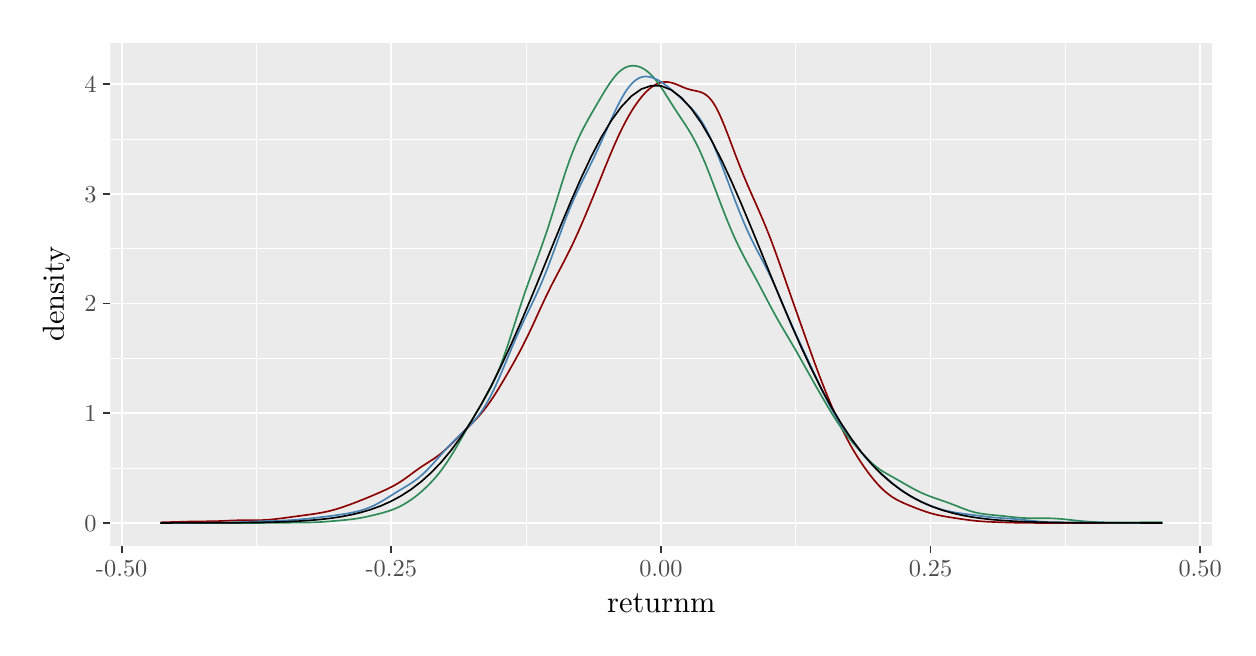
\begin{tikzpicture}[x=1pt,y=1pt]
\definecolor{fillColor}{RGB}{255,255,255}
\path[use as bounding box,fill=fillColor,fill opacity=0.00] (0,0) rectangle (433.62,216.81);
\begin{scope}
\path[clip] (  0.00,  0.00) rectangle (433.62,216.81);
\definecolor{drawColor}{RGB}{255,255,255}
\definecolor{fillColor}{RGB}{255,255,255}

\path[draw=drawColor,line width= 0.6pt,line join=round,line cap=round,fill=fillColor] (  0.00,  0.00) rectangle (433.62,216.81);
\end{scope}
\begin{scope}
\path[clip] ( 29.87, 29.59) rectangle (428.12,211.31);
\definecolor{fillColor}{gray}{0.92}

\path[fill=fillColor] ( 29.87, 29.59) rectangle (428.12,211.31);
\definecolor{drawColor}{RGB}{255,255,255}

\path[draw=drawColor,line width= 0.3pt,line join=round] ( 29.87, 57.67) --
	(428.12, 57.67);

\path[draw=drawColor,line width= 0.3pt,line join=round] ( 29.87, 97.30) --
	(428.12, 97.30);

\path[draw=drawColor,line width= 0.3pt,line join=round] ( 29.87,136.94) --
	(428.12,136.94);

\path[draw=drawColor,line width= 0.3pt,line join=round] ( 29.87,176.58) --
	(428.12,176.58);

\path[draw=drawColor,line width= 0.3pt,line join=round] ( 82.68, 29.59) --
	( 82.68,211.31);

\path[draw=drawColor,line width= 0.3pt,line join=round] (180.11, 29.59) --
	(180.11,211.31);

\path[draw=drawColor,line width= 0.3pt,line join=round] (277.54, 29.59) --
	(277.54,211.31);

\path[draw=drawColor,line width= 0.3pt,line join=round] (374.97, 29.59) --
	(374.97,211.31);

\path[draw=drawColor,line width= 0.6pt,line join=round] ( 29.87, 37.85) --
	(428.12, 37.85);

\path[draw=drawColor,line width= 0.6pt,line join=round] ( 29.87, 77.49) --
	(428.12, 77.49);

\path[draw=drawColor,line width= 0.6pt,line join=round] ( 29.87,117.12) --
	(428.12,117.12);

\path[draw=drawColor,line width= 0.6pt,line join=round] ( 29.87,156.76) --
	(428.12,156.76);

\path[draw=drawColor,line width= 0.6pt,line join=round] ( 29.87,196.40) --
	(428.12,196.40);

\path[draw=drawColor,line width= 0.6pt,line join=round] ( 33.97, 29.59) --
	( 33.97,211.31);

\path[draw=drawColor,line width= 0.6pt,line join=round] (131.40, 29.59) --
	(131.40,211.31);

\path[draw=drawColor,line width= 0.6pt,line join=round] (228.83, 29.59) --
	(228.83,211.31);

\path[draw=drawColor,line width= 0.6pt,line join=round] (326.26, 29.59) --
	(326.26,211.31);

\path[draw=drawColor,line width= 0.6pt,line join=round] (423.69, 29.59) --
	(423.69,211.31);
\definecolor{drawColor}{RGB}{139,0,0}

\path[draw=drawColor,line width= 0.6pt,line join=round] ( 47.97, 38.05) --
	( 48.68, 38.07) --
	( 49.39, 38.09) --
	( 50.10, 38.11) --
	( 50.81, 38.13) --
	( 51.51, 38.15) --
	( 52.22, 38.17) --
	( 52.93, 38.19) --
	( 53.64, 38.21) --
	( 54.35, 38.23) --
	( 55.06, 38.25) --
	( 55.76, 38.27) --
	( 56.47, 38.29) --
	( 57.18, 38.31) --
	( 57.89, 38.33) --
	( 58.60, 38.35) --
	( 59.31, 38.36) --
	( 60.02, 38.37) --
	( 60.72, 38.39) --
	( 61.43, 38.40) --
	( 62.14, 38.40) --
	( 62.85, 38.41) --
	( 63.56, 38.42) --
	( 64.27, 38.42) --
	( 64.98, 38.43) --
	( 65.68, 38.44) --
	( 66.39, 38.45) --
	( 67.10, 38.46) --
	( 67.81, 38.48) --
	( 68.52, 38.50) --
	( 69.23, 38.52) --
	( 69.93, 38.55) --
	( 70.64, 38.58) --
	( 71.35, 38.61) --
	( 72.06, 38.65) --
	( 72.77, 38.68) --
	( 73.48, 38.72) --
	( 74.19, 38.74) --
	( 74.89, 38.77) --
	( 75.60, 38.79) --
	( 76.31, 38.81) --
	( 77.02, 38.82) --
	( 77.73, 38.82) --
	( 78.44, 38.82) --
	( 79.15, 38.82) --
	( 79.85, 38.82) --
	( 80.56, 38.81) --
	( 81.27, 38.81) --
	( 81.98, 38.81) --
	( 82.69, 38.82) --
	( 83.40, 38.83) --
	( 84.10, 38.85) --
	( 84.81, 38.87) --
	( 85.52, 38.91) --
	( 86.23, 38.95) --
	( 86.94, 39.00) --
	( 87.65, 39.06) --
	( 88.36, 39.13) --
	( 89.06, 39.20) --
	( 89.77, 39.28) --
	( 90.48, 39.37) --
	( 91.19, 39.45) --
	( 91.90, 39.54) --
	( 92.61, 39.63) --
	( 93.32, 39.73) --
	( 94.02, 39.82) --
	( 94.73, 39.92) --
	( 95.44, 40.02) --
	( 96.15, 40.11) --
	( 96.86, 40.21) --
	( 97.57, 40.30) --
	( 98.28, 40.40) --
	( 98.98, 40.49) --
	( 99.69, 40.59) --
	(100.40, 40.68) --
	(101.11, 40.78) --
	(101.82, 40.87) --
	(102.53, 40.97) --
	(103.23, 41.07) --
	(103.94, 41.18) --
	(104.65, 41.29) --
	(105.36, 41.41) --
	(106.07, 41.53) --
	(106.78, 41.67) --
	(107.49, 41.81) --
	(108.19, 41.96) --
	(108.90, 42.13) --
	(109.61, 42.31) --
	(110.32, 42.49) --
	(111.03, 42.69) --
	(111.74, 42.90) --
	(112.45, 43.12) --
	(113.15, 43.35) --
	(113.86, 43.58) --
	(114.57, 43.83) --
	(115.28, 44.08) --
	(115.99, 44.33) --
	(116.70, 44.59) --
	(117.40, 44.85) --
	(118.11, 45.12) --
	(118.82, 45.39) --
	(119.53, 45.67) --
	(120.24, 45.95) --
	(120.95, 46.23) --
	(121.66, 46.51) --
	(122.36, 46.80) --
	(123.07, 47.10) --
	(123.78, 47.39) --
	(124.49, 47.69) --
	(125.20, 48.00) --
	(125.91, 48.30) --
	(126.62, 48.61) --
	(127.32, 48.92) --
	(128.03, 49.23) --
	(128.74, 49.55) --
	(129.45, 49.88) --
	(130.16, 50.21) --
	(130.87, 50.56) --
	(131.57, 50.92) --
	(132.28, 51.30) --
	(132.99, 51.69) --
	(133.70, 52.11) --
	(134.41, 52.55) --
	(135.12, 53.01) --
	(135.83, 53.49) --
	(136.53, 53.98) --
	(137.24, 54.49) --
	(137.95, 55.01) --
	(138.66, 55.54) --
	(139.37, 56.06) --
	(140.08, 56.58) --
	(140.79, 57.09) --
	(141.49, 57.59) --
	(142.20, 58.08) --
	(142.91, 58.55) --
	(143.62, 59.02) --
	(144.33, 59.47) --
	(145.04, 59.92) --
	(145.74, 60.38) --
	(146.45, 60.84) --
	(147.16, 61.32) --
	(147.87, 61.83) --
	(148.58, 62.35) --
	(149.29, 62.91) --
	(150.00, 63.49) --
	(150.70, 64.10) --
	(151.41, 64.74) --
	(152.12, 65.40) --
	(152.83, 66.09) --
	(153.54, 66.78) --
	(154.25, 67.49) --
	(154.96, 68.20) --
	(155.66, 68.92) --
	(156.37, 69.63) --
	(157.08, 70.34) --
	(157.79, 71.05) --
	(158.50, 71.76) --
	(159.21, 72.46) --
	(159.92, 73.17) --
	(160.62, 73.89) --
	(161.33, 74.62) --
	(162.04, 75.37) --
	(162.75, 76.14) --
	(163.46, 76.94) --
	(164.17, 77.77) --
	(164.87, 78.64) --
	(165.58, 79.56) --
	(166.29, 80.51) --
	(167.00, 81.51) --
	(167.71, 82.54) --
	(168.42, 83.61) --
	(169.13, 84.72) --
	(169.83, 85.85) --
	(170.54, 87.01) --
	(171.25, 88.20) --
	(171.96, 89.39) --
	(172.67, 90.60) --
	(173.38, 91.82) --
	(174.09, 93.05) --
	(174.79, 94.30) --
	(175.50, 95.55) --
	(176.21, 96.82) --
	(176.92, 98.11) --
	(177.63, 99.43) --
	(178.34,100.77) --
	(179.04,102.15) --
	(179.75,103.55) --
	(180.46,104.99) --
	(181.17,106.46) --
	(181.88,107.96) --
	(182.59,109.48) --
	(183.30,111.02) --
	(184.00,112.57) --
	(184.71,114.12) --
	(185.42,115.66) --
	(186.13,117.19) --
	(186.84,118.70) --
	(187.55,120.18) --
	(188.26,121.63) --
	(188.96,123.06) --
	(189.67,124.46) --
	(190.38,125.83) --
	(191.09,127.18) --
	(191.80,128.53) --
	(192.51,129.87) --
	(193.21,131.22) --
	(193.92,132.57) --
	(194.63,133.95) --
	(195.34,135.36) --
	(196.05,136.79) --
	(196.76,138.26) --
	(197.47,139.77) --
	(198.17,141.31) --
	(198.88,142.88) --
	(199.59,144.49) --
	(200.30,146.11) --
	(201.01,147.77) --
	(201.72,149.44) --
	(202.43,151.13) --
	(203.13,152.83) --
	(203.84,154.54) --
	(204.55,156.27) --
	(205.26,158.01) --
	(205.97,159.75) --
	(206.68,161.50) --
	(207.39,163.25) --
	(208.09,165.00) --
	(208.80,166.75) --
	(209.51,168.48) --
	(210.22,170.20) --
	(210.93,171.89) --
	(211.64,173.54) --
	(212.34,175.16) --
	(213.05,176.74) --
	(213.76,178.27) --
	(214.47,179.75) --
	(215.18,181.18) --
	(215.89,182.55) --
	(216.60,183.86) --
	(217.30,185.11) --
	(218.01,186.31) --
	(218.72,187.45) --
	(219.43,188.54) --
	(220.14,189.57) --
	(220.85,190.54) --
	(221.56,191.45) --
	(222.26,192.30) --
	(222.97,193.09) --
	(223.68,193.80) --
	(224.39,194.46) --
	(225.10,195.05) --
	(225.81,195.57) --
	(226.51,196.02) --
	(227.22,196.40) --
	(227.93,196.70) --
	(228.64,196.94) --
	(229.35,197.10) --
	(230.06,197.18) --
	(230.77,197.19) --
	(231.47,197.14) --
	(232.18,197.02) --
	(232.89,196.84) --
	(233.60,196.62) --
	(234.31,196.36) --
	(235.02,196.07) --
	(235.73,195.76) --
	(236.43,195.46) --
	(237.14,195.17) --
	(237.85,194.90) --
	(238.56,194.66) --
	(239.27,194.45) --
	(239.98,194.27) --
	(240.68,194.12) --
	(241.39,193.97) --
	(242.10,193.82) --
	(242.81,193.64) --
	(243.52,193.40) --
	(244.23,193.08) --
	(244.94,192.65) --
	(245.64,192.11) --
	(246.35,191.43) --
	(247.06,190.59) --
	(247.77,189.60) --
	(248.48,188.46) --
	(249.19,187.14) --
	(249.90,185.69) --
	(250.60,184.12) --
	(251.31,182.44) --
	(252.02,180.68) --
	(252.73,178.86) --
	(253.44,177.00) --
	(254.15,175.12) --
	(254.85,173.23) --
	(255.56,171.35) --
	(256.27,169.49) --
	(256.98,167.66) --
	(257.69,165.87) --
	(258.40,164.11) --
	(259.11,162.39) --
	(259.81,160.71) --
	(260.52,159.06) --
	(261.23,157.44) --
	(261.94,155.84) --
	(262.65,154.24) --
	(263.36,152.65) --
	(264.07,151.05) --
	(264.77,149.42) --
	(265.48,147.78) --
	(266.19,146.09) --
	(266.90,144.37) --
	(267.61,142.60) --
	(268.32,140.79) --
	(269.03,138.92) --
	(269.73,137.02) --
	(270.44,135.08) --
	(271.15,133.10) --
	(271.86,131.10) --
	(272.57,129.09) --
	(273.28,127.06) --
	(273.98,125.03) --
	(274.69,122.99) --
	(275.40,120.96) --
	(276.11,118.93) --
	(276.82,116.91) --
	(277.53,114.90) --
	(278.24,112.89) --
	(278.94,110.89) --
	(279.65,108.88) --
	(280.36,106.88) --
	(281.07,104.88) --
	(281.78,102.89) --
	(282.49,100.91) --
	(283.20, 98.93) --
	(283.90, 96.97) --
	(284.61, 95.03) --
	(285.32, 93.12) --
	(286.03, 91.23) --
	(286.74, 89.37) --
	(287.45, 87.55) --
	(288.15, 85.76) --
	(288.86, 84.02) --
	(289.57, 82.30) --
	(290.28, 80.62) --
	(290.99, 78.97) --
	(291.70, 77.36) --
	(292.41, 75.78) --
	(293.11, 74.24) --
	(293.82, 72.74) --
	(294.53, 71.28) --
	(295.24, 69.86) --
	(295.95, 68.48) --
	(296.66, 67.15) --
	(297.37, 65.86) --
	(298.07, 64.62) --
	(298.78, 63.42) --
	(299.49, 62.26) --
	(300.20, 61.13) --
	(300.91, 60.05) --
	(301.62, 59.00) --
	(302.32, 57.98) --
	(303.03, 56.99) --
	(303.74, 56.02) --
	(304.45, 55.09) --
	(305.16, 54.19) --
	(305.87, 53.32) --
	(306.58, 52.49) --
	(307.28, 51.70) --
	(307.99, 50.95) --
	(308.70, 50.24) --
	(309.41, 49.57) --
	(310.12, 48.96) --
	(310.83, 48.38) --
	(311.54, 47.84) --
	(312.24, 47.35) --
	(312.95, 46.89) --
	(313.66, 46.47) --
	(314.37, 46.08) --
	(315.08, 45.72) --
	(315.79, 45.38) --
	(316.49, 45.05) --
	(317.20, 44.74) --
	(317.91, 44.44) --
	(318.62, 44.15) --
	(319.33, 43.86) --
	(320.04, 43.58) --
	(320.75, 43.30) --
	(321.45, 43.03) --
	(322.16, 42.76) --
	(322.87, 42.50) --
	(323.58, 42.25) --
	(324.29, 42.00) --
	(325.00, 41.77) --
	(325.71, 41.55) --
	(326.41, 41.33) --
	(327.12, 41.14) --
	(327.83, 40.95) --
	(328.54, 40.78) --
	(329.25, 40.63) --
	(329.96, 40.48) --
	(330.67, 40.34) --
	(331.37, 40.21) --
	(332.08, 40.09) --
	(332.79, 39.97) --
	(333.50, 39.85) --
	(334.21, 39.74) --
	(334.92, 39.63) --
	(335.62, 39.53) --
	(336.33, 39.42) --
	(337.04, 39.31) --
	(337.75, 39.21) --
	(338.46, 39.11) --
	(339.17, 39.01) --
	(339.88, 38.92) --
	(340.58, 38.83) --
	(341.29, 38.74) --
	(342.00, 38.66) --
	(342.71, 38.59) --
	(343.42, 38.52) --
	(344.13, 38.46) --
	(344.84, 38.41) --
	(345.54, 38.36) --
	(346.25, 38.32) --
	(346.96, 38.28) --
	(347.67, 38.24) --
	(348.38, 38.21) --
	(349.09, 38.18) --
	(349.79, 38.15) --
	(350.50, 38.13) --
	(351.21, 38.10) --
	(351.92, 38.08) --
	(352.63, 38.05) --
	(353.34, 38.03) --
	(354.05, 38.01) --
	(354.75, 37.99) --
	(355.46, 37.97) --
	(356.17, 37.95) --
	(356.88, 37.93) --
	(357.59, 37.92) --
	(358.30, 37.91) --
	(359.01, 37.89) --
	(359.71, 37.88) --
	(360.42, 37.88) --
	(361.13, 37.87) --
	(361.84, 37.86) --
	(362.55, 37.86) --
	(363.26, 37.86) --
	(363.96, 37.85) --
	(364.67, 37.85) --
	(365.38, 37.85) --
	(366.09, 37.85) --
	(366.80, 37.85) --
	(367.51, 37.85) --
	(368.22, 37.85) --
	(368.92, 37.85) --
	(369.63, 37.85) --
	(370.34, 37.85) --
	(371.05, 37.85) --
	(371.76, 37.85) --
	(372.47, 37.85) --
	(373.18, 37.85) --
	(373.88, 37.85) --
	(374.59, 37.85) --
	(375.30, 37.85) --
	(376.01, 37.85) --
	(376.72, 37.85) --
	(377.43, 37.85) --
	(378.13, 37.85) --
	(378.84, 37.85) --
	(379.55, 37.85) --
	(380.26, 37.85) --
	(380.97, 37.85) --
	(381.68, 37.85) --
	(382.39, 37.85) --
	(383.09, 37.85) --
	(383.80, 37.85) --
	(384.51, 37.85) --
	(385.22, 37.85) --
	(385.93, 37.85) --
	(386.64, 37.85) --
	(387.35, 37.85) --
	(388.05, 37.85) --
	(388.76, 37.85) --
	(389.47, 37.85) --
	(390.18, 37.85) --
	(390.89, 37.85) --
	(391.60, 37.85) --
	(392.31, 37.85) --
	(393.01, 37.85) --
	(393.72, 37.85) --
	(394.43, 37.85) --
	(395.14, 37.85) --
	(395.85, 37.85) --
	(396.56, 37.85) --
	(397.26, 37.85) --
	(397.97, 37.85) --
	(398.68, 37.85) --
	(399.39, 37.85) --
	(400.10, 37.85) --
	(400.81, 37.85) --
	(401.52, 37.85) --
	(402.22, 37.85) --
	(402.93, 37.85) --
	(403.64, 37.85) --
	(404.35, 37.85) --
	(405.06, 37.85) --
	(405.77, 37.85) --
	(406.48, 37.85) --
	(407.18, 37.85) --
	(407.89, 37.85) --
	(408.60, 37.85) --
	(409.31, 37.85) --
	(410.02, 37.85);
\definecolor{drawColor}{RGB}{46,139,87}

\path[draw=drawColor,line width= 0.6pt,line join=round] ( 47.97, 37.85) --
	( 48.68, 37.85) --
	( 49.39, 37.85) --
	( 50.10, 37.85) --
	( 50.81, 37.85) --
	( 51.51, 37.85) --
	( 52.22, 37.85) --
	( 52.93, 37.85) --
	( 53.64, 37.85) --
	( 54.35, 37.85) --
	( 55.06, 37.85) --
	( 55.76, 37.85) --
	( 56.47, 37.85) --
	( 57.18, 37.85) --
	( 57.89, 37.85) --
	( 58.60, 37.85) --
	( 59.31, 37.85) --
	( 60.02, 37.85) --
	( 60.72, 37.85) --
	( 61.43, 37.85) --
	( 62.14, 37.85) --
	( 62.85, 37.85) --
	( 63.56, 37.85) --
	( 64.27, 37.85) --
	( 64.98, 37.85) --
	( 65.68, 37.85) --
	( 66.39, 37.85) --
	( 67.10, 37.85) --
	( 67.81, 37.85) --
	( 68.52, 37.85) --
	( 69.23, 37.85) --
	( 69.93, 37.85) --
	( 70.64, 37.85) --
	( 71.35, 37.85) --
	( 72.06, 37.85) --
	( 72.77, 37.85) --
	( 73.48, 37.85) --
	( 74.19, 37.85) --
	( 74.89, 37.85) --
	( 75.60, 37.85) --
	( 76.31, 37.85) --
	( 77.02, 37.85) --
	( 77.73, 37.85) --
	( 78.44, 37.85) --
	( 79.15, 37.85) --
	( 79.85, 37.85) --
	( 80.56, 37.85) --
	( 81.27, 37.85) --
	( 81.98, 37.85) --
	( 82.69, 37.85) --
	( 83.40, 37.85) --
	( 84.10, 37.85) --
	( 84.81, 37.85) --
	( 85.52, 37.85) --
	( 86.23, 37.86) --
	( 86.94, 37.86) --
	( 87.65, 37.87) --
	( 88.36, 37.87) --
	( 89.06, 37.88) --
	( 89.77, 37.88) --
	( 90.48, 37.89) --
	( 91.19, 37.90) --
	( 91.90, 37.91) --
	( 92.61, 37.92) --
	( 93.32, 37.92) --
	( 94.02, 37.93) --
	( 94.73, 37.94) --
	( 95.44, 37.95) --
	( 96.15, 37.96) --
	( 96.86, 37.97) --
	( 97.57, 37.97) --
	( 98.28, 37.98) --
	( 98.98, 37.99) --
	( 99.69, 37.99) --
	(100.40, 38.00) --
	(101.11, 38.01) --
	(101.82, 38.02) --
	(102.53, 38.04) --
	(103.23, 38.06) --
	(103.94, 38.08) --
	(104.65, 38.11) --
	(105.36, 38.15) --
	(106.07, 38.19) --
	(106.78, 38.23) --
	(107.49, 38.28) --
	(108.19, 38.34) --
	(108.90, 38.40) --
	(109.61, 38.46) --
	(110.32, 38.52) --
	(111.03, 38.58) --
	(111.74, 38.65) --
	(112.45, 38.71) --
	(113.15, 38.77) --
	(113.86, 38.84) --
	(114.57, 38.90) --
	(115.28, 38.97) --
	(115.99, 39.05) --
	(116.70, 39.13) --
	(117.40, 39.21) --
	(118.11, 39.31) --
	(118.82, 39.41) --
	(119.53, 39.53) --
	(120.24, 39.65) --
	(120.95, 39.78) --
	(121.66, 39.92) --
	(122.36, 40.07) --
	(123.07, 40.23) --
	(123.78, 40.39) --
	(124.49, 40.55) --
	(125.20, 40.72) --
	(125.91, 40.89) --
	(126.62, 41.07) --
	(127.32, 41.25) --
	(128.03, 41.44) --
	(128.74, 41.64) --
	(129.45, 41.84) --
	(130.16, 42.06) --
	(130.87, 42.30) --
	(131.57, 42.55) --
	(132.28, 42.82) --
	(132.99, 43.11) --
	(133.70, 43.42) --
	(134.41, 43.76) --
	(135.12, 44.12) --
	(135.83, 44.51) --
	(136.53, 44.92) --
	(137.24, 45.36) --
	(137.95, 45.82) --
	(138.66, 46.31) --
	(139.37, 46.82) --
	(140.08, 47.35) --
	(140.79, 47.91) --
	(141.49, 48.49) --
	(142.20, 49.10) --
	(142.91, 49.72) --
	(143.62, 50.38) --
	(144.33, 51.06) --
	(145.04, 51.76) --
	(145.74, 52.50) --
	(146.45, 53.26) --
	(147.16, 54.05) --
	(147.87, 54.89) --
	(148.58, 55.75) --
	(149.29, 56.66) --
	(150.00, 57.60) --
	(150.70, 58.60) --
	(151.41, 59.63) --
	(152.12, 60.70) --
	(152.83, 61.81) --
	(153.54, 62.95) --
	(154.25, 64.12) --
	(154.96, 65.32) --
	(155.66, 66.54) --
	(156.37, 67.77) --
	(157.08, 69.01) --
	(157.79, 70.26) --
	(158.50, 71.50) --
	(159.21, 72.73) --
	(159.92, 73.96) --
	(160.62, 75.17) --
	(161.33, 76.38) --
	(162.04, 77.57) --
	(162.75, 78.75) --
	(163.46, 79.93) --
	(164.17, 81.11) --
	(164.87, 82.31) --
	(165.58, 83.54) --
	(166.29, 84.81) --
	(167.00, 86.14) --
	(167.71, 87.52) --
	(168.42, 88.99) --
	(169.13, 90.53) --
	(169.83, 92.18) --
	(170.54, 93.93) --
	(171.25, 95.77) --
	(171.96, 97.70) --
	(172.67, 99.72) --
	(173.38,101.80) --
	(174.09,103.94) --
	(174.79,106.13) --
	(175.50,108.34) --
	(176.21,110.56) --
	(176.92,112.77) --
	(177.63,114.96) --
	(178.34,117.11) --
	(179.04,119.23) --
	(179.75,121.30) --
	(180.46,123.33) --
	(181.17,125.32) --
	(181.88,127.28) --
	(182.59,129.21) --
	(183.30,131.13) --
	(184.00,133.05) --
	(184.71,134.99) --
	(185.42,136.96) --
	(186.13,138.97) --
	(186.84,141.02) --
	(187.55,143.12) --
	(188.26,145.28) --
	(188.96,147.48) --
	(189.67,149.73) --
	(190.38,152.02) --
	(191.09,154.32) --
	(191.80,156.62) --
	(192.51,158.90) --
	(193.21,161.16) --
	(193.92,163.36) --
	(194.63,165.51) --
	(195.34,167.57) --
	(196.05,169.56) --
	(196.76,171.43) --
	(197.47,173.22) --
	(198.17,174.90) --
	(198.88,176.50) --
	(199.59,178.02) --
	(200.30,179.47) --
	(201.01,180.85) --
	(201.72,182.17) --
	(202.43,183.46) --
	(203.13,184.72) --
	(203.84,185.96) --
	(204.55,187.18) --
	(205.26,188.40) --
	(205.97,189.62) --
	(206.68,190.83) --
	(207.39,192.02) --
	(208.09,193.20) --
	(208.80,194.36) --
	(209.51,195.48) --
	(210.22,196.55) --
	(210.93,197.56) --
	(211.64,198.51) --
	(212.34,199.37) --
	(213.05,200.16) --
	(213.76,200.85) --
	(214.47,201.45) --
	(215.18,201.96) --
	(215.89,202.36) --
	(216.60,202.67) --
	(217.30,202.88) --
	(218.01,203.01) --
	(218.72,203.05) --
	(219.43,203.01) --
	(220.14,202.90) --
	(220.85,202.71) --
	(221.56,202.45) --
	(222.26,202.11) --
	(222.97,201.69) --
	(223.68,201.19) --
	(224.39,200.61) --
	(225.10,199.95) --
	(225.81,199.22) --
	(226.51,198.42) --
	(227.22,197.54) --
	(227.93,196.60) --
	(228.64,195.60) --
	(229.35,194.55) --
	(230.06,193.46) --
	(230.77,192.35) --
	(231.47,191.23) --
	(232.18,190.10) --
	(232.89,188.98) --
	(233.60,187.87) --
	(234.31,186.77) --
	(235.02,185.70) --
	(235.73,184.63) --
	(236.43,183.57) --
	(237.14,182.50) --
	(237.85,181.42) --
	(238.56,180.31) --
	(239.27,179.15) --
	(239.98,177.95) --
	(240.68,176.68) --
	(241.39,175.35) --
	(242.10,173.93) --
	(242.81,172.44) --
	(243.52,170.86) --
	(244.23,169.22) --
	(244.94,167.52) --
	(245.64,165.76) --
	(246.35,163.95) --
	(247.06,162.11) --
	(247.77,160.25) --
	(248.48,158.36) --
	(249.19,156.48) --
	(249.90,154.60) --
	(250.60,152.73) --
	(251.31,150.89) --
	(252.02,149.08) --
	(252.73,147.30) --
	(253.44,145.57) --
	(254.15,143.88) --
	(254.85,142.25) --
	(255.56,140.68) --
	(256.27,139.16) --
	(256.98,137.69) --
	(257.69,136.27) --
	(258.40,134.89) --
	(259.11,133.54) --
	(259.81,132.21) --
	(260.52,130.91) --
	(261.23,129.61) --
	(261.94,128.31) --
	(262.65,127.01) --
	(263.36,125.69) --
	(264.07,124.37) --
	(264.77,123.03) --
	(265.48,121.68) --
	(266.19,120.33) --
	(266.90,118.98) --
	(267.61,117.63) --
	(268.32,116.29) --
	(269.03,114.97) --
	(269.73,113.67) --
	(270.44,112.39) --
	(271.15,111.13) --
	(271.86,109.89) --
	(272.57,108.67) --
	(273.28,107.47) --
	(273.98,106.27) --
	(274.69,105.08) --
	(275.40,103.88) --
	(276.11,102.68) --
	(276.82,101.47) --
	(277.53,100.25) --
	(278.24, 99.01) --
	(278.94, 97.76) --
	(279.65, 96.51) --
	(280.36, 95.24) --
	(281.07, 93.97) --
	(281.78, 92.70) --
	(282.49, 91.44) --
	(283.20, 90.17) --
	(283.90, 88.91) --
	(284.61, 87.66) --
	(285.32, 86.41) --
	(286.03, 85.17) --
	(286.74, 83.94) --
	(287.45, 82.71) --
	(288.15, 81.50) --
	(288.86, 80.30) --
	(289.57, 79.11) --
	(290.28, 77.94) --
	(290.99, 76.79) --
	(291.70, 75.67) --
	(292.41, 74.58) --
	(293.11, 73.52) --
	(293.82, 72.49) --
	(294.53, 71.49) --
	(295.24, 70.53) --
	(295.95, 69.60) --
	(296.66, 68.69) --
	(297.37, 67.81) --
	(298.07, 66.96) --
	(298.78, 66.12) --
	(299.49, 65.29) --
	(300.20, 64.48) --
	(300.91, 63.69) --
	(301.62, 62.91) --
	(302.32, 62.15) --
	(303.03, 61.42) --
	(303.74, 60.71) --
	(304.45, 60.03) --
	(305.16, 59.38) --
	(305.87, 58.77) --
	(306.58, 58.19) --
	(307.28, 57.66) --
	(307.99, 57.15) --
	(308.70, 56.68) --
	(309.41, 56.24) --
	(310.12, 55.81) --
	(310.83, 55.41) --
	(311.54, 55.01) --
	(312.24, 54.61) --
	(312.95, 54.22) --
	(313.66, 53.82) --
	(314.37, 53.42) --
	(315.08, 53.02) --
	(315.79, 52.61) --
	(316.49, 52.20) --
	(317.20, 51.79) --
	(317.91, 51.38) --
	(318.62, 50.98) --
	(319.33, 50.58) --
	(320.04, 50.20) --
	(320.75, 49.82) --
	(321.45, 49.46) --
	(322.16, 49.11) --
	(322.87, 48.78) --
	(323.58, 48.46) --
	(324.29, 48.16) --
	(325.00, 47.87) --
	(325.71, 47.59) --
	(326.41, 47.32) --
	(327.12, 47.06) --
	(327.83, 46.81) --
	(328.54, 46.56) --
	(329.25, 46.32) --
	(329.96, 46.08) --
	(330.67, 45.83) --
	(331.37, 45.59) --
	(332.08, 45.34) --
	(332.79, 45.08) --
	(333.50, 44.82) --
	(334.21, 44.55) --
	(334.92, 44.27) --
	(335.62, 43.99) --
	(336.33, 43.71) --
	(337.04, 43.43) --
	(337.75, 43.16) --
	(338.46, 42.89) --
	(339.17, 42.63) --
	(339.88, 42.38) --
	(340.58, 42.15) --
	(341.29, 41.94) --
	(342.00, 41.75) --
	(342.71, 41.58) --
	(343.42, 41.43) --
	(344.13, 41.29) --
	(344.84, 41.17) --
	(345.54, 41.07) --
	(346.25, 40.98) --
	(346.96, 40.90) --
	(347.67, 40.82) --
	(348.38, 40.75) --
	(349.09, 40.69) --
	(349.79, 40.62) --
	(350.50, 40.55) --
	(351.21, 40.48) --
	(351.92, 40.41) --
	(352.63, 40.34) --
	(353.34, 40.26) --
	(354.05, 40.18) --
	(354.75, 40.10) --
	(355.46, 40.02) --
	(356.17, 39.94) --
	(356.88, 39.87) --
	(357.59, 39.80) --
	(358.30, 39.74) --
	(359.01, 39.69) --
	(359.71, 39.64) --
	(360.42, 39.61) --
	(361.13, 39.58) --
	(361.84, 39.56) --
	(362.55, 39.55) --
	(363.26, 39.54) --
	(363.96, 39.54) --
	(364.67, 39.54) --
	(365.38, 39.54) --
	(366.09, 39.55) --
	(366.80, 39.55) --
	(367.51, 39.55) --
	(368.22, 39.54) --
	(368.92, 39.53) --
	(369.63, 39.51) --
	(370.34, 39.49) --
	(371.05, 39.45) --
	(371.76, 39.41) --
	(372.47, 39.36) --
	(373.18, 39.31) --
	(373.88, 39.25) --
	(374.59, 39.18) --
	(375.30, 39.10) --
	(376.01, 39.03) --
	(376.72, 38.95) --
	(377.43, 38.87) --
	(378.13, 38.79) --
	(378.84, 38.71) --
	(379.55, 38.64) --
	(380.26, 38.57) --
	(380.97, 38.50) --
	(381.68, 38.44) --
	(382.39, 38.38) --
	(383.09, 38.33) --
	(383.80, 38.28) --
	(384.51, 38.24) --
	(385.22, 38.20) --
	(385.93, 38.17) --
	(386.64, 38.14) --
	(387.35, 38.11) --
	(388.05, 38.09) --
	(388.76, 38.07) --
	(389.47, 38.05) --
	(390.18, 38.04) --
	(390.89, 38.02) --
	(391.60, 38.01) --
	(392.31, 38.01) --
	(393.01, 38.00) --
	(393.72, 38.00) --
	(394.43, 38.00) --
	(395.14, 38.00) --
	(395.85, 38.00) --
	(396.56, 38.01) --
	(397.26, 38.01) --
	(397.97, 38.02) --
	(398.68, 38.03) --
	(399.39, 38.04) --
	(400.10, 38.05) --
	(400.81, 38.05) --
	(401.52, 38.06) --
	(402.22, 38.07) --
	(402.93, 38.08) --
	(403.64, 38.09) --
	(404.35, 38.09) --
	(405.06, 38.10) --
	(405.77, 38.10) --
	(406.48, 38.10) --
	(407.18, 38.10) --
	(407.89, 38.09) --
	(408.60, 38.09) --
	(409.31, 38.08) --
	(410.02, 38.07);
\definecolor{drawColor}{RGB}{70,130,180}

\path[draw=drawColor,line width= 0.6pt,line join=round] ( 47.97, 37.85) --
	( 48.68, 37.85) --
	( 49.39, 37.85) --
	( 50.10, 37.85) --
	( 50.81, 37.85) --
	( 51.51, 37.85) --
	( 52.22, 37.85) --
	( 52.93, 37.85) --
	( 53.64, 37.85) --
	( 54.35, 37.85) --
	( 55.06, 37.85) --
	( 55.76, 37.85) --
	( 56.47, 37.85) --
	( 57.18, 37.85) --
	( 57.89, 37.85) --
	( 58.60, 37.85) --
	( 59.31, 37.85) --
	( 60.02, 37.86) --
	( 60.72, 37.86) --
	( 61.43, 37.86) --
	( 62.14, 37.87) --
	( 62.85, 37.87) --
	( 63.56, 37.88) --
	( 64.27, 37.89) --
	( 64.98, 37.90) --
	( 65.68, 37.91) --
	( 66.39, 37.92) --
	( 67.10, 37.93) --
	( 67.81, 37.94) --
	( 68.52, 37.95) --
	( 69.23, 37.96) --
	( 69.93, 37.97) --
	( 70.64, 37.99) --
	( 71.35, 38.00) --
	( 72.06, 38.01) --
	( 72.77, 38.03) --
	( 73.48, 38.04) --
	( 74.19, 38.06) --
	( 74.89, 38.08) --
	( 75.60, 38.10) --
	( 76.31, 38.12) --
	( 77.02, 38.15) --
	( 77.73, 38.18) --
	( 78.44, 38.21) --
	( 79.15, 38.24) --
	( 79.85, 38.27) --
	( 80.56, 38.31) --
	( 81.27, 38.34) --
	( 81.98, 38.37) --
	( 82.69, 38.40) --
	( 83.40, 38.43) --
	( 84.10, 38.46) --
	( 84.81, 38.49) --
	( 85.52, 38.51) --
	( 86.23, 38.53) --
	( 86.94, 38.55) --
	( 87.65, 38.57) --
	( 88.36, 38.58) --
	( 89.06, 38.60) --
	( 89.77, 38.62) --
	( 90.48, 38.64) --
	( 91.19, 38.66) --
	( 91.90, 38.69) --
	( 92.61, 38.72) --
	( 93.32, 38.75) --
	( 94.02, 38.79) --
	( 94.73, 38.83) --
	( 95.44, 38.88) --
	( 96.15, 38.93) --
	( 96.86, 38.99) --
	( 97.57, 39.04) --
	( 98.28, 39.11) --
	( 98.98, 39.17) --
	( 99.69, 39.24) --
	(100.40, 39.31) --
	(101.11, 39.38) --
	(101.82, 39.45) --
	(102.53, 39.53) --
	(103.23, 39.61) --
	(103.94, 39.69) --
	(104.65, 39.77) --
	(105.36, 39.85) --
	(106.07, 39.94) --
	(106.78, 40.03) --
	(107.49, 40.11) --
	(108.19, 40.20) --
	(108.90, 40.30) --
	(109.61, 40.39) --
	(110.32, 40.48) --
	(111.03, 40.58) --
	(111.74, 40.68) --
	(112.45, 40.78) --
	(113.15, 40.88) --
	(113.86, 40.99) --
	(114.57, 41.10) --
	(115.28, 41.22) --
	(115.99, 41.35) --
	(116.70, 41.49) --
	(117.40, 41.63) --
	(118.11, 41.78) --
	(118.82, 41.95) --
	(119.53, 42.13) --
	(120.24, 42.32) --
	(120.95, 42.53) --
	(121.66, 42.76) --
	(122.36, 43.00) --
	(123.07, 43.27) --
	(123.78, 43.55) --
	(124.49, 43.86) --
	(125.20, 44.19) --
	(125.91, 44.55) --
	(126.62, 44.92) --
	(127.32, 45.31) --
	(128.03, 45.72) --
	(128.74, 46.15) --
	(129.45, 46.58) --
	(130.16, 47.02) --
	(130.87, 47.46) --
	(131.57, 47.91) --
	(132.28, 48.35) --
	(132.99, 48.79) --
	(133.70, 49.22) --
	(134.41, 49.65) --
	(135.12, 50.07) --
	(135.83, 50.50) --
	(136.53, 50.93) --
	(137.24, 51.36) --
	(137.95, 51.80) --
	(138.66, 52.26) --
	(139.37, 52.74) --
	(140.08, 53.25) --
	(140.79, 53.78) --
	(141.49, 54.35) --
	(142.20, 54.95) --
	(142.91, 55.59) --
	(143.62, 56.26) --
	(144.33, 56.96) --
	(145.04, 57.70) --
	(145.74, 58.46) --
	(146.45, 59.23) --
	(147.16, 60.02) --
	(147.87, 60.82) --
	(148.58, 61.62) --
	(149.29, 62.42) --
	(150.00, 63.21) --
	(150.70, 64.00) --
	(151.41, 64.76) --
	(152.12, 65.52) --
	(152.83, 66.26) --
	(153.54, 66.98) --
	(154.25, 67.69) --
	(154.96, 68.39) --
	(155.66, 69.08) --
	(156.37, 69.76) --
	(157.08, 70.44) --
	(157.79, 71.12) --
	(158.50, 71.81) --
	(159.21, 72.51) --
	(159.92, 73.23) --
	(160.62, 73.97) --
	(161.33, 74.75) --
	(162.04, 75.58) --
	(162.75, 76.46) --
	(163.46, 77.39) --
	(164.17, 78.40) --
	(164.87, 79.48) --
	(165.58, 80.64) --
	(166.29, 81.87) --
	(167.00, 83.17) --
	(167.71, 84.55) --
	(168.42, 85.99) --
	(169.13, 87.50) --
	(169.83, 89.06) --
	(170.54, 90.67) --
	(171.25, 92.32) --
	(171.96, 94.00) --
	(172.67, 95.69) --
	(173.38, 97.39) --
	(174.09, 99.09) --
	(174.79,100.79) --
	(175.50,102.46) --
	(176.21,104.11) --
	(176.92,105.74) --
	(177.63,107.32) --
	(178.34,108.88) --
	(179.04,110.41) --
	(179.75,111.91) --
	(180.46,113.39) --
	(181.17,114.86) --
	(181.88,116.33) --
	(182.59,117.81) --
	(183.30,119.30) --
	(184.00,120.83) --
	(184.71,122.40) --
	(185.42,124.02) --
	(186.13,125.69) --
	(186.84,127.41) --
	(187.55,129.19) --
	(188.26,131.02) --
	(188.96,132.90) --
	(189.67,134.81) --
	(190.38,136.76) --
	(191.09,138.71) --
	(191.80,140.67) --
	(192.51,142.61) --
	(193.21,144.53) --
	(193.92,146.42) --
	(194.63,148.26) --
	(195.34,150.06) --
	(196.05,151.79) --
	(196.76,153.47) --
	(197.47,155.10) --
	(198.17,156.66) --
	(198.88,158.19) --
	(199.59,159.67) --
	(200.30,161.13) --
	(201.01,162.56) --
	(201.72,163.98) --
	(202.43,165.40) --
	(203.13,166.83) --
	(203.84,168.27) --
	(204.55,169.74) --
	(205.26,171.23) --
	(205.97,172.75) --
	(206.68,174.29) --
	(207.39,175.85) --
	(208.09,177.44) --
	(208.80,179.03) --
	(209.51,180.62) --
	(210.22,182.21) --
	(210.93,183.78) --
	(211.64,185.33) --
	(212.34,186.83) --
	(213.05,188.28) --
	(213.76,189.68) --
	(214.47,191.01) --
	(215.18,192.26) --
	(215.89,193.43) --
	(216.60,194.48) --
	(217.30,195.44) --
	(218.01,196.29) --
	(218.72,197.02) --
	(219.43,197.65) --
	(220.14,198.16) --
	(220.85,198.56) --
	(221.56,198.86) --
	(222.26,199.05) --
	(222.97,199.14) --
	(223.68,199.14) --
	(224.39,199.07) --
	(225.10,198.92) --
	(225.81,198.71) --
	(226.51,198.44) --
	(227.22,198.12) --
	(227.93,197.76) --
	(228.64,197.35) --
	(229.35,196.89) --
	(230.06,196.40) --
	(230.77,195.88) --
	(231.47,195.32) --
	(232.18,194.75) --
	(232.89,194.15) --
	(233.60,193.53) --
	(234.31,192.90) --
	(235.02,192.27) --
	(235.73,191.62) --
	(236.43,190.98) --
	(237.14,190.32) --
	(237.85,189.66) --
	(238.56,188.98) --
	(239.27,188.28) --
	(239.98,187.54) --
	(240.68,186.76) --
	(241.39,185.93) --
	(242.10,185.02) --
	(242.81,184.03) --
	(243.52,182.96) --
	(244.23,181.79) --
	(244.94,180.53) --
	(245.64,179.17) --
	(246.35,177.73) --
	(247.06,176.21) --
	(247.77,174.61) --
	(248.48,172.94) --
	(249.19,171.21) --
	(249.90,169.43) --
	(250.60,167.62) --
	(251.31,165.77) --
	(252.02,163.91) --
	(252.73,162.02) --
	(253.44,160.13) --
	(254.15,158.24) --
	(254.85,156.36) --
	(255.56,154.50) --
	(256.27,152.66) --
	(256.98,150.85) --
	(257.69,149.08) --
	(258.40,147.36) --
	(259.11,145.69) --
	(259.81,144.08) --
	(260.52,142.52) --
	(261.23,141.01) --
	(261.94,139.55) --
	(262.65,138.14) --
	(263.36,136.76) --
	(264.07,135.41) --
	(264.77,134.06) --
	(265.48,132.71) --
	(266.19,131.35) --
	(266.90,129.96) --
	(267.61,128.55) --
	(268.32,127.09) --
	(269.03,125.60) --
	(269.73,124.06) --
	(270.44,122.49) --
	(271.15,120.88) --
	(271.86,119.25) --
	(272.57,117.60) --
	(273.28,115.94) --
	(273.98,114.28) --
	(274.69,112.63) --
	(275.40,111.00) --
	(276.11,109.39) --
	(276.82,107.80) --
	(277.53,106.24) --
	(278.24,104.69) --
	(278.94,103.17) --
	(279.65,101.65) --
	(280.36,100.14) --
	(281.07, 98.64) --
	(281.78, 97.12) --
	(282.49, 95.60) --
	(283.20, 94.08) --
	(283.90, 92.54) --
	(284.61, 91.01) --
	(285.32, 89.47) --
	(286.03, 87.95) --
	(286.74, 86.44) --
	(287.45, 84.96) --
	(288.15, 83.51) --
	(288.86, 82.10) --
	(289.57, 80.74) --
	(290.28, 79.43) --
	(290.99, 78.16) --
	(291.70, 76.94) --
	(292.41, 75.77) --
	(293.11, 74.64) --
	(293.82, 73.54) --
	(294.53, 72.48) --
	(295.24, 71.44) --
	(295.95, 70.43) --
	(296.66, 69.43) --
	(297.37, 68.45) --
	(298.07, 67.48) --
	(298.78, 66.53) --
	(299.49, 65.59) --
	(300.20, 64.66) --
	(300.91, 63.76) --
	(301.62, 62.88) --
	(302.32, 62.02) --
	(303.03, 61.19) --
	(303.74, 60.39) --
	(304.45, 59.61) --
	(305.16, 58.86) --
	(305.87, 58.14) --
	(306.58, 57.44) --
	(307.28, 56.76) --
	(307.99, 56.10) --
	(308.70, 55.45) --
	(309.41, 54.82) --
	(310.12, 54.20) --
	(310.83, 53.59) --
	(311.54, 52.99) --
	(312.24, 52.39) --
	(312.95, 51.82) --
	(313.66, 51.25) --
	(314.37, 50.70) --
	(315.08, 50.18) --
	(315.79, 49.67) --
	(316.49, 49.18) --
	(317.20, 48.70) --
	(317.91, 48.25) --
	(318.62, 47.82) --
	(319.33, 47.41) --
	(320.04, 47.01) --
	(320.75, 46.62) --
	(321.45, 46.26) --
	(322.16, 45.90) --
	(322.87, 45.56) --
	(323.58, 45.23) --
	(324.29, 44.91) --
	(325.00, 44.60) --
	(325.71, 44.30) --
	(326.41, 44.02) --
	(327.12, 43.74) --
	(327.83, 43.49) --
	(328.54, 43.24) --
	(329.25, 43.01) --
	(329.96, 42.79) --
	(330.67, 42.59) --
	(331.37, 42.40) --
	(332.08, 42.23) --
	(332.79, 42.07) --
	(333.50, 41.92) --
	(334.21, 41.78) --
	(334.92, 41.65) --
	(335.62, 41.54) --
	(336.33, 41.43) --
	(337.04, 41.32) --
	(337.75, 41.22) --
	(338.46, 41.13) --
	(339.17, 41.04) --
	(339.88, 40.95) --
	(340.58, 40.86) --
	(341.29, 40.77) --
	(342.00, 40.67) --
	(342.71, 40.58) --
	(343.42, 40.49) --
	(344.13, 40.40) --
	(344.84, 40.31) --
	(345.54, 40.22) --
	(346.25, 40.13) --
	(346.96, 40.05) --
	(347.67, 39.98) --
	(348.38, 39.90) --
	(349.09, 39.83) --
	(349.79, 39.77) --
	(350.50, 39.71) --
	(351.21, 39.66) --
	(351.92, 39.61) --
	(352.63, 39.56) --
	(353.34, 39.51) --
	(354.05, 39.46) --
	(354.75, 39.42) --
	(355.46, 39.36) --
	(356.17, 39.31) --
	(356.88, 39.25) --
	(357.59, 39.18) --
	(358.30, 39.12) --
	(359.01, 39.05) --
	(359.71, 38.97) --
	(360.42, 38.89) --
	(361.13, 38.81) --
	(361.84, 38.73) --
	(362.55, 38.66) --
	(363.26, 38.58) --
	(363.96, 38.51) --
	(364.67, 38.44) --
	(365.38, 38.37) --
	(366.09, 38.32) --
	(366.80, 38.27) --
	(367.51, 38.22) --
	(368.22, 38.18) --
	(368.92, 38.15) --
	(369.63, 38.13) --
	(370.34, 38.10) --
	(371.05, 38.09) --
	(371.76, 38.07) --
	(372.47, 38.07) --
	(373.18, 38.06) --
	(373.88, 38.06) --
	(374.59, 38.05) --
	(375.30, 38.05) --
	(376.01, 38.05) --
	(376.72, 38.06) --
	(377.43, 38.06) --
	(378.13, 38.06) --
	(378.84, 38.06) --
	(379.55, 38.07) --
	(380.26, 38.07) --
	(380.97, 38.07) --
	(381.68, 38.07) --
	(382.39, 38.07) --
	(383.09, 38.06) --
	(383.80, 38.06) --
	(384.51, 38.05) --
	(385.22, 38.04) --
	(385.93, 38.03) --
	(386.64, 38.02) --
	(387.35, 38.01) --
	(388.05, 38.00) --
	(388.76, 37.98) --
	(389.47, 37.97) --
	(390.18, 37.95) --
	(390.89, 37.94) --
	(391.60, 37.93) --
	(392.31, 37.92) --
	(393.01, 37.90) --
	(393.72, 37.89) --
	(394.43, 37.89) --
	(395.14, 37.88) --
	(395.85, 37.87) --
	(396.56, 37.87) --
	(397.26, 37.86) --
	(397.97, 37.86) --
	(398.68, 37.86) --
	(399.39, 37.85) --
	(400.10, 37.85) --
	(400.81, 37.85) --
	(401.52, 37.85) --
	(402.22, 37.85) --
	(402.93, 37.85) --
	(403.64, 37.85) --
	(404.35, 37.85) --
	(405.06, 37.85) --
	(405.77, 37.85) --
	(406.48, 37.85) --
	(407.18, 37.85) --
	(407.89, 37.85) --
	(408.60, 37.85) --
	(409.31, 37.85) --
	(410.02, 37.85);
\definecolor{drawColor}{RGB}{0,0,0}

\path[draw=drawColor,line width= 0.6pt,line join=round] ( 47.97, 37.85) --
	( 51.59, 37.85) --
	( 55.21, 37.86) --
	( 58.83, 37.86) --
	( 62.45, 37.87) --
	( 66.07, 37.88) --
	( 69.69, 37.89) --
	( 73.31, 37.91) --
	( 76.93, 37.94) --
	( 80.56, 37.98) --
	( 84.18, 38.04) --
	( 87.80, 38.12) --
	( 91.42, 38.22) --
	( 95.04, 38.36) --
	( 98.66, 38.55) --
	(102.28, 38.80) --
	(105.90, 39.12) --
	(109.52, 39.54) --
	(113.14, 40.08) --
	(116.76, 40.77) --
	(120.38, 41.63) --
	(124.00, 42.70) --
	(127.62, 44.02) --
	(131.24, 45.63) --
	(134.86, 47.59) --
	(138.48, 49.92) --
	(142.10, 52.69) --
	(145.72, 55.94) --
	(149.34, 59.70) --
	(152.96, 64.03) --
	(156.59, 68.94) --
	(160.21, 74.45) --
	(163.83, 80.57) --
	(167.45, 87.28) --
	(171.07, 94.56) --
	(174.69,102.35) --
	(178.31,110.59) --
	(181.93,119.16) --
	(185.55,127.97) --
	(189.17,136.87) --
	(192.79,145.72) --
	(196.41,154.34) --
	(200.03,162.58) --
	(203.65,170.25) --
	(207.27,177.19) --
	(210.89,183.22) --
	(214.51,188.22) --
	(218.13,192.05) --
	(221.75,194.62) --
	(225.37,195.86) --
	(228.99,195.75) --
	(232.61,194.28) --
	(236.24,191.49) --
	(239.86,187.45) --
	(243.48,182.27) --
	(247.10,176.07) --
	(250.72,169.00) --
	(254.34,161.22) --
	(257.96,152.90) --
	(261.58,144.23) --
	(265.20,135.36) --
	(268.82,126.46) --
	(272.44,117.69) --
	(276.06,109.16) --
	(279.68,101.00) --
	(283.30, 93.29) --
	(286.92, 86.10) --
	(290.54, 79.49) --
	(294.16, 73.47) --
	(297.78, 68.06) --
	(301.40, 63.25) --
	(305.02, 59.03) --
	(308.64, 55.35) --
	(312.27, 52.19) --
	(315.89, 49.50) --
	(319.51, 47.23) --
	(323.13, 45.34) --
	(326.75, 43.78) --
	(330.37, 42.50) --
	(333.99, 41.47) --
	(337.61, 40.64) --
	(341.23, 39.98) --
	(344.85, 39.47) --
	(348.47, 39.06) --
	(352.09, 38.75) --
	(355.71, 38.52) --
	(359.33, 38.34) --
	(362.95, 38.20) --
	(366.57, 38.10) --
	(370.19, 38.03) --
	(373.81, 37.98) --
	(377.43, 37.94) --
	(381.05, 37.91) --
	(384.67, 37.89) --
	(388.29, 37.88) --
	(391.92, 37.87) --
	(395.54, 37.86) --
	(399.16, 37.86) --
	(402.78, 37.85) --
	(406.40, 37.85) --
	(410.02, 37.85);
\end{scope}
\begin{scope}
\path[clip] (  0.00,  0.00) rectangle (433.62,216.81);
\definecolor{drawColor}{gray}{0.30}

\node[text=drawColor,anchor=base east,inner sep=0pt, outer sep=0pt, scale=  0.88] at ( 24.92, 34.82) {0};

\node[text=drawColor,anchor=base east,inner sep=0pt, outer sep=0pt, scale=  0.88] at ( 24.92, 74.45) {1};

\node[text=drawColor,anchor=base east,inner sep=0pt, outer sep=0pt, scale=  0.88] at ( 24.92,114.09) {2};

\node[text=drawColor,anchor=base east,inner sep=0pt, outer sep=0pt, scale=  0.88] at ( 24.92,153.73) {3};

\node[text=drawColor,anchor=base east,inner sep=0pt, outer sep=0pt, scale=  0.88] at ( 24.92,193.37) {4};
\end{scope}
\begin{scope}
\path[clip] (  0.00,  0.00) rectangle (433.62,216.81);
\definecolor{drawColor}{gray}{0.20}

\path[draw=drawColor,line width= 0.6pt,line join=round] ( 27.12, 37.85) --
	( 29.87, 37.85);

\path[draw=drawColor,line width= 0.6pt,line join=round] ( 27.12, 77.49) --
	( 29.87, 77.49);

\path[draw=drawColor,line width= 0.6pt,line join=round] ( 27.12,117.12) --
	( 29.87,117.12);

\path[draw=drawColor,line width= 0.6pt,line join=round] ( 27.12,156.76) --
	( 29.87,156.76);

\path[draw=drawColor,line width= 0.6pt,line join=round] ( 27.12,196.40) --
	( 29.87,196.40);
\end{scope}
\begin{scope}
\path[clip] (  0.00,  0.00) rectangle (433.62,216.81);
\definecolor{drawColor}{gray}{0.20}

\path[draw=drawColor,line width= 0.6pt,line join=round] ( 33.97, 26.84) --
	( 33.97, 29.59);

\path[draw=drawColor,line width= 0.6pt,line join=round] (131.40, 26.84) --
	(131.40, 29.59);

\path[draw=drawColor,line width= 0.6pt,line join=round] (228.83, 26.84) --
	(228.83, 29.59);

\path[draw=drawColor,line width= 0.6pt,line join=round] (326.26, 26.84) --
	(326.26, 29.59);

\path[draw=drawColor,line width= 0.6pt,line join=round] (423.69, 26.84) --
	(423.69, 29.59);
\end{scope}
\begin{scope}
\path[clip] (  0.00,  0.00) rectangle (433.62,216.81);
\definecolor{drawColor}{gray}{0.30}

\node[text=drawColor,anchor=base,inner sep=0pt, outer sep=0pt, scale=  0.88] at ( 33.97, 18.58) {-0.50};

\node[text=drawColor,anchor=base,inner sep=0pt, outer sep=0pt, scale=  0.88] at (131.40, 18.58) {-0.25};

\node[text=drawColor,anchor=base,inner sep=0pt, outer sep=0pt, scale=  0.88] at (228.83, 18.58) {0.00};

\node[text=drawColor,anchor=base,inner sep=0pt, outer sep=0pt, scale=  0.88] at (326.26, 18.58) {0.25};

\node[text=drawColor,anchor=base,inner sep=0pt, outer sep=0pt, scale=  0.88] at (423.69, 18.58) {0.50};
\end{scope}
\begin{scope}
\path[clip] (  0.00,  0.00) rectangle (433.62,216.81);
\definecolor{drawColor}{RGB}{0,0,0}

\node[text=drawColor,anchor=base,inner sep=0pt, outer sep=0pt, scale=  1.10] at (228.99,  5.50) {returnm};
\end{scope}
\begin{scope}
\path[clip] (  0.00,  0.00) rectangle (433.62,216.81);
\definecolor{drawColor}{RGB}{0,0,0}

\node[text=drawColor,rotate= 90.00,anchor=base,inner sep=0pt, outer sep=0pt, scale=  1.10] at ( 13.08,120.45) {density};
\end{scope}
\end{tikzpicture}

\caption{Merton: Log--return skewness on Heston}
\floatfoot{The above densities function (red, blue and green) are constructed over three distinctive groups of 10000 samples each. The black curve density is theoretical.
All samples are generated by an algorithm based on \cref{eq:other:hsvstock} for the stock data and on \cref{eq:other:hsvvol} for the related volatility (see function \textit{heston()} on appendix \ref{sub:r:time:heston} for more information).
The only parameter that changes over the groups is $\rho$ which is set to $-0.5$, $1$, $0.5$. The log-return densities of these groups are respectively represented by the red, green and blue outlined density functions. 
The black density represents to the normal bell curve with mean $- \frac{\theta}{2}$ and standard deviation of $\sqrt{\theta}$. The log-price return cover a period of one year with a time step of 500.
}
\label{p:other:heston:skewness}
\end{figure}

%%%%%%%%%%%%%%%%%%%%%%%%%%%%%%%%%%%%%%%%%%%%%%%%
% SUBSECTION: Impact on kurtosis density return
%%%%%%%%%%%%%%%%%%%%%%%%%%%%%%%%%%%%%%%%%%%%%%%%
\subsection{Impact on kurtosis density return}
\label{sub:hestonkurtosis}

Following \citet{heston1993}, the kurtosis of the distribution of the spot return may be affected by the parameter $\sigma$, which represent the volatility of the volatility.

First and foremost, following \cref{eq:other:hsvvol} if $\sigma = 0$, the volatility V of the Heston model turns out to be deterministic and \cref{eq:other:hsvstock}  becomes a geometric Brownian motion with normal distribution for the time series' log-returns.
Otherwise, \citet{heston1993} showed that by rising $\sigma$, the kurtosis of the spot returns increases. Consequently, within the Heston stochastic volatility model, the bigger $\sigma$, the fatter the tail, ceteris paribus. These statements are observed in \cref{p:other:heston:kurtosis}.

\begin{figure}[ht]
\centering
% Created by tikzDevice version 0.11 on 2018-07-12 20:06:47
% !TEX encoding = UTF-8 Unicode
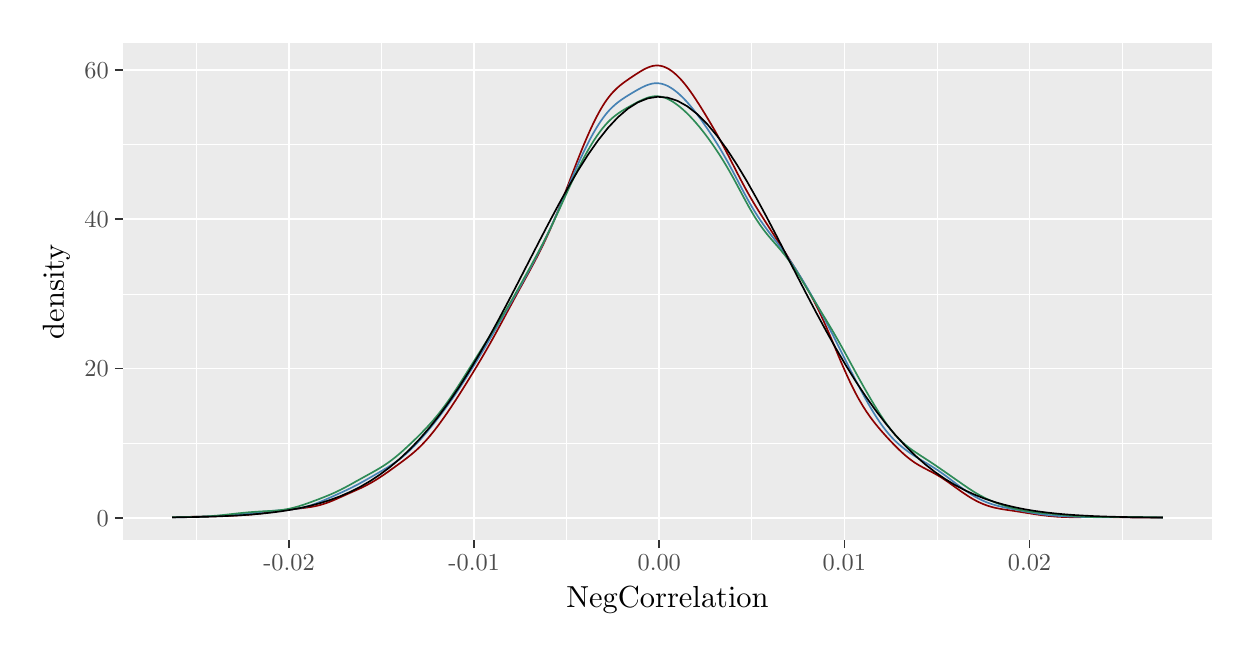
\begin{tikzpicture}[x=1pt,y=1pt]
\definecolor{fillColor}{RGB}{255,255,255}
\path[use as bounding box,fill=fillColor,fill opacity=0.00] (0,0) rectangle (433.62,216.81);
\begin{scope}
\path[clip] (  0.00,  0.00) rectangle (433.62,216.81);
\definecolor{drawColor}{RGB}{255,255,255}
\definecolor{fillColor}{RGB}{255,255,255}

\path[draw=drawColor,line width= 0.6pt,line join=round,line cap=round,fill=fillColor] (  0.00,  0.00) rectangle (433.62,216.81);
\end{scope}
\begin{scope}
\path[clip] ( 34.27, 31.53) rectangle (428.12,211.31);
\definecolor{fillColor}{gray}{0.92}

\path[fill=fillColor] ( 34.27, 31.53) rectangle (428.12,211.31);
\definecolor{drawColor}{RGB}{255,255,255}

\path[draw=drawColor,line width= 0.3pt,line join=round] ( 34.27, 66.67) --
	(428.12, 66.67);

\path[draw=drawColor,line width= 0.3pt,line join=round] ( 34.27,120.60) --
	(428.12,120.60);

\path[draw=drawColor,line width= 0.3pt,line join=round] ( 34.27,174.54) --
	(428.12,174.54);

\path[draw=drawColor,line width= 0.3pt,line join=round] ( 61.01, 31.53) --
	( 61.01,211.31);

\path[draw=drawColor,line width= 0.3pt,line join=round] (127.90, 31.53) --
	(127.90,211.31);

\path[draw=drawColor,line width= 0.3pt,line join=round] (194.78, 31.53) --
	(194.78,211.31);

\path[draw=drawColor,line width= 0.3pt,line join=round] (261.67, 31.53) --
	(261.67,211.31);

\path[draw=drawColor,line width= 0.3pt,line join=round] (328.56, 31.53) --
	(328.56,211.31);

\path[draw=drawColor,line width= 0.3pt,line join=round] (395.45, 31.53) --
	(395.45,211.31);

\path[draw=drawColor,line width= 0.6pt,line join=round] ( 34.27, 39.70) --
	(428.12, 39.70);

\path[draw=drawColor,line width= 0.6pt,line join=round] ( 34.27, 93.64) --
	(428.12, 93.64);

\path[draw=drawColor,line width= 0.6pt,line join=round] ( 34.27,147.57) --
	(428.12,147.57);

\path[draw=drawColor,line width= 0.6pt,line join=round] ( 34.27,201.50) --
	(428.12,201.50);

\path[draw=drawColor,line width= 0.6pt,line join=round] ( 94.45, 31.53) --
	( 94.45,211.31);

\path[draw=drawColor,line width= 0.6pt,line join=round] (161.34, 31.53) --
	(161.34,211.31);

\path[draw=drawColor,line width= 0.6pt,line join=round] (228.23, 31.53) --
	(228.23,211.31);

\path[draw=drawColor,line width= 0.6pt,line join=round] (295.12, 31.53) --
	(295.12,211.31);

\path[draw=drawColor,line width= 0.6pt,line join=round] (362.01, 31.53) --
	(362.01,211.31);
\definecolor{drawColor}{RGB}{139,0,0}

\path[draw=drawColor,line width= 0.6pt,line join=round] ( 52.17, 39.90) --
	( 52.87, 39.92) --
	( 53.57, 39.93) --
	( 54.27, 39.95) --
	( 54.97, 39.97) --
	( 55.67, 39.98) --
	( 56.37, 40.00) --
	( 57.07, 40.01) --
	( 57.78, 40.03) --
	( 58.48, 40.04) --
	( 59.18, 40.06) --
	( 59.88, 40.07) --
	( 60.58, 40.09) --
	( 61.28, 40.11) --
	( 61.98, 40.12) --
	( 62.68, 40.14) --
	( 63.38, 40.15) --
	( 64.08, 40.17) --
	( 64.78, 40.19) --
	( 65.48, 40.20) --
	( 66.18, 40.22) --
	( 66.88, 40.24) --
	( 67.59, 40.26) --
	( 68.29, 40.28) --
	( 68.99, 40.31) --
	( 69.69, 40.33) --
	( 70.39, 40.35) --
	( 71.09, 40.38) --
	( 71.79, 40.40) --
	( 72.49, 40.43) --
	( 73.19, 40.46) --
	( 73.89, 40.49) --
	( 74.59, 40.52) --
	( 75.29, 40.55) --
	( 75.99, 40.58) --
	( 76.69, 40.62) --
	( 77.39, 40.66) --
	( 78.10, 40.70) --
	( 78.80, 40.75) --
	( 79.50, 40.80) --
	( 80.20, 40.85) --
	( 80.90, 40.91) --
	( 81.60, 40.98) --
	( 82.30, 41.05) --
	( 83.00, 41.12) --
	( 83.70, 41.20) --
	( 84.40, 41.29) --
	( 85.10, 41.38) --
	( 85.80, 41.47) --
	( 86.50, 41.57) --
	( 87.20, 41.67) --
	( 87.90, 41.77) --
	( 88.61, 41.87) --
	( 89.31, 41.97) --
	( 90.01, 42.07) --
	( 90.71, 42.17) --
	( 91.41, 42.27) --
	( 92.11, 42.37) --
	( 92.81, 42.46) --
	( 93.51, 42.55) --
	( 94.21, 42.64) --
	( 94.91, 42.72) --
	( 95.61, 42.80) --
	( 96.31, 42.88) --
	( 97.01, 42.96) --
	( 97.71, 43.03) --
	( 98.42, 43.11) --
	( 99.12, 43.19) --
	( 99.82, 43.27) --
	(100.52, 43.35) --
	(101.22, 43.45) --
	(101.92, 43.55) --
	(102.62, 43.66) --
	(103.32, 43.79) --
	(104.02, 43.93) --
	(104.72, 44.09) --
	(105.42, 44.26) --
	(106.12, 44.45) --
	(106.82, 44.67) --
	(107.52, 44.89) --
	(108.22, 45.14) --
	(108.93, 45.41) --
	(109.63, 45.68) --
	(110.33, 45.97) --
	(111.03, 46.27) --
	(111.73, 46.57) --
	(112.43, 46.89) --
	(113.13, 47.20) --
	(113.83, 47.51) --
	(114.53, 47.83) --
	(115.23, 48.14) --
	(115.93, 48.45) --
	(116.63, 48.77) --
	(117.33, 49.08) --
	(118.03, 49.39) --
	(118.73, 49.70) --
	(119.44, 50.02) --
	(120.14, 50.34) --
	(120.84, 50.67) --
	(121.54, 51.01) --
	(122.24, 51.36) --
	(122.94, 51.73) --
	(123.64, 52.11) --
	(124.34, 52.50) --
	(125.04, 52.91) --
	(125.74, 53.33) --
	(126.44, 53.77) --
	(127.14, 54.22) --
	(127.84, 54.69) --
	(128.54, 55.16) --
	(129.24, 55.64) --
	(129.95, 56.13) --
	(130.65, 56.63) --
	(131.35, 57.13) --
	(132.05, 57.63) --
	(132.75, 58.14) --
	(133.45, 58.65) --
	(134.15, 59.16) --
	(134.85, 59.67) --
	(135.55, 60.19) --
	(136.25, 60.72) --
	(136.95, 61.25) --
	(137.65, 61.80) --
	(138.35, 62.36) --
	(139.05, 62.94) --
	(139.76, 63.54) --
	(140.46, 64.16) --
	(141.16, 64.81) --
	(141.86, 65.49) --
	(142.56, 66.19) --
	(143.26, 66.92) --
	(143.96, 67.68) --
	(144.66, 68.47) --
	(145.36, 69.29) --
	(146.06, 70.14) --
	(146.76, 71.01) --
	(147.46, 71.91) --
	(148.16, 72.83) --
	(148.86, 73.77) --
	(149.56, 74.74) --
	(150.27, 75.72) --
	(150.97, 76.71) --
	(151.67, 77.73) --
	(152.37, 78.76) --
	(153.07, 79.80) --
	(153.77, 80.86) --
	(154.47, 81.93) --
	(155.17, 83.01) --
	(155.87, 84.10) --
	(156.57, 85.21) --
	(157.27, 86.32) --
	(157.97, 87.44) --
	(158.67, 88.56) --
	(159.37, 89.70) --
	(160.07, 90.84) --
	(160.78, 91.98) --
	(161.48, 93.14) --
	(162.18, 94.29) --
	(162.88, 95.46) --
	(163.58, 96.63) --
	(164.28, 97.82) --
	(164.98, 99.02) --
	(165.68,100.22) --
	(166.38,101.45) --
	(167.08,102.68) --
	(167.78,103.93) --
	(168.48,105.19) --
	(169.18,106.46) --
	(169.88,107.75) --
	(170.59,109.05) --
	(171.29,110.35) --
	(171.99,111.66) --
	(172.69,112.97) --
	(173.39,114.28) --
	(174.09,115.58) --
	(174.79,116.88) --
	(175.49,118.18) --
	(176.19,119.47) --
	(176.89,120.76) --
	(177.59,122.04) --
	(178.29,123.31) --
	(178.99,124.58) --
	(179.69,125.86) --
	(180.39,127.13) --
	(181.10,128.42) --
	(181.80,129.71) --
	(182.50,131.02) --
	(183.20,132.34) --
	(183.90,133.68) --
	(184.60,135.05) --
	(185.30,136.44) --
	(186.00,137.86) --
	(186.70,139.31) --
	(187.40,140.80) --
	(188.10,142.33) --
	(188.80,143.90) --
	(189.50,145.51) --
	(190.20,147.15) --
	(190.90,148.83) --
	(191.61,150.55) --
	(192.31,152.30) --
	(193.01,154.08) --
	(193.71,155.89) --
	(194.41,157.71) --
	(195.11,159.54) --
	(195.81,161.38) --
	(196.51,163.22) --
	(197.21,165.05) --
	(197.91,166.86) --
	(198.61,168.66) --
	(199.31,170.44) --
	(200.01,172.18) --
	(200.71,173.90) --
	(201.42,175.58) --
	(202.12,177.22) --
	(202.82,178.82) --
	(203.52,180.37) --
	(204.22,181.86) --
	(204.92,183.30) --
	(205.62,184.67) --
	(206.32,185.99) --
	(207.02,187.24) --
	(207.72,188.42) --
	(208.42,189.53) --
	(209.12,190.56) --
	(209.82,191.51) --
	(210.52,192.39) --
	(211.22,193.21) --
	(211.93,193.96) --
	(212.63,194.66) --
	(213.33,195.30) --
	(214.03,195.90) --
	(214.73,196.46) --
	(215.43,196.98) --
	(216.13,197.49) --
	(216.83,197.98) --
	(217.53,198.46) --
	(218.23,198.93) --
	(218.93,199.40) --
	(219.63,199.86) --
	(220.33,200.31) --
	(221.03,200.75) --
	(221.73,201.18) --
	(222.44,201.58) --
	(223.14,201.95) --
	(223.84,202.28) --
	(224.54,202.57) --
	(225.24,202.81) --
	(225.94,202.99) --
	(226.64,203.10) --
	(227.34,203.14) --
	(228.04,203.11) --
	(228.74,203.01) --
	(229.44,202.84) --
	(230.14,202.60) --
	(230.84,202.30) --
	(231.54,201.92) --
	(232.24,201.47) --
	(232.95,200.97) --
	(233.65,200.41) --
	(234.35,199.79) --
	(235.05,199.12) --
	(235.75,198.40) --
	(236.45,197.63) --
	(237.15,196.81) --
	(237.85,195.94) --
	(238.55,195.02) --
	(239.25,194.07) --
	(239.95,193.08) --
	(240.65,192.05) --
	(241.35,191.00) --
	(242.05,189.92) --
	(242.76,188.82) --
	(243.46,187.71) --
	(244.16,186.57) --
	(244.86,185.43) --
	(245.56,184.27) --
	(246.26,183.10) --
	(246.96,181.92) --
	(247.66,180.72) --
	(248.36,179.51) --
	(249.06,178.27) --
	(249.76,177.02) --
	(250.46,175.74) --
	(251.16,174.44) --
	(251.86,173.13) --
	(252.56,171.79) --
	(253.27,170.44) --
	(253.97,169.07) --
	(254.67,167.70) --
	(255.37,166.33) --
	(256.07,164.96) --
	(256.77,163.60) --
	(257.47,162.25) --
	(258.17,160.92) --
	(258.87,159.61) --
	(259.57,158.32) --
	(260.27,157.07) --
	(260.97,155.84) --
	(261.67,154.63) --
	(262.37,153.44) --
	(263.07,152.28) --
	(263.78,151.14) --
	(264.48,150.01) --
	(265.18,148.89) --
	(265.88,147.79) --
	(266.58,146.69) --
	(267.28,145.60) --
	(267.98,144.51) --
	(268.68,143.42) --
	(269.38,142.33) --
	(270.08,141.23) --
	(270.78,140.14) --
	(271.48,139.04) --
	(272.18,137.94) --
	(272.88,136.83) --
	(273.59,135.73) --
	(274.29,134.62) --
	(274.99,133.51) --
	(275.69,132.39) --
	(276.39,131.28) --
	(277.09,130.15) --
	(277.79,129.03) --
	(278.49,127.89) --
	(279.19,126.74) --
	(279.89,125.58) --
	(280.59,124.40) --
	(281.29,123.20) --
	(281.99,121.98) --
	(282.69,120.72) --
	(283.39,119.42) --
	(284.10,118.09) --
	(284.80,116.72) --
	(285.50,115.31) --
	(286.20,113.86) --
	(286.90,112.37) --
	(287.60,110.84) --
	(288.30,109.26) --
	(289.00,107.66) --
	(289.70,106.03) --
	(290.40,104.38) --
	(291.10,102.71) --
	(291.80,101.04) --
	(292.50, 99.36) --
	(293.20, 97.69) --
	(293.90, 96.04) --
	(294.61, 94.42) --
	(295.31, 92.82) --
	(296.01, 91.25) --
	(296.71, 89.73) --
	(297.41, 88.24) --
	(298.11, 86.81) --
	(298.81, 85.42) --
	(299.51, 84.09) --
	(300.21, 82.81) --
	(300.91, 81.59) --
	(301.61, 80.41) --
	(302.31, 79.28) --
	(303.01, 78.20) --
	(303.71, 77.17) --
	(304.41, 76.18) --
	(305.12, 75.23) --
	(305.82, 74.31) --
	(306.52, 73.43) --
	(307.22, 72.58) --
	(307.92, 71.74) --
	(308.62, 70.93) --
	(309.32, 70.14) --
	(310.02, 69.36) --
	(310.72, 68.59) --
	(311.42, 67.84) --
	(312.12, 67.10) --
	(312.82, 66.37) --
	(313.52, 65.65) --
	(314.22, 64.95) --
	(314.93, 64.26) --
	(315.63, 63.60) --
	(316.33, 62.95) --
	(317.03, 62.33) --
	(317.73, 61.74) --
	(318.43, 61.18) --
	(319.13, 60.64) --
	(319.83, 60.13) --
	(320.53, 59.65) --
	(321.23, 59.20) --
	(321.93, 58.78) --
	(322.63, 58.37) --
	(323.33, 57.99) --
	(324.03, 57.61) --
	(324.73, 57.25) --
	(325.44, 56.89) --
	(326.14, 56.53) --
	(326.84, 56.16) --
	(327.54, 55.78) --
	(328.24, 55.39) --
	(328.94, 54.99) --
	(329.64, 54.57) --
	(330.34, 54.13) --
	(331.04, 53.67) --
	(331.74, 53.21) --
	(332.44, 52.72) --
	(333.14, 52.23) --
	(333.84, 51.72) --
	(334.54, 51.22) --
	(335.24, 50.71) --
	(335.95, 50.20) --
	(336.65, 49.70) --
	(337.35, 49.20) --
	(338.05, 48.71) --
	(338.75, 48.24) --
	(339.45, 47.78) --
	(340.15, 47.33) --
	(340.85, 46.90) --
	(341.55, 46.49) --
	(342.25, 46.10) --
	(342.95, 45.73) --
	(343.65, 45.38) --
	(344.35, 45.06) --
	(345.05, 44.76) --
	(345.76, 44.48) --
	(346.46, 44.22) --
	(347.16, 43.98) --
	(347.86, 43.77) --
	(348.56, 43.57) --
	(349.26, 43.39) --
	(349.96, 43.23) --
	(350.66, 43.09) --
	(351.36, 42.95) --
	(352.06, 42.83) --
	(352.76, 42.72) --
	(353.46, 42.61) --
	(354.16, 42.50) --
	(354.86, 42.40) --
	(355.56, 42.30) --
	(356.27, 42.20) --
	(356.97, 42.09) --
	(357.67, 41.99) --
	(358.37, 41.88) --
	(359.07, 41.77) --
	(359.77, 41.66) --
	(360.47, 41.55) --
	(361.17, 41.44) --
	(361.87, 41.33) --
	(362.57, 41.22) --
	(363.27, 41.11) --
	(363.97, 41.00) --
	(364.67, 40.90) --
	(365.37, 40.80) --
	(366.07, 40.70) --
	(366.78, 40.61) --
	(367.48, 40.53) --
	(368.18, 40.45) --
	(368.88, 40.37) --
	(369.58, 40.30) --
	(370.28, 40.23) --
	(370.98, 40.18) --
	(371.68, 40.12) --
	(372.38, 40.08) --
	(373.08, 40.04) --
	(373.78, 40.00) --
	(374.48, 39.98) --
	(375.18, 39.95) --
	(375.88, 39.94) --
	(376.58, 39.92) --
	(377.29, 39.92) --
	(377.99, 39.91) --
	(378.69, 39.92) --
	(379.39, 39.92) --
	(380.09, 39.92) --
	(380.79, 39.93) --
	(381.49, 39.94) --
	(382.19, 39.95) --
	(382.89, 39.95) --
	(383.59, 39.96) --
	(384.29, 39.97) --
	(384.99, 39.97) --
	(385.69, 39.97) --
	(386.39, 39.97) --
	(387.10, 39.97) --
	(387.80, 39.97) --
	(388.50, 39.97) --
	(389.20, 39.96) --
	(389.90, 39.95) --
	(390.60, 39.94) --
	(391.30, 39.94) --
	(392.00, 39.93) --
	(392.70, 39.92) --
	(393.40, 39.91) --
	(394.10, 39.90) --
	(394.80, 39.89) --
	(395.50, 39.87) --
	(396.20, 39.86) --
	(396.90, 39.86) --
	(397.61, 39.85) --
	(398.31, 39.84) --
	(399.01, 39.83) --
	(399.71, 39.83) --
	(400.41, 39.82) --
	(401.11, 39.82) --
	(401.81, 39.81) --
	(402.51, 39.81) --
	(403.21, 39.81) --
	(403.91, 39.81) --
	(404.61, 39.81) --
	(405.31, 39.81) --
	(406.01, 39.82) --
	(406.71, 39.82) --
	(407.41, 39.82) --
	(408.12, 39.82) --
	(408.82, 39.82) --
	(409.52, 39.82) --
	(410.22, 39.82);
\definecolor{drawColor}{RGB}{70,130,180}

\path[draw=drawColor,line width= 0.6pt,line join=round] ( 52.17, 39.85) --
	( 52.87, 39.86) --
	( 53.57, 39.87) --
	( 54.27, 39.88) --
	( 54.97, 39.90) --
	( 55.67, 39.91) --
	( 56.37, 39.92) --
	( 57.07, 39.94) --
	( 57.78, 39.95) --
	( 58.48, 39.97) --
	( 59.18, 39.99) --
	( 59.88, 40.02) --
	( 60.58, 40.04) --
	( 61.28, 40.07) --
	( 61.98, 40.09) --
	( 62.68, 40.12) --
	( 63.38, 40.15) --
	( 64.08, 40.18) --
	( 64.78, 40.21) --
	( 65.48, 40.25) --
	( 66.18, 40.28) --
	( 66.88, 40.31) --
	( 67.59, 40.35) --
	( 68.29, 40.38) --
	( 68.99, 40.42) --
	( 69.69, 40.46) --
	( 70.39, 40.50) --
	( 71.09, 40.54) --
	( 71.79, 40.58) --
	( 72.49, 40.63) --
	( 73.19, 40.67) --
	( 73.89, 40.73) --
	( 74.59, 40.78) --
	( 75.29, 40.84) --
	( 75.99, 40.90) --
	( 76.69, 40.97) --
	( 77.39, 41.04) --
	( 78.10, 41.11) --
	( 78.80, 41.18) --
	( 79.50, 41.26) --
	( 80.20, 41.34) --
	( 80.90, 41.42) --
	( 81.60, 41.50) --
	( 82.30, 41.58) --
	( 83.00, 41.66) --
	( 83.70, 41.74) --
	( 84.40, 41.81) --
	( 85.10, 41.89) --
	( 85.80, 41.96) --
	( 86.50, 42.03) --
	( 87.20, 42.09) --
	( 87.90, 42.15) --
	( 88.61, 42.21) --
	( 89.31, 42.26) --
	( 90.01, 42.31) --
	( 90.71, 42.36) --
	( 91.41, 42.41) --
	( 92.11, 42.46) --
	( 92.81, 42.51) --
	( 93.51, 42.57) --
	( 94.21, 42.63) --
	( 94.91, 42.70) --
	( 95.61, 42.77) --
	( 96.31, 42.86) --
	( 97.01, 42.96) --
	( 97.71, 43.08) --
	( 98.42, 43.21) --
	( 99.12, 43.35) --
	( 99.82, 43.51) --
	(100.52, 43.69) --
	(101.22, 43.89) --
	(101.92, 44.10) --
	(102.62, 44.33) --
	(103.32, 44.57) --
	(104.02, 44.82) --
	(104.72, 45.09) --
	(105.42, 45.37) --
	(106.12, 45.65) --
	(106.82, 45.95) --
	(107.52, 46.25) --
	(108.22, 46.55) --
	(108.93, 46.86) --
	(109.63, 47.17) --
	(110.33, 47.48) --
	(111.03, 47.80) --
	(111.73, 48.11) --
	(112.43, 48.43) --
	(113.13, 48.75) --
	(113.83, 49.07) --
	(114.53, 49.39) --
	(115.23, 49.72) --
	(115.93, 50.05) --
	(116.63, 50.39) --
	(117.33, 50.74) --
	(118.03, 51.10) --
	(118.73, 51.46) --
	(119.44, 51.83) --
	(120.14, 52.21) --
	(120.84, 52.60) --
	(121.54, 52.99) --
	(122.24, 53.38) --
	(122.94, 53.78) --
	(123.64, 54.18) --
	(124.34, 54.58) --
	(125.04, 54.98) --
	(125.74, 55.38) --
	(126.44, 55.79) --
	(127.14, 56.19) --
	(127.84, 56.60) --
	(128.54, 57.02) --
	(129.24, 57.44) --
	(129.95, 57.86) --
	(130.65, 58.30) --
	(131.35, 58.75) --
	(132.05, 59.21) --
	(132.75, 59.69) --
	(133.45, 60.18) --
	(134.15, 60.70) --
	(134.85, 61.25) --
	(135.55, 61.81) --
	(136.25, 62.40) --
	(136.95, 63.01) --
	(137.65, 63.64) --
	(138.35, 64.30) --
	(139.05, 64.99) --
	(139.76, 65.69) --
	(140.46, 66.42) --
	(141.16, 67.17) --
	(141.86, 67.94) --
	(142.56, 68.73) --
	(143.26, 69.53) --
	(143.96, 70.35) --
	(144.66, 71.19) --
	(145.36, 72.04) --
	(146.06, 72.90) --
	(146.76, 73.77) --
	(147.46, 74.66) --
	(148.16, 75.56) --
	(148.86, 76.47) --
	(149.56, 77.39) --
	(150.27, 78.33) --
	(150.97, 79.28) --
	(151.67, 80.24) --
	(152.37, 81.22) --
	(153.07, 82.21) --
	(153.77, 83.22) --
	(154.47, 84.24) --
	(155.17, 85.28) --
	(155.87, 86.33) --
	(156.57, 87.39) --
	(157.27, 88.47) --
	(157.97, 89.55) --
	(158.67, 90.65) --
	(159.37, 91.75) --
	(160.07, 92.87) --
	(160.78, 93.99) --
	(161.48, 95.12) --
	(162.18, 96.25) --
	(162.88, 97.40) --
	(163.58, 98.55) --
	(164.28, 99.71) --
	(164.98,100.88) --
	(165.68,102.05) --
	(166.38,103.23) --
	(167.08,104.42) --
	(167.78,105.61) --
	(168.48,106.81) --
	(169.18,108.01) --
	(169.88,109.21) --
	(170.59,110.42) --
	(171.29,111.63) --
	(171.99,112.84) --
	(172.69,114.05) --
	(173.39,115.26) --
	(174.09,116.48) --
	(174.79,117.69) --
	(175.49,118.91) --
	(176.19,120.14) --
	(176.89,121.37) --
	(177.59,122.61) --
	(178.29,123.86) --
	(178.99,125.11) --
	(179.69,126.37) --
	(180.39,127.64) --
	(181.10,128.93) --
	(181.80,130.22) --
	(182.50,131.53) --
	(183.20,132.85) --
	(183.90,134.19) --
	(184.60,135.55) --
	(185.30,136.93) --
	(186.00,138.33) --
	(186.70,139.75) --
	(187.40,141.20) --
	(188.10,142.68) --
	(188.80,144.19) --
	(189.50,145.73) --
	(190.20,147.29) --
	(190.90,148.88) --
	(191.61,150.49) --
	(192.31,152.13) --
	(193.01,153.78) --
	(193.71,155.44) --
	(194.41,157.10) --
	(195.11,158.77) --
	(195.81,160.43) --
	(196.51,162.09) --
	(197.21,163.72) --
	(197.91,165.34) --
	(198.61,166.93) --
	(199.31,168.49) --
	(200.01,170.02) --
	(200.71,171.51) --
	(201.42,172.97) --
	(202.12,174.38) --
	(202.82,175.75) --
	(203.52,177.08) --
	(204.22,178.36) --
	(204.92,179.58) --
	(205.62,180.75) --
	(206.32,181.87) --
	(207.02,182.93) --
	(207.72,183.93) --
	(208.42,184.87) --
	(209.12,185.76) --
	(209.82,186.58) --
	(210.52,187.34) --
	(211.22,188.04) --
	(211.93,188.69) --
	(212.63,189.30) --
	(213.33,189.86) --
	(214.03,190.39) --
	(214.73,190.89) --
	(215.43,191.36) --
	(216.13,191.81) --
	(216.83,192.25) --
	(217.53,192.68) --
	(218.23,193.10) --
	(218.93,193.52) --
	(219.63,193.93) --
	(220.33,194.33) --
	(221.03,194.72) --
	(221.73,195.09) --
	(222.44,195.44) --
	(223.14,195.76) --
	(223.84,196.05) --
	(224.54,196.29) --
	(225.24,196.49) --
	(225.94,196.64) --
	(226.64,196.72) --
	(227.34,196.74) --
	(228.04,196.70) --
	(228.74,196.60) --
	(229.44,196.44) --
	(230.14,196.21) --
	(230.84,195.93) --
	(231.54,195.59) --
	(232.24,195.18) --
	(232.95,194.73) --
	(233.65,194.24) --
	(234.35,193.69) --
	(235.05,193.11) --
	(235.75,192.49) --
	(236.45,191.82) --
	(237.15,191.12) --
	(237.85,190.38) --
	(238.55,189.61) --
	(239.25,188.80) --
	(239.95,187.96) --
	(240.65,187.09) --
	(241.35,186.20) --
	(242.05,185.28) --
	(242.76,184.33) --
	(243.46,183.37) --
	(244.16,182.38) --
	(244.86,181.37) --
	(245.56,180.35) --
	(246.26,179.31) --
	(246.96,178.25) --
	(247.66,177.18) --
	(248.36,176.08) --
	(249.06,174.96) --
	(249.76,173.82) --
	(250.46,172.65) --
	(251.16,171.45) --
	(251.86,170.23) --
	(252.56,168.99) --
	(253.27,167.72) --
	(253.97,166.42) --
	(254.67,165.11) --
	(255.37,163.78) --
	(256.07,162.45) --
	(256.77,161.11) --
	(257.47,159.77) --
	(258.17,158.44) --
	(258.87,157.12) --
	(259.57,155.83) --
	(260.27,154.56) --
	(260.97,153.32) --
	(261.67,152.11) --
	(262.37,150.94) --
	(263.07,149.80) --
	(263.78,148.70) --
	(264.48,147.64) --
	(265.18,146.61) --
	(265.88,145.61) --
	(266.58,144.64) --
	(267.28,143.69) --
	(267.98,142.76) --
	(268.68,141.84) --
	(269.38,140.93) --
	(270.08,140.02) --
	(270.78,139.10) --
	(271.48,138.18) --
	(272.18,137.25) --
	(272.88,136.30) --
	(273.59,135.34) --
	(274.29,134.35) --
	(274.99,133.35) --
	(275.69,132.32) --
	(276.39,131.28) --
	(277.09,130.21) --
	(277.79,129.13) --
	(278.49,128.02) --
	(279.19,126.90) --
	(279.89,125.76) --
	(280.59,124.60) --
	(281.29,123.43) --
	(281.99,122.24) --
	(282.69,121.03) --
	(283.39,119.81) --
	(284.10,118.58) --
	(284.80,117.33) --
	(285.50,116.06) --
	(286.20,114.78) --
	(286.90,113.49) --
	(287.60,112.18) --
	(288.30,110.86) --
	(289.00,109.52) --
	(289.70,108.17) --
	(290.40,106.81) --
	(291.10,105.44) --
	(291.80,104.06) --
	(292.50,102.67) --
	(293.20,101.28) --
	(293.90, 99.88) --
	(294.61, 98.48) --
	(295.31, 97.07) --
	(296.01, 95.68) --
	(296.71, 94.28) --
	(297.41, 92.89) --
	(298.11, 91.51) --
	(298.81, 90.14) --
	(299.51, 88.79) --
	(300.21, 87.44) --
	(300.91, 86.11) --
	(301.61, 84.80) --
	(302.31, 83.51) --
	(303.01, 82.25) --
	(303.71, 81.00) --
	(304.41, 79.79) --
	(305.12, 78.61) --
	(305.82, 77.45) --
	(306.52, 76.34) --
	(307.22, 75.26) --
	(307.92, 74.22) --
	(308.62, 73.23) --
	(309.32, 72.28) --
	(310.02, 71.37) --
	(310.72, 70.50) --
	(311.42, 69.68) --
	(312.12, 68.89) --
	(312.82, 68.15) --
	(313.52, 67.45) --
	(314.22, 66.79) --
	(314.93, 66.15) --
	(315.63, 65.55) --
	(316.33, 64.98) --
	(317.03, 64.43) --
	(317.73, 63.91) --
	(318.43, 63.41) --
	(319.13, 62.92) --
	(319.83, 62.46) --
	(320.53, 62.00) --
	(321.23, 61.56) --
	(321.93, 61.13) --
	(322.63, 60.71) --
	(323.33, 60.29) --
	(324.03, 59.87) --
	(324.73, 59.46) --
	(325.44, 59.04) --
	(326.14, 58.61) --
	(326.84, 58.18) --
	(327.54, 57.74) --
	(328.24, 57.29) --
	(328.94, 56.83) --
	(329.64, 56.35) --
	(330.34, 55.86) --
	(331.04, 55.36) --
	(331.74, 54.85) --
	(332.44, 54.33) --
	(333.14, 53.81) --
	(333.84, 53.28) --
	(334.54, 52.74) --
	(335.24, 52.21) --
	(335.95, 51.68) --
	(336.65, 51.15) --
	(337.35, 50.63) --
	(338.05, 50.13) --
	(338.75, 49.63) --
	(339.45, 49.15) --
	(340.15, 48.68) --
	(340.85, 48.24) --
	(341.55, 47.81) --
	(342.25, 47.40) --
	(342.95, 47.01) --
	(343.65, 46.63) --
	(344.35, 46.28) --
	(345.05, 45.95) --
	(345.76, 45.64) --
	(346.46, 45.35) --
	(347.16, 45.08) --
	(347.86, 44.83) --
	(348.56, 44.60) --
	(349.26, 44.38) --
	(349.96, 44.18) --
	(350.66, 43.99) --
	(351.36, 43.82) --
	(352.06, 43.65) --
	(352.76, 43.49) --
	(353.46, 43.34) --
	(354.16, 43.20) --
	(354.86, 43.06) --
	(355.56, 42.92) --
	(356.27, 42.78) --
	(356.97, 42.65) --
	(357.67, 42.51) --
	(358.37, 42.38) --
	(359.07, 42.24) --
	(359.77, 42.11) --
	(360.47, 41.97) --
	(361.17, 41.84) --
	(361.87, 41.71) --
	(362.57, 41.58) --
	(363.27, 41.46) --
	(363.97, 41.34) --
	(364.67, 41.22) --
	(365.37, 41.11) --
	(366.07, 41.01) --
	(366.78, 40.92) --
	(367.48, 40.83) --
	(368.18, 40.75) --
	(368.88, 40.67) --
	(369.58, 40.60) --
	(370.28, 40.54) --
	(370.98, 40.48) --
	(371.68, 40.43) --
	(372.38, 40.38) --
	(373.08, 40.34) --
	(373.78, 40.30) --
	(374.48, 40.26) --
	(375.18, 40.22) --
	(375.88, 40.19) --
	(376.58, 40.16) --
	(377.29, 40.13) --
	(377.99, 40.11) --
	(378.69, 40.08) --
	(379.39, 40.06) --
	(380.09, 40.04) --
	(380.79, 40.01) --
	(381.49, 40.00) --
	(382.19, 39.98) --
	(382.89, 39.96) --
	(383.59, 39.95) --
	(384.29, 39.94) --
	(384.99, 39.93) --
	(385.69, 39.92) --
	(386.39, 39.92) --
	(387.10, 39.92) --
	(387.80, 39.92) --
	(388.50, 39.92) --
	(389.20, 39.92) --
	(389.90, 39.92) --
	(390.60, 39.92) --
	(391.30, 39.92) --
	(392.00, 39.93) --
	(392.70, 39.93) --
	(393.40, 39.93) --
	(394.10, 39.93) --
	(394.80, 39.93) --
	(395.50, 39.93) --
	(396.20, 39.92) --
	(396.90, 39.92) --
	(397.61, 39.92) --
	(398.31, 39.91) --
	(399.01, 39.91) --
	(399.71, 39.90) --
	(400.41, 39.90) --
	(401.11, 39.89) --
	(401.81, 39.89) --
	(402.51, 39.88) --
	(403.21, 39.87) --
	(403.91, 39.87) --
	(404.61, 39.86) --
	(405.31, 39.86) --
	(406.01, 39.86) --
	(406.71, 39.85) --
	(407.41, 39.85) --
	(408.12, 39.84) --
	(408.82, 39.83) --
	(409.52, 39.83) --
	(410.22, 39.82);
\definecolor{drawColor}{RGB}{46,139,87}

\path[draw=drawColor,line width= 0.6pt,line join=round] ( 52.17, 39.91) --
	( 52.87, 39.92) --
	( 53.57, 39.93) --
	( 54.27, 39.95) --
	( 54.97, 39.96) --
	( 55.67, 39.97) --
	( 56.37, 39.98) --
	( 57.07, 39.99) --
	( 57.78, 40.01) --
	( 58.48, 40.02) --
	( 59.18, 40.03) --
	( 59.88, 40.05) --
	( 60.58, 40.07) --
	( 61.28, 40.09) --
	( 61.98, 40.11) --
	( 62.68, 40.13) --
	( 63.38, 40.16) --
	( 64.08, 40.19) --
	( 64.78, 40.23) --
	( 65.48, 40.27) --
	( 66.18, 40.32) --
	( 66.88, 40.37) --
	( 67.59, 40.43) --
	( 68.29, 40.49) --
	( 68.99, 40.55) --
	( 69.69, 40.62) --
	( 70.39, 40.69) --
	( 71.09, 40.77) --
	( 71.79, 40.84) --
	( 72.49, 40.92) --
	( 73.19, 41.00) --
	( 73.89, 41.08) --
	( 74.59, 41.15) --
	( 75.29, 41.23) --
	( 75.99, 41.31) --
	( 76.69, 41.38) --
	( 77.39, 41.46) --
	( 78.10, 41.53) --
	( 78.80, 41.59) --
	( 79.50, 41.66) --
	( 80.20, 41.72) --
	( 80.90, 41.77) --
	( 81.60, 41.83) --
	( 82.30, 41.88) --
	( 83.00, 41.93) --
	( 83.70, 41.97) --
	( 84.40, 42.01) --
	( 85.10, 42.05) --
	( 85.80, 42.08) --
	( 86.50, 42.12) --
	( 87.20, 42.16) --
	( 87.90, 42.20) --
	( 88.61, 42.24) --
	( 89.31, 42.29) --
	( 90.01, 42.35) --
	( 90.71, 42.42) --
	( 91.41, 42.49) --
	( 92.11, 42.58) --
	( 92.81, 42.69) --
	( 93.51, 42.80) --
	( 94.21, 42.93) --
	( 94.91, 43.08) --
	( 95.61, 43.24) --
	( 96.31, 43.42) --
	( 97.01, 43.61) --
	( 97.71, 43.81) --
	( 98.42, 44.02) --
	( 99.12, 44.25) --
	( 99.82, 44.48) --
	(100.52, 44.72) --
	(101.22, 44.97) --
	(101.92, 45.22) --
	(102.62, 45.48) --
	(103.32, 45.74) --
	(104.02, 46.00) --
	(104.72, 46.26) --
	(105.42, 46.53) --
	(106.12, 46.80) --
	(106.82, 47.08) --
	(107.52, 47.36) --
	(108.22, 47.64) --
	(108.93, 47.93) --
	(109.63, 48.23) --
	(110.33, 48.54) --
	(111.03, 48.85) --
	(111.73, 49.18) --
	(112.43, 49.52) --
	(113.13, 49.86) --
	(113.83, 50.22) --
	(114.53, 50.59) --
	(115.23, 50.96) --
	(115.93, 51.34) --
	(116.63, 51.72) --
	(117.33, 52.11) --
	(118.03, 52.50) --
	(118.73, 52.90) --
	(119.44, 53.29) --
	(120.14, 53.68) --
	(120.84, 54.07) --
	(121.54, 54.45) --
	(122.24, 54.84) --
	(122.94, 55.23) --
	(123.64, 55.61) --
	(124.34, 56.00) --
	(125.04, 56.39) --
	(125.74, 56.79) --
	(126.44, 57.19) --
	(127.14, 57.61) --
	(127.84, 58.04) --
	(128.54, 58.48) --
	(129.24, 58.94) --
	(129.95, 59.42) --
	(130.65, 59.91) --
	(131.35, 60.43) --
	(132.05, 60.97) --
	(132.75, 61.52) --
	(133.45, 62.09) --
	(134.15, 62.68) --
	(134.85, 63.29) --
	(135.55, 63.90) --
	(136.25, 64.54) --
	(136.95, 65.18) --
	(137.65, 65.83) --
	(138.35, 66.49) --
	(139.05, 67.16) --
	(139.76, 67.83) --
	(140.46, 68.52) --
	(141.16, 69.21) --
	(141.86, 69.91) --
	(142.56, 70.62) --
	(143.26, 71.34) --
	(143.96, 72.08) --
	(144.66, 72.83) --
	(145.36, 73.60) --
	(146.06, 74.38) --
	(146.76, 75.19) --
	(147.46, 76.02) --
	(148.16, 76.88) --
	(148.86, 77.76) --
	(149.56, 78.66) --
	(150.27, 79.59) --
	(150.97, 80.54) --
	(151.67, 81.51) --
	(152.37, 82.51) --
	(153.07, 83.53) --
	(153.77, 84.56) --
	(154.47, 85.62) --
	(155.17, 86.69) --
	(155.87, 87.77) --
	(156.57, 88.86) --
	(157.27, 89.96) --
	(157.97, 91.07) --
	(158.67, 92.18) --
	(159.37, 93.30) --
	(160.07, 94.41) --
	(160.78, 95.53) --
	(161.48, 96.65) --
	(162.18, 97.77) --
	(162.88, 98.88) --
	(163.58, 99.99) --
	(164.28,101.10) --
	(164.98,102.21) --
	(165.68,103.31) --
	(166.38,104.42) --
	(167.08,105.52) --
	(167.78,106.63) --
	(168.48,107.74) --
	(169.18,108.86) --
	(169.88,109.99) --
	(170.59,111.12) --
	(171.29,112.26) --
	(171.99,113.42) --
	(172.69,114.58) --
	(173.39,115.77) --
	(174.09,116.96) --
	(174.79,118.16) --
	(175.49,119.38) --
	(176.19,120.61) --
	(176.89,121.85) --
	(177.59,123.09) --
	(178.29,124.35) --
	(178.99,125.61) --
	(179.69,126.87) --
	(180.39,128.14) --
	(181.10,129.41) --
	(181.80,130.69) --
	(182.50,131.97) --
	(183.20,133.26) --
	(183.90,134.56) --
	(184.60,135.87) --
	(185.30,137.19) --
	(186.00,138.53) --
	(186.70,139.89) --
	(187.40,141.27) --
	(188.10,142.68) --
	(188.80,144.11) --
	(189.50,145.56) --
	(190.20,147.04) --
	(190.90,148.54) --
	(191.61,150.06) --
	(192.31,151.59) --
	(193.01,153.13) --
	(193.71,154.68) --
	(194.41,156.23) --
	(195.11,157.77) --
	(195.81,159.30) --
	(196.51,160.81) --
	(197.21,162.30) --
	(197.91,163.77) --
	(198.61,165.21) --
	(199.31,166.62) --
	(200.01,167.99) --
	(200.71,169.32) --
	(201.42,170.62) --
	(202.12,171.89) --
	(202.82,173.11) --
	(203.52,174.30) --
	(204.22,175.44) --
	(204.92,176.54) --
	(205.62,177.58) --
	(206.32,178.58) --
	(207.02,179.53) --
	(207.72,180.43) --
	(208.42,181.28) --
	(209.12,182.07) --
	(209.82,182.82) --
	(210.52,183.50) --
	(211.22,184.13) --
	(211.93,184.72) --
	(212.63,185.27) --
	(213.33,185.78) --
	(214.03,186.26) --
	(214.73,186.72) --
	(215.43,187.15) --
	(216.13,187.56) --
	(216.83,187.97) --
	(217.53,188.36) --
	(218.23,188.75) --
	(218.93,189.13) --
	(219.63,189.51) --
	(220.33,189.88) --
	(221.03,190.23) --
	(221.73,190.57) --
	(222.44,190.89) --
	(223.14,191.18) --
	(223.84,191.44) --
	(224.54,191.66) --
	(225.24,191.83) --
	(225.94,191.96) --
	(226.64,192.03) --
	(227.34,192.04) --
	(228.04,191.99) --
	(228.74,191.89) --
	(229.44,191.73) --
	(230.14,191.51) --
	(230.84,191.24) --
	(231.54,190.92) --
	(232.24,190.55) --
	(232.95,190.14) --
	(233.65,189.68) --
	(234.35,189.19) --
	(235.05,188.67) --
	(235.75,188.11) --
	(236.45,187.52) --
	(237.15,186.90) --
	(237.85,186.25) --
	(238.55,185.56) --
	(239.25,184.86) --
	(239.95,184.12) --
	(240.65,183.36) --
	(241.35,182.57) --
	(242.05,181.75) --
	(242.76,180.91) --
	(243.46,180.04) --
	(244.16,179.15) --
	(244.86,178.24) --
	(245.56,177.30) --
	(246.26,176.35) --
	(246.96,175.37) --
	(247.66,174.38) --
	(248.36,173.36) --
	(249.06,172.31) --
	(249.76,171.25) --
	(250.46,170.15) --
	(251.16,169.04) --
	(251.86,167.89) --
	(252.56,166.72) --
	(253.27,165.51) --
	(253.97,164.28) --
	(254.67,163.03) --
	(255.37,161.76) --
	(256.07,160.47) --
	(256.77,159.16) --
	(257.47,157.85) --
	(258.17,156.54) --
	(258.87,155.23) --
	(259.57,153.94) --
	(260.27,152.67) --
	(260.97,151.42) --
	(261.67,150.21) --
	(262.37,149.03) --
	(263.07,147.90) --
	(263.78,146.82) --
	(264.48,145.78) --
	(265.18,144.79) --
	(265.88,143.84) --
	(266.58,142.93) --
	(267.28,142.05) --
	(267.98,141.21) --
	(268.68,140.39) --
	(269.38,139.59) --
	(270.08,138.79) --
	(270.78,137.99) --
	(271.48,137.18) --
	(272.18,136.35) --
	(272.88,135.50) --
	(273.59,134.63) --
	(274.29,133.72) --
	(274.99,132.77) --
	(275.69,131.79) --
	(276.39,130.78) --
	(277.09,129.74) --
	(277.79,128.67) --
	(278.49,127.58) --
	(279.19,126.46) --
	(279.89,125.32) --
	(280.59,124.18) --
	(281.29,123.02) --
	(281.99,121.87) --
	(282.69,120.71) --
	(283.39,119.55) --
	(284.10,118.40) --
	(284.80,117.25) --
	(285.50,116.10) --
	(286.20,114.96) --
	(286.90,113.81) --
	(287.60,112.67) --
	(288.30,111.52) --
	(289.00,110.36) --
	(289.70,109.20) --
	(290.40,108.02) --
	(291.10,106.83) --
	(291.80,105.62) --
	(292.50,104.40) --
	(293.20,103.17) --
	(293.90,101.92) --
	(294.61,100.66) --
	(295.31, 99.39) --
	(296.01, 98.11) --
	(296.71, 96.82) --
	(297.41, 95.53) --
	(298.11, 94.24) --
	(298.81, 92.96) --
	(299.51, 91.68) --
	(300.21, 90.40) --
	(300.91, 89.14) --
	(301.61, 87.89) --
	(302.31, 86.64) --
	(303.01, 85.42) --
	(303.71, 84.20) --
	(304.41, 83.00) --
	(305.12, 81.81) --
	(305.82, 80.64) --
	(306.52, 79.49) --
	(307.22, 78.37) --
	(307.92, 77.26) --
	(308.62, 76.18) --
	(309.32, 75.13) --
	(310.02, 74.12) --
	(310.72, 73.13) --
	(311.42, 72.19) --
	(312.12, 71.30) --
	(312.82, 70.44) --
	(313.52, 69.63) --
	(314.22, 68.86) --
	(314.93, 68.13) --
	(315.63, 67.44) --
	(316.33, 66.80) --
	(317.03, 66.20) --
	(317.73, 65.63) --
	(318.43, 65.08) --
	(319.13, 64.56) --
	(319.83, 64.06) --
	(320.53, 63.58) --
	(321.23, 63.11) --
	(321.93, 62.65) --
	(322.63, 62.19) --
	(323.33, 61.74) --
	(324.03, 61.28) --
	(324.73, 60.83) --
	(325.44, 60.37) --
	(326.14, 59.91) --
	(326.84, 59.44) --
	(327.54, 58.97) --
	(328.24, 58.50) --
	(328.94, 58.02) --
	(329.64, 57.54) --
	(330.34, 57.06) --
	(331.04, 56.58) --
	(331.74, 56.09) --
	(332.44, 55.60) --
	(333.14, 55.11) --
	(333.84, 54.62) --
	(334.54, 54.13) --
	(335.24, 53.64) --
	(335.95, 53.14) --
	(336.65, 52.65) --
	(337.35, 52.16) --
	(338.05, 51.68) --
	(338.75, 51.20) --
	(339.45, 50.72) --
	(340.15, 50.25) --
	(340.85, 49.80) --
	(341.55, 49.35) --
	(342.25, 48.91) --
	(342.95, 48.49) --
	(343.65, 48.09) --
	(344.35, 47.69) --
	(345.05, 47.32) --
	(345.76, 46.96) --
	(346.46, 46.61) --
	(347.16, 46.28) --
	(347.86, 45.97) --
	(348.56, 45.67) --
	(349.26, 45.38) --
	(349.96, 45.11) --
	(350.66, 44.84) --
	(351.36, 44.59) --
	(352.06, 44.35) --
	(352.76, 44.12) --
	(353.46, 43.90) --
	(354.16, 43.69) --
	(354.86, 43.48) --
	(355.56, 43.29) --
	(356.27, 43.11) --
	(356.97, 42.93) --
	(357.67, 42.77) --
	(358.37, 42.61) --
	(359.07, 42.47) --
	(359.77, 42.33) --
	(360.47, 42.21) --
	(361.17, 42.09) --
	(361.87, 41.98) --
	(362.57, 41.89) --
	(363.27, 41.79) --
	(363.97, 41.71) --
	(364.67, 41.63) --
	(365.37, 41.56) --
	(366.07, 41.49) --
	(366.78, 41.42) --
	(367.48, 41.35) --
	(368.18, 41.29) --
	(368.88, 41.22) --
	(369.58, 41.16) --
	(370.28, 41.10) --
	(370.98, 41.03) --
	(371.68, 40.97) --
	(372.38, 40.90) --
	(373.08, 40.83) --
	(373.78, 40.76) --
	(374.48, 40.70) --
	(375.18, 40.63) --
	(375.88, 40.56) --
	(376.58, 40.50) --
	(377.29, 40.44) --
	(377.99, 40.38) --
	(378.69, 40.32) --
	(379.39, 40.27) --
	(380.09, 40.22) --
	(380.79, 40.17) --
	(381.49, 40.13) --
	(382.19, 40.10) --
	(382.89, 40.06) --
	(383.59, 40.03) --
	(384.29, 40.01) --
	(384.99, 39.99) --
	(385.69, 39.97) --
	(386.39, 39.96) --
	(387.10, 39.95) --
	(387.80, 39.94) --
	(388.50, 39.94) --
	(389.20, 39.94) --
	(389.90, 39.94) --
	(390.60, 39.94) --
	(391.30, 39.94) --
	(392.00, 39.95) --
	(392.70, 39.95) --
	(393.40, 39.96) --
	(394.10, 39.97) --
	(394.80, 39.97) --
	(395.50, 39.98) --
	(396.20, 39.98) --
	(396.90, 39.99) --
	(397.61, 39.99) --
	(398.31, 39.99) --
	(399.01, 39.99) --
	(399.71, 39.99) --
	(400.41, 39.99) --
	(401.11, 39.98) --
	(401.81, 39.98) --
	(402.51, 39.97) --
	(403.21, 39.96) --
	(403.91, 39.95) --
	(404.61, 39.94) --
	(405.31, 39.93) --
	(406.01, 39.91) --
	(406.71, 39.90) --
	(407.41, 39.89) --
	(408.12, 39.87) --
	(408.82, 39.86) --
	(409.52, 39.84) --
	(410.22, 39.83);
\definecolor{drawColor}{RGB}{0,0,0}

\path[draw=drawColor,line width= 0.6pt,line join=round] ( 52.17, 39.85) --
	( 55.75, 39.90) --
	( 59.33, 39.96) --
	( 62.91, 40.04) --
	( 66.49, 40.14) --
	( 70.07, 40.27) --
	( 73.65, 40.43) --
	( 77.23, 40.63) --
	( 80.81, 40.89) --
	( 84.39, 41.20) --
	( 87.97, 41.58) --
	( 91.56, 42.04) --
	( 95.14, 42.61) --
	( 98.72, 43.28) --
	(102.30, 44.10) --
	(105.88, 45.06) --
	(109.46, 46.20) --
	(113.04, 47.54) --
	(116.62, 49.10) --
	(120.20, 50.91) --
	(123.78, 52.99) --
	(127.36, 55.36) --
	(130.94, 58.05) --
	(134.52, 61.08) --
	(138.10, 64.46) --
	(141.68, 68.22) --
	(145.26, 72.37) --
	(148.84, 76.90) --
	(152.42, 81.82) --
	(156.00, 87.12) --
	(159.58, 92.77) --
	(163.16, 98.77) --
	(166.75,105.06) --
	(170.33,111.62) --
	(173.91,118.37) --
	(177.49,125.27) --
	(181.07,132.25) --
	(184.65,139.22) --
	(188.23,146.10) --
	(191.81,152.81) --
	(195.39,159.26) --
	(198.97,165.35) --
	(202.55,171.00) --
	(206.13,176.11) --
	(209.71,180.62) --
	(213.29,184.45) --
	(216.87,187.52) --
	(220.45,189.80) --
	(224.03,191.25) --
	(227.61,191.83) --
	(231.19,191.55) --
	(234.77,190.40) --
	(238.35,188.40) --
	(241.94,185.59) --
	(245.52,182.01) --
	(249.10,177.73) --
	(252.68,172.82) --
	(256.26,167.34) --
	(259.84,161.40) --
	(263.42,155.06) --
	(267.00,148.43) --
	(270.58,141.60) --
	(274.16,134.65) --
	(277.74,127.66) --
	(281.32,120.73) --
	(284.90,113.92) --
	(288.48,107.29) --
	(292.06,100.90) --
	(295.64, 94.80) --
	(299.22, 89.02) --
	(302.80, 83.60) --
	(306.38, 78.55) --
	(309.96, 73.88) --
	(313.54, 69.60) --
	(317.13, 65.71) --
	(320.71, 62.20) --
	(324.29, 59.05) --
	(327.87, 56.24) --
	(331.45, 53.76) --
	(335.03, 51.59) --
	(338.61, 49.69) --
	(342.19, 48.05) --
	(345.77, 46.64) --
	(349.35, 45.43) --
	(352.93, 44.41) --
	(356.51, 43.55) --
	(360.09, 42.82) --
	(363.67, 42.22) --
	(367.25, 41.73) --
	(370.83, 41.32) --
	(374.41, 40.98) --
	(377.99, 40.71) --
	(381.57, 40.50) --
	(385.15, 40.32) --
	(388.73, 40.18) --
	(392.32, 40.07) --
	(395.90, 39.99) --
	(399.48, 39.92) --
	(403.06, 39.87) --
	(406.64, 39.83) --
	(410.22, 39.80);
\end{scope}
\begin{scope}
\path[clip] (  0.00,  0.00) rectangle (433.62,216.81);
\definecolor{drawColor}{gray}{0.30}

\node[text=drawColor,anchor=base east,inner sep=0pt, outer sep=0pt, scale=  0.88] at ( 29.32, 36.67) {0};

\node[text=drawColor,anchor=base east,inner sep=0pt, outer sep=0pt, scale=  0.88] at ( 29.32, 90.61) {20};

\node[text=drawColor,anchor=base east,inner sep=0pt, outer sep=0pt, scale=  0.88] at ( 29.32,144.54) {40};

\node[text=drawColor,anchor=base east,inner sep=0pt, outer sep=0pt, scale=  0.88] at ( 29.32,198.47) {60};
\end{scope}
\begin{scope}
\path[clip] (  0.00,  0.00) rectangle (433.62,216.81);
\definecolor{drawColor}{gray}{0.20}

\path[draw=drawColor,line width= 0.6pt,line join=round] ( 31.52, 39.70) --
	( 34.27, 39.70);

\path[draw=drawColor,line width= 0.6pt,line join=round] ( 31.52, 93.64) --
	( 34.27, 93.64);

\path[draw=drawColor,line width= 0.6pt,line join=round] ( 31.52,147.57) --
	( 34.27,147.57);

\path[draw=drawColor,line width= 0.6pt,line join=round] ( 31.52,201.50) --
	( 34.27,201.50);
\end{scope}
\begin{scope}
\path[clip] (  0.00,  0.00) rectangle (433.62,216.81);
\definecolor{drawColor}{gray}{0.20}

\path[draw=drawColor,line width= 0.6pt,line join=round] ( 94.45, 28.78) --
	( 94.45, 31.53);

\path[draw=drawColor,line width= 0.6pt,line join=round] (161.34, 28.78) --
	(161.34, 31.53);

\path[draw=drawColor,line width= 0.6pt,line join=round] (228.23, 28.78) --
	(228.23, 31.53);

\path[draw=drawColor,line width= 0.6pt,line join=round] (295.12, 28.78) --
	(295.12, 31.53);

\path[draw=drawColor,line width= 0.6pt,line join=round] (362.01, 28.78) --
	(362.01, 31.53);
\end{scope}
\begin{scope}
\path[clip] (  0.00,  0.00) rectangle (433.62,216.81);
\definecolor{drawColor}{gray}{0.30}

\node[text=drawColor,anchor=base,inner sep=0pt, outer sep=0pt, scale=  0.88] at ( 94.45, 20.52) {-0.02};

\node[text=drawColor,anchor=base,inner sep=0pt, outer sep=0pt, scale=  0.88] at (161.34, 20.52) {-0.01};

\node[text=drawColor,anchor=base,inner sep=0pt, outer sep=0pt, scale=  0.88] at (228.23, 20.52) {0.00};

\node[text=drawColor,anchor=base,inner sep=0pt, outer sep=0pt, scale=  0.88] at (295.12, 20.52) {0.01};

\node[text=drawColor,anchor=base,inner sep=0pt, outer sep=0pt, scale=  0.88] at (362.01, 20.52) {0.02};
\end{scope}
\begin{scope}
\path[clip] (  0.00,  0.00) rectangle (433.62,216.81);
\definecolor{drawColor}{RGB}{0,0,0}

\node[text=drawColor,anchor=base,inner sep=0pt, outer sep=0pt, scale=  1.10] at (231.19,  7.44) {NegCorrelation};
\end{scope}
\begin{scope}
\path[clip] (  0.00,  0.00) rectangle (433.62,216.81);
\definecolor{drawColor}{RGB}{0,0,0}

\node[text=drawColor,rotate= 90.00,anchor=base,inner sep=0pt, outer sep=0pt, scale=  1.10] at ( 13.08,121.42) {density};
\end{scope}
\end{tikzpicture}

\caption{Merton: Log--return skewness on Heston}
\floatfoot{The above densities function (red, blue and green) are constructed over three distinctive groups of 10000 samples each. The black curve density is theoretical.
All samples are generated by an algorithm based on \cref{eq:other:hsvstock} for the stock data and on \cref{eq:other:hsvvol} for the related volatility (see function \textit{heston()} on appendix \ref{sub:r:time:heston} for more information). The only parameter that changes over the groups is $\sigma$ which is set to 0, 0.2, 0.4. The log-return densities of these groups are respectively represented by the green, blue and red outlined density curves. 
The black density represents to the normal bell curve with mean $- \frac{\theta}{2}$ and standard deviation of $\sqrt{\theta}$. The log-price return cover a period of one year with a time step of 500.
}
\label{p:other:heston:kurtosis}
\end{figure}




%%%%%%%%%%%%%%%%%%%%%%%%%%%%%%%%%%%%%%%%%%%%%%%%
% SECTION: Option pricing method
%%%%%%%%%%%%%%%%%%%%%%%%%%%%%%%%%%%%%%%%%%%%%%%%
\section{Option pricing method}
\label{sec:other:option}

As shown by \cref{sec:other:merton} and \cref{sec:other:heston}, the frameworks developed by \citet{merton76} and \citet{heston1993} drastically change the distribution of any underlying assets following such processes. Therefore, the pricing method to be used must also be adapted in order to take that update into account.

In his paper, \citet{heston1993} developed a techinque to price options using the characteristic function of the underlying asset. Furthermore, according to \citet{criso2015} that method could be used to price every options provided that the underlying's characteristic  is known.


%%%%%%%%%%%%%%%%%%%%%%%%%%%%%%%%%%%%%%%%%%%%%%%%
% SUBSECTION: Probabilistic approach
%%%%%%%%%%%%%%%%%%%%%%%%%%%%%%%%%%%%%%%%%%%%%%%%
\subsection{Probabilistic approach}
\label{sub:other:option:probabilistic}

\citet{heston1993} proposed the solution given by \cref{eq:other:call:heston} to price a european call option.

\begin{align}
  C(t) = S(t) P_1 - e^{-r(T-t)} K P_2 \label{eq:other:call:heston}
\end{align}

Through this method, the european call price at time $t$, namely $C(t)$, is computed thanks to \cref{eq:other:call:heston}, where $S(t)$ and $e^{r(T - t)}$ respectively stand for the stock price and the present value of the strike at that time $t$.

\begin{align}
  P_1(x,V,t;\ln{K}) &= \frac{1}{2} + \frac{1}{\pi} \int_0^{\infty} Re \left( \frac{e^{-i\phi\ln{K}} \psi(x,V,t;\phi - i)}{i\phi\psi(x,V,t;-i)} \right) d\phi \label{eq:other:call:heston:pi1} \\ 
  \intertext{}
  P_2(x,V,t;\ln{K}) &= \frac{1}{2} + \frac{1}{\pi} \int_0^{\infty} Re \left( \frac{e^{-i\phi\ln{K}} \psi(x,V,t;\phi)}{i\phi} \right) d\phi \label{eq:other:call:heston:pi2}
\end{align}

Following the development in \citet{criso2015}, \Cref{eq:other:call:heston:pi} both are probability quantities that involve the underlying characteristic function, namely $\psi(x,V,t;\phi)$. Once these quantities are computed, they are substituted in \cref{eq:other:call:heston} in order to get the call price at time $t$.

The characteristic functions for the Merton jump--diffusion (\cref{sec:other:merton}) and Heston stochastic volatility (\cref{sec:other:heston}) models are developed \cref{sub:other:option:merton,sub:other:option:heston}



%%%%%%%%%%%%%%%%%%%%%%%%%%%%%%%%%%%%%%%%%%%%%%%%%%%%%%%%%%%%%%%%%%%%%%%%%%%%%%%%
% SUBSECTION: Characteristic function for Merton Mixed jump--diffusion model
%%%%%%%%%%%%%%%%%%%%%%%%%%%%%%%%%%%%%%%%%%%%%%%%%%%%%%%%%%%%%%%%%%%%%%%%%%%%%%%%
\subsection{Characteristic function for Merton Mixed jump--diffusion model}
\label{sub:other:option:merton}

\citet{matsuda2004} demonstrates that the characteristic function of the Merton mixed jump-diffusion process is given by \cref{eq:other:merton:psi}. The baseline equation to construct the Merton's process characteristic function is the risk-neutralized version, namely \cref{eq:other:merton:pde:riskneutral}.

\begin{align}
\psi^{merton}(\phi) &= e^{ 
  \lambda (T - t) \left( e^{i \mu \phi - \frac{\delta^2 \phi^2}{2}} - 1\right) +
  i \phi \left( \ln S(t) + \left(  r - \frac{\sigma^2}{2} - \lambda \kappa \right) (T - t) \right) -
  \sigma^2 \frac{\phi^2}{2} (T - t)
}
\label{eq:other:merton:psi} \\
\intertext{where}
\kappa &= e^{\mu + \frac{\delta^2}{2}} - 1 \notag \\
\end{align}
  
According to the method given by \citet{heston1993}, the characteristic function \ref{eq:other:merton:psi} will be used inside \cref{eq:other:call:heston:pi1,eq:other:call:heston:pi2} in order to compute the quantities $P_1$ and $P_2$ that could be thereafter replaced inside \cref{eq:other:call:heston} to find the european call price  $C(t)$ corresponding to a stock price process $S(t)$ driven by the Merton mixed jump--diffusion model.



%%%%%%%%%%%%%%%%%%%%%%%%%%%%%%%%%%%%%%%%%%%%%%%%%%%%%%%%%%%%%%%%%%%%%%%%%%%%%%%%
% SUBSECTION: Characteristic function for Heston stochastic volatility model
%%%%%%%%%%%%%%%%%%%%%%%%%%%%%%%%%%%%%%%%%%%%%%%%%%%%%%%%%%%%%%%%%%%%%%%%%%%%%%%%
\subsection{Characteristic function for Heston stochastic volatility model}
\label{sub:other:option:heston}

Following the development proposed by \citet{gatheral2006}, \citet{criso2015} provided the Heston characteristic function (\cref{eq:other:heston:psi}) based on the process $\ln S(t)$.

\begin{align}
  &\psi^{heston}\left(\ln(S(t)),V(t),t;\phi\right) = e^{C(T-t, \phi)\theta + D(T-t, \phi)V(t) + i\phi\ln\left(S(t)e^{r(T-t)}\right)} \label{eq:other:heston:psi} \\
  \intertext{where}
  &C(\tau, \phi) = \kappa \left(r_{-} \tau - \frac{2}{\sigma^2}\ln\left(\frac{1 - g e^{-h\tau}}{1 - g}\right)\right) \notag \\
  &D(\tau, \phi) = r_{-}\frac{1 - e^{-h\tau}}{1 - ge^{-h\tau}} \notag \\ 
  \intertext{and}
  &r_{\pm} = \frac{\beta \pm h}{\sigma^2}; h = \sqrt{\beta^2 - 4\alpha\gamma} \notag \\
  &g = \frac{r_{-}}{r_{+}} \notag \\
  &\alpha = -\frac{\phi^2}{2} - \frac{i\phi}{2}; \beta = \kappa - \rho\sigma i\phi; \gamma = \frac{\sigma^2}{2} \notag
\end{align}

\Cref{eq:other:heston:psi} can be directly used inside \cref{eq:other:call:heston:pi1,eq:other:call:heston:pi2} in order to compute the quantities $P_1$ and $P_2$ that could be thereafter replaced inside \cref{eq:other:call:heston} to find the european call price  $C(t)$ corresponding to a stock price process $S(t)$ driven by the Heston stochastic volatility model.

























%%%%%%%%%%%%%%%%%%%%%%%%%%%%%%%%%%%%%%%%%%%%%%%%%%%%%%%%%%%%%%%%%%%%%%%%%%%%%%%%
%
%  CHAPTER:Methodology
%
%%%%%%%%%%%%%%%%%%%%%%%%%%%%%%%%%%%%%%%%%%%%%%%%%%%%%%%%%%%%%%%%%%%%%%%%%%%%%%%%
\chapter{Methodology}
\label{cha:Methodology}


\section{Overview}
\label{sec:methodology:overview}

The objective of this master thesis is to measure the performances of the Black-Scholes-Merton pricing method when the assumption of normality for the log-returns distribution is not met.

In order to measure such performances, I will (i) compute the options price by using in turn the models BSM, Merton mixed jump-diffusion and Heston stochastic volatility models. 
Thereafter, I will (ii) compare the implied volatility of those computed prices split by maturities and by models.
Finally, I will (iii) construct delta-neutral portfolios to measure the hedging performance of the aforementioned models.

Instead of exclusively using market data, whether to gather option prices or to build the delta-neutral portfolio, I will rather construct some theoretical based algorithm.
Depending on the framework to explore, the option prices will be computed either by using the BSM equation, if the underlying process relates to a geometric Brownian motion or by using the method developed by \citet{heston1993}, it the underlying process relates to the model MJD or HSV.
To assess the delta-neutral portfolio, I will need time series to measure its evolution across time. those series will be simulated based on the theories developed by \citet{merton76} and \citet{heston1993} in order to respectively obtain paths with jumps and others with stochastic volatility.
Consequently, I have built some functions in the R language to perform those tasks. \cref{t:methodology:r} is a summary of a few of them used in that chapter and in the analysis. More details on them are given in appendix \cref{R functions catalogue}.

\begin{table}[ht]
  \begin{tabularx}{\textwidth}{llX}
    \hline
    Function name & Arguments & Purpose \\
    \hline
    bsm\_call & $\left \{ S(0), T, k, r, \sigma \right \}$ & Compute the BSM price of an option \\
    mjd\_call & $\left \{ S(0), T, k, r, \lambda, \mu, \delta \sigma \right \}$ & Compute the Merton price of an option \\
    hsv\_call & $\left \{ S(0), T, k, r, V(0), \theta, \kappa, \sigma, \rho \right \}$ & Compute the heston price of an option \\
    bsm\_ts & $\left \{ S(0), T, \sigma, \alpha, dt \right \}$ & Simulate BSM time series \\
    mjd\_ts & $\left \{ S(0), T, \sigma, \alpha, \lambda, \mu, \delta dt \right \}$ & Simulate MJD time series \\
    hsv\_ts & $\left \{ S(0), T, V(0), \alpha, \rho, \kappa, \theta, \sigma, dt \right \}$ & Simulate HSV time series \\
  \end{tabularx}
  \caption{R functions dealing with options and time series}
  \label{t:methodology:r}
\end{table}

Even though I won't construct my hedge directly on market data, I need those data to calibrate the parameters to pass into the functions listed in \cref{t:methodology:r}.
Therefore, the functions with the objective to provide european call price will be calibrated with the Apple european call market data while, to stay consistent, the functions that simulate time series will be benchmarked using the Apple stock data available on the market.
This process of calibration is fully explained at \cref{sec:methodology:calibration}.


%%%%%%%%%%%%%%%%%%%%%%%%%%%%%%%%%%%%%%%%%%%%%%%%%%%%%%%%%%%%%%%%%%%%%%%%%%%%%%%%
% SECTION: calibration
%%%%%%%%%%%%%%%%%%%%%%%%%%%%%%%%%%%%%%%%%%%%%%%%%%%%%%%%%%%%%%%%%%%%%%%%%%%%%%%%
\section{Calibration}
\label{sec:methodology:calibration}

Whenever one deals with functions aimed to reproduce some real-life experiments, the calibration process is crucial because it gives to the functions the capacity to act within appropriate boundaries.

The process of calibration which will be applied in the current section concerns two distinctive groups of parameters. 
Those intended to the functions that compute the European call price and those used by the functions that simulate the hypothetical stock market movements.
Consequently, the methods to calibrate both kinds of arguments differ, mainly because the options prices calculation must be performed under risk-neutral environment and the delta hedging is measured on time-series evolving under a risk-averse world.

To do so, I am going to use the available option price data to calibrate the arguments aimed to the functions that compute the price of the latter. 
Whilst I am going to use the stock's historical data to estimate the right values for the time-series output-related functions.
The option market prices and stock data were downloaded using the package \textit{quantmod}, developed by \citet{quantmod} which uses Yahoo! finance as provider. The datasets so downloaded are available in appendix \ref{cha:appendix:market}.

\Cref{sub:methodology:calibration:option} explains how I am going to operate for the options' parameters, whereas \cref{sub:methodology:calibration:asset} shows the procedure I am going to follow for the assets simulations' arguments.


%%%%%%%%%%%%%%%%%%%%%%%%%%%%%%%%%%%%%%%%%%%%%%%%%%%%%%%%%%%%%%%%%%%%%%%%%%%%%%%%
% SUBSECTION: Option prices' calibration
%%%%%%%%%%%%%%%%%%%%%%%%%%%%%%%%%%%%%%%%%%%%%%%%%%%%%%%%%%%%%%%%%%%%%%%%%%%%%%%%
\subsection{Option prices based calibration}
\label{sub:methodology:calibration:option}

In accordance to \citet{heston1993} and \citet{criso2015}, provided that the characteristic functions of the MJD and HSV models are known, the European call option price of such underlying processes can be computed using \cref{eq:other:call:heston}.
Although known, these characteristics functions (\cref{eq:other:merton:psi,eq:other:heston:psi}) need some parameters to work and these parameters need appropriates values to best fit with what is observed in reality.
That is why both functions need to be benchmarked with referential values before being used.

To do so, I am going to apply the same method followed by \citet{criso2015}, namely, iteratively minimizing the difference between the options market prices and those generated by the functions that compute the option prices based on the characteristic functions.
As the market data comes with a large number of maturities and stikes, \cref{t:methodology:maturity,t:methodology:strike} list those considered during the analysis.

\begin{table}[ht]
\centering
\begin{tabular}{lllllll}
  63 & 91 & 126 & 154 & 182 & 245 & 399 \\
\end{tabular}
\caption{Taking into account maturities during calibration stage} 
\label{t:methodology:maturity}
\end{table}

\begin{table}[ht]
\centering
\begin{tabular}{llllllllll}
  130 & 140 & 150 & 160 & 170 & 180 & 190 & 200 & 210 & 220 \\  
\end{tabular}
\caption{Taking into account strikes during calibration stage} 
\label{t:methodology:strike}
\end{table}

The optimization method used is the least-square non-linear analysis. 
To work, such a method need (i) a function that returns dummy data, (ii) a dataset of data to serve as a template, (iii) a cost function to minimize and (iv) the parameters to optimize.

The functions that return the artificial data are those exhibited in \cref{t:methodology:r}, that is to say, \textit{mjd\_call} and \textit{hsv\_call} for the computation of call price using MJD and HSV, respectively.
The dataset template is the one in \cref{t:market:option} (see appendix \ref{cha:appendix:market}).
While the cost function is given by \cref{eq:methodology:cost}, the parameters to assess depend on the underlying model (either MJD or HSV).

\begin{align}
 &\left(C_{K,T}^{mkt} - C_{K,T}^{h|m}(arguments)\right)^2
 \label{eq:methodology:cost}\\
 \forall &K \in \{130, 140, 150, 160, 170, 180, 190, 200, 210, 220\}, \notag\\
 &T \in \left \{63, 91, 126, 154, 182, 245, 399\right \}\notag 
\end{align}
Where the subscripts $K$ and $T$ respectively stand for strike price and maturity date, while the superscripts $mkt$ denotes the "market price" and $h|m$ refers to either Heston or Merton process based prices.

Consequently, the \cref{eq:methodology:cost} is that to be minimized using the least-square non-linear analysis, for all strikes and maturities.
The output of this process will eventually be the calibrated arguments that maximize the performance of the model with respect to what is observed in the reality.

One difficulty when dealing with such an algorithm is that the least-square non-linear approach may return several best-fit sets of arguments due to the existence of multiple local minima in the cost function.
Therefore, in order to choose among all the outputs provided by the optimization method, I will select those that ensure that the pricing function gives the most of its returns within the bid-ask spread of the option data, as shown by \cref{eq:methodology:bidask}.

\begin{align}
  C_{bid}^{mkt} \leq C_{K,T}^{h|m}(arguments)  \leq C_{ask}^{mkt}
 \label{eq:methodology:bidask}
\end{align}

Even though the cost function to be optimized is the same for both HSV and MJD pricing option procedures, the arguments to calibrate are different. \cref{sub:methodology:calibration:merton,sub:methodology:calibration:heston} respectively illustrate the  MJD and HSV calibration process and results.

%%%%%%%%%%%%%%%%%%%%%%%%%%%%%%%%%%%%%%%%%%%%%%%%%%%%%%%%%%%%%%%%%%%%%%%%%%%%%%%%
% SUBSECTION: Asset prices based calibration
%%%%%%%%%%%%%%%%%%%%%%%%%%%%%%%%%%%%%%%%%%%%%%%%%%%%%%%%%%%%%%%%%%%%%%%%%%%%%%%%

\subsection{Asset prices based calibration}
\label{sub:methodology:calibration:asset}

In order to calibrate the parameters to pass to the MJD and HSV model, to generate all the dummy times series that will serve for the analysis of the delta hedging, I am going to use the historical market data on the Apple stock as a template.

To perform such an upstream analysis, I will use an approximation method to estimate the arguments with which the distribution of the log-returns generated by both MJD and HSV models better fit the density curve of the historical log-return.
The list of arguments to estimate will be smaller than the one needed to option calibration because I will start with the set of the already assessed parameters from options data and only (re)calibrate those risk-neutralized.

To get the historical data, I will once more use the package \textit{quantmod}, developed by \citet{quantmod} which uses Yahoo! finance as a provider. The dataset so downloaded is available in appendix \ref{cha:appendix:apple} and concerns the daily stock price from 18th May 2017 to 18th May 2018.
\cref{p:methodology:density:aapl} shows the density curve generated by the log-return of the historical data.

\begin{figure}[ht]
  \centering
  % Created by tikzDevice version 0.11 on 2018-08-04 23:22:06
% !TEX encoding = UTF-8 Unicode
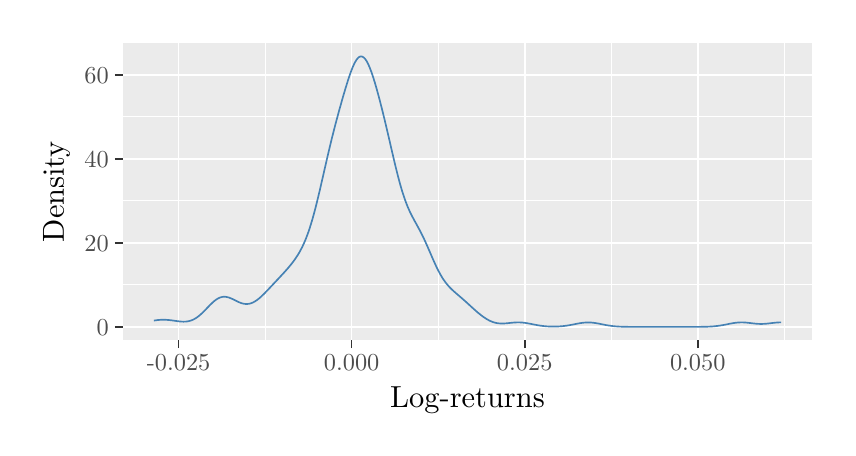
\begin{tikzpicture}[x=1pt,y=1pt]
\definecolor{fillColor}{RGB}{255,255,255}
\path[use as bounding box,fill=fillColor,fill opacity=0.00] (0,0) rectangle (289.08,144.54);
\begin{scope}
\path[clip] (  0.00,  0.00) rectangle (289.08,144.54);
\definecolor{drawColor}{RGB}{255,255,255}
\definecolor{fillColor}{RGB}{255,255,255}

\path[draw=drawColor,line width= 0.6pt,line join=round,line cap=round,fill=fillColor] (  0.00,  0.00) rectangle (289.08,144.54);
\end{scope}
\begin{scope}
\path[clip] ( 34.27, 31.53) rectangle (283.58,139.04);
\definecolor{fillColor}{gray}{0.92}

\path[fill=fillColor] ( 34.27, 31.53) rectangle (283.58,139.04);
\definecolor{drawColor}{RGB}{255,255,255}

\path[draw=drawColor,line width= 0.3pt,line join=round] ( 34.27, 51.60) --
	(283.58, 51.60);

\path[draw=drawColor,line width= 0.3pt,line join=round] ( 34.27, 81.97) --
	(283.58, 81.97);

\path[draw=drawColor,line width= 0.3pt,line join=round] ( 34.27,112.33) --
	(283.58,112.33);

\path[draw=drawColor,line width= 0.3pt,line join=round] ( 85.80, 31.53) --
	( 85.80,139.04);

\path[draw=drawColor,line width= 0.3pt,line join=round] (148.33, 31.53) --
	(148.33,139.04);

\path[draw=drawColor,line width= 0.3pt,line join=round] (210.86, 31.53) --
	(210.86,139.04);

\path[draw=drawColor,line width= 0.3pt,line join=round] (273.40, 31.53) --
	(273.40,139.04);

\path[draw=drawColor,line width= 0.6pt,line join=round] ( 34.27, 36.42) --
	(283.58, 36.42);

\path[draw=drawColor,line width= 0.6pt,line join=round] ( 34.27, 66.78) --
	(283.58, 66.78);

\path[draw=drawColor,line width= 0.6pt,line join=round] ( 34.27, 97.15) --
	(283.58, 97.15);

\path[draw=drawColor,line width= 0.6pt,line join=round] ( 34.27,127.52) --
	(283.58,127.52);

\path[draw=drawColor,line width= 0.6pt,line join=round] ( 54.53, 31.53) --
	( 54.53,139.04);

\path[draw=drawColor,line width= 0.6pt,line join=round] (117.07, 31.53) --
	(117.07,139.04);

\path[draw=drawColor,line width= 0.6pt,line join=round] (179.60, 31.53) --
	(179.60,139.04);

\path[draw=drawColor,line width= 0.6pt,line join=round] (242.13, 31.53) --
	(242.13,139.04);
\definecolor{drawColor}{RGB}{70,130,180}

\path[draw=drawColor,line width= 0.6pt,line join=round] ( 45.60, 38.68) --
	( 46.04, 38.76) --
	( 46.49, 38.82) --
	( 46.93, 38.88) --
	( 47.37, 38.92) --
	( 47.82, 38.96) --
	( 48.26, 38.98) --
	( 48.70, 39.00) --
	( 49.15, 39.00) --
	( 49.59, 38.99) --
	( 50.04, 38.97) --
	( 50.48, 38.94) --
	( 50.92, 38.90) --
	( 51.37, 38.86) --
	( 51.81, 38.81) --
	( 52.25, 38.75) --
	( 52.70, 38.69) --
	( 53.14, 38.62) --
	( 53.58, 38.56) --
	( 54.03, 38.50) --
	( 54.47, 38.44) --
	( 54.91, 38.39) --
	( 55.36, 38.35) --
	( 55.80, 38.32) --
	( 56.25, 38.30) --
	( 56.69, 38.31) --
	( 57.13, 38.33) --
	( 57.58, 38.38) --
	( 58.02, 38.46) --
	( 58.46, 38.56) --
	( 58.91, 38.68) --
	( 59.35, 38.85) --
	( 59.79, 39.04) --
	( 60.24, 39.27) --
	( 60.68, 39.53) --
	( 61.12, 39.82) --
	( 61.57, 40.14) --
	( 62.01, 40.49) --
	( 62.45, 40.87) --
	( 62.90, 41.27) --
	( 63.34, 41.70) --
	( 63.79, 42.14) --
	( 64.23, 42.59) --
	( 64.67, 43.05) --
	( 65.12, 43.52) --
	( 65.56, 43.98) --
	( 66.00, 44.43) --
	( 66.45, 44.86) --
	( 66.89, 45.28) --
	( 67.33, 45.67) --
	( 67.78, 46.03) --
	( 68.22, 46.35) --
	( 68.66, 46.62) --
	( 69.11, 46.85) --
	( 69.55, 47.04) --
	( 69.99, 47.17) --
	( 70.44, 47.27) --
	( 70.88, 47.31) --
	( 71.33, 47.30) --
	( 71.77, 47.25) --
	( 72.21, 47.15) --
	( 72.66, 47.03) --
	( 73.10, 46.87) --
	( 73.54, 46.69) --
	( 73.99, 46.49) --
	( 74.43, 46.27) --
	( 74.87, 46.05) --
	( 75.32, 45.83) --
	( 75.76, 45.61) --
	( 76.20, 45.41) --
	( 76.65, 45.22) --
	( 77.09, 45.05) --
	( 77.53, 44.91) --
	( 77.98, 44.81) --
	( 78.42, 44.73) --
	( 78.87, 44.70) --
	( 79.31, 44.70) --
	( 79.75, 44.73) --
	( 80.20, 44.81) --
	( 80.64, 44.94) --
	( 81.08, 45.10) --
	( 81.53, 45.30) --
	( 81.97, 45.54) --
	( 82.41, 45.81) --
	( 82.86, 46.11) --
	( 83.30, 46.45) --
	( 83.74, 46.81) --
	( 84.19, 47.20) --
	( 84.63, 47.61) --
	( 85.07, 48.04) --
	( 85.52, 48.48) --
	( 85.96, 48.93) --
	( 86.41, 49.39) --
	( 86.85, 49.85) --
	( 87.29, 50.32) --
	( 87.74, 50.80) --
	( 88.18, 51.27) --
	( 88.62, 51.74) --
	( 89.07, 52.22) --
	( 89.51, 52.69) --
	( 89.95, 53.16) --
	( 90.40, 53.63) --
	( 90.84, 54.11) --
	( 91.28, 54.58) --
	( 91.73, 55.06) --
	( 92.17, 55.54) --
	( 92.62, 56.02) --
	( 93.06, 56.51) --
	( 93.50, 57.01) --
	( 93.95, 57.52) --
	( 94.39, 58.04) --
	( 94.83, 58.57) --
	( 95.28, 59.12) --
	( 95.72, 59.68) --
	( 96.16, 60.28) --
	( 96.61, 60.89) --
	( 97.05, 61.54) --
	( 97.49, 62.22) --
	( 97.94, 62.94) --
	( 98.38, 63.71) --
	( 98.82, 64.54) --
	( 99.27, 65.42) --
	( 99.71, 66.36) --
	(100.16, 67.37) --
	(100.60, 68.45) --
	(101.04, 69.61) --
	(101.49, 70.85) --
	(101.93, 72.18) --
	(102.37, 73.59) --
	(102.82, 75.08) --
	(103.26, 76.64) --
	(103.70, 78.28) --
	(104.15, 79.99) --
	(104.59, 81.77) --
	(105.03, 83.60) --
	(105.48, 85.48) --
	(105.92, 87.38) --
	(106.36, 89.32) --
	(106.81, 91.26) --
	(107.25, 93.21) --
	(107.70, 95.15) --
	(108.14, 97.08) --
	(108.58, 98.98) --
	(109.03,100.86) --
	(109.47,102.71) --
	(109.91,104.52) --
	(110.36,106.30) --
	(110.80,108.04) --
	(111.24,109.74) --
	(111.69,111.42) --
	(112.13,113.06) --
	(112.57,114.69) --
	(113.02,116.28) --
	(113.46,117.86) --
	(113.90,119.41) --
	(114.35,120.93) --
	(114.79,122.43) --
	(115.24,123.88) --
	(115.68,125.30) --
	(116.12,126.66) --
	(116.57,127.96) --
	(117.01,129.16) --
	(117.45,130.26) --
	(117.90,131.26) --
	(118.34,132.13) --
	(118.78,132.86) --
	(119.23,133.45) --
	(119.67,133.87) --
	(120.11,134.10) --
	(120.56,134.15) --
	(121.00,134.04) --
	(121.45,133.76) --
	(121.89,133.31) --
	(122.33,132.70) --
	(122.78,131.92) --
	(123.22,130.99) --
	(123.66,129.94) --
	(124.11,128.77) --
	(124.55,127.51) --
	(124.99,126.15) --
	(125.44,124.72) --
	(125.88,123.20) --
	(126.32,121.63) --
	(126.77,120.00) --
	(127.21,118.33) --
	(127.65,116.61) --
	(128.10,114.85) --
	(128.54,113.06) --
	(128.99,111.23) --
	(129.43,109.37) --
	(129.87,107.49) --
	(130.32,105.59) --
	(130.76,103.68) --
	(131.20,101.75) --
	(131.65, 99.83) --
	(132.09, 97.93) --
	(132.53, 96.05) --
	(132.98, 94.21) --
	(133.42, 92.41) --
	(133.86, 90.67) --
	(134.31, 88.99) --
	(134.75, 87.39) --
	(135.19, 85.88) --
	(135.64, 84.45) --
	(136.08, 83.11) --
	(136.53, 81.86) --
	(136.97, 80.69) --
	(137.41, 79.60) --
	(137.86, 78.58) --
	(138.30, 77.64) --
	(138.74, 76.74) --
	(139.19, 75.89) --
	(139.63, 75.06) --
	(140.07, 74.26) --
	(140.52, 73.46) --
	(140.96, 72.65) --
	(141.40, 71.83) --
	(141.85, 70.99) --
	(142.29, 70.13) --
	(142.73, 69.23) --
	(143.18, 68.31) --
	(143.62, 67.36) --
	(144.07, 66.37) --
	(144.51, 65.37) --
	(144.95, 64.35) --
	(145.40, 63.32) --
	(145.84, 62.29) --
	(146.28, 61.27) --
	(146.73, 60.26) --
	(147.17, 59.28) --
	(147.61, 58.32) --
	(148.06, 57.41) --
	(148.50, 56.54) --
	(148.94, 55.70) --
	(149.39, 54.92) --
	(149.83, 54.18) --
	(150.27, 53.50) --
	(150.72, 52.87) --
	(151.16, 52.28) --
	(151.61, 51.72) --
	(152.05, 51.21) --
	(152.49, 50.72) --
	(152.94, 50.27) --
	(153.38, 49.84) --
	(153.82, 49.43) --
	(154.27, 49.03) --
	(154.71, 48.64) --
	(155.15, 48.26) --
	(155.60, 47.88) --
	(156.04, 47.50) --
	(156.48, 47.12) --
	(156.93, 46.73) --
	(157.37, 46.34) --
	(157.82, 45.95) --
	(158.26, 45.56) --
	(158.70, 45.16) --
	(159.15, 44.75) --
	(159.59, 44.35) --
	(160.03, 43.94) --
	(160.48, 43.54) --
	(160.92, 43.13) --
	(161.36, 42.74) --
	(161.81, 42.34) --
	(162.25, 41.95) --
	(162.69, 41.57) --
	(163.14, 41.21) --
	(163.58, 40.85) --
	(164.02, 40.50) --
	(164.47, 40.17) --
	(164.91, 39.86) --
	(165.36, 39.56) --
	(165.80, 39.28) --
	(166.24, 39.03) --
	(166.69, 38.79) --
	(167.13, 38.57) --
	(167.57, 38.38) --
	(168.02, 38.21) --
	(168.46, 38.06) --
	(168.90, 37.94) --
	(169.35, 37.83) --
	(169.79, 37.75) --
	(170.23, 37.70) --
	(170.68, 37.66) --
	(171.12, 37.63) --
	(171.56, 37.63) --
	(172.01, 37.64) --
	(172.45, 37.67) --
	(172.90, 37.70) --
	(173.34, 37.74) --
	(173.78, 37.79) --
	(174.23, 37.84) --
	(174.67, 37.88) --
	(175.11, 37.93) --
	(175.56, 37.97) --
	(176.00, 38.00) --
	(176.44, 38.03) --
	(176.89, 38.04) --
	(177.33, 38.05) --
	(177.77, 38.04) --
	(178.22, 38.02) --
	(178.66, 37.99) --
	(179.10, 37.94) --
	(179.55, 37.89) --
	(179.99, 37.83) --
	(180.44, 37.76) --
	(180.88, 37.68) --
	(181.32, 37.59) --
	(181.77, 37.51) --
	(182.21, 37.42) --
	(182.65, 37.33) --
	(183.10, 37.24) --
	(183.54, 37.16) --
	(183.98, 37.08) --
	(184.43, 37.00) --
	(184.87, 36.93) --
	(185.31, 36.86) --
	(185.76, 36.80) --
	(186.20, 36.74) --
	(186.64, 36.70) --
	(187.09, 36.66) --
	(187.53, 36.62) --
	(187.98, 36.59) --
	(188.42, 36.57) --
	(188.86, 36.55) --
	(189.31, 36.54) --
	(189.75, 36.54) --
	(190.19, 36.54) --
	(190.64, 36.54) --
	(191.08, 36.55) --
	(191.52, 36.57) --
	(191.97, 36.59) --
	(192.41, 36.62) --
	(192.85, 36.65) --
	(193.30, 36.69) --
	(193.74, 36.74) --
	(194.19, 36.79) --
	(194.63, 36.85) --
	(195.07, 36.92) --
	(195.52, 36.99) --
	(195.96, 37.07) --
	(196.40, 37.15) --
	(196.85, 37.23) --
	(197.29, 37.32) --
	(197.73, 37.41) --
	(198.18, 37.50) --
	(198.62, 37.58) --
	(199.06, 37.67) --
	(199.51, 37.74) --
	(199.95, 37.81) --
	(200.39, 37.88) --
	(200.84, 37.93) --
	(201.28, 37.97) --
	(201.73, 38.00) --
	(202.17, 38.02) --
	(202.61, 38.02) --
	(203.06, 38.01) --
	(203.50, 37.99) --
	(203.94, 37.96) --
	(204.39, 37.91) --
	(204.83, 37.85) --
	(205.27, 37.79) --
	(205.72, 37.71) --
	(206.16, 37.63) --
	(206.60, 37.55) --
	(207.05, 37.46) --
	(207.49, 37.37) --
	(207.93, 37.28) --
	(208.38, 37.20) --
	(208.82, 37.11) --
	(209.27, 37.03) --
	(209.71, 36.96) --
	(210.15, 36.89) --
	(210.60, 36.82) --
	(211.04, 36.76) --
	(211.48, 36.71) --
	(211.93, 36.67) --
	(212.37, 36.62) --
	(212.81, 36.59) --
	(213.26, 36.56) --
	(213.70, 36.53) --
	(214.14, 36.51) --
	(214.59, 36.49) --
	(215.03, 36.48) --
	(215.47, 36.46) --
	(215.92, 36.45) --
	(216.36, 36.45) --
	(216.81, 36.44) --
	(217.25, 36.43) --
	(217.69, 36.43) --
	(218.14, 36.43) --
	(218.58, 36.42) --
	(219.02, 36.42) --
	(219.47, 36.42) --
	(219.91, 36.42) --
	(220.35, 36.42) --
	(220.80, 36.42) --
	(221.24, 36.42) --
	(221.68, 36.42) --
	(222.13, 36.42) --
	(222.57, 36.42) --
	(223.02, 36.42) --
	(223.46, 36.42) --
	(223.90, 36.42) --
	(224.35, 36.42) --
	(224.79, 36.42) --
	(225.23, 36.42) --
	(225.68, 36.42) --
	(226.12, 36.42) --
	(226.56, 36.42) --
	(227.01, 36.42) --
	(227.45, 36.42) --
	(227.89, 36.42) --
	(228.34, 36.42) --
	(228.78, 36.42) --
	(229.22, 36.42) --
	(229.67, 36.42) --
	(230.11, 36.42) --
	(230.56, 36.42) --
	(231.00, 36.42) --
	(231.44, 36.42) --
	(231.89, 36.42) --
	(232.33, 36.42) --
	(232.77, 36.42) --
	(233.22, 36.42) --
	(233.66, 36.42) --
	(234.10, 36.42) --
	(234.55, 36.42) --
	(234.99, 36.42) --
	(235.43, 36.42) --
	(235.88, 36.42) --
	(236.32, 36.42) --
	(236.76, 36.42) --
	(237.21, 36.42) --
	(237.65, 36.42) --
	(238.10, 36.42) --
	(238.54, 36.42) --
	(238.98, 36.42) --
	(239.43, 36.42) --
	(239.87, 36.42) --
	(240.31, 36.42) --
	(240.76, 36.42) --
	(241.20, 36.42) --
	(241.64, 36.42) --
	(242.09, 36.43) --
	(242.53, 36.43) --
	(242.97, 36.43) --
	(243.42, 36.44) --
	(243.86, 36.44) --
	(244.30, 36.45) --
	(244.75, 36.46) --
	(245.19, 36.47) --
	(245.64, 36.49) --
	(246.08, 36.51) --
	(246.52, 36.53) --
	(246.97, 36.55) --
	(247.41, 36.58) --
	(247.85, 36.62) --
	(248.30, 36.66) --
	(248.74, 36.71) --
	(249.18, 36.76) --
	(249.63, 36.81) --
	(250.07, 36.88) --
	(250.51, 36.95) --
	(250.96, 37.02) --
	(251.40, 37.10) --
	(251.84, 37.18) --
	(252.29, 37.27) --
	(252.73, 37.36) --
	(253.18, 37.45) --
	(253.62, 37.54) --
	(254.06, 37.62) --
	(254.51, 37.70) --
	(254.95, 37.78) --
	(255.39, 37.85) --
	(255.84, 37.91) --
	(256.28, 37.96) --
	(256.72, 38.00) --
	(257.17, 38.02) --
	(257.61, 38.04) --
	(258.05, 38.04) --
	(258.50, 38.04) --
	(258.94, 38.02) --
	(259.39, 37.99) --
	(259.83, 37.95) --
	(260.27, 37.90) --
	(260.72, 37.85) --
	(261.16, 37.80) --
	(261.60, 37.74) --
	(262.05, 37.69) --
	(262.49, 37.64) --
	(262.93, 37.59) --
	(263.38, 37.55) --
	(263.82, 37.52) --
	(264.26, 37.50) --
	(264.71, 37.48) --
	(265.15, 37.48) --
	(265.59, 37.49) --
	(266.04, 37.51) --
	(266.48, 37.54) --
	(266.93, 37.57) --
	(267.37, 37.62) --
	(267.81, 37.67) --
	(268.26, 37.72) --
	(268.70, 37.78) --
	(269.14, 37.83) --
	(269.59, 37.88) --
	(270.03, 37.93) --
	(270.47, 37.97) --
	(270.92, 38.01) --
	(271.36, 38.03) --
	(271.80, 38.04) --
	(272.25, 38.04);
\end{scope}
\begin{scope}
\path[clip] (  0.00,  0.00) rectangle (289.08,144.54);
\definecolor{drawColor}{gray}{0.30}

\node[text=drawColor,anchor=base east,inner sep=0pt, outer sep=0pt, scale=  0.88] at ( 29.32, 33.39) {0};

\node[text=drawColor,anchor=base east,inner sep=0pt, outer sep=0pt, scale=  0.88] at ( 29.32, 63.75) {20};

\node[text=drawColor,anchor=base east,inner sep=0pt, outer sep=0pt, scale=  0.88] at ( 29.32, 94.12) {40};

\node[text=drawColor,anchor=base east,inner sep=0pt, outer sep=0pt, scale=  0.88] at ( 29.32,124.49) {60};
\end{scope}
\begin{scope}
\path[clip] (  0.00,  0.00) rectangle (289.08,144.54);
\definecolor{drawColor}{gray}{0.20}

\path[draw=drawColor,line width= 0.6pt,line join=round] ( 31.52, 36.42) --
	( 34.27, 36.42);

\path[draw=drawColor,line width= 0.6pt,line join=round] ( 31.52, 66.78) --
	( 34.27, 66.78);

\path[draw=drawColor,line width= 0.6pt,line join=round] ( 31.52, 97.15) --
	( 34.27, 97.15);

\path[draw=drawColor,line width= 0.6pt,line join=round] ( 31.52,127.52) --
	( 34.27,127.52);
\end{scope}
\begin{scope}
\path[clip] (  0.00,  0.00) rectangle (289.08,144.54);
\definecolor{drawColor}{gray}{0.20}

\path[draw=drawColor,line width= 0.6pt,line join=round] ( 54.53, 28.78) --
	( 54.53, 31.53);

\path[draw=drawColor,line width= 0.6pt,line join=round] (117.07, 28.78) --
	(117.07, 31.53);

\path[draw=drawColor,line width= 0.6pt,line join=round] (179.60, 28.78) --
	(179.60, 31.53);

\path[draw=drawColor,line width= 0.6pt,line join=round] (242.13, 28.78) --
	(242.13, 31.53);
\end{scope}
\begin{scope}
\path[clip] (  0.00,  0.00) rectangle (289.08,144.54);
\definecolor{drawColor}{gray}{0.30}

\node[text=drawColor,anchor=base,inner sep=0pt, outer sep=0pt, scale=  0.88] at ( 54.53, 20.52) {-0.025};

\node[text=drawColor,anchor=base,inner sep=0pt, outer sep=0pt, scale=  0.88] at (117.07, 20.52) {0.000};

\node[text=drawColor,anchor=base,inner sep=0pt, outer sep=0pt, scale=  0.88] at (179.60, 20.52) {0.025};

\node[text=drawColor,anchor=base,inner sep=0pt, outer sep=0pt, scale=  0.88] at (242.13, 20.52) {0.050};
\end{scope}
\begin{scope}
\path[clip] (  0.00,  0.00) rectangle (289.08,144.54);
\definecolor{drawColor}{RGB}{0,0,0}

\node[text=drawColor,anchor=base,inner sep=0pt, outer sep=0pt, scale=  1.10] at (158.92,  7.44) {Log-returns};
\end{scope}
\begin{scope}
\path[clip] (  0.00,  0.00) rectangle (289.08,144.54);
\definecolor{drawColor}{RGB}{0,0,0}

\node[text=drawColor,rotate= 90.00,anchor=base,inner sep=0pt, outer sep=0pt, scale=  1.10] at ( 13.08, 85.29) {Density};
\end{scope}
\end{tikzpicture}

  \caption{Historical Apple stock Log-returns distribution}
  \floatfoot{The above densities function is constructed over the historical data of the Apple share of stock price evolution from 18th May 2017 to 18th May 2018.
  
  }
  \label{p:methodology:density:aapl}
\end{figure}


The procedures to calibrate the arguments for MJD and HSV processes are respectively explained at \cref{sub:methodology:calibration:merton,sub:methodology:calibration:heston}.


% SUBSECTION: Merton's model calibration

\subsection{Merton's model calibration}
\label{sub:methodology:calibration:merton}


% SUBSECTION: Heston's model calibration

\subsection{Heston's model calibration}
\label{sub:methodology:calibration:heston}

\subsubsection*{Calibration of parameters for option pricing}

In order to use the function \textit{hsv\_call} based on \cref{eq:other:call:heston} to compute the price of European call options on an underlying with increments driven by the HSV model, the parameters $(V(0), \kappa, \theta, \sigma, \rho)$ must be calibrated with respect to the available option market data.
Consequently, the so estimated parameters will be in line with the risk-neutral measure, or more specifically $\kappa$ and $\theta$, which are the only ones adapted to make \cref{eq:other:hsvvol:riskless} risk-neutral.

To do so, I am going to use the aforementioned least-square non-linear analysis together with data on Apple call option as a template.
In that respect, the theoretical models to calibrate are given by \crefrange{eq:other:call:heston}{eq:other:call:heston:pi2} along with \cref{eq:other:heston:psi}, implemented by the R function \textit{hsv\_call}.

Moreover, to stay in a range of acceptable values, the parameters of the HSV model should lie between some defined boundaries. 

De facto, the mean-reversion speed ($\kappa$), the long-run variance ($\theta$) and the volatility of the volatility ($\sigma$) need to take values that together respect the Feller's condition (see \cref{sub:other:heston:feller}). 
Additionally, $\sigma$ should range between 0 and 1 and, according to \citet{cristo2015} $\kappa$ should be positive to avoid mean aversion.
Although the correlation coefficient $\rho$ may take any value from $[-1, 1]$, typically the correlation between the stock price increments and their intrinsic volatility is negative. Consequently, I set the borders of $\rho$ as being $]0, -1[$.

According to those constraints and due to the presence of multiple local minima, the \textit{lsqnonlin} function returns the \cref{t:methodology:call:heston:estimate1} as the whole sets of parameters that make the function \textit{hsv\_call} better fit with reality.

\begin{table}[ht]
\centering
\begin{tabular}{rrrrr}
  \hline
v0 & theta & sigma & rho & kappa \\ 
  \hline
0.03835 & 0.05144 & 0.30882 & -0.40228 & 1.99821 \\ 
  0.03851 & 0.05142 & 0.29539 & -0.49338 & 1.99931 \\ 
  0.03850 & 0.05241 & 0.30601 & -0.59979 & 1.99843 \\ 
  0.03774 & 0.04832 & 0.30687 & -0.40213 & 3.00036 \\ 
  0.03827 & 0.04954 & 0.40690 & -0.40189 & 3.00011 \\ 
  0.03883 & 0.04798 & 0.30747 & -0.50211 & 3.00015 \\ 
  0.03910 & 0.04948 & 0.40736 & -0.50193 & 3.00005 \\ 
  0.03695 & 0.04703 & 0.30697 & -0.40288 & 4.00092 \\ 
  0.04449 & 0.04443 & 0.40682 & -0.40289 & 4.00079 \\ 
  0.03798 & 0.04872 & 0.50379 & -0.39878 & 4.00106 \\ 
  0.04091 & 0.04651 & 0.40705 & -0.50227 & 4.00097 \\ 
  0.03740 & 0.04754 & 0.30583 & -0.60126 & 4.00096 \\ 
  0.03890 & 0.04792 & 0.40565 & -0.60086 & 4.00091 \\ 
  0.03661 & 0.04604 & 0.30659 & -0.40295 & 5.00152 \\ 
  0.04034 & 0.04547 & 0.40591 & -0.40298 & 5.00153 \\ 
  0.04111 & 0.04558 & 0.50652 & -0.40298 & 5.00144 \\ 
  0.04034 & 0.04720 & 0.60647 & -0.40250 & 5.00138 \\ 
  0.03921 & 0.04709 & 0.50753 & -0.50170 & 5.00152 \\ 
  0.03789 & 0.04656 & 0.30488 & -0.80072 & 5.00164 \\ 
   \hline
\end{tabular}
\caption{Best estimates for HSV call option model} 
\label{t:methodology:call:heston:estimate1}
\end{table}

Otherwise, The set \ref{eq:methodology:arg:heston:riskneutral} is the one making respond the model the best with what is observed in reality.
Indeed when passing that set to the R function \textit{call\_heston}, for all strikes of \cref{t:methodology:strike} and maturities of \cref{t:methodology:maturity}, more than $70\%$ of the so generated prices are within the bid-ask spread of the Apple option historical data.

\begin{align}
  \left \{
  \begin{array}{lcl}
    V(0) &= &0.03798218, \\
    \theta &= &0.04871543, \\
    \sigma &= &0.50378803, \\
    \rho &= &-0.39877827, \\
    \kappa &= &4.00105546 
  \end{array}
  \right \}  
  \label{eq:methodology:arg:heston:riskneutral}
\end{align}

\cref{{p:methodology:impliedvol:aapl:heston}} confronts the blue colored volatility smiles computed from market data, with those dotted in red, calculated from the function \textit{hsv\_call}, which takes the items of the set \ref{eq:methodology:arg:heston:riskneutral} as parameters.

\begin{figure}[H]
  \centering
  % Created by tikzDevice version 0.11 on 2018-07-18 22:48:11
% !TEX encoding = UTF-8 Unicode
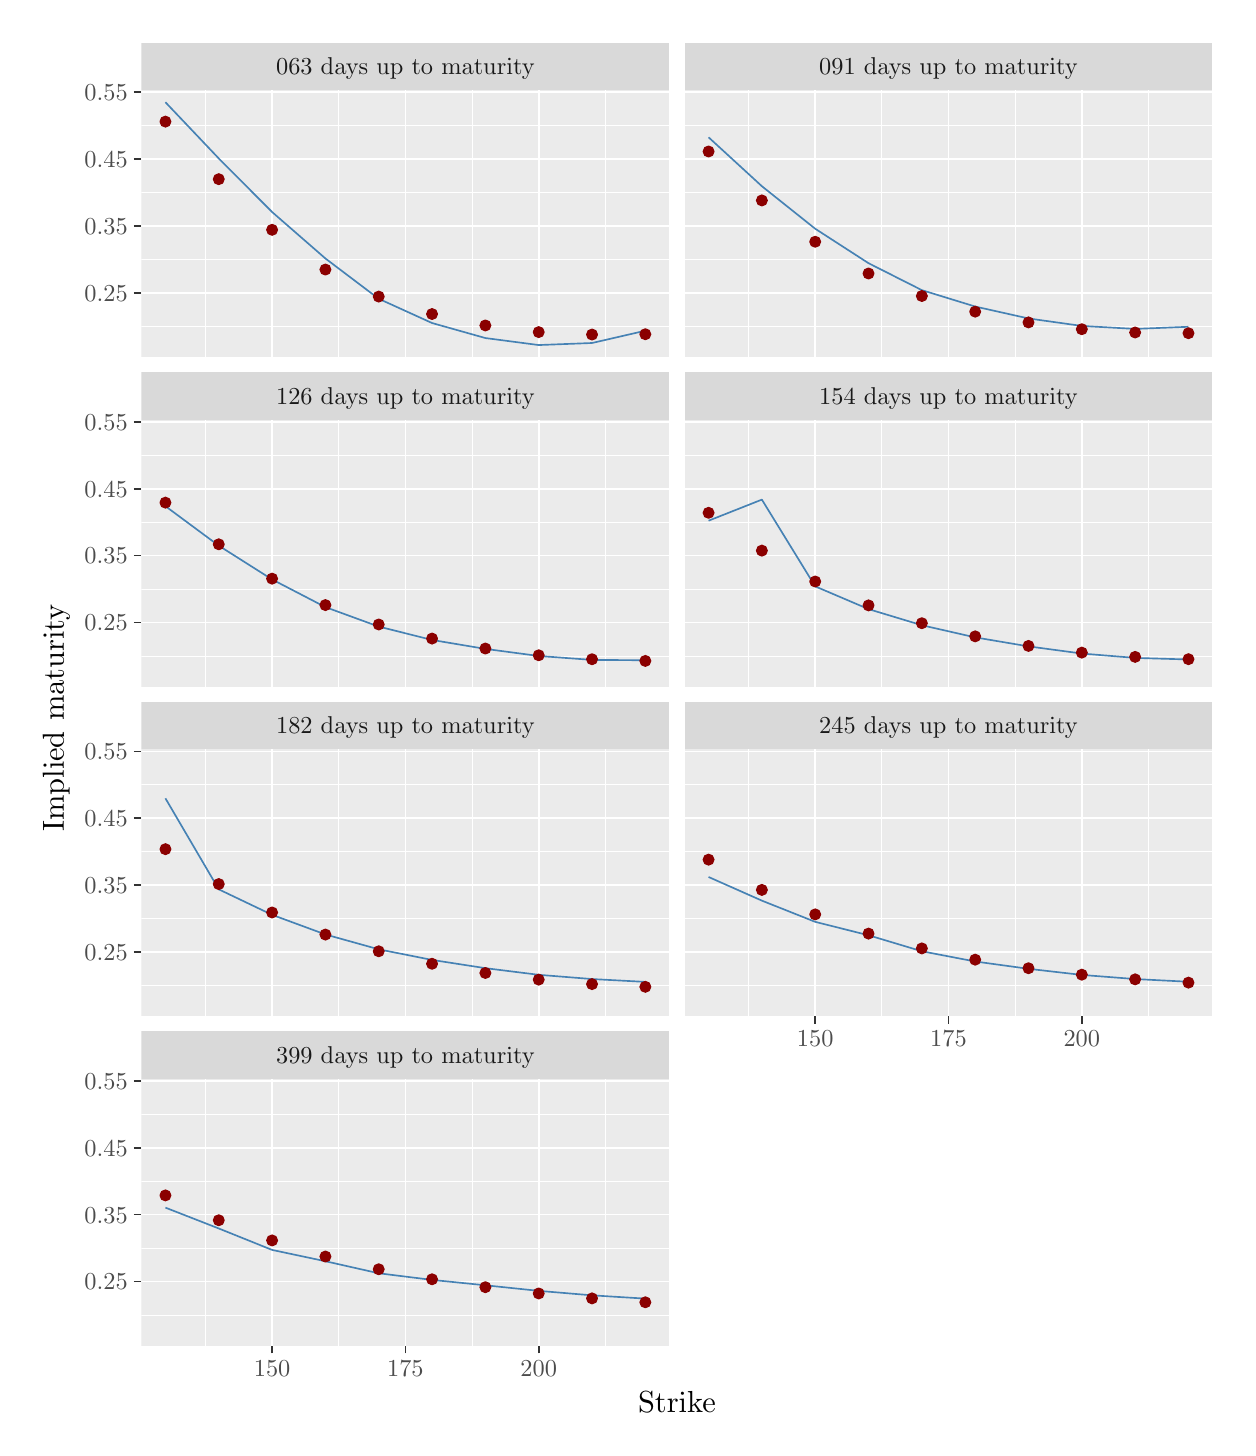
\begin{tikzpicture}[x=1pt,y=1pt]
\definecolor{fillColor}{RGB}{255,255,255}
\path[use as bounding box,fill=fillColor,fill opacity=0.00] (0,0) rectangle (433.62,505.89);
\begin{scope}
\path[clip] (  0.00,  0.00) rectangle (433.62,505.89);
\definecolor{drawColor}{RGB}{255,255,255}
\definecolor{fillColor}{RGB}{255,255,255}

\path[draw=drawColor,line width= 0.6pt,line join=round,line cap=round,fill=fillColor] (  0.00,  0.00) rectangle (433.62,505.89);
\end{scope}
\begin{scope}
\path[clip] ( 41.11,386.81) rectangle (231.87,483.33);
\definecolor{fillColor}{gray}{0.92}

\path[fill=fillColor] ( 41.11,386.81) rectangle (231.87,483.33);
\definecolor{drawColor}{RGB}{255,255,255}

\path[draw=drawColor,line width= 0.3pt,line join=round] ( 41.11,397.93) --
	(231.87,397.93);

\path[draw=drawColor,line width= 0.3pt,line join=round] ( 41.11,422.11) --
	(231.87,422.11);

\path[draw=drawColor,line width= 0.3pt,line join=round] ( 41.11,446.28) --
	(231.87,446.28);

\path[draw=drawColor,line width= 0.3pt,line join=round] ( 41.11,470.45) --
	(231.87,470.45);

\path[draw=drawColor,line width= 0.3pt,line join=round] ( 64.23,386.81) --
	( 64.23,483.33);

\path[draw=drawColor,line width= 0.3pt,line join=round] (112.40,386.81) --
	(112.40,483.33);

\path[draw=drawColor,line width= 0.3pt,line join=round] (160.57,386.81) --
	(160.57,483.33);

\path[draw=drawColor,line width= 0.3pt,line join=round] (208.74,386.81) --
	(208.74,483.33);

\path[draw=drawColor,line width= 0.6pt,line join=round] ( 41.11,410.02) --
	(231.87,410.02);

\path[draw=drawColor,line width= 0.6pt,line join=round] ( 41.11,434.19) --
	(231.87,434.19);

\path[draw=drawColor,line width= 0.6pt,line join=round] ( 41.11,458.37) --
	(231.87,458.37);

\path[draw=drawColor,line width= 0.6pt,line join=round] ( 41.11,482.54) --
	(231.87,482.54);

\path[draw=drawColor,line width= 0.6pt,line join=round] ( 88.32,386.81) --
	( 88.32,483.33);

\path[draw=drawColor,line width= 0.6pt,line join=round] (136.49,386.81) --
	(136.49,483.33);

\path[draw=drawColor,line width= 0.6pt,line join=round] (184.66,386.81) --
	(184.66,483.33);
\definecolor{drawColor}{RGB}{70,130,180}

\path[draw=drawColor,line width= 0.6pt,line join=round] ( 49.78,478.94) --
	( 69.05,458.63) --
	( 88.32,439.27) --
	(107.59,422.48) --
	(126.85,407.92) --
	(146.12,399.16) --
	(165.39,393.73) --
	(184.66,391.20) --
	(203.93,391.94) --
	(223.19,396.38);
\definecolor{drawColor}{RGB}{139,0,0}
\definecolor{fillColor}{RGB}{139,0,0}

\path[draw=drawColor,line width= 0.4pt,line join=round,line cap=round,fill=fillColor] ( 49.78,471.94) circle (  1.96);

\path[draw=drawColor,line width= 0.4pt,line join=round,line cap=round,fill=fillColor] ( 69.05,451.14) circle (  1.96);

\path[draw=drawColor,line width= 0.4pt,line join=round,line cap=round,fill=fillColor] ( 88.32,432.84) circle (  1.96);

\path[draw=drawColor,line width= 0.4pt,line join=round,line cap=round,fill=fillColor] (107.59,418.48) circle (  1.96);

\path[draw=drawColor,line width= 0.4pt,line join=round,line cap=round,fill=fillColor] (126.85,408.72) circle (  1.96);

\path[draw=drawColor,line width= 0.4pt,line join=round,line cap=round,fill=fillColor] (146.12,402.41) circle (  1.96);

\path[draw=drawColor,line width= 0.4pt,line join=round,line cap=round,fill=fillColor] (165.39,398.28) circle (  1.96);

\path[draw=drawColor,line width= 0.4pt,line join=round,line cap=round,fill=fillColor] (184.66,395.88) circle (  1.96);

\path[draw=drawColor,line width= 0.4pt,line join=round,line cap=round,fill=fillColor] (203.93,394.99) circle (  1.96);

\path[draw=drawColor,line width= 0.4pt,line join=round,line cap=round,fill=fillColor] (223.19,395.11) circle (  1.96);
\end{scope}
\begin{scope}
\path[clip] ( 41.11,267.74) rectangle (231.87,364.25);
\definecolor{fillColor}{gray}{0.92}

\path[fill=fillColor] ( 41.11,267.74) rectangle (231.87,364.25);
\definecolor{drawColor}{RGB}{255,255,255}

\path[draw=drawColor,line width= 0.3pt,line join=round] ( 41.11,278.86) --
	(231.87,278.86);

\path[draw=drawColor,line width= 0.3pt,line join=round] ( 41.11,303.03) --
	(231.87,303.03);

\path[draw=drawColor,line width= 0.3pt,line join=round] ( 41.11,327.20) --
	(231.87,327.20);

\path[draw=drawColor,line width= 0.3pt,line join=round] ( 41.11,351.38) --
	(231.87,351.38);

\path[draw=drawColor,line width= 0.3pt,line join=round] ( 64.23,267.74) --
	( 64.23,364.25);

\path[draw=drawColor,line width= 0.3pt,line join=round] (112.40,267.74) --
	(112.40,364.25);

\path[draw=drawColor,line width= 0.3pt,line join=round] (160.57,267.74) --
	(160.57,364.25);

\path[draw=drawColor,line width= 0.3pt,line join=round] (208.74,267.74) --
	(208.74,364.25);

\path[draw=drawColor,line width= 0.6pt,line join=round] ( 41.11,290.95) --
	(231.87,290.95);

\path[draw=drawColor,line width= 0.6pt,line join=round] ( 41.11,315.12) --
	(231.87,315.12);

\path[draw=drawColor,line width= 0.6pt,line join=round] ( 41.11,339.29) --
	(231.87,339.29);

\path[draw=drawColor,line width= 0.6pt,line join=round] ( 41.11,363.46) --
	(231.87,363.46);

\path[draw=drawColor,line width= 0.6pt,line join=round] ( 88.32,267.74) --
	( 88.32,364.25);

\path[draw=drawColor,line width= 0.6pt,line join=round] (136.49,267.74) --
	(136.49,364.25);

\path[draw=drawColor,line width= 0.6pt,line join=round] (184.66,267.74) --
	(184.66,364.25);
\definecolor{drawColor}{RGB}{70,130,180}

\path[draw=drawColor,line width= 0.6pt,line join=round] ( 49.78,332.98) --
	( 69.05,318.71) --
	( 88.32,306.50) --
	(107.59,296.51) --
	(126.85,289.47) --
	(146.12,284.64) --
	(165.39,281.41) --
	(184.66,278.85) --
	(203.93,277.43) --
	(223.19,277.30);
\definecolor{drawColor}{RGB}{139,0,0}
\definecolor{fillColor}{RGB}{139,0,0}

\path[draw=drawColor,line width= 0.4pt,line join=round,line cap=round,fill=fillColor] ( 49.78,334.26) circle (  1.96);

\path[draw=drawColor,line width= 0.4pt,line join=round,line cap=round,fill=fillColor] ( 69.05,319.20) circle (  1.96);

\path[draw=drawColor,line width= 0.4pt,line join=round,line cap=round,fill=fillColor] ( 88.32,306.79) circle (  1.96);

\path[draw=drawColor,line width= 0.4pt,line join=round,line cap=round,fill=fillColor] (107.59,297.24) circle (  1.96);

\path[draw=drawColor,line width= 0.4pt,line join=round,line cap=round,fill=fillColor] (126.85,290.23) circle (  1.96);

\path[draw=drawColor,line width= 0.4pt,line join=round,line cap=round,fill=fillColor] (146.12,285.14) circle (  1.96);

\path[draw=drawColor,line width= 0.4pt,line join=round,line cap=round,fill=fillColor] (165.39,281.54) circle (  1.96);

\path[draw=drawColor,line width= 0.4pt,line join=round,line cap=round,fill=fillColor] (184.66,279.10) circle (  1.96);

\path[draw=drawColor,line width= 0.4pt,line join=round,line cap=round,fill=fillColor] (203.93,277.67) circle (  1.96);

\path[draw=drawColor,line width= 0.4pt,line join=round,line cap=round,fill=fillColor] (223.19,277.06) circle (  1.96);
\end{scope}
\begin{scope}
\path[clip] ( 41.11,148.66) rectangle (231.87,245.18);
\definecolor{fillColor}{gray}{0.92}

\path[fill=fillColor] ( 41.11,148.66) rectangle (231.87,245.18);
\definecolor{drawColor}{RGB}{255,255,255}

\path[draw=drawColor,line width= 0.3pt,line join=round] ( 41.11,159.78) --
	(231.87,159.78);

\path[draw=drawColor,line width= 0.3pt,line join=round] ( 41.11,183.96) --
	(231.87,183.96);

\path[draw=drawColor,line width= 0.3pt,line join=round] ( 41.11,208.13) --
	(231.87,208.13);

\path[draw=drawColor,line width= 0.3pt,line join=round] ( 41.11,232.30) --
	(231.87,232.30);

\path[draw=drawColor,line width= 0.3pt,line join=round] ( 64.23,148.66) --
	( 64.23,245.18);

\path[draw=drawColor,line width= 0.3pt,line join=round] (112.40,148.66) --
	(112.40,245.18);

\path[draw=drawColor,line width= 0.3pt,line join=round] (160.57,148.66) --
	(160.57,245.18);

\path[draw=drawColor,line width= 0.3pt,line join=round] (208.74,148.66) --
	(208.74,245.18);

\path[draw=drawColor,line width= 0.6pt,line join=round] ( 41.11,171.87) --
	(231.87,171.87);

\path[draw=drawColor,line width= 0.6pt,line join=round] ( 41.11,196.04) --
	(231.87,196.04);

\path[draw=drawColor,line width= 0.6pt,line join=round] ( 41.11,220.21) --
	(231.87,220.21);

\path[draw=drawColor,line width= 0.6pt,line join=round] ( 41.11,244.39) --
	(231.87,244.39);

\path[draw=drawColor,line width= 0.6pt,line join=round] ( 88.32,148.66) --
	( 88.32,245.18);

\path[draw=drawColor,line width= 0.6pt,line join=round] (136.49,148.66) --
	(136.49,245.18);

\path[draw=drawColor,line width= 0.6pt,line join=round] (184.66,148.66) --
	(184.66,245.18);
\definecolor{drawColor}{RGB}{70,130,180}

\path[draw=drawColor,line width= 0.6pt,line join=round] ( 49.78,227.41) --
	( 69.05,194.52) --
	( 88.32,185.32) --
	(107.59,178.22) --
	(126.85,172.85) --
	(146.12,169.02) --
	(165.39,166.04) --
	(184.66,163.64) --
	(203.93,162.11) --
	(223.19,161.08);
\definecolor{drawColor}{RGB}{139,0,0}
\definecolor{fillColor}{RGB}{139,0,0}

\path[draw=drawColor,line width= 0.4pt,line join=round,line cap=round,fill=fillColor] ( 49.78,209.04) circle (  1.96);

\path[draw=drawColor,line width= 0.4pt,line join=round,line cap=round,fill=fillColor] ( 69.05,196.43) circle (  1.96);

\path[draw=drawColor,line width= 0.4pt,line join=round,line cap=round,fill=fillColor] ( 88.32,186.16) circle (  1.96);

\path[draw=drawColor,line width= 0.4pt,line join=round,line cap=round,fill=fillColor] (107.59,178.18) circle (  1.96);

\path[draw=drawColor,line width= 0.4pt,line join=round,line cap=round,fill=fillColor] (126.85,172.14) circle (  1.96);

\path[draw=drawColor,line width= 0.4pt,line join=round,line cap=round,fill=fillColor] (146.12,167.63) circle (  1.96);

\path[draw=drawColor,line width= 0.4pt,line join=round,line cap=round,fill=fillColor] (165.39,164.30) circle (  1.96);

\path[draw=drawColor,line width= 0.4pt,line join=round,line cap=round,fill=fillColor] (184.66,161.90) circle (  1.96);

\path[draw=drawColor,line width= 0.4pt,line join=round,line cap=round,fill=fillColor] (203.93,160.28) circle (  1.96);

\path[draw=drawColor,line width= 0.4pt,line join=round,line cap=round,fill=fillColor] (223.19,159.30) circle (  1.96);
\end{scope}
\begin{scope}
\path[clip] ( 41.11, 29.59) rectangle (231.87,126.10);
\definecolor{fillColor}{gray}{0.92}

\path[fill=fillColor] ( 41.11, 29.59) rectangle (231.87,126.10);
\definecolor{drawColor}{RGB}{255,255,255}

\path[draw=drawColor,line width= 0.3pt,line join=round] ( 41.11, 40.71) --
	(231.87, 40.71);

\path[draw=drawColor,line width= 0.3pt,line join=round] ( 41.11, 64.88) --
	(231.87, 64.88);

\path[draw=drawColor,line width= 0.3pt,line join=round] ( 41.11, 89.05) --
	(231.87, 89.05);

\path[draw=drawColor,line width= 0.3pt,line join=round] ( 41.11,113.22) --
	(231.87,113.22);

\path[draw=drawColor,line width= 0.3pt,line join=round] ( 64.23, 29.59) --
	( 64.23,126.10);

\path[draw=drawColor,line width= 0.3pt,line join=round] (112.40, 29.59) --
	(112.40,126.10);

\path[draw=drawColor,line width= 0.3pt,line join=round] (160.57, 29.59) --
	(160.57,126.10);

\path[draw=drawColor,line width= 0.3pt,line join=round] (208.74, 29.59) --
	(208.74,126.10);

\path[draw=drawColor,line width= 0.6pt,line join=round] ( 41.11, 52.79) --
	(231.87, 52.79);

\path[draw=drawColor,line width= 0.6pt,line join=round] ( 41.11, 76.97) --
	(231.87, 76.97);

\path[draw=drawColor,line width= 0.6pt,line join=round] ( 41.11,101.14) --
	(231.87,101.14);

\path[draw=drawColor,line width= 0.6pt,line join=round] ( 41.11,125.31) --
	(231.87,125.31);

\path[draw=drawColor,line width= 0.6pt,line join=round] ( 88.32, 29.59) --
	( 88.32,126.10);

\path[draw=drawColor,line width= 0.6pt,line join=round] (136.49, 29.59) --
	(136.49,126.10);

\path[draw=drawColor,line width= 0.6pt,line join=round] (184.66, 29.59) --
	(184.66,126.10);
\definecolor{drawColor}{RGB}{70,130,180}

\path[draw=drawColor,line width= 0.6pt,line join=round] ( 49.78, 79.51) --
	( 69.05, 71.98) --
	( 88.32, 64.23) --
	(107.59, 60.14) --
	(126.85, 55.79) --
	(146.12, 53.40) --
	(165.39, 51.45) --
	(184.66, 49.44) --
	(203.93, 47.82) --
	(223.19, 46.63);
\definecolor{drawColor}{RGB}{139,0,0}
\definecolor{fillColor}{RGB}{139,0,0}

\path[draw=drawColor,line width= 0.4pt,line join=round,line cap=round,fill=fillColor] ( 49.78, 83.93) circle (  1.96);

\path[draw=drawColor,line width= 0.4pt,line join=round,line cap=round,fill=fillColor] ( 69.05, 74.95) circle (  1.96);

\path[draw=drawColor,line width= 0.4pt,line join=round,line cap=round,fill=fillColor] ( 88.32, 67.66) circle (  1.96);

\path[draw=drawColor,line width= 0.4pt,line join=round,line cap=round,fill=fillColor] (107.59, 61.84) circle (  1.96);

\path[draw=drawColor,line width= 0.4pt,line join=round,line cap=round,fill=fillColor] (126.85, 57.24) circle (  1.96);

\path[draw=drawColor,line width= 0.4pt,line join=round,line cap=round,fill=fillColor] (146.12, 53.62) circle (  1.96);

\path[draw=drawColor,line width= 0.4pt,line join=round,line cap=round,fill=fillColor] (165.39, 50.76) circle (  1.96);

\path[draw=drawColor,line width= 0.4pt,line join=round,line cap=round,fill=fillColor] (184.66, 48.50) circle (  1.96);

\path[draw=drawColor,line width= 0.4pt,line join=round,line cap=round,fill=fillColor] (203.93, 46.72) circle (  1.96);

\path[draw=drawColor,line width= 0.4pt,line join=round,line cap=round,fill=fillColor] (223.19, 45.31) circle (  1.96);
\end{scope}
\begin{scope}
\path[clip] (237.37,386.81) rectangle (428.12,483.33);
\definecolor{fillColor}{gray}{0.92}

\path[fill=fillColor] (237.37,386.81) rectangle (428.12,483.33);
\definecolor{drawColor}{RGB}{255,255,255}

\path[draw=drawColor,line width= 0.3pt,line join=round] (237.37,397.93) --
	(428.12,397.93);

\path[draw=drawColor,line width= 0.3pt,line join=round] (237.37,422.11) --
	(428.12,422.11);

\path[draw=drawColor,line width= 0.3pt,line join=round] (237.37,446.28) --
	(428.12,446.28);

\path[draw=drawColor,line width= 0.3pt,line join=round] (237.37,470.45) --
	(428.12,470.45);

\path[draw=drawColor,line width= 0.3pt,line join=round] (260.49,386.81) --
	(260.49,483.33);

\path[draw=drawColor,line width= 0.3pt,line join=round] (308.66,386.81) --
	(308.66,483.33);

\path[draw=drawColor,line width= 0.3pt,line join=round] (356.83,386.81) --
	(356.83,483.33);

\path[draw=drawColor,line width= 0.3pt,line join=round] (405.00,386.81) --
	(405.00,483.33);

\path[draw=drawColor,line width= 0.6pt,line join=round] (237.37,410.02) --
	(428.12,410.02);

\path[draw=drawColor,line width= 0.6pt,line join=round] (237.37,434.19) --
	(428.12,434.19);

\path[draw=drawColor,line width= 0.6pt,line join=round] (237.37,458.37) --
	(428.12,458.37);

\path[draw=drawColor,line width= 0.6pt,line join=round] (237.37,482.54) --
	(428.12,482.54);

\path[draw=drawColor,line width= 0.6pt,line join=round] (284.57,386.81) --
	(284.57,483.33);

\path[draw=drawColor,line width= 0.6pt,line join=round] (332.74,386.81) --
	(332.74,483.33);

\path[draw=drawColor,line width= 0.6pt,line join=round] (380.91,386.81) --
	(380.91,483.33);
\definecolor{drawColor}{RGB}{70,130,180}

\path[draw=drawColor,line width= 0.6pt,line join=round] (246.04,466.27) --
	(265.30,448.60) --
	(284.57,433.23) --
	(303.84,420.78) --
	(323.11,411.04) --
	(342.38,405.12) --
	(361.64,400.81) --
	(380.91,398.11) --
	(400.18,397.03) --
	(419.45,397.80);
\definecolor{drawColor}{RGB}{139,0,0}
\definecolor{fillColor}{RGB}{139,0,0}

\path[draw=drawColor,line width= 0.4pt,line join=round,line cap=round,fill=fillColor] (246.04,461.14) circle (  1.96);

\path[draw=drawColor,line width= 0.4pt,line join=round,line cap=round,fill=fillColor] (265.30,443.46) circle (  1.96);

\path[draw=drawColor,line width= 0.4pt,line join=round,line cap=round,fill=fillColor] (284.57,428.53) circle (  1.96);

\path[draw=drawColor,line width= 0.4pt,line join=round,line cap=round,fill=fillColor] (303.84,417.06) circle (  1.96);

\path[draw=drawColor,line width= 0.4pt,line join=round,line cap=round,fill=fillColor] (323.11,408.92) circle (  1.96);

\path[draw=drawColor,line width= 0.4pt,line join=round,line cap=round,fill=fillColor] (342.38,403.27) circle (  1.96);

\path[draw=drawColor,line width= 0.4pt,line join=round,line cap=round,fill=fillColor] (361.64,399.38) circle (  1.96);

\path[draw=drawColor,line width= 0.4pt,line join=round,line cap=round,fill=fillColor] (380.91,396.93) circle (  1.96);

\path[draw=drawColor,line width= 0.4pt,line join=round,line cap=round,fill=fillColor] (400.18,395.74) circle (  1.96);

\path[draw=drawColor,line width= 0.4pt,line join=round,line cap=round,fill=fillColor] (419.45,395.48) circle (  1.96);
\end{scope}
\begin{scope}
\path[clip] (237.37,267.74) rectangle (428.12,364.25);
\definecolor{fillColor}{gray}{0.92}

\path[fill=fillColor] (237.37,267.74) rectangle (428.12,364.25);
\definecolor{drawColor}{RGB}{255,255,255}

\path[draw=drawColor,line width= 0.3pt,line join=round] (237.37,278.86) --
	(428.12,278.86);

\path[draw=drawColor,line width= 0.3pt,line join=round] (237.37,303.03) --
	(428.12,303.03);

\path[draw=drawColor,line width= 0.3pt,line join=round] (237.37,327.20) --
	(428.12,327.20);

\path[draw=drawColor,line width= 0.3pt,line join=round] (237.37,351.38) --
	(428.12,351.38);

\path[draw=drawColor,line width= 0.3pt,line join=round] (260.49,267.74) --
	(260.49,364.25);

\path[draw=drawColor,line width= 0.3pt,line join=round] (308.66,267.74) --
	(308.66,364.25);

\path[draw=drawColor,line width= 0.3pt,line join=round] (356.83,267.74) --
	(356.83,364.25);

\path[draw=drawColor,line width= 0.3pt,line join=round] (405.00,267.74) --
	(405.00,364.25);

\path[draw=drawColor,line width= 0.6pt,line join=round] (237.37,290.95) --
	(428.12,290.95);

\path[draw=drawColor,line width= 0.6pt,line join=round] (237.37,315.12) --
	(428.12,315.12);

\path[draw=drawColor,line width= 0.6pt,line join=round] (237.37,339.29) --
	(428.12,339.29);

\path[draw=drawColor,line width= 0.6pt,line join=round] (237.37,363.46) --
	(428.12,363.46);

\path[draw=drawColor,line width= 0.6pt,line join=round] (284.57,267.74) --
	(284.57,364.25);

\path[draw=drawColor,line width= 0.6pt,line join=round] (332.74,267.74) --
	(332.74,364.25);

\path[draw=drawColor,line width= 0.6pt,line join=round] (380.91,267.74) --
	(380.91,364.25);
\definecolor{drawColor}{RGB}{70,130,180}

\path[draw=drawColor,line width= 0.6pt,line join=round] (246.04,327.73) --
	(265.30,335.35) --
	(284.57,304.00) --
	(303.84,295.78) --
	(323.11,289.96) --
	(342.38,285.57) --
	(361.64,282.32) --
	(380.91,279.73) --
	(400.18,278.15) --
	(419.45,277.58);
\definecolor{drawColor}{RGB}{139,0,0}
\definecolor{fillColor}{RGB}{139,0,0}

\path[draw=drawColor,line width= 0.4pt,line join=round,line cap=round,fill=fillColor] (246.04,330.58) circle (  1.96);

\path[draw=drawColor,line width= 0.4pt,line join=round,line cap=round,fill=fillColor] (265.30,316.92) circle (  1.96);

\path[draw=drawColor,line width= 0.4pt,line join=round,line cap=round,fill=fillColor] (284.57,305.76) circle (  1.96);

\path[draw=drawColor,line width= 0.4pt,line join=round,line cap=round,fill=fillColor] (303.84,297.13) circle (  1.96);

\path[draw=drawColor,line width= 0.4pt,line join=round,line cap=round,fill=fillColor] (323.11,290.69) circle (  1.96);

\path[draw=drawColor,line width= 0.4pt,line join=round,line cap=round,fill=fillColor] (342.38,285.94) circle (  1.96);

\path[draw=drawColor,line width= 0.4pt,line join=round,line cap=round,fill=fillColor] (361.64,282.48) circle (  1.96);

\path[draw=drawColor,line width= 0.4pt,line join=round,line cap=round,fill=fillColor] (380.91,280.06) circle (  1.96);

\path[draw=drawColor,line width= 0.4pt,line join=round,line cap=round,fill=fillColor] (400.18,278.52) circle (  1.96);

\path[draw=drawColor,line width= 0.4pt,line join=round,line cap=round,fill=fillColor] (419.45,277.69) circle (  1.96);
\end{scope}
\begin{scope}
\path[clip] (237.37,148.66) rectangle (428.12,245.18);
\definecolor{fillColor}{gray}{0.92}

\path[fill=fillColor] (237.37,148.66) rectangle (428.12,245.18);
\definecolor{drawColor}{RGB}{255,255,255}

\path[draw=drawColor,line width= 0.3pt,line join=round] (237.37,159.78) --
	(428.12,159.78);

\path[draw=drawColor,line width= 0.3pt,line join=round] (237.37,183.96) --
	(428.12,183.96);

\path[draw=drawColor,line width= 0.3pt,line join=round] (237.37,208.13) --
	(428.12,208.13);

\path[draw=drawColor,line width= 0.3pt,line join=round] (237.37,232.30) --
	(428.12,232.30);

\path[draw=drawColor,line width= 0.3pt,line join=round] (260.49,148.66) --
	(260.49,245.18);

\path[draw=drawColor,line width= 0.3pt,line join=round] (308.66,148.66) --
	(308.66,245.18);

\path[draw=drawColor,line width= 0.3pt,line join=round] (356.83,148.66) --
	(356.83,245.18);

\path[draw=drawColor,line width= 0.3pt,line join=round] (405.00,148.66) --
	(405.00,245.18);

\path[draw=drawColor,line width= 0.6pt,line join=round] (237.37,171.87) --
	(428.12,171.87);

\path[draw=drawColor,line width= 0.6pt,line join=round] (237.37,196.04) --
	(428.12,196.04);

\path[draw=drawColor,line width= 0.6pt,line join=round] (237.37,220.21) --
	(428.12,220.21);

\path[draw=drawColor,line width= 0.6pt,line join=round] (237.37,244.39) --
	(428.12,244.39);

\path[draw=drawColor,line width= 0.6pt,line join=round] (284.57,148.66) --
	(284.57,245.18);

\path[draw=drawColor,line width= 0.6pt,line join=round] (332.74,148.66) --
	(332.74,245.18);

\path[draw=drawColor,line width= 0.6pt,line join=round] (380.91,148.66) --
	(380.91,245.18);
\definecolor{drawColor}{RGB}{70,130,180}

\path[draw=drawColor,line width= 0.6pt,line join=round] (246.04,198.99) --
	(265.30,190.44) --
	(284.57,182.78) --
	(303.84,177.93) --
	(323.11,172.15) --
	(342.38,168.45) --
	(361.64,165.81) --
	(380.91,163.60) --
	(400.18,162.11) --
	(419.45,161.13);
\definecolor{drawColor}{RGB}{139,0,0}
\definecolor{fillColor}{RGB}{139,0,0}

\path[draw=drawColor,line width= 0.4pt,line join=round,line cap=round,fill=fillColor] (246.04,205.25) circle (  1.96);

\path[draw=drawColor,line width= 0.4pt,line join=round,line cap=round,fill=fillColor] (265.30,194.32) circle (  1.96);

\path[draw=drawColor,line width= 0.4pt,line join=round,line cap=round,fill=fillColor] (284.57,185.47) circle (  1.96);

\path[draw=drawColor,line width= 0.4pt,line join=round,line cap=round,fill=fillColor] (303.84,178.53) circle (  1.96);

\path[draw=drawColor,line width= 0.4pt,line join=round,line cap=round,fill=fillColor] (323.11,173.18) circle (  1.96);

\path[draw=drawColor,line width= 0.4pt,line join=round,line cap=round,fill=fillColor] (342.38,169.11) circle (  1.96);

\path[draw=drawColor,line width= 0.4pt,line join=round,line cap=round,fill=fillColor] (361.64,166.02) circle (  1.96);

\path[draw=drawColor,line width= 0.4pt,line join=round,line cap=round,fill=fillColor] (380.91,163.69) circle (  1.96);

\path[draw=drawColor,line width= 0.4pt,line join=round,line cap=round,fill=fillColor] (400.18,162.00) circle (  1.96);

\path[draw=drawColor,line width= 0.4pt,line join=round,line cap=round,fill=fillColor] (419.45,160.81) circle (  1.96);
\end{scope}
\begin{scope}
\path[clip] ( 41.11,126.10) rectangle (231.87,143.16);
\definecolor{fillColor}{gray}{0.85}

\path[fill=fillColor] ( 41.11,126.10) rectangle (231.87,143.16);
\definecolor{drawColor}{gray}{0.10}

\node[text=drawColor,anchor=base,inner sep=0pt, outer sep=0pt, scale=  0.88] at (136.49,131.60) {399 days up to maturity};
\end{scope}
\begin{scope}
\path[clip] ( 41.11,245.18) rectangle (231.87,262.24);
\definecolor{fillColor}{gray}{0.85}

\path[fill=fillColor] ( 41.11,245.18) rectangle (231.87,262.24);
\definecolor{drawColor}{gray}{0.10}

\node[text=drawColor,anchor=base,inner sep=0pt, outer sep=0pt, scale=  0.88] at (136.49,250.68) {182 days up to maturity};
\end{scope}
\begin{scope}
\path[clip] (237.37,245.18) rectangle (428.12,262.24);
\definecolor{fillColor}{gray}{0.85}

\path[fill=fillColor] (237.37,245.18) rectangle (428.12,262.24);
\definecolor{drawColor}{gray}{0.10}

\node[text=drawColor,anchor=base,inner sep=0pt, outer sep=0pt, scale=  0.88] at (332.74,250.68) {245 days up to maturity};
\end{scope}
\begin{scope}
\path[clip] ( 41.11,364.25) rectangle (231.87,381.31);
\definecolor{fillColor}{gray}{0.85}

\path[fill=fillColor] ( 41.11,364.25) rectangle (231.87,381.31);
\definecolor{drawColor}{gray}{0.10}

\node[text=drawColor,anchor=base,inner sep=0pt, outer sep=0pt, scale=  0.88] at (136.49,369.75) {126 days up to maturity};
\end{scope}
\begin{scope}
\path[clip] (237.37,364.25) rectangle (428.12,381.31);
\definecolor{fillColor}{gray}{0.85}

\path[fill=fillColor] (237.37,364.25) rectangle (428.12,381.31);
\definecolor{drawColor}{gray}{0.10}

\node[text=drawColor,anchor=base,inner sep=0pt, outer sep=0pt, scale=  0.88] at (332.74,369.75) {154 days up to maturity};
\end{scope}
\begin{scope}
\path[clip] ( 41.11,483.33) rectangle (231.87,500.39);
\definecolor{fillColor}{gray}{0.85}

\path[fill=fillColor] ( 41.11,483.33) rectangle (231.87,500.39);
\definecolor{drawColor}{gray}{0.10}

\node[text=drawColor,anchor=base,inner sep=0pt, outer sep=0pt, scale=  0.88] at (136.49,488.83) {063 days up to maturity};
\end{scope}
\begin{scope}
\path[clip] (237.37,483.33) rectangle (428.12,500.39);
\definecolor{fillColor}{gray}{0.85}

\path[fill=fillColor] (237.37,483.33) rectangle (428.12,500.39);
\definecolor{drawColor}{gray}{0.10}

\node[text=drawColor,anchor=base,inner sep=0pt, outer sep=0pt, scale=  0.88] at (332.74,488.83) {091 days up to maturity};
\end{scope}
\begin{scope}
\path[clip] (  0.00,  0.00) rectangle (433.62,505.89);
\definecolor{drawColor}{gray}{0.20}

\path[draw=drawColor,line width= 0.6pt,line join=round] ( 88.32, 26.84) --
	( 88.32, 29.59);

\path[draw=drawColor,line width= 0.6pt,line join=round] (136.49, 26.84) --
	(136.49, 29.59);

\path[draw=drawColor,line width= 0.6pt,line join=round] (184.66, 26.84) --
	(184.66, 29.59);
\end{scope}
\begin{scope}
\path[clip] (  0.00,  0.00) rectangle (433.62,505.89);
\definecolor{drawColor}{gray}{0.30}

\node[text=drawColor,anchor=base,inner sep=0pt, outer sep=0pt, scale=  0.88] at ( 88.32, 18.58) {150};

\node[text=drawColor,anchor=base,inner sep=0pt, outer sep=0pt, scale=  0.88] at (136.49, 18.58) {175};

\node[text=drawColor,anchor=base,inner sep=0pt, outer sep=0pt, scale=  0.88] at (184.66, 18.58) {200};
\end{scope}
\begin{scope}
\path[clip] (  0.00,  0.00) rectangle (433.62,505.89);
\definecolor{drawColor}{gray}{0.20}

\path[draw=drawColor,line width= 0.6pt,line join=round] (284.57,145.91) --
	(284.57,148.66);

\path[draw=drawColor,line width= 0.6pt,line join=round] (332.74,145.91) --
	(332.74,148.66);

\path[draw=drawColor,line width= 0.6pt,line join=round] (380.91,145.91) --
	(380.91,148.66);
\end{scope}
\begin{scope}
\path[clip] (  0.00,  0.00) rectangle (433.62,505.89);
\definecolor{drawColor}{gray}{0.30}

\node[text=drawColor,anchor=base,inner sep=0pt, outer sep=0pt, scale=  0.88] at (284.57,137.65) {150};

\node[text=drawColor,anchor=base,inner sep=0pt, outer sep=0pt, scale=  0.88] at (332.74,137.65) {175};

\node[text=drawColor,anchor=base,inner sep=0pt, outer sep=0pt, scale=  0.88] at (380.91,137.65) {200};
\end{scope}
\begin{scope}
\path[clip] (  0.00,  0.00) rectangle (433.62,505.89);
\definecolor{drawColor}{gray}{0.30}

\node[text=drawColor,anchor=base east,inner sep=0pt, outer sep=0pt, scale=  0.88] at ( 36.16,406.99) {0.25};

\node[text=drawColor,anchor=base east,inner sep=0pt, outer sep=0pt, scale=  0.88] at ( 36.16,431.16) {0.35};

\node[text=drawColor,anchor=base east,inner sep=0pt, outer sep=0pt, scale=  0.88] at ( 36.16,455.34) {0.45};

\node[text=drawColor,anchor=base east,inner sep=0pt, outer sep=0pt, scale=  0.88] at ( 36.16,479.51) {0.55};
\end{scope}
\begin{scope}
\path[clip] (  0.00,  0.00) rectangle (433.62,505.89);
\definecolor{drawColor}{gray}{0.20}

\path[draw=drawColor,line width= 0.6pt,line join=round] ( 38.36,410.02) --
	( 41.11,410.02);

\path[draw=drawColor,line width= 0.6pt,line join=round] ( 38.36,434.19) --
	( 41.11,434.19);

\path[draw=drawColor,line width= 0.6pt,line join=round] ( 38.36,458.37) --
	( 41.11,458.37);

\path[draw=drawColor,line width= 0.6pt,line join=round] ( 38.36,482.54) --
	( 41.11,482.54);
\end{scope}
\begin{scope}
\path[clip] (  0.00,  0.00) rectangle (433.62,505.89);
\definecolor{drawColor}{gray}{0.30}

\node[text=drawColor,anchor=base east,inner sep=0pt, outer sep=0pt, scale=  0.88] at ( 36.16,287.91) {0.25};

\node[text=drawColor,anchor=base east,inner sep=0pt, outer sep=0pt, scale=  0.88] at ( 36.16,312.09) {0.35};

\node[text=drawColor,anchor=base east,inner sep=0pt, outer sep=0pt, scale=  0.88] at ( 36.16,336.26) {0.45};

\node[text=drawColor,anchor=base east,inner sep=0pt, outer sep=0pt, scale=  0.88] at ( 36.16,360.43) {0.55};
\end{scope}
\begin{scope}
\path[clip] (  0.00,  0.00) rectangle (433.62,505.89);
\definecolor{drawColor}{gray}{0.20}

\path[draw=drawColor,line width= 0.6pt,line join=round] ( 38.36,290.95) --
	( 41.11,290.95);

\path[draw=drawColor,line width= 0.6pt,line join=round] ( 38.36,315.12) --
	( 41.11,315.12);

\path[draw=drawColor,line width= 0.6pt,line join=round] ( 38.36,339.29) --
	( 41.11,339.29);

\path[draw=drawColor,line width= 0.6pt,line join=round] ( 38.36,363.46) --
	( 41.11,363.46);
\end{scope}
\begin{scope}
\path[clip] (  0.00,  0.00) rectangle (433.62,505.89);
\definecolor{drawColor}{gray}{0.30}

\node[text=drawColor,anchor=base east,inner sep=0pt, outer sep=0pt, scale=  0.88] at ( 36.16,168.84) {0.25};

\node[text=drawColor,anchor=base east,inner sep=0pt, outer sep=0pt, scale=  0.88] at ( 36.16,193.01) {0.35};

\node[text=drawColor,anchor=base east,inner sep=0pt, outer sep=0pt, scale=  0.88] at ( 36.16,217.18) {0.45};

\node[text=drawColor,anchor=base east,inner sep=0pt, outer sep=0pt, scale=  0.88] at ( 36.16,241.36) {0.55};
\end{scope}
\begin{scope}
\path[clip] (  0.00,  0.00) rectangle (433.62,505.89);
\definecolor{drawColor}{gray}{0.20}

\path[draw=drawColor,line width= 0.6pt,line join=round] ( 38.36,171.87) --
	( 41.11,171.87);

\path[draw=drawColor,line width= 0.6pt,line join=round] ( 38.36,196.04) --
	( 41.11,196.04);

\path[draw=drawColor,line width= 0.6pt,line join=round] ( 38.36,220.21) --
	( 41.11,220.21);

\path[draw=drawColor,line width= 0.6pt,line join=round] ( 38.36,244.39) --
	( 41.11,244.39);
\end{scope}
\begin{scope}
\path[clip] (  0.00,  0.00) rectangle (433.62,505.89);
\definecolor{drawColor}{gray}{0.30}

\node[text=drawColor,anchor=base east,inner sep=0pt, outer sep=0pt, scale=  0.88] at ( 36.16, 49.76) {0.25};

\node[text=drawColor,anchor=base east,inner sep=0pt, outer sep=0pt, scale=  0.88] at ( 36.16, 73.94) {0.35};

\node[text=drawColor,anchor=base east,inner sep=0pt, outer sep=0pt, scale=  0.88] at ( 36.16, 98.11) {0.45};

\node[text=drawColor,anchor=base east,inner sep=0pt, outer sep=0pt, scale=  0.88] at ( 36.16,122.28) {0.55};
\end{scope}
\begin{scope}
\path[clip] (  0.00,  0.00) rectangle (433.62,505.89);
\definecolor{drawColor}{gray}{0.20}

\path[draw=drawColor,line width= 0.6pt,line join=round] ( 38.36, 52.79) --
	( 41.11, 52.79);

\path[draw=drawColor,line width= 0.6pt,line join=round] ( 38.36, 76.97) --
	( 41.11, 76.97);

\path[draw=drawColor,line width= 0.6pt,line join=round] ( 38.36,101.14) --
	( 41.11,101.14);

\path[draw=drawColor,line width= 0.6pt,line join=round] ( 38.36,125.31) --
	( 41.11,125.31);
\end{scope}
\begin{scope}
\path[clip] (  0.00,  0.00) rectangle (433.62,505.89);
\definecolor{drawColor}{RGB}{0,0,0}

\node[text=drawColor,anchor=base,inner sep=0pt, outer sep=0pt, scale=  1.10] at (234.62,  5.50) {Strike};
\end{scope}
\begin{scope}
\path[clip] (  0.00,  0.00) rectangle (433.62,505.89);
\definecolor{drawColor}{RGB}{0,0,0}

\node[text=drawColor,rotate= 90.00,anchor=base,inner sep=0pt, outer sep=0pt, scale=  1.10] at ( 13.08,256.46) {Implied maturity};
\end{scope}
\end{tikzpicture}

  \caption{Implied volatility of Apple option prices computed with HSV}
  \floatfoot{The blue curves represent the implied volatility computed from the option market data on Apple while the ................
  }
  \label{p:methodology:impliedvol:aapl:heston}
\end{figure}


Consequently, the set \ref{eq:methodology:arg:heston:riskneutral} is the one I will use together with the \textit{hsv\_call} function whenever I have to compute option price using the HSV model on Apple data for the purpose of that master thesis.

%%%%%%%%%%%%%%%%%%%%%%%%%%%%%%%%%%%%%%%%%%%%%%%%%%%%%%%%%%%%%%%%%%%%%%%%%%%%%%%%
\subsubsection*{Calibration of parameters for time series}

The set \ref{eq:methodology:arg:heston:riskneutral} is calibrated under the risk-neutral world and cannot, therefore, be used as is to simulate the dummy time-series that will be used in the analysis aimed to measure the delta hedging performance.
Furthermore, in addition to those parameters, the drift rate $\alpha$ has to be estimated as well. It was not present in the set  \ref{eq:methodology:arg:heston:riskneutral} because it is not taken into account in the computation of the options prices.

\Cref{p:methodology:density:aapl:heston:riskneutral} shows the empirical density curves illustrating the distributions of the log-returns computed either from historical Apple stock data for the blue curve or from dummy time series generated by the function \textit{hsv\_ts()} fed with the risk-neutral parameters\ref{eq:methodology:arg:heston:riskneutral}, for the red one.


\begin{figure}[ht]
  \centering
  % Created by tikzDevice version 0.11 on 2018-07-23 09:40:14
% !TEX encoding = UTF-8 Unicode
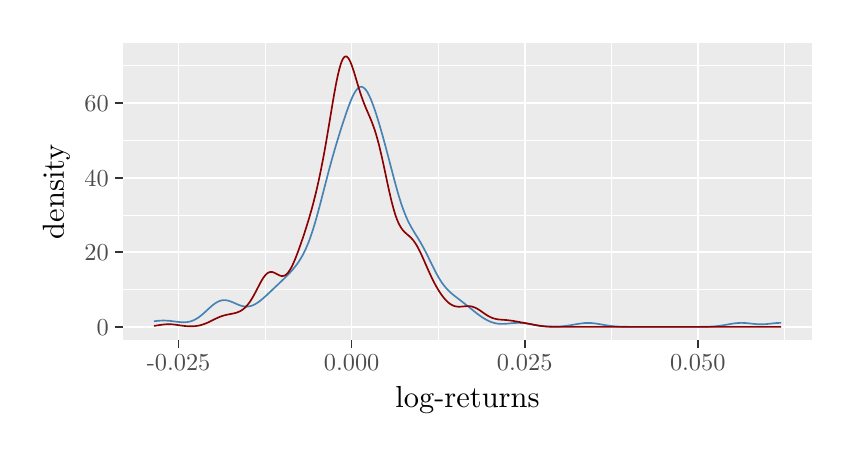
\begin{tikzpicture}[x=1pt,y=1pt]
\definecolor{fillColor}{RGB}{255,255,255}
\path[use as bounding box,fill=fillColor,fill opacity=0.00] (0,0) rectangle (289.08,144.54);
\begin{scope}
\path[clip] (  0.00,  0.00) rectangle (289.08,144.54);
\definecolor{drawColor}{RGB}{255,255,255}
\definecolor{fillColor}{RGB}{255,255,255}

\path[draw=drawColor,line width= 0.6pt,line join=round,line cap=round,fill=fillColor] (  0.00,  0.00) rectangle (289.08,144.54);
\end{scope}
\begin{scope}
\path[clip] ( 34.27, 31.53) rectangle (283.58,139.04);
\definecolor{fillColor}{gray}{0.92}

\path[fill=fillColor] ( 34.27, 31.53) rectangle (283.58,139.04);
\definecolor{drawColor}{RGB}{255,255,255}

\path[draw=drawColor,line width= 0.3pt,line join=round] ( 34.27, 49.90) --
	(283.58, 49.90);

\path[draw=drawColor,line width= 0.3pt,line join=round] ( 34.27, 76.85) --
	(283.58, 76.85);

\path[draw=drawColor,line width= 0.3pt,line join=round] ( 34.27,103.81) --
	(283.58,103.81);

\path[draw=drawColor,line width= 0.3pt,line join=round] ( 34.27,130.77) --
	(283.58,130.77);

\path[draw=drawColor,line width= 0.3pt,line join=round] ( 85.80, 31.53) --
	( 85.80,139.04);

\path[draw=drawColor,line width= 0.3pt,line join=round] (148.33, 31.53) --
	(148.33,139.04);

\path[draw=drawColor,line width= 0.3pt,line join=round] (210.86, 31.53) --
	(210.86,139.04);

\path[draw=drawColor,line width= 0.3pt,line join=round] (273.40, 31.53) --
	(273.40,139.04);

\path[draw=drawColor,line width= 0.6pt,line join=round] ( 34.27, 36.42) --
	(283.58, 36.42);

\path[draw=drawColor,line width= 0.6pt,line join=round] ( 34.27, 63.38) --
	(283.58, 63.38);

\path[draw=drawColor,line width= 0.6pt,line join=round] ( 34.27, 90.33) --
	(283.58, 90.33);

\path[draw=drawColor,line width= 0.6pt,line join=round] ( 34.27,117.29) --
	(283.58,117.29);

\path[draw=drawColor,line width= 0.6pt,line join=round] ( 54.53, 31.53) --
	( 54.53,139.04);

\path[draw=drawColor,line width= 0.6pt,line join=round] (117.07, 31.53) --
	(117.07,139.04);

\path[draw=drawColor,line width= 0.6pt,line join=round] (179.60, 31.53) --
	(179.60,139.04);

\path[draw=drawColor,line width= 0.6pt,line join=round] (242.13, 31.53) --
	(242.13,139.04);
\definecolor{drawColor}{RGB}{70,130,180}

\path[draw=drawColor,line width= 0.6pt,line join=round] ( 45.60, 38.43) --
	( 46.04, 38.49) --
	( 46.49, 38.55) --
	( 46.93, 38.60) --
	( 47.37, 38.64) --
	( 47.82, 38.67) --
	( 48.26, 38.69) --
	( 48.70, 38.71) --
	( 49.15, 38.71) --
	( 49.59, 38.70) --
	( 50.04, 38.68) --
	( 50.48, 38.66) --
	( 50.92, 38.63) --
	( 51.37, 38.59) --
	( 51.81, 38.54) --
	( 52.25, 38.49) --
	( 52.70, 38.43) --
	( 53.14, 38.38) --
	( 53.58, 38.32) --
	( 54.03, 38.26) --
	( 54.47, 38.21) --
	( 54.91, 38.17) --
	( 55.36, 38.13) --
	( 55.80, 38.10) --
	( 56.25, 38.09) --
	( 56.69, 38.10) --
	( 57.13, 38.12) --
	( 57.58, 38.16) --
	( 58.02, 38.23) --
	( 58.46, 38.32) --
	( 58.91, 38.43) --
	( 59.35, 38.58) --
	( 59.79, 38.75) --
	( 60.24, 38.95) --
	( 60.68, 39.18) --
	( 61.12, 39.44) --
	( 61.57, 39.72) --
	( 62.01, 40.03) --
	( 62.45, 40.37) --
	( 62.90, 40.73) --
	( 63.34, 41.10) --
	( 63.79, 41.49) --
	( 64.23, 41.90) --
	( 64.67, 42.31) --
	( 65.12, 42.72) --
	( 65.56, 43.13) --
	( 66.00, 43.53) --
	( 66.45, 43.92) --
	( 66.89, 44.28) --
	( 67.33, 44.63) --
	( 67.78, 44.95) --
	( 68.22, 45.23) --
	( 68.66, 45.47) --
	( 69.11, 45.68) --
	( 69.55, 45.84) --
	( 69.99, 45.97) --
	( 70.44, 46.05) --
	( 70.88, 46.09) --
	( 71.33, 46.08) --
	( 71.77, 46.03) --
	( 72.21, 45.95) --
	( 72.66, 45.84) --
	( 73.10, 45.70) --
	( 73.54, 45.54) --
	( 73.99, 45.36) --
	( 74.43, 45.16) --
	( 74.87, 44.97) --
	( 75.32, 44.77) --
	( 75.76, 44.58) --
	( 76.20, 44.40) --
	( 76.65, 44.23) --
	( 77.09, 44.08) --
	( 77.53, 43.96) --
	( 77.98, 43.87) --
	( 78.42, 43.80) --
	( 78.87, 43.77) --
	( 79.31, 43.77) --
	( 79.75, 43.80) --
	( 80.20, 43.87) --
	( 80.64, 43.98) --
	( 81.08, 44.12) --
	( 81.53, 44.30) --
	( 81.97, 44.51) --
	( 82.41, 44.75) --
	( 82.86, 45.02) --
	( 83.30, 45.32) --
	( 83.74, 45.65) --
	( 84.19, 45.99) --
	( 84.63, 46.35) --
	( 85.07, 46.73) --
	( 85.52, 47.12) --
	( 85.96, 47.52) --
	( 86.41, 47.93) --
	( 86.85, 48.35) --
	( 87.29, 48.76) --
	( 87.74, 49.18) --
	( 88.18, 49.60) --
	( 88.62, 50.02) --
	( 89.07, 50.44) --
	( 89.51, 50.86) --
	( 89.95, 51.28) --
	( 90.40, 51.70) --
	( 90.84, 52.12) --
	( 91.28, 52.54) --
	( 91.73, 52.97) --
	( 92.17, 53.39) --
	( 92.62, 53.82) --
	( 93.06, 54.26) --
	( 93.50, 54.70) --
	( 93.95, 55.15) --
	( 94.39, 55.61) --
	( 94.83, 56.08) --
	( 95.28, 56.57) --
	( 95.72, 57.07) --
	( 96.16, 57.60) --
	( 96.61, 58.15) --
	( 97.05, 58.72) --
	( 97.49, 59.33) --
	( 97.94, 59.97) --
	( 98.38, 60.65) --
	( 98.82, 61.38) --
	( 99.27, 62.16) --
	( 99.71, 63.00) --
	(100.16, 63.90) --
	(100.60, 64.86) --
	(101.04, 65.88) --
	(101.49, 66.98) --
	(101.93, 68.16) --
	(102.37, 69.42) --
	(102.82, 70.74) --
	(103.26, 72.13) --
	(103.70, 73.58) --
	(104.15, 75.10) --
	(104.59, 76.68) --
	(105.03, 78.31) --
	(105.48, 79.97) --
	(105.92, 81.66) --
	(106.36, 83.38) --
	(106.81, 85.10) --
	(107.25, 86.83) --
	(107.70, 88.56) --
	(108.14, 90.27) --
	(108.58, 91.96) --
	(109.03, 93.63) --
	(109.47, 95.27) --
	(109.91, 96.88) --
	(110.36, 98.45) --
	(110.80,100.00) --
	(111.24,101.51) --
	(111.69,103.00) --
	(112.13,104.46) --
	(112.57,105.90) --
	(113.02,107.32) --
	(113.46,108.72) --
	(113.90,110.09) --
	(114.35,111.44) --
	(114.79,112.77) --
	(115.24,114.07) --
	(115.68,115.32) --
	(116.12,116.53) --
	(116.57,117.68) --
	(117.01,118.75) --
	(117.45,119.73) --
	(117.90,120.61) --
	(118.34,121.38) --
	(118.78,122.04) --
	(119.23,122.56) --
	(119.67,122.93) --
	(120.11,123.13) --
	(120.56,123.18) --
	(121.00,123.08) --
	(121.45,122.83) --
	(121.89,122.43) --
	(122.33,121.89) --
	(122.78,121.20) --
	(123.22,120.37) --
	(123.66,119.44) --
	(124.11,118.41) --
	(124.55,117.28) --
	(124.99,116.08) --
	(125.44,114.80) --
	(125.88,113.46) --
	(126.32,112.06) --
	(126.77,110.62) --
	(127.21,109.13) --
	(127.65,107.61) --
	(128.10,106.05) --
	(128.54,104.46) --
	(128.99,102.83) --
	(129.43,101.18) --
	(129.87, 99.51) --
	(130.32, 97.83) --
	(130.76, 96.13) --
	(131.20, 94.42) --
	(131.65, 92.72) --
	(132.09, 91.03) --
	(132.53, 89.36) --
	(132.98, 87.72) --
	(133.42, 86.13) --
	(133.86, 84.58) --
	(134.31, 83.09) --
	(134.75, 81.67) --
	(135.19, 80.32) --
	(135.64, 79.06) --
	(136.08, 77.87) --
	(136.53, 76.76) --
	(136.97, 75.72) --
	(137.41, 74.75) --
	(137.86, 73.85) --
	(138.30, 73.01) --
	(138.74, 72.22) --
	(139.19, 71.46) --
	(139.63, 70.73) --
	(140.07, 70.01) --
	(140.52, 69.30) --
	(140.96, 68.59) --
	(141.40, 67.86) --
	(141.85, 67.11) --
	(142.29, 66.34) --
	(142.73, 65.55) --
	(143.18, 64.73) --
	(143.62, 63.88) --
	(144.07, 63.01) --
	(144.51, 62.12) --
	(144.95, 61.21) --
	(145.40, 60.30) --
	(145.84, 59.38) --
	(146.28, 58.48) --
	(146.73, 57.58) --
	(147.17, 56.71) --
	(147.61, 55.87) --
	(148.06, 55.05) --
	(148.50, 54.28) --
	(148.94, 53.54) --
	(149.39, 52.84) --
	(149.83, 52.19) --
	(150.27, 51.59) --
	(150.72, 51.02) --
	(151.16, 50.50) --
	(151.61, 50.01) --
	(152.05, 49.55) --
	(152.49, 49.12) --
	(152.94, 48.71) --
	(153.38, 48.33) --
	(153.82, 47.97) --
	(154.27, 47.61) --
	(154.71, 47.27) --
	(155.15, 46.93) --
	(155.60, 46.59) --
	(156.04, 46.25) --
	(156.48, 45.92) --
	(156.93, 45.57) --
	(157.37, 45.23) --
	(157.82, 44.88) --
	(158.26, 44.53) --
	(158.70, 44.18) --
	(159.15, 43.82) --
	(159.59, 43.46) --
	(160.03, 43.10) --
	(160.48, 42.74) --
	(160.92, 42.38) --
	(161.36, 42.03) --
	(161.81, 41.68) --
	(162.25, 41.33) --
	(162.69, 41.00) --
	(163.14, 40.67) --
	(163.58, 40.35) --
	(164.02, 40.05) --
	(164.47, 39.75) --
	(164.91, 39.47) --
	(165.36, 39.21) --
	(165.80, 38.96) --
	(166.24, 38.73) --
	(166.69, 38.52) --
	(167.13, 38.33) --
	(167.57, 38.16) --
	(168.02, 38.00) --
	(168.46, 37.88) --
	(168.90, 37.77) --
	(169.35, 37.68) --
	(169.79, 37.60) --
	(170.23, 37.55) --
	(170.68, 37.52) --
	(171.12, 37.50) --
	(171.56, 37.50) --
	(172.01, 37.51) --
	(172.45, 37.53) --
	(172.90, 37.56) --
	(173.34, 37.59) --
	(173.78, 37.63) --
	(174.23, 37.68) --
	(174.67, 37.72) --
	(175.11, 37.76) --
	(175.56, 37.79) --
	(176.00, 37.82) --
	(176.44, 37.85) --
	(176.89, 37.86) --
	(177.33, 37.86) --
	(177.77, 37.86) --
	(178.22, 37.84) --
	(178.66, 37.81) --
	(179.10, 37.77) --
	(179.55, 37.72) --
	(179.99, 37.67) --
	(180.44, 37.61) --
	(180.88, 37.54) --
	(181.32, 37.46) --
	(181.77, 37.38) --
	(182.21, 37.31) --
	(182.65, 37.23) --
	(183.10, 37.15) --
	(183.54, 37.07) --
	(183.98, 37.00) --
	(184.43, 36.93) --
	(184.87, 36.87) --
	(185.31, 36.81) --
	(185.76, 36.76) --
	(186.20, 36.71) --
	(186.64, 36.67) --
	(187.09, 36.63) --
	(187.53, 36.60) --
	(187.98, 36.57) --
	(188.42, 36.55) --
	(188.86, 36.54) --
	(189.31, 36.53) --
	(189.75, 36.52) --
	(190.19, 36.52) --
	(190.64, 36.53) --
	(191.08, 36.54) --
	(191.52, 36.55) --
	(191.97, 36.57) --
	(192.41, 36.60) --
	(192.85, 36.63) --
	(193.30, 36.66) --
	(193.74, 36.70) --
	(194.19, 36.75) --
	(194.63, 36.80) --
	(195.07, 36.86) --
	(195.52, 36.93) --
	(195.96, 36.99) --
	(196.40, 37.07) --
	(196.85, 37.14) --
	(197.29, 37.22) --
	(197.73, 37.30) --
	(198.18, 37.38) --
	(198.62, 37.45) --
	(199.06, 37.53) --
	(199.51, 37.59) --
	(199.95, 37.66) --
	(200.39, 37.71) --
	(200.84, 37.76) --
	(201.28, 37.80) --
	(201.73, 37.82) --
	(202.17, 37.84) --
	(202.61, 37.84) --
	(203.06, 37.83) --
	(203.50, 37.81) --
	(203.94, 37.78) --
	(204.39, 37.74) --
	(204.83, 37.69) --
	(205.27, 37.63) --
	(205.72, 37.57) --
	(206.16, 37.49) --
	(206.60, 37.42) --
	(207.05, 37.34) --
	(207.49, 37.26) --
	(207.93, 37.18) --
	(208.38, 37.11) --
	(208.82, 37.03) --
	(209.27, 36.96) --
	(209.71, 36.90) --
	(210.15, 36.83) --
	(210.60, 36.78) --
	(211.04, 36.73) --
	(211.48, 36.68) --
	(211.93, 36.64) --
	(212.37, 36.60) --
	(212.81, 36.57) --
	(213.26, 36.54) --
	(213.70, 36.52) --
	(214.14, 36.50) --
	(214.59, 36.48) --
	(215.03, 36.47) --
	(215.47, 36.46) --
	(215.92, 36.45) --
	(216.36, 36.44) --
	(216.81, 36.44) --
	(217.25, 36.43) --
	(217.69, 36.43) --
	(218.14, 36.43) --
	(218.58, 36.42) --
	(219.02, 36.42) --
	(219.47, 36.42) --
	(219.91, 36.42) --
	(220.35, 36.42) --
	(220.80, 36.42) --
	(221.24, 36.42) --
	(221.68, 36.42) --
	(222.13, 36.42) --
	(222.57, 36.42) --
	(223.02, 36.42) --
	(223.46, 36.42) --
	(223.90, 36.42) --
	(224.35, 36.42) --
	(224.79, 36.42) --
	(225.23, 36.42) --
	(225.68, 36.42) --
	(226.12, 36.42) --
	(226.56, 36.42) --
	(227.01, 36.42) --
	(227.45, 36.42) --
	(227.89, 36.42) --
	(228.34, 36.42) --
	(228.78, 36.42) --
	(229.22, 36.42) --
	(229.67, 36.42) --
	(230.11, 36.42) --
	(230.56, 36.42) --
	(231.00, 36.42) --
	(231.44, 36.42) --
	(231.89, 36.42) --
	(232.33, 36.42) --
	(232.77, 36.42) --
	(233.22, 36.42) --
	(233.66, 36.42) --
	(234.10, 36.42) --
	(234.55, 36.42) --
	(234.99, 36.42) --
	(235.43, 36.42) --
	(235.88, 36.42) --
	(236.32, 36.42) --
	(236.76, 36.42) --
	(237.21, 36.42) --
	(237.65, 36.42) --
	(238.10, 36.42) --
	(238.54, 36.42) --
	(238.98, 36.42) --
	(239.43, 36.42) --
	(239.87, 36.42) --
	(240.31, 36.42) --
	(240.76, 36.42) --
	(241.20, 36.42) --
	(241.64, 36.42) --
	(242.09, 36.43) --
	(242.53, 36.43) --
	(242.97, 36.43) --
	(243.42, 36.44) --
	(243.86, 36.44) --
	(244.30, 36.45) --
	(244.75, 36.46) --
	(245.19, 36.47) --
	(245.64, 36.48) --
	(246.08, 36.50) --
	(246.52, 36.52) --
	(246.97, 36.54) --
	(247.41, 36.57) --
	(247.85, 36.60) --
	(248.30, 36.63) --
	(248.74, 36.67) --
	(249.18, 36.72) --
	(249.63, 36.77) --
	(250.07, 36.83) --
	(250.51, 36.89) --
	(250.96, 36.95) --
	(251.40, 37.02) --
	(251.84, 37.10) --
	(252.29, 37.17) --
	(252.73, 37.25) --
	(253.18, 37.33) --
	(253.62, 37.41) --
	(254.06, 37.49) --
	(254.51, 37.56) --
	(254.95, 37.63) --
	(255.39, 37.69) --
	(255.84, 37.74) --
	(256.28, 37.79) --
	(256.72, 37.82) --
	(257.17, 37.84) --
	(257.61, 37.86) --
	(258.05, 37.86) --
	(258.50, 37.85) --
	(258.94, 37.84) --
	(259.39, 37.81) --
	(259.83, 37.78) --
	(260.27, 37.74) --
	(260.72, 37.69) --
	(261.16, 37.64) --
	(261.60, 37.59) --
	(262.05, 37.54) --
	(262.49, 37.50) --
	(262.93, 37.46) --
	(263.38, 37.42) --
	(263.82, 37.39) --
	(264.26, 37.37) --
	(264.71, 37.36) --
	(265.15, 37.36) --
	(265.59, 37.37) --
	(266.04, 37.39) --
	(266.48, 37.41) --
	(266.93, 37.44) --
	(267.37, 37.48) --
	(267.81, 37.53) --
	(268.26, 37.58) --
	(268.70, 37.62) --
	(269.14, 37.67) --
	(269.59, 37.72) --
	(270.03, 37.76) --
	(270.47, 37.80) --
	(270.92, 37.83) --
	(271.36, 37.85) --
	(271.80, 37.86) --
	(272.25, 37.86);
\definecolor{drawColor}{RGB}{139,0,0}

\path[draw=drawColor,line width= 0.6pt,line join=round] ( 45.60, 36.78) --
	( 46.04, 36.84) --
	( 46.49, 36.90) --
	( 46.93, 36.97) --
	( 47.37, 37.04) --
	( 47.82, 37.10) --
	( 48.26, 37.17) --
	( 48.70, 37.22) --
	( 49.15, 37.27) --
	( 49.59, 37.32) --
	( 50.04, 37.35) --
	( 50.48, 37.37) --
	( 50.92, 37.38) --
	( 51.37, 37.37) --
	( 51.81, 37.36) --
	( 52.25, 37.33) --
	( 52.70, 37.29) --
	( 53.14, 37.24) --
	( 53.58, 37.18) --
	( 54.03, 37.12) --
	( 54.47, 37.05) --
	( 54.91, 36.99) --
	( 55.36, 36.92) --
	( 55.80, 36.86) --
	( 56.25, 36.81) --
	( 56.69, 36.75) --
	( 57.13, 36.71) --
	( 57.58, 36.67) --
	( 58.02, 36.65) --
	( 58.46, 36.63) --
	( 58.91, 36.62) --
	( 59.35, 36.63) --
	( 59.79, 36.65) --
	( 60.24, 36.68) --
	( 60.68, 36.72) --
	( 61.12, 36.78) --
	( 61.57, 36.85) --
	( 62.01, 36.93) --
	( 62.45, 37.04) --
	( 62.90, 37.16) --
	( 63.34, 37.30) --
	( 63.79, 37.45) --
	( 64.23, 37.62) --
	( 64.67, 37.80) --
	( 65.12, 38.00) --
	( 65.56, 38.20) --
	( 66.00, 38.42) --
	( 66.45, 38.64) --
	( 66.89, 38.86) --
	( 67.33, 39.08) --
	( 67.78, 39.30) --
	( 68.22, 39.51) --
	( 68.66, 39.72) --
	( 69.11, 39.91) --
	( 69.55, 40.09) --
	( 69.99, 40.25) --
	( 70.44, 40.40) --
	( 70.88, 40.54) --
	( 71.33, 40.66) --
	( 71.77, 40.76) --
	( 72.21, 40.86) --
	( 72.66, 40.95) --
	( 73.10, 41.03) --
	( 73.54, 41.11) --
	( 73.99, 41.20) --
	( 74.43, 41.29) --
	( 74.87, 41.40) --
	( 75.32, 41.52) --
	( 75.76, 41.67) --
	( 76.20, 41.84) --
	( 76.65, 42.04) --
	( 77.09, 42.28) --
	( 77.53, 42.57) --
	( 77.98, 42.90) --
	( 78.42, 43.28) --
	( 78.87, 43.72) --
	( 79.31, 44.20) --
	( 79.75, 44.74) --
	( 80.20, 45.34) --
	( 80.64, 46.00) --
	( 81.08, 46.71) --
	( 81.53, 47.48) --
	( 81.97, 48.29) --
	( 82.41, 49.12) --
	( 82.86, 49.98) --
	( 83.30, 50.84) --
	( 83.74, 51.70) --
	( 84.19, 52.53) --
	( 84.63, 53.31) --
	( 85.07, 54.02) --
	( 85.52, 54.66) --
	( 85.96, 55.19) --
	( 86.41, 55.63) --
	( 86.85, 55.95) --
	( 87.29, 56.17) --
	( 87.74, 56.27) --
	( 88.18, 56.28) --
	( 88.62, 56.18) --
	( 89.07, 56.01) --
	( 89.51, 55.80) --
	( 89.95, 55.56) --
	( 90.40, 55.32) --
	( 90.84, 55.09) --
	( 91.28, 54.92) --
	( 91.73, 54.81) --
	( 92.17, 54.79) --
	( 92.62, 54.88) --
	( 93.06, 55.09) --
	( 93.50, 55.41) --
	( 93.95, 55.86) --
	( 94.39, 56.42) --
	( 94.83, 57.10) --
	( 95.28, 57.89) --
	( 95.72, 58.78) --
	( 96.16, 59.76) --
	( 96.61, 60.82) --
	( 97.05, 61.93) --
	( 97.49, 63.10) --
	( 97.94, 64.30) --
	( 98.38, 65.54) --
	( 98.82, 66.81) --
	( 99.27, 68.10) --
	( 99.71, 69.43) --
	(100.16, 70.78) --
	(100.60, 72.16) --
	(101.04, 73.57) --
	(101.49, 75.02) --
	(101.93, 76.52) --
	(102.37, 78.07) --
	(102.82, 79.67) --
	(103.26, 81.34) --
	(103.70, 83.07) --
	(104.15, 84.88) --
	(104.59, 86.77) --
	(105.03, 88.74) --
	(105.48, 90.79) --
	(105.92, 92.92) --
	(106.36, 95.15) --
	(106.81, 97.47) --
	(107.25, 99.88) --
	(107.70,102.38) --
	(108.14,104.95) --
	(108.58,107.58) --
	(109.03,110.24) --
	(109.47,112.93) --
	(109.91,115.61) --
	(110.36,118.25) --
	(110.80,120.80) --
	(111.24,123.23) --
	(111.69,125.50) --
	(112.13,127.57) --
	(112.57,129.41) --
	(113.02,130.99) --
	(113.46,132.27) --
	(113.90,133.25) --
	(114.35,133.88) --
	(114.79,134.15) --
	(115.24,134.11) --
	(115.68,133.76) --
	(116.12,133.14) --
	(116.57,132.27) --
	(117.01,131.19) --
	(117.45,129.94) --
	(117.90,128.57) --
	(118.34,127.11) --
	(118.78,125.61) --
	(119.23,124.12) --
	(119.67,122.65) --
	(120.11,121.24) --
	(120.56,119.89) --
	(121.00,118.62) --
	(121.45,117.42) --
	(121.89,116.30) --
	(122.33,115.24) --
	(122.78,114.20) --
	(123.22,113.18) --
	(123.66,112.15) --
	(124.11,111.08) --
	(124.55,109.95) --
	(124.99,108.75) --
	(125.44,107.46) --
	(125.88,106.04) --
	(126.32,104.50) --
	(126.77,102.85) --
	(127.21,101.08) --
	(127.65, 99.21) --
	(128.10, 97.26) --
	(128.54, 95.23) --
	(128.99, 93.15) --
	(129.43, 91.05) --
	(129.87, 88.96) --
	(130.32, 86.90) --
	(130.76, 84.91) --
	(131.20, 82.99) --
	(131.65, 81.19) --
	(132.09, 79.50) --
	(132.53, 77.96) --
	(132.98, 76.57) --
	(133.42, 75.34) --
	(133.86, 74.27) --
	(134.31, 73.35) --
	(134.75, 72.55) --
	(135.19, 71.88) --
	(135.64, 71.30) --
	(136.08, 70.81) --
	(136.53, 70.38) --
	(136.97, 69.99) --
	(137.41, 69.62) --
	(137.86, 69.23) --
	(138.30, 68.82) --
	(138.74, 68.37) --
	(139.19, 67.86) --
	(139.63, 67.29) --
	(140.07, 66.66) --
	(140.52, 65.95) --
	(140.96, 65.17) --
	(141.40, 64.33) --
	(141.85, 63.44) --
	(142.29, 62.50) --
	(142.73, 61.52) --
	(143.18, 60.52) --
	(143.62, 59.50) --
	(144.07, 58.48) --
	(144.51, 57.47) --
	(144.95, 56.47) --
	(145.40, 55.50) --
	(145.84, 54.55) --
	(146.28, 53.63) --
	(146.73, 52.75) --
	(147.17, 51.90) --
	(147.61, 51.09) --
	(148.06, 50.32) --
	(148.50, 49.59) --
	(148.94, 48.90) --
	(149.39, 48.24) --
	(149.83, 47.63) --
	(150.27, 47.05) --
	(150.72, 46.52) --
	(151.16, 46.03) --
	(151.61, 45.58) --
	(152.05, 45.19) --
	(152.49, 44.84) --
	(152.94, 44.54) --
	(153.38, 44.29) --
	(153.82, 44.09) --
	(154.27, 43.93) --
	(154.71, 43.82) --
	(155.15, 43.75) --
	(155.60, 43.71) --
	(156.04, 43.71) --
	(156.48, 43.73) --
	(156.93, 43.76) --
	(157.37, 43.81) --
	(157.82, 43.85) --
	(158.26, 43.89) --
	(158.70, 43.92) --
	(159.15, 43.92) --
	(159.59, 43.90) --
	(160.03, 43.85) --
	(160.48, 43.77) --
	(160.92, 43.65) --
	(161.36, 43.49) --
	(161.81, 43.30) --
	(162.25, 43.08) --
	(162.69, 42.83) --
	(163.14, 42.56) --
	(163.58, 42.26) --
	(164.02, 41.95) --
	(164.47, 41.64) --
	(164.91, 41.33) --
	(165.36, 41.02) --
	(165.80, 40.73) --
	(166.24, 40.46) --
	(166.69, 40.20) --
	(167.13, 39.98) --
	(167.57, 39.78) --
	(168.02, 39.60) --
	(168.46, 39.46) --
	(168.90, 39.34) --
	(169.35, 39.24) --
	(169.79, 39.16) --
	(170.23, 39.10) --
	(170.68, 39.06) --
	(171.12, 39.02) --
	(171.56, 38.99) --
	(172.01, 38.96) --
	(172.45, 38.93) --
	(172.90, 38.89) --
	(173.34, 38.85) --
	(173.78, 38.80) --
	(174.23, 38.75) --
	(174.67, 38.69) --
	(175.11, 38.62) --
	(175.56, 38.55) --
	(176.00, 38.48) --
	(176.44, 38.40) --
	(176.89, 38.32) --
	(177.33, 38.24) --
	(177.77, 38.16) --
	(178.22, 38.08) --
	(178.66, 38.00) --
	(179.10, 37.92) --
	(179.55, 37.84) --
	(179.99, 37.76) --
	(180.44, 37.68) --
	(180.88, 37.59) --
	(181.32, 37.50) --
	(181.77, 37.42) --
	(182.21, 37.33) --
	(182.65, 37.24) --
	(183.10, 37.16) --
	(183.54, 37.07) --
	(183.98, 36.99) --
	(184.43, 36.91) --
	(184.87, 36.84) --
	(185.31, 36.78) --
	(185.76, 36.72) --
	(186.20, 36.67) --
	(186.64, 36.62) --
	(187.09, 36.58) --
	(187.53, 36.55) --
	(187.98, 36.52) --
	(188.42, 36.50) --
	(188.86, 36.48) --
	(189.31, 36.46) --
	(189.75, 36.45) --
	(190.19, 36.44) --
	(190.64, 36.44) --
	(191.08, 36.43) --
	(191.52, 36.43) --
	(191.97, 36.42) --
	(192.41, 36.42) --
	(192.85, 36.42) --
	(193.30, 36.42) --
	(193.74, 36.42) --
	(194.19, 36.42) --
	(194.63, 36.42) --
	(195.07, 36.42) --
	(195.52, 36.42) --
	(195.96, 36.42) --
	(196.40, 36.42) --
	(196.85, 36.42) --
	(197.29, 36.42) --
	(197.73, 36.42) --
	(198.18, 36.42) --
	(198.62, 36.42) --
	(199.06, 36.42) --
	(199.51, 36.42) --
	(199.95, 36.42) --
	(200.39, 36.42) --
	(200.84, 36.42) --
	(201.28, 36.42) --
	(201.73, 36.42) --
	(202.17, 36.42) --
	(202.61, 36.42) --
	(203.06, 36.42) --
	(203.50, 36.42) --
	(203.94, 36.42) --
	(204.39, 36.42) --
	(204.83, 36.42) --
	(205.27, 36.42) --
	(205.72, 36.42) --
	(206.16, 36.42) --
	(206.60, 36.42) --
	(207.05, 36.42) --
	(207.49, 36.42) --
	(207.93, 36.42) --
	(208.38, 36.42) --
	(208.82, 36.42) --
	(209.27, 36.42) --
	(209.71, 36.42) --
	(210.15, 36.42) --
	(210.60, 36.42) --
	(211.04, 36.42) --
	(211.48, 36.42) --
	(211.93, 36.42) --
	(212.37, 36.42) --
	(212.81, 36.42) --
	(213.26, 36.42) --
	(213.70, 36.42) --
	(214.14, 36.42) --
	(214.59, 36.42) --
	(215.03, 36.42) --
	(215.47, 36.42) --
	(215.92, 36.42) --
	(216.36, 36.42) --
	(216.81, 36.42) --
	(217.25, 36.42) --
	(217.69, 36.42) --
	(218.14, 36.42) --
	(218.58, 36.42) --
	(219.02, 36.42) --
	(219.47, 36.42) --
	(219.91, 36.42) --
	(220.35, 36.42) --
	(220.80, 36.42) --
	(221.24, 36.42) --
	(221.68, 36.42) --
	(222.13, 36.42) --
	(222.57, 36.42) --
	(223.02, 36.42) --
	(223.46, 36.42) --
	(223.90, 36.42) --
	(224.35, 36.42) --
	(224.79, 36.42) --
	(225.23, 36.42) --
	(225.68, 36.42) --
	(226.12, 36.42) --
	(226.56, 36.42) --
	(227.01, 36.42) --
	(227.45, 36.42) --
	(227.89, 36.42) --
	(228.34, 36.42) --
	(228.78, 36.42) --
	(229.22, 36.42) --
	(229.67, 36.42) --
	(230.11, 36.42) --
	(230.56, 36.42) --
	(231.00, 36.42) --
	(231.44, 36.42) --
	(231.89, 36.42) --
	(232.33, 36.42) --
	(232.77, 36.42) --
	(233.22, 36.42) --
	(233.66, 36.42) --
	(234.10, 36.42) --
	(234.55, 36.42) --
	(234.99, 36.42) --
	(235.43, 36.42) --
	(235.88, 36.42) --
	(236.32, 36.42) --
	(236.76, 36.42) --
	(237.21, 36.42) --
	(237.65, 36.42) --
	(238.10, 36.42) --
	(238.54, 36.42) --
	(238.98, 36.42) --
	(239.43, 36.42) --
	(239.87, 36.42) --
	(240.31, 36.42) --
	(240.76, 36.42) --
	(241.20, 36.42) --
	(241.64, 36.42) --
	(242.09, 36.42) --
	(242.53, 36.42) --
	(242.97, 36.42) --
	(243.42, 36.42) --
	(243.86, 36.42) --
	(244.30, 36.42) --
	(244.75, 36.42) --
	(245.19, 36.42) --
	(245.64, 36.42) --
	(246.08, 36.42) --
	(246.52, 36.42) --
	(246.97, 36.42) --
	(247.41, 36.42) --
	(247.85, 36.42) --
	(248.30, 36.42) --
	(248.74, 36.42) --
	(249.18, 36.42) --
	(249.63, 36.42) --
	(250.07, 36.42) --
	(250.51, 36.42) --
	(250.96, 36.42) --
	(251.40, 36.42) --
	(251.84, 36.42) --
	(252.29, 36.42) --
	(252.73, 36.42) --
	(253.18, 36.42) --
	(253.62, 36.42) --
	(254.06, 36.42) --
	(254.51, 36.42) --
	(254.95, 36.42) --
	(255.39, 36.42) --
	(255.84, 36.42) --
	(256.28, 36.42) --
	(256.72, 36.42) --
	(257.17, 36.42) --
	(257.61, 36.42) --
	(258.05, 36.42) --
	(258.50, 36.42) --
	(258.94, 36.42) --
	(259.39, 36.42) --
	(259.83, 36.42) --
	(260.27, 36.42) --
	(260.72, 36.42) --
	(261.16, 36.42) --
	(261.60, 36.42) --
	(262.05, 36.42) --
	(262.49, 36.42) --
	(262.93, 36.42) --
	(263.38, 36.42) --
	(263.82, 36.42) --
	(264.26, 36.42) --
	(264.71, 36.42) --
	(265.15, 36.42) --
	(265.59, 36.42) --
	(266.04, 36.42) --
	(266.48, 36.42) --
	(266.93, 36.42) --
	(267.37, 36.42) --
	(267.81, 36.42) --
	(268.26, 36.42) --
	(268.70, 36.42) --
	(269.14, 36.42) --
	(269.59, 36.42) --
	(270.03, 36.42) --
	(270.47, 36.42) --
	(270.92, 36.42) --
	(271.36, 36.42) --
	(271.80, 36.42) --
	(272.25, 36.42);
\end{scope}
\begin{scope}
\path[clip] (  0.00,  0.00) rectangle (289.08,144.54);
\definecolor{drawColor}{gray}{0.30}

\node[text=drawColor,anchor=base east,inner sep=0pt, outer sep=0pt, scale=  0.88] at ( 29.32, 33.39) {0};

\node[text=drawColor,anchor=base east,inner sep=0pt, outer sep=0pt, scale=  0.88] at ( 29.32, 60.34) {20};

\node[text=drawColor,anchor=base east,inner sep=0pt, outer sep=0pt, scale=  0.88] at ( 29.32, 87.30) {40};

\node[text=drawColor,anchor=base east,inner sep=0pt, outer sep=0pt, scale=  0.88] at ( 29.32,114.26) {60};
\end{scope}
\begin{scope}
\path[clip] (  0.00,  0.00) rectangle (289.08,144.54);
\definecolor{drawColor}{gray}{0.20}

\path[draw=drawColor,line width= 0.6pt,line join=round] ( 31.52, 36.42) --
	( 34.27, 36.42);

\path[draw=drawColor,line width= 0.6pt,line join=round] ( 31.52, 63.38) --
	( 34.27, 63.38);

\path[draw=drawColor,line width= 0.6pt,line join=round] ( 31.52, 90.33) --
	( 34.27, 90.33);

\path[draw=drawColor,line width= 0.6pt,line join=round] ( 31.52,117.29) --
	( 34.27,117.29);
\end{scope}
\begin{scope}
\path[clip] (  0.00,  0.00) rectangle (289.08,144.54);
\definecolor{drawColor}{gray}{0.20}

\path[draw=drawColor,line width= 0.6pt,line join=round] ( 54.53, 28.78) --
	( 54.53, 31.53);

\path[draw=drawColor,line width= 0.6pt,line join=round] (117.07, 28.78) --
	(117.07, 31.53);

\path[draw=drawColor,line width= 0.6pt,line join=round] (179.60, 28.78) --
	(179.60, 31.53);

\path[draw=drawColor,line width= 0.6pt,line join=round] (242.13, 28.78) --
	(242.13, 31.53);
\end{scope}
\begin{scope}
\path[clip] (  0.00,  0.00) rectangle (289.08,144.54);
\definecolor{drawColor}{gray}{0.30}

\node[text=drawColor,anchor=base,inner sep=0pt, outer sep=0pt, scale=  0.88] at ( 54.53, 20.52) {-0.025};

\node[text=drawColor,anchor=base,inner sep=0pt, outer sep=0pt, scale=  0.88] at (117.07, 20.52) {0.000};

\node[text=drawColor,anchor=base,inner sep=0pt, outer sep=0pt, scale=  0.88] at (179.60, 20.52) {0.025};

\node[text=drawColor,anchor=base,inner sep=0pt, outer sep=0pt, scale=  0.88] at (242.13, 20.52) {0.050};
\end{scope}
\begin{scope}
\path[clip] (  0.00,  0.00) rectangle (289.08,144.54);
\definecolor{drawColor}{RGB}{0,0,0}

\node[text=drawColor,anchor=base,inner sep=0pt, outer sep=0pt, scale=  1.10] at (158.92,  7.44) {log-returns};
\end{scope}
\begin{scope}
\path[clip] (  0.00,  0.00) rectangle (289.08,144.54);
\definecolor{drawColor}{RGB}{0,0,0}

\node[text=drawColor,rotate= 90.00,anchor=base,inner sep=0pt, outer sep=0pt, scale=  1.10] at ( 13.08, 85.29) {density};
\end{scope}
\end{tikzpicture}

  \caption{Historical and HSV related Apple stock Log-returns distribution}
  \floatfoot{The above blue density curve is constructed over the historical data of the Apple share of stock price evolution from 18th May 2017 to 18th May 2018. while the red curve is constructed from time-series genereated by the function \textit{hsv\_ts} taking the risk-neutral parameters \ref{eq:methodology:arg:heston:riskneutral} as arguments.
  }
  \label{p:methodology:density:aapl:heston:riskneutral}
\end{figure}


The goal of that section is to find the risk-averse parameters that make both the distributions of the log-returns generated from market data or from \textit{hsv\_ts} fit together.
To do so, and according to the differences between \cref{eq:other:hsvstock:riskless,eq:other:hsvvol:riskless} from \cref{eq:other:hsvstock,eq:other:hsvvol}, the parameters to modify are the drift rate $r \to \alpha$, the mean reversion speed $\kappa^{*} \to \kappa$ and the long-run volatility $\theta^* \to \theta$.
Accordingly, the correlation parameter $\rho$ and the volatility of the volatility $\sigma$ stay unchanged from the risk-neutral to risk-averse world.

I followed the method exhibited at \cref{sec:upstream:logreturn} to get a rough estimation of the drift rate $\alpha$. From the log-returns' first and second moments, I find the value 0.4822917 for the estimate of $\alpha$.

According to \cref{eq:other:kappa:riskless,eq:other:theta:riskless}, in order to  calculate $\kappa$ and $\theta$, the risk premium $\lambda$ has to be guessed.
Practically, to do so, I am using an approximation algorithm developed by \citet{MASS} which is directly available in the R language through the function \textit{fitdistr} from the R package \textit{MASS}. 
The goal of that algorithm is the find the parameters of a density function that make it reproduce the distribution of a sample of data.
To do the job, that algorithm needs (i) a density function to be fitted along with (ii) a sample of random data as a template.
As defined in \citet{Adrian}, the density of the log-returns generated by the HSV model is given by \cref{methodology:density:heston:log}.

\begin{align}
P_t(x) &= \frac{1}{2 \pi} \int_{-\infty}^{\infty} e^{i \phi x + F_t(\phi)} d\phi \label{methodology:density:heston:log} \\
\intertext{where}
F_t(\phi) &= \frac{\kappa \theta}{\sigma^2} \gamma t -
  \frac{2 \kappa \theta}{\sigma ^2} \ln\left(
    \cosh \frac{\Omega t}{2} +
    \frac{\Omega^2 - \gamma^2 +2 \kappa \gamma}{2 \kappa \Omega} \sinh \frac{\Omega t}{2}
  \right) \notag \\
\intertext{and}
\Omega &= \sqrt{\gamma^2 + \sigma^2 (\phi^2 - i\phi)}, \notag
\gamma = \kappa + i \rho \phi \sigma \notag
\end{align}

By applying the optimization function together with \cref{methodology:density:heston:log} as a density function, the Apple stock data [REF] as a template and the variable $\lambda$ as a cursor, the optimization algorithm outputs $\lambda = 5.4883278229$ as the best fit argument for the risk premium.
Therefore, the set of the risk-averse parameters is fully described here below in \ref{eq:methodology:arg:heston:riskaverse}.

\begin{align}
  \left \{
  \begin{array}{lcl}
    V(0) &= &0.03798218, \\
    \theta &= &0.02054013, \\
    \sigma &= &0.50378803, \\
    \rho &= &-0.39877827, \\
    \kappa &= &9.489383, \\
    \alpha & = &0.4822917
  \end{array}
  \right \}  
  \label{eq:methodology:arg:heston:riskaverse}
\end{align}


\Cref{p:methodology:density:aapl:heston:riskaverse} shows the empirical density curves illustrating the distributions of the log-returns computed either from historical Apple stock data for the blue curve or from dummy time series generated by the function \textit{hsv\_ts()} fed with the risk-averse parameters\ref{eq:methodology:arg:heston:riskaverse}, for the red one.


\begin{figure}[ht]
  \centering
  % Created by tikzDevice version 0.11 on 2018-07-18 23:47:53
% !TEX encoding = UTF-8 Unicode
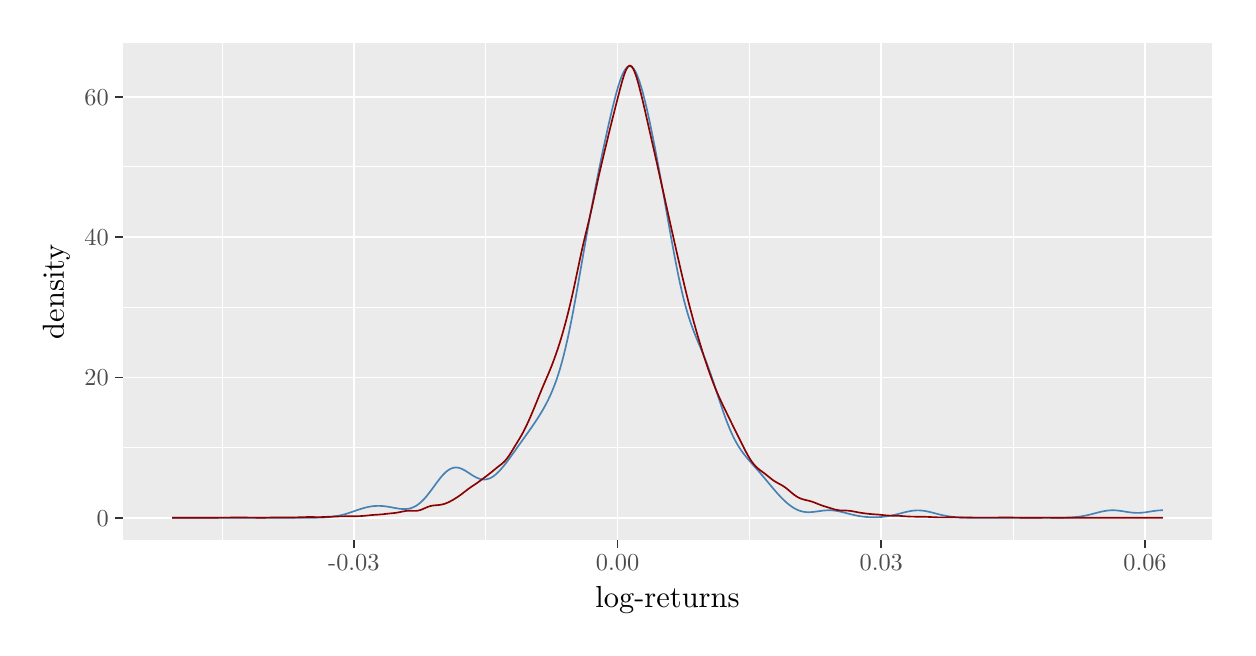
\begin{tikzpicture}[x=1pt,y=1pt]
\definecolor{fillColor}{RGB}{255,255,255}
\path[use as bounding box,fill=fillColor,fill opacity=0.00] (0,0) rectangle (433.62,216.81);
\begin{scope}
\path[clip] (  0.00,  0.00) rectangle (433.62,216.81);
\definecolor{drawColor}{RGB}{255,255,255}
\definecolor{fillColor}{RGB}{255,255,255}

\path[draw=drawColor,line width= 0.6pt,line join=round,line cap=round,fill=fillColor] (  0.00,  0.00) rectangle (433.62,216.81);
\end{scope}
\begin{scope}
\path[clip] ( 34.27, 31.53) rectangle (428.12,211.31);
\definecolor{fillColor}{gray}{0.92}

\path[fill=fillColor] ( 34.27, 31.53) rectangle (428.12,211.31);
\definecolor{drawColor}{RGB}{255,255,255}

\path[draw=drawColor,line width= 0.3pt,line join=round] ( 34.27, 65.06) --
	(428.12, 65.06);

\path[draw=drawColor,line width= 0.3pt,line join=round] ( 34.27,115.78) --
	(428.12,115.78);

\path[draw=drawColor,line width= 0.3pt,line join=round] ( 34.27,166.50) --
	(428.12,166.50);

\path[draw=drawColor,line width= 0.3pt,line join=round] ( 70.24, 31.53) --
	( 70.24,211.31);

\path[draw=drawColor,line width= 0.3pt,line join=round] (165.52, 31.53) --
	(165.52,211.31);

\path[draw=drawColor,line width= 0.3pt,line join=round] (260.81, 31.53) --
	(260.81,211.31);

\path[draw=drawColor,line width= 0.3pt,line join=round] (356.09, 31.53) --
	(356.09,211.31);

\path[draw=drawColor,line width= 0.6pt,line join=round] ( 34.27, 39.70) --
	(428.12, 39.70);

\path[draw=drawColor,line width= 0.6pt,line join=round] ( 34.27, 90.42) --
	(428.12, 90.42);

\path[draw=drawColor,line width= 0.6pt,line join=round] ( 34.27,141.14) --
	(428.12,141.14);

\path[draw=drawColor,line width= 0.6pt,line join=round] ( 34.27,191.86) --
	(428.12,191.86);

\path[draw=drawColor,line width= 0.6pt,line join=round] (117.88, 31.53) --
	(117.88,211.31);

\path[draw=drawColor,line width= 0.6pt,line join=round] (213.17, 31.53) --
	(213.17,211.31);

\path[draw=drawColor,line width= 0.6pt,line join=round] (308.45, 31.53) --
	(308.45,211.31);

\path[draw=drawColor,line width= 0.6pt,line join=round] (403.74, 31.53) --
	(403.74,211.31);
\definecolor{drawColor}{RGB}{70,130,180}

\path[draw=drawColor,line width= 0.6pt,line join=round] ( 52.17, 39.70) --
	( 52.87, 39.70) --
	( 53.57, 39.70) --
	( 54.27, 39.70) --
	( 54.97, 39.70) --
	( 55.67, 39.70) --
	( 56.37, 39.70) --
	( 57.07, 39.70) --
	( 57.78, 39.70) --
	( 58.48, 39.70) --
	( 59.18, 39.70) --
	( 59.88, 39.70) --
	( 60.58, 39.70) --
	( 61.28, 39.70) --
	( 61.98, 39.70) --
	( 62.68, 39.70) --
	( 63.38, 39.70) --
	( 64.08, 39.70) --
	( 64.78, 39.70) --
	( 65.48, 39.70) --
	( 66.18, 39.70) --
	( 66.88, 39.70) --
	( 67.59, 39.70) --
	( 68.29, 39.70) --
	( 68.99, 39.70) --
	( 69.69, 39.70) --
	( 70.39, 39.70) --
	( 71.09, 39.70) --
	( 71.79, 39.70) --
	( 72.49, 39.70) --
	( 73.19, 39.70) --
	( 73.89, 39.70) --
	( 74.59, 39.70) --
	( 75.29, 39.70) --
	( 75.99, 39.70) --
	( 76.69, 39.70) --
	( 77.39, 39.70) --
	( 78.10, 39.70) --
	( 78.80, 39.70) --
	( 79.50, 39.70) --
	( 80.20, 39.70) --
	( 80.90, 39.70) --
	( 81.60, 39.70) --
	( 82.30, 39.70) --
	( 83.00, 39.70) --
	( 83.70, 39.70) --
	( 84.40, 39.70) --
	( 85.10, 39.70) --
	( 85.80, 39.70) --
	( 86.50, 39.70) --
	( 87.20, 39.70) --
	( 87.90, 39.70) --
	( 88.61, 39.70) --
	( 89.31, 39.70) --
	( 90.01, 39.70) --
	( 90.71, 39.70) --
	( 91.41, 39.70) --
	( 92.11, 39.70) --
	( 92.81, 39.70) --
	( 93.51, 39.70) --
	( 94.21, 39.70) --
	( 94.91, 39.70) --
	( 95.61, 39.70) --
	( 96.31, 39.70) --
	( 97.01, 39.70) --
	( 97.71, 39.70) --
	( 98.42, 39.70) --
	( 99.12, 39.70) --
	( 99.82, 39.71) --
	(100.52, 39.71) --
	(101.22, 39.71) --
	(101.92, 39.71) --
	(102.62, 39.72) --
	(103.32, 39.73) --
	(104.02, 39.73) --
	(104.72, 39.75) --
	(105.42, 39.76) --
	(106.12, 39.79) --
	(106.82, 39.82) --
	(107.52, 39.85) --
	(108.22, 39.90) --
	(108.93, 39.95) --
	(109.63, 40.02) --
	(110.33, 40.11) --
	(111.03, 40.21) --
	(111.73, 40.33) --
	(112.43, 40.46) --
	(113.13, 40.62) --
	(113.83, 40.79) --
	(114.53, 40.98) --
	(115.23, 41.18) --
	(115.93, 41.40) --
	(116.63, 41.64) --
	(117.33, 41.88) --
	(118.03, 42.12) --
	(118.73, 42.36) --
	(119.44, 42.60) --
	(120.14, 42.83) --
	(120.84, 43.05) --
	(121.54, 43.26) --
	(122.24, 43.44) --
	(122.94, 43.60) --
	(123.64, 43.74) --
	(124.34, 43.85) --
	(125.04, 43.93) --
	(125.74, 43.98) --
	(126.44, 44.01) --
	(127.14, 44.01) --
	(127.84, 43.98) --
	(128.54, 43.92) --
	(129.24, 43.84) --
	(129.95, 43.75) --
	(130.65, 43.63) --
	(131.35, 43.51) --
	(132.05, 43.37) --
	(132.75, 43.24) --
	(133.45, 43.12) --
	(134.15, 43.01) --
	(134.85, 42.92) --
	(135.55, 42.87) --
	(136.25, 42.86) --
	(136.95, 42.90) --
	(137.65, 42.99) --
	(138.35, 43.15) --
	(139.05, 43.39) --
	(139.76, 43.71) --
	(140.46, 44.10) --
	(141.16, 44.59) --
	(141.86, 45.15) --
	(142.56, 45.79) --
	(143.26, 46.51) --
	(143.96, 47.30) --
	(144.66, 48.15) --
	(145.36, 49.06) --
	(146.06, 50.00) --
	(146.76, 50.96) --
	(147.46, 51.92) --
	(148.16, 52.86) --
	(148.86, 53.77) --
	(149.56, 54.63) --
	(150.27, 55.42) --
	(150.97, 56.12) --
	(151.67, 56.70) --
	(152.37, 57.18) --
	(153.07, 57.53) --
	(153.77, 57.76) --
	(154.47, 57.87) --
	(155.17, 57.86) --
	(155.87, 57.74) --
	(156.57, 57.50) --
	(157.27, 57.19) --
	(157.97, 56.81) --
	(158.67, 56.38) --
	(159.37, 55.93) --
	(160.07, 55.47) --
	(160.78, 55.02) --
	(161.48, 54.60) --
	(162.18, 54.24) --
	(162.88, 53.94) --
	(163.58, 53.71) --
	(164.28, 53.58) --
	(164.98, 53.53) --
	(165.68, 53.59) --
	(166.38, 53.75) --
	(167.08, 54.01) --
	(167.78, 54.38) --
	(168.48, 54.85) --
	(169.18, 55.41) --
	(169.88, 56.06) --
	(170.59, 56.78) --
	(171.29, 57.57) --
	(171.99, 58.41) --
	(172.69, 59.29) --
	(173.39, 60.22) --
	(174.09, 61.17) --
	(174.79, 62.14) --
	(175.49, 63.11) --
	(176.19, 64.09) --
	(176.89, 65.08) --
	(177.59, 66.06) --
	(178.29, 67.04) --
	(178.99, 68.02) --
	(179.69, 69.01) --
	(180.39, 69.99) --
	(181.10, 70.98) --
	(181.80, 71.98) --
	(182.50, 72.99) --
	(183.20, 74.02) --
	(183.90, 75.08) --
	(184.60, 76.16) --
	(185.30, 77.29) --
	(186.00, 78.46) --
	(186.70, 79.69) --
	(187.40, 80.99) --
	(188.10, 82.37) --
	(188.80, 83.85) --
	(189.50, 85.45) --
	(190.20, 87.18) --
	(190.90, 89.06) --
	(191.61, 91.13) --
	(192.31, 93.39) --
	(193.01, 95.84) --
	(193.71, 98.50) --
	(194.41,101.37) --
	(195.11,104.44) --
	(195.81,107.72) --
	(196.51,111.18) --
	(197.21,114.84) --
	(197.91,118.64) --
	(198.61,122.55) --
	(199.31,126.53) --
	(200.01,130.56) --
	(200.71,134.61) --
	(201.42,138.64) --
	(202.12,142.64) --
	(202.82,146.56) --
	(203.52,150.40) --
	(204.22,154.16) --
	(204.92,157.82) --
	(205.62,161.40) --
	(206.32,164.89) --
	(207.02,168.31) --
	(207.72,171.67) --
	(208.42,174.96) --
	(209.12,178.18) --
	(209.82,181.34) --
	(210.52,184.42) --
	(211.22,187.39) --
	(211.93,190.23) --
	(212.63,192.91) --
	(213.33,195.37) --
	(214.03,197.57) --
	(214.73,199.42) --
	(215.43,200.91) --
	(216.13,202.01) --
	(216.83,202.68) --
	(217.53,202.92) --
	(218.23,202.70) --
	(218.93,202.04) --
	(219.63,200.95) --
	(220.33,199.40) --
	(221.03,197.48) --
	(221.73,195.24) --
	(222.44,192.72) --
	(223.14,189.95) --
	(223.84,186.97) --
	(224.54,183.82) --
	(225.24,180.50) --
	(225.94,177.05) --
	(226.64,173.48) --
	(227.34,169.81) --
	(228.04,166.05) --
	(228.74,162.21) --
	(229.44,158.31) --
	(230.14,154.36) --
	(230.84,150.38) --
	(231.54,146.39) --
	(232.24,142.44) --
	(232.95,138.55) --
	(233.65,134.76) --
	(234.35,131.10) --
	(235.05,127.60) --
	(235.75,124.30) --
	(236.45,121.20) --
	(237.15,118.33) --
	(237.85,115.71) --
	(238.55,113.30) --
	(239.25,111.10) --
	(239.95,109.07) --
	(240.65,107.18) --
	(241.35,105.40) --
	(242.05,103.69) --
	(242.76,102.03) --
	(243.46,100.36) --
	(244.16, 98.65) --
	(244.86, 96.89) --
	(245.56, 95.06) --
	(246.26, 93.15) --
	(246.96, 91.17) --
	(247.66, 89.12) --
	(248.36, 87.01) --
	(249.06, 84.88) --
	(249.76, 82.74) --
	(250.46, 80.63) --
	(251.16, 78.56) --
	(251.86, 76.56) --
	(252.56, 74.65) --
	(253.27, 72.85) --
	(253.97, 71.16) --
	(254.67, 69.61) --
	(255.37, 68.18) --
	(256.07, 66.88) --
	(256.77, 65.68) --
	(257.47, 64.59) --
	(258.17, 63.58) --
	(258.87, 62.64) --
	(259.57, 61.76) --
	(260.27, 60.92) --
	(260.97, 60.11) --
	(261.67, 59.31) --
	(262.37, 58.53) --
	(263.07, 57.73) --
	(263.78, 56.94) --
	(264.48, 56.13) --
	(265.18, 55.31) --
	(265.88, 54.49) --
	(266.58, 53.65) --
	(267.28, 52.81) --
	(267.98, 51.97) --
	(268.68, 51.13) --
	(269.38, 50.30) --
	(270.08, 49.48) --
	(270.78, 48.68) --
	(271.48, 47.90) --
	(272.18, 47.16) --
	(272.88, 46.44) --
	(273.59, 45.77) --
	(274.29, 45.13) --
	(274.99, 44.55) --
	(275.69, 44.01) --
	(276.39, 43.53) --
	(277.09, 43.10) --
	(277.79, 42.73) --
	(278.49, 42.42) --
	(279.19, 42.18) --
	(279.89, 41.99) --
	(280.59, 41.85) --
	(281.29, 41.77) --
	(281.99, 41.73) --
	(282.69, 41.74) --
	(283.39, 41.78) --
	(284.10, 41.85) --
	(284.80, 41.94) --
	(285.50, 42.03) --
	(286.20, 42.13) --
	(286.90, 42.23) --
	(287.60, 42.31) --
	(288.30, 42.37) --
	(289.00, 42.41) --
	(289.70, 42.42) --
	(290.40, 42.40) --
	(291.10, 42.35) --
	(291.80, 42.27) --
	(292.50, 42.16) --
	(293.20, 42.03) --
	(293.90, 41.87) --
	(294.61, 41.71) --
	(295.31, 41.53) --
	(296.01, 41.34) --
	(296.71, 41.16) --
	(297.41, 40.98) --
	(298.11, 40.81) --
	(298.81, 40.65) --
	(299.51, 40.50) --
	(300.21, 40.37) --
	(300.91, 40.25) --
	(301.61, 40.16) --
	(302.31, 40.08) --
	(303.01, 40.01) --
	(303.71, 39.96) --
	(304.41, 39.93) --
	(305.12, 39.90) --
	(305.82, 39.90) --
	(306.52, 39.90) --
	(307.22, 39.93) --
	(307.92, 39.97) --
	(308.62, 40.02) --
	(309.32, 40.09) --
	(310.02, 40.17) --
	(310.72, 40.27) --
	(311.42, 40.39) --
	(312.12, 40.52) --
	(312.82, 40.67) --
	(313.52, 40.83) --
	(314.22, 41.00) --
	(314.93, 41.18) --
	(315.63, 41.36) --
	(316.33, 41.55) --
	(317.03, 41.73) --
	(317.73, 41.89) --
	(318.43, 42.04) --
	(319.13, 42.17) --
	(319.83, 42.27) --
	(320.53, 42.34) --
	(321.23, 42.38) --
	(321.93, 42.38) --
	(322.63, 42.36) --
	(323.33, 42.29) --
	(324.03, 42.20) --
	(324.73, 42.08) --
	(325.44, 41.93) --
	(326.14, 41.77) --
	(326.84, 41.60) --
	(327.54, 41.41) --
	(328.24, 41.23) --
	(328.94, 41.05) --
	(329.64, 40.87) --
	(330.34, 40.70) --
	(331.04, 40.55) --
	(331.74, 40.41) --
	(332.44, 40.29) --
	(333.14, 40.18) --
	(333.84, 40.09) --
	(334.54, 40.01) --
	(335.24, 39.94) --
	(335.95, 39.89) --
	(336.65, 39.84) --
	(337.35, 39.81) --
	(338.05, 39.78) --
	(338.75, 39.76) --
	(339.45, 39.75) --
	(340.15, 39.73) --
	(340.85, 39.72) --
	(341.55, 39.72) --
	(342.25, 39.71) --
	(342.95, 39.71) --
	(343.65, 39.71) --
	(344.35, 39.71) --
	(345.05, 39.70) --
	(345.76, 39.70) --
	(346.46, 39.70) --
	(347.16, 39.70) --
	(347.86, 39.70) --
	(348.56, 39.70) --
	(349.26, 39.70) --
	(349.96, 39.70) --
	(350.66, 39.70) --
	(351.36, 39.70) --
	(352.06, 39.70) --
	(352.76, 39.70) --
	(353.46, 39.70) --
	(354.16, 39.70) --
	(354.86, 39.70) --
	(355.56, 39.70) --
	(356.27, 39.70) --
	(356.97, 39.70) --
	(357.67, 39.70) --
	(358.37, 39.70) --
	(359.07, 39.70) --
	(359.77, 39.70) --
	(360.47, 39.70) --
	(361.17, 39.70) --
	(361.87, 39.70) --
	(362.57, 39.70) --
	(363.27, 39.70) --
	(363.97, 39.70) --
	(364.67, 39.70) --
	(365.37, 39.70) --
	(366.07, 39.70) --
	(366.78, 39.70) --
	(367.48, 39.70) --
	(368.18, 39.70) --
	(368.88, 39.71) --
	(369.58, 39.71) --
	(370.28, 39.71) --
	(370.98, 39.71) --
	(371.68, 39.72) --
	(372.38, 39.72) --
	(373.08, 39.73) --
	(373.78, 39.74) --
	(374.48, 39.75) --
	(375.18, 39.77) --
	(375.88, 39.80) --
	(376.58, 39.83) --
	(377.29, 39.87) --
	(377.99, 39.92) --
	(378.69, 39.98) --
	(379.39, 40.06) --
	(380.09, 40.14) --
	(380.79, 40.25) --
	(381.49, 40.36) --
	(382.19, 40.50) --
	(382.89, 40.64) --
	(383.59, 40.81) --
	(384.29, 40.98) --
	(384.99, 41.16) --
	(385.69, 41.34) --
	(386.39, 41.53) --
	(387.10, 41.71) --
	(387.80, 41.88) --
	(388.50, 42.03) --
	(389.20, 42.16) --
	(389.90, 42.27) --
	(390.60, 42.35) --
	(391.30, 42.40) --
	(392.00, 42.42) --
	(392.70, 42.41) --
	(393.40, 42.37) --
	(394.10, 42.30) --
	(394.80, 42.21) --
	(395.50, 42.11) --
	(396.20, 42.00) --
	(396.90, 41.88) --
	(397.61, 41.77) --
	(398.31, 41.67) --
	(399.01, 41.59) --
	(399.71, 41.52) --
	(400.41, 41.49) --
	(401.11, 41.48) --
	(401.81, 41.50) --
	(402.51, 41.54) --
	(403.21, 41.61) --
	(403.91, 41.69) --
	(404.61, 41.80) --
	(405.31, 41.91) --
	(406.01, 42.02) --
	(406.71, 42.13) --
	(407.41, 42.23) --
	(408.12, 42.32) --
	(408.82, 42.38) --
	(409.52, 42.41) --
	(410.22, 42.42);
\definecolor{drawColor}{RGB}{139,0,0}

\path[draw=drawColor,line width= 0.6pt,line join=round] ( 52.17, 39.73) --
	( 52.87, 39.73) --
	( 53.57, 39.73) --
	( 54.27, 39.72) --
	( 54.97, 39.72) --
	( 55.67, 39.72) --
	( 56.37, 39.72) --
	( 57.07, 39.72) --
	( 57.78, 39.72) --
	( 58.48, 39.73) --
	( 59.18, 39.73) --
	( 59.88, 39.73) --
	( 60.58, 39.73) --
	( 61.28, 39.73) --
	( 61.98, 39.72) --
	( 62.68, 39.72) --
	( 63.38, 39.71) --
	( 64.08, 39.71) --
	( 64.78, 39.71) --
	( 65.48, 39.71) --
	( 66.18, 39.71) --
	( 66.88, 39.72) --
	( 67.59, 39.73) --
	( 68.29, 39.74) --
	( 68.99, 39.75) --
	( 69.69, 39.76) --
	( 70.39, 39.77) --
	( 71.09, 39.77) --
	( 71.79, 39.78) --
	( 72.49, 39.78) --
	( 73.19, 39.78) --
	( 73.89, 39.79) --
	( 74.59, 39.80) --
	( 75.29, 39.80) --
	( 75.99, 39.81) --
	( 76.69, 39.81) --
	( 77.39, 39.80) --
	( 78.10, 39.80) --
	( 78.80, 39.79) --
	( 79.50, 39.78) --
	( 80.20, 39.78) --
	( 80.90, 39.77) --
	( 81.60, 39.76) --
	( 82.30, 39.75) --
	( 83.00, 39.74) --
	( 83.70, 39.74) --
	( 84.40, 39.73) --
	( 85.10, 39.74) --
	( 85.80, 39.74) --
	( 86.50, 39.76) --
	( 87.20, 39.77) --
	( 87.90, 39.79) --
	( 88.61, 39.81) --
	( 89.31, 39.82) --
	( 90.01, 39.82) --
	( 90.71, 39.82) --
	( 91.41, 39.82) --
	( 92.11, 39.81) --
	( 92.81, 39.80) --
	( 93.51, 39.80) --
	( 94.21, 39.80) --
	( 94.91, 39.81) --
	( 95.61, 39.82) --
	( 96.31, 39.83) --
	( 97.01, 39.85) --
	( 97.71, 39.87) --
	( 98.42, 39.90) --
	( 99.12, 39.92) --
	( 99.82, 39.94) --
	(100.52, 39.96) --
	(101.22, 39.98) --
	(101.92, 39.98) --
	(102.62, 39.98) --
	(103.32, 39.97) --
	(104.02, 39.95) --
	(104.72, 39.94) --
	(105.42, 39.95) --
	(106.12, 39.96) --
	(106.82, 39.98) --
	(107.52, 40.02) --
	(108.22, 40.06) --
	(108.93, 40.09) --
	(109.63, 40.12) --
	(110.33, 40.15) --
	(111.03, 40.17) --
	(111.73, 40.18) --
	(112.43, 40.20) --
	(113.13, 40.21) --
	(113.83, 40.22) --
	(114.53, 40.24) --
	(115.23, 40.25) --
	(115.93, 40.26) --
	(116.63, 40.26) --
	(117.33, 40.26) --
	(118.03, 40.26) --
	(118.73, 40.27) --
	(119.44, 40.29) --
	(120.14, 40.31) --
	(120.84, 40.36) --
	(121.54, 40.41) --
	(122.24, 40.48) --
	(122.94, 40.55) --
	(123.64, 40.62) --
	(124.34, 40.69) --
	(125.04, 40.75) --
	(125.74, 40.79) --
	(126.44, 40.83) --
	(127.14, 40.88) --
	(127.84, 40.94) --
	(128.54, 41.01) --
	(129.24, 41.09) --
	(129.95, 41.17) --
	(130.65, 41.25) --
	(131.35, 41.32) --
	(132.05, 41.39) --
	(132.75, 41.46) --
	(133.45, 41.56) --
	(134.15, 41.69) --
	(134.85, 41.83) --
	(135.55, 41.98) --
	(136.25, 42.11) --
	(136.95, 42.20) --
	(137.65, 42.24) --
	(138.35, 42.24) --
	(139.05, 42.21) --
	(139.76, 42.19) --
	(140.46, 42.22) --
	(141.16, 42.32) --
	(141.86, 42.50) --
	(142.56, 42.76) --
	(143.26, 43.07) --
	(143.96, 43.38) --
	(144.66, 43.67) --
	(145.36, 43.91) --
	(146.06, 44.07) --
	(146.76, 44.17) --
	(147.46, 44.24) --
	(148.16, 44.29) --
	(148.86, 44.37) --
	(149.56, 44.48) --
	(150.27, 44.65) --
	(150.97, 44.87) --
	(151.67, 45.15) --
	(152.37, 45.48) --
	(153.07, 45.85) --
	(153.77, 46.24) --
	(154.47, 46.67) --
	(155.17, 47.11) --
	(155.87, 47.59) --
	(156.57, 48.09) --
	(157.27, 48.62) --
	(157.97, 49.16) --
	(158.67, 49.71) --
	(159.37, 50.23) --
	(160.07, 50.73) --
	(160.78, 51.20) --
	(161.48, 51.67) --
	(162.18, 52.14) --
	(162.88, 52.64) --
	(163.58, 53.15) --
	(164.28, 53.67) --
	(164.98, 54.20) --
	(165.68, 54.72) --
	(166.38, 55.25) --
	(167.08, 55.80) --
	(167.78, 56.36) --
	(168.48, 56.94) --
	(169.18, 57.51) --
	(169.88, 58.07) --
	(170.59, 58.61) --
	(171.29, 59.17) --
	(171.99, 59.78) --
	(172.69, 60.51) --
	(173.39, 61.38) --
	(174.09, 62.39) --
	(174.79, 63.50) --
	(175.49, 64.65) --
	(176.19, 65.80) --
	(176.89, 66.95) --
	(177.59, 68.09) --
	(178.29, 69.28) --
	(178.99, 70.55) --
	(179.69, 71.90) --
	(180.39, 73.36) --
	(181.10, 74.89) --
	(181.80, 76.49) --
	(182.50, 78.14) --
	(183.20, 79.83) --
	(183.90, 81.54) --
	(184.60, 83.28) --
	(185.30, 85.00) --
	(186.00, 86.69) --
	(186.70, 88.35) --
	(187.40, 89.97) --
	(188.10, 91.60) --
	(188.80, 93.28) --
	(189.50, 95.05) --
	(190.20, 96.90) --
	(190.90, 98.86) --
	(191.61,100.93) --
	(192.31,103.11) --
	(193.01,105.41) --
	(193.71,107.85) --
	(194.41,110.42) --
	(195.11,113.12) --
	(195.81,115.95) --
	(196.51,118.93) --
	(197.21,122.05) --
	(197.91,125.30) --
	(198.61,128.64) --
	(199.31,132.00) --
	(200.01,135.28) --
	(200.71,138.41) --
	(201.42,141.40) --
	(202.12,144.29) --
	(202.82,147.18) --
	(203.52,150.19) --
	(204.22,153.33) --
	(204.92,156.57) --
	(205.62,159.82) --
	(206.32,163.01) --
	(207.02,166.07) --
	(207.72,169.04) --
	(208.42,171.96) --
	(209.12,174.86) --
	(209.82,177.78) --
	(210.52,180.68) --
	(211.22,183.53) --
	(211.93,186.33) --
	(212.63,189.09) --
	(213.33,191.82) --
	(214.03,194.52) --
	(214.73,197.11) --
	(215.43,199.46) --
	(216.13,201.37) --
	(216.83,202.65) --
	(217.53,203.14) --
	(218.23,202.82) --
	(218.93,201.74) --
	(219.63,200.03) --
	(220.33,197.82) --
	(221.03,195.27) --
	(221.73,192.47) --
	(222.44,189.53) --
	(223.14,186.50) --
	(223.84,183.42) --
	(224.54,180.33) --
	(225.24,177.23) --
	(225.94,174.14) --
	(226.64,171.04) --
	(227.34,167.92) --
	(228.04,164.80) --
	(228.74,161.65) --
	(229.44,158.50) --
	(230.14,155.34) --
	(230.84,152.18) --
	(231.54,149.02) --
	(232.24,145.85) --
	(232.95,142.70) --
	(233.65,139.57) --
	(234.35,136.47) --
	(235.05,133.39) --
	(235.75,130.34) --
	(236.45,127.32) --
	(237.15,124.35) --
	(237.85,121.44) --
	(238.55,118.62) --
	(239.25,115.89) --
	(239.95,113.24) --
	(240.65,110.66) --
	(241.35,108.15) --
	(242.05,105.69) --
	(242.76,103.29) --
	(243.46,100.96) --
	(244.16, 98.71) --
	(244.86, 96.54) --
	(245.56, 94.44) --
	(246.26, 92.43) --
	(246.96, 90.48) --
	(247.66, 88.61) --
	(248.36, 86.82) --
	(249.06, 85.13) --
	(249.76, 83.52) --
	(250.46, 81.99) --
	(251.16, 80.51) --
	(251.86, 79.06) --
	(252.56, 77.62) --
	(253.27, 76.18) --
	(253.97, 74.73) --
	(254.67, 73.30) --
	(255.37, 71.89) --
	(256.07, 70.49) --
	(256.77, 69.09) --
	(257.47, 67.68) --
	(258.17, 66.26) --
	(258.87, 64.86) --
	(259.57, 63.49) --
	(260.27, 62.21) --
	(260.97, 61.03) --
	(261.67, 59.98) --
	(262.37, 59.07) --
	(263.07, 58.28) --
	(263.78, 57.62) --
	(264.48, 57.04) --
	(265.18, 56.52) --
	(265.88, 56.01) --
	(266.58, 55.48) --
	(267.28, 54.92) --
	(267.98, 54.36) --
	(268.68, 53.80) --
	(269.38, 53.27) --
	(270.08, 52.81) --
	(270.78, 52.40) --
	(271.48, 52.02) --
	(272.18, 51.65) --
	(272.88, 51.24) --
	(273.59, 50.78) --
	(274.29, 50.25) --
	(274.99, 49.66) --
	(275.69, 49.06) --
	(276.39, 48.47) --
	(277.09, 47.92) --
	(277.79, 47.44) --
	(278.49, 47.03) --
	(279.19, 46.71) --
	(279.89, 46.45) --
	(280.59, 46.26) --
	(281.29, 46.09) --
	(281.99, 45.93) --
	(282.69, 45.75) --
	(283.39, 45.54) --
	(284.10, 45.29) --
	(284.80, 45.01) --
	(285.50, 44.73) --
	(286.20, 44.46) --
	(286.90, 44.20) --
	(287.60, 43.96) --
	(288.30, 43.74) --
	(289.00, 43.53) --
	(289.70, 43.31) --
	(290.40, 43.09) --
	(291.10, 42.87) --
	(291.80, 42.68) --
	(292.50, 42.52) --
	(293.20, 42.42) --
	(293.90, 42.36) --
	(294.61, 42.34) --
	(295.31, 42.33) --
	(296.01, 42.31) --
	(296.71, 42.26) --
	(297.41, 42.17) --
	(298.11, 42.06) --
	(298.81, 41.92) --
	(299.51, 41.78) --
	(300.21, 41.65) --
	(300.91, 41.53) --
	(301.61, 41.43) --
	(302.31, 41.33) --
	(303.01, 41.24) --
	(303.71, 41.16) --
	(304.41, 41.08) --
	(305.12, 41.02) --
	(305.82, 40.97) --
	(306.52, 40.93) --
	(307.22, 40.88) --
	(307.92, 40.82) --
	(308.62, 40.74) --
	(309.32, 40.66) --
	(310.02, 40.59) --
	(310.72, 40.53) --
	(311.42, 40.49) --
	(312.12, 40.47) --
	(312.82, 40.47) --
	(313.52, 40.46) --
	(314.22, 40.45) --
	(314.93, 40.41) --
	(315.63, 40.36) --
	(316.33, 40.30) --
	(317.03, 40.25) --
	(317.73, 40.20) --
	(318.43, 40.16) --
	(319.13, 40.14) --
	(319.83, 40.12) --
	(320.53, 40.11) --
	(321.23, 40.10) --
	(321.93, 40.09) --
	(322.63, 40.09) --
	(323.33, 40.08) --
	(324.03, 40.06) --
	(324.73, 40.05) --
	(325.44, 40.02) --
	(326.14, 39.99) --
	(326.84, 39.95) --
	(327.54, 39.92) --
	(328.24, 39.89) --
	(328.94, 39.86) --
	(329.64, 39.85) --
	(330.34, 39.85) --
	(331.04, 39.86) --
	(331.74, 39.87) --
	(332.44, 39.88) --
	(333.14, 39.89) --
	(333.84, 39.89) --
	(334.54, 39.89) --
	(335.24, 39.87) --
	(335.95, 39.86) --
	(336.65, 39.84) --
	(337.35, 39.83) --
	(338.05, 39.82) --
	(338.75, 39.82) --
	(339.45, 39.81) --
	(340.15, 39.80) --
	(340.85, 39.79) --
	(341.55, 39.78) --
	(342.25, 39.77) --
	(342.95, 39.76) --
	(343.65, 39.76) --
	(344.35, 39.75) --
	(345.05, 39.75) --
	(345.76, 39.75) --
	(346.46, 39.75) --
	(347.16, 39.76) --
	(347.86, 39.76) --
	(348.56, 39.77) --
	(349.26, 39.77) --
	(349.96, 39.78) --
	(350.66, 39.78) --
	(351.36, 39.79) --
	(352.06, 39.79) --
	(352.76, 39.80) --
	(353.46, 39.80) --
	(354.16, 39.80) --
	(354.86, 39.80) --
	(355.56, 39.79) --
	(356.27, 39.78) --
	(356.97, 39.77) --
	(357.67, 39.76) --
	(358.37, 39.75) --
	(359.07, 39.74) --
	(359.77, 39.73) --
	(360.47, 39.73) --
	(361.17, 39.72) --
	(361.87, 39.71) --
	(362.57, 39.71) --
	(363.27, 39.71) --
	(363.97, 39.72) --
	(364.67, 39.72) --
	(365.37, 39.73) --
	(366.07, 39.74) --
	(366.78, 39.75) --
	(367.48, 39.76) --
	(368.18, 39.76) --
	(368.88, 39.76) --
	(369.58, 39.75) --
	(370.28, 39.74) --
	(370.98, 39.73) --
	(371.68, 39.72) --
	(372.38, 39.72) --
	(373.08, 39.71) --
	(373.78, 39.71) --
	(374.48, 39.70) --
	(375.18, 39.70) --
	(375.88, 39.70) --
	(376.58, 39.70) --
	(377.29, 39.70) --
	(377.99, 39.70) --
	(378.69, 39.70) --
	(379.39, 39.70) --
	(380.09, 39.70) --
	(380.79, 39.70) --
	(381.49, 39.70) --
	(382.19, 39.70) --
	(382.89, 39.70) --
	(383.59, 39.70) --
	(384.29, 39.70) --
	(384.99, 39.70) --
	(385.69, 39.70) --
	(386.39, 39.70) --
	(387.10, 39.70) --
	(387.80, 39.70) --
	(388.50, 39.70) --
	(389.20, 39.70) --
	(389.90, 39.70) --
	(390.60, 39.70) --
	(391.30, 39.70) --
	(392.00, 39.70) --
	(392.70, 39.70) --
	(393.40, 39.70) --
	(394.10, 39.70) --
	(394.80, 39.70) --
	(395.50, 39.70) --
	(396.20, 39.70) --
	(396.90, 39.70) --
	(397.61, 39.70) --
	(398.31, 39.70) --
	(399.01, 39.70) --
	(399.71, 39.70) --
	(400.41, 39.70) --
	(401.11, 39.70) --
	(401.81, 39.70) --
	(402.51, 39.70) --
	(403.21, 39.70) --
	(403.91, 39.70) --
	(404.61, 39.70) --
	(405.31, 39.70) --
	(406.01, 39.70) --
	(406.71, 39.70) --
	(407.41, 39.70) --
	(408.12, 39.70) --
	(408.82, 39.70) --
	(409.52, 39.70) --
	(410.22, 39.70);
\end{scope}
\begin{scope}
\path[clip] (  0.00,  0.00) rectangle (433.62,216.81);
\definecolor{drawColor}{gray}{0.30}

\node[text=drawColor,anchor=base east,inner sep=0pt, outer sep=0pt, scale=  0.88] at ( 29.32, 36.67) {0};

\node[text=drawColor,anchor=base east,inner sep=0pt, outer sep=0pt, scale=  0.88] at ( 29.32, 87.39) {20};

\node[text=drawColor,anchor=base east,inner sep=0pt, outer sep=0pt, scale=  0.88] at ( 29.32,138.11) {40};

\node[text=drawColor,anchor=base east,inner sep=0pt, outer sep=0pt, scale=  0.88] at ( 29.32,188.83) {60};
\end{scope}
\begin{scope}
\path[clip] (  0.00,  0.00) rectangle (433.62,216.81);
\definecolor{drawColor}{gray}{0.20}

\path[draw=drawColor,line width= 0.6pt,line join=round] ( 31.52, 39.70) --
	( 34.27, 39.70);

\path[draw=drawColor,line width= 0.6pt,line join=round] ( 31.52, 90.42) --
	( 34.27, 90.42);

\path[draw=drawColor,line width= 0.6pt,line join=round] ( 31.52,141.14) --
	( 34.27,141.14);

\path[draw=drawColor,line width= 0.6pt,line join=round] ( 31.52,191.86) --
	( 34.27,191.86);
\end{scope}
\begin{scope}
\path[clip] (  0.00,  0.00) rectangle (433.62,216.81);
\definecolor{drawColor}{gray}{0.20}

\path[draw=drawColor,line width= 0.6pt,line join=round] (117.88, 28.78) --
	(117.88, 31.53);

\path[draw=drawColor,line width= 0.6pt,line join=round] (213.17, 28.78) --
	(213.17, 31.53);

\path[draw=drawColor,line width= 0.6pt,line join=round] (308.45, 28.78) --
	(308.45, 31.53);

\path[draw=drawColor,line width= 0.6pt,line join=round] (403.74, 28.78) --
	(403.74, 31.53);
\end{scope}
\begin{scope}
\path[clip] (  0.00,  0.00) rectangle (433.62,216.81);
\definecolor{drawColor}{gray}{0.30}

\node[text=drawColor,anchor=base,inner sep=0pt, outer sep=0pt, scale=  0.88] at (117.88, 20.52) {-0.03};

\node[text=drawColor,anchor=base,inner sep=0pt, outer sep=0pt, scale=  0.88] at (213.17, 20.52) {0.00};

\node[text=drawColor,anchor=base,inner sep=0pt, outer sep=0pt, scale=  0.88] at (308.45, 20.52) {0.03};

\node[text=drawColor,anchor=base,inner sep=0pt, outer sep=0pt, scale=  0.88] at (403.74, 20.52) {0.06};
\end{scope}
\begin{scope}
\path[clip] (  0.00,  0.00) rectangle (433.62,216.81);
\definecolor{drawColor}{RGB}{0,0,0}

\node[text=drawColor,anchor=base,inner sep=0pt, outer sep=0pt, scale=  1.10] at (231.19,  7.44) {log-returns};
\end{scope}
\begin{scope}
\path[clip] (  0.00,  0.00) rectangle (433.62,216.81);
\definecolor{drawColor}{RGB}{0,0,0}

\node[text=drawColor,rotate= 90.00,anchor=base,inner sep=0pt, outer sep=0pt, scale=  1.10] at ( 13.08,121.42) {density};
\end{scope}
\end{tikzpicture}

  \caption{Historical and HSV related Apple stock Log-returns distribution in the risk-averse world}
  \floatfoot{The above blue density curve is constructed over the historical data of the Apple share of stock price evolution from 18th May 2017 to 18th May 2018. while the red curve is constructed from time-series genereated by the function \textit{hsv\_ts} taking the risk-averse parameters \ref{eq:methodology:arg:heston:riskaverse} as arguments.
  }
  \label{p:methodology:density:aapl:heston:riskaverse}
\end{figure}

Consequently, the set \ref{eq:methodology:arg:heston:riskaverse} is the one I will use together with the \textit{hsv\_ts()} function whenever I have to compute time series using the HSV model within the real world constraints for the purpose of that master thesis.


















\begin{appendices}
\chapter{R functions catalogue}
\label{cha:r}


For this master thesis, I created two R packages to help me in the analysis and in the related experiments. These packages are available, under open-source software license, through my GitHub account. Names are ”Random walk”  (https://github.com/AnthonyTedde/RandomWalk) and ”Stock price simulator” (https://github.com/AnthonyTedde/StockPriceSimulator).

The R package ”Random walk” contains functions that simulate time-discretized Brownian motions. It is widely used inside ”Stock price simulator”, mainly to add noise in the simulation of stock price time series. 

Unlike "Random walk", the package "Stock price simulator" is more multipurpose. The algorithms I developed inside range from the simulation of stock price path to the computation of option fair price and include hedging strategies, Greeks computation, Itô's approximation, characteristic functions and so on.

\Cref{sec:r:time} describes the functions inside the ”Stock price simulator” package that simulate time series by using a time discretization approximation.

\section{Time series simulation}
\label{sec:r:time}





%%%%%%%%%%%%%%%%%%%%%%%%%%%%%%%%%%%%%%%%%%%%%%%%%%%%%%%%%%%%%%
% GBM
%%%%%%%%%%%%%%%%%%%%%%%%%%%%%%%%%%%%%%%%%%%%%%%%%%%%%%%%%%%%%%
\subsection{Geometric Brownian motion}
\label{sub:r:time:geometric}

Based on \cref{eq:underlying:geometric:closed}, this function provides one possible path of a time-discretized version of the geometric Brownian motion.
It outputs a R data.frame comprised of two columns, namely "time\_periods" and "stock\_price\_path", which respectively denotes the period expressed in year and the corresponding value of the stock at that time.

\subsubsection*{function}

\begin{Schunk}
\begin{Sinput}
> sstock(initial_stock_price, time_to_maturity, 
        seed, scale, sigma, alpha)
\end{Sinput}
\end{Schunk}

\subsubsection*{Arguments}

\begin{tabularx}{\textwidth}{lX}
  initial\_stock\_price & Price of the stock at time zero.\\
  time\_to\_maturity & Duration of the simulation, expressed in year.\\
  seed & Parameter that fixes initial value of the pseudo random number generation in order to get reproducible experiment. \\
  scale & Number of time steps. For instance scale = 365 would mean daily measurement.\\
  sigma & Annualized volatility rate. \\
  alpha & Annualized drift rate.
\end{tabularx}

\subsubsection*{examples}
\label{sec:r:time:geometric:ex}

\begin{Schunk}
\begin{Sinput}
> s <- sstock(initial_stock_price = 100,
        time_to_maturity = 1,
        seed = 1,
        scale = 52,
        sigma = .2,
        alpha = .15)
\end{Sinput}
\end{Schunk}


\begin{Schunk}
\begin{Sinput}
> print(s)
\end{Sinput}
\end{Schunk}

\begin{table}[H]
\begin{tabular}{cc}
  \hline
 time\_periods (Year) & stock\_price\_path \\ 
  \hline
 0.00 & 100.00 \\ 
 0.02 & 98.52 \\ 
 0.04 & 99.27 \\ 
 0.06 & 97.24 \\ 
 0.08 & 101.90 \\ 
 \vdots & \vdots \\
 0.88 & 122.33 \\ 
 0.90 & 123.88 \\ 
 0.92 & 126.87 \\ 
 0.94 & 126.79 \\ 
 0.96 & 130.25 \\ 
 0.98 & 132.03 \\ 
 1.00 & 130.13 \\ 
   \hline
\end{tabular}
\caption{A sample of time-discretized geometric Brownian motion}
\end{table}





%%%%%%%%%%%%%%%%%%%%%%%%%%%%%%%%%%%%%%%%%%%%%%%%%%%%%%%%%%%%%%
% Merton
%%%%%%%%%%%%%%%%%%%%%%%%%%%%%%%%%%%%%%%%%%%%%%%%%%%%%%%%%%%%%%
\subsection{Merton Mixed jump-diffusion}
\label{sub:r:time:merton}

Based on \cref{eq:other:merton:pde}, this function provides one possible path of a time-discretized version of the Merton Mixed jump-diffusion model.
It outputs a R data.frame comprised of three columns. 
There are "time\_periods" ,"stock\_price\_path" which respectively denotes the period expressed in year and the corresponding values of the stock at that time.
In addition, the variable "grp" stand for "group" and allows to regroup the time series by jumps. Hunder the hood, a number, which is initialized to 0, is incremented as soon as a jump occurs, in this way, a whole series with the same number means that no jump occurred during its course.

\subsubsection*{function}

\begin{Schunk}
\begin{Sinput}
> sstock_jump(initial_stock_price, time_to_maturity, 
        seed, scale, sigma, alpha, lambda, jumps_intensity_parameters)
\end{Sinput}
\end{Schunk}

\subsubsection*{Arguments}

\begin{tabularx}{\textwidth}{lX}
  initial\_stock\_price & Price of the stock at time zero.\\
  time\_to\_maturity & Duration of the simulation, expressed in year.\\
  seed & Parameter that fixes initial value of the pseudo random number generation in order to get reproducible experiment. \\
  scale & Number of time steps. For instance scale = 365 would mean daily measurement.\\
  sigma & Annualized volatility rate. \\
  alpha & Annualized drift rate.\\
  lambda & Annualized jump frequency. \\
  jumps\_intensity\_parameters & List containing the parameters of the jump intensity. 
\end{tabularx}

\subsubsection*{examples}
\label{sec:r:time:geometric:ex}

\begin{Schunk}
\begin{Sinput}
> s <- sstock_jump(initial_stock_price = 100,
                  time_to_maturity = 1,
                  seed = 1,
                  scale = 52,
                  sigma = .2,
                  alpha = .15,
                  lambda = 5,
                  jumps_intensity_parameters = list(mean = .15, sd = .2))
\end{Sinput}
\end{Schunk}


\begin{Schunk}
\begin{Sinput}
> print(s)
\end{Sinput}
\end{Schunk}

\begin{table}[ht]
\centering
\begin{tabular}{lll}
  \hline
 time\_periods & stock\_price\_path &  grp \\ 
  \hline
   0.00 &100.00 &  0 \\ 
   0.02 &96.78  &  0 \\ 
   0.04 &95.80  &  0 \\ 
   0.06 &92.18  &  0 \\ 
   0.08 &94.89  &  0 \\ 
   0.10 &94.30  &  0 \\ 
   0.12 &90.78  &  0 \\ 
   0.13 &102.05 &  1 \\ 
 \vdots & \vdots & \vdots \\
 0.96 &55.02  &  3 \\ 
 0.98 &54.78  &  3 \\ 
 1.00 &53.04  &  3 \\ 
   \hline
\end{tabular}
\caption{A sample of time-discretized Merton Mixed jump-diffusion}
\end{table}





%%%%%%%%%%%%%%%%%%%%%%%%%%%%%%%%%%%%%%%%%%%%%%%%%%%%%%%%%%%%%%
% Heston
%%%%%%%%%%%%%%%%%%%%%%%%%%%%%%%%%%%%%%%%%%%%%%%%%%%%%%%%%%%%%%
\subsection{Heston stochastic volatility}
\label{sub:r:time:heston}

Based on \cref{eq:other:hsvvol,eq:other:hsvstock,eq:other:rho}, this function provides one possible path of a time-discretized version of the Heston stochastic volatility model.
It outputs a R data.frame comprised of five columns. 
There are "time\_periods" ,"stock\_price\_path" and "CIR", which respectively denotes the period expressed in year the corresponding values of the stock and of the volatility at that time.
In addition, the two more variables ”B1” and ”B2” stand for the Brownian motions that bring the noise in both stochastic processes $S(t)$ and $V(t)$.

\subsubsection*{function}

\begin{Schunk}
\begin{Sinput}
> heston(initial_stock_price, initial_volatility, time_to_maturity, 
        seed, scale, alpha, rho, kappa, theta, sigma)
\end{Sinput}
\end{Schunk}

\subsubsection*{Arguments}

\begin{tabularx}{\textwidth}{lX}
  initial\_stock\_price & Price of the stock at time zero.\\
  initial\_volatility & Volatility of the stock at time zero.\\
  time\_to\_maturity & Duration of the simulation, expressed in year.\\
  seed & Parameter that fixes initial value of the pseudo random number generation in order to get reproducible experiment. \\
  scale & Number of time steps. For instance scale = 365 would mean daily measurement.\\
  alpha & Annualized drift rate. \\
  rho & Correlation between the Stock price and volatility processes.\\
  kappa & Mean-reversion speed. \\
  theta & Volatility's long-run mean. \\
  sigma & Volatility of the volatility. 
\end{tabularx}

\subsubsection*{examples}
\label{sec:r:time:geometric:ex}

\begin{Schunk}
\begin{Sinput}
> s <- heston(initial_stock_price = 100,
             initial_volatility = .2,
             time_to_maturity = 1,
             seed = 1,
             scale = 52,
             alpha = .15,
             rho = -.8,
             kappa = 2,
             theta = .2,
             sigma = .1)
\end{Sinput}
\end{Schunk}


\begin{Schunk}
\begin{Sinput}
> print(s)
\end{Sinput}
\end{Schunk}

\begin{table}[H]
\centering
\begin{tabular}{lllll}
  \hline
 time\_periods & stock\_price\_path & B1 & B2 & CIR \\ 
  \hline
  0.00 & 100.00 & 0.00 & 0.00 & 0.20 \\ 
  0.02 & 96.40 & -0.09 & 0.10 & 0.20 \\ 
  0.04 & 97.79 & -0.06 & -0.02 & 0.20 \\ 
  0.06 & 93.02 & -0.18 & 0.20 & 0.21 \\ 
  0.08 & 102.68 & 0.04 & 0.18 & 0.21 \\ 
  \vdots &\vdots &\vdots &\vdots &\vdots\\
  0.92 & 142.21 & 0.59 & 0.03 & 0.20 \\ 
  0.94 & 141.64 & 0.57 & -0.01 & 0.20 \\ 
  0.96 & 149.70 & 0.70 & -0.10 & 0.19 \\ 
  0.98 & 153.75 & 0.75 & -0.22 & 0.19 \\ 
  1.00 & 148.56 & 0.67 & -0.14 & 0.19 \\ 
   \hline
\end{tabular}
\caption{A sample of time-discretized Heston stochastic volatility process}
\end{table}




\chapter{Market data}
\label{cha:appendix:market}

\section{Apple option price}

\begin{table}[ht]
\centering
\begin{tabular}{|lllll|lllll|}
  \hline
  \multicolumn{5}{|c|}{63 days to maturity} & \multicolumn{5}{c|}{91 days to maturity} \\
  \hline
  Strike & Last & Bid & Ask & Mid-price & Strike & Last & Bid & Ask & Mid-Price \\
  \hline
  130.00 & 58.00 & 56.55 & 57.25 & 56.90 &   130.00 & 56.70 & 56.80 & 57.50 & 57.15 \\ 
  140.00 & 47.54 & 46.65 & 47.35 & 47.00 &  140.00 & 47.10 & 46.95 & 47.65 & 47.30 \\ 
  150.00 & 37.75 & 36.80 & 37.45 & 37.12 &  150.00 & 38.78 & 37.25 & 37.90 & 37.58 \\ 
  160.00 & 27.91 & 27.10 & 27.70 & 27.40 &  160.00 & 29.03 & 27.85 & 28.45 & 28.15 \\ 
  170.00 & 18.30 & 17.90 & 18.10 & 18.00 &  170.00 & 19.59 & 19.20 & 19.45 & 19.32 \\ 
  180.00 & 9.85 & 9.80 & 9.90 & 9.85 &  180.00 & 12.00 & 11.80 & 11.90 & 11.85 \\ 
  190.00 & 4.02 & 4.00 & 4.05 & 4.03 &  190.00 & 6.25 & 6.15 & 6.25 & 6.20 \\ 
  200.00 & 1.18 & 1.15 & 1.18 & 1.16 &  200.00 & 2.75 & 2.70 & 2.73 & 2.71 \\ 
  210.00 & 0.32 & 0.29 & 0.31 & 0.30 &  210.00 & 1.07 & 1.01 & 1.06 & 1.04 \\ 
  220.00 & 0.11 & 0.10 & 0.13 & 0.12 &  220.00 & 0.42 & 0.37 & 0.42 & 0.40 \\
  \hline
  \multicolumn{5}{|c|}{126 days to maturity} & \multicolumn{5}{c|}{154 days to maturity} \\
    \hline
  Strike & Last & Bid & Ask & Mid-Price & Strike & Last & Bid & Ask & Mid-Price \\
  \hline
  130.00 & 56.00 & 56.80 & 57.60 & 57.20 &  130.00 & 57.50 & 57.00 & 57.75 & 57.38 \\ 
  140.00 & 48.42 & 47.05 & 47.85 & 47.45 &  140.00 & 50.73 & 49.20 & 49.90 & 49.55 \\ 
  150.00 & 38.90 & 37.55 & 38.20 & 37.88 &  150.00 & 37.80 & 37.90 & 38.60 & 38.25 \\ 
  160.00 & 29.68 & 28.35 & 28.95 & 28.65 &  160.00 & 30.20 & 29.00 & 29.55 & 29.27 \\ 
  170.00 & 20.25 & 20.10 & 20.30 & 20.20 &  170.00 & 21.45 & 21.05 & 21.20 & 21.12 \\ 
  180.00 & 13.00 & 12.95 & 13.05 & 13.00 &  180.00 & 14.84 & 14.05 & 14.20 & 14.12 \\ 
  190.00 & 7.63 & 7.45 & 7.55 & 7.50 &  190.00 & 8.65 & 8.55 & 8.70 & 8.62 \\ 
  200.00 & 3.80 & 3.75 & 3.80 & 3.77 &  200.00 & 4.75 & 4.65 & 4.80 & 4.72 \\ 
  210.00 & 1.70 & 1.67 & 1.72 & 1.69 &  210.00 & 2.35 & 2.32 & 2.40 & 2.36 \\ 
  220.00 & 0.81 & 0.71 & 0.75 & 0.73 &  220.00 & 1.14 & 1.08 & 1.16 & 1.12 \\ 
  \hline
  \multicolumn{5}{|c|}{182 days to maturity} & \multicolumn{5}{c|}{245 days to maturity} \\
  \hline
  Strike & Last & Bid & Ask & Mid-Price & Strike & Last & Bid & Ask & Mid-Price \\
  \hline
  130.00 & 60.25 & 59.05 & 60.05 & 59.55 &  130.00 & 58.37 & 57.35 & 58.60 & 57.98 \\ 
  140.00 & 49.90 & 47.75 & 48.45 & 48.10 &  140.00 & 48.30 & 48.15 & 49.35 & 48.75 \\ 
  150.00 & 40.50 & 38.55 & 39.20 & 38.88 &  150.00 & 39.75 & 39.25 & 40.35 & 39.80 \\ 
  160.00 & 30.60 & 29.90 & 30.45 & 30.17 &  160.00 & 31.34 & 31.35 & 31.90 & 31.62 \\ 
  170.00 & 22.28 & 22.15 & 22.40 & 22.27 &  170.00 & 23.75 & 23.65 & 24.00 & 23.82 \\ 
  180.00 & 16.25 & 15.40 & 15.65 & 15.53 &  180.00 & 17.57 & 17.15 & 17.30 & 17.23 \\ 
  190.00 & 10.20 & 10.00 & 10.20 & 10.10 &  190.00 & 11.90 & 11.80 & 11.95 & 11.88 \\ 
  200.00 & 6.10 & 6.00 & 6.15 & 6.08 &  200.00 & 7.80 & 7.65 & 7.80 & 7.72 \\ 
  210.00 & 3.74 & 3.35 & 3.50 & 3.42 &  210.00 & 4.90 & 4.75 & 4.85 & 4.80 \\ 
  220.00 & 1.80 & 1.76 & 1.87 & 1.81 &  220.00 & 2.95 & 2.80 & 2.93 & 2.87 \\  
  \hline
  \multicolumn{5}{|c|}{399 days to maturity} \\
  \cline{1-5}
  Strike & Last & Bid & Ask & Mid-Price \\
  \cline{1-5}
  130.00 & 60.00 & 58.00 & 62.00 & 60.00 \\ 
  140.00 & 50.50 & 49.00 & 53.50 & 51.25 \\ 
  150.00 & 43.75 & 40.40 & 44.80 & 42.60 \\ 
  160.00 & 36.45 & 33.55 & 36.55 & 35.05 \\ 
  170.00 & 28.00 & 26.50 & 29.35 & 27.93 \\ 
  180.00 & 23.20 & 21.70 & 22.25 & 21.98 \\ 
  190.00 & 17.05 & 16.70 & 17.10 & 16.90 \\ 
  200.00 & 12.70 & 12.35 & 12.80 & 12.57 \\ 
  210.00 & 9.77 & 8.85 & 9.40 & 9.12 \\ 
  220.00 & 6.71 & 6.30 & 6.70 & 6.50 \\  
  \cline{1-5}
\end{tabular}
\caption{Market option data (AAPL)}
\label{t:market:option}
\end{table}


\end{appendices}









\bibliography{bibl}
\bibliographystyle{plainnat}
\end{document}
